%% fig_fibres.tex   (generated by make_plates.py; do not edit by hand)
%% The null cone with its rulings, the two conjugate isotropic planes, the fibres joining them, and the mixed block.
\documentclass[tikz,border=8pt]{standalone}
\usepackage{amsmath,amssymb}
\usetikzlibrary{arrows.meta,calc}
%% palette.tex -- shared colour definitions for the figures
\definecolor{PInk}{RGB}{26,32,44}
\definecolor{PBlue}{RGB}{37,82,139}
\definecolor{PTeal}{RGB}{23,127,125}
\definecolor{POchre}{RGB}{193,138,44}
\definecolor{PClay}{RGB}{178,74,58}
\definecolor{PSlate}{RGB}{108,122,137}
\definecolor{PViolet}{RGB}{110,86,150}
\definecolor{WBlue}{RGB}{223,234,246}
\definecolor{WTeal}{RGB}{220,238,236}
\definecolor{WOchre}{RGB}{250,240,218}
\definecolor{WClay}{RGB}{247,229,224}
\definecolor{WSlate}{RGB}{238,241,244}
\definecolor{PMag}{RGB}{158,58,110}
\definecolor{PGrass}{RGB}{62,124,66}
\definecolor{PAmber}{RGB}{214,112,38}
\definecolor{PIndigo}{RGB}{58,64,140}
\definecolor{PRule}{RGB}{176,186,197}

%% shared macros so the standalone figures match the paper
\providecommand{\QQ}{\mathbb{Q}}
\providecommand{\ZZ}{\mathbb{Z}}
\providecommand{\RR}{\mathbb{R}}
\providecommand{\CC}{\mathbb{C}}
\providecommand{\PP}{\mathbb{P}}
\providecommand{\Kx}{K^{\times}}
\providecommand{\HW}{W}
\providecommand{\Nm}{\mathrm{N}}
\providecommand{\Hdg}{\mathrm{Hdg}}
\providecommand{\NS}{\mathrm{NS}}
\providecommand{\cA}{\mathcal{A}}
\providecommand{\cD}{\mathcal{D}}
\providecommand{\cF}{\mathcal{F}}
\providecommand{\cP}{\mathcal{P}}
\providecommand{\cO}{\mathcal{O}}
\providecommand{\cQ}{\mathcal{Q}}
\providecommand{\bbar}[1]{\overline{#1}}
\providecommand{\ch}{\operatorname{ch}}
\providecommand{\End}{\mathrm{End}}

\begin{document}
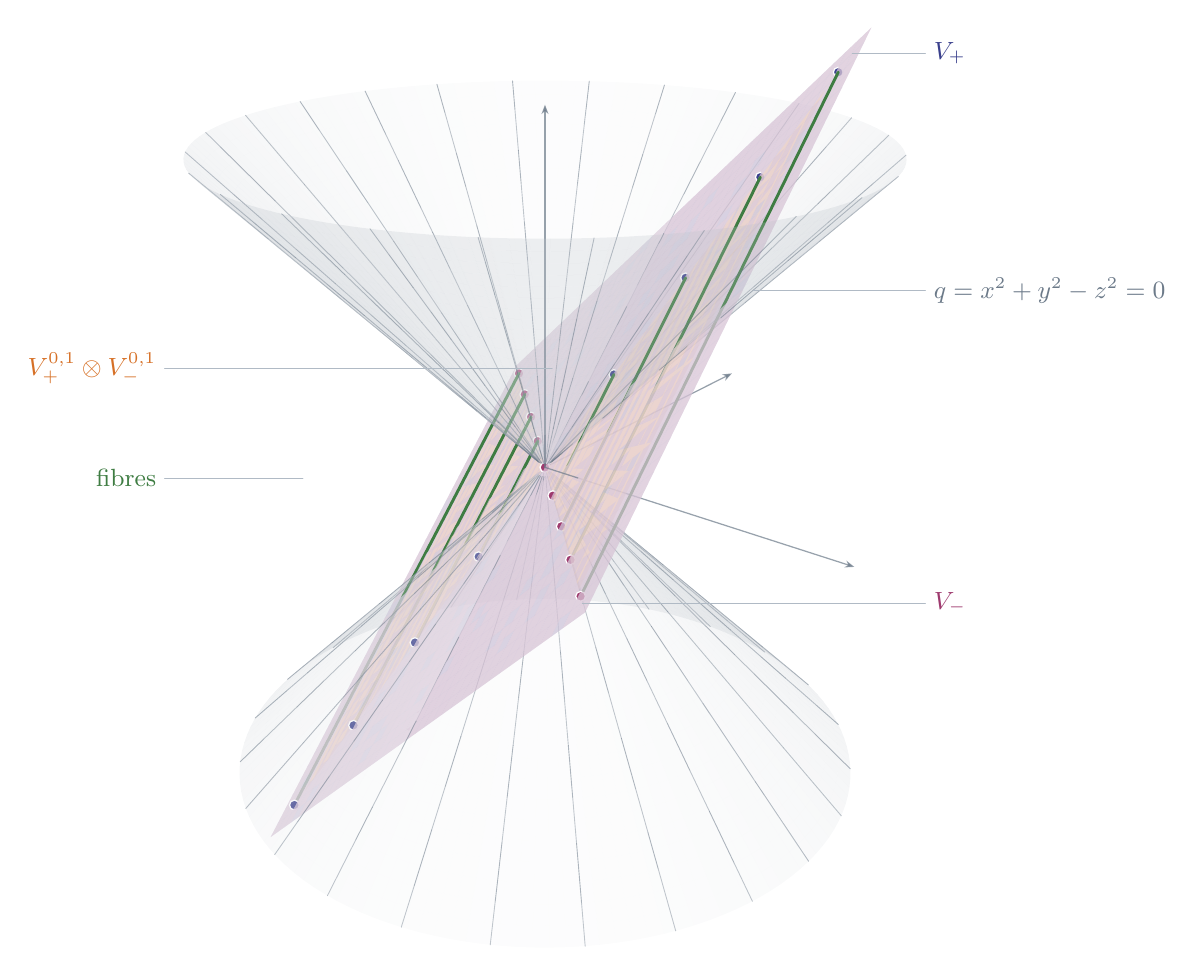
\begin{tikzpicture}[x=1cm,y=1cm,line join=round,line cap=round,
  font=\small,text=PInk]
  \path[draw=none,fill opacity=0.26,fill=PSlate!43!white] (0.0362,-1.7805) -- (-0.1102,-1.7814) -- (-0.1139,-1.8354) -- (0.0374,-1.8346) -- cycle;
  \path[draw=none,fill opacity=0.26,fill=PSlate!43!white] (0.1826,-1.7830) -- (0.0362,-1.7805) -- (0.0374,-1.8346) -- (0.1887,-1.8371) -- cycle;
  \path[draw=none,fill opacity=0.26,fill=PSlate!43!white] (-0.1102,-1.7814) -- (-0.2565,-1.7854) -- (-0.2651,-1.8397) -- (-0.1139,-1.8354) -- cycle;
  \path[draw=none,fill opacity=0.26,fill=PSlate!43!white] (0.3288,-1.7886) -- (0.1826,-1.7830) -- (0.1887,-1.8371) -- (0.3398,-1.8430) -- cycle;
  \path[draw=none,fill opacity=0.26,fill=PSlate!43!white] (-0.2565,-1.7854) -- (-0.4025,-1.7927) -- (-0.4159,-1.8473) -- (-0.2651,-1.8397) -- cycle;
  \path[draw=none,fill opacity=0.26,fill=PSlate!43!white] (0.4745,-1.7975) -- (0.3288,-1.7886) -- (0.3398,-1.8430) -- (0.4904,-1.8523) -- cycle;
  \path[draw=none,fill opacity=0.26,fill=PSlate!44!white] (-0.4025,-1.7927) -- (-0.5479,-1.8033) -- (-0.5663,-1.8582) -- (-0.4159,-1.8473) -- cycle;
  \path[draw=none,fill opacity=0.26,fill=PSlate!43!white] (0.6197,-1.8097) -- (0.4745,-1.7975) -- (0.4904,-1.8523) -- (0.6405,-1.8649) -- cycle;
  \path[draw=none,fill opacity=0.26,fill=PSlate!44!white] (-0.5479,-1.8033) -- (-0.6927,-1.8171) -- (-0.7160,-1.8725) -- (-0.5663,-1.8582) -- cycle;
  \path[draw=none,fill opacity=0.26,fill=PSlate!43!white] (0.7641,-1.8251) -- (0.6197,-1.8097) -- (0.6405,-1.8649) -- (0.7898,-1.8809) -- cycle;
  \path[draw=none,fill opacity=0.26,fill=PSlate!44!white] (-0.6927,-1.8171) -- (-0.8367,-1.8341) -- (-0.8648,-1.8902) -- (-0.7160,-1.8725) -- cycle;
  \path[draw=none,fill opacity=0.26,fill=PSlate!44!white] (0.9075,-1.8437) -- (0.7641,-1.8251) -- (0.7898,-1.8809) -- (0.9381,-1.9002) -- cycle;
  \path[draw=none,fill opacity=0.26,fill=PSlate!44!white] (-0.8367,-1.8341) -- (-0.9795,-1.8543) -- (-1.0126,-1.9113) -- (-0.8648,-1.8902) -- cycle;
  \path[draw=none,fill opacity=0.26,fill=PSlate!44!white] (1.0498,-1.8655) -- (0.9075,-1.8437) -- (0.9381,-1.9002) -- (1.0852,-1.9229) -- cycle;
  \path[draw=none,fill opacity=0.26,fill=PSlate!45!white] (-0.9795,-1.8543) -- (-1.1212,-1.8778) -- (-1.1591,-1.9356) -- (-1.0126,-1.9113) -- cycle;
  \path[draw=none,fill opacity=0.26,fill=PSlate!43!white] (0.0350,-1.7255) -- (-0.1064,-1.7263) -- (-0.1102,-1.7814) -- (0.0362,-1.7805) -- cycle;
  \path[draw=none,fill opacity=0.26,fill=PSlate!43!white] (0.1764,-1.7279) -- (0.0350,-1.7255) -- (0.0362,-1.7805) -- (0.1826,-1.7830) -- cycle;
  \path[draw=none,fill opacity=0.26,fill=PSlate!43!white] (-0.1064,-1.7263) -- (-0.2477,-1.7302) -- (-0.2565,-1.7854) -- (-0.1102,-1.7814) -- cycle;
  \path[draw=none,fill opacity=0.26,fill=PSlate!43!white] (0.3176,-1.7333) -- (0.1764,-1.7279) -- (0.1826,-1.7830) -- (0.3288,-1.7886) -- cycle;
  \path[draw=none,fill opacity=0.26,fill=PSlate!44!white] (1.1908,-1.8906) -- (1.0498,-1.8655) -- (1.0852,-1.9229) -- (1.2311,-1.9490) -- cycle;
  \path[draw=none,fill opacity=0.26,fill=PSlate!43!white] (-0.2477,-1.7302) -- (-0.3887,-1.7372) -- (-0.4025,-1.7927) -- (-0.2565,-1.7854) -- cycle;
  \path[draw=none,fill opacity=0.26,fill=PSlate!43!white] (0.4583,-1.7419) -- (0.3176,-1.7333) -- (0.3288,-1.7886) -- (0.4745,-1.7975) -- cycle;
  \path[draw=none,fill opacity=0.26,fill=PSlate!44!white] (-0.3887,-1.7372) -- (-0.5292,-1.7474) -- (-0.5479,-1.8033) -- (-0.4025,-1.7927) -- cycle;
  \path[draw=none,fill opacity=0.26,fill=PSlate!45!white] (-1.1212,-1.8778) -- (-1.2614,-1.9045) -- (-1.3041,-1.9634) -- (-1.1591,-1.9356) -- cycle;
  \path[draw=none,fill opacity=0.26,fill=PSlate!43!white] (0.5985,-1.7535) -- (0.4583,-1.7419) -- (0.4745,-1.7975) -- (0.6197,-1.8097) -- cycle;
  \path[draw=none,fill opacity=0.26,fill=PSlate!44!white] (-0.5292,-1.7474) -- (-0.6691,-1.7606) -- (-0.6927,-1.8171) -- (-0.5479,-1.8033) -- cycle;
  \path[draw=none,fill opacity=0.26,fill=PSlate!44!white] (1.3302,-1.9188) -- (1.1908,-1.8906) -- (1.2311,-1.9490) -- (1.3753,-1.9783) -- cycle;
  \path[draw=none,fill opacity=0.26,fill=PSlate!43!white] (0.7380,-1.7683) -- (0.5985,-1.7535) -- (0.6197,-1.8097) -- (0.7641,-1.8251) -- cycle;
  \path[draw=none,fill opacity=0.26,fill=PSlate!44!white] (-0.6691,-1.7606) -- (-0.8080,-1.7770) -- (-0.8367,-1.8341) -- (-0.6927,-1.8171) -- cycle;
  \path[draw=none,fill opacity=0.26,fill=PSlate!45!white] (-1.2614,-1.9045) -- (-1.4000,-1.9343) -- (-1.4476,-1.9945) -- (-1.3041,-1.9634) -- cycle;
  \path[draw=none,fill opacity=0.26,fill=PSlate!44!white] (0.8764,-1.7862) -- (0.7380,-1.7683) -- (0.7641,-1.8251) -- (0.9075,-1.8437) -- cycle;
  \path[draw=none,fill opacity=0.26,fill=PSlate!44!white] (-0.8080,-1.7770) -- (-0.9460,-1.7964) -- (-0.9795,-1.8543) -- (-0.8367,-1.8341) -- cycle;
  \path[draw=none,fill opacity=0.26,fill=PSlate!45!white] (1.4679,-1.9503) -- (1.3302,-1.9188) -- (1.3753,-1.9783) -- (1.5179,-2.0111) -- cycle;
  \path[draw=none,fill opacity=0.26,fill=PSlate!44!white] (1.0138,-1.8072) -- (0.8764,-1.7862) -- (0.9075,-1.8437) -- (1.0498,-1.8655) -- cycle;
  \path[draw=none,fill opacity=0.26,fill=PSlate!46!white] (-1.4000,-1.9343) -- (-1.5368,-1.9674) -- (-1.5892,-2.0288) -- (-1.4476,-1.9945) -- cycle;
  \path[draw=none,fill opacity=0.26,fill=PSlate!45!white] (-0.9460,-1.7964) -- (-1.0827,-1.8189) -- (-1.1212,-1.8778) -- (-0.9795,-1.8543) -- cycle;
  \draw[PSlate,line width=0.32pt,opacity=0.55] (-0.3016,-1.5739) -- (-0.3214,-1.6665) -- (-0.3407,-1.7565) -- (-0.3594,-1.8440);
  \path[draw=none,fill opacity=0.26,fill=PSlate!43!white] (0.0337,-1.6695) -- (-0.1026,-1.6703) -- (-0.1064,-1.7263) -- (0.0350,-1.7255) -- cycle;
  \path[draw=none,fill opacity=0.26,fill=PSlate!43!white] (0.1701,-1.6718) -- (0.0337,-1.6695) -- (0.0350,-1.7255) -- (0.1764,-1.7279) -- cycle;
  \path[draw=none,fill opacity=0.26,fill=PSlate!43!white] (-0.1026,-1.6703) -- (-0.2389,-1.6740) -- (-0.2477,-1.7302) -- (-0.1064,-1.7263) -- cycle;
  \path[draw=none,fill opacity=0.26,fill=PSlate!44!white] (1.1498,-1.8312) -- (1.0138,-1.8072) -- (1.0498,-1.8655) -- (1.1908,-1.8906) -- cycle;
  \path[draw=none,fill opacity=0.26,fill=PSlate!43!white] (0.3062,-1.6770) -- (0.1701,-1.6718) -- (0.1764,-1.7279) -- (0.3176,-1.7333) -- cycle;
  \path[draw=none,fill opacity=0.26,fill=PSlate!45!white] (1.6038,-1.9850) -- (1.4679,-1.9503) -- (1.5179,-2.0111) -- (1.6585,-2.0471) -- cycle;
  \draw[PSlate,line width=0.32pt,opacity=0.55] (0.4115,-1.5806) -- (0.4385,-1.6737) -- (0.4648,-1.7642) -- (0.4904,-1.8523);
  \path[draw=none,fill opacity=0.26,fill=PSlate!43!white] (-0.2389,-1.6740) -- (-0.3748,-1.6808) -- (-0.3887,-1.7372) -- (-0.2477,-1.7302) -- cycle;
  \path[draw=none,fill opacity=0.26,fill=PSlate!43!white] (0.4419,-1.6852) -- (0.3062,-1.6770) -- (0.3176,-1.7333) -- (0.4583,-1.7419) -- cycle;
  \path[draw=none,fill opacity=0.26,fill=PSlate!45!white] (-1.0827,-1.8189) -- (-1.2180,-1.8446) -- (-1.2614,-1.9045) -- (-1.1212,-1.8778) -- cycle;
  \path[draw=none,fill opacity=0.26,fill=PSlate!44!white] (-0.3748,-1.6808) -- (-0.5102,-1.6905) -- (-0.5292,-1.7474) -- (-0.3887,-1.7372) -- cycle;
  \path[draw=none,fill opacity=0.26,fill=PSlate!43!white] (0.5770,-1.6964) -- (0.4419,-1.6852) -- (0.4583,-1.7419) -- (0.5985,-1.7535) -- cycle;
  \path[draw=none,fill opacity=0.26,fill=PSlate!46!white] (-1.5368,-1.9674) -- (-1.6716,-2.0037) -- (-1.7288,-2.0665) -- (-1.5892,-2.0288) -- cycle;
  \path[draw=none,fill opacity=0.26,fill=PSlate!44!white] (-0.5102,-1.6905) -- (-0.6450,-1.7032) -- (-0.6691,-1.7606) -- (-0.5292,-1.7474) -- cycle;
  \path[draw=none,fill opacity=0.26,fill=PSlate!44!white] (1.2843,-1.8584) -- (1.1498,-1.8312) -- (1.1908,-1.8906) -- (1.3302,-1.9188) -- cycle;
  \path[draw=none,fill opacity=0.26,fill=PSlate!43!white] (0.7114,-1.7106) -- (0.5770,-1.6964) -- (0.5985,-1.7535) -- (0.7380,-1.7683) -- cycle;
  \path[draw=none,fill opacity=0.26,fill=PSlate!46!white] (1.7375,-2.0228) -- (1.6038,-1.9850) -- (1.6585,-2.0471) -- (1.7970,-2.0864) -- cycle;
  \path[draw=none,fill opacity=0.26,fill=PSlate!44!white] (-0.6450,-1.7032) -- (-0.7789,-1.7188) -- (-0.8080,-1.7770) -- (-0.6691,-1.7606) -- cycle;
  \path[draw=none,fill opacity=0.26,fill=PSlate!45!white] (-1.2180,-1.8446) -- (-1.3517,-1.8732) -- (-1.4000,-1.9343) -- (-1.2614,-1.9045) -- cycle;
  \path[draw=none,fill opacity=0.26,fill=PSlate!44!white] (0.8448,-1.7277) -- (0.7114,-1.7106) -- (0.7380,-1.7683) -- (0.8764,-1.7862) -- cycle;
  \path[draw=none,fill opacity=0.26,fill=PSlate!45!white] (1.4172,-1.8886) -- (1.2843,-1.8584) -- (1.3302,-1.9188) -- (1.4679,-1.9503) -- cycle;
  \path[draw=none,fill opacity=0.26,fill=PSlate!44!white] (-0.7789,-1.7188) -- (-0.9118,-1.7375) -- (-0.9460,-1.7964) -- (-0.8080,-1.7770) -- cycle;
  \path[draw=none,fill opacity=0.26,fill=PSlate!46!white] (-1.6716,-2.0037) -- (-1.8041,-2.0431) -- (-1.8661,-2.1076) -- (-1.7288,-2.0665) -- cycle;
  \path[draw=none,fill opacity=0.26,fill=PSlate!44!white] (0.9771,-1.7478) -- (0.8448,-1.7277) -- (0.8764,-1.7862) -- (1.0138,-1.8072) -- cycle;
  \path[draw=none,fill opacity=0.26,fill=PSlate!46!white] (-1.3517,-1.8732) -- (-1.4836,-1.9050) -- (-1.5368,-1.9674) -- (-1.4000,-1.9343) -- cycle;
  \path[draw=none,fill opacity=0.26,fill=PSlate!45!white] (-0.9118,-1.7375) -- (-1.0435,-1.7591) -- (-1.0827,-1.8189) -- (-0.9460,-1.7964) -- cycle;
  \path[draw=none,fill opacity=0.26,fill=PSlate!46!white] (1.8689,-2.0637) -- (1.7375,-2.0228) -- (1.7970,-2.0864) -- (1.9332,-2.1291) -- cycle;
  \draw[PSlate,line width=0.32pt,opacity=0.55] (-1.0017,-1.6541) -- (-1.0680,-1.7528) -- (-1.1326,-1.8488) -- (-1.1955,-1.9423);
  \path[draw=none,fill opacity=0.26,fill=PSlate!45!white] (1.5481,-1.9218) -- (1.4172,-1.8886) -- (1.4679,-1.9503) -- (1.6038,-1.9850) -- cycle;
  \path[draw=none,fill opacity=0.26,fill=PSlate!44!white] (1.1082,-1.7709) -- (0.9771,-1.7478) -- (1.0138,-1.8072) -- (1.1498,-1.8312) -- cycle;
  \path[draw=none,fill opacity=0.26,fill=PSlate!43!white] (0.0325,-1.6125) -- (-0.0987,-1.6133) -- (-0.1026,-1.6703) -- (0.0337,-1.6695) -- cycle;
  \path[draw=none,fill opacity=0.26,fill=PSlate!43!white] (0.1636,-1.6147) -- (0.0325,-1.6125) -- (0.0337,-1.6695) -- (0.1701,-1.6718) -- cycle;
  \path[draw=none,fill opacity=0.26,fill=PSlate!43!white] (-0.0987,-1.6133) -- (-0.2298,-1.6168) -- (-0.2389,-1.6740) -- (-0.1026,-1.6703) -- cycle;
  \path[draw=none,fill opacity=0.26,fill=PSlate!43!white] (0.2946,-1.6197) -- (0.1636,-1.6147) -- (0.1701,-1.6718) -- (0.3062,-1.6770) -- cycle;
  \path[draw=none,fill opacity=0.26,fill=PSlate!43!white] (-0.2298,-1.6168) -- (-0.3606,-1.6233) -- (-0.3748,-1.6808) -- (-0.2389,-1.6740) -- cycle;
  \path[draw=none,fill opacity=0.26,fill=PSlate!46!white] (-1.8041,-2.0431) -- (-1.9343,-2.0856) -- (-2.0010,-2.1518) -- (-1.8661,-2.1076) -- cycle;
  \path[draw=none,fill opacity=0.26,fill=PSlate!43!white] (0.4251,-1.6275) -- (0.2946,-1.6197) -- (0.3062,-1.6770) -- (0.4419,-1.6852) -- cycle;
  \path[draw=none,fill opacity=0.26,fill=PSlate!45!white] (-1.0435,-1.7591) -- (-1.1738,-1.7836) -- (-1.2180,-1.8446) -- (-1.0827,-1.8189) -- cycle;
  \path[draw=none,fill opacity=0.26,fill=PSlate!46!white] (-1.4836,-1.9050) -- (-1.6135,-1.9398) -- (-1.6716,-2.0037) -- (-1.5368,-1.9674) -- cycle;
  \path[draw=none,fill opacity=0.26,fill=PSlate!44!white] (-0.3606,-1.6233) -- (-0.4908,-1.6326) -- (-0.5102,-1.6905) -- (-0.3748,-1.6808) -- cycle;
  \draw[PSlate,line width=0.32pt,opacity=0.55] (1.1068,-1.6742) -- (1.1803,-1.7744) -- (1.2518,-1.8720) -- (1.3214,-1.9669);
  \path[draw=none,fill opacity=0.26,fill=PSlate!43!white] (0.5551,-1.6382) -- (0.4251,-1.6275) -- (0.4419,-1.6852) -- (0.5770,-1.6964) -- cycle;
  \path[draw=none,fill opacity=0.26,fill=PSlate!44!white] (1.2377,-1.7969) -- (1.1082,-1.7709) -- (1.1498,-1.8312) -- (1.2843,-1.8584) -- cycle;
  \path[draw=none,fill opacity=0.26,fill=PSlate!44!white] (-0.4908,-1.6326) -- (-0.6205,-1.6447) -- (-0.6450,-1.7032) -- (-0.5102,-1.6905) -- cycle;
  \path[draw=none,fill opacity=0.26,fill=PSlate!46!white] (1.9977,-2.1078) -- (1.8689,-2.0637) -- (1.9332,-2.1291) -- (2.0667,-2.1750) -- cycle;
  \path[draw=none,fill opacity=0.26,fill=PSlate!46!white] (1.6770,-1.9581) -- (1.5481,-1.9218) -- (1.6038,-1.9850) -- (1.7375,-2.0228) -- cycle;
  \path[draw=none,fill opacity=0.26,fill=PSlate!43!white] (0.6843,-1.6518) -- (0.5551,-1.6382) -- (0.5770,-1.6964) -- (0.7114,-1.7106) -- cycle;
  \path[draw=none,fill opacity=0.26,fill=PSlate!45!white] (-1.1738,-1.7836) -- (-1.3025,-1.8111) -- (-1.3517,-1.8732) -- (-1.2180,-1.8446) -- cycle;
  \path[draw=none,fill opacity=0.26,fill=PSlate!44!white] (-0.6205,-1.6447) -- (-0.7493,-1.6597) -- (-0.7789,-1.7188) -- (-0.6450,-1.7032) -- cycle;
  \path[draw=none,fill opacity=0.26,fill=PSlate!44!white] (0.8126,-1.6682) -- (0.6843,-1.6518) -- (0.7114,-1.7106) -- (0.8448,-1.7277) -- cycle;
  \path[draw=none,fill opacity=0.26,fill=PSlate!46!white] (-1.6135,-1.9398) -- (-1.7412,-1.9776) -- (-1.8041,-2.0431) -- (-1.6716,-2.0037) -- cycle;
  \path[draw=none,fill opacity=0.26,fill=PSlate!45!white] (1.3656,-1.8258) -- (1.2377,-1.7969) -- (1.2843,-1.8584) -- (1.4172,-1.8886) -- cycle;
  \path[draw=none,fill opacity=0.26,fill=PSlate!46!white] (-1.9343,-2.0856) -- (-2.0618,-2.1313) -- (-2.1332,-2.1994) -- (-2.0010,-2.1518) -- cycle;
  \path[draw=none,fill opacity=0.26,fill=PSlate!44!white] (-0.7493,-1.6597) -- (-0.8770,-1.6775) -- (-0.9118,-1.7375) -- (-0.7789,-1.7188) -- cycle;
  \path[draw=none,fill opacity=0.26,fill=PSlate!44!white] (0.9398,-1.6874) -- (0.8126,-1.6682) -- (0.8448,-1.7277) -- (0.9771,-1.7478) -- cycle;
  \path[draw=none,fill opacity=0.26,fill=PSlate!46!white] (-1.3025,-1.8111) -- (-1.4295,-1.8415) -- (-1.4836,-1.9050) -- (-1.3517,-1.8732) -- cycle;
  \path[draw=none,fill opacity=0.26,fill=PSlate!46!white] (1.8036,-1.9974) -- (1.6770,-1.9581) -- (1.7375,-2.0228) -- (1.8689,-2.0637) -- cycle;
  \path[draw=none,fill opacity=0.26,fill=PSlate!46!white] (2.1239,-2.1550) -- (1.9977,-2.1078) -- (2.0667,-2.1750) -- (2.1976,-2.2241) -- cycle;
  \path[draw=none,fill opacity=0.26,fill=PSlate!45!white] (-0.8770,-1.6775) -- (-1.0036,-1.6982) -- (-1.0435,-1.7591) -- (-0.9118,-1.7375) -- cycle;
  \path[draw=none,fill opacity=0.26,fill=PSlate!45!white] (1.4916,-1.8576) -- (1.3656,-1.8258) -- (1.4172,-1.8886) -- (1.5481,-1.9218) -- cycle;
  \path[draw=none,fill opacity=0.26,fill=PSlate!44!white] (1.0658,-1.7095) -- (0.9398,-1.6874) -- (0.9771,-1.7478) -- (1.1082,-1.7709) -- cycle;
  \path[draw=none,fill opacity=0.26,fill=PSlate!46!white] (-1.7412,-1.9776) -- (-1.8666,-2.0184) -- (-1.9343,-2.0856) -- (-1.8041,-2.0431) -- cycle;
  \path[draw=none,fill opacity=0.26,fill=PSlate!43!white] (0.0312,-1.5545) -- (-0.0948,-1.5552) -- (-0.0987,-1.6133) -- (0.0325,-1.6125) -- cycle;
  \path[draw=none,fill opacity=0.26,fill=PSlate!43!white] (0.1571,-1.5566) -- (0.0312,-1.5545) -- (0.0325,-1.6125) -- (0.1636,-1.6147) -- cycle;
  \path[draw=none,fill opacity=0.26,fill=PSlate!43!white] (-0.0948,-1.5552) -- (-0.2206,-1.5586) -- (-0.2298,-1.6168) -- (-0.0987,-1.6133) -- cycle;
  \path[draw=none,fill opacity=0.26,fill=PSlate!43!white] (0.2827,-1.5613) -- (0.1571,-1.5566) -- (0.1636,-1.6147) -- (0.2946,-1.6197) -- cycle;
  \path[draw=none,fill opacity=0.26,fill=PSlate!46!white] (-2.0618,-2.1313) -- (-2.1865,-2.1801) -- (-2.2625,-2.2502) -- (-2.1332,-2.1994) -- cycle;
  \path[draw=none,fill opacity=0.26,fill=PSlate!46!white] (-1.4295,-1.8415) -- (-1.5544,-1.8748) -- (-1.6135,-1.9398) -- (-1.4836,-1.9050) -- cycle;
  \path[draw=none,fill opacity=0.26,fill=PSlate!45!white] (-1.0036,-1.6982) -- (-1.1289,-1.7217) -- (-1.1738,-1.7836) -- (-1.0435,-1.7591) -- cycle;
  \path[draw=none,fill opacity=0.26,fill=PSlate!43!white] (-0.2206,-1.5586) -- (-0.3461,-1.5648) -- (-0.3606,-1.6233) -- (-0.2298,-1.6168) -- cycle;
  \path[draw=none,fill opacity=0.26,fill=PSlate!43!white] (0.4080,-1.5688) -- (0.2827,-1.5613) -- (0.2946,-1.6197) -- (0.4251,-1.6275) -- cycle;
  \path[draw=none,fill opacity=0.26,fill=PSlate!44!white] (-0.3461,-1.5648) -- (-0.4711,-1.5736) -- (-0.4908,-1.6326) -- (-0.3606,-1.6233) -- cycle;
  \path[draw=none,fill opacity=0.26,fill=PSlate!46!white] (1.9276,-2.0397) -- (1.8036,-1.9974) -- (1.8689,-2.0637) -- (1.9977,-2.1078) -- cycle;
  \path[draw=none,fill opacity=0.26,fill=PSlate!44!white] (1.1903,-1.7343) -- (1.0658,-1.7095) -- (1.1082,-1.7709) -- (1.2377,-1.7969) -- cycle;
  \path[draw=none,fill opacity=0.26,fill=PSlate!43!white] (0.5328,-1.5790) -- (0.4080,-1.5688) -- (0.4251,-1.6275) -- (0.5551,-1.6382) -- cycle;
  \path[draw=none,fill opacity=0.26,fill=PSlate!46!white] (1.6155,-1.8924) -- (1.4916,-1.8576) -- (1.5481,-1.9218) -- (1.6770,-1.9581) -- cycle;
  \path[draw=none,fill opacity=0.26,fill=PSlate!44!white] (-0.4711,-1.5736) -- (-0.5955,-1.5852) -- (-0.6205,-1.6447) -- (-0.4908,-1.6326) -- cycle;
  \path[draw=none,fill opacity=0.26,fill=PSlate!46!white] (2.2470,-2.2053) -- (2.1239,-2.1550) -- (2.1976,-2.2241) -- (2.3254,-2.2765) -- cycle;
  \path[draw=none,fill opacity=0.26,fill=PSlate!43!white] (0.6568,-1.5920) -- (0.5328,-1.5790) -- (0.5551,-1.6382) -- (0.6843,-1.6518) -- cycle;
  \path[draw=none,fill opacity=0.26,fill=PSlate!45!white] (-1.1289,-1.7217) -- (-1.2525,-1.7479) -- (-1.3025,-1.8111) -- (-1.1738,-1.7836) -- cycle;
  \path[draw=none,fill opacity=0.26,fill=PSlate!44!white] (-0.5955,-1.5852) -- (-0.7191,-1.5995) -- (-0.7493,-1.6597) -- (-0.6205,-1.6447) -- cycle;
  \path[draw=none,fill opacity=0.26,fill=PSlate!46!white] (-1.8666,-2.0184) -- (-1.9893,-2.0622) -- (-2.0618,-2.1313) -- (-1.9343,-2.0856) -- cycle;
  \path[draw=none,fill opacity=0.26,fill=PSlate!46!white] (-1.5544,-1.8748) -- (-1.6773,-1.9110) -- (-1.7412,-1.9776) -- (-1.6135,-1.9398) -- cycle;
  \path[draw=none,fill opacity=0.26,fill=PSlate!45!white] (1.3131,-1.7620) -- (1.1903,-1.7343) -- (1.2377,-1.7969) -- (1.3656,-1.8258) -- cycle;
  \path[draw=none,fill opacity=0.26,fill=PSlate!44!white] (0.7799,-1.6076) -- (0.6568,-1.5920) -- (0.6843,-1.6518) -- (0.8126,-1.6682) -- cycle;
  \path[draw=none,fill opacity=0.26,fill=PSlate!46!white] (-2.1865,-2.1801) -- (-2.3081,-2.2319) -- (-2.3887,-2.3042) -- (-2.2625,-2.2502) -- cycle;
  \path[draw=none,fill opacity=0.26,fill=PSlate!44!white] (-0.7191,-1.5995) -- (-0.8417,-1.6165) -- (-0.8770,-1.6775) -- (-0.7493,-1.6597) -- cycle;
  \path[draw=none,fill opacity=0.26,fill=PSlate!46!white] (1.7372,-1.9300) -- (1.6155,-1.8924) -- (1.6770,-1.9581) -- (1.8036,-1.9974) -- cycle;
  \path[draw=none,fill opacity=0.26,fill=PSlate!46!white] (-1.2525,-1.7479) -- (-1.3744,-1.7770) -- (-1.4295,-1.8415) -- (-1.3025,-1.8111) -- cycle;
  \path[draw=none,fill opacity=0.26,fill=PSlate!46!white] (2.0490,-2.0849) -- (1.9276,-2.0397) -- (1.9977,-2.1078) -- (2.1239,-2.1550) -- cycle;
  \path[draw=none,fill opacity=0.26,fill=PSlate!44!white] (0.9019,-1.6260) -- (0.7799,-1.6076) -- (0.8126,-1.6682) -- (0.9398,-1.6874) -- cycle;
  \path[draw=none,fill opacity=0.26,fill=PSlate!45!white] (-0.8417,-1.6165) -- (-0.9631,-1.6362) -- (-1.0036,-1.6982) -- (-0.8770,-1.6775) -- cycle;
  \path[draw=none,fill opacity=0.26,fill=PSlate!45!white] (1.4341,-1.7924) -- (1.3131,-1.7620) -- (1.3656,-1.8258) -- (1.4916,-1.8576) -- cycle;
  \path[draw=none,fill opacity=0.26,fill=PSlate!46!white] (-1.6773,-1.9110) -- (-1.7978,-1.9501) -- (-1.8666,-2.0184) -- (-1.7412,-1.9776) -- cycle;
  \path[draw=none,fill opacity=0.26,fill=PSlate!46!white] (2.3670,-2.2587) -- (2.2470,-2.2053) -- (2.3254,-2.2765) -- (2.4500,-2.3320) -- cycle;
  \path[draw=none,fill opacity=0.26,fill=PSlate!46!white] (-1.9893,-2.0622) -- (-2.1093,-2.1089) -- (-2.1865,-2.1801) -- (-2.0618,-2.1313) -- cycle;
  \path[draw=none,fill opacity=0.26,fill=PSlate!44!white] (1.0227,-1.6470) -- (0.9019,-1.6260) -- (0.9398,-1.6874) -- (1.0658,-1.7095) -- cycle;
  \draw[PSlate,line width=0.32pt,opacity=0.55] (-1.6574,-1.8197) -- (-1.7691,-1.9313) -- (-1.8780,-2.0400) -- (-1.9842,-2.1461);
  \path[draw=none,fill opacity=0.26,fill=PSlate!46!white] (-1.3744,-1.7770) -- (-1.4944,-1.8088) -- (-1.5544,-1.8748) -- (-1.4295,-1.8415) -- cycle;
  \path[draw=none,fill opacity=0.26,fill=PSlate!43!white] (0.0298,-1.4954) -- (-0.0907,-1.4961) -- (-0.0948,-1.5552) -- (0.0312,-1.5545) -- cycle;
  \path[draw=none,fill opacity=0.26,fill=PSlate!43!white] (0.1504,-1.4974) -- (0.0298,-1.4954) -- (0.0312,-1.5545) -- (0.1571,-1.5566) -- cycle;
  \path[draw=none,fill opacity=0.26,fill=PSlate!45!white] (-0.9631,-1.6362) -- (-1.0831,-1.6586) -- (-1.1289,-1.7217) -- (-1.0036,-1.6982) -- cycle;
  \path[draw=none,fill opacity=0.26,fill=PSlate!43!white] (-0.0907,-1.4961) -- (-0.2112,-1.4993) -- (-0.2206,-1.5586) -- (-0.0948,-1.5552) -- cycle;
  \path[draw=none,fill opacity=0.26,fill=PSlate!43!white] (0.2707,-1.5019) -- (0.1504,-1.4974) -- (0.1571,-1.5566) -- (0.2827,-1.5613) -- cycle;
  \path[draw=none,fill opacity=0.26,fill=PSlate!46!white] (1.8565,-1.9704) -- (1.7372,-1.9300) -- (1.8036,-1.9974) -- (1.9276,-2.0397) -- cycle;
  \path[draw=none,fill opacity=0.26,fill=PSlate!43!white] (-0.2112,-1.4993) -- (-0.3314,-1.5052) -- (-0.3461,-1.5648) -- (-0.2206,-1.5586) -- cycle;
  \path[draw=none,fill opacity=0.26,fill=PSlate!43!white] (0.3907,-1.5090) -- (0.2707,-1.5019) -- (0.2827,-1.5613) -- (0.4080,-1.5688) -- cycle;
  \path[draw=none,fill opacity=0.26,fill=PSlate!46!white] (-2.3081,-2.2319) -- (-2.4264,-2.2868) -- (-2.5116,-2.3613) -- (-2.3887,-2.3042) -- cycle;
  \path[draw=none,fill opacity=0.26,fill=PSlate!46!white] (2.1675,-2.1331) -- (2.0490,-2.0849) -- (2.1239,-2.1550) -- (2.2470,-2.2053) -- cycle;
  \path[draw=none,fill opacity=0.26,fill=PSlate!46!white] (1.5530,-1.8256) -- (1.4341,-1.7924) -- (1.4916,-1.8576) -- (1.6155,-1.8924) -- cycle;
  \path[draw=none,fill opacity=0.26,fill=PSlate!44!white] (1.1420,-1.6707) -- (1.0227,-1.6470) -- (1.0658,-1.7095) -- (1.1903,-1.7343) -- cycle;
  \path[draw=none,fill opacity=0.26,fill=PSlate!44!white] (-0.3314,-1.5052) -- (-0.4511,-1.5136) -- (-0.4711,-1.5736) -- (-0.3461,-1.5648) -- cycle;
  \path[draw=none,fill opacity=0.26,fill=PSlate!43!white] (0.5101,-1.5188) -- (0.3907,-1.5090) -- (0.4080,-1.5688) -- (0.5328,-1.5790) -- cycle;
  \path[draw=none,fill opacity=0.26,fill=PSlate!44!white] (-0.4511,-1.5136) -- (-0.5701,-1.5247) -- (-0.5955,-1.5852) -- (-0.4711,-1.5736) -- cycle;
  \path[draw=none,fill opacity=0.26,fill=PSlate!46!white] (-1.7978,-1.9501) -- (-1.9157,-1.9920) -- (-1.9893,-2.0622) -- (-1.8666,-2.0184) -- cycle;
  \path[draw=none,fill opacity=0.26,fill=PSlate!45!white] (-1.0831,-1.6586) -- (-1.2017,-1.6837) -- (-1.2525,-1.7479) -- (-1.1289,-1.7217) -- cycle;
  \draw[PSlate,line width=0.32pt,opacity=0.55] (1.7527,-1.8528) -- (1.8713,-1.9669) -- (1.9869,-2.0783) -- (2.0997,-2.1869);
  \path[draw=none,fill opacity=0.26,fill=PSlate!43!white] (0.6288,-1.5311) -- (0.5101,-1.5188) -- (0.5328,-1.5790) -- (0.6568,-1.5920) -- cycle;
  \path[draw=none,fill opacity=0.26,fill=PSlate!46!white] (-1.4944,-1.8088) -- (-1.6123,-1.8434) -- (-1.6773,-1.9110) -- (-1.5544,-1.8748) -- cycle;
  \path[draw=none,fill opacity=0.26,fill=PSlate!46!white] (-2.1093,-2.1089) -- (-2.2262,-2.1586) -- (-2.3081,-2.2319) -- (-2.1865,-2.1801) -- cycle;
  \path[draw=none,fill opacity=0.26,fill=PSlate!44!white] (-0.5701,-1.5247) -- (-0.6884,-1.5383) -- (-0.7191,-1.5995) -- (-0.5955,-1.5852) -- cycle;
  \path[draw=none,fill opacity=0.26,fill=PSlate!46!white] (2.4836,-2.3150) -- (2.3670,-2.2587) -- (2.4500,-2.3320) -- (2.5711,-2.3908) -- cycle;
  \path[draw=none,fill opacity=0.26,fill=PSlate!45!white] (1.2597,-1.6970) -- (1.1420,-1.6707) -- (1.1903,-1.7343) -- (1.3131,-1.7620) -- cycle;
  \path[draw=none,fill opacity=0.26,fill=PSlate!44!white] (0.7466,-1.5460) -- (0.6288,-1.5311) -- (0.6568,-1.5920) -- (0.7799,-1.6076) -- cycle;
  \path[draw=none,fill opacity=0.26,fill=PSlate!46!white] (1.9731,-2.0137) -- (1.8565,-1.9704) -- (1.9276,-2.0397) -- (2.0490,-2.0849) -- cycle;
  \path[draw=none,fill opacity=0.26,fill=PSlate!46!white] (1.6698,-1.8615) -- (1.5530,-1.8256) -- (1.6155,-1.8924) -- (1.7372,-1.9300) -- cycle;
  \path[draw=none,fill opacity=0.26,fill=PSlate!44!white] (-0.6884,-1.5383) -- (-0.8057,-1.5545) -- (-0.8417,-1.6165) -- (-0.7191,-1.5995) -- cycle;
  \path[draw=none,fill opacity=0.26,fill=PSlate!46!white] (-1.2017,-1.6837) -- (-1.3185,-1.7114) -- (-1.3744,-1.7770) -- (-1.2525,-1.7479) -- cycle;
  \path[draw=none,fill opacity=0.26,fill=PSlate!44!white] (0.8633,-1.5634) -- (0.7466,-1.5460) -- (0.7799,-1.6076) -- (0.9019,-1.6260) -- cycle;
  \path[draw=none,fill opacity=0.26,fill=PSlate!46!white] (2.2829,-2.1842) -- (2.1675,-2.1331) -- (2.2470,-2.2053) -- (2.3670,-2.2587) -- cycle;
  \path[draw=none,fill opacity=0.26,fill=PSlate!46!white] (-2.4264,-2.2868) -- (-2.5412,-2.3446) -- (-2.6310,-2.4216) -- (-2.5116,-2.3613) -- cycle;
  \path[draw=none,fill opacity=0.26,fill=PSlate!46!white] (-1.6123,-1.8434) -- (-1.7279,-1.8807) -- (-1.7978,-1.9501) -- (-1.6773,-1.9110) -- cycle;
  \path[draw=none,fill opacity=0.26,fill=PSlate!45!white] (1.3756,-1.7261) -- (1.2597,-1.6970) -- (1.3131,-1.7620) -- (1.4341,-1.7924) -- cycle;
  \path[draw=none,fill opacity=0.26,fill=PSlate!46!white] (-1.9157,-1.9920) -- (-2.0309,-2.0367) -- (-2.1093,-2.1089) -- (-1.9893,-2.0622) -- cycle;
  \path[draw=none,fill opacity=0.26,fill=PSlate!45!white] (-0.8057,-1.5545) -- (-0.9218,-1.5732) -- (-0.9631,-1.6362) -- (-0.8417,-1.6165) -- cycle;
  \path[draw=none,fill opacity=0.26,fill=PSlate!44!white] (0.9788,-1.5834) -- (0.8633,-1.5634) -- (0.9019,-1.6260) -- (1.0227,-1.6470) -- cycle;
  \path[draw=none,fill opacity=0.26,fill=PSlate!46!white] (-1.3185,-1.7114) -- (-1.4334,-1.7417) -- (-1.4944,-1.8088) -- (-1.3744,-1.7770) -- cycle;
  \path[draw=none,fill opacity=0.26,fill=PSlate!46!white] (1.7842,-1.9001) -- (1.6698,-1.8615) -- (1.7372,-1.9300) -- (1.8565,-1.9704) -- cycle;
  \path[draw=none,fill opacity=0.26,fill=PSlate!46!white] (-2.2262,-2.1586) -- (-2.3399,-2.2111) -- (-2.4264,-2.2868) -- (-2.3081,-2.2319) -- cycle;
  \path[draw=none,fill opacity=0.26,fill=PSlate!46!white] (2.0868,-2.0598) -- (1.9731,-2.0137) -- (2.0490,-2.0849) -- (2.1675,-2.1331) -- cycle;
  \path[draw=none,fill opacity=0.26,fill=PSlate!45!white] (-0.9218,-1.5732) -- (-1.0366,-1.5945) -- (-1.0831,-1.6586) -- (-0.9631,-1.6362) -- cycle;
  \path[draw=none,fill opacity=0.26,fill=PSlate!43!white] (0.0285,-1.4353) -- (-0.0866,-1.4359) -- (-0.0907,-1.4961) -- (0.0298,-1.4954) -- cycle;
  \path[draw=none,fill opacity=0.26,fill=PSlate!46!white] (2.5966,-2.3744) -- (2.4836,-2.3150) -- (2.5711,-2.3908) -- (2.6886,-2.4527) -- cycle;
  \path[draw=none,fill opacity=0.26,fill=PSlate!43!white] (0.1436,-1.4371) -- (0.0285,-1.4353) -- (0.0298,-1.4954) -- (0.1504,-1.4974) -- cycle;
  \path[draw=none,fill opacity=0.26,fill=PSlate!43!white] (-0.0866,-1.4359) -- (-0.2016,-1.4390) -- (-0.2112,-1.4993) -- (-0.0907,-1.4961) -- cycle;
  \path[draw=none,fill opacity=0.26,fill=PSlate!43!white] (0.2585,-1.4414) -- (0.1436,-1.4371) -- (0.1504,-1.4974) -- (0.2707,-1.5019) -- cycle;
  \path[draw=none,fill opacity=0.26,fill=PSlate!46!white] (1.4896,-1.7577) -- (1.3756,-1.7261) -- (1.4341,-1.7924) -- (1.5530,-1.8256) -- cycle;
  \path[draw=none,fill opacity=0.26,fill=PSlate!43!white] (-0.2016,-1.4390) -- (-0.3164,-1.4445) -- (-0.3314,-1.5052) -- (-0.2112,-1.4993) -- cycle;
  \path[draw=none,fill opacity=0.26,fill=PSlate!44!white] (1.0929,-1.6060) -- (0.9788,-1.5834) -- (1.0227,-1.6470) -- (1.1420,-1.6707) -- cycle;
  \path[draw=none,fill opacity=0.26,fill=PSlate!43!white] (0.3730,-1.4482) -- (0.2585,-1.4414) -- (0.2707,-1.5019) -- (0.3907,-1.5090) -- cycle;
  \path[draw=none,fill opacity=0.26,fill=PSlate!46!white] (-1.7279,-1.8807) -- (-1.8410,-1.9207) -- (-1.9157,-1.9920) -- (-1.7978,-1.9501) -- cycle;
  \path[draw=none,fill opacity=0.26,fill=PSlate!44!white] (-0.3164,-1.4445) -- (-0.4306,-1.4525) -- (-0.4511,-1.5136) -- (-0.3314,-1.5052) -- cycle;
  \path[draw=none,fill opacity=0.26,fill=PSlate!46!white] (2.3949,-2.2382) -- (2.2829,-2.1842) -- (2.3670,-2.2587) -- (2.4836,-2.3150) -- cycle;
  \path[draw=none,fill opacity=0.26,fill=PSlate!43!white] (0.4870,-1.4574) -- (0.3730,-1.4482) -- (0.3907,-1.5090) -- (0.5101,-1.5188) -- cycle;
  \path[draw=none,fill opacity=0.26,fill=PSlate!46!white] (-2.0309,-2.0367) -- (-2.1431,-2.0842) -- (-2.2262,-2.1586) -- (-2.1093,-2.1089) -- cycle;
  \path[draw=none,fill opacity=0.26,fill=PSlate!45!white] (-1.0366,-1.5945) -- (-1.1500,-1.6183) -- (-1.2017,-1.6837) -- (-1.0831,-1.6586) -- cycle;
  \path[draw=none,fill opacity=0.26,fill=PSlate!46!white] (-1.4334,-1.7417) -- (-1.5463,-1.7746) -- (-1.6123,-1.8434) -- (-1.4944,-1.8088) -- cycle;
  \path[draw=none,fill opacity=0.26,fill=PSlate!44!white] (-0.4306,-1.4525) -- (-0.5443,-1.4630) -- (-0.5701,-1.5247) -- (-0.4511,-1.5136) -- cycle;
  \path[draw=none,fill opacity=0.26,fill=PSlate!43!white] (0.6002,-1.4691) -- (0.4870,-1.4574) -- (0.5101,-1.5188) -- (0.6288,-1.5311) -- cycle;
  \path[draw=none,fill opacity=0.26,fill=PSlate!46!white] (-2.5412,-2.3446) -- (-2.6522,-2.4055) -- (-2.7465,-2.4851) -- (-2.6310,-2.4216) -- cycle;
  \path[draw=none,fill opacity=0.26,fill=PSlate!46!white] (1.8959,-1.9415) -- (1.7842,-1.9001) -- (1.8565,-1.9704) -- (1.9731,-2.0137) -- cycle;
  \path[draw=none,fill opacity=0.26,fill=PSlate!45!white] (1.2054,-1.6310) -- (1.0929,-1.6060) -- (1.1420,-1.6707) -- (1.2597,-1.6970) -- cycle;
  \path[draw=none,fill opacity=0.26,fill=PSlate!44!white] (-0.5443,-1.4630) -- (-0.6571,-1.4759) -- (-0.6884,-1.5383) -- (-0.5701,-1.5247) -- cycle;
  \path[draw=none,fill opacity=0.26,fill=PSlate!46!white] (1.6013,-1.7919) -- (1.4896,-1.7577) -- (1.5530,-1.8256) -- (1.6698,-1.8615) -- cycle;
  \path[draw=none,fill opacity=0.26,fill=PSlate!44!white] (0.7126,-1.4832) -- (0.6002,-1.4691) -- (0.6288,-1.5311) -- (0.7466,-1.5460) -- cycle;
  \path[draw=none,fill opacity=0.26,fill=PSlate!46!white] (2.1975,-2.1087) -- (2.0868,-2.0598) -- (2.1675,-2.1331) -- (2.2829,-2.1842) -- cycle;
  \path[draw=none,fill opacity=0.26,fill=PSlate!46!white] (-2.3399,-2.2111) -- (-2.4501,-2.2665) -- (-2.5412,-2.3446) -- (-2.4264,-2.2868) -- cycle;
  \path[draw=none,fill opacity=0.26,fill=PSlate!46!white] (-1.1500,-1.6183) -- (-1.2616,-1.6446) -- (-1.3185,-1.7114) -- (-1.2017,-1.6837) -- cycle;
  \path[draw=none,fill opacity=0.26,fill=PSlate!44!white] (-0.6571,-1.4759) -- (-0.7690,-1.4913) -- (-0.8057,-1.5545) -- (-0.6884,-1.5383) -- cycle;
  \path[draw=none,fill opacity=0.26,fill=PSlate!46!white] (-1.8410,-1.9207) -- (-1.9513,-1.9633) -- (-2.0309,-2.0367) -- (-1.9157,-1.9920) -- cycle;
  \path[draw=none,fill opacity=0.26,fill=PSlate!46!white] (-1.5463,-1.7746) -- (-1.6569,-1.8102) -- (-1.7279,-1.8807) -- (-1.6123,-1.8434) -- cycle;
  \path[draw=none,fill opacity=0.26,fill=PSlate!46!white] (2.7057,-2.4366) -- (2.5966,-2.3744) -- (2.6886,-2.4527) -- (2.8022,-2.5176) -- cycle;
  \path[draw=none,fill opacity=0.26,fill=PSlate!44!white] (0.8240,-1.4998) -- (0.7126,-1.4832) -- (0.7466,-1.5460) -- (0.8633,-1.5634) -- cycle;
  \path[draw=none,fill opacity=0.26,fill=PSlate!45!white] (1.3162,-1.6586) -- (1.2054,-1.6310) -- (1.2597,-1.6970) -- (1.3756,-1.7261) -- cycle;
  \path[draw=none,fill opacity=0.26,fill=PSlate!46!white] (-2.1431,-2.0842) -- (-2.2521,-2.1344) -- (-2.3399,-2.2111) -- (-2.2262,-2.1586) -- cycle;
  \path[draw=none,fill opacity=0.26,fill=PSlate!45!white] (-0.7690,-1.4913) -- (-0.8798,-1.5090) -- (-0.9218,-1.5732) -- (-0.8057,-1.5545) -- cycle;
  \path[draw=none,fill opacity=0.26,fill=PSlate!46!white] (2.5033,-2.2950) -- (2.3949,-2.2382) -- (2.4836,-2.3150) -- (2.5966,-2.3744) -- cycle;
  \draw[PSlate,line width=0.32pt,opacity=0.55] (-0.2385,-1.2794) -- (-0.2602,-1.3805) -- (-0.2812,-1.4786) -- (-0.3016,-1.5739);
  \path[draw=none,fill opacity=0.26,fill=PSlate!46!white] (1.7107,-1.8287) -- (1.6013,-1.7919) -- (1.6698,-1.8615) -- (1.7842,-1.9001) -- cycle;
  \path[draw=none,fill opacity=0.26,fill=PSlate!46!white] (2.0049,-1.9854) -- (1.8959,-1.9415) -- (1.9731,-2.0137) -- (2.0868,-2.0598) -- cycle;
  \path[draw=none,fill opacity=0.26,fill=PSlate!46!white] (-1.2616,-1.6446) -- (-1.3714,-1.6735) -- (-1.4334,-1.7417) -- (-1.3185,-1.7114) -- cycle;
  \path[draw=none,fill opacity=0.26,fill=PSlate!44!white] (0.9342,-1.5187) -- (0.8240,-1.4998) -- (0.8633,-1.5634) -- (0.9788,-1.5834) -- cycle;
  \draw[PSlate,line width=0.32pt,opacity=0.55] (0.3254,-1.2846) -- (0.3550,-1.3862) -- (0.3836,-1.4848) -- (0.4115,-1.5806);
  \path[draw=none,fill opacity=0.26,fill=PSlate!45!white] (-0.8798,-1.5090) -- (-0.9893,-1.5292) -- (-1.0366,-1.5945) -- (-0.9218,-1.5732) -- cycle;
  \path[draw=none,fill opacity=0.26,fill=PSlate!46!white] (-2.6522,-2.4055) -- (-2.7593,-2.4692) -- (-2.8579,-2.5516) -- (-2.7465,-2.4851) -- cycle;
  \path[draw=none,fill opacity=0.26,fill=PSlate!46!white] (1.4250,-1.6887) -- (1.3162,-1.6586) -- (1.3756,-1.7261) -- (1.4896,-1.7577) -- cycle;
  \path[draw=none,fill opacity=0.26,fill=PSlate!46!white] (2.3049,-2.1603) -- (2.1975,-2.1087) -- (2.2829,-2.1842) -- (2.3949,-2.2382) -- cycle;
  \path[draw=none,fill opacity=0.26,fill=PSlate!46!white] (-1.6569,-1.8102) -- (-1.7650,-1.8483) -- (-1.8410,-1.9207) -- (-1.7279,-1.8807) -- cycle;
  \path[draw=none,fill opacity=0.26,fill=PSlate!43!white] (0.0271,-1.3740) -- (-0.0825,-1.3745) -- (-0.0866,-1.4359) -- (0.0285,-1.4353) -- cycle;
  \path[draw=none,fill opacity=0.26,fill=PSlate!43!white] (0.1366,-1.3757) -- (0.0271,-1.3740) -- (0.0285,-1.4353) -- (0.1436,-1.4371) -- cycle;
  \path[draw=none,fill opacity=0.26,fill=PSlate!46!white] (-1.9513,-1.9633) -- (-2.0588,-2.0087) -- (-2.1431,-2.0842) -- (-2.0309,-2.0367) -- cycle;
  \path[draw=none,fill opacity=0.26,fill=PSlate!43!white] (-0.0825,-1.3745) -- (-0.1919,-1.3775) -- (-0.2016,-1.4390) -- (-0.0866,-1.4359) -- cycle;
  \path[draw=none,fill opacity=0.26,fill=PSlate!44!white] (1.0430,-1.5401) -- (0.9342,-1.5187) -- (0.9788,-1.5834) -- (1.0929,-1.6060) -- cycle;
  \path[draw=none,fill opacity=0.26,fill=PSlate!43!white] (0.2460,-1.3798) -- (0.1366,-1.3757) -- (0.1436,-1.4371) -- (0.2585,-1.4414) -- cycle;
  \path[draw=none,fill opacity=0.26,fill=PSlate!46!white] (-2.4501,-2.2665) -- (-2.5567,-2.3248) -- (-2.6522,-2.4055) -- (-2.5412,-2.3446) -- cycle;
  \path[draw=none,fill opacity=0.26,fill=PSlate!43!white] (-0.1919,-1.3775) -- (-0.3011,-1.3827) -- (-0.3164,-1.4445) -- (-0.2016,-1.4390) -- cycle;
  \path[draw=none,fill opacity=0.26,fill=PSlate!43!white] (0.3550,-1.3862) -- (0.2460,-1.3798) -- (0.2585,-1.4414) -- (0.3730,-1.4482) -- cycle;
  \path[draw=none,fill opacity=0.26,fill=PSlate!46!white] (-1.3714,-1.6735) -- (-1.4792,-1.7048) -- (-1.5463,-1.7746) -- (-1.4334,-1.7417) -- cycle;
  \path[draw=none,fill opacity=0.26,fill=PSlate!44!white] (-0.3011,-1.3827) -- (-0.4098,-1.3903) -- (-0.4306,-1.4525) -- (-0.3164,-1.4445) -- cycle;
  \path[draw=none,fill opacity=0.26,fill=PSlate!45!white] (-0.9893,-1.5292) -- (-1.0973,-1.5518) -- (-1.1500,-1.6183) -- (-1.0366,-1.5945) -- cycle;
  \path[draw=none,fill opacity=0.26,fill=PSlate!46!white] (1.8176,-1.8681) -- (1.7107,-1.8287) -- (1.7842,-1.9001) -- (1.8959,-1.9415) -- cycle;
  \path[draw=none,fill opacity=0.26,fill=PSlate!43!white] (0.4634,-1.3949) -- (0.3550,-1.3862) -- (0.3730,-1.4482) -- (0.4870,-1.4574) -- cycle;
  \path[draw=none,fill opacity=0.26,fill=PSlate!44!white] (-0.4098,-1.3903) -- (-0.5179,-1.4002) -- (-0.5443,-1.4630) -- (-0.4306,-1.4525) -- cycle;
  \path[draw=none,fill opacity=0.26,fill=PSlate!46!white] (-2.2521,-2.1344) -- (-2.3578,-2.1873) -- (-2.4501,-2.2665) -- (-2.3399,-2.2111) -- cycle;
  \path[draw=none,fill opacity=0.26,fill=PSlate!46!white] (2.8107,-2.5018) -- (2.7057,-2.4366) -- (2.8022,-2.5176) -- (2.9115,-2.5856) -- cycle;
  \path[draw=none,fill opacity=0.26,fill=PSlate!46!white] (2.1108,-2.0320) -- (2.0049,-1.9854) -- (2.0868,-2.0598) -- (2.1975,-2.1087) -- cycle;
  \path[draw=none,fill opacity=0.26,fill=PSlate!46!white] (1.5317,-1.7212) -- (1.4250,-1.6887) -- (1.4896,-1.7577) -- (1.6013,-1.7919) -- cycle;
  \path[draw=none,fill opacity=0.26,fill=PSlate!45!white] (1.1502,-1.5639) -- (1.0430,-1.5401) -- (1.0929,-1.6060) -- (1.2054,-1.6310) -- cycle;
  \path[draw=none,fill opacity=0.26,fill=PSlate!43!white] (0.5712,-1.4059) -- (0.4634,-1.3949) -- (0.4870,-1.4574) -- (0.6002,-1.4691) -- cycle;
  \path[draw=none,fill opacity=0.26,fill=PSlate!46!white] (2.6080,-2.3546) -- (2.5033,-2.2950) -- (2.5966,-2.3744) -- (2.7057,-2.4366) -- cycle;
  \path[draw=none,fill opacity=0.26,fill=PSlate!44!white] (-0.5179,-1.4002) -- (-0.6253,-1.4124) -- (-0.6571,-1.4759) -- (-0.5443,-1.4630) -- cycle;
  \path[draw=none,fill opacity=0.26,fill=PSlate!46!white] (-1.7650,-1.8483) -- (-1.8705,-1.8889) -- (-1.9513,-1.9633) -- (-1.8410,-1.9207) -- cycle;
  \path[draw=none,fill opacity=0.26,fill=PSlate!46!white] (-1.0973,-1.5518) -- (-1.2037,-1.5768) -- (-1.2616,-1.6446) -- (-1.1500,-1.6183) -- cycle;
  \path[draw=none,fill opacity=0.26,fill=PSlate!44!white] (0.6781,-1.4193) -- (0.5712,-1.4059) -- (0.6002,-1.4691) -- (0.7126,-1.4832) -- cycle;
  \path[draw=none,fill opacity=0.26,fill=PSlate!46!white] (-1.4792,-1.7048) -- (-1.5847,-1.7385) -- (-1.6569,-1.8102) -- (-1.5463,-1.7746) -- cycle;
  \path[draw=none,fill opacity=0.26,fill=PSlate!46!white] (-2.0588,-2.0087) -- (-2.1631,-2.0566) -- (-2.2521,-2.1344) -- (-2.1431,-2.0842) -- cycle;
  \path[draw=none,fill opacity=0.26,fill=PSlate!44!white] (-0.6253,-1.4124) -- (-0.7317,-1.4269) -- (-0.7690,-1.4913) -- (-0.6571,-1.4759) -- cycle;
  \path[draw=none,fill opacity=0.26,fill=PSlate!46!white] (2.4088,-2.2145) -- (2.3049,-2.1603) -- (2.3949,-2.2382) -- (2.5033,-2.2950) -- cycle;
  \draw[PSlate,line width=0.32pt,opacity=0.55] (-0.7910,-1.3409) -- (-0.8632,-1.4483) -- (-0.9334,-1.5526) -- (-1.0017,-1.6541);
  \path[draw=none,fill opacity=0.26,fill=PSlate!45!white] (1.2557,-1.5900) -- (1.1502,-1.5639) -- (1.2054,-1.6310) -- (1.3162,-1.6586) -- cycle;
  \path[draw=none,fill opacity=0.26,fill=PSlate!46!white] (-2.7593,-2.4692) -- (-2.8621,-2.5358) -- (-2.9651,-2.6211) -- (-2.8579,-2.5516) -- cycle;
  \path[draw=none,fill opacity=0.26,fill=PSlate!44!white] (0.7840,-1.4350) -- (0.6781,-1.4193) -- (0.7126,-1.4832) -- (0.8240,-1.4998) -- cycle;
  \path[draw=none,fill opacity=0.26,fill=PSlate!46!white] (1.9217,-1.9099) -- (1.8176,-1.8681) -- (1.8959,-1.9415) -- (2.0049,-1.9854) -- cycle;
  \path[draw=none,fill opacity=0.26,fill=PSlate!46!white] (1.6361,-1.7561) -- (1.5317,-1.7212) -- (1.6013,-1.7919) -- (1.7107,-1.8287) -- cycle;
  \path[draw=none,fill opacity=0.26,fill=PSlate!46!white] (-2.5567,-2.3248) -- (-2.6593,-2.3857) -- (-2.7593,-2.4692) -- (-2.6522,-2.4055) -- cycle;
  \path[draw=none,fill opacity=0.26,fill=PSlate!45!white] (-0.7317,-1.4269) -- (-0.8371,-1.4437) -- (-0.8798,-1.5090) -- (-0.7690,-1.4913) -- cycle;
  \path[draw=none,fill opacity=0.26,fill=PSlate!46!white] (-1.2037,-1.5768) -- (-1.3083,-1.6041) -- (-1.3714,-1.6735) -- (-1.2616,-1.6446) -- cycle;
  \draw[PSlate,line width=0.32pt,opacity=0.55] (-2.2357,-2.0671) -- (-2.3902,-2.1986) -- (-2.5413,-2.3272) -- (-2.6892,-2.4530);
  \draw[PSlate,line width=0.32pt,opacity=0.55] (0.8736,-1.3563) -- (0.9535,-1.4652) -- (1.0312,-1.5712) -- (1.1068,-1.6742);
  \path[draw=none,fill opacity=0.26,fill=PSlate!46!white] (2.2136,-2.0812) -- (2.1108,-2.0320) -- (2.1975,-2.1087) -- (2.3049,-2.1603) -- cycle;
  \path[draw=none,fill opacity=0.26,fill=PSlate!44!white] (0.8887,-1.4529) -- (0.7840,-1.4350) -- (0.8240,-1.4998) -- (0.9342,-1.5187) -- cycle;
  \path[draw=none,fill opacity=0.26,fill=PSlate!46!white] (-2.3578,-2.1873) -- (-2.4598,-2.2429) -- (-2.5567,-2.3248) -- (-2.4501,-2.2665) -- cycle;
  \path[draw=none,fill opacity=0.26,fill=PSlate!46!white] (-1.8705,-1.8889) -- (-1.9732,-1.9320) -- (-2.0588,-2.0087) -- (-1.9513,-1.9633) -- cycle;
  \path[draw=none,fill opacity=0.26,fill=PSlate!46!white] (-1.5847,-1.7385) -- (-1.6879,-1.7747) -- (-1.7650,-1.8483) -- (-1.6569,-1.8102) -- cycle;
  \path[draw=none,fill opacity=0.26,fill=PSlate!46!white] (1.3594,-1.6185) -- (1.2557,-1.5900) -- (1.3162,-1.6586) -- (1.4250,-1.6887) -- cycle;
  \path[draw=none,fill opacity=0.26,fill=PSlate!45!white] (-0.8371,-1.4437) -- (-0.9411,-1.4628) -- (-0.9893,-1.5292) -- (-0.8798,-1.5090) -- cycle;
  \path[draw=none,fill opacity=0.26,fill=PSlate!46!white] (2.9114,-2.5698) -- (2.8107,-2.5018) -- (2.9115,-2.5856) -- (3.0165,-2.6566) -- cycle;
  \path[draw=none,fill opacity=0.26,fill=PSlate!46!white] (2.7086,-2.4169) -- (2.6080,-2.3546) -- (2.7057,-2.4366) -- (2.8107,-2.5018) -- cycle;
  \path[draw=none,fill opacity=0.26,fill=PSlate!44!white] (0.9921,-1.4731) -- (0.8887,-1.4529) -- (0.9342,-1.5187) -- (1.0430,-1.5401) -- cycle;
  \path[draw=none,fill opacity=0.26,fill=PSlate!46!white] (-1.3083,-1.6041) -- (-1.4110,-1.6338) -- (-1.4792,-1.7048) -- (-1.3714,-1.6735) -- cycle;
  \path[draw=none,fill opacity=0.26,fill=PSlate!46!white] (-2.1631,-2.0566) -- (-2.2642,-2.1070) -- (-2.3578,-2.1873) -- (-2.2521,-2.1344) -- cycle;
  \path[draw=none,fill opacity=0.26,fill=PSlate!43!white] (0.0257,-1.3115) -- (-0.0782,-1.3121) -- (-0.0825,-1.3745) -- (0.0271,-1.3740) -- cycle;
  \path[draw=none,fill opacity=0.26,fill=PSlate!43!white] (0.1296,-1.3131) -- (0.0257,-1.3115) -- (0.0271,-1.3740) -- (0.1366,-1.3757) -- cycle;
  \path[draw=none,fill opacity=0.26,fill=PSlate!46!white] (1.7380,-1.7935) -- (1.6361,-1.7561) -- (1.7107,-1.8287) -- (1.8176,-1.8681) -- cycle;
  \path[draw=none,fill opacity=0.26,fill=PSlate!43!white] (-0.0782,-1.3121) -- (-0.1820,-1.3148) -- (-0.1919,-1.3775) -- (-0.0825,-1.3745) -- cycle;
  \path[draw=none,fill opacity=0.26,fill=PSlate!43!white] (0.2333,-1.3170) -- (0.1296,-1.3131) -- (0.1366,-1.3757) -- (0.2460,-1.3798) -- cycle;
  \path[draw=none,fill opacity=0.26,fill=PSlate!46!white] (2.0229,-1.9543) -- (1.9217,-1.9099) -- (2.0049,-1.9854) -- (2.1108,-2.0320) -- cycle;
  \path[draw=none,fill opacity=0.26,fill=PSlate!43!white] (-0.1820,-1.3148) -- (-0.2855,-1.3198) -- (-0.3011,-1.3827) -- (-0.1919,-1.3775) -- cycle;
  \path[draw=none,fill opacity=0.26,fill=PSlate!46!white] (2.5089,-2.2714) -- (2.4088,-2.2145) -- (2.5033,-2.2950) -- (2.6080,-2.3546) -- cycle;
  \path[draw=none,fill opacity=0.26,fill=PSlate!45!white] (-0.9411,-1.4628) -- (-1.0438,-1.4842) -- (-1.0973,-1.5518) -- (-0.9893,-1.5292) -- cycle;
  \path[draw=none,fill opacity=0.26,fill=PSlate!43!white] (0.3366,-1.3230) -- (0.2333,-1.3170) -- (0.2460,-1.3798) -- (0.3550,-1.3862) -- cycle;
  \path[draw=none,fill opacity=0.26,fill=PSlate!44!white] (-0.2855,-1.3198) -- (-0.3886,-1.3269) -- (-0.4098,-1.3903) -- (-0.3011,-1.3827) -- cycle;
  \path[draw=none,fill opacity=0.26,fill=PSlate!46!white] (1.4610,-1.6493) -- (1.3594,-1.6185) -- (1.4250,-1.6887) -- (1.5317,-1.7212) -- cycle;
  \path[draw=none,fill opacity=0.26,fill=PSlate!43!white] (0.4394,-1.3312) -- (0.3366,-1.3230) -- (0.3550,-1.3862) -- (0.4634,-1.3949) -- cycle;
  \path[draw=none,fill opacity=0.26,fill=PSlate!45!white] (1.0940,-1.4955) -- (0.9921,-1.4731) -- (1.0430,-1.5401) -- (1.1502,-1.5639) -- cycle;
  \draw[PSlate,line width=0.32pt,opacity=0.55] (2.3160,-2.1123) -- (2.4768,-2.2475) -- (2.6341,-2.3798) -- (2.7882,-2.5093);
  \path[draw=none,fill opacity=0.26,fill=PSlate!46!white] (-1.6879,-1.7747) -- (-1.7885,-1.8133) -- (-1.8705,-1.8889) -- (-1.7650,-1.8483) -- cycle;
  \path[draw=none,fill opacity=0.26,fill=PSlate!44!white] (-0.3886,-1.3269) -- (-0.4911,-1.3362) -- (-0.5179,-1.4002) -- (-0.4098,-1.3903) -- cycle;
  \path[draw=none,fill opacity=0.26,fill=PSlate!46!white] (-2.8621,-2.5358) -- (-2.9605,-2.6052) -- (-3.0677,-2.6936) -- (-2.9651,-2.6211) -- cycle;
  \path[draw=none,fill opacity=0.26,fill=PSlate!46!white] (2.3129,-2.1329) -- (2.2136,-2.0812) -- (2.3049,-2.1603) -- (2.4088,-2.2145) -- cycle;
  \path[draw=none,fill opacity=0.26,fill=PSlate!46!white] (-2.6593,-2.3857) -- (-2.7579,-2.4494) -- (-2.8621,-2.5358) -- (-2.7593,-2.4692) -- cycle;
  \path[draw=none,fill opacity=0.26,fill=PSlate!43!white] (0.5416,-1.3417) -- (0.4394,-1.3312) -- (0.4634,-1.3949) -- (0.5712,-1.4059) -- cycle;
  \path[draw=none,fill opacity=0.26,fill=PSlate!46!white] (-1.9732,-1.9320) -- (-2.0728,-1.9776) -- (-2.1631,-2.0566) -- (-2.0588,-2.0087) -- cycle;
  \path[draw=none,fill opacity=0.26,fill=PSlate!46!white] (-1.4110,-1.6338) -- (-1.5114,-1.6657) -- (-1.5847,-1.7385) -- (-1.4792,-1.7048) -- cycle;
  \path[draw=none,fill opacity=0.26,fill=PSlate!46!white] (-1.0438,-1.4842) -- (-1.1449,-1.5077) -- (-1.2037,-1.5768) -- (-1.0973,-1.5518) -- cycle;
  \path[draw=none,fill opacity=0.26,fill=PSlate!44!white] (-0.4911,-1.3362) -- (-0.5929,-1.3477) -- (-0.6253,-1.4124) -- (-0.5179,-1.4002) -- cycle;
  \path[draw=none,fill opacity=0.26,fill=PSlate!46!white] (-2.4598,-2.2429) -- (-2.5581,-2.3012) -- (-2.6593,-2.3857) -- (-2.5567,-2.3248) -- cycle;
  \path[draw=none,fill opacity=0.26,fill=PSlate!44!white] (0.6429,-1.3542) -- (0.5416,-1.3417) -- (0.5712,-1.4059) -- (0.6781,-1.4193) -- cycle;
  \path[draw=none,fill opacity=0.26,fill=PSlate!46!white] (1.8373,-1.8332) -- (1.7380,-1.7935) -- (1.8176,-1.8681) -- (1.9217,-1.9099) -- cycle;
  \path[draw=none,fill opacity=0.26,fill=PSlate!45!white] (1.1943,-1.5202) -- (1.0940,-1.4955) -- (1.1502,-1.5639) -- (1.2557,-1.5900) -- cycle;
  \path[draw=none,fill opacity=0.26,fill=PSlate!44!white] (-0.5929,-1.3477) -- (-0.6937,-1.3614) -- (-0.7317,-1.4269) -- (-0.6253,-1.4124) -- cycle;
  \path[draw=none,fill opacity=0.26,fill=PSlate!46!white] (1.5603,-1.6824) -- (1.4610,-1.6493) -- (1.5317,-1.7212) -- (1.6361,-1.7561) -- cycle;
  \path[draw=none,fill opacity=0.26,fill=PSlate!46!white] (2.1209,-2.0010) -- (2.0229,-1.9543) -- (2.1108,-2.0320) -- (2.2136,-2.0812) -- cycle;
  \path[draw=none,fill opacity=0.26,fill=PSlate!46!white] (-2.2642,-2.1070) -- (-2.3617,-2.1600) -- (-2.4598,-2.2429) -- (-2.3578,-2.1873) -- cycle;
  \path[draw=none,fill opacity=0.26,fill=PSlate!44!white] (0.7433,-1.3690) -- (0.6429,-1.3542) -- (0.6781,-1.4193) -- (0.7840,-1.4350) -- cycle;
  \path[draw=none,fill opacity=0.26,fill=PSlate!46!white] (2.8050,-2.4819) -- (2.7086,-2.4169) -- (2.8107,-2.5018) -- (2.9114,-2.5698) -- cycle;
  \path[draw=none,fill opacity=0.26,fill=PSlate!46!white] (3.0075,-2.6406) -- (2.9114,-2.5698) -- (3.0165,-2.6566) -- (3.1167,-2.7305) -- cycle;
  \path[draw=none,fill opacity=0.26,fill=PSlate!46!white] (-1.1449,-1.5077) -- (-1.2442,-1.5335) -- (-1.3083,-1.6041) -- (-1.2037,-1.5768) -- cycle;
  \path[draw=none,fill opacity=0.26,fill=PSlate!46!white] (-1.7885,-1.8133) -- (-1.8863,-1.8542) -- (-1.9732,-1.9320) -- (-1.8705,-1.8889) -- cycle;
  \path[draw=none,fill opacity=0.26,fill=PSlate!45!white] (-0.6937,-1.3614) -- (-0.7935,-1.3772) -- (-0.8371,-1.4437) -- (-0.7317,-1.4269) -- cycle;
  \path[draw=none,fill opacity=0.26,fill=PSlate!46!white] (2.6052,-2.3309) -- (2.5089,-2.2714) -- (2.6080,-2.3546) -- (2.7086,-2.4169) -- cycle;
  \path[draw=none,fill opacity=0.26,fill=PSlate!46!white] (-1.5114,-1.6657) -- (-1.6096,-1.7000) -- (-1.6879,-1.7747) -- (-1.5847,-1.7385) -- cycle;
  \path[draw=none,fill opacity=0.26,fill=PSlate!44!white] (0.8425,-1.3859) -- (0.7433,-1.3690) -- (0.7840,-1.4350) -- (0.8887,-1.4529) -- cycle;
  \path[draw=none,fill opacity=0.50,fill=PIndigo!30!white] (-0.4391,0.9782) -- (-0.3414,1.0708) -- (-0.2605,1.2260) -- (-0.3585,1.1327) -- cycle;
  \path[draw=none,fill opacity=0.50,fill=PMag!30!white] (-0.3585,1.1327) -- (-0.2605,1.2260) -- (-0.3414,1.0708) -- (-0.4391,0.9782) -- cycle;
  \path[draw=none,fill opacity=0.26,fill=PSlate!46!white] (1.2926,-1.5471) -- (1.1943,-1.5202) -- (1.2557,-1.5900) -- (1.3594,-1.6185) -- cycle;
  \path[draw=none,fill opacity=0.26,fill=PSlate!46!white] (-2.0728,-1.9776) -- (-2.1692,-2.0256) -- (-2.2642,-2.1070) -- (-2.1631,-2.0566) -- cycle;
  \path[draw=none,fill opacity=0.26,fill=PSlate!46!white] (2.4086,-2.1872) -- (2.3129,-2.1329) -- (2.4088,-2.2145) -- (2.5089,-2.2714) -- cycle;
  \path[draw=none,fill opacity=0.26,fill=PSlate!45!white] (-0.7935,-1.3772) -- (-0.8921,-1.3952) -- (-0.9411,-1.4628) -- (-0.8371,-1.4437) -- cycle;
  \path[draw=none,fill opacity=0.26,fill=PSlate!46!white] (1.9336,-1.8753) -- (1.8373,-1.8332) -- (1.9217,-1.9099) -- (2.0229,-1.9543) -- cycle;
  \path[draw=none,fill opacity=0.26,fill=PSlate!46!white] (1.6572,-1.7178) -- (1.5603,-1.6824) -- (1.6361,-1.7561) -- (1.7380,-1.7935) -- cycle;
  \path[draw=none,fill opacity=0.26,fill=PSlate!46!white] (-1.2442,-1.5335) -- (-1.3416,-1.5616) -- (-1.4110,-1.6338) -- (-1.3083,-1.6041) -- cycle;
  \path[draw=none,fill opacity=0.26,fill=PSlate!46!white] (-2.7579,-2.4494) -- (-2.8520,-2.5158) -- (-2.9605,-2.6052) -- (-2.8621,-2.5358) -- cycle;
  \path[draw=none,fill opacity=0.26,fill=PSlate!44!white] (0.9404,-1.4049) -- (0.8425,-1.3859) -- (0.8887,-1.4529) -- (0.9921,-1.4731) -- cycle;
  \path[draw=none,fill opacity=0.26,fill=PSlate!46!white] (-2.9605,-2.6052) -- (-3.0542,-2.6774) -- (-3.1655,-2.7689) -- (-3.0677,-2.6936) -- cycle;
  \path[draw=none,fill opacity=0.26,fill=PSlate!46!white] (-2.5581,-2.3012) -- (-2.6523,-2.3620) -- (-2.7579,-2.4494) -- (-2.6593,-2.3857) -- cycle;
  \path[draw=none,fill opacity=0.50,fill=PIndigo!30!white] (-0.5200,0.8231) -- (-0.4226,0.9149) -- (-0.3414,1.0708) -- (-0.4391,0.9782) -- cycle;
  \path[draw=none,fill opacity=0.50,fill=PMag!30!white] (-0.4391,0.9782) -- (-0.3414,1.0708) -- (-0.4226,0.9149) -- (-0.5200,0.8231) -- cycle;
  \path[draw=none,fill opacity=0.26,fill=PSlate!43!white] (0.0243,-1.2479) -- (-0.0739,-1.2484) -- (-0.0782,-1.3121) -- (0.0257,-1.3115) -- cycle;
  \path[draw=none,fill opacity=0.26,fill=PSlate!46!white] (2.2157,-2.0502) -- (2.1209,-2.0010) -- (2.2136,-2.0812) -- (2.3129,-2.1329) -- cycle;
  \path[draw=none,fill opacity=0.26,fill=PSlate!43!white] (0.1224,-1.2494) -- (0.0243,-1.2479) -- (0.0257,-1.3115) -- (0.1296,-1.3131) -- cycle;
  \path[draw=none,fill opacity=0.26,fill=PSlate!43!white] (-0.0739,-1.2484) -- (-0.1719,-1.2510) -- (-0.1820,-1.3148) -- (-0.0782,-1.3121) -- cycle;
  \path[draw=none,fill opacity=0.26,fill=PSlate!45!white] (-0.8921,-1.3952) -- (-0.9893,-1.4153) -- (-1.0438,-1.4842) -- (-0.9411,-1.4628) -- cycle;
  \path[draw=none,fill opacity=0.26,fill=PSlate!43!white] (0.2203,-1.2530) -- (0.1224,-1.2494) -- (0.1296,-1.3131) -- (0.2333,-1.3170) -- cycle;
  \path[draw=none,fill opacity=0.26,fill=PSlate!46!white] (1.3890,-1.5762) -- (1.2926,-1.5471) -- (1.3594,-1.6185) -- (1.4610,-1.6493) -- cycle;
  \path[draw=none,fill opacity=0.26,fill=PSlate!46!white] (-1.6096,-1.7000) -- (-1.7052,-1.7365) -- (-1.7885,-1.8133) -- (-1.6879,-1.7747) -- cycle;
  \draw[PSlate,line width=0.32pt,opacity=0.55] (-1.3043,-1.4673) -- (-1.4251,-1.5878) -- (-1.5427,-1.7053) -- (-1.6574,-1.8197);
  \path[draw=none,fill opacity=0.26,fill=PSlate!43!white] (-0.1719,-1.2510) -- (-0.2697,-1.2556) -- (-0.2855,-1.3198) -- (-0.1820,-1.3148) -- cycle;
  \path[draw=none,fill opacity=0.26,fill=PSlate!46!white] (-2.3617,-2.1600) -- (-2.4555,-2.2155) -- (-2.5581,-2.3012) -- (-2.4598,-2.2429) -- cycle;
  \path[draw=none,fill opacity=0.26,fill=PSlate!46!white] (-1.8863,-1.8542) -- (-1.9812,-1.8975) -- (-2.0728,-1.9776) -- (-1.9732,-1.9320) -- cycle;
  \path[draw=none,fill opacity=0.26,fill=PSlate!43!white] (0.3179,-1.2587) -- (0.2203,-1.2530) -- (0.2333,-1.3170) -- (0.3366,-1.3230) -- cycle;
  \path[draw=none,fill opacity=0.26,fill=PSlate!44!white] (-0.2697,-1.2556) -- (-0.3670,-1.2623) -- (-0.3886,-1.3269) -- (-0.2855,-1.3198) -- cycle;
  \path[draw=none,fill opacity=0.26,fill=PSlate!45!white] (1.0369,-1.4260) -- (0.9404,-1.4049) -- (0.9921,-1.4731) -- (1.0940,-1.4955) -- cycle;
  \path[draw=none,fill opacity=0.26,fill=PSlate!43!white] (0.4150,-1.2664) -- (0.3179,-1.2587) -- (0.3366,-1.3230) -- (0.4394,-1.3312) -- cycle;
  \path[draw=none,fill opacity=0.50,fill=PIndigo!30!white] (-0.6012,0.6674) -- (-0.5042,0.7583) -- (-0.4226,0.9149) -- (-0.5200,0.8231) -- cycle;
  \path[draw=none,fill opacity=0.50,fill=PMag!30!white] (-0.5200,0.8231) -- (-0.4226,0.9149) -- (-0.5042,0.7583) -- (-0.6012,0.6674) -- cycle;
  \path[draw=none,fill opacity=0.26,fill=PSlate!46!white] (-1.3416,-1.5616) -- (-1.4369,-1.5917) -- (-1.5114,-1.6657) -- (-1.4110,-1.6338) -- cycle;
  \path[draw=none,fill opacity=0.26,fill=PSlate!44!white] (-0.3670,-1.2623) -- (-0.4638,-1.2711) -- (-0.4911,-1.3362) -- (-0.3886,-1.3269) -- cycle;
  \path[draw=none,fill opacity=0.26,fill=PSlate!46!white] (2.8969,-2.5496) -- (2.8050,-2.4819) -- (2.9114,-2.5698) -- (3.0075,-2.6406) -- cycle;
  \path[draw=none,fill opacity=0.26,fill=PSlate!46!white] (1.7515,-1.7554) -- (1.6572,-1.7178) -- (1.7380,-1.7935) -- (1.8373,-1.8332) -- cycle;
  \path[draw=none,fill opacity=0.26,fill=PSlate!46!white] (2.6973,-2.3930) -- (2.6052,-2.3309) -- (2.7086,-2.4169) -- (2.8050,-2.4819) -- cycle;
  \path[draw=none,fill opacity=0.26,fill=PSlate!46!white] (-0.9893,-1.4153) -- (-1.0850,-1.4375) -- (-1.1449,-1.5077) -- (-1.0438,-1.4842) -- cycle;
  \path[draw=none,fill opacity=0.26,fill=PSlate!43!white] (0.5114,-1.2762) -- (0.4150,-1.2664) -- (0.4394,-1.3312) -- (0.5416,-1.3417) -- cycle;
  \path[draw=none,fill opacity=0.26,fill=PSlate!46!white] (-2.1692,-2.0256) -- (-2.2622,-2.0760) -- (-2.3617,-2.1600) -- (-2.2642,-2.1070) -- cycle;
  \path[draw=none,fill opacity=0.26,fill=PSlate!46!white] (3.0987,-2.7141) -- (3.0075,-2.6406) -- (3.1167,-2.7305) -- (3.2120,-2.8073) -- cycle;
  \path[draw=none,fill opacity=0.26,fill=PSlate!46!white] (2.0270,-1.9197) -- (1.9336,-1.8753) -- (2.0229,-1.9543) -- (2.1209,-2.0010) -- cycle;
  \path[draw=none,fill opacity=0.26,fill=PSlate!44!white] (-0.4638,-1.2711) -- (-0.5599,-1.2819) -- (-0.5929,-1.3477) -- (-0.4911,-1.3362) -- cycle;
  \path[draw=none,fill opacity=0.26,fill=PSlate!46!white] (2.5004,-2.2438) -- (2.4086,-2.1872) -- (2.5089,-2.2714) -- (2.6052,-2.3309) -- cycle;
  \draw[PSlate,line width=0.32pt,opacity=0.55] (1.3785,-1.4924) -- (1.5064,-1.6156) -- (1.6311,-1.7357) -- (1.7527,-1.8528);
  \path[draw=none,fill opacity=0.26,fill=PSlate!46!white] (1.4832,-1.6075) -- (1.3890,-1.5762) -- (1.4610,-1.6493) -- (1.5603,-1.6824) -- cycle;
  \path[draw=none,fill opacity=0.26,fill=PSlate!44!white] (0.6071,-1.2880) -- (0.5114,-1.2762) -- (0.5416,-1.3417) -- (0.6429,-1.3542) -- cycle;
  \path[draw=none,fill opacity=0.26,fill=PSlate!45!white] (1.1317,-1.4493) -- (1.0369,-1.4260) -- (1.0940,-1.4955) -- (1.1943,-1.5202) -- cycle;
  \path[draw=none,fill opacity=0.50,fill=PIndigo!30!white] (-0.6828,0.5110) -- (-0.5860,0.6011) -- (-0.5042,0.7583) -- (-0.6012,0.6674) -- cycle;
  \path[draw=none,fill opacity=0.50,fill=PIndigo!30!white] (-0.3414,1.0708) -- (-0.2425,1.1644) -- (-0.1613,1.3205) -- (-0.2605,1.2260) -- cycle;
  \path[draw=none,fill opacity=0.50,fill=PMag!30!white] (-0.6012,0.6674) -- (-0.5042,0.7583) -- (-0.5860,0.6011) -- (-0.6828,0.5110) -- cycle;
  \path[draw=none,fill opacity=0.50,fill=PMag!30!white] (-0.2605,1.2260) -- (-0.1613,1.3205) -- (-0.2425,1.1644) -- (-0.3414,1.0708) -- cycle;
  \path[draw=none,fill opacity=0.26,fill=PSlate!46!white] (-1.7052,-1.7365) -- (-1.7981,-1.7752) -- (-1.8863,-1.8542) -- (-1.7885,-1.8133) -- cycle;
  \path[draw=none,fill opacity=0.26,fill=PSlate!44!white] (-0.5599,-1.2819) -- (-0.6551,-1.2947) -- (-0.6937,-1.3614) -- (-0.5929,-1.3477) -- cycle;
  \path[draw=none,fill opacity=0.26,fill=PSlate!46!white] (-1.0850,-1.4375) -- (-1.1790,-1.4618) -- (-1.2442,-1.5335) -- (-1.1449,-1.5077) -- cycle;
  \path[draw=none,fill opacity=0.26,fill=PSlate!46!white] (2.3068,-2.1018) -- (2.2157,-2.0502) -- (2.3129,-2.1329) -- (2.4086,-2.1872) -- cycle;
  \path[draw=none,fill opacity=0.26,fill=PSlate!44!white] (0.7018,-1.3018) -- (0.6071,-1.2880) -- (0.6429,-1.3542) -- (0.7433,-1.3690) -- cycle;
  \path[draw=none,fill opacity=0.26,fill=PSlate!46!white] (-1.9812,-1.8975) -- (-2.0729,-1.9430) -- (-2.1692,-2.0256) -- (-2.0728,-1.9776) -- cycle;
  \path[draw=none,fill opacity=0.26,fill=PSlate!46!white] (-1.4369,-1.5917) -- (-1.5299,-1.6241) -- (-1.6096,-1.7000) -- (-1.5114,-1.6657) -- cycle;
  \path[draw=none,fill opacity=0.26,fill=PSlate!46!white] (-2.8520,-2.5158) -- (-2.9416,-2.5847) -- (-3.0542,-2.6774) -- (-2.9605,-2.6052) -- cycle;
  \path[draw=none,fill opacity=0.26,fill=PSlate!46!white] (-2.6523,-2.3620) -- (-2.7422,-2.4252) -- (-2.8520,-2.5158) -- (-2.7579,-2.4494) -- cycle;
  \path[draw=none,fill opacity=0.26,fill=PSlate!45!white] (-0.6551,-1.2947) -- (-0.7492,-1.3095) -- (-0.7935,-1.3772) -- (-0.6937,-1.3614) -- cycle;
  \path[draw=none,fill opacity=0.50,fill=PIndigo!30!white] (-0.7647,0.3539) -- (-0.6683,0.4433) -- (-0.5860,0.6011) -- (-0.6828,0.5110) -- cycle;
  \path[draw=none,fill opacity=0.50,fill=PMag!30!white] (-0.6828,0.5110) -- (-0.5860,0.6011) -- (-0.6683,0.4433) -- (-0.7647,0.3539) -- cycle;
  \path[draw=none,fill opacity=0.50,fill=PIndigo!30!white] (-0.4226,0.9149) -- (-0.3240,1.0078) -- (-0.2425,1.1644) -- (-0.3414,1.0708) -- cycle;
  \path[draw=none,fill opacity=0.50,fill=PMag!30!white] (-0.3414,1.0708) -- (-0.2425,1.1644) -- (-0.3240,1.0078) -- (-0.4226,0.9149) -- cycle;
  \path[draw=none,fill opacity=0.26,fill=PSlate!36!white] (-3.0542,-2.6774) -- (-3.1429,-2.7522) -- (-3.2582,-2.8471) -- (-3.1655,-2.7689) -- cycle;
  \path[draw=none,fill opacity=0.26,fill=PSlate!46!white] (-2.4555,-2.2155) -- (-2.5453,-2.2734) -- (-2.6523,-2.3620) -- (-2.5581,-2.3012) -- cycle;
  \path[draw=none,fill opacity=0.26,fill=PSlate!46!white] (1.2248,-1.4746) -- (1.1317,-1.4493) -- (1.1943,-1.5202) -- (1.2926,-1.5471) -- cycle;
  \path[draw=none,fill opacity=0.26,fill=PSlate!46!white] (1.8430,-1.7952) -- (1.7515,-1.7554) -- (1.8373,-1.8332) -- (1.9336,-1.8753) -- cycle;
  \path[draw=none,fill opacity=0.26,fill=PSlate!44!white] (0.7954,-1.3176) -- (0.7018,-1.3018) -- (0.7433,-1.3690) -- (0.8425,-1.3859) -- cycle;
  \path[draw=none,fill opacity=0.26,fill=PSlate!46!white] (1.5751,-1.6408) -- (1.4832,-1.6075) -- (1.5603,-1.6824) -- (1.6572,-1.7178) -- cycle;
  \path[draw=none,fill opacity=0.26,fill=PSlate!46!white] (2.1171,-1.9663) -- (2.0270,-1.9197) -- (2.1209,-2.0010) -- (2.2157,-2.0502) -- cycle;
  \path[draw=none,fill opacity=0.26,fill=PSlate!45!white] (-0.7492,-1.3095) -- (-0.8422,-1.3264) -- (-0.8921,-1.3952) -- (-0.7935,-1.3772) -- cycle;
  \node[circle,fill=PMag,draw=white,line width=0.45pt,inner sep=1.25pt] at (-0.3296,1.0280) {};
  \path[draw=none,fill opacity=0.26,fill=PSlate!46!white] (-1.1790,-1.4618) -- (-1.2711,-1.4881) -- (-1.3416,-1.5616) -- (-1.2442,-1.5335) -- cycle;
  \path[draw=none,fill opacity=0.26,fill=PSlate!46!white] (-2.2622,-2.0760) -- (-2.3515,-2.1287) -- (-2.4555,-2.2155) -- (-2.3617,-2.1600) -- cycle;
  \path[draw=none,fill opacity=0.50,fill=PIndigo!30!white] (-0.8470,0.1962) -- (-0.7508,0.2848) -- (-0.6683,0.4433) -- (-0.7647,0.3539) -- cycle;
  \path[draw=none,fill opacity=0.50,fill=PMag!30!white] (-0.7647,0.3539) -- (-0.6683,0.4433) -- (-0.7508,0.2848) -- (-0.8470,0.1962) -- cycle;
  \path[draw=none,fill opacity=0.50,fill=PIndigo!30!white] (-0.5042,0.7583) -- (-0.4059,0.8504) -- (-0.3240,1.0078) -- (-0.4226,0.9149) -- cycle;
  \path[draw=none,fill opacity=0.50,fill=PMag!30!white] (-0.4226,0.9149) -- (-0.3240,1.0078) -- (-0.4059,0.8504) -- (-0.5042,0.7583) -- cycle;
  \path[draw=none,fill opacity=0.26,fill=PSlate!46!white] (-1.7981,-1.7752) -- (-1.8882,-1.8161) -- (-1.9812,-1.8975) -- (-1.8863,-1.8542) -- cycle;
  \path[draw=none,fill opacity=0.26,fill=PSlate!44!white] (0.8877,-1.3355) -- (0.7954,-1.3176) -- (0.8425,-1.3859) -- (0.9404,-1.4049) -- cycle;
  \path[draw=none,fill opacity=0.26,fill=PSlate!46!white] (2.7850,-2.4575) -- (2.6973,-2.3930) -- (2.8050,-2.4819) -- (2.8969,-2.5496) -- cycle;
  \path[draw=none,fill opacity=0.26,fill=PSlate!46!white] (-1.5299,-1.6241) -- (-1.6206,-1.6585) -- (-1.7052,-1.7365) -- (-1.6096,-1.7000) -- cycle;
  \path[draw=none,fill opacity=0.26,fill=PSlate!46!white] (2.9841,-2.6198) -- (2.8969,-2.5496) -- (3.0075,-2.6406) -- (3.0987,-2.7141) -- cycle;
  \path[draw=none,fill opacity=0.26,fill=PSlate!46!white] (2.5882,-2.3029) -- (2.5004,-2.2438) -- (2.6052,-2.3309) -- (2.6973,-2.3930) -- cycle;
  \path[draw=none,fill opacity=0.26,fill=PSlate!46!white] (1.3159,-1.5019) -- (1.2248,-1.4746) -- (1.2926,-1.5471) -- (1.3890,-1.5762) -- cycle;
  \path[draw=none,fill opacity=0.26,fill=PSlate!45!white] (-0.8422,-1.3264) -- (-0.9339,-1.3452) -- (-0.9893,-1.4153) -- (-0.8921,-1.3952) -- cycle;
  \path[draw=none,fill opacity=0.26,fill=PSlate!38!white] (3.1849,-2.7902) -- (3.0987,-2.7141) -- (3.2120,-2.8073) -- (3.3021,-2.8869) -- cycle;
  \path[draw=none,fill opacity=0.26,fill=PSlate!46!white] (-2.0729,-1.9430) -- (-2.1613,-1.9907) -- (-2.2622,-2.0760) -- (-2.1692,-2.0256) -- cycle;
  \path[draw=none,fill opacity=0.26,fill=PSlate!43!white] (0.0228,-1.1830) -- (-0.0694,-1.1835) -- (-0.0739,-1.2484) -- (0.0243,-1.2479) -- cycle;
  \path[draw=none,fill opacity=0.26,fill=PSlate!43!white] (0.1151,-1.1845) -- (0.0228,-1.1830) -- (0.0243,-1.2479) -- (0.1224,-1.2494) -- cycle;
  \path[draw=none,fill opacity=0.26,fill=PSlate!43!white] (-0.0694,-1.1835) -- (-0.1616,-1.1859) -- (-0.1719,-1.2510) -- (-0.0739,-1.2484) -- cycle;
  \path[draw=none,fill opacity=0.26,fill=PSlate!43!white] (0.2071,-1.1878) -- (0.1151,-1.1845) -- (0.1224,-1.2494) -- (0.2203,-1.2530) -- cycle;
  \path[draw=none,fill opacity=0.26,fill=PSlate!46!white] (2.3943,-2.1556) -- (2.3068,-2.1018) -- (2.4086,-2.1872) -- (2.5004,-2.2438) -- cycle;
  \path[draw=none,fill opacity=0.50,fill=PIndigo!30!white] (-0.9296,0.0378) -- (-0.8337,0.1256) -- (-0.7508,0.2848) -- (-0.8470,0.1962) -- cycle;
  \path[draw=none,fill opacity=0.50,fill=PIndigo!30!white] (-0.5860,0.6011) -- (-0.4880,0.6925) -- (-0.4059,0.8504) -- (-0.5042,0.7583) -- cycle;
  \path[draw=none,fill opacity=0.50,fill=PIndigo!30!white] (-0.2425,1.1644) -- (-0.1423,1.2593) -- (-0.0609,1.4161) -- (-0.1613,1.3205) -- cycle;
  \path[draw=none,fill opacity=0.50,fill=PMag!30!white] (-0.8470,0.1962) -- (-0.7508,0.2848) -- (-0.8337,0.1256) -- (-0.9296,0.0378) -- cycle;
  \path[draw=none,fill opacity=0.50,fill=PMag!30!white] (-0.5042,0.7583) -- (-0.4059,0.8504) -- (-0.4880,0.6925) -- (-0.5860,0.6011) -- cycle;
  \path[draw=none,fill opacity=0.50,fill=PMag!30!white] (-0.1613,1.3205) -- (-0.0609,1.4161) -- (-0.1423,1.2593) -- (-0.2425,1.1644) -- cycle;
  \path[draw=none,fill opacity=0.26,fill=PSlate!43!white] (-0.1616,-1.1859) -- (-0.2535,-1.1903) -- (-0.2697,-1.2556) -- (-0.1719,-1.2510) -- cycle;
  \path[draw=none,fill opacity=0.26,fill=PSlate!46!white] (1.6644,-1.6763) -- (1.5751,-1.6408) -- (1.6572,-1.7178) -- (1.7515,-1.7554) -- cycle;
  \path[draw=none,fill opacity=0.26,fill=PSlate!45!white] (0.9787,-1.3553) -- (0.8877,-1.3355) -- (0.9404,-1.4049) -- (1.0369,-1.4260) -- cycle;
  \path[draw=none,fill opacity=0.26,fill=PSlate!46!white] (1.9316,-1.8372) -- (1.8430,-1.7952) -- (1.9336,-1.8753) -- (2.0270,-1.9197) -- cycle;
  \path[draw=none,fill opacity=0.26,fill=PSlate!46!white] (-1.2711,-1.4881) -- (-1.3611,-1.5165) -- (-1.4369,-1.5917) -- (-1.3416,-1.5616) -- cycle;
  \path[draw=none,fill opacity=0.26,fill=PSlate!43!white] (0.2988,-1.1931) -- (0.2071,-1.1878) -- (0.2203,-1.2530) -- (0.3179,-1.2587) -- cycle;
  \path[draw=none,fill opacity=0.26,fill=PSlate!44!white] (-0.2535,-1.1903) -- (-0.3450,-1.1965) -- (-0.3670,-1.2623) -- (-0.2697,-1.2556) -- cycle;
  \path[draw=none,fill opacity=0.26,fill=PSlate!43!white] (0.3901,-1.2003) -- (0.2988,-1.1931) -- (0.3179,-1.2587) -- (0.4150,-1.2664) -- cycle;
  \path[draw=none,fill opacity=0.26,fill=PSlate!46!white] (-0.9339,-1.3452) -- (-1.0241,-1.3660) -- (-1.0850,-1.4375) -- (-0.9893,-1.4153) -- cycle;
  \path[draw=none,fill opacity=0.26,fill=PSlate!46!white] (-2.7422,-2.4252) -- (-2.8276,-2.4910) -- (-2.9416,-2.5847) -- (-2.8520,-2.5158) -- cycle;
  \path[draw=none,fill opacity=0.26,fill=PSlate!44!white] (-0.3450,-1.1965) -- (-0.4360,-1.2047) -- (-0.4638,-1.2711) -- (-0.3670,-1.2623) -- cycle;
  \path[draw=none,fill opacity=0.26,fill=PSlate!46!white] (-2.5453,-2.2734) -- (-2.6310,-2.3336) -- (-2.7422,-2.4252) -- (-2.6523,-2.3620) -- cycle;
  \path[draw=none,fill opacity=0.26,fill=PSlate!46!white] (1.4049,-1.5313) -- (1.3159,-1.5019) -- (1.3890,-1.5762) -- (1.4832,-1.6075) -- cycle;
  \path[draw=none,fill opacity=0.26,fill=PSlate!36!white] (-2.9416,-2.5847) -- (-3.0262,-2.6562) -- (-3.1429,-2.7522) -- (-3.0542,-2.6774) -- cycle;
  \path[draw=none,fill opacity=0.26,fill=PSlate!46!white] (2.2037,-2.0152) -- (2.1171,-1.9663) -- (2.2157,-2.0502) -- (2.3068,-2.1018) -- cycle;
  \path[draw=none,fill opacity=0.26,fill=PSlate!43!white] (0.4807,-1.2094) -- (0.3901,-1.2003) -- (0.4150,-1.2664) -- (0.5114,-1.2762) -- cycle;
  \path[draw=none,fill opacity=0.26,fill=PSlate!46!white] (-1.6206,-1.6585) -- (-1.7086,-1.6950) -- (-1.7981,-1.7752) -- (-1.7052,-1.7365) -- cycle;
  \path[draw=none,fill opacity=0.50,fill=PMag!30!white] (-0.5860,0.6011) -- (-0.4880,0.6925) -- (-0.5706,0.5338) -- (-0.6683,0.4433) -- cycle;
  \path[draw=none,fill opacity=0.50,fill=PIndigo!30!white] (-1.0125,-0.1212) -- (-0.9170,-0.0342) -- (-0.8337,0.1256) -- (-0.9296,0.0378) -- cycle;
  \path[draw=none,fill opacity=0.50,fill=PIndigo!30!white] (-0.6683,0.4433) -- (-0.5706,0.5338) -- (-0.4880,0.6925) -- (-0.5860,0.6011) -- cycle;
  \path[draw=none,fill opacity=0.50,fill=PIndigo!30!white] (-0.3240,1.0078) -- (-0.2242,1.1018) -- (-0.1423,1.2593) -- (-0.2425,1.1644) -- cycle;
  \path[draw=none,fill opacity=0.50,fill=PMag!30!white] (-0.9296,0.0378) -- (-0.8337,0.1256) -- (-0.9170,-0.0342) -- (-1.0125,-0.1212) -- cycle;
  \path[draw=none,fill opacity=0.50,fill=PMag!30!white] (-0.2425,1.1644) -- (-0.1423,1.2593) -- (-0.2242,1.1018) -- (-0.3240,1.0078) -- cycle;
  \path[draw=none,fill opacity=0.26,fill=PSlate!46!white] (-1.8882,-1.8161) -- (-1.9752,-1.8592) -- (-2.0729,-1.9430) -- (-1.9812,-1.8975) -- cycle;
  \path[draw=none,fill opacity=0.26,fill=PSlate!45!white] (1.0681,-1.3770) -- (0.9787,-1.3553) -- (1.0369,-1.4260) -- (1.1317,-1.4493) -- cycle;
  \path[draw=none,fill opacity=0.26,fill=PSlate!44!white] (-0.4360,-1.2047) -- (-0.5262,-1.2148) -- (-0.5599,-1.2819) -- (-0.4638,-1.2711) -- cycle;
  \path[draw=none,fill opacity=0.26,fill=PSlate!46!white] (-2.3515,-2.1287) -- (-2.4370,-2.1836) -- (-2.5453,-2.2734) -- (-2.4555,-2.2155) -- cycle;
  \path[draw=none,fill opacity=0.26,fill=PSlate!36!white] (-3.1429,-2.7522) -- (-3.2264,-2.8296) -- (-3.3456,-2.9281) -- (-3.2582,-2.8471) -- cycle;
  \path[draw=none,fill opacity=0.26,fill=PSlate!44!white] (0.5706,-1.2204) -- (0.4807,-1.2094) -- (0.5114,-1.2762) -- (0.6071,-1.2880) -- cycle;
  \path[draw=none,fill opacity=0.26,fill=PSlate!46!white] (-1.3611,-1.5165) -- (-1.4490,-1.5469) -- (-1.5299,-1.6241) -- (-1.4369,-1.5917) -- cycle;
  \path[draw=none,fill opacity=0.26,fill=PSlate!46!white] (-1.0241,-1.3660) -- (-1.1126,-1.3888) -- (-1.1790,-1.4618) -- (-1.0850,-1.4375) -- cycle;
  \path[draw=none,fill opacity=0.26,fill=PSlate!44!white] (-0.5262,-1.2148) -- (-0.6156,-1.2267) -- (-0.6551,-1.2947) -- (-0.5599,-1.2819) -- cycle;
  \path[draw=none,fill opacity=0.26,fill=PSlate!46!white] (1.7511,-1.7139) -- (1.6644,-1.6763) -- (1.7515,-1.7554) -- (1.8430,-1.7952) -- cycle;
  \path[draw=none,fill opacity=0.26,fill=PSlate!44!white] (0.6595,-1.2334) -- (0.5706,-1.2204) -- (0.6071,-1.2880) -- (0.7018,-1.3018) -- cycle;
  \path[draw=none,fill opacity=0.50,fill=PIndigo!30!white] (-0.7508,0.2848) -- (-0.6535,0.3745) -- (-0.5706,0.5338) -- (-0.6683,0.4433) -- cycle;
  \path[draw=none,fill opacity=0.50,fill=PIndigo!30!white] (-1.0958,-0.2809) -- (-1.0006,-0.1947) -- (-0.9170,-0.0342) -- (-1.0125,-0.1212) -- cycle;
  \path[draw=none,fill opacity=0.50,fill=PIndigo!30!white] (-0.4059,0.8504) -- (-0.3063,0.9437) -- (-0.2242,1.1018) -- (-0.3240,1.0078) -- cycle;
  \path[draw=none,fill opacity=0.50,fill=PMag!30!white] (-1.0125,-0.1212) -- (-0.9170,-0.0342) -- (-1.0006,-0.1947) -- (-1.0958,-0.2809) -- cycle;
  \path[draw=none,fill opacity=0.50,fill=PMag!30!white] (-0.6683,0.4433) -- (-0.5706,0.5338) -- (-0.6535,0.3745) -- (-0.7508,0.2848) -- cycle;
  \path[draw=none,fill opacity=0.50,fill=PMag!30!white] (-0.3240,1.0078) -- (-0.2242,1.1018) -- (-0.3063,0.9437) -- (-0.4059,0.8504) -- cycle;
  \path[draw=none,fill opacity=0.26,fill=PSlate!46!white] (-2.1613,-1.9907) -- (-2.2461,-2.0407) -- (-2.3515,-2.1287) -- (-2.2622,-2.0760) -- cycle;
  \path[draw=none,fill opacity=0.26,fill=PSlate!46!white] (2.8681,-2.5244) -- (2.7850,-2.4575) -- (2.8969,-2.5496) -- (2.9841,-2.6198) -- cycle;
  \path[draw=none,fill opacity=0.26,fill=PSlate!46!white] (2.6718,-2.3643) -- (2.5882,-2.3029) -- (2.6973,-2.3930) -- (2.7850,-2.4575) -- cycle;
  \path[draw=none,fill opacity=0.26,fill=PSlate!46!white] (2.0171,-1.8812) -- (1.9316,-1.8372) -- (2.0270,-1.9197) -- (2.1171,-1.9663) -- cycle;
  \path[draw=none,fill opacity=0.26,fill=PSlate!46!white] (1.1557,-1.4008) -- (1.0681,-1.3770) -- (1.1317,-1.4493) -- (1.2248,-1.4746) -- cycle;
  \path[draw=none,fill opacity=0.26,fill=PSlate!46!white] (1.4917,-1.5627) -- (1.4049,-1.5313) -- (1.4832,-1.6075) -- (1.5751,-1.6408) -- cycle;
  \path[draw=none,fill opacity=0.26,fill=PSlate!45!white] (-0.6156,-1.2267) -- (-0.7041,-1.2406) -- (-0.7492,-1.3095) -- (-0.6551,-1.2947) -- cycle;
  \path[draw=none,fill opacity=0.26,fill=PSlate!38!white] (3.0663,-2.6924) -- (2.9841,-2.6198) -- (3.0987,-2.7141) -- (3.1849,-2.7902) -- cycle;
  \path[draw=none,fill opacity=0.26,fill=PSlate!46!white] (2.4778,-2.2117) -- (2.3943,-2.1556) -- (2.5004,-2.2438) -- (2.5882,-2.3029) -- cycle;
  \path[draw=none,fill opacity=0.26,fill=PSlate!44!white] (0.7474,-1.2481) -- (0.6595,-1.2334) -- (0.7018,-1.3018) -- (0.7954,-1.3176) -- cycle;
  \path[draw=none,fill opacity=0.26,fill=PSlate!46!white] (-1.7086,-1.6950) -- (-1.7938,-1.7336) -- (-1.8882,-1.8161) -- (-1.7981,-1.7752) -- cycle;
  \path[draw=none,fill opacity=0.26,fill=PSlate!46!white] (-1.1126,-1.3888) -- (-1.1993,-1.4135) -- (-1.2711,-1.4881) -- (-1.1790,-1.4618) -- cycle;
  \path[draw=none,fill opacity=0.26,fill=PSlate!37!white] (3.2657,-2.8689) -- (3.1849,-2.7902) -- (3.3021,-2.8869) -- (3.3868,-2.9691) -- cycle;
  \path[draw=none,fill opacity=0.50,fill=PIndigo!30!white] (-1.1794,-0.4412) -- (-1.0846,-0.3559) -- (-1.0006,-0.1947) -- (-1.0958,-0.2809) -- cycle;
  \path[draw=none,fill opacity=0.50,fill=PIndigo!30!white] (-0.8337,0.1256) -- (-0.7367,0.2145) -- (-0.6535,0.3745) -- (-0.7508,0.2848) -- cycle;
  \path[draw=none,fill opacity=0.50,fill=PIndigo!30!white] (-0.4880,0.6925) -- (-0.3888,0.7849) -- (-0.3063,0.9437) -- (-0.4059,0.8504) -- cycle;
  \path[draw=none,fill opacity=0.50,fill=PIndigo!30!white] (-0.1423,1.2593) -- (-0.0409,1.3554) -- (0.0408,1.5129) -- (-0.0609,1.4161) -- cycle;
  \path[draw=none,fill opacity=0.50,fill=PMag!30!white] (-1.0958,-0.2809) -- (-1.0006,-0.1947) -- (-1.0846,-0.3559) -- (-1.1794,-0.4412) -- cycle;
  \path[draw=none,fill opacity=0.50,fill=PMag!30!white] (-0.7508,0.2848) -- (-0.6535,0.3745) -- (-0.7367,0.2145) -- (-0.8337,0.1256) -- cycle;
  \path[draw=none,fill opacity=0.50,fill=PMag!30!white] (-0.4059,0.8504) -- (-0.3063,0.9437) -- (-0.3888,0.7849) -- (-0.4880,0.6925) -- cycle;
  \path[draw=none,fill opacity=0.50,fill=PMag!30!white] (-0.0609,1.4161) -- (0.0408,1.5129) -- (-0.0409,1.3554) -- (-0.1423,1.2593) -- cycle;
  \path[draw=none,fill opacity=0.26,fill=PSlate!46!white] (-1.4490,-1.5469) -- (-1.5346,-1.5793) -- (-1.6206,-1.6585) -- (-1.5299,-1.6241) -- cycle;
  \path[draw=none,fill opacity=0.26,fill=PSlate!45!white] (-0.7041,-1.2406) -- (-0.7914,-1.2563) -- (-0.8422,-1.3264) -- (-0.7492,-1.3095) -- cycle;
  \path[draw=none,fill opacity=0.26,fill=PSlate!46!white] (-1.9752,-1.8592) -- (-2.0590,-1.9043) -- (-2.1613,-1.9907) -- (-2.0729,-1.9430) -- cycle;
  \path[draw=none,fill opacity=0.26,fill=PSlate!46!white] (2.2867,-2.0662) -- (2.2037,-2.0152) -- (2.3068,-2.1018) -- (2.3943,-2.1556) -- cycle;
  \path[draw=none,fill opacity=0.26,fill=PSlate!46!white] (1.2415,-1.4264) -- (1.1557,-1.4008) -- (1.2248,-1.4746) -- (1.3159,-1.5019) -- cycle;
  \path[draw=none,fill opacity=0.26,fill=PSlate!44!white] (0.8341,-1.2648) -- (0.7474,-1.2481) -- (0.7954,-1.3176) -- (0.8877,-1.3355) -- cycle;
  \path[draw=none,fill opacity=0.26,fill=PSlate!46!white] (-2.6310,-2.3336) -- (-2.7123,-2.3961) -- (-2.8276,-2.4910) -- (-2.7422,-2.4252) -- cycle;
  \path[draw=none,fill opacity=0.26,fill=PSlate!36!white] (-2.8276,-2.4910) -- (-2.9083,-2.5591) -- (-3.0262,-2.6562) -- (-2.9416,-2.5847) -- cycle;
  \path[draw=none,fill opacity=0.26,fill=PSlate!46!white] (1.8349,-1.7534) -- (1.7511,-1.7139) -- (1.8430,-1.7952) -- (1.9316,-1.8372) -- cycle;
  \path[draw=none,fill opacity=0.26,fill=PSlate!46!white] (-2.4370,-2.1836) -- (-2.5184,-2.2408) -- (-2.6310,-2.3336) -- (-2.5453,-2.2734) -- cycle;
  \path[draw=none,fill opacity=0.26,fill=PSlate!46!white] (1.5760,-1.5960) -- (1.4917,-1.5627) -- (1.5751,-1.6408) -- (1.6644,-1.6763) -- cycle;
  \path[draw=none,fill opacity=0.26,fill=PSlate!45!white] (-0.7914,-1.2563) -- (-0.8774,-1.2739) -- (-0.9339,-1.3452) -- (-0.8422,-1.3264) -- cycle;
  \path[draw=none,fill opacity=0.26,fill=PSlate!36!white] (-3.0262,-2.6562) -- (-3.1058,-2.7301) -- (-3.2264,-2.8296) -- (-3.1429,-2.7522) -- cycle;
  \path[draw=none,fill opacity=0.50,fill=PIndigo!30!white] (-1.2634,-0.6022) -- (-1.1689,-0.5178) -- (-1.0846,-0.3559) -- (-1.1794,-0.4412) -- cycle;
  \path[draw=none,fill opacity=0.50,fill=PIndigo!30!white] (-0.9170,-0.0342) -- (-0.8203,0.0539) -- (-0.7367,0.2145) -- (-0.8337,0.1256) -- cycle;
  \path[draw=none,fill opacity=0.50,fill=PIndigo!30!white] (-0.5706,0.5338) -- (-0.4717,0.6255) -- (-0.3888,0.7849) -- (-0.4880,0.6925) -- cycle;
  \path[draw=none,fill opacity=0.50,fill=PMag!30!white] (-1.1794,-0.4412) -- (-1.0846,-0.3559) -- (-1.1689,-0.5178) -- (-1.2634,-0.6022) -- cycle;
  \path[draw=none,fill opacity=0.50,fill=PMag!30!white] (-0.8337,0.1256) -- (-0.7367,0.2145) -- (-0.8203,0.0539) -- (-0.9170,-0.0342) -- cycle;
  \path[draw=none,fill opacity=0.50,fill=PMag!30!white] (-0.4880,0.6925) -- (-0.3888,0.7849) -- (-0.4717,0.6255) -- (-0.5706,0.5338) -- cycle;
  \path[draw=none,fill opacity=0.50,fill=PIndigo!30!white] (-0.2242,1.1018) -- (-0.1230,1.1971) -- (-0.0409,1.3554) -- (-0.1423,1.2593) -- cycle;
  \path[draw=none,fill opacity=0.50,fill=PMag!30!white] (-0.1423,1.2593) -- (-0.0409,1.3554) -- (-0.1230,1.1971) -- (-0.2242,1.1018) -- cycle;
  \path[draw=none,fill opacity=0.26,fill=PSlate!46!white] (-1.1993,-1.4135) -- (-1.2841,-1.4400) -- (-1.3611,-1.5165) -- (-1.2711,-1.4881) -- cycle;
  \path[draw=none,fill opacity=0.54,fill=PAmber!28!white] (-0.4595,0.7082) -- (-0.4371,0.6655) -- (-0.3015,0.9265) -- (-0.3170,0.9823) -- cycle;
  \path[draw=none,fill opacity=0.26,fill=PSlate!46!white] (2.0992,-1.9274) -- (2.0171,-1.8812) -- (2.1171,-1.9663) -- (2.2037,-2.0152) -- cycle;
  \path[draw=none,fill opacity=0.26,fill=PSlate!45!white] (0.9195,-1.2833) -- (0.8341,-1.2648) -- (0.8877,-1.3355) -- (0.9787,-1.3553) -- cycle;
  \path[draw=none,fill opacity=0.26,fill=PSlate!46!white] (-2.2461,-2.0407) -- (-2.3272,-2.0927) -- (-2.4370,-2.1836) -- (-2.3515,-2.1287) -- cycle;
  \path[draw=none,fill opacity=0.26,fill=PSlate!43!white] (0.0213,-1.1169) -- (-0.0649,-1.1174) -- (-0.0694,-1.1835) -- (0.0228,-1.1830) -- cycle;
  \path[draw=none,fill opacity=0.26,fill=PSlate!43!white] (0.1076,-1.1182) -- (0.0213,-1.1169) -- (0.0228,-1.1830) -- (0.1151,-1.1845) -- cycle;
  \path[draw=none,fill opacity=0.26,fill=PSlate!43!white] (-0.0649,-1.1174) -- (-0.1511,-1.1196) -- (-0.1616,-1.1859) -- (-0.0694,-1.1835) -- cycle;
  \path[draw=none,fill opacity=0.26,fill=PSlate!43!white] (0.1937,-1.1214) -- (0.1076,-1.1182) -- (0.1151,-1.1845) -- (0.2071,-1.1878) -- cycle;
  \path[draw=none,fill opacity=0.26,fill=PSlate!46!white] (-1.7938,-1.7336) -- (-1.8761,-1.7741) -- (-1.9752,-1.8592) -- (-1.8882,-1.8161) -- cycle;
  \path[draw=none,fill opacity=0.26,fill=PSlate!43!white] (-0.1511,-1.1196) -- (-0.2370,-1.1236) -- (-0.2535,-1.1903) -- (-0.1616,-1.1859) -- cycle;
  \path[draw=none,fill opacity=0.26,fill=PSlate!46!white] (-1.5346,-1.5793) -- (-1.6176,-1.6136) -- (-1.7086,-1.6950) -- (-1.6206,-1.6585) -- cycle;
  \path[draw=none,fill opacity=0.26,fill=PSlate!35!white] (-3.2264,-2.8296) -- (-3.3044,-2.9095) -- (-3.4274,-3.0117) -- (-3.3456,-2.9281) -- cycle;
  \path[draw=none,fill opacity=0.26,fill=PSlate!43!white] (0.2794,-1.1263) -- (0.1937,-1.1214) -- (0.2071,-1.1878) -- (0.2988,-1.1931) -- cycle;
  \path[draw=none,fill opacity=0.26,fill=PSlate!46!white] (1.3253,-1.4539) -- (1.2415,-1.4264) -- (1.3159,-1.5019) -- (1.4049,-1.5313) -- cycle;
  \path[draw=none,fill opacity=0.26,fill=PSlate!46!white] (-0.8774,-1.2739) -- (-0.9620,-1.2933) -- (-1.0241,-1.3660) -- (-0.9339,-1.3452) -- cycle;
  \path[draw=none,fill opacity=0.26,fill=PSlate!44!white] (-0.2370,-1.1236) -- (-0.3226,-1.1294) -- (-0.3450,-1.1965) -- (-0.2535,-1.1903) -- cycle;
  \path[draw=none,fill opacity=0.26,fill=PSlate!46!white] (2.7508,-2.4279) -- (2.6718,-2.3643) -- (2.7850,-2.4575) -- (2.8681,-2.5244) -- cycle;
  \path[draw=none,fill opacity=0.26,fill=PSlate!43!white] (0.3647,-1.1330) -- (0.2794,-1.1263) -- (0.2988,-1.1931) -- (0.3901,-1.2003) -- cycle;
  \path[draw=none,fill opacity=0.50,fill=PIndigo!30!white] (-0.6535,0.3745) -- (-0.5549,0.4653) -- (-0.4717,0.6255) -- (-0.5706,0.5338) -- cycle;
  \path[draw=none,fill opacity=0.50,fill=PIndigo!30!white] (-0.3063,0.9437) -- (-0.2055,1.0382) -- (-0.1230,1.1971) -- (-0.2242,1.1018) -- cycle;
  \path[draw=none,fill opacity=0.50,fill=PMag!30!white] (-1.2634,-0.6022) -- (-1.1689,-0.5178) -- (-1.2536,-0.6803) -- (-1.3478,-0.7639) -- cycle;
  \path[draw=none,fill opacity=0.50,fill=PMag!30!white] (-0.9170,-0.0342) -- (-0.8203,0.0539) -- (-0.9042,-0.1075) -- (-1.0006,-0.1947) -- cycle;
  \path[draw=none,fill opacity=0.50,fill=PMag!30!white] (-0.5706,0.5338) -- (-0.4717,0.6255) -- (-0.5549,0.4653) -- (-0.6535,0.3745) -- cycle;
  \path[draw=none,fill opacity=0.50,fill=PIndigo!30!white] (-1.3478,-0.7639) -- (-1.2536,-0.6803) -- (-1.1689,-0.5178) -- (-1.2634,-0.6022) -- cycle;
  \path[draw=none,fill opacity=0.50,fill=PIndigo!30!white] (-1.0006,-0.1947) -- (-0.9042,-0.1075) -- (-0.8203,0.0539) -- (-0.9170,-0.0342) -- cycle;
  \path[draw=none,fill opacity=0.50,fill=PMag!30!white] (-0.2242,1.1018) -- (-0.1230,1.1971) -- (-0.2055,1.0382) -- (-0.3063,0.9437) -- cycle;
  \path[draw=none,fill opacity=0.26,fill=PSlate!38!white] (2.9464,-2.5936) -- (2.8681,-2.5244) -- (2.9841,-2.6198) -- (3.0663,-2.6924) -- cycle;
  \path[draw=none,fill opacity=0.26,fill=PSlate!46!white] (2.5572,-2.2699) -- (2.4778,-2.2117) -- (2.5882,-2.3029) -- (2.6718,-2.3643) -- cycle;
  \draw[PSlate,line width=0.32pt,opacity=0.55] (-2.7014,-2.3894) -- (-2.8942,-2.5481) -- (-3.0835,-2.7040) -- (-3.2694,-2.8571);
  \path[draw=none,fill opacity=0.26,fill=PSlate!44!white] (-0.3226,-1.1294) -- (-0.4076,-1.1370) -- (-0.4360,-1.2047) -- (-0.3450,-1.1965) -- cycle;
  \path[draw=none,fill opacity=0.26,fill=PSlate!46!white] (-2.0590,-1.9043) -- (-2.1393,-1.9515) -- (-2.2461,-2.0407) -- (-2.1613,-1.9907) -- cycle;
  \path[draw=none,fill opacity=0.26,fill=PSlate!45!white] (1.0033,-1.3036) -- (0.9195,-1.2833) -- (0.9787,-1.3553) -- (1.0681,-1.3770) -- cycle;
  \path[draw=none,fill opacity=0.26,fill=PSlate!43!white] (0.4494,-1.1414) -- (0.3647,-1.1330) -- (0.3901,-1.2003) -- (0.4807,-1.2094) -- cycle;
  \path[draw=none,fill opacity=0.26,fill=PSlate!46!white] (-1.2841,-1.4400) -- (-1.3668,-1.4685) -- (-1.4490,-1.5469) -- (-1.3611,-1.5165) -- cycle;
  \path[draw=none,fill opacity=0.26,fill=PSlate!46!white] (1.6577,-1.6313) -- (1.5760,-1.5960) -- (1.6644,-1.6763) -- (1.7511,-1.7139) -- cycle;
  \draw[PSlate,line width=0.32pt,opacity=0.55] (-1.7507,-1.6544) -- (-1.9160,-1.7952) -- (-2.0777,-1.9327) -- (-2.2357,-2.0671);
  \path[draw=none,fill opacity=0.26,fill=PSlate!37!white] (3.1433,-2.7675) -- (3.0663,-2.6924) -- (3.1849,-2.7902) -- (3.2657,-2.8689) -- cycle;
  \path[draw=none,fill opacity=0.26,fill=PSlate!46!white] (1.9156,-1.7949) -- (1.8349,-1.7534) -- (1.9316,-1.8372) -- (2.0171,-1.8812) -- cycle;
  \path[draw=none,fill opacity=0.26,fill=PSlate!46!white] (2.3659,-2.1193) -- (2.2867,-2.0662) -- (2.3943,-2.1556) -- (2.4778,-2.2117) -- cycle;
  \path[draw=none,fill opacity=0.26,fill=PSlate!44!white] (-0.4076,-1.1370) -- (-0.4919,-1.1464) -- (-0.5262,-1.2148) -- (-0.4360,-1.2047) -- cycle;
  \path[draw=none,fill opacity=0.26,fill=PSlate!46!white] (-0.9620,-1.2933) -- (-1.0451,-1.3145) -- (-1.1126,-1.3888) -- (-1.0241,-1.3660) -- cycle;
  \path[draw=none,fill opacity=0.26,fill=PSlate!44!white] (0.5334,-1.1517) -- (0.4494,-1.1414) -- (0.4807,-1.2094) -- (0.5706,-1.2204) -- cycle;
  \path[draw=none,fill opacity=0.54,fill=PAmber!28!white] (-0.6031,0.4320) -- (-0.5735,0.4028) -- (-0.4371,0.6655) -- (-0.4595,0.7082) -- cycle;
  \path[draw=none,fill opacity=0.50,fill=PIndigo!30!white] (-1.4325,-0.9263) -- (-1.3386,-0.8436) -- (-1.2536,-0.6803) -- (-1.3478,-0.7639) -- cycle;
  \path[draw=none,fill opacity=0.50,fill=PIndigo!30!white] (-1.0846,-0.3559) -- (-0.9885,-0.2695) -- (-0.9042,-0.1075) -- (-1.0006,-0.1947) -- cycle;
  \path[draw=none,fill opacity=0.50,fill=PIndigo!30!white] (-0.7367,0.2145) -- (-0.6384,0.3045) -- (-0.5549,0.4653) -- (-0.6535,0.3745) -- cycle;
  \path[draw=none,fill opacity=0.50,fill=PIndigo!30!white] (-0.3888,0.7849) -- (-0.2883,0.8786) -- (-0.2055,1.0382) -- (-0.3063,0.9437) -- cycle;
  \path[draw=none,fill opacity=0.50,fill=PIndigo!30!white] (-0.0409,1.3554) -- (0.0618,1.4526) -- (0.1439,1.6110) -- (0.0408,1.5129) -- cycle;
  \path[draw=none,fill opacity=0.50,fill=PMag!30!white] (-0.6535,0.3745) -- (-0.5549,0.4653) -- (-0.6384,0.3045) -- (-0.7367,0.2145) -- cycle;
  \path[draw=none,fill opacity=0.50,fill=PMag!30!white] (-0.3063,0.9437) -- (-0.2055,1.0382) -- (-0.2883,0.8786) -- (-0.3888,0.7849) -- cycle;
  \path[draw=none,fill opacity=0.50,fill=PMag!30!white] (0.0408,1.5129) -- (0.1439,1.6110) -- (0.0618,1.4526) -- (-0.0409,1.3554) -- cycle;
  \path[draw=none,fill opacity=0.50,fill=PMag!30!white] (-1.3478,-0.7639) -- (-1.2536,-0.6803) -- (-1.3386,-0.8436) -- (-1.4325,-0.9263) -- cycle;
  \path[draw=none,fill opacity=0.50,fill=PMag!30!white] (-1.0006,-0.1947) -- (-0.9042,-0.1075) -- (-0.9885,-0.2695) -- (-1.0846,-0.3559) -- cycle;
  \path[draw=none,fill opacity=0.26,fill=PSlate!46!white] (1.4069,-1.4833) -- (1.3253,-1.4539) -- (1.4049,-1.5313) -- (1.4917,-1.5627) -- cycle;
  \path[draw=none,fill opacity=0.26,fill=PSlate!44!white] (-0.4919,-1.1464) -- (-0.5755,-1.1575) -- (-0.6156,-1.2267) -- (-0.5262,-1.2148) -- cycle;
  \path[draw=none,fill opacity=0.26,fill=PSlate!36!white] (-2.7123,-2.3961) -- (-2.7890,-2.4609) -- (-2.9083,-2.5591) -- (-2.8276,-2.4910) -- cycle;
  \path[draw=none,fill opacity=0.26,fill=PSlate!46!white] (-1.6176,-1.6136) -- (-1.6980,-1.6498) -- (-1.7938,-1.7336) -- (-1.7086,-1.6950) -- cycle;
  \path[draw=none,fill opacity=0.26,fill=PSlate!36!white] (3.3409,-2.9500) -- (3.2657,-2.8689) -- (3.3868,-2.9691) -- (3.4657,-3.0540) -- cycle;
  \path[draw=none,fill opacity=0.26,fill=PSlate!46!white] (1.0855,-1.3257) -- (1.0033,-1.3036) -- (1.0681,-1.3770) -- (1.1557,-1.4008) -- cycle;
  \path[draw=none,fill opacity=0.26,fill=PSlate!46!white] (-2.5184,-2.2408) -- (-2.5956,-2.3001) -- (-2.7123,-2.3961) -- (-2.6310,-2.3336) -- cycle;
  \path[draw=none,fill opacity=0.26,fill=PSlate!46!white] (2.1778,-1.9756) -- (2.0992,-1.9274) -- (2.2037,-2.0152) -- (2.2867,-2.0662) -- cycle;
  \path[draw=none,fill opacity=0.26,fill=PSlate!44!white] (0.6165,-1.1636) -- (0.5334,-1.1517) -- (0.5706,-1.2204) -- (0.6595,-1.2334) -- cycle;
  \path[draw=none,fill opacity=0.26,fill=PSlate!46!white] (-1.8761,-1.7741) -- (-1.9552,-1.8167) -- (-2.0590,-1.9043) -- (-1.9752,-1.8592) -- cycle;
  \path[draw=none,fill opacity=0.26,fill=PSlate!36!white] (-2.9083,-2.5591) -- (-2.9840,-2.6295) -- (-3.1058,-2.7301) -- (-3.0262,-2.6562) -- cycle;
  \path[draw=none,fill opacity=0.26,fill=PSlate!45!white] (-0.5755,-1.1575) -- (-0.6581,-1.1704) -- (-0.7041,-1.2406) -- (-0.6156,-1.2267) -- cycle;
  \path[draw=none,fill opacity=0.26,fill=PSlate!46!white] (-2.3272,-2.0927) -- (-2.4044,-2.1469) -- (-2.5184,-2.2408) -- (-2.4370,-2.1836) -- cycle;
  \path[draw=none,fill opacity=0.26,fill=PSlate!46!white] (-1.3668,-1.4685) -- (-1.4473,-1.4988) -- (-1.5346,-1.5793) -- (-1.4490,-1.5469) -- cycle;
  \draw[PSlate,line width=0.32pt,opacity=0.55] (-0.1695,-0.9570) -- (-0.1933,-1.0678) -- (-0.2162,-1.1752) -- (-0.2385,-1.2794);
  \path[draw=none,fill opacity=0.26,fill=PSlate!46!white] (-1.0451,-1.3145) -- (-1.1264,-1.3375) -- (-1.1993,-1.4135) -- (-1.1126,-1.3888) -- cycle;
  \path[draw=none,fill opacity=0.50,fill=PIndigo!30!white] (-1.5175,-1.0894) -- (-1.4240,-1.0075) -- (-1.3386,-0.8436) -- (-1.4325,-0.9263) -- cycle;
  \path[draw=none,fill opacity=0.50,fill=PIndigo!30!white] (-1.1689,-0.5178) -- (-1.0732,-0.4322) -- (-0.9885,-0.2695) -- (-1.0846,-0.3559) -- cycle;
  \path[draw=none,fill opacity=0.50,fill=PIndigo!30!white] (-0.8203,0.0539) -- (-0.7223,0.1430) -- (-0.6384,0.3045) -- (-0.7367,0.2145) -- cycle;
  \path[draw=none,fill opacity=0.50,fill=PIndigo!30!white] (-0.4717,0.6255) -- (-0.3715,0.7183) -- (-0.2883,0.8786) -- (-0.3888,0.7849) -- cycle;
  \path[draw=none,fill opacity=0.50,fill=PIndigo!30!white] (-0.1230,1.1971) -- (-0.0206,1.2936) -- (0.0618,1.4526) -- (-0.0409,1.3554) -- cycle;
  \path[draw=none,fill opacity=0.50,fill=PMag!30!white] (-1.4325,-0.9263) -- (-1.3386,-0.8436) -- (-1.4240,-1.0075) -- (-1.5175,-1.0894) -- cycle;
  \path[draw=none,fill opacity=0.50,fill=PMag!30!white] (-1.0846,-0.3559) -- (-0.9885,-0.2695) -- (-1.0732,-0.4322) -- (-1.1689,-0.5178) -- cycle;
  \path[draw=none,fill opacity=0.50,fill=PMag!30!white] (-0.7367,0.2145) -- (-0.6384,0.3045) -- (-0.7223,0.1430) -- (-0.8203,0.0539) -- cycle;
  \path[draw=none,fill opacity=0.50,fill=PMag!30!white] (-0.3888,0.7849) -- (-0.2883,0.8786) -- (-0.3715,0.7183) -- (-0.4717,0.6255) -- cycle;
  \path[draw=none,fill opacity=0.50,fill=PMag!30!white] (-0.0409,1.3554) -- (0.0618,1.4526) -- (-0.0206,1.2936) -- (-0.1230,1.1971) -- cycle;
  \path[draw=none,fill opacity=0.26,fill=PSlate!44!white] (0.6986,-1.1774) -- (0.6165,-1.1636) -- (0.6595,-1.2334) -- (0.7474,-1.2481) -- cycle;
  \draw[PSlate,line width=0.32pt,opacity=0.55] (0.2312,-0.9605) -- (0.2636,-1.0719) -- (0.2950,-1.1798) -- (0.3254,-1.2846);
  \path[draw=none,fill opacity=0.26,fill=PSlate!35!white] (-3.1058,-2.7301) -- (-3.1801,-2.8063) -- (-3.3044,-2.9095) -- (-3.2264,-2.8296) -- cycle;
  \path[draw=none,fill opacity=0.26,fill=PSlate!46!white] (1.7367,-1.6684) -- (1.6577,-1.6313) -- (1.7511,-1.7139) -- (1.8349,-1.7534) -- cycle;
  \draw[PSlate,line width=0.32pt,opacity=0.55] (1.8119,-1.6884) -- (1.9837,-1.8329) -- (2.1517,-1.9741) -- (2.3160,-2.1123);
  \path[draw=none,fill opacity=0.26,fill=PSlate!45!white] (-0.6581,-1.1704) -- (-0.7396,-1.1849) -- (-0.7914,-1.2563) -- (-0.7041,-1.2406) -- cycle;
  \path[draw=none,fill opacity=0.26,fill=PSlate!46!white] (1.1659,-1.3496) -- (1.0855,-1.3257) -- (1.1557,-1.4008) -- (1.2415,-1.4264) -- cycle;
  \path[draw=none,fill opacity=0.26,fill=PSlate!46!white] (-2.1393,-1.9515) -- (-2.2161,-2.0006) -- (-2.3272,-2.0927) -- (-2.2461,-2.0407) -- cycle;
  \path[draw=none,fill opacity=0.26,fill=PSlate!46!white] (1.9932,-1.8384) -- (1.9156,-1.7949) -- (2.0171,-1.8812) -- (2.0992,-1.9274) -- cycle;
  \path[draw=none,fill opacity=0.54,fill=PAmber!28!white] (-0.7477,0.1539) -- (-0.7109,0.1382) -- (-0.5735,0.4028) -- (-0.6031,0.4320) -- cycle;
  \path[draw=none,fill opacity=0.26,fill=PSlate!46!white] (1.4862,-1.5144) -- (1.4069,-1.4833) -- (1.4917,-1.5627) -- (1.5760,-1.5960) -- cycle;
  \path[draw=none,fill opacity=0.54,fill=PAmber!28!white] (-0.4371,0.6655) -- (-0.4143,0.6223) -- (-0.2859,0.8698) -- (-0.3015,0.9265) -- cycle;
  \path[draw=none,fill opacity=0.26,fill=PSlate!46!white] (2.6322,-2.3303) -- (2.5572,-2.2699) -- (2.6718,-2.3643) -- (2.7508,-2.4279) -- cycle;
  \path[draw=none,fill opacity=0.26,fill=PSlate!38!white] (2.8252,-2.4937) -- (2.7508,-2.4279) -- (2.8681,-2.5244) -- (2.9464,-2.5936) -- cycle;
  \path[draw=none,fill opacity=0.26,fill=PSlate!44!white] (0.7796,-1.1928) -- (0.6986,-1.1774) -- (0.7474,-1.2481) -- (0.8341,-1.2648) -- cycle;
  \draw[PSlate,line width=0.32pt,opacity=0.55] (2.7611,-2.4453) -- (2.9591,-2.6089) -- (3.1538,-2.7696) -- (3.3452,-2.9277);
  \path[draw=none,fill opacity=0.26,fill=PSlate!46!white] (2.4411,-2.1744) -- (2.3659,-2.1193) -- (2.4778,-2.2117) -- (2.5572,-2.2699) -- cycle;
  \path[draw=none,fill opacity=0.50,fill=PIndigo!30!white] (-1.6029,-1.2532) -- (-1.5097,-1.1721) -- (-1.4240,-1.0075) -- (-1.5175,-1.0894) -- cycle;
  \path[draw=none,fill opacity=0.50,fill=PIndigo!30!white] (-1.2536,-0.6803) -- (-1.1582,-0.5956) -- (-1.0732,-0.4322) -- (-1.1689,-0.5178) -- cycle;
  \path[draw=none,fill opacity=0.50,fill=PIndigo!30!white] (-0.9042,-0.1075) -- (-0.8066,-0.0191) -- (-0.7223,0.1430) -- (-0.8203,0.0539) -- cycle;
  \path[draw=none,fill opacity=0.50,fill=PIndigo!30!white] (-0.5549,0.4653) -- (-0.4550,0.5573) -- (-0.3715,0.7183) -- (-0.4717,0.6255) -- cycle;
  \path[draw=none,fill opacity=0.50,fill=PIndigo!30!white] (-0.2055,1.0382) -- (-0.1034,1.1338) -- (-0.0206,1.2936) -- (-0.1230,1.1971) -- cycle;
  \path[draw=none,fill opacity=0.50,fill=PMag!30!white] (-1.5175,-1.0894) -- (-1.4240,-1.0075) -- (-1.5097,-1.1721) -- (-1.6029,-1.2532) -- cycle;
  \path[draw=none,fill opacity=0.50,fill=PMag!30!white] (-1.1689,-0.5178) -- (-1.0732,-0.4322) -- (-1.1582,-0.5956) -- (-1.2536,-0.6803) -- cycle;
  \path[draw=none,fill opacity=0.50,fill=PMag!30!white] (-0.8203,0.0539) -- (-0.7223,0.1430) -- (-0.8066,-0.0191) -- (-0.9042,-0.1075) -- cycle;
  \path[draw=none,fill opacity=0.50,fill=PMag!30!white] (-0.4717,0.6255) -- (-0.3715,0.7183) -- (-0.4550,0.5573) -- (-0.5549,0.4653) -- cycle;
  \path[draw=none,fill opacity=0.50,fill=PMag!30!white] (-0.1230,1.1971) -- (-0.0206,1.2936) -- (-0.1034,1.1338) -- (-0.2055,1.0382) -- cycle;
  \path[draw=none,fill opacity=0.26,fill=PSlate!37!white] (3.0196,-2.6651) -- (2.9464,-2.5936) -- (3.0663,-2.6924) -- (3.1433,-2.7675) -- cycle;
  \path[draw=none,fill opacity=0.26,fill=PSlate!34!white] (-3.3044,-2.9095) -- (-3.3766,-2.9919) -- (-3.5032,-3.0979) -- (-3.4274,-3.0117) -- cycle;
  \path[draw=none,fill opacity=0.26,fill=PSlate!46!white] (-1.1264,-1.3375) -- (-1.2058,-1.3623) -- (-1.2841,-1.4400) -- (-1.1993,-1.4135) -- cycle;
  \path[draw=none,fill opacity=0.26,fill=PSlate!46!white] (-1.6980,-1.6498) -- (-1.7755,-1.6879) -- (-1.8761,-1.7741) -- (-1.7938,-1.7336) -- cycle;
  \path[draw=none,fill opacity=0.26,fill=PSlate!45!white] (-0.7396,-1.1849) -- (-0.8200,-1.2013) -- (-0.8774,-1.2739) -- (-0.7914,-1.2563) -- cycle;
  \path[draw=none,fill opacity=0.26,fill=PSlate!46!white] (-1.4473,-1.4988) -- (-1.5253,-1.5309) -- (-1.6176,-1.6136) -- (-1.5346,-1.5793) -- cycle;
  \path[draw=none,fill opacity=0.26,fill=PSlate!46!white] (-1.9552,-1.8167) -- (-2.0311,-1.8611) -- (-2.1393,-1.9515) -- (-2.0590,-1.9043) -- cycle;
  \path[draw=none,fill opacity=0.26,fill=PSlate!45!white] (0.8592,-1.2099) -- (0.7796,-1.1928) -- (0.8341,-1.2648) -- (0.9195,-1.2833) -- cycle;
  \path[draw=none,fill opacity=0.26,fill=PSlate!46!white] (2.2527,-2.0257) -- (2.1778,-1.9756) -- (2.2867,-2.0662) -- (2.3659,-2.1193) -- cycle;
  \path[draw=none,fill opacity=0.26,fill=PSlate!46!white] (1.2444,-1.3752) -- (1.1659,-1.3496) -- (1.2415,-1.4264) -- (1.3253,-1.4539) -- cycle;
  \path[draw=none,fill opacity=0.26,fill=PSlate!36!white] (3.2148,-2.8449) -- (3.1433,-2.7675) -- (3.2657,-2.8689) -- (3.3409,-2.9500) -- cycle;
  \path[draw=none,fill opacity=0.26,fill=PSlate!43!white] (0.0198,-1.0495) -- (-0.0603,-1.0499) -- (-0.0649,-1.1174) -- (0.0213,-1.1169) -- cycle;
  \path[draw=none,fill opacity=0.26,fill=PSlate!43!white] (0.1000,-1.0507) -- (0.0198,-1.0495) -- (0.0213,-1.1169) -- (0.1076,-1.1182) -- cycle;
  \path[draw=none,fill opacity=0.26,fill=PSlate!46!white] (1.8127,-1.7074) -- (1.7367,-1.6684) -- (1.8349,-1.7534) -- (1.9156,-1.7949) -- cycle;
  \path[draw=none,fill opacity=0.50,fill=PIndigo!30!white] (-1.6887,-1.4176) -- (-1.5959,-1.3375) -- (-1.5097,-1.1721) -- (-1.6029,-1.2532) -- cycle;
  \path[draw=none,fill opacity=0.50,fill=PIndigo!30!white] (-1.3386,-0.8436) -- (-1.2435,-0.7597) -- (-1.1582,-0.5956) -- (-1.2536,-0.6803) -- cycle;
  \path[draw=none,fill opacity=0.50,fill=PIndigo!30!white] (-0.9885,-0.2695) -- (-0.8912,-0.1820) -- (-0.8066,-0.0191) -- (-0.9042,-0.1075) -- cycle;
  \path[draw=none,fill opacity=0.50,fill=PIndigo!30!white] (-0.6384,0.3045) -- (-0.5389,0.3957) -- (-0.4550,0.5573) -- (-0.5549,0.4653) -- cycle;
  \path[draw=none,fill opacity=0.50,fill=PIndigo!30!white] (-0.2883,0.8786) -- (-0.1865,0.9734) -- (-0.1034,1.1338) -- (-0.2055,1.0382) -- cycle;
  \path[draw=none,fill opacity=0.50,fill=PIndigo!30!white] (0.0618,1.4526) -- (0.1658,1.5511) -- (0.2482,1.7103) -- (0.1439,1.6110) -- cycle;
  \path[draw=none,fill opacity=0.50,fill=PMag!30!white] (-1.6029,-1.2532) -- (-1.5097,-1.1721) -- (-1.5959,-1.3375) -- (-1.6887,-1.4176) -- cycle;
  \path[draw=none,fill opacity=0.50,fill=PMag!30!white] (-1.2536,-0.6803) -- (-1.1582,-0.5956) -- (-1.2435,-0.7597) -- (-1.3386,-0.8436) -- cycle;
  \path[draw=none,fill opacity=0.50,fill=PMag!30!white] (-0.9042,-0.1075) -- (-0.8066,-0.0191) -- (-0.8912,-0.1820) -- (-0.9885,-0.2695) -- cycle;
  \path[draw=none,fill opacity=0.50,fill=PMag!30!white] (-0.5549,0.4653) -- (-0.4550,0.5573) -- (-0.5389,0.3957) -- (-0.6384,0.3045) -- cycle;
  \path[draw=none,fill opacity=0.50,fill=PMag!30!white] (-0.2055,1.0382) -- (-0.1034,1.1338) -- (-0.1865,0.9734) -- (-0.2883,0.8786) -- cycle;
  \path[draw=none,fill opacity=0.50,fill=PMag!30!white] (0.1439,1.6110) -- (0.2482,1.7103) -- (0.1658,1.5511) -- (0.0618,1.4526) -- cycle;
  \path[draw=none,fill opacity=0.26,fill=PSlate!43!white] (-0.0603,-1.0499) -- (-0.1404,-1.0520) -- (-0.1511,-1.1196) -- (-0.0649,-1.1174) -- cycle;
  \path[draw=none,fill opacity=0.26,fill=PSlate!46!white] (-0.8200,-1.2013) -- (-0.8989,-1.2193) -- (-0.9620,-1.2933) -- (-0.8774,-1.2739) -- cycle;
  \path[draw=none,fill opacity=0.26,fill=PSlate!36!white] (-2.5956,-2.3001) -- (-2.6683,-2.3615) -- (-2.7890,-2.4609) -- (-2.7123,-2.3961) -- cycle;
  \path[draw=none,fill opacity=0.26,fill=PSlate!43!white] (0.1799,-1.0536) -- (0.1000,-1.0507) -- (0.1076,-1.1182) -- (0.1937,-1.1214) -- cycle;
  \path[draw=none,fill opacity=0.26,fill=PSlate!46!white] (1.5629,-1.5474) -- (1.4862,-1.5144) -- (1.5760,-1.5960) -- (1.6577,-1.6313) -- cycle;
  \path[draw=none,fill opacity=0.26,fill=PSlate!36!white] (-2.7890,-2.4609) -- (-2.8609,-2.5278) -- (-2.9840,-2.6295) -- (-2.9083,-2.5591) -- cycle;
  \path[draw=none,fill opacity=0.26,fill=PSlate!43!white] (-0.1404,-1.0520) -- (-0.2202,-1.0557) -- (-0.2370,-1.1236) -- (-0.1511,-1.1196) -- cycle;
  \path[draw=none,fill opacity=0.54,fill=PAmber!28!white] (-0.5735,0.4028) -- (-0.5436,0.3731) -- (-0.4143,0.6223) -- (-0.4371,0.6655) -- cycle;
  \path[draw=none,fill opacity=0.54,fill=PAmber!28!white] (-0.8934,-0.1263) -- (-0.8493,-0.1282) -- (-0.7109,0.1382) -- (-0.7477,0.1539) -- cycle;
  \path[draw=none,fill opacity=0.26,fill=PSlate!46!white] (-2.4044,-2.1469) -- (-2.4775,-2.2030) -- (-2.5956,-2.3001) -- (-2.5184,-2.2408) -- cycle;
  \path[draw=none,fill opacity=0.26,fill=PSlate!43!white] (0.2596,-1.0582) -- (0.1799,-1.0536) -- (0.1937,-1.1214) -- (0.2794,-1.1263) -- cycle;
  \path[draw=none,fill opacity=0.26,fill=PSlate!46!white] (-1.2058,-1.3623) -- (-1.2832,-1.3888) -- (-1.3668,-1.4685) -- (-1.2841,-1.4400) -- cycle;
  \path[draw=none,fill opacity=0.26,fill=PSlate!44!white] (-0.2202,-1.0557) -- (-0.2997,-1.0611) -- (-0.3226,-1.1294) -- (-0.2370,-1.1236) -- cycle;
  \draw[PSlate,line width=0.32pt,opacity=0.55] (-0.5611,-0.9992) -- (-0.6400,-1.1165) -- (-0.7166,-1.2303) -- (-0.7910,-1.3409);
  \path[draw=none,fill opacity=0.26,fill=PSlate!45!white] (0.9374,-1.2288) -- (0.8592,-1.2099) -- (0.9195,-1.2833) -- (1.0033,-1.3036) -- cycle;
  \path[draw=none,fill opacity=0.26,fill=PSlate!43!white] (0.3389,-1.0643) -- (0.2596,-1.0582) -- (0.2794,-1.1263) -- (0.3647,-1.1330) -- cycle;
  \path[draw=none,fill opacity=0.26,fill=PSlate!46!white] (2.0673,-1.8837) -- (1.9932,-1.8384) -- (2.0992,-1.9274) -- (2.1778,-1.9756) -- cycle;
  \path[draw=none,fill opacity=0.26,fill=PSlate!35!white] (-2.9840,-2.6295) -- (-3.0546,-2.7021) -- (-3.1801,-2.8063) -- (-3.1058,-2.7301) -- cycle;
  \path[draw=none,fill opacity=0.26,fill=PSlate!44!white] (-0.2997,-1.0611) -- (-0.3787,-1.0681) -- (-0.4076,-1.1370) -- (-0.3226,-1.1294) -- cycle;
  \path[draw=none,fill opacity=0.26,fill=PSlate!35!white] (3.4102,-3.0335) -- (3.3409,-2.9500) -- (3.4657,-3.0540) -- (3.5385,-3.1415) -- cycle;
  \path[draw=none,fill opacity=0.26,fill=PSlate!46!white] (-2.2161,-2.0006) -- (-2.2890,-2.0517) -- (-2.4044,-2.1469) -- (-2.3272,-2.0927) -- cycle;
  \path[draw=none,fill opacity=0.26,fill=PSlate!43!white] (0.4175,-1.0721) -- (0.3389,-1.0643) -- (0.3647,-1.1330) -- (0.4494,-1.1414) -- cycle;
  \path[draw=none,fill opacity=0.26,fill=PSlate!46!white] (-1.7755,-1.6879) -- (-1.8500,-1.7278) -- (-1.9552,-1.8167) -- (-1.8761,-1.7741) -- cycle;
  \path[draw=none,fill opacity=0.26,fill=PSlate!46!white] (-1.5253,-1.5309) -- (-1.6007,-1.5647) -- (-1.6980,-1.6498) -- (-1.6176,-1.6136) -- cycle;
  \path[draw=none,fill opacity=0.26,fill=PSlate!46!white] (-0.8989,-1.2193) -- (-0.9764,-1.2389) -- (-1.0451,-1.3145) -- (-0.9620,-1.2933) -- cycle;
  \path[draw=none,fill opacity=0.26,fill=PSlate!46!white] (1.3208,-1.4025) -- (1.2444,-1.3752) -- (1.3253,-1.4539) -- (1.4069,-1.4833) -- cycle;
  \path[draw=none,fill opacity=0.50,fill=PIndigo!30!white] (-1.7748,-1.5828) -- (-1.6824,-1.5035) -- (-1.5959,-1.3375) -- (-1.6887,-1.4176) -- cycle;
  \path[draw=none,fill opacity=0.50,fill=PIndigo!30!white] (-1.4240,-1.0075) -- (-1.3293,-0.9245) -- (-1.2435,-0.7597) -- (-1.3386,-0.8436) -- cycle;
  \path[draw=none,fill opacity=0.50,fill=PIndigo!30!white] (-0.7223,0.1430) -- (-0.6231,0.2334) -- (-0.5389,0.3957) -- (-0.6384,0.3045) -- cycle;
  \path[draw=none,fill opacity=0.50,fill=PIndigo!30!white] (-0.3715,0.7183) -- (-0.2700,0.8123) -- (-0.1865,0.9734) -- (-0.2883,0.8786) -- cycle;
  \path[draw=none,fill opacity=0.50,fill=PMag!30!white] (-1.6887,-1.4176) -- (-1.5959,-1.3375) -- (-1.6824,-1.5035) -- (-1.7748,-1.5828) -- cycle;
  \path[draw=none,fill opacity=0.50,fill=PMag!30!white] (-0.9885,-0.2695) -- (-0.8912,-0.1820) -- (-0.9762,-0.3456) -- (-1.0732,-0.4322) -- cycle;
  \path[draw=none,fill opacity=0.50,fill=PMag!30!white] (-0.6384,0.3045) -- (-0.5389,0.3957) -- (-0.6231,0.2334) -- (-0.7223,0.1430) -- cycle;
  \path[draw=none,fill opacity=0.50,fill=PMag!30!white] (-0.2883,0.8786) -- (-0.1865,0.9734) -- (-0.2700,0.8123) -- (-0.3715,0.7183) -- cycle;
  \path[draw=none,fill opacity=0.50,fill=PIndigo!30!white] (-1.0732,-0.4322) -- (-0.9762,-0.3456) -- (-0.8912,-0.1820) -- (-0.9885,-0.2695) -- cycle;
  \path[draw=none,fill opacity=0.50,fill=PIndigo!30!white] (-0.0206,1.2936) -- (0.0831,1.3913) -- (0.1658,1.5511) -- (0.0618,1.4526) -- cycle;
  \path[draw=none,fill opacity=0.50,fill=PMag!30!white] (-1.3386,-0.8436) -- (-1.2435,-0.7597) -- (-1.3293,-0.9245) -- (-1.4240,-1.0075) -- cycle;
  \path[draw=none,fill opacity=0.50,fill=PMag!30!white] (0.0618,1.4526) -- (0.1658,1.5511) -- (0.0831,1.3913) -- (-0.0206,1.2936) -- cycle;
  \draw[PSlate,line width=0.32pt,opacity=0.55] (0.6195,-1.0097) -- (0.7067,-1.1287) -- (0.7914,-1.2441) -- (0.8736,-1.3563);
  \path[draw=none,fill opacity=0.26,fill=PSlate!44!white] (-0.3787,-1.0681) -- (-0.4570,-1.0767) -- (-0.4919,-1.1464) -- (-0.4076,-1.1370) -- cycle;
  \path[draw=none,fill opacity=0.26,fill=PSlate!44!white] (0.4955,-1.0816) -- (0.4175,-1.0721) -- (0.4494,-1.1414) -- (0.5334,-1.1517) -- cycle;
  \path[draw=none,fill opacity=0.26,fill=PSlate!38!white] (2.7026,-2.3927) -- (2.6322,-2.3303) -- (2.7508,-2.4279) -- (2.8252,-2.4937) -- cycle;
  \path[draw=none,fill opacity=0.26,fill=PSlate!34!white] (-3.1801,-2.8063) -- (-3.2488,-2.8849) -- (-3.3766,-2.9919) -- (-3.3044,-2.9095) -- cycle;
  \path[draw=none,fill opacity=0.26,fill=PSlate!46!white] (1.0141,-1.2493) -- (0.9374,-1.2288) -- (1.0033,-1.3036) -- (1.0855,-1.3257) -- cycle;
  \path[draw=none,fill opacity=0.26,fill=PSlate!46!white] (2.5121,-2.2315) -- (2.4411,-2.1744) -- (2.5572,-2.2699) -- (2.6322,-2.3303) -- cycle;
  \path[draw=none,fill opacity=0.26,fill=PSlate!44!white] (-0.4570,-1.0767) -- (-0.5346,-1.0870) -- (-0.5755,-1.1575) -- (-0.4919,-1.1464) -- cycle;
  \path[draw=none,fill opacity=0.26,fill=PSlate!37!white] (2.8946,-2.5616) -- (2.8252,-2.4937) -- (2.9464,-2.5936) -- (3.0196,-2.6651) -- cycle;
  \path[draw=none,fill opacity=0.26,fill=PSlate!46!white] (-2.0311,-1.8611) -- (-2.1034,-1.9073) -- (-2.2161,-2.0006) -- (-2.1393,-1.9515) -- cycle;
  \path[draw=none,fill opacity=0.26,fill=PSlate!46!white] (-1.2832,-1.3888) -- (-1.3585,-1.4170) -- (-1.4473,-1.4988) -- (-1.3668,-1.4685) -- cycle;
  \path[draw=none,fill opacity=0.26,fill=PSlate!46!white] (1.6370,-1.5821) -- (1.5629,-1.5474) -- (1.6577,-1.6313) -- (1.7367,-1.6684) -- cycle;
  \path[draw=none,fill opacity=0.54,fill=PAmber!28!white] (-0.7109,0.1382) -- (-0.6737,0.1223) -- (-0.5436,0.3731) -- (-0.5735,0.4028) -- cycle;
  \path[draw=none,fill opacity=0.26,fill=PSlate!44!white] (0.5727,-1.0926) -- (0.4955,-1.0816) -- (0.5334,-1.1517) -- (0.6165,-1.1636) -- cycle;
  \path[draw=none,fill opacity=0.26,fill=PSlate!46!white] (1.8857,-1.7482) -- (1.8127,-1.7074) -- (1.9156,-1.7949) -- (1.9932,-1.8384) -- cycle;
  \path[draw=none,fill opacity=0.54,fill=PAmber!28!white] (-1.0402,-0.4086) -- (-0.9887,-0.3965) -- (-0.8493,-0.1282) -- (-0.8934,-0.1263) -- cycle;
  \path[draw=none,fill opacity=0.26,fill=PSlate!46!white] (2.3237,-2.0777) -- (2.2527,-2.0257) -- (2.3659,-2.1193) -- (2.4411,-2.1744) -- cycle;
  \path[draw=none,fill opacity=0.26,fill=PSlate!46!white] (-0.9764,-1.2389) -- (-1.0522,-1.2603) -- (-1.1264,-1.3375) -- (-1.0451,-1.3145) -- cycle;
  \path[draw=none,fill opacity=0.50,fill=PIndigo!30!white] (-1.8613,-1.7486) -- (-1.7692,-1.6702) -- (-1.6824,-1.5035) -- (-1.7748,-1.5828) -- cycle;
  \path[draw=none,fill opacity=0.50,fill=PIndigo!30!white] (-1.5097,-1.1721) -- (-1.4154,-1.0900) -- (-1.3293,-0.9245) -- (-1.4240,-1.0075) -- cycle;
  \path[draw=none,fill opacity=0.50,fill=PIndigo!30!white] (-1.1582,-0.5956) -- (-1.0615,-0.5099) -- (-0.9762,-0.3456) -- (-1.0732,-0.4322) -- cycle;
  \path[draw=none,fill opacity=0.50,fill=PIndigo!30!white] (-0.8066,-0.0191) -- (-0.7077,0.0703) -- (-0.6231,0.2334) -- (-0.7223,0.1430) -- cycle;
  \path[draw=none,fill opacity=0.50,fill=PIndigo!30!white] (-0.4550,0.5573) -- (-0.3538,0.6505) -- (-0.2700,0.8123) -- (-0.3715,0.7183) -- cycle;
  \path[draw=none,fill opacity=0.50,fill=PIndigo!30!white] (-0.1034,1.1338) -- (0.0000,1.2307) -- (0.0831,1.3913) -- (-0.0206,1.2936) -- cycle;
  \path[draw=none,fill opacity=0.50,fill=PMag!30!white] (-1.7748,-1.5828) -- (-1.6824,-1.5035) -- (-1.7692,-1.6702) -- (-1.8613,-1.7486) -- cycle;
  \path[draw=none,fill opacity=0.50,fill=PMag!30!white] (-1.4240,-1.0075) -- (-1.3293,-0.9245) -- (-1.4154,-1.0900) -- (-1.5097,-1.1721) -- cycle;
  \path[draw=none,fill opacity=0.50,fill=PMag!30!white] (-1.0732,-0.4322) -- (-0.9762,-0.3456) -- (-1.0615,-0.5099) -- (-1.1582,-0.5956) -- cycle;
  \path[draw=none,fill opacity=0.50,fill=PMag!30!white] (-0.7223,0.1430) -- (-0.6231,0.2334) -- (-0.7077,0.0703) -- (-0.8066,-0.0191) -- cycle;
  \path[draw=none,fill opacity=0.50,fill=PMag!30!white] (-0.3715,0.7183) -- (-0.2700,0.8123) -- (-0.3538,0.6505) -- (-0.4550,0.5573) -- cycle;
  \path[draw=none,fill opacity=0.50,fill=PMag!30!white] (-0.0206,1.2936) -- (0.0831,1.3913) -- (0.0000,1.2307) -- (-0.1034,1.1338) -- cycle;
  \path[draw=none,fill opacity=0.54,fill=PAmber!28!white] (-0.4143,0.6223) -- (-0.3912,0.5784) -- (-0.2700,0.8123) -- (-0.2859,0.8698) -- cycle;
  \path[draw=none,fill opacity=0.26,fill=PSlate!45!white] (-0.5346,-1.0870) -- (-0.6113,-1.0988) -- (-0.6581,-1.1704) -- (-0.5755,-1.1575) -- cycle;
  \path[draw=none,fill opacity=0.26,fill=PSlate!36!white] (3.0875,-2.7388) -- (3.0196,-2.6651) -- (3.1433,-2.7675) -- (3.2148,-2.8449) -- cycle;
  \path[draw=none,fill opacity=0.26,fill=PSlate!46!white] (1.3949,-1.4316) -- (1.3208,-1.4025) -- (1.4069,-1.4833) -- (1.4862,-1.5144) -- cycle;
  \path[draw=none,fill opacity=0.26,fill=PSlate!44!white] (0.6489,-1.1053) -- (0.5727,-1.0926) -- (0.6165,-1.1636) -- (0.6986,-1.1774) -- cycle;
  \path[draw=none,fill opacity=0.26,fill=PSlate!33!white] (-3.3766,-2.9919) -- (-3.4429,-3.0765) -- (-3.5730,-3.1866) -- (-3.5032,-3.0979) -- cycle;
  \path[draw=none,fill opacity=0.26,fill=PSlate!46!white] (1.0890,-1.2714) -- (1.0141,-1.2493) -- (1.0855,-1.3257) -- (1.1659,-1.3496) -- cycle;
  \path[draw=none,fill opacity=0.26,fill=PSlate!46!white] (-1.6007,-1.5647) -- (-1.6734,-1.6003) -- (-1.7755,-1.6879) -- (-1.6980,-1.6498) -- cycle;
  \path[draw=none,fill opacity=0.26,fill=PSlate!46!white] (2.1379,-1.9309) -- (2.0673,-1.8837) -- (2.1778,-1.9756) -- (2.2527,-2.0257) -- cycle;
  \path[draw=none,fill opacity=0.26,fill=PSlate!45!white] (-0.6113,-1.0988) -- (-0.6869,-1.1123) -- (-0.7396,-1.1849) -- (-0.6581,-1.1704) -- cycle;
  \path[draw=none,fill opacity=0.26,fill=PSlate!36!white] (-2.6683,-2.3615) -- (-2.7364,-2.4250) -- (-2.8609,-2.5278) -- (-2.7890,-2.4609) -- cycle;
  \path[draw=none,fill opacity=0.26,fill=PSlate!36!white] (-2.4775,-2.2030) -- (-2.5463,-2.2611) -- (-2.6683,-2.3615) -- (-2.5956,-2.3001) -- cycle;
  \path[draw=none,fill opacity=0.26,fill=PSlate!46!white] (-1.8500,-1.7278) -- (-1.9213,-1.7694) -- (-2.0311,-1.8611) -- (-1.9552,-1.8167) -- cycle;
  \path[draw=none,fill opacity=0.26,fill=PSlate!35!white] (3.2806,-2.9245) -- (3.2148,-2.8449) -- (3.3409,-2.9500) -- (3.4102,-3.0335) -- cycle;
  \path[draw=none,fill opacity=0.50,fill=PIndigo!30!white] (-1.9482,-1.9152) -- (-1.8565,-1.8377) -- (-1.7692,-1.6702) -- (-1.8613,-1.7486) -- cycle;
  \path[draw=none,fill opacity=0.50,fill=PIndigo!30!white] (-1.5959,-1.3375) -- (-1.5019,-1.2563) -- (-1.4154,-1.0900) -- (-1.5097,-1.1721) -- cycle;
  \path[draw=none,fill opacity=0.50,fill=PIndigo!30!white] (-1.2435,-0.7597) -- (-1.1472,-0.6748) -- (-1.0615,-0.5099) -- (-1.1582,-0.5956) -- cycle;
  \path[draw=none,fill opacity=0.50,fill=PIndigo!30!white] (-0.8912,-0.1820) -- (-0.7926,-0.0934) -- (-0.7077,0.0703) -- (-0.8066,-0.0191) -- cycle;
  \path[draw=none,fill opacity=0.50,fill=PIndigo!30!white] (-0.5389,0.3957) -- (-0.4380,0.4881) -- (-0.3538,0.6505) -- (-0.4550,0.5573) -- cycle;
  \path[draw=none,fill opacity=0.50,fill=PIndigo!30!white] (-0.1865,0.9734) -- (-0.0834,1.0695) -- (0.0000,1.2307) -- (-0.1034,1.1338) -- cycle;
  \path[draw=none,fill opacity=0.50,fill=PIndigo!30!white] (0.1658,1.5511) -- (0.2712,1.6509) -- (0.3538,1.8109) -- (0.2482,1.7103) -- cycle;
  \path[draw=none,fill opacity=0.50,fill=PMag!30!white] (-1.8613,-1.7486) -- (-1.7692,-1.6702) -- (-1.8565,-1.8377) -- (-1.9482,-1.9152) -- cycle;
  \path[draw=none,fill opacity=0.50,fill=PMag!30!white] (-1.5097,-1.1721) -- (-1.4154,-1.0900) -- (-1.5019,-1.2563) -- (-1.5959,-1.3375) -- cycle;
  \path[draw=none,fill opacity=0.50,fill=PMag!30!white] (-1.1582,-0.5956) -- (-1.0615,-0.5099) -- (-1.1472,-0.6748) -- (-1.2435,-0.7597) -- cycle;
  \path[draw=none,fill opacity=0.50,fill=PMag!30!white] (-0.8066,-0.0191) -- (-0.7077,0.0703) -- (-0.7926,-0.0934) -- (-0.8912,-0.1820) -- cycle;
  \path[draw=none,fill opacity=0.50,fill=PMag!30!white] (-0.4550,0.5573) -- (-0.3538,0.6505) -- (-0.4380,0.4881) -- (-0.5389,0.3957) -- cycle;
  \path[draw=none,fill opacity=0.50,fill=PMag!30!white] (-0.1034,1.1338) -- (0.0000,1.2307) -- (-0.0834,1.0695) -- (-0.1865,0.9734) -- cycle;
  \path[draw=none,fill opacity=0.50,fill=PMag!30!white] (0.2482,1.7103) -- (0.3538,1.8109) -- (0.2712,1.6509) -- (0.1658,1.5511) -- cycle;
  \path[draw=none,fill opacity=0.26,fill=PSlate!46!white] (-1.3585,-1.4170) -- (-1.4315,-1.4469) -- (-1.5253,-1.5309) -- (-1.4473,-1.4988) -- cycle;
  \path[draw=none,fill opacity=0.26,fill=PSlate!46!white] (-1.0522,-1.2603) -- (-1.1262,-1.2832) -- (-1.2058,-1.3623) -- (-1.1264,-1.3375) -- cycle;
  \path[draw=none,fill opacity=0.26,fill=PSlate!35!white] (-2.8609,-2.5278) -- (-2.9277,-2.5967) -- (-3.0546,-2.7021) -- (-2.9840,-2.6295) -- cycle;
  \path[draw=none,fill opacity=0.26,fill=PSlate!44!white] (0.7240,-1.1195) -- (0.6489,-1.1053) -- (0.6986,-1.1774) -- (0.7796,-1.1928) -- cycle;
  \path[draw=none,fill opacity=0.26,fill=PSlate!46!white] (-2.2890,-2.0517) -- (-2.3580,-2.1047) -- (-2.4775,-2.2030) -- (-2.4044,-2.1469) -- cycle;
  \path[draw=none,fill opacity=0.54,fill=PAmber!28!white] (-0.8493,-0.1282) -- (-0.8047,-0.1302) -- (-0.6737,0.1223) -- (-0.7109,0.1382) -- cycle;
  \path[draw=none,fill opacity=0.26,fill=PSlate!46!white] (1.7084,-1.6186) -- (1.6370,-1.5821) -- (1.7367,-1.6684) -- (1.8127,-1.7074) -- cycle;
  \path[draw=none,fill opacity=0.26,fill=PSlate!45!white] (-0.6869,-1.1123) -- (-0.7614,-1.1273) -- (-0.8200,-1.2013) -- (-0.7396,-1.1849) -- cycle;
  \path[draw=none,fill opacity=0.54,fill=PAmber!28!white] (-0.5436,0.3731) -- (-0.5132,0.3430) -- (-0.3912,0.5784) -- (-0.4143,0.6223) -- cycle;
  \path[draw=none,fill opacity=0.54,fill=PAmber!28!white] (-1.1880,-0.6930) -- (-1.1290,-0.6667) -- (-0.9887,-0.3965) -- (-1.0402,-0.4086) -- cycle;
  \path[draw=none,fill opacity=0.26,fill=PSlate!46!white] (1.1621,-1.2952) -- (1.0890,-1.2714) -- (1.1659,-1.3496) -- (1.2444,-1.3752) -- cycle;
  \path[draw=none,fill opacity=0.26,fill=PSlate!34!white] (-3.0546,-2.7021) -- (-3.1197,-2.7768) -- (-3.2488,-2.8849) -- (-3.1801,-2.8063) -- cycle;
  \path[draw=none,fill opacity=0.26,fill=PSlate!46!white] (1.4667,-1.4623) -- (1.3949,-1.4316) -- (1.4862,-1.5144) -- (1.5629,-1.5474) -- cycle;
  \path[draw=none,fill opacity=0.26,fill=PSlate!46!white] (1.9554,-1.7907) -- (1.8857,-1.7482) -- (1.9932,-1.8384) -- (2.0673,-1.8837) -- cycle;
  \path[draw=none,fill opacity=0.26,fill=PSlate!46!white] (-2.1034,-1.9073) -- (-2.1721,-1.9554) -- (-2.2890,-2.0517) -- (-2.2161,-2.0006) -- cycle;
  \path[draw=none,fill opacity=0.26,fill=PSlate!45!white] (0.7978,-1.1353) -- (0.7240,-1.1195) -- (0.7796,-1.1928) -- (0.8592,-1.2099) -- cycle;
  \path[draw=none,fill opacity=0.50,fill=PMag!30!white] (-1.9482,-1.9152) -- (-1.8565,-1.8377) -- (-1.9441,-2.0059) -- (-2.0354,-2.0824) -- cycle;
  \path[draw=none,fill opacity=0.50,fill=PMag!30!white] (-1.5959,-1.3375) -- (-1.5019,-1.2563) -- (-1.5887,-1.4232) -- (-1.6824,-1.5035) -- cycle;
  \path[draw=none,fill opacity=0.50,fill=PMag!30!white] (-0.8912,-0.1820) -- (-0.7926,-0.0934) -- (-0.8780,-0.2578) -- (-0.9762,-0.3456) -- cycle;
  \path[draw=none,fill opacity=0.50,fill=PMag!30!white] (-0.5389,0.3957) -- (-0.4380,0.4881) -- (-0.5226,0.3249) -- (-0.6231,0.2334) -- cycle;
  \path[draw=none,fill opacity=0.50,fill=PMag!30!white] (-0.1865,0.9734) -- (-0.0834,1.0695) -- (-0.1672,0.9076) -- (-0.2700,0.8123) -- cycle;
  \path[draw=none,fill opacity=0.50,fill=PIndigo!30!white] (-2.0354,-2.0824) -- (-1.9441,-2.0059) -- (-1.8565,-1.8377) -- (-1.9482,-1.9152) -- cycle;
  \path[draw=none,fill opacity=0.50,fill=PIndigo!30!white] (-1.6824,-1.5035) -- (-1.5887,-1.4232) -- (-1.5019,-1.2563) -- (-1.5959,-1.3375) -- cycle;
  \path[draw=none,fill opacity=0.50,fill=PIndigo!30!white] (-1.3293,-0.9245) -- (-1.2333,-0.8405) -- (-1.1472,-0.6748) -- (-1.2435,-0.7597) -- cycle;
  \path[draw=none,fill opacity=0.50,fill=PIndigo!30!white] (-0.9762,-0.3456) -- (-0.8780,-0.2578) -- (-0.7926,-0.0934) -- (-0.8912,-0.1820) -- cycle;
  \path[draw=none,fill opacity=0.50,fill=PIndigo!30!white] (-0.6231,0.2334) -- (-0.5226,0.3249) -- (-0.4380,0.4881) -- (-0.5389,0.3957) -- cycle;
  \path[draw=none,fill opacity=0.50,fill=PIndigo!30!white] (-0.2700,0.8123) -- (-0.1672,0.9076) -- (-0.0834,1.0695) -- (-0.1865,0.9734) -- cycle;
  \path[draw=none,fill opacity=0.50,fill=PIndigo!30!white] (0.0831,1.3913) -- (0.1881,1.4902) -- (0.2712,1.6509) -- (0.1658,1.5511) -- cycle;
  \path[draw=none,fill opacity=0.50,fill=PMag!30!white] (-1.2435,-0.7597) -- (-1.1472,-0.6748) -- (-1.2333,-0.8405) -- (-1.3293,-0.9245) -- cycle;
  \path[draw=none,fill opacity=0.50,fill=PMag!30!white] (0.1658,1.5511) -- (0.2712,1.6509) -- (0.1881,1.4902) -- (0.0831,1.3913) -- cycle;
  \path[draw=none,fill opacity=0.26,fill=PSlate!38!white] (2.5787,-2.2905) -- (2.5121,-2.2315) -- (2.6322,-2.3303) -- (2.7026,-2.3927) -- cycle;
  \path[draw=none,fill opacity=0.26,fill=PSlate!37!white] (2.7683,-2.4571) -- (2.7026,-2.3927) -- (2.8252,-2.4937) -- (2.8946,-2.5616) -- cycle;
  \path[draw=none,fill opacity=0.26,fill=PSlate!34!white] (3.4734,-3.1193) -- (3.4102,-3.0335) -- (3.5385,-3.1415) -- (3.6051,-3.2313) -- cycle;
  \path[draw=none,fill opacity=0.26,fill=PSlate!46!white] (-1.1262,-1.2832) -- (-1.1983,-1.3078) -- (-1.2832,-1.3888) -- (-1.2058,-1.3623) -- cycle;
  \path[draw=none,fill opacity=0.26,fill=PSlate!46!white] (-0.7614,-1.1273) -- (-0.8346,-1.1439) -- (-0.8989,-1.2193) -- (-0.8200,-1.2013) -- cycle;
  \path[draw=none,fill opacity=0.26,fill=PSlate!46!white] (-1.6734,-1.6003) -- (-1.7433,-1.6376) -- (-1.8500,-1.7278) -- (-1.7755,-1.6879) -- cycle;
  \path[draw=none,fill opacity=0.26,fill=PSlate!46!white] (2.3906,-2.1316) -- (2.3237,-2.0777) -- (2.4411,-2.1744) -- (2.5121,-2.2315) -- cycle;
  \path[draw=none,fill opacity=0.26,fill=PSlate!46!white] (-1.4315,-1.4469) -- (-1.5020,-1.4784) -- (-1.6007,-1.5647) -- (-1.5253,-1.5309) -- cycle;
  \path[draw=none,fill opacity=0.26,fill=PSlate!43!white] (0.0183,-0.9808) -- (-0.0556,-0.9812) -- (-0.0603,-1.0499) -- (0.0198,-1.0495) -- cycle;
  \path[draw=none,fill opacity=0.26,fill=PSlate!36!white] (2.9589,-2.6316) -- (2.8946,-2.5616) -- (3.0196,-2.6651) -- (3.0875,-2.7388) -- cycle;
  \path[draw=none,fill opacity=0.26,fill=PSlate!43!white] (0.0922,-0.9819) -- (0.0183,-0.9808) -- (0.0198,-1.0495) -- (0.1000,-1.0507) -- cycle;
  \path[draw=none,fill opacity=0.26,fill=PSlate!43!white] (-0.0556,-0.9812) -- (-0.1295,-0.9831) -- (-0.1404,-1.0520) -- (-0.0603,-1.0499) -- cycle;
  \path[draw=none,fill opacity=0.26,fill=PSlate!43!white] (0.1660,-0.9846) -- (0.0922,-0.9819) -- (0.1000,-1.0507) -- (0.1799,-1.0536) -- cycle;
  \path[draw=none,fill opacity=0.26,fill=PSlate!45!white] (0.8703,-1.1527) -- (0.7978,-1.1353) -- (0.8592,-1.2099) -- (0.9374,-1.2288) -- cycle;
  \path[draw=none,fill opacity=0.26,fill=PSlate!33!white] (-3.2488,-2.8849) -- (-3.3116,-2.9655) -- (-3.4429,-3.0765) -- (-3.3766,-2.9919) -- cycle;
  \path[draw=none,fill opacity=0.26,fill=PSlate!43!white] (-0.1295,-0.9831) -- (-0.2031,-0.9865) -- (-0.2202,-1.0557) -- (-0.1404,-1.0520) -- cycle;
  \path[draw=none,fill opacity=0.26,fill=PSlate!46!white] (-1.9213,-1.7694) -- (-1.9893,-1.8128) -- (-2.1034,-1.9073) -- (-2.0311,-1.8611) -- cycle;
  \path[draw=none,fill opacity=0.26,fill=PSlate!43!white] (0.2394,-0.9887) -- (0.1660,-0.9846) -- (0.1799,-1.0536) -- (0.2596,-1.0582) -- cycle;
  \path[draw=none,fill opacity=0.26,fill=PSlate!46!white] (1.2332,-1.3205) -- (1.1621,-1.2952) -- (1.2444,-1.3752) -- (1.3208,-1.4025) -- cycle;
  \path[draw=none,fill opacity=0.26,fill=PSlate!46!white] (2.2048,-1.9798) -- (2.1379,-1.9309) -- (2.2527,-2.0257) -- (2.3237,-2.0777) -- cycle;
  \path[draw=none,fill opacity=0.26,fill=PSlate!44!white] (-0.2031,-0.9865) -- (-0.2764,-0.9914) -- (-0.2997,-1.0611) -- (-0.2202,-1.0557) -- cycle;
  \path[draw=none,fill opacity=0.54,fill=PAmber!28!white] (-0.9887,-0.3965) -- (-0.9365,-0.3843) -- (-0.8047,-0.1302) -- (-0.8493,-0.1282) -- cycle;
  \path[draw=none,fill opacity=0.54,fill=PAmber!28!white] (-0.6737,0.1223) -- (-0.6359,0.1062) -- (-0.5132,0.3430) -- (-0.5436,0.3731) -- cycle;
  \path[draw=none,fill opacity=0.50,fill=PIndigo!30!white] (-2.1231,-2.2504) -- (-2.0321,-2.1748) -- (-1.9441,-2.0059) -- (-2.0354,-2.0824) -- cycle;
  \path[draw=none,fill opacity=0.50,fill=PIndigo!30!white] (-1.7692,-1.6702) -- (-1.6759,-1.5909) -- (-1.5887,-1.4232) -- (-1.6824,-1.5035) -- cycle;
  \path[draw=none,fill opacity=0.50,fill=PIndigo!30!white] (-0.7077,0.0703) -- (-0.6075,0.1610) -- (-0.5226,0.3249) -- (-0.6231,0.2334) -- cycle;
  \path[draw=none,fill opacity=0.50,fill=PIndigo!30!white] (-0.3538,0.6505) -- (-0.2514,0.7449) -- (-0.1672,0.9076) -- (-0.2700,0.8123) -- cycle;
  \path[draw=none,fill opacity=0.50,fill=PMag!30!white] (-2.0354,-2.0824) -- (-1.9441,-2.0059) -- (-2.0321,-2.1748) -- (-2.1231,-2.2504) -- cycle;
  \path[draw=none,fill opacity=0.50,fill=PMag!30!white] (-1.6824,-1.5035) -- (-1.5887,-1.4232) -- (-1.6759,-1.5909) -- (-1.7692,-1.6702) -- cycle;
  \path[draw=none,fill opacity=0.50,fill=PMag!30!white] (-0.9762,-0.3456) -- (-0.8780,-0.2578) -- (-0.9637,-0.4230) -- (-1.0615,-0.5099) -- cycle;
  \path[draw=none,fill opacity=0.50,fill=PMag!30!white] (-0.6231,0.2334) -- (-0.5226,0.3249) -- (-0.6075,0.1610) -- (-0.7077,0.0703) -- cycle;
  \path[draw=none,fill opacity=0.50,fill=PMag!30!white] (-0.2700,0.8123) -- (-0.1672,0.9076) -- (-0.2514,0.7449) -- (-0.3538,0.6505) -- cycle;
  \path[draw=none,fill opacity=0.50,fill=PMag!30!white] (0.0831,1.3913) -- (0.1881,1.4902) -- (0.1047,1.3289) -- (0.0000,1.2307) -- cycle;
  \path[draw=none,fill opacity=0.50,fill=PIndigo!30!white] (-1.4154,-1.0900) -- (-1.3198,-1.0069) -- (-1.2333,-0.8405) -- (-1.3293,-0.9245) -- cycle;
  \path[draw=none,fill opacity=0.50,fill=PIndigo!30!white] (-1.0615,-0.5099) -- (-0.9637,-0.4230) -- (-0.8780,-0.2578) -- (-0.9762,-0.3456) -- cycle;
  \path[draw=none,fill opacity=0.50,fill=PIndigo!30!white] (0.0000,1.2307) -- (0.1047,1.3289) -- (0.1881,1.4902) -- (0.0831,1.3913) -- cycle;
  \path[draw=none,fill opacity=0.50,fill=PMag!30!white] (-1.3293,-0.9245) -- (-1.2333,-0.8405) -- (-1.3198,-1.0069) -- (-1.4154,-1.0900) -- cycle;
  \path[draw=none,fill opacity=0.26,fill=PSlate!43!white] (0.3125,-0.9944) -- (0.2394,-0.9887) -- (0.2596,-1.0582) -- (0.3389,-1.0643) -- cycle;
  \path[draw=none,fill opacity=0.26,fill=PSlate!46!white] (-0.8346,-1.1439) -- (-0.9064,-1.1620) -- (-0.9764,-1.2389) -- (-0.8989,-1.2193) -- cycle;
  \path[draw=none,fill opacity=0.26,fill=PSlate!46!white] (1.7767,-1.6567) -- (1.7084,-1.6186) -- (1.8127,-1.7074) -- (1.8857,-1.7482) -- cycle;
  \path[draw=none,fill opacity=0.26,fill=PSlate!44!white] (-0.2764,-0.9914) -- (-0.3492,-0.9978) -- (-0.3787,-1.0681) -- (-0.2997,-1.0611) -- cycle;
  \path[draw=none,fill opacity=0.26,fill=PSlate!35!white] (3.1498,-2.8145) -- (3.0875,-2.7388) -- (3.2148,-2.8449) -- (3.2806,-2.9245) -- cycle;
  \path[draw=none,fill opacity=0.26,fill=PSlate!46!white] (1.5359,-1.4946) -- (1.4667,-1.4623) -- (1.5629,-1.5474) -- (1.6370,-1.5821) -- cycle;
  \path[draw=none,fill opacity=0.54,fill=PAmber!28!white] (-1.3370,-0.9794) -- (-1.2703,-0.9388) -- (-1.1290,-0.6667) -- (-1.1880,-0.6930) -- cycle;
  \path[draw=none,fill opacity=0.26,fill=PSlate!36!white] (-2.5463,-2.2611) -- (-2.6106,-2.3210) -- (-2.7364,-2.4250) -- (-2.6683,-2.3615) -- cycle;
  \path[draw=none,fill opacity=0.26,fill=PSlate!43!white] (0.3850,-1.0015) -- (0.3125,-0.9944) -- (0.3389,-1.0643) -- (0.4175,-1.0721) -- cycle;
  \path[draw=none,fill opacity=0.54,fill=PAmber!28!white] (-0.3912,0.5784) -- (-0.3678,0.5339) -- (-0.2539,0.7540) -- (-0.2700,0.8123) -- cycle;
  \path[draw=none,fill opacity=0.26,fill=PSlate!46!white] (-1.1983,-1.3078) -- (-1.2683,-1.3339) -- (-1.3585,-1.4170) -- (-1.2832,-1.3888) -- cycle;
  \draw[PSlate,line width=0.32pt,opacity=0.55] (-0.9219,-1.0855) -- (-1.0529,-1.2162) -- (-1.1803,-1.3434) -- (-1.3043,-1.4673);
  \path[draw=none,fill opacity=0.26,fill=PSlate!36!white] (-2.3580,-2.1047) -- (-2.4228,-2.1595) -- (-2.5463,-2.2611) -- (-2.4775,-2.2030) -- cycle;
  \path[draw=none,fill opacity=0.26,fill=PSlate!35!white] (-2.7364,-2.4250) -- (-2.7996,-2.4903) -- (-2.9277,-2.5967) -- (-2.8609,-2.5278) -- cycle;
  \path[draw=none,fill opacity=0.26,fill=PSlate!46!white] (0.9414,-1.1715) -- (0.8703,-1.1527) -- (0.9374,-1.2288) -- (1.0141,-1.2493) -- cycle;
  \path[draw=none,fill opacity=0.26,fill=PSlate!44!white] (-0.3492,-0.9978) -- (-0.4214,-1.0057) -- (-0.4570,-1.0767) -- (-0.3787,-1.0681) -- cycle;
  \path[draw=none,fill opacity=0.26,fill=PSlate!46!white] (2.0217,-1.8349) -- (1.9554,-1.7907) -- (2.0673,-1.8837) -- (2.1379,-1.9309) -- cycle;
  \path[draw=none,fill opacity=0.26,fill=PSlate!44!white] (0.4569,-1.0101) -- (0.3850,-1.0015) -- (0.4175,-1.0721) -- (0.4955,-1.0816) -- cycle;
  \path[draw=none,fill opacity=0.26,fill=PSlate!32!white] (-3.4429,-3.0765) -- (-3.5029,-3.1634) -- (-3.6363,-3.2776) -- (-3.5730,-3.1866) -- cycle;
  \path[draw=none,fill opacity=0.26,fill=PSlate!46!white] (-2.1721,-1.9554) -- (-2.2370,-2.0052) -- (-2.3580,-2.1047) -- (-2.2890,-2.0517) -- cycle;
  \path[draw=none,fill opacity=0.26,fill=PSlate!44!white] (-0.4214,-1.0057) -- (-0.4929,-1.0151) -- (-0.5346,-1.0870) -- (-0.4570,-1.0767) -- cycle;
  \path[draw=none,fill opacity=0.50,fill=PIndigo!30!white] (-2.2111,-2.4191) -- (-2.1204,-2.3444) -- (-2.0321,-2.1748) -- (-2.1231,-2.2504) -- cycle;
  \path[draw=none,fill opacity=0.50,fill=PIndigo!30!white] (-1.8565,-1.8377) -- (-1.7635,-1.7592) -- (-1.6759,-1.5909) -- (-1.7692,-1.6702) -- cycle;
  \path[draw=none,fill opacity=0.50,fill=PIndigo!30!white] (-1.1472,-0.6748) -- (-1.0497,-0.5888) -- (-0.9637,-0.4230) -- (-1.0615,-0.5099) -- cycle;
  \path[draw=none,fill opacity=0.50,fill=PIndigo!30!white] (-0.7926,-0.0934) -- (-0.6928,-0.0036) -- (-0.6075,0.1610) -- (-0.7077,0.0703) -- cycle;
  \path[draw=none,fill opacity=0.50,fill=PIndigo!30!white] (-0.4380,0.4881) -- (-0.3359,0.5816) -- (-0.2514,0.7449) -- (-0.3538,0.6505) -- cycle;
  \path[draw=none,fill opacity=0.50,fill=PIndigo!30!white] (-0.0834,1.0695) -- (0.0210,1.1668) -- (0.1047,1.3289) -- (0.0000,1.2307) -- cycle;
  \path[draw=none,fill opacity=0.50,fill=PIndigo!30!white] (0.2712,1.6509) -- (0.3779,1.7520) -- (0.4609,1.9128) -- (0.3538,1.8109) -- cycle;
  \path[draw=none,fill opacity=0.50,fill=PMag!30!white] (-2.1231,-2.2504) -- (-2.0321,-2.1748) -- (-2.1204,-2.3444) -- (-2.2111,-2.4191) -- cycle;
  \path[draw=none,fill opacity=0.50,fill=PMag!30!white] (-1.7692,-1.6702) -- (-1.6759,-1.5909) -- (-1.7635,-1.7592) -- (-1.8565,-1.8377) -- cycle;
  \path[draw=none,fill opacity=0.50,fill=PMag!30!white] (-1.4154,-1.0900) -- (-1.3198,-1.0069) -- (-1.4066,-1.1740) -- (-1.5019,-1.2563) -- cycle;
  \path[draw=none,fill opacity=0.50,fill=PMag!30!white] (-1.0615,-0.5099) -- (-0.9637,-0.4230) -- (-1.0497,-0.5888) -- (-1.1472,-0.6748) -- cycle;
  \path[draw=none,fill opacity=0.50,fill=PMag!30!white] (-0.7077,0.0703) -- (-0.6075,0.1610) -- (-0.6928,-0.0036) -- (-0.7926,-0.0934) -- cycle;
  \path[draw=none,fill opacity=0.50,fill=PMag!30!white] (-0.3538,0.6505) -- (-0.2514,0.7449) -- (-0.3359,0.5816) -- (-0.4380,0.4881) -- cycle;
  \path[draw=none,fill opacity=0.50,fill=PMag!30!white] (0.0000,1.2307) -- (0.1047,1.3289) -- (0.0210,1.1668) -- (-0.0834,1.0695) -- cycle;
  \path[draw=none,fill opacity=0.50,fill=PMag!30!white] (0.3538,1.8109) -- (0.4609,1.9128) -- (0.3779,1.7520) -- (0.2712,1.6509) -- cycle;
  \path[draw=none,fill opacity=0.50,fill=PIndigo!30!white] (-1.5019,-1.2563) -- (-1.4066,-1.1740) -- (-1.3198,-1.0069) -- (-1.4154,-1.0900) -- cycle;
  \path[draw=none,fill opacity=0.26,fill=PSlate!34!white] (-2.9277,-2.5967) -- (-2.9893,-2.6676) -- (-3.1197,-2.7768) -- (-3.0546,-2.7021) -- cycle;
  \path[draw=none,fill opacity=0.26,fill=PSlate!46!white] (-0.9064,-1.1620) -- (-0.9766,-1.1817) -- (-1.0522,-1.2603) -- (-0.9764,-1.2389) -- cycle;
  \node[circle,fill=PMag,draw=white,line width=0.45pt,inner sep=1.25pt] at (-0.2559,0.7612) {};
  \draw[PGrass,line width=1.05pt] (-3.1824,-4.4532) -- (-0.3296,1.0280);
  \path[draw=none,fill opacity=0.26,fill=PSlate!46!white] (-1.5020,-1.4784) -- (-1.5699,-1.5115) -- (-1.6734,-1.6003) -- (-1.6007,-1.5647) -- cycle;
  \path[draw=none,fill opacity=0.26,fill=PSlate!46!white] (-1.7433,-1.6376) -- (-1.8100,-1.6765) -- (-1.9213,-1.7694) -- (-1.8500,-1.7278) -- cycle;
  \path[draw=none,fill opacity=0.26,fill=PSlate!46!white] (1.3022,-1.3474) -- (1.2332,-1.3205) -- (1.3208,-1.4025) -- (1.3949,-1.4316) -- cycle;
  \path[draw=none,fill opacity=0.26,fill=PSlate!44!white] (0.5280,-1.0202) -- (0.4569,-1.0101) -- (0.4955,-1.0816) -- (0.5727,-1.0926) -- cycle;
  \path[draw=none,fill opacity=0.26,fill=PSlate!34!white] (3.3405,-3.0062) -- (3.2806,-2.9245) -- (3.4102,-3.0335) -- (3.4734,-3.1193) -- cycle;
  \draw[PSlate,line width=0.32pt,opacity=0.55] (0.9736,-1.1025) -- (1.1122,-1.2360) -- (1.2471,-1.3659) -- (1.3785,-1.4924);
  \path[draw=none,fill opacity=0.54,fill=PAmber!28!white] (-0.8047,-0.1302) -- (-0.7594,-0.1321) -- (-0.6359,0.1062) -- (-0.6737,0.1223) -- cycle;
  \path[draw=none,fill opacity=0.26,fill=PSlate!45!white] (-0.4929,-1.0151) -- (-0.5636,-1.0259) -- (-0.6113,-1.0988) -- (-0.5346,-1.0870) -- cycle;
  \path[draw=none,fill opacity=0.26,fill=PSlate!46!white] (1.0108,-1.1919) -- (0.9414,-1.1715) -- (1.0141,-1.2493) -- (1.0890,-1.2714) -- cycle;
  \path[draw=none,fill opacity=0.54,fill=PAmber!28!white] (-1.1290,-0.6667) -- (-1.0692,-0.6402) -- (-0.9365,-0.3843) -- (-0.9887,-0.3965) -- cycle;
  \path[draw=none,fill opacity=0.26,fill=PSlate!37!white] (2.6406,-2.3513) -- (2.5787,-2.2905) -- (2.7026,-2.3927) -- (2.7683,-2.4571) -- cycle;
  \path[draw=none,fill opacity=0.26,fill=PSlate!38!white] (2.4533,-2.1872) -- (2.3906,-2.1316) -- (2.5121,-2.2315) -- (2.5787,-2.2905) -- cycle;
  \path[draw=none,fill opacity=0.26,fill=PSlate!46!white] (-1.2683,-1.3339) -- (-1.3362,-1.3616) -- (-1.4315,-1.4469) -- (-1.3585,-1.4170) -- cycle;
  \path[draw=none,fill opacity=0.26,fill=PSlate!46!white] (-1.9893,-1.8128) -- (-2.0538,-1.8578) -- (-2.1721,-1.9554) -- (-2.1034,-1.9073) -- cycle;
  \path[draw=none,fill opacity=0.26,fill=PSlate!44!white] (0.5982,-1.0318) -- (0.5280,-1.0202) -- (0.5727,-1.0926) -- (0.6489,-1.1053) -- cycle;
  \path[draw=none,fill opacity=0.54,fill=PAmber!28!white] (-0.5132,0.3430) -- (-0.4824,0.3125) -- (-0.3678,0.5339) -- (-0.3912,0.5784) -- cycle;
  \path[draw=none,fill opacity=0.26,fill=PSlate!46!white] (1.6024,-1.5285) -- (1.5359,-1.4946) -- (1.6370,-1.5821) -- (1.7084,-1.6186) -- cycle;
  \path[draw=none,fill opacity=0.26,fill=PSlate!33!white] (-3.1197,-2.7768) -- (-3.1792,-2.8535) -- (-3.3116,-2.9655) -- (-3.2488,-2.8849) -- cycle;
  \path[draw=none,fill opacity=0.26,fill=PSlate!36!white] (2.8290,-2.5233) -- (2.7683,-2.4571) -- (2.8946,-2.5616) -- (2.9589,-2.6316) -- cycle;
  \path[draw=none,fill opacity=0.26,fill=PSlate!46!white] (1.8419,-1.6963) -- (1.7767,-1.6567) -- (1.8857,-1.7482) -- (1.9554,-1.7907) -- cycle;
  \path[draw=none,fill opacity=0.54,fill=PAmber!28!white] (-1.4871,-1.2680) -- (-1.4127,-1.2128) -- (-1.2703,-0.9388) -- (-1.3370,-0.9794) -- cycle;
  \path[draw=none,fill opacity=0.50,fill=PIndigo!30!white] (-2.2994,-2.5886) -- (-2.2092,-2.5148) -- (-2.1204,-2.3444) -- (-2.2111,-2.4191) -- cycle;
  \path[draw=none,fill opacity=0.50,fill=PIndigo!30!white] (-1.5887,-1.4232) -- (-1.4938,-1.3419) -- (-1.4066,-1.1740) -- (-1.5019,-1.2563) -- cycle;
  \path[draw=none,fill opacity=0.50,fill=PIndigo!30!white] (-1.2333,-0.8405) -- (-1.1361,-0.7554) -- (-1.0497,-0.5888) -- (-1.1472,-0.6748) -- cycle;
  \path[draw=none,fill opacity=0.50,fill=PIndigo!30!white] (-0.5226,0.3249) -- (-0.4208,0.4176) -- (-0.3359,0.5816) -- (-0.4380,0.4881) -- cycle;
  \path[draw=none,fill opacity=0.50,fill=PIndigo!30!white] (-0.1672,0.9076) -- (-0.0631,1.0040) -- (0.0210,1.1668) -- (-0.0834,1.0695) -- cycle;
  \path[draw=none,fill opacity=0.50,fill=PMag!30!white] (-1.1472,-0.6748) -- (-1.0497,-0.5888) -- (-1.1361,-0.7554) -- (-1.2333,-0.8405) -- cycle;
  \path[draw=none,fill opacity=0.50,fill=PMag!30!white] (-2.2111,-2.4191) -- (-2.1204,-2.3444) -- (-2.2092,-2.5148) -- (-2.2994,-2.5886) -- cycle;
  \path[draw=none,fill opacity=0.50,fill=PMag!30!white] (-1.8565,-1.8377) -- (-1.7635,-1.7592) -- (-1.8515,-1.9283) -- (-1.9441,-2.0059) -- cycle;
  \path[draw=none,fill opacity=0.50,fill=PMag!30!white] (-1.5019,-1.2563) -- (-1.4066,-1.1740) -- (-1.4938,-1.3419) -- (-1.5887,-1.4232) -- cycle;
  \path[draw=none,fill opacity=0.50,fill=PMag!30!white] (-0.4380,0.4881) -- (-0.3359,0.5816) -- (-0.4208,0.4176) -- (-0.5226,0.3249) -- cycle;
  \path[draw=none,fill opacity=0.50,fill=PMag!30!white] (-0.0834,1.0695) -- (0.0210,1.1668) -- (-0.0631,1.0040) -- (-0.1672,0.9076) -- cycle;
  \path[draw=none,fill opacity=0.50,fill=PIndigo!30!white] (-1.9441,-2.0059) -- (-1.8515,-1.9283) -- (-1.7635,-1.7592) -- (-1.8565,-1.8377) -- cycle;
  \path[draw=none,fill opacity=0.50,fill=PIndigo!30!white] (-0.8780,-0.2578) -- (-0.7785,-0.1689) -- (-0.6928,-0.0036) -- (-0.7926,-0.0934) -- cycle;
  \path[draw=none,fill opacity=0.50,fill=PIndigo!30!white] (0.1881,1.4902) -- (0.2946,1.5905) -- (0.3779,1.7520) -- (0.2712,1.6509) -- cycle;
  \path[draw=none,fill opacity=0.50,fill=PMag!30!white] (-0.7926,-0.0934) -- (-0.6928,-0.0036) -- (-0.7785,-0.1689) -- (-0.8780,-0.2578) -- cycle;
  \path[draw=none,fill opacity=0.50,fill=PMag!30!white] (0.2712,1.6509) -- (0.3779,1.7520) -- (0.2946,1.5905) -- (0.1881,1.4902) -- cycle;
  \path[draw=none,fill opacity=0.26,fill=PSlate!46!white] (-0.9766,-1.1817) -- (-1.0452,-1.2028) -- (-1.1262,-1.2832) -- (-1.0522,-1.2603) -- cycle;
  \path[draw=none,fill opacity=0.26,fill=PSlate!45!white] (-0.5636,-1.0259) -- (-0.6332,-1.0382) -- (-0.6869,-1.1123) -- (-0.6113,-1.0988) -- cycle;
  \path[draw=none,fill opacity=0.26,fill=PSlate!46!white] (2.2677,-2.0304) -- (2.2048,-1.9798) -- (2.3237,-2.0777) -- (2.3906,-2.1316) -- cycle;
  \path[draw=none,fill opacity=0.26,fill=PSlate!44!white] (0.6673,-1.0448) -- (0.5982,-1.0318) -- (0.6489,-1.1053) -- (0.7240,-1.1195) -- cycle;
  \path[draw=none,fill opacity=0.26,fill=PSlate!46!white] (1.3689,-1.3758) -- (1.3022,-1.3474) -- (1.3949,-1.4316) -- (1.4667,-1.4623) -- cycle;
  \path[draw=none,fill opacity=0.26,fill=PSlate!35!white] (3.0178,-2.7034) -- (2.9589,-2.6316) -- (3.0875,-2.7388) -- (3.1498,-2.8145) -- cycle;
  \path[draw=none,fill opacity=0.26,fill=PSlate!46!white] (1.0784,-1.2138) -- (1.0108,-1.1919) -- (1.0890,-1.2714) -- (1.1621,-1.2952) -- cycle;
  \path[draw=none,fill opacity=0.26,fill=PSlate!46!white] (-1.5699,-1.5115) -- (-1.6350,-1.5461) -- (-1.7433,-1.6376) -- (-1.6734,-1.6003) -- cycle;
  \path[draw=none,fill opacity=0.26,fill=PSlate!33!white] (3.5302,-3.2072) -- (3.4734,-3.1193) -- (3.6051,-3.2313) -- (3.6652,-3.3234) -- cycle;
  \path[draw=none,fill opacity=0.26,fill=PSlate!45!white] (-0.6332,-1.0382) -- (-0.7018,-1.0520) -- (-0.7614,-1.1273) -- (-0.6869,-1.1123) -- cycle;
  \path[draw=none,fill opacity=0.26,fill=PSlate!46!white] (2.0843,-1.8807) -- (2.0217,-1.8349) -- (2.1379,-1.9309) -- (2.2048,-1.9798) -- cycle;
  \path[draw=none,fill opacity=0.26,fill=PSlate!46!white] (-1.8100,-1.6765) -- (-1.8736,-1.7170) -- (-1.9893,-1.8128) -- (-1.9213,-1.7694) -- cycle;
  \path[draw=none,fill opacity=0.26,fill=PSlate!36!white] (-2.4228,-2.1595) -- (-2.4833,-2.2159) -- (-2.6106,-2.3210) -- (-2.5463,-2.2611) -- cycle;
  \path[draw=none,fill opacity=0.54,fill=PAmber!28!white] (-0.9365,-0.3843) -- (-0.8837,-0.3719) -- (-0.7594,-0.1321) -- (-0.8047,-0.1302) -- cycle;
  \path[draw=none,fill opacity=0.50,fill=PIndigo!30!white] (-2.3882,-2.7588) -- (-2.2983,-2.6859) -- (-2.2092,-2.5148) -- (-2.2994,-2.5886) -- cycle;
  \path[draw=none,fill opacity=0.50,fill=PIndigo!30!white] (-0.9637,-0.4230) -- (-0.8645,-0.3349) -- (-0.7785,-0.1689) -- (-0.8780,-0.2578) -- cycle;
  \path[draw=none,fill opacity=0.50,fill=PIndigo!30!white] (-0.6075,0.1610) -- (-0.5060,0.2528) -- (-0.4208,0.4176) -- (-0.5226,0.3249) -- cycle;
  \path[draw=none,fill opacity=0.50,fill=PIndigo!30!white] (-0.2514,0.7449) -- (-0.1476,0.8405) -- (-0.0631,1.0040) -- (-0.1672,0.9076) -- cycle;
  \path[draw=none,fill opacity=0.50,fill=PIndigo!30!white] (0.1047,1.3289) -- (0.2109,1.4283) -- (0.2946,1.5905) -- (0.1881,1.4902) -- cycle;
  \path[draw=none,fill opacity=0.50,fill=PMag!30!white] (-2.2994,-2.5886) -- (-2.2092,-2.5148) -- (-2.2983,-2.6859) -- (-2.3882,-2.7588) -- cycle;
  \path[draw=none,fill opacity=0.50,fill=PMag!30!white] (-1.5887,-1.4232) -- (-1.4938,-1.3419) -- (-1.5814,-1.5104) -- (-1.6759,-1.5909) -- cycle;
  \path[draw=none,fill opacity=0.50,fill=PMag!30!white] (-0.8780,-0.2578) -- (-0.7785,-0.1689) -- (-0.8645,-0.3349) -- (-0.9637,-0.4230) -- cycle;
  \path[draw=none,fill opacity=0.50,fill=PMag!30!white] (-0.5226,0.3249) -- (-0.4208,0.4176) -- (-0.5060,0.2528) -- (-0.6075,0.1610) -- cycle;
  \path[draw=none,fill opacity=0.50,fill=PMag!30!white] (-0.1672,0.9076) -- (-0.0631,1.0040) -- (-0.1476,0.8405) -- (-0.2514,0.7449) -- cycle;
  \path[draw=none,fill opacity=0.50,fill=PIndigo!30!white] (-2.0321,-2.1748) -- (-1.9399,-2.0982) -- (-1.8515,-1.9283) -- (-1.9441,-2.0059) -- cycle;
  \path[draw=none,fill opacity=0.50,fill=PIndigo!30!white] (-1.6759,-1.5909) -- (-1.5814,-1.5104) -- (-1.4938,-1.3419) -- (-1.5887,-1.4232) -- cycle;
  \path[draw=none,fill opacity=0.50,fill=PMag!30!white] (-1.9441,-2.0059) -- (-1.8515,-1.9283) -- (-1.9399,-2.0982) -- (-2.0321,-2.1748) -- cycle;
  \path[draw=none,fill opacity=0.50,fill=PMag!30!white] (0.1881,1.4902) -- (0.2946,1.5905) -- (0.2109,1.4283) -- (0.1047,1.3289) -- cycle;
  \path[draw=none,fill opacity=0.50,fill=PIndigo!30!white] (-1.3198,-1.0069) -- (-1.2230,-0.9227) -- (-1.1361,-0.7554) -- (-1.2333,-0.8405) -- cycle;
  \path[draw=none,fill opacity=0.50,fill=PMag!30!white] (-1.2333,-0.8405) -- (-1.1361,-0.7554) -- (-1.2230,-0.9227) -- (-1.3198,-1.0069) -- cycle;
  \path[draw=none,fill opacity=0.26,fill=PSlate!35!white] (-2.6106,-2.3210) -- (-2.6701,-2.3827) -- (-2.7996,-2.4903) -- (-2.7364,-2.4250) -- cycle;
  \path[draw=none,fill opacity=0.26,fill=PSlate!32!white] (-3.3116,-2.9655) -- (-3.3684,-3.0483) -- (-3.5029,-3.1634) -- (-3.4429,-3.0765) -- cycle;
  \path[draw=none,fill opacity=0.26,fill=PSlate!45!white] (0.7353,-1.0593) -- (0.6673,-1.0448) -- (0.7240,-1.1195) -- (0.7978,-1.1353) -- cycle;
  \path[draw=none,fill opacity=0.26,fill=PSlate!46!white] (-1.3362,-1.3616) -- (-1.4017,-1.3907) -- (-1.5020,-1.4784) -- (-1.4315,-1.4469) -- cycle;
  \path[draw=none,fill opacity=0.26,fill=PSlate!46!white] (-1.0452,-1.2028) -- (-1.1119,-1.2254) -- (-1.1983,-1.3078) -- (-1.1262,-1.2832) -- cycle;
  \path[draw=none,fill opacity=0.54,fill=PAmber!28!white] (-1.2703,-0.9388) -- (-1.2029,-0.8977) -- (-1.0692,-0.6402) -- (-1.1290,-0.6667) -- cycle;
  \path[draw=none,fill opacity=0.54,fill=PAmber!28!white] (-0.6359,0.1062) -- (-0.5976,0.0899) -- (-0.4824,0.3125) -- (-0.5132,0.3430) -- cycle;
  \path[draw=none,fill opacity=0.26,fill=PSlate!36!white] (-2.2370,-2.0052) -- (-2.2979,-2.0566) -- (-2.4228,-2.1595) -- (-2.3580,-2.1047) -- cycle;
  \path[draw=none,fill opacity=0.26,fill=PSlate!34!white] (-2.7996,-2.4903) -- (-2.8577,-2.5574) -- (-2.9893,-2.6676) -- (-2.9277,-2.5967) -- cycle;
  \path[draw=none,fill opacity=0.26,fill=PSlate!34!white] (3.2064,-2.8922) -- (3.1498,-2.8145) -- (3.2806,-2.9245) -- (3.3405,-3.0062) -- cycle;
  \path[draw=none,fill opacity=0.26,fill=PSlate!46!white] (-0.7018,-1.0520) -- (-0.7692,-1.0671) -- (-0.8346,-1.1439) -- (-0.7614,-1.1273) -- cycle;
  \path[draw=none,fill opacity=0.26,fill=PSlate!46!white] (1.6662,-1.5639) -- (1.6024,-1.5285) -- (1.7084,-1.6186) -- (1.7767,-1.6567) -- cycle;
  \path[draw=none,fill opacity=0.54,fill=PAmber!28!white] (-1.6383,-1.5588) -- (-1.5560,-1.4888) -- (-1.4127,-1.2128) -- (-1.4871,-1.2680) -- cycle;
  \path[draw=none,fill opacity=0.26,fill=PSlate!46!white] (1.1442,-1.2371) -- (1.0784,-1.2138) -- (1.1621,-1.2952) -- (1.2332,-1.3205) -- cycle;
  \path[draw=none,fill opacity=0.26,fill=PSlate!46!white] (1.4332,-1.4057) -- (1.3689,-1.3758) -- (1.4667,-1.4623) -- (1.5359,-1.4946) -- cycle;
  \path[draw=none,fill opacity=0.26,fill=PSlate!46!white] (1.9039,-1.7376) -- (1.8419,-1.6963) -- (1.9554,-1.7907) -- (2.0217,-1.8349) -- cycle;
  \path[draw=none,fill opacity=0.26,fill=PSlate!45!white] (0.8021,-1.0752) -- (0.7353,-1.0593) -- (0.7978,-1.1353) -- (0.8703,-1.1527) -- cycle;
  \path[draw=none,fill opacity=0.54,fill=PAmber!28!white] (-0.3678,0.5339) -- (-0.3440,0.4887) -- (-0.2375,0.6948) -- (-0.2539,0.7540) -- cycle;
  \path[draw=none,fill opacity=0.26,fill=PSlate!46!white] (-2.0538,-1.8578) -- (-2.1146,-1.9045) -- (-2.2370,-2.0052) -- (-2.1721,-1.9554) -- cycle;
  \draw[PSlate,line width=0.32pt,opacity=0.55] (-2.1016,-1.8955) -- (-2.3053,-2.0632) -- (-2.5052,-2.2278) -- (-2.7014,-2.3894);
  \path[draw=none,fill opacity=0.50,fill=PIndigo!30!white] (-2.4773,-2.9297) -- (-2.3878,-2.8578) -- (-2.2983,-2.6859) -- (-2.3882,-2.7588) -- cycle;
  \path[draw=none,fill opacity=0.50,fill=PIndigo!30!white] (-2.1204,-2.3444) -- (-2.0286,-2.2688) -- (-1.9399,-2.0982) -- (-2.0321,-2.1748) -- cycle;
  \path[draw=none,fill opacity=0.50,fill=PIndigo!30!white] (-1.7635,-1.7592) -- (-1.6694,-1.6797) -- (-1.5814,-1.5104) -- (-1.6759,-1.5909) -- cycle;
  \path[draw=none,fill opacity=0.50,fill=PIndigo!30!white] (-1.4066,-1.1740) -- (-1.3101,-1.0907) -- (-1.2230,-0.9227) -- (-1.3198,-1.0069) -- cycle;
  \path[draw=none,fill opacity=0.50,fill=PIndigo!30!white] (-1.0497,-0.5888) -- (-0.9509,-0.5017) -- (-0.8645,-0.3349) -- (-0.9637,-0.4230) -- cycle;
  \path[draw=none,fill opacity=0.50,fill=PIndigo!30!white] (-0.6928,-0.0036) -- (-0.5917,0.0873) -- (-0.5060,0.2528) -- (-0.6075,0.1610) -- cycle;
  \path[draw=none,fill opacity=0.50,fill=PIndigo!30!white] (-0.3359,0.5816) -- (-0.2324,0.6764) -- (-0.1476,0.8405) -- (-0.2514,0.7449) -- cycle;
  \path[draw=none,fill opacity=0.50,fill=PIndigo!30!white] (0.0210,1.1668) -- (0.1268,1.2654) -- (0.2109,1.4283) -- (0.1047,1.3289) -- cycle;
  \path[draw=none,fill opacity=0.50,fill=PMag!30!white] (-2.3882,-2.7588) -- (-2.2983,-2.6859) -- (-2.3878,-2.8578) -- (-2.4773,-2.9297) -- cycle;
  \path[draw=none,fill opacity=0.50,fill=PMag!30!white] (-2.0321,-2.1748) -- (-1.9399,-2.0982) -- (-2.0286,-2.2688) -- (-2.1204,-2.3444) -- cycle;
  \path[draw=none,fill opacity=0.50,fill=PMag!30!white] (-0.9637,-0.4230) -- (-0.8645,-0.3349) -- (-0.9509,-0.5017) -- (-1.0497,-0.5888) -- cycle;
  \path[draw=none,fill opacity=0.50,fill=PMag!30!white] (-0.6075,0.1610) -- (-0.5060,0.2528) -- (-0.5917,0.0873) -- (-0.6928,-0.0036) -- cycle;
  \path[draw=none,fill opacity=0.50,fill=PMag!30!white] (-0.2514,0.7449) -- (-0.1476,0.8405) -- (-0.2324,0.6764) -- (-0.3359,0.5816) -- cycle;
  \path[draw=none,fill opacity=0.50,fill=PMag!30!white] (0.1047,1.3289) -- (0.2109,1.4283) -- (0.1268,1.2654) -- (0.0210,1.1668) -- cycle;
  \path[draw=none,fill opacity=0.50,fill=PMag!30!white] (-1.6759,-1.5909) -- (-1.5814,-1.5104) -- (-1.6694,-1.6797) -- (-1.7635,-1.7592) -- cycle;
  \path[draw=none,fill opacity=0.50,fill=PMag!30!white] (-1.3198,-1.0069) -- (-1.2230,-0.9227) -- (-1.3101,-1.0907) -- (-1.4066,-1.1740) -- cycle;
  \path[draw=none,fill opacity=0.50,fill=PIndigo!30!white] (0.3779,1.7520) -- (0.4860,1.8544) -- (0.5693,2.0160) -- (0.4609,1.9128) -- cycle;
  \path[draw=none,fill opacity=0.50,fill=PMag!30!white] (0.4609,1.9128) -- (0.5693,2.0160) -- (0.4860,1.8544) -- (0.3779,1.7520) -- cycle;
  \path[draw=none,fill opacity=0.26,fill=PSlate!33!white] (-2.9893,-2.6676) -- (-3.0455,-2.7404) -- (-3.1792,-2.8535) -- (-3.1197,-2.7768) -- cycle;
  \path[draw=none,fill opacity=0.26,fill=PSlate!43!white] (0.0167,-0.9107) -- (-0.0509,-0.9110) -- (-0.0556,-0.9812) -- (0.0183,-0.9808) -- cycle;
  \path[draw=none,fill opacity=0.26,fill=PSlate!43!white] (0.0843,-0.9117) -- (0.0167,-0.9107) -- (0.0183,-0.9808) -- (0.0922,-0.9819) -- cycle;
  \path[draw=none,fill opacity=0.26,fill=PSlate!43!white] (-0.0509,-0.9110) -- (-0.1184,-0.9128) -- (-0.1295,-0.9831) -- (-0.0556,-0.9812) -- cycle;
  \path[draw=none,fill opacity=0.26,fill=PSlate!43!white] (0.1517,-0.9141) -- (0.0843,-0.9117) -- (0.0922,-0.9819) -- (0.1660,-0.9846) -- cycle;
  \path[draw=none,fill opacity=0.26,fill=PSlate!37!white] (2.5116,-2.2445) -- (2.4533,-2.1872) -- (2.5787,-2.2905) -- (2.6406,-2.3513) -- cycle;
  \path[draw=none,fill opacity=0.26,fill=PSlate!46!white] (-1.1119,-1.2254) -- (-1.1767,-1.2494) -- (-1.2683,-1.3339) -- (-1.1983,-1.3078) -- cycle;
  \path[draw=none,fill opacity=0.26,fill=PSlate!46!white] (-0.7692,-1.0671) -- (-0.8352,-1.0837) -- (-0.9064,-1.1620) -- (-0.8346,-1.1439) -- cycle;
  \path[draw=none,fill opacity=0.26,fill=PSlate!43!white] (-0.1184,-0.9128) -- (-0.1857,-0.9158) -- (-0.2031,-0.9865) -- (-0.1295,-0.9831) -- cycle;
  \path[draw=none,fill opacity=0.26,fill=PSlate!46!white] (-1.6350,-1.5461) -- (-1.6972,-1.5823) -- (-1.8100,-1.6765) -- (-1.7433,-1.6376) -- cycle;
  \path[draw=none,fill opacity=0.26,fill=PSlate!36!white] (2.6978,-2.4139) -- (2.6406,-2.3513) -- (2.7683,-2.4571) -- (2.8290,-2.5233) -- cycle;
  \path[draw=none,fill opacity=0.26,fill=PSlate!43!white] (0.2188,-0.9179) -- (0.1517,-0.9141) -- (0.1660,-0.9846) -- (0.2394,-0.9887) -- cycle;
  \path[draw=none,fill opacity=0.26,fill=PSlate!38!white] (2.3265,-2.0827) -- (2.2677,-2.0304) -- (2.3906,-2.1316) -- (2.4533,-2.1872) -- cycle;
  \path[draw=none,fill opacity=0.26,fill=PSlate!44!white] (-0.1857,-0.9158) -- (-0.2526,-0.9203) -- (-0.2764,-0.9914) -- (-0.2031,-0.9865) -- cycle;
  \path[draw=none,fill opacity=0.54,fill=PAmber!28!white] (-1.0692,-0.6402) -- (-1.0087,-0.6133) -- (-0.8837,-0.3719) -- (-0.9365,-0.3843) -- cycle;
  \path[draw=none,fill opacity=0.26,fill=PSlate!31!white] (-3.5029,-3.1634) -- (-3.5564,-3.2524) -- (-3.6929,-3.3708) -- (-3.6363,-3.2776) -- cycle;
  \path[draw=none,fill opacity=0.26,fill=PSlate!46!white] (-1.4017,-1.3907) -- (-1.4647,-1.4213) -- (-1.5699,-1.5115) -- (-1.5020,-1.4784) -- cycle;
  \path[draw=none,fill opacity=0.26,fill=PSlate!43!white] (0.2856,-0.9230) -- (0.2188,-0.9179) -- (0.2394,-0.9887) -- (0.3125,-0.9944) -- cycle;
  \path[draw=none,fill opacity=0.54,fill=PAmber!28!white] (-0.7594,-0.1321) -- (-0.7135,-0.1341) -- (-0.5976,0.0899) -- (-0.6359,0.1062) -- cycle;
  \path[draw=none,fill opacity=0.26,fill=PSlate!46!white] (0.8674,-1.0924) -- (0.8021,-1.0752) -- (0.8703,-1.1527) -- (0.9414,-1.1715) -- cycle;
  \path[draw=none,fill opacity=0.26,fill=PSlate!33!white] (3.3942,-3.0899) -- (3.3405,-3.0062) -- (3.4734,-3.1193) -- (3.5302,-3.2072) -- cycle;
  \path[draw=none,fill opacity=0.54,fill=PAmber!28!white] (-1.4127,-1.2128) -- (-1.3374,-1.1570) -- (-1.2029,-0.8977) -- (-1.2703,-0.9388) -- cycle;
  \path[draw=none,fill opacity=0.26,fill=PSlate!44!white] (-0.2526,-0.9203) -- (-0.3191,-0.9261) -- (-0.3492,-0.9978) -- (-0.2764,-0.9914) -- cycle;
  \path[draw=none,fill opacity=0.26,fill=PSlate!35!white] (2.8845,-2.5913) -- (2.8290,-2.5233) -- (2.9589,-2.6316) -- (3.0178,-2.7034) -- cycle;
  \path[draw=none,fill opacity=0.26,fill=PSlate!46!white] (-1.8736,-1.7170) -- (-1.9339,-1.7590) -- (-2.0538,-1.8578) -- (-1.9893,-1.8128) -- cycle;
  \path[draw=none,fill opacity=0.26,fill=PSlate!46!white] (1.2080,-1.2618) -- (1.1442,-1.2371) -- (1.2332,-1.3205) -- (1.3022,-1.3474) -- cycle;
  \path[draw=none,fill opacity=0.26,fill=PSlate!43!white] (0.3519,-0.9295) -- (0.2856,-0.9230) -- (0.3125,-0.9944) -- (0.3850,-1.0015) -- cycle;
  \path[draw=none,fill opacity=0.26,fill=PSlate!46!white] (2.1433,-1.9281) -- (2.0843,-1.8807) -- (2.2048,-1.9798) -- (2.2677,-2.0304) -- cycle;
  \path[draw=none,fill opacity=0.50,fill=PIndigo!30!white] (-2.5668,-3.1013) -- (-2.4777,-3.0304) -- (-2.3878,-2.8578) -- (-2.4773,-2.9297) -- cycle;
  \path[draw=none,fill opacity=0.50,fill=PIndigo!30!white] (-2.2092,-2.5148) -- (-2.1177,-2.4401) -- (-2.0286,-2.2688) -- (-2.1204,-2.3444) -- cycle;
  \path[draw=none,fill opacity=0.50,fill=PIndigo!30!white] (-1.8515,-1.9283) -- (-1.7577,-1.8498) -- (-1.6694,-1.6797) -- (-1.7635,-1.7592) -- cycle;
  \path[draw=none,fill opacity=0.50,fill=PIndigo!30!white] (-1.4938,-1.3419) -- (-1.3977,-1.2595) -- (-1.3101,-1.0907) -- (-1.4066,-1.1740) -- cycle;
  \path[draw=none,fill opacity=0.50,fill=PIndigo!30!white] (-1.1361,-0.7554) -- (-1.0377,-0.6692) -- (-0.9509,-0.5017) -- (-1.0497,-0.5888) -- cycle;
  \path[draw=none,fill opacity=0.50,fill=PIndigo!30!white] (-0.7785,-0.1689) -- (-0.6777,-0.0789) -- (-0.5917,0.0873) -- (-0.6928,-0.0036) -- cycle;
  \path[draw=none,fill opacity=0.50,fill=PIndigo!30!white] (-0.4208,0.4176) -- (-0.3177,0.5114) -- (-0.2324,0.6764) -- (-0.3359,0.5816) -- cycle;
  \path[draw=none,fill opacity=0.50,fill=PIndigo!30!white] (-0.0631,1.0040) -- (0.0424,1.1018) -- (0.1268,1.2654) -- (0.0210,1.1668) -- cycle;
  \path[draw=none,fill opacity=0.50,fill=PIndigo!30!white] (0.2946,1.5905) -- (0.4024,1.6921) -- (0.4860,1.8544) -- (0.3779,1.7520) -- cycle;
  \path[draw=none,fill opacity=0.50,fill=PMag!30!white] (-2.4773,-2.9297) -- (-2.3878,-2.8578) -- (-2.4777,-3.0304) -- (-2.5668,-3.1013) -- cycle;
  \path[draw=none,fill opacity=0.50,fill=PMag!30!white] (-2.1204,-2.3444) -- (-2.0286,-2.2688) -- (-2.1177,-2.4401) -- (-2.2092,-2.5148) -- cycle;
  \path[draw=none,fill opacity=0.50,fill=PMag!30!white] (-1.7635,-1.7592) -- (-1.6694,-1.6797) -- (-1.7577,-1.8498) -- (-1.8515,-1.9283) -- cycle;
  \path[draw=none,fill opacity=0.50,fill=PMag!30!white] (-1.4066,-1.1740) -- (-1.3101,-1.0907) -- (-1.3977,-1.2595) -- (-1.4938,-1.3419) -- cycle;
  \path[draw=none,fill opacity=0.50,fill=PMag!30!white] (-1.0497,-0.5888) -- (-0.9509,-0.5017) -- (-1.0377,-0.6692) -- (-1.1361,-0.7554) -- cycle;
  \path[draw=none,fill opacity=0.50,fill=PMag!30!white] (-0.6928,-0.0036) -- (-0.5917,0.0873) -- (-0.6777,-0.0789) -- (-0.7785,-0.1689) -- cycle;
  \path[draw=none,fill opacity=0.50,fill=PMag!30!white] (-0.3359,0.5816) -- (-0.2324,0.6764) -- (-0.3177,0.5114) -- (-0.4208,0.4176) -- cycle;
  \path[draw=none,fill opacity=0.50,fill=PMag!30!white] (0.0210,1.1668) -- (0.1268,1.2654) -- (0.0424,1.1018) -- (-0.0631,1.0040) -- cycle;
  \path[draw=none,fill opacity=0.50,fill=PMag!30!white] (0.3779,1.7520) -- (0.4860,1.8544) -- (0.4024,1.6921) -- (0.2946,1.5905) -- cycle;
  \path[draw=none,fill opacity=0.26,fill=PSlate!44!white] (-0.3191,-0.9261) -- (-0.3851,-0.9333) -- (-0.4214,-1.0057) -- (-0.3492,-0.9978) -- cycle;
  \path[draw=none,fill opacity=0.26,fill=PSlate!32!white] (-3.1792,-2.8535) -- (-3.2327,-2.9321) -- (-3.3684,-3.0483) -- (-3.3116,-2.9655) -- cycle;
  \path[draw=none,fill opacity=0.26,fill=PSlate!46!white] (-0.8352,-1.0837) -- (-0.8998,-1.1017) -- (-0.9766,-1.1817) -- (-0.9064,-1.1620) -- cycle;
  \path[draw=none,fill opacity=0.54,fill=PAmber!28!white] (-0.4824,0.3125) -- (-0.4511,0.2816) -- (-0.3440,0.4887) -- (-0.3678,0.5339) -- cycle;
  \path[draw=none,fill opacity=0.26,fill=PSlate!46!white] (1.7269,-1.6007) -- (1.6662,-1.5639) -- (1.7767,-1.6567) -- (1.8419,-1.6963) -- cycle;
  \path[draw=none,fill opacity=0.26,fill=PSlate!44!white] (0.4175,-0.9373) -- (0.3519,-0.9295) -- (0.3850,-1.0015) -- (0.4569,-1.0101) -- cycle;
  \path[draw=none,fill opacity=0.26,fill=PSlate!46!white] (1.4950,-1.4370) -- (1.4332,-1.4057) -- (1.5359,-1.4946) -- (1.6024,-1.5285) -- cycle;
  \path[draw=none,fill opacity=0.54,fill=PAmber!28!white] (-1.7906,-1.8518) -- (-1.7003,-1.7668) -- (-1.5560,-1.4888) -- (-1.6383,-1.5588) -- cycle;
  \path[draw=none,fill opacity=0.26,fill=PSlate!44!white] (-0.3851,-0.9333) -- (-0.4504,-0.9418) -- (-0.4929,-1.0151) -- (-0.4214,-1.0057) -- cycle;
  \path[draw=none,fill opacity=0.26,fill=PSlate!46!white] (-1.1767,-1.2494) -- (-1.2394,-1.2749) -- (-1.3362,-1.3616) -- (-1.2683,-1.3339) -- cycle;
  \path[draw=none,fill opacity=0.26,fill=PSlate!35!white] (-2.4833,-2.2159) -- (-2.5393,-2.2741) -- (-2.6701,-2.3827) -- (-2.6106,-2.3210) -- cycle;
  \path[draw=none,fill opacity=0.26,fill=PSlate!34!white] (3.0711,-2.7771) -- (3.0178,-2.7034) -- (3.1498,-2.8145) -- (3.2064,-2.8922) -- cycle;
  \path[draw=none,fill opacity=0.26,fill=PSlate!46!white] (0.9312,-1.1111) -- (0.8674,-1.0924) -- (0.9414,-1.1715) -- (1.0108,-1.1919) -- cycle;
  \path[draw=none,fill opacity=0.26,fill=PSlate!36!white] (-2.2979,-2.0566) -- (-2.3547,-2.1097) -- (-2.4833,-2.2159) -- (-2.4228,-2.1595) -- cycle;
  \path[draw=none,fill opacity=0.26,fill=PSlate!44!white] (0.4825,-0.9465) -- (0.4175,-0.9373) -- (0.4569,-1.0101) -- (0.5280,-1.0202) -- cycle;
  \path[draw=none,fill opacity=0.26,fill=PSlate!34!white] (-2.6701,-2.3827) -- (-2.7248,-2.4462) -- (-2.8577,-2.5574) -- (-2.7996,-2.4903) -- cycle;
  \path[draw=none,fill opacity=0.26,fill=PSlate!46!white] (1.9624,-1.7803) -- (1.9039,-1.7376) -- (2.0217,-1.8349) -- (2.0843,-1.8807) -- cycle;
  \path[draw=none,fill opacity=0.26,fill=PSlate!45!white] (-0.4504,-0.9418) -- (-0.5149,-0.9516) -- (-0.5636,-1.0259) -- (-0.4929,-1.0151) -- cycle;
  \path[draw=none,fill opacity=0.54,fill=PAmber!28!white] (-1.2029,-0.8977) -- (-1.1346,-0.8561) -- (-1.0087,-0.6133) -- (-1.0692,-0.6402) -- cycle;
  \draw[PSlate,line width=0.32pt,opacity=0.55] (2.1456,-1.9370) -- (2.3544,-2.1094) -- (2.5595,-2.2788) -- (2.7611,-2.4453);
  \path[draw=none,fill opacity=0.50,fill=PIndigo!30!white] (-2.6568,-3.2737) -- (-2.5680,-3.2038) -- (-2.4777,-3.0304) -- (-2.5668,-3.1013) -- cycle;
  \path[draw=none,fill opacity=0.50,fill=PIndigo!30!white] (-2.2983,-2.6859) -- (-2.2072,-2.6122) -- (-2.1177,-2.4401) -- (-2.2092,-2.5148) -- cycle;
  \path[draw=none,fill opacity=0.50,fill=PIndigo!30!white] (-1.9399,-2.0982) -- (-1.8464,-2.0206) -- (-1.7577,-1.8498) -- (-1.8515,-1.9283) -- cycle;
  \path[draw=none,fill opacity=0.50,fill=PIndigo!30!white] (-1.5814,-1.5104) -- (-1.4856,-1.4290) -- (-1.3977,-1.2595) -- (-1.4938,-1.3419) -- cycle;
  \path[draw=none,fill opacity=0.50,fill=PIndigo!30!white] (-1.2230,-0.9227) -- (-1.1248,-0.8374) -- (-1.0377,-0.6692) -- (-1.1361,-0.7554) -- cycle;
  \path[draw=none,fill opacity=0.50,fill=PIndigo!30!white] (-0.8645,-0.3349) -- (-0.7640,-0.2458) -- (-0.6777,-0.0789) -- (-0.7785,-0.1689) -- cycle;
  \path[draw=none,fill opacity=0.50,fill=PIndigo!30!white] (-0.5060,0.2528) -- (-0.4032,0.3458) -- (-0.3177,0.5114) -- (-0.4208,0.4176) -- cycle;
  \path[draw=none,fill opacity=0.50,fill=PIndigo!30!white] (-0.1476,0.8405) -- (-0.0424,0.9374) -- (0.0424,1.1018) -- (-0.0631,1.0040) -- cycle;
  \path[draw=none,fill opacity=0.50,fill=PIndigo!30!white] (0.2109,1.4283) -- (0.3184,1.5290) -- (0.4024,1.6921) -- (0.2946,1.5905) -- cycle;
  \path[draw=none,fill opacity=0.50,fill=PMag!30!white] (-2.5668,-3.1013) -- (-2.4777,-3.0304) -- (-2.5680,-3.2038) -- (-2.6568,-3.2737) -- cycle;
  \path[draw=none,fill opacity=0.50,fill=PMag!30!white] (-2.2092,-2.5148) -- (-2.1177,-2.4401) -- (-2.2072,-2.6122) -- (-2.2983,-2.6859) -- cycle;
  \path[draw=none,fill opacity=0.50,fill=PMag!30!white] (-1.8515,-1.9283) -- (-1.7577,-1.8498) -- (-1.8464,-2.0206) -- (-1.9399,-2.0982) -- cycle;
  \path[draw=none,fill opacity=0.50,fill=PMag!30!white] (-1.4938,-1.3419) -- (-1.3977,-1.2595) -- (-1.4856,-1.4290) -- (-1.5814,-1.5104) -- cycle;
  \path[draw=none,fill opacity=0.50,fill=PMag!30!white] (-1.1361,-0.7554) -- (-1.0377,-0.6692) -- (-1.1248,-0.8374) -- (-1.2230,-0.9227) -- cycle;
  \path[draw=none,fill opacity=0.50,fill=PMag!30!white] (-0.7785,-0.1689) -- (-0.6777,-0.0789) -- (-0.7640,-0.2458) -- (-0.8645,-0.3349) -- cycle;
  \path[draw=none,fill opacity=0.50,fill=PMag!30!white] (-0.4208,0.4176) -- (-0.3177,0.5114) -- (-0.4032,0.3458) -- (-0.5060,0.2528) -- cycle;
  \path[draw=none,fill opacity=0.50,fill=PMag!30!white] (-0.0631,1.0040) -- (0.0424,1.1018) -- (-0.0424,0.9374) -- (-0.1476,0.8405) -- cycle;
  \path[draw=none,fill opacity=0.50,fill=PMag!30!white] (0.2946,1.5905) -- (0.4024,1.6921) -- (0.3184,1.5290) -- (0.2109,1.4283) -- cycle;
  \path[draw=none,fill opacity=0.26,fill=PSlate!36!white] (-2.1146,-1.9045) -- (-2.1716,-1.9526) -- (-2.2979,-2.0566) -- (-2.2370,-2.0052) -- cycle;
  \path[draw=none,fill opacity=0.54,fill=PAmber!28!white] (-0.8837,-0.3719) -- (-0.8301,-0.3594) -- (-0.7135,-0.1341) -- (-0.7594,-0.1321) -- cycle;
  \path[draw=none,fill opacity=0.26,fill=PSlate!46!white] (-1.4647,-1.4213) -- (-1.5252,-1.4534) -- (-1.6350,-1.5461) -- (-1.5699,-1.5115) -- cycle;
  \path[draw=none,fill opacity=0.26,fill=PSlate!46!white] (-0.8998,-1.1017) -- (-0.9628,-1.1210) -- (-1.0452,-1.2028) -- (-0.9766,-1.1817) -- cycle;
  \path[draw=none,fill opacity=0.26,fill=PSlate!46!white] (-1.6972,-1.5823) -- (-1.7564,-1.6199) -- (-1.8736,-1.7170) -- (-1.8100,-1.6765) -- cycle;
  \path[draw=none,fill opacity=0.26,fill=PSlate!46!white] (1.2696,-1.2880) -- (1.2080,-1.2618) -- (1.3022,-1.3474) -- (1.3689,-1.3758) -- cycle;
  \path[draw=none,fill opacity=0.26,fill=PSlate!8!white] (0.0413,4.5660) -- (-0.1257,4.5656) -- (-0.1306,4.7471) -- (0.0429,4.7474) -- cycle;
  \path[draw=none,fill opacity=0.26,fill=PSlate!44!white] (0.5465,-0.9570) -- (0.4825,-0.9465) -- (0.5280,-1.0202) -- (0.5982,-1.0318) -- cycle;
  \path[draw=none,fill opacity=0.26,fill=PSlate!8!white] (0.2084,4.5649) -- (0.0413,4.5660) -- (0.0429,4.7474) -- (0.2164,4.7464) -- cycle;
  \path[draw=none,fill opacity=0.26,fill=PSlate!33!white] (-2.8577,-2.5574) -- (-2.9105,-2.6263) -- (-3.0455,-2.7404) -- (-2.9893,-2.6676) -- cycle;
  \path[draw=none,fill opacity=0.26,fill=PSlate!32!white] (3.5804,-3.2971) -- (3.5302,-3.2072) -- (3.6652,-3.3234) -- (3.7183,-3.4178) -- cycle;
  \path[draw=none,fill opacity=0.26,fill=PSlate!8!white] (-0.1257,4.5656) -- (-0.2927,4.5638) -- (-0.3039,4.7453) -- (-0.1306,4.7471) -- cycle;
  \path[draw=none,fill opacity=0.54,fill=PAmber!28!white] (-1.5560,-1.4888) -- (-1.4728,-1.4180) -- (-1.3374,-1.1570) -- (-1.4127,-1.2128) -- cycle;
  \path[draw=none,fill opacity=0.26,fill=PSlate!8!white] (0.3752,4.5624) -- (0.2084,4.5649) -- (0.2164,4.7464) -- (0.3896,4.7439) -- cycle;
  \path[draw=none,fill opacity=0.26,fill=PSlate!31!white] (-3.3684,-3.0483) -- (-3.4189,-3.1329) -- (-3.5564,-3.2524) -- (-3.5029,-3.1634) -- cycle;
  \path[draw=none,fill opacity=0.26,fill=PSlate!45!white] (-0.5149,-0.9516) -- (-0.5785,-0.9628) -- (-0.6332,-1.0382) -- (-0.5636,-1.0259) -- cycle;
  \path[draw=none,fill opacity=0.54,fill=PAmber!28!white] (-0.5976,0.0899) -- (-0.5588,0.0733) -- (-0.4511,0.2816) -- (-0.4824,0.3125) -- cycle;
  \path[draw=none,fill opacity=0.26,fill=PSlate!46!white] (0.9933,-1.1310) -- (0.9312,-1.1111) -- (1.0108,-1.1919) -- (1.0784,-1.2138) -- cycle;
  \path[draw=none,fill opacity=0.26,fill=PSlate!8!white] (-0.2927,4.5638) -- (-0.4593,4.5605) -- (-0.4769,4.7421) -- (-0.3039,4.7453) -- cycle;
  \path[draw=none,fill opacity=0.26,fill=PSlate!33!white] (3.2570,-2.9717) -- (3.2064,-2.8922) -- (3.3405,-3.0062) -- (3.3942,-3.0899) -- cycle;
  \path[draw=none,fill opacity=0.26,fill=PSlate!46!white] (-1.2394,-1.2749) -- (-1.2999,-1.3017) -- (-1.4017,-1.3907) -- (-1.3362,-1.3616) -- cycle;
  \path[draw=none,fill opacity=0.26,fill=PSlate!44!white] (0.6096,-0.9688) -- (0.5465,-0.9570) -- (0.5982,-1.0318) -- (0.6673,-1.0448) -- cycle;
  \path[draw=none,fill opacity=0.26,fill=PSlate!36!white] (2.5652,-2.3034) -- (2.5116,-2.2445) -- (2.6406,-2.3513) -- (2.6978,-2.4139) -- cycle;
  \path[draw=none,fill opacity=0.26,fill=PSlate!37!white] (2.3812,-2.1365) -- (2.3265,-2.0827) -- (2.4533,-2.1872) -- (2.5116,-2.2445) -- cycle;
  \path[draw=none,fill opacity=0.26,fill=PSlate!46!white] (-1.9339,-1.7590) -- (-1.9906,-1.8025) -- (-2.1146,-1.9045) -- (-2.0538,-1.8578) -- cycle;
  \path[draw=none,fill opacity=0.26,fill=PSlate!8!white] (0.5416,4.5584) -- (0.3752,4.5624) -- (0.3896,4.7439) -- (0.5624,4.7399) -- cycle;
  \path[draw=none,fill opacity=0.26,fill=PSlate!46!white] (1.5541,-1.4697) -- (1.4950,-1.4370) -- (1.6024,-1.5285) -- (1.6662,-1.5639) -- cycle;
  \path[draw=none,fill opacity=0.26,fill=PSlate!46!white] (1.7846,-1.6390) -- (1.7269,-1.6007) -- (1.8419,-1.6963) -- (1.9039,-1.7376) -- cycle;
  \path[draw=none,fill opacity=0.50,fill=PIndigo!30!white] (-2.7471,-3.4468) -- (-2.6587,-3.3779) -- (-2.5680,-3.2038) -- (-2.6568,-3.2737) -- cycle;
  \path[draw=none,fill opacity=0.50,fill=PIndigo!30!white] (-2.3878,-2.8578) -- (-2.2972,-2.7850) -- (-2.2072,-2.6122) -- (-2.2983,-2.6859) -- cycle;
  \path[draw=none,fill opacity=0.50,fill=PIndigo!30!white] (-2.0286,-2.2688) -- (-1.9356,-2.1921) -- (-1.8464,-2.0206) -- (-1.9399,-2.0982) -- cycle;
  \path[draw=none,fill opacity=0.50,fill=PIndigo!30!white] (-1.6694,-1.6797) -- (-1.5740,-1.5992) -- (-1.4856,-1.4290) -- (-1.5814,-1.5104) -- cycle;
  \path[draw=none,fill opacity=0.50,fill=PIndigo!30!white] (-1.3101,-1.0907) -- (-1.2124,-1.0063) -- (-1.1248,-0.8374) -- (-1.2230,-0.9227) -- cycle;
  \path[draw=none,fill opacity=0.50,fill=PIndigo!30!white] (-0.9509,-0.5017) -- (-0.8508,-0.4134) -- (-0.7640,-0.2458) -- (-0.8645,-0.3349) -- cycle;
  \path[draw=none,fill opacity=0.50,fill=PIndigo!30!white] (-0.5917,0.0873) -- (-0.4892,0.1795) -- (-0.4032,0.3458) -- (-0.5060,0.2528) -- cycle;
  \path[draw=none,fill opacity=0.50,fill=PIndigo!30!white] (-0.2324,0.6764) -- (-0.1276,0.7724) -- (-0.0424,0.9374) -- (-0.1476,0.8405) -- cycle;
  \path[draw=none,fill opacity=0.50,fill=PIndigo!30!white] (0.1268,1.2654) -- (0.2340,1.3653) -- (0.3184,1.5290) -- (0.2109,1.4283) -- cycle;
  \path[draw=none,fill opacity=0.50,fill=PIndigo!30!white] (0.4860,1.8544) -- (0.5956,1.9582) -- (0.6792,2.1206) -- (0.5693,2.0160) -- cycle;
  \path[draw=none,fill opacity=0.50,fill=PMag!30!white] (-2.6568,-3.2737) -- (-2.5680,-3.2038) -- (-2.6587,-3.3779) -- (-2.7471,-3.4468) -- cycle;
  \path[draw=none,fill opacity=0.50,fill=PMag!30!white] (-2.2983,-2.6859) -- (-2.2072,-2.6122) -- (-2.2972,-2.7850) -- (-2.3878,-2.8578) -- cycle;
  \path[draw=none,fill opacity=0.50,fill=PMag!30!white] (-1.9399,-2.0982) -- (-1.8464,-2.0206) -- (-1.9356,-2.1921) -- (-2.0286,-2.2688) -- cycle;
  \path[draw=none,fill opacity=0.50,fill=PMag!30!white] (-1.5814,-1.5104) -- (-1.4856,-1.4290) -- (-1.5740,-1.5992) -- (-1.6694,-1.6797) -- cycle;
  \path[draw=none,fill opacity=0.50,fill=PMag!30!white] (-1.2230,-0.9227) -- (-1.1248,-0.8374) -- (-1.2124,-1.0063) -- (-1.3101,-1.0907) -- cycle;
  \path[draw=none,fill opacity=0.50,fill=PMag!30!white] (-0.8645,-0.3349) -- (-0.7640,-0.2458) -- (-0.8508,-0.4134) -- (-0.9509,-0.5017) -- cycle;
  \path[draw=none,fill opacity=0.50,fill=PMag!30!white] (-0.5060,0.2528) -- (-0.4032,0.3458) -- (-0.4892,0.1795) -- (-0.5917,0.0873) -- cycle;
  \path[draw=none,fill opacity=0.50,fill=PMag!30!white] (-0.1476,0.8405) -- (-0.0424,0.9374) -- (-0.1276,0.7724) -- (-0.2324,0.6764) -- cycle;
  \path[draw=none,fill opacity=0.50,fill=PMag!30!white] (0.2109,1.4283) -- (0.3184,1.5290) -- (0.2340,1.3653) -- (0.1268,1.2654) -- cycle;
  \path[draw=none,fill opacity=0.50,fill=PMag!30!white] (0.5693,2.0160) -- (0.6792,2.1206) -- (0.5956,1.9582) -- (0.4860,1.8544) -- cycle;
  \path[draw=none,fill opacity=0.26,fill=PSlate!8!white] (-0.4593,4.5605) -- (-0.6254,4.5558) -- (-0.6495,4.7374) -- (-0.4769,4.7421) -- cycle;
  \path[draw=none,fill opacity=0.26,fill=PSlate!46!white] (-0.9628,-1.1210) -- (-1.0241,-1.1416) -- (-1.1119,-1.2254) -- (-1.0452,-1.2028) -- cycle;
  \path[draw=none,fill opacity=0.26,fill=PSlate!45!white] (-0.5785,-0.9628) -- (-0.6411,-0.9752) -- (-0.7018,-1.0520) -- (-0.6332,-1.0382) -- cycle;
  \path[draw=none,fill opacity=0.54,fill=PAmber!28!white] (-1.9441,-2.1470) -- (-1.8457,-2.0467) -- (-1.7003,-1.7668) -- (-1.7906,-1.8518) -- cycle;
  \path[draw=none,fill opacity=0.26,fill=PSlate!35!white] (2.7500,-2.4781) -- (2.6978,-2.4139) -- (2.8290,-2.5233) -- (2.8845,-2.5913) -- cycle;
  \path[draw=none,fill opacity=0.26,fill=PSlate!38!white] (2.1983,-1.9770) -- (2.1433,-1.9281) -- (2.2677,-2.0304) -- (2.3265,-2.0827) -- cycle;
  \path[draw=none,fill opacity=0.26,fill=PSlate!32!white] (-3.0455,-2.7404) -- (-3.0959,-2.8150) -- (-3.2327,-2.9321) -- (-3.1792,-2.8535) -- cycle;
  \path[draw=none,fill opacity=0.54,fill=PAmber!28!white] (-0.3440,0.4887) -- (-0.3199,0.4429) -- (-0.2209,0.6346) -- (-0.2375,0.6948) -- cycle;
  \path[draw=none,fill opacity=0.26,fill=PSlate!8!white] (0.7074,4.5530) -- (0.5416,4.5584) -- (0.5624,4.7399) -- (0.7346,4.7346) -- cycle;
  \path[draw=none,fill opacity=0.26,fill=PSlate!45!white] (0.6717,-0.9819) -- (0.6096,-0.9688) -- (0.6673,-1.0448) -- (0.7353,-1.0593) -- cycle;
  \path[draw=none,fill opacity=0.26,fill=PSlate!46!white] (1.3289,-1.3154) -- (1.2696,-1.2880) -- (1.3689,-1.3758) -- (1.4332,-1.4057) -- cycle;
  \path[draw=none,fill opacity=0.54,fill=PAmber!28!white] (-1.0087,-0.6133) -- (-0.9474,-0.5860) -- (-0.8301,-0.3594) -- (-0.8837,-0.3719) -- cycle;
  \path[draw=none,fill opacity=0.54,fill=PAmber!28!white] (-1.3374,-1.1570) -- (-1.2612,-1.1005) -- (-1.1346,-0.8561) -- (-1.2029,-0.8977) -- cycle;
  \path[draw=none,fill opacity=0.26,fill=PSlate!46!white] (1.0537,-1.1523) -- (0.9933,-1.1310) -- (1.0784,-1.2138) -- (1.1442,-1.2371) -- cycle;
  \path[draw=none,fill opacity=0.26,fill=PSlate!46!white] (-1.5252,-1.4534) -- (-1.5828,-1.4868) -- (-1.6972,-1.5823) -- (-1.6350,-1.5461) -- cycle;
  \path[draw=none,fill opacity=0.26,fill=PSlate!9!white] (-0.6254,4.5558) -- (-0.7908,4.5497) -- (-0.8213,4.7313) -- (-0.6495,4.7374) -- cycle;
  \path[draw=none,fill opacity=0.26,fill=PSlate!34!white] (2.9347,-2.6610) -- (2.8845,-2.5913) -- (3.0178,-2.7034) -- (3.0711,-2.7771) -- cycle;
  \path[draw=none,fill opacity=0.26,fill=PSlate!46!white] (-0.6411,-0.9752) -- (-0.7026,-0.9890) -- (-0.7692,-1.0671) -- (-0.7018,-1.0520) -- cycle;
  \draw[PSlate,line width=0.32pt,opacity=0.55] (-1.2307,-1.2121) -- (-1.4081,-1.3630) -- (-1.5814,-1.5104) -- (-1.7507,-1.6544);
  \path[draw=none,fill opacity=0.26,fill=PSlate!46!white] (2.0174,-1.8245) -- (1.9624,-1.7803) -- (2.0843,-1.8807) -- (2.1433,-1.9281) -- cycle;
  \path[draw=none,fill opacity=0.54,fill=PAmber!28!white] (-0.7135,-0.1341) -- (-0.6670,-0.1361) -- (-0.5588,0.0733) -- (-0.5976,0.0899) -- cycle;
  \path[draw=none,fill opacity=0.26,fill=PSlate!46!white] (-1.7564,-1.6199) -- (-1.8125,-1.6589) -- (-1.9339,-1.7590) -- (-1.8736,-1.7170) -- cycle;
  \path[draw=none,fill opacity=0.54,fill=PAmber!28!white] (-1.7003,-1.7668) -- (-1.6091,-1.6808) -- (-1.4728,-1.4180) -- (-1.5560,-1.4888) -- cycle;
  \path[draw=none,fill opacity=0.26,fill=PSlate!35!white] (-2.3547,-2.1097) -- (-2.4071,-2.1643) -- (-2.5393,-2.2741) -- (-2.4833,-2.2159) -- cycle;
  \path[draw=none,fill opacity=0.26,fill=PSlate!8!white] (0.0397,4.3830) -- (-0.1209,4.3827) -- (-0.1257,4.5656) -- (0.0413,4.5660) -- cycle;
  \path[draw=none,fill opacity=0.26,fill=PSlate!8!white] (0.8724,4.5461) -- (0.7074,4.5530) -- (0.7346,4.7346) -- (0.9060,4.7278) -- cycle;
  \path[draw=none,fill opacity=0.26,fill=PSlate!8!white] (0.2003,4.3820) -- (0.0397,4.3830) -- (0.0413,4.5660) -- (0.2084,4.5649) -- cycle;
  \path[draw=none,fill opacity=0.50,fill=PIndigo!30!white] (-2.8378,-3.6207) -- (-2.7498,-3.5528) -- (-2.6587,-3.3779) -- (-2.7471,-3.4468) -- cycle;
  \path[draw=none,fill opacity=0.50,fill=PIndigo!30!white] (-2.1177,-2.4401) -- (-2.0251,-2.3644) -- (-1.9356,-2.1921) -- (-2.0286,-2.2688) -- cycle;
  \path[draw=none,fill opacity=0.50,fill=PIndigo!30!white] (-1.3977,-1.2595) -- (-1.3003,-1.1760) -- (-1.2124,-1.0063) -- (-1.3101,-1.0907) -- cycle;
  \path[draw=none,fill opacity=0.50,fill=PIndigo!30!white] (-1.0377,-0.6692) -- (-0.9379,-0.5818) -- (-0.8508,-0.4134) -- (-0.9509,-0.5017) -- cycle;
  \path[draw=none,fill opacity=0.50,fill=PIndigo!30!white] (-0.6777,-0.0789) -- (-0.5755,0.0124) -- (-0.4892,0.1795) -- (-0.5917,0.0873) -- cycle;
  \path[draw=none,fill opacity=0.50,fill=PMag!30!white] (-0.9509,-0.5017) -- (-0.8508,-0.4134) -- (-0.9379,-0.5818) -- (-1.0377,-0.6692) -- cycle;
  \path[draw=none,fill opacity=0.50,fill=PIndigo!30!white] (-2.4777,-3.0304) -- (-2.3875,-2.9586) -- (-2.2972,-2.7850) -- (-2.3878,-2.8578) -- cycle;
  \path[draw=none,fill opacity=0.50,fill=PIndigo!30!white] (-1.7577,-1.8498) -- (-1.6627,-1.7702) -- (-1.5740,-1.5992) -- (-1.6694,-1.6797) -- cycle;
  \path[draw=none,fill opacity=0.50,fill=PIndigo!30!white] (-0.3177,0.5114) -- (-0.2132,0.6066) -- (-0.1276,0.7724) -- (-0.2324,0.6764) -- cycle;
  \path[draw=none,fill opacity=0.50,fill=PIndigo!30!white] (0.0424,1.1018) -- (0.1492,1.2008) -- (0.2340,1.3653) -- (0.1268,1.2654) -- cycle;
  \path[draw=none,fill opacity=0.50,fill=PIndigo!30!white] (0.4024,1.6921) -- (0.5116,1.7950) -- (0.5956,1.9582) -- (0.4860,1.8544) -- cycle;
  \path[draw=none,fill opacity=0.50,fill=PMag!30!white] (-2.7471,-3.4468) -- (-2.6587,-3.3779) -- (-2.7498,-3.5528) -- (-2.8378,-3.6207) -- cycle;
  \path[draw=none,fill opacity=0.50,fill=PMag!30!white] (-2.3878,-2.8578) -- (-2.2972,-2.7850) -- (-2.3875,-2.9586) -- (-2.4777,-3.0304) -- cycle;
  \path[draw=none,fill opacity=0.50,fill=PMag!30!white] (-2.0286,-2.2688) -- (-1.9356,-2.1921) -- (-2.0251,-2.3644) -- (-2.1177,-2.4401) -- cycle;
  \path[draw=none,fill opacity=0.50,fill=PMag!30!white] (-1.6694,-1.6797) -- (-1.5740,-1.5992) -- (-1.6627,-1.7702) -- (-1.7577,-1.8498) -- cycle;
  \path[draw=none,fill opacity=0.50,fill=PMag!30!white] (-1.3101,-1.0907) -- (-1.2124,-1.0063) -- (-1.3003,-1.1760) -- (-1.3977,-1.2595) -- cycle;
  \path[draw=none,fill opacity=0.50,fill=PMag!30!white] (-0.5917,0.0873) -- (-0.4892,0.1795) -- (-0.5755,0.0124) -- (-0.6777,-0.0789) -- cycle;
  \path[draw=none,fill opacity=0.50,fill=PMag!30!white] (-0.2324,0.6764) -- (-0.1276,0.7724) -- (-0.2132,0.6066) -- (-0.3177,0.5114) -- cycle;
  \path[draw=none,fill opacity=0.50,fill=PMag!30!white] (0.1268,1.2654) -- (0.2340,1.3653) -- (0.1492,1.2008) -- (0.0424,1.1018) -- cycle;
  \path[draw=none,fill opacity=0.50,fill=PMag!30!white] (0.4860,1.8544) -- (0.5956,1.9582) -- (0.5116,1.7950) -- (0.4024,1.6921) -- cycle;
  \path[draw=none,fill opacity=0.26,fill=PSlate!34!white] (-2.5393,-2.2741) -- (-2.5905,-2.3338) -- (-2.7248,-2.4462) -- (-2.6701,-2.3827) -- cycle;
  \path[draw=none,fill opacity=0.26,fill=PSlate!46!white] (-1.2999,-1.3017) -- (-1.3580,-1.3298) -- (-1.4647,-1.4213) -- (-1.4017,-1.3907) -- cycle;
  \path[draw=none,fill opacity=0.26,fill=PSlate!45!white] (0.7325,-0.9963) -- (0.6717,-0.9819) -- (0.7353,-1.0593) -- (0.8021,-1.0752) -- cycle;
  \path[draw=none,fill opacity=0.26,fill=PSlate!30!white] (-3.5564,-3.2524) -- (-3.6032,-3.3432) -- (-3.7425,-3.4662) -- (-3.6929,-3.3708) -- cycle;
  \path[draw=none,fill opacity=0.26,fill=PSlate!46!white] (-1.0241,-1.1416) -- (-1.0835,-1.1636) -- (-1.1767,-1.2494) -- (-1.1119,-1.2254) -- cycle;
  \path[draw=none,fill opacity=0.26,fill=PSlate!32!white] (3.4414,-3.1755) -- (3.3942,-3.0899) -- (3.5302,-3.2072) -- (3.5804,-3.2971) -- cycle;
  \path[draw=none,fill opacity=0.26,fill=PSlate!8!white] (-0.1209,4.3827) -- (-0.2814,4.3809) -- (-0.2927,4.5638) -- (-0.1257,4.5656) -- cycle;
  \path[draw=none,fill opacity=0.26,fill=PSlate!36!white] (-2.1716,-1.9526) -- (-2.2246,-2.0023) -- (-2.3547,-2.1097) -- (-2.2979,-2.0566) -- cycle;
  \path[draw=none,fill opacity=0.26,fill=PSlate!8!white] (0.3607,4.3794) -- (0.2003,4.3820) -- (0.2084,4.5649) -- (0.3752,4.5624) -- cycle;
  \path[draw=none,fill opacity=0.26,fill=PSlate!31!white] (-3.2327,-2.9321) -- (-3.2802,-3.0126) -- (-3.4189,-3.1329) -- (-3.3684,-3.0483) -- cycle;
  \path[draw=none,fill opacity=0.26,fill=PSlate!46!white] (1.6103,-1.5038) -- (1.5541,-1.4697) -- (1.6662,-1.5639) -- (1.7269,-1.6007) -- cycle;
  \path[draw=none,fill opacity=0.26,fill=PSlate!8!white] (-0.2814,4.3809) -- (-0.4415,4.3776) -- (-0.4593,4.5605) -- (-0.2927,4.5638) -- cycle;
  \path[draw=none,fill opacity=0.26,fill=PSlate!46!white] (-0.7026,-0.9890) -- (-0.7628,-1.0040) -- (-0.8352,-1.0837) -- (-0.7692,-1.0671) -- cycle;
  \path[draw=none,fill opacity=0.26,fill=PSlate!9!white] (-0.7908,4.5497) -- (-0.9554,4.5421) -- (-0.9922,4.7238) -- (-0.8213,4.7313) -- cycle;
  \path[draw=none,fill opacity=0.26,fill=PSlate!33!white] (-2.7248,-2.4462) -- (-2.7744,-2.5112) -- (-2.9105,-2.6263) -- (-2.8577,-2.5574) -- cycle;
  \path[draw=none,fill opacity=0.54,fill=PAmber!28!white] (-0.4511,0.2816) -- (-0.4194,0.2502) -- (-0.3199,0.4429) -- (-0.3440,0.4887) -- cycle;
  \path[draw=none,fill opacity=0.26,fill=PSlate!8!white] (0.5206,4.3754) -- (0.3607,4.3794) -- (0.3752,4.5624) -- (0.5416,4.5584) -- cycle;
  \path[draw=none,fill opacity=0.26,fill=PSlate!46!white] (1.1122,-1.1749) -- (1.0537,-1.1523) -- (1.1442,-1.2371) -- (1.2080,-1.2618) -- cycle;
  \path[draw=none,fill opacity=0.26,fill=PSlate!33!white] (3.1187,-2.8525) -- (3.0711,-2.7771) -- (3.2064,-2.8922) -- (3.2570,-2.9717) -- cycle;
  \path[draw=none,fill opacity=0.26,fill=PSlate!43!white] (0.0151,-0.8392) -- (-0.0460,-0.8395) -- (-0.0509,-0.9110) -- (0.0167,-0.9107) -- cycle;
  \path[draw=none,fill opacity=0.26,fill=PSlate!43!white] (0.0762,-0.8401) -- (0.0151,-0.8392) -- (0.0167,-0.9107) -- (0.0843,-0.9117) -- cycle;
  \path[draw=none,fill opacity=0.26,fill=PSlate!46!white] (1.3859,-1.3442) -- (1.3289,-1.3154) -- (1.4332,-1.4057) -- (1.4950,-1.4370) -- cycle;
  \path[draw=none,fill opacity=0.26,fill=PSlate!46!white] (1.8390,-1.6787) -- (1.7846,-1.6390) -- (1.9039,-1.7376) -- (1.9624,-1.7803) -- cycle;
  \path[draw=none,fill opacity=0.54,fill=PAmber!28!white] (-2.0987,-2.4444) -- (-1.9922,-2.3287) -- (-1.8457,-2.0467) -- (-1.9441,-2.1470) -- cycle;
  \path[draw=none,fill opacity=0.26,fill=PSlate!43!white] (-0.0460,-0.8395) -- (-0.1070,-0.8410) -- (-0.1184,-0.9128) -- (-0.0509,-0.9110) -- cycle;
  \path[draw=none,fill opacity=0.26,fill=PSlate!36!white] (-1.9906,-1.8025) -- (-2.0437,-1.8474) -- (-2.1716,-1.9526) -- (-2.1146,-1.9045) -- cycle;
  \path[draw=none,fill opacity=0.26,fill=PSlate!43!white] (0.1371,-0.8423) -- (0.0762,-0.8401) -- (0.0843,-0.9117) -- (0.1517,-0.9141) -- cycle;
  \path[draw=none,fill opacity=0.26,fill=PSlate!46!white] (0.7921,-1.0119) -- (0.7325,-0.9963) -- (0.8021,-1.0752) -- (0.8674,-1.0924) -- cycle;
  \path[draw=none,fill opacity=0.26,fill=PSlate!8!white] (-0.4415,4.3776) -- (-0.6012,4.3729) -- (-0.6254,4.5558) -- (-0.4593,4.5605) -- cycle;
  \path[draw=none,fill opacity=0.54,fill=PAmber!28!white] (-1.1346,-0.8561) -- (-1.0654,-0.8140) -- (-0.9474,-0.5860) -- (-1.0087,-0.6133) -- cycle;
  \path[draw=none,fill opacity=0.26,fill=PSlate!43!white] (-0.1070,-0.8410) -- (-0.1678,-0.8438) -- (-0.1857,-0.9158) -- (-0.1184,-0.9128) -- cycle;
  \path[draw=none,fill opacity=0.26,fill=PSlate!9!white] (1.0364,4.5378) -- (0.8724,4.5461) -- (0.9060,4.7278) -- (1.0764,4.7195) -- cycle;
  \draw[PSlate,line width=0.32pt,opacity=0.55] (-3.0178,-2.7751) -- (-3.2412,-2.9683) -- (-3.4617,-3.1590) -- (-3.6794,-3.3473);
  \path[draw=none,fill opacity=0.26,fill=PSlate!43!white] (0.1978,-0.8456) -- (0.1371,-0.8423) -- (0.1517,-0.9141) -- (0.2188,-0.9179) -- cycle;
  \path[draw=none,fill opacity=0.54,fill=PAmber!28!white] (-1.4728,-1.4180) -- (-1.3886,-1.3464) -- (-1.2612,-1.1005) -- (-1.3374,-1.1570) -- cycle;
  \draw[PSlate,line width=0.32pt,opacity=0.55] (1.2725,-1.2349) -- (1.4564,-1.3896) -- (1.6362,-1.5407) -- (1.8119,-1.6884);
  \path[draw=none,fill opacity=0.26,fill=PSlate!44!white] (-0.1678,-0.8438) -- (-0.2284,-0.8478) -- (-0.2526,-0.9203) -- (-0.1857,-0.9158) -- cycle;
  \path[draw=none,fill opacity=0.50,fill=PIndigo!30!white] (-2.9288,-3.7954) -- (-2.8413,-3.7284) -- (-2.7498,-3.5528) -- (-2.8378,-3.6207) -- cycle;
  \path[draw=none,fill opacity=0.50,fill=PIndigo!30!white] (-2.5680,-3.2038) -- (-2.4782,-3.1329) -- (-2.3875,-2.9586) -- (-2.4777,-3.0304) -- cycle;
  \path[draw=none,fill opacity=0.50,fill=PMag!30!white] (-2.4777,-3.0304) -- (-2.3875,-2.9586) -- (-2.4782,-3.1329) -- (-2.5680,-3.2038) -- cycle;
  \path[draw=none,fill opacity=0.50,fill=PMag!30!white] (-2.1177,-2.4401) -- (-2.0251,-2.3644) -- (-2.1150,-2.5374) -- (-2.2072,-2.6122) -- cycle;
  \path[draw=none,fill opacity=0.50,fill=PMag!30!white] (-0.6777,-0.0789) -- (-0.5755,0.0124) -- (-0.6623,-0.1554) -- (-0.7640,-0.2458) -- cycle;
  \path[draw=none,fill opacity=0.50,fill=PIndigo!30!white] (-2.2072,-2.6122) -- (-2.1150,-2.5374) -- (-2.0251,-2.3644) -- (-2.1177,-2.4401) -- cycle;
  \path[draw=none,fill opacity=0.50,fill=PIndigo!30!white] (-1.1248,-0.8374) -- (-1.0254,-0.7509) -- (-0.9379,-0.5818) -- (-1.0377,-0.6692) -- cycle;
  \path[draw=none,fill opacity=0.50,fill=PIndigo!30!white] (-0.7640,-0.2458) -- (-0.6623,-0.1554) -- (-0.5755,0.0124) -- (-0.6777,-0.0789) -- cycle;
  \path[draw=none,fill opacity=0.50,fill=PIndigo!30!white] (-0.4032,0.3458) -- (-0.2991,0.4401) -- (-0.2132,0.6066) -- (-0.3177,0.5114) -- cycle;
  \path[draw=none,fill opacity=0.50,fill=PIndigo!30!white] (-0.0424,0.9374) -- (0.0641,1.0356) -- (0.1492,1.2008) -- (0.0424,1.1018) -- cycle;
  \path[draw=none,fill opacity=0.50,fill=PIndigo!30!white] (0.3184,1.5290) -- (0.4273,1.6311) -- (0.5116,1.7950) -- (0.4024,1.6921) -- cycle;
  \path[draw=none,fill opacity=0.50,fill=PMag!30!white] (-1.3977,-1.2595) -- (-1.3003,-1.1760) -- (-1.3886,-1.3464) -- (-1.4856,-1.4290) -- cycle;
  \path[draw=none,fill opacity=0.50,fill=PMag!30!white] (-1.0377,-0.6692) -- (-0.9379,-0.5818) -- (-1.0254,-0.7509) -- (-1.1248,-0.8374) -- cycle;
  \path[draw=none,fill opacity=0.50,fill=PMag!30!white] (-0.3177,0.5114) -- (-0.2132,0.6066) -- (-0.2991,0.4401) -- (-0.4032,0.3458) -- cycle;
  \path[draw=none,fill opacity=0.50,fill=PIndigo!30!white] (-1.8464,-2.0206) -- (-1.7518,-1.9419) -- (-1.6627,-1.7702) -- (-1.7577,-1.8498) -- cycle;
  \path[draw=none,fill opacity=0.50,fill=PIndigo!30!white] (-1.4856,-1.4290) -- (-1.3886,-1.3464) -- (-1.3003,-1.1760) -- (-1.3977,-1.2595) -- cycle;
  \path[draw=none,fill opacity=0.50,fill=PMag!30!white] (-2.8378,-3.6207) -- (-2.7498,-3.5528) -- (-2.8413,-3.7284) -- (-2.9288,-3.7954) -- cycle;
  \path[draw=none,fill opacity=0.50,fill=PMag!30!white] (-1.7577,-1.8498) -- (-1.6627,-1.7702) -- (-1.7518,-1.9419) -- (-1.8464,-2.0206) -- cycle;
  \path[draw=none,fill opacity=0.50,fill=PMag!30!white] (0.0424,1.1018) -- (0.1492,1.2008) -- (0.0641,1.0356) -- (-0.0424,0.9374) -- cycle;
  \path[draw=none,fill opacity=0.50,fill=PMag!30!white] (0.4024,1.6921) -- (0.5116,1.7950) -- (0.4273,1.6311) -- (0.3184,1.5290) -- cycle;
  \path[draw=none,fill opacity=0.54,fill=PAmber!28!white] (-0.8301,-0.3594) -- (-0.7759,-0.3467) -- (-0.6670,-0.1361) -- (-0.7135,-0.1341) -- cycle;
  \path[draw=none,fill opacity=0.26,fill=PSlate!8!white] (0.6799,4.3700) -- (0.5206,4.3754) -- (0.5416,4.5584) -- (0.7074,4.5530) -- cycle;
  \path[draw=none,fill opacity=0.26,fill=PSlate!43!white] (0.2582,-0.8502) -- (0.1978,-0.8456) -- (0.2188,-0.9179) -- (0.2856,-0.9230) -- cycle;
  \path[draw=none,fill opacity=0.26,fill=PSlate!36!white] (2.4313,-2.1918) -- (2.3812,-2.1365) -- (2.5116,-2.2445) -- (2.5652,-2.3034) -- cycle;
  \path[draw=none,fill opacity=0.26,fill=PSlate!32!white] (-2.9105,-2.6263) -- (-2.9579,-2.6969) -- (-3.0959,-2.8150) -- (-3.0455,-2.7404) -- cycle;
  \path[draw=none,fill opacity=0.26,fill=PSlate!46!white] (-1.0835,-1.1636) -- (-1.1410,-1.1868) -- (-1.2394,-1.2749) -- (-1.1767,-1.2494) -- cycle;
  \path[draw=none,fill opacity=0.26,fill=PSlate!46!white] (-1.5828,-1.4868) -- (-1.6376,-1.5215) -- (-1.7564,-1.6199) -- (-1.6972,-1.5823) -- cycle;
  \path[draw=none,fill opacity=0.26,fill=PSlate!46!white] (-0.7628,-1.0040) -- (-0.8216,-1.0203) -- (-0.8998,-1.1017) -- (-0.8352,-1.0837) -- cycle;
  \path[draw=none,fill opacity=0.26,fill=PSlate!44!white] (-0.2284,-0.8478) -- (-0.2885,-0.8530) -- (-0.3191,-0.9261) -- (-0.2526,-0.9203) -- cycle;
  \path[draw=none,fill opacity=0.26,fill=PSlate!37!white] (2.2493,-2.0273) -- (2.1983,-1.9770) -- (2.3265,-2.0827) -- (2.3812,-2.1365) -- cycle;
  \path[draw=none,fill opacity=0.26,fill=PSlate!35!white] (2.6141,-2.3639) -- (2.5652,-2.3034) -- (2.6978,-2.4139) -- (2.7500,-2.4781) -- cycle;
  \path[draw=none,fill opacity=0.26,fill=PSlate!9!white] (-0.9554,4.5421) -- (-1.1188,4.5331) -- (-1.1621,4.7148) -- (-0.9922,4.7238) -- cycle;
  \path[draw=none,fill opacity=0.26,fill=PSlate!43!white] (0.3181,-0.8560) -- (0.2582,-0.8502) -- (0.2856,-0.9230) -- (0.3519,-0.9295) -- cycle;
  \path[draw=none,fill opacity=0.26,fill=PSlate!9!white] (-0.6012,4.3729) -- (-0.7601,4.3667) -- (-0.7908,4.5497) -- (-0.6254,4.5558) -- cycle;
  \path[draw=none,fill opacity=0.26,fill=PSlate!46!white] (-1.3580,-1.3298) -- (-1.4137,-1.3592) -- (-1.5252,-1.4534) -- (-1.4647,-1.4213) -- cycle;
  \path[draw=none,fill opacity=0.54,fill=PAmber!28!white] (-1.8457,-2.0467) -- (-1.7464,-1.9454) -- (-1.6091,-1.6808) -- (-1.7003,-1.7668) -- cycle;
  \path[draw=none,fill opacity=0.26,fill=PSlate!44!white] (-0.2885,-0.8530) -- (-0.3481,-0.8594) -- (-0.3851,-0.9333) -- (-0.3191,-0.9261) -- cycle;
  \path[draw=none,fill opacity=0.26,fill=PSlate!46!white] (0.8502,-1.0288) -- (0.7921,-1.0119) -- (0.8674,-1.0924) -- (0.9312,-1.1111) -- cycle;
  \path[draw=none,fill opacity=0.26,fill=PSlate!46!white] (-1.8125,-1.6589) -- (-1.8652,-1.6993) -- (-1.9906,-1.8025) -- (-1.9339,-1.7590) -- cycle;
  \path[draw=none,fill opacity=0.54,fill=PAmber!28!white] (-0.5588,0.0733) -- (-0.5194,0.0565) -- (-0.4194,0.2502) -- (-0.4511,0.2816) -- cycle;
  \path[draw=none,fill opacity=0.26,fill=PSlate!44!white] (0.3774,-0.8631) -- (0.3181,-0.8560) -- (0.3519,-0.9295) -- (0.4175,-0.9373) -- cycle;
  \path[draw=none,fill opacity=0.26,fill=PSlate!46!white] (1.1687,-1.1987) -- (1.1122,-1.1749) -- (1.2080,-1.2618) -- (1.2696,-1.2880) -- cycle;
  \path[draw=none,fill opacity=0.26,fill=PSlate!8!white] (0.8385,4.3631) -- (0.6799,4.3700) -- (0.7074,4.5530) -- (0.8724,4.5461) -- cycle;
  \path[draw=none,fill opacity=0.26,fill=PSlate!38!white] (2.0686,-1.8701) -- (2.0174,-1.8245) -- (2.1433,-1.9281) -- (2.1983,-1.9770) -- cycle;
  \path[draw=none,fill opacity=0.26,fill=PSlate!34!white] (2.7970,-2.5439) -- (2.7500,-2.4781) -- (2.8845,-2.5913) -- (2.9347,-2.6610) -- cycle;
  \path[draw=none,fill opacity=0.26,fill=PSlate!8!white] (0.0381,4.1986) -- (-0.1160,4.1983) -- (-0.1209,4.3827) -- (0.0397,4.3830) -- cycle;
  \path[draw=none,fill opacity=0.26,fill=PSlate!30!white] (-3.4189,-3.1329) -- (-3.4628,-3.2194) -- (-3.6032,-3.3432) -- (-3.5564,-3.2524) -- cycle;
  \path[draw=none,fill opacity=0.26,fill=PSlate!31!white] (3.6237,-3.3889) -- (3.5804,-3.2971) -- (3.7183,-3.4178) -- (3.7644,-3.5141) -- cycle;
  \path[draw=none,fill opacity=0.26,fill=PSlate!8!white] (0.1922,4.1976) -- (0.0381,4.1986) -- (0.0397,4.3830) -- (0.2003,4.3820) -- cycle;
  \path[draw=none,fill opacity=0.26,fill=PSlate!32!white] (3.3014,-3.0530) -- (3.2570,-2.9717) -- (3.3942,-3.0899) -- (3.4414,-3.1755) -- cycle;
  \path[draw=none,fill opacity=0.26,fill=PSlate!44!white] (-0.3481,-0.8594) -- (-0.4071,-0.8671) -- (-0.4504,-0.9418) -- (-0.3851,-0.9333) -- cycle;
  \path[draw=none,fill opacity=0.26,fill=PSlate!9!white] (1.1993,4.5281) -- (1.0364,4.5378) -- (1.0764,4.7195) -- (1.2457,4.7098) -- cycle;
  \path[draw=none,fill opacity=0.26,fill=PSlate!8!white] (-0.1160,4.1983) -- (-0.2699,4.1965) -- (-0.2814,4.3809) -- (-0.1209,4.3827) -- cycle;
  \path[draw=none,fill opacity=0.26,fill=PSlate!46!white] (1.6637,-1.5392) -- (1.6103,-1.5038) -- (1.7269,-1.6007) -- (1.7846,-1.6390) -- cycle;
  \path[draw=none,fill opacity=0.50,fill=PIndigo!30!white] (-3.0203,-3.9708) -- (-2.9332,-3.9049) -- (-2.8413,-3.7284) -- (-2.9288,-3.7954) -- cycle;
  \path[draw=none,fill opacity=0.50,fill=PIndigo!30!white] (-2.6587,-3.3779) -- (-2.5693,-3.3080) -- (-2.4782,-3.1329) -- (-2.5680,-3.2038) -- cycle;
  \path[draw=none,fill opacity=0.50,fill=PIndigo!30!white] (-1.2124,-1.0063) -- (-1.1133,-0.9208) -- (-1.0254,-0.7509) -- (-1.1248,-0.8374) -- cycle;
  \path[draw=none,fill opacity=0.50,fill=PIndigo!30!white] (-0.8508,-0.4134) -- (-0.7494,-0.3240) -- (-0.6623,-0.1554) -- (-0.7640,-0.2458) -- cycle;
  \path[draw=none,fill opacity=0.50,fill=PMag!30!white] (-2.5680,-3.2038) -- (-2.4782,-3.1329) -- (-2.5693,-3.3080) -- (-2.6587,-3.3779) -- cycle;
  \path[draw=none,fill opacity=0.50,fill=PMag!30!white] (-0.7640,-0.2458) -- (-0.6623,-0.1554) -- (-0.7494,-0.3240) -- (-0.8508,-0.4134) -- cycle;
  \path[draw=none,fill opacity=0.50,fill=PIndigo!30!white] (-2.2972,-2.7850) -- (-2.2053,-2.7112) -- (-2.1150,-2.5374) -- (-2.2072,-2.6122) -- cycle;
  \path[draw=none,fill opacity=0.50,fill=PIndigo!30!white] (-1.9356,-2.1921) -- (-1.8413,-2.1144) -- (-1.7518,-1.9419) -- (-1.8464,-2.0206) -- cycle;
  \path[draw=none,fill opacity=0.50,fill=PIndigo!30!white] (-1.5740,-1.5992) -- (-1.4773,-1.5176) -- (-1.3886,-1.3464) -- (-1.4856,-1.4290) -- cycle;
  \path[draw=none,fill opacity=0.50,fill=PIndigo!30!white] (-0.4892,0.1795) -- (-0.3854,0.2728) -- (-0.2991,0.4401) -- (-0.4032,0.3458) -- cycle;
  \path[draw=none,fill opacity=0.50,fill=PIndigo!30!white] (0.5956,1.9582) -- (0.7065,2.0633) -- (0.7904,2.2266) -- (0.6792,2.1206) -- cycle;
  \path[draw=none,fill opacity=0.50,fill=PMag!30!white] (-2.9288,-3.7954) -- (-2.8413,-3.7284) -- (-2.9332,-3.9049) -- (-3.0203,-3.9708) -- cycle;
  \path[draw=none,fill opacity=0.50,fill=PMag!30!white] (-2.2072,-2.6122) -- (-2.1150,-2.5374) -- (-2.2053,-2.7112) -- (-2.2972,-2.7850) -- cycle;
  \path[draw=none,fill opacity=0.50,fill=PMag!30!white] (-1.1248,-0.8374) -- (-1.0254,-0.7509) -- (-1.1133,-0.9208) -- (-1.2124,-1.0063) -- cycle;
  \path[draw=none,fill opacity=0.50,fill=PMag!30!white] (-0.4032,0.3458) -- (-0.2991,0.4401) -- (-0.3854,0.2728) -- (-0.4892,0.1795) -- cycle;
  \path[draw=none,fill opacity=0.50,fill=PMag!30!white] (-0.0424,0.9374) -- (0.0641,1.0356) -- (-0.0214,0.8696) -- (-0.1276,0.7724) -- cycle;
  \path[draw=none,fill opacity=0.50,fill=PMag!30!white] (0.3184,1.5290) -- (0.4273,1.6311) -- (0.3426,1.4665) -- (0.2340,1.3653) -- cycle;
  \path[draw=none,fill opacity=0.50,fill=PMag!30!white] (0.6792,2.1206) -- (0.7904,2.2266) -- (0.7065,2.0633) -- (0.5956,1.9582) -- cycle;
  \path[draw=none,fill opacity=0.50,fill=PIndigo!30!white] (-0.1276,0.7724) -- (-0.0214,0.8696) -- (0.0641,1.0356) -- (-0.0424,0.9374) -- cycle;
  \path[draw=none,fill opacity=0.50,fill=PIndigo!30!white] (0.2340,1.3653) -- (0.3426,1.4665) -- (0.4273,1.6311) -- (0.3184,1.5290) -- cycle;
  \path[draw=none,fill opacity=0.50,fill=PMag!30!white] (-1.8464,-2.0206) -- (-1.7518,-1.9419) -- (-1.8413,-2.1144) -- (-1.9356,-2.1921) -- cycle;
  \path[draw=none,fill opacity=0.50,fill=PMag!30!white] (-1.4856,-1.4290) -- (-1.3886,-1.3464) -- (-1.4773,-1.5176) -- (-1.5740,-1.5992) -- cycle;
  \draw[PSlate,line width=0.32pt,opacity=0.55] (-0.3378,3.8589) -- (-0.3629,4.1575) -- (-0.3877,4.4523) -- (-0.4121,4.7434);
  \path[draw=none,fill opacity=0.26,fill=PSlate!8!white] (0.3460,4.1950) -- (0.1922,4.1976) -- (0.2003,4.3820) -- (0.3607,4.3794) -- cycle;
  \path[draw=none,fill opacity=0.26,fill=PSlate!46!white] (-0.8216,-1.0203) -- (-0.8790,-1.0377) -- (-0.9628,-1.1210) -- (-0.8998,-1.1017) -- cycle;
  \path[draw=none,fill opacity=0.26,fill=PSlate!44!white] (0.4360,-0.8713) -- (0.3774,-0.8631) -- (0.4175,-0.9373) -- (0.4825,-0.9465) -- cycle;
  \path[draw=none,fill opacity=0.26,fill=PSlate!46!white] (1.4403,-1.3742) -- (1.3859,-1.3442) -- (1.4950,-1.4370) -- (1.5541,-1.4697) -- cycle;
  \path[draw=none,fill opacity=0.26,fill=PSlate!9!white] (-0.7601,4.3667) -- (-0.9182,4.3591) -- (-0.9554,4.5421) -- (-0.7908,4.5497) -- cycle;
  \path[draw=none,fill opacity=0.26,fill=PSlate!8!white] (-0.2699,4.1965) -- (-0.4236,4.1932) -- (-0.4415,4.3776) -- (-0.2814,4.3809) -- cycle;
  \path[draw=none,fill opacity=0.26,fill=PSlate!31!white] (-3.0959,-2.8150) -- (-3.1404,-2.8912) -- (-3.2802,-3.0126) -- (-3.2327,-2.9321) -- cycle;
  \path[draw=none,fill opacity=0.54,fill=PAmber!28!white] (-1.2612,-1.1005) -- (-1.1841,-1.0433) -- (-1.0654,-0.8140) -- (-1.1346,-0.8561) -- cycle;
  \path[draw=none,fill opacity=0.26,fill=PSlate!45!white] (-0.4071,-0.8671) -- (-0.4654,-0.8759) -- (-0.5149,-0.9516) -- (-0.4504,-0.9418) -- cycle;
  \path[draw=none,fill opacity=0.26,fill=PSlate!46!white] (-1.1410,-1.1868) -- (-1.1964,-1.2112) -- (-1.2999,-1.3017) -- (-1.2394,-1.2749) -- cycle;
  \path[draw=none,fill opacity=0.26,fill=PSlate!34!white] (-2.4071,-2.1643) -- (-2.4550,-2.2203) -- (-2.5905,-2.3338) -- (-2.5393,-2.2741) -- cycle;
  \path[draw=none,fill opacity=0.26,fill=PSlate!8!white] (0.4995,4.1910) -- (0.3460,4.1950) -- (0.3607,4.3794) -- (0.5206,4.3754) -- cycle;
  \path[draw=none,fill opacity=0.54,fill=PAmber!28!white] (-0.9474,-0.5860) -- (-0.8854,-0.5584) -- (-0.7759,-0.3467) -- (-0.8301,-0.3594) -- cycle;
  \draw[PSlate,line width=0.32pt,opacity=0.55] (0.4610,3.8554) -- (0.4952,4.1540) -- (0.5290,4.4488) -- (0.5624,4.7399);
  \path[draw=none,fill opacity=0.54,fill=PAmber!28!white] (-2.2545,-2.7440) -- (-2.1397,-2.6127) -- (-1.9922,-2.3287) -- (-2.0987,-2.4444) -- cycle;
  \path[draw=none,fill opacity=0.26,fill=PSlate!35!white] (-2.2246,-2.0023) -- (-2.2735,-2.0533) -- (-2.4071,-2.1643) -- (-2.3547,-2.1097) -- cycle;
  \path[draw=none,fill opacity=0.26,fill=PSlate!46!white] (0.9068,-1.0468) -- (0.8502,-1.0288) -- (0.9312,-1.1111) -- (0.9933,-1.1310) -- cycle;
  \path[draw=none,fill opacity=0.54,fill=PAmber!28!white] (-1.6091,-1.6808) -- (-1.5169,-1.5939) -- (-1.3886,-1.3464) -- (-1.4728,-1.4180) -- cycle;
  \path[draw=none,fill opacity=0.26,fill=PSlate!10!white] (-1.1188,4.5331) -- (-1.2810,4.5226) -- (-1.3307,4.7044) -- (-1.1621,4.7148) -- cycle;
  \path[draw=none,fill opacity=0.26,fill=PSlate!44!white] (0.4939,-0.8807) -- (0.4360,-0.8713) -- (0.4825,-0.9465) -- (0.5465,-0.9570) -- cycle;
  \path[draw=none,fill opacity=0.26,fill=PSlate!46!white] (1.8900,-1.7197) -- (1.8390,-1.6787) -- (1.9624,-1.7803) -- (2.0174,-1.8245) -- cycle;
  \path[draw=none,fill opacity=0.26,fill=PSlate!9!white] (0.9961,4.3548) -- (0.8385,4.3631) -- (0.8724,4.5461) -- (1.0364,4.5378) -- cycle;
  \path[draw=none,fill opacity=0.26,fill=PSlate!33!white] (2.9792,-2.7323) -- (2.9347,-2.6610) -- (3.0711,-2.7771) -- (3.1187,-2.8525) -- cycle;
  \path[draw=none,fill opacity=0.26,fill=PSlate!8!white] (-0.4236,4.1932) -- (-0.5767,4.1885) -- (-0.6012,4.3729) -- (-0.4415,4.3776) -- cycle;
  \path[draw=none,fill opacity=0.26,fill=PSlate!33!white] (-2.5905,-2.3338) -- (-2.6369,-2.3949) -- (-2.7744,-2.5112) -- (-2.7248,-2.4462) -- cycle;
  \path[draw=none,fill opacity=0.54,fill=PAmber!28!white] (-0.3199,0.4429) -- (-0.2954,0.3964) -- (-0.2041,0.5736) -- (-0.2209,0.6346) -- cycle;
  \path[draw=none,fill opacity=0.26,fill=PSlate!45!white] (-0.4654,-0.8759) -- (-0.5228,-0.8859) -- (-0.5785,-0.9628) -- (-0.5149,-0.9516) -- cycle;
  \path[draw=none,fill opacity=0.26,fill=PSlate!36!white] (-2.0437,-1.8474) -- (-2.0931,-1.8936) -- (-2.2246,-2.0023) -- (-2.1716,-1.9526) -- cycle;
  \path[draw=none,fill opacity=0.26,fill=PSlate!46!white] (-1.6376,-1.5215) -- (-1.6894,-1.5575) -- (-1.8125,-1.6589) -- (-1.7564,-1.6199) -- cycle;
  \path[draw=none,fill opacity=0.26,fill=PSlate!46!white] (-1.4137,-1.3592) -- (-1.4668,-1.3899) -- (-1.5828,-1.4868) -- (-1.5252,-1.4534) -- cycle;
  \path[draw=none,fill opacity=0.26,fill=PSlate!8!white] (0.6523,4.1856) -- (0.4995,4.1910) -- (0.5206,4.3754) -- (0.6799,4.3700) -- cycle;
  \path[draw=none,fill opacity=0.54,fill=PAmber!28!white] (-0.6670,-0.1361) -- (-0.6199,-0.1382) -- (-0.5194,0.0565) -- (-0.5588,0.0733) -- cycle;
  \path[draw=none,fill opacity=0.26,fill=PSlate!46!white] (1.2231,-1.2238) -- (1.1687,-1.1987) -- (1.2696,-1.2880) -- (1.3289,-1.3154) -- cycle;
  \path[draw=none,fill opacity=0.26,fill=PSlate!46!white] (-0.8790,-1.0377) -- (-0.9347,-1.0564) -- (-1.0241,-1.1416) -- (-0.9628,-1.1210) -- cycle;
  \path[draw=none,fill opacity=0.50,fill=PIndigo!30!white] (-3.1122,-4.1470) -- (-3.0256,-4.0821) -- (-2.9332,-3.9049) -- (-3.0203,-3.9708) -- cycle;
  \path[draw=none,fill opacity=0.50,fill=PIndigo!30!white] (-2.3875,-2.9586) -- (-2.2960,-2.8858) -- (-2.2053,-2.7112) -- (-2.2972,-2.7850) -- cycle;
  \path[draw=none,fill opacity=0.50,fill=PIndigo!30!white] (-2.0251,-2.3644) -- (-1.9312,-2.2877) -- (-1.8413,-2.1144) -- (-1.9356,-2.1921) -- cycle;
  \path[draw=none,fill opacity=0.50,fill=PIndigo!30!white] (-1.6627,-1.7702) -- (-1.5664,-1.6895) -- (-1.4773,-1.5176) -- (-1.5740,-1.5992) -- cycle;
  \path[draw=none,fill opacity=0.50,fill=PIndigo!30!white] (-1.3003,-1.1760) -- (-1.2016,-1.0914) -- (-1.1133,-0.9208) -- (-1.2124,-1.0063) -- cycle;
  \path[draw=none,fill opacity=0.50,fill=PIndigo!30!white] (-0.9379,-0.5818) -- (-0.8369,-0.4933) -- (-0.7494,-0.3240) -- (-0.8508,-0.4134) -- cycle;
  \path[draw=none,fill opacity=0.50,fill=PIndigo!30!white] (0.5116,1.7950) -- (0.6223,1.8992) -- (0.7065,2.0633) -- (0.5956,1.9582) -- cycle;
  \path[draw=none,fill opacity=0.50,fill=PMag!30!white] (-2.2972,-2.7850) -- (-2.2053,-2.7112) -- (-2.2960,-2.8858) -- (-2.3875,-2.9586) -- cycle;
  \path[draw=none,fill opacity=0.50,fill=PMag!30!white] (-1.9356,-2.1921) -- (-1.8413,-2.1144) -- (-1.9312,-2.2877) -- (-2.0251,-2.3644) -- cycle;
  \path[draw=none,fill opacity=0.50,fill=PMag!30!white] (-1.5740,-1.5992) -- (-1.4773,-1.5176) -- (-1.5664,-1.6895) -- (-1.6627,-1.7702) -- cycle;
  \path[draw=none,fill opacity=0.50,fill=PMag!30!white] (-1.2124,-1.0063) -- (-1.1133,-0.9208) -- (-1.2016,-1.0914) -- (-1.3003,-1.1760) -- cycle;
  \path[draw=none,fill opacity=0.50,fill=PMag!30!white] (-0.8508,-0.4134) -- (-0.7494,-0.3240) -- (-0.8369,-0.4933) -- (-0.9379,-0.5818) -- cycle;
  \path[draw=none,fill opacity=0.50,fill=PMag!30!white] (-0.4892,0.1795) -- (-0.3854,0.2728) -- (-0.4721,0.1048) -- (-0.5755,0.0124) -- cycle;
  \path[draw=none,fill opacity=0.50,fill=PIndigo!30!white] (-2.7498,-3.5528) -- (-2.6608,-3.4839) -- (-2.5693,-3.3080) -- (-2.6587,-3.3779) -- cycle;
  \path[draw=none,fill opacity=0.50,fill=PIndigo!30!white] (-0.5755,0.0124) -- (-0.4721,0.1048) -- (-0.3854,0.2728) -- (-0.4892,0.1795) -- cycle;
  \path[draw=none,fill opacity=0.50,fill=PIndigo!30!white] (-0.2132,0.6066) -- (-0.1073,0.7030) -- (-0.0214,0.8696) -- (-0.1276,0.7724) -- cycle;
  \path[draw=none,fill opacity=0.50,fill=PIndigo!30!white] (0.1492,1.2008) -- (0.2575,1.3011) -- (0.3426,1.4665) -- (0.2340,1.3653) -- cycle;
  \path[draw=none,fill opacity=0.50,fill=PMag!30!white] (-2.6587,-3.3779) -- (-2.5693,-3.3080) -- (-2.6608,-3.4839) -- (-2.7498,-3.5528) -- cycle;
  \path[draw=none,fill opacity=0.50,fill=PMag!30!white] (0.5956,1.9582) -- (0.7065,2.0633) -- (0.6223,1.8992) -- (0.5116,1.7950) -- cycle;
  \path[draw=none,fill opacity=0.50,fill=PMag!30!white] (-3.0203,-3.9708) -- (-2.9332,-3.9049) -- (-3.0256,-4.0821) -- (-3.1122,-4.1470) -- cycle;
  \path[draw=none,fill opacity=0.50,fill=PMag!30!white] (-0.1276,0.7724) -- (-0.0214,0.8696) -- (-0.1073,0.7030) -- (-0.2132,0.6066) -- cycle;
  \path[draw=none,fill opacity=0.50,fill=PMag!30!white] (0.2340,1.3653) -- (0.3426,1.4665) -- (0.2575,1.3011) -- (0.1492,1.2008) -- cycle;
  \path[draw=none,fill opacity=0.26,fill=PSlate!44!white] (0.5509,-0.8913) -- (0.4939,-0.8807) -- (0.5465,-0.9570) -- (0.6096,-0.9688) -- cycle;
  \path[draw=none,fill opacity=0.26,fill=PSlate!9!white] (-0.9182,4.3591) -- (-1.0752,4.3500) -- (-1.1188,4.5331) -- (-0.9554,4.5421) -- cycle;
  \path[draw=none,fill opacity=0.26,fill=PSlate!9!white] (1.3608,4.5169) -- (1.1993,4.5281) -- (1.2457,4.7098) -- (1.4136,4.6987) -- cycle;
  \path[draw=none,fill opacity=0.54,fill=PAmber!28!white] (-1.9922,-2.3287) -- (-1.8846,-2.2118) -- (-1.7464,-1.9454) -- (-1.8457,-2.0467) -- cycle;
  \path[draw=none,fill opacity=0.26,fill=PSlate!9!white] (-0.5767,4.1885) -- (-0.7292,4.1823) -- (-0.7601,4.3667) -- (-0.6012,4.3729) -- cycle;
  \path[draw=none,fill opacity=0.26,fill=PSlate!32!white] (-2.7744,-2.5112) -- (-2.8187,-2.5777) -- (-2.9579,-2.6969) -- (-2.9105,-2.6263) -- cycle;
  \path[draw=none,fill opacity=0.26,fill=PSlate!45!white] (-0.5228,-0.8859) -- (-0.5793,-0.8971) -- (-0.6411,-0.9752) -- (-0.5785,-0.9628) -- cycle;
  \path[draw=none,fill opacity=0.26,fill=PSlate!46!white] (0.9617,-1.0661) -- (0.9068,-1.0468) -- (0.9933,-1.1310) -- (1.0537,-1.1523) -- cycle;
  \path[draw=none,fill opacity=0.26,fill=PSlate!31!white] (3.4820,-3.2628) -- (3.4414,-3.1755) -- (3.5804,-3.2971) -- (3.6237,-3.3889) -- cycle;
  \path[draw=none,fill opacity=0.26,fill=PSlate!8!white] (0.8043,4.1787) -- (0.6523,4.1856) -- (0.6799,4.3700) -- (0.8385,4.3631) -- cycle;
  \path[draw=none,fill opacity=0.26,fill=PSlate!36!white] (-1.8652,-1.6993) -- (-1.9144,-1.7409) -- (-2.0437,-1.8474) -- (-1.9906,-1.8025) -- cycle;
  \path[draw=none,fill opacity=0.26,fill=PSlate!46!white] (-1.1964,-1.2112) -- (-1.2497,-1.2369) -- (-1.3580,-1.3298) -- (-1.2999,-1.3017) -- cycle;
  \path[draw=none,fill opacity=0.26,fill=PSlate!36!white] (2.2960,-2.0790) -- (2.2493,-2.0273) -- (2.3812,-2.1365) -- (2.4313,-2.1918) -- cycle;
  \path[draw=none,fill opacity=0.26,fill=PSlate!30!white] (-3.2802,-3.0126) -- (-3.3213,-3.0947) -- (-3.4628,-3.2194) -- (-3.4189,-3.1329) -- cycle;
  \path[draw=none,fill opacity=0.26,fill=PSlate!46!white] (1.4921,-1.4055) -- (1.4403,-1.3742) -- (1.5541,-1.4697) -- (1.6103,-1.5038) -- cycle;
  \path[draw=none,fill opacity=0.26,fill=PSlate!35!white] (2.4769,-2.2485) -- (2.4313,-2.1918) -- (2.5652,-2.3034) -- (2.6141,-2.3639) -- cycle;
  \path[draw=none,fill opacity=0.26,fill=PSlate!9!white] (1.1525,4.3450) -- (0.9961,4.3548) -- (1.0364,4.5378) -- (1.1993,4.5281) -- cycle;
  \path[draw=none,fill opacity=0.26,fill=PSlate!45!white] (0.6068,-0.9030) -- (0.5509,-0.8913) -- (0.6096,-0.9688) -- (0.6717,-0.9819) -- cycle;
  \path[draw=none,fill opacity=0.26,fill=PSlate!29!white] (-3.6032,-3.3432) -- (-3.6429,-3.4359) -- (-3.7849,-3.5635) -- (-3.7425,-3.4662) -- cycle;
  \path[draw=none,fill opacity=0.54,fill=PAmber!28!white] (-1.3886,-1.3464) -- (-1.3035,-1.2740) -- (-1.1841,-1.0433) -- (-1.2612,-1.1005) -- cycle;
  \path[draw=none,fill opacity=0.26,fill=PSlate!8!white] (0.0365,4.0128) -- (-0.1110,4.0124) -- (-0.1160,4.1983) -- (0.0381,4.1986) -- cycle;
  \path[draw=none,fill opacity=0.26,fill=PSlate!46!white] (1.7139,-1.5758) -- (1.6637,-1.5392) -- (1.7846,-1.6390) -- (1.8390,-1.6787) -- cycle;
  \path[draw=none,fill opacity=0.26,fill=PSlate!8!white] (0.1840,4.0117) -- (0.0365,4.0128) -- (0.0381,4.1986) -- (0.1922,4.1976) -- cycle;
  \path[draw=none,fill opacity=0.54,fill=PAmber!28!white] (-1.0654,-0.8140) -- (-0.9954,-0.7714) -- (-0.8854,-0.5584) -- (-0.9474,-0.5860) -- cycle;
  \path[draw=none,fill opacity=0.26,fill=PSlate!32!white] (3.1602,-2.9295) -- (3.1187,-2.8525) -- (3.2570,-2.9717) -- (3.3014,-3.0530) -- cycle;
  \path[draw=none,fill opacity=0.26,fill=PSlate!8!white] (-0.1110,4.0124) -- (-0.2584,4.0106) -- (-0.2699,4.1965) -- (-0.1160,4.1983) -- cycle;
  \path[draw=none,fill opacity=0.26,fill=PSlate!10!white] (-1.2810,4.5226) -- (-1.4417,4.5107) -- (-1.4978,4.6926) -- (-1.3307,4.7044) -- cycle;
  \draw[PSlate,line width=0.32pt,opacity=0.55] (3.0510,-2.8394) -- (3.2783,-3.0385) -- (3.5027,-3.2353) -- (3.7245,-3.4297);
  \path[draw=none,fill opacity=0.54,fill=PAmber!28!white] (-0.4194,0.2502) -- (-0.3872,0.2184) -- (-0.2954,0.3964) -- (-0.3199,0.4429) -- cycle;
  \path[draw=none,fill opacity=0.26,fill=PSlate!37!white] (2.1160,-1.9170) -- (2.0686,-1.8701) -- (2.1983,-1.9770) -- (2.2493,-2.0273) -- cycle;
  \path[draw=none,fill opacity=0.26,fill=PSlate!8!white] (0.3313,4.0091) -- (0.1840,4.0117) -- (0.1922,4.1976) -- (0.3460,4.1950) -- cycle;
  \path[draw=none,fill opacity=0.26,fill=PSlate!46!white] (-0.9347,-1.0564) -- (-0.9888,-1.0763) -- (-1.0835,-1.1636) -- (-1.0241,-1.1416) -- cycle;
  \path[draw=none,fill opacity=0.26,fill=PSlate!9!white] (-0.7292,4.1823) -- (-0.8808,4.1747) -- (-0.9182,4.3591) -- (-0.7601,4.3667) -- cycle;
  \path[draw=none,fill opacity=0.26,fill=PSlate!34!white] (2.6580,-2.4257) -- (2.6141,-2.3639) -- (2.7500,-2.4781) -- (2.7970,-2.5439) -- cycle;
  \path[draw=none,fill opacity=0.26,fill=PSlate!46!white] (-0.5793,-0.8971) -- (-0.6347,-0.9094) -- (-0.7026,-0.9890) -- (-0.6411,-0.9752) -- cycle;
  \path[draw=none,fill opacity=0.54,fill=PAmber!28!white] (-1.7464,-1.9454) -- (-1.6459,-1.8430) -- (-1.5169,-1.5939) -- (-1.6091,-1.6808) -- cycle;
  \path[draw=none,fill opacity=0.26,fill=PSlate!8!white] (-0.2584,4.0106) -- (-0.4055,4.0073) -- (-0.4236,4.1932) -- (-0.2699,4.1965) -- cycle;
  \path[draw=none,fill opacity=0.50,fill=PIndigo!30!white] (-3.2045,-4.3239) -- (-3.1183,-4.2601) -- (-3.0256,-4.0821) -- (-3.1122,-4.1470) -- cycle;
  \path[draw=none,fill opacity=0.50,fill=PIndigo!30!white] (-2.8413,-3.7284) -- (-2.7527,-3.6606) -- (-2.6608,-3.4839) -- (-2.7498,-3.5528) -- cycle;
  \path[draw=none,fill opacity=0.50,fill=PIndigo!30!white] (-2.4782,-3.1329) -- (-2.3871,-3.0612) -- (-2.2960,-2.8858) -- (-2.3875,-2.9586) -- cycle;
  \path[draw=none,fill opacity=0.50,fill=PIndigo!30!white] (-2.1150,-2.5374) -- (-2.0215,-2.4617) -- (-1.9312,-2.2877) -- (-2.0251,-2.3644) -- cycle;
  \path[draw=none,fill opacity=0.50,fill=PIndigo!30!white] (-1.7518,-1.9419) -- (-1.6559,-1.8622) -- (-1.5664,-1.6895) -- (-1.6627,-1.7702) -- cycle;
  \path[draw=none,fill opacity=0.50,fill=PIndigo!30!white] (-1.3886,-1.3464) -- (-1.2903,-1.2628) -- (-1.2016,-1.0914) -- (-1.3003,-1.1760) -- cycle;
  \path[draw=none,fill opacity=0.50,fill=PIndigo!30!white] (-1.0254,-0.7509) -- (-0.9247,-0.6633) -- (-0.8369,-0.4933) -- (-0.9379,-0.5818) -- cycle;
  \path[draw=none,fill opacity=0.50,fill=PIndigo!30!white] (-0.6623,-0.1554) -- (-0.5591,-0.0639) -- (-0.4721,0.1048) -- (-0.5755,0.0124) -- cycle;
  \path[draw=none,fill opacity=0.50,fill=PIndigo!30!white] (-0.2991,0.4401) -- (-0.1935,0.5356) -- (-0.1073,0.7030) -- (-0.2132,0.6066) -- cycle;
  \path[draw=none,fill opacity=0.50,fill=PIndigo!30!white] (0.0641,1.0356) -- (0.1720,1.1350) -- (0.2575,1.3011) -- (0.1492,1.2008) -- cycle;
  \path[draw=none,fill opacity=0.50,fill=PIndigo!30!white] (0.4273,1.6311) -- (0.5376,1.7345) -- (0.6223,1.8992) -- (0.5116,1.7950) -- cycle;
  \path[draw=none,fill opacity=0.50,fill=PMag!30!white] (-3.1122,-4.1470) -- (-3.0256,-4.0821) -- (-3.1183,-4.2601) -- (-3.2045,-4.3239) -- cycle;
  \path[draw=none,fill opacity=0.50,fill=PMag!30!white] (-2.7498,-3.5528) -- (-2.6608,-3.4839) -- (-2.7527,-3.6606) -- (-2.8413,-3.7284) -- cycle;
  \path[draw=none,fill opacity=0.50,fill=PMag!30!white] (-2.3875,-2.9586) -- (-2.2960,-2.8858) -- (-2.3871,-3.0612) -- (-2.4782,-3.1329) -- cycle;
  \path[draw=none,fill opacity=0.50,fill=PMag!30!white] (-2.0251,-2.3644) -- (-1.9312,-2.2877) -- (-2.0215,-2.4617) -- (-2.1150,-2.5374) -- cycle;
  \path[draw=none,fill opacity=0.50,fill=PMag!30!white] (-1.6627,-1.7702) -- (-1.5664,-1.6895) -- (-1.6559,-1.8622) -- (-1.7518,-1.9419) -- cycle;
  \path[draw=none,fill opacity=0.50,fill=PMag!30!white] (-1.3003,-1.1760) -- (-1.2016,-1.0914) -- (-1.2903,-1.2628) -- (-1.3886,-1.3464) -- cycle;
  \path[draw=none,fill opacity=0.50,fill=PMag!30!white] (-0.9379,-0.5818) -- (-0.8369,-0.4933) -- (-0.9247,-0.6633) -- (-1.0254,-0.7509) -- cycle;
  \path[draw=none,fill opacity=0.50,fill=PMag!30!white] (-0.5755,0.0124) -- (-0.4721,0.1048) -- (-0.5591,-0.0639) -- (-0.6623,-0.1554) -- cycle;
  \path[draw=none,fill opacity=0.50,fill=PMag!30!white] (-0.2132,0.6066) -- (-0.1073,0.7030) -- (-0.1935,0.5356) -- (-0.2991,0.4401) -- cycle;
  \path[draw=none,fill opacity=0.50,fill=PMag!30!white] (0.1492,1.2008) -- (0.2575,1.3011) -- (0.1720,1.1350) -- (0.0641,1.0356) -- cycle;
  \path[draw=none,fill opacity=0.50,fill=PMag!30!white] (0.5116,1.7950) -- (0.6223,1.8992) -- (0.5376,1.7345) -- (0.4273,1.6311) -- cycle;
  \path[draw=none,fill opacity=0.26,fill=PSlate!31!white] (-2.9579,-2.6969) -- (-2.9995,-2.7689) -- (-3.1404,-2.8912) -- (-3.0959,-2.8150) -- cycle;
  \path[draw=none,fill opacity=0.54,fill=PAmber!28!white] (-0.7759,-0.3467) -- (-0.7210,-0.3338) -- (-0.6199,-0.1382) -- (-0.6670,-0.1361) -- cycle;
  \path[draw=none,fill opacity=0.54,fill=PAmber!28!white] (-2.4115,-3.0460) -- (-2.2882,-2.8987) -- (-2.1397,-2.6127) -- (-2.2545,-2.7440) -- cycle;
  \path[draw=none,fill opacity=0.26,fill=PSlate!10!white] (-1.0752,4.3500) -- (-1.2310,4.3395) -- (-1.2810,4.5226) -- (-1.1188,4.5331) -- cycle;
  \path[draw=none,fill opacity=0.26,fill=PSlate!46!white] (1.2752,-1.2500) -- (1.2231,-1.2238) -- (1.3289,-1.3154) -- (1.3859,-1.3442) -- cycle;
  \path[draw=none,fill opacity=0.26,fill=PSlate!8!white] (0.4781,4.0052) -- (0.3313,4.0091) -- (0.3460,4.1950) -- (0.4995,4.1910) -- cycle;
  \path[draw=none,fill opacity=0.26,fill=PSlate!45!white] (0.6617,-0.9159) -- (0.6068,-0.9030) -- (0.6717,-0.9819) -- (0.7325,-0.9963) -- cycle;
  \path[draw=none,fill opacity=0.26,fill=PSlate!9!white] (0.9554,4.1703) -- (0.8043,4.1787) -- (0.8385,4.3631) -- (0.9961,4.3548) -- cycle;
  \path[draw=none,fill opacity=0.26,fill=PSlate!46!white] (-1.4668,-1.3899) -- (-1.5172,-1.4218) -- (-1.6376,-1.5215) -- (-1.5828,-1.4868) -- cycle;
  \path[draw=none,fill opacity=0.26,fill=PSlate!46!white] (1.0149,-1.0865) -- (0.9617,-1.0661) -- (1.0537,-1.1523) -- (1.1122,-1.1749) -- cycle;
  \path[draw=none,fill opacity=0.26,fill=PSlate!8!white] (-0.4055,4.0073) -- (-0.5521,4.0026) -- (-0.5767,4.1885) -- (-0.4236,4.1932) -- cycle;
  \path[draw=none,fill opacity=0.26,fill=PSlate!9!white] (1.5207,4.5043) -- (1.3608,4.5169) -- (1.4136,4.6987) -- (1.5799,4.6862) -- cycle;
  \path[draw=none,fill opacity=0.26,fill=PSlate!38!white] (1.9374,-1.7620) -- (1.8900,-1.7197) -- (2.0174,-1.8245) -- (2.0686,-1.8701) -- cycle;
  \path[draw=none,fill opacity=0.26,fill=PSlate!46!white] (-1.6894,-1.5575) -- (-1.7381,-1.5947) -- (-1.8652,-1.6993) -- (-1.8125,-1.6589) -- cycle;
  \path[draw=none,fill opacity=0.26,fill=PSlate!46!white] (-0.6347,-0.9094) -- (-0.6890,-0.9228) -- (-0.7628,-1.0040) -- (-0.7026,-0.9890) -- cycle;
  \path[draw=none,fill opacity=0.26,fill=PSlate!33!white] (2.8386,-2.6111) -- (2.7970,-2.5439) -- (2.9347,-2.6610) -- (2.9792,-2.7323) -- cycle;
  \path[draw=none,fill opacity=0.26,fill=PSlate!8!white] (0.6244,3.9997) -- (0.4781,4.0052) -- (0.4995,4.1910) -- (0.6523,4.1856) -- cycle;
  \path[draw=none,fill opacity=0.54,fill=PAmber!28!white] (-2.1397,-2.6127) -- (-2.0237,-2.4800) -- (-1.8846,-2.2118) -- (-1.9922,-2.3287) -- cycle;
  \path[draw=none,fill opacity=0.26,fill=PSlate!34!white] (-2.2735,-2.0533) -- (-2.3180,-2.1056) -- (-2.4550,-2.2203) -- (-2.4071,-2.1643) -- cycle;
  \path[draw=none,fill opacity=0.26,fill=PSlate!9!white] (1.3075,4.3337) -- (1.1525,4.3450) -- (1.1993,4.5281) -- (1.3608,4.5169) -- cycle;
  \path[draw=none,fill opacity=0.26,fill=PSlate!9!white] (-0.8808,4.1747) -- (-1.0313,4.1656) -- (-1.0752,4.3500) -- (-0.9182,4.3591) -- cycle;
  \path[draw=none,fill opacity=0.26,fill=PSlate!46!white] (-1.2497,-1.2369) -- (-1.3006,-1.2637) -- (-1.4137,-1.3592) -- (-1.3580,-1.3298) -- cycle;
  \path[draw=none,fill opacity=0.26,fill=PSlate!33!white] (-2.4550,-2.2203) -- (-2.4982,-2.2776) -- (-2.6369,-2.3949) -- (-2.5905,-2.3338) -- cycle;
  \path[draw=none,fill opacity=0.26,fill=PSlate!46!white] (-0.9888,-1.0763) -- (-1.0411,-1.0973) -- (-1.1410,-1.1868) -- (-1.0835,-1.1636) -- cycle;
  \path[draw=none,fill opacity=0.26,fill=PSlate!35!white] (-2.0931,-1.8936) -- (-2.1384,-1.9411) -- (-2.2735,-2.0533) -- (-2.2246,-2.0023) -- cycle;
  \path[draw=none,fill opacity=0.26,fill=PSlate!46!white] (0.7154,-0.9299) -- (0.6617,-0.9159) -- (0.7325,-0.9963) -- (0.7921,-1.0119) -- cycle;
  \path[draw=none,fill opacity=0.54,fill=PAmber!28!white] (-0.5194,0.0565) -- (-0.4795,0.0395) -- (-0.3872,0.2184) -- (-0.4194,0.2502) -- cycle;
  \path[draw=none,fill opacity=0.26,fill=PSlate!9!white] (-0.5521,4.0026) -- (-0.6980,3.9964) -- (-0.7292,4.1823) -- (-0.5767,4.1885) -- cycle;
  \path[draw=none,fill opacity=0.54,fill=PAmber!28!white] (-1.1841,-1.0433) -- (-1.1061,-0.9855) -- (-0.9954,-0.7714) -- (-1.0654,-0.8140) -- cycle;
  \path[draw=none,fill opacity=0.54,fill=PAmber!28!white] (-1.5169,-1.5939) -- (-1.4236,-1.5061) -- (-1.3035,-1.2740) -- (-1.3886,-1.3464) -- cycle;
  \path[draw=none,fill opacity=0.50,fill=PIndigo!30!white] (-3.2972,-4.5017) -- (-3.2114,-4.4388) -- (-3.1183,-4.2601) -- (-3.2045,-4.3239) -- cycle;
  \path[draw=none,fill opacity=0.50,fill=PIndigo!30!white] (-2.9332,-3.9049) -- (-2.8450,-3.8381) -- (-2.7527,-3.6606) -- (-2.8413,-3.7284) -- cycle;
  \path[draw=none,fill opacity=0.50,fill=PIndigo!30!white] (-2.5693,-3.3080) -- (-2.4786,-3.2373) -- (-2.3871,-3.0612) -- (-2.4782,-3.1329) -- cycle;
  \path[draw=none,fill opacity=0.50,fill=PIndigo!30!white] (-2.2053,-2.7112) -- (-2.1122,-2.6365) -- (-2.0215,-2.4617) -- (-2.1150,-2.5374) -- cycle;
  \path[draw=none,fill opacity=0.50,fill=PIndigo!30!white] (-1.8413,-2.1144) -- (-1.7458,-2.0357) -- (-1.6559,-1.8622) -- (-1.7518,-1.9419) -- cycle;
  \path[draw=none,fill opacity=0.50,fill=PIndigo!30!white] (-1.4773,-1.5176) -- (-1.3794,-1.4349) -- (-1.2903,-1.2628) -- (-1.3886,-1.3464) -- cycle;
  \path[draw=none,fill opacity=0.50,fill=PIndigo!30!white] (-1.1133,-0.9208) -- (-1.0130,-0.8341) -- (-0.9247,-0.6633) -- (-1.0254,-0.7509) -- cycle;
  \path[draw=none,fill opacity=0.50,fill=PIndigo!30!white] (-0.7494,-0.3240) -- (-0.6466,-0.2334) -- (-0.5591,-0.0639) -- (-0.6623,-0.1554) -- cycle;
  \path[draw=none,fill opacity=0.50,fill=PIndigo!30!white] (-0.3854,0.2728) -- (-0.2802,0.3674) -- (-0.1935,0.5356) -- (-0.2991,0.4401) -- cycle;
  \path[draw=none,fill opacity=0.50,fill=PIndigo!30!white] (-0.0214,0.8696) -- (0.0862,0.9682) -- (0.1720,1.1350) -- (0.0641,1.0356) -- cycle;
  \path[draw=none,fill opacity=0.50,fill=PIndigo!30!white] (0.3426,1.4665) -- (0.4526,1.5690) -- (0.5376,1.7345) -- (0.4273,1.6311) -- cycle;
  \path[draw=none,fill opacity=0.50,fill=PIndigo!30!white] (0.7065,2.0633) -- (0.8190,2.1698) -- (0.9032,2.3339) -- (0.7904,2.2266) -- cycle;
  \path[draw=none,fill opacity=0.50,fill=PMag!30!white] (-3.2045,-4.3239) -- (-3.1183,-4.2601) -- (-3.2114,-4.4388) -- (-3.2972,-4.5017) -- cycle;
  \path[draw=none,fill opacity=0.50,fill=PMag!30!white] (-2.8413,-3.7284) -- (-2.7527,-3.6606) -- (-2.8450,-3.8381) -- (-2.9332,-3.9049) -- cycle;
  \path[draw=none,fill opacity=0.50,fill=PMag!30!white] (-2.4782,-3.1329) -- (-2.3871,-3.0612) -- (-2.4786,-3.2373) -- (-2.5693,-3.3080) -- cycle;
  \path[draw=none,fill opacity=0.50,fill=PMag!30!white] (-2.1150,-2.5374) -- (-2.0215,-2.4617) -- (-2.1122,-2.6365) -- (-2.2053,-2.7112) -- cycle;
  \path[draw=none,fill opacity=0.50,fill=PMag!30!white] (-1.7518,-1.9419) -- (-1.6559,-1.8622) -- (-1.7458,-2.0357) -- (-1.8413,-2.1144) -- cycle;
  \path[draw=none,fill opacity=0.50,fill=PMag!30!white] (-1.3886,-1.3464) -- (-1.2903,-1.2628) -- (-1.3794,-1.4349) -- (-1.4773,-1.5176) -- cycle;
  \path[draw=none,fill opacity=0.50,fill=PMag!30!white] (-1.0254,-0.7509) -- (-0.9247,-0.6633) -- (-1.0130,-0.8341) -- (-1.1133,-0.9208) -- cycle;
  \path[draw=none,fill opacity=0.50,fill=PMag!30!white] (-0.6623,-0.1554) -- (-0.5591,-0.0639) -- (-0.6466,-0.2334) -- (-0.7494,-0.3240) -- cycle;
  \path[draw=none,fill opacity=0.50,fill=PMag!30!white] (-0.2991,0.4401) -- (-0.1935,0.5356) -- (-0.2802,0.3674) -- (-0.3854,0.2728) -- cycle;
  \path[draw=none,fill opacity=0.50,fill=PMag!30!white] (0.0641,1.0356) -- (0.1720,1.1350) -- (0.0862,0.9682) -- (-0.0214,0.8696) -- cycle;
  \path[draw=none,fill opacity=0.50,fill=PMag!30!white] (0.4273,1.6311) -- (0.5376,1.7345) -- (0.4526,1.5690) -- (0.3426,1.4665) -- cycle;
  \path[draw=none,fill opacity=0.50,fill=PMag!30!white] (0.7904,2.2266) -- (0.9032,2.3339) -- (0.8190,2.1698) -- (0.7065,2.0633) -- cycle;
  \path[draw=none,fill opacity=0.26,fill=PSlate!46!white] (1.5411,-1.4380) -- (1.4921,-1.4055) -- (1.6103,-1.5038) -- (1.6637,-1.5392) -- cycle;
  \path[draw=none,fill opacity=0.26,fill=PSlate!31!white] (3.3393,-3.1359) -- (3.3014,-3.0530) -- (3.4414,-3.1755) -- (3.4820,-3.2628) -- cycle;
  \path[draw=none,fill opacity=0.26,fill=PSlate!10!white] (-1.4417,4.5107) -- (-1.6008,4.4973) -- (-1.6633,4.6793) -- (-1.4978,4.6926) -- cycle;
  \path[draw=none,fill opacity=0.26,fill=PSlate!29!white] (-3.4628,-3.2194) -- (-3.4999,-3.3076) -- (-3.6429,-3.4359) -- (-3.6032,-3.3432) -- cycle;
  \path[draw=none,fill opacity=0.26,fill=PSlate!32!white] (-2.6369,-2.3949) -- (-2.6782,-2.4575) -- (-2.8187,-2.5777) -- (-2.7744,-2.5112) -- cycle;
  \path[draw=none,fill opacity=0.26,fill=PSlate!9!white] (1.1053,4.1606) -- (0.9554,4.1703) -- (0.9961,4.3548) -- (1.1525,4.3450) -- cycle;
  \path[draw=none,fill opacity=0.26,fill=PSlate!8!white] (0.7699,3.9929) -- (0.6244,3.9997) -- (0.6523,4.1856) -- (0.8043,4.1787) -- cycle;
  \path[draw=none,fill opacity=0.26,fill=PSlate!46!white] (-0.6890,-0.9228) -- (-0.7420,-0.9374) -- (-0.8216,-1.0203) -- (-0.7628,-1.0040) -- cycle;
  \path[draw=none,fill opacity=0.26,fill=PSlate!43!white] (0.0135,-0.7662) -- (-0.0410,-0.7665) -- (-0.0460,-0.8395) -- (0.0151,-0.8392) -- cycle;
  \path[draw=none,fill opacity=0.26,fill=PSlate!43!white] (0.0680,-0.7670) -- (0.0135,-0.7662) -- (0.0151,-0.8392) -- (0.0762,-0.8401) -- cycle;
  \path[draw=none,fill opacity=0.26,fill=PSlate!30!white] (-3.1404,-2.8912) -- (-3.1789,-2.9690) -- (-3.3213,-3.0947) -- (-3.2802,-3.0126) -- cycle;
  \draw[PGrass,line width=1.05pt] (-2.4310,-3.4408) -- (-0.2559,0.7612);
  \path[draw=none,fill opacity=0.26,fill=PSlate!43!white] (-0.0410,-0.7665) -- (-0.0954,-0.7679) -- (-0.1070,-0.8410) -- (-0.0460,-0.8395) -- cycle;
  \path[draw=none,fill opacity=0.54,fill=PAmber!28!white] (-0.8854,-0.5584) -- (-0.8225,-0.5305) -- (-0.7210,-0.3338) -- (-0.7759,-0.3467) -- cycle;
  \path[draw=none,fill opacity=0.26,fill=PSlate!10!white] (-1.2310,4.3395) -- (-1.3853,4.3275) -- (-1.4417,4.5107) -- (-1.2810,4.5226) -- cycle;
  \path[draw=none,fill opacity=0.26,fill=PSlate!43!white] (0.1223,-0.7689) -- (0.0680,-0.7670) -- (0.0762,-0.8401) -- (0.1371,-0.8423) -- cycle;
  \path[draw=none,fill opacity=0.26,fill=PSlate!46!white] (1.7610,-1.6136) -- (1.7139,-1.5758) -- (1.8390,-1.6787) -- (1.8900,-1.7197) -- cycle;
  \path[draw=none,fill opacity=0.26,fill=PSlate!46!white] (1.0662,-1.1081) -- (1.0149,-1.0865) -- (1.1122,-1.1749) -- (1.1687,-1.1987) -- cycle;
  \path[draw=none,fill opacity=0.26,fill=PSlate!30!white] (3.6599,-3.4824) -- (3.6237,-3.3889) -- (3.7644,-3.5141) -- (3.8031,-3.6123) -- cycle;
  \path[draw=none,fill opacity=0.26,fill=PSlate!43!white] (-0.0954,-0.7679) -- (-0.1497,-0.7703) -- (-0.1678,-0.8438) -- (-0.1070,-0.8410) -- cycle;
  \path[draw=none,fill opacity=0.26,fill=PSlate!36!white] (-1.9144,-1.7409) -- (-1.9600,-1.7838) -- (-2.0931,-1.8936) -- (-2.0437,-1.8474) -- cycle;
  \path[draw=none,fill opacity=0.26,fill=PSlate!46!white] (1.3250,-1.2774) -- (1.2752,-1.2500) -- (1.3859,-1.3442) -- (1.4403,-1.3742) -- cycle;
  \path[draw=none,fill opacity=0.26,fill=PSlate!8!white] (0.0349,3.8254) -- (-0.1061,3.8250) -- (-0.1110,4.0124) -- (0.0365,4.0128) -- cycle;
  \path[draw=none,fill opacity=0.54,fill=PAmber!28!white] (-1.8846,-2.2118) -- (-1.7758,-2.0937) -- (-1.6459,-1.8430) -- (-1.7464,-1.9454) -- cycle;
  \path[draw=none,fill opacity=0.26,fill=PSlate!43!white] (0.1764,-0.7719) -- (0.1223,-0.7689) -- (0.1371,-0.8423) -- (0.1978,-0.8456) -- cycle;
  \path[draw=none,fill opacity=0.26,fill=PSlate!8!white] (0.1757,3.8243) -- (0.0349,3.8254) -- (0.0365,4.0128) -- (0.1840,4.0117) -- cycle;
  \path[draw=none,fill opacity=0.26,fill=PSlate!32!white] (3.0180,-2.8051) -- (2.9792,-2.7323) -- (3.1187,-2.8525) -- (3.1602,-2.9295) -- cycle;
  \path[draw=none,fill opacity=0.26,fill=PSlate!8!white] (-0.1061,3.8250) -- (-0.2468,3.8232) -- (-0.2584,4.0106) -- (-0.1110,4.0124) -- cycle;
  \path[draw=none,fill opacity=0.26,fill=PSlate!44!white] (-0.1497,-0.7703) -- (-0.2036,-0.7738) -- (-0.2284,-0.8478) -- (-0.1678,-0.8438) -- cycle;
  \path[draw=none,fill opacity=0.26,fill=PSlate!9!white] (-0.6980,3.9964) -- (-0.8431,3.9888) -- (-0.8808,4.1747) -- (-0.7292,4.1823) -- cycle;
  \path[draw=none,fill opacity=0.26,fill=PSlate!46!white] (0.7677,-0.9450) -- (0.7154,-0.9299) -- (0.7921,-1.0119) -- (0.8502,-1.0288) -- cycle;
  \path[draw=none,fill opacity=0.26,fill=PSlate!43!white] (0.2302,-0.7760) -- (0.1764,-0.7719) -- (0.1978,-0.8456) -- (0.2582,-0.8502) -- cycle;
  \path[draw=none,fill opacity=0.26,fill=PSlate!8!white] (0.3164,3.8218) -- (0.1757,3.8243) -- (0.1840,4.0117) -- (0.3313,4.0091) -- cycle;
  \path[draw=none,fill opacity=0.26,fill=PSlate!44!white] (-0.2036,-0.7738) -- (-0.2572,-0.7785) -- (-0.2885,-0.8530) -- (-0.2284,-0.8478) -- cycle;
  \path[draw=none,fill opacity=0.26,fill=PSlate!10!white] (-1.0313,4.1656) -- (-1.1806,4.1551) -- (-1.2310,4.3395) -- (-1.0752,4.3500) -- cycle;
  \path[draw=none,fill opacity=0.54,fill=PAmber!28!white] (-2.5698,-3.3503) -- (-2.4379,-3.1868) -- (-2.2882,-2.8987) -- (-2.4115,-3.0460) -- cycle;
  \path[draw=none,fill opacity=0.26,fill=PSlate!8!white] (-0.2468,3.8232) -- (-0.3873,3.8200) -- (-0.4055,4.0073) -- (-0.2584,4.0106) -- cycle;
  \path[draw=none,fill opacity=0.26,fill=PSlate!35!white] (2.3384,-2.1320) -- (2.2960,-2.0790) -- (2.4313,-2.1918) -- (2.4769,-2.2485) -- cycle;
  \path[draw=none,fill opacity=0.26,fill=PSlate!46!white] (-1.5172,-1.4218) -- (-1.5648,-1.4548) -- (-1.6894,-1.5575) -- (-1.6376,-1.5215) -- cycle;
  \path[draw=none,fill opacity=0.26,fill=PSlate!43!white] (0.2836,-0.7811) -- (0.2302,-0.7760) -- (0.2582,-0.8502) -- (0.3181,-0.8560) -- cycle;
  \path[draw=none,fill opacity=0.26,fill=PSlate!46!white] (-1.0411,-1.0973) -- (-1.0914,-1.1194) -- (-1.1964,-1.2112) -- (-1.1410,-1.1868) -- cycle;
  \path[draw=none,fill opacity=0.26,fill=PSlate!10!white] (1.6789,4.4902) -- (1.5207,4.5043) -- (1.5799,4.6862) -- (1.7445,4.6722) -- cycle;
  \path[draw=none,fill opacity=0.26,fill=PSlate!36!white] (2.1594,-1.9651) -- (2.1160,-1.9170) -- (2.2493,-2.0273) -- (2.2960,-2.0790) -- cycle;
  \path[draw=none,fill opacity=0.26,fill=PSlate!8!white] (0.4567,3.8178) -- (0.3164,3.8218) -- (0.3313,4.0091) -- (0.4781,4.0052) -- cycle;
  \path[draw=none,fill opacity=0.26,fill=PSlate!31!white] (-2.8187,-2.5777) -- (-2.8575,-2.6456) -- (-2.9995,-2.7689) -- (-2.9579,-2.6969) -- cycle;
  \path[draw=none,fill opacity=0.26,fill=PSlate!9!white] (1.4610,4.3211) -- (1.3075,4.3337) -- (1.3608,4.5169) -- (1.5207,4.5043) -- cycle;
  \path[draw=none,fill opacity=0.26,fill=PSlate!9!white] (0.9145,3.9845) -- (0.7699,3.9929) -- (0.8043,4.1787) -- (0.9554,4.1703) -- cycle;
  \path[draw=none,fill opacity=0.26,fill=PSlate!46!white] (-0.7420,-0.9374) -- (-0.7937,-0.9530) -- (-0.8790,-1.0377) -- (-0.8216,-1.0203) -- cycle;
  \path[draw=none,fill opacity=0.26,fill=PSlate!34!white] (2.5178,-2.3065) -- (2.4769,-2.2485) -- (2.6141,-2.3639) -- (2.6580,-2.4257) -- cycle;
  \path[draw=none,fill opacity=0.50,fill=PIndigo!30!white] (-1.9312,-2.2877) -- (-1.8361,-2.2099) -- (-1.7458,-2.0357) -- (-1.8413,-2.1144) -- cycle;
  \path[draw=none,fill opacity=0.50,fill=PIndigo!30!white] (-1.2016,-1.0914) -- (-1.1016,-1.0057) -- (-1.0130,-0.8341) -- (-1.1133,-0.9208) -- cycle;
  \path[draw=none,fill opacity=0.50,fill=PMag!30!white] (-1.8413,-2.1144) -- (-1.7458,-2.0357) -- (-1.8361,-2.2099) -- (-1.9312,-2.2877) -- cycle;
  \path[draw=none,fill opacity=0.50,fill=PMag!30!white] (-1.1133,-0.9208) -- (-1.0130,-0.8341) -- (-1.1016,-1.0057) -- (-1.2016,-1.0914) -- cycle;
  \path[draw=none,fill opacity=0.50,fill=PIndigo!30!white] (-3.3903,-4.6802) -- (-3.3049,-4.6184) -- (-3.2114,-4.4388) -- (-3.2972,-4.5017) -- cycle;
  \path[draw=none,fill opacity=0.50,fill=PIndigo!30!white] (-3.0256,-4.0821) -- (-2.9377,-4.0163) -- (-2.8450,-3.8381) -- (-2.9332,-3.9049) -- cycle;
  \path[draw=none,fill opacity=0.50,fill=PIndigo!30!white] (-2.6608,-3.4839) -- (-2.5705,-3.4142) -- (-2.4786,-3.2373) -- (-2.5693,-3.3080) -- cycle;
  \path[draw=none,fill opacity=0.50,fill=PIndigo!30!white] (-2.2960,-2.8858) -- (-2.2033,-2.8121) -- (-2.1122,-2.6365) -- (-2.2053,-2.7112) -- cycle;
  \path[draw=none,fill opacity=0.50,fill=PIndigo!30!white] (-1.5664,-1.6895) -- (-1.4689,-1.6078) -- (-1.3794,-1.4349) -- (-1.4773,-1.5176) -- cycle;
  \path[draw=none,fill opacity=0.50,fill=PIndigo!30!white] (-0.8369,-0.4933) -- (-0.7344,-0.4036) -- (-0.6466,-0.2334) -- (-0.7494,-0.3240) -- cycle;
  \path[draw=none,fill opacity=0.50,fill=PIndigo!30!white] (-0.4721,0.1048) -- (-0.3672,0.1985) -- (-0.2802,0.3674) -- (-0.3854,0.2728) -- cycle;
  \path[draw=none,fill opacity=0.50,fill=PIndigo!30!white] (-0.1073,0.7030) -- (0.0000,0.8007) -- (0.0862,0.9682) -- (-0.0214,0.8696) -- cycle;
  \path[draw=none,fill opacity=0.50,fill=PIndigo!30!white] (0.2575,1.3011) -- (0.3672,1.4028) -- (0.4526,1.5690) -- (0.3426,1.4665) -- cycle;
  \path[draw=none,fill opacity=0.50,fill=PIndigo!30!white] (0.6223,1.8992) -- (0.7344,2.0049) -- (0.8190,2.1698) -- (0.7065,2.0633) -- cycle;
  \path[draw=none,fill opacity=0.50,fill=PMag!30!white] (-3.2972,-4.5017) -- (-3.2114,-4.4388) -- (-3.3049,-4.6184) -- (-3.3903,-4.6802) -- cycle;
  \path[draw=none,fill opacity=0.50,fill=PMag!30!white] (-2.9332,-3.9049) -- (-2.8450,-3.8381) -- (-2.9377,-4.0163) -- (-3.0256,-4.0821) -- cycle;
  \path[draw=none,fill opacity=0.50,fill=PMag!30!white] (-2.5693,-3.3080) -- (-2.4786,-3.2373) -- (-2.5705,-3.4142) -- (-2.6608,-3.4839) -- cycle;
  \path[draw=none,fill opacity=0.50,fill=PMag!30!white] (-2.2053,-2.7112) -- (-2.1122,-2.6365) -- (-2.2033,-2.8121) -- (-2.2960,-2.8858) -- cycle;
  \path[draw=none,fill opacity=0.50,fill=PMag!30!white] (-1.4773,-1.5176) -- (-1.3794,-1.4349) -- (-1.4689,-1.6078) -- (-1.5664,-1.6895) -- cycle;
  \path[draw=none,fill opacity=0.50,fill=PMag!30!white] (-0.7494,-0.3240) -- (-0.6466,-0.2334) -- (-0.7344,-0.4036) -- (-0.8369,-0.4933) -- cycle;
  \path[draw=none,fill opacity=0.50,fill=PMag!30!white] (-0.3854,0.2728) -- (-0.2802,0.3674) -- (-0.3672,0.1985) -- (-0.4721,0.1048) -- cycle;
  \path[draw=none,fill opacity=0.50,fill=PMag!30!white] (-0.0214,0.8696) -- (0.0862,0.9682) -- (0.0000,0.8007) -- (-0.1073,0.7030) -- cycle;
  \path[draw=none,fill opacity=0.50,fill=PMag!30!white] (0.3426,1.4665) -- (0.4526,1.5690) -- (0.3672,1.4028) -- (0.2575,1.3011) -- cycle;
  \path[draw=none,fill opacity=0.50,fill=PMag!30!white] (0.7065,2.0633) -- (0.8190,2.1698) -- (0.7344,2.0049) -- (0.6223,1.8992) -- cycle;
  \path[draw=none,fill opacity=0.26,fill=PSlate!44!white] (-0.2572,-0.7785) -- (-0.3104,-0.7841) -- (-0.3481,-0.8594) -- (-0.2885,-0.8530) -- cycle;
  \path[draw=none,fill opacity=0.54,fill=PAmber!28!white] (-0.6199,-0.1382) -- (-0.5722,-0.1402) -- (-0.4795,0.0395) -- (-0.5194,0.0565) -- cycle;
  \path[draw=none,fill opacity=0.26,fill=PSlate!46!white] (-1.3006,-1.2637) -- (-1.3492,-1.2916) -- (-1.4668,-1.3899) -- (-1.4137,-1.3592) -- cycle;
  \path[draw=none,fill opacity=0.54,fill=PAmber!28!white] (-0.2954,0.3964) -- (-0.2706,0.3492) -- (-0.1869,0.5116) -- (-0.2041,0.5736) -- cycle;
  \path[draw=none,fill opacity=0.26,fill=PSlate!44!white] (0.3365,-0.7874) -- (0.2836,-0.7811) -- (0.3181,-0.8560) -- (0.3774,-0.8631) -- cycle;
  \path[draw=none,fill opacity=0.26,fill=PSlate!8!white] (-0.3873,3.8200) -- (-0.5273,3.8153) -- (-0.5521,4.0026) -- (-0.4055,4.0073) -- cycle;
  \path[draw=none,fill opacity=0.26,fill=PSlate!36!white] (-1.7381,-1.5947) -- (-1.7835,-1.6331) -- (-1.9144,-1.7409) -- (-1.8652,-1.6993) -- cycle;
  \path[draw=none,fill opacity=0.54,fill=PAmber!28!white] (-2.2882,-2.8987) -- (-2.1638,-2.7500) -- (-2.0237,-2.4800) -- (-2.1397,-2.6127) -- cycle;
  \path[draw=none,fill opacity=0.54,fill=PAmber!28!white] (-1.3035,-1.2740) -- (-1.2174,-1.2007) -- (-1.1061,-0.9855) -- (-1.1841,-1.0433) -- cycle;
  \path[draw=none,fill opacity=0.26,fill=PSlate!9!white] (1.2539,4.1493) -- (1.1053,4.1606) -- (1.1525,4.3450) -- (1.3075,4.3337) -- cycle;
  \path[draw=none,fill opacity=0.26,fill=PSlate!44!white] (-0.3104,-0.7841) -- (-0.3629,-0.7909) -- (-0.4071,-0.8671) -- (-0.3481,-0.8594) -- cycle;
  \path[draw=none,fill opacity=0.26,fill=PSlate!37!white] (1.9812,-1.8054) -- (1.9374,-1.7620) -- (2.0686,-1.8701) -- (2.1160,-1.9170) -- cycle;
  \path[draw=none,fill opacity=0.26,fill=PSlate!46!white] (0.8187,-0.9612) -- (0.7677,-0.9450) -- (0.8502,-1.0288) -- (0.9068,-1.0468) -- cycle;
  \path[draw=none,fill opacity=0.54,fill=PAmber!28!white] (-1.6459,-1.8430) -- (-1.5444,-1.7395) -- (-1.4236,-1.5061) -- (-1.5169,-1.5939) -- cycle;
  \path[draw=none,fill opacity=0.26,fill=PSlate!8!white] (0.5963,3.8124) -- (0.4567,3.8178) -- (0.4781,4.0052) -- (0.6244,3.9997) -- cycle;
  \path[draw=none,fill opacity=0.26,fill=PSlate!9!white] (-0.8431,3.9888) -- (-0.9871,3.9798) -- (-1.0313,4.1656) -- (-0.8808,4.1747) -- cycle;
  \draw[PSlate,line width=0.32pt,opacity=0.55] (-1.1231,3.8169) -- (-1.2072,4.1152) -- (-1.2904,4.4100) -- (-1.3726,4.7016);
  \path[draw=none,fill opacity=0.26,fill=PSlate!46!white] (1.1156,-1.1307) -- (1.0662,-1.1081) -- (1.1687,-1.1987) -- (1.2231,-1.2238) -- cycle;
  \path[draw=none,fill opacity=0.54,fill=PAmber!28!white] (-0.9954,-0.7714) -- (-0.9246,-0.7282) -- (-0.8225,-0.5305) -- (-0.8854,-0.5584) -- cycle;
  \path[draw=none,fill opacity=0.26,fill=PSlate!44!white] (0.3887,-0.7946) -- (0.3365,-0.7874) -- (0.3774,-0.8631) -- (0.4360,-0.8713) -- cycle;
  \path[draw=none,fill opacity=0.26,fill=PSlate!33!white] (2.6967,-2.4889) -- (2.6580,-2.4257) -- (2.7970,-2.5439) -- (2.8386,-2.6111) -- cycle;
  \path[draw=none,fill opacity=0.26,fill=PSlate!46!white] (1.5873,-1.4715) -- (1.5411,-1.4380) -- (1.6637,-1.5392) -- (1.7139,-1.5758) -- cycle;
  \path[draw=none,fill opacity=0.26,fill=PSlate!9!white] (-0.5273,3.8153) -- (-0.6666,3.8092) -- (-0.6980,3.9964) -- (-0.5521,4.0026) -- cycle;
  \path[draw=none,fill opacity=0.26,fill=PSlate!10!white] (-1.3853,4.3275) -- (-1.5379,4.3141) -- (-1.6008,4.4973) -- (-1.4417,4.5107) -- cycle;
  \path[draw=none,fill opacity=0.26,fill=PSlate!45!white] (-0.3629,-0.7909) -- (-0.4148,-0.7987) -- (-0.4654,-0.8759) -- (-0.4071,-0.8671) -- cycle;
  \path[draw=none,fill opacity=0.26,fill=PSlate!11!white] (-1.6008,4.4973) -- (-1.7580,4.4825) -- (-1.8269,4.6646) -- (-1.6633,4.6793) -- cycle;
  \path[draw=none,fill opacity=0.26,fill=PSlate!46!white] (1.3723,-1.3059) -- (1.3250,-1.2774) -- (1.4403,-1.3742) -- (1.4921,-1.4055) -- cycle;
  \draw[PSlate,line width=0.32pt,opacity=0.55] (-0.0937,-0.6025) -- (-0.1198,-0.7245) -- (-0.1451,-0.8426) -- (-0.1695,-0.9570);
  \path[draw=none,fill opacity=0.26,fill=PSlate!29!white] (-3.3213,-3.0947) -- (-3.3559,-3.1783) -- (-3.4999,-3.3076) -- (-3.4628,-3.2194) -- cycle;
  \path[draw=none,fill opacity=0.26,fill=PSlate!46!white] (-0.7937,-0.9530) -- (-0.8439,-0.9698) -- (-0.9347,-1.0564) -- (-0.8790,-1.0377) -- cycle;
  \path[draw=none,fill opacity=0.26,fill=PSlate!31!white] (3.1956,-3.0080) -- (3.1602,-2.9295) -- (3.3014,-3.0530) -- (3.3393,-3.1359) -- cycle;
  \draw[PSlate,line width=0.32pt,opacity=0.55] (0.1277,-0.6044) -- (0.1634,-0.7270) -- (0.1978,-0.8456) -- (0.2312,-0.9605);
  \path[draw=none,fill opacity=0.26,fill=PSlate!30!white] (3.5157,-3.3517) -- (3.4820,-3.2628) -- (3.6237,-3.3889) -- (3.6599,-3.4824) -- cycle;
  \path[draw=none,fill opacity=0.26,fill=PSlate!9!white] (1.0579,3.9748) -- (0.9145,3.9845) -- (0.9554,4.1703) -- (1.1053,4.1606) -- cycle;
  \path[draw=none,fill opacity=0.26,fill=PSlate!44!white] (0.4402,-0.8029) -- (0.3887,-0.7946) -- (0.4360,-0.8713) -- (0.4939,-0.8807) -- cycle;
  \path[draw=none,fill opacity=0.26,fill=PSlate!10!white] (-1.1806,4.1551) -- (-1.3284,4.1431) -- (-1.3853,4.3275) -- (-1.2310,4.3395) -- cycle;
  \path[draw=none,fill opacity=0.54,fill=PAmber!28!white] (-2.0237,-2.4800) -- (-1.9066,-2.3460) -- (-1.7758,-2.0937) -- (-1.8846,-2.2118) -- cycle;
  \path[draw=none,fill opacity=0.26,fill=PSlate!33!white] (-2.3180,-2.1056) -- (-2.3581,-2.1592) -- (-2.4982,-2.2776) -- (-2.4550,-2.2203) -- cycle;
  \path[draw=none,fill opacity=0.26,fill=PSlate!8!white] (0.7352,3.8056) -- (0.5963,3.8124) -- (0.6244,3.9997) -- (0.7699,3.9929) -- cycle;
  \path[draw=none,fill opacity=0.26,fill=PSlate!46!white] (-1.0914,-1.1194) -- (-1.1397,-1.1425) -- (-1.2497,-1.2369) -- (-1.1964,-1.2112) -- cycle;
  \path[draw=none,fill opacity=0.26,fill=PSlate!34!white] (-2.1384,-1.9411) -- (-2.1797,-1.9898) -- (-2.3180,-2.1056) -- (-2.2735,-2.0533) -- cycle;
  \path[draw=none,fill opacity=0.50,fill=PIndigo!30!white] (-3.4839,-4.8595) -- (-3.3989,-4.7988) -- (-3.3049,-4.6184) -- (-3.3903,-4.6802) -- cycle;
  \path[draw=none,fill opacity=0.50,fill=PIndigo!30!white] (-2.0215,-2.4617) -- (-1.9268,-2.3850) -- (-1.8361,-2.2099) -- (-1.9312,-2.2877) -- cycle;
  \path[draw=none,fill opacity=0.50,fill=PIndigo!30!white] (-0.5591,-0.0639) -- (-0.4546,0.0289) -- (-0.3672,0.1985) -- (-0.4721,0.1048) -- cycle;
  \path[draw=none,fill opacity=0.50,fill=PIndigo!30!white] (-0.1935,0.5356) -- (-0.0866,0.6324) -- (0.0000,0.8007) -- (-0.1073,0.7030) -- cycle;
  \path[draw=none,fill opacity=0.50,fill=PIndigo!30!white] (0.1720,1.1350) -- (0.2814,1.2358) -- (0.3672,1.4028) -- (0.2575,1.3011) -- cycle;
  \path[draw=none,fill opacity=0.50,fill=PMag!30!white] (-1.9312,-2.2877) -- (-1.8361,-2.2099) -- (-1.9268,-2.3850) -- (-2.0215,-2.4617) -- cycle;
  \path[draw=none,fill opacity=0.50,fill=PMag!30!white] (-1.2016,-1.0914) -- (-1.1016,-1.0057) -- (-1.1907,-1.1780) -- (-1.2903,-1.2628) -- cycle;
  \path[draw=none,fill opacity=0.50,fill=PIndigo!30!white] (-1.2903,-1.2628) -- (-1.1907,-1.1780) -- (-1.1016,-1.0057) -- (-1.2016,-1.0914) -- cycle;
  \path[draw=none,fill opacity=0.50,fill=PMag!30!white] (-3.3903,-4.6802) -- (-3.3049,-4.6184) -- (-3.3989,-4.7988) -- (-3.4839,-4.8595) -- cycle;
  \path[draw=none,fill opacity=0.50,fill=PMag!30!white] (-3.0256,-4.0821) -- (-2.9377,-4.0163) -- (-3.0309,-4.1953) -- (-3.1183,-4.2601) -- cycle;
  \path[draw=none,fill opacity=0.50,fill=PMag!30!white] (-0.4721,0.1048) -- (-0.3672,0.1985) -- (-0.4546,0.0289) -- (-0.5591,-0.0639) -- cycle;
  \path[draw=none,fill opacity=0.50,fill=PMag!30!white] (-0.1073,0.7030) -- (0.0000,0.8007) -- (-0.0866,0.6324) -- (-0.1935,0.5356) -- cycle;
  \path[draw=none,fill opacity=0.50,fill=PMag!30!white] (0.2575,1.3011) -- (0.3672,1.4028) -- (0.2814,1.2358) -- (0.1720,1.1350) -- cycle;
  \path[draw=none,fill opacity=0.50,fill=PMag!30!white] (0.6223,1.8992) -- (0.7344,2.0049) -- (0.6495,1.8393) -- (0.5376,1.7345) -- cycle;
  \path[draw=none,fill opacity=0.50,fill=PIndigo!30!white] (-3.1183,-4.2601) -- (-3.0309,-4.1953) -- (-2.9377,-4.0163) -- (-3.0256,-4.0821) -- cycle;
  \path[draw=none,fill opacity=0.50,fill=PIndigo!30!white] (-2.7527,-3.6606) -- (-2.6628,-3.5919) -- (-2.5705,-3.4142) -- (-2.6608,-3.4839) -- cycle;
  \path[draw=none,fill opacity=0.50,fill=PIndigo!30!white] (-2.3871,-3.0612) -- (-2.2948,-2.9884) -- (-2.2033,-2.8121) -- (-2.2960,-2.8858) -- cycle;
  \path[draw=none,fill opacity=0.50,fill=PIndigo!30!white] (-1.6559,-1.8622) -- (-1.5587,-1.7815) -- (-1.4689,-1.6078) -- (-1.5664,-1.6895) -- cycle;
  \path[draw=none,fill opacity=0.50,fill=PIndigo!30!white] (-0.9247,-0.6633) -- (-0.8227,-0.5746) -- (-0.7344,-0.4036) -- (-0.8369,-0.4933) -- cycle;
  \path[draw=none,fill opacity=0.50,fill=PIndigo!30!white] (0.5376,1.7345) -- (0.6495,1.8393) -- (0.7344,2.0049) -- (0.6223,1.8992) -- cycle;
  \path[draw=none,fill opacity=0.50,fill=PMag!30!white] (-2.6608,-3.4839) -- (-2.5705,-3.4142) -- (-2.6628,-3.5919) -- (-2.7527,-3.6606) -- cycle;
  \path[draw=none,fill opacity=0.50,fill=PMag!30!white] (-2.2960,-2.8858) -- (-2.2033,-2.8121) -- (-2.2948,-2.9884) -- (-2.3871,-3.0612) -- cycle;
  \path[draw=none,fill opacity=0.50,fill=PMag!30!white] (-1.5664,-1.6895) -- (-1.4689,-1.6078) -- (-1.5587,-1.7815) -- (-1.6559,-1.8622) -- cycle;
  \path[draw=none,fill opacity=0.50,fill=PMag!30!white] (-0.8369,-0.4933) -- (-0.7344,-0.4036) -- (-0.8227,-0.5746) -- (-0.9247,-0.6633) -- cycle;
  \path[draw=none,fill opacity=0.26,fill=PSlate!30!white] (-2.9995,-2.7689) -- (-3.0353,-2.8424) -- (-3.1789,-2.9690) -- (-3.1404,-2.8912) -- cycle;
  \path[draw=none,fill opacity=0.26,fill=PSlate!38!white] (1.8047,-1.6526) -- (1.7610,-1.6136) -- (1.8900,-1.7197) -- (1.9374,-1.7620) -- cycle;
  \path[draw=none,fill opacity=0.26,fill=PSlate!45!white] (-0.4148,-0.7987) -- (-0.4660,-0.8075) -- (-0.5228,-0.8859) -- (-0.4654,-0.8759) -- cycle;
  \path[draw=none,fill opacity=0.54,fill=PAmber!28!white] (-0.7210,-0.3338) -- (-0.6653,-0.3208) -- (-0.5722,-0.1402) -- (-0.6199,-0.1382) -- cycle;
  \path[draw=none,fill opacity=0.54,fill=PAmber!28!white] (-0.3872,0.2184) -- (-0.3546,0.1861) -- (-0.2706,0.3492) -- (-0.2954,0.3964) -- cycle;
  \path[draw=none,fill opacity=0.26,fill=PSlate!28!white] (-3.6429,-3.4359) -- (-3.6753,-3.5303) -- (-3.8198,-3.6626) -- (-3.7849,-3.5635) -- cycle;
  \path[draw=none,fill opacity=0.26,fill=PSlate!46!white] (0.8681,-0.9784) -- (0.8187,-0.9612) -- (0.9068,-1.0468) -- (0.9617,-1.0661) -- cycle;
  \path[draw=none,fill opacity=0.26,fill=PSlate!32!white] (-2.4982,-2.2776) -- (-2.5366,-2.3362) -- (-2.6782,-2.4575) -- (-2.6369,-2.3949) -- cycle;
  \path[draw=none,fill opacity=0.26,fill=PSlate!8!white] (0.0332,3.6365) -- (-0.1010,3.6361) -- (-0.1061,3.8250) -- (0.0349,3.8254) -- cycle;
  \path[draw=none,fill opacity=0.26,fill=PSlate!8!white] (0.1674,3.6354) -- (0.0332,3.6365) -- (0.0349,3.8254) -- (0.1757,3.8243) -- cycle;
  \path[draw=none,fill opacity=0.26,fill=PSlate!9!white] (-0.6666,3.8092) -- (-0.8051,3.8016) -- (-0.8431,3.9888) -- (-0.6980,3.9964) -- cycle;
  \path[draw=none,fill opacity=0.26,fill=PSlate!32!white] (2.8747,-2.6797) -- (2.8386,-2.6111) -- (2.9792,-2.7323) -- (3.0180,-2.8051) -- cycle;
  \path[draw=none,fill opacity=0.26,fill=PSlate!44!white] (0.4910,-0.8123) -- (0.4402,-0.8029) -- (0.4939,-0.8807) -- (0.5509,-0.8913) -- cycle;
  \path[draw=none,fill opacity=0.26,fill=PSlate!35!white] (-1.9600,-1.7838) -- (-2.0019,-1.8278) -- (-2.1384,-1.9411) -- (-2.0931,-1.8936) -- cycle;
  \path[draw=none,fill opacity=0.26,fill=PSlate!8!white] (-0.1010,3.6361) -- (-0.2351,3.6343) -- (-0.2468,3.8232) -- (-0.1061,3.8250) -- cycle;
  \path[draw=none,fill opacity=0.26,fill=PSlate!46!white] (-1.5648,-1.4548) -- (-1.6095,-1.4889) -- (-1.7381,-1.5947) -- (-1.6894,-1.5575) -- cycle;
  \path[draw=none,fill opacity=0.26,fill=PSlate!10!white] (-0.9871,3.9798) -- (-1.1298,3.9693) -- (-1.1806,4.1551) -- (-1.0313,4.1656) -- cycle;
  \path[draw=none,fill opacity=0.26,fill=PSlate!10!white] (1.6128,4.3070) -- (1.4610,4.3211) -- (1.5207,4.5043) -- (1.6789,4.4902) -- cycle;
  \path[draw=none,fill opacity=0.26,fill=PSlate!46!white] (-1.3492,-1.2916) -- (-1.3952,-1.3207) -- (-1.5172,-1.4218) -- (-1.4668,-1.3899) -- cycle;
  \path[draw=none,fill opacity=0.26,fill=PSlate!8!white] (0.3014,3.6329) -- (0.1674,3.6354) -- (0.1757,3.8243) -- (0.3164,3.8218) -- cycle;
  \path[draw=none,fill opacity=0.54,fill=PAmber!28!white] (-2.7292,-3.6569) -- (-2.5886,-3.4771) -- (-2.4379,-3.1868) -- (-2.5698,-3.3503) -- cycle;
  \draw[PSlate,line width=0.32pt,opacity=0.55] (1.2412,3.8064) -- (1.3344,4.1045) -- (1.4266,4.3994) -- (1.5178,4.6911);
  \path[draw=none,fill opacity=0.26,fill=PSlate!9!white] (1.4010,4.1366) -- (1.2539,4.1493) -- (1.3075,4.3337) -- (1.4610,4.3211) -- cycle;
  \path[draw=none,fill opacity=0.26,fill=PSlate!10!white] (1.8350,4.4747) -- (1.6789,4.4902) -- (1.7445,4.6722) -- (1.9071,4.6568) -- cycle;
  \path[draw=none,fill opacity=0.54,fill=PAmber!28!white] (-1.4236,-1.5061) -- (-1.3293,-1.4172) -- (-1.2174,-1.2007) -- (-1.3035,-1.2740) -- cycle;
  \path[draw=none,fill opacity=0.26,fill=PSlate!46!white] (1.1628,-1.1544) -- (1.1156,-1.1307) -- (1.2231,-1.2238) -- (1.2752,-1.2500) -- cycle;
  \path[draw=none,fill opacity=0.26,fill=PSlate!8!white] (-0.2351,3.6343) -- (-0.3690,3.6311) -- (-0.3873,3.8200) -- (-0.2468,3.8232) -- cycle;
  \path[draw=none,fill opacity=0.26,fill=PSlate!45!white] (-0.4660,-0.8075) -- (-0.5162,-0.8174) -- (-0.5793,-0.8971) -- (-0.5228,-0.8859) -- cycle;
  \path[draw=none,fill opacity=0.26,fill=PSlate!46!white] (-0.8439,-0.9698) -- (-0.8925,-0.9875) -- (-0.9888,-1.0763) -- (-0.9347,-1.0564) -- cycle;
  \path[draw=none,fill opacity=0.54,fill=PAmber!28!white] (-1.1061,-0.9855) -- (-1.0272,-0.9269) -- (-0.9246,-0.7282) -- (-0.9954,-0.7714) -- cycle;
  \path[draw=none,fill opacity=0.26,fill=PSlate!9!white] (0.8732,3.7973) -- (0.7352,3.8056) -- (0.7699,3.9929) -- (0.9145,3.9845) -- cycle;
  \path[draw=none,fill opacity=0.26,fill=PSlate!8!white] (0.4350,3.6290) -- (0.3014,3.6329) -- (0.3164,3.8218) -- (0.4567,3.8178) -- cycle;
  \path[draw=none,fill opacity=0.54,fill=PAmber!28!white] (-1.7758,-2.0937) -- (-1.6660,-1.9744) -- (-1.5444,-1.7395) -- (-1.6459,-1.8430) -- cycle;
  \path[draw=none,fill opacity=0.54,fill=PAmber!28!white] (-2.4379,-3.1868) -- (-2.3048,-3.0219) -- (-2.1638,-2.7500) -- (-2.2882,-2.8987) -- cycle;
  \path[draw=none,fill opacity=0.26,fill=PSlate!45!white] (0.5408,-0.8227) -- (0.4910,-0.8123) -- (0.5509,-0.8913) -- (0.6068,-0.9030) -- cycle;
  \path[draw=none,fill opacity=0.26,fill=PSlate!31!white] (-2.6782,-2.4575) -- (-2.7143,-2.5213) -- (-2.8575,-2.6456) -- (-2.8187,-2.5777) -- cycle;
  \path[draw=none,fill opacity=0.26,fill=PSlate!9!white] (1.1999,3.9636) -- (1.0579,3.9748) -- (1.1053,4.1606) -- (1.2539,4.1493) -- cycle;
  \path[draw=none,fill opacity=0.26,fill=PSlate!8!white] (-0.3690,3.6311) -- (-0.5023,3.6265) -- (-0.5273,3.8153) -- (-0.3873,3.8200) -- cycle;
  \path[draw=none,fill opacity=0.50,fill=PIndigo!30!white] (-2.1122,-2.6365) -- (-2.0179,-2.5607) -- (-1.9268,-2.3850) -- (-2.0215,-2.4617) -- cycle;
  \path[draw=none,fill opacity=0.50,fill=PIndigo!30!white] (-1.7458,-2.0357) -- (-1.6490,-1.9559) -- (-1.5587,-1.7815) -- (-1.6559,-1.8622) -- cycle;
  \path[draw=none,fill opacity=0.50,fill=PIndigo!30!white] (-1.3794,-1.4349) -- (-1.2801,-1.3511) -- (-1.1907,-1.1780) -- (-1.2903,-1.2628) -- cycle;
  \path[draw=none,fill opacity=0.50,fill=PIndigo!30!white] (-1.0130,-0.8341) -- (-0.9113,-0.7463) -- (-0.8227,-0.5746) -- (-0.9247,-0.6633) -- cycle;
  \path[draw=none,fill opacity=0.50,fill=PIndigo!30!white] (-0.6466,-0.2334) -- (-0.5424,-0.1415) -- (-0.4546,0.0289) -- (-0.5591,-0.0639) -- cycle;
  \path[draw=none,fill opacity=0.50,fill=PIndigo!30!white] (0.8190,2.1698) -- (0.9330,2.2777) -- (1.0175,2.4427) -- (0.9032,2.3339) -- cycle;
  \path[draw=none,fill opacity=0.50,fill=PMag!30!white] (-2.0215,-2.4617) -- (-1.9268,-2.3850) -- (-2.0179,-2.5607) -- (-2.1122,-2.6365) -- cycle;
  \path[draw=none,fill opacity=0.50,fill=PMag!30!white] (-0.5591,-0.0639) -- (-0.4546,0.0289) -- (-0.5424,-0.1415) -- (-0.6466,-0.2334) -- cycle;
  \path[draw=none,fill opacity=0.50,fill=PMag!30!white] (-0.1935,0.5356) -- (-0.0866,0.6324) -- (-0.1736,0.4633) -- (-0.2802,0.3674) -- cycle;
  \path[draw=none,fill opacity=0.50,fill=PMag!30!white] (0.1720,1.1350) -- (0.2814,1.2358) -- (0.1953,1.0681) -- (0.0862,0.9682) -- cycle;
  \path[draw=none,fill opacity=0.50,fill=PMag!30!white] (0.9032,2.3339) -- (1.0175,2.4427) -- (0.9330,2.2777) -- (0.8190,2.1698) -- cycle;
  \path[draw=none,fill opacity=0.50,fill=PIndigo!30!white] (-3.2114,-4.4388) -- (-3.1244,-4.3752) -- (-3.0309,-4.1953) -- (-3.1183,-4.2601) -- cycle;
  \path[draw=none,fill opacity=0.50,fill=PIndigo!30!white] (-0.2802,0.3674) -- (-0.1736,0.4633) -- (-0.0866,0.6324) -- (-0.1935,0.5356) -- cycle;
  \path[draw=none,fill opacity=0.50,fill=PIndigo!30!white] (0.0862,0.9682) -- (0.1953,1.0681) -- (0.2814,1.2358) -- (0.1720,1.1350) -- cycle;
  \path[draw=none,fill opacity=0.50,fill=PIndigo!30!white] (0.4526,1.5690) -- (0.5641,1.6729) -- (0.6495,1.8393) -- (0.5376,1.7345) -- cycle;
  \path[draw=none,fill opacity=0.50,fill=PMag!30!white] (-3.1183,-4.2601) -- (-3.0309,-4.1953) -- (-3.1244,-4.3752) -- (-3.2114,-4.4388) -- cycle;
  \path[draw=none,fill opacity=0.50,fill=PMag!30!white] (-1.6559,-1.8622) -- (-1.5587,-1.7815) -- (-1.6490,-1.9559) -- (-1.7458,-2.0357) -- cycle;
  \path[draw=none,fill opacity=0.50,fill=PMag!30!white] (-1.2903,-1.2628) -- (-1.1907,-1.1780) -- (-1.2801,-1.3511) -- (-1.3794,-1.4349) -- cycle;
  \path[draw=none,fill opacity=0.50,fill=PMag!30!white] (-0.9247,-0.6633) -- (-0.8227,-0.5746) -- (-0.9113,-0.7463) -- (-1.0130,-0.8341) -- cycle;
  \path[draw=none,fill opacity=0.50,fill=PIndigo!30!white] (-2.8450,-3.8381) -- (-2.7556,-3.7704) -- (-2.6628,-3.5919) -- (-2.7527,-3.6606) -- cycle;
  \path[draw=none,fill opacity=0.50,fill=PIndigo!30!white] (-2.4786,-3.2373) -- (-2.3867,-3.1656) -- (-2.2948,-2.9884) -- (-2.3871,-3.0612) -- cycle;
  \path[draw=none,fill opacity=0.50,fill=PMag!30!white] (-2.7527,-3.6606) -- (-2.6628,-3.5919) -- (-2.7556,-3.7704) -- (-2.8450,-3.8381) -- cycle;
  \path[draw=none,fill opacity=0.50,fill=PMag!30!white] (-2.3871,-3.0612) -- (-2.2948,-2.9884) -- (-2.3867,-3.1656) -- (-2.4786,-3.2373) -- cycle;
  \path[draw=none,fill opacity=0.50,fill=PMag!30!white] (0.5376,1.7345) -- (0.6495,1.8393) -- (0.5641,1.6729) -- (0.4526,1.5690) -- cycle;
  \path[draw=none,fill opacity=0.26,fill=PSlate!36!white] (-1.7835,-1.6331) -- (-1.8255,-1.6726) -- (-1.9600,-1.7838) -- (-1.9144,-1.7409) -- cycle;
  \path[draw=none,fill opacity=0.26,fill=PSlate!35!white] (2.1986,-2.0143) -- (2.1594,-1.9651) -- (2.2960,-2.0790) -- (2.3384,-2.1320) -- cycle;
  \path[draw=none,fill opacity=0.26,fill=PSlate!46!white] (0.9160,-0.9967) -- (0.8681,-0.9784) -- (0.9617,-1.0661) -- (1.0149,-1.0865) -- cycle;
  \path[draw=none,fill opacity=0.26,fill=PSlate!46!white] (1.4170,-1.3354) -- (1.3723,-1.3059) -- (1.4921,-1.4055) -- (1.5411,-1.4380) -- cycle;
  \path[draw=none,fill opacity=0.26,fill=PSlate!34!white] (2.3763,-2.1861) -- (2.3384,-2.1320) -- (2.4769,-2.2485) -- (2.5178,-2.3065) -- cycle;
  \path[draw=none,fill opacity=0.26,fill=PSlate!46!white] (-0.5162,-0.8174) -- (-0.5656,-0.8283) -- (-0.6347,-0.9094) -- (-0.5793,-0.8971) -- cycle;
  \path[draw=none,fill opacity=0.26,fill=PSlate!9!white] (-0.8051,3.8016) -- (-0.9425,3.7926) -- (-0.9871,3.9798) -- (-0.8431,3.9888) -- cycle;
  \path[draw=none,fill opacity=0.54,fill=PAmber!28!white] (-0.4795,0.0395) -- (-0.4390,0.0222) -- (-0.3546,0.1861) -- (-0.3872,0.2184) -- cycle;
  \path[draw=none,fill opacity=0.26,fill=PSlate!46!white] (-1.1397,-1.1425) -- (-1.1859,-1.1668) -- (-1.3006,-1.2637) -- (-1.2497,-1.2369) -- cycle;
  \path[draw=none,fill opacity=0.26,fill=PSlate!46!white] (1.6304,-1.5062) -- (1.5873,-1.4715) -- (1.7139,-1.5758) -- (1.7610,-1.6136) -- cycle;
  \path[draw=none,fill opacity=0.26,fill=PSlate!8!white] (0.5680,3.6236) -- (0.4350,3.6290) -- (0.4567,3.8178) -- (0.5963,3.8124) -- cycle;
  \path[draw=none,fill opacity=0.26,fill=PSlate!11!white] (-1.5379,4.3141) -- (-1.6887,4.2993) -- (-1.7580,4.4825) -- (-1.6008,4.4973) -- cycle;
  \path[draw=none,fill opacity=0.26,fill=PSlate!10!white] (-1.3284,4.1431) -- (-1.4746,4.1297) -- (-1.5379,4.3141) -- (-1.3853,4.3275) -- cycle;
  \path[draw=none,fill opacity=0.54,fill=PAmber!28!white] (-0.8225,-0.5305) -- (-0.7588,-0.5022) -- (-0.6653,-0.3208) -- (-0.7210,-0.3338) -- cycle;
  \draw[PSlate,line width=0.32pt,opacity=0.55] (-0.3094,-0.6250) -- (-0.3959,-0.7536) -- (-0.4798,-0.8783) -- (-0.5611,-0.9992);
  \path[draw=none,fill opacity=0.26,fill=PSlate!36!white] (2.0212,-1.8499) -- (1.9812,-1.8054) -- (2.1160,-1.9170) -- (2.1594,-1.9651) -- cycle;
  \path[draw=none,fill opacity=0.26,fill=PSlate!29!white] (-3.1789,-2.9690) -- (-3.2110,-3.0481) -- (-3.3559,-3.1783) -- (-3.3213,-3.0947) -- cycle;
  \path[draw=none,fill opacity=0.26,fill=PSlate!45!white] (0.5896,-0.8341) -- (0.5408,-0.8227) -- (0.6068,-0.9030) -- (0.6617,-0.9159) -- cycle;
  \path[draw=none,fill opacity=0.26,fill=PSlate!30!white] (3.3705,-3.2202) -- (3.3393,-3.1359) -- (3.4820,-3.2628) -- (3.5157,-3.3517) -- cycle;
  \path[draw=none,fill opacity=0.54,fill=PAmber!28!white] (-2.1638,-2.7500) -- (-2.0382,-2.5999) -- (-1.9066,-2.3460) -- (-2.0237,-2.4800) -- cycle;
  \path[draw=none,fill opacity=0.26,fill=PSlate!11!white] (-1.7580,4.4825) -- (-1.9131,4.4663) -- (-1.9884,4.6485) -- (-1.8269,4.6646) -- cycle;
  \path[draw=none,fill opacity=0.26,fill=PSlate!9!white] (-0.5023,3.6265) -- (-0.6349,3.6204) -- (-0.6666,3.8092) -- (-0.5273,3.8153) -- cycle;
  \path[draw=none,fill opacity=0.26,fill=PSlate!33!white] (2.5537,-2.3657) -- (2.5178,-2.3065) -- (2.6580,-2.4257) -- (2.6967,-2.4889) -- cycle;
  \path[draw=none,fill opacity=0.26,fill=PSlate!31!white] (3.0508,-2.8792) -- (3.0180,-2.8051) -- (3.1602,-2.9295) -- (3.1956,-3.0080) -- cycle;
  \path[draw=none,fill opacity=0.26,fill=PSlate!10!white] (-1.1298,3.9693) -- (-1.2711,3.9574) -- (-1.3284,4.1431) -- (-1.1806,4.1551) -- cycle;
  \path[draw=none,fill opacity=0.26,fill=PSlate!46!white] (-0.8925,-0.9875) -- (-0.9395,-1.0063) -- (-1.0411,-1.0973) -- (-0.9888,-1.0763) -- cycle;
  \path[draw=none,fill opacity=0.26,fill=PSlate!9!white] (1.0100,3.7876) -- (0.8732,3.7973) -- (0.9145,3.9845) -- (1.0579,3.9748) -- cycle;
  \path[draw=none,fill opacity=0.26,fill=PSlate!28!white] (-3.4999,-3.3076) -- (-3.5300,-3.3972) -- (-3.6753,-3.5303) -- (-3.6429,-3.4359) -- cycle;
  \draw[PSlate,line width=0.32pt,opacity=0.55] (-1.4672,-1.3731) -- (-1.6827,-1.5506) -- (-1.8941,-1.7247) -- (-2.1016,-1.8955);
  \path[draw=none,fill opacity=0.26,fill=PSlate!46!white] (-0.5656,-0.8283) -- (-0.6138,-0.8402) -- (-0.6890,-0.9228) -- (-0.6347,-0.9094) -- cycle;
  \draw[PSlate,line width=0.32pt,opacity=0.55] (0.3414,-0.6305) -- (0.4370,-0.7608) -- (0.5296,-0.8872) -- (0.6195,-1.0097);
  \path[draw=none,fill opacity=0.26,fill=PSlate!46!white] (1.2079,-1.1791) -- (1.1628,-1.1544) -- (1.2752,-1.2500) -- (1.3250,-1.2774) -- cycle;
  \path[draw=none,fill opacity=0.26,fill=PSlate!8!white] (0.7003,3.6169) -- (0.5680,3.6236) -- (0.5963,3.8124) -- (0.7352,3.8056) -- cycle;
  \path[draw=none,fill opacity=0.26,fill=PSlate!30!white] (-2.8575,-2.6456) -- (-2.8907,-2.7148) -- (-3.0353,-2.8424) -- (-2.9995,-2.7689) -- cycle;
  \path[draw=none,fill opacity=0.26,fill=PSlate!46!white] (-1.3952,-1.3207) -- (-1.4386,-1.3507) -- (-1.5648,-1.4548) -- (-1.5172,-1.4218) -- cycle;
  \path[draw=none,fill opacity=0.54,fill=PAmber!28!white] (-1.5444,-1.7395) -- (-1.4418,-1.6349) -- (-1.3293,-1.4172) -- (-1.4236,-1.5061) -- cycle;
  \path[draw=none,fill opacity=0.54,fill=PAmber!28!white] (-1.2174,-1.2007) -- (-1.1303,-1.1266) -- (-1.0272,-0.9269) -- (-1.1061,-0.9855) -- cycle;
  \path[draw=none,fill opacity=0.26,fill=PSlate!37!white] (1.8450,-1.6926) -- (1.8047,-1.6526) -- (1.9374,-1.7620) -- (1.9812,-1.8054) -- cycle;
  \path[draw=none,fill opacity=0.26,fill=PSlate!10!white] (1.5463,4.1225) -- (1.4010,4.1366) -- (1.4610,4.3211) -- (1.6128,4.3070) -- cycle;
  \path[draw=none,fill opacity=0.26,fill=PSlate!29!white] (3.6886,-3.5775) -- (3.6599,-3.4824) -- (3.8031,-3.6123) -- (3.8342,-3.7122) -- cycle;
  \path[draw=none,fill opacity=0.26,fill=PSlate!36!white] (-1.6095,-1.4889) -- (-1.6510,-1.5241) -- (-1.7835,-1.6331) -- (-1.7381,-1.5947) -- cycle;
  \path[draw=none,fill opacity=0.26,fill=PSlate!10!white] (1.7626,4.2914) -- (1.6128,4.3070) -- (1.6789,4.4902) -- (1.8350,4.4747) -- cycle;
  \path[draw=none,fill opacity=0.26,fill=PSlate!46!white] (0.6373,-0.8464) -- (0.5896,-0.8341) -- (0.6617,-0.9159) -- (0.7154,-0.9299) -- cycle;
  \path[draw=none,fill opacity=0.50,fill=PIndigo!30!white] (-3.3049,-4.6184) -- (-3.2184,-4.5558) -- (-3.1244,-4.3752) -- (-3.2114,-4.4388) -- cycle;
  \path[draw=none,fill opacity=0.50,fill=PIndigo!30!white] (-2.9377,-4.0163) -- (-2.8487,-3.9496) -- (-2.7556,-3.7704) -- (-2.8450,-3.8381) -- cycle;
  \path[draw=none,fill opacity=0.50,fill=PIndigo!30!white] (-2.5705,-3.4142) -- (-2.4790,-3.3435) -- (-2.3867,-3.1656) -- (-2.4786,-3.2373) -- cycle;
  \path[draw=none,fill opacity=0.50,fill=PIndigo!30!white] (-2.2033,-2.8121) -- (-2.1094,-2.7373) -- (-2.0179,-2.5607) -- (-2.1122,-2.6365) -- cycle;
  \path[draw=none,fill opacity=0.50,fill=PIndigo!30!white] (-1.8361,-2.2099) -- (-1.7397,-2.1312) -- (-1.6490,-1.9559) -- (-1.7458,-2.0357) -- cycle;
  \path[draw=none,fill opacity=0.50,fill=PIndigo!30!white] (-1.4689,-1.6078) -- (-1.3700,-1.5250) -- (-1.2801,-1.3511) -- (-1.3794,-1.4349) -- cycle;
  \path[draw=none,fill opacity=0.50,fill=PIndigo!30!white] (-1.1016,-1.0057) -- (-1.0003,-0.9188) -- (-0.9113,-0.7463) -- (-1.0130,-0.8341) -- cycle;
  \path[draw=none,fill opacity=0.50,fill=PIndigo!30!white] (-0.3672,0.1985) -- (-0.2610,0.2935) -- (-0.1736,0.4633) -- (-0.2802,0.3674) -- cycle;
  \path[draw=none,fill opacity=0.50,fill=PIndigo!30!white] (0.0000,0.8007) -- (0.1087,0.8996) -- (0.1953,1.0681) -- (0.0862,0.9682) -- cycle;
  \path[draw=none,fill opacity=0.50,fill=PIndigo!30!white] (0.3672,1.4028) -- (0.4784,1.5058) -- (0.5641,1.6729) -- (0.4526,1.5690) -- cycle;
  \path[draw=none,fill opacity=0.50,fill=PIndigo!30!white] (0.7344,2.0049) -- (0.8481,2.1120) -- (0.9330,2.2777) -- (0.8190,2.1698) -- cycle;
  \path[draw=none,fill opacity=0.50,fill=PMag!30!white] (-2.1122,-2.6365) -- (-2.0179,-2.5607) -- (-2.1094,-2.7373) -- (-2.2033,-2.8121) -- cycle;
  \path[draw=none,fill opacity=0.50,fill=PMag!30!white] (-1.7458,-2.0357) -- (-1.6490,-1.9559) -- (-1.7397,-2.1312) -- (-1.8361,-2.2099) -- cycle;
  \path[draw=none,fill opacity=0.50,fill=PMag!30!white] (-1.3794,-1.4349) -- (-1.2801,-1.3511) -- (-1.3700,-1.5250) -- (-1.4689,-1.6078) -- cycle;
  \path[draw=none,fill opacity=0.50,fill=PMag!30!white] (-1.0130,-0.8341) -- (-0.9113,-0.7463) -- (-1.0003,-0.9188) -- (-1.1016,-1.0057) -- cycle;
  \path[draw=none,fill opacity=0.50,fill=PMag!30!white] (-0.6466,-0.2334) -- (-0.5424,-0.1415) -- (-0.6306,-0.3127) -- (-0.7344,-0.4036) -- cycle;
  \path[draw=none,fill opacity=0.50,fill=PMag!30!white] (0.8190,2.1698) -- (0.9330,2.2777) -- (0.8481,2.1120) -- (0.7344,2.0049) -- cycle;
  \path[draw=none,fill opacity=0.50,fill=PIndigo!30!white] (-0.7344,-0.4036) -- (-0.6306,-0.3127) -- (-0.5424,-0.1415) -- (-0.6466,-0.2334) -- cycle;
  \path[draw=none,fill opacity=0.50,fill=PMag!30!white] (-3.2114,-4.4388) -- (-3.1244,-4.3752) -- (-3.2184,-4.5558) -- (-3.3049,-4.6184) -- cycle;
  \path[draw=none,fill opacity=0.50,fill=PMag!30!white] (-2.8450,-3.8381) -- (-2.7556,-3.7704) -- (-2.8487,-3.9496) -- (-2.9377,-4.0163) -- cycle;
  \path[draw=none,fill opacity=0.50,fill=PMag!30!white] (-2.4786,-3.2373) -- (-2.3867,-3.1656) -- (-2.4790,-3.3435) -- (-2.5705,-3.4142) -- cycle;
  \path[draw=none,fill opacity=0.50,fill=PMag!30!white] (-0.2802,0.3674) -- (-0.1736,0.4633) -- (-0.2610,0.2935) -- (-0.3672,0.1985) -- cycle;
  \path[draw=none,fill opacity=0.50,fill=PMag!30!white] (0.0862,0.9682) -- (0.1953,1.0681) -- (0.1087,0.8996) -- (0.0000,0.8007) -- cycle;
  \path[draw=none,fill opacity=0.50,fill=PMag!30!white] (0.4526,1.5690) -- (0.5641,1.6729) -- (0.4784,1.5058) -- (0.3672,1.4028) -- cycle;
  \path[draw=none,fill opacity=0.26,fill=PSlate!46!white] (0.9621,-1.0159) -- (0.9160,-0.9967) -- (1.0149,-1.0865) -- (1.0662,-1.1081) -- cycle;
  \path[draw=none,fill opacity=0.26,fill=PSlate!10!white] (-0.9425,3.7926) -- (-1.0787,3.7822) -- (-1.1298,3.9693) -- (-0.9871,3.9798) -- cycle;
  \path[draw=none,fill opacity=0.26,fill=PSlate!9!white] (-0.6349,3.6204) -- (-0.7668,3.6129) -- (-0.8051,3.8016) -- (-0.6666,3.8092) -- cycle;
  \path[draw=none,fill opacity=0.26,fill=PSlate!8!white] (0.0316,3.4460) -- (-0.0960,3.4457) -- (-0.1010,3.6361) -- (0.0332,3.6365) -- cycle;
  \path[draw=none,fill opacity=0.26,fill=PSlate!9!white] (1.3405,3.9509) -- (1.1999,3.9636) -- (1.2539,4.1493) -- (1.4010,4.1366) -- cycle;
  \path[draw=none,fill opacity=0.26,fill=PSlate!8!white] (0.1590,3.4450) -- (0.0316,3.4460) -- (0.0332,3.6365) -- (0.1674,3.6354) -- cycle;
  \path[draw=none,fill opacity=0.54,fill=PAmber!28!white] (-2.8899,-3.9659) -- (-2.7405,-3.7694) -- (-2.5886,-3.4771) -- (-2.7292,-3.6569) -- cycle;
  \path[draw=none,fill opacity=0.54,fill=PAmber!28!white] (-0.5722,-0.1402) -- (-0.5237,-0.1423) -- (-0.4390,0.0222) -- (-0.4795,0.0395) -- cycle;
  \path[draw=none,fill opacity=0.26,fill=PSlate!33!white] (-2.1797,-1.9898) -- (-2.2167,-2.0396) -- (-2.3581,-2.1592) -- (-2.3180,-2.1056) -- cycle;
  \path[draw=none,fill opacity=0.26,fill=PSlate!32!white] (2.7302,-2.5533) -- (2.6967,-2.4889) -- (2.8386,-2.6111) -- (2.8747,-2.6797) -- cycle;
  \path[draw=none,fill opacity=0.26,fill=PSlate!8!white] (-0.0960,3.4457) -- (-0.2234,3.4439) -- (-0.2351,3.6343) -- (-0.1010,3.6361) -- cycle;
  \path[draw=none,fill opacity=0.54,fill=PAmber!28!white] (-1.9066,-2.3460) -- (-1.7883,-2.2107) -- (-1.6660,-1.9744) -- (-1.7758,-2.0937) -- cycle;
  \path[draw=none,fill opacity=0.26,fill=PSlate!8!white] (0.2863,3.4425) -- (0.1590,3.4450) -- (0.1674,3.6354) -- (0.3014,3.6329) -- cycle;
  \path[draw=none,fill opacity=0.26,fill=PSlate!32!white] (-2.3581,-2.1592) -- (-2.3936,-2.2139) -- (-2.5366,-2.3362) -- (-2.4982,-2.2776) -- cycle;
  \path[draw=none,fill opacity=0.26,fill=PSlate!46!white] (-0.6138,-0.8402) -- (-0.6610,-0.8530) -- (-0.7420,-0.9374) -- (-0.6890,-0.9228) -- cycle;
  \path[draw=none,fill opacity=0.26,fill=PSlate!34!white] (-2.0019,-1.8278) -- (-2.0400,-1.8728) -- (-2.1797,-1.9898) -- (-2.1384,-1.9411) -- cycle;
  \path[draw=none,fill opacity=0.26,fill=PSlate!46!white] (-1.1859,-1.1668) -- (-1.2298,-1.1920) -- (-1.3492,-1.2916) -- (-1.3006,-1.2637) -- cycle;
  \path[draw=none,fill opacity=0.54,fill=PAmber!28!white] (-0.9246,-0.7282) -- (-0.8528,-0.6845) -- (-0.7588,-0.5022) -- (-0.8225,-0.5305) -- cycle;
  \draw[PSlate,line width=0.45pt,opacity=0.7,-{Stealth[length=3.4pt]}] (0.0000,-0.1650) -- (2.3749,1.0289);
  \path[draw=none,fill opacity=0.26,fill=PSlate!11!white] (1.9891,4.4577) -- (1.8350,4.4747) -- (1.9071,4.6568) -- (2.0675,4.6400) -- cycle;
  \node[circle,fill=PMag,draw=white,line width=0.45pt,inner sep=1.25pt] at (-0.1768,0.4749) {};
  \node[circle,fill=PIndigo,draw=white,line width=0.45pt,inner sep=1.25pt] at (-3.1824,-4.4532) {};
  \path[draw=none,fill opacity=0.26,fill=PSlate!8!white] (-0.2234,3.4439) -- (-0.3505,3.4407) -- (-0.3690,3.6311) -- (-0.2351,3.6343) -- cycle;
  \path[draw=none,fill opacity=0.26,fill=PSlate!9!white] (0.8316,3.6087) -- (0.7003,3.6169) -- (0.7352,3.8056) -- (0.8732,3.7973) -- cycle;
  \path[draw=none,fill opacity=0.54,fill=PAmber!28!white] (-2.5886,-3.4771) -- (-2.4469,-3.2957) -- (-2.3048,-3.0219) -- (-2.4379,-3.1868) -- cycle;
  \path[draw=none,fill opacity=0.26,fill=PSlate!46!white] (-0.9395,-1.0063) -- (-0.9847,-1.0260) -- (-1.0914,-1.1194) -- (-1.0411,-1.0973) -- cycle;
  \path[draw=none,fill opacity=0.54,fill=PAmber!28!white] (-0.2706,0.3492) -- (-0.2454,0.3013) -- (-0.1695,0.4487) -- (-0.1869,0.5116) -- cycle;
  \path[draw=none,fill opacity=0.26,fill=PSlate!46!white] (1.4590,-1.3660) -- (1.4170,-1.3354) -- (1.5411,-1.4380) -- (1.5873,-1.4715) -- cycle;
  \path[draw=none,fill opacity=0.26,fill=PSlate!8!white] (0.4132,3.4386) -- (0.2863,3.4425) -- (0.3014,3.6329) -- (0.4350,3.6290) -- cycle;
  \path[draw=none,fill opacity=0.26,fill=PSlate!9!white] (1.1456,3.7765) -- (1.0100,3.7876) -- (1.0579,3.9748) -- (1.1999,3.9636) -- cycle;
  \path[draw=none,fill opacity=0.26,fill=PSlate!46!white] (0.6838,-0.8598) -- (0.6373,-0.8464) -- (0.7154,-0.9299) -- (0.7677,-0.9450) -- cycle;
  \path[draw=none,fill opacity=0.26,fill=PSlate!11!white] (-1.4746,4.1297) -- (-1.6189,4.1149) -- (-1.6887,4.2993) -- (-1.5379,4.3141) -- cycle;
  \path[draw=none,fill opacity=0.26,fill=PSlate!8!white] (-0.3505,3.4407) -- (-0.4771,3.4362) -- (-0.5023,3.6265) -- (-0.3690,3.6311) -- cycle;
  \path[draw=none,fill opacity=0.26,fill=PSlate!31!white] (-2.5366,-2.3362) -- (-2.5699,-2.3960) -- (-2.7143,-2.5213) -- (-2.6782,-2.4575) -- cycle;
  \path[draw=none,fill opacity=0.26,fill=PSlate!10!white] (-1.2711,3.9574) -- (-1.4108,3.9440) -- (-1.4746,4.1297) -- (-1.3284,4.1431) -- cycle;
  \path[draw=none,fill opacity=0.26,fill=PSlate!38!white] (1.6704,-1.5419) -- (1.6304,-1.5062) -- (1.7610,-1.6136) -- (1.8047,-1.6526) -- cycle;
  \draw[PSlate,line width=0.32pt,opacity=0.55] (-2.3296,-2.1799) -- (-2.5621,-2.3809) -- (-2.7914,-2.5793) -- (-3.0178,-2.7751);
  \path[draw=none,fill opacity=0.26,fill=PSlate!9!white] (-0.7668,3.6129) -- (-0.8976,3.6040) -- (-0.9425,3.7926) -- (-0.8051,3.8016) -- cycle;
  \path[draw=none,fill opacity=0.26,fill=PSlate!35!white] (-1.8255,-1.6726) -- (-1.8640,-1.7132) -- (-2.0019,-1.8278) -- (-1.9600,-1.7838) -- cycle;
  \path[draw=none,fill opacity=0.26,fill=PSlate!43!white] (0.0118,-0.6918) -- (-0.0359,-0.6920) -- (-0.0410,-0.7665) -- (0.0135,-0.7662) -- cycle;
  \path[draw=none,fill opacity=0.26,fill=PSlate!11!white] (-1.6887,4.2993) -- (-1.8374,4.2830) -- (-1.9131,4.4663) -- (-1.7580,4.4825) -- cycle;
  \path[draw=none,fill opacity=0.26,fill=PSlate!43!white] (0.0595,-0.6925) -- (0.0118,-0.6918) -- (0.0135,-0.7662) -- (0.0680,-0.7670) -- cycle;
  \path[draw=none,fill opacity=0.26,fill=PSlate!43!white] (-0.0359,-0.6920) -- (-0.0836,-0.6932) -- (-0.0954,-0.7679) -- (-0.0410,-0.7665) -- cycle;
  \path[draw=none,fill opacity=0.26,fill=PSlate!43!white] (0.1071,-0.6941) -- (0.0595,-0.6925) -- (0.0680,-0.7670) -- (0.1223,-0.7689) -- cycle;
  \path[draw=none,fill opacity=0.54,fill=PAmber!28!white] (-2.3048,-3.0219) -- (-2.1706,-2.8555) -- (-2.0382,-2.5999) -- (-2.1638,-2.7500) -- cycle;
  \path[draw=none,fill opacity=0.26,fill=PSlate!46!white] (1.2507,-1.2048) -- (1.2079,-1.1791) -- (1.3250,-1.2774) -- (1.3723,-1.3059) -- cycle;
  \path[draw=none,fill opacity=0.26,fill=PSlate!30!white] (3.2245,-3.0878) -- (3.1956,-3.0080) -- (3.3393,-3.1359) -- (3.3705,-3.2202) -- cycle;
  \path[draw=none,fill opacity=0.26,fill=PSlate!43!white] (-0.0836,-0.6932) -- (-0.1311,-0.6953) -- (-0.1497,-0.7703) -- (-0.0954,-0.7679) -- cycle;
  \path[draw=none,fill opacity=0.26,fill=PSlate!8!white] (0.5395,3.4334) -- (0.4132,3.4386) -- (0.4350,3.6290) -- (0.5680,3.6236) -- cycle;
  \path[draw=none,fill opacity=0.26,fill=PSlate!46!white] (-0.6610,-0.8530) -- (-0.7069,-0.8668) -- (-0.7937,-0.9530) -- (-0.7420,-0.9374) -- cycle;
  \path[draw=none,fill opacity=0.26,fill=PSlate!46!white] (1.0064,-1.0362) -- (0.9621,-1.0159) -- (1.0662,-1.1081) -- (1.1156,-1.1307) -- cycle;
  \path[draw=none,fill opacity=0.26,fill=PSlate!29!white] (-3.0353,-2.8424) -- (-3.0650,-2.9171) -- (-3.2110,-3.0481) -- (-3.1789,-2.9690) -- cycle;
  \path[draw=none,fill opacity=0.50,fill=PIndigo!30!white] (-3.3989,-4.7988) -- (-3.3128,-4.7373) -- (-3.2184,-4.5558) -- (-3.3049,-4.6184) -- cycle;
  \path[draw=none,fill opacity=0.50,fill=PIndigo!30!white] (-3.0309,-4.1953) -- (-2.9423,-4.1297) -- (-2.8487,-3.9496) -- (-2.9377,-4.0163) -- cycle;
  \path[draw=none,fill opacity=0.50,fill=PIndigo!30!white] (-2.6628,-3.5919) -- (-2.5718,-3.5222) -- (-2.4790,-3.3435) -- (-2.5705,-3.4142) -- cycle;
  \path[draw=none,fill opacity=0.50,fill=PIndigo!30!white] (-2.2948,-2.9884) -- (-2.2013,-2.9147) -- (-2.1094,-2.7373) -- (-2.2033,-2.8121) -- cycle;
  \path[draw=none,fill opacity=0.50,fill=PIndigo!30!white] (-1.9268,-2.3850) -- (-1.8308,-2.3072) -- (-1.7397,-2.1312) -- (-1.8361,-2.2099) -- cycle;
  \path[draw=none,fill opacity=0.50,fill=PIndigo!30!white] (-1.5587,-1.7815) -- (-1.4602,-1.6997) -- (-1.3700,-1.5250) -- (-1.4689,-1.6078) -- cycle;
  \path[draw=none,fill opacity=0.50,fill=PIndigo!30!white] (-1.1907,-1.1780) -- (-1.0897,-1.0921) -- (-1.0003,-0.9188) -- (-1.1016,-1.0057) -- cycle;
  \path[draw=none,fill opacity=0.50,fill=PIndigo!30!white] (-0.8227,-0.5746) -- (-0.7192,-0.4846) -- (-0.6306,-0.3127) -- (-0.7344,-0.4036) -- cycle;
  \path[draw=none,fill opacity=0.50,fill=PIndigo!30!white] (-0.4546,0.0289) -- (-0.3487,0.1229) -- (-0.2610,0.2935) -- (-0.3672,0.1985) -- cycle;
  \path[draw=none,fill opacity=0.50,fill=PIndigo!30!white] (-0.0866,0.6324) -- (0.0218,0.7304) -- (0.1087,0.8996) -- (0.0000,0.8007) -- cycle;
  \path[draw=none,fill opacity=0.50,fill=PIndigo!30!white] (0.2814,1.2358) -- (0.3923,1.3380) -- (0.4784,1.5058) -- (0.3672,1.4028) -- cycle;
  \path[draw=none,fill opacity=0.50,fill=PIndigo!30!white] (0.6495,1.8393) -- (0.7628,1.9455) -- (0.8481,2.1120) -- (0.7344,2.0049) -- cycle;
  \path[draw=none,fill opacity=0.50,fill=PMag!30!white] (-3.3049,-4.6184) -- (-3.2184,-4.5558) -- (-3.3128,-4.7373) -- (-3.3989,-4.7988) -- cycle;
  \path[draw=none,fill opacity=0.50,fill=PMag!30!white] (-2.9377,-4.0163) -- (-2.8487,-3.9496) -- (-2.9423,-4.1297) -- (-3.0309,-4.1953) -- cycle;
  \path[draw=none,fill opacity=0.50,fill=PMag!30!white] (-2.5705,-3.4142) -- (-2.4790,-3.3435) -- (-2.5718,-3.5222) -- (-2.6628,-3.5919) -- cycle;
  \path[draw=none,fill opacity=0.50,fill=PMag!30!white] (-2.2033,-2.8121) -- (-2.1094,-2.7373) -- (-2.2013,-2.9147) -- (-2.2948,-2.9884) -- cycle;
  \path[draw=none,fill opacity=0.50,fill=PMag!30!white] (-1.8361,-2.2099) -- (-1.7397,-2.1312) -- (-1.8308,-2.3072) -- (-1.9268,-2.3850) -- cycle;
  \path[draw=none,fill opacity=0.50,fill=PMag!30!white] (-1.4689,-1.6078) -- (-1.3700,-1.5250) -- (-1.4602,-1.6997) -- (-1.5587,-1.7815) -- cycle;
  \path[draw=none,fill opacity=0.50,fill=PMag!30!white] (-1.1016,-1.0057) -- (-1.0003,-0.9188) -- (-1.0897,-1.0921) -- (-1.1907,-1.1780) -- cycle;
  \path[draw=none,fill opacity=0.50,fill=PMag!30!white] (-0.3672,0.1985) -- (-0.2610,0.2935) -- (-0.3487,0.1229) -- (-0.4546,0.0289) -- cycle;
  \path[draw=none,fill opacity=0.50,fill=PMag!30!white] (0.0000,0.8007) -- (0.1087,0.8996) -- (0.0218,0.7304) -- (-0.0866,0.6324) -- cycle;
  \path[draw=none,fill opacity=0.50,fill=PMag!30!white] (0.3672,1.4028) -- (0.4784,1.5058) -- (0.3923,1.3380) -- (0.2814,1.2358) -- cycle;
  \path[draw=none,fill opacity=0.50,fill=PMag!30!white] (0.7344,2.0049) -- (0.8481,2.1120) -- (0.7628,1.9455) -- (0.6495,1.8393) -- cycle;
  \path[draw=none,fill opacity=0.50,fill=PMag!30!white] (-0.7344,-0.4036) -- (-0.6306,-0.3127) -- (-0.7192,-0.4846) -- (-0.8227,-0.5746) -- cycle;
  \path[draw=none,fill opacity=0.26,fill=PSlate!43!white] (0.1546,-0.6967) -- (0.1071,-0.6941) -- (0.1223,-0.7689) -- (0.1764,-0.7719) -- cycle;
  \path[draw=none,fill opacity=0.26,fill=PSlate!28!white] (-3.3559,-3.1783) -- (-3.3837,-3.2633) -- (-3.5300,-3.3972) -- (-3.4999,-3.3076) -- cycle;
  \path[draw=none,fill opacity=0.26,fill=PSlate!44!white] (-0.1311,-0.6953) -- (-0.1784,-0.6984) -- (-0.2036,-0.7738) -- (-0.1497,-0.7703) -- cycle;
  \path[draw=none,fill opacity=0.26,fill=PSlate!10!white] (-1.0787,3.7822) -- (-1.2135,3.7704) -- (-1.2711,3.9574) -- (-1.1298,3.9693) -- cycle;
  \path[draw=none,fill opacity=0.54,fill=PAmber!28!white] (-1.3293,-1.4172) -- (-1.2339,-1.3274) -- (-1.1303,-1.1266) -- (-1.2174,-1.2007) -- cycle;
  \path[draw=none,fill opacity=0.54,fill=PAmber!28!white] (-1.6660,-1.9744) -- (-1.5550,-1.8539) -- (-1.4418,-1.6349) -- (-1.5444,-1.7395) -- cycle;
  \path[draw=none,fill opacity=0.54,fill=PAmber!28!white] (-0.6653,-0.3208) -- (-0.6088,-0.3076) -- (-0.5237,-0.1423) -- (-0.5722,-0.1402) -- cycle;
  \path[draw=none,fill opacity=0.26,fill=PSlate!43!white] (0.2017,-0.7003) -- (0.1546,-0.6967) -- (0.1764,-0.7719) -- (0.2302,-0.7760) -- cycle;
  \path[draw=none,fill opacity=0.26,fill=PSlate!31!white] (2.9050,-2.7495) -- (2.8747,-2.6797) -- (3.0180,-2.8051) -- (3.0508,-2.8792) -- cycle;
  \draw[PSlate,line width=0.32pt,opacity=0.55] (1.4961,-1.4006) -- (1.7166,-1.5827) -- (1.9330,-1.7614) -- (2.1456,-1.9370);
  \path[draw=none,fill opacity=0.26,fill=PSlate!9!white] (-0.4771,3.4362) -- (-0.6030,3.4302) -- (-0.6349,3.6204) -- (-0.5023,3.6265) -- cycle;
  \path[draw=none,fill opacity=0.26,fill=PSlate!34!white] (2.2335,-2.0647) -- (2.1986,-2.0143) -- (2.3384,-2.1320) -- (2.3763,-2.1861) -- cycle;
  \path[draw=none,fill opacity=0.26,fill=PSlate!9!white] (0.9619,3.5991) -- (0.8316,3.6087) -- (0.8732,3.7973) -- (1.0100,3.7876) -- cycle;
  \path[draw=none,fill opacity=0.26,fill=PSlate!46!white] (-1.4386,-1.3507) -- (-1.4792,-1.3818) -- (-1.6095,-1.4889) -- (-1.5648,-1.4548) -- cycle;
  \path[draw=none,fill opacity=0.26,fill=PSlate!44!white] (-0.1784,-0.6984) -- (-0.2253,-0.7024) -- (-0.2572,-0.7785) -- (-0.2036,-0.7738) -- cycle;
  \path[draw=none,fill opacity=0.26,fill=PSlate!12!white] (-1.9131,4.4663) -- (-2.0660,4.4486) -- (-2.1476,4.6309) -- (-1.9884,4.6485) -- cycle;
  \path[draw=none,fill opacity=0.26,fill=PSlate!35!white] (2.0573,-1.8955) -- (2.0212,-1.8499) -- (2.1594,-1.9651) -- (2.1986,-2.0143) -- cycle;
  \path[draw=none,fill opacity=0.26,fill=PSlate!29!white] (3.5422,-3.4421) -- (3.5157,-3.3517) -- (3.6599,-3.4824) -- (3.6886,-3.5775) -- cycle;
  \path[draw=none,fill opacity=0.26,fill=PSlate!46!white] (0.7291,-0.8740) -- (0.6838,-0.8598) -- (0.7677,-0.9450) -- (0.8187,-0.9612) -- cycle;
  \path[draw=none,fill opacity=0.26,fill=PSlate!43!white] (0.2484,-0.7047) -- (0.2017,-0.7003) -- (0.2302,-0.7760) -- (0.2836,-0.7811) -- cycle;
  \path[draw=none,fill opacity=0.26,fill=PSlate!10!white] (1.4793,3.9369) -- (1.3405,3.9509) -- (1.4010,4.1366) -- (1.5463,4.1225) -- cycle;
  \path[draw=none,fill opacity=0.26,fill=PSlate!10!white] (1.6896,4.1070) -- (1.5463,4.1225) -- (1.6128,4.3070) -- (1.7626,4.2914) -- cycle;
  \path[draw=none,fill opacity=0.54,fill=PAmber!28!white] (-1.0272,-0.9269) -- (-0.9473,-0.8676) -- (-0.8528,-0.6845) -- (-0.9246,-0.7282) -- cycle;
  \path[draw=none,fill opacity=0.54,fill=PAmber!28!white] (-0.3546,0.1861) -- (-0.3215,0.1533) -- (-0.2454,0.3013) -- (-0.2706,0.3492) -- cycle;
  \path[draw=none,fill opacity=0.26,fill=PSlate!33!white] (2.4095,-2.2413) -- (2.3763,-2.1861) -- (2.5178,-2.3065) -- (2.5537,-2.3657) -- cycle;
  \path[draw=none,fill opacity=0.26,fill=PSlate!8!white] (0.6651,3.4267) -- (0.5395,3.4334) -- (0.5680,3.6236) -- (0.7003,3.6169) -- cycle;
  \path[draw=none,fill opacity=0.26,fill=PSlate!46!white] (-0.9847,-1.0260) -- (-1.0280,-1.0467) -- (-1.1397,-1.1425) -- (-1.0914,-1.1194) -- cycle;
  \path[draw=none,fill opacity=0.26,fill=PSlate!44!white] (-0.2253,-0.7024) -- (-0.2719,-0.7073) -- (-0.3104,-0.7841) -- (-0.2572,-0.7785) -- cycle;
  \path[draw=none,fill opacity=0.26,fill=PSlate!30!white] (-2.7143,-2.5213) -- (-2.7450,-2.5863) -- (-2.8907,-2.7148) -- (-2.8575,-2.6456) -- cycle;
  \path[draw=none,fill opacity=0.26,fill=PSlate!46!white] (-1.2298,-1.1920) -- (-1.2714,-1.2182) -- (-1.3952,-1.3207) -- (-1.3492,-1.2916) -- cycle;
  \path[draw=none,fill opacity=0.54,fill=PAmber!28!white] (-2.0382,-2.5999) -- (-1.9113,-2.4484) -- (-1.7883,-2.2107) -- (-1.9066,-2.3460) -- cycle;
  \path[draw=none,fill opacity=0.26,fill=PSlate!36!white] (-1.6510,-1.5241) -- (-1.6894,-1.5603) -- (-1.8255,-1.6726) -- (-1.7835,-1.6331) -- cycle;
  \path[draw=none,fill opacity=0.26,fill=PSlate!44!white] (0.2947,-0.7101) -- (0.2484,-0.7047) -- (0.2836,-0.7811) -- (0.3365,-0.7874) -- cycle;
  \path[draw=none,fill opacity=0.26,fill=PSlate!9!white] (1.2796,3.7640) -- (1.1456,3.7765) -- (1.1999,3.9636) -- (1.3405,3.9509) -- cycle;
  \draw[PSlate,line width=0.32pt,opacity=0.55] (-0.2607,2.9398) -- (-0.2867,3.2501) -- (-0.3124,3.5565) -- (-0.3378,3.8589);
  \path[draw=none,fill opacity=0.26,fill=PSlate!10!white] (-0.8976,3.6040) -- (-1.0272,3.5937) -- (-1.0787,3.7822) -- (-0.9425,3.7926) -- cycle;
  \path[draw=none,fill opacity=0.26,fill=PSlate!46!white] (-0.7069,-0.8668) -- (-0.7514,-0.8816) -- (-0.8439,-0.9698) -- (-0.7937,-0.9530) -- cycle;
  \path[draw=none,fill opacity=0.26,fill=PSlate!11!white] (1.9102,4.2744) -- (1.7626,4.2914) -- (1.8350,4.4747) -- (1.9891,4.4577) -- cycle;
  \path[draw=none,fill opacity=0.26,fill=PSlate!36!white] (1.8817,-1.7336) -- (1.8450,-1.6926) -- (1.9812,-1.8054) -- (2.0212,-1.8499) -- cycle;
  \path[draw=none,fill opacity=0.26,fill=PSlate!27!white] (-3.6753,-3.5303) -- (-3.7003,-3.6261) -- (-3.8469,-3.7633) -- (-3.8198,-3.6626) -- cycle;
  \path[draw=none,fill opacity=0.26,fill=PSlate!44!white] (-0.2719,-0.7073) -- (-0.3179,-0.7132) -- (-0.3629,-0.7909) -- (-0.3104,-0.7841) -- cycle;
  \path[draw=none,fill opacity=0.26,fill=PSlate!9!white] (-0.6030,3.4302) -- (-0.7282,3.4228) -- (-0.7668,3.6129) -- (-0.6349,3.6204) -- cycle;
  \path[draw=none,fill opacity=0.54,fill=PAmber!28!white] (-3.0518,-4.2773) -- (-2.8934,-4.0639) -- (-2.7405,-3.7694) -- (-2.8899,-3.9659) -- cycle;
  \path[draw=none,fill opacity=0.26,fill=PSlate!8!white] (0.0299,3.2540) -- (-0.0909,3.2537) -- (-0.0960,3.4457) -- (0.0316,3.4460) -- cycle;
  \path[draw=none,fill opacity=0.26,fill=PSlate!44!white] (0.3404,-0.7164) -- (0.2947,-0.7101) -- (0.3365,-0.7874) -- (0.3887,-0.7946) -- cycle;
  \path[draw=none,fill opacity=0.26,fill=PSlate!8!white] (0.1506,3.2530) -- (0.0299,3.2540) -- (0.0316,3.4460) -- (0.1590,3.4450) -- cycle;
  \draw[PSlate,line width=0.32pt,opacity=0.55] (0.3556,2.9365) -- (0.3912,3.2468) -- (0.4263,3.5530) -- (0.4610,3.8554);
  \path[draw=none,fill opacity=0.26,fill=PSlate!46!white] (1.4982,-1.3975) -- (1.4590,-1.3660) -- (1.5873,-1.4715) -- (1.6304,-1.5062) -- cycle;
  \path[draw=none,fill opacity=0.26,fill=PSlate!32!white] (2.5846,-2.4260) -- (2.5537,-2.3657) -- (2.6967,-2.4889) -- (2.7302,-2.5533) -- cycle;
  \path[draw=none,fill opacity=0.26,fill=PSlate!46!white] (1.0488,-1.0573) -- (1.0064,-1.0362) -- (1.1156,-1.1307) -- (1.1628,-1.1544) -- cycle;
  \path[draw=none,fill opacity=0.26,fill=PSlate!8!white] (-0.0909,3.2537) -- (-0.2115,3.2519) -- (-0.2234,3.4439) -- (-0.0960,3.4457) -- cycle;
  \path[draw=none,fill opacity=0.50,fill=PIndigo!30!white] (-3.1244,-4.3752) -- (-3.0363,-4.3106) -- (-2.9423,-4.1297) -- (-3.0309,-4.1953) -- cycle;
  \path[draw=none,fill opacity=0.50,fill=PIndigo!30!white] (-2.7556,-3.7704) -- (-2.6649,-3.7018) -- (-2.5718,-3.5222) -- (-2.6628,-3.5919) -- cycle;
  \path[draw=none,fill opacity=0.50,fill=PIndigo!30!white] (-2.3867,-3.1656) -- (-2.2936,-3.0929) -- (-2.2013,-2.9147) -- (-2.2948,-2.9884) -- cycle;
  \path[draw=none,fill opacity=0.50,fill=PIndigo!30!white] (-2.0179,-2.5607) -- (-1.9222,-2.4840) -- (-1.8308,-2.3072) -- (-1.9268,-2.3850) -- cycle;
  \path[draw=none,fill opacity=0.50,fill=PIndigo!30!white] (-1.6490,-1.9559) -- (-1.5509,-1.8751) -- (-1.4602,-1.6997) -- (-1.5587,-1.7815) -- cycle;
  \path[draw=none,fill opacity=0.50,fill=PIndigo!30!white] (-1.2801,-1.3511) -- (-1.1796,-1.2662) -- (-1.0897,-1.0921) -- (-1.1907,-1.1780) -- cycle;
  \path[draw=none,fill opacity=0.50,fill=PIndigo!30!white] (-0.9113,-0.7463) -- (-0.8082,-0.6573) -- (-0.7192,-0.4846) -- (-0.8227,-0.5746) -- cycle;
  \path[draw=none,fill opacity=0.50,fill=PIndigo!30!white] (-0.5424,-0.1415) -- (-0.4369,-0.0484) -- (-0.3487,0.1229) -- (-0.4546,0.0289) -- cycle;
  \path[draw=none,fill opacity=0.50,fill=PIndigo!30!white] (-0.1736,0.4633) -- (-0.0655,0.5605) -- (0.0218,0.7304) -- (-0.0866,0.6324) -- cycle;
  \path[draw=none,fill opacity=0.50,fill=PIndigo!30!white] (0.1953,1.0681) -- (0.3058,1.1693) -- (0.3923,1.3380) -- (0.2814,1.2358) -- cycle;
  \path[draw=none,fill opacity=0.50,fill=PIndigo!30!white] (0.5641,1.6729) -- (0.6772,1.7782) -- (0.7628,1.9455) -- (0.6495,1.8393) -- cycle;
  \path[draw=none,fill opacity=0.50,fill=PIndigo!30!white] (0.9330,2.2777) -- (1.0485,2.3871) -- (1.1333,2.5530) -- (1.0175,2.4427) -- cycle;
  \path[draw=none,fill opacity=0.50,fill=PMag!30!white] (-3.0309,-4.1953) -- (-2.9423,-4.1297) -- (-3.0363,-4.3106) -- (-3.1244,-4.3752) -- cycle;
  \path[draw=none,fill opacity=0.50,fill=PMag!30!white] (-2.6628,-3.5919) -- (-2.5718,-3.5222) -- (-2.6649,-3.7018) -- (-2.7556,-3.7704) -- cycle;
  \path[draw=none,fill opacity=0.50,fill=PMag!30!white] (-2.2948,-2.9884) -- (-2.2013,-2.9147) -- (-2.2936,-3.0929) -- (-2.3867,-3.1656) -- cycle;
  \path[draw=none,fill opacity=0.50,fill=PMag!30!white] (-1.9268,-2.3850) -- (-1.8308,-2.3072) -- (-1.9222,-2.4840) -- (-2.0179,-2.5607) -- cycle;
  \path[draw=none,fill opacity=0.50,fill=PMag!30!white] (-1.5587,-1.7815) -- (-1.4602,-1.6997) -- (-1.5509,-1.8751) -- (-1.6490,-1.9559) -- cycle;
  \path[draw=none,fill opacity=0.50,fill=PMag!30!white] (-1.1907,-1.1780) -- (-1.0897,-1.0921) -- (-1.1796,-1.2662) -- (-1.2801,-1.3511) -- cycle;
  \path[draw=none,fill opacity=0.50,fill=PMag!30!white] (-0.8227,-0.5746) -- (-0.7192,-0.4846) -- (-0.8082,-0.6573) -- (-0.9113,-0.7463) -- cycle;
  \path[draw=none,fill opacity=0.50,fill=PMag!30!white] (-0.4546,0.0289) -- (-0.3487,0.1229) -- (-0.4369,-0.0484) -- (-0.5424,-0.1415) -- cycle;
  \path[draw=none,fill opacity=0.50,fill=PMag!30!white] (-0.0866,0.6324) -- (0.0218,0.7304) -- (-0.0655,0.5605) -- (-0.1736,0.4633) -- cycle;
  \path[draw=none,fill opacity=0.50,fill=PMag!30!white] (0.2814,1.2358) -- (0.3923,1.3380) -- (0.3058,1.1693) -- (0.1953,1.0681) -- cycle;
  \path[draw=none,fill opacity=0.50,fill=PMag!30!white] (0.6495,1.8393) -- (0.7628,1.9455) -- (0.6772,1.7782) -- (0.5641,1.6729) -- cycle;
  \path[draw=none,fill opacity=0.50,fill=PMag!30!white] (1.0175,2.4427) -- (1.1333,2.5530) -- (1.0485,2.3871) -- (0.9330,2.2777) -- cycle;
  \path[draw=none,fill opacity=0.54,fill=PAmber!28!white] (-2.7405,-3.7694) -- (-2.5899,-3.5713) -- (-2.4469,-3.2957) -- (-2.5886,-3.4771) -- cycle;
  \path[draw=none,fill opacity=0.26,fill=PSlate!46!white] (0.7730,-0.8892) -- (0.7291,-0.8740) -- (0.8187,-0.9612) -- (0.8681,-0.9784) -- cycle;
  \path[draw=none,fill opacity=0.26,fill=PSlate!8!white] (0.2711,3.2506) -- (0.1506,3.2530) -- (0.1590,3.4450) -- (0.2863,3.4425) -- cycle;
  \path[draw=none,fill opacity=0.26,fill=PSlate!45!white] (-0.3179,-0.7132) -- (-0.3633,-0.7200) -- (-0.4148,-0.7987) -- (-0.3629,-0.7909) -- cycle;
  \path[draw=none,fill opacity=0.26,fill=PSlate!11!white] (-1.4108,3.9440) -- (-1.5487,3.9292) -- (-1.6189,4.1149) -- (-1.4746,4.1297) -- cycle;
  \path[draw=none,fill opacity=0.26,fill=PSlate!9!white] (0.7898,3.4186) -- (0.6651,3.4267) -- (0.7003,3.6169) -- (0.8316,3.6087) -- cycle;
  \path[draw=none,fill opacity=0.54,fill=PAmber!28!white] (-0.7588,-0.5022) -- (-0.6943,-0.4735) -- (-0.6088,-0.3076) -- (-0.6653,-0.3208) -- cycle;
  \path[draw=none,fill opacity=0.26,fill=PSlate!9!white] (1.0908,3.5881) -- (0.9619,3.5991) -- (1.0100,3.7876) -- (1.1456,3.7765) -- cycle;
  \path[draw=none,fill opacity=0.26,fill=PSlate!46!white] (1.2911,-1.2315) -- (1.2507,-1.2048) -- (1.3723,-1.3059) -- (1.4170,-1.3354) -- cycle;
  \path[draw=none,fill opacity=0.26,fill=PSlate!8!white] (-0.2115,3.2519) -- (-0.3318,3.2488) -- (-0.3505,3.4407) -- (-0.2234,3.4439) -- cycle;
  \path[draw=none,fill opacity=0.26,fill=PSlate!11!white] (-1.6189,4.1149) -- (-1.7612,4.0986) -- (-1.8374,4.2830) -- (-1.6887,4.2993) -- cycle;
  \path[draw=none,fill opacity=0.26,fill=PSlate!44!white] (0.3855,-0.7237) -- (0.3404,-0.7164) -- (0.3887,-0.7946) -- (0.4402,-0.8029) -- cycle;
  \path[draw=none,fill opacity=0.26,fill=PSlate!11!white] (2.1407,4.4394) -- (1.9891,4.4577) -- (2.0675,4.6400) -- (2.2254,4.6217) -- cycle;
  \path[draw=none,fill opacity=0.26,fill=PSlate!10!white] (-1.2135,3.7704) -- (-1.3467,3.7571) -- (-1.4108,3.9440) -- (-1.2711,3.9574) -- cycle;
  \path[draw=none,fill opacity=0.54,fill=PAmber!28!white] (-1.4418,-1.6349) -- (-1.3381,-1.5292) -- (-1.2339,-1.3274) -- (-1.3293,-1.4172) -- cycle;
  \path[draw=none,fill opacity=0.26,fill=PSlate!32!white] (-2.2167,-2.0396) -- (-2.2494,-2.0905) -- (-2.3936,-2.2139) -- (-2.3581,-2.1592) -- cycle;
  \path[draw=none,fill opacity=0.26,fill=PSlate!33!white] (-2.0400,-1.8728) -- (-2.0740,-1.9189) -- (-2.2167,-2.0396) -- (-2.1797,-1.9898) -- cycle;
  \path[draw=none,fill opacity=0.26,fill=PSlate!8!white] (0.3912,3.2468) -- (0.2711,3.2506) -- (0.2863,3.4425) -- (0.4132,3.4386) -- cycle;
  \path[draw=none,fill opacity=0.54,fill=PAmber!28!white] (-0.4390,0.0222) -- (-0.3979,0.0047) -- (-0.3215,0.1533) -- (-0.3546,0.1861) -- cycle;
  \path[draw=none,fill opacity=0.54,fill=PAmber!28!white] (-2.4469,-3.2957) -- (-2.3039,-3.1127) -- (-2.1706,-2.8555) -- (-2.3048,-3.0219) -- cycle;
  \draw[PSlate,line width=0.32pt,opacity=0.55] (-0.5063,-0.6705) -- (-0.6488,-0.8128) -- (-0.7873,-0.9510) -- (-0.9219,-1.0855);
  \path[draw=none,fill opacity=0.26,fill=PSlate!37!white] (1.7072,-1.5785) -- (1.6704,-1.5419) -- (1.8047,-1.6526) -- (1.8450,-1.6926) -- cycle;
  \path[draw=none,fill opacity=0.54,fill=PAmber!28!white] (-1.7883,-2.2107) -- (-1.6688,-2.0740) -- (-1.5550,-1.8539) -- (-1.6660,-1.9744) -- cycle;
  \path[draw=none,fill opacity=0.26,fill=PSlate!46!white] (-0.7514,-0.8816) -- (-0.7946,-0.8973) -- (-0.8925,-0.9875) -- (-0.8439,-0.9698) -- cycle;
  \path[draw=none,fill opacity=0.26,fill=PSlate!45!white] (-0.3633,-0.7200) -- (-0.4080,-0.7277) -- (-0.4660,-0.8075) -- (-0.4148,-0.7987) -- cycle;
  \path[draw=none,fill opacity=0.26,fill=PSlate!30!white] (3.0775,-2.9545) -- (3.0508,-2.8792) -- (3.1956,-3.0080) -- (3.2245,-3.0878) -- cycle;
  \path[draw=none,fill opacity=0.26,fill=PSlate!9!white] (-0.7282,3.4228) -- (-0.8523,3.4140) -- (-0.8976,3.6040) -- (-0.7668,3.6129) -- cycle;
  \path[draw=none,fill opacity=0.26,fill=PSlate!46!white] (-1.0280,-1.0467) -- (-1.0694,-1.0684) -- (-1.1859,-1.1668) -- (-1.1397,-1.1425) -- cycle;
  \path[draw=none,fill opacity=0.26,fill=PSlate!28!white] (-3.2110,-3.0481) -- (-3.2366,-3.1286) -- (-3.3837,-3.2633) -- (-3.3559,-3.1783) -- cycle;
  \path[draw=none,fill opacity=0.26,fill=PSlate!8!white] (-0.3318,3.2488) -- (-0.4517,3.2443) -- (-0.4771,3.4362) -- (-0.3505,3.4407) -- cycle;
  \path[draw=none,fill opacity=0.54,fill=PAmber!28!white] (-1.1303,-1.1266) -- (-1.0422,-1.0516) -- (-0.9473,-0.8676) -- (-1.0272,-0.9269) -- cycle;
  \path[draw=none,fill opacity=0.26,fill=PSlate!29!white] (-2.8907,-2.7148) -- (-2.9181,-2.7852) -- (-3.0650,-2.9171) -- (-3.0353,-2.8424) -- cycle;
  \path[draw=none,fill opacity=0.26,fill=PSlate!12!white] (-1.8374,4.2830) -- (-1.9839,4.2653) -- (-2.0660,4.4486) -- (-1.9131,4.4663) -- cycle;
  \path[draw=none,fill opacity=0.26,fill=PSlate!31!white] (-2.3936,-2.2139) -- (-2.4244,-2.2696) -- (-2.5699,-2.3960) -- (-2.5366,-2.3362) -- cycle;
  \path[draw=none,fill opacity=0.26,fill=PSlate!34!white] (-1.8640,-1.7132) -- (-1.8988,-1.7547) -- (-2.0400,-1.8728) -- (-2.0019,-1.8278) -- cycle;
  \path[draw=none,fill opacity=0.26,fill=PSlate!44!white] (0.4299,-0.7318) -- (0.3855,-0.7237) -- (0.4402,-0.8029) -- (0.4910,-0.8123) -- cycle;
  \path[draw=none,fill opacity=0.26,fill=PSlate!10!white] (-1.0272,3.5937) -- (-1.1554,3.5820) -- (-1.2135,3.7704) -- (-1.0787,3.7822) -- cycle;
  \path[draw=none,fill opacity=0.26,fill=PSlate!29!white] (3.3949,-3.3058) -- (3.3705,-3.2202) -- (3.5157,-3.3517) -- (3.5422,-3.4421) -- cycle;
  \path[draw=none,fill opacity=0.26,fill=PSlate!36!white] (-1.4792,-1.3818) -- (-1.5170,-1.4137) -- (-1.6510,-1.5241) -- (-1.6095,-1.4889) -- cycle;
  \path[draw=none,fill opacity=0.26,fill=PSlate!8!white] (0.5107,3.2416) -- (0.3912,3.2468) -- (0.4132,3.4386) -- (0.5395,3.4334) -- cycle;
  \path[draw=none,fill opacity=0.26,fill=PSlate!46!white] (-1.2714,-1.2182) -- (-1.3106,-1.2453) -- (-1.4386,-1.3507) -- (-1.3952,-1.3207) -- cycle;
  \path[draw=none,fill opacity=0.26,fill=PSlate!31!white] (2.7582,-2.6188) -- (2.7302,-2.5533) -- (2.8747,-2.6797) -- (2.9050,-2.7495) -- cycle;
  \path[draw=none,fill opacity=0.26,fill=PSlate!46!white] (0.8154,-0.9053) -- (0.7730,-0.8892) -- (0.8681,-0.9784) -- (0.9160,-0.9967) -- cycle;
  \path[draw=none,fill opacity=0.26,fill=PSlate!10!white] (1.6162,3.9214) -- (1.4793,3.9369) -- (1.5463,4.1225) -- (1.6896,4.1070) -- cycle;
  \path[draw=none,fill opacity=0.26,fill=PSlate!45!white] (-0.4080,-0.7277) -- (-0.4520,-0.7362) -- (-0.5162,-0.8174) -- (-0.4660,-0.8075) -- cycle;
  \path[draw=none,fill opacity=0.26,fill=PSlate!9!white] (0.9133,3.4092) -- (0.7898,3.4186) -- (0.8316,3.6087) -- (0.9619,3.5991) -- cycle;
  \path[draw=none,fill opacity=0.26,fill=PSlate!10!white] (1.4119,3.7500) -- (1.2796,3.7640) -- (1.3405,3.9509) -- (1.4793,3.9369) -- cycle;
  \path[draw=none,fill opacity=0.26,fill=PSlate!9!white] (-0.4517,3.2443) -- (-0.5709,3.2385) -- (-0.6030,3.4302) -- (-0.4771,3.4362) -- cycle;
  \path[draw=none,fill opacity=0.54,fill=PAmber!28!white] (-2.1706,-2.8555) -- (-2.0351,-2.6875) -- (-1.9113,-2.4484) -- (-2.0382,-2.5999) -- cycle;
  \path[draw=none,fill opacity=0.50,fill=PIndigo!30!white] (-2.8487,-3.9496) -- (-2.7585,-3.8821) -- (-2.6649,-3.7018) -- (-2.7556,-3.7704) -- cycle;
  \path[draw=none,fill opacity=0.50,fill=PIndigo!30!white] (-2.4790,-3.3435) -- (-2.3863,-3.2718) -- (-2.2936,-3.0929) -- (-2.3867,-3.1656) -- cycle;
  \path[draw=none,fill opacity=0.50,fill=PIndigo!30!white] (-2.1094,-2.7373) -- (-2.0141,-2.6616) -- (-1.9222,-2.4840) -- (-2.0179,-2.5607) -- cycle;
  \path[draw=none,fill opacity=0.50,fill=PIndigo!30!white] (-1.7397,-2.1312) -- (-1.6420,-2.0513) -- (-1.5509,-1.8751) -- (-1.6490,-1.9559) -- cycle;
  \path[draw=none,fill opacity=0.50,fill=PIndigo!30!white] (-1.0003,-0.9188) -- (-0.8976,-0.8308) -- (-0.8082,-0.6573) -- (-0.9113,-0.7463) -- cycle;
  \path[draw=none,fill opacity=0.50,fill=PIndigo!30!white] (0.8481,2.1120) -- (0.9633,2.2205) -- (1.0485,2.3871) -- (0.9330,2.2777) -- cycle;
  \path[draw=none,fill opacity=0.50,fill=PMag!30!white] (-2.3867,-3.1656) -- (-2.2936,-3.0929) -- (-2.3863,-3.2718) -- (-2.4790,-3.3435) -- cycle;
  \path[draw=none,fill opacity=0.50,fill=PMag!30!white] (-2.0179,-2.5607) -- (-1.9222,-2.4840) -- (-2.0141,-2.6616) -- (-2.1094,-2.7373) -- cycle;
  \path[draw=none,fill opacity=0.50,fill=PMag!30!white] (-1.6490,-1.9559) -- (-1.5509,-1.8751) -- (-1.6420,-2.0513) -- (-1.7397,-2.1312) -- cycle;
  \path[draw=none,fill opacity=0.50,fill=PMag!30!white] (-0.9113,-0.7463) -- (-0.8082,-0.6573) -- (-0.8976,-0.8308) -- (-1.0003,-0.9188) -- cycle;
  \path[draw=none,fill opacity=0.50,fill=PMag!30!white] (0.9330,2.2777) -- (1.0485,2.3871) -- (0.9633,2.2205) -- (0.8481,2.1120) -- cycle;
  \path[draw=none,fill opacity=0.50,fill=PIndigo!30!white] (-3.2184,-4.5558) -- (-3.1307,-4.4924) -- (-3.0363,-4.3106) -- (-3.1244,-4.3752) -- cycle;
  \path[draw=none,fill opacity=0.50,fill=PIndigo!30!white] (-1.3700,-1.5250) -- (-1.2698,-1.4411) -- (-1.1796,-1.2662) -- (-1.2801,-1.3511) -- cycle;
  \path[draw=none,fill opacity=0.50,fill=PIndigo!30!white] (-0.6306,-0.3127) -- (-0.5254,-0.2205) -- (-0.4369,-0.0484) -- (-0.5424,-0.1415) -- cycle;
  \path[draw=none,fill opacity=0.50,fill=PIndigo!30!white] (-0.2610,0.2935) -- (-0.1533,0.3897) -- (-0.0655,0.5605) -- (-0.1736,0.4633) -- cycle;
  \path[draw=none,fill opacity=0.50,fill=PIndigo!30!white] (0.1087,0.8996) -- (0.2189,1.0000) -- (0.3058,1.1693) -- (0.1953,1.0681) -- cycle;
  \path[draw=none,fill opacity=0.50,fill=PIndigo!30!white] (0.4784,1.5058) -- (0.5911,1.6102) -- (0.6772,1.7782) -- (0.5641,1.6729) -- cycle;
  \path[draw=none,fill opacity=0.50,fill=PMag!30!white] (-3.1244,-4.3752) -- (-3.0363,-4.3106) -- (-3.1307,-4.4924) -- (-3.2184,-4.5558) -- cycle;
  \path[draw=none,fill opacity=0.50,fill=PMag!30!white] (-2.7556,-3.7704) -- (-2.6649,-3.7018) -- (-2.7585,-3.8821) -- (-2.8487,-3.9496) -- cycle;
  \path[draw=none,fill opacity=0.50,fill=PMag!30!white] (-1.2801,-1.3511) -- (-1.1796,-1.2662) -- (-1.2698,-1.4411) -- (-1.3700,-1.5250) -- cycle;
  \path[draw=none,fill opacity=0.50,fill=PMag!30!white] (-0.5424,-0.1415) -- (-0.4369,-0.0484) -- (-0.5254,-0.2205) -- (-0.6306,-0.3127) -- cycle;
  \path[draw=none,fill opacity=0.50,fill=PMag!30!white] (-0.1736,0.4633) -- (-0.0655,0.5605) -- (-0.1533,0.3897) -- (-0.2610,0.2935) -- cycle;
  \path[draw=none,fill opacity=0.50,fill=PMag!30!white] (0.1953,1.0681) -- (0.3058,1.1693) -- (0.2189,1.0000) -- (0.1087,0.8996) -- cycle;
  \path[draw=none,fill opacity=0.50,fill=PMag!30!white] (0.5641,1.6729) -- (0.6772,1.7782) -- (0.5911,1.6102) -- (0.4784,1.5058) -- cycle;
  \draw[PSlate,line width=0.32pt,opacity=0.55] (0.5343,-0.6794) -- (0.6848,-0.8244) -- (0.8312,-0.9654) -- (0.9736,-1.1025);
  \draw[PSlate,line width=0.32pt,opacity=0.55] (2.3523,-2.2269) -- (2.5881,-2.4336) -- (2.8210,-2.6377) -- (3.0510,-2.8394);
  \path[draw=none,fill opacity=0.26,fill=PSlate!46!white] (1.0892,-1.0794) -- (1.0488,-1.0573) -- (1.1628,-1.1544) -- (1.2079,-1.1791) -- cycle;
  \path[draw=none,fill opacity=0.26,fill=PSlate!27!white] (-3.5300,-3.3972) -- (-3.5528,-3.4882) -- (-3.7003,-3.6261) -- (-3.6753,-3.5303) -- cycle;
  \path[draw=none,fill opacity=0.26,fill=PSlate!11!white] (1.8308,4.0900) -- (1.6896,4.1070) -- (1.7626,4.2914) -- (1.9102,4.2744) -- cycle;
  \path[draw=none,fill opacity=0.26,fill=PSlate!45!white] (0.4735,-0.7408) -- (0.4299,-0.7318) -- (0.4910,-0.8123) -- (0.5408,-0.8227) -- cycle;
  \path[draw=none,fill opacity=0.54,fill=PAmber!28!white] (-0.8528,-0.6845) -- (-0.7802,-0.6402) -- (-0.6943,-0.4735) -- (-0.7588,-0.5022) -- cycle;
  \path[draw=none,fill opacity=0.26,fill=PSlate!8!white] (0.6296,3.2351) -- (0.5107,3.2416) -- (0.5395,3.4334) -- (0.6651,3.4267) -- cycle;
  \path[draw=none,fill opacity=0.26,fill=PSlate!9!white] (1.2183,3.5757) -- (1.0908,3.5881) -- (1.1456,3.7765) -- (1.2796,3.7640) -- cycle;
  \path[draw=none,fill opacity=0.26,fill=PSlate!46!white] (-0.7946,-0.8973) -- (-0.8362,-0.9138) -- (-0.9395,-1.0063) -- (-0.8925,-0.9875) -- cycle;
  \path[draw=none,fill opacity=0.26,fill=PSlate!30!white] (-2.5699,-2.3960) -- (-2.5982,-2.4568) -- (-2.7450,-2.5863) -- (-2.7143,-2.5213) -- cycle;
  \path[draw=none,fill opacity=0.54,fill=PAmber!28!white] (-0.5237,-0.1423) -- (-0.4746,-0.1444) -- (-0.3979,0.0047) -- (-0.4390,0.0222) -- cycle;
  \path[draw=none,fill opacity=0.26,fill=PSlate!35!white] (-1.6894,-1.5603) -- (-1.7245,-1.5974) -- (-1.8640,-1.7132) -- (-1.8255,-1.6726) -- cycle;
  \path[draw=none,fill opacity=0.26,fill=PSlate!12!white] (-2.0660,4.4486) -- (-2.2163,4.4295) -- (-2.3042,4.6119) -- (-2.1476,4.6309) -- cycle;
  \path[draw=none,fill opacity=0.26,fill=PSlate!46!white] (-0.4520,-0.7362) -- (-0.4951,-0.7457) -- (-0.5656,-0.8283) -- (-0.5162,-0.8174) -- cycle;
  \path[draw=none,fill opacity=0.26,fill=PSlate!10!white] (-0.8523,3.4140) -- (-0.9753,3.4039) -- (-1.0272,3.5937) -- (-0.8976,3.6040) -- cycle;
  \path[draw=none,fill opacity=0.26,fill=PSlate!34!white] (2.0894,-1.9421) -- (2.0573,-1.8955) -- (2.1986,-2.0143) -- (2.2335,-2.0647) -- cycle;
  \path[draw=none,fill opacity=0.26,fill=PSlate!33!white] (2.2640,-2.1160) -- (2.2335,-2.0647) -- (2.3763,-2.1861) -- (2.4095,-2.2413) -- cycle;
  \path[draw=none,fill opacity=0.26,fill=PSlate!38!white] (1.5346,-1.4299) -- (1.4982,-1.3975) -- (1.6304,-1.5062) -- (1.6704,-1.5419) -- cycle;
  \path[draw=none,fill opacity=0.26,fill=PSlate!46!white] (1.3291,-1.2590) -- (1.2911,-1.2315) -- (1.4170,-1.3354) -- (1.4590,-1.3660) -- cycle;
  \path[draw=none,fill opacity=0.54,fill=PAmber!28!white] (-1.5550,-1.8539) -- (-1.4429,-1.7321) -- (-1.3381,-1.5292) -- (-1.4418,-1.6349) -- cycle;
  \path[draw=none,fill opacity=0.26,fill=PSlate!9!white] (-0.5709,3.2385) -- (-0.6893,3.2312) -- (-0.7282,3.4228) -- (-0.6030,3.4302) -- cycle;
  \path[draw=none,fill opacity=0.26,fill=PSlate!28!white] (3.7098,-3.6741) -- (3.6886,-3.5775) -- (3.8342,-3.7122) -- (3.8574,-3.8137) -- cycle;
  \path[draw=none,fill opacity=0.26,fill=PSlate!11!white] (2.0554,4.2560) -- (1.9102,4.2744) -- (1.9891,4.4577) -- (2.1407,4.4394) -- cycle;
  \path[draw=none,fill opacity=0.26,fill=PSlate!45!white] (0.5161,-0.7507) -- (0.4735,-0.7408) -- (0.5408,-0.8227) -- (0.5896,-0.8341) -- cycle;
  \path[draw=none,fill opacity=0.26,fill=PSlate!35!white] (1.9147,-1.7756) -- (1.8817,-1.7336) -- (2.0212,-1.8499) -- (2.0573,-1.8955) -- cycle;
  \path[draw=none,fill opacity=0.26,fill=PSlate!46!white] (-1.0694,-1.0684) -- (-1.1088,-1.0909) -- (-1.2298,-1.1920) -- (-1.1859,-1.1668) -- cycle;
  \path[draw=none,fill opacity=0.26,fill=PSlate!11!white] (-1.3467,3.7571) -- (-1.4781,3.7424) -- (-1.5487,3.9292) -- (-1.4108,3.9440) -- cycle;
  \path[draw=none,fill opacity=0.54,fill=PAmber!28!white] (-2.8934,-4.0639) -- (-2.7339,-3.8489) -- (-2.5899,-3.5713) -- (-2.7405,-3.7694) -- cycle;
  \path[draw=none,fill opacity=0.26,fill=PSlate!11!white] (-1.5487,3.9292) -- (-1.6846,3.9130) -- (-1.7612,4.0986) -- (-1.6189,4.1149) -- cycle;
  \path[draw=none,fill opacity=0.54,fill=PAmber!28!white] (-1.2339,-1.3274) -- (-1.1375,-1.2365) -- (-1.0422,-1.0516) -- (-1.1303,-1.1266) -- cycle;
  \path[draw=none,fill opacity=0.26,fill=PSlate!46!white] (0.8562,-0.9223) -- (0.8154,-0.9053) -- (0.9160,-0.9967) -- (0.9621,-1.0159) -- cycle;
  \path[draw=none,fill opacity=0.26,fill=PSlate!8!white] (0.0282,3.0604) -- (-0.0857,3.0601) -- (-0.0909,3.2537) -- (0.0299,3.2540) -- cycle;
  \path[draw=none,fill opacity=0.54,fill=PAmber!28!white] (-1.9113,-2.4484) -- (-1.7833,-2.2954) -- (-1.6688,-2.0740) -- (-1.7883,-2.2107) -- cycle;
  \path[draw=none,fill opacity=0.26,fill=PSlate!8!white] (0.1421,3.0594) -- (0.0282,3.0604) -- (0.0299,3.2540) -- (0.1506,3.2530) -- cycle;
  \path[draw=none,fill opacity=0.26,fill=PSlate!9!white] (1.0357,3.3984) -- (0.9133,3.4092) -- (0.9619,3.5991) -- (1.0908,3.5881) -- cycle;
  \path[draw=none,fill opacity=0.26,fill=PSlate!32!white] (2.4378,-2.2976) -- (2.4095,-2.2413) -- (2.5537,-2.3657) -- (2.5846,-2.4260) -- cycle;
  \path[draw=none,fill opacity=0.26,fill=PSlate!10!white] (-1.1554,3.5820) -- (-1.2820,3.5689) -- (-1.3467,3.7571) -- (-1.2135,3.7704) -- cycle;
  \path[draw=none,fill opacity=0.26,fill=PSlate!8!white] (-0.0857,3.0601) -- (-0.1995,3.0584) -- (-0.2115,3.2519) -- (-0.0909,3.2537) -- cycle;
  \path[draw=none,fill opacity=0.26,fill=PSlate!46!white] (-0.4951,-0.7457) -- (-0.5373,-0.7560) -- (-0.6138,-0.8402) -- (-0.5656,-0.8283) -- cycle;
  \path[draw=none,fill opacity=0.26,fill=PSlate!9!white] (0.7476,3.2271) -- (0.6296,3.2351) -- (0.6651,3.4267) -- (0.7898,3.4186) -- cycle;
  \path[draw=none,fill opacity=0.54,fill=PAmber!28!white] (-2.5899,-3.5713) -- (-2.4380,-3.3716) -- (-2.3039,-3.1127) -- (-2.4469,-3.2957) -- cycle;
  \path[draw=none,fill opacity=0.26,fill=PSlate!8!white] (0.2557,3.0571) -- (0.1421,3.0594) -- (0.1506,3.2530) -- (0.2711,3.2506) -- cycle;
  \path[draw=none,fill opacity=0.26,fill=PSlate!12!white] (-1.7612,4.0986) -- (-1.9013,4.0809) -- (-1.9839,4.2653) -- (-1.8374,4.2830) -- cycle;
  \path[draw=none,fill opacity=0.54,fill=PAmber!28!white] (-0.2454,0.3013) -- (-0.2198,0.2526) -- (-0.1519,0.3848) -- (-0.1695,0.4487) -- cycle;
  \path[draw=none,fill opacity=0.26,fill=PSlate!28!white] (-3.0650,-2.9171) -- (-3.0885,-2.9930) -- (-3.2366,-3.1286) -- (-3.2110,-3.0481) -- cycle;
  \path[draw=none,fill opacity=0.26,fill=PSlate!30!white] (2.9295,-2.8204) -- (2.9050,-2.7495) -- (3.0508,-2.8792) -- (3.0775,-2.9545) -- cycle;
  \path[draw=none,fill opacity=0.50,fill=PIndigo!30!white] (-3.3128,-4.7373) -- (-3.2255,-4.6749) -- (-3.1307,-4.4924) -- (-3.2184,-4.5558) -- cycle;
  \path[draw=none,fill opacity=0.50,fill=PIndigo!30!white] (-2.9423,-4.1297) -- (-2.8525,-4.0633) -- (-2.7585,-3.8821) -- (-2.8487,-3.9496) -- cycle;
  \path[draw=none,fill opacity=0.50,fill=PIndigo!30!white] (-2.5718,-3.5222) -- (-2.4795,-3.4516) -- (-2.3863,-3.2718) -- (-2.4790,-3.3435) -- cycle;
  \path[draw=none,fill opacity=0.50,fill=PIndigo!30!white] (-2.2013,-2.9147) -- (-2.1065,-2.8400) -- (-2.0141,-2.6616) -- (-2.1094,-2.7373) -- cycle;
  \path[draw=none,fill opacity=0.50,fill=PIndigo!30!white] (-1.8308,-2.3072) -- (-1.7334,-2.2283) -- (-1.6420,-2.0513) -- (-1.7397,-2.1312) -- cycle;
  \path[draw=none,fill opacity=0.50,fill=PIndigo!30!white] (-1.0897,-1.0921) -- (-0.9874,-1.0051) -- (-0.8976,-0.8308) -- (-1.0003,-0.9188) -- cycle;
  \path[draw=none,fill opacity=0.50,fill=PIndigo!30!white] (-0.7192,-0.4846) -- (-0.6144,-0.3934) -- (-0.5254,-0.2205) -- (-0.6306,-0.3127) -- cycle;
  \path[draw=none,fill opacity=0.50,fill=PIndigo!30!white] (-0.3487,0.1229) -- (-0.2414,0.2182) -- (-0.1533,0.3897) -- (-0.2610,0.2935) -- cycle;
  \path[draw=none,fill opacity=0.50,fill=PIndigo!30!white] (0.0218,0.7304) -- (0.1317,0.8298) -- (0.2189,1.0000) -- (0.1087,0.8996) -- cycle;
  \path[draw=none,fill opacity=0.50,fill=PIndigo!30!white] (0.7628,1.9455) -- (0.8777,2.0531) -- (0.9633,2.2205) -- (0.8481,2.1120) -- cycle;
  \path[draw=none,fill opacity=0.50,fill=PMag!30!white] (-3.2184,-4.5558) -- (-3.1307,-4.4924) -- (-3.2255,-4.6749) -- (-3.3128,-4.7373) -- cycle;
  \path[draw=none,fill opacity=0.50,fill=PMag!30!white] (-2.4790,-3.3435) -- (-2.3863,-3.2718) -- (-2.4795,-3.4516) -- (-2.5718,-3.5222) -- cycle;
  \path[draw=none,fill opacity=0.50,fill=PMag!30!white] (-2.1094,-2.7373) -- (-2.0141,-2.6616) -- (-2.1065,-2.8400) -- (-2.2013,-2.9147) -- cycle;
  \path[draw=none,fill opacity=0.50,fill=PMag!30!white] (-1.7397,-2.1312) -- (-1.6420,-2.0513) -- (-1.7334,-2.2283) -- (-1.8308,-2.3072) -- cycle;
  \path[draw=none,fill opacity=0.50,fill=PMag!30!white] (-1.0003,-0.9188) -- (-0.8976,-0.8308) -- (-0.9874,-1.0051) -- (-1.0897,-1.0921) -- cycle;
  \path[draw=none,fill opacity=0.50,fill=PMag!30!white] (-0.6306,-0.3127) -- (-0.5254,-0.2205) -- (-0.6144,-0.3934) -- (-0.7192,-0.4846) -- cycle;
  \path[draw=none,fill opacity=0.50,fill=PMag!30!white] (-0.2610,0.2935) -- (-0.1533,0.3897) -- (-0.2414,0.2182) -- (-0.3487,0.1229) -- cycle;
  \path[draw=none,fill opacity=0.50,fill=PMag!30!white] (0.8481,2.1120) -- (0.9633,2.2205) -- (0.8777,2.0531) -- (0.7628,1.9455) -- cycle;
  \path[draw=none,fill opacity=0.50,fill=PIndigo!30!white] (-1.4602,-1.6997) -- (-1.3604,-1.6167) -- (-1.2698,-1.4411) -- (-1.3700,-1.5250) -- cycle;
  \path[draw=none,fill opacity=0.50,fill=PIndigo!30!white] (0.3923,1.3380) -- (0.5047,1.4415) -- (0.5911,1.6102) -- (0.4784,1.5058) -- cycle;
  \path[draw=none,fill opacity=0.50,fill=PMag!30!white] (-2.8487,-3.9496) -- (-2.7585,-3.8821) -- (-2.8525,-4.0633) -- (-2.9423,-4.1297) -- cycle;
  \path[draw=none,fill opacity=0.50,fill=PMag!30!white] (-1.3700,-1.5250) -- (-1.2698,-1.4411) -- (-1.3604,-1.6167) -- (-1.4602,-1.6997) -- cycle;
  \path[draw=none,fill opacity=0.50,fill=PMag!30!white] (0.1087,0.8996) -- (0.2189,1.0000) -- (0.1317,0.8298) -- (0.0218,0.7304) -- cycle;
  \path[draw=none,fill opacity=0.50,fill=PMag!30!white] (0.4784,1.5058) -- (0.5911,1.6102) -- (0.5047,1.4415) -- (0.3923,1.3380) -- cycle;
  \path[draw=none,fill opacity=0.26,fill=PSlate!8!white] (-0.1995,3.0584) -- (-0.3130,3.0553) -- (-0.3318,3.2488) -- (-0.2115,3.2519) -- cycle;
  \path[draw=none,fill opacity=0.26,fill=PSlate!29!white] (3.2468,-3.1688) -- (3.2245,-3.0878) -- (3.3705,-3.2202) -- (3.3949,-3.3058) -- cycle;
  \path[draw=none,fill opacity=0.26,fill=PSlate!46!white] (-0.8362,-0.9138) -- (-0.8762,-0.9312) -- (-0.9847,-1.0260) -- (-0.9395,-1.0063) -- cycle;
  \path[draw=none,fill opacity=0.26,fill=PSlate!46!white] (0.5578,-0.7614) -- (0.5161,-0.7507) -- (0.5896,-0.8341) -- (0.6373,-0.8464) -- cycle;
  \path[draw=none,fill opacity=0.26,fill=PSlate!36!white] (1.7407,-1.6160) -- (1.7072,-1.5785) -- (1.8450,-1.6926) -- (1.8817,-1.7336) -- cycle;
  \path[draw=none,fill opacity=0.26,fill=PSlate!46!white] (1.1275,-1.1023) -- (1.0892,-1.0794) -- (1.2079,-1.1791) -- (1.2507,-1.2048) -- cycle;
  \path[draw=none,fill opacity=0.26,fill=PSlate!46!white] (-1.3106,-1.2453) -- (-1.3473,-1.2732) -- (-1.4792,-1.3818) -- (-1.4386,-1.3507) -- cycle;
  \path[draw=none,fill opacity=0.26,fill=PSlate!8!white] (0.3690,3.0533) -- (0.2557,3.0571) -- (0.2711,3.2506) -- (0.3912,3.2468) -- cycle;
  \path[draw=none,fill opacity=0.54,fill=PAmber!28!white] (-0.6088,-0.3076) -- (-0.5517,-0.2942) -- (-0.4746,-0.1444) -- (-0.5237,-0.1423) -- cycle;
  \path[draw=none,fill opacity=0.54,fill=PAmber!28!white] (-0.9473,-0.8676) -- (-0.8664,-0.8076) -- (-0.7802,-0.6402) -- (-0.8528,-0.6845) -- cycle;
  \path[draw=none,fill opacity=0.26,fill=PSlate!29!white] (-2.7450,-2.5863) -- (-2.7702,-2.6523) -- (-2.9181,-2.7852) -- (-2.8907,-2.7148) -- cycle;
  \path[draw=none,fill opacity=0.26,fill=PSlate!9!white] (-0.6893,3.2312) -- (-0.8067,3.2226) -- (-0.8523,3.4140) -- (-0.7282,3.4228) -- cycle;
  \path[draw=none,fill opacity=0.26,fill=PSlate!36!white] (-1.5170,-1.4137) -- (-1.5518,-1.4466) -- (-1.6894,-1.5603) -- (-1.6510,-1.5241) -- cycle;
  \path[draw=none,fill opacity=0.26,fill=PSlate!10!white] (1.5424,3.7347) -- (1.4119,3.7500) -- (1.4793,3.9369) -- (1.6162,3.9214) -- cycle;
  \path[draw=none,fill opacity=0.26,fill=PSlate!10!white] (-0.9753,3.4039) -- (-1.0969,3.3924) -- (-1.1554,3.5820) -- (-1.0272,3.5937) -- cycle;
  \path[draw=none,fill opacity=0.26,fill=PSlate!8!white] (-0.3130,3.0553) -- (-0.4260,3.0510) -- (-0.4517,3.2443) -- (-0.3318,3.2488) -- cycle;
  \path[draw=none,fill opacity=0.26,fill=PSlate!12!white] (2.2896,4.4196) -- (2.1407,4.4394) -- (2.2254,4.6217) -- (2.3808,4.6020) -- cycle;
  \path[draw=none,fill opacity=0.26,fill=PSlate!27!white] (-3.3837,-3.2633) -- (-3.4046,-3.3495) -- (-3.5528,-3.4882) -- (-3.5300,-3.3972) -- cycle;
  \path[draw=none,fill opacity=0.26,fill=PSlate!32!white] (-2.0740,-1.9189) -- (-2.1040,-1.9659) -- (-2.2494,-2.0905) -- (-2.2167,-2.0396) -- cycle;
  \path[draw=none,fill opacity=0.54,fill=PAmber!28!white] (-2.3039,-3.1127) -- (-2.1596,-2.9282) -- (-2.0351,-2.6875) -- (-2.1706,-2.8555) -- cycle;
  \path[draw=none,fill opacity=0.26,fill=PSlate!46!white] (-0.5373,-0.7560) -- (-0.5784,-0.7671) -- (-0.6610,-0.8530) -- (-0.6138,-0.8402) -- cycle;
  \path[draw=none,fill opacity=0.26,fill=PSlate!10!white] (1.3441,3.5619) -- (1.2183,3.5757) -- (1.2796,3.7640) -- (1.4119,3.7500) -- cycle;
  \path[draw=none,fill opacity=0.26,fill=PSlate!11!white] (1.7510,3.9045) -- (1.6162,3.9214) -- (1.6896,4.1070) -- (1.8308,4.0900) -- cycle;
  \path[draw=none,fill opacity=0.26,fill=PSlate!31!white] (2.6103,-2.4873) -- (2.5846,-2.4260) -- (2.7302,-2.5533) -- (2.7582,-2.6188) -- cycle;
  \path[draw=none,fill opacity=0.26,fill=PSlate!8!white] (0.4818,3.0483) -- (0.3690,3.0533) -- (0.3912,3.2468) -- (0.5107,3.2416) -- cycle;
  \path[draw=none,fill opacity=0.26,fill=PSlate!33!white] (-1.8988,-1.7547) -- (-1.9300,-1.7971) -- (-2.0740,-1.9189) -- (-2.0400,-1.8728) -- cycle;
  \path[draw=none,fill opacity=0.26,fill=PSlate!46!white] (0.8954,-0.9401) -- (0.8562,-0.9223) -- (0.9621,-1.0159) -- (1.0064,-1.0362) -- cycle;
  \path[draw=none,fill opacity=0.26,fill=PSlate!31!white] (-2.2494,-2.0905) -- (-2.2777,-2.1422) -- (-2.4244,-2.2696) -- (-2.3936,-2.2139) -- cycle;
  \path[draw=none,fill opacity=0.26,fill=PSlate!12!white] (-1.9839,4.2653) -- (-2.1278,4.2462) -- (-2.2163,4.4295) -- (-2.0660,4.4486) -- cycle;
  \path[draw=none,fill opacity=0.26,fill=PSlate!9!white] (0.8644,3.2179) -- (0.7476,3.2271) -- (0.7898,3.4186) -- (0.9133,3.4092) -- cycle;
  \path[draw=none,fill opacity=0.26,fill=PSlate!46!white] (0.5984,-0.7730) -- (0.5578,-0.7614) -- (0.6373,-0.8464) -- (0.6838,-0.8598) -- cycle;
  \path[draw=none,fill opacity=0.26,fill=PSlate!46!white] (-1.1088,-1.0909) -- (-1.1460,-1.1142) -- (-1.2714,-1.2182) -- (-1.2298,-1.1920) -- cycle;
  \path[draw=none,fill opacity=0.54,fill=PAmber!28!white] (-1.6688,-2.0740) -- (-1.5482,-1.9360) -- (-1.4429,-1.7321) -- (-1.5550,-1.8539) -- cycle;
  \path[draw=none,fill opacity=0.26,fill=PSlate!9!white] (-0.4260,3.0510) -- (-0.5385,3.0452) -- (-0.5709,3.2385) -- (-0.4517,3.2443) -- cycle;
  \path[draw=none,fill opacity=0.26,fill=PSlate!28!white] (3.5614,-3.5337) -- (3.5422,-3.4421) -- (3.6886,-3.5775) -- (3.7098,-3.6741) -- cycle;
  \path[draw=none,fill opacity=0.54,fill=PAmber!28!white] (-1.3381,-1.5292) -- (-1.2333,-1.4223) -- (-1.1375,-1.2365) -- (-1.2339,-1.3274) -- cycle;
  \path[draw=none,fill opacity=0.54,fill=PAmber!28!white] (-0.3215,0.1533) -- (-0.2879,0.1200) -- (-0.2198,0.2526) -- (-0.2454,0.3013) -- cycle;
  \path[draw=none,fill opacity=0.26,fill=PSlate!46!white] (1.3644,-1.2874) -- (1.3291,-1.2590) -- (1.4590,-1.3660) -- (1.4982,-1.3975) -- cycle;
  \path[draw=none,fill opacity=0.26,fill=PSlate!9!white] (1.1565,3.3861) -- (1.0357,3.3984) -- (1.0908,3.5881) -- (1.2183,3.5757) -- cycle;
  \path[draw=none,fill opacity=0.26,fill=PSlate!11!white] (1.9697,4.0716) -- (1.8308,4.0900) -- (1.9102,4.2744) -- (2.0554,4.2560) -- cycle;
  \path[draw=none,fill opacity=0.26,fill=PSlate!46!white] (-0.5784,-0.7671) -- (-0.6185,-0.7791) -- (-0.7069,-0.8668) -- (-0.6610,-0.8530) -- cycle;
  \path[draw=none,fill opacity=0.26,fill=PSlate!46!white] (-0.8762,-0.9312) -- (-0.9146,-0.9495) -- (-1.0280,-1.0467) -- (-0.9847,-1.0260) -- cycle;
  \path[draw=none,fill opacity=0.26,fill=PSlate!8!white] (0.5938,3.0419) -- (0.4818,3.0483) -- (0.5107,3.2416) -- (0.6296,3.2351) -- cycle;
  \path[draw=none,fill opacity=0.26,fill=PSlate!37!white] (1.5679,-1.4632) -- (1.5346,-1.4299) -- (1.6704,-1.5419) -- (1.7072,-1.5785) -- cycle;
  \path[draw=none,fill opacity=0.26,fill=PSlate!10!white] (-0.8067,3.2226) -- (-0.9230,3.2127) -- (-0.9753,3.4039) -- (-0.8523,3.4140) -- cycle;
  \path[draw=none,fill opacity=0.26,fill=PSlate!34!white] (-1.7245,-1.5974) -- (-1.7563,-1.6353) -- (-1.8988,-1.7547) -- (-1.8640,-1.7132) -- cycle;
  \path[draw=none,fill opacity=0.50,fill=PIndigo!30!white] (-2.6649,-3.7018) -- (-2.5731,-3.6322) -- (-2.4795,-3.4516) -- (-2.5718,-3.5222) -- cycle;
  \path[draw=none,fill opacity=0.50,fill=PIndigo!30!white] (-2.2936,-3.0929) -- (-2.1992,-3.0192) -- (-2.1065,-2.8400) -- (-2.2013,-2.9147) -- cycle;
  \path[draw=none,fill opacity=0.50,fill=PIndigo!30!white] (-1.9222,-2.4840) -- (-1.8253,-2.4062) -- (-1.7334,-2.2283) -- (-1.8308,-2.3072) -- cycle;
  \path[draw=none,fill opacity=0.50,fill=PIndigo!30!white] (-1.5509,-1.8751) -- (-1.4515,-1.7931) -- (-1.3604,-1.6167) -- (-1.4602,-1.6997) -- cycle;
  \path[draw=none,fill opacity=0.50,fill=PIndigo!30!white] (-1.1796,-1.2662) -- (-1.0776,-1.1801) -- (-0.9874,-1.0051) -- (-1.0897,-1.0921) -- cycle;
  \path[draw=none,fill opacity=0.50,fill=PIndigo!30!white] (-0.8082,-0.6573) -- (-0.7037,-0.5671) -- (-0.6144,-0.3934) -- (-0.7192,-0.4846) -- cycle;
  \path[draw=none,fill opacity=0.50,fill=PIndigo!30!white] (-0.4369,-0.0484) -- (-0.3299,0.0459) -- (-0.2414,0.2182) -- (-0.3487,0.1229) -- cycle;
  \path[draw=none,fill opacity=0.50,fill=PIndigo!30!white] (0.6772,1.7782) -- (0.7917,1.8850) -- (0.8777,2.0531) -- (0.7628,1.9455) -- cycle;
  \path[draw=none,fill opacity=0.50,fill=PIndigo!30!white] (1.0485,2.3871) -- (1.1656,2.4980) -- (1.2507,2.6648) -- (1.1333,2.5530) -- cycle;
  \path[draw=none,fill opacity=0.50,fill=PMag!30!white] (-2.5718,-3.5222) -- (-2.4795,-3.4516) -- (-2.5731,-3.6322) -- (-2.6649,-3.7018) -- cycle;
  \path[draw=none,fill opacity=0.50,fill=PMag!30!white] (-2.2013,-2.9147) -- (-2.1065,-2.8400) -- (-2.1992,-3.0192) -- (-2.2936,-3.0929) -- cycle;
  \path[draw=none,fill opacity=0.50,fill=PMag!30!white] (-1.8308,-2.3072) -- (-1.7334,-2.2283) -- (-1.8253,-2.4062) -- (-1.9222,-2.4840) -- cycle;
  \path[draw=none,fill opacity=0.50,fill=PMag!30!white] (-1.4602,-1.6997) -- (-1.3604,-1.6167) -- (-1.4515,-1.7931) -- (-1.5509,-1.8751) -- cycle;
  \path[draw=none,fill opacity=0.50,fill=PMag!30!white] (-1.0897,-1.0921) -- (-0.9874,-1.0051) -- (-1.0776,-1.1801) -- (-1.1796,-1.2662) -- cycle;
  \path[draw=none,fill opacity=0.50,fill=PMag!30!white] (-0.7192,-0.4846) -- (-0.6144,-0.3934) -- (-0.7037,-0.5671) -- (-0.8082,-0.6573) -- cycle;
  \path[draw=none,fill opacity=0.50,fill=PMag!30!white] (-0.3487,0.1229) -- (-0.2414,0.2182) -- (-0.3299,0.0459) -- (-0.4369,-0.0484) -- cycle;
  \path[draw=none,fill opacity=0.50,fill=PMag!30!white] (0.0218,0.7304) -- (0.1317,0.8298) -- (0.0440,0.6589) -- (-0.0655,0.5605) -- cycle;
  \path[draw=none,fill opacity=0.50,fill=PMag!30!white] (0.7628,1.9455) -- (0.8777,2.0531) -- (0.7917,1.8850) -- (0.6772,1.7782) -- cycle;
  \path[draw=none,fill opacity=0.50,fill=PMag!30!white] (1.1333,2.5530) -- (1.2507,2.6648) -- (1.1656,2.4980) -- (1.0485,2.3871) -- cycle;
  \path[draw=none,fill opacity=0.50,fill=PIndigo!30!white] (-3.0363,-4.3106) -- (-2.9469,-4.2452) -- (-2.8525,-4.0633) -- (-2.9423,-4.1297) -- cycle;
  \path[draw=none,fill opacity=0.50,fill=PIndigo!30!white] (-0.0655,0.5605) -- (0.0440,0.6589) -- (0.1317,0.8298) -- (0.0218,0.7304) -- cycle;
  \path[draw=none,fill opacity=0.50,fill=PIndigo!30!white] (0.3058,1.1693) -- (0.4178,1.2720) -- (0.5047,1.4415) -- (0.3923,1.3380) -- cycle;
  \path[draw=none,fill opacity=0.50,fill=PMag!30!white] (-2.9423,-4.1297) -- (-2.8525,-4.0633) -- (-2.9469,-4.2452) -- (-3.0363,-4.3106) -- cycle;
  \path[draw=none,fill opacity=0.50,fill=PMag!30!white] (0.3923,1.3380) -- (0.5047,1.4415) -- (0.4178,1.2720) -- (0.3058,1.1693) -- cycle;
  \path[draw=none,fill opacity=0.26,fill=PSlate!30!white] (-2.4244,-2.2696) -- (-2.4503,-2.3263) -- (-2.5982,-2.4568) -- (-2.5699,-2.3960) -- cycle;
  \path[draw=none,fill opacity=0.26,fill=PSlate!11!white] (-1.4781,3.7424) -- (-1.6075,3.7264) -- (-1.6846,3.9130) -- (-1.5487,3.9292) -- cycle;
  \path[draw=none,fill opacity=0.54,fill=PAmber!28!white] (-2.0351,-2.6875) -- (-1.8984,-2.5181) -- (-1.7833,-2.2954) -- (-1.9113,-2.4484) -- cycle;
  \path[draw=none,fill opacity=0.26,fill=PSlate!11!white] (-1.2820,3.5689) -- (-1.4069,3.5544) -- (-1.4781,3.7424) -- (-1.3467,3.7571) -- cycle;
  \path[draw=none,fill opacity=0.54,fill=PAmber!28!white] (-0.6943,-0.4735) -- (-0.6290,-0.4445) -- (-0.5517,-0.2942) -- (-0.6088,-0.3076) -- cycle;
  \draw[PSlate,line width=0.32pt,opacity=0.55] (-0.8648,2.9012) -- (-0.9519,3.2100) -- (-1.0380,3.5152) -- (-1.1231,3.8169);
  \path[draw=none,fill opacity=0.54,fill=PAmber!28!white] (-1.0422,-1.0516) -- (-0.9530,-0.9758) -- (-0.8664,-0.8076) -- (-0.9473,-0.8676) -- cycle;
  \path[draw=none,fill opacity=0.26,fill=PSlate!12!white] (-1.6846,3.9130) -- (-1.8182,3.8954) -- (-1.9013,4.0809) -- (-1.7612,4.0986) -- cycle;
  \path[draw=none,fill opacity=0.26,fill=PSlate!9!white] (-0.5385,3.0452) -- (-0.6501,3.0382) -- (-0.6893,3.2312) -- (-0.5709,3.2385) -- cycle;
  \path[draw=none,fill opacity=0.26,fill=PSlate!46!white] (1.1636,-1.1261) -- (1.1275,-1.1023) -- (1.2507,-1.2048) -- (1.2911,-1.2315) -- cycle;
  \path[draw=none,fill opacity=0.26,fill=PSlate!46!white] (0.6379,-0.7853) -- (0.5984,-0.7730) -- (0.6838,-0.8598) -- (0.7291,-0.8740) -- cycle;
  \path[draw=none,fill opacity=0.26,fill=PSlate!26!white] (-3.7003,-3.6261) -- (-3.7175,-3.7233) -- (-3.8660,-3.8654) -- (-3.8469,-3.7633) -- cycle;
  \path[draw=none,fill opacity=0.26,fill=PSlate!10!white] (-1.0969,3.3924) -- (-1.2170,3.3794) -- (-1.2820,3.5689) -- (-1.1554,3.5820) -- cycle;
  \path[draw=none,fill opacity=0.26,fill=PSlate!33!white] (2.1172,-1.9895) -- (2.0894,-1.9421) -- (2.2335,-2.0647) -- (2.2640,-2.1160) -- cycle;
  \path[draw=none,fill opacity=0.54,fill=PAmber!28!white] (-2.7339,-3.8489) -- (-2.5731,-3.6322) -- (-2.4380,-3.3716) -- (-2.5899,-3.5713) -- cycle;
  \path[draw=none,fill opacity=0.26,fill=PSlate!43!white] (0.0101,-0.6158) -- (-0.0307,-0.6160) -- (-0.0359,-0.6920) -- (0.0118,-0.6918) -- cycle;
  \path[draw=none,fill opacity=0.26,fill=PSlate!43!white] (0.0509,-0.6164) -- (0.0101,-0.6158) -- (0.0118,-0.6918) -- (0.0595,-0.6925) -- cycle;
  \path[draw=none,fill opacity=0.26,fill=PSlate!9!white] (0.9801,3.2072) -- (0.8644,3.2179) -- (0.9133,3.4092) -- (1.0357,3.3984) -- cycle;
  \path[draw=none,fill opacity=0.26,fill=PSlate!28!white] (-2.9181,-2.7852) -- (-2.9395,-2.8566) -- (-3.0885,-2.9930) -- (-3.0650,-2.9171) -- cycle;
  \path[draw=none,fill opacity=0.26,fill=PSlate!46!white] (0.9329,-0.9588) -- (0.8954,-0.9401) -- (1.0064,-1.0362) -- (1.0488,-1.0573) -- cycle;
  \path[draw=none,fill opacity=0.26,fill=PSlate!43!white] (-0.0307,-0.6160) -- (-0.0715,-0.6170) -- (-0.0836,-0.6932) -- (-0.0359,-0.6920) -- cycle;
  \path[draw=none,fill opacity=0.26,fill=PSlate!13!white] (-2.2163,4.4295) -- (-2.3638,4.4090) -- (-2.4581,4.5915) -- (-2.3042,4.6119) -- cycle;
  \path[draw=none,fill opacity=0.26,fill=PSlate!29!white] (3.0978,-3.0309) -- (3.0775,-2.9545) -- (3.2245,-3.0878) -- (3.2468,-3.1688) -- cycle;
  \path[draw=none,fill opacity=0.26,fill=PSlate!34!white] (1.9439,-1.8184) -- (1.9147,-1.7756) -- (2.0573,-1.8955) -- (2.0894,-1.9421) -- cycle;
  \path[draw=none,fill opacity=0.26,fill=PSlate!43!white] (0.0917,-0.6178) -- (0.0509,-0.6164) -- (0.0595,-0.6925) -- (0.1071,-0.6941) -- cycle;
  \path[draw=none,fill opacity=0.26,fill=PSlate!36!white] (-1.3473,-1.2732) -- (-1.3813,-1.3020) -- (-1.5170,-1.4137) -- (-1.4792,-1.3818) -- cycle;
  \path[draw=none,fill opacity=0.26,fill=PSlate!43!white] (-0.0715,-0.6170) -- (-0.1122,-0.6188) -- (-0.1311,-0.6953) -- (-0.0836,-0.6932) -- cycle;
  \path[draw=none,fill opacity=0.26,fill=PSlate!30!white] (2.7805,-2.6854) -- (2.7582,-2.6188) -- (2.9050,-2.7495) -- (2.9295,-2.8204) -- cycle;
  \path[draw=none,fill opacity=0.26,fill=PSlate!12!white] (2.1980,4.2362) -- (2.0554,4.2560) -- (2.1407,4.4394) -- (2.2896,4.4196) -- cycle;
  \path[draw=none,fill opacity=0.26,fill=PSlate!43!white] (0.1322,-0.6200) -- (0.0917,-0.6178) -- (0.1071,-0.6941) -- (0.1546,-0.6967) -- cycle;
  \path[draw=none,fill opacity=0.26,fill=PSlate!9!white] (0.7050,3.0342) -- (0.5938,3.0419) -- (0.6296,3.2351) -- (0.7476,3.2271) -- cycle;
  \path[draw=none,fill opacity=0.26,fill=PSlate!8!white] (0.0265,2.8652) -- (-0.0805,2.8649) -- (-0.0857,3.0601) -- (0.0282,3.0604) -- cycle;
  \path[draw=none,fill opacity=0.54,fill=PAmber!28!white] (-0.3979,0.0047) -- (-0.3562,-0.0131) -- (-0.2879,0.1200) -- (-0.3215,0.1533) -- cycle;
  \path[draw=none,fill opacity=0.26,fill=PSlate!8!white] (0.1335,2.8643) -- (0.0265,2.8652) -- (0.0282,3.0604) -- (0.1421,3.0594) -- cycle;
  \path[draw=none,fill opacity=0.26,fill=PSlate!46!white] (-0.6185,-0.7791) -- (-0.6574,-0.7919) -- (-0.7514,-0.8816) -- (-0.7069,-0.8668) -- cycle;
  \path[draw=none,fill opacity=0.26,fill=PSlate!44!white] (-0.1122,-0.6188) -- (-0.1526,-0.6214) -- (-0.1784,-0.6984) -- (-0.1311,-0.6953) -- cycle;
  \path[draw=none,fill opacity=0.26,fill=PSlate!32!white] (2.2899,-2.1682) -- (2.2640,-2.1160) -- (2.4095,-2.2413) -- (2.4378,-2.2976) -- cycle;
  \path[draw=none,fill opacity=0.26,fill=PSlate!8!white] (-0.0805,2.8649) -- (-0.1874,2.8633) -- (-0.1995,3.0584) -- (-0.0857,3.0601) -- cycle;
  \path[draw=none,fill opacity=0.26,fill=PSlate!27!white] (-3.2366,-3.1286) -- (-3.2555,-3.2101) -- (-3.4046,-3.3495) -- (-3.3837,-3.2633) -- cycle;
  \path[draw=none,fill opacity=0.26,fill=PSlate!43!white] (0.1726,-0.6230) -- (0.1322,-0.6200) -- (0.1546,-0.6967) -- (0.2017,-0.7003) -- cycle;
  \path[draw=none,fill opacity=0.26,fill=PSlate!8!white] (0.2402,2.8620) -- (0.1335,2.8643) -- (0.1421,3.0594) -- (0.2557,3.0571) -- cycle;
  \path[draw=none,fill opacity=0.26,fill=PSlate!10!white] (1.4680,3.5467) -- (1.3441,3.5619) -- (1.4119,3.7500) -- (1.5424,3.7347) -- cycle;
  \path[draw=none,fill opacity=0.26,fill=PSlate!35!white] (-1.5518,-1.4466) -- (-1.5836,-1.4803) -- (-1.7245,-1.5974) -- (-1.6894,-1.5603) -- cycle;
  \path[draw=none,fill opacity=0.26,fill=PSlate!12!white] (-1.9013,4.0809) -- (-2.0389,4.0618) -- (-2.1278,4.2462) -- (-1.9839,4.2653) -- cycle;
  \path[draw=none,fill opacity=0.26,fill=PSlate!44!white] (-0.1526,-0.6214) -- (-0.1928,-0.6248) -- (-0.2253,-0.7024) -- (-0.1784,-0.6984) -- cycle;
  \path[draw=none,fill opacity=0.54,fill=PAmber!28!white] (-2.4380,-3.3716) -- (-2.2849,-3.1702) -- (-2.1596,-2.9282) -- (-2.3039,-3.1127) -- cycle;
  \path[draw=none,fill opacity=0.26,fill=PSlate!11!white] (1.6707,3.7179) -- (1.5424,3.7347) -- (1.6162,3.9214) -- (1.7510,3.9045) -- cycle;
  \path[draw=none,fill opacity=0.26,fill=PSlate!29!white] (-2.5982,-2.4568) -- (-2.6212,-2.5186) -- (-2.7702,-2.6523) -- (-2.7450,-2.5863) -- cycle;
  \path[draw=none,fill opacity=0.26,fill=PSlate!8!white] (-0.1874,2.8633) -- (-0.2940,2.8603) -- (-0.3130,3.0553) -- (-0.1995,3.0584) -- cycle;
  \path[draw=none,fill opacity=0.26,fill=PSlate!35!white] (1.7707,-1.6544) -- (1.7407,-1.6160) -- (1.8817,-1.7336) -- (1.9147,-1.7756) -- cycle;
  \path[draw=none,fill opacity=0.26,fill=PSlate!46!white] (-1.1460,-1.1142) -- (-1.1810,-1.1384) -- (-1.3106,-1.2453) -- (-1.2714,-1.2182) -- cycle;
  \path[draw=none,fill opacity=0.26,fill=PSlate!43!white] (0.2125,-0.6268) -- (0.1726,-0.6230) -- (0.2017,-0.7003) -- (0.2484,-0.7047) -- cycle;
  \path[draw=none,fill opacity=0.54,fill=PAmber!28!white] (-1.4429,-1.7321) -- (-1.3296,-1.6090) -- (-1.2333,-1.4223) -- (-1.3381,-1.5292) -- cycle;
  \path[draw=none,fill opacity=0.26,fill=PSlate!10!white] (-0.9230,3.2127) -- (-1.0380,3.2013) -- (-1.0969,3.3924) -- (-0.9753,3.4039) -- cycle;
  \path[draw=none,fill opacity=0.26,fill=PSlate!9!white] (-0.6501,3.0382) -- (-0.7608,3.0298) -- (-0.8067,3.2226) -- (-0.6893,3.2312) -- cycle;
  \path[draw=none,fill opacity=0.26,fill=PSlate!46!white] (-0.9146,-0.9495) -- (-0.9512,-0.9685) -- (-1.0694,-1.0684) -- (-1.0280,-1.0467) -- cycle;
  \path[draw=none,fill opacity=0.26,fill=PSlate!10!white] (1.2758,3.3725) -- (1.1565,3.3861) -- (1.2183,3.5757) -- (1.3441,3.5619) -- cycle;
  \path[draw=none,fill opacity=0.26,fill=PSlate!46!white] (0.6761,-0.7985) -- (0.6379,-0.7853) -- (0.7291,-0.8740) -- (0.7730,-0.8892) -- cycle;
  \path[draw=none,fill opacity=0.54,fill=PAmber!28!white] (-1.7833,-2.2954) -- (-1.6540,-2.1410) -- (-1.5482,-1.9360) -- (-1.6688,-2.0740) -- cycle;
  \path[draw=none,fill opacity=0.26,fill=PSlate!8!white] (0.3466,2.8584) -- (0.2402,2.8620) -- (0.2557,3.0571) -- (0.3690,3.0533) -- cycle;
  \path[draw=none,fill opacity=0.26,fill=PSlate!44!white] (-0.1928,-0.6248) -- (-0.2326,-0.6290) -- (-0.2719,-0.7073) -- (-0.2253,-0.7024) -- cycle;
  \path[draw=none,fill opacity=0.26,fill=PSlate!28!white] (3.4122,-3.3926) -- (3.3949,-3.3058) -- (3.5422,-3.4421) -- (3.5614,-3.5337) -- cycle;
  \path[draw=none,fill opacity=0.50,fill=PMag!30!white] (-2.2936,-3.0929) -- (-2.1992,-3.0192) -- (-2.2924,-3.1992) -- (-2.3863,-3.2718) -- cycle;
  \path[draw=none,fill opacity=0.50,fill=PMag!30!white] (-1.9222,-2.4840) -- (-1.8253,-2.4062) -- (-1.9176,-2.5848) -- (-2.0141,-2.6616) -- cycle;
  \path[draw=none,fill opacity=0.50,fill=PMag!30!white] (-1.5509,-1.8751) -- (-1.4515,-1.7931) -- (-1.5429,-1.9704) -- (-1.6420,-2.0513) -- cycle;
  \path[draw=none,fill opacity=0.50,fill=PMag!30!white] (-0.8082,-0.6573) -- (-0.7037,-0.5671) -- (-0.7935,-0.7416) -- (-0.8976,-0.8308) -- cycle;
  \path[draw=none,fill opacity=0.50,fill=PMag!30!white] (1.0485,2.3871) -- (1.1656,2.4980) -- (1.0801,2.3305) -- (0.9633,2.2205) -- cycle;
  \path[draw=none,fill opacity=0.50,fill=PIndigo!30!white] (-3.1307,-4.4924) -- (-3.0418,-4.4280) -- (-2.9469,-4.2452) -- (-3.0363,-4.3106) -- cycle;
  \path[draw=none,fill opacity=0.50,fill=PIndigo!30!white] (-2.7585,-3.8821) -- (-2.6671,-3.8136) -- (-2.5731,-3.6322) -- (-2.6649,-3.7018) -- cycle;
  \path[draw=none,fill opacity=0.50,fill=PIndigo!30!white] (-2.3863,-3.2718) -- (-2.2924,-3.1992) -- (-2.1992,-3.0192) -- (-2.2936,-3.0929) -- cycle;
  \path[draw=none,fill opacity=0.50,fill=PIndigo!30!white] (-2.0141,-2.6616) -- (-1.9176,-2.5848) -- (-1.8253,-2.4062) -- (-1.9222,-2.4840) -- cycle;
  \path[draw=none,fill opacity=0.50,fill=PIndigo!30!white] (-1.6420,-2.0513) -- (-1.5429,-1.9704) -- (-1.4515,-1.7931) -- (-1.5509,-1.8751) -- cycle;
  \path[draw=none,fill opacity=0.50,fill=PIndigo!30!white] (-1.2698,-1.4411) -- (-1.1682,-1.3560) -- (-1.0776,-1.1801) -- (-1.1796,-1.2662) -- cycle;
  \path[draw=none,fill opacity=0.50,fill=PIndigo!30!white] (-0.8976,-0.8308) -- (-0.7935,-0.7416) -- (-0.7037,-0.5671) -- (-0.8082,-0.6573) -- cycle;
  \path[draw=none,fill opacity=0.50,fill=PIndigo!30!white] (-0.5254,-0.2205) -- (-0.4188,-0.1272) -- (-0.3299,0.0459) -- (-0.4369,-0.0484) -- cycle;
  \path[draw=none,fill opacity=0.50,fill=PIndigo!30!white] (-0.1533,0.3897) -- (-0.0441,0.4873) -- (0.0440,0.6589) -- (-0.0655,0.5605) -- cycle;
  \path[draw=none,fill opacity=0.50,fill=PIndigo!30!white] (0.2189,1.0000) -- (0.3306,1.1017) -- (0.4178,1.2720) -- (0.3058,1.1693) -- cycle;
  \path[draw=none,fill opacity=0.50,fill=PIndigo!30!white] (0.5911,1.6102) -- (0.7053,1.7161) -- (0.7917,1.8850) -- (0.6772,1.7782) -- cycle;
  \path[draw=none,fill opacity=0.50,fill=PIndigo!30!white] (0.9633,2.2205) -- (1.0801,2.3305) -- (1.1656,2.4980) -- (1.0485,2.3871) -- cycle;
  \path[draw=none,fill opacity=0.50,fill=PMag!30!white] (-3.0363,-4.3106) -- (-2.9469,-4.2452) -- (-3.0418,-4.4280) -- (-3.1307,-4.4924) -- cycle;
  \path[draw=none,fill opacity=0.50,fill=PMag!30!white] (-2.6649,-3.7018) -- (-2.5731,-3.6322) -- (-2.6671,-3.8136) -- (-2.7585,-3.8821) -- cycle;
  \path[draw=none,fill opacity=0.50,fill=PMag!30!white] (-1.1796,-1.2662) -- (-1.0776,-1.1801) -- (-1.1682,-1.3560) -- (-1.2698,-1.4411) -- cycle;
  \path[draw=none,fill opacity=0.50,fill=PMag!30!white] (-0.4369,-0.0484) -- (-0.3299,0.0459) -- (-0.4188,-0.1272) -- (-0.5254,-0.2205) -- cycle;
  \path[draw=none,fill opacity=0.50,fill=PMag!30!white] (-0.0655,0.5605) -- (0.0440,0.6589) -- (-0.0441,0.4873) -- (-0.1533,0.3897) -- cycle;
  \path[draw=none,fill opacity=0.50,fill=PMag!30!white] (0.3058,1.1693) -- (0.4178,1.2720) -- (0.3306,1.1017) -- (0.2189,1.0000) -- cycle;
  \path[draw=none,fill opacity=0.50,fill=PMag!30!white] (0.6772,1.7782) -- (0.7917,1.8850) -- (0.7053,1.7161) -- (0.5911,1.6102) -- cycle;
  \draw[PSlate,line width=0.32pt,opacity=0.55] (0.9553,2.8915) -- (1.0517,3.1999) -- (1.1470,3.5048) -- (1.2412,3.8064);
  \path[draw=none,fill opacity=0.54,fill=PAmber!28!white] (-0.7802,-0.6402) -- (-0.7066,-0.5954) -- (-0.6290,-0.4445) -- (-0.6943,-0.4735) -- cycle;
  \path[draw=none,fill opacity=0.26,fill=PSlate!44!white] (0.2521,-0.6313) -- (0.2125,-0.6268) -- (0.2484,-0.7047) -- (0.2947,-0.7101) -- cycle;
  \path[draw=none,fill opacity=0.26,fill=PSlate!8!white] (-0.2940,2.8603) -- (-0.4002,2.8560) -- (-0.4260,3.0510) -- (-0.3130,3.0553) -- cycle;
  \path[draw=none,fill opacity=0.26,fill=PSlate!11!white] (1.8835,3.8862) -- (1.7510,3.9045) -- (1.8308,4.0900) -- (1.9697,4.0716) -- cycle;
  \path[draw=none,fill opacity=0.26,fill=PSlate!38!white] (1.3971,-1.3166) -- (1.3644,-1.2874) -- (1.4982,-1.3975) -- (1.5346,-1.4299) -- cycle;
  \path[draw=none,fill opacity=0.26,fill=PSlate!31!white] (2.4613,-2.3547) -- (2.4378,-2.2976) -- (2.5846,-2.4260) -- (2.6103,-2.4873) -- cycle;
  \path[draw=none,fill opacity=0.26,fill=PSlate!44!white] (-0.2326,-0.6290) -- (-0.2719,-0.6340) -- (-0.3179,-0.7132) -- (-0.2719,-0.7073) -- cycle;
  \path[draw=none,fill opacity=0.54,fill=PAmber!28!white] (-1.1375,-1.2365) -- (-1.0400,-1.1447) -- (-0.9530,-0.9758) -- (-1.0422,-1.0516) -- cycle;
  \path[draw=none,fill opacity=0.26,fill=PSlate!9!white] (0.8152,3.0251) -- (0.7050,3.0342) -- (0.7476,3.2271) -- (0.8644,3.2179) -- cycle;
  \path[draw=none,fill opacity=0.26,fill=PSlate!46!white] (-0.6574,-0.7919) -- (-0.6950,-0.8055) -- (-0.7946,-0.8973) -- (-0.7514,-0.8816) -- cycle;
  \path[draw=none,fill opacity=0.26,fill=PSlate!8!white] (0.4526,2.8534) -- (0.3466,2.8584) -- (0.3690,3.0533) -- (0.4818,3.0483) -- cycle;
  \path[draw=none,fill opacity=0.26,fill=PSlate!44!white] (0.2912,-0.6367) -- (0.2521,-0.6313) -- (0.2947,-0.7101) -- (0.3404,-0.7164) -- cycle;
  \path[draw=none,fill opacity=0.54,fill=PAmber!28!white] (-2.1596,-2.9282) -- (-2.0141,-2.7420) -- (-1.8984,-2.5181) -- (-2.0351,-2.6875) -- cycle;
  \draw[PSlate,line width=0.32pt,opacity=0.55] (-1.8619,3.7298) -- (-2.0041,4.0273) -- (-2.1451,4.3221) -- (-2.2848,4.6144);
  \path[draw=none,fill opacity=0.26,fill=PSlate!9!white] (1.0944,3.1953) -- (0.9801,3.2072) -- (1.0357,3.3984) -- (1.1565,3.3861) -- cycle;
  \path[draw=none,fill opacity=0.26,fill=PSlate!46!white] (0.9686,-0.9782) -- (0.9329,-0.9588) -- (1.0488,-1.0573) -- (1.0892,-1.0794) -- cycle;
  \path[draw=none,fill opacity=0.54,fill=PAmber!28!white] (-0.4746,-0.1444) -- (-0.4248,-0.1466) -- (-0.3562,-0.0131) -- (-0.3979,0.0047) -- cycle;
  \path[draw=none,fill opacity=0.26,fill=PSlate!32!white] (-1.9300,-1.7971) -- (-1.9572,-1.8403) -- (-2.1040,-1.9659) -- (-2.0740,-1.9189) -- cycle;
  \path[draw=none,fill opacity=0.26,fill=PSlate!46!white] (1.1974,-1.1506) -- (1.1636,-1.1261) -- (1.2911,-1.2315) -- (1.3291,-1.2590) -- cycle;
  \path[draw=none,fill opacity=0.26,fill=PSlate!11!white] (-1.4069,3.5544) -- (-1.5299,3.5385) -- (-1.6075,3.7264) -- (-1.4781,3.7424) -- cycle;
  \path[draw=none,fill opacity=0.26,fill=PSlate!31!white] (-2.1040,-1.9659) -- (-2.1297,-2.0138) -- (-2.2777,-2.1422) -- (-2.2494,-2.0905) -- cycle;
  \path[draw=none,fill opacity=0.26,fill=PSlate!26!white] (-3.5528,-3.4882) -- (-3.5682,-3.5804) -- (-3.7175,-3.7233) -- (-3.7003,-3.6261) -- cycle;
  \path[draw=none,fill opacity=0.26,fill=PSlate!45!white] (-0.2719,-0.6340) -- (-0.3108,-0.6397) -- (-0.3633,-0.7200) -- (-0.3179,-0.7132) -- cycle;
  \path[draw=none,fill opacity=0.26,fill=PSlate!9!white] (-0.4002,2.8560) -- (-0.5058,2.8505) -- (-0.5385,3.0452) -- (-0.4260,3.0510) -- cycle;
  \path[draw=none,fill opacity=0.26,fill=PSlate!36!white] (1.5982,-1.4972) -- (1.5679,-1.4632) -- (1.7072,-1.5785) -- (1.7407,-1.6160) -- cycle;
  \path[draw=none,fill opacity=0.26,fill=PSlate!11!white] (-1.2170,3.3794) -- (-1.3353,3.3652) -- (-1.4069,3.5544) -- (-1.2820,3.5689) -- cycle;
  \path[draw=none,fill opacity=0.26,fill=PSlate!12!white] (2.4358,4.3983) -- (2.2896,4.4196) -- (2.3808,4.6020) -- (2.5332,4.5809) -- cycle;
  \path[draw=none,fill opacity=0.26,fill=PSlate!12!white] (-1.6075,3.7264) -- (-1.7347,3.7089) -- (-1.8182,3.8954) -- (-1.6846,3.9130) -- cycle;
  \path[draw=none,fill opacity=0.26,fill=PSlate!13!white] (-2.1278,4.2462) -- (-2.2690,4.2256) -- (-2.3638,4.4090) -- (-2.2163,4.4295) -- cycle;
  \path[draw=none,fill opacity=0.26,fill=PSlate!46!white] (0.7131,-0.8125) -- (0.6761,-0.7985) -- (0.7730,-0.8892) -- (0.8154,-0.9053) -- cycle;
  \path[draw=none,fill opacity=0.26,fill=PSlate!10!white] (-0.7608,3.0298) -- (-0.8704,3.0200) -- (-0.9230,3.2127) -- (-0.8067,3.2226) -- cycle;
  \path[draw=none,fill opacity=0.26,fill=PSlate!44!white] (0.3297,-0.6428) -- (0.2912,-0.6367) -- (0.3404,-0.7164) -- (0.3855,-0.7237) -- cycle;
  \path[draw=none,fill opacity=0.26,fill=PSlate!33!white] (-1.7563,-1.6353) -- (-1.7845,-1.6741) -- (-1.9300,-1.7971) -- (-1.8988,-1.7547) -- cycle;
  \path[draw=none,fill opacity=0.26,fill=PSlate!12!white] (2.1060,4.0518) -- (1.9697,4.0716) -- (2.0554,4.2560) -- (2.1980,4.2362) -- cycle;
  \path[draw=none,fill opacity=0.26,fill=PSlate!8!white] (0.5578,2.8472) -- (0.4526,2.8534) -- (0.4818,3.0483) -- (0.5938,3.0419) -- cycle;
  \path[draw=none,fill opacity=0.26,fill=PSlate!30!white] (-2.2777,-2.1422) -- (-2.3013,-2.1949) -- (-2.4503,-2.3263) -- (-2.4244,-2.2696) -- cycle;
  \path[draw=none,fill opacity=0.26,fill=PSlate!45!white] (-0.3108,-0.6397) -- (-0.3490,-0.6462) -- (-0.4080,-0.7277) -- (-0.3633,-0.7200) -- cycle;
  \path[draw=none,fill opacity=0.26,fill=PSlate!29!white] (2.9479,-2.8922) -- (2.9295,-2.8204) -- (3.0775,-2.9545) -- (3.0978,-3.0309) -- cycle;
  \path[draw=none,fill opacity=0.26,fill=PSlate!36!white] (-1.3813,-1.3020) -- (-1.4126,-1.3316) -- (-1.5518,-1.4466) -- (-1.5170,-1.4137) -- cycle;
  \path[draw=none,fill opacity=0.26,fill=PSlate!46!white] (-0.9512,-0.9685) -- (-0.9859,-0.9883) -- (-1.1088,-1.0909) -- (-1.0694,-1.0684) -- cycle;
  \path[draw=none,fill opacity=0.26,fill=PSlate!28!white] (-2.7702,-2.6523) -- (-2.7896,-2.7193) -- (-2.9395,-2.8566) -- (-2.9181,-2.7852) -- cycle;
  \path[draw=none,fill opacity=0.26,fill=PSlate!10!white] (-1.0380,3.2013) -- (-1.1515,3.1887) -- (-1.2170,3.3794) -- (-1.0969,3.3924) -- cycle;
  \draw[PSlate,line width=0.32pt,opacity=0.55] (-0.6719,-0.7367) -- (-0.8628,-0.8990) -- (-1.0490,-1.0574) -- (-1.2307,-1.2121);
  \path[draw=none,fill opacity=0.54,fill=PAmber!28!white] (-0.8664,-0.8076) -- (-0.7845,-0.7469) -- (-0.7066,-0.5954) -- (-0.7802,-0.6402) -- cycle;
  \path[draw=none,fill opacity=0.26,fill=PSlate!27!white] (-3.0885,-2.9930) -- (-3.1056,-3.0699) -- (-3.2555,-3.2101) -- (-3.2366,-3.1286) -- cycle;
  \path[draw=none,fill opacity=0.26,fill=PSlate!46!white] (-0.6950,-0.8055) -- (-0.7312,-0.8198) -- (-0.8362,-0.9138) -- (-0.7946,-0.8973) -- cycle;
  \path[draw=none,fill opacity=0.26,fill=PSlate!44!white] (0.3676,-0.6497) -- (0.3297,-0.6428) -- (0.3855,-0.7237) -- (0.4299,-0.7318) -- cycle;
  \path[draw=none,fill opacity=0.54,fill=PAmber!28!white] (-1.5482,-1.9360) -- (-1.4263,-1.7966) -- (-1.3296,-1.6090) -- (-1.4429,-1.7321) -- cycle;
  \path[draw=none,fill opacity=0.26,fill=PSlate!9!white] (-0.5058,2.8505) -- (-0.6106,2.8436) -- (-0.6501,3.0382) -- (-0.5385,3.0452) -- cycle;
  \path[draw=none,fill opacity=0.50,fill=PIndigo!30!white] (-2.8525,-4.0633) -- (-2.7615,-3.9959) -- (-2.6671,-3.8136) -- (-2.7585,-3.8821) -- cycle;
  \path[draw=none,fill opacity=0.50,fill=PIndigo!30!white] (-2.4795,-3.4516) -- (-2.3859,-3.3800) -- (-2.2924,-3.1992) -- (-2.3863,-3.2718) -- cycle;
  \path[draw=none,fill opacity=0.50,fill=PIndigo!30!white] (-2.1065,-2.8400) -- (-2.0104,-2.7642) -- (-1.9176,-2.5848) -- (-2.0141,-2.6616) -- cycle;
  \path[draw=none,fill opacity=0.50,fill=PIndigo!30!white] (-1.7334,-2.2283) -- (-1.6348,-2.1484) -- (-1.5429,-1.9704) -- (-1.6420,-2.0513) -- cycle;
  \path[draw=none,fill opacity=0.50,fill=PIndigo!30!white] (-0.9874,-1.0051) -- (-0.8837,-0.9168) -- (-0.7935,-0.7416) -- (-0.8976,-0.8308) -- cycle;
  \path[draw=none,fill opacity=0.50,fill=PIndigo!30!white] (0.8777,2.0531) -- (0.9941,2.1622) -- (1.0801,2.3305) -- (0.9633,2.2205) -- cycle;
  \path[draw=none,fill opacity=0.50,fill=PMag!30!white] (-3.1307,-4.4924) -- (-3.0418,-4.4280) -- (-3.1371,-4.6117) -- (-3.2255,-4.6749) -- cycle;
  \path[draw=none,fill opacity=0.50,fill=PMag!30!white] (-2.3863,-3.2718) -- (-2.2924,-3.1992) -- (-2.3859,-3.3800) -- (-2.4795,-3.4516) -- cycle;
  \path[draw=none,fill opacity=0.50,fill=PMag!30!white] (-2.0141,-2.6616) -- (-1.9176,-2.5848) -- (-2.0104,-2.7642) -- (-2.1065,-2.8400) -- cycle;
  \path[draw=none,fill opacity=0.50,fill=PMag!30!white] (-1.6420,-2.0513) -- (-1.5429,-1.9704) -- (-1.6348,-2.1484) -- (-1.7334,-2.2283) -- cycle;
  \path[draw=none,fill opacity=0.50,fill=PMag!30!white] (-0.8976,-0.8308) -- (-0.7935,-0.7416) -- (-0.8837,-0.9168) -- (-0.9874,-1.0051) -- cycle;
  \path[draw=none,fill opacity=0.50,fill=PMag!30!white] (-0.5254,-0.2205) -- (-0.4188,-0.1272) -- (-0.5081,-0.3010) -- (-0.6144,-0.3934) -- cycle;
  \path[draw=none,fill opacity=0.50,fill=PMag!30!white] (-0.1533,0.3897) -- (-0.0441,0.4873) -- (-0.1326,0.3148) -- (-0.2414,0.2182) -- cycle;
  \path[draw=none,fill opacity=0.50,fill=PMag!30!white] (0.9633,2.2205) -- (1.0801,2.3305) -- (0.9941,2.1622) -- (0.8777,2.0531) -- cycle;
  \path[draw=none,fill opacity=0.50,fill=PIndigo!30!white] (-3.2255,-4.6749) -- (-3.1371,-4.6117) -- (-3.0418,-4.4280) -- (-3.1307,-4.4924) -- cycle;
  \path[draw=none,fill opacity=0.50,fill=PIndigo!30!white] (-1.3604,-1.6167) -- (-1.2592,-1.5326) -- (-1.1682,-1.3560) -- (-1.2698,-1.4411) -- cycle;
  \path[draw=none,fill opacity=0.50,fill=PIndigo!30!white] (-0.6144,-0.3934) -- (-0.5081,-0.3010) -- (-0.4188,-0.1272) -- (-0.5254,-0.2205) -- cycle;
  \path[draw=none,fill opacity=0.50,fill=PIndigo!30!white] (-0.2414,0.2182) -- (-0.1326,0.3148) -- (-0.0441,0.4873) -- (-0.1533,0.3897) -- cycle;
  \path[draw=none,fill opacity=0.50,fill=PIndigo!30!white] (0.1317,0.8298) -- (0.2430,0.9306) -- (0.3306,1.1017) -- (0.2189,1.0000) -- cycle;
  \path[draw=none,fill opacity=0.50,fill=PIndigo!30!white] (0.5047,1.4415) -- (0.6186,1.5464) -- (0.7053,1.7161) -- (0.5911,1.6102) -- cycle;
  \path[draw=none,fill opacity=0.50,fill=PMag!30!white] (-2.7585,-3.8821) -- (-2.6671,-3.8136) -- (-2.7615,-3.9959) -- (-2.8525,-4.0633) -- cycle;
  \path[draw=none,fill opacity=0.50,fill=PMag!30!white] (-1.2698,-1.4411) -- (-1.1682,-1.3560) -- (-1.2592,-1.5326) -- (-1.3604,-1.6167) -- cycle;
  \path[draw=none,fill opacity=0.50,fill=PMag!30!white] (0.2189,1.0000) -- (0.3306,1.1017) -- (0.2430,0.9306) -- (0.1317,0.8298) -- cycle;
  \path[draw=none,fill opacity=0.50,fill=PMag!30!white] (0.5911,1.6102) -- (0.7053,1.7161) -- (0.6186,1.5464) -- (0.5047,1.4415) -- cycle;
  \path[draw=none,fill opacity=0.26,fill=PSlate!12!white] (-1.8182,3.8954) -- (-1.9495,3.8764) -- (-2.0389,4.0618) -- (-1.9013,4.0809) -- cycle;
  \path[draw=none,fill opacity=0.26,fill=PSlate!46!white] (-1.1810,-1.1384) -- (-1.2136,-1.1633) -- (-1.3473,-1.2732) -- (-1.3106,-1.2453) -- cycle;
  \path[draw=none,fill opacity=0.26,fill=PSlate!9!white] (0.9242,3.0147) -- (0.8152,3.0251) -- (0.8644,3.2179) -- (0.9801,3.2072) -- cycle;
  \path[draw=none,fill opacity=0.26,fill=PSlate!30!white] (2.6306,-2.5494) -- (2.6103,-2.4873) -- (2.7582,-2.6188) -- (2.7805,-2.6854) -- cycle;
  \path[draw=none,fill opacity=0.26,fill=PSlate!27!white] (3.7230,-3.7718) -- (3.7098,-3.6741) -- (3.8574,-3.8137) -- (3.8724,-3.9165) -- cycle;
  \path[draw=none,fill opacity=0.54,fill=PAmber!28!white] (-1.8984,-2.5181) -- (-1.7604,-2.3470) -- (-1.6540,-2.1410) -- (-1.7833,-2.2954) -- cycle;
  \path[draw=none,fill opacity=0.26,fill=PSlate!11!white] (1.5899,3.5302) -- (1.4680,3.5467) -- (1.5424,3.7347) -- (1.6707,3.7179) -- cycle;
  \path[draw=none,fill opacity=0.26,fill=PSlate!10!white] (1.3932,3.3576) -- (1.2758,3.3725) -- (1.3441,3.5619) -- (1.4680,3.5467) -- cycle;
  \path[draw=none,fill opacity=0.26,fill=PSlate!45!white] (-0.3490,-0.6462) -- (-0.3865,-0.6535) -- (-0.4520,-0.7362) -- (-0.4080,-0.7277) -- cycle;
  \path[draw=none,fill opacity=0.54,fill=PAmber!28!white] (-2.5731,-3.6322) -- (-2.4110,-3.4138) -- (-2.2849,-3.1702) -- (-2.4380,-3.3716) -- cycle;
  \path[draw=none,fill opacity=0.26,fill=PSlate!28!white] (3.2623,-3.2508) -- (3.2468,-3.1688) -- (3.3949,-3.3058) -- (3.4122,-3.3926) -- cycle;
  \path[draw=none,fill opacity=0.54,fill=PAmber!28!white] (-1.2333,-1.4223) -- (-1.1273,-1.3143) -- (-1.0400,-1.1447) -- (-1.1375,-1.2365) -- cycle;
  \path[draw=none,fill opacity=0.54,fill=PAmber!28!white] (-0.5517,-0.2942) -- (-0.4937,-0.2806) -- (-0.4248,-0.1466) -- (-0.4746,-0.1444) -- cycle;
  \path[draw=none,fill opacity=0.26,fill=PSlate!9!white] (0.6622,2.8397) -- (0.5578,2.8472) -- (0.5938,3.0419) -- (0.7050,3.0342) -- cycle;
  \path[draw=none,fill opacity=0.26,fill=PSlate!34!white] (-1.5836,-1.4803) -- (-1.6122,-1.5147) -- (-1.7563,-1.6353) -- (-1.7245,-1.5974) -- cycle;
  \path[draw=none,fill opacity=0.26,fill=PSlate!46!white] (0.7486,-0.8272) -- (0.7131,-0.8125) -- (0.8154,-0.9053) -- (0.8562,-0.9223) -- cycle;
  \path[draw=none,fill opacity=0.26,fill=PSlate!46!white] (1.0024,-0.9984) -- (0.9686,-0.9782) -- (1.0892,-1.0794) -- (1.1275,-1.1023) -- cycle;
  \path[draw=none,fill opacity=0.26,fill=PSlate!45!white] (0.4048,-0.6573) -- (0.3676,-0.6497) -- (0.4299,-0.7318) -- (0.4735,-0.7408) -- cycle;
  \path[draw=none,fill opacity=0.26,fill=PSlate!33!white] (1.9692,-1.8620) -- (1.9439,-1.8184) -- (2.0894,-1.9421) -- (2.1172,-1.9895) -- cycle;
  \path[draw=none,fill opacity=0.54,fill=PAmber!28!white] (-0.2198,0.2526) -- (-0.1938,0.2032) -- (-0.1339,0.3198) -- (-0.1519,0.3848) -- cycle;
  \path[draw=none,fill opacity=0.26,fill=PSlate!29!white] (-2.4503,-2.3263) -- (-2.4712,-2.3839) -- (-2.6212,-2.5186) -- (-2.5982,-2.4568) -- cycle;
  \path[draw=none,fill opacity=0.26,fill=PSlate!8!white] (0.0248,2.6684) -- (-0.0753,2.6681) -- (-0.0805,2.8649) -- (0.0265,2.8652) -- cycle;
  \path[draw=none,fill opacity=0.26,fill=PSlate!11!white] (1.7968,3.6997) -- (1.6707,3.7179) -- (1.7510,3.9045) -- (1.8835,3.8862) -- cycle;
  \path[draw=none,fill opacity=0.26,fill=PSlate!8!white] (0.1248,2.6675) -- (0.0248,2.6684) -- (0.0265,2.8652) -- (0.1335,2.8643) -- cycle;
  \path[draw=none,fill opacity=0.26,fill=PSlate!10!white] (1.2070,3.1819) -- (1.0944,3.1953) -- (1.1565,3.3861) -- (1.2758,3.3725) -- cycle;
  \path[draw=none,fill opacity=0.26,fill=PSlate!32!white] (2.1408,-2.0378) -- (2.1172,-1.9895) -- (2.2640,-2.1160) -- (2.2899,-2.1682) -- cycle;
  \path[draw=none,fill opacity=0.26,fill=PSlate!8!white] (-0.0753,2.6681) -- (-0.1752,2.6665) -- (-0.1874,2.8633) -- (-0.0805,2.8649) -- cycle;
  \path[draw=none,fill opacity=0.26,fill=PSlate!10!white] (-0.8704,3.0200) -- (-0.9787,3.0090) -- (-1.0380,3.2013) -- (-0.9230,3.2127) -- cycle;
  \path[draw=none,fill opacity=0.26,fill=PSlate!37!white] (1.4270,-1.3465) -- (1.3971,-1.3166) -- (1.5346,-1.4299) -- (1.5679,-1.4632) -- cycle;
  \path[draw=none,fill opacity=0.26,fill=PSlate!8!white] (0.2246,2.6653) -- (0.1248,2.6675) -- (0.1335,2.8643) -- (0.2402,2.8620) -- cycle;
  \path[draw=none,fill opacity=0.26,fill=PSlate!46!white] (-0.3865,-0.6535) -- (-0.4233,-0.6615) -- (-0.4951,-0.7457) -- (-0.4520,-0.7362) -- cycle;
  \path[draw=none,fill opacity=0.26,fill=PSlate!34!white] (1.7971,-1.6935) -- (1.7707,-1.6544) -- (1.9147,-1.7756) -- (1.9439,-1.8184) -- cycle;
  \path[draw=none,fill opacity=0.26,fill=PSlate!9!white] (-0.6106,2.8436) -- (-0.7145,2.8354) -- (-0.7608,3.0298) -- (-0.6501,3.0382) -- cycle;
  \path[draw=none,fill opacity=0.26,fill=PSlate!46!white] (1.2289,-1.1759) -- (1.1974,-1.1506) -- (1.3291,-1.2590) -- (1.3644,-1.2874) -- cycle;
  \path[draw=none,fill opacity=0.26,fill=PSlate!8!white] (-0.1752,2.6665) -- (-0.2749,2.6637) -- (-0.2940,2.8603) -- (-0.1874,2.8633) -- cycle;
  \path[draw=none,fill opacity=0.26,fill=PSlate!26!white] (-3.4046,-3.3495) -- (-3.4182,-3.4368) -- (-3.5682,-3.5804) -- (-3.5528,-3.4882) -- cycle;
  \path[draw=none,fill opacity=0.26,fill=PSlate!12!white] (2.3379,4.2149) -- (2.1980,4.2362) -- (2.2896,4.4196) -- (2.4358,4.3983) -- cycle;
  \path[draw=none,fill opacity=0.54,fill=PAmber!28!white] (-2.2849,-3.1702) -- (-2.1305,-2.9672) -- (-2.0141,-2.7420) -- (-2.1596,-2.9282) -- cycle;
  \path[draw=none,fill opacity=0.26,fill=PSlate!46!white] (-0.7312,-0.8198) -- (-0.7661,-0.8349) -- (-0.8762,-0.9312) -- (-0.8362,-0.9138) -- cycle;
  \draw[PSlate,line width=0.32pt,opacity=0.55] (0.6940,-0.7485) -- (0.8914,-0.9145) -- (1.0842,-1.0766) -- (1.2725,-1.2349);
  \path[draw=none,fill opacity=0.26,fill=PSlate!14!white] (-2.3638,4.4090) -- (-2.5084,4.3871) -- (-2.6090,4.5697) -- (-2.4581,4.5915) -- cycle;
  \path[draw=none,fill opacity=0.26,fill=PSlate!13!white] (-2.0389,4.0618) -- (-2.1738,4.0413) -- (-2.2690,4.2256) -- (-2.1278,4.2462) -- cycle;
  \path[draw=none,fill opacity=0.26,fill=PSlate!8!white] (0.3241,2.6618) -- (0.2246,2.6653) -- (0.2402,2.8620) -- (0.3466,2.8584) -- cycle;
  \path[draw=none,fill opacity=0.26,fill=PSlate!45!white] (0.4412,-0.6657) -- (0.4048,-0.6573) -- (0.4735,-0.7408) -- (0.5161,-0.7507) -- cycle;
  \path[draw=none,fill opacity=0.26,fill=PSlate!11!white] (-1.3353,3.3652) -- (-1.4518,3.3495) -- (-1.5299,3.5385) -- (-1.4069,3.5544) -- cycle;
  \path[draw=none,fill opacity=0.26,fill=PSlate!46!white] (-0.9859,-0.9883) -- (-1.0188,-1.0089) -- (-1.1460,-1.1142) -- (-1.1088,-1.0909) -- cycle;
  \path[draw=none,fill opacity=0.54,fill=PAmber!28!white] (-0.9530,-0.9758) -- (-0.8628,-0.8990) -- (-0.7845,-0.7469) -- (-0.8664,-0.8076) -- cycle;
  \path[draw=none,fill opacity=0.26,fill=PSlate!31!white] (2.3112,-2.2212) -- (2.2899,-2.1682) -- (2.4378,-2.2976) -- (2.4613,-2.3547) -- cycle;
  \path[draw=none,fill opacity=0.26,fill=PSlate!12!white] (-1.5299,3.5385) -- (-1.6507,3.5213) -- (-1.7347,3.7089) -- (-1.6075,3.7264) -- cycle;
  \path[draw=none,fill opacity=0.26,fill=PSlate!8!white] (-0.2749,2.6637) -- (-0.3742,2.6595) -- (-0.4002,2.8560) -- (-0.2940,2.8603) -- cycle;
  \path[draw=none,fill opacity=0.26,fill=PSlate!9!white] (0.7656,2.8309) -- (0.6622,2.8397) -- (0.7050,3.0342) -- (0.8152,3.0251) -- cycle;
  \path[draw=none,fill opacity=0.26,fill=PSlate!12!white] (2.0134,3.8665) -- (1.8835,3.8862) -- (1.9697,4.0716) -- (2.1060,4.0518) -- cycle;
  \path[draw=none,fill opacity=0.26,fill=PSlate!9!white] (1.0318,3.0030) -- (0.9242,3.0147) -- (0.9801,3.2072) -- (1.0944,3.1953) -- cycle;
  \path[draw=none,fill opacity=0.26,fill=PSlate!46!white] (-0.4233,-0.6615) -- (-0.4593,-0.6702) -- (-0.5373,-0.7560) -- (-0.4951,-0.7457) -- cycle;
  \path[draw=none,fill opacity=0.26,fill=PSlate!11!white] (-1.1515,3.1887) -- (-1.2633,3.1747) -- (-1.3353,3.3652) -- (-1.2170,3.3794) -- cycle;
  \path[draw=none,fill opacity=0.50,fill=PIndigo!30!white] (-2.5731,-3.6322) -- (-2.4799,-3.5617) -- (-2.3859,-3.3800) -- (-2.4795,-3.4516) -- cycle;
  \path[draw=none,fill opacity=0.50,fill=PIndigo!30!white] (-2.1992,-3.0192) -- (-2.1035,-2.9445) -- (-2.0104,-2.7642) -- (-2.1065,-2.8400) -- cycle;
  \path[draw=none,fill opacity=0.50,fill=PIndigo!30!white] (-1.8253,-2.4062) -- (-1.7271,-2.3273) -- (-1.6348,-2.1484) -- (-1.7334,-2.2283) -- cycle;
  \path[draw=none,fill opacity=0.50,fill=PIndigo!30!white] (-1.0776,-1.1801) -- (-0.9743,-1.0929) -- (-0.8837,-0.9168) -- (-0.9874,-1.0051) -- cycle;
  \path[draw=none,fill opacity=0.50,fill=PIndigo!30!white] (-0.7037,-0.5671) -- (-0.5978,-0.4757) -- (-0.5081,-0.3010) -- (-0.6144,-0.3934) -- cycle;
  \path[draw=none,fill opacity=0.50,fill=PIndigo!30!white] (-0.3299,0.0459) -- (-0.2214,0.1416) -- (-0.1326,0.3148) -- (-0.2414,0.2182) -- cycle;
  \path[draw=none,fill opacity=0.50,fill=PIndigo!30!white] (0.7917,1.8850) -- (0.9078,1.9932) -- (0.9941,2.1622) -- (0.8777,2.0531) -- cycle;
  \path[draw=none,fill opacity=0.50,fill=PMag!30!white] (-2.4795,-3.4516) -- (-2.3859,-3.3800) -- (-2.4799,-3.5617) -- (-2.5731,-3.6322) -- cycle;
  \path[draw=none,fill opacity=0.50,fill=PMag!30!white] (-2.1065,-2.8400) -- (-2.0104,-2.7642) -- (-2.1035,-2.9445) -- (-2.1992,-3.0192) -- cycle;
  \path[draw=none,fill opacity=0.50,fill=PMag!30!white] (-1.7334,-2.2283) -- (-1.6348,-2.1484) -- (-1.7271,-2.3273) -- (-1.8253,-2.4062) -- cycle;
  \path[draw=none,fill opacity=0.50,fill=PMag!30!white] (-1.3604,-1.6167) -- (-1.2592,-1.5326) -- (-1.3507,-1.7101) -- (-1.4515,-1.7931) -- cycle;
  \path[draw=none,fill opacity=0.50,fill=PMag!30!white] (-0.9874,-1.0051) -- (-0.8837,-0.9168) -- (-0.9743,-1.0929) -- (-1.0776,-1.1801) -- cycle;
  \path[draw=none,fill opacity=0.50,fill=PMag!30!white] (-0.6144,-0.3934) -- (-0.5081,-0.3010) -- (-0.5978,-0.4757) -- (-0.7037,-0.5671) -- cycle;
  \path[draw=none,fill opacity=0.50,fill=PMag!30!white] (-0.2414,0.2182) -- (-0.1326,0.3148) -- (-0.2214,0.1416) -- (-0.3299,0.0459) -- cycle;
  \path[draw=none,fill opacity=0.50,fill=PMag!30!white] (0.8777,2.0531) -- (0.9941,2.1622) -- (0.9078,1.9932) -- (0.7917,1.8850) -- cycle;
  \path[draw=none,fill opacity=0.50,fill=PMag!30!white] (1.2507,2.6648) -- (1.3697,2.7780) -- (1.2843,2.6104) -- (1.1656,2.4980) -- cycle;
  \path[draw=none,fill opacity=0.50,fill=PIndigo!30!white] (-2.9469,-4.2452) -- (-2.8564,-4.1789) -- (-2.7615,-3.9959) -- (-2.8525,-4.0633) -- cycle;
  \path[draw=none,fill opacity=0.50,fill=PIndigo!30!white] (-1.4515,-1.7931) -- (-1.3507,-1.7101) -- (-1.2592,-1.5326) -- (-1.3604,-1.6167) -- cycle;
  \path[draw=none,fill opacity=0.50,fill=PIndigo!30!white] (0.0440,0.6589) -- (0.1550,0.7588) -- (0.2430,0.9306) -- (0.1317,0.8298) -- cycle;
  \path[draw=none,fill opacity=0.50,fill=PIndigo!30!white] (0.4178,1.2720) -- (0.5314,1.3760) -- (0.6186,1.5464) -- (0.5047,1.4415) -- cycle;
  \path[draw=none,fill opacity=0.50,fill=PIndigo!30!white] (1.1656,2.4980) -- (1.2843,2.6104) -- (1.3697,2.7780) -- (1.2507,2.6648) -- cycle;
  \path[draw=none,fill opacity=0.50,fill=PMag!30!white] (-2.8525,-4.0633) -- (-2.7615,-3.9959) -- (-2.8564,-4.1789) -- (-2.9469,-4.2452) -- cycle;
  \path[draw=none,fill opacity=0.50,fill=PMag!30!white] (0.1317,0.8298) -- (0.2430,0.9306) -- (0.1550,0.7588) -- (0.0440,0.6589) -- cycle;
  \path[draw=none,fill opacity=0.50,fill=PMag!30!white] (0.5047,1.4415) -- (0.6186,1.5464) -- (0.5314,1.3760) -- (0.4178,1.2720) -- cycle;
  \path[draw=none,fill opacity=0.54,fill=PAmber!28!white] (-0.6290,-0.4445) -- (-0.5628,-0.4151) -- (-0.4937,-0.2806) -- (-0.5517,-0.2942) -- cycle;
  \path[draw=none,fill opacity=0.26,fill=PSlate!8!white] (0.4231,2.6570) -- (0.3241,2.6618) -- (0.3466,2.8584) -- (0.4526,2.8534) -- cycle;
  \path[draw=none,fill opacity=0.26,fill=PSlate!46!white] (0.7828,-0.8426) -- (0.7486,-0.8272) -- (0.8562,-0.9223) -- (0.8954,-0.9401) -- cycle;
  \path[draw=none,fill opacity=0.54,fill=PAmber!28!white] (-1.6540,-2.1410) -- (-1.5235,-1.9851) -- (-1.4263,-1.7966) -- (-1.5482,-1.9360) -- cycle;
  \path[draw=none,fill opacity=0.54,fill=PAmber!28!white] (-0.2879,0.1200) -- (-0.2538,0.0862) -- (-0.1938,0.2032) -- (-0.2198,0.2526) -- cycle;
  \path[draw=none,fill opacity=0.26,fill=PSlate!35!white] (1.6252,-1.5320) -- (1.5982,-1.4972) -- (1.7407,-1.6160) -- (1.7707,-1.6544) -- cycle;
  \draw[PSlate,line width=0.32pt,opacity=0.55] (1.9698,3.7124) -- (2.1208,4.0096) -- (2.2706,4.3045) -- (2.4192,4.5969);
  \path[draw=none,fill opacity=0.26,fill=PSlate!27!white] (3.5730,-3.6264) -- (3.5614,-3.5337) -- (3.7098,-3.6741) -- (3.7230,-3.7718) -- cycle;
  \path[draw=none,fill opacity=0.26,fill=PSlate!29!white] (2.7971,-2.7527) -- (2.7805,-2.6854) -- (2.9295,-2.8204) -- (2.9479,-2.8922) -- cycle;
  \path[draw=none,fill opacity=0.26,fill=PSlate!46!white] (0.4768,-0.6748) -- (0.4412,-0.6657) -- (0.5161,-0.7507) -- (0.5578,-0.7614) -- cycle;
  \path[draw=none,fill opacity=0.26,fill=PSlate!36!white] (-1.2136,-1.1633) -- (-1.2439,-1.1890) -- (-1.3813,-1.3020) -- (-1.3473,-1.2732) -- cycle;
  \path[draw=none,fill opacity=0.26,fill=PSlate!35!white] (-1.4126,-1.3316) -- (-1.4411,-1.3619) -- (-1.5836,-1.4803) -- (-1.5518,-1.4466) -- cycle;
  \path[draw=none,fill opacity=0.54,fill=PAmber!28!white] (-1.3296,-1.6090) -- (-1.2151,-1.4846) -- (-1.1273,-1.3143) -- (-1.2333,-1.4223) -- cycle;
  \path[draw=none,fill opacity=0.26,fill=PSlate!12!white] (-1.7347,3.7089) -- (-1.8595,3.6900) -- (-1.9495,3.8764) -- (-1.8182,3.8954) -- cycle;
  \path[draw=none,fill opacity=0.26,fill=PSlate!27!white] (-2.9395,-2.8566) -- (-2.9548,-2.9288) -- (-3.1056,-3.0699) -- (-3.0885,-2.9930) -- cycle;
  \path[draw=none,fill opacity=0.26,fill=PSlate!9!white] (-0.3742,2.6595) -- (-0.4729,2.6542) -- (-0.5058,2.8505) -- (-0.4002,2.8560) -- cycle;
  \path[draw=none,fill opacity=0.26,fill=PSlate!10!white] (-0.7145,2.8354) -- (-0.8174,2.8260) -- (-0.8704,3.0200) -- (-0.7608,3.0298) -- cycle;
  \path[draw=none,fill opacity=0.26,fill=PSlate!28!white] (-2.6212,-2.5186) -- (-2.6388,-2.5811) -- (-2.7896,-2.7193) -- (-2.7702,-2.6523) -- cycle;
  \path[draw=none,fill opacity=0.26,fill=PSlate!31!white] (-1.9572,-1.8403) -- (-1.9805,-1.8843) -- (-2.1297,-2.0138) -- (-2.1040,-1.9659) -- cycle;
  \path[draw=none,fill opacity=0.54,fill=PAmber!28!white] (-2.0141,-2.7420) -- (-1.8674,-2.5542) -- (-1.7604,-2.3470) -- (-1.8984,-2.5181) -- cycle;
  \path[draw=none,fill opacity=0.26,fill=PSlate!46!white] (1.0343,-1.0193) -- (1.0024,-0.9984) -- (1.1275,-1.1023) -- (1.1636,-1.1261) -- cycle;
  \path[draw=none,fill opacity=0.26,fill=PSlate!10!white] (-0.9787,3.0090) -- (-1.0855,2.9966) -- (-1.1515,3.1887) -- (-1.0380,3.2013) -- cycle;
  \path[draw=none,fill opacity=0.26,fill=PSlate!28!white] (3.1116,-3.1082) -- (3.0978,-3.0309) -- (3.2468,-3.1688) -- (3.2623,-3.2508) -- cycle;
  \path[draw=none,fill opacity=0.26,fill=PSlate!46!white] (-0.4593,-0.6702) -- (-0.4944,-0.6797) -- (-0.5784,-0.7671) -- (-0.5373,-0.7560) -- cycle;
  \path[draw=none,fill opacity=0.26,fill=PSlate!32!white] (-1.7845,-1.6741) -- (-1.8091,-1.7136) -- (-1.9572,-1.8403) -- (-1.9300,-1.7971) -- cycle;
  \path[draw=none,fill opacity=0.26,fill=PSlate!46!white] (-0.7661,-0.8349) -- (-0.7994,-0.8507) -- (-0.9146,-0.9495) -- (-0.8762,-0.9312) -- cycle;
  \path[draw=none,fill opacity=0.26,fill=PSlate!8!white] (0.5214,2.6510) -- (0.4231,2.6570) -- (0.4526,2.8534) -- (0.5578,2.8472) -- cycle;
  \path[draw=none,fill opacity=0.26,fill=PSlate!11!white] (1.5087,3.3413) -- (1.3932,3.3576) -- (1.4680,3.5467) -- (1.5899,3.5302) -- cycle;
  \path[draw=none,fill opacity=0.26,fill=PSlate!30!white] (-2.1297,-2.0138) -- (-2.1511,-2.0624) -- (-2.3013,-2.1949) -- (-2.2777,-2.1422) -- cycle;
  \draw[PGrass,line width=1.05pt] (-1.6513,-2.3901) -- (-0.1768,0.4749);
  \node[circle,fill=PIndigo,draw=white,line width=0.45pt,inner sep=1.25pt] at (-2.4310,-3.4408) {};
  \path[draw=none,fill opacity=0.26,fill=PSlate!30!white] (2.4796,-2.4126) -- (2.4613,-2.3547) -- (2.6103,-2.4873) -- (2.6306,-2.5494) -- cycle;
  \path[draw=none,fill opacity=0.26,fill=PSlate!10!white] (1.3179,3.1673) -- (1.2070,3.1819) -- (1.2758,3.3725) -- (1.3932,3.3576) -- cycle;
  \path[draw=none,fill opacity=0.26,fill=PSlate!9!white] (0.8678,2.8208) -- (0.7656,2.8309) -- (0.8152,3.0251) -- (0.9242,3.0147) -- cycle;
  \path[draw=none,fill opacity=0.26,fill=PSlate!11!white] (1.7096,3.5122) -- (1.5899,3.5302) -- (1.6707,3.7179) -- (1.7968,3.6997) -- cycle;
  \path[draw=none,fill opacity=0.26,fill=PSlate!46!white] (0.5114,-0.6846) -- (0.4768,-0.6748) -- (0.5578,-0.7614) -- (0.5984,-0.7730) -- cycle;
  \path[draw=none,fill opacity=0.26,fill=PSlate!9!white] (-0.4729,2.6542) -- (-0.5708,2.6475) -- (-0.6106,2.8436) -- (-0.5058,2.8505) -- cycle;
  \path[draw=none,fill opacity=0.26,fill=PSlate!12!white] (2.2395,4.0306) -- (2.1060,4.0518) -- (2.1980,4.2362) -- (2.3379,4.2149) -- cycle;
  \path[draw=none,fill opacity=0.26,fill=PSlate!14!white] (-2.2690,4.2256) -- (-2.4073,4.2036) -- (-2.5084,4.3871) -- (-2.3638,4.4090) -- cycle;
  \path[draw=none,fill opacity=0.54,fill=PAmber!28!white] (-1.0400,-1.1447) -- (-0.9413,-1.0517) -- (-0.8628,-0.8990) -- (-0.9530,-0.9758) -- cycle;
  \path[draw=none,fill opacity=0.26,fill=PSlate!26!white] (-3.2555,-3.2101) -- (-3.2675,-3.2926) -- (-3.4182,-3.4368) -- (-3.4046,-3.3495) -- cycle;
  \path[draw=none,fill opacity=0.54,fill=PAmber!28!white] (-0.3562,-0.0131) -- (-0.3140,-0.0311) -- (-0.2538,0.0862) -- (-0.2879,0.1200) -- cycle;
  \path[draw=none,fill opacity=0.26,fill=PSlate!38!white] (1.2580,-1.2019) -- (1.2289,-1.1759) -- (1.3644,-1.2874) -- (1.3971,-1.3166) -- cycle;
  \path[draw=none,fill opacity=0.26,fill=PSlate!46!white] (-1.0188,-1.0089) -- (-1.0496,-1.0301) -- (-1.1810,-1.1384) -- (-1.1460,-1.1142) -- cycle;
  \path[draw=none,fill opacity=0.54,fill=PAmber!28!white] (-0.7066,-0.5954) -- (-0.6321,-0.5500) -- (-0.5628,-0.4151) -- (-0.6290,-0.4445) -- cycle;
  \path[draw=none,fill opacity=0.26,fill=PSlate!46!white] (0.8153,-0.8587) -- (0.7828,-0.8426) -- (0.8954,-0.9401) -- (0.9329,-0.9588) -- cycle;
  \path[draw=none,fill opacity=0.26,fill=PSlate!13!white] (2.5788,4.3757) -- (2.4358,4.3983) -- (2.5332,4.5809) -- (2.6825,4.5584) -- cycle;
  \path[draw=none,fill opacity=0.26,fill=PSlate!13!white] (-1.9495,3.8764) -- (-2.0780,3.8560) -- (-2.1738,4.0413) -- (-2.0389,4.0618) -- cycle;
  \path[draw=none,fill opacity=0.26,fill=PSlate!33!white] (-1.6122,-1.5147) -- (-1.6376,-1.5499) -- (-1.7845,-1.6741) -- (-1.7563,-1.6353) -- cycle;
  \path[draw=none,fill opacity=0.26,fill=PSlate!25!white] (-3.7175,-3.7233) -- (-3.7267,-3.8215) -- (-3.8768,-3.9689) -- (-3.8660,-3.8654) -- cycle;
  \path[draw=none,fill opacity=0.26,fill=PSlate!10!white] (1.1378,2.9900) -- (1.0318,3.0030) -- (1.0944,3.1953) -- (1.2070,3.1819) -- cycle;
  \path[draw=none,fill opacity=0.26,fill=PSlate!36!white] (1.4541,-1.3772) -- (1.4270,-1.3465) -- (1.5679,-1.4632) -- (1.5982,-1.4972) -- cycle;
  \path[draw=none,fill opacity=0.54,fill=PAmber!28!white] (-2.4110,-3.4138) -- (-2.2476,-3.1937) -- (-2.1305,-2.9672) -- (-2.2849,-3.1702) -- cycle;
  \path[draw=none,fill opacity=0.26,fill=PSlate!46!white] (-0.4944,-0.6797) -- (-0.5286,-0.6898) -- (-0.6185,-0.7791) -- (-0.5784,-0.7671) -- cycle;
  \path[draw=none,fill opacity=0.26,fill=PSlate!9!white] (0.6190,2.6438) -- (0.5214,2.6510) -- (0.5578,2.8472) -- (0.6622,2.8397) -- cycle;
  \path[draw=none,fill opacity=0.26,fill=PSlate!29!white] (-2.3013,-2.1949) -- (-2.3201,-2.2482) -- (-2.4712,-2.3839) -- (-2.4503,-2.3263) -- cycle;
  \path[draw=none,fill opacity=0.50,fill=PIndigo!30!white] (1.0801,2.3305) -- (1.1984,2.4420) -- (1.2843,2.6104) -- (1.1656,2.4980) -- cycle;
  \path[draw=none,fill opacity=0.50,fill=PMag!30!white] (-1.8253,-2.4062) -- (-1.7271,-2.3273) -- (-1.8198,-2.5070) -- (-1.9176,-2.5848) -- cycle;
  \path[draw=none,fill opacity=0.50,fill=PMag!30!white] (1.1656,2.4980) -- (1.2843,2.6104) -- (1.1984,2.4420) -- (1.0801,2.3305) -- cycle;
  \path[draw=none,fill opacity=0.50,fill=PIndigo!30!white] (-2.6671,-3.8136) -- (-2.5744,-3.7442) -- (-2.4799,-3.5617) -- (-2.5731,-3.6322) -- cycle;
  \path[draw=none,fill opacity=0.50,fill=PIndigo!30!white] (-2.2924,-3.1992) -- (-2.1971,-3.1256) -- (-2.1035,-2.9445) -- (-2.1992,-3.0192) -- cycle;
  \path[draw=none,fill opacity=0.50,fill=PIndigo!30!white] (-1.9176,-2.5848) -- (-1.8198,-2.5070) -- (-1.7271,-2.3273) -- (-1.8253,-2.4062) -- cycle;
  \path[draw=none,fill opacity=0.50,fill=PIndigo!30!white] (-1.5429,-1.9704) -- (-1.4425,-1.8883) -- (-1.3507,-1.7101) -- (-1.4515,-1.7931) -- cycle;
  \path[draw=none,fill opacity=0.50,fill=PIndigo!30!white] (-1.1682,-1.3560) -- (-1.0653,-1.2697) -- (-0.9743,-1.0929) -- (-1.0776,-1.1801) -- cycle;
  \path[draw=none,fill opacity=0.50,fill=PIndigo!30!white] (-0.7935,-0.7416) -- (-0.6880,-0.6511) -- (-0.5978,-0.4757) -- (-0.7037,-0.5671) -- cycle;
  \path[draw=none,fill opacity=0.50,fill=PIndigo!30!white] (-0.4188,-0.1272) -- (-0.3107,-0.0325) -- (-0.2214,0.1416) -- (-0.3299,0.0459) -- cycle;
  \path[draw=none,fill opacity=0.50,fill=PIndigo!30!white] (0.7053,1.7161) -- (0.8211,1.8234) -- (0.9078,1.9932) -- (0.7917,1.8850) -- cycle;
  \path[draw=none,fill opacity=0.50,fill=PMag!30!white] (-2.9469,-4.2452) -- (-2.8564,-4.1789) -- (-2.9517,-4.3628) -- (-3.0418,-4.4280) -- cycle;
  \path[draw=none,fill opacity=0.50,fill=PMag!30!white] (-2.5731,-3.6322) -- (-2.4799,-3.5617) -- (-2.5744,-3.7442) -- (-2.6671,-3.8136) -- cycle;
  \path[draw=none,fill opacity=0.50,fill=PMag!30!white] (-2.1992,-3.0192) -- (-2.1035,-2.9445) -- (-2.1971,-3.1256) -- (-2.2924,-3.1992) -- cycle;
  \path[draw=none,fill opacity=0.50,fill=PMag!30!white] (-1.4515,-1.7931) -- (-1.3507,-1.7101) -- (-1.4425,-1.8883) -- (-1.5429,-1.9704) -- cycle;
  \path[draw=none,fill opacity=0.50,fill=PMag!30!white] (-1.0776,-1.1801) -- (-0.9743,-1.0929) -- (-1.0653,-1.2697) -- (-1.1682,-1.3560) -- cycle;
  \path[draw=none,fill opacity=0.50,fill=PMag!30!white] (-0.7037,-0.5671) -- (-0.5978,-0.4757) -- (-0.6880,-0.6511) -- (-0.7935,-0.7416) -- cycle;
  \path[draw=none,fill opacity=0.50,fill=PMag!30!white] (-0.3299,0.0459) -- (-0.2214,0.1416) -- (-0.3107,-0.0325) -- (-0.4188,-0.1272) -- cycle;
  \path[draw=none,fill opacity=0.50,fill=PMag!30!white] (0.0440,0.6589) -- (0.1550,0.7588) -- (0.0666,0.5861) -- (-0.0441,0.4873) -- cycle;
  \path[draw=none,fill opacity=0.50,fill=PMag!30!white] (0.4178,1.2720) -- (0.5314,1.3760) -- (0.4439,1.2048) -- (0.3306,1.1017) -- cycle;
  \path[draw=none,fill opacity=0.50,fill=PMag!30!white] (0.7917,1.8850) -- (0.9078,1.9932) -- (0.8211,1.8234) -- (0.7053,1.7161) -- cycle;
  \path[draw=none,fill opacity=0.50,fill=PIndigo!30!white] (-3.0418,-4.4280) -- (-2.9517,-4.3628) -- (-2.8564,-4.1789) -- (-2.9469,-4.2452) -- cycle;
  \path[draw=none,fill opacity=0.50,fill=PIndigo!30!white] (-0.0441,0.4873) -- (0.0666,0.5861) -- (0.1550,0.7588) -- (0.0440,0.6589) -- cycle;
  \path[draw=none,fill opacity=0.50,fill=PIndigo!30!white] (0.3306,1.1017) -- (0.4439,1.2048) -- (0.5314,1.3760) -- (0.4178,1.2720) -- cycle;
  \path[draw=none,fill opacity=0.26,fill=PSlate!10!white] (-0.8174,2.8260) -- (-0.9190,2.8152) -- (-0.9787,3.0090) -- (-0.8704,3.0200) -- cycle;
  \path[draw=none,fill opacity=0.26,fill=PSlate!12!white] (1.9204,3.6802) -- (1.7968,3.6997) -- (1.8835,3.8862) -- (2.0134,3.8665) -- cycle;
  \path[draw=none,fill opacity=0.54,fill=PAmber!28!white] (-1.7604,-2.3470) -- (-1.6211,-2.1744) -- (-1.5235,-1.9851) -- (-1.6540,-2.1410) -- cycle;
  \path[draw=none,fill opacity=0.26,fill=PSlate!8!white] (0.0230,2.4700) -- (-0.0700,2.4697) -- (-0.0753,2.6681) -- (0.0248,2.6684) -- cycle;
  \path[draw=none,fill opacity=0.26,fill=PSlate!11!white] (-1.2633,3.1747) -- (-1.3732,3.1594) -- (-1.4518,3.3495) -- (-1.3353,3.3652) -- cycle;
  \path[draw=none,fill opacity=0.26,fill=PSlate!12!white] (-1.4518,3.3495) -- (-1.5662,3.3325) -- (-1.6507,3.5213) -- (-1.5299,3.5385) -- cycle;
  \path[draw=none,fill opacity=0.26,fill=PSlate!46!white] (0.5451,-0.6951) -- (0.5114,-0.6846) -- (0.5984,-0.7730) -- (0.6379,-0.7853) -- cycle;
  \path[draw=none,fill opacity=0.26,fill=PSlate!8!white] (0.1160,2.4691) -- (0.0230,2.4700) -- (0.0248,2.6684) -- (0.1248,2.6675) -- cycle;
  \path[draw=none,fill opacity=0.54,fill=PAmber!28!white] (-1.4263,-1.7966) -- (-1.3032,-1.6557) -- (-1.2151,-1.4846) -- (-1.3296,-1.6090) -- cycle;
  \path[draw=none,fill opacity=0.26,fill=PSlate!27!white] (3.4223,-3.4804) -- (3.4122,-3.3926) -- (3.5614,-3.5337) -- (3.5730,-3.6264) -- cycle;
  \path[draw=none,fill opacity=0.26,fill=PSlate!46!white] (-0.7994,-0.8507) -- (-0.8312,-0.8671) -- (-0.9512,-0.9685) -- (-0.9146,-0.9495) -- cycle;
  \path[draw=none,fill opacity=0.26,fill=PSlate!9!white] (-0.5708,2.6475) -- (-0.6679,2.6396) -- (-0.7145,2.8354) -- (-0.6106,2.8436) -- cycle;
  \path[draw=none,fill opacity=0.26,fill=PSlate!32!white] (1.9906,-1.9063) -- (1.9692,-1.8620) -- (2.1172,-1.9895) -- (2.1408,-2.0378) -- cycle;
  \path[draw=none,fill opacity=0.26,fill=PSlate!8!white] (-0.0700,2.4697) -- (-0.1630,2.4682) -- (-0.1752,2.6665) -- (-0.0753,2.6681) -- cycle;
  \path[draw=none,fill opacity=0.26,fill=PSlate!33!white] (1.8200,-1.7333) -- (1.7971,-1.6935) -- (1.9439,-1.8184) -- (1.9692,-1.8620) -- cycle;
  \path[draw=none,fill opacity=0.26,fill=PSlate!8!white] (0.2089,2.4669) -- (0.1160,2.4691) -- (0.1248,2.6675) -- (0.2246,2.6653) -- cycle;
  \path[draw=none,fill opacity=0.26,fill=PSlate!46!white] (1.0641,-1.0409) -- (1.0343,-1.0193) -- (1.1636,-1.1261) -- (1.1974,-1.1506) -- cycle;
  \path[draw=none,fill opacity=0.26,fill=PSlate!8!white] (-0.1630,2.4682) -- (-0.2557,2.4654) -- (-0.2749,2.6637) -- (-0.1752,2.6665) -- cycle;
  \path[draw=none,fill opacity=0.26,fill=PSlate!36!white] (-1.2439,-1.1890) -- (-1.2717,-1.2153) -- (-1.4126,-1.3316) -- (-1.3813,-1.3020) -- cycle;
  \path[draw=none,fill opacity=0.26,fill=PSlate!11!white] (-1.0855,2.9966) -- (-1.1908,2.9830) -- (-1.2633,3.1747) -- (-1.1515,3.1887) -- cycle;
  \path[draw=none,fill opacity=0.26,fill=PSlate!12!white] (-1.6507,3.5213) -- (-1.7692,3.5026) -- (-1.8595,3.6900) -- (-1.7347,3.7089) -- cycle;
  \path[draw=none,fill opacity=0.26,fill=PSlate!9!white] (0.9687,2.8095) -- (0.8678,2.8208) -- (0.9242,3.0147) -- (1.0318,3.0030) -- cycle;
  \path[draw=none,fill opacity=0.26,fill=PSlate!46!white] (-0.5286,-0.6898) -- (-0.5617,-0.7006) -- (-0.6574,-0.7919) -- (-0.6185,-0.7791) -- cycle;
  \path[draw=none,fill opacity=0.26,fill=PSlate!31!white] (2.1600,-2.0867) -- (2.1408,-2.0378) -- (2.2899,-2.1682) -- (2.3112,-2.2212) -- cycle;
  \path[draw=none,fill opacity=0.54,fill=PAmber!28!white] (-2.1305,-2.9672) -- (-1.9749,-2.7624) -- (-1.8674,-2.5542) -- (-2.0141,-2.7420) -- cycle;
  \path[draw=none,fill opacity=0.54,fill=PAmber!28!white] (-0.4248,-0.1466) -- (-0.3744,-0.1488) -- (-0.3140,-0.0311) -- (-0.3562,-0.0131) -- cycle;
  \path[draw=none,fill opacity=0.26,fill=PSlate!8!white] (0.3014,2.4636) -- (0.2089,2.4669) -- (0.2246,2.6653) -- (0.3241,2.6618) -- cycle;
  \path[draw=none,fill opacity=0.26,fill=PSlate!27!white] (-2.7896,-2.7193) -- (-2.8032,-2.7870) -- (-2.9548,-2.9288) -- (-2.9395,-2.8566) -- cycle;
  \path[draw=none,fill opacity=0.26,fill=PSlate!29!white] (2.6454,-2.6124) -- (2.6306,-2.5494) -- (2.7805,-2.6854) -- (2.7971,-2.7527) -- cycle;
  \path[draw=none,fill opacity=0.26,fill=PSlate!9!white] (0.7156,2.6353) -- (0.6190,2.6438) -- (0.6622,2.8397) -- (0.7656,2.8309) -- cycle;
  \path[draw=none,fill opacity=0.26,fill=PSlate!34!white] (-1.4411,-1.3619) -- (-1.4667,-1.3929) -- (-1.6122,-1.5147) -- (-1.5836,-1.4803) -- cycle;
  \path[draw=none,fill opacity=0.26,fill=PSlate!28!white] (2.9601,-2.9649) -- (2.9479,-2.8922) -- (3.0978,-3.0309) -- (3.1116,-3.1082) -- cycle;
  \path[draw=none,fill opacity=0.54,fill=PAmber!28!white] (-1.1273,-1.3143) -- (-1.0202,-1.2050) -- (-0.9413,-1.0517) -- (-1.0400,-1.1447) -- cycle;
  \path[draw=none,fill opacity=0.54,fill=PAmber!28!white] (-0.7845,-0.7469) -- (-0.7017,-0.6854) -- (-0.6321,-0.5500) -- (-0.7066,-0.5954) -- cycle;
  \path[draw=none,fill opacity=0.26,fill=PSlate!46!white] (0.8463,-0.8755) -- (0.8153,-0.8587) -- (0.9329,-0.9588) -- (0.9686,-0.9782) -- cycle;
  \path[draw=none,fill opacity=0.26,fill=PSlate!34!white] (1.6490,-1.5675) -- (1.6252,-1.5320) -- (1.7707,-1.6544) -- (1.7971,-1.6935) -- cycle;
  \path[draw=none,fill opacity=0.26,fill=PSlate!8!white] (-0.2557,2.4654) -- (-0.3479,2.4614) -- (-0.3742,2.6595) -- (-0.2749,2.6637) -- cycle;
  \draw[PSlate,line width=0.32pt,opacity=0.55] (-1.6132,-1.5603) -- (-1.8553,-1.7696) -- (-2.0941,-1.9761) -- (-2.3296,-2.1799);
  \path[draw=none,fill opacity=0.26,fill=PSlate!28!white] (-2.4712,-2.3839) -- (-2.4869,-2.4421) -- (-2.6388,-2.5811) -- (-2.6212,-2.5186) -- cycle;
  \path[draw=none,fill opacity=0.26,fill=PSlate!46!white] (0.5776,-0.7062) -- (0.5451,-0.6951) -- (0.6379,-0.7853) -- (0.6761,-0.7985) -- cycle;
  \path[draw=none,fill opacity=0.26,fill=PSlate!14!white] (-2.1738,4.0413) -- (-2.3058,4.0193) -- (-2.4073,4.2036) -- (-2.2690,4.2256) -- cycle;
  \path[draw=none,fill opacity=0.26,fill=PSlate!8!white] (0.3934,2.4590) -- (0.3014,2.4636) -- (0.3241,2.6618) -- (0.4231,2.6570) -- cycle;
  \path[draw=none,fill opacity=0.26,fill=PSlate!12!white] (2.1406,3.8454) -- (2.0134,3.8665) -- (2.1060,4.0518) -- (2.2395,4.0306) -- cycle;
  \path[draw=none,fill opacity=0.26,fill=PSlate!11!white] (1.4269,3.1513) -- (1.3179,3.1673) -- (1.3932,3.3576) -- (1.5087,3.3413) -- cycle;
  \path[draw=none,fill opacity=0.26,fill=PSlate!13!white] (2.4746,4.1922) -- (2.3379,4.2149) -- (2.4358,4.3983) -- (2.5788,4.3757) -- cycle;
  \path[draw=none,fill opacity=0.26,fill=PSlate!46!white] (-1.0496,-1.0301) -- (-1.0783,-1.0520) -- (-1.2136,-1.1633) -- (-1.1810,-1.1384) -- cycle;
  \path[draw=none,fill opacity=0.26,fill=PSlate!25!white] (-3.5682,-3.5804) -- (-3.5759,-3.6736) -- (-3.7267,-3.8215) -- (-3.7175,-3.7233) -- cycle;
  \path[draw=none,fill opacity=0.26,fill=PSlate!10!white] (-0.6679,2.6396) -- (-0.7639,2.6305) -- (-0.8174,2.8260) -- (-0.7145,2.8354) -- cycle;
  \path[draw=none,fill opacity=0.26,fill=PSlate!26!white] (-3.1056,-3.0699) -- (-3.1160,-3.1476) -- (-3.2675,-3.2926) -- (-3.2555,-3.2101) -- cycle;
  \path[draw=none,fill opacity=0.26,fill=PSlate!11!white] (1.6219,3.3236) -- (1.5087,3.3413) -- (1.5899,3.5302) -- (1.7096,3.5122) -- cycle;
  \path[draw=none,fill opacity=0.26,fill=PSlate!10!white] (-0.9190,2.8152) -- (-1.0191,2.8032) -- (-1.0855,2.9966) -- (-0.9787,3.0090) -- cycle;
  \path[draw=none,fill opacity=0.26,fill=PSlate!43!white] (0.0084,-0.5382) -- (-0.0255,-0.5383) -- (-0.0307,-0.6160) -- (0.0101,-0.6158) -- cycle;
  \path[draw=none,fill opacity=0.26,fill=PSlate!43!white] (0.0422,-0.5387) -- (0.0084,-0.5382) -- (0.0101,-0.6158) -- (0.0509,-0.6164) -- cycle;
  \path[draw=none,fill opacity=0.26,fill=PSlate!43!white] (-0.0255,-0.5383) -- (-0.0592,-0.5392) -- (-0.0715,-0.6170) -- (-0.0307,-0.6160) -- cycle;
  \path[draw=none,fill opacity=0.50,fill=PIndigo!30!white] (-3.1371,-4.6117) -- (-3.0474,-4.5476) -- (-2.9517,-4.3628) -- (-3.0418,-4.4280) -- cycle;
  \path[draw=none,fill opacity=0.50,fill=PIndigo!30!white] (-2.3859,-3.3800) -- (-2.2911,-3.3075) -- (-2.1971,-3.1256) -- (-2.2924,-3.1992) -- cycle;
  \path[draw=none,fill opacity=0.50,fill=PIndigo!30!white] (-0.8837,-0.9168) -- (-0.7785,-0.8274) -- (-0.6880,-0.6511) -- (-0.7935,-0.7416) -- cycle;
  \path[draw=none,fill opacity=0.50,fill=PIndigo!30!white] (-0.5081,-0.3010) -- (-0.4004,-0.2073) -- (-0.3107,-0.0325) -- (-0.4188,-0.1272) -- cycle;
  \path[draw=none,fill opacity=0.50,fill=PIndigo!30!white] (0.9941,2.1622) -- (1.1122,2.2728) -- (1.1984,2.4420) -- (1.0801,2.3305) -- cycle;
  \path[draw=none,fill opacity=0.50,fill=PMag!30!white] (-2.2924,-3.1992) -- (-2.1971,-3.1256) -- (-2.2911,-3.3075) -- (-2.3859,-3.3800) -- cycle;
  \path[draw=none,fill opacity=0.50,fill=PMag!30!white] (-1.9176,-2.5848) -- (-1.8198,-2.5070) -- (-1.9130,-2.6875) -- (-2.0104,-2.7642) -- cycle;
  \path[draw=none,fill opacity=0.50,fill=PMag!30!white] (-0.7935,-0.7416) -- (-0.6880,-0.6511) -- (-0.7785,-0.8274) -- (-0.8837,-0.9168) -- cycle;
  \path[draw=none,fill opacity=0.50,fill=PMag!30!white] (1.0801,2.3305) -- (1.1984,2.4420) -- (1.1122,2.2728) -- (0.9941,2.1622) -- cycle;
  \path[draw=none,fill opacity=0.50,fill=PIndigo!30!white] (-2.0104,-2.7642) -- (-1.9130,-2.6875) -- (-1.8198,-2.5070) -- (-1.9176,-2.5848) -- cycle;
  \path[draw=none,fill opacity=0.50,fill=PMag!30!white] (-3.0418,-4.4280) -- (-2.9517,-4.3628) -- (-3.0474,-4.5476) -- (-3.1371,-4.6117) -- cycle;
  \path[draw=none,fill opacity=0.50,fill=PMag!30!white] (-0.4188,-0.1272) -- (-0.3107,-0.0325) -- (-0.4004,-0.2073) -- (-0.5081,-0.3010) -- cycle;
  \path[draw=none,fill opacity=0.50,fill=PIndigo!30!white] (-2.7615,-3.9959) -- (-2.6692,-3.9275) -- (-2.5744,-3.7442) -- (-2.6671,-3.8136) -- cycle;
  \path[draw=none,fill opacity=0.50,fill=PIndigo!30!white] (-1.6348,-2.1484) -- (-1.5348,-2.0674) -- (-1.4425,-1.8883) -- (-1.5429,-1.9704) -- cycle;
  \path[draw=none,fill opacity=0.50,fill=PIndigo!30!white] (-0.1326,0.3148) -- (-0.0222,0.4127) -- (0.0666,0.5861) -- (-0.0441,0.4873) -- cycle;
  \path[draw=none,fill opacity=0.50,fill=PIndigo!30!white] (0.2430,0.9306) -- (0.3559,1.0328) -- (0.4439,1.2048) -- (0.3306,1.1017) -- cycle;
  \path[draw=none,fill opacity=0.50,fill=PIndigo!30!white] (0.6186,1.5464) -- (0.7340,1.6528) -- (0.8211,1.8234) -- (0.7053,1.7161) -- cycle;
  \path[draw=none,fill opacity=0.50,fill=PMag!30!white] (-2.6671,-3.8136) -- (-2.5744,-3.7442) -- (-2.6692,-3.9275) -- (-2.7615,-3.9959) -- cycle;
  \path[draw=none,fill opacity=0.50,fill=PMag!30!white] (-1.5429,-1.9704) -- (-1.4425,-1.8883) -- (-1.5348,-2.0674) -- (-1.6348,-2.1484) -- cycle;
  \path[draw=none,fill opacity=0.50,fill=PMag!30!white] (-1.1682,-1.3560) -- (-1.0653,-1.2697) -- (-1.1567,-1.4474) -- (-1.2592,-1.5326) -- cycle;
  \path[draw=none,fill opacity=0.50,fill=PMag!30!white] (-0.0441,0.4873) -- (0.0666,0.5861) -- (-0.0222,0.4127) -- (-0.1326,0.3148) -- cycle;
  \path[draw=none,fill opacity=0.50,fill=PMag!30!white] (0.3306,1.1017) -- (0.4439,1.2048) -- (0.3559,1.0328) -- (0.2430,0.9306) -- cycle;
  \path[draw=none,fill opacity=0.50,fill=PMag!30!white] (0.7053,1.7161) -- (0.8211,1.8234) -- (0.7340,1.6528) -- (0.6186,1.5464) -- cycle;
  \path[draw=none,fill opacity=0.50,fill=PIndigo!30!white] (-1.2592,-1.5326) -- (-1.1567,-1.4474) -- (-1.0653,-1.2697) -- (-1.1682,-1.3560) -- cycle;
  \path[draw=none,fill opacity=0.26,fill=PSlate!10!white] (1.2422,2.9757) -- (1.1378,2.9900) -- (1.2070,3.1819) -- (1.3179,3.1673) -- cycle;
  \path[draw=none,fill opacity=0.26,fill=PSlate!9!white] (-0.3479,2.4614) -- (-0.4397,2.4563) -- (-0.4729,2.6542) -- (-0.3742,2.6595) -- cycle;
  \path[draw=none,fill opacity=0.26,fill=PSlate!43!white] (0.0759,-0.5398) -- (0.0422,-0.5387) -- (0.0509,-0.6164) -- (0.0917,-0.6178) -- cycle;
  \path[draw=none,fill opacity=0.26,fill=PSlate!13!white] (-1.8595,3.6900) -- (-1.9818,3.6698) -- (-2.0780,3.8560) -- (-1.9495,3.8764) -- cycle;
  \path[draw=none,fill opacity=0.26,fill=PSlate!43!white] (-0.0592,-0.5392) -- (-0.0929,-0.5406) -- (-0.1122,-0.6188) -- (-0.0715,-0.6170) -- cycle;
  \path[draw=none,fill opacity=0.26,fill=PSlate!37!white] (1.2846,-1.2286) -- (1.2580,-1.2019) -- (1.3971,-1.3166) -- (1.4270,-1.3465) -- cycle;
  \path[draw=none,fill opacity=0.26,fill=PSlate!46!white] (-0.5617,-0.7006) -- (-0.5937,-0.7121) -- (-0.6950,-0.8055) -- (-0.6574,-0.7919) -- cycle;
  \path[draw=none,fill opacity=0.26,fill=PSlate!30!white] (2.3277,-2.2749) -- (2.3112,-2.2212) -- (2.4613,-2.3547) -- (2.4796,-2.4126) -- cycle;
  \path[draw=none,fill opacity=0.26,fill=PSlate!46!white] (-0.8312,-0.8671) -- (-0.8613,-0.8842) -- (-0.9859,-0.9883) -- (-0.9512,-0.9685) -- cycle;
  \path[draw=none,fill opacity=0.26,fill=PSlate!14!white] (-2.5084,4.3871) -- (-2.6498,4.3637) -- (-2.7567,4.5464) -- (-2.6090,4.5697) -- cycle;
  \path[draw=none,fill opacity=0.26,fill=PSlate!43!white] (0.1095,-0.5416) -- (0.0759,-0.5398) -- (0.0917,-0.6178) -- (0.1322,-0.6200) -- cycle;
  \path[draw=none,fill opacity=0.26,fill=PSlate!44!white] (-0.0929,-0.5406) -- (-0.1264,-0.5428) -- (-0.1526,-0.6214) -- (-0.1122,-0.6188) -- cycle;
  \path[draw=none,fill opacity=0.26,fill=PSlate!31!white] (-1.8091,-1.7136) -- (-1.8301,-1.7537) -- (-1.9805,-1.8843) -- (-1.9572,-1.8403) -- cycle;
  \path[draw=none,fill opacity=0.26,fill=PSlate!43!white] (0.1428,-0.5441) -- (0.1095,-0.5416) -- (0.1322,-0.6200) -- (0.1726,-0.6230) -- cycle;
  \path[draw=none,fill opacity=0.26,fill=PSlate!8!white] (0.4848,2.4533) -- (0.3934,2.4590) -- (0.4231,2.6570) -- (0.5214,2.6510) -- cycle;
  \path[draw=none,fill opacity=0.26,fill=PSlate!30!white] (-1.9805,-1.8843) -- (-1.9998,-1.9289) -- (-2.1511,-2.0624) -- (-2.1297,-2.0138) -- cycle;
  \path[draw=none,fill opacity=0.54,fill=PAmber!28!white] (-1.5235,-1.9851) -- (-1.3917,-1.8276) -- (-1.3032,-1.6557) -- (-1.4263,-1.7966) -- cycle;
  \path[draw=none,fill opacity=0.54,fill=PAmber!28!white] (-0.4937,-0.2806) -- (-0.4349,-0.2668) -- (-0.3744,-0.1488) -- (-0.4248,-0.1466) -- cycle;
  \path[draw=none,fill opacity=0.26,fill=PSlate!9!white] (0.8110,2.6255) -- (0.7156,2.6353) -- (0.7656,2.8309) -- (0.8678,2.8208) -- cycle;
  \path[draw=none,fill opacity=0.26,fill=PSlate!44!white] (-0.1264,-0.5428) -- (-0.1596,-0.5456) -- (-0.1928,-0.6248) -- (-0.1526,-0.6214) -- cycle;
  \path[draw=none,fill opacity=0.54,fill=PAmber!28!white] (-1.8674,-2.5542) -- (-1.7193,-2.3647) -- (-1.6211,-2.1744) -- (-1.7604,-2.3470) -- cycle;
  \path[draw=none,fill opacity=0.26,fill=PSlate!12!white] (1.8269,3.4929) -- (1.7096,3.5122) -- (1.7968,3.6997) -- (1.9204,3.6802) -- cycle;
  \path[draw=none,fill opacity=0.26,fill=PSlate!27!white] (3.2708,-3.3337) -- (3.2623,-3.2508) -- (3.4122,-3.3926) -- (3.4223,-3.4804) -- cycle;
  \path[draw=none,fill opacity=0.26,fill=PSlate!35!white] (1.4783,-1.4084) -- (1.4541,-1.3772) -- (1.5982,-1.4972) -- (1.6252,-1.5320) -- cycle;
  \path[draw=none,fill opacity=0.26,fill=PSlate!46!white] (0.6091,-0.7180) -- (0.5776,-0.7062) -- (0.6761,-0.7985) -- (0.7131,-0.8125) -- cycle;
  \draw[PSlate,line width=0.32pt,opacity=0.55] (-0.1804,1.9839) -- (-0.2075,2.3068) -- (-0.2343,2.6254) -- (-0.2607,2.9398);
  \path[draw=none,fill opacity=0.26,fill=PSlate!43!white] (0.1759,-0.5472) -- (0.1428,-0.5441) -- (0.1726,-0.6230) -- (0.2125,-0.6268) -- cycle;
  \draw[PSlate,line width=0.32pt,opacity=0.55] (-3.1487,-3.2063) -- (-3.3913,-3.4407) -- (-3.6320,-3.6732) -- (-3.8710,-3.9041);
  \path[draw=none,fill opacity=0.26,fill=PSlate!46!white] (1.0917,-1.0631) -- (1.0641,-1.0409) -- (1.1974,-1.1506) -- (1.2289,-1.1759) -- cycle;
  \path[draw=none,fill opacity=0.26,fill=PSlate!10!white] (1.0682,2.7968) -- (0.9687,2.8095) -- (1.0318,3.0030) -- (1.1378,2.9900) -- cycle;
  \path[draw=none,fill opacity=0.26,fill=PSlate!9!white] (-0.4397,2.4563) -- (-0.5307,2.4499) -- (-0.5708,2.6475) -- (-0.4729,2.6542) -- cycle;
  \path[draw=none,fill opacity=0.26,fill=PSlate!44!white] (-0.1596,-0.5456) -- (-0.1925,-0.5490) -- (-0.2326,-0.6290) -- (-0.1928,-0.6248) -- cycle;
  \path[draw=none,fill opacity=0.54,fill=PAmber!28!white] (-0.8628,-0.8990) -- (-0.7715,-0.8213) -- (-0.7017,-0.6854) -- (-0.7845,-0.7469) -- cycle;
  \path[draw=none,fill opacity=0.26,fill=PSlate!32!white] (-1.6376,-1.5499) -- (-1.6597,-1.5857) -- (-1.8091,-1.7136) -- (-1.7845,-1.6741) -- cycle;
  \path[draw=none,fill opacity=0.26,fill=PSlate!46!white] (0.8756,-0.8930) -- (0.8463,-0.8755) -- (0.9686,-0.9782) -- (1.0024,-0.9984) -- cycle;
  \path[draw=none,fill opacity=0.26,fill=PSlate!12!white] (-1.3732,3.1594) -- (-1.4812,3.1427) -- (-1.5662,3.3325) -- (-1.4518,3.3495) -- cycle;
  \path[draw=none,fill opacity=0.26,fill=PSlate!44!white] (0.2087,-0.5510) -- (0.1759,-0.5472) -- (0.2125,-0.6268) -- (0.2521,-0.6313) -- cycle;
  \draw[PSlate,line width=0.32pt,opacity=0.55] (0.2461,1.9813) -- (0.2831,2.3039) -- (0.3196,2.6223) -- (0.3556,2.9365);
  \path[draw=none,fill opacity=0.26,fill=PSlate!29!white] (-2.1511,-2.0624) -- (-2.1680,-2.1117) -- (-2.3201,-2.2482) -- (-2.3013,-2.1949) -- cycle;
  \path[draw=none,fill opacity=0.54,fill=PAmber!28!white] (-1.2151,-1.4846) -- (-1.0993,-1.3590) -- (-1.0202,-1.2050) -- (-1.1273,-1.3143) -- cycle;
  \path[draw=none,fill opacity=0.26,fill=PSlate!11!white] (-1.1908,2.9830) -- (-1.2942,2.9680) -- (-1.3732,3.1594) -- (-1.2633,3.1747) -- cycle;
  \path[draw=none,fill opacity=0.26,fill=PSlate!44!white] (-0.1925,-0.5490) -- (-0.2250,-0.5531) -- (-0.2719,-0.6340) -- (-0.2326,-0.6290) -- cycle;
  \path[draw=none,fill opacity=0.26,fill=PSlate!26!white] (3.7282,-3.8705) -- (3.7230,-3.7718) -- (3.8724,-3.9165) -- (3.8790,-4.0204) -- cycle;
  \path[draw=none,fill opacity=0.26,fill=PSlate!10!white] (-0.7639,2.6305) -- (-0.8588,2.6201) -- (-0.9190,2.8152) -- (-0.8174,2.8260) -- cycle;
  \path[draw=none,fill opacity=0.26,fill=PSlate!46!white] (-0.5937,-0.7121) -- (-0.6245,-0.7242) -- (-0.7312,-0.8198) -- (-0.6950,-0.8055) -- cycle;
  \path[draw=none,fill opacity=0.26,fill=PSlate!9!white] (0.5755,2.4463) -- (0.4848,2.4533) -- (0.5214,2.6510) -- (0.6190,2.6438) -- cycle;
  \path[draw=none,fill opacity=0.26,fill=PSlate!35!white] (-1.2717,-1.2153) -- (-1.2970,-1.2423) -- (-1.4411,-1.3619) -- (-1.4126,-1.3316) -- cycle;
  \path[draw=none,fill opacity=0.26,fill=PSlate!12!white] (-1.5662,3.3325) -- (-1.6783,3.3142) -- (-1.7692,3.5026) -- (-1.6507,3.5213) -- cycle;
  \path[draw=none,fill opacity=0.54,fill=PAmber!28!white] (-2.2476,-3.1937) -- (-2.0830,-2.9718) -- (-1.9749,-2.7624) -- (-2.1305,-2.9672) -- cycle;
  \path[draw=none,fill opacity=0.26,fill=PSlate!44!white] (0.2410,-0.5553) -- (0.2087,-0.5510) -- (0.2521,-0.6313) -- (0.2912,-0.6367) -- cycle;
  \path[draw=none,fill opacity=0.54,fill=PAmber!28!white] (-0.1938,0.2032) -- (-0.1674,0.1531) -- (-0.1157,0.2539) -- (-0.1339,0.3198) -- cycle;
  \path[draw=none,fill opacity=0.26,fill=PSlate!27!white] (-2.6388,-2.5811) -- (-2.6508,-2.6444) -- (-2.8032,-2.7870) -- (-2.7896,-2.7193) -- cycle;
  \path[draw=none,fill opacity=0.26,fill=PSlate!14!white] (-2.0780,3.8560) -- (-2.2038,3.8342) -- (-2.3058,4.0193) -- (-2.1738,4.0413) -- cycle;
  \path[draw=none,fill opacity=0.26,fill=PSlate!45!white] (-0.2250,-0.5531) -- (-0.2571,-0.5578) -- (-0.3108,-0.6397) -- (-0.2719,-0.6340) -- cycle;
  \path[draw=none,fill opacity=0.26,fill=PSlate!13!white] (2.3700,4.0080) -- (2.2395,4.0306) -- (2.3379,4.2149) -- (2.4746,4.1922) -- cycle;
  \path[draw=none,fill opacity=0.26,fill=PSlate!28!white] (2.8077,-2.8208) -- (2.7971,-2.7527) -- (2.9479,-2.8922) -- (2.9601,-2.9649) -- cycle;
  \path[draw=none,fill opacity=0.26,fill=PSlate!25!white] (-3.4182,-3.4368) -- (-3.4245,-3.5251) -- (-3.5759,-3.6736) -- (-3.5682,-3.5804) -- cycle;
  \path[draw=none,fill opacity=0.26,fill=PSlate!11!white] (-1.0191,2.8032) -- (-1.1178,2.7900) -- (-1.1908,2.9830) -- (-1.0855,2.9966) -- cycle;
  \path[draw=none,fill opacity=0.26,fill=PSlate!12!white] (2.0413,3.6593) -- (1.9204,3.6802) -- (2.0134,3.8665) -- (2.1406,3.8454) -- cycle;
  \path[draw=none,fill opacity=0.26,fill=PSlate!29!white] (2.4928,-2.4712) -- (2.4796,-2.4126) -- (2.6306,-2.5494) -- (2.6454,-2.6124) -- cycle;
  \path[draw=none,fill opacity=0.26,fill=PSlate!36!white] (-1.0783,-1.0520) -- (-1.1049,-1.0745) -- (-1.2439,-1.1890) -- (-1.2136,-1.1633) -- cycle;
  \path[draw=none,fill opacity=0.26,fill=PSlate!9!white] (-0.5307,2.4499) -- (-0.6209,2.4423) -- (-0.6679,2.6396) -- (-0.5708,2.6475) -- cycle;
  \path[draw=none,fill opacity=0.26,fill=PSlate!46!white] (-0.8613,-0.8842) -- (-0.8898,-0.9020) -- (-1.0188,-1.0089) -- (-0.9859,-0.9883) -- cycle;
  \path[draw=none,fill opacity=0.26,fill=PSlate!46!white] (0.6393,-0.7304) -- (0.6091,-0.7180) -- (0.7131,-0.8125) -- (0.7486,-0.8272) -- cycle;
  \path[draw=none,fill opacity=0.54,fill=PAmber!28!white] (-0.5628,-0.4151) -- (-0.4957,-0.3853) -- (-0.4349,-0.2668) -- (-0.4937,-0.2806) -- cycle;
  \path[draw=none,fill opacity=0.50,fill=PIndigo!30!white] (-2.4799,-3.5617) -- (-2.3855,-3.4903) -- (-2.2911,-3.3075) -- (-2.3859,-3.3800) -- cycle;
  \path[draw=none,fill opacity=0.50,fill=PIndigo!30!white] (-2.1035,-2.9445) -- (-2.0065,-2.8688) -- (-1.9130,-2.6875) -- (-2.0104,-2.7642) -- cycle;
  \path[draw=none,fill opacity=0.50,fill=PIndigo!30!white] (-1.7271,-2.3273) -- (-1.6275,-2.2473) -- (-1.5348,-2.0674) -- (-1.6348,-2.1484) -- cycle;
  \path[draw=none,fill opacity=0.50,fill=PIndigo!30!white] (-1.3507,-1.7101) -- (-1.2485,-1.6259) -- (-1.1567,-1.4474) -- (-1.2592,-1.5326) -- cycle;
  \path[draw=none,fill opacity=0.50,fill=PIndigo!30!white] (-0.9743,-1.0929) -- (-0.8695,-1.0044) -- (-0.7785,-0.8274) -- (-0.8837,-0.9168) -- cycle;
  \path[draw=none,fill opacity=0.50,fill=PIndigo!30!white] (-0.5978,-0.4757) -- (-0.4905,-0.3830) -- (-0.4004,-0.2073) -- (-0.5081,-0.3010) -- cycle;
  \path[draw=none,fill opacity=0.50,fill=PIndigo!30!white] (-0.2214,0.1416) -- (-0.1115,0.2385) -- (-0.0222,0.4127) -- (-0.1326,0.3148) -- cycle;
  \path[draw=none,fill opacity=0.50,fill=PIndigo!30!white] (0.9078,1.9932) -- (1.0256,2.1029) -- (1.1122,2.2728) -- (0.9941,2.1622) -- cycle;
  \path[draw=none,fill opacity=0.50,fill=PIndigo!30!white] (1.2843,2.6104) -- (1.4046,2.7243) -- (1.4903,2.8929) -- (1.3697,2.7780) -- cycle;
  \path[draw=none,fill opacity=0.50,fill=PMag!30!white] (-2.3859,-3.3800) -- (-2.2911,-3.3075) -- (-2.3855,-3.4903) -- (-2.4799,-3.5617) -- cycle;
  \path[draw=none,fill opacity=0.50,fill=PMag!30!white] (-2.0104,-2.7642) -- (-1.9130,-2.6875) -- (-2.0065,-2.8688) -- (-2.1035,-2.9445) -- cycle;
  \path[draw=none,fill opacity=0.50,fill=PMag!30!white] (-0.8837,-0.9168) -- (-0.7785,-0.8274) -- (-0.8695,-1.0044) -- (-0.9743,-1.0929) -- cycle;
  \path[draw=none,fill opacity=0.50,fill=PMag!30!white] (-0.5081,-0.3010) -- (-0.4004,-0.2073) -- (-0.4905,-0.3830) -- (-0.5978,-0.4757) -- cycle;
  \path[draw=none,fill opacity=0.50,fill=PMag!30!white] (0.9941,2.1622) -- (1.1122,2.2728) -- (1.0256,2.1029) -- (0.9078,1.9932) -- cycle;
  \path[draw=none,fill opacity=0.50,fill=PMag!30!white] (-1.6348,-2.1484) -- (-1.5348,-2.0674) -- (-1.6275,-2.2473) -- (-1.7271,-2.3273) -- cycle;
  \path[draw=none,fill opacity=0.50,fill=PMag!30!white] (-1.2592,-1.5326) -- (-1.1567,-1.4474) -- (-1.2485,-1.6259) -- (-1.3507,-1.7101) -- cycle;
  \path[draw=none,fill opacity=0.50,fill=PMag!30!white] (-0.1326,0.3148) -- (-0.0222,0.4127) -- (-0.1115,0.2385) -- (-0.2214,0.1416) -- cycle;
  \path[draw=none,fill opacity=0.50,fill=PMag!30!white] (1.3697,2.7780) -- (1.4903,2.8929) -- (1.4046,2.7243) -- (1.2843,2.6104) -- cycle;
  \path[draw=none,fill opacity=0.50,fill=PIndigo!30!white] (-2.8564,-4.1789) -- (-2.7645,-4.1117) -- (-2.6692,-3.9275) -- (-2.7615,-3.9959) -- cycle;
  \path[draw=none,fill opacity=0.50,fill=PIndigo!30!white] (0.1550,0.7588) -- (0.2675,0.8600) -- (0.3559,1.0328) -- (0.2430,0.9306) -- cycle;
  \path[draw=none,fill opacity=0.50,fill=PIndigo!30!white] (0.5314,1.3760) -- (0.6465,1.4814) -- (0.7340,1.6528) -- (0.6186,1.5464) -- cycle;
  \path[draw=none,fill opacity=0.50,fill=PMag!30!white] (-2.7615,-3.9959) -- (-2.6692,-3.9275) -- (-2.7645,-4.1117) -- (-2.8564,-4.1789) -- cycle;
  \path[draw=none,fill opacity=0.50,fill=PMag!30!white] (0.2430,0.9306) -- (0.3559,1.0328) -- (0.2675,0.8600) -- (0.1550,0.7588) -- cycle;
  \path[draw=none,fill opacity=0.50,fill=PMag!30!white] (0.6186,1.5464) -- (0.7340,1.6528) -- (0.6465,1.4814) -- (0.5314,1.3760) -- cycle;
  \path[draw=none,fill opacity=0.26,fill=PSlate!44!white] (0.2728,-0.5604) -- (0.2410,-0.5553) -- (0.2912,-0.6367) -- (0.3297,-0.6428) -- cycle;
  \path[draw=none,fill opacity=0.26,fill=PSlate!8!white] (0.0213,2.2699) -- (-0.0647,2.2696) -- (-0.0700,2.4697) -- (0.0230,2.4700) -- cycle;
  \path[draw=none,fill opacity=0.26,fill=PSlate!9!white] (0.9052,2.6145) -- (0.8110,2.6255) -- (0.8678,2.8208) -- (0.9687,2.8095) -- cycle;
  \path[draw=none,fill opacity=0.26,fill=PSlate!14!white] (-2.4073,4.2036) -- (-2.5424,4.1803) -- (-2.6498,4.3637) -- (-2.5084,4.3871) -- cycle;
  \path[draw=none,fill opacity=0.26,fill=PSlate!8!white] (0.1072,2.2690) -- (0.0213,2.2699) -- (0.0230,2.4700) -- (0.1160,2.4691) -- cycle;
  \path[draw=none,fill opacity=0.26,fill=PSlate!33!white] (-1.4667,-1.3929) -- (-1.4893,-1.4245) -- (-1.6376,-1.5499) -- (-1.6122,-1.5147) -- cycle;
  \path[draw=none,fill opacity=0.26,fill=PSlate!26!white] (-2.9548,-2.9288) -- (-2.9638,-3.0019) -- (-3.1160,-3.1476) -- (-3.1056,-3.0699) -- cycle;
  \path[draw=none,fill opacity=0.26,fill=PSlate!32!white] (1.8391,-1.7738) -- (1.8200,-1.7333) -- (1.9692,-1.8620) -- (1.9906,-1.9063) -- cycle;
  \path[draw=none,fill opacity=0.26,fill=PSlate!8!white] (-0.0647,2.2696) -- (-0.1506,2.2681) -- (-0.1630,2.4682) -- (-0.0700,2.4697) -- cycle;
  \path[draw=none,fill opacity=0.26,fill=PSlate!45!white] (-0.2571,-0.5578) -- (-0.2887,-0.5631) -- (-0.3490,-0.6462) -- (-0.3108,-0.6397) -- cycle;
  \path[draw=none,fill opacity=0.26,fill=PSlate!8!white] (0.1930,2.2670) -- (0.1072,2.2690) -- (0.1160,2.4691) -- (0.2089,2.4669) -- cycle;
  \path[draw=none,fill opacity=0.26,fill=PSlate!13!white] (-1.7692,3.5026) -- (-1.8851,3.4827) -- (-1.9818,3.6698) -- (-1.8595,3.6900) -- cycle;
  \path[draw=none,fill opacity=0.26,fill=PSlate!31!white] (2.0078,-1.9512) -- (1.9906,-1.9063) -- (2.1408,-2.0378) -- (2.1600,-2.0867) -- cycle;
  \path[draw=none,fill opacity=0.26,fill=PSlate!11!white] (1.3447,2.9601) -- (1.2422,2.9757) -- (1.3179,3.1673) -- (1.4269,3.1513) -- cycle;
  \path[draw=none,fill opacity=0.26,fill=PSlate!28!white] (-2.3201,-2.2482) -- (-2.3342,-2.3023) -- (-2.4869,-2.4421) -- (-2.4712,-2.3839) -- cycle;
  \path[draw=none,fill opacity=0.26,fill=PSlate!11!white] (1.5338,3.1340) -- (1.4269,3.1513) -- (1.5087,3.3413) -- (1.6219,3.3236) -- cycle;
  \path[draw=none,fill opacity=0.26,fill=PSlate!8!white] (-0.1506,2.2681) -- (-0.2362,2.2655) -- (-0.2557,2.4654) -- (-0.1630,2.4682) -- cycle;
  \path[draw=none,fill opacity=0.26,fill=PSlate!9!white] (0.6652,2.4381) -- (0.5755,2.4463) -- (0.6190,2.6438) -- (0.7156,2.6353) -- cycle;
  \path[draw=none,fill opacity=0.54,fill=PAmber!28!white] (-1.6211,-2.1744) -- (-1.4806,-2.0002) -- (-1.3917,-1.8276) -- (-1.5235,-1.9851) -- cycle;
  \path[draw=none,fill opacity=0.26,fill=PSlate!44!white] (0.3042,-0.5660) -- (0.2728,-0.5604) -- (0.3297,-0.6428) -- (0.3676,-0.6497) -- cycle;
  \path[draw=none,fill opacity=0.26,fill=PSlate!33!white] (1.6694,-1.6036) -- (1.6490,-1.5675) -- (1.7971,-1.6935) -- (1.8200,-1.7333) -- cycle;
  \path[draw=none,fill opacity=0.26,fill=PSlate!46!white] (-0.6245,-0.7242) -- (-0.6541,-0.7370) -- (-0.7661,-0.8349) -- (-0.7312,-0.8198) -- cycle;
  \path[draw=none,fill opacity=0.54,fill=PAmber!28!white] (-0.9413,-1.0517) -- (-0.8415,-0.9577) -- (-0.7715,-0.8213) -- (-0.8628,-0.8990) -- cycle;
  \path[draw=none,fill opacity=0.26,fill=PSlate!36!white] (1.3085,-1.2558) -- (1.2846,-1.2286) -- (1.4270,-1.3465) -- (1.4541,-1.3772) -- cycle;
  \path[draw=none,fill opacity=0.26,fill=PSlate!13!white] (2.7185,4.3517) -- (2.5788,4.3757) -- (2.6825,4.5584) -- (2.8285,4.5344) -- cycle;
  \draw[PSlate,line width=0.32pt,opacity=0.55] (1.6267,-1.5909) -- (1.8716,-1.8056) -- (2.1135,-2.0175) -- (2.3523,-2.2269);
  \path[draw=none,fill opacity=0.26,fill=PSlate!8!white] (0.2785,2.2638) -- (0.1930,2.2670) -- (0.2089,2.4669) -- (0.3014,2.4636) -- cycle;
  \path[draw=none,fill opacity=0.26,fill=PSlate!46!white] (0.9032,-0.9110) -- (0.8756,-0.8930) -- (1.0024,-0.9984) -- (1.0343,-1.0193) -- cycle;
  \path[draw=none,fill opacity=0.54,fill=PAmber!28!white] (-1.9749,-2.7624) -- (-1.8179,-2.5560) -- (-1.7193,-2.3647) -- (-1.8674,-2.5542) -- cycle;
  \path[draw=none,fill opacity=0.54,fill=PAmber!28!white] (-0.2538,0.0862) -- (-0.2192,0.0520) -- (-0.1674,0.1531) -- (-0.1938,0.2032) -- cycle;
  \path[draw=none,fill opacity=0.26,fill=PSlate!27!white] (3.1187,-3.1863) -- (3.1116,-3.1082) -- (3.2623,-3.2508) -- (3.2708,-3.3337) -- cycle;
  \path[draw=none,fill opacity=0.26,fill=PSlate!45!white] (-0.2887,-0.5631) -- (-0.3198,-0.5691) -- (-0.3865,-0.6535) -- (-0.3490,-0.6462) -- cycle;
  \path[draw=none,fill opacity=0.26,fill=PSlate!10!white] (1.1659,2.7829) -- (1.0682,2.7968) -- (1.1378,2.9900) -- (1.2422,2.9757) -- cycle;
  \path[draw=none,fill opacity=0.26,fill=PSlate!8!white] (-0.2362,2.2655) -- (-0.3215,2.2617) -- (-0.3479,2.4614) -- (-0.2557,2.4654) -- cycle;
  \path[draw=none,fill opacity=0.26,fill=PSlate!10!white] (-0.8588,2.6201) -- (-0.9523,2.6085) -- (-1.0191,2.8032) -- (-0.9190,2.8152) -- cycle;
  \path[draw=none,fill opacity=0.26,fill=PSlate!38!white] (1.1172,-1.0859) -- (1.0917,-1.0631) -- (1.2289,-1.1759) -- (1.2580,-1.2019) -- cycle;
  \path[draw=none,fill opacity=0.26,fill=PSlate!12!white] (1.7328,3.3047) -- (1.6219,3.3236) -- (1.7096,3.5122) -- (1.8269,3.4929) -- cycle;
  \path[draw=none,fill opacity=0.54,fill=PAmber!28!white] (-1.3032,-1.6557) -- (-1.1788,-1.5135) -- (-1.0993,-1.3590) -- (-1.2151,-1.4846) -- cycle;
  \path[draw=none,fill opacity=0.26,fill=PSlate!10!white] (-0.6209,2.4423) -- (-0.7101,2.4335) -- (-0.7639,2.6305) -- (-0.6679,2.6396) -- cycle;
  \path[draw=none,fill opacity=0.26,fill=PSlate!26!white] (3.5768,-3.7201) -- (3.5730,-3.6264) -- (3.7230,-3.7718) -- (3.7282,-3.8705) -- cycle;
  \path[draw=none,fill opacity=0.26,fill=PSlate!45!white] (0.3349,-0.5723) -- (0.3042,-0.5660) -- (0.3676,-0.6497) -- (0.4048,-0.6573) -- cycle;
  \path[draw=none,fill opacity=0.26,fill=PSlate!30!white] (2.1748,-2.1363) -- (2.1600,-2.0867) -- (2.3112,-2.2212) -- (2.3277,-2.2749) -- cycle;
  \path[draw=none,fill opacity=0.26,fill=PSlate!46!white] (0.6683,-0.7435) -- (0.6393,-0.7304) -- (0.7486,-0.8272) -- (0.7828,-0.8426) -- cycle;
  \path[draw=none,fill opacity=0.26,fill=PSlate!8!white] (0.3635,2.2594) -- (0.2785,2.2638) -- (0.3014,2.4636) -- (0.3934,2.4590) -- cycle;
  \path[draw=none,fill opacity=0.54,fill=PAmber!28!white] (-0.6321,-0.5500) -- (-0.5566,-0.5041) -- (-0.4957,-0.3853) -- (-0.5628,-0.4151) -- cycle;
  \path[draw=none,fill opacity=0.26,fill=PSlate!46!white] (-0.3198,-0.5691) -- (-0.3502,-0.5757) -- (-0.4233,-0.6615) -- (-0.3865,-0.6535) -- cycle;
  \path[draw=none,fill opacity=0.26,fill=PSlate!9!white] (-0.3215,2.2617) -- (-0.4062,2.2568) -- (-0.4397,2.4563) -- (-0.3479,2.4614) -- cycle;
  \path[draw=none,fill opacity=0.26,fill=PSlate!34!white] (1.4994,-1.4403) -- (1.4783,-1.4084) -- (1.6252,-1.5320) -- (1.6490,-1.5675) -- cycle;
  \path[draw=none,fill opacity=0.26,fill=PSlate!12!white] (-1.2942,2.9680) -- (-1.3957,2.9518) -- (-1.4812,3.1427) -- (-1.3732,3.1594) -- cycle;
  \path[draw=none,fill opacity=0.26,fill=PSlate!46!white] (-0.8898,-0.9020) -- (-0.9164,-0.9203) -- (-1.0496,-1.0301) -- (-1.0188,-1.0089) -- cycle;
  \path[draw=none,fill opacity=0.26,fill=PSlate!13!white] (2.2648,3.8229) -- (2.1406,3.8454) -- (2.2395,4.0306) -- (2.3700,4.0080) -- cycle;
  \path[draw=none,fill opacity=0.26,fill=PSlate!9!white] (0.7539,2.4288) -- (0.6652,2.4381) -- (0.7156,2.6353) -- (0.8110,2.6255) -- cycle;
  \path[draw=none,fill opacity=0.26,fill=PSlate!25!white] (-3.2675,-3.2926) -- (-3.2724,-3.3759) -- (-3.4245,-3.5251) -- (-3.4182,-3.4368) -- cycle;
  \path[draw=none,fill opacity=0.26,fill=PSlate!14!white] (-1.9818,3.6698) -- (-2.1013,3.6482) -- (-2.2038,3.8342) -- (-2.0780,3.8560) -- cycle;
  \path[draw=none,fill opacity=0.26,fill=PSlate!10!white] (0.9980,2.6023) -- (0.9052,2.6145) -- (0.9687,2.8095) -- (1.0682,2.7968) -- cycle;
  \path[draw=none,fill opacity=0.26,fill=PSlate!45!white] (0.3650,-0.5791) -- (0.3349,-0.5723) -- (0.4048,-0.6573) -- (0.4412,-0.6657) -- cycle;
  \path[draw=none,fill opacity=0.26,fill=PSlate!12!white] (-1.4812,3.1427) -- (-1.5869,3.1248) -- (-1.6783,3.3142) -- (-1.5662,3.3325) -- cycle;
  \path[draw=none,fill opacity=0.26,fill=PSlate!46!white] (-0.6541,-0.7370) -- (-0.6824,-0.7503) -- (-0.7994,-0.8507) -- (-0.7661,-0.8349) -- cycle;
  \path[draw=none,fill opacity=0.26,fill=PSlate!8!white] (0.4479,2.2539) -- (0.3635,2.2594) -- (0.3934,2.4590) -- (0.4848,2.4533) -- cycle;
  \path[draw=none,fill opacity=0.26,fill=PSlate!34!white] (-1.2970,-1.2423) -- (-1.3197,-1.2698) -- (-1.4667,-1.3929) -- (-1.4411,-1.3619) -- cycle;
  \path[draw=none,fill opacity=0.26,fill=PSlate!30!white] (-1.8301,-1.7537) -- (-1.8473,-1.7944) -- (-1.9998,-1.9289) -- (-1.9805,-1.8843) -- cycle;
  \path[draw=none,fill opacity=0.50,fill=PIndigo!30!white] (-2.9517,-4.3628) -- (-2.8603,-4.2967) -- (-2.7645,-4.1117) -- (-2.8564,-4.1789) -- cycle;
  \path[draw=none,fill opacity=0.50,fill=PIndigo!30!white] (-2.5744,-3.7442) -- (-2.4804,-3.6738) -- (-2.3855,-3.4903) -- (-2.4799,-3.5617) -- cycle;
  \path[draw=none,fill opacity=0.50,fill=PIndigo!30!white] (-2.1971,-3.1256) -- (-2.1005,-3.0510) -- (-2.0065,-2.8688) -- (-2.1035,-2.9445) -- cycle;
  \path[draw=none,fill opacity=0.50,fill=PIndigo!30!white] (-1.8198,-2.5070) -- (-1.7206,-2.4281) -- (-1.6275,-2.2473) -- (-1.7271,-2.3273) -- cycle;
  \path[draw=none,fill opacity=0.50,fill=PIndigo!30!white] (-1.4425,-1.8883) -- (-1.3408,-1.8052) -- (-1.2485,-1.6259) -- (-1.3507,-1.7101) -- cycle;
  \path[draw=none,fill opacity=0.50,fill=PIndigo!30!white] (-1.0653,-1.2697) -- (-0.9609,-1.1823) -- (-0.8695,-1.0044) -- (-0.9743,-1.0929) -- cycle;
  \path[draw=none,fill opacity=0.50,fill=PIndigo!30!white] (-0.6880,-0.6511) -- (-0.5810,-0.5594) -- (-0.4905,-0.3830) -- (-0.5978,-0.4757) -- cycle;
  \path[draw=none,fill opacity=0.50,fill=PIndigo!30!white] (-0.3107,-0.0325) -- (-0.2011,0.0635) -- (-0.1115,0.2385) -- (-0.2214,0.1416) -- cycle;
  \path[draw=none,fill opacity=0.50,fill=PIndigo!30!white] (0.0666,0.5861) -- (0.1788,0.6864) -- (0.2675,0.8600) -- (0.1550,0.7588) -- cycle;
  \path[draw=none,fill opacity=0.50,fill=PIndigo!30!white] (0.4439,1.2048) -- (0.5587,1.3093) -- (0.6465,1.4814) -- (0.5314,1.3760) -- cycle;
  \path[draw=none,fill opacity=0.50,fill=PIndigo!30!white] (0.8211,1.8234) -- (0.9385,1.9322) -- (1.0256,2.1029) -- (0.9078,1.9932) -- cycle;
  \path[draw=none,fill opacity=0.50,fill=PIndigo!30!white] (1.1984,2.4420) -- (1.3184,2.5550) -- (1.4046,2.7243) -- (1.2843,2.6104) -- cycle;
  \path[draw=none,fill opacity=0.50,fill=PMag!30!white] (-2.8564,-4.1789) -- (-2.7645,-4.1117) -- (-2.8603,-4.2967) -- (-2.9517,-4.3628) -- cycle;
  \path[draw=none,fill opacity=0.50,fill=PMag!30!white] (-2.4799,-3.5617) -- (-2.3855,-3.4903) -- (-2.4804,-3.6738) -- (-2.5744,-3.7442) -- cycle;
  \path[draw=none,fill opacity=0.50,fill=PMag!30!white] (-2.1035,-2.9445) -- (-2.0065,-2.8688) -- (-2.1005,-3.0510) -- (-2.1971,-3.1256) -- cycle;
  \path[draw=none,fill opacity=0.50,fill=PMag!30!white] (-1.7271,-2.3273) -- (-1.6275,-2.2473) -- (-1.7206,-2.4281) -- (-1.8198,-2.5070) -- cycle;
  \path[draw=none,fill opacity=0.50,fill=PMag!30!white] (-1.3507,-1.7101) -- (-1.2485,-1.6259) -- (-1.3408,-1.8052) -- (-1.4425,-1.8883) -- cycle;
  \path[draw=none,fill opacity=0.50,fill=PMag!30!white] (-0.9743,-1.0929) -- (-0.8695,-1.0044) -- (-0.9609,-1.1823) -- (-1.0653,-1.2697) -- cycle;
  \path[draw=none,fill opacity=0.50,fill=PMag!30!white] (-0.5978,-0.4757) -- (-0.4905,-0.3830) -- (-0.5810,-0.5594) -- (-0.6880,-0.6511) -- cycle;
  \path[draw=none,fill opacity=0.50,fill=PMag!30!white] (-0.2214,0.1416) -- (-0.1115,0.2385) -- (-0.2011,0.0635) -- (-0.3107,-0.0325) -- cycle;
  \path[draw=none,fill opacity=0.50,fill=PMag!30!white] (0.9078,1.9932) -- (1.0256,2.1029) -- (0.9385,1.9322) -- (0.8211,1.8234) -- cycle;
  \path[draw=none,fill opacity=0.50,fill=PMag!30!white] (1.2843,2.6104) -- (1.4046,2.7243) -- (1.3184,2.5550) -- (1.1984,2.4420) -- cycle;
  \path[draw=none,fill opacity=0.50,fill=PMag!30!white] (0.1550,0.7588) -- (0.2675,0.8600) -- (0.1788,0.6864) -- (0.0666,0.5861) -- cycle;
  \path[draw=none,fill opacity=0.50,fill=PMag!30!white] (0.5314,1.3760) -- (0.6465,1.4814) -- (0.5587,1.3093) -- (0.4439,1.2048) -- cycle;
  \path[draw=none,fill opacity=0.26,fill=PSlate!11!white] (-1.1178,2.7900) -- (-1.2147,2.7755) -- (-1.2942,2.9680) -- (-1.1908,2.9830) -- cycle;
  \path[draw=none,fill opacity=0.26,fill=PSlate!14!white] (-2.3058,4.0193) -- (-2.4346,3.9960) -- (-2.5424,4.1803) -- (-2.4073,4.2036) -- cycle;
  \path[draw=none,fill opacity=0.54,fill=PAmber!28!white] (-0.3140,-0.0311) -- (-0.2711,-0.0494) -- (-0.2192,0.0520) -- (-0.2538,0.0862) -- cycle;
  \path[draw=none,fill opacity=0.26,fill=PSlate!12!white] (1.9415,3.4723) -- (1.8269,3.4929) -- (1.9204,3.6802) -- (2.0413,3.6593) -- cycle;
  \path[draw=none,fill opacity=0.26,fill=PSlate!36!white] (-1.1049,-1.0745) -- (-1.1293,-1.0976) -- (-1.2717,-1.2153) -- (-1.2439,-1.1890) -- cycle;
  \path[draw=none,fill opacity=0.26,fill=PSlate!31!white] (-1.6597,-1.5857) -- (-1.6784,-1.6220) -- (-1.8301,-1.7537) -- (-1.8091,-1.7136) -- cycle;
  \path[draw=none,fill opacity=0.26,fill=PSlate!28!white] (2.6546,-2.6760) -- (2.6454,-2.6124) -- (2.7971,-2.7527) -- (2.8077,-2.8208) -- cycle;
  \path[draw=none,fill opacity=0.54,fill=PAmber!28!white] (-1.0202,-1.2050) -- (-0.9118,-1.0946) -- (-0.8415,-0.9577) -- (-0.9413,-1.0517) -- cycle;
  \path[draw=none,fill opacity=0.26,fill=PSlate!46!white] (-0.3502,-0.5757) -- (-0.3799,-0.5828) -- (-0.4593,-0.6702) -- (-0.4233,-0.6615) -- cycle;
  \draw[PSlate,line width=0.32pt,opacity=0.55] (-1.4278,2.8217) -- (-1.5738,3.1271) -- (-1.7185,3.4298) -- (-1.8619,3.7298);
  \path[draw=none,fill opacity=0.26,fill=PSlate!27!white] (-2.4869,-2.4421) -- (-2.4975,-2.5010) -- (-2.6508,-2.6444) -- (-2.6388,-2.5811) -- cycle;
  \path[draw=none,fill opacity=0.26,fill=PSlate!29!white] (-1.9998,-1.9289) -- (-2.0149,-1.9741) -- (-2.1680,-2.1117) -- (-2.1511,-2.0624) -- cycle;
  \path[draw=none,fill opacity=0.26,fill=PSlate!9!white] (-0.4062,2.2568) -- (-0.4903,2.2507) -- (-0.5307,2.4499) -- (-0.4397,2.4563) -- cycle;
  \path[draw=none,fill opacity=0.26,fill=PSlate!13!white] (2.6081,4.1682) -- (2.4746,4.1922) -- (2.5788,4.3757) -- (2.7185,4.3517) -- cycle;
  \path[draw=none,fill opacity=0.26,fill=PSlate!26!white] (-2.8032,-2.7870) -- (-2.8108,-2.8555) -- (-2.9638,-3.0019) -- (-2.9548,-2.9288) -- cycle;
  \path[draw=none,fill opacity=0.26,fill=PSlate!10!white] (-0.7101,2.4335) -- (-0.7982,2.4236) -- (-0.8588,2.6201) -- (-0.7639,2.6305) -- cycle;
  \path[draw=none,fill opacity=0.54,fill=PAmber!28!white] (-1.7193,-2.3647) -- (-1.5699,-2.1736) -- (-1.4806,-2.0002) -- (-1.6211,-2.1744) -- cycle;
  \path[draw=none,fill opacity=0.26,fill=PSlate!46!white] (0.6959,-0.7571) -- (0.6683,-0.7435) -- (0.7828,-0.8426) -- (0.8153,-0.8587) -- cycle;
  \path[draw=none,fill opacity=0.26,fill=PSlate!46!white] (0.9289,-0.9296) -- (0.9032,-0.9110) -- (1.0343,-1.0193) -- (1.0641,-1.0409) -- cycle;
  \path[draw=none,fill opacity=0.26,fill=PSlate!13!white] (-1.6783,3.3142) -- (-1.7879,3.2946) -- (-1.8851,3.4827) -- (-1.7692,3.5026) -- cycle;
  \path[draw=none,fill opacity=0.26,fill=PSlate!46!white] (0.3943,-0.5866) -- (0.3650,-0.5791) -- (0.4412,-0.6657) -- (0.4768,-0.6748) -- cycle;
  \path[draw=none,fill opacity=0.26,fill=PSlate!29!white] (2.3393,-2.3292) -- (2.3277,-2.2749) -- (2.4796,-2.4126) -- (2.4928,-2.4712) -- cycle;
  \path[draw=none,fill opacity=0.26,fill=PSlate!11!white] (-0.9523,2.6085) -- (-1.0443,2.5957) -- (-1.1178,2.7900) -- (-1.0191,2.8032) -- cycle;
  \path[draw=none,fill opacity=0.26,fill=PSlate!9!white] (0.5316,2.2473) -- (0.4479,2.2539) -- (0.4848,2.4533) -- (0.5755,2.4463) -- cycle;
  \path[draw=none,fill opacity=0.54,fill=PAmber!28!white] (-1.3917,-1.8276) -- (-1.2586,-1.6686) -- (-1.1788,-1.5135) -- (-1.3032,-1.6557) -- cycle;
  \path[draw=none,fill opacity=0.54,fill=PAmber!28!white] (-0.7017,-0.6854) -- (-0.6178,-0.6232) -- (-0.5566,-0.5041) -- (-0.6321,-0.5500) -- cycle;
  \draw[PSlate,line width=0.32pt,opacity=0.55] (-0.7951,-0.8197) -- (-1.0236,-1.0078) -- (-1.2475,-1.1922) -- (-1.4672,-1.3731);
  \path[draw=none,fill opacity=0.26,fill=PSlate!24!white] (-3.7267,-3.8215) -- (-3.7277,-3.9207) -- (-3.8791,-4.0733) -- (-3.8768,-3.9689) -- cycle;
  \path[draw=none,fill opacity=0.26,fill=PSlate!27!white] (2.9659,-3.0383) -- (2.9601,-2.9649) -- (3.1116,-3.1082) -- (3.1187,-3.1863) -- cycle;
  \path[draw=none,fill opacity=0.26,fill=PSlate!11!white] (1.4451,2.9433) -- (1.3447,2.9601) -- (1.4269,3.1513) -- (1.5338,3.1340) -- cycle;
  \path[draw=none,fill opacity=0.26,fill=PSlate!26!white] (3.4248,-3.5690) -- (3.4223,-3.4804) -- (3.5730,-3.6264) -- (3.5768,-3.7201) -- cycle;
  \path[draw=none,fill opacity=0.54,fill=PAmber!28!white] (-2.0830,-2.9718) -- (-1.9170,-2.7481) -- (-1.8179,-2.5560) -- (-1.9749,-2.7624) -- cycle;
  \path[draw=none,fill opacity=0.26,fill=PSlate!46!white] (-0.3799,-0.5828) -- (-0.4088,-0.5906) -- (-0.4944,-0.6797) -- (-0.4593,-0.6702) -- cycle;
  \path[draw=none,fill opacity=0.26,fill=PSlate!32!white] (-1.4893,-1.4245) -- (-1.5089,-1.4566) -- (-1.6597,-1.5857) -- (-1.6376,-1.5499) -- cycle;
  \path[draw=none,fill opacity=0.26,fill=PSlate!11!white] (1.2619,2.7678) -- (1.1659,2.7829) -- (1.2422,2.9757) -- (1.3447,2.9601) -- cycle;
  \path[draw=none,fill opacity=0.26,fill=PSlate!37!white] (1.1405,-1.1093) -- (1.1172,-1.0859) -- (1.2580,-1.2019) -- (1.2846,-1.2286) -- cycle;
  \path[draw=none,fill opacity=0.26,fill=PSlate!35!white] (1.3299,-1.2836) -- (1.3085,-1.2558) -- (1.4541,-1.3772) -- (1.4783,-1.4084) -- cycle;
  \path[draw=none,fill opacity=0.26,fill=PSlate!9!white] (0.8413,2.4182) -- (0.7539,2.4288) -- (0.8110,2.6255) -- (0.9052,2.6145) -- cycle;
  \path[draw=none,fill opacity=0.26,fill=PSlate!15!white] (-2.6498,4.3637) -- (-2.7877,4.3390) -- (-2.9009,4.5218) -- (-2.7567,4.5464) -- cycle;
  \path[draw=none,fill opacity=0.26,fill=PSlate!46!white] (-0.6824,-0.7503) -- (-0.7093,-0.7642) -- (-0.8312,-0.8671) -- (-0.7994,-0.8507) -- cycle;
  \path[draw=none,fill opacity=0.26,fill=PSlate!9!white] (-0.4903,2.2507) -- (-0.5736,2.2435) -- (-0.6209,2.4423) -- (-0.5307,2.4499) -- cycle;
  \path[draw=none,fill opacity=0.54,fill=PAmber!28!white] (-0.3744,-0.1488) -- (-0.3232,-0.1510) -- (-0.2711,-0.0494) -- (-0.3140,-0.0311) -- cycle;
  \path[draw=none,fill opacity=0.26,fill=PSlate!28!white] (-2.1680,-2.1117) -- (-2.1804,-2.1615) -- (-2.3342,-2.3023) -- (-2.3201,-2.2482) -- cycle;
  \path[draw=none,fill opacity=0.26,fill=PSlate!12!white] (1.6383,3.1154) -- (1.5338,3.1340) -- (1.6219,3.3236) -- (1.7328,3.3047) -- cycle;
  \path[draw=none,fill opacity=0.26,fill=PSlate!46!white] (0.4229,-0.5946) -- (0.3943,-0.5866) -- (0.4768,-0.6748) -- (0.5114,-0.6846) -- cycle;
  \path[draw=none,fill opacity=0.26,fill=PSlate!46!white] (-0.9164,-0.9203) -- (-0.9412,-0.9392) -- (-1.0783,-1.0520) -- (-1.0496,-1.0301) -- cycle;
  \draw[PSlate,line width=0.32pt,opacity=0.55] (-0.5973,1.9528) -- (-0.6875,2.2726) -- (-0.7767,2.5888) -- (-0.8648,2.9012);
  \path[draw=none,fill opacity=0.26,fill=PSlate!8!white] (0.0195,2.0681) -- (-0.0593,2.0678) -- (-0.0647,2.2696) -- (0.0213,2.2699) -- cycle;
  \path[draw=none,fill opacity=0.26,fill=PSlate!31!white] (1.8544,-1.8148) -- (1.8391,-1.7738) -- (1.9906,-1.9063) -- (2.0078,-1.9512) -- cycle;
  \path[draw=none,fill opacity=0.26,fill=PSlate!8!white] (0.0983,2.0673) -- (0.0195,2.0681) -- (0.0213,2.2699) -- (0.1072,2.2690) -- cycle;
  \path[draw=none,fill opacity=0.26,fill=PSlate!10!white] (1.0892,2.5889) -- (0.9980,2.6023) -- (1.0682,2.7968) -- (1.1659,2.7829) -- cycle;
  \path[draw=none,fill opacity=0.26,fill=PSlate!13!white] (2.1593,3.6370) -- (2.0413,3.6593) -- (2.1406,3.8454) -- (2.2648,3.8229) -- cycle;
  \path[draw=none,fill opacity=0.26,fill=PSlate!25!white] (-3.1160,-3.1476) -- (-3.1197,-3.2260) -- (-3.2724,-3.3759) -- (-3.2675,-3.2926) -- cycle;
  \path[draw=none,fill opacity=0.26,fill=PSlate!32!white] (1.6864,-1.6402) -- (1.6694,-1.6036) -- (1.8200,-1.7333) -- (1.8391,-1.7738) -- cycle;
  \path[draw=none,fill opacity=0.26,fill=PSlate!9!white] (0.6144,2.2395) -- (0.5316,2.2473) -- (0.5755,2.4463) -- (0.6652,2.4381) -- cycle;
  \path[draw=none,fill opacity=0.26,fill=PSlate!8!white] (-0.0593,2.0678) -- (-0.1381,2.0664) -- (-0.1506,2.2681) -- (-0.0647,2.2696) -- cycle;
  \path[draw=none,fill opacity=0.26,fill=PSlate!46!white] (-0.4088,-0.5906) -- (-0.4370,-0.5989) -- (-0.5286,-0.6898) -- (-0.4944,-0.6797) -- cycle;
  \path[draw=none,fill opacity=0.54,fill=PAmber!28!white] (-1.0993,-1.3590) -- (-0.9824,-1.2319) -- (-0.9118,-1.0946) -- (-1.0202,-1.2050) -- cycle;
  \path[draw=none,fill opacity=0.26,fill=PSlate!14!white] (-2.2038,3.8342) -- (-2.3264,3.8110) -- (-2.4346,3.9960) -- (-2.3058,4.0193) -- cycle;
  \path[draw=none,fill opacity=0.26,fill=PSlate!14!white] (-1.8851,3.4827) -- (-1.9983,3.4613) -- (-2.1013,3.6482) -- (-1.9818,3.6698) -- cycle;
  \path[draw=none,fill opacity=0.26,fill=PSlate!8!white] (0.1770,2.0654) -- (0.0983,2.0673) -- (0.1072,2.2690) -- (0.1930,2.2670) -- cycle;
  \path[draw=none,fill opacity=0.26,fill=PSlate!46!white] (0.7222,-0.7713) -- (0.6959,-0.7571) -- (0.8153,-0.8587) -- (0.8463,-0.8755) -- cycle;
  \path[draw=none,fill opacity=0.50,fill=PIndigo!30!white] (-3.0474,-4.5476) -- (-2.9565,-4.4826) -- (-2.8603,-4.2967) -- (-2.9517,-4.3628) -- cycle;
  \path[draw=none,fill opacity=0.50,fill=PIndigo!30!white] (-2.6692,-3.9275) -- (-2.5757,-3.8583) -- (-2.4804,-3.6738) -- (-2.5744,-3.7442) -- cycle;
  \path[draw=none,fill opacity=0.50,fill=PIndigo!30!white] (-2.2911,-3.3075) -- (-2.1950,-3.2340) -- (-2.1005,-3.0510) -- (-2.1971,-3.1256) -- cycle;
  \path[draw=none,fill opacity=0.50,fill=PIndigo!30!white] (-1.9130,-2.6875) -- (-1.8142,-2.6096) -- (-1.7206,-2.4281) -- (-1.8198,-2.5070) -- cycle;
  \path[draw=none,fill opacity=0.50,fill=PIndigo!30!white] (-1.5348,-2.0674) -- (-1.4334,-1.9853) -- (-1.3408,-1.8052) -- (-1.4425,-1.8883) -- cycle;
  \path[draw=none,fill opacity=0.50,fill=PIndigo!30!white] (-1.1567,-1.4474) -- (-1.0527,-1.3610) -- (-0.9609,-1.1823) -- (-1.0653,-1.2697) -- cycle;
  \path[draw=none,fill opacity=0.50,fill=PIndigo!30!white] (-0.7785,-0.8274) -- (-0.6719,-0.7367) -- (-0.5810,-0.5594) -- (-0.6880,-0.6511) -- cycle;
  \path[draw=none,fill opacity=0.50,fill=PIndigo!30!white] (-0.4004,-0.2073) -- (-0.2912,-0.1123) -- (-0.2011,0.0635) -- (-0.3107,-0.0325) -- cycle;
  \path[draw=none,fill opacity=0.50,fill=PIndigo!30!white] (-0.0222,0.4127) -- (0.0896,0.5120) -- (0.1788,0.6864) -- (0.0666,0.5861) -- cycle;
  \path[draw=none,fill opacity=0.50,fill=PIndigo!30!white] (0.3559,1.0328) -- (0.4703,1.1363) -- (0.5587,1.3093) -- (0.4439,1.2048) -- cycle;
  \path[draw=none,fill opacity=0.50,fill=PIndigo!30!white] (0.7340,1.6528) -- (0.8511,1.7606) -- (0.9385,1.9322) -- (0.8211,1.8234) -- cycle;
  \path[draw=none,fill opacity=0.50,fill=PIndigo!30!white] (1.1122,2.2728) -- (1.2319,2.3850) -- (1.3184,2.5550) -- (1.1984,2.4420) -- cycle;
  \path[draw=none,fill opacity=0.50,fill=PMag!30!white] (-2.9517,-4.3628) -- (-2.8603,-4.2967) -- (-2.9565,-4.4826) -- (-3.0474,-4.5476) -- cycle;
  \path[draw=none,fill opacity=0.50,fill=PMag!30!white] (-2.5744,-3.7442) -- (-2.4804,-3.6738) -- (-2.5757,-3.8583) -- (-2.6692,-3.9275) -- cycle;
  \path[draw=none,fill opacity=0.50,fill=PMag!30!white] (-2.1971,-3.1256) -- (-2.1005,-3.0510) -- (-2.1950,-3.2340) -- (-2.2911,-3.3075) -- cycle;
  \path[draw=none,fill opacity=0.50,fill=PMag!30!white] (-1.8198,-2.5070) -- (-1.7206,-2.4281) -- (-1.8142,-2.6096) -- (-1.9130,-2.6875) -- cycle;
  \path[draw=none,fill opacity=0.50,fill=PMag!30!white] (-1.4425,-1.8883) -- (-1.3408,-1.8052) -- (-1.4334,-1.9853) -- (-1.5348,-2.0674) -- cycle;
  \path[draw=none,fill opacity=0.50,fill=PMag!30!white] (-1.0653,-1.2697) -- (-0.9609,-1.1823) -- (-1.0527,-1.3610) -- (-1.1567,-1.4474) -- cycle;
  \path[draw=none,fill opacity=0.50,fill=PMag!30!white] (-0.6880,-0.6511) -- (-0.5810,-0.5594) -- (-0.6719,-0.7367) -- (-0.7785,-0.8274) -- cycle;
  \path[draw=none,fill opacity=0.50,fill=PMag!30!white] (-0.3107,-0.0325) -- (-0.2011,0.0635) -- (-0.2912,-0.1123) -- (-0.4004,-0.2073) -- cycle;
  \path[draw=none,fill opacity=0.50,fill=PMag!30!white] (0.0666,0.5861) -- (0.1788,0.6864) -- (0.0896,0.5120) -- (-0.0222,0.4127) -- cycle;
  \path[draw=none,fill opacity=0.50,fill=PMag!30!white] (0.4439,1.2048) -- (0.5587,1.3093) -- (0.4703,1.1363) -- (0.3559,1.0328) -- cycle;
  \path[draw=none,fill opacity=0.50,fill=PMag!30!white] (0.8211,1.8234) -- (0.9385,1.9322) -- (0.8511,1.7606) -- (0.7340,1.6528) -- cycle;
  \path[draw=none,fill opacity=0.50,fill=PMag!30!white] (1.1984,2.4420) -- (1.3184,2.5550) -- (1.2319,2.3850) -- (1.1122,2.2728) -- cycle;
  \path[draw=none,fill opacity=0.26,fill=PSlate!10!white] (-0.7982,2.4236) -- (-0.8850,2.4125) -- (-0.9523,2.6085) -- (-0.8588,2.6201) -- cycle;
  \path[draw=none,fill opacity=0.26,fill=PSlate!8!white] (-0.1381,2.0664) -- (-0.2166,2.0640) -- (-0.2362,2.2655) -- (-0.1506,2.2681) -- cycle;
  \path[draw=none,fill opacity=0.26,fill=PSlate!30!white] (2.0208,-1.9967) -- (2.0078,-1.9512) -- (2.1600,-2.0867) -- (2.1748,-2.1363) -- cycle;
  \path[draw=none,fill opacity=0.26,fill=PSlate!13!white] (2.4972,3.9840) -- (2.3700,4.0080) -- (2.4746,4.1922) -- (2.6081,4.1682) -- cycle;
  \path[draw=none,fill opacity=0.54,fill=PAmber!28!white] (-0.7715,-0.8213) -- (-0.6791,-0.7427) -- (-0.6178,-0.6232) -- (-0.7017,-0.6854) -- cycle;
  \path[draw=none,fill opacity=0.26,fill=PSlate!8!white] (0.2554,2.0623) -- (0.1770,2.0654) -- (0.1930,2.2670) -- (0.2785,2.2638) -- cycle;
  \path[draw=none,fill opacity=0.26,fill=PSlate!12!white] (1.8412,3.2844) -- (1.7328,3.3047) -- (1.8269,3.4929) -- (1.9415,3.4723) -- cycle;
  \path[draw=none,fill opacity=0.26,fill=PSlate!46!white] (0.4506,-0.6032) -- (0.4229,-0.5946) -- (0.5114,-0.6846) -- (0.5451,-0.6951) -- cycle;
  \path[draw=none,fill opacity=0.26,fill=PSlate!35!white] (-1.1293,-1.0976) -- (-1.1513,-1.1213) -- (-1.2970,-1.2423) -- (-1.2717,-1.2153) -- cycle;
  \path[draw=none,fill opacity=0.26,fill=PSlate!12!white] (-1.2147,2.7755) -- (-1.3097,2.7597) -- (-1.3957,2.9518) -- (-1.2942,2.9680) -- cycle;
  \path[draw=none,fill opacity=0.26,fill=PSlate!12!white] (-1.3957,2.9518) -- (-1.4950,2.9343) -- (-1.5869,3.1248) -- (-1.4812,3.1427) -- cycle;
  \path[draw=none,fill opacity=0.26,fill=PSlate!10!white] (-0.5736,2.2435) -- (-0.6559,2.2351) -- (-0.7101,2.4335) -- (-0.6209,2.4423) -- cycle;
  \path[draw=none,fill opacity=0.26,fill=PSlate!46!white] (0.9528,-0.9488) -- (0.9289,-0.9296) -- (1.0641,-1.0409) -- (1.0917,-1.0631) -- cycle;
  \draw[PSlate,line width=0.32pt,opacity=0.55] (3.1502,-3.2756) -- (3.3945,-3.5167) -- (3.6371,-3.7563) -- (3.8782,-3.9943);
  \path[draw=none,fill opacity=0.26,fill=PSlate!33!white] (1.5175,-1.4727) -- (1.4994,-1.4403) -- (1.6490,-1.5675) -- (1.6694,-1.6036) -- cycle;
  \path[draw=none,fill opacity=0.26,fill=PSlate!8!white] (-0.2166,2.0640) -- (-0.2948,2.0604) -- (-0.3215,2.2617) -- (-0.2362,2.2655) -- cycle;
  \path[draw=none,fill opacity=0.26,fill=PSlate!33!white] (-1.3197,-1.2698) -- (-1.3396,-1.2978) -- (-1.4893,-1.4245) -- (-1.4667,-1.3929) -- cycle;
  \path[draw=none,fill opacity=0.54,fill=PAmber!28!white] (-1.8179,-2.5560) -- (-1.6596,-2.3478) -- (-1.5699,-2.1736) -- (-1.7193,-2.3647) -- cycle;
  \path[draw=none,fill opacity=0.54,fill=PAmber!28!white] (-0.4349,-0.2668) -- (-0.3754,-0.2529) -- (-0.3232,-0.1510) -- (-0.3744,-0.1488) -- cycle;
  \path[draw=none,fill opacity=0.26,fill=PSlate!24!white] (-3.5759,-3.6736) -- (-3.5758,-3.7676) -- (-3.7277,-3.9207) -- (-3.7267,-3.8215) -- cycle;
  \path[draw=none,fill opacity=0.54,fill=PAmber!28!white] (-1.4806,-2.0002) -- (-1.3388,-1.8244) -- (-1.2586,-1.6686) -- (-1.3917,-1.8276) -- cycle;
  \path[draw=none,fill opacity=0.26,fill=PSlate!28!white] (2.5007,-2.5304) -- (2.4928,-2.4712) -- (2.6454,-2.6124) -- (2.6546,-2.6760) -- cycle;
  \path[draw=none,fill opacity=0.26,fill=PSlate!46!white] (-0.7093,-0.7642) -- (-0.7349,-0.7786) -- (-0.8613,-0.8842) -- (-0.8312,-0.8671) -- cycle;
  \draw[PSlate,line width=0.32pt,opacity=0.55] (0.8098,-0.8338) -- (1.0429,-1.0263) -- (1.2716,-1.2152) -- (1.4961,-1.4006);
  \path[draw=none,fill opacity=0.26,fill=PSlate!46!white] (-0.4370,-0.5989) -- (-0.4642,-0.6077) -- (-0.5617,-0.7006) -- (-0.5286,-0.6898) -- cycle;
  \path[draw=none,fill opacity=0.26,fill=PSlate!26!white] (-2.6508,-2.6444) -- (-2.6571,-2.7083) -- (-2.8108,-2.8555) -- (-2.8032,-2.7870) -- cycle;
  \path[draw=none,fill opacity=0.26,fill=PSlate!8!white] (0.3333,2.0582) -- (0.2554,2.0623) -- (0.2785,2.2638) -- (0.3635,2.2594) -- cycle;
  \path[draw=none,fill opacity=0.26,fill=PSlate!11!white] (-1.0443,2.5957) -- (-1.1346,2.5817) -- (-1.2147,2.7755) -- (-1.1178,2.7900) -- cycle;
  \path[draw=none,fill opacity=0.26,fill=PSlate!10!white] (0.9274,2.4065) -- (0.8413,2.4182) -- (0.9052,2.6145) -- (0.9980,2.6023) -- cycle;
  \path[draw=none,fill opacity=0.26,fill=PSlate!26!white] (3.2722,-3.4173) -- (3.2708,-3.3337) -- (3.4223,-3.4804) -- (3.4248,-3.5690) -- cycle;
  \path[draw=none,fill opacity=0.26,fill=PSlate!27!white] (-2.3342,-2.3023) -- (-2.3433,-2.3568) -- (-2.4975,-2.5010) -- (-2.4869,-2.4421) -- cycle;
  \path[draw=none,fill opacity=0.26,fill=PSlate!13!white] (-1.5869,3.1248) -- (-1.6902,3.1055) -- (-1.7879,3.2946) -- (-1.6783,3.3142) -- cycle;
  \path[draw=none,fill opacity=0.26,fill=PSlate!15!white] (-2.5424,4.1803) -- (-2.6741,4.1555) -- (-2.7877,4.3390) -- (-2.6498,4.3637) -- cycle;
  \draw[PSlate,line width=0.32pt,opacity=0.55] (0.6595,1.9450) -- (0.7592,2.2641) -- (0.8578,2.5796) -- (0.9553,2.8915);
  \draw[PSlate,line width=0.32pt,opacity=0.55] (1.5093,2.8059) -- (1.6641,3.1106) -- (1.8176,3.4127) -- (1.9698,3.7124);
  \path[draw=none,fill opacity=0.26,fill=PSlate!9!white] (0.6963,2.2306) -- (0.6144,2.2395) -- (0.6652,2.4381) -- (0.7539,2.4288) -- cycle;
  \path[draw=none,fill opacity=0.26,fill=PSlate!9!white] (-0.2948,2.0604) -- (-0.3725,2.0557) -- (-0.4062,2.2568) -- (-0.3215,2.2617) -- cycle;
  \path[draw=none,fill opacity=0.26,fill=PSlate!27!white] (2.8124,-2.8895) -- (2.8077,-2.8208) -- (2.9601,-2.9649) -- (2.9659,-3.0383) -- cycle;
  \path[draw=none,fill opacity=0.26,fill=PSlate!46!white] (0.4774,-0.6123) -- (0.4506,-0.6032) -- (0.5451,-0.6951) -- (0.5776,-0.7062) -- cycle;
  \path[draw=none,fill opacity=0.26,fill=PSlate!29!white] (2.1849,-2.1863) -- (2.1748,-2.1363) -- (2.3277,-2.2749) -- (2.3393,-2.3292) -- cycle;
  \path[draw=none,fill opacity=0.26,fill=PSlate!36!white] (-0.9412,-0.9392) -- (-0.9641,-0.9587) -- (-1.1049,-1.0745) -- (-1.0783,-1.0520) -- cycle;
  \path[draw=none,fill opacity=0.26,fill=PSlate!8!white] (0.4107,2.0530) -- (0.3333,2.0582) -- (0.3635,2.2594) -- (0.4479,2.2539) -- cycle;
  \path[draw=none,fill opacity=0.26,fill=PSlate!46!white] (0.7470,-0.7860) -- (0.7222,-0.7713) -- (0.8463,-0.8755) -- (0.8756,-0.8930) -- cycle;
  \path[draw=none,fill opacity=0.26,fill=PSlate!36!white] (1.1614,-1.1332) -- (1.1405,-1.1093) -- (1.2846,-1.2286) -- (1.3085,-1.2558) -- cycle;
  \path[draw=none,fill opacity=0.26,fill=PSlate!30!white] (-1.6784,-1.6220) -- (-1.6936,-1.6589) -- (-1.8473,-1.7944) -- (-1.8301,-1.7537) -- cycle;
  \path[draw=none,fill opacity=0.54,fill=PAmber!28!white] (-1.1788,-1.5135) -- (-1.0532,-1.3698) -- (-0.9824,-1.2319) -- (-1.0993,-1.3590) -- cycle;
  \path[draw=none,fill opacity=0.26,fill=PSlate!29!white] (-1.8473,-1.7944) -- (-1.8606,-1.8356) -- (-2.0149,-1.9741) -- (-1.9998,-1.9289) -- cycle;
  \path[draw=none,fill opacity=0.26,fill=PSlate!11!white] (1.3559,2.7515) -- (1.2619,2.7678) -- (1.3447,2.9601) -- (1.4451,2.9433) -- cycle;
  \path[draw=none,fill opacity=0.26,fill=PSlate!10!white] (-0.6559,2.2351) -- (-0.7372,2.2256) -- (-0.7982,2.4236) -- (-0.7101,2.4335) -- cycle;
  \path[draw=none,fill opacity=0.26,fill=PSlate!46!white] (-0.4642,-0.6077) -- (-0.4906,-0.6171) -- (-0.5937,-0.7121) -- (-0.5617,-0.7006) -- cycle;
  \path[draw=none,fill opacity=0.54,fill=PAmber!28!white] (-0.8415,-0.9577) -- (-0.7406,-0.8626) -- (-0.6791,-0.7427) -- (-0.7715,-0.8213) -- cycle;
  \path[draw=none,fill opacity=0.26,fill=PSlate!11!white] (-0.8850,2.4125) -- (-0.9703,2.4002) -- (-1.0443,2.5957) -- (-0.9523,2.6085) -- cycle;
  \path[draw=none,fill opacity=0.26,fill=PSlate!12!white] (1.5433,2.9252) -- (1.4451,2.9433) -- (1.5338,3.1340) -- (1.6383,3.1154) -- cycle;
  \path[draw=none,fill opacity=0.26,fill=PSlate!13!white] (2.0532,3.4503) -- (1.9415,3.4723) -- (2.0413,3.6593) -- (2.1593,3.6370) -- cycle;
  \path[draw=none,fill opacity=0.26,fill=PSlate!14!white] (2.8546,4.3262) -- (2.7185,4.3517) -- (2.8285,4.5344) -- (2.9708,4.5091) -- cycle;
  \path[draw=none,fill opacity=0.26,fill=PSlate!9!white] (-0.3725,2.0557) -- (-0.4496,2.0500) -- (-0.4903,2.2507) -- (-0.4062,2.2568) -- cycle;
  \path[draw=none,fill opacity=0.26,fill=PSlate!34!white] (1.3485,-1.3119) -- (1.3299,-1.2836) -- (1.4783,-1.4084) -- (1.4994,-1.4403) -- cycle;
  \path[draw=none,fill opacity=0.26,fill=PSlate!25!white] (-2.9638,-3.0019) -- (-2.9664,-3.0755) -- (-3.1197,-3.2260) -- (-3.1160,-3.1476) -- cycle;
  \path[draw=none,fill opacity=0.54,fill=PAmber!28!white] (-0.4957,-0.3853) -- (-0.4277,-0.3551) -- (-0.3754,-0.2529) -- (-0.4349,-0.2668) -- cycle;
  \path[draw=none,fill opacity=0.26,fill=PSlate!14!white] (-2.1013,3.6482) -- (-2.2177,3.6253) -- (-2.3264,3.8110) -- (-2.2038,3.8342) -- cycle;
  \path[draw=none,fill opacity=0.26,fill=PSlate!11!white] (1.1787,2.5743) -- (1.0892,2.5889) -- (1.1659,2.7829) -- (1.2619,2.7678) -- cycle;
  \path[draw=none,fill opacity=0.26,fill=PSlate!31!white] (-1.5089,-1.4566) -- (-1.5254,-1.4892) -- (-1.6784,-1.6220) -- (-1.6597,-1.5857) -- cycle;
  \path[draw=none,fill opacity=0.50,fill=PIndigo!30!white] (-2.7645,-4.1117) -- (-2.6715,-4.0436) -- (-2.5757,-3.8583) -- (-2.6692,-3.9275) -- cycle;
  \path[draw=none,fill opacity=0.50,fill=PIndigo!30!white] (-2.3855,-3.4903) -- (-2.2898,-3.4178) -- (-2.1950,-3.2340) -- (-2.2911,-3.3075) -- cycle;
  \path[draw=none,fill opacity=0.50,fill=PIndigo!30!white] (-2.0065,-2.8688) -- (-1.9082,-2.7920) -- (-1.8142,-2.6096) -- (-1.9130,-2.6875) -- cycle;
  \path[draw=none,fill opacity=0.50,fill=PIndigo!30!white] (-1.6275,-2.2473) -- (-1.5265,-2.1663) -- (-1.4334,-1.9853) -- (-1.5348,-2.0674) -- cycle;
  \path[draw=none,fill opacity=0.50,fill=PIndigo!30!white] (-1.2485,-1.6259) -- (-1.1449,-1.5405) -- (-1.0527,-1.3610) -- (-1.1567,-1.4474) -- cycle;
  \path[draw=none,fill opacity=0.50,fill=PIndigo!30!white] (-0.8695,-1.0044) -- (-0.7633,-0.9147) -- (-0.6719,-0.7367) -- (-0.7785,-0.8274) -- cycle;
  \path[draw=none,fill opacity=0.50,fill=PIndigo!30!white] (-0.4905,-0.3830) -- (-0.3816,-0.2890) -- (-0.2912,-0.1123) -- (-0.4004,-0.2073) -- cycle;
  \path[draw=none,fill opacity=0.50,fill=PIndigo!30!white] (-0.1115,0.2385) -- (0.0000,0.3368) -- (0.0896,0.5120) -- (-0.0222,0.4127) -- cycle;
  \path[draw=none,fill opacity=0.50,fill=PIndigo!30!white] (0.2675,0.8600) -- (0.3816,0.9626) -- (0.4703,1.1363) -- (0.3559,1.0328) -- cycle;
  \path[draw=none,fill opacity=0.50,fill=PIndigo!30!white] (0.6465,1.4814) -- (0.7633,1.5883) -- (0.8511,1.7606) -- (0.7340,1.6528) -- cycle;
  \path[draw=none,fill opacity=0.50,fill=PIndigo!30!white] (1.0256,2.1029) -- (1.1449,2.2141) -- (1.2319,2.3850) -- (1.1122,2.2728) -- cycle;
  \path[draw=none,fill opacity=0.50,fill=PIndigo!30!white] (1.4046,2.7243) -- (1.5265,2.8399) -- (1.6126,3.0093) -- (1.4903,2.8929) -- cycle;
  \path[draw=none,fill opacity=0.50,fill=PMag!30!white] (-2.6692,-3.9275) -- (-2.5757,-3.8583) -- (-2.6715,-4.0436) -- (-2.7645,-4.1117) -- cycle;
  \path[draw=none,fill opacity=0.50,fill=PMag!30!white] (-2.2911,-3.3075) -- (-2.1950,-3.2340) -- (-2.2898,-3.4178) -- (-2.3855,-3.4903) -- cycle;
  \path[draw=none,fill opacity=0.50,fill=PMag!30!white] (-1.9130,-2.6875) -- (-1.8142,-2.6096) -- (-1.9082,-2.7920) -- (-2.0065,-2.8688) -- cycle;
  \path[draw=none,fill opacity=0.50,fill=PMag!30!white] (-1.5348,-2.0674) -- (-1.4334,-1.9853) -- (-1.5265,-2.1663) -- (-1.6275,-2.2473) -- cycle;
  \path[draw=none,fill opacity=0.50,fill=PMag!30!white] (-1.1567,-1.4474) -- (-1.0527,-1.3610) -- (-1.1449,-1.5405) -- (-1.2485,-1.6259) -- cycle;
  \path[draw=none,fill opacity=0.50,fill=PMag!30!white] (-0.7785,-0.8274) -- (-0.6719,-0.7367) -- (-0.7633,-0.9147) -- (-0.8695,-1.0044) -- cycle;
  \path[draw=none,fill opacity=0.50,fill=PMag!30!white] (-0.4004,-0.2073) -- (-0.2912,-0.1123) -- (-0.3816,-0.2890) -- (-0.4905,-0.3830) -- cycle;
  \path[draw=none,fill opacity=0.50,fill=PMag!30!white] (-0.0222,0.4127) -- (0.0896,0.5120) -- (0.0000,0.3368) -- (-0.1115,0.2385) -- cycle;
  \path[draw=none,fill opacity=0.50,fill=PMag!30!white] (0.3559,1.0328) -- (0.4703,1.1363) -- (0.3816,0.9626) -- (0.2675,0.8600) -- cycle;
  \path[draw=none,fill opacity=0.50,fill=PMag!30!white] (0.7340,1.6528) -- (0.8511,1.7606) -- (0.7633,1.5883) -- (0.6465,1.4814) -- cycle;
  \path[draw=none,fill opacity=0.50,fill=PMag!30!white] (1.1122,2.2728) -- (1.2319,2.3850) -- (1.1449,2.2141) -- (1.0256,2.1029) -- cycle;
  \path[draw=none,fill opacity=0.50,fill=PMag!30!white] (1.4903,2.8929) -- (1.6126,3.0093) -- (1.5265,2.8399) -- (1.4046,2.7243) -- cycle;
  \path[draw=none,fill opacity=0.26,fill=PSlate!14!white] (-1.7879,3.2946) -- (-1.8949,3.2736) -- (-1.9983,3.4613) -- (-1.8851,3.4827) -- cycle;
  \path[draw=none,fill opacity=0.26,fill=PSlate!13!white] (2.3859,3.7991) -- (2.2648,3.8229) -- (2.3700,4.0080) -- (2.4972,3.9840) -- cycle;
  \path[draw=none,fill opacity=0.26,fill=PSlate!46!white] (-0.7349,-0.7786) -- (-0.7589,-0.7936) -- (-0.8898,-0.9020) -- (-0.8613,-0.8842) -- cycle;
  \path[draw=none,fill opacity=0.26,fill=PSlate!46!white] (0.5033,-0.6219) -- (0.4774,-0.6123) -- (0.5776,-0.7062) -- (0.6091,-0.7180) -- cycle;
  \path[draw=none,fill opacity=0.26,fill=PSlate!9!white] (0.4874,2.0467) -- (0.4107,2.0530) -- (0.4479,2.2539) -- (0.5316,2.2473) -- cycle;
  \path[draw=none,fill opacity=0.26,fill=PSlate!28!white] (-2.0149,-1.9741) -- (-2.0257,-2.0198) -- (-2.1804,-2.1615) -- (-2.1680,-2.1117) -- cycle;
  \path[draw=none,fill opacity=0.26,fill=PSlate!24!white] (-3.4245,-3.5251) -- (-3.4233,-3.6140) -- (-3.5758,-3.7676) -- (-3.5759,-3.6736) -- cycle;
  \path[draw=none,fill opacity=0.26,fill=PSlate!38!white] (0.9748,-0.9685) -- (0.9528,-0.9488) -- (1.0917,-1.0631) -- (1.1172,-1.0859) -- cycle;
  \path[draw=none,fill opacity=0.26,fill=PSlate!9!white] (0.7769,2.2205) -- (0.6963,2.2306) -- (0.7539,2.4288) -- (0.8413,2.4182) -- cycle;
  \path[draw=none,fill opacity=0.26,fill=PSlate!26!white] (3.7252,-3.9701) -- (3.7282,-3.8705) -- (3.8790,-4.0204) -- (3.8771,-4.1253) -- cycle;
  \path[draw=none,fill opacity=0.54,fill=PAmber!28!white] (-0.1674,0.1531) -- (-0.1406,0.1021) -- (-0.0972,0.1869) -- (-0.1157,0.2539) -- cycle;
  \path[draw=none,fill opacity=0.54,fill=PAmber!28!white] (-1.5699,-2.1736) -- (-1.4192,-1.9808) -- (-1.3388,-1.8244) -- (-1.4806,-2.0002) -- cycle;
  \path[draw=none,fill opacity=0.26,fill=PSlate!12!white] (1.7404,3.0956) -- (1.6383,3.1154) -- (1.7328,3.3047) -- (1.8412,3.2844) -- cycle;
  \path[draw=none,fill opacity=0.54,fill=PAmber!28!white] (-1.9170,-2.7481) -- (-1.7497,-2.5227) -- (-1.6596,-2.3478) -- (-1.8179,-2.5560) -- cycle;
  \path[draw=none,fill opacity=0.26,fill=PSlate!34!white] (-1.1513,-1.1213) -- (-1.1711,-1.1454) -- (-1.3197,-1.2698) -- (-1.2970,-1.2423) -- cycle;
  \path[draw=none,fill opacity=0.26,fill=PSlate!15!white] (-2.4346,3.9960) -- (-2.5602,3.9713) -- (-2.6741,4.1555) -- (-2.5424,4.1803) -- cycle;
  \path[draw=none,fill opacity=0.26,fill=PSlate!10!white] (1.0120,2.3937) -- (0.9274,2.4065) -- (0.9980,2.6023) -- (1.0892,2.5889) -- cycle;
  \path[draw=none,fill opacity=0.26,fill=PSlate!9!white] (-0.4496,2.0500) -- (-0.5259,2.0431) -- (-0.5736,2.2435) -- (-0.4903,2.2507) -- cycle;
  \path[draw=none,fill opacity=0.26,fill=PSlate!46!white] (-0.4906,-0.6171) -- (-0.5159,-0.6270) -- (-0.6245,-0.7242) -- (-0.5937,-0.7121) -- cycle;
  \path[draw=none,fill opacity=0.26,fill=PSlate!26!white] (3.1190,-3.2650) -- (3.1187,-3.1863) -- (3.2708,-3.3337) -- (3.2722,-3.4173) -- cycle;
  \path[draw=none,fill opacity=0.26,fill=PSlate!12!white] (-1.3097,2.7597) -- (-1.4026,2.7427) -- (-1.4950,2.9343) -- (-1.3957,2.9518) -- cycle;
  \path[draw=none,fill opacity=0.26,fill=PSlate!46!white] (0.7702,-0.8012) -- (0.7470,-0.7860) -- (0.8756,-0.8930) -- (0.9032,-0.9110) -- cycle;
  \path[draw=none,fill opacity=0.26,fill=PSlate!12!white] (-1.1346,2.5817) -- (-1.2232,2.5665) -- (-1.3097,2.7597) -- (-1.2147,2.7755) -- cycle;
  \path[draw=none,fill opacity=0.54,fill=PAmber!28!white] (-0.5566,-0.5041) -- (-0.4802,-0.4575) -- (-0.4277,-0.3551) -- (-0.4957,-0.3853) -- cycle;
  \path[draw=none,fill opacity=0.26,fill=PSlate!26!white] (-2.4975,-2.5010) -- (-2.5026,-2.5604) -- (-2.6571,-2.7083) -- (-2.6508,-2.6444) -- cycle;
  \path[draw=none,fill opacity=0.26,fill=PSlate!31!white] (1.6998,-1.6773) -- (1.6864,-1.6402) -- (1.8391,-1.7738) -- (1.8544,-1.8148) -- cycle;
  \path[draw=none,fill opacity=0.26,fill=PSlate!43!white] (0.0066,-0.4589) -- (-0.0200,-0.4591) -- (-0.0255,-0.5383) -- (0.0084,-0.5382) -- cycle;
  \path[draw=none,fill opacity=0.26,fill=PSlate!10!white] (-0.7372,2.2256) -- (-0.8172,2.2150) -- (-0.8850,2.4125) -- (-0.7982,2.4236) -- cycle;
  \path[draw=none,fill opacity=0.26,fill=PSlate!43!white] (0.0332,-0.4593) -- (0.0066,-0.4589) -- (0.0084,-0.5382) -- (0.0422,-0.5387) -- cycle;
  \path[draw=none,fill opacity=0.26,fill=PSlate!28!white] (2.3459,-2.3840) -- (2.3393,-2.3292) -- (2.4928,-2.4712) -- (2.5007,-2.5304) -- cycle;
  \path[draw=none,fill opacity=0.26,fill=PSlate!43!white] (-0.0200,-0.4591) -- (-0.0466,-0.4597) -- (-0.0592,-0.5392) -- (-0.0255,-0.5383) -- cycle;
  \path[draw=none,fill opacity=0.26,fill=PSlate!32!white] (-1.3396,-1.2978) -- (-1.3568,-1.3264) -- (-1.5089,-1.4566) -- (-1.4893,-1.4245) -- cycle;
  \path[draw=none,fill opacity=0.54,fill=PAmber!28!white] (-1.2586,-1.6686) -- (-1.1243,-1.5081) -- (-1.0532,-1.3698) -- (-1.1788,-1.5135) -- cycle;
  \path[draw=none,fill opacity=0.54,fill=PAmber!28!white] (-0.9118,-1.0946) -- (-0.8023,-0.9829) -- (-0.7406,-0.8626) -- (-0.8415,-0.9577) -- cycle;
  \path[draw=none,fill opacity=0.26,fill=PSlate!9!white] (0.5633,2.0394) -- (0.4874,2.0467) -- (0.5316,2.2473) -- (0.6144,2.2395) -- cycle;
  \path[draw=none,fill opacity=0.26,fill=PSlate!43!white] (0.0598,-0.4602) -- (0.0332,-0.4593) -- (0.0422,-0.5387) -- (0.0759,-0.5398) -- cycle;
  \path[draw=none,fill opacity=0.26,fill=PSlate!13!white] (-1.4950,2.9343) -- (-1.5920,2.9155) -- (-1.6902,3.1055) -- (-1.5869,3.1248) -- cycle;
  \path[draw=none,fill opacity=0.26,fill=PSlate!43!white] (-0.0466,-0.4597) -- (-0.0732,-0.4609) -- (-0.0929,-0.5406) -- (-0.0592,-0.5392) -- cycle;
  \path[draw=none,fill opacity=0.26,fill=PSlate!46!white] (0.5281,-0.6321) -- (0.5033,-0.6219) -- (0.6091,-0.7180) -- (0.6393,-0.7304) -- cycle;
  \path[draw=none,fill opacity=0.26,fill=PSlate!27!white] (2.6581,-2.7401) -- (2.6546,-2.6760) -- (2.8077,-2.8208) -- (2.8124,-2.8895) -- cycle;
  \path[draw=none,fill opacity=0.26,fill=PSlate!43!white] (0.0862,-0.4616) -- (0.0598,-0.4602) -- (0.0759,-0.5398) -- (0.1095,-0.5416) -- cycle;
  \path[draw=none,fill opacity=0.26,fill=PSlate!36!white] (-0.9641,-0.9587) -- (-0.9851,-0.9786) -- (-1.1293,-1.0976) -- (-1.1049,-1.0745) -- cycle;
  \path[draw=none,fill opacity=0.26,fill=PSlate!30!white] (1.8658,-1.8562) -- (1.8544,-1.8148) -- (2.0078,-1.9512) -- (2.0208,-1.9967) -- cycle;
  \path[draw=none,fill opacity=0.26,fill=PSlate!8!white] (0.0177,1.8646) -- (-0.0539,1.8644) -- (-0.0593,2.0678) -- (0.0195,2.0681) -- cycle;
  \path[draw=none,fill opacity=0.26,fill=PSlate!44!white] (-0.0732,-0.4609) -- (-0.0995,-0.4625) -- (-0.1264,-0.5428) -- (-0.0929,-0.5406) -- cycle;
  \path[draw=none,fill opacity=0.26,fill=PSlate!14!white] (2.7380,4.1427) -- (2.6081,4.1682) -- (2.7185,4.3517) -- (2.8546,4.3262) -- cycle;
  \path[draw=none,fill opacity=0.26,fill=PSlate!8!white] (0.0894,1.8639) -- (0.0177,1.8646) -- (0.0195,2.0681) -- (0.0983,2.0673) -- cycle;
  \path[draw=none,fill opacity=0.54,fill=PAmber!28!white] (-0.2192,0.0520) -- (-0.1840,0.0172) -- (-0.1406,0.1021) -- (-0.1674,0.1531) -- cycle;
  \path[draw=none,fill opacity=0.26,fill=PSlate!32!white] (1.5324,-1.5055) -- (1.5175,-1.4727) -- (1.6694,-1.6036) -- (1.6864,-1.6402) -- cycle;
  \path[draw=none,fill opacity=0.26,fill=PSlate!8!white] (-0.0539,1.8644) -- (-0.1255,1.8631) -- (-0.1381,2.0664) -- (-0.0593,2.0678) -- cycle;
  \path[draw=none,fill opacity=0.26,fill=PSlate!43!white] (0.1125,-0.4635) -- (0.0862,-0.4616) -- (0.1095,-0.5416) -- (0.1428,-0.5441) -- cycle;
  \path[draw=none,fill opacity=0.26,fill=PSlate!27!white] (-2.1804,-2.1615) -- (-2.1882,-2.2118) -- (-2.3433,-2.3568) -- (-2.3342,-2.3023) -- cycle;
  \path[draw=none,fill opacity=0.26,fill=PSlate!8!white] (0.1609,1.8620) -- (0.0894,1.8639) -- (0.0983,2.0673) -- (0.1770,2.0654) -- cycle;
  \path[draw=none,fill opacity=0.26,fill=PSlate!11!white] (-0.9703,2.4002) -- (-1.0541,2.3867) -- (-1.1346,2.5817) -- (-1.0443,2.5957) -- cycle;
  \path[draw=none,fill opacity=0.26,fill=PSlate!44!white] (-0.0995,-0.4625) -- (-0.1257,-0.4647) -- (-0.1596,-0.5456) -- (-0.1264,-0.5428) -- cycle;
  \path[draw=none,fill opacity=0.26,fill=PSlate!10!white] (-0.5259,2.0431) -- (-0.6013,2.0352) -- (-0.6559,2.2351) -- (-0.5736,2.2435) -- cycle;
  \path[draw=none,fill opacity=0.26,fill=PSlate!46!white] (-0.7589,-0.7936) -- (-0.7814,-0.8091) -- (-0.9164,-0.9203) -- (-0.8898,-0.9020) -- cycle;
  \path[draw=none,fill opacity=0.26,fill=PSlate!8!white] (-0.1255,1.8631) -- (-0.1969,1.8607) -- (-0.2166,2.0640) -- (-0.1381,2.0664) -- cycle;
  \path[draw=none,fill opacity=0.26,fill=PSlate!43!white] (0.1385,-0.4660) -- (0.1125,-0.4635) -- (0.1428,-0.5441) -- (0.1759,-0.5472) -- cycle;
  \path[draw=none,fill opacity=0.26,fill=PSlate!35!white] (1.1800,-1.1575) -- (1.1614,-1.1332) -- (1.3085,-1.2558) -- (1.3299,-1.2836) -- cycle;
  \path[draw=none,fill opacity=0.26,fill=PSlate!14!white] (-1.9983,3.4613) -- (-2.1086,3.4387) -- (-2.2177,3.6253) -- (-2.1013,3.6482) -- cycle;
  \path[draw=none,fill opacity=0.26,fill=PSlate!46!white] (-0.5159,-0.6270) -- (-0.5403,-0.6374) -- (-0.6541,-0.7370) -- (-0.6245,-0.7242) -- cycle;
  \path[draw=none,fill opacity=0.26,fill=PSlate!13!white] (1.9467,3.2628) -- (1.8412,3.2844) -- (1.9415,3.4723) -- (2.0532,3.4503) -- cycle;
  \path[draw=none,fill opacity=0.26,fill=PSlate!25!white] (-2.8108,-2.8555) -- (-2.8124,-2.9244) -- (-2.9664,-3.0755) -- (-2.9638,-3.0019) -- cycle;
  \path[draw=none,fill opacity=0.26,fill=PSlate!10!white] (0.8563,2.2094) -- (0.7769,2.2205) -- (0.8413,2.4182) -- (0.9274,2.4065) -- cycle;
  \path[draw=none,fill opacity=0.26,fill=PSlate!44!white] (-0.1257,-0.4647) -- (-0.1516,-0.4674) -- (-0.1925,-0.5490) -- (-0.1596,-0.5456) -- cycle;
  \path[draw=none,fill opacity=0.26,fill=PSlate!13!white] (2.2741,3.6134) -- (2.1593,3.6370) -- (2.2648,3.8229) -- (2.3859,3.7991) -- cycle;
  \path[draw=none,fill opacity=0.26,fill=PSlate!8!white] (0.2321,1.8592) -- (0.1609,1.8620) -- (0.1770,2.0654) -- (0.2554,2.0623) -- cycle;
  \path[draw=none,fill opacity=0.26,fill=PSlate!26!white] (3.5727,-3.8144) -- (3.5768,-3.7201) -- (3.7282,-3.8705) -- (3.7252,-3.9701) -- cycle;
  \path[draw=none,fill opacity=0.50,fill=PIndigo!30!white] (-0.5810,-0.5594) -- (-0.4725,-0.4664) -- (-0.3816,-0.2890) -- (-0.4905,-0.3830) -- cycle;
  \path[draw=none,fill opacity=0.50,fill=PIndigo!30!white] (0.9385,1.9322) -- (1.0576,2.0424) -- (1.1449,2.2141) -- (1.0256,2.1029) -- cycle;
  \path[draw=none,fill opacity=0.50,fill=PIndigo!30!white] (-2.8603,-4.2967) -- (-2.7677,-4.2297) -- (-2.6715,-4.0436) -- (-2.7645,-4.1117) -- cycle;
  \path[draw=none,fill opacity=0.50,fill=PIndigo!30!white] (-2.4804,-3.6738) -- (-2.3851,-3.6025) -- (-2.2898,-3.4178) -- (-2.3855,-3.4903) -- cycle;
  \path[draw=none,fill opacity=0.50,fill=PIndigo!30!white] (-2.1005,-3.0510) -- (-2.0026,-2.9753) -- (-1.9082,-2.7920) -- (-2.0065,-2.8688) -- cycle;
  \path[draw=none,fill opacity=0.50,fill=PIndigo!30!white] (-1.7206,-2.4281) -- (-1.6201,-2.3481) -- (-1.5265,-2.1663) -- (-1.6275,-2.2473) -- cycle;
  \path[draw=none,fill opacity=0.50,fill=PIndigo!30!white] (-1.3408,-1.8052) -- (-1.2376,-1.7208) -- (-1.1449,-1.5405) -- (-1.2485,-1.6259) -- cycle;
  \path[draw=none,fill opacity=0.50,fill=PIndigo!30!white] (-0.9609,-1.1823) -- (-0.8550,-1.0936) -- (-0.7633,-0.9147) -- (-0.8695,-1.0044) -- cycle;
  \path[draw=none,fill opacity=0.50,fill=PIndigo!30!white] (-0.2011,0.0635) -- (-0.0900,0.1608) -- (0.0000,0.3368) -- (-0.1115,0.2385) -- cycle;
  \path[draw=none,fill opacity=0.50,fill=PIndigo!30!white] (0.1788,0.6864) -- (0.2925,0.7880) -- (0.3816,0.9626) -- (0.2675,0.8600) -- cycle;
  \path[draw=none,fill opacity=0.50,fill=PIndigo!30!white] (0.5587,1.3093) -- (0.6750,1.4152) -- (0.7633,1.5883) -- (0.6465,1.4814) -- cycle;
  \path[draw=none,fill opacity=0.50,fill=PIndigo!30!white] (1.3184,2.5550) -- (1.4401,2.6697) -- (1.5265,2.8399) -- (1.4046,2.7243) -- cycle;
  \path[draw=none,fill opacity=0.50,fill=PMag!30!white] (-2.7645,-4.1117) -- (-2.6715,-4.0436) -- (-2.7677,-4.2297) -- (-2.8603,-4.2967) -- cycle;
  \path[draw=none,fill opacity=0.50,fill=PMag!30!white] (-2.3855,-3.4903) -- (-2.2898,-3.4178) -- (-2.3851,-3.6025) -- (-2.4804,-3.6738) -- cycle;
  \path[draw=none,fill opacity=0.50,fill=PMag!30!white] (-2.0065,-2.8688) -- (-1.9082,-2.7920) -- (-2.0026,-2.9753) -- (-2.1005,-3.0510) -- cycle;
  \path[draw=none,fill opacity=0.50,fill=PMag!30!white] (-1.6275,-2.2473) -- (-1.5265,-2.1663) -- (-1.6201,-2.3481) -- (-1.7206,-2.4281) -- cycle;
  \path[draw=none,fill opacity=0.50,fill=PMag!30!white] (-1.2485,-1.6259) -- (-1.1449,-1.5405) -- (-1.2376,-1.7208) -- (-1.3408,-1.8052) -- cycle;
  \path[draw=none,fill opacity=0.50,fill=PMag!30!white] (-0.8695,-1.0044) -- (-0.7633,-0.9147) -- (-0.8550,-1.0936) -- (-0.9609,-1.1823) -- cycle;
  \path[draw=none,fill opacity=0.50,fill=PMag!30!white] (-0.4905,-0.3830) -- (-0.3816,-0.2890) -- (-0.4725,-0.4664) -- (-0.5810,-0.5594) -- cycle;
  \path[draw=none,fill opacity=0.50,fill=PMag!30!white] (-0.1115,0.2385) -- (0.0000,0.3368) -- (-0.0900,0.1608) -- (-0.2011,0.0635) -- cycle;
  \path[draw=none,fill opacity=0.50,fill=PMag!30!white] (0.2675,0.8600) -- (0.3816,0.9626) -- (0.2925,0.7880) -- (0.1788,0.6864) -- cycle;
  \path[draw=none,fill opacity=0.50,fill=PMag!30!white] (0.6465,1.4814) -- (0.7633,1.5883) -- (0.6750,1.4152) -- (0.5587,1.3093) -- cycle;
  \path[draw=none,fill opacity=0.50,fill=PMag!30!white] (1.0256,2.1029) -- (1.1449,2.2141) -- (1.0576,2.0424) -- (0.9385,1.9322) -- cycle;
  \path[draw=none,fill opacity=0.50,fill=PMag!30!white] (1.4046,2.7243) -- (1.5265,2.8399) -- (1.4401,2.6697) -- (1.3184,2.5550) -- cycle;
  \path[draw=none,fill opacity=0.26,fill=PSlate!44!white] (0.1643,-0.4689) -- (0.1385,-0.4660) -- (0.1759,-0.5472) -- (0.2087,-0.5510) -- cycle;
  \path[draw=none,fill opacity=0.26,fill=PSlate!24!white] (-3.2724,-3.3759) -- (-3.2702,-3.4598) -- (-3.4233,-3.6140) -- (-3.4245,-3.5251) -- cycle;
  \path[draw=none,fill opacity=0.26,fill=PSlate!8!white] (-0.1969,1.8607) -- (-0.2679,1.8574) -- (-0.2948,2.0604) -- (-0.2166,2.0640) -- cycle;
  \path[draw=none,fill opacity=0.26,fill=PSlate!11!white] (1.2662,2.5586) -- (1.1787,2.5743) -- (1.2619,2.7678) -- (1.3559,2.7515) -- cycle;
  \path[draw=none,fill opacity=0.26,fill=PSlate!12!white] (1.4478,2.7339) -- (1.3559,2.7515) -- (1.4451,2.9433) -- (1.5433,2.9252) -- cycle;
  \path[draw=none,fill opacity=0.26,fill=PSlate!14!white] (-1.6902,3.1055) -- (-1.7909,3.0850) -- (-1.8949,3.2736) -- (-1.7879,3.2946) -- cycle;
  \path[draw=none,fill opacity=0.26,fill=PSlate!29!white] (2.0295,-2.0426) -- (2.0208,-1.9967) -- (2.1748,-2.1363) -- (2.1849,-2.1863) -- cycle;
  \path[draw=none,fill opacity=0.26,fill=PSlate!44!white] (-0.1516,-0.4674) -- (-0.1772,-0.4706) -- (-0.2250,-0.5531) -- (-0.1925,-0.5490) -- cycle;
  \path[draw=none,fill opacity=0.26,fill=PSlate!9!white] (0.6382,2.0309) -- (0.5633,2.0394) -- (0.6144,2.2395) -- (0.6963,2.2306) -- cycle;
  \path[draw=none,fill opacity=0.26,fill=PSlate!37!white] (0.9947,-0.9886) -- (0.9748,-0.9685) -- (1.1172,-1.0859) -- (1.1405,-1.1093) -- cycle;
  \path[draw=none,fill opacity=0.26,fill=PSlate!46!white] (0.5519,-0.6428) -- (0.5281,-0.6321) -- (0.6393,-0.7304) -- (0.6683,-0.7435) -- cycle;
  \path[draw=none,fill opacity=0.54,fill=PAmber!28!white] (-1.6596,-2.3478) -- (-1.5000,-2.1378) -- (-1.4192,-1.9808) -- (-1.5699,-2.1736) -- cycle;
  \path[draw=none,fill opacity=0.54,fill=PAmber!28!white] (-0.6178,-0.6232) -- (-0.5328,-0.5602) -- (-0.4802,-0.4575) -- (-0.5566,-0.5041) -- cycle;
  \path[draw=none,fill opacity=0.26,fill=PSlate!15!white] (-2.3264,3.8110) -- (-2.4458,3.7865) -- (-2.5602,3.9713) -- (-2.4346,3.9960) -- cycle;
  \path[draw=none,fill opacity=0.26,fill=PSlate!8!white] (0.3029,1.8554) -- (0.2321,1.8592) -- (0.2554,2.0623) -- (0.3333,2.0582) -- cycle;
  \path[draw=none,fill opacity=0.26,fill=PSlate!44!white] (0.1897,-0.4723) -- (0.1643,-0.4689) -- (0.2087,-0.5510) -- (0.2410,-0.5553) -- cycle;
  \path[draw=none,fill opacity=0.26,fill=PSlate!33!white] (1.3643,-1.3407) -- (1.3485,-1.3119) -- (1.4994,-1.4403) -- (1.5175,-1.4727) -- cycle;
  \path[draw=none,fill opacity=0.26,fill=PSlate!46!white] (0.7920,-0.8169) -- (0.7702,-0.8012) -- (0.9032,-0.9110) -- (0.9289,-0.9296) -- cycle;
  \path[draw=none,fill opacity=0.26,fill=PSlate!16!white] (-2.7877,4.3390) -- (-2.9219,4.3128) -- (-3.0413,4.4957) -- (-2.9009,4.5218) -- cycle;
  \path[draw=none,fill opacity=0.54,fill=PAmber!28!white] (-0.2711,-0.0494) -- (-0.2276,-0.0679) -- (-0.1840,0.0172) -- (-0.2192,0.0520) -- cycle;
  \path[draw=none,fill opacity=0.26,fill=PSlate!45!white] (-0.1772,-0.4706) -- (-0.2025,-0.4743) -- (-0.2571,-0.5578) -- (-0.2250,-0.5531) -- cycle;
  \path[draw=none,fill opacity=0.26,fill=PSlate!11!white] (1.0949,2.3797) -- (1.0120,2.3937) -- (1.0892,2.5889) -- (1.1787,2.5743) -- cycle;
  \draw[PSlate,line width=0.32pt,opacity=0.55] (-2.4099,-2.4927) -- (-2.6580,-2.7324) -- (-2.9043,-2.9703) -- (-3.1487,-3.2063);
  \path[draw=none,fill opacity=0.26,fill=PSlate!26!white] (2.9652,-3.1122) -- (2.9659,-3.0383) -- (3.1187,-3.1863) -- (3.1190,-3.2650) -- cycle;
  \path[draw=none,fill opacity=0.54,fill=PAmber!28!white] (-0.9824,-1.2319) -- (-0.8642,-1.1036) -- (-0.8023,-0.9829) -- (-0.9118,-1.0946) -- cycle;
  \path[draw=none,fill opacity=0.26,fill=PSlate!9!white] (-0.2679,1.8574) -- (-0.3385,1.8530) -- (-0.3725,2.0557) -- (-0.2948,2.0604) -- cycle;
  \path[draw=none,fill opacity=0.26,fill=PSlate!11!white] (-0.8172,2.2150) -- (-0.8959,2.2033) -- (-0.9703,2.4002) -- (-0.8850,2.4125) -- cycle;
  \path[draw=none,fill opacity=0.26,fill=PSlate!12!white] (1.6391,2.9058) -- (1.5433,2.9252) -- (1.6383,3.1154) -- (1.7404,3.0956) -- cycle;
  \path[draw=none,fill opacity=0.26,fill=PSlate!29!white] (-1.6936,-1.6589) -- (-1.7053,-1.6962) -- (-1.8606,-1.8356) -- (-1.8473,-1.7944) -- cycle;
  \path[draw=none,fill opacity=0.26,fill=PSlate!44!white] (0.2148,-0.4763) -- (0.1897,-0.4723) -- (0.2410,-0.5553) -- (0.2728,-0.5604) -- cycle;
  \path[draw=none,fill opacity=0.54,fill=PAmber!28!white] (-1.3388,-1.8244) -- (-1.1956,-1.6469) -- (-1.1243,-1.5081) -- (-1.2586,-1.6686) -- cycle;
  \path[draw=none,fill opacity=0.26,fill=PSlate!10!white] (-0.6013,2.0352) -- (-0.6757,2.0263) -- (-0.7372,2.2256) -- (-0.6559,2.2351) -- cycle;
  \path[draw=none,fill opacity=0.26,fill=PSlate!46!white] (-0.5403,-0.6374) -- (-0.5635,-0.6483) -- (-0.6824,-0.7503) -- (-0.6541,-0.7370) -- cycle;
  \path[draw=none,fill opacity=0.26,fill=PSlate!33!white] (-1.1711,-1.1454) -- (-1.1884,-1.1700) -- (-1.3396,-1.2978) -- (-1.3197,-1.2698) -- cycle;
  \path[draw=none,fill opacity=0.26,fill=PSlate!8!white] (0.3732,1.8505) -- (0.3029,1.8554) -- (0.3333,2.0582) -- (0.4107,2.0530) -- cycle;
  \path[draw=none,fill opacity=0.26,fill=PSlate!30!white] (-1.5254,-1.4892) -- (-1.5388,-1.5223) -- (-1.6936,-1.6589) -- (-1.6784,-1.6220) -- cycle;
  \path[draw=none,fill opacity=0.26,fill=PSlate!45!white] (-0.2025,-0.4743) -- (-0.2273,-0.4784) -- (-0.2887,-0.5631) -- (-0.2571,-0.5578) -- cycle;
  \path[draw=none,fill opacity=0.26,fill=PSlate!14!white] (2.6209,3.9586) -- (2.4972,3.9840) -- (2.6081,4.1682) -- (2.7380,4.1427) -- cycle;
  \path[draw=none,fill opacity=0.26,fill=PSlate!28!white] (-1.8606,-1.8356) -- (-1.8700,-1.8773) -- (-2.0257,-2.0198) -- (-2.0149,-1.9741) -- cycle;
  \path[draw=none,fill opacity=0.26,fill=PSlate!44!white] (0.2394,-0.4807) -- (0.2148,-0.4763) -- (0.2728,-0.5604) -- (0.3042,-0.5660) -- cycle;
  \path[draw=none,fill opacity=0.26,fill=PSlate!35!white] (-0.9851,-0.9786) -- (-1.0041,-0.9989) -- (-1.1513,-1.1213) -- (-1.1293,-1.0976) -- cycle;
  \path[draw=none,fill opacity=0.26,fill=PSlate!9!white] (-0.3385,1.8530) -- (-0.4085,1.8476) -- (-0.4496,2.0500) -- (-0.3725,2.0557) -- cycle;
  \path[draw=none,fill opacity=0.26,fill=PSlate!46!white] (-0.7814,-0.8091) -- (-0.8024,-0.8250) -- (-0.9412,-0.9392) -- (-0.9164,-0.9203) -- cycle;
  \path[draw=none,fill opacity=0.26,fill=PSlate!12!white] (-1.2232,2.5665) -- (-1.3097,2.5501) -- (-1.4026,2.7427) -- (-1.3097,2.7597) -- cycle;
  \path[draw=none,fill opacity=0.26,fill=PSlate!26!white] (-2.3433,-2.3568) -- (-2.3473,-2.4118) -- (-2.5026,-2.5604) -- (-2.4975,-2.5010) -- cycle;
  \path[draw=none,fill opacity=0.26,fill=PSlate!27!white] (2.5031,-2.5900) -- (2.5007,-2.5304) -- (2.6546,-2.6760) -- (2.6581,-2.7401) -- cycle;
  \path[draw=none,fill opacity=0.26,fill=PSlate!46!white] (0.5746,-0.6539) -- (0.5519,-0.6428) -- (0.6683,-0.7435) -- (0.6959,-0.7571) -- cycle;
  \path[draw=none,fill opacity=0.26,fill=PSlate!45!white] (-0.2273,-0.4784) -- (-0.2517,-0.4831) -- (-0.3198,-0.5691) -- (-0.2887,-0.5631) -- cycle;
  \path[draw=none,fill opacity=0.26,fill=PSlate!9!white] (0.7121,2.0214) -- (0.6382,2.0309) -- (0.6963,2.2306) -- (0.7769,2.2205) -- cycle;
  \path[draw=none,fill opacity=0.26,fill=PSlate!26!white] (3.4198,-3.6582) -- (3.4248,-3.5690) -- (3.5768,-3.7201) -- (3.5727,-3.8144) -- cycle;
  \path[draw=none,fill opacity=0.26,fill=PSlate!10!white] (0.9343,2.1971) -- (0.8563,2.2094) -- (0.9274,2.4065) -- (1.0120,2.3937) -- cycle;
  \path[draw=none,fill opacity=0.26,fill=PSlate!13!white] (-1.4026,2.7427) -- (-1.4933,2.7246) -- (-1.5920,2.9155) -- (-1.4950,2.9343) -- cycle;
  \path[draw=none,fill opacity=0.54,fill=PAmber!28!white] (-0.6791,-0.7427) -- (-0.5856,-0.6632) -- (-0.5328,-0.5602) -- (-0.6178,-0.6232) -- cycle;
  \path[draw=none,fill opacity=0.54,fill=PAmber!28!white] (-0.3232,-0.1510) -- (-0.2712,-0.1532) -- (-0.2276,-0.0679) -- (-0.2711,-0.0494) -- cycle;
  \path[draw=none,fill opacity=0.26,fill=PSlate!28!white] (2.1903,-2.2368) -- (2.1849,-2.1863) -- (2.3393,-2.3292) -- (2.3459,-2.3840) -- cycle;
  \path[draw=none,fill opacity=0.26,fill=PSlate!12!white] (-1.0541,2.3867) -- (-1.1361,2.3722) -- (-1.2232,2.5665) -- (-1.1346,2.5817) -- cycle;
  \path[draw=none,fill opacity=0.26,fill=PSlate!14!white] (-1.8949,3.2736) -- (-1.9990,3.2514) -- (-2.1086,3.4387) -- (-1.9983,3.4613) -- cycle;
  \path[draw=none,fill opacity=0.26,fill=PSlate!9!white] (0.4429,1.8446) -- (0.3732,1.8505) -- (0.4107,2.0530) -- (0.4874,2.0467) -- cycle;
  \path[draw=none,fill opacity=0.26,fill=PSlate!13!white] (2.1620,3.4270) -- (2.0532,3.4503) -- (2.1593,3.6370) -- (2.2741,3.6134) -- cycle;
  \path[draw=none,fill opacity=0.26,fill=PSlate!45!white] (0.2636,-0.4855) -- (0.2394,-0.4807) -- (0.3042,-0.5660) -- (0.3349,-0.5723) -- cycle;
  \path[draw=none,fill opacity=0.26,fill=PSlate!24!white] (-3.1197,-3.2260) -- (-3.1166,-3.3050) -- (-3.2702,-3.4598) -- (-3.2724,-3.3759) -- cycle;
  \path[draw=none,fill opacity=0.26,fill=PSlate!31!white] (-1.3568,-1.3264) -- (-1.3712,-1.3553) -- (-1.5254,-1.4892) -- (-1.5089,-1.4566) -- cycle;
  \path[draw=none,fill opacity=0.26,fill=PSlate!13!white] (1.8398,3.0744) -- (1.7404,3.0956) -- (1.8412,3.2844) -- (1.9467,3.2628) -- cycle;
  \path[draw=none,fill opacity=0.26,fill=PSlate!25!white] (-2.6571,-2.7083) -- (-2.6577,-2.7726) -- (-2.8124,-2.9244) -- (-2.8108,-2.8555) -- cycle;
  \path[draw=none,fill opacity=0.26,fill=PSlate!23!white] (-3.7277,-3.9207) -- (-3.7204,-4.0206) -- (-3.8728,-4.1785) -- (-3.8791,-4.0733) -- cycle;
  \path[draw=none,fill opacity=0.26,fill=PSlate!46!white] (-0.2517,-0.4831) -- (-0.2756,-0.4882) -- (-0.3502,-0.5757) -- (-0.3198,-0.5691) -- cycle;
  \path[draw=none,fill opacity=0.26,fill=PSlate!16!white] (-2.6741,4.1555) -- (-2.8022,4.1293) -- (-2.9219,4.3128) -- (-2.7877,4.3390) -- cycle;
  \path[draw=none,fill opacity=0.50,fill=PIndigo!30!white] (-2.9565,-4.4826) -- (-2.8643,-4.4167) -- (-2.7677,-4.2297) -- (-2.8603,-4.2967) -- cycle;
  \path[draw=none,fill opacity=0.50,fill=PMag!30!white] (-0.5810,-0.5594) -- (-0.4725,-0.4664) -- (-0.5638,-0.6447) -- (-0.6719,-0.7367) -- cycle;
  \path[draw=none,fill opacity=0.50,fill=PMag!30!white] (0.9385,1.9322) -- (1.0576,2.0424) -- (0.9698,1.8700) -- (0.8511,1.7606) -- cycle;
  \path[draw=none,fill opacity=0.50,fill=PIndigo!30!white] (-0.6719,-0.7367) -- (-0.5638,-0.6447) -- (-0.4725,-0.4664) -- (-0.5810,-0.5594) -- cycle;
  \path[draw=none,fill opacity=0.50,fill=PIndigo!30!white] (-0.2912,-0.1123) -- (-0.1804,-0.0160) -- (-0.0900,0.1608) -- (-0.2011,0.0635) -- cycle;
  \path[draw=none,fill opacity=0.50,fill=PIndigo!30!white] (0.8511,1.7606) -- (0.9698,1.8700) -- (1.0576,2.0424) -- (0.9385,1.9322) -- cycle;
  \path[draw=none,fill opacity=0.50,fill=PIndigo!30!white] (1.2319,2.3850) -- (1.3532,2.4987) -- (1.4401,2.6697) -- (1.3184,2.5550) -- cycle;
  \path[draw=none,fill opacity=0.50,fill=PMag!30!white] (-2.1005,-3.0510) -- (-2.0026,-2.9753) -- (-2.0975,-3.1594) -- (-2.1950,-3.2340) -- cycle;
  \path[draw=none,fill opacity=0.50,fill=PMag!30!white] (-1.7206,-2.4281) -- (-1.6201,-2.3481) -- (-1.7141,-2.5307) -- (-1.8142,-2.6096) -- cycle;
  \path[draw=none,fill opacity=0.50,fill=PIndigo!30!white] (-2.5757,-3.8583) -- (-2.4809,-3.7880) -- (-2.3851,-3.6025) -- (-2.4804,-3.6738) -- cycle;
  \path[draw=none,fill opacity=0.50,fill=PIndigo!30!white] (-2.1950,-3.2340) -- (-2.0975,-3.1594) -- (-2.0026,-2.9753) -- (-2.1005,-3.0510) -- cycle;
  \path[draw=none,fill opacity=0.50,fill=PIndigo!30!white] (-1.8142,-2.6096) -- (-1.7141,-2.5307) -- (-1.6201,-2.3481) -- (-1.7206,-2.4281) -- cycle;
  \path[draw=none,fill opacity=0.50,fill=PIndigo!30!white] (-1.4334,-1.9853) -- (-1.3307,-1.9020) -- (-1.2376,-1.7208) -- (-1.3408,-1.8052) -- cycle;
  \path[draw=none,fill opacity=0.50,fill=PIndigo!30!white] (-1.0527,-1.3610) -- (-0.9472,-1.2734) -- (-0.8550,-1.0936) -- (-0.9609,-1.1823) -- cycle;
  \path[draw=none,fill opacity=0.50,fill=PIndigo!30!white] (0.0896,0.5120) -- (0.2030,0.6127) -- (0.2925,0.7880) -- (0.1788,0.6864) -- cycle;
  \path[draw=none,fill opacity=0.50,fill=PIndigo!30!white] (0.4703,1.1363) -- (0.5864,1.2413) -- (0.6750,1.4152) -- (0.5587,1.3093) -- cycle;
  \path[draw=none,fill opacity=0.50,fill=PMag!30!white] (-2.8603,-4.2967) -- (-2.7677,-4.2297) -- (-2.8643,-4.4167) -- (-2.9565,-4.4826) -- cycle;
  \path[draw=none,fill opacity=0.50,fill=PMag!30!white] (-2.4804,-3.6738) -- (-2.3851,-3.6025) -- (-2.4809,-3.7880) -- (-2.5757,-3.8583) -- cycle;
  \path[draw=none,fill opacity=0.50,fill=PMag!30!white] (-1.3408,-1.8052) -- (-1.2376,-1.7208) -- (-1.3307,-1.9020) -- (-1.4334,-1.9853) -- cycle;
  \path[draw=none,fill opacity=0.50,fill=PMag!30!white] (-0.9609,-1.1823) -- (-0.8550,-1.0936) -- (-0.9472,-1.2734) -- (-1.0527,-1.3610) -- cycle;
  \path[draw=none,fill opacity=0.50,fill=PMag!30!white] (-0.2011,0.0635) -- (-0.0900,0.1608) -- (-0.1804,-0.0160) -- (-0.2912,-0.1123) -- cycle;
  \path[draw=none,fill opacity=0.50,fill=PMag!30!white] (0.1788,0.6864) -- (0.2925,0.7880) -- (0.2030,0.6127) -- (0.0896,0.5120) -- cycle;
  \path[draw=none,fill opacity=0.50,fill=PMag!30!white] (0.5587,1.3093) -- (0.6750,1.4152) -- (0.5864,1.2413) -- (0.4703,1.1363) -- cycle;
  \path[draw=none,fill opacity=0.50,fill=PMag!30!white] (1.3184,2.5550) -- (1.4401,2.6697) -- (1.3532,2.4987) -- (1.2319,2.3850) -- cycle;
  \path[draw=none,fill opacity=0.26,fill=PSlate!15!white] (-2.2177,3.6253) -- (-2.3309,3.6010) -- (-2.4458,3.7865) -- (-2.3264,3.8110) -- cycle;
  \path[draw=none,fill opacity=0.26,fill=PSlate!46!white] (-0.5635,-0.6483) -- (-0.5856,-0.6597) -- (-0.7093,-0.7642) -- (-0.6824,-0.7503) -- cycle;
  \path[draw=none,fill opacity=0.26,fill=PSlate!34!white] (1.1961,-1.1823) -- (1.1800,-1.1575) -- (1.3299,-1.2836) -- (1.3485,-1.3119) -- cycle;
  \path[draw=none,fill opacity=0.54,fill=PAmber!28!white] (-1.0532,-1.3698) -- (-0.9263,-1.2246) -- (-0.8642,-1.1036) -- (-0.9824,-1.2319) -- cycle;
  \path[draw=none,fill opacity=0.26,fill=PSlate!9!white] (-0.4085,1.8476) -- (-0.4778,1.8412) -- (-0.5259,2.0431) -- (-0.4496,2.0500) -- cycle;
  \path[draw=none,fill opacity=0.26,fill=PSlate!46!white] (0.8121,-0.8330) -- (0.7920,-0.8169) -- (0.9289,-0.9296) -- (0.9528,-0.9488) -- cycle;
  \path[draw=none,fill opacity=0.26,fill=PSlate!27!white] (-2.0257,-2.0198) -- (-2.0323,-2.0659) -- (-2.1882,-2.2118) -- (-2.1804,-2.1615) -- cycle;
  \path[draw=none,fill opacity=0.54,fill=PAmber!28!white] (-1.7497,-2.5227) -- (-1.5811,-2.2955) -- (-1.5000,-2.1378) -- (-1.6596,-2.3478) -- cycle;
  \path[draw=none,fill opacity=0.26,fill=PSlate!10!white] (-0.6757,2.0263) -- (-0.7489,2.0162) -- (-0.8172,2.2150) -- (-0.7372,2.2256) -- cycle;
  \path[draw=none,fill opacity=0.26,fill=PSlate!36!white] (1.0127,-1.0092) -- (0.9947,-0.9886) -- (1.1405,-1.1093) -- (1.1614,-1.1332) -- cycle;
  \path[draw=none,fill opacity=0.26,fill=PSlate!14!white] (-1.5920,2.9155) -- (-1.6865,2.8956) -- (-1.7909,3.0850) -- (-1.6902,3.1055) -- cycle;
  \path[draw=none,fill opacity=0.26,fill=PSlate!45!white] (0.2872,-0.4909) -- (0.2636,-0.4855) -- (0.3349,-0.5723) -- (0.3650,-0.5791) -- cycle;
  \path[draw=none,fill opacity=0.26,fill=PSlate!30!white] (1.7097,-1.7148) -- (1.6998,-1.6773) -- (1.8544,-1.8148) -- (1.8658,-1.8562) -- cycle;
  \path[draw=none,fill opacity=0.26,fill=PSlate!11!white] (-0.8959,2.2033) -- (-0.9730,2.1905) -- (-1.0541,2.3867) -- (-0.9703,2.4002) -- cycle;
  \path[draw=none,fill opacity=0.26,fill=PSlate!31!white] (1.5442,-1.5388) -- (1.5324,-1.5055) -- (1.6864,-1.6402) -- (1.6998,-1.6773) -- cycle;
  \path[draw=none,fill opacity=0.54,fill=PAmber!28!white] (-1.4192,-1.9808) -- (-1.2671,-1.7862) -- (-1.1956,-1.6469) -- (-1.3388,-1.8244) -- cycle;
  \path[draw=none,fill opacity=0.26,fill=PSlate!26!white] (2.8108,-2.9587) -- (2.8124,-2.8895) -- (2.9659,-3.0383) -- (2.9652,-3.1122) -- cycle;
  \path[draw=none,fill opacity=0.26,fill=PSlate!9!white] (0.5118,1.8377) -- (0.4429,1.8446) -- (0.4874,2.0467) -- (0.5633,2.0394) -- cycle;
  \path[draw=none,fill opacity=0.26,fill=PSlate!12!white] (1.3517,2.5416) -- (1.2662,2.5586) -- (1.3559,2.7515) -- (1.4478,2.7339) -- cycle;
  \path[draw=none,fill opacity=0.26,fill=PSlate!46!white] (-0.2756,-0.4882) -- (-0.2989,-0.4938) -- (-0.3799,-0.5828) -- (-0.3502,-0.5757) -- cycle;
  \path[draw=none,fill opacity=0.26,fill=PSlate!14!white] (2.5035,3.7739) -- (2.3859,3.7991) -- (2.4972,3.9840) -- (2.6209,3.9586) -- cycle;
  \path[draw=none,fill opacity=0.26,fill=PSlate!46!white] (0.5961,-0.6655) -- (0.5746,-0.6539) -- (0.6959,-0.7571) -- (0.7222,-0.7713) -- cycle;
  \path[draw=none,fill opacity=0.54,fill=PAmber!28!white] (-0.3754,-0.2529) -- (-0.3150,-0.2387) -- (-0.2712,-0.1532) -- (-0.3232,-0.1510) -- cycle;
  \path[draw=none,fill opacity=0.26,fill=PSlate!11!white] (1.1760,2.3645) -- (1.0949,2.3797) -- (1.1787,2.5743) -- (1.2662,2.5586) -- cycle;
  \path[draw=none,fill opacity=0.54,fill=PAmber!28!white] (-0.7406,-0.8626) -- (-0.6385,-0.7664) -- (-0.5856,-0.6632) -- (-0.6791,-0.7427) -- cycle;
  \path[draw=none,fill opacity=0.26,fill=PSlate!46!white] (0.3102,-0.4967) -- (0.2872,-0.4909) -- (0.3650,-0.5791) -- (0.3943,-0.5866) -- cycle;
  \path[draw=none,fill opacity=0.26,fill=PSlate!10!white] (0.7847,2.0109) -- (0.7121,2.0214) -- (0.7769,2.2205) -- (0.8563,2.2094) -- cycle;
  \path[draw=none,fill opacity=0.26,fill=PSlate!36!white] (-0.8024,-0.8250) -- (-0.8217,-0.8414) -- (-0.9641,-0.9587) -- (-0.9412,-0.9392) -- cycle;
  \path[draw=none,fill opacity=0.26,fill=PSlate!29!white] (1.8732,-1.8980) -- (1.8658,-1.8562) -- (2.0208,-1.9967) -- (2.0295,-2.0426) -- cycle;
  \path[draw=none,fill opacity=0.26,fill=PSlate!12!white] (1.5373,2.7151) -- (1.4478,2.7339) -- (1.5433,2.9252) -- (1.6391,2.9058) -- cycle;
  \path[draw=none,fill opacity=0.26,fill=PSlate!10!white] (-0.4778,1.8412) -- (-0.5462,1.8338) -- (-0.6013,2.0352) -- (-0.5259,2.0431) -- cycle;
  \path[draw=none,fill opacity=0.26,fill=PSlate!8!white] (0.0159,1.6594) -- (-0.0485,1.6592) -- (-0.0539,1.8644) -- (0.0177,1.8646) -- cycle;
  \path[draw=none,fill opacity=0.26,fill=PSlate!8!white] (0.0803,1.6587) -- (0.0159,1.6594) -- (0.0177,1.8646) -- (0.0894,1.8639) -- cycle;
  \path[draw=none,fill opacity=0.26,fill=PSlate!26!white] (3.2664,-3.5014) -- (3.2722,-3.4173) -- (3.4248,-3.5690) -- (3.4198,-3.6582) -- cycle;
  \path[draw=none,fill opacity=0.26,fill=PSlate!32!white] (1.3773,-1.3698) -- (1.3643,-1.3407) -- (1.5175,-1.4727) -- (1.5324,-1.5055) -- cycle;
  \path[draw=none,fill opacity=0.26,fill=PSlate!8!white] (-0.0485,1.6592) -- (-0.1128,1.6580) -- (-0.1255,1.8631) -- (-0.0539,1.8644) -- cycle;
  \path[draw=none,fill opacity=0.26,fill=PSlate!46!white] (-0.2989,-0.4938) -- (-0.3216,-0.4998) -- (-0.4088,-0.5906) -- (-0.3799,-0.5828) -- cycle;
  \path[draw=none,fill opacity=0.26,fill=PSlate!15!white] (2.9869,4.2994) -- (2.8546,4.3262) -- (2.9708,4.5091) -- (3.1093,4.4823) -- cycle;
  \path[draw=none,fill opacity=0.26,fill=PSlate!8!white] (0.1446,1.6570) -- (0.0803,1.6587) -- (0.0894,1.8639) -- (0.1609,1.8620) -- cycle;
  \path[draw=none,fill opacity=0.26,fill=PSlate!32!white] (-1.1884,-1.1700) -- (-1.2033,-1.1950) -- (-1.3568,-1.3264) -- (-1.3396,-1.2978) -- cycle;
  \path[draw=none,fill opacity=0.26,fill=PSlate!46!white] (-0.5856,-0.6597) -- (-0.6065,-0.6715) -- (-0.7349,-0.7786) -- (-0.7093,-0.7642) -- cycle;
  \path[draw=none,fill opacity=0.26,fill=PSlate!34!white] (-1.0041,-0.9989) -- (-1.0210,-1.0197) -- (-1.1711,-1.1454) -- (-1.1513,-1.1213) -- cycle;
  \path[draw=none,fill opacity=0.26,fill=PSlate!11!white] (1.0106,2.1838) -- (0.9343,2.1971) -- (1.0120,2.3937) -- (1.0949,2.3797) -- cycle;
  \path[draw=none,fill opacity=0.26,fill=PSlate!23!white] (-3.5758,-3.7676) -- (-3.5676,-3.8623) -- (-3.7204,-4.0206) -- (-3.7277,-3.9207) -- cycle;
  \path[draw=none,fill opacity=0.26,fill=PSlate!8!white] (-0.1128,1.6580) -- (-0.1770,1.6558) -- (-0.1969,1.8607) -- (-0.1255,1.8631) -- cycle;
  \node[circle,fill=PIndigo,draw=white,line width=0.45pt,inner sep=1.25pt] at (-1.6513,-2.3901) {};
  \node[circle,fill=PMag,draw=white,line width=0.45pt,inner sep=1.25pt] at (-0.0917,0.1671) {};
  \path[draw=none,fill opacity=0.26,fill=PSlate!24!white] (-2.9664,-3.0755) -- (-2.9624,-3.1496) -- (-3.1166,-3.3050) -- (-3.1197,-3.2260) -- cycle;
  \path[draw=none,fill opacity=0.26,fill=PSlate!16!white] (-2.5602,3.9713) -- (-2.6821,3.9453) -- (-2.8022,4.1293) -- (-2.6741,4.1555) -- cycle;
  \path[draw=none,fill opacity=0.26,fill=PSlate!13!white] (2.0494,3.2399) -- (1.9467,3.2628) -- (2.0532,3.4503) -- (2.1620,3.4270) -- cycle;
  \path[draw=none,fill opacity=0.26,fill=PSlate!8!white] (0.2086,1.6544) -- (0.1446,1.6570) -- (0.1609,1.8620) -- (0.2321,1.8592) -- cycle;
  \path[draw=none,fill opacity=0.26,fill=PSlate!9!white] (0.5798,1.8298) -- (0.5118,1.8377) -- (0.5633,2.0394) -- (0.6382,2.0309) -- cycle;
  \path[draw=none,fill opacity=0.54,fill=PAmber!28!white] (-1.1243,-1.5081) -- (-0.9886,-1.3460) -- (-0.9263,-1.2246) -- (-1.0532,-1.3698) -- cycle;
  \path[draw=none,fill opacity=0.26,fill=PSlate!46!white] (0.3326,-0.5029) -- (0.3102,-0.4967) -- (0.3943,-0.5866) -- (0.4229,-0.5946) -- cycle;
  \path[draw=none,fill opacity=0.26,fill=PSlate!14!white] (-1.7909,3.0850) -- (-1.8889,3.0633) -- (-1.9990,3.2514) -- (-1.8949,3.2736) -- cycle;
  \path[draw=none,fill opacity=0.26,fill=PSlate!27!white] (2.3475,-2.4392) -- (2.3459,-2.3840) -- (2.5007,-2.5304) -- (2.5031,-2.5900) -- cycle;
  \path[draw=none,fill opacity=0.26,fill=PSlate!11!white] (-0.7489,2.0162) -- (-0.8209,2.0052) -- (-0.8959,2.2033) -- (-0.8172,2.2150) -- cycle;
  \path[draw=none,fill opacity=0.26,fill=PSlate!8!white] (-0.1770,1.6558) -- (-0.2408,1.6527) -- (-0.2679,1.8574) -- (-0.1969,1.8607) -- cycle;
  \path[draw=none,fill opacity=0.26,fill=PSlate!26!white] (-2.1882,-2.2118) -- (-2.1913,-2.2625) -- (-2.3473,-2.4118) -- (-2.3433,-2.3568) -- cycle;
  \path[draw=none,fill opacity=0.54,fill=PAmber!28!white] (-0.4277,-0.3551) -- (-0.3588,-0.3244) -- (-0.3150,-0.2387) -- (-0.3754,-0.2529) -- cycle;
  \path[draw=none,fill opacity=0.26,fill=PSlate!38!white] (0.8306,-0.8496) -- (0.8121,-0.8330) -- (0.9528,-0.9488) -- (0.9748,-0.9685) -- cycle;
  \path[draw=none,fill opacity=0.26,fill=PSlate!15!white] (-2.1086,3.4387) -- (-2.2157,3.4148) -- (-2.3309,3.6010) -- (-2.2177,3.6253) -- cycle;
  \path[draw=none,fill opacity=0.26,fill=PSlate!12!white] (-1.1361,2.3722) -- (-1.2163,2.3565) -- (-1.3097,2.5501) -- (-1.2232,2.5665) -- cycle;
  \path[draw=none,fill opacity=0.26,fill=PSlate!13!white] (-1.3097,2.5501) -- (-1.3941,2.5326) -- (-1.4933,2.7246) -- (-1.4026,2.7427) -- cycle;
  \path[draw=none,fill opacity=0.26,fill=PSlate!13!white] (1.7323,2.8852) -- (1.6391,2.9058) -- (1.7404,3.0956) -- (1.8398,3.0744) -- cycle;
  \path[draw=none,fill opacity=0.26,fill=PSlate!46!white] (0.6164,-0.6775) -- (0.5961,-0.6655) -- (0.7222,-0.7713) -- (0.7470,-0.7860) -- cycle;
  \path[draw=none,fill opacity=0.26,fill=PSlate!25!white] (-2.5026,-2.5604) -- (-2.5023,-2.6202) -- (-2.6577,-2.7726) -- (-2.6571,-2.7083) -- cycle;
  \path[draw=none,fill opacity=0.26,fill=PSlate!46!white] (-0.3216,-0.4998) -- (-0.3437,-0.5063) -- (-0.4370,-0.5989) -- (-0.4088,-0.5906) -- cycle;
  \path[draw=none,fill opacity=0.26,fill=PSlate!8!white] (0.2722,1.6508) -- (0.2086,1.6544) -- (0.2321,1.8592) -- (0.3029,1.8554) -- cycle;
  \path[draw=none,fill opacity=0.26,fill=PSlate!29!white] (-1.5388,-1.5223) -- (-1.5489,-1.5557) -- (-1.7053,-1.6962) -- (-1.6936,-1.6589) -- cycle;
  \path[draw=none,fill opacity=0.50,fill=PIndigo!30!white] (1.1449,2.2141) -- (1.2659,2.3269) -- (1.3532,2.4987) -- (1.2319,2.3850) -- cycle;
  \path[draw=none,fill opacity=0.50,fill=PMag!30!white] (1.2319,2.3850) -- (1.3532,2.4987) -- (1.2659,2.3269) -- (1.1449,2.2141) -- cycle;
  \path[draw=none,fill opacity=0.50,fill=PIndigo!30!white] (-2.2898,-3.4178) -- (-2.1928,-3.3443) -- (-2.0975,-3.1594) -- (-2.1950,-3.2340) -- cycle;
  \path[draw=none,fill opacity=0.50,fill=PIndigo!30!white] (-1.9082,-2.7920) -- (-1.8085,-2.7142) -- (-1.7141,-2.5307) -- (-1.8142,-2.6096) -- cycle;
  \path[draw=none,fill opacity=0.50,fill=PIndigo!30!white] (-1.5265,-2.1663) -- (-1.4242,-2.0841) -- (-1.3307,-1.9020) -- (-1.4334,-1.9853) -- cycle;
  \path[draw=none,fill opacity=0.50,fill=PIndigo!30!white] (-1.1449,-1.5405) -- (-1.0399,-1.4539) -- (-0.9472,-1.2734) -- (-1.0527,-1.3610) -- cycle;
  \path[draw=none,fill opacity=0.50,fill=PIndigo!30!white] (-0.7633,-0.9147) -- (-0.6556,-0.8238) -- (-0.5638,-0.6447) -- (-0.6719,-0.7367) -- cycle;
  \path[draw=none,fill opacity=0.50,fill=PIndigo!30!white] (-0.3816,-0.2890) -- (-0.2713,-0.1937) -- (-0.1804,-0.0160) -- (-0.2912,-0.1123) -- cycle;
  \path[draw=none,fill opacity=0.50,fill=PIndigo!30!white] (0.7633,1.5883) -- (0.8816,1.6967) -- (0.9698,1.8700) -- (0.8511,1.7606) -- cycle;
  \path[draw=none,fill opacity=0.50,fill=PIndigo!30!white] (1.5265,2.8399) -- (1.6502,2.9570) -- (1.7366,3.1273) -- (1.6126,3.0093) -- cycle;
  \path[draw=none,fill opacity=0.50,fill=PMag!30!white] (-1.0527,-1.3610) -- (-0.9472,-1.2734) -- (-1.0399,-1.4539) -- (-1.1449,-1.5405) -- cycle;
  \path[draw=none,fill opacity=0.50,fill=PMag!30!white] (-0.6719,-0.7367) -- (-0.5638,-0.6447) -- (-0.6556,-0.8238) -- (-0.7633,-0.9147) -- cycle;
  \path[draw=none,fill opacity=0.50,fill=PMag!30!white] (-0.2912,-0.1123) -- (-0.1804,-0.0160) -- (-0.2713,-0.1937) -- (-0.3816,-0.2890) -- cycle;
  \path[draw=none,fill opacity=0.50,fill=PMag!30!white] (0.8511,1.7606) -- (0.9698,1.8700) -- (0.8816,1.6967) -- (0.7633,1.5883) -- cycle;
  \path[draw=none,fill opacity=0.50,fill=PIndigo!30!white] (-2.6715,-4.0436) -- (-2.5771,-3.9745) -- (-2.4809,-3.7880) -- (-2.5757,-3.8583) -- cycle;
  \path[draw=none,fill opacity=0.50,fill=PIndigo!30!white] (0.0000,0.3368) -- (0.1130,0.4365) -- (0.2030,0.6127) -- (0.0896,0.5120) -- cycle;
  \path[draw=none,fill opacity=0.50,fill=PIndigo!30!white] (0.3816,0.9626) -- (0.4973,1.0666) -- (0.5864,1.2413) -- (0.4703,1.1363) -- cycle;
  \path[draw=none,fill opacity=0.50,fill=PMag!30!white] (-2.5757,-3.8583) -- (-2.4809,-3.7880) -- (-2.5771,-3.9745) -- (-2.6715,-4.0436) -- cycle;
  \path[draw=none,fill opacity=0.50,fill=PMag!30!white] (-2.1950,-3.2340) -- (-2.0975,-3.1594) -- (-2.1928,-3.3443) -- (-2.2898,-3.4178) -- cycle;
  \path[draw=none,fill opacity=0.50,fill=PMag!30!white] (-1.8142,-2.6096) -- (-1.7141,-2.5307) -- (-1.8085,-2.7142) -- (-1.9082,-2.7920) -- cycle;
  \path[draw=none,fill opacity=0.50,fill=PMag!30!white] (-1.4334,-1.9853) -- (-1.3307,-1.9020) -- (-1.4242,-2.0841) -- (-1.5265,-2.1663) -- cycle;
  \path[draw=none,fill opacity=0.50,fill=PMag!30!white] (0.0896,0.5120) -- (0.2030,0.6127) -- (0.1130,0.4365) -- (0.0000,0.3368) -- cycle;
  \path[draw=none,fill opacity=0.50,fill=PMag!30!white] (0.4703,1.1363) -- (0.5864,1.2413) -- (0.4973,1.0666) -- (0.3816,0.9626) -- cycle;
  \path[draw=none,fill opacity=0.50,fill=PMag!30!white] (1.6126,3.0093) -- (1.7366,3.1273) -- (1.6502,2.9570) -- (1.5265,2.8399) -- cycle;
  \path[draw=none,fill opacity=0.26,fill=PSlate!28!white] (-1.7053,-1.6962) -- (-1.7134,-1.7338) -- (-1.8700,-1.8773) -- (-1.8606,-1.8356) -- cycle;
  \path[draw=none,fill opacity=0.26,fill=PSlate!28!white] (2.0339,-2.0889) -- (2.0295,-2.0426) -- (2.1849,-2.1863) -- (2.1903,-2.2368) -- cycle;
  \path[draw=none,fill opacity=0.26,fill=PSlate!10!white] (-0.5462,1.8338) -- (-0.6137,1.8254) -- (-0.6757,2.0263) -- (-0.6013,2.0352) -- cycle;
  \path[draw=none,fill opacity=0.54,fill=PAmber!28!white] (-0.8023,-0.9829) -- (-0.6915,-0.8700) -- (-0.6385,-0.7664) -- (-0.7406,-0.8626) -- cycle;
  \path[draw=none,fill opacity=0.54,fill=PAmber!28!white] (-1.5000,-2.1378) -- (-1.3390,-1.9261) -- (-1.2671,-1.7862) -- (-1.4192,-1.9808) -- cycle;
  \path[draw=none,fill opacity=0.26,fill=PSlate!9!white] (-0.2408,1.6527) -- (-0.3042,1.6487) -- (-0.3385,1.8530) -- (-0.2679,1.8574) -- cycle;
  \path[draw=none,fill opacity=0.26,fill=PSlate!14!white] (2.3857,3.5885) -- (2.2741,3.6134) -- (2.3859,3.7991) -- (2.5035,3.7739) -- cycle;
  \path[draw=none,fill opacity=0.26,fill=PSlate!46!white] (0.3544,-0.5096) -- (0.3326,-0.5029) -- (0.4229,-0.5946) -- (0.4506,-0.6032) -- cycle;
  \path[draw=none,fill opacity=0.26,fill=PSlate!35!white] (1.0285,-1.0301) -- (1.0127,-1.0092) -- (1.1614,-1.1332) -- (1.1800,-1.1575) -- cycle;
  \path[draw=none,fill opacity=0.26,fill=PSlate!12!white] (-0.9730,2.1905) -- (-1.0486,2.1767) -- (-1.1361,2.3722) -- (-1.0541,2.3867) -- cycle;
  \path[draw=none,fill opacity=0.26,fill=PSlate!26!white] (2.6558,-2.8046) -- (2.6581,-2.7401) -- (2.8124,-2.8895) -- (2.8108,-2.9587) -- cycle;
  \path[draw=none,fill opacity=0.26,fill=PSlate!14!white] (-1.4933,2.7246) -- (-1.5816,2.7052) -- (-1.6865,2.8956) -- (-1.5920,2.9155) -- cycle;
  \path[draw=none,fill opacity=0.26,fill=PSlate!10!white] (0.8560,1.9993) -- (0.7847,2.0109) -- (0.8563,2.2094) -- (0.9343,2.1971) -- cycle;
  \path[draw=none,fill opacity=0.26,fill=PSlate!33!white] (1.2097,-1.2075) -- (1.1961,-1.1823) -- (1.3485,-1.3119) -- (1.3643,-1.3407) -- cycle;
  \path[draw=none,fill opacity=0.26,fill=PSlate!8!white] (0.3354,1.6463) -- (0.2722,1.6508) -- (0.3029,1.8554) -- (0.3732,1.8505) -- cycle;
  \path[draw=none,fill opacity=0.26,fill=PSlate!30!white] (-1.3712,-1.3553) -- (-1.3827,-1.3846) -- (-1.5388,-1.5223) -- (-1.5254,-1.4892) -- cycle;
  \path[draw=none,fill opacity=0.26,fill=PSlate!46!white] (-0.6065,-0.6715) -- (-0.6262,-0.6837) -- (-0.7589,-0.7936) -- (-0.7349,-0.7786) -- cycle;
  \path[draw=none,fill opacity=0.26,fill=PSlate!36!white] (-0.8217,-0.8414) -- (-0.8393,-0.8581) -- (-0.9851,-0.9786) -- (-0.9641,-0.9587) -- cycle;
  \path[draw=none,fill opacity=0.26,fill=PSlate!15!white] (2.8641,4.1159) -- (2.7380,4.1427) -- (2.8546,4.3262) -- (2.9869,4.2994) -- cycle;
  \path[draw=none,fill opacity=0.26,fill=PSlate!46!white] (-0.3437,-0.5063) -- (-0.3651,-0.5131) -- (-0.4642,-0.6077) -- (-0.4370,-0.5989) -- cycle;
  \path[draw=none,fill opacity=0.26,fill=PSlate!9!white] (0.6468,1.8209) -- (0.5798,1.8298) -- (0.6382,2.0309) -- (0.7121,2.0214) -- cycle;
  \path[draw=none,fill opacity=0.26,fill=PSlate!26!white] (3.1124,-3.3442) -- (3.1190,-3.2650) -- (3.2722,-3.4173) -- (3.2664,-3.5014) -- cycle;
  \path[draw=none,fill opacity=0.26,fill=PSlate!27!white] (-1.8700,-1.8773) -- (-1.8755,-1.9193) -- (-2.0323,-2.0659) -- (-2.0257,-2.0198) -- cycle;
  \path[draw=none,fill opacity=0.26,fill=PSlate!9!white] (-0.3042,1.6487) -- (-0.3671,1.6437) -- (-0.4085,1.8476) -- (-0.3385,1.8530) -- cycle;
  \path[draw=none,fill opacity=0.26,fill=PSlate!23!white] (-3.4233,-3.6140) -- (-3.4143,-3.7034) -- (-3.5676,-3.8623) -- (-3.5758,-3.7676) -- cycle;
  \path[draw=none,fill opacity=0.54,fill=PAmber!28!white] (-0.4802,-0.4575) -- (-0.4028,-0.4103) -- (-0.3588,-0.3244) -- (-0.4277,-0.3551) -- cycle;
  \path[draw=none,fill opacity=0.26,fill=PSlate!12!white] (1.2552,2.3483) -- (1.1760,2.3645) -- (1.2662,2.5586) -- (1.3517,2.5416) -- cycle;
  \path[draw=none,fill opacity=0.26,fill=PSlate!16!white] (-2.4458,3.7865) -- (-2.5616,3.7606) -- (-2.6821,3.9453) -- (-2.5602,3.9713) -- cycle;
  \path[draw=none,fill opacity=0.26,fill=PSlate!46!white] (0.3754,-0.5167) -- (0.3544,-0.5096) -- (0.4506,-0.6032) -- (0.4774,-0.6123) -- cycle;
  \path[draw=none,fill opacity=0.54,fill=PAmber!28!white] (-1.1956,-1.6469) -- (-1.0510,-1.4678) -- (-0.9886,-1.3460) -- (-1.1243,-1.5081) -- cycle;
  \draw[PSlate,line width=0.32pt,opacity=0.55] (2.4078,-2.5424) -- (2.6569,-2.7884) -- (2.9044,-3.0328) -- (3.1502,-3.2756);
  \path[draw=none,fill opacity=0.26,fill=PSlate!9!white] (0.3980,1.6409) -- (0.3354,1.6463) -- (0.3732,1.8505) -- (0.4429,1.8446) -- cycle;
  \path[draw=none,fill opacity=0.26,fill=PSlate!46!white] (0.6355,-0.6899) -- (0.6164,-0.6775) -- (0.7470,-0.7860) -- (0.7702,-0.8012) -- cycle;
  \path[draw=none,fill opacity=0.26,fill=PSlate!12!white] (1.4351,2.5235) -- (1.3517,2.5416) -- (1.4478,2.7339) -- (1.5373,2.7151) -- cycle;
  \path[draw=none,fill opacity=0.26,fill=PSlate!24!white] (-2.8124,-2.9244) -- (-2.8076,-2.9937) -- (-2.9624,-3.1496) -- (-2.9664,-3.0755) -- cycle;
  \path[draw=none,fill opacity=0.26,fill=PSlate!11!white] (-0.8209,2.0052) -- (-0.8915,1.9931) -- (-0.9730,2.1905) -- (-0.8959,2.2033) -- cycle;
  \path[draw=none,fill opacity=0.26,fill=PSlate!11!white] (1.0853,2.1694) -- (1.0106,2.1838) -- (1.0949,2.3797) -- (1.1760,2.3645) -- cycle;
  \path[draw=none,fill opacity=0.26,fill=PSlate!10!white] (-0.6137,1.8254) -- (-0.6802,1.8161) -- (-0.7489,2.0162) -- (-0.6757,2.0263) -- cycle;
  \path[draw=none,fill opacity=0.54,fill=PAmber!28!white] (-0.1406,0.1021) -- (-0.1133,0.0504) -- (-0.0784,0.1188) -- (-0.0972,0.1869) -- cycle;
  \path[draw=none,fill opacity=0.26,fill=PSlate!33!white] (-1.0210,-1.0197) -- (-1.0357,-1.0409) -- (-1.1884,-1.1700) -- (-1.1711,-1.1454) -- cycle;
  \path[draw=none,fill opacity=0.26,fill=PSlate!13!white] (1.9363,3.0521) -- (1.8398,3.0744) -- (1.9467,3.2628) -- (2.0494,3.2399) -- cycle;
  \path[draw=none,fill opacity=0.26,fill=PSlate!46!white] (-0.3651,-0.5131) -- (-0.3857,-0.5205) -- (-0.4906,-0.6171) -- (-0.4642,-0.6077) -- cycle;
  \path[draw=none,fill opacity=0.54,fill=PAmber!28!white] (-0.8642,-1.1036) -- (-0.7447,-0.9738) -- (-0.6915,-0.8700) -- (-0.8023,-0.9829) -- cycle;
  \path[draw=none,fill opacity=0.26,fill=PSlate!37!white] (0.8473,-0.8665) -- (0.8306,-0.8496) -- (0.9748,-0.9685) -- (0.9947,-0.9886) -- cycle;
  \path[draw=none,fill opacity=0.26,fill=PSlate!25!white] (3.7136,-4.0703) -- (3.7252,-3.9701) -- (3.8771,-4.1253) -- (3.8663,-4.2308) -- cycle;
  \path[draw=none,fill opacity=0.26,fill=PSlate!15!white] (-1.9990,3.2514) -- (-2.1000,3.2279) -- (-2.2157,3.4148) -- (-2.1086,3.4387) -- cycle;
  \path[draw=none,fill opacity=0.26,fill=PSlate!30!white] (1.5526,-1.5724) -- (1.5442,-1.5388) -- (1.6998,-1.6773) -- (1.7097,-1.7148) -- cycle;
  \path[draw=none,fill opacity=0.26,fill=PSlate!14!white] (-1.6865,2.8956) -- (-1.7784,2.8744) -- (-1.8889,3.0633) -- (-1.7909,3.0850) -- cycle;
  \path[draw=none,fill opacity=0.26,fill=PSlate!9!white] (-0.3671,1.6437) -- (-0.4293,1.6378) -- (-0.4778,1.8412) -- (-0.4085,1.8476) -- cycle;
  \path[draw=none,fill opacity=0.26,fill=PSlate!31!white] (-1.2033,-1.1950) -- (-1.2156,-1.2203) -- (-1.3712,-1.3553) -- (-1.3568,-1.3264) -- cycle;
  \path[draw=none,fill opacity=0.26,fill=PSlate!29!white] (1.7160,-1.7525) -- (1.7097,-1.7148) -- (1.8658,-1.8562) -- (1.8732,-1.8980) -- cycle;
  \path[draw=none,fill opacity=0.54,fill=PAmber!28!white] (-1.5811,-2.2955) -- (-1.4110,-2.0664) -- (-1.3390,-1.9261) -- (-1.5000,-2.1378) -- cycle;
  \path[draw=none,fill opacity=0.26,fill=PSlate!46!white] (0.3956,-0.5242) -- (0.3754,-0.5167) -- (0.4774,-0.6123) -- (0.5033,-0.6219) -- cycle;
  \path[draw=none,fill opacity=0.26,fill=PSlate!46!white] (-0.6262,-0.6837) -- (-0.6446,-0.6963) -- (-0.7814,-0.8091) -- (-0.7589,-0.7936) -- cycle;
  \path[draw=none,fill opacity=0.26,fill=PSlate!27!white] (2.1910,-2.2876) -- (2.1903,-2.2368) -- (2.3459,-2.3840) -- (2.3475,-2.4392) -- cycle;
  \path[draw=none,fill opacity=0.26,fill=PSlate!14!white] (2.2675,3.4024) -- (2.1620,3.4270) -- (2.2741,3.6134) -- (2.3857,3.5885) -- cycle;
  \path[draw=none,fill opacity=0.26,fill=PSlate!31!white] (1.3873,-1.3993) -- (1.3773,-1.3698) -- (1.5324,-1.5055) -- (1.5442,-1.5388) -- cycle;
  \path[draw=none,fill opacity=0.54,fill=PAmber!28!white] (-0.5328,-0.5602) -- (-0.4468,-0.4964) -- (-0.4028,-0.4103) -- (-0.4802,-0.4575) -- cycle;
  \path[draw=none,fill opacity=0.26,fill=PSlate!13!white] (1.6244,2.6952) -- (1.5373,2.7151) -- (1.6391,2.9058) -- (1.7323,2.8852) -- cycle;
  \draw[PSlate,line width=0.32pt,opacity=0.55] (-0.9819,1.8891) -- (-1.1319,2.2027) -- (-1.2805,2.5136) -- (-1.4278,2.8217);
  \path[draw=none,fill opacity=0.26,fill=PSlate!25!white] (-2.3473,-2.4118) -- (-2.3463,-2.4671) -- (-2.5023,-2.6202) -- (-2.5026,-2.5604) -- cycle;
  \path[draw=none,fill opacity=0.26,fill=PSlate!9!white] (0.4598,1.6345) -- (0.3980,1.6409) -- (0.4429,1.8446) -- (0.5118,1.8377) -- cycle;
  \path[draw=none,fill opacity=0.26,fill=PSlate!10!white] (0.7126,1.8111) -- (0.6468,1.8209) -- (0.7121,2.0214) -- (0.7847,2.0109) -- cycle;
  \path[draw=none,fill opacity=0.26,fill=PSlate!15!white] (2.7410,3.9319) -- (2.6209,3.9586) -- (2.7380,4.1427) -- (2.8641,4.1159) -- cycle;
  \path[draw=none,fill opacity=0.26,fill=PSlate!16!white] (-2.9219,4.3128) -- (-3.0521,4.2853) -- (-3.1776,4.4683) -- (-3.0413,4.4957) -- cycle;
  \path[draw=none,fill opacity=0.26,fill=PSlate!26!white] (-2.0323,-2.0659) -- (-2.0345,-2.1123) -- (-2.1913,-2.2625) -- (-2.1882,-2.2118) -- cycle;
  \path[draw=none,fill opacity=0.50,fill=PIndigo!30!white] (-2.0026,-2.9753) -- (-1.9033,-2.8985) -- (-1.8085,-2.7142) -- (-1.9082,-2.7920) -- cycle;
  \path[draw=none,fill opacity=0.50,fill=PIndigo!30!white] (-1.6201,-2.3481) -- (-1.5181,-2.2669) -- (-1.4242,-2.0841) -- (-1.5265,-2.1663) -- cycle;
  \path[draw=none,fill opacity=0.50,fill=PIndigo!30!white] (0.6750,1.4152) -- (0.7931,1.5227) -- (0.8816,1.6967) -- (0.7633,1.5883) -- cycle;
  \path[draw=none,fill opacity=0.50,fill=PIndigo!30!white] (1.0576,2.0424) -- (1.1782,2.1543) -- (1.2659,2.3269) -- (1.1449,2.2141) -- cycle;
  \path[draw=none,fill opacity=0.50,fill=PIndigo!30!white] (1.4401,2.6697) -- (1.5634,2.7859) -- (1.6502,2.9570) -- (1.5265,2.8399) -- cycle;
  \path[draw=none,fill opacity=0.50,fill=PMag!30!white] (-2.2898,-3.4178) -- (-2.1928,-3.3443) -- (-2.2885,-3.5301) -- (-2.3851,-3.6025) -- cycle;
  \path[draw=none,fill opacity=0.50,fill=PMag!30!white] (-1.9082,-2.7920) -- (-1.8085,-2.7142) -- (-1.9033,-2.8985) -- (-2.0026,-2.9753) -- cycle;
  \path[draw=none,fill opacity=0.50,fill=PMag!30!white] (-1.5265,-2.1663) -- (-1.4242,-2.0841) -- (-1.5181,-2.2669) -- (-1.6201,-2.3481) -- cycle;
  \path[draw=none,fill opacity=0.50,fill=PMag!30!white] (-0.3816,-0.2890) -- (-0.2713,-0.1937) -- (-0.3625,-0.3721) -- (-0.4725,-0.4664) -- cycle;
  \path[draw=none,fill opacity=0.50,fill=PMag!30!white] (1.1449,2.2141) -- (1.2659,2.3269) -- (1.1782,2.1543) -- (1.0576,2.0424) -- cycle;
  \path[draw=none,fill opacity=0.50,fill=PMag!30!white] (1.5265,2.8399) -- (1.6502,2.9570) -- (1.5634,2.7859) -- (1.4401,2.6697) -- cycle;
  \path[draw=none,fill opacity=0.50,fill=PIndigo!30!white] (-2.7677,-4.2297) -- (-2.6737,-4.1618) -- (-2.5771,-3.9745) -- (-2.6715,-4.0436) -- cycle;
  \path[draw=none,fill opacity=0.50,fill=PIndigo!30!white] (-2.3851,-3.6025) -- (-2.2885,-3.5301) -- (-2.1928,-3.3443) -- (-2.2898,-3.4178) -- cycle;
  \path[draw=none,fill opacity=0.50,fill=PIndigo!30!white] (-1.2376,-1.7208) -- (-1.1329,-1.6353) -- (-1.0399,-1.4539) -- (-1.1449,-1.5405) -- cycle;
  \path[draw=none,fill opacity=0.50,fill=PIndigo!30!white] (-0.8550,-1.0936) -- (-0.7477,-1.0037) -- (-0.6556,-0.8238) -- (-0.7633,-0.9147) -- cycle;
  \path[draw=none,fill opacity=0.50,fill=PIndigo!30!white] (-0.4725,-0.4664) -- (-0.3625,-0.3721) -- (-0.2713,-0.1937) -- (-0.3816,-0.2890) -- cycle;
  \path[draw=none,fill opacity=0.50,fill=PIndigo!30!white] (-0.0900,0.1608) -- (0.0227,0.2595) -- (0.1130,0.4365) -- (0.0000,0.3368) -- cycle;
  \path[draw=none,fill opacity=0.50,fill=PIndigo!30!white] (0.2925,0.7880) -- (0.4079,0.8911) -- (0.4973,1.0666) -- (0.3816,0.9626) -- cycle;
  \path[draw=none,fill opacity=0.50,fill=PMag!30!white] (-2.6715,-4.0436) -- (-2.5771,-3.9745) -- (-2.6737,-4.1618) -- (-2.7677,-4.2297) -- cycle;
  \path[draw=none,fill opacity=0.50,fill=PMag!30!white] (-1.1449,-1.5405) -- (-1.0399,-1.4539) -- (-1.1329,-1.6353) -- (-1.2376,-1.7208) -- cycle;
  \path[draw=none,fill opacity=0.50,fill=PMag!30!white] (-0.7633,-0.9147) -- (-0.6556,-0.8238) -- (-0.7477,-1.0037) -- (-0.8550,-1.0936) -- cycle;
  \path[draw=none,fill opacity=0.50,fill=PMag!30!white] (0.7633,1.5883) -- (0.8816,1.6967) -- (0.7931,1.5227) -- (0.6750,1.4152) -- cycle;
  \path[draw=none,fill opacity=0.50,fill=PMag!30!white] (0.0000,0.3368) -- (0.1130,0.4365) -- (0.0227,0.2595) -- (-0.0900,0.1608) -- cycle;
  \path[draw=none,fill opacity=0.50,fill=PMag!30!white] (0.3816,0.9626) -- (0.4973,1.0666) -- (0.4079,0.8911) -- (0.2925,0.7880) -- cycle;
  \path[draw=none,fill opacity=0.26,fill=PSlate!11!white] (0.9258,1.9868) -- (0.8560,1.9993) -- (0.9343,2.1971) -- (1.0106,2.1838) -- cycle;
  \path[draw=none,fill opacity=0.54,fill=PAmber!28!white] (-0.1840,0.0172) -- (-0.1483,-0.0181) -- (-0.1133,0.0504) -- (-0.1406,0.1021) -- cycle;
  \path[draw=none,fill opacity=0.26,fill=PSlate!13!white] (-1.2163,2.3565) -- (-1.2944,2.3397) -- (-1.3941,2.5326) -- (-1.3097,2.5501) -- cycle;
  \path[draw=none,fill opacity=0.26,fill=PSlate!46!white] (-0.3857,-0.5205) -- (-0.4056,-0.5282) -- (-0.5159,-0.6270) -- (-0.4906,-0.6171) -- cycle;
  \path[draw=none,fill opacity=0.26,fill=PSlate!23!white] (-3.2702,-3.4598) -- (-3.2606,-3.5441) -- (-3.4143,-3.7034) -- (-3.4233,-3.6140) -- cycle;
  \path[draw=none,fill opacity=0.26,fill=PSlate!26!white] (2.5001,-2.6499) -- (2.5031,-2.5900) -- (2.6581,-2.7401) -- (2.6558,-2.8046) -- cycle;
  \path[draw=none,fill opacity=0.26,fill=PSlate!26!white] (2.9580,-3.1864) -- (2.9652,-3.1122) -- (3.1190,-3.2650) -- (3.1124,-3.3442) -- cycle;
  \path[draw=none,fill opacity=0.26,fill=PSlate!35!white] (-0.8393,-0.8581) -- (-0.8551,-0.8752) -- (-1.0041,-0.9989) -- (-0.9851,-0.9786) -- cycle;
  \path[draw=none,fill opacity=0.26,fill=PSlate!12!white] (-1.0486,2.1767) -- (-1.1223,2.1617) -- (-1.2163,2.3565) -- (-1.1361,2.3722) -- cycle;
  \path[draw=none,fill opacity=0.26,fill=PSlate!34!white] (1.0422,-1.0514) -- (1.0285,-1.0301) -- (1.1800,-1.1575) -- (1.1961,-1.1823) -- cycle;
  \path[draw=none,fill opacity=0.26,fill=PSlate!10!white] (-0.4293,1.6378) -- (-0.4908,1.6309) -- (-0.5462,1.8338) -- (-0.4778,1.8412) -- cycle;
  \path[draw=none,fill opacity=0.26,fill=PSlate!46!white] (0.6532,-0.7027) -- (0.6355,-0.6899) -- (0.7702,-0.8012) -- (0.7920,-0.8169) -- cycle;
  \path[draw=none,fill opacity=0.54,fill=PAmber!28!white] (-1.2671,-1.7862) -- (-1.1137,-1.5899) -- (-1.0510,-1.4678) -- (-1.1956,-1.6469) -- cycle;
  \path[draw=none,fill opacity=0.26,fill=PSlate!16!white] (-2.3309,3.6010) -- (-2.4407,3.5754) -- (-2.5616,3.7606) -- (-2.4458,3.7865) -- cycle;
  \path[draw=none,fill opacity=0.26,fill=PSlate!14!white] (-1.3941,2.5326) -- (-1.4762,2.5140) -- (-1.5816,2.7052) -- (-1.4933,2.7246) -- cycle;
  \path[draw=none,fill opacity=0.26,fill=PSlate!28!white] (1.8767,-1.9401) -- (1.8732,-1.8980) -- (2.0295,-2.0426) -- (2.0339,-2.0889) -- cycle;
  \path[draw=none,fill opacity=0.26,fill=PSlate!11!white] (-0.6802,1.8161) -- (-0.7455,1.8057) -- (-0.8209,2.0052) -- (-0.7489,2.0162) -- cycle;
  \path[draw=none,fill opacity=0.26,fill=PSlate!46!white] (0.4151,-0.5321) -- (0.3956,-0.5242) -- (0.5033,-0.6219) -- (0.5281,-0.6321) -- cycle;
  \path[draw=none,fill opacity=0.54,fill=PAmber!28!white] (-0.9263,-1.2246) -- (-0.7981,-1.0779) -- (-0.7447,-0.9738) -- (-0.8642,-1.1036) -- cycle;
  \path[draw=none,fill opacity=0.26,fill=PSlate!25!white] (3.5605,-3.9092) -- (3.5727,-3.8144) -- (3.7252,-3.9701) -- (3.7136,-4.0703) -- cycle;
  \path[draw=none,fill opacity=0.26,fill=PSlate!8!white] (0.0141,1.4525) -- (-0.0430,1.4522) -- (-0.0485,1.6592) -- (0.0159,1.6594) -- cycle;
  \path[draw=none,fill opacity=0.26,fill=PSlate!8!white] (0.0712,1.4518) -- (0.0141,1.4525) -- (0.0159,1.6594) -- (0.0803,1.6587) -- cycle;
  \path[draw=none,fill opacity=0.26,fill=PSlate!9!white] (0.5209,1.6272) -- (0.4598,1.6345) -- (0.5118,1.8377) -- (0.5798,1.8298) -- cycle;
  \path[draw=none,fill opacity=0.26,fill=PSlate!32!white] (1.2208,-1.2329) -- (1.2097,-1.2075) -- (1.3643,-1.3407) -- (1.3773,-1.3698) -- cycle;
  \path[draw=none,fill opacity=0.26,fill=PSlate!8!white] (-0.0430,1.4522) -- (-0.1000,1.4512) -- (-0.1128,1.6580) -- (-0.0485,1.6592) -- cycle;
  \path[draw=none,fill opacity=0.26,fill=PSlate!8!white] (0.1282,1.4503) -- (0.0712,1.4518) -- (0.0803,1.6587) -- (0.1446,1.6570) -- cycle;
  \path[draw=none,fill opacity=0.26,fill=PSlate!24!white] (-2.6577,-2.7726) -- (-2.6523,-2.8373) -- (-2.8076,-2.9937) -- (-2.8124,-2.9244) -- cycle;
  \path[draw=none,fill opacity=0.54,fill=PAmber!28!white] (-0.5856,-0.6632) -- (-0.4909,-0.5827) -- (-0.4468,-0.4964) -- (-0.5328,-0.5602) -- cycle;
  \path[draw=none,fill opacity=0.26,fill=PSlate!12!white] (-0.8915,1.9931) -- (-0.9605,1.9800) -- (-1.0486,2.1767) -- (-0.9730,2.1905) -- cycle;
  \path[draw=none,fill opacity=0.26,fill=PSlate!28!white] (-1.5489,-1.5557) -- (-1.5557,-1.5894) -- (-1.7134,-1.7338) -- (-1.7053,-1.6962) -- cycle;
  \path[draw=none,fill opacity=0.26,fill=PSlate!8!white] (-0.1000,1.4512) -- (-0.1569,1.4492) -- (-0.1770,1.6558) -- (-0.1128,1.6580) -- cycle;
  \path[draw=none,fill opacity=0.54,fill=PAmber!28!white] (-0.2276,-0.0679) -- (-0.1834,-0.0868) -- (-0.1483,-0.0181) -- (-0.1840,0.0172) -- cycle;
  \path[draw=none,fill opacity=0.26,fill=PSlate!46!white] (-0.4056,-0.5282) -- (-0.4246,-0.5363) -- (-0.5403,-0.6374) -- (-0.5159,-0.6270) -- cycle;
  \path[draw=none,fill opacity=0.26,fill=PSlate!46!white] (-0.6446,-0.6963) -- (-0.6617,-0.7093) -- (-0.8024,-0.8250) -- (-0.7814,-0.8091) -- cycle;
  \path[draw=none,fill opacity=0.26,fill=PSlate!36!white] (0.8623,-0.8838) -- (0.8473,-0.8665) -- (0.9947,-0.9886) -- (1.0127,-1.0092) -- cycle;
  \path[draw=none,fill opacity=0.26,fill=PSlate!8!white] (0.1849,1.4479) -- (0.1282,1.4503) -- (0.1446,1.6570) -- (0.2086,1.6544) -- cycle;
  \path[draw=none,fill opacity=0.26,fill=PSlate!13!white] (1.8228,2.8635) -- (1.7323,2.8852) -- (1.8398,3.0744) -- (1.9363,3.0521) -- cycle;
  \path[draw=none,fill opacity=0.26,fill=PSlate!15!white] (-1.8889,3.0633) -- (-1.9839,3.0403) -- (-2.1000,3.2279) -- (-1.9990,3.2514) -- cycle;
  \path[draw=none,fill opacity=0.26,fill=PSlate!29!white] (-1.3827,-1.3846) -- (-1.3913,-1.4143) -- (-1.5489,-1.5557) -- (-1.5388,-1.5223) -- cycle;
  \path[draw=none,fill opacity=0.26,fill=PSlate!10!white] (-0.4908,1.6309) -- (-0.5514,1.6231) -- (-0.6137,1.8254) -- (-0.5462,1.8338) -- cycle;
  \path[draw=none,fill opacity=0.26,fill=PSlate!16!white] (-2.8022,4.1293) -- (-2.9263,4.1018) -- (-3.0521,4.2853) -- (-2.9219,4.3128) -- cycle;
  \path[draw=none,fill opacity=0.26,fill=PSlate!10!white] (0.7773,1.8002) -- (0.7126,1.8111) -- (0.7847,2.0109) -- (0.8560,1.9993) -- cycle;
  \path[draw=none,fill opacity=0.26,fill=PSlate!8!white] (-0.1569,1.4492) -- (-0.2135,1.4464) -- (-0.2408,1.6527) -- (-0.1770,1.6558) -- cycle;
  \draw[PSlate,line width=0.32pt,opacity=0.55] (-0.8668,-0.9147) -- (-1.1191,-1.1329) -- (-1.3679,-1.3481) -- (-1.6132,-1.5603);
  \path[draw=none,fill opacity=0.26,fill=PSlate!15!white] (2.6175,3.7473) -- (2.5035,3.7739) -- (2.6209,3.9586) -- (2.7410,3.9319) -- cycle;
  \path[draw=none,fill opacity=0.26,fill=PSlate!12!white] (1.1581,2.1540) -- (1.0853,2.1694) -- (1.1760,2.3645) -- (1.2552,2.3483) -- cycle;
  \path[draw=none,fill opacity=0.26,fill=PSlate!32!white] (-1.0357,-1.0409) -- (-1.0483,-1.0623) -- (-1.2033,-1.1950) -- (-1.1884,-1.1700) -- cycle;
  \path[draw=none,fill opacity=0.26,fill=PSlate!12!white] (1.3323,2.3310) -- (1.2552,2.3483) -- (1.3517,2.5416) -- (1.4351,2.5235) -- cycle;
  \path[draw=none,fill opacity=0.26,fill=PSlate!27!white] (-1.7134,-1.7338) -- (-1.7178,-1.7717) -- (-1.8755,-1.9193) -- (-1.8700,-1.8773) -- cycle;
  \path[draw=none,fill opacity=0.26,fill=PSlate!14!white] (2.1488,3.2158) -- (2.0494,3.2399) -- (2.1620,3.4270) -- (2.2675,3.4024) -- cycle;
  \path[draw=none,fill opacity=0.26,fill=PSlate!14!white] (-1.5816,2.7052) -- (-1.6674,2.6847) -- (-1.7784,2.8744) -- (-1.6865,2.8956) -- cycle;
  \path[draw=none,fill opacity=0.26,fill=PSlate!46!white] (0.4337,-0.5404) -- (0.4151,-0.5321) -- (0.5281,-0.6321) -- (0.5519,-0.6428) -- cycle;
  \path[draw=none,fill opacity=0.26,fill=PSlate!8!white] (0.2413,1.4446) -- (0.1849,1.4479) -- (0.2086,1.6544) -- (0.2722,1.6508) -- cycle;
  \path[draw=none,fill opacity=0.26,fill=PSlate!23!white] (-3.1166,-3.3050) -- (-3.1064,-3.3843) -- (-3.2606,-3.5441) -- (-3.2702,-3.4598) -- cycle;
  \path[draw=none,fill opacity=0.26,fill=PSlate!9!white] (-0.2135,1.4464) -- (-0.2697,1.4427) -- (-0.3042,1.6487) -- (-0.2408,1.6527) -- cycle;
  \path[draw=none,fill opacity=0.26,fill=PSlate!46!white] (0.6696,-0.7158) -- (0.6532,-0.7027) -- (0.7920,-0.8169) -- (0.8121,-0.8330) -- cycle;
  \path[draw=none,fill opacity=0.26,fill=PSlate!9!white] (0.5810,1.6190) -- (0.5209,1.6272) -- (0.5798,1.8298) -- (0.6468,1.8209) -- cycle;
  \path[draw=none,fill opacity=0.26,fill=PSlate!26!white] (2.8030,-3.0281) -- (2.8108,-2.9587) -- (2.9652,-3.1122) -- (2.9580,-3.1864) -- cycle;
  \path[draw=none,fill opacity=0.26,fill=PSlate!11!white] (0.9941,1.9732) -- (0.9258,1.9868) -- (1.0106,2.1838) -- (1.0853,2.1694) -- cycle;
  \draw[PSlate,line width=0.32pt,opacity=0.55] (1.0371,1.8764) -- (1.1958,2.1889) -- (1.3532,2.4987) -- (1.5093,2.8059);
  \path[draw=none,fill opacity=0.26,fill=PSlate!13!white] (1.5160,2.5043) -- (1.4351,2.5235) -- (1.5373,2.7151) -- (1.6244,2.6952) -- cycle;
  \path[draw=none,fill opacity=0.54,fill=PAmber!28!white] (-1.3390,-1.9261) -- (-1.1766,-1.7125) -- (-1.1137,-1.5899) -- (-1.2671,-1.7862) -- cycle;
  \path[draw=none,fill opacity=0.54,fill=PAmber!28!white] (-0.9886,-1.3460) -- (-0.8515,-1.1823) -- (-0.7981,-1.0779) -- (-0.9263,-1.2246) -- cycle;
  \path[draw=none,fill opacity=0.54,fill=PAmber!28!white] (-0.2712,-0.1532) -- (-0.2185,-0.1555) -- (-0.1834,-0.0868) -- (-0.2276,-0.0679) -- cycle;
  \path[draw=none,fill opacity=0.26,fill=PSlate!25!white] (-2.1913,-2.2625) -- (-2.1896,-2.3134) -- (-2.3463,-2.4671) -- (-2.3473,-2.4118) -- cycle;
  \path[draw=none,fill opacity=0.26,fill=PSlate!46!white] (-0.4246,-0.5363) -- (-0.4427,-0.5447) -- (-0.5635,-0.6483) -- (-0.5403,-0.6374) -- cycle;
  \path[draw=none,fill opacity=0.26,fill=PSlate!16!white] (-2.2157,3.4148) -- (-2.3194,3.3895) -- (-2.4407,3.5754) -- (-2.3309,3.6010) -- cycle;
  \path[draw=none,fill opacity=0.26,fill=PSlate!27!white] (2.0339,-2.1354) -- (2.0339,-2.0889) -- (2.1903,-2.2368) -- (2.1910,-2.2876) -- cycle;
  \path[draw=none,fill opacity=0.26,fill=PSlate!34!white] (-0.8551,-0.8752) -- (-0.8692,-0.8927) -- (-1.0210,-1.0197) -- (-1.0041,-0.9989) -- cycle;
  \path[draw=none,fill opacity=0.26,fill=PSlate!8!white] (0.2973,1.4405) -- (0.2413,1.4446) -- (0.2722,1.6508) -- (0.3354,1.6463) -- cycle;
  \path[draw=none,fill opacity=0.26,fill=PSlate!25!white] (3.4070,-3.7478) -- (3.4198,-3.6582) -- (3.5727,-3.8144) -- (3.5605,-3.9092) -- cycle;
  \path[draw=none,fill opacity=0.54,fill=PAmber!28!white] (-0.6385,-0.7664) -- (-0.5352,-0.6691) -- (-0.4909,-0.5827) -- (-0.5856,-0.6632) -- cycle;
  \path[draw=none,fill opacity=0.26,fill=PSlate!30!white] (-1.2156,-1.2203) -- (-1.2254,-1.2459) -- (-1.3827,-1.3846) -- (-1.3712,-1.3553) -- cycle;
  \path[draw=none,fill opacity=0.26,fill=PSlate!11!white] (-0.7455,1.8057) -- (-0.8094,1.7944) -- (-0.8915,1.9931) -- (-0.8209,2.0052) -- cycle;
  \path[draw=none,fill opacity=0.50,fill=PIndigo!30!white] (-2.8643,-4.4167) -- (-2.7708,-4.3499) -- (-2.6737,-4.1618) -- (-2.7677,-4.2297) -- cycle;
  \path[draw=none,fill opacity=0.50,fill=PIndigo!30!white] (-2.0975,-3.1594) -- (-1.9986,-3.0838) -- (-1.9033,-2.8985) -- (-2.0026,-2.9753) -- cycle;
  \path[draw=none,fill opacity=0.50,fill=PIndigo!30!white] (-1.7141,-2.5307) -- (-1.6125,-2.4507) -- (-1.5181,-2.2669) -- (-1.6201,-2.3481) -- cycle;
  \path[draw=none,fill opacity=0.50,fill=PIndigo!30!white] (-1.3307,-1.9020) -- (-1.2264,-1.8176) -- (-1.1329,-1.6353) -- (-1.2376,-1.7208) -- cycle;
  \path[draw=none,fill opacity=0.50,fill=PIndigo!30!white] (-0.9472,-1.2734) -- (-0.8403,-1.1845) -- (-0.7477,-1.0037) -- (-0.8550,-1.0936) -- cycle;
  \path[draw=none,fill opacity=0.50,fill=PIndigo!30!white] (-0.5638,-0.6447) -- (-0.4542,-0.5514) -- (-0.3625,-0.3721) -- (-0.4725,-0.4664) -- cycle;
  \path[draw=none,fill opacity=0.50,fill=PIndigo!30!white] (-0.1804,-0.0160) -- (-0.0681,0.0816) -- (0.0227,0.2595) -- (-0.0900,0.1608) -- cycle;
  \path[draw=none,fill opacity=0.50,fill=PIndigo!30!white] (0.2030,0.6127) -- (0.3180,0.7147) -- (0.4079,0.8911) -- (0.2925,0.7880) -- cycle;
  \path[draw=none,fill opacity=0.50,fill=PIndigo!30!white] (0.5864,1.2413) -- (0.7041,1.3478) -- (0.7931,1.5227) -- (0.6750,1.4152) -- cycle;
  \path[draw=none,fill opacity=0.50,fill=PIndigo!30!white] (0.9698,1.8700) -- (1.0902,1.9809) -- (1.1782,2.1543) -- (1.0576,2.0424) -- cycle;
  \path[draw=none,fill opacity=0.50,fill=PIndigo!30!white] (1.3532,2.4987) -- (1.4763,2.6140) -- (1.5634,2.7859) -- (1.4401,2.6697) -- cycle;
  \path[draw=none,fill opacity=0.50,fill=PMag!30!white] (-2.7677,-4.2297) -- (-2.6737,-4.1618) -- (-2.7708,-4.3499) -- (-2.8643,-4.4167) -- cycle;
  \path[draw=none,fill opacity=0.50,fill=PMag!30!white] (-2.3851,-3.6025) -- (-2.2885,-3.5301) -- (-2.3847,-3.7168) -- (-2.4809,-3.7880) -- cycle;
  \path[draw=none,fill opacity=0.50,fill=PMag!30!white] (-2.0026,-2.9753) -- (-1.9033,-2.8985) -- (-1.9986,-3.0838) -- (-2.0975,-3.1594) -- cycle;
  \path[draw=none,fill opacity=0.50,fill=PMag!30!white] (-1.6201,-2.3481) -- (-1.5181,-2.2669) -- (-1.6125,-2.4507) -- (-1.7141,-2.5307) -- cycle;
  \path[draw=none,fill opacity=0.50,fill=PMag!30!white] (-1.2376,-1.7208) -- (-1.1329,-1.6353) -- (-1.2264,-1.8176) -- (-1.3307,-1.9020) -- cycle;
  \path[draw=none,fill opacity=0.50,fill=PMag!30!white] (-0.8550,-1.0936) -- (-0.7477,-1.0037) -- (-0.8403,-1.1845) -- (-0.9472,-1.2734) -- cycle;
  \path[draw=none,fill opacity=0.50,fill=PMag!30!white] (-0.4725,-0.4664) -- (-0.3625,-0.3721) -- (-0.4542,-0.5514) -- (-0.5638,-0.6447) -- cycle;
  \path[draw=none,fill opacity=0.50,fill=PMag!30!white] (-0.0900,0.1608) -- (0.0227,0.2595) -- (-0.0681,0.0816) -- (-0.1804,-0.0160) -- cycle;
  \path[draw=none,fill opacity=0.50,fill=PMag!30!white] (0.2925,0.7880) -- (0.4079,0.8911) -- (0.3180,0.7147) -- (0.2030,0.6127) -- cycle;
  \path[draw=none,fill opacity=0.50,fill=PMag!30!white] (0.6750,1.4152) -- (0.7931,1.5227) -- (0.7041,1.3478) -- (0.5864,1.2413) -- cycle;
  \path[draw=none,fill opacity=0.50,fill=PMag!30!white] (1.0576,2.0424) -- (1.1782,2.1543) -- (1.0902,1.9809) -- (0.9698,1.8700) -- cycle;
  \path[draw=none,fill opacity=0.50,fill=PMag!30!white] (1.4401,2.6697) -- (1.5634,2.7859) -- (1.4763,2.6140) -- (1.3532,2.4987) -- cycle;
  \path[draw=none,fill opacity=0.50,fill=PIndigo!30!white] (-2.4809,-3.7880) -- (-2.3847,-3.7168) -- (-2.2885,-3.5301) -- (-2.3851,-3.6025) -- cycle;
  \path[draw=none,fill opacity=0.26,fill=PSlate!26!white] (2.3438,-2.4946) -- (2.3475,-2.4392) -- (2.5031,-2.5900) -- (2.5001,-2.6499) -- cycle;
  \draw[PSlate,line width=0.32pt,opacity=0.55] (-0.0969,0.9891) -- (-0.1251,1.3252) -- (-0.1529,1.6567) -- (-0.1804,1.9839);
  \path[draw=none,fill opacity=0.26,fill=PSlate!9!white] (-0.2697,1.4427) -- (-0.3254,1.4381) -- (-0.3671,1.6437) -- (-0.3042,1.6487) -- cycle;
  \path[draw=none,fill opacity=0.26,fill=PSlate!43!white] (0.0048,-0.3780) -- (-0.0145,-0.3781) -- (-0.0200,-0.4591) -- (0.0066,-0.4589) -- cycle;
  \path[draw=none,fill opacity=0.26,fill=PSlate!43!white] (0.0241,-0.3783) -- (0.0048,-0.3780) -- (0.0066,-0.4589) -- (0.0332,-0.4593) -- cycle;
  \path[draw=none,fill opacity=0.26,fill=PSlate!43!white] (-0.0145,-0.3781) -- (-0.0338,-0.3785) -- (-0.0466,-0.4597) -- (-0.0200,-0.4591) -- cycle;
  \path[draw=none,fill opacity=0.26,fill=PSlate!26!white] (-1.8755,-1.9193) -- (-1.8769,-1.9615) -- (-2.0345,-2.1123) -- (-2.0323,-2.0659) -- cycle;
  \path[draw=none,fill opacity=0.26,fill=PSlate!10!white] (-0.5514,1.6231) -- (-0.6110,1.6145) -- (-0.6802,1.8161) -- (-0.6137,1.8254) -- cycle;
  \path[draw=none,fill opacity=0.26,fill=PSlate!43!white] (0.0433,-0.3789) -- (0.0241,-0.3783) -- (0.0332,-0.4593) -- (0.0598,-0.4602) -- cycle;
  \path[draw=none,fill opacity=0.26,fill=PSlate!46!white] (0.4514,-0.5490) -- (0.4337,-0.5404) -- (0.5519,-0.6428) -- (0.5746,-0.6539) -- cycle;
  \draw[PSlate,line width=0.32pt,opacity=0.55] (0.1321,0.9875) -- (0.1706,1.3232) -- (0.2086,1.6544) -- (0.2461,1.9813);
  \path[draw=none,fill opacity=0.26,fill=PSlate!33!white] (1.0538,-1.0731) -- (1.0422,-1.0514) -- (1.1961,-1.1823) -- (1.2097,-1.2075) -- cycle;
  \draw[PSlate,line width=0.32pt,opacity=0.55] (-2.5190,3.5991) -- (-2.7169,3.8949) -- (-2.9139,4.1892) -- (-3.1100,4.4822);
  \path[draw=none,fill opacity=0.26,fill=PSlate!43!white] (-0.0338,-0.3785) -- (-0.0530,-0.3794) -- (-0.0732,-0.4609) -- (-0.0466,-0.4597) -- cycle;
  \path[draw=none,fill opacity=0.26,fill=PSlate!36!white] (-0.6617,-0.7093) -- (-0.6774,-0.7226) -- (-0.8217,-0.8414) -- (-0.8024,-0.8250) -- cycle;
  \path[draw=none,fill opacity=0.26,fill=PSlate!13!white] (-1.1223,2.1617) -- (-1.1942,2.1458) -- (-1.2944,2.3397) -- (-1.2163,2.3565) -- cycle;
  \path[draw=none,fill opacity=0.26,fill=PSlate!43!white] (0.0625,-0.3799) -- (0.0433,-0.3789) -- (0.0598,-0.4602) -- (0.0862,-0.4616) -- cycle;
  \path[draw=none,fill opacity=0.26,fill=PSlate!29!white] (1.5578,-1.6062) -- (1.5526,-1.5724) -- (1.7097,-1.7148) -- (1.7160,-1.7525) -- cycle;
  \path[draw=none,fill opacity=0.26,fill=PSlate!30!white] (1.3945,-1.4290) -- (1.3873,-1.3993) -- (1.5442,-1.5388) -- (1.5526,-1.5724) -- cycle;
  \path[draw=none,fill opacity=0.26,fill=PSlate!44!white] (-0.0530,-0.3794) -- (-0.0721,-0.3806) -- (-0.0995,-0.4625) -- (-0.0732,-0.4609) -- cycle;
  \path[draw=none,fill opacity=0.26,fill=PSlate!16!white] (-2.6821,3.9453) -- (-2.8001,3.9179) -- (-2.9263,4.1018) -- (-2.8022,4.1293) -- cycle;
  \path[draw=none,fill opacity=0.26,fill=PSlate!9!white] (0.3527,1.4355) -- (0.2973,1.4405) -- (0.3354,1.6463) -- (0.3980,1.6409) -- cycle;
  \path[draw=none,fill opacity=0.26,fill=PSlate!43!white] (0.0815,-0.3813) -- (0.0625,-0.3799) -- (0.0862,-0.4616) -- (0.1125,-0.4635) -- cycle;
  \path[draw=none,fill opacity=0.26,fill=PSlate!14!white] (-1.2944,2.3397) -- (-1.3704,2.3218) -- (-1.4762,2.5140) -- (-1.3941,2.5326) -- cycle;
  \path[draw=none,fill opacity=0.26,fill=PSlate!24!white] (-2.5023,-2.6202) -- (-2.4965,-2.6802) -- (-2.6523,-2.8373) -- (-2.6577,-2.7726) -- cycle;
  \path[draw=none,fill opacity=0.26,fill=PSlate!44!white] (-0.0721,-0.3806) -- (-0.0911,-0.3821) -- (-0.1257,-0.4647) -- (-0.0995,-0.4625) -- cycle;
  \path[draw=none,fill opacity=0.26,fill=PSlate!15!white] (2.4937,3.5622) -- (2.3857,3.5885) -- (2.5035,3.7739) -- (2.6175,3.7473) -- cycle;
  \path[draw=none,fill opacity=0.54,fill=PAmber!28!white] (-0.3150,-0.2387) -- (-0.2537,-0.2244) -- (-0.2185,-0.1555) -- (-0.2712,-0.1532) -- cycle;
  \path[draw=none,fill opacity=0.26,fill=PSlate!43!white] (0.1004,-0.3830) -- (0.0815,-0.3813) -- (0.1125,-0.4635) -- (0.1385,-0.4660) -- cycle;
  \path[draw=none,fill opacity=0.26,fill=PSlate!11!white] (0.8405,1.7885) -- (0.7773,1.8002) -- (0.8560,1.9993) -- (0.9258,1.9868) -- cycle;
  \path[draw=none,fill opacity=0.26,fill=PSlate!12!white] (-0.9605,1.9800) -- (-1.0279,1.9659) -- (-1.1223,2.1617) -- (-1.0486,2.1767) -- cycle;
  \path[draw=none,fill opacity=0.26,fill=PSlate!35!white] (0.8755,-0.9015) -- (0.8623,-0.8838) -- (1.0127,-1.0092) -- (1.0285,-1.0301) -- cycle;
  \path[draw=none,fill opacity=0.26,fill=PSlate!15!white] (3.1150,4.2712) -- (2.9869,4.2994) -- (3.1093,4.4823) -- (3.2435,4.4542) -- cycle;
  \path[draw=none,fill opacity=0.26,fill=PSlate!46!white] (-0.4427,-0.5447) -- (-0.4600,-0.5535) -- (-0.5856,-0.6597) -- (-0.5635,-0.6483) -- cycle;
  \path[draw=none,fill opacity=0.26,fill=PSlate!15!white] (-1.7784,2.8744) -- (-1.8674,2.8520) -- (-1.9839,3.0403) -- (-1.8889,3.0633) -- cycle;
  \path[draw=none,fill opacity=0.26,fill=PSlate!44!white] (-0.0911,-0.3821) -- (-0.1098,-0.3841) -- (-0.1516,-0.4674) -- (-0.1257,-0.4647) -- cycle;
  \path[draw=none,fill opacity=0.26,fill=PSlate!9!white] (-0.3254,1.4381) -- (-0.3805,1.4327) -- (-0.4293,1.6378) -- (-0.3671,1.6437) -- cycle;
  \path[draw=none,fill opacity=0.26,fill=PSlate!10!white] (0.6401,1.6099) -- (0.5810,1.6190) -- (0.6468,1.8209) -- (0.7126,1.8111) -- cycle;
  \path[draw=none,fill opacity=0.26,fill=PSlate!22!white] (-3.7204,-4.0206) -- (-3.7045,-4.1210) -- (-3.8574,-4.2844) -- (-3.8728,-4.1785) -- cycle;
  \path[draw=none,fill opacity=0.26,fill=PSlate!13!white] (1.7088,2.6741) -- (1.6244,2.6952) -- (1.7323,2.8852) -- (1.8228,2.8635) -- cycle;
  \path[draw=none,fill opacity=0.26,fill=PSlate!44!white] (0.1190,-0.3852) -- (0.1004,-0.3830) -- (0.1385,-0.4660) -- (0.1643,-0.4689) -- cycle;
  \path[draw=none,fill opacity=0.26,fill=PSlate!14!white] (2.0298,3.0285) -- (1.9363,3.0521) -- (2.0494,3.2399) -- (2.1488,3.2158) -- cycle;
  \path[draw=none,fill opacity=0.26,fill=PSlate!28!white] (1.7186,-1.7906) -- (1.7160,-1.7525) -- (1.8732,-1.8980) -- (1.8767,-1.9401) -- cycle;
  \path[draw=none,fill opacity=0.54,fill=PAmber!28!white] (-0.6915,-0.8700) -- (-0.5795,-0.7558) -- (-0.5352,-0.6691) -- (-0.6385,-0.7664) -- cycle;
  \path[draw=none,fill opacity=0.26,fill=PSlate!23!white] (-2.9624,-3.1496) -- (-2.9517,-3.2240) -- (-3.1064,-3.3843) -- (-3.1166,-3.3050) -- cycle;
  \path[draw=none,fill opacity=0.26,fill=PSlate!38!white] (0.6846,-0.7293) -- (0.6696,-0.7158) -- (0.8121,-0.8330) -- (0.8306,-0.8496) -- cycle;
  \path[draw=none,fill opacity=0.26,fill=PSlate!44!white] (-0.1098,-0.3841) -- (-0.1284,-0.3864) -- (-0.1772,-0.4706) -- (-0.1516,-0.4674) -- cycle;
  \path[draw=none,fill opacity=0.54,fill=PAmber!28!white] (-1.0510,-1.4678) -- (-0.9052,-1.2869) -- (-0.8515,-1.1823) -- (-0.9886,-1.3460) -- cycle;
  \path[draw=none,fill opacity=0.26,fill=PSlate!31!white] (1.2293,-1.2587) -- (1.2208,-1.2329) -- (1.3773,-1.3698) -- (1.3873,-1.3993) -- cycle;
  \path[draw=none,fill opacity=0.26,fill=PSlate!9!white] (0.4075,1.4297) -- (0.3527,1.4355) -- (0.3980,1.6409) -- (0.4598,1.6345) -- cycle;
  \path[draw=none,fill opacity=0.26,fill=PSlate!44!white] (0.1374,-0.3876) -- (0.1190,-0.3852) -- (0.1643,-0.4689) -- (0.1897,-0.4723) -- cycle;
  \path[draw=none,fill opacity=0.26,fill=PSlate!25!white] (3.2530,-3.5859) -- (3.2664,-3.5014) -- (3.4198,-3.6582) -- (3.4070,-3.7478) -- cycle;
  \path[draw=none,fill opacity=0.26,fill=PSlate!46!white] (0.4682,-0.5580) -- (0.4514,-0.5490) -- (0.5746,-0.6539) -- (0.5961,-0.6655) -- cycle;
  \path[draw=none,fill opacity=0.26,fill=PSlate!14!white] (-1.4762,2.5140) -- (-1.5559,2.4942) -- (-1.6674,2.6847) -- (-1.5816,2.7052) -- cycle;
  \draw[PSlate,line width=0.32pt,opacity=0.55] (0.8729,-0.9301) -- (1.1274,-1.1532) -- (1.3787,-1.3735) -- (1.6267,-1.5909);
  \draw[PSlate,line width=0.32pt,opacity=0.55] (-0.0099,-0.2110) -- (-0.0387,-0.3460) -- (-0.0667,-0.4764) -- (-0.0937,-0.6025);
  \path[draw=none,fill opacity=0.54,fill=PAmber!28!white] (-1.4110,-2.0664) -- (-1.2397,-1.8354) -- (-1.1766,-1.7125) -- (-1.3390,-1.9261) -- cycle;
  \path[draw=none,fill opacity=0.26,fill=PSlate!26!white] (2.6475,-2.8693) -- (2.6558,-2.8046) -- (2.8108,-2.9587) -- (2.8030,-3.0281) -- cycle;
  \path[draw=none,fill opacity=0.26,fill=PSlate!45!white] (-0.1284,-0.3864) -- (-0.1466,-0.3890) -- (-0.2025,-0.4743) -- (-0.1772,-0.4706) -- cycle;
  \path[draw=none,fill opacity=0.26,fill=PSlate!31!white] (-1.0483,-1.0623) -- (-1.0588,-1.0841) -- (-1.2156,-1.2203) -- (-1.2033,-1.1950) -- cycle;
  \path[draw=none,fill opacity=0.26,fill=PSlate!16!white] (-2.1000,3.2279) -- (-2.1978,3.2031) -- (-2.3194,3.3895) -- (-2.2157,3.4148) -- cycle;
  \draw[PSlate,line width=0.32pt,opacity=0.55] (0.0134,-0.2112) -- (0.0528,-0.3468) -- (0.0909,-0.4778) -- (0.1277,-0.6044);
  \path[draw=none,fill opacity=0.26,fill=PSlate!11!white] (-0.6110,1.6145) -- (-0.6695,1.6049) -- (-0.7455,1.8057) -- (-0.6802,1.8161) -- cycle;
  \path[draw=none,fill opacity=0.26,fill=PSlate!44!white] (0.1556,-0.3904) -- (0.1374,-0.3876) -- (0.1897,-0.4723) -- (0.2148,-0.4763) -- cycle;
  \path[draw=none,fill opacity=0.26,fill=PSlate!12!white] (1.2290,2.1375) -- (1.1581,2.1540) -- (1.2552,2.3483) -- (1.3323,2.3310) -- cycle;
  \path[draw=none,fill opacity=0.26,fill=PSlate!12!white] (-0.8094,1.7944) -- (-0.8719,1.7822) -- (-0.9605,1.9800) -- (-0.8915,1.9931) -- cycle;
  \path[draw=none,fill opacity=0.54,fill=PAmber!28!white] (-0.3588,-0.3244) -- (-0.2890,-0.2934) -- (-0.2537,-0.2244) -- (-0.3150,-0.2387) -- cycle;
  \path[draw=none,fill opacity=0.26,fill=PSlate!10!white] (-0.3805,1.4327) -- (-0.4349,1.4265) -- (-0.4908,1.6309) -- (-0.4293,1.6378) -- cycle;
  \path[draw=none,fill opacity=0.26,fill=PSlate!33!white] (-0.8692,-0.8927) -- (-0.8815,-0.9105) -- (-1.0357,-1.0409) -- (-1.0210,-1.0197) -- cycle;
  \path[draw=none,fill opacity=0.26,fill=PSlate!45!white] (-0.1466,-0.3890) -- (-0.1646,-0.3920) -- (-0.2273,-0.4784) -- (-0.2025,-0.4743) -- cycle;
  \path[draw=none,fill opacity=0.26,fill=PSlate!12!white] (1.0606,1.9586) -- (0.9941,1.9732) -- (1.0853,2.1694) -- (1.1581,2.1540) -- cycle;
  \path[draw=none,fill opacity=0.26,fill=PSlate!16!white] (-2.5616,3.7606) -- (-2.6736,3.7334) -- (-2.8001,3.9179) -- (-2.6821,3.9453) -- cycle;
  \path[draw=none,fill opacity=0.26,fill=PSlate!46!white] (-0.4600,-0.5535) -- (-0.4763,-0.5627) -- (-0.6065,-0.6715) -- (-0.5856,-0.6597) -- cycle;
  \path[draw=none,fill opacity=0.26,fill=PSlate!36!white] (-0.6774,-0.7226) -- (-0.6917,-0.7362) -- (-0.8393,-0.8581) -- (-0.8217,-0.8414) -- cycle;
  \path[draw=none,fill opacity=0.26,fill=PSlate!28!white] (-1.3913,-1.4143) -- (-1.3970,-1.4441) -- (-1.5557,-1.5894) -- (-1.5489,-1.5557) -- cycle;
  \path[draw=none,fill opacity=0.26,fill=PSlate!44!white] (0.1734,-0.3936) -- (0.1556,-0.3904) -- (0.2148,-0.4763) -- (0.2394,-0.4807) -- cycle;
  \path[draw=none,fill opacity=0.26,fill=PSlate!13!white] (1.4071,2.3126) -- (1.3323,2.3310) -- (1.4351,2.5235) -- (1.5160,2.5043) -- cycle;
  \path[draw=none,fill opacity=0.26,fill=PSlate!25!white] (-2.0345,-2.1123) -- (-2.0322,-2.1589) -- (-2.1896,-2.3134) -- (-2.1913,-2.2625) -- cycle;
  \path[draw=none,fill opacity=0.26,fill=PSlate!26!white] (2.1869,-2.3386) -- (2.1910,-2.2876) -- (2.3475,-2.4392) -- (2.3438,-2.4946) -- cycle;
  \path[draw=none,fill opacity=0.26,fill=PSlate!15!white] (2.9862,4.0877) -- (2.8641,4.1159) -- (2.9869,4.2994) -- (3.1150,4.2712) -- cycle;
  \path[draw=none,fill opacity=0.26,fill=PSlate!27!white] (-1.5557,-1.5894) -- (-1.5591,-1.6234) -- (-1.7178,-1.7717) -- (-1.7134,-1.7338) -- cycle;
  \path[draw=none,fill opacity=0.26,fill=PSlate!9!white] (0.4616,1.4231) -- (0.4075,1.4297) -- (0.4598,1.6345) -- (0.5209,1.6272) -- cycle;
  \path[draw=none,fill opacity=0.50,fill=PIndigo!30!white] (-2.5771,-3.9745) -- (-2.4814,-3.9044) -- (-2.3847,-3.7168) -- (-2.4809,-3.7880) -- cycle;
  \path[draw=none,fill opacity=0.50,fill=PIndigo!30!white] (-2.1928,-3.3443) -- (-2.0944,-3.2698) -- (-1.9986,-3.0838) -- (-2.0975,-3.1594) -- cycle;
  \path[draw=none,fill opacity=0.50,fill=PIndigo!30!white] (-1.8085,-2.7142) -- (-1.7074,-2.6353) -- (-1.6125,-2.4507) -- (-1.7141,-2.5307) -- cycle;
  \path[draw=none,fill opacity=0.50,fill=PIndigo!30!white] (-1.4242,-2.0841) -- (-1.3204,-2.0007) -- (-1.2264,-1.8176) -- (-1.3307,-1.9020) -- cycle;
  \path[draw=none,fill opacity=0.50,fill=PIndigo!30!white] (-1.0399,-1.4539) -- (-0.9334,-1.3661) -- (-0.8403,-1.1845) -- (-0.9472,-1.2734) -- cycle;
  \path[draw=none,fill opacity=0.50,fill=PIndigo!30!white] (-0.6556,-0.8238) -- (-0.5464,-0.7316) -- (-0.4542,-0.5514) -- (-0.5638,-0.6447) -- cycle;
  \path[draw=none,fill opacity=0.50,fill=PIndigo!30!white] (-0.2713,-0.1937) -- (-0.1594,-0.0970) -- (-0.0681,0.0816) -- (-0.1804,-0.0160) -- cycle;
  \path[draw=none,fill opacity=0.50,fill=PIndigo!30!white] (0.1130,0.4365) -- (0.2276,0.5375) -- (0.3180,0.7147) -- (0.2030,0.6127) -- cycle;
  \path[draw=none,fill opacity=0.50,fill=PIndigo!30!white] (0.4973,1.0666) -- (0.6146,1.1721) -- (0.7041,1.3478) -- (0.5864,1.2413) -- cycle;
  \path[draw=none,fill opacity=0.50,fill=PIndigo!30!white] (0.8816,1.6967) -- (1.0017,1.8067) -- (1.0902,1.9809) -- (0.9698,1.8700) -- cycle;
  \path[draw=none,fill opacity=0.50,fill=PIndigo!30!white] (1.2659,2.3269) -- (1.3887,2.4412) -- (1.4763,2.6140) -- (1.3532,2.4987) -- cycle;
  \path[draw=none,fill opacity=0.50,fill=PIndigo!30!white] (1.6502,2.9570) -- (1.7757,3.0758) -- (1.8624,3.2470) -- (1.7366,3.1273) -- cycle;
  \path[draw=none,fill opacity=0.50,fill=PMag!30!white] (-2.4809,-3.7880) -- (-2.3847,-3.7168) -- (-2.4814,-3.9044) -- (-2.5771,-3.9745) -- cycle;
  \path[draw=none,fill opacity=0.50,fill=PMag!30!white] (-2.0975,-3.1594) -- (-1.9986,-3.0838) -- (-2.0944,-3.2698) -- (-2.1928,-3.3443) -- cycle;
  \path[draw=none,fill opacity=0.50,fill=PMag!30!white] (-1.7141,-2.5307) -- (-1.6125,-2.4507) -- (-1.7074,-2.6353) -- (-1.8085,-2.7142) -- cycle;
  \path[draw=none,fill opacity=0.50,fill=PMag!30!white] (-1.3307,-1.9020) -- (-1.2264,-1.8176) -- (-1.3204,-2.0007) -- (-1.4242,-2.0841) -- cycle;
  \path[draw=none,fill opacity=0.50,fill=PMag!30!white] (-0.9472,-1.2734) -- (-0.8403,-1.1845) -- (-0.9334,-1.3661) -- (-1.0399,-1.4539) -- cycle;
  \path[draw=none,fill opacity=0.50,fill=PMag!30!white] (-0.5638,-0.6447) -- (-0.4542,-0.5514) -- (-0.5464,-0.7316) -- (-0.6556,-0.8238) -- cycle;
  \path[draw=none,fill opacity=0.50,fill=PMag!30!white] (-0.1804,-0.0160) -- (-0.0681,0.0816) -- (-0.1594,-0.0970) -- (-0.2713,-0.1937) -- cycle;
  \path[draw=none,fill opacity=0.50,fill=PMag!30!white] (0.2030,0.6127) -- (0.3180,0.7147) -- (0.2276,0.5375) -- (0.1130,0.4365) -- cycle;
  \path[draw=none,fill opacity=0.50,fill=PMag!30!white] (0.5864,1.2413) -- (0.7041,1.3478) -- (0.6146,1.1721) -- (0.4973,1.0666) -- cycle;
  \path[draw=none,fill opacity=0.50,fill=PMag!30!white] (0.9698,1.8700) -- (1.0902,1.9809) -- (1.0017,1.8067) -- (0.8816,1.6967) -- cycle;
  \path[draw=none,fill opacity=0.50,fill=PMag!30!white] (1.3532,2.4987) -- (1.4763,2.6140) -- (1.3887,2.4412) -- (1.2659,2.3269) -- cycle;
  \path[draw=none,fill opacity=0.50,fill=PMag!30!white] (1.7366,3.1273) -- (1.8624,3.2470) -- (1.7757,3.0758) -- (1.6502,2.9570) -- cycle;
  \path[draw=none,fill opacity=0.26,fill=PSlate!22!white] (-3.5676,-3.8623) -- (-3.5511,-3.9573) -- (-3.7045,-4.1210) -- (-3.7204,-4.0206) -- cycle;
  \path[draw=none,fill opacity=0.26,fill=PSlate!15!white] (2.3695,3.3766) -- (2.2675,3.4024) -- (2.3857,3.5885) -- (2.4937,3.5622) -- cycle;
  \path[draw=none,fill opacity=0.26,fill=PSlate!45!white] (-0.1646,-0.3920) -- (-0.1823,-0.3953) -- (-0.2517,-0.4831) -- (-0.2273,-0.4784) -- cycle;
  \path[draw=none,fill opacity=0.54,fill=PAmber!28!white] (-0.7447,-0.9738) -- (-0.6240,-0.8426) -- (-0.5795,-0.7558) -- (-0.6915,-0.8700) -- cycle;
  \path[draw=none,fill opacity=0.26,fill=PSlate!27!white] (1.8760,-1.9824) -- (1.8767,-1.9401) -- (2.0339,-2.0889) -- (2.0339,-2.1354) -- cycle;
  \path[draw=none,fill opacity=0.26,fill=PSlate!10!white] (0.6980,1.5998) -- (0.6401,1.6099) -- (0.7126,1.8111) -- (0.7773,1.8002) -- cycle;
  \path[draw=none,fill opacity=0.26,fill=PSlate!45!white] (0.1908,-0.3971) -- (0.1734,-0.3936) -- (0.2394,-0.4807) -- (0.2636,-0.4855) -- cycle;
  \path[draw=none,fill opacity=0.26,fill=PSlate!46!white] (0.4840,-0.5673) -- (0.4682,-0.5580) -- (0.5961,-0.6655) -- (0.6164,-0.6775) -- cycle;
  \path[draw=none,fill opacity=0.26,fill=PSlate!24!white] (-2.3463,-2.4671) -- (-2.3400,-2.5226) -- (-2.4965,-2.6802) -- (-2.5023,-2.6202) -- cycle;
  \path[draw=none,fill opacity=0.26,fill=PSlate!8!white] (0.0123,1.2438) -- (-0.0374,1.2436) -- (-0.0430,1.4522) -- (0.0141,1.4525) -- cycle;
  \path[draw=none,fill opacity=0.26,fill=PSlate!29!white] (-1.2254,-1.2459) -- (-1.2327,-1.2718) -- (-1.3913,-1.4143) -- (-1.3827,-1.3846) -- cycle;
  \path[draw=none,fill opacity=0.54,fill=PAmber!28!white] (-1.1137,-1.5899) -- (-0.9589,-1.3919) -- (-0.9052,-1.2869) -- (-1.0510,-1.4678) -- cycle;
  \path[draw=none,fill opacity=0.26,fill=PSlate!11!white] (0.9023,1.7758) -- (0.8405,1.7885) -- (0.9258,1.9868) -- (0.9941,1.9732) -- cycle;
  \path[draw=none,fill opacity=0.26,fill=PSlate!8!white] (0.0620,1.2432) -- (0.0123,1.2438) -- (0.0141,1.4525) -- (0.0712,1.4518) -- cycle;
  \path[draw=none,fill opacity=0.26,fill=PSlate!32!white] (1.0631,-1.0950) -- (1.0538,-1.0731) -- (1.2097,-1.2075) -- (1.2208,-1.2329) -- cycle;
  \path[draw=none,fill opacity=0.26,fill=PSlate!8!white] (-0.0374,1.2436) -- (-0.0871,1.2426) -- (-0.1000,1.4512) -- (-0.0430,1.4522) -- cycle;
  \draw[PSlate,line width=0.32pt,opacity=0.55] (-1.6541,-1.7627) -- (-1.9079,-2.0079) -- (-2.1599,-2.2512) -- (-2.4099,-2.4927);
  \path[draw=none,fill opacity=0.26,fill=PSlate!46!white] (-0.1823,-0.3953) -- (-0.1995,-0.3990) -- (-0.2756,-0.4882) -- (-0.2517,-0.4831) -- cycle;
  \path[draw=none,fill opacity=0.26,fill=PSlate!10!white] (-0.4349,1.4265) -- (-0.4885,1.4194) -- (-0.5514,1.6231) -- (-0.4908,1.6309) -- cycle;
  \path[draw=none,fill opacity=0.26,fill=PSlate!23!white] (-2.8076,-2.9937) -- (-2.7966,-3.0633) -- (-2.9517,-3.2240) -- (-2.9624,-3.1496) -- cycle;
  \path[draw=none,fill opacity=0.26,fill=PSlate!37!white] (0.6982,-0.7431) -- (0.6846,-0.7293) -- (0.8306,-0.8496) -- (0.8473,-0.8665) -- cycle;
  \path[draw=none,fill opacity=0.54,fill=PAmber!28!white] (-0.4028,-0.4103) -- (-0.3243,-0.3625) -- (-0.2890,-0.2934) -- (-0.3588,-0.3244) -- cycle;
  \draw[PSlate,line width=0.32pt,opacity=0.55] (-0.0325,-0.2133) -- (-0.1278,-0.3550) -- (-0.2201,-0.4922) -- (-0.3094,-0.6250);
  \path[draw=none,fill opacity=0.26,fill=PSlate!8!white] (0.1116,1.2418) -- (0.0620,1.2432) -- (0.0712,1.4518) -- (0.1282,1.4503) -- cycle;
  \path[draw=none,fill opacity=0.26,fill=PSlate!25!white] (3.0987,-3.4236) -- (3.1124,-3.3442) -- (3.2664,-3.5014) -- (3.2530,-3.5859) -- cycle;
  \path[draw=none,fill opacity=0.26,fill=PSlate!34!white] (0.8869,-0.9194) -- (0.8755,-0.9015) -- (1.0285,-1.0301) -- (1.0422,-1.0514) -- cycle;
  \path[draw=none,fill opacity=0.26,fill=PSlate!15!white] (-1.6674,2.6847) -- (-1.7504,2.6630) -- (-1.8674,2.8520) -- (-1.7784,2.8744) -- cycle;
  \path[draw=none,fill opacity=0.26,fill=PSlate!14!white] (1.9103,2.8405) -- (1.8228,2.8635) -- (1.9363,3.0521) -- (2.0298,3.0285) -- cycle;
  \path[draw=none,fill opacity=0.26,fill=PSlate!8!white] (-0.0871,1.2426) -- (-0.1366,1.2408) -- (-0.1569,1.4492) -- (-0.1000,1.4512) -- cycle;
  \path[draw=none,fill opacity=0.26,fill=PSlate!26!white] (-1.7178,-1.7717) -- (-1.7184,-1.8098) -- (-1.8769,-1.9615) -- (-1.8755,-1.9193) -- cycle;
  \path[draw=none,fill opacity=0.26,fill=PSlate!45!white] (0.2079,-0.4009) -- (0.1908,-0.3971) -- (0.2636,-0.4855) -- (0.2872,-0.4909) -- cycle;
  \path[draw=none,fill opacity=0.26,fill=PSlate!14!white] (-1.1942,2.1458) -- (-1.2640,2.1288) -- (-1.3704,2.3218) -- (-1.2944,2.3397) -- cycle;
  \path[draw=none,fill opacity=0.26,fill=PSlate!8!white] (0.1611,1.2397) -- (0.1116,1.2418) -- (0.1282,1.4503) -- (0.1849,1.4479) -- cycle;
  \path[draw=none,fill opacity=0.26,fill=PSlate!13!white] (-1.0279,1.9659) -- (-1.0935,1.9509) -- (-1.1942,2.1458) -- (-1.1223,2.1617) -- cycle;
  \path[draw=none,fill opacity=0.26,fill=PSlate!13!white] (1.5944,2.4840) -- (1.5160,2.5043) -- (1.6244,2.6952) -- (1.7088,2.6741) -- cycle;
  \path[draw=none,fill opacity=0.26,fill=PSlate!46!white] (-0.4763,-0.5627) -- (-0.4916,-0.5722) -- (-0.6262,-0.6837) -- (-0.6065,-0.6715) -- cycle;
  \draw[PSlate,line width=0.32pt,opacity=0.55] (0.0358,-0.2138) -- (0.1410,-0.3572) -- (0.2428,-0.4961) -- (0.3414,-0.6305);
  \path[draw=none,fill opacity=0.26,fill=PSlate!11!white] (-0.6695,1.6049) -- (-0.7268,1.5945) -- (-0.8094,1.7944) -- (-0.7455,1.8057) -- cycle;
  \path[draw=none,fill opacity=0.26,fill=PSlate!8!white] (-0.1366,1.2408) -- (-0.1859,1.2383) -- (-0.2135,1.4464) -- (-0.1569,1.4492) -- cycle;
  \path[draw=none,fill opacity=0.26,fill=PSlate!16!white] (-1.9839,3.0403) -- (-2.0758,3.0161) -- (-2.1978,3.2031) -- (-2.1000,3.2279) -- cycle;
  \path[draw=none,fill opacity=0.26,fill=PSlate!46!white] (-0.1995,-0.3990) -- (-0.2164,-0.4030) -- (-0.2989,-0.4938) -- (-0.2756,-0.4882) -- cycle;
  \path[draw=none,fill opacity=0.26,fill=PSlate!9!white] (0.5148,1.4156) -- (0.4616,1.4231) -- (0.5209,1.6272) -- (0.5810,1.6190) -- cycle;
  \path[draw=none,fill opacity=0.26,fill=PSlate!26!white] (2.4915,-2.7100) -- (2.5001,-2.6499) -- (2.6558,-2.8046) -- (2.6475,-2.8693) -- cycle;
  \path[draw=none,fill opacity=0.26,fill=PSlate!16!white] (-2.4407,3.5754) -- (-2.5468,3.5485) -- (-2.6736,3.7334) -- (-2.5616,3.7606) -- cycle;
  \path[draw=none,fill opacity=0.26,fill=PSlate!8!white] (0.2102,1.2367) -- (0.1611,1.2397) -- (0.1849,1.4479) -- (0.2413,1.4446) -- cycle;
  \path[draw=none,fill opacity=0.26,fill=PSlate!15!white] (2.8571,3.9038) -- (2.7410,3.9319) -- (2.8641,4.1159) -- (2.9862,4.0877) -- cycle;
  \path[draw=none,fill opacity=0.26,fill=PSlate!46!white] (0.2246,-0.4051) -- (0.2079,-0.4009) -- (0.2872,-0.4909) -- (0.3102,-0.4967) -- cycle;
  \path[draw=none,fill opacity=0.54,fill=PAmber!28!white] (-0.7981,-1.0779) -- (-0.6685,-0.9297) -- (-0.6240,-0.8426) -- (-0.7447,-0.9738) -- cycle;
  \path[draw=none,fill opacity=0.26,fill=PSlate!22!white] (-3.4143,-3.7034) -- (-3.3975,-3.7932) -- (-3.5511,-3.9573) -- (-3.5676,-3.8623) -- cycle;
  \path[draw=none,fill opacity=0.26,fill=PSlate!35!white] (-0.6917,-0.7362) -- (-0.7045,-0.7502) -- (-0.8551,-0.8752) -- (-0.8393,-0.8581) -- cycle;
  \draw[PSlate,line width=0.32pt,opacity=0.55] (-0.3201,0.9699) -- (-0.4136,1.3015) -- (-0.5060,1.6291) -- (-0.5973,1.9528);
  \path[draw=none,fill opacity=0.26,fill=PSlate!29!white] (1.3986,-1.4589) -- (1.3945,-1.4290) -- (1.5526,-1.5724) -- (1.5578,-1.6062) -- cycle;
  \path[draw=none,fill opacity=0.26,fill=PSlate!14!white] (-1.3704,2.3218) -- (-1.4440,2.3029) -- (-1.5559,2.4942) -- (-1.4762,2.5140) -- cycle;
  \path[draw=none,fill opacity=0.26,fill=PSlate!9!white] (-0.1859,1.2383) -- (-0.2348,1.2350) -- (-0.2697,1.4427) -- (-0.2135,1.4464) -- cycle;
  \path[draw=none,fill opacity=0.26,fill=PSlate!12!white] (-0.8719,1.7822) -- (-0.9329,1.7690) -- (-1.0279,1.9659) -- (-0.9605,1.9800) -- cycle;
  \path[draw=none,fill opacity=0.26,fill=PSlate!46!white] (0.4988,-0.5770) -- (0.4840,-0.5673) -- (0.6164,-0.6775) -- (0.6355,-0.6899) -- cycle;
  \path[draw=none,fill opacity=0.54,fill=PAmber!28!white] (-0.4468,-0.4964) -- (-0.3597,-0.4318) -- (-0.3243,-0.3625) -- (-0.4028,-0.4103) -- cycle;
  \path[draw=none,fill opacity=0.26,fill=PSlate!46!white] (-0.2164,-0.4030) -- (-0.2328,-0.4073) -- (-0.3216,-0.4998) -- (-0.2989,-0.4938) -- cycle;
  \path[draw=none,fill opacity=0.26,fill=PSlate!10!white] (-0.4885,1.4194) -- (-0.5413,1.4115) -- (-0.6110,1.6145) -- (-0.5514,1.6231) -- cycle;
  \path[draw=none,fill opacity=0.26,fill=PSlate!15!white] (2.2449,3.1904) -- (2.1488,3.2158) -- (2.2675,3.4024) -- (2.3695,3.3766) -- cycle;
  \path[draw=none,fill opacity=0.26,fill=PSlate!32!white] (-0.8815,-0.9105) -- (-0.8920,-0.9285) -- (-1.0483,-1.0623) -- (-1.0357,-1.0409) -- cycle;
  \path[draw=none,fill opacity=0.26,fill=PSlate!28!white] (1.5596,-1.6402) -- (1.5578,-1.6062) -- (1.7160,-1.7525) -- (1.7186,-1.7906) -- cycle;
  \path[draw=none,fill opacity=0.26,fill=PSlate!8!white] (0.2589,1.2330) -- (0.2102,1.2367) -- (0.2413,1.4446) -- (0.2973,1.4405) -- cycle;
  \path[draw=none,fill opacity=0.26,fill=PSlate!30!white] (-1.0588,-1.0841) -- (-1.0669,-1.1061) -- (-1.2254,-1.2459) -- (-1.2156,-1.2203) -- cycle;
  \path[draw=none,fill opacity=0.26,fill=PSlate!11!white] (0.7547,1.5890) -- (0.6980,1.5998) -- (0.7773,1.8002) -- (0.8405,1.7885) -- cycle;
  \path[draw=none,fill opacity=0.26,fill=PSlate!30!white] (1.2353,-1.2847) -- (1.2293,-1.2587) -- (1.3873,-1.3993) -- (1.3945,-1.4290) -- cycle;
  \draw[PGrass,line width=1.05pt] (-0.8415,-1.2989) -- (-0.0917,0.1671);
  \path[draw=none,fill opacity=0.26,fill=PSlate!46!white] (0.2407,-0.4096) -- (0.2246,-0.4051) -- (0.3102,-0.4967) -- (0.3326,-0.5029) -- cycle;
  \path[draw=none,fill opacity=0.54,fill=PAmber!28!white] (-1.1766,-1.7125) -- (-1.0128,-1.4971) -- (-0.9589,-1.3919) -- (-1.1137,-1.5899) -- cycle;
  \path[draw=none,fill opacity=0.26,fill=PSlate!9!white] (-0.2348,1.2350) -- (-0.2833,1.2309) -- (-0.3254,1.4381) -- (-0.2697,1.4427) -- cycle;
  \path[draw=none,fill opacity=0.26,fill=PSlate!17!white] (-3.0521,4.2853) -- (-3.1781,4.2564) -- (-3.3097,4.4395) -- (-3.1776,4.4683) -- cycle;
  \path[draw=none,fill opacity=0.26,fill=PSlate!12!white] (1.1252,1.9431) -- (1.0606,1.9586) -- (1.1581,2.1540) -- (1.2290,2.1375) -- cycle;
  \path[draw=none,fill opacity=0.26,fill=PSlate!46!white] (-0.4916,-0.5722) -- (-0.5059,-0.5819) -- (-0.6446,-0.6963) -- (-0.6262,-0.6837) -- cycle;
  \path[draw=none,fill opacity=0.26,fill=PSlate!25!white] (2.9440,-3.2609) -- (2.9580,-3.1864) -- (3.1124,-3.3442) -- (3.0987,-3.4236) -- cycle;
  \path[draw=none,fill opacity=0.26,fill=PSlate!26!white] (2.0294,-2.1820) -- (2.0339,-2.1354) -- (2.1910,-2.2876) -- (2.1869,-2.3386) -- cycle;
  \path[draw=none,fill opacity=0.26,fill=PSlate!46!white] (-0.2328,-0.4073) -- (-0.2487,-0.4119) -- (-0.3437,-0.5063) -- (-0.3216,-0.4998) -- cycle;
  \path[draw=none,fill opacity=0.26,fill=PSlate!13!white] (1.2977,2.1200) -- (1.2290,2.1375) -- (1.3323,2.3310) -- (1.4071,2.3126) -- cycle;
  \path[draw=none,fill opacity=0.26,fill=PSlate!23!white] (-2.6523,-2.8373) -- (-2.6411,-2.9021) -- (-2.7966,-3.0633) -- (-2.8076,-2.9937) -- cycle;
  \path[draw=none,fill opacity=0.26,fill=PSlate!36!white] (0.7104,-0.7571) -- (0.6982,-0.7431) -- (0.8473,-0.8665) -- (0.8623,-0.8838) -- cycle;
  \path[draw=none,fill opacity=0.26,fill=PSlate!25!white] (-1.8769,-1.9615) -- (-1.8741,-2.0038) -- (-2.0322,-2.1589) -- (-2.0345,-2.1123) -- cycle;
  \path[draw=none,fill opacity=0.26,fill=PSlate!10!white] (0.5670,1.4073) -- (0.5148,1.4156) -- (0.5810,1.6190) -- (0.6401,1.6099) -- cycle;
  \draw[PSlate,line width=0.32pt,opacity=0.55] (0.3532,0.9651) -- (0.4565,1.2956) -- (0.5586,1.6222) -- (0.6595,1.9450);
  \path[draw=none,fill opacity=0.26,fill=PSlate!9!white] (0.3071,1.2286) -- (0.2589,1.2330) -- (0.2973,1.4405) -- (0.3527,1.4355) -- cycle;
  \path[draw=none,fill opacity=0.26,fill=PSlate!24!white] (-2.1896,-2.3134) -- (-2.1830,-2.3644) -- (-2.3400,-2.5226) -- (-2.3463,-2.4671) -- cycle;
  \path[draw=none,fill opacity=0.50,fill=PIndigo!30!white] (1.1782,2.1543) -- (1.3006,2.2677) -- (1.3887,2.4412) -- (1.2659,2.3269) -- cycle;
  \path[draw=none,fill opacity=0.50,fill=PMag!30!white] (-1.8085,-2.7142) -- (-1.7074,-2.6353) -- (-1.8026,-2.8207) -- (-1.9033,-2.8985) -- cycle;
  \path[draw=none,fill opacity=0.50,fill=PMag!30!white] (-1.4242,-2.0841) -- (-1.3204,-2.0007) -- (-1.4147,-2.1847) -- (-1.5181,-2.2669) -- cycle;
  \path[draw=none,fill opacity=0.50,fill=PMag!30!white] (1.2659,2.3269) -- (1.3887,2.4412) -- (1.3006,2.2677) -- (1.1782,2.1543) -- cycle;
  \path[draw=none,fill opacity=0.50,fill=PIndigo!30!white] (-2.6737,-4.1618) -- (-2.5785,-4.0928) -- (-2.4814,-3.9044) -- (-2.5771,-3.9745) -- cycle;
  \path[draw=none,fill opacity=0.50,fill=PIndigo!30!white] (-2.2885,-3.5301) -- (-2.1906,-3.4568) -- (-2.0944,-3.2698) -- (-2.1928,-3.3443) -- cycle;
  \path[draw=none,fill opacity=0.50,fill=PIndigo!30!white] (-1.9033,-2.8985) -- (-1.8026,-2.8207) -- (-1.7074,-2.6353) -- (-1.8085,-2.7142) -- cycle;
  \path[draw=none,fill opacity=0.50,fill=PIndigo!30!white] (-1.5181,-2.2669) -- (-1.4147,-2.1847) -- (-1.3204,-2.0007) -- (-1.4242,-2.0841) -- cycle;
  \path[draw=none,fill opacity=0.50,fill=PIndigo!30!white] (-1.1329,-1.6353) -- (-1.0268,-1.5486) -- (-0.9334,-1.3661) -- (-1.0399,-1.4539) -- cycle;
  \path[draw=none,fill opacity=0.50,fill=PIndigo!30!white] (-0.7477,-1.0037) -- (-0.6389,-0.9126) -- (-0.5464,-0.7316) -- (-0.6556,-0.8238) -- cycle;
  \path[draw=none,fill opacity=0.50,fill=PIndigo!30!white] (-0.3625,-0.3721) -- (-0.2510,-0.2765) -- (-0.1594,-0.0970) -- (-0.2713,-0.1937) -- cycle;
  \path[draw=none,fill opacity=0.50,fill=PIndigo!30!white] (0.0227,0.2595) -- (0.1369,0.3595) -- (0.2276,0.5375) -- (0.1130,0.4365) -- cycle;
  \path[draw=none,fill opacity=0.50,fill=PIndigo!30!white] (0.4079,0.8911) -- (0.5248,0.9956) -- (0.6146,1.1721) -- (0.4973,1.0666) -- cycle;
  \path[draw=none,fill opacity=0.50,fill=PIndigo!30!white] (0.7931,1.5227) -- (0.9127,1.6316) -- (1.0017,1.8067) -- (0.8816,1.6967) -- cycle;
  \path[draw=none,fill opacity=0.50,fill=PIndigo!30!white] (1.5634,2.7859) -- (1.6886,2.9037) -- (1.7757,3.0758) -- (1.6502,2.9570) -- cycle;
  \path[draw=none,fill opacity=0.50,fill=PMag!30!white] (-2.5771,-3.9745) -- (-2.4814,-3.9044) -- (-2.5785,-4.0928) -- (-2.6737,-4.1618) -- cycle;
  \path[draw=none,fill opacity=0.50,fill=PMag!30!white] (-2.1928,-3.3443) -- (-2.0944,-3.2698) -- (-2.1906,-3.4568) -- (-2.2885,-3.5301) -- cycle;
  \path[draw=none,fill opacity=0.50,fill=PMag!30!white] (-1.0399,-1.4539) -- (-0.9334,-1.3661) -- (-1.0268,-1.5486) -- (-1.1329,-1.6353) -- cycle;
  \path[draw=none,fill opacity=0.50,fill=PMag!30!white] (-0.6556,-0.8238) -- (-0.5464,-0.7316) -- (-0.6389,-0.9126) -- (-0.7477,-1.0037) -- cycle;
  \path[draw=none,fill opacity=0.50,fill=PMag!30!white] (-0.2713,-0.1937) -- (-0.1594,-0.0970) -- (-0.2510,-0.2765) -- (-0.3625,-0.3721) -- cycle;
  \path[draw=none,fill opacity=0.50,fill=PMag!30!white] (0.1130,0.4365) -- (0.2276,0.5375) -- (0.1369,0.3595) -- (0.0227,0.2595) -- cycle;
  \path[draw=none,fill opacity=0.50,fill=PMag!30!white] (0.4973,1.0666) -- (0.6146,1.1721) -- (0.5248,0.9956) -- (0.4079,0.8911) -- cycle;
  \path[draw=none,fill opacity=0.50,fill=PMag!30!white] (0.8816,1.6967) -- (1.0017,1.8067) -- (0.9127,1.6316) -- (0.7931,1.5227) -- cycle;
  \path[draw=none,fill opacity=0.50,fill=PMag!30!white] (1.6502,2.9570) -- (1.7757,3.0758) -- (1.6886,2.9037) -- (1.5634,2.7859) -- cycle;
  \path[draw=none,fill opacity=0.26,fill=PSlate!12!white] (0.9625,1.7622) -- (0.9023,1.7758) -- (0.9941,1.9732) -- (1.0606,1.9586) -- cycle;
  \path[draw=none,fill opacity=0.54,fill=PAmber!28!white] (-0.1133,0.0504) -- (-0.0857,-0.0022) -- (-0.0593,0.0496) -- (-0.0784,0.1188) -- cycle;
  \path[draw=none,fill opacity=0.26,fill=PSlate!46!white] (0.2564,-0.4143) -- (0.2407,-0.4096) -- (0.3326,-0.5029) -- (0.3544,-0.5096) -- cycle;
  \path[draw=none,fill opacity=0.26,fill=PSlate!14!white] (1.7904,2.6519) -- (1.7088,2.6741) -- (1.8228,2.8635) -- (1.9103,2.8405) -- cycle;
  \path[draw=none,fill opacity=0.26,fill=PSlate!12!white] (-0.7268,1.5945) -- (-0.7828,1.5832) -- (-0.8719,1.7822) -- (-0.8094,1.7944) -- cycle;
  \path[draw=none,fill opacity=0.54,fill=PAmber!28!white] (-0.4909,-0.5827) -- (-0.3951,-0.5012) -- (-0.3597,-0.4318) -- (-0.4468,-0.4964) -- cycle;
  \path[draw=none,fill opacity=0.54,fill=PAmber!28!white] (-0.8515,-1.1823) -- (-0.7131,-1.0169) -- (-0.6685,-0.9297) -- (-0.7981,-1.0779) -- cycle;
  \path[draw=none,fill opacity=0.26,fill=PSlate!15!white] (2.7276,3.7195) -- (2.6175,3.7473) -- (2.7410,3.9319) -- (2.8571,3.9038) -- cycle;
  \path[draw=none,fill opacity=0.26,fill=PSlate!15!white] (-1.5559,2.4942) -- (-1.6330,2.4734) -- (-1.7504,2.6630) -- (-1.6674,2.6847) -- cycle;
  \path[draw=none,fill opacity=0.26,fill=PSlate!9!white] (-0.2833,1.2309) -- (-0.3313,1.2260) -- (-0.3805,1.4327) -- (-0.3254,1.4381) -- cycle;
  \path[draw=none,fill opacity=0.26,fill=PSlate!27!white] (1.7174,-1.8287) -- (1.7186,-1.7906) -- (1.8767,-1.9401) -- (1.8760,-1.9824) -- cycle;
  \path[draw=none,fill opacity=0.26,fill=PSlate!16!white] (-2.3194,3.3895) -- (-2.4196,3.3630) -- (-2.5468,3.5485) -- (-2.4407,3.5754) -- cycle;
  \path[draw=none,fill opacity=0.26,fill=PSlate!33!white] (0.8964,-0.9375) -- (0.8869,-0.9194) -- (1.0422,-1.0514) -- (1.0538,-1.0731) -- cycle;
  \path[draw=none,fill opacity=0.26,fill=PSlate!46!white] (0.5126,-0.5869) -- (0.4988,-0.5770) -- (0.6355,-0.6899) -- (0.6532,-0.7027) -- cycle;
  \path[draw=none,fill opacity=0.26,fill=PSlate!22!white] (-3.2606,-3.5441) -- (-3.2434,-3.6287) -- (-3.3975,-3.7932) -- (-3.4143,-3.7034) -- cycle;
  \path[draw=none,fill opacity=0.26,fill=PSlate!24!white] (3.6934,-4.1708) -- (3.7136,-4.0703) -- (3.8663,-4.2308) -- (3.8465,-4.3369) -- cycle;
  \path[draw=none,fill opacity=0.26,fill=PSlate!16!white] (-1.8674,2.8520) -- (-1.9533,2.8285) -- (-2.0758,3.0161) -- (-1.9839,3.0403) -- cycle;
  \path[draw=none,fill opacity=0.26,fill=PSlate!46!white] (-0.2487,-0.4119) -- (-0.2641,-0.4169) -- (-0.3651,-0.5131) -- (-0.3437,-0.5063) -- cycle;
  \path[draw=none,fill opacity=0.26,fill=PSlate!11!white] (-0.5413,1.4115) -- (-0.5930,1.4028) -- (-0.6695,1.6049) -- (-0.6110,1.6145) -- cycle;
  \path[draw=none,fill opacity=0.26,fill=PSlate!26!white] (2.3350,-2.5501) -- (2.3438,-2.4946) -- (2.5001,-2.6499) -- (2.4915,-2.7100) -- cycle;
  \path[draw=none,fill opacity=0.26,fill=PSlate!31!white] (1.0702,-1.1171) -- (1.0631,-1.0950) -- (1.2208,-1.2329) -- (1.2293,-1.2587) -- cycle;
  \path[draw=none,fill opacity=0.26,fill=PSlate!13!white] (1.4795,2.2932) -- (1.4071,2.3126) -- (1.5160,2.5043) -- (1.5944,2.4840) -- cycle;
  \path[draw=none,fill opacity=0.26,fill=PSlate!27!white] (-1.3970,-1.4441) -- (-1.3996,-1.4741) -- (-1.5591,-1.6234) -- (-1.5557,-1.5894) -- cycle;
  \path[draw=none,fill opacity=0.26,fill=PSlate!9!white] (0.3548,1.2234) -- (0.3071,1.2286) -- (0.3527,1.4355) -- (0.4075,1.4297) -- cycle;
  \path[draw=none,fill opacity=0.26,fill=PSlate!34!white] (-0.7045,-0.7502) -- (-0.7159,-0.7643) -- (-0.8692,-0.8927) -- (-0.8551,-0.8752) -- cycle;
  \path[draw=none,fill opacity=0.26,fill=PSlate!46!white] (0.2715,-0.4194) -- (0.2564,-0.4143) -- (0.3544,-0.5096) -- (0.3754,-0.5167) -- cycle;
  \path[draw=none,fill opacity=0.26,fill=PSlate!17!white] (-2.9263,4.1018) -- (-3.0463,4.0730) -- (-3.1781,4.2564) -- (-3.0521,4.2853) -- cycle;
  \path[draw=none,fill opacity=0.26,fill=PSlate!28!white] (-1.2327,-1.2718) -- (-1.2372,-1.2978) -- (-1.3970,-1.4441) -- (-1.3913,-1.4143) -- cycle;
  \path[draw=none,fill opacity=0.26,fill=PSlate!15!white] (2.1200,3.0037) -- (2.0298,3.0285) -- (2.1488,3.2158) -- (2.2449,3.1904) -- cycle;
  \path[draw=none,fill opacity=0.54,fill=PAmber!28!white] (-0.1483,-0.0181) -- (-0.1121,-0.0540) -- (-0.0857,-0.0022) -- (-0.1133,0.0504) -- cycle;
  \path[draw=none,fill opacity=0.26,fill=PSlate!14!white] (-1.0935,1.9509) -- (-1.1571,1.9348) -- (-1.2640,2.1288) -- (-1.1942,2.1458) -- cycle;
  \path[draw=none,fill opacity=0.26,fill=PSlate!46!white] (-0.5059,-0.5819) -- (-0.5191,-0.5920) -- (-0.6617,-0.7093) -- (-0.6446,-0.6963) -- cycle;
  \draw[PSlate,line width=0.32pt,opacity=0.55] (-0.0529,-0.2178) -- (-0.2086,-0.3732) -- (-0.3596,-0.5240) -- (-0.5063,-0.6705);
  \path[draw=none,fill opacity=0.54,fill=PAmber!28!white] (-1.2397,-1.8354) -- (-1.0669,-1.6026) -- (-1.0128,-1.4971) -- (-1.1766,-1.7125) -- cycle;
  \path[draw=none,fill opacity=0.26,fill=PSlate!10!white] (-0.3313,1.2260) -- (-0.3786,1.2205) -- (-0.4349,1.4265) -- (-0.3805,1.4327) -- cycle;
  \draw[PSlate,line width=0.32pt,opacity=0.55] (2.6109,3.5752) -- (2.8171,3.8706) -- (3.0224,4.1647) -- (3.2270,4.4578);
  \path[draw=none,fill opacity=0.26,fill=PSlate!26!white] (-1.5591,-1.6234) -- (-1.5592,-1.6574) -- (-1.7184,-1.8098) -- (-1.7178,-1.7717) -- cycle;
  \path[draw=none,fill opacity=0.26,fill=PSlate!11!white] (0.8100,1.5772) -- (0.7547,1.5890) -- (0.8405,1.7885) -- (0.9023,1.7758) -- cycle;
  \path[draw=none,fill opacity=0.26,fill=PSlate!46!white] (-0.2641,-0.4169) -- (-0.2790,-0.4221) -- (-0.3857,-0.5205) -- (-0.3651,-0.5131) -- cycle;
  \path[draw=none,fill opacity=0.26,fill=PSlate!10!white] (0.6182,1.3981) -- (0.5670,1.4073) -- (0.6401,1.6099) -- (0.6980,1.5998) -- cycle;
  \path[draw=none,fill opacity=0.26,fill=PSlate!13!white] (-0.9329,1.7690) -- (-0.9922,1.7549) -- (-1.0935,1.9509) -- (-1.0279,1.9659) -- cycle;
  \path[draw=none,fill opacity=0.26,fill=PSlate!25!white] (2.7888,-3.0977) -- (2.8030,-3.0281) -- (2.9580,-3.1864) -- (2.9440,-3.2609) -- cycle;
  \path[draw=none,fill opacity=0.54,fill=PAmber!28!white] (-0.5352,-0.6691) -- (-0.4307,-0.5707) -- (-0.3951,-0.5012) -- (-0.4909,-0.5827) -- cycle;
  \path[draw=none,fill opacity=0.26,fill=PSlate!14!white] (-1.2640,2.1288) -- (-1.3316,2.1108) -- (-1.4440,2.3029) -- (-1.3704,2.3218) -- cycle;
  \path[draw=none,fill opacity=0.26,fill=PSlate!31!white] (-0.8920,-0.9285) -- (-0.9005,-0.9467) -- (-1.0588,-1.0841) -- (-1.0483,-1.0623) -- cycle;
  \path[draw=none,fill opacity=0.26,fill=PSlate!9!white] (0.4018,1.2174) -- (0.3548,1.2234) -- (0.4075,1.4297) -- (0.4616,1.4231) -- cycle;
  \path[draw=none,fill opacity=0.54,fill=PAmber!28!white] (-0.9052,-1.2869) -- (-0.7579,-1.1044) -- (-0.7131,-1.0169) -- (-0.8515,-1.1823) -- cycle;
  \path[draw=none,fill opacity=0.26,fill=PSlate!46!white] (0.2861,-0.4248) -- (0.2715,-0.4194) -- (0.3754,-0.5167) -- (0.3956,-0.5242) -- cycle;
  \path[draw=none,fill opacity=0.26,fill=PSlate!23!white] (-2.4965,-2.6802) -- (-2.4850,-2.7404) -- (-2.6411,-2.9021) -- (-2.6523,-2.8373) -- cycle;
  \draw[PSlate,line width=0.32pt,opacity=0.55] (0.0558,-0.2187) -- (0.2200,-0.3768) -- (0.3794,-0.5303) -- (0.5343,-0.6794);
  \path[draw=none,fill opacity=0.26,fill=PSlate!35!white] (0.7210,-0.7715) -- (0.7104,-0.7571) -- (0.8623,-0.8838) -- (0.8755,-0.9015) -- cycle;
  \path[draw=none,fill opacity=0.26,fill=PSlate!24!white] (3.5399,-4.0044) -- (3.5605,-3.9092) -- (3.7136,-4.0703) -- (3.6934,-4.1708) -- cycle;
  \path[draw=none,fill opacity=0.26,fill=PSlate!15!white] (2.5979,3.5347) -- (2.4937,3.5622) -- (2.6175,3.7473) -- (2.7276,3.7195) -- cycle;
  \path[draw=none,fill opacity=0.26,fill=PSlate!46!white] (0.5253,-0.5971) -- (0.5126,-0.5869) -- (0.6532,-0.7027) -- (0.6696,-0.7158) -- cycle;
  \path[draw=none,fill opacity=0.26,fill=PSlate!22!white] (-3.1064,-3.3843) -- (-3.0890,-3.4638) -- (-3.2434,-3.6287) -- (-3.2606,-3.5441) -- cycle;
  \path[draw=none,fill opacity=0.54,fill=PAmber!28!white] (-0.1834,-0.0868) -- (-0.1386,-0.1059) -- (-0.1121,-0.0540) -- (-0.1483,-0.0181) -- cycle;
  \path[draw=none,fill opacity=0.26,fill=PSlate!16!white] (-2.1978,3.2031) -- (-2.2921,3.1771) -- (-2.4196,3.3630) -- (-2.3194,3.3895) -- cycle;
  \path[draw=none,fill opacity=0.26,fill=PSlate!29!white] (-1.0669,-1.1061) -- (-1.0729,-1.1283) -- (-1.2327,-1.2718) -- (-1.2254,-1.2459) -- cycle;
  \path[draw=none,fill opacity=0.26,fill=PSlate!46!white] (-0.2790,-0.4221) -- (-0.2933,-0.4276) -- (-0.4056,-0.5282) -- (-0.3857,-0.5205) -- cycle;
  \path[draw=none,fill opacity=0.26,fill=PSlate!11!white] (-0.5930,1.4028) -- (-0.6437,1.3932) -- (-0.7268,1.5945) -- (-0.6695,1.6049) -- cycle;
  \path[draw=none,fill opacity=0.26,fill=PSlate!10!white] (-0.3786,1.2205) -- (-0.4252,1.2141) -- (-0.4885,1.4194) -- (-0.4349,1.4265) -- cycle;
  \draw[PSlate,line width=0.32pt,opacity=0.55] (1.6503,-1.7945) -- (1.9045,-2.0455) -- (2.1570,-2.2948) -- (2.4078,-2.5424);
  \path[draw=none,fill opacity=0.26,fill=PSlate!26!white] (1.8712,-2.0248) -- (1.8760,-1.9824) -- (2.0339,-2.1354) -- (2.0294,-2.1820) -- cycle;
  \path[draw=none,fill opacity=0.26,fill=PSlate!12!white] (-0.7828,1.5832) -- (-0.8374,1.5710) -- (-0.9329,1.7690) -- (-0.8719,1.7822) -- cycle;
  \path[draw=none,fill opacity=0.26,fill=PSlate!24!white] (-2.0322,-2.1589) -- (-2.0254,-2.2056) -- (-2.1830,-2.3644) -- (-2.1896,-2.3134) -- cycle;
  \path[draw=none,fill opacity=0.26,fill=PSlate!14!white] (1.6701,2.4626) -- (1.5944,2.4840) -- (1.7088,2.6741) -- (1.7904,2.6519) -- cycle;
  \path[draw=none,fill opacity=0.26,fill=PSlate!17!white] (-2.8001,3.9179) -- (-2.9141,3.8891) -- (-3.0463,4.0730) -- (-2.9263,4.1018) -- cycle;
  \path[draw=none,fill opacity=0.26,fill=PSlate!16!white] (-1.7504,2.6630) -- (-1.8305,2.6403) -- (-1.9533,2.8285) -- (-1.8674,2.8520) -- cycle;
  \path[draw=none,fill opacity=0.26,fill=PSlate!28!white] (1.3998,-1.4890) -- (1.3986,-1.4589) -- (1.5578,-1.6062) -- (1.5596,-1.6402) -- cycle;
  \path[draw=none,fill opacity=0.26,fill=PSlate!46!white] (0.3001,-0.4304) -- (0.2861,-0.4248) -- (0.3956,-0.5242) -- (0.4151,-0.5321) -- cycle;
  \path[draw=none,fill opacity=0.26,fill=PSlate!13!white] (1.1879,1.9266) -- (1.1252,1.9431) -- (1.2290,2.1375) -- (1.2977,2.1200) -- cycle;
  \path[draw=none,fill opacity=0.26,fill=PSlate!36!white] (-0.5191,-0.5920) -- (-0.5313,-0.6023) -- (-0.6774,-0.7226) -- (-0.6617,-0.7093) -- cycle;
  \path[draw=none,fill opacity=0.26,fill=PSlate!25!white] (-1.7184,-1.8098) -- (-1.7154,-1.8481) -- (-1.8741,-2.0038) -- (-1.8769,-1.9615) -- cycle;
  \path[draw=none,fill opacity=0.26,fill=PSlate!15!white] (-1.4440,2.3029) -- (-1.5151,2.2830) -- (-1.6330,2.4734) -- (-1.5559,2.4942) -- cycle;
  \path[draw=none,fill opacity=0.54,fill=PAmber!28!white] (-0.5795,-0.7558) -- (-0.4662,-0.6403) -- (-0.4307,-0.5707) -- (-0.5352,-0.6691) -- cycle;
  \path[draw=none,fill opacity=0.26,fill=PSlate!29!white] (1.2385,-1.3108) -- (1.2353,-1.2847) -- (1.3945,-1.4290) -- (1.3986,-1.4589) -- cycle;
  \path[draw=none,fill opacity=0.26,fill=PSlate!12!white] (1.0209,1.7476) -- (0.9625,1.7622) -- (1.0606,1.9586) -- (1.1252,1.9431) -- cycle;
  \path[draw=none,fill opacity=0.26,fill=PSlate!8!white] (0.0105,1.0332) -- (-0.0318,1.0331) -- (-0.0374,1.2436) -- (0.0123,1.2438) -- cycle;
  \path[draw=none,fill opacity=0.26,fill=PSlate!8!white] (0.0528,1.0327) -- (0.0105,1.0332) -- (0.0123,1.2438) -- (0.0620,1.2432) -- cycle;
  \path[draw=none,fill opacity=0.26,fill=PSlate!9!white] (0.4480,1.2107) -- (0.4018,1.2174) -- (0.4616,1.4231) -- (0.5148,1.4156) -- cycle;
  \path[draw=none,fill opacity=0.50,fill=PIndigo!30!white] (-0.4542,-0.5514) -- (-0.3431,-0.4569) -- (-0.2510,-0.2765) -- (-0.3625,-0.3721) -- cycle;
  \path[draw=none,fill opacity=0.50,fill=PIndigo!30!white] (-0.0681,0.0816) -- (0.0457,0.1807) -- (0.1369,0.3595) -- (0.0227,0.2595) -- cycle;
  \path[draw=none,fill opacity=0.50,fill=PIndigo!30!white] (1.0902,1.9809) -- (1.2122,2.0933) -- (1.3006,2.2677) -- (1.1782,2.1543) -- cycle;
  \path[draw=none,fill opacity=0.50,fill=PMag!30!white] (-1.9033,-2.8985) -- (-1.8026,-2.8207) -- (-1.8984,-3.0071) -- (-1.9986,-3.0838) -- cycle;
  \path[draw=none,fill opacity=0.50,fill=PMag!30!white] (1.1782,2.1543) -- (1.3006,2.2677) -- (1.2122,2.0933) -- (1.0902,1.9809) -- cycle;
  \path[draw=none,fill opacity=0.50,fill=PMag!30!white] (-0.3625,-0.3721) -- (-0.2510,-0.2765) -- (-0.3431,-0.4569) -- (-0.4542,-0.5514) -- cycle;
  \path[draw=none,fill opacity=0.50,fill=PMag!30!white] (0.0227,0.2595) -- (0.1369,0.3595) -- (0.0457,0.1807) -- (-0.0681,0.0816) -- cycle;
  \path[draw=none,fill opacity=0.50,fill=PMag!30!white] (1.5634,2.7859) -- (1.6886,2.9037) -- (1.6010,2.7309) -- (1.4763,2.6140) -- cycle;
  \path[draw=none,fill opacity=0.50,fill=PIndigo!30!white] (-2.7708,-4.3499) -- (-2.6760,-4.2822) -- (-2.5785,-4.0928) -- (-2.6737,-4.1618) -- cycle;
  \path[draw=none,fill opacity=0.50,fill=PIndigo!30!white] (-2.3847,-3.7168) -- (-2.2872,-3.6446) -- (-2.1906,-3.4568) -- (-2.2885,-3.5301) -- cycle;
  \path[draw=none,fill opacity=0.50,fill=PIndigo!30!white] (-1.9986,-3.0838) -- (-1.8984,-3.0071) -- (-1.8026,-2.8207) -- (-1.9033,-2.8985) -- cycle;
  \path[draw=none,fill opacity=0.50,fill=PIndigo!30!white] (-1.6125,-2.4507) -- (-1.5095,-2.3695) -- (-1.4147,-2.1847) -- (-1.5181,-2.2669) -- cycle;
  \path[draw=none,fill opacity=0.50,fill=PIndigo!30!white] (-1.2264,-1.8176) -- (-1.1207,-1.7320) -- (-1.0268,-1.5486) -- (-1.1329,-1.6353) -- cycle;
  \path[draw=none,fill opacity=0.50,fill=PIndigo!30!white] (-0.8403,-1.1845) -- (-0.7319,-1.0944) -- (-0.6389,-0.9126) -- (-0.7477,-1.0037) -- cycle;
  \path[draw=none,fill opacity=0.50,fill=PIndigo!30!white] (0.3180,0.7147) -- (0.4346,0.8182) -- (0.5248,0.9956) -- (0.4079,0.8911) -- cycle;
  \path[draw=none,fill opacity=0.50,fill=PIndigo!30!white] (0.7041,1.3478) -- (0.8234,1.4558) -- (0.9127,1.6316) -- (0.7931,1.5227) -- cycle;
  \path[draw=none,fill opacity=0.50,fill=PIndigo!30!white] (1.4763,2.6140) -- (1.6010,2.7309) -- (1.6886,2.9037) -- (1.5634,2.7859) -- cycle;
  \path[draw=none,fill opacity=0.50,fill=PMag!30!white] (-2.6737,-4.1618) -- (-2.5785,-4.0928) -- (-2.6760,-4.2822) -- (-2.7708,-4.3499) -- cycle;
  \path[draw=none,fill opacity=0.50,fill=PMag!30!white] (-2.2885,-3.5301) -- (-2.1906,-3.4568) -- (-2.2872,-3.6446) -- (-2.3847,-3.7168) -- cycle;
  \path[draw=none,fill opacity=0.50,fill=PMag!30!white] (-1.5181,-2.2669) -- (-1.4147,-2.1847) -- (-1.5095,-2.3695) -- (-1.6125,-2.4507) -- cycle;
  \path[draw=none,fill opacity=0.50,fill=PMag!30!white] (-1.1329,-1.6353) -- (-1.0268,-1.5486) -- (-1.1207,-1.7320) -- (-1.2264,-1.8176) -- cycle;
  \path[draw=none,fill opacity=0.50,fill=PMag!30!white] (-0.7477,-1.0037) -- (-0.6389,-0.9126) -- (-0.7319,-1.0944) -- (-0.8403,-1.1845) -- cycle;
  \path[draw=none,fill opacity=0.50,fill=PMag!30!white] (0.4079,0.8911) -- (0.5248,0.9956) -- (0.4346,0.8182) -- (0.3180,0.7147) -- cycle;
  \path[draw=none,fill opacity=0.50,fill=PMag!30!white] (0.7931,1.5227) -- (0.9127,1.6316) -- (0.8234,1.4558) -- (0.7041,1.3478) -- cycle;
  \path[draw=none,fill opacity=0.26,fill=PSlate!33!white] (-0.7159,-0.7643) -- (-0.7258,-0.7788) -- (-0.8815,-0.9105) -- (-0.8692,-0.8927) -- cycle;
  \path[draw=none,fill opacity=0.26,fill=PSlate!26!white] (2.1780,-2.3897) -- (2.1869,-2.3386) -- (2.3438,-2.4946) -- (2.3350,-2.5501) -- cycle;
  \path[draw=none,fill opacity=0.26,fill=PSlate!32!white] (0.9041,-0.9558) -- (0.8964,-0.9375) -- (1.0538,-1.0731) -- (1.0631,-1.0950) -- cycle;
  \path[draw=none,fill opacity=0.26,fill=PSlate!8!white] (-0.0318,1.0331) -- (-0.0741,1.0322) -- (-0.0871,1.2426) -- (-0.0374,1.2436) -- cycle;
  \path[draw=none,fill opacity=0.54,fill=PAmber!28!white] (-0.2185,-0.1555) -- (-0.1651,-0.1578) -- (-0.1386,-0.1059) -- (-0.1834,-0.0868) -- cycle;
  \path[draw=none,fill opacity=0.26,fill=PSlate!8!white] (0.0950,1.0315) -- (0.0528,1.0327) -- (0.0620,1.2432) -- (0.1116,1.2418) -- cycle;
  \path[draw=none,fill opacity=0.26,fill=PSlate!15!white] (1.9947,2.8164) -- (1.9103,2.8405) -- (2.0298,3.0285) -- (2.1200,3.0037) -- cycle;
  \path[draw=none,fill opacity=0.26,fill=PSlate!11!white] (0.6683,1.3882) -- (0.6182,1.3981) -- (0.6980,1.5998) -- (0.7547,1.5890) -- cycle;
  \path[draw=none,fill opacity=0.26,fill=PSlate!46!white] (-0.2933,-0.4276) -- (-0.3070,-0.4334) -- (-0.4246,-0.5363) -- (-0.4056,-0.5282) -- cycle;
  \path[draw=none,fill opacity=0.26,fill=PSlate!8!white] (-0.0741,1.0322) -- (-0.1162,1.0307) -- (-0.1366,1.2408) -- (-0.0871,1.2426) -- cycle;
  \path[draw=none,fill opacity=0.26,fill=PSlate!24!white] (3.3862,-3.8376) -- (3.4070,-3.7478) -- (3.5605,-3.9092) -- (3.5399,-4.0044) -- cycle;
  \path[draw=none,fill opacity=0.54,fill=PAmber!28!white] (-0.9589,-1.3919) -- (-0.8027,-1.1920) -- (-0.7579,-1.1044) -- (-0.9052,-1.2869) -- cycle;
  \path[draw=none,fill opacity=0.26,fill=PSlate!8!white] (0.1370,1.0297) -- (0.0950,1.0315) -- (0.1116,1.2418) -- (0.1611,1.2397) -- cycle;
  \path[draw=none,fill opacity=0.26,fill=PSlate!25!white] (2.6332,-2.9341) -- (2.6475,-2.8693) -- (2.8030,-3.0281) -- (2.7888,-3.0977) -- cycle;
  \path[draw=none,fill opacity=0.26,fill=PSlate!13!white] (1.3642,2.1016) -- (1.2977,2.1200) -- (1.4071,2.3126) -- (1.4795,2.2932) -- cycle;
  \draw[PSlate,line width=0.32pt,opacity=0.55] (-1.9197,2.7036) -- (-2.1204,3.0035) -- (-2.3202,3.3020) -- (-2.5190,3.5991);
  \path[draw=none,fill opacity=0.26,fill=PSlate!27!white] (1.5580,-1.6743) -- (1.5596,-1.6402) -- (1.7186,-1.7906) -- (1.7174,-1.8287) -- cycle;
  \path[draw=none,fill opacity=0.26,fill=PSlate!38!white] (0.5369,-0.6075) -- (0.5253,-0.5971) -- (0.6696,-0.7158) -- (0.6846,-0.7293) -- cycle;
  \path[draw=none,fill opacity=0.26,fill=PSlate!8!white] (-0.1162,1.0307) -- (-0.1581,1.0285) -- (-0.1859,1.2383) -- (-0.1366,1.2408) -- cycle;
  \path[draw=none,fill opacity=0.26,fill=PSlate!10!white] (-0.4252,1.2141) -- (-0.4711,1.2070) -- (-0.5413,1.4115) -- (-0.4885,1.4194) -- cycle;
  \path[draw=none,fill opacity=0.26,fill=PSlate!15!white] (2.4678,3.3495) -- (2.3695,3.3766) -- (2.4937,3.5622) -- (2.5979,3.5347) -- cycle;
  \path[draw=none,fill opacity=0.26,fill=PSlate!12!white] (0.8638,1.5647) -- (0.8100,1.5772) -- (0.9023,1.7758) -- (0.9625,1.7622) -- cycle;
  \path[draw=none,fill opacity=0.26,fill=PSlate!46!white] (0.3135,-0.4364) -- (0.3001,-0.4304) -- (0.4151,-0.5321) -- (0.4337,-0.5404) -- cycle;
  \path[draw=none,fill opacity=0.26,fill=PSlate!22!white] (-2.9517,-3.2240) -- (-2.9343,-3.2985) -- (-3.0890,-3.4638) -- (-3.1064,-3.3843) -- cycle;
  \path[draw=none,fill opacity=0.26,fill=PSlate!8!white] (0.1787,1.0271) -- (0.1370,1.0297) -- (0.1611,1.2397) -- (0.2102,1.2367) -- cycle;
  \path[draw=none,fill opacity=0.26,fill=PSlate!30!white] (1.0749,-1.1393) -- (1.0702,-1.1171) -- (1.2293,-1.2587) -- (1.2353,-1.2847) -- cycle;
  \path[draw=none,fill opacity=0.26,fill=PSlate!16!white] (3.2388,4.2416) -- (3.1150,4.2712) -- (3.2435,4.4542) -- (3.3734,4.4247) -- cycle;
  \path[draw=none,fill opacity=0.26,fill=PSlate!23!white] (-2.3400,-2.5226) -- (-2.3285,-2.5782) -- (-2.4850,-2.7404) -- (-2.4965,-2.6802) -- cycle;
  \path[draw=none,fill opacity=0.26,fill=PSlate!17!white] (-2.6736,3.7334) -- (-2.7817,3.7049) -- (-2.9141,3.8891) -- (-2.8001,3.9179) -- cycle;
  \path[draw=none,fill opacity=0.26,fill=PSlate!9!white] (-0.1581,1.0285) -- (-0.1997,1.0256) -- (-0.2348,1.2350) -- (-0.1859,1.2383) -- cycle;
  \path[draw=none,fill opacity=0.26,fill=PSlate!34!white] (0.7301,-0.7860) -- (0.7210,-0.7715) -- (0.8755,-0.9015) -- (0.8869,-0.9194) -- cycle;
  \path[draw=none,fill opacity=0.26,fill=PSlate!16!white] (-2.0758,3.0161) -- (-2.1643,2.9907) -- (-2.2921,3.1771) -- (-2.1978,3.2031) -- cycle;
  \path[draw=none,fill opacity=0.54,fill=PAmber!28!white] (-0.6240,-0.8426) -- (-0.5019,-0.7101) -- (-0.4662,-0.6403) -- (-0.5795,-0.7558) -- cycle;
  \path[draw=none,fill opacity=0.54,fill=PAmber!28!white] (-0.2537,-0.2244) -- (-0.1916,-0.2099) -- (-0.1651,-0.1578) -- (-0.2185,-0.1555) -- cycle;
  \path[draw=none,fill opacity=0.26,fill=PSlate!12!white] (-0.6437,1.3932) -- (-0.6931,1.3829) -- (-0.7828,1.5832) -- (-0.7268,1.5945) -- cycle;
  \path[draw=none,fill opacity=0.26,fill=PSlate!46!white] (-0.3070,-0.4334) -- (-0.3200,-0.4394) -- (-0.4427,-0.5447) -- (-0.4246,-0.5363) -- cycle;
  \path[draw=none,fill opacity=0.26,fill=PSlate!10!white] (0.4934,1.2033) -- (0.4480,1.2107) -- (0.5148,1.4156) -- (0.5670,1.4073) -- cycle;
  \path[draw=none,fill opacity=0.26,fill=PSlate!14!white] (-0.9922,1.7549) -- (-1.0497,1.7400) -- (-1.1571,1.9348) -- (-1.0935,1.9509) -- cycle;
  \path[draw=none,fill opacity=0.26,fill=PSlate!8!white] (0.2201,1.0239) -- (0.1787,1.0271) -- (0.2102,1.2367) -- (0.2589,1.2330) -- cycle;
  \path[draw=none,fill opacity=0.26,fill=PSlate!30!white] (-0.9005,-0.9467) -- (-0.9072,-0.9652) -- (-1.0669,-1.1061) -- (-1.0588,-1.0841) -- cycle;
  \path[draw=none,fill opacity=0.26,fill=PSlate!36!white] (-0.5313,-0.6023) -- (-0.5423,-0.6129) -- (-0.6917,-0.7362) -- (-0.6774,-0.7226) -- cycle;
  \path[draw=none,fill opacity=0.26,fill=PSlate!14!white] (-1.1571,1.9348) -- (-1.2187,1.9179) -- (-1.3316,2.1108) -- (-1.2640,2.1288) -- cycle;
  \path[draw=none,fill opacity=0.26,fill=PSlate!27!white] (-1.2372,-1.2978) -- (-1.2391,-1.3240) -- (-1.3996,-1.4741) -- (-1.3970,-1.4441) -- cycle;
  \path[draw=none,fill opacity=0.26,fill=PSlate!9!white] (-0.1997,1.0256) -- (-0.2409,1.0220) -- (-0.2833,1.2309) -- (-0.2348,1.2350) -- cycle;
  \path[draw=none,fill opacity=0.26,fill=PSlate!46!white] (0.3262,-0.4425) -- (0.3135,-0.4364) -- (0.4337,-0.5404) -- (0.4514,-0.5490) -- cycle;
  \path[draw=none,fill opacity=0.26,fill=PSlate!26!white] (-1.3996,-1.4741) -- (-1.3992,-1.5043) -- (-1.5592,-1.6574) -- (-1.5591,-1.6234) -- cycle;
  \path[draw=none,fill opacity=0.26,fill=PSlate!24!white] (3.2322,-3.6705) -- (3.2530,-3.5859) -- (3.4070,-3.7478) -- (3.3862,-3.8376) -- cycle;
  \path[draw=none,fill opacity=0.26,fill=PSlate!16!white] (-1.6330,2.4734) -- (-1.7073,2.4514) -- (-1.8305,2.6403) -- (-1.7504,2.6630) -- cycle;
  \path[draw=none,fill opacity=0.26,fill=PSlate!13!white] (-0.8374,1.5710) -- (-0.8904,1.5580) -- (-0.9922,1.7549) -- (-0.9329,1.7690) -- cycle;
  \path[draw=none,fill opacity=0.26,fill=PSlate!14!white] (1.5494,2.2727) -- (1.4795,2.2932) -- (1.5944,2.4840) -- (1.6701,2.4626) -- cycle;
  \path[draw=none,fill opacity=0.26,fill=PSlate!9!white] (0.2611,1.0200) -- (0.2201,1.0239) -- (0.2589,1.2330) -- (0.3071,1.2286) -- cycle;
  \path[draw=none,fill opacity=0.54,fill=PAmber!28!white] (-1.0128,-1.4971) -- (-0.8477,-1.2799) -- (-0.8027,-1.1920) -- (-0.9589,-1.3919) -- cycle;
  \path[draw=none,fill opacity=0.26,fill=PSlate!11!white] (-0.4711,1.2070) -- (-0.5160,1.1992) -- (-0.5930,1.4028) -- (-0.5413,1.4115) -- cycle;
  \path[draw=none,fill opacity=0.26,fill=PSlate!24!white] (-1.8741,-2.0038) -- (-1.8673,-2.0463) -- (-2.0254,-2.2056) -- (-2.0322,-2.1589) -- cycle;
  \path[draw=none,fill opacity=0.54,fill=PAmber!28!white] (-0.2890,-0.2934) -- (-0.2182,-0.2620) -- (-0.1916,-0.2099) -- (-0.2537,-0.2244) -- cycle;
  \path[draw=none,fill opacity=0.26,fill=PSlate!11!white] (0.7172,1.3775) -- (0.6683,1.3882) -- (0.7547,1.5890) -- (0.8100,1.5772) -- cycle;
  \path[draw=none,fill opacity=0.26,fill=PSlate!16!white] (3.1040,4.0582) -- (2.9862,4.0877) -- (3.1150,4.2712) -- (3.2388,4.2416) -- cycle;
  \path[draw=none,fill opacity=0.26,fill=PSlate!32!white] (-0.7258,-0.7788) -- (-0.7342,-0.7934) -- (-0.8920,-0.9285) -- (-0.8815,-0.9105) -- cycle;
  \path[draw=none,fill opacity=0.26,fill=PSlate!15!white] (1.8690,2.6286) -- (1.7904,2.6519) -- (1.9103,2.8405) -- (1.9947,2.8164) -- cycle;
  \path[draw=none,fill opacity=0.26,fill=PSlate!26!white] (1.7124,-1.8670) -- (1.7174,-1.8287) -- (1.8760,-1.9824) -- (1.8712,-2.0248) -- cycle;
  \path[draw=none,fill opacity=0.26,fill=PSlate!37!white] (0.5474,-0.6182) -- (0.5369,-0.6075) -- (0.6846,-0.7293) -- (0.6982,-0.7431) -- cycle;
  \path[draw=none,fill opacity=0.26,fill=PSlate!46!white] (-0.3200,-0.4394) -- (-0.3324,-0.4457) -- (-0.4600,-0.5535) -- (-0.4427,-0.5447) -- cycle;
  \path[draw=none,fill opacity=0.26,fill=PSlate!25!white] (2.4773,-2.7701) -- (2.4915,-2.7100) -- (2.6475,-2.8693) -- (2.6332,-2.9341) -- cycle;
  \path[draw=none,fill opacity=0.26,fill=PSlate!15!white] (2.3375,3.1638) -- (2.2449,3.1904) -- (2.3695,3.3766) -- (2.4678,3.3495) -- cycle;
  \path[draw=none,fill opacity=0.26,fill=PSlate!15!white] (-1.3316,2.1108) -- (-1.3969,2.0919) -- (-1.5151,2.2830) -- (-1.4440,2.3029) -- cycle;
  \path[draw=none,fill opacity=0.26,fill=PSlate!26!white] (2.0204,-2.2287) -- (2.0294,-2.1820) -- (2.1869,-2.3386) -- (2.1780,-2.3897) -- cycle;
  \path[draw=none,fill opacity=0.26,fill=PSlate!9!white] (-0.2409,1.0220) -- (-0.2817,1.0178) -- (-0.3313,1.2260) -- (-0.2833,1.2309) -- cycle;
  \path[draw=none,fill opacity=0.26,fill=PSlate!28!white] (-1.0729,-1.1283) -- (-1.0765,-1.1506) -- (-1.2372,-1.2978) -- (-1.2327,-1.2718) -- cycle;
  \path[draw=none,fill opacity=0.54,fill=PAmber!28!white] (-0.6685,-0.9297) -- (-0.5376,-0.7799) -- (-0.5019,-0.7101) -- (-0.6240,-0.8426) -- cycle;
  \path[draw=none,fill opacity=0.26,fill=PSlate!22!white] (-2.7966,-3.0633) -- (-2.7792,-3.1329) -- (-2.9343,-3.2985) -- (-2.9517,-3.2240) -- cycle;
  \path[draw=none,fill opacity=0.26,fill=PSlate!17!white] (-2.5468,3.5485) -- (-2.6490,3.5203) -- (-2.7817,3.7049) -- (-2.6736,3.7334) -- cycle;
  \path[draw=none,fill opacity=0.26,fill=PSlate!22!white] (-3.7045,-4.1210) -- (-3.6798,-4.2216) -- (-3.8330,-4.3905) -- (-3.8574,-4.2844) -- cycle;
  \path[draw=none,fill opacity=0.26,fill=PSlate!31!white] (0.9098,-0.9744) -- (0.9041,-0.9558) -- (1.0631,-1.0950) -- (1.0702,-1.1171) -- cycle;
  \path[draw=none,fill opacity=0.26,fill=PSlate!10!white] (0.5379,1.1951) -- (0.4934,1.2033) -- (0.5670,1.4073) -- (0.6182,1.3981) -- cycle;
  \path[draw=none,fill opacity=0.26,fill=PSlate!13!white] (1.0775,1.7323) -- (1.0209,1.7476) -- (1.1252,1.9431) -- (1.1879,1.9266) -- cycle;
  \path[draw=none,fill opacity=0.26,fill=PSlate!9!white] (0.3016,1.0154) -- (0.2611,1.0200) -- (0.3071,1.2286) -- (0.3548,1.2234) -- cycle;
  \path[draw=none,fill opacity=0.26,fill=PSlate!25!white] (-1.5592,-1.6574) -- (-1.5559,-1.6916) -- (-1.7154,-1.8481) -- (-1.7184,-1.8098) -- cycle;
  \path[draw=none,fill opacity=0.26,fill=PSlate!46!white] (0.3382,-0.4490) -- (0.3262,-0.4425) -- (0.4514,-0.5490) -- (0.4682,-0.5580) -- cycle;
  \path[draw=none,fill opacity=0.26,fill=PSlate!16!white] (-1.9533,2.8285) -- (-2.0361,2.8038) -- (-2.1643,2.9907) -- (-2.0758,3.0161) -- cycle;
  \path[draw=none,fill opacity=0.50,fill=PIndigo!30!white] (-2.0944,-3.2698) -- (-1.9946,-3.1943) -- (-1.8984,-3.0071) -- (-1.9986,-3.0838) -- cycle;
  \path[draw=none,fill opacity=0.50,fill=PIndigo!30!white] (-1.7074,-2.6353) -- (-1.6048,-2.5552) -- (-1.5095,-2.3695) -- (-1.6125,-2.4507) -- cycle;
  \path[draw=none,fill opacity=0.50,fill=PIndigo!30!white] (-1.3204,-2.0007) -- (-1.2151,-1.9162) -- (-1.1207,-1.7320) -- (-1.2264,-1.8176) -- cycle;
  \path[draw=none,fill opacity=0.50,fill=PIndigo!30!white] (1.0017,1.8067) -- (1.1234,1.9181) -- (1.2122,2.0933) -- (1.0902,1.9809) -- cycle;
  \path[draw=none,fill opacity=0.50,fill=PIndigo!30!white] (1.3887,2.4412) -- (1.5131,2.5572) -- (1.6010,2.7309) -- (1.4763,2.6140) -- cycle;
  \path[draw=none,fill opacity=0.50,fill=PIndigo!30!white] (1.7757,3.0758) -- (1.9029,3.1963) -- (1.9899,3.3684) -- (1.8624,3.2470) -- cycle;
  \path[draw=none,fill opacity=0.50,fill=PMag!30!white] (-0.4542,-0.5514) -- (-0.3431,-0.4569) -- (-0.4356,-0.6381) -- (-0.5464,-0.7316) -- cycle;
  \path[draw=none,fill opacity=0.50,fill=PMag!30!white] (-0.0681,0.0816) -- (0.0457,0.1807) -- (-0.0459,0.0010) -- (-0.1594,-0.0970) -- cycle;
  \path[draw=none,fill opacity=0.50,fill=PMag!30!white] (1.0902,1.9809) -- (1.2122,2.0933) -- (1.1234,1.9181) -- (1.0017,1.8067) -- cycle;
  \path[draw=none,fill opacity=0.50,fill=PIndigo!30!white] (-0.5464,-0.7316) -- (-0.4356,-0.6381) -- (-0.3431,-0.4569) -- (-0.4542,-0.5514) -- cycle;
  \path[draw=none,fill opacity=0.50,fill=PIndigo!30!white] (-0.1594,-0.0970) -- (-0.0459,0.0010) -- (0.0457,0.1807) -- (-0.0681,0.0816) -- cycle;
  \path[draw=none,fill opacity=0.50,fill=PMag!30!white] (-1.9986,-3.0838) -- (-1.8984,-3.0071) -- (-1.9946,-3.1943) -- (-2.0944,-3.2698) -- cycle;
  \path[draw=none,fill opacity=0.50,fill=PMag!30!white] (-1.6125,-2.4507) -- (-1.5095,-2.3695) -- (-1.6048,-2.5552) -- (-1.7074,-2.6353) -- cycle;
  \path[draw=none,fill opacity=0.50,fill=PMag!30!white] (1.4763,2.6140) -- (1.6010,2.7309) -- (1.5131,2.5572) -- (1.3887,2.4412) -- cycle;
  \path[draw=none,fill opacity=0.50,fill=PMag!30!white] (1.8624,3.2470) -- (1.9899,3.3684) -- (1.9029,3.1963) -- (1.7757,3.0758) -- cycle;
  \path[draw=none,fill opacity=0.50,fill=PIndigo!30!white] (-2.4814,-3.9044) -- (-2.3843,-3.8333) -- (-2.2872,-3.6446) -- (-2.3847,-3.7168) -- cycle;
  \path[draw=none,fill opacity=0.50,fill=PIndigo!30!white] (-0.9334,-1.3661) -- (-0.8253,-1.2771) -- (-0.7319,-1.0944) -- (-0.8403,-1.1845) -- cycle;
  \path[draw=none,fill opacity=0.50,fill=PIndigo!30!white] (0.2276,0.5375) -- (0.3439,0.6400) -- (0.4346,0.8182) -- (0.3180,0.7147) -- cycle;
  \path[draw=none,fill opacity=0.50,fill=PIndigo!30!white] (0.6146,1.1721) -- (0.7336,1.2791) -- (0.8234,1.4558) -- (0.7041,1.3478) -- cycle;
  \path[draw=none,fill opacity=0.50,fill=PMag!30!white] (-2.3847,-3.7168) -- (-2.2872,-3.6446) -- (-2.3843,-3.8333) -- (-2.4814,-3.9044) -- cycle;
  \path[draw=none,fill opacity=0.50,fill=PMag!30!white] (-1.2264,-1.8176) -- (-1.1207,-1.7320) -- (-1.2151,-1.9162) -- (-1.3204,-2.0007) -- cycle;
  \path[draw=none,fill opacity=0.50,fill=PMag!30!white] (-0.8403,-1.1845) -- (-0.7319,-1.0944) -- (-0.8253,-1.2771) -- (-0.9334,-1.3661) -- cycle;
  \path[draw=none,fill opacity=0.50,fill=PMag!30!white] (0.3180,0.7147) -- (0.4346,0.8182) -- (0.3439,0.6400) -- (0.2276,0.5375) -- cycle;
  \path[draw=none,fill opacity=0.50,fill=PMag!30!white] (0.7041,1.3478) -- (0.8234,1.4558) -- (0.7336,1.2791) -- (0.6146,1.1721) -- cycle;
  \path[draw=none,fill opacity=0.26,fill=PSlate!35!white] (-0.5423,-0.6129) -- (-0.5522,-0.6236) -- (-0.7045,-0.7502) -- (-0.6917,-0.7362) -- cycle;
  \path[draw=none,fill opacity=0.26,fill=PSlate!23!white] (-2.1830,-2.3644) -- (-2.1716,-2.4155) -- (-2.3285,-2.5782) -- (-2.3400,-2.5226) -- cycle;
  \path[draw=none,fill opacity=0.26,fill=PSlate!13!white] (1.2484,1.9092) -- (1.1879,1.9266) -- (1.2977,2.1200) -- (1.3642,2.1016) -- cycle;
  \path[draw=none,fill opacity=0.26,fill=PSlate!12!white] (0.9161,1.5513) -- (0.8638,1.5647) -- (0.9625,1.7622) -- (1.0209,1.7476) -- cycle;
  \path[draw=none,fill opacity=0.54,fill=PAmber!28!white] (-0.3243,-0.3625) -- (-0.2448,-0.3141) -- (-0.2182,-0.2620) -- (-0.2890,-0.2934) -- cycle;
  \path[draw=none,fill opacity=0.26,fill=PSlate!12!white] (-0.6931,1.3829) -- (-0.7413,1.3719) -- (-0.8374,1.5710) -- (-0.7828,1.5832) -- cycle;
  \path[draw=none,fill opacity=0.26,fill=PSlate!10!white] (-0.2817,1.0178) -- (-0.3219,1.0129) -- (-0.3786,1.2205) -- (-0.3313,1.2260) -- cycle;
  \path[draw=none,fill opacity=0.26,fill=PSlate!33!white] (0.7377,-0.8007) -- (0.7301,-0.7860) -- (0.8869,-0.9194) -- (0.8964,-0.9375) -- cycle;
  \draw[PSlate,line width=0.32pt,opacity=0.55] (-0.0698,-0.2244) -- (-0.2756,-0.3995) -- (-0.4763,-0.5702) -- (-0.6719,-0.7367);
  \path[draw=none,fill opacity=0.26,fill=PSlate!24!white] (3.0778,-3.5031) -- (3.0987,-3.4236) -- (3.2530,-3.5859) -- (3.2322,-3.6705) -- cycle;
  \path[draw=none,fill opacity=0.26,fill=PSlate!46!white] (-0.3324,-0.4457) -- (-0.3441,-0.4523) -- (-0.4763,-0.5627) -- (-0.4600,-0.5535) -- cycle;
  \path[draw=none,fill opacity=0.26,fill=PSlate!28!white] (1.2391,-1.3370) -- (1.2385,-1.3108) -- (1.3986,-1.4589) -- (1.3998,-1.4890) -- cycle;
  \path[draw=none,fill opacity=0.26,fill=PSlate!16!white] (2.9689,3.8744) -- (2.8571,3.9038) -- (2.9862,4.0877) -- (3.1040,4.0582) -- cycle;
  \path[draw=none,fill opacity=0.26,fill=PSlate!11!white] (-0.5160,1.1992) -- (-0.5600,1.1907) -- (-0.6437,1.3932) -- (-0.5930,1.4028) -- cycle;
  \path[draw=none,fill opacity=0.54,fill=PAmber!28!white] (-1.0669,-1.6026) -- (-0.8927,-1.3679) -- (-0.8477,-1.2799) -- (-1.0128,-1.4971) -- cycle;
  \path[draw=none,fill opacity=0.26,fill=PSlate!9!white] (0.3416,1.0102) -- (0.3016,1.0154) -- (0.3548,1.2234) -- (0.4018,1.2174) -- cycle;
  \path[draw=none,fill opacity=0.54,fill=PAmber!28!white] (-0.7131,-1.0169) -- (-0.5734,-0.8500) -- (-0.5376,-0.7799) -- (-0.6685,-0.9297) -- cycle;
  \path[draw=none,fill opacity=0.26,fill=PSlate!27!white] (1.3979,-1.5192) -- (1.3998,-1.4890) -- (1.5596,-1.6402) -- (1.5580,-1.6743) -- cycle;
  \path[draw=none,fill opacity=0.26,fill=PSlate!22!white] (-3.5511,-3.9573) -- (-3.5264,-4.0524) -- (-3.6798,-4.2216) -- (-3.7045,-4.1210) -- cycle;
  \path[draw=none,fill opacity=0.26,fill=PSlate!46!white] (0.3496,-0.4556) -- (0.3382,-0.4490) -- (0.4682,-0.5580) -- (0.4840,-0.5673) -- cycle;
  \path[draw=none,fill opacity=0.26,fill=PSlate!36!white] (0.5567,-0.6291) -- (0.5474,-0.6182) -- (0.6982,-0.7431) -- (0.7104,-0.7571) -- cycle;
  \path[draw=none,fill opacity=0.26,fill=PSlate!29!white] (1.0774,-1.1617) -- (1.0749,-1.1393) -- (1.2353,-1.2847) -- (1.2385,-1.3108) -- cycle;
  \path[draw=none,fill opacity=0.26,fill=PSlate!15!white] (2.2068,2.9777) -- (2.1200,3.0037) -- (2.2449,3.1904) -- (2.3375,3.1638) -- cycle;
  \path[draw=none,fill opacity=0.26,fill=PSlate!29!white] (-0.9072,-0.9652) -- (-0.9119,-0.9838) -- (-1.0729,-1.1283) -- (-1.0669,-1.1061) -- cycle;
  \path[draw=none,fill opacity=0.26,fill=PSlate!17!white] (-2.4196,3.3630) -- (-2.5160,3.3353) -- (-2.6490,3.5203) -- (-2.5468,3.5485) -- cycle;
  \path[draw=none,fill opacity=0.26,fill=PSlate!16!white] (-1.5151,2.2830) -- (-1.5837,2.2620) -- (-1.7073,2.4514) -- (-1.6330,2.4734) -- cycle;
  \path[draw=none,fill opacity=0.26,fill=PSlate!22!white] (-2.6411,-2.9021) -- (-2.6237,-2.9669) -- (-2.7792,-3.1329) -- (-2.7966,-3.0633) -- cycle;
  \path[draw=none,fill opacity=0.26,fill=PSlate!10!white] (-0.3219,1.0129) -- (-0.3615,1.0073) -- (-0.4252,1.2141) -- (-0.3786,1.2205) -- cycle;
  \path[draw=none,fill opacity=0.54,fill=PAmber!28!white] (-0.3597,-0.4318) -- (-0.2715,-0.3664) -- (-0.2448,-0.3141) -- (-0.3243,-0.3625) -- cycle;
  \draw[PSlate,line width=0.32pt,opacity=0.55] (0.0720,-0.2255) -- (0.2845,-0.4042) -- (0.4917,-0.5784) -- (0.6940,-0.7485);
  \path[draw=none,fill opacity=0.26,fill=PSlate!12!white] (0.7647,1.3661) -- (0.7172,1.3775) -- (0.8100,1.5772) -- (0.8638,1.5647) -- cycle;
  \path[draw=none,fill opacity=0.26,fill=PSlate!15!white] (1.7430,2.4402) -- (1.6701,2.4626) -- (1.7904,2.6519) -- (1.8690,2.6286) -- cycle;
  \path[draw=none,fill opacity=0.26,fill=PSlate!25!white] (2.3209,-2.6056) -- (2.3350,-2.5501) -- (2.4915,-2.7100) -- (2.4773,-2.7701) -- cycle;
  \path[draw=none,fill opacity=0.26,fill=PSlate!14!white] (1.4283,2.0821) -- (1.3642,2.1016) -- (1.4795,2.2932) -- (1.5494,2.2727) -- cycle;
  \path[draw=none,fill opacity=0.26,fill=PSlate!14!white] (-1.0497,1.7400) -- (-1.1054,1.7242) -- (-1.2187,1.9179) -- (-1.1571,1.9348) -- cycle;
  \path[draw=none,fill opacity=0.26,fill=PSlate!11!white] (0.5814,1.1862) -- (0.5379,1.1951) -- (0.6182,1.3981) -- (0.6683,1.3882) -- cycle;
  \path[draw=none,fill opacity=0.26,fill=PSlate!31!white] (-0.7342,-0.7934) -- (-0.7410,-0.8082) -- (-0.9005,-0.9467) -- (-0.8920,-0.9285) -- cycle;
  \path[draw=none,fill opacity=0.26,fill=PSlate!14!white] (-0.8904,1.5580) -- (-0.9418,1.5442) -- (-1.0497,1.7400) -- (-0.9922,1.7549) -- cycle;
  \path[draw=none,fill opacity=0.26,fill=PSlate!46!white] (-0.3441,-0.4523) -- (-0.3550,-0.4590) -- (-0.4916,-0.5722) -- (-0.4763,-0.5627) -- cycle;
  \path[draw=none,fill opacity=0.26,fill=PSlate!24!white] (-1.7154,-1.8481) -- (-1.7085,-1.8863) -- (-1.8673,-2.0463) -- (-1.8741,-2.0038) -- cycle;
  \path[draw=none,fill opacity=0.26,fill=PSlate!9!white] (0.3808,1.0044) -- (0.3416,1.0102) -- (0.4018,1.2174) -- (0.4480,1.2107) -- cycle;
  \path[draw=none,fill opacity=0.26,fill=PSlate!26!white] (1.8623,-2.0673) -- (1.8712,-2.0248) -- (2.0294,-2.1820) -- (2.0204,-2.2287) -- cycle;
  \path[draw=none,fill opacity=0.26,fill=PSlate!34!white] (-0.5522,-0.6236) -- (-0.5610,-0.6346) -- (-0.7159,-0.7643) -- (-0.7045,-0.7502) -- cycle;
  \path[draw=none,fill opacity=0.26,fill=PSlate!16!white] (-1.8305,2.6403) -- (-1.9075,2.6164) -- (-2.0361,2.8038) -- (-1.9533,2.8285) -- cycle;
  \path[draw=none,fill opacity=0.26,fill=PSlate!24!white] (2.9231,-3.3354) -- (2.9440,-3.2609) -- (3.0987,-3.4236) -- (3.0778,-3.5031) -- cycle;
  \path[draw=none,fill opacity=0.26,fill=PSlate!16!white] (2.8336,3.6903) -- (2.7276,3.7195) -- (2.8571,3.9038) -- (2.9689,3.8744) -- cycle;
  \path[draw=none,fill opacity=0.26,fill=PSlate!15!white] (-1.2187,1.9179) -- (-1.2781,1.9000) -- (-1.3969,2.0919) -- (-1.3316,2.1108) -- cycle;
  \path[draw=none,fill opacity=0.26,fill=PSlate!26!white] (1.5530,-1.7085) -- (1.5580,-1.6743) -- (1.7174,-1.8287) -- (1.7124,-1.8670) -- cycle;
  \path[draw=none,fill opacity=0.26,fill=PSlate!46!white] (0.3602,-0.4625) -- (0.3496,-0.4556) -- (0.4840,-0.5673) -- (0.4988,-0.5770) -- cycle;
  \path[draw=none,fill opacity=0.54,fill=PAmber!28!white] (-0.7579,-1.1044) -- (-0.6092,-0.9201) -- (-0.5734,-0.8500) -- (-0.7131,-1.0169) -- cycle;
  \draw[PSlate,line width=0.32pt,opacity=0.55] (-0.5239,0.9309) -- (-0.6780,1.2532) -- (-0.8306,1.5726) -- (-0.9819,1.8891);
  \path[draw=none,fill opacity=0.26,fill=PSlate!43!white] (0.0029,-0.2953) -- (-0.0089,-0.2954) -- (-0.0145,-0.3781) -- (0.0048,-0.3780) -- cycle;
  \path[draw=none,fill opacity=0.26,fill=PSlate!43!white] (0.0147,-0.2955) -- (0.0029,-0.2953) -- (0.0048,-0.3780) -- (0.0241,-0.3783) -- cycle;
  \path[draw=none,fill opacity=0.26,fill=PSlate!43!white] (-0.0089,-0.2954) -- (-0.0207,-0.2956) -- (-0.0338,-0.3785) -- (-0.0145,-0.3781) -- cycle;
  \path[draw=none,fill opacity=0.26,fill=PSlate!43!white] (0.0265,-0.2959) -- (0.0147,-0.2955) -- (0.0241,-0.3783) -- (0.0433,-0.3789) -- cycle;
  \path[draw=none,fill opacity=0.26,fill=PSlate!12!white] (-0.5600,1.1907) -- (-0.6029,1.1815) -- (-0.6931,1.3829) -- (-0.6437,1.3932) -- cycle;
  \path[draw=none,fill opacity=0.26,fill=PSlate!22!white] (-3.3975,-3.7932) -- (-3.3727,-3.8830) -- (-3.5264,-4.0524) -- (-3.5511,-3.9573) -- cycle;
  \path[draw=none,fill opacity=0.54,fill=PAmber!28!white] (-0.3951,-0.5012) -- (-0.2982,-0.4187) -- (-0.2715,-0.3664) -- (-0.3597,-0.4318) -- cycle;
  \path[draw=none,fill opacity=0.26,fill=PSlate!43!white] (-0.0207,-0.2956) -- (-0.0324,-0.2961) -- (-0.0530,-0.3794) -- (-0.0338,-0.3785) -- cycle;
  \path[draw=none,fill opacity=0.26,fill=PSlate!10!white] (-0.3615,1.0073) -- (-0.4004,1.0011) -- (-0.4711,1.2070) -- (-0.4252,1.2141) -- cycle;
  \path[draw=none,fill opacity=0.26,fill=PSlate!43!white] (0.0382,-0.2965) -- (0.0265,-0.2959) -- (0.0433,-0.3789) -- (0.0625,-0.3799) -- cycle;
  \path[draw=none,fill opacity=0.26,fill=PSlate!26!white] (-1.2391,-1.3240) -- (-1.2384,-1.3503) -- (-1.3992,-1.5043) -- (-1.3996,-1.4741) -- cycle;
  \path[draw=none,fill opacity=0.26,fill=PSlate!23!white] (-2.0254,-2.2056) -- (-2.0141,-2.2523) -- (-2.1716,-2.4155) -- (-2.1830,-2.3644) -- cycle;
  \path[draw=none,fill opacity=0.26,fill=PSlate!44!white] (-0.0324,-0.2961) -- (-0.0441,-0.2969) -- (-0.0721,-0.3806) -- (-0.0530,-0.3794) -- cycle;
  \path[draw=none,fill opacity=0.26,fill=PSlate!18!white] (-3.1781,4.2564) -- (-3.2996,4.2262) -- (-3.4372,4.4093) -- (-3.3097,4.4395) -- cycle;
  \path[draw=none,fill opacity=0.26,fill=PSlate!13!white] (-0.7413,1.3719) -- (-0.7881,1.3600) -- (-0.8904,1.5580) -- (-0.8374,1.5710) -- cycle;
  \path[draw=none,fill opacity=0.26,fill=PSlate!43!white] (0.0499,-0.2973) -- (0.0382,-0.2965) -- (0.0625,-0.3799) -- (0.0815,-0.3813) -- cycle;
  \path[draw=none,fill opacity=0.26,fill=PSlate!30!white] (0.9135,-0.9930) -- (0.9098,-0.9744) -- (1.0702,-1.1171) -- (1.0749,-1.1393) -- cycle;
  \path[draw=none,fill opacity=0.26,fill=PSlate!8!white] (0.0086,0.8209) -- (-0.0262,0.8208) -- (-0.0318,1.0331) -- (0.0105,1.0332) -- cycle;
  \path[draw=none,fill opacity=0.26,fill=PSlate!8!white] (0.0434,0.8205) -- (0.0086,0.8209) -- (0.0105,1.0332) -- (0.0528,1.0327) -- cycle;
  \path[draw=none,fill opacity=0.26,fill=PSlate!44!white] (-0.0441,-0.2969) -- (-0.0557,-0.2978) -- (-0.0911,-0.3821) -- (-0.0721,-0.3806) -- cycle;
  \path[draw=none,fill opacity=0.26,fill=PSlate!32!white] (0.7437,-0.8156) -- (0.7377,-0.8007) -- (0.8964,-0.9375) -- (0.9041,-0.9558) -- cycle;
  \path[draw=none,fill opacity=0.26,fill=PSlate!8!white] (-0.0262,0.8208) -- (-0.0610,0.8201) -- (-0.0741,1.0322) -- (-0.0318,1.0331) -- cycle;
  \path[draw=none,fill opacity=0.26,fill=PSlate!43!white] (0.0614,-0.2984) -- (0.0499,-0.2973) -- (0.0815,-0.3813) -- (0.1004,-0.3830) -- cycle;
  \path[draw=none,fill opacity=0.26,fill=PSlate!27!white] (-1.0765,-1.1506) -- (-1.0778,-1.1731) -- (-1.2391,-1.3240) -- (-1.2372,-1.2978) -- cycle;
  \path[draw=none,fill opacity=0.26,fill=PSlate!8!white] (0.0781,0.8195) -- (0.0434,0.8205) -- (0.0528,1.0327) -- (0.0950,1.0315) -- cycle;
  \path[draw=none,fill opacity=0.26,fill=PSlate!17!white] (-2.2921,3.1771) -- (-2.3828,3.1499) -- (-2.5160,3.3353) -- (-2.4196,3.3630) -- cycle;
  \path[draw=none,fill opacity=0.26,fill=PSlate!46!white] (-0.3550,-0.4590) -- (-0.3652,-0.4660) -- (-0.5059,-0.5819) -- (-0.4916,-0.5722) -- cycle;
  \path[draw=none,fill opacity=0.26,fill=PSlate!44!white] (-0.0557,-0.2978) -- (-0.0672,-0.2990) -- (-0.1098,-0.3841) -- (-0.0911,-0.3821) -- cycle;
  \path[draw=none,fill opacity=0.26,fill=PSlate!35!white] (0.5649,-0.6401) -- (0.5567,-0.6291) -- (0.7104,-0.7571) -- (0.7210,-0.7715) -- cycle;
  \path[draw=none,fill opacity=0.26,fill=PSlate!8!white] (-0.0610,0.8201) -- (-0.0956,0.8188) -- (-0.1162,1.0307) -- (-0.0741,1.0322) -- cycle;
  \path[draw=none,fill opacity=0.26,fill=PSlate!15!white] (2.0758,2.7912) -- (1.9947,2.8164) -- (2.1200,3.0037) -- (2.2068,2.9777) -- cycle;
  \path[draw=none,fill opacity=0.26,fill=PSlate!44!white] (0.0728,-0.2996) -- (0.0614,-0.2984) -- (0.1004,-0.3830) -- (0.1190,-0.3852) -- cycle;
  \path[draw=none,fill opacity=0.26,fill=PSlate!13!white] (0.9666,1.5371) -- (0.9161,1.5513) -- (1.0209,1.7476) -- (1.0775,1.7323) -- cycle;
  \path[draw=none,fill opacity=0.26,fill=PSlate!10!white] (0.4194,0.9979) -- (0.3808,1.0044) -- (0.4480,1.2107) -- (0.4934,1.2033) -- cycle;
  \path[draw=none,fill opacity=0.26,fill=PSlate!25!white] (-1.3992,-1.5043) -- (-1.3958,-1.5345) -- (-1.5559,-1.6916) -- (-1.5592,-1.6574) -- cycle;
  \path[draw=none,fill opacity=0.26,fill=PSlate!8!white] (0.1127,0.8179) -- (0.0781,0.8195) -- (0.0950,1.0315) -- (0.1370,1.0297) -- cycle;
  \draw[PSlate,line width=0.32pt,opacity=0.55] (1.9875,2.6822) -- (2.1961,2.9810) -- (2.4039,3.2787) -- (2.6109,3.5752);
  \path[draw=none,fill opacity=0.26,fill=PSlate!22!white] (-2.4850,-2.7404) -- (-2.4679,-2.8005) -- (-2.6237,-2.9669) -- (-2.6411,-2.9021) -- cycle;
  \path[draw=none,fill opacity=0.26,fill=PSlate!13!white] (1.1321,1.7160) -- (1.0775,1.7323) -- (1.1879,1.9266) -- (1.2484,1.9092) -- cycle;
  \path[draw=none,fill opacity=0.26,fill=PSlate!44!white] (-0.0672,-0.2990) -- (-0.0785,-0.3004) -- (-0.1284,-0.3864) -- (-0.1098,-0.3841) -- cycle;
  \path[draw=none,fill opacity=0.26,fill=PSlate!8!white] (-0.0956,0.8188) -- (-0.1301,0.8169) -- (-0.1581,1.0285) -- (-0.1162,1.0307) -- cycle;
  \path[draw=none,fill opacity=0.50,fill=PIndigo!30!white] (-2.5785,-4.0928) -- (-2.4819,-4.0229) -- (-2.3843,-3.8333) -- (-2.4814,-3.9044) -- cycle;
  \path[draw=none,fill opacity=0.50,fill=PIndigo!30!white] (-2.1906,-3.4568) -- (-2.0912,-3.3824) -- (-1.9946,-3.1943) -- (-2.0944,-3.2698) -- cycle;
  \path[draw=none,fill opacity=0.50,fill=PIndigo!30!white] (-1.8026,-2.8207) -- (-1.7005,-2.7418) -- (-1.6048,-2.5552) -- (-1.7074,-2.6353) -- cycle;
  \path[draw=none,fill opacity=0.50,fill=PIndigo!30!white] (-1.4147,-2.1847) -- (-1.3099,-2.1013) -- (-1.2151,-1.9162) -- (-1.3204,-2.0007) -- cycle;
  \path[draw=none,fill opacity=0.50,fill=PIndigo!30!white] (-1.0268,-1.5486) -- (-0.9192,-1.4607) -- (-0.8253,-1.2771) -- (-0.9334,-1.3661) -- cycle;
  \path[draw=none,fill opacity=0.50,fill=PIndigo!30!white] (-0.2510,-0.2765) -- (-0.1379,-0.1796) -- (-0.0459,0.0010) -- (-0.1594,-0.0970) -- cycle;
  \path[draw=none,fill opacity=0.50,fill=PIndigo!30!white] (0.1369,0.3595) -- (0.2528,0.4610) -- (0.3439,0.6400) -- (0.2276,0.5375) -- cycle;
  \path[draw=none,fill opacity=0.50,fill=PIndigo!30!white] (0.5248,0.9956) -- (0.6434,1.1016) -- (0.7336,1.2791) -- (0.6146,1.1721) -- cycle;
  \path[draw=none,fill opacity=0.50,fill=PIndigo!30!white] (0.9127,1.6316) -- (1.0341,1.7421) -- (1.1234,1.9181) -- (1.0017,1.8067) -- cycle;
  \path[draw=none,fill opacity=0.50,fill=PIndigo!30!white] (1.3006,2.2677) -- (1.4248,2.3827) -- (1.5131,2.5572) -- (1.3887,2.4412) -- cycle;
  \path[draw=none,fill opacity=0.50,fill=PIndigo!30!white] (1.6886,2.9037) -- (1.8154,3.0233) -- (1.9029,3.1963) -- (1.7757,3.0758) -- cycle;
  \path[draw=none,fill opacity=0.50,fill=PMag!30!white] (-2.0944,-3.2698) -- (-1.9946,-3.1943) -- (-2.0912,-3.3824) -- (-2.1906,-3.4568) -- cycle;
  \path[draw=none,fill opacity=0.50,fill=PMag!30!white] (1.0017,1.8067) -- (1.1234,1.9181) -- (1.0341,1.7421) -- (0.9127,1.6316) -- cycle;
  \path[draw=none,fill opacity=0.50,fill=PMag!30!white] (1.3887,2.4412) -- (1.5131,2.5572) -- (1.4248,2.3827) -- (1.3006,2.2677) -- cycle;
  \path[draw=none,fill opacity=0.50,fill=PMag!30!white] (1.7757,3.0758) -- (1.9029,3.1963) -- (1.8154,3.0233) -- (1.6886,2.9037) -- cycle;
  \path[draw=none,fill opacity=0.50,fill=PMag!30!white] (-2.4814,-3.9044) -- (-2.3843,-3.8333) -- (-2.4819,-4.0229) -- (-2.5785,-4.0928) -- cycle;
  \path[draw=none,fill opacity=0.50,fill=PMag!30!white] (-1.7074,-2.6353) -- (-1.6048,-2.5552) -- (-1.7005,-2.7418) -- (-1.8026,-2.8207) -- cycle;
  \path[draw=none,fill opacity=0.50,fill=PMag!30!white] (-1.3204,-2.0007) -- (-1.2151,-1.9162) -- (-1.3099,-2.1013) -- (-1.4147,-2.1847) -- cycle;
  \path[draw=none,fill opacity=0.50,fill=PMag!30!white] (-0.9334,-1.3661) -- (-0.8253,-1.2771) -- (-0.9192,-1.4607) -- (-1.0268,-1.5486) -- cycle;
  \path[draw=none,fill opacity=0.50,fill=PMag!30!white] (-0.1594,-0.0970) -- (-0.0459,0.0010) -- (-0.1379,-0.1796) -- (-0.2510,-0.2765) -- cycle;
  \path[draw=none,fill opacity=0.50,fill=PMag!30!white] (0.2276,0.5375) -- (0.3439,0.6400) -- (0.2528,0.4610) -- (0.1369,0.3595) -- cycle;
  \path[draw=none,fill opacity=0.50,fill=PMag!30!white] (0.6146,1.1721) -- (0.7336,1.2791) -- (0.6434,1.1016) -- (0.5248,0.9956) -- cycle;
  \path[draw=none,fill opacity=0.50,fill=PIndigo!30!white] (-0.6389,-0.9126) -- (-0.5285,-0.8201) -- (-0.4356,-0.6381) -- (-0.5464,-0.7316) -- cycle;
  \path[draw=none,fill opacity=0.50,fill=PMag!30!white] (-0.5464,-0.7316) -- (-0.4356,-0.6381) -- (-0.5285,-0.8201) -- (-0.6389,-0.9126) -- cycle;
  \path[draw=none,fill opacity=0.26,fill=PSlate!11!white] (0.6238,1.1767) -- (0.5814,1.1862) -- (0.6683,1.3882) -- (0.7172,1.3775) -- cycle;
  \path[draw=none,fill opacity=0.26,fill=PSlate!44!white] (0.0841,-0.3011) -- (0.0728,-0.2996) -- (0.1190,-0.3852) -- (0.1374,-0.3876) -- cycle;
  \path[draw=none,fill opacity=0.26,fill=PSlate!8!white] (0.1470,0.8157) -- (0.1127,0.8179) -- (0.1370,1.0297) -- (0.1787,1.0271) -- cycle;
  \path[draw=none,fill opacity=0.26,fill=PSlate!25!white] (2.1641,-2.4407) -- (2.1780,-2.3897) -- (2.3350,-2.5501) -- (2.3209,-2.6056) -- cycle;
  \path[draw=none,fill opacity=0.26,fill=PSlate!45!white] (-0.0785,-0.3004) -- (-0.0897,-0.3020) -- (-0.1466,-0.3890) -- (-0.1284,-0.3864) -- cycle;
  \path[draw=none,fill opacity=0.26,fill=PSlate!16!white] (2.6981,3.5059) -- (2.5979,3.5347) -- (2.7276,3.7195) -- (2.8336,3.6903) -- cycle;
  \path[draw=none,fill opacity=0.54,fill=PAmber!28!white] (-0.4307,-0.5707) -- (-0.3249,-0.4710) -- (-0.2982,-0.4187) -- (-0.3951,-0.5012) -- cycle;
  \path[draw=none,fill opacity=0.26,fill=PSlate!46!white] (0.3700,-0.4695) -- (0.3602,-0.4625) -- (0.4988,-0.5770) -- (0.5126,-0.5869) -- cycle;
  \path[draw=none,fill opacity=0.26,fill=PSlate!15!white] (1.6166,2.2513) -- (1.5494,2.2727) -- (1.6701,2.4626) -- (1.7430,2.4402) -- cycle;
  \path[draw=none,fill opacity=0.26,fill=PSlate!24!white] (2.7682,-3.1673) -- (2.7888,-3.0977) -- (2.9440,-3.2609) -- (2.9231,-3.3354) -- cycle;
  \path[draw=none,fill opacity=0.26,fill=PSlate!16!white] (-1.3969,2.0919) -- (-1.4597,2.0720) -- (-1.5837,2.2620) -- (-1.5151,2.2830) -- cycle;
  \path[draw=none,fill opacity=0.26,fill=PSlate!44!white] (0.0951,-0.3028) -- (0.0841,-0.3011) -- (0.1374,-0.3876) -- (0.1556,-0.3904) -- cycle;
  \path[draw=none,fill opacity=0.54,fill=PAmber!28!white] (-0.8027,-1.1920) -- (-0.6451,-0.9904) -- (-0.6092,-0.9201) -- (-0.7579,-1.1044) -- cycle;
  \path[draw=none,fill opacity=0.26,fill=PSlate!9!white] (-0.1301,0.8169) -- (-0.1643,0.8144) -- (-0.1997,1.0256) -- (-0.1581,1.0285) -- cycle;
  \path[draw=none,fill opacity=0.26,fill=PSlate!11!white] (-0.4004,1.0011) -- (-0.4385,0.9943) -- (-0.5160,1.1992) -- (-0.4711,1.2070) -- cycle;
  \path[draw=none,fill opacity=0.26,fill=PSlate!22!white] (-3.2434,-3.6287) -- (-3.2187,-3.7133) -- (-3.3727,-3.8830) -- (-3.3975,-3.7932) -- cycle;
  \path[draw=none,fill opacity=0.26,fill=PSlate!12!white] (0.8107,1.3539) -- (0.7647,1.3661) -- (0.8638,1.5647) -- (0.9161,1.5513) -- cycle;
  \path[draw=none,fill opacity=0.26,fill=PSlate!18!white] (-3.0463,4.0730) -- (-3.1618,4.0428) -- (-3.2996,4.2262) -- (-3.1781,4.2564) -- cycle;
  \path[draw=none,fill opacity=0.26,fill=PSlate!45!white] (-0.0897,-0.3020) -- (-0.1007,-0.3038) -- (-0.1646,-0.3920) -- (-0.1466,-0.3890) -- cycle;
  \path[draw=none,fill opacity=0.26,fill=PSlate!33!white] (-0.5610,-0.6346) -- (-0.5685,-0.6458) -- (-0.7258,-0.7788) -- (-0.7159,-0.7643) -- cycle;
  \path[draw=none,fill opacity=0.26,fill=PSlate!8!white] (0.1811,0.8130) -- (0.1470,0.8157) -- (0.1787,1.0271) -- (0.2201,1.0239) -- cycle;
  \path[draw=none,fill opacity=0.26,fill=PSlate!30!white] (-0.7410,-0.8082) -- (-0.7462,-0.8232) -- (-0.9072,-0.9652) -- (-0.9005,-0.9467) -- cycle;
  \path[draw=none,fill opacity=0.26,fill=PSlate!44!white] (0.1060,-0.3047) -- (0.0951,-0.3028) -- (0.1556,-0.3904) -- (0.1734,-0.3936) -- cycle;
  \path[draw=none,fill opacity=0.26,fill=PSlate!14!white] (1.3067,1.8909) -- (1.2484,1.9092) -- (1.3642,2.1016) -- (1.4283,2.0821) -- cycle;
  \path[draw=none,fill opacity=0.26,fill=PSlate!16!white] (-1.7073,2.4514) -- (-1.7787,2.4285) -- (-1.9075,2.6164) -- (-1.8305,2.6403) -- cycle;
  \path[draw=none,fill opacity=0.26,fill=PSlate!28!white] (-0.9119,-0.9838) -- (-0.9147,-1.0025) -- (-1.0765,-1.1506) -- (-1.0729,-1.1283) -- cycle;
  \path[draw=none,fill opacity=0.26,fill=PSlate!46!white] (-0.3652,-0.4660) -- (-0.3747,-0.4732) -- (-0.5191,-0.5920) -- (-0.5059,-0.5819) -- cycle;
  \path[draw=none,fill opacity=0.26,fill=PSlate!9!white] (-0.1643,0.8144) -- (-0.1982,0.8114) -- (-0.2409,1.0220) -- (-0.1997,1.0256) -- cycle;
  \path[draw=none,fill opacity=0.26,fill=PSlate!45!white] (-0.1007,-0.3038) -- (-0.1114,-0.3058) -- (-0.1823,-0.3953) -- (-0.1646,-0.3920) -- cycle;
  \draw[PSlate,line width=0.32pt,opacity=0.55] (0.5528,0.9232) -- (0.7156,1.2437) -- (0.8770,1.5614) -- (1.0371,1.8764);
  \path[draw=none,fill opacity=0.26,fill=PSlate!12!white] (-0.6029,1.1815) -- (-0.6447,1.1716) -- (-0.7413,1.3719) -- (-0.6931,1.3829) -- cycle;
  \path[draw=none,fill opacity=0.26,fill=PSlate!27!white] (1.2370,-1.3634) -- (1.2391,-1.3370) -- (1.3998,-1.4890) -- (1.3979,-1.5192) -- cycle;
  \path[draw=none,fill opacity=0.26,fill=PSlate!10!white] (0.4571,0.9907) -- (0.4194,0.9979) -- (0.4934,1.2033) -- (0.5379,1.1951) -- cycle;
  \path[draw=none,fill opacity=0.26,fill=PSlate!45!white] (0.1167,-0.3069) -- (0.1060,-0.3047) -- (0.1734,-0.3936) -- (0.1908,-0.3971) -- cycle;
  \path[draw=none,fill opacity=0.26,fill=PSlate!26!white] (1.7037,-1.9052) -- (1.7124,-1.8670) -- (1.8712,-2.0248) -- (1.8623,-2.0673) -- cycle;
  \path[draw=none,fill opacity=0.26,fill=PSlate!28!white] (1.0775,-1.1842) -- (1.0774,-1.1617) -- (1.2385,-1.3108) -- (1.2391,-1.3370) -- cycle;
  \path[draw=none,fill opacity=0.26,fill=PSlate!17!white] (-2.1643,2.9907) -- (-2.2492,2.9642) -- (-2.3828,3.1499) -- (-2.2921,3.1771) -- cycle;
  \path[draw=none,fill opacity=0.26,fill=PSlate!9!white] (0.2148,0.8097) -- (0.1811,0.8130) -- (0.2201,1.0239) -- (0.2611,1.0200) -- cycle;
  \path[draw=none,fill opacity=0.26,fill=PSlate!14!white] (-0.9418,1.5442) -- (-0.9915,1.5296) -- (-1.1054,1.7242) -- (-1.0497,1.7400) -- cycle;
  \path[draw=none,fill opacity=0.54,fill=PAmber!28!white] (-0.4662,-0.6403) -- (-0.3517,-0.5235) -- (-0.3249,-0.4710) -- (-0.4307,-0.5707) -- cycle;
  \path[draw=none,fill opacity=0.26,fill=PSlate!24!white] (-1.5559,-1.6916) -- (-1.5492,-1.7258) -- (-1.7085,-1.8863) -- (-1.7154,-1.8481) -- cycle;
  \path[draw=none,fill opacity=0.26,fill=PSlate!46!white] (-0.1114,-0.3058) -- (-0.1220,-0.3080) -- (-0.1995,-0.3990) -- (-0.1823,-0.3953) -- cycle;
  \path[draw=none,fill opacity=0.54,fill=PAmber!28!white] (-0.0857,-0.0022) -- (-0.0576,-0.0556) -- (-0.0398,-0.0208) -- (-0.0593,0.0496) -- cycle;
  \path[draw=none,fill opacity=0.26,fill=PSlate!23!white] (-1.8673,-2.0463) -- (-1.8562,-2.0887) -- (-2.0141,-2.2523) -- (-2.0254,-2.2056) -- cycle;
  \path[draw=none,fill opacity=0.26,fill=PSlate!46!white] (0.3791,-0.4768) -- (0.3700,-0.4695) -- (0.5126,-0.5869) -- (0.5253,-0.5971) -- cycle;
  \path[draw=none,fill opacity=0.26,fill=PSlate!34!white] (0.5718,-0.6513) -- (0.5649,-0.6401) -- (0.7210,-0.7715) -- (0.7301,-0.7860) -- cycle;
  \path[draw=none,fill opacity=0.26,fill=PSlate!15!white] (1.9445,2.6042) -- (1.8690,2.6286) -- (1.9947,2.8164) -- (2.0758,2.7912) -- cycle;
  \path[draw=none,fill opacity=0.26,fill=PSlate!9!white] (-0.1982,0.8114) -- (-0.2317,0.8078) -- (-0.2817,1.0178) -- (-0.2409,1.0220) -- cycle;
  \path[draw=none,fill opacity=0.26,fill=PSlate!15!white] (-1.1054,1.7242) -- (-1.1590,1.7075) -- (-1.2781,1.9000) -- (-1.2187,1.9179) -- cycle;
  \path[draw=none,fill opacity=0.26,fill=PSlate!45!white] (0.1271,-0.3092) -- (0.1167,-0.3069) -- (0.1908,-0.3971) -- (0.2079,-0.4009) -- cycle;
  \path[draw=none,fill opacity=0.26,fill=PSlate!16!white] (2.5623,3.3211) -- (2.4678,3.3495) -- (2.5979,3.5347) -- (2.6981,3.5059) -- cycle;
  \path[draw=none,fill opacity=0.26,fill=PSlate!22!white] (-2.3285,-2.5782) -- (-2.3117,-2.6337) -- (-2.4679,-2.8005) -- (-2.4850,-2.7404) -- cycle;
  \path[draw=none,fill opacity=0.26,fill=PSlate!14!white] (-0.7881,1.3600) -- (-0.8334,1.3475) -- (-0.9418,1.5442) -- (-0.8904,1.5580) -- cycle;
  \path[draw=none,fill opacity=0.54,fill=PAmber!28!white] (-0.8477,-1.2799) -- (-0.6811,-1.0607) -- (-0.6451,-0.9904) -- (-0.8027,-1.1920) -- cycle;
  \path[draw=none,fill opacity=0.26,fill=PSlate!18!white] (-2.9141,3.8891) -- (-3.0238,3.8591) -- (-3.1618,4.0428) -- (-3.0463,4.0730) -- cycle;
  \path[draw=none,fill opacity=0.26,fill=PSlate!22!white] (-3.0890,-3.4638) -- (-3.0645,-3.5433) -- (-3.2187,-3.7133) -- (-3.2434,-3.6287) -- cycle;
  \path[draw=none,fill opacity=0.26,fill=PSlate!23!white] (3.6644,-4.2714) -- (3.6934,-4.1708) -- (3.8465,-4.3369) -- (3.8175,-4.4431) -- cycle;
  \path[draw=none,fill opacity=0.26,fill=PSlate!46!white] (-0.1220,-0.3080) -- (-0.1322,-0.3104) -- (-0.2164,-0.4030) -- (-0.1995,-0.3990) -- cycle;
  \path[draw=none,fill opacity=0.26,fill=PSlate!11!white] (-0.4385,0.9943) -- (-0.4758,0.9869) -- (-0.5600,1.1907) -- (-0.5160,1.1992) -- cycle;
  \path[draw=none,fill opacity=0.26,fill=PSlate!31!white] (0.7482,-0.8306) -- (0.7437,-0.8156) -- (0.9041,-0.9558) -- (0.9098,-0.9744) -- cycle;
  \path[draw=none,fill opacity=0.26,fill=PSlate!9!white] (0.2481,0.8059) -- (0.2148,0.8097) -- (0.2611,1.0200) -- (0.3016,1.0154) -- cycle;
  \path[draw=none,fill opacity=0.26,fill=PSlate!26!white] (1.3929,-1.5494) -- (1.3979,-1.5192) -- (1.5580,-1.6743) -- (1.5530,-1.7085) -- cycle;
  \path[draw=none,fill opacity=0.26,fill=PSlate!24!white] (2.6129,-2.9989) -- (2.6332,-2.9341) -- (2.7888,-3.0977) -- (2.7682,-3.1673) -- cycle;
  \path[draw=none,fill opacity=0.26,fill=PSlate!12!white] (0.6650,1.1665) -- (0.6238,1.1767) -- (0.7172,1.3775) -- (0.7647,1.3661) -- cycle;
  \path[draw=none,fill opacity=0.26,fill=PSlate!46!white] (0.1372,-0.3117) -- (0.1271,-0.3092) -- (0.2079,-0.4009) -- (0.2246,-0.4051) -- cycle;
  \path[draw=none,fill opacity=0.26,fill=PSlate!36!white] (-0.3747,-0.4732) -- (-0.3833,-0.4805) -- (-0.5313,-0.6023) -- (-0.5191,-0.5920) -- cycle;
  \path[draw=none,fill opacity=0.54,fill=PAmber!28!white] (-0.1121,-0.0540) -- (-0.0753,-0.0904) -- (-0.0576,-0.0556) -- (-0.0857,-0.0022) -- cycle;
  \path[draw=none,fill opacity=0.26,fill=PSlate!25!white] (2.0068,-2.2754) -- (2.0204,-2.2287) -- (2.1780,-2.3897) -- (2.1641,-2.4407) -- cycle;
  \path[draw=none,fill opacity=0.26,fill=PSlate!29!white] (0.9153,-1.0118) -- (0.9135,-0.9930) -- (1.0749,-1.1393) -- (1.0774,-1.1617) -- cycle;
  \path[draw=none,fill opacity=0.26,fill=PSlate!10!white] (-0.2317,0.8078) -- (-0.2647,0.8037) -- (-0.3219,1.0129) -- (-0.2817,1.0178) -- cycle;
  \path[draw=none,fill opacity=0.26,fill=PSlate!46!white] (-0.1322,-0.3104) -- (-0.1422,-0.3130) -- (-0.2328,-0.4073) -- (-0.2164,-0.4030) -- cycle;
  \path[draw=none,fill opacity=0.54,fill=PAmber!28!white] (-0.5019,-0.7101) -- (-0.3785,-0.5760) -- (-0.3517,-0.5235) -- (-0.4662,-0.6403) -- cycle;
  \path[draw=none,fill opacity=0.26,fill=PSlate!32!white] (-0.5685,-0.6458) -- (-0.5749,-0.6571) -- (-0.7342,-0.7934) -- (-0.7258,-0.7788) -- cycle;
  \path[draw=none,fill opacity=0.26,fill=PSlate!15!white] (1.4898,2.0618) -- (1.4283,2.0821) -- (1.5494,2.2727) -- (1.6166,2.2513) -- cycle;
  \path[draw=none,fill opacity=0.26,fill=PSlate!11!white] (0.4939,0.9830) -- (0.4571,0.9907) -- (0.5379,1.1951) -- (0.5814,1.1862) -- cycle;
  \path[draw=none,fill opacity=0.26,fill=PSlate!46!white] (0.1471,-0.3144) -- (0.1372,-0.3117) -- (0.2246,-0.4051) -- (0.2407,-0.4096) -- cycle;
  \node[circle,fill=PIndigo,draw=white,line width=0.45pt,inner sep=1.25pt] at (-0.8415,-1.2989) {};
  \path[draw=none,fill opacity=0.26,fill=PSlate!9!white] (0.2809,0.8015) -- (0.2481,0.8059) -- (0.3016,1.0154) -- (0.3416,1.0102) -- cycle;
  \path[draw=none,fill opacity=0.26,fill=PSlate!16!white] (-1.2781,1.9000) -- (-1.3353,1.8813) -- (-1.4597,2.0720) -- (-1.3969,2.0919) -- cycle;
  \path[draw=none,fill opacity=0.26,fill=PSlate!13!white] (1.0154,1.5221) -- (0.9666,1.5371) -- (1.0775,1.7323) -- (1.1321,1.7160) -- cycle;
  \path[draw=none,fill opacity=0.26,fill=PSlate!16!white] (-1.5837,2.2620) -- (-1.6494,2.2400) -- (-1.7787,2.4285) -- (-1.7073,2.4514) -- cycle;
  \path[draw=none,fill opacity=0.26,fill=PSlate!38!white] (0.3873,-0.4842) -- (0.3791,-0.4768) -- (0.5253,-0.5971) -- (0.5369,-0.6075) -- cycle;
  \path[draw=none,fill opacity=0.26,fill=PSlate!17!white] (-2.0361,2.8038) -- (-2.1154,2.7780) -- (-2.2492,2.9642) -- (-2.1643,2.9907) -- cycle;
  \path[draw=none,fill opacity=0.26,fill=PSlate!46!white] (-0.1422,-0.3130) -- (-0.1519,-0.3158) -- (-0.2487,-0.4119) -- (-0.2328,-0.4073) -- cycle;
  \path[draw=none,fill opacity=0.26,fill=PSlate!26!white] (-1.0778,-1.1731) -- (-1.0767,-1.1956) -- (-1.2384,-1.3503) -- (-1.2391,-1.3240) -- cycle;
  \path[draw=none,fill opacity=0.26,fill=PSlate!23!white] (3.5110,-4.0995) -- (3.5399,-4.0044) -- (3.6934,-4.1708) -- (3.6644,-4.2714) -- cycle;
  \path[draw=none,fill opacity=0.26,fill=PSlate!13!white] (-0.6447,1.1716) -- (-0.6853,1.1610) -- (-0.7881,1.3600) -- (-0.7413,1.3719) -- cycle;
  \path[draw=none,fill opacity=0.26,fill=PSlate!18!white] (-2.7817,3.7049) -- (-2.8855,3.6751) -- (-3.0238,3.8591) -- (-2.9141,3.8891) -- cycle;
  \path[draw=none,fill opacity=0.54,fill=PAmber!28!white] (-0.1386,-0.1059) -- (-0.0931,-0.1253) -- (-0.0753,-0.0904) -- (-0.1121,-0.0540) -- cycle;
  \path[draw=none,fill opacity=0.26,fill=PSlate!13!white] (0.8553,1.3410) -- (0.8107,1.3539) -- (0.9161,1.5513) -- (0.9666,1.5371) -- cycle;
  \path[draw=none,fill opacity=0.26,fill=PSlate!25!white] (-1.2384,-1.3503) -- (-1.2349,-1.3766) -- (-1.3958,-1.5345) -- (-1.3992,-1.5043) -- cycle;
  \path[draw=none,fill opacity=0.26,fill=PSlate!29!white] (-0.7462,-0.8232) -- (-0.7498,-0.8382) -- (-0.9119,-0.9838) -- (-0.9072,-0.9652) -- cycle;
  \path[draw=none,fill opacity=0.26,fill=PSlate!16!white] (2.4262,3.1360) -- (2.3375,3.1638) -- (2.4678,3.3495) -- (2.5623,3.3211) -- cycle;
  \path[draw=none,fill opacity=0.54,fill=PAmber!28!white] (-0.8927,-1.3679) -- (-0.7171,-1.1313) -- (-0.6811,-1.0607) -- (-0.8477,-1.2799) -- cycle;
  \path[draw=none,fill opacity=0.26,fill=PSlate!46!white] (0.1566,-0.3173) -- (0.1471,-0.3144) -- (0.2407,-0.4096) -- (0.2564,-0.4143) -- cycle;
  \path[draw=none,fill opacity=0.26,fill=PSlate!10!white] (-0.2647,0.8037) -- (-0.2973,0.7990) -- (-0.3615,1.0073) -- (-0.3219,1.0129) -- cycle;
  \path[draw=none,fill opacity=0.26,fill=PSlate!22!white] (-2.9343,-3.2985) -- (-2.9100,-3.3730) -- (-3.0645,-3.5433) -- (-3.0890,-3.4638) -- cycle;
  \path[draw=none,fill opacity=0.50,fill=PIndigo!30!white] (-2.6760,-4.2822) -- (-2.5799,-4.2135) -- (-2.4819,-4.0229) -- (-2.5785,-4.0928) -- cycle;
  \path[draw=none,fill opacity=0.50,fill=PIndigo!30!white] (-1.8984,-3.0071) -- (-1.7967,-2.9293) -- (-1.7005,-2.7418) -- (-1.8026,-2.8207) -- cycle;
  \path[draw=none,fill opacity=0.50,fill=PIndigo!30!white] (-1.5095,-2.3695) -- (-1.4051,-2.2872) -- (-1.3099,-2.1013) -- (-1.4147,-2.1847) -- cycle;
  \path[draw=none,fill opacity=0.50,fill=PIndigo!30!white] (-1.1207,-1.7320) -- (-1.0135,-1.6451) -- (-0.9192,-1.4607) -- (-1.0268,-1.5486) -- cycle;
  \path[draw=none,fill opacity=0.50,fill=PIndigo!30!white] (-0.7319,-1.0944) -- (-0.6219,-1.0030) -- (-0.5285,-0.8201) -- (-0.6389,-0.9126) -- cycle;
  \path[draw=none,fill opacity=0.50,fill=PIndigo!30!white] (-0.3431,-0.4569) -- (-0.2303,-0.3610) -- (-0.1379,-0.1796) -- (-0.2510,-0.2765) -- cycle;
  \path[draw=none,fill opacity=0.50,fill=PIndigo!30!white] (0.0457,0.1807) -- (0.1612,0.2811) -- (0.2528,0.4610) -- (0.1369,0.3595) -- cycle;
  \path[draw=none,fill opacity=0.50,fill=PIndigo!30!white] (0.4346,0.8182) -- (0.5528,0.9232) -- (0.6434,1.1016) -- (0.5248,0.9956) -- cycle;
  \path[draw=none,fill opacity=0.50,fill=PIndigo!30!white] (0.8234,1.4558) -- (0.9444,1.5653) -- (1.0341,1.7421) -- (0.9127,1.6316) -- cycle;
  \path[draw=none,fill opacity=0.50,fill=PIndigo!30!white] (1.2122,2.0933) -- (1.3360,2.2074) -- (1.4248,2.3827) -- (1.3006,2.2677) -- cycle;
  \path[draw=none,fill opacity=0.50,fill=PIndigo!30!white] (1.6010,2.7309) -- (1.7276,2.8495) -- (1.8154,3.0233) -- (1.6886,2.9037) -- cycle;
  \path[draw=none,fill opacity=0.50,fill=PMag!30!white] (-2.5785,-4.0928) -- (-2.4819,-4.0229) -- (-2.5799,-4.2135) -- (-2.6760,-4.2822) -- cycle;
  \path[draw=none,fill opacity=0.50,fill=PMag!30!white] (-2.1906,-3.4568) -- (-2.0912,-3.3824) -- (-2.1883,-3.5714) -- (-2.2872,-3.6446) -- cycle;
  \path[draw=none,fill opacity=0.50,fill=PMag!30!white] (-1.8026,-2.8207) -- (-1.7005,-2.7418) -- (-1.7967,-2.9293) -- (-1.8984,-3.0071) -- cycle;
  \path[draw=none,fill opacity=0.50,fill=PMag!30!white] (-1.4147,-2.1847) -- (-1.3099,-2.1013) -- (-1.4051,-2.2872) -- (-1.5095,-2.3695) -- cycle;
  \path[draw=none,fill opacity=0.50,fill=PMag!30!white] (-1.0268,-1.5486) -- (-0.9192,-1.4607) -- (-1.0135,-1.6451) -- (-1.1207,-1.7320) -- cycle;
  \path[draw=none,fill opacity=0.50,fill=PMag!30!white] (-0.2510,-0.2765) -- (-0.1379,-0.1796) -- (-0.2303,-0.3610) -- (-0.3431,-0.4569) -- cycle;
  \path[draw=none,fill opacity=0.50,fill=PMag!30!white] (0.1369,0.3595) -- (0.2528,0.4610) -- (0.1612,0.2811) -- (0.0457,0.1807) -- cycle;
  \path[draw=none,fill opacity=0.50,fill=PMag!30!white] (0.5248,0.9956) -- (0.6434,1.1016) -- (0.5528,0.9232) -- (0.4346,0.8182) -- cycle;
  \path[draw=none,fill opacity=0.50,fill=PMag!30!white] (0.9127,1.6316) -- (1.0341,1.7421) -- (0.9444,1.5653) -- (0.8234,1.4558) -- cycle;
  \path[draw=none,fill opacity=0.50,fill=PMag!30!white] (1.3006,2.2677) -- (1.4248,2.3827) -- (1.3360,2.2074) -- (1.2122,2.0933) -- cycle;
  \path[draw=none,fill opacity=0.50,fill=PMag!30!white] (1.6886,2.9037) -- (1.8154,3.0233) -- (1.7276,2.8495) -- (1.6010,2.7309) -- cycle;
  \path[draw=none,fill opacity=0.50,fill=PIndigo!30!white] (-2.2872,-3.6446) -- (-2.1883,-3.5714) -- (-2.0912,-3.3824) -- (-2.1906,-3.4568) -- cycle;
  \path[draw=none,fill opacity=0.50,fill=PMag!30!white] (-0.6389,-0.9126) -- (-0.5285,-0.8201) -- (-0.6219,-1.0030) -- (-0.7319,-1.0944) -- cycle;
  \path[draw=none,fill opacity=0.26,fill=PSlate!14!white] (1.1847,1.6990) -- (1.1321,1.7160) -- (1.2484,1.9092) -- (1.3067,1.8909) -- cycle;
  \path[draw=none,fill opacity=0.26,fill=PSlate!12!white] (-0.4758,0.9869) -- (-0.5122,0.9789) -- (-0.6029,1.1815) -- (-0.5600,1.1907) -- cycle;
  \path[draw=none,fill opacity=0.26,fill=PSlate!15!white] (1.8129,2.4167) -- (1.7430,2.4402) -- (1.8690,2.6286) -- (1.9445,2.6042) -- cycle;
  \path[draw=none,fill opacity=0.26,fill=PSlate!33!white] (0.5776,-0.6627) -- (0.5718,-0.6513) -- (0.7301,-0.7860) -- (0.7377,-0.8007) -- cycle;
  \path[draw=none,fill opacity=0.26,fill=PSlate!46!white] (-0.1519,-0.3158) -- (-0.1613,-0.3188) -- (-0.2641,-0.4169) -- (-0.2487,-0.4119) -- cycle;
  \path[draw=none,fill opacity=0.54,fill=PAmber!28!white] (-0.5376,-0.7799) -- (-0.4053,-0.6286) -- (-0.3785,-0.5760) -- (-0.5019,-0.7101) -- cycle;
  \path[draw=none,fill opacity=0.26,fill=PSlate!22!white] (-2.1716,-2.4155) -- (-2.1551,-2.4665) -- (-2.3117,-2.6337) -- (-2.3285,-2.5782) -- cycle;
  \path[draw=none,fill opacity=0.26,fill=PSlate!36!white] (-0.3833,-0.4805) -- (-0.3912,-0.4880) -- (-0.5423,-0.6129) -- (-0.5313,-0.6023) -- cycle;
  \path[draw=none,fill opacity=0.26,fill=PSlate!24!white] (2.4573,-2.8301) -- (2.4773,-2.7701) -- (2.6332,-2.9341) -- (2.6129,-2.9989) -- cycle;
  \draw[PSlate,line width=0.32pt,opacity=0.55] (-0.8807,-1.0157) -- (-1.1405,-1.2666) -- (-1.3983,-1.5156) -- (-1.6541,-1.7627);
  \path[draw=none,fill opacity=0.26,fill=PSlate!9!white] (0.3131,0.7965) -- (0.2809,0.8015) -- (0.3416,1.0102) -- (0.3808,1.0044) -- cycle;
  \path[draw=none,fill opacity=0.26,fill=PSlate!26!white] (1.5445,-1.7427) -- (1.5530,-1.7085) -- (1.7124,-1.8670) -- (1.7037,-1.9052) -- cycle;
  \path[draw=none,fill opacity=0.26,fill=PSlate!27!white] (-0.9147,-1.0025) -- (-0.9155,-1.0213) -- (-1.0778,-1.1731) -- (-1.0765,-1.1506) -- cycle;
  \draw[PSlate,line width=0.32pt,opacity=0.55] (-1.3119,1.7954) -- (-1.5155,2.0996) -- (-1.7181,2.4023) -- (-1.9197,2.7036);
  \path[draw=none,fill opacity=0.26,fill=PSlate!46!white] (0.1658,-0.3204) -- (0.1566,-0.3173) -- (0.2564,-0.4143) -- (0.2715,-0.4194) -- cycle;
  \path[draw=none,fill opacity=0.26,fill=PSlate!23!white] (-1.7085,-1.8863) -- (-1.6978,-1.9245) -- (-1.8562,-2.0887) -- (-1.8673,-2.0463) -- cycle;
  \path[draw=none,fill opacity=0.54,fill=PAmber!28!white] (-0.1651,-0.1578) -- (-0.1109,-0.1602) -- (-0.0931,-0.1253) -- (-0.1386,-0.1059) -- cycle;
  \draw[PSlate,line width=0.32pt,opacity=0.55] (-0.0819,-0.2325) -- (-0.3245,-0.4322) -- (-0.5622,-0.6279) -- (-0.7951,-0.8197);
  \path[draw=none,fill opacity=0.26,fill=PSlate!12!white] (0.7049,1.1556) -- (0.6650,1.1665) -- (0.7647,1.3661) -- (0.8107,1.3539) -- cycle;
  \path[draw=none,fill opacity=0.26,fill=PSlate!23!white] (3.3574,-3.9274) -- (3.3862,-3.8376) -- (3.5399,-4.0044) -- (3.5110,-4.0995) -- cycle;
  \path[draw=none,fill opacity=0.26,fill=PSlate!46!white] (-0.1613,-0.3188) -- (-0.1704,-0.3220) -- (-0.2790,-0.4221) -- (-0.2641,-0.4169) -- cycle;
  \path[draw=none,fill opacity=0.26,fill=PSlate!24!white] (-1.3958,-1.5345) -- (-1.3892,-1.5646) -- (-1.5492,-1.7258) -- (-1.5559,-1.6916) -- cycle;
  \path[draw=none,fill opacity=0.26,fill=PSlate!17!white] (3.3579,4.2107) -- (3.2388,4.2416) -- (3.3734,4.4247) -- (3.4985,4.3938) -- cycle;
  \path[draw=none,fill opacity=0.26,fill=PSlate!10!white] (-0.2973,0.7990) -- (-0.3292,0.7938) -- (-0.4004,1.0011) -- (-0.3615,1.0073) -- cycle;
  \path[draw=none,fill opacity=0.26,fill=PSlate!11!white] (0.5298,0.9747) -- (0.4939,0.9830) -- (0.5814,1.1862) -- (0.6238,1.1767) -- cycle;
  \path[draw=none,fill opacity=0.26,fill=PSlate!37!white] (0.3947,-0.4918) -- (0.3873,-0.4842) -- (0.5369,-0.6075) -- (0.5474,-0.6182) -- cycle;
  \path[draw=none,fill opacity=0.26,fill=PSlate!18!white] (-2.6490,3.5203) -- (-2.7471,3.4909) -- (-2.8855,3.6751) -- (-2.7817,3.7049) -- cycle;
  \path[draw=none,fill opacity=0.26,fill=PSlate!30!white] (0.7510,-0.8457) -- (0.7482,-0.8306) -- (0.9098,-0.9744) -- (0.9135,-0.9930) -- cycle;
  \path[draw=none,fill opacity=0.26,fill=PSlate!25!white] (1.8492,-2.1096) -- (1.8623,-2.0673) -- (2.0204,-2.2287) -- (2.0068,-2.2754) -- cycle;
  \path[draw=none,fill opacity=0.26,fill=PSlate!15!white] (-0.9915,1.5296) -- (-1.0393,1.5142) -- (-1.1590,1.7075) -- (-1.1054,1.7242) -- cycle;
  \path[draw=none,fill opacity=0.26,fill=PSlate!14!white] (-0.8334,1.3475) -- (-0.8772,1.3342) -- (-0.9915,1.5296) -- (-0.9418,1.5442) -- cycle;
  \path[draw=none,fill opacity=0.26,fill=PSlate!31!white] (-0.5749,-0.6571) -- (-0.5800,-0.6685) -- (-0.7410,-0.8082) -- (-0.7342,-0.7934) -- cycle;
  \path[draw=none,fill opacity=0.26,fill=PSlate!46!white] (0.1747,-0.3236) -- (0.1658,-0.3204) -- (0.2715,-0.4194) -- (0.2861,-0.4248) -- cycle;
  \path[draw=none,fill opacity=0.26,fill=PSlate!17!white] (-1.9075,2.6164) -- (-1.9813,2.5914) -- (-2.1154,2.7780) -- (-2.0361,2.8038) -- cycle;
  \path[draw=none,fill opacity=0.26,fill=PSlate!16!white] (2.2899,2.9506) -- (2.2068,2.9777) -- (2.3375,3.1638) -- (2.4262,3.1360) -- cycle;
  \path[draw=none,fill opacity=0.26,fill=PSlate!22!white] (-2.7792,-3.1329) -- (-2.7553,-3.2024) -- (-2.9100,-3.3730) -- (-2.9343,-3.2985) -- cycle;
  \path[draw=none,fill opacity=0.54,fill=PAmber!28!white] (-0.5734,-0.8500) -- (-0.4322,-0.6813) -- (-0.4053,-0.6286) -- (-0.5376,-0.7799) -- cycle;
  \path[draw=none,fill opacity=0.54,fill=PAmber!28!white] (-0.1916,-0.2099) -- (-0.1287,-0.1951) -- (-0.1109,-0.1602) -- (-0.1651,-0.1578) -- cycle;
  \path[draw=none,fill opacity=0.26,fill=PSlate!27!white] (1.0753,-1.2067) -- (1.0775,-1.1842) -- (1.2391,-1.3370) -- (1.2370,-1.3634) -- cycle;
  \path[draw=none,fill opacity=0.26,fill=PSlate!10!white] (0.3448,0.7910) -- (0.3131,0.7965) -- (0.3808,1.0044) -- (0.4194,0.9979) -- cycle;
  \path[draw=none,fill opacity=0.26,fill=PSlate!15!white] (1.3626,1.8717) -- (1.3067,1.8909) -- (1.4283,2.0821) -- (1.4898,2.0618) -- cycle;
  \path[draw=none,fill opacity=0.26,fill=PSlate!46!white] (-0.1704,-0.3220) -- (-0.1790,-0.3253) -- (-0.2933,-0.4276) -- (-0.2790,-0.4221) -- cycle;
  \path[draw=none,fill opacity=0.26,fill=PSlate!16!white] (-1.4597,2.0720) -- (-1.5199,2.0511) -- (-1.6494,2.2400) -- (-1.5837,2.2620) -- cycle;
  \path[draw=none,fill opacity=0.26,fill=PSlate!35!white] (-0.3912,-0.4880) -- (-0.3982,-0.4957) -- (-0.5522,-0.6236) -- (-0.5423,-0.6129) -- cycle;
  \path[draw=none,fill opacity=0.26,fill=PSlate!26!white] (1.2322,-1.3896) -- (1.2370,-1.3634) -- (1.3979,-1.5192) -- (1.3929,-1.5494) -- cycle;
  \path[draw=none,fill opacity=0.26,fill=PSlate!12!white] (-0.5122,0.9789) -- (-0.5476,0.9702) -- (-0.6447,1.1716) -- (-0.6029,1.1815) -- cycle;
  \draw[PSlate,line width=0.32pt,opacity=0.55] (0.0833,-0.2338) -- (0.3302,-0.4377) -- (0.5723,-0.6376) -- (0.8098,-0.8338);
  \path[draw=none,fill opacity=0.26,fill=PSlate!46!white] (0.1832,-0.3270) -- (0.1747,-0.3236) -- (0.2861,-0.4248) -- (0.3001,-0.4304) -- cycle;
  \path[draw=none,fill opacity=0.26,fill=PSlate!24!white] (2.3014,-2.6611) -- (2.3209,-2.6056) -- (2.4773,-2.7701) -- (2.4573,-2.8301) -- cycle;
  \path[draw=none,fill opacity=0.26,fill=PSlate!16!white] (-1.1590,1.7075) -- (-1.2104,1.6900) -- (-1.3353,1.8813) -- (-1.2781,1.9000) -- cycle;
  \path[draw=none,fill opacity=0.26,fill=PSlate!17!white] (3.2172,4.0273) -- (3.1040,4.0582) -- (3.2388,4.2416) -- (3.3579,4.2107) -- cycle;
  \path[draw=none,fill opacity=0.26,fill=PSlate!14!white] (-0.6853,1.1610) -- (-0.7245,1.1498) -- (-0.8334,1.3475) -- (-0.7881,1.3600) -- cycle;
  \path[draw=none,fill opacity=0.26,fill=PSlate!28!white] (0.9151,-1.0306) -- (0.9153,-1.0118) -- (1.0774,-1.1617) -- (1.0775,-1.1842) -- cycle;
  \path[draw=none,fill opacity=0.26,fill=PSlate!11!white] (-0.3292,0.7938) -- (-0.3605,0.7880) -- (-0.4385,0.9943) -- (-0.4004,1.0011) -- cycle;
  \path[draw=none,fill opacity=0.26,fill=PSlate!15!white] (1.6809,2.2288) -- (1.6166,2.2513) -- (1.7430,2.4402) -- (1.8129,2.4167) -- cycle;
  \path[draw=none,fill opacity=0.26,fill=PSlate!23!white] (3.2036,-3.7551) -- (3.2322,-3.6705) -- (3.3862,-3.8376) -- (3.3574,-3.9274) -- cycle;
  \path[draw=none,fill opacity=0.26,fill=PSlate!8!white] (0.0067,0.6068) -- (-0.0205,0.6067) -- (-0.0262,0.8208) -- (0.0086,0.8209) -- cycle;
  \path[draw=none,fill opacity=0.26,fill=PSlate!8!white] (0.0340,0.6064) -- (0.0067,0.6068) -- (0.0086,0.8209) -- (0.0434,0.8205) -- cycle;
  \path[draw=none,fill opacity=0.26,fill=PSlate!22!white] (-2.0141,-2.2523) -- (-1.9982,-2.2989) -- (-2.1551,-2.4665) -- (-2.1716,-2.4155) -- cycle;
  \path[draw=none,fill opacity=0.26,fill=PSlate!32!white] (0.5821,-0.6742) -- (0.5776,-0.6627) -- (0.7377,-0.8007) -- (0.7437,-0.8156) -- cycle;
  \path[draw=none,fill opacity=0.54,fill=PAmber!28!white] (-0.2182,-0.2620) -- (-0.1465,-0.2301) -- (-0.1287,-0.1951) -- (-0.1916,-0.2099) -- cycle;
  \path[draw=none,fill opacity=0.26,fill=PSlate!8!white] (-0.0205,0.6067) -- (-0.0477,0.6061) -- (-0.0610,0.8201) -- (-0.0262,0.8208) -- cycle;
  \path[draw=none,fill opacity=0.26,fill=PSlate!8!white] (0.0612,0.6056) -- (0.0340,0.6064) -- (0.0434,0.8205) -- (0.0781,0.8195) -- cycle;
  \path[draw=none,fill opacity=0.26,fill=PSlate!46!white] (-0.1790,-0.3253) -- (-0.1874,-0.3288) -- (-0.3070,-0.4334) -- (-0.2933,-0.4276) -- cycle;
  \path[draw=none,fill opacity=0.26,fill=PSlate!18!white] (-2.5160,3.3353) -- (-2.6084,3.3064) -- (-2.7471,3.4909) -- (-2.6490,3.5203) -- cycle;
  \path[draw=none,fill opacity=0.26,fill=PSlate!28!white] (-0.7498,-0.8382) -- (-0.7518,-0.8534) -- (-0.9147,-1.0025) -- (-0.9119,-0.9838) -- cycle;
  \path[draw=none,fill opacity=0.26,fill=PSlate!8!white] (-0.0477,0.6061) -- (-0.0748,0.6050) -- (-0.0956,0.8188) -- (-0.0610,0.8201) -- cycle;
  \path[draw=none,fill opacity=0.26,fill=PSlate!36!white] (0.4013,-0.4995) -- (0.3947,-0.4918) -- (0.5474,-0.6182) -- (0.5567,-0.6291) -- cycle;
  \path[draw=none,fill opacity=0.26,fill=PSlate!8!white] (0.0882,0.6043) -- (0.0612,0.6056) -- (0.0781,0.8195) -- (0.1127,0.8179) -- cycle;
  \path[draw=none,fill opacity=0.54,fill=PAmber!28!white] (-0.6092,-0.9201) -- (-0.4591,-0.7340) -- (-0.4322,-0.6813) -- (-0.5734,-0.8500) -- cycle;
  \path[draw=none,fill opacity=0.26,fill=PSlate!13!white] (0.8982,1.3274) -- (0.8553,1.3410) -- (0.9666,1.5371) -- (1.0154,1.5221) -- cycle;
  \path[draw=none,fill opacity=0.26,fill=PSlate!8!white] (-0.0748,0.6050) -- (-0.1018,0.6035) -- (-0.1301,0.8169) -- (-0.0956,0.8188) -- cycle;
  \path[draw=none,fill opacity=0.26,fill=PSlate!10!white] (0.3757,0.7850) -- (0.3448,0.7910) -- (0.4194,0.9979) -- (0.4571,0.9907) -- cycle;
  \path[draw=none,fill opacity=0.26,fill=PSlate!46!white] (0.1913,-0.3306) -- (0.1832,-0.3270) -- (0.3001,-0.4304) -- (0.3135,-0.4364) -- cycle;
  \path[draw=none,fill opacity=0.26,fill=PSlate!12!white] (0.5647,0.9657) -- (0.5298,0.9747) -- (0.6238,1.1767) -- (0.6650,1.1665) -- cycle;
  \path[draw=none,fill opacity=0.26,fill=PSlate!14!white] (1.0623,1.5064) -- (1.0154,1.5221) -- (1.1321,1.7160) -- (1.1847,1.6990) -- cycle;
  \path[draw=none,fill opacity=0.26,fill=PSlate!22!white] (-2.6237,-2.9669) -- (-2.6003,-3.0315) -- (-2.7553,-3.2024) -- (-2.7792,-3.1329) -- cycle;
  \path[draw=none,fill opacity=0.26,fill=PSlate!8!white] (0.1151,0.6026) -- (0.0882,0.6043) -- (0.1127,0.8179) -- (0.1470,0.8157) -- cycle;
  \path[draw=none,fill opacity=0.26,fill=PSlate!16!white] (2.1534,2.7648) -- (2.0758,2.7912) -- (2.2068,2.9777) -- (2.2899,2.9506) -- cycle;
  \path[draw=none,fill opacity=0.26,fill=PSlate!23!white] (-1.5492,-1.7258) -- (-1.5389,-1.7599) -- (-1.6978,-1.9245) -- (-1.7085,-1.8863) -- cycle;
  \path[draw=none,fill opacity=0.26,fill=PSlate!9!white] (-0.1018,0.6035) -- (-0.1286,0.6015) -- (-0.1643,0.8144) -- (-0.1301,0.8169) -- cycle;
  \path[draw=none,fill opacity=0.54,fill=PAmber!28!white] (-0.2448,-0.3141) -- (-0.1643,-0.2651) -- (-0.1465,-0.2301) -- (-0.2182,-0.2620) -- cycle;
  \path[draw=none,fill opacity=0.26,fill=PSlate!17!white] (-1.7787,2.4285) -- (-1.8470,2.4045) -- (-1.9813,2.5914) -- (-1.9075,2.6164) -- cycle;
  \path[draw=none,fill opacity=0.26,fill=PSlate!46!white] (-0.1874,-0.3288) -- (-0.1953,-0.3325) -- (-0.3200,-0.4394) -- (-0.3070,-0.4334) -- cycle;
  \path[draw=none,fill opacity=0.26,fill=PSlate!17!white] (3.0763,3.8437) -- (2.9689,3.8744) -- (3.1040,4.0582) -- (3.2172,4.0273) -- cycle;
  \path[draw=none,fill opacity=0.26,fill=PSlate!26!white] (1.3848,-1.5795) -- (1.3929,-1.5494) -- (1.5530,-1.7085) -- (1.5445,-1.7427) -- cycle;
  \path[draw=none,fill opacity=0.26,fill=PSlate!34!white] (-0.3982,-0.4957) -- (-0.4044,-0.5035) -- (-0.5610,-0.6346) -- (-0.5522,-0.6236) -- cycle;
  \path[draw=none,fill opacity=0.26,fill=PSlate!13!white] (0.7434,1.1440) -- (0.7049,1.1556) -- (0.8107,1.3539) -- (0.8553,1.3410) -- cycle;
  \path[draw=none,fill opacity=0.26,fill=PSlate!25!white] (-1.0767,-1.1956) -- (-1.0733,-1.2181) -- (-1.2349,-1.3766) -- (-1.2384,-1.3503) -- cycle;
  \path[draw=none,fill opacity=0.26,fill=PSlate!8!white] (0.1417,0.6004) -- (0.1151,0.6026) -- (0.1470,0.8157) -- (0.1811,0.8130) -- cycle;
  \path[draw=none,fill opacity=0.26,fill=PSlate!30!white] (-0.5800,-0.6685) -- (-0.5839,-0.6800) -- (-0.7462,-0.8232) -- (-0.7410,-0.8082) -- cycle;
  \path[draw=none,fill opacity=0.26,fill=PSlate!25!white] (1.6911,-1.9434) -- (1.7037,-1.9052) -- (1.8623,-2.0673) -- (1.8492,-2.1096) -- cycle;
  \path[draw=none,fill opacity=0.26,fill=PSlate!23!white] (3.0496,-3.5825) -- (3.0778,-3.5031) -- (3.2322,-3.6705) -- (3.2036,-3.7551) -- cycle;
  \path[draw=none,fill opacity=0.26,fill=PSlate!11!white] (-0.3605,0.7880) -- (-0.3911,0.7818) -- (-0.4758,0.9869) -- (-0.4385,0.9943) -- cycle;
  \path[draw=none,fill opacity=0.50,fill=PIndigo!30!white] (-2.3843,-3.8333) -- (-2.2858,-3.7613) -- (-2.1883,-3.5714) -- (-2.2872,-3.6446) -- cycle;
  \path[draw=none,fill opacity=0.50,fill=PIndigo!30!white] (-1.9946,-3.1943) -- (-1.8933,-3.1177) -- (-1.7967,-2.9293) -- (-1.8984,-3.0071) -- cycle;
  \path[draw=none,fill opacity=0.50,fill=PIndigo!30!white] (-1.6048,-2.5552) -- (-1.5008,-2.4740) -- (-1.4051,-2.2872) -- (-1.5095,-2.3695) -- cycle;
  \path[draw=none,fill opacity=0.50,fill=PIndigo!30!white] (-1.2151,-1.9162) -- (-1.1083,-1.8304) -- (-1.0135,-1.6451) -- (-1.1207,-1.7320) -- cycle;
  \path[draw=none,fill opacity=0.50,fill=PIndigo!30!white] (-0.8253,-1.2771) -- (-0.7158,-1.1868) -- (-0.6219,-1.0030) -- (-0.7319,-1.0944) -- cycle;
  \path[draw=none,fill opacity=0.50,fill=PIndigo!30!white] (-0.4356,-0.6381) -- (-0.3233,-0.5432) -- (-0.2303,-0.3610) -- (-0.3431,-0.4569) -- cycle;
  \path[draw=none,fill opacity=0.50,fill=PIndigo!30!white] (-0.0459,0.0010) -- (0.0693,0.1004) -- (0.1612,0.2811) -- (0.0457,0.1807) -- cycle;
  \path[draw=none,fill opacity=0.50,fill=PIndigo!30!white] (0.3439,0.6400) -- (0.4618,0.7440) -- (0.5528,0.9232) -- (0.4346,0.8182) -- cycle;
  \path[draw=none,fill opacity=0.50,fill=PIndigo!30!white] (0.7336,1.2791) -- (0.8543,1.3876) -- (0.9444,1.5653) -- (0.8234,1.4558) -- cycle;
  \path[draw=none,fill opacity=0.50,fill=PIndigo!30!white] (1.1234,1.9181) -- (1.2468,2.0312) -- (1.3360,2.2074) -- (1.2122,2.0933) -- cycle;
  \path[draw=none,fill opacity=0.50,fill=PIndigo!30!white] (1.5131,2.5572) -- (1.6393,2.6748) -- (1.7276,2.8495) -- (1.6010,2.7309) -- cycle;
  \path[draw=none,fill opacity=0.50,fill=PIndigo!30!white] (1.9029,3.1963) -- (2.0319,3.3184) -- (2.1192,3.4915) -- (1.9899,3.3684) -- cycle;
  \path[draw=none,fill opacity=0.50,fill=PMag!30!white] (-2.2872,-3.6446) -- (-2.1883,-3.5714) -- (-2.2858,-3.7613) -- (-2.3843,-3.8333) -- cycle;
  \path[draw=none,fill opacity=0.50,fill=PMag!30!white] (-1.8984,-3.0071) -- (-1.7967,-2.9293) -- (-1.8933,-3.1177) -- (-1.9946,-3.1943) -- cycle;
  \path[draw=none,fill opacity=0.50,fill=PMag!30!white] (-1.5095,-2.3695) -- (-1.4051,-2.2872) -- (-1.5008,-2.4740) -- (-1.6048,-2.5552) -- cycle;
  \path[draw=none,fill opacity=0.50,fill=PMag!30!white] (-1.1207,-1.7320) -- (-1.0135,-1.6451) -- (-1.1083,-1.8304) -- (-1.2151,-1.9162) -- cycle;
  \path[draw=none,fill opacity=0.50,fill=PMag!30!white] (-0.7319,-1.0944) -- (-0.6219,-1.0030) -- (-0.7158,-1.1868) -- (-0.8253,-1.2771) -- cycle;
  \path[draw=none,fill opacity=0.50,fill=PMag!30!white] (-0.3431,-0.4569) -- (-0.2303,-0.3610) -- (-0.3233,-0.5432) -- (-0.4356,-0.6381) -- cycle;
  \path[draw=none,fill opacity=0.50,fill=PMag!30!white] (0.0457,0.1807) -- (0.1612,0.2811) -- (0.0693,0.1004) -- (-0.0459,0.0010) -- cycle;
  \path[draw=none,fill opacity=0.50,fill=PMag!30!white] (0.4346,0.8182) -- (0.5528,0.9232) -- (0.4618,0.7440) -- (0.3439,0.6400) -- cycle;
  \path[draw=none,fill opacity=0.50,fill=PMag!30!white] (0.8234,1.4558) -- (0.9444,1.5653) -- (0.8543,1.3876) -- (0.7336,1.2791) -- cycle;
  \path[draw=none,fill opacity=0.50,fill=PMag!30!white] (1.2122,2.0933) -- (1.3360,2.2074) -- (1.2468,2.0312) -- (1.1234,1.9181) -- cycle;
  \path[draw=none,fill opacity=0.50,fill=PMag!30!white] (1.6010,2.7309) -- (1.7276,2.8495) -- (1.6393,2.6748) -- (1.5131,2.5572) -- cycle;
  \path[draw=none,fill opacity=0.50,fill=PMag!30!white] (1.9899,3.3684) -- (2.1192,3.4915) -- (2.0319,3.3184) -- (1.9029,3.1963) -- cycle;
  \path[draw=none,fill opacity=0.26,fill=PSlate!9!white] (-0.1286,0.6015) -- (-0.1551,0.5991) -- (-0.1982,0.8114) -- (-0.1643,0.8144) -- cycle;
  \path[draw=none,fill opacity=0.26,fill=PSlate!46!white] (0.1990,-0.3343) -- (0.1913,-0.3306) -- (0.3135,-0.4364) -- (0.3262,-0.4425) -- cycle;
  \path[draw=none,fill opacity=0.26,fill=PSlate!26!white] (-0.9155,-1.0213) -- (-0.9142,-1.0401) -- (-1.0767,-1.1956) -- (-1.0778,-1.1731) -- cycle;
  \path[draw=none,fill opacity=0.26,fill=PSlate!29!white] (0.7522,-0.8609) -- (0.7510,-0.8457) -- (0.9135,-0.9930) -- (0.9153,-1.0118) -- cycle;
  \path[draw=none,fill opacity=0.26,fill=PSlate!24!white] (2.1452,-2.4916) -- (2.1641,-2.4407) -- (2.3209,-2.6056) -- (2.3014,-2.6611) -- cycle;
  \path[draw=none,fill opacity=0.26,fill=PSlate!13!white] (-0.5476,0.9702) -- (-0.5819,0.9610) -- (-0.6853,1.1610) -- (-0.6447,1.1716) -- cycle;
  \path[draw=none,fill opacity=0.26,fill=PSlate!18!white] (-2.3828,3.1499) -- (-2.4696,3.1216) -- (-2.6084,3.3064) -- (-2.5160,3.3353) -- cycle;
  \path[draw=none,fill opacity=0.54,fill=PAmber!28!white] (-0.6451,-0.9904) -- (-0.4860,-0.7868) -- (-0.4591,-0.7340) -- (-0.6092,-0.9201) -- cycle;
  \draw[PSlate,line width=0.32pt,opacity=0.55] (0.8774,-1.0314) -- (1.1368,-1.2875) -- (1.3944,-1.5419) -- (1.6503,-1.7945);
  \path[draw=none,fill opacity=0.26,fill=PSlate!9!white] (0.1681,0.5978) -- (0.1417,0.6004) -- (0.1811,0.8130) -- (0.2148,0.8097) -- cycle;
  \path[draw=none,fill opacity=0.26,fill=PSlate!16!white] (-1.3353,1.8813) -- (-1.3900,1.8617) -- (-1.5199,2.0511) -- (-1.4597,2.0720) -- cycle;
  \path[draw=none,fill opacity=0.26,fill=PSlate!24!white] (-1.2349,-1.3766) -- (-1.2287,-1.4029) -- (-1.3892,-1.5646) -- (-1.3958,-1.5345) -- cycle;
  \path[draw=none,fill opacity=0.26,fill=PSlate!46!white] (-0.1953,-0.3325) -- (-0.2028,-0.3363) -- (-0.3324,-0.4457) -- (-0.3200,-0.4394) -- cycle;
  \path[draw=none,fill opacity=0.54,fill=PAmber!28!white] (-0.2715,-0.3664) -- (-0.1822,-0.3001) -- (-0.1643,-0.2651) -- (-0.2448,-0.3141) -- cycle;
  \path[draw=none,fill opacity=0.26,fill=PSlate!15!white] (1.2351,1.6811) -- (1.1847,1.6990) -- (1.3067,1.8909) -- (1.3626,1.8717) -- cycle;
  \path[draw=none,fill opacity=0.26,fill=PSlate!35!white] (0.4071,-0.5074) -- (0.4013,-0.4995) -- (0.5567,-0.6291) -- (0.5649,-0.6401) -- cycle;
  \path[draw=none,fill opacity=0.26,fill=PSlate!11!white] (0.4059,0.7785) -- (0.3757,0.7850) -- (0.4571,0.9907) -- (0.4939,0.9830) -- cycle;
  \path[draw=none,fill opacity=0.26,fill=PSlate!9!white] (-0.1551,0.5991) -- (-0.1813,0.5962) -- (-0.2317,0.8078) -- (-0.1982,0.8114) -- cycle;
  \path[draw=none,fill opacity=0.26,fill=PSlate!15!white] (1.5487,2.0405) -- (1.4898,2.0618) -- (1.6166,2.2513) -- (1.6809,2.2288) -- cycle;
  \path[draw=none,fill opacity=0.26,fill=PSlate!15!white] (-0.8772,1.3342) -- (-0.9193,1.3202) -- (-1.0393,1.5142) -- (-0.9915,1.5296) -- cycle;
  \path[draw=none,fill opacity=0.26,fill=PSlate!22!white] (-1.8562,-2.0887) -- (-1.8409,-2.1309) -- (-1.9982,-2.2989) -- (-2.0141,-2.2523) -- cycle;
  \path[draw=none,fill opacity=0.26,fill=PSlate!17!white] (2.9353,3.6599) -- (2.8336,3.6903) -- (2.9689,3.8744) -- (3.0763,3.8437) -- cycle;
  \path[draw=none,fill opacity=0.26,fill=PSlate!22!white] (-2.4679,-2.8005) -- (-2.4450,-2.8604) -- (-2.6003,-3.0315) -- (-2.6237,-2.9669) -- cycle;
  \path[draw=none,fill opacity=0.26,fill=PSlate!31!white] (0.5853,-0.6857) -- (0.5821,-0.6742) -- (0.7437,-0.8156) -- (0.7482,-0.8306) -- cycle;
  \path[draw=none,fill opacity=0.26,fill=PSlate!46!white] (0.2063,-0.3382) -- (0.1990,-0.3343) -- (0.3262,-0.4425) -- (0.3382,-0.4490) -- cycle;
  \path[draw=none,fill opacity=0.26,fill=PSlate!9!white] (0.1941,0.5947) -- (0.1681,0.5978) -- (0.2148,0.8097) -- (0.2481,0.8059) -- cycle;
  \path[draw=none,fill opacity=0.26,fill=PSlate!21!white] (-3.6798,-4.2216) -- (-3.6463,-4.3222) -- (-3.7994,-4.4967) -- (-3.8330,-4.3905) -- cycle;
  \path[draw=none,fill opacity=0.26,fill=PSlate!16!white] (2.0166,2.5787) -- (1.9445,2.6042) -- (2.0758,2.7912) -- (2.1534,2.7648) -- cycle;
  \path[draw=none,fill opacity=0.26,fill=PSlate!14!white] (-0.7245,1.1498) -- (-0.7624,1.1380) -- (-0.8772,1.3342) -- (-0.8334,1.3475) -- cycle;
  \path[draw=none,fill opacity=0.26,fill=PSlate!23!white] (2.8954,-3.4097) -- (2.9231,-3.3354) -- (3.0778,-3.5031) -- (3.0496,-3.5825) -- cycle;
  \path[draw=none,fill opacity=0.26,fill=PSlate!16!white] (-1.0393,1.5142) -- (-1.0852,1.4981) -- (-1.2104,1.6900) -- (-1.1590,1.7075) -- cycle;
  \path[draw=none,fill opacity=0.26,fill=PSlate!12!white] (0.5985,0.9562) -- (0.5647,0.9657) -- (0.6650,1.1665) -- (0.7049,1.1556) -- cycle;
  \path[draw=none,fill opacity=0.26,fill=PSlate!12!white] (-0.3911,0.7818) -- (-0.4209,0.7750) -- (-0.5122,0.9789) -- (-0.4758,0.9869) -- cycle;
  \path[draw=none,fill opacity=0.26,fill=PSlate!10!white] (-0.1813,0.5962) -- (-0.2071,0.5929) -- (-0.2647,0.8037) -- (-0.2317,0.8078) -- cycle;
  \path[draw=none,fill opacity=0.26,fill=PSlate!33!white] (-0.4044,-0.5035) -- (-0.4097,-0.5114) -- (-0.5685,-0.6458) -- (-0.5610,-0.6346) -- cycle;
  \path[draw=none,fill opacity=0.26,fill=PSlate!46!white] (-0.2028,-0.3363) -- (-0.2098,-0.3402) -- (-0.3441,-0.4523) -- (-0.3324,-0.4457) -- cycle;
  \path[draw=none,fill opacity=0.54,fill=PAmber!28!white] (-0.2982,-0.4187) -- (-0.2000,-0.3351) -- (-0.1822,-0.3001) -- (-0.2715,-0.3664) -- cycle;
  \path[draw=none,fill opacity=0.26,fill=PSlate!17!white] (-1.6494,2.2400) -- (-1.7123,2.2171) -- (-1.8470,2.4045) -- (-1.7787,2.4285) -- cycle;
  \path[draw=none,fill opacity=0.54,fill=PAmber!28!white] (-0.6811,-1.0607) -- (-0.5130,-0.8397) -- (-0.4860,-0.7868) -- (-0.6451,-0.9904) -- cycle;
  \draw[PSlate,line width=0.32pt,opacity=0.55] (1.3567,1.7785) -- (1.5678,2.0809) -- (1.7781,2.3821) -- (1.9875,2.6822);
  \path[draw=none,fill opacity=0.26,fill=PSlate!27!white] (-0.7518,-0.8534) -- (-0.7522,-0.8686) -- (-0.9155,-1.0213) -- (-0.9147,-1.0025) -- cycle;
  \path[draw=none,fill opacity=0.26,fill=PSlate!26!white] (1.0708,-1.2292) -- (1.0753,-1.2067) -- (1.2370,-1.3634) -- (1.2322,-1.3896) -- cycle;
  \path[draw=none,fill opacity=0.26,fill=PSlate!9!white] (0.2198,0.5911) -- (0.1941,0.5947) -- (0.2481,0.8059) -- (0.2809,0.8015) -- cycle;
  \path[draw=none,fill opacity=0.26,fill=PSlate!18!white] (-2.2492,2.9642) -- (-2.3305,2.9365) -- (-2.4696,3.1216) -- (-2.3828,3.1499) -- cycle;
  \path[draw=none,fill opacity=0.26,fill=PSlate!27!white] (0.9129,-1.0494) -- (0.9151,-1.0306) -- (1.0775,-1.1842) -- (1.0753,-1.2067) -- cycle;
  \path[draw=none,fill opacity=0.26,fill=PSlate!46!white] (0.2132,-0.3422) -- (0.2063,-0.3382) -- (0.3382,-0.4490) -- (0.3496,-0.4556) -- cycle;
  \path[draw=none,fill opacity=0.26,fill=PSlate!21!white] (-3.5264,-4.0524) -- (-3.4931,-4.1476) -- (-3.6463,-4.3222) -- (-3.6798,-4.2216) -- cycle;
  \path[draw=none,fill opacity=0.26,fill=PSlate!29!white] (-0.5839,-0.6800) -- (-0.5865,-0.6916) -- (-0.7498,-0.8382) -- (-0.7462,-0.8232) -- cycle;
  \path[draw=none,fill opacity=0.26,fill=PSlate!17!white] (2.7940,3.4759) -- (2.6981,3.5059) -- (2.8336,3.6903) -- (2.9353,3.6599) -- cycle;
  \path[draw=none,fill opacity=0.26,fill=PSlate!11!white] (0.4354,0.7714) -- (0.4059,0.7785) -- (0.4939,0.9830) -- (0.5298,0.9747) -- cycle;
  \path[draw=none,fill opacity=0.26,fill=PSlate!24!white] (1.9887,-2.3219) -- (2.0068,-2.2754) -- (2.1641,-2.4407) -- (2.1452,-2.4916) -- cycle;
  \path[draw=none,fill opacity=0.26,fill=PSlate!10!white] (-0.2071,0.5929) -- (-0.2325,0.5892) -- (-0.2973,0.7990) -- (-0.2647,0.8037) -- cycle;
  \path[draw=none,fill opacity=0.26,fill=PSlate!34!white] (0.4120,-0.5154) -- (0.4071,-0.5074) -- (0.5649,-0.6401) -- (0.5718,-0.6513) -- cycle;
  \path[draw=none,fill opacity=0.26,fill=PSlate!23!white] (-1.3892,-1.5646) -- (-1.3796,-1.5947) -- (-1.5389,-1.7599) -- (-1.5492,-1.7258) -- cycle;
  \path[draw=none,fill opacity=0.26,fill=PSlate!25!white] (1.5326,-1.7767) -- (1.5445,-1.7427) -- (1.7037,-1.9052) -- (1.6911,-1.9434) -- cycle;
  \path[draw=none,fill opacity=0.26,fill=PSlate!14!white] (0.9395,1.3131) -- (0.8982,1.3274) -- (1.0154,1.5221) -- (1.0623,1.5064) -- cycle;
  \path[draw=none,fill opacity=0.54,fill=PAmber!28!white] (-0.3249,-0.4710) -- (-0.2179,-0.3702) -- (-0.2000,-0.3351) -- (-0.2982,-0.4187) -- cycle;
  \path[draw=none,fill opacity=0.26,fill=PSlate!46!white] (-0.2098,-0.3402) -- (-0.2164,-0.3443) -- (-0.3550,-0.4590) -- (-0.3441,-0.4523) -- cycle;
  \path[draw=none,fill opacity=0.26,fill=PSlate!14!white] (-0.5819,0.9610) -- (-0.6151,0.9512) -- (-0.7245,1.1498) -- (-0.6853,1.1610) -- cycle;
  \path[draw=none,fill opacity=0.26,fill=PSlate!13!white] (0.7806,1.1319) -- (0.7434,1.1440) -- (0.8553,1.3410) -- (0.8982,1.3274) -- cycle;
  \path[draw=none,fill opacity=0.26,fill=PSlate!22!white] (-2.3117,-2.6337) -- (-2.2895,-2.6890) -- (-2.4450,-2.8604) -- (-2.4679,-2.8005) -- cycle;
  \path[draw=none,fill opacity=0.26,fill=PSlate!23!white] (2.7410,-3.2367) -- (2.7682,-3.1673) -- (2.9231,-3.3354) -- (2.8954,-3.4097) -- cycle;
  \path[draw=none,fill opacity=0.26,fill=PSlate!9!white] (0.2450,0.5871) -- (0.2198,0.5911) -- (0.2809,0.8015) -- (0.3131,0.7965) -- cycle;
  \path[draw=none,fill opacity=0.26,fill=PSlate!26!white] (1.2246,-1.4159) -- (1.2322,-1.3896) -- (1.3929,-1.5494) -- (1.3848,-1.5795) -- cycle;
  \path[draw=none,fill opacity=0.26,fill=PSlate!16!white] (-1.2104,1.6900) -- (-1.2597,1.6718) -- (-1.3900,1.8617) -- (-1.3353,1.8813) -- cycle;
  \path[draw=none,fill opacity=0.26,fill=PSlate!16!white] (1.8796,2.3923) -- (1.8129,2.4167) -- (1.9445,2.6042) -- (2.0166,2.5787) -- cycle;
  \path[draw=none,fill opacity=0.26,fill=PSlate!15!white] (1.4161,1.8517) -- (1.3626,1.8717) -- (1.4898,2.0618) -- (1.5487,2.0405) -- cycle;
  \path[draw=none,fill opacity=0.26,fill=PSlate!46!white] (0.2196,-0.3463) -- (0.2132,-0.3422) -- (0.3496,-0.4556) -- (0.3602,-0.4625) -- cycle;
  \path[draw=none,fill opacity=0.54,fill=PAmber!28!white] (-0.7171,-1.1313) -- (-0.5400,-0.8927) -- (-0.5130,-0.8397) -- (-0.6811,-1.0607) -- cycle;
  \path[draw=none,fill opacity=0.26,fill=PSlate!22!white] (-1.6978,-1.9245) -- (-1.6833,-1.9626) -- (-1.8409,-2.1309) -- (-1.8562,-2.0887) -- cycle;
  \path[draw=none,fill opacity=0.26,fill=PSlate!12!white] (-0.4209,0.7750) -- (-0.4499,0.7677) -- (-0.5476,0.9702) -- (-0.5122,0.9789) -- cycle;
  \path[draw=none,fill opacity=0.26,fill=PSlate!32!white] (-0.4097,-0.5114) -- (-0.4141,-0.5194) -- (-0.5749,-0.6571) -- (-0.5685,-0.6458) -- cycle;
  \path[draw=none,fill opacity=0.26,fill=PSlate!10!white] (-0.2325,0.5892) -- (-0.2575,0.5850) -- (-0.3292,0.7938) -- (-0.2973,0.7990) -- cycle;
  \path[draw=none,fill opacity=0.26,fill=PSlate!19!white] (-3.2996,4.2262) -- (-3.4162,4.1946) -- (-3.5598,4.3777) -- (-3.4372,4.4093) -- cycle;
  \path[draw=none,fill opacity=0.26,fill=PSlate!28!white] (0.7518,-0.8761) -- (0.7522,-0.8609) -- (0.9153,-1.0118) -- (0.9151,-1.0306) -- cycle;
  \path[draw=none,fill opacity=0.26,fill=PSlate!21!white] (-3.3727,-3.8830) -- (-3.3398,-3.9727) -- (-3.4931,-4.1476) -- (-3.5264,-4.0524) -- cycle;
  \path[draw=none,fill opacity=0.26,fill=PSlate!15!white] (1.1072,1.4899) -- (1.0623,1.5064) -- (1.1847,1.6990) -- (1.2351,1.6811) -- cycle;
  \path[draw=none,fill opacity=0.26,fill=PSlate!18!white] (-2.1154,2.7780) -- (-2.1912,2.7511) -- (-2.3305,2.9365) -- (-2.2492,2.9642) -- cycle;
  \path[draw=none,fill opacity=0.26,fill=PSlate!30!white] (0.5873,-0.6974) -- (0.5853,-0.6857) -- (0.7482,-0.8306) -- (0.7510,-0.8457) -- cycle;
  \path[draw=none,fill opacity=0.54,fill=PAmber!28!white] (-0.3517,-0.5235) -- (-0.2358,-0.4054) -- (-0.2179,-0.3702) -- (-0.3249,-0.4710) -- cycle;
  \path[draw=none,fill opacity=0.26,fill=PSlate!17!white] (2.6526,3.2916) -- (2.5623,3.3211) -- (2.6981,3.5059) -- (2.7940,3.4759) -- cycle;
  \path[draw=none,fill opacity=0.26,fill=PSlate!46!white] (-0.2164,-0.3443) -- (-0.2226,-0.3485) -- (-0.3652,-0.4660) -- (-0.3550,-0.4590) -- cycle;
  \path[draw=none,fill opacity=0.26,fill=PSlate!17!white] (-1.5199,2.0511) -- (-1.5773,2.0294) -- (-1.7123,2.2171) -- (-1.6494,2.2400) -- cycle;
  \path[draw=none,fill opacity=0.26,fill=PSlate!10!white] (0.2697,0.5827) -- (0.2450,0.5871) -- (0.3131,0.7965) -- (0.3448,0.7910) -- cycle;
  \path[draw=none,fill opacity=0.26,fill=PSlate!13!white] (0.6311,0.9462) -- (0.5985,0.9562) -- (0.7049,1.1556) -- (0.7434,1.1440) -- cycle;
  \path[draw=none,fill opacity=0.26,fill=PSlate!25!white] (-0.9142,-1.0401) -- (-0.9111,-1.0589) -- (-1.0733,-1.2181) -- (-1.0767,-1.1956) -- cycle;
  \path[draw=none,fill opacity=0.26,fill=PSlate!24!white] (-1.0733,-1.2181) -- (-1.0676,-1.2406) -- (-1.2287,-1.4029) -- (-1.2349,-1.3766) -- cycle;
  \path[draw=none,fill opacity=0.26,fill=PSlate!12!white] (0.4639,0.7639) -- (0.4354,0.7714) -- (0.5298,0.9747) -- (0.5647,0.9657) -- cycle;
  \path[draw=none,fill opacity=0.50,fill=PIndigo!30!white] (-2.4819,-4.0229) -- (-2.3839,-3.9521) -- (-2.2858,-3.7613) -- (-2.3843,-3.8333) -- cycle;
  \path[draw=none,fill opacity=0.50,fill=PIndigo!30!white] (1.0341,1.7421) -- (1.1572,1.8542) -- (1.2468,2.0312) -- (1.1234,1.9181) -- cycle;
  \path[draw=none,fill opacity=0.50,fill=PIndigo!30!white] (1.4248,2.3827) -- (1.5507,2.4994) -- (1.6393,2.6748) -- (1.5131,2.5572) -- cycle;
  \path[draw=none,fill opacity=0.50,fill=PMag!30!white] (-2.3843,-3.8333) -- (-2.2858,-3.7613) -- (-2.3839,-3.9521) -- (-2.4819,-4.0229) -- cycle;
  \path[draw=none,fill opacity=0.50,fill=PMag!30!white] (1.1234,1.9181) -- (1.2468,2.0312) -- (1.1572,1.8542) -- (1.0341,1.7421) -- cycle;
  \path[draw=none,fill opacity=0.50,fill=PMag!30!white] (1.5131,2.5572) -- (1.6393,2.6748) -- (1.5507,2.4994) -- (1.4248,2.3827) -- cycle;
  \path[draw=none,fill opacity=0.50,fill=PIndigo!30!white] (-2.0912,-3.3824) -- (-1.9904,-3.3069) -- (-1.8933,-3.1177) -- (-1.9946,-3.1943) -- cycle;
  \path[draw=none,fill opacity=0.50,fill=PIndigo!30!white] (-1.7005,-2.7418) -- (-1.5970,-2.6618) -- (-1.5008,-2.4740) -- (-1.6048,-2.5552) -- cycle;
  \path[draw=none,fill opacity=0.50,fill=PIndigo!30!white] (-1.3099,-2.1013) -- (-1.2035,-2.0166) -- (-1.1083,-1.8304) -- (-1.2151,-1.9162) -- cycle;
  \path[draw=none,fill opacity=0.50,fill=PIndigo!30!white] (-0.9192,-1.4607) -- (-0.8101,-1.3715) -- (-0.7158,-1.1868) -- (-0.8253,-1.2771) -- cycle;
  \path[draw=none,fill opacity=0.50,fill=PIndigo!30!white] (-0.5285,-0.8201) -- (-0.4166,-0.7263) -- (-0.3233,-0.5432) -- (-0.4356,-0.6381) -- cycle;
  \path[draw=none,fill opacity=0.50,fill=PIndigo!30!white] (-0.1379,-0.1796) -- (-0.0231,-0.0812) -- (0.0693,0.1004) -- (-0.0459,0.0010) -- cycle;
  \path[draw=none,fill opacity=0.50,fill=PIndigo!30!white] (0.2528,0.4610) -- (0.3703,0.5639) -- (0.4618,0.7440) -- (0.3439,0.6400) -- cycle;
  \path[draw=none,fill opacity=0.50,fill=PIndigo!30!white] (0.6434,1.1016) -- (0.7638,1.2091) -- (0.8543,1.3876) -- (0.7336,1.2791) -- cycle;
  \path[draw=none,fill opacity=0.50,fill=PIndigo!30!white] (1.8154,3.0233) -- (1.9441,3.1445) -- (2.0319,3.3184) -- (1.9029,3.1963) -- cycle;
  \path[draw=none,fill opacity=0.50,fill=PMag!30!white] (-1.9946,-3.1943) -- (-1.8933,-3.1177) -- (-1.9904,-3.3069) -- (-2.0912,-3.3824) -- cycle;
  \path[draw=none,fill opacity=0.50,fill=PMag!30!white] (-1.6048,-2.5552) -- (-1.5008,-2.4740) -- (-1.5970,-2.6618) -- (-1.7005,-2.7418) -- cycle;
  \path[draw=none,fill opacity=0.50,fill=PMag!30!white] (-1.2151,-1.9162) -- (-1.1083,-1.8304) -- (-1.2035,-2.0166) -- (-1.3099,-2.1013) -- cycle;
  \path[draw=none,fill opacity=0.50,fill=PMag!30!white] (-0.8253,-1.2771) -- (-0.7158,-1.1868) -- (-0.8101,-1.3715) -- (-0.9192,-1.4607) -- cycle;
  \path[draw=none,fill opacity=0.50,fill=PMag!30!white] (-0.4356,-0.6381) -- (-0.3233,-0.5432) -- (-0.4166,-0.7263) -- (-0.5285,-0.8201) -- cycle;
  \path[draw=none,fill opacity=0.50,fill=PMag!30!white] (-0.0459,0.0010) -- (0.0693,0.1004) -- (-0.0231,-0.0812) -- (-0.1379,-0.1796) -- cycle;
  \path[draw=none,fill opacity=0.50,fill=PMag!30!white] (0.3439,0.6400) -- (0.4618,0.7440) -- (0.3703,0.5639) -- (0.2528,0.4610) -- cycle;
  \path[draw=none,fill opacity=0.50,fill=PMag!30!white] (0.7336,1.2791) -- (0.8543,1.3876) -- (0.7638,1.2091) -- (0.6434,1.1016) -- cycle;
  \path[draw=none,fill opacity=0.50,fill=PMag!30!white] (1.9029,3.1963) -- (2.0319,3.3184) -- (1.9441,3.1445) -- (1.8154,3.0233) -- cycle;
  \path[draw=none,fill opacity=0.26,fill=PSlate!46!white] (0.2255,-0.3506) -- (0.2196,-0.3463) -- (0.3602,-0.4625) -- (0.3700,-0.4695) -- cycle;
  \path[draw=none,fill opacity=0.26,fill=PSlate!23!white] (2.5864,-3.0634) -- (2.6129,-2.9989) -- (2.7682,-3.1673) -- (2.7410,-3.2367) -- cycle;
  \path[draw=none,fill opacity=0.26,fill=PSlate!33!white] (0.4160,-0.5234) -- (0.4120,-0.5154) -- (0.5718,-0.6513) -- (0.5776,-0.6627) -- cycle;
  \path[draw=none,fill opacity=0.26,fill=PSlate!15!white] (-0.7624,1.1380) -- (-0.7988,1.1255) -- (-0.9193,1.3202) -- (-0.8772,1.3342) -- cycle;
  \path[draw=none,fill opacity=0.26,fill=PSlate!24!white] (1.8318,-2.1518) -- (1.8492,-2.1096) -- (2.0068,-2.2754) -- (1.9887,-2.3219) -- cycle;
  \path[draw=none,fill opacity=0.26,fill=PSlate!16!white] (-0.9193,1.3202) -- (-0.9596,1.3056) -- (-1.0852,1.4981) -- (-1.0393,1.5142) -- cycle;
  \path[draw=none,fill opacity=0.26,fill=PSlate!19!white] (-3.1618,4.0428) -- (-3.2726,4.0112) -- (-3.4162,4.1946) -- (-3.2996,4.2262) -- cycle;
  \path[draw=none,fill opacity=0.26,fill=PSlate!11!white] (-0.2575,0.5850) -- (-0.2819,0.5804) -- (-0.3605,0.7880) -- (-0.3292,0.7938) -- cycle;
  \path[draw=none,fill opacity=0.26,fill=PSlate!22!white] (-2.1551,-2.4665) -- (-2.1338,-2.5172) -- (-2.2895,-2.6890) -- (-2.3117,-2.6337) -- cycle;
  \path[draw=none,fill opacity=0.54,fill=PAmber!28!white] (-0.3785,-0.5760) -- (-0.2537,-0.4405) -- (-0.2358,-0.4054) -- (-0.3517,-0.5235) -- cycle;
  \path[draw=none,fill opacity=0.26,fill=PSlate!21!white] (-3.2187,-3.7133) -- (-3.1863,-3.7977) -- (-3.3398,-3.9727) -- (-3.3727,-3.8830) -- cycle;
  \path[draw=none,fill opacity=0.26,fill=PSlate!46!white] (-0.2226,-0.3485) -- (-0.2283,-0.3528) -- (-0.3747,-0.4732) -- (-0.3652,-0.4660) -- cycle;
  \path[draw=none,fill opacity=0.26,fill=PSlate!28!white] (-0.5865,-0.6916) -- (-0.5879,-0.7033) -- (-0.7518,-0.8534) -- (-0.7498,-0.8382) -- cycle;
  \path[draw=none,fill opacity=0.26,fill=PSlate!16!white] (1.7423,2.2055) -- (1.6809,2.2288) -- (1.8129,2.4167) -- (1.8796,2.3923) -- cycle;
  \path[draw=none,fill opacity=0.26,fill=PSlate!17!white] (2.5110,3.1071) -- (2.4262,3.1360) -- (2.5623,3.3211) -- (2.6526,3.2916) -- cycle;
  \path[draw=none,fill opacity=0.26,fill=PSlate!26!white] (-0.7522,-0.8686) -- (-0.7509,-0.8838) -- (-0.9142,-1.0401) -- (-0.9155,-1.0213) -- cycle;
  \path[draw=none,fill opacity=0.26,fill=PSlate!10!white] (0.2938,0.5779) -- (0.2697,0.5827) -- (0.3448,0.7910) -- (0.3757,0.7850) -- cycle;
  \path[draw=none,fill opacity=0.26,fill=PSlate!13!white] (-0.4499,0.7677) -- (-0.4780,0.7599) -- (-0.5819,0.9610) -- (-0.5476,0.9702) -- cycle;
  \path[draw=none,fill opacity=0.26,fill=PSlate!18!white] (-1.9813,2.5914) -- (-2.0517,2.5655) -- (-2.1912,2.7511) -- (-2.1154,2.7780) -- cycle;
  \path[draw=none,fill opacity=0.26,fill=PSlate!25!white] (1.3737,-1.6096) -- (1.3848,-1.5795) -- (1.5445,-1.7427) -- (1.5326,-1.7767) -- cycle;
  \path[draw=none,fill opacity=0.26,fill=PSlate!14!white] (-0.6151,0.9512) -- (-0.6471,0.9409) -- (-0.7624,1.1380) -- (-0.7245,1.1498) -- cycle;
  \path[draw=none,fill opacity=0.26,fill=PSlate!31!white] (-0.4141,-0.5194) -- (-0.4176,-0.5275) -- (-0.5800,-0.6685) -- (-0.5749,-0.6571) -- cycle;
  \path[draw=none,fill opacity=0.26,fill=PSlate!46!white] (0.2309,-0.3549) -- (0.2255,-0.3506) -- (0.3700,-0.4695) -- (0.3791,-0.4768) -- cycle;
  \path[draw=none,fill opacity=0.26,fill=PSlate!23!white] (-1.2287,-1.4029) -- (-1.2198,-1.4291) -- (-1.3796,-1.5947) -- (-1.3892,-1.5646) -- cycle;
  \path[draw=none,fill opacity=0.26,fill=PSlate!15!white] (1.2832,1.6624) -- (1.2351,1.6811) -- (1.3626,1.8717) -- (1.4161,1.8517) -- cycle;
  \path[draw=none,fill opacity=0.26,fill=PSlate!19!white] (-3.0238,3.8591) -- (-3.1288,3.8277) -- (-3.2726,4.0112) -- (-3.1618,4.0428) -- cycle;
  \path[draw=none,fill opacity=0.26,fill=PSlate!22!white] (-1.5389,-1.7599) -- (-1.5253,-1.7938) -- (-1.6833,-1.9626) -- (-1.6978,-1.9245) -- cycle;
  \path[draw=none,fill opacity=0.54,fill=PAmber!28!white] (-0.4053,-0.6286) -- (-0.2716,-0.4757) -- (-0.2537,-0.4405) -- (-0.3785,-0.5760) -- cycle;
  \path[draw=none,fill opacity=0.26,fill=PSlate!16!white] (-1.0852,1.4981) -- (-1.1291,1.4813) -- (-1.2597,1.6718) -- (-1.2104,1.6900) -- cycle;
  \path[draw=none,fill opacity=0.26,fill=PSlate!11!white] (-0.2819,0.5804) -- (-0.3058,0.5753) -- (-0.3911,0.7818) -- (-0.3605,0.7880) -- cycle;
  \path[draw=none,fill opacity=0.26,fill=PSlate!23!white] (2.4316,-2.8899) -- (2.4573,-2.8301) -- (2.6129,-2.9989) -- (2.5864,-3.0634) -- cycle;
  \path[draw=none,fill opacity=0.26,fill=PSlate!26!white] (0.9087,-1.0682) -- (0.9129,-1.0494) -- (1.0753,-1.2067) -- (1.0708,-1.2292) -- cycle;
  \path[draw=none,fill opacity=0.26,fill=PSlate!21!white] (-3.0645,-3.5433) -- (-3.0326,-3.6225) -- (-3.1863,-3.7977) -- (-3.2187,-3.7133) -- cycle;
  \path[draw=none,fill opacity=0.26,fill=PSlate!14!white] (0.8162,1.1191) -- (0.7806,1.1319) -- (0.8982,1.3274) -- (0.9395,1.3131) -- cycle;
  \path[draw=none,fill opacity=0.26,fill=PSlate!17!white] (-1.3900,1.8617) -- (-1.4421,1.8413) -- (-1.5773,2.0294) -- (-1.5199,2.0511) -- cycle;
  \path[draw=none,fill opacity=0.26,fill=PSlate!36!white] (-0.2283,-0.3528) -- (-0.2335,-0.3572) -- (-0.3833,-0.4805) -- (-0.3747,-0.4732) -- cycle;
  \path[draw=none,fill opacity=0.26,fill=PSlate!29!white] (0.5881,-0.7090) -- (0.5873,-0.6974) -- (0.7510,-0.8457) -- (0.7522,-0.8609) -- cycle;
  \path[draw=none,fill opacity=0.26,fill=PSlate!12!white] (0.4915,0.7559) -- (0.4639,0.7639) -- (0.5647,0.9657) -- (0.5985,0.9562) -- cycle;
  \path[draw=none,fill opacity=0.26,fill=PSlate!8!white] (0.0049,0.3908) -- (-0.0148,0.3907) -- (-0.0205,0.6067) -- (0.0067,0.6068) -- cycle;
  \path[draw=none,fill opacity=0.26,fill=PSlate!8!white] (0.0245,0.3905) -- (0.0049,0.3908) -- (0.0067,0.6068) -- (0.0340,0.6064) -- cycle;
  \path[draw=none,fill opacity=0.26,fill=PSlate!32!white] (0.4191,-0.5316) -- (0.4160,-0.5234) -- (0.5776,-0.6627) -- (0.5821,-0.6742) -- cycle;
  \path[draw=none,fill opacity=0.26,fill=PSlate!8!white] (-0.0148,0.3907) -- (-0.0344,0.3902) -- (-0.0477,0.6061) -- (-0.0205,0.6067) -- cycle;
  \path[draw=none,fill opacity=0.26,fill=PSlate!26!white] (1.0639,-1.2517) -- (1.0708,-1.2292) -- (1.2322,-1.3896) -- (1.2246,-1.4159) -- cycle;
  \path[draw=none,fill opacity=0.26,fill=PSlate!8!white] (0.0440,0.3899) -- (0.0245,0.3905) -- (0.0340,0.6064) -- (0.0612,0.6056) -- cycle;
  \path[draw=none,fill opacity=0.26,fill=PSlate!22!white] (-1.9982,-2.2989) -- (-1.9777,-2.3452) -- (-2.1338,-2.5172) -- (-2.1551,-2.4665) -- cycle;
  \path[draw=none,fill opacity=0.26,fill=PSlate!8!white] (-0.0344,0.3902) -- (-0.0539,0.3895) -- (-0.0748,0.6050) -- (-0.0477,0.6061) -- cycle;
  \path[draw=none,fill opacity=0.26,fill=PSlate!15!white] (0.9789,1.2981) -- (0.9395,1.3131) -- (1.0623,1.5064) -- (1.1072,1.4899) -- cycle;
  \path[draw=none,fill opacity=0.26,fill=PSlate!11!white] (0.3174,0.5727) -- (0.2938,0.5779) -- (0.3757,0.7850) -- (0.4059,0.7785) -- cycle;
  \path[draw=none,fill opacity=0.26,fill=PSlate!17!white] (2.3693,2.9224) -- (2.2899,2.9506) -- (2.4262,3.1360) -- (2.5110,3.1071) -- cycle;
  \path[draw=none,fill opacity=0.26,fill=PSlate!8!white] (0.0635,0.3890) -- (0.0440,0.3899) -- (0.0612,0.6056) -- (0.0882,0.6043) -- cycle;
  \draw[PSlate,line width=0.32pt,opacity=0.55] (-0.0885,-0.2416) -- (-0.3516,-0.4691) -- (-0.6111,-0.6935) -- (-0.8668,-0.9147);
  \path[draw=none,fill opacity=0.26,fill=PSlate!38!white] (0.2359,-0.3594) -- (0.2309,-0.3549) -- (0.3791,-0.4768) -- (0.3873,-0.4842) -- cycle;
  \path[draw=none,fill opacity=0.26,fill=PSlate!24!white] (1.6747,-1.9813) -- (1.6911,-1.9434) -- (1.8492,-2.1096) -- (1.8318,-2.1518) -- cycle;
  \path[draw=none,fill opacity=0.26,fill=PSlate!13!white] (0.6624,0.9356) -- (0.6311,0.9462) -- (0.7434,1.1440) -- (0.7806,1.1319) -- cycle;
  \path[draw=none,fill opacity=0.26,fill=PSlate!8!white] (-0.0539,0.3895) -- (-0.0733,0.3883) -- (-0.1018,0.6035) -- (-0.0748,0.6050) -- cycle;
  \path[draw=none,fill opacity=0.26,fill=PSlate!27!white] (0.7497,-0.8913) -- (0.7518,-0.8761) -- (0.9151,-1.0306) -- (0.9129,-1.0494) -- cycle;
  \path[draw=none,fill opacity=0.54,fill=PAmber!28!white] (-0.4322,-0.6813) -- (-0.2896,-0.5109) -- (-0.2716,-0.4757) -- (-0.4053,-0.6286) -- cycle;
  \path[draw=none,fill opacity=0.26,fill=PSlate!19!white] (-2.8855,3.6751) -- (-2.9849,3.6441) -- (-3.1288,3.8277) -- (-3.0238,3.8591) -- cycle;
  \path[draw=none,fill opacity=0.26,fill=PSlate!8!white] (0.0829,0.3877) -- (0.0635,0.3890) -- (0.0882,0.6043) -- (0.1151,0.6026) -- cycle;
  \path[draw=none,fill opacity=0.26,fill=PSlate!18!white] (-1.8470,2.4045) -- (-1.9120,2.3795) -- (-2.0517,2.5655) -- (-1.9813,2.5914) -- cycle;
  \path[draw=none,fill opacity=0.26,fill=PSlate!16!white] (1.6047,2.0183) -- (1.5487,2.0405) -- (1.6809,2.2288) -- (1.7423,2.2055) -- cycle;
  \path[draw=none,fill opacity=0.26,fill=PSlate!9!white] (-0.0733,0.3883) -- (-0.0926,0.3869) -- (-0.1286,0.6015) -- (-0.1018,0.6035) -- cycle;
  \path[draw=none,fill opacity=0.26,fill=PSlate!21!white] (-2.9100,-3.3730) -- (-2.8788,-3.4471) -- (-3.0326,-3.6225) -- (-3.0645,-3.5433) -- cycle;
  \path[draw=none,fill opacity=0.26,fill=PSlate!12!white] (-0.3058,0.5753) -- (-0.3291,0.5699) -- (-0.4209,0.7750) -- (-0.3911,0.7818) -- cycle;
  \path[draw=none,fill opacity=0.26,fill=PSlate!36!white] (-0.2335,-0.3572) -- (-0.2382,-0.3617) -- (-0.3912,-0.4880) -- (-0.3833,-0.4805) -- cycle;
  \path[draw=none,fill opacity=0.26,fill=PSlate!8!white] (0.1020,0.3860) -- (0.0829,0.3877) -- (0.1151,0.6026) -- (0.1417,0.6004) -- cycle;
  \draw[PSlate,line width=0.32pt,opacity=0.55] (-0.0099,-0.0472) -- (-0.0393,0.3030) -- (-0.0683,0.6484) -- (-0.0969,0.9891);
  \path[draw=none,fill opacity=0.26,fill=PSlate!14!white] (-0.4780,0.7599) -- (-0.5051,0.7517) -- (-0.6151,0.9512) -- (-0.5819,0.9610) -- cycle;
  \path[draw=none,fill opacity=0.26,fill=PSlate!30!white] (-0.4176,-0.5275) -- (-0.4203,-0.5357) -- (-0.5839,-0.6800) -- (-0.5800,-0.6685) -- cycle;
  \path[draw=none,fill opacity=0.26,fill=PSlate!23!white] (2.2766,-2.7162) -- (2.3014,-2.6611) -- (2.4573,-2.8301) -- (2.4316,-2.8899) -- cycle;
  \draw[PSlate,line width=0.32pt,opacity=0.55] (0.0135,-0.0474) -- (0.0536,0.3023) -- (0.0931,0.6472) -- (0.1321,0.9875);
  \path[draw=none,fill opacity=0.26,fill=PSlate!9!white] (-0.0926,0.3869) -- (-0.1116,0.3851) -- (-0.1551,0.5991) -- (-0.1286,0.6015) -- cycle;
  \path[draw=none,fill opacity=0.26,fill=PSlate!27!white] (-0.5879,-0.7033) -- (-0.5880,-0.7150) -- (-0.7522,-0.8686) -- (-0.7518,-0.8534) -- cycle;
  \path[draw=none,fill opacity=0.26,fill=PSlate!16!white] (-0.7988,1.1255) -- (-0.8336,1.1125) -- (-0.9596,1.3056) -- (-0.9193,1.3202) -- cycle;
  \path[draw=none,fill opacity=0.26,fill=PSlate!9!white] (0.1210,0.3841) -- (0.1020,0.3860) -- (0.1417,0.6004) -- (0.1681,0.5978) -- cycle;
  \path[draw=none,fill opacity=0.54,fill=PAmber!28!white] (-0.4591,-0.7340) -- (-0.3075,-0.5462) -- (-0.2896,-0.5109) -- (-0.4322,-0.6813) -- cycle;
  \path[draw=none,fill opacity=0.26,fill=PSlate!37!white] (0.2403,-0.3640) -- (0.2359,-0.3594) -- (0.3873,-0.4842) -- (0.3947,-0.4918) -- cycle;
  \path[draw=none,fill opacity=0.26,fill=PSlate!24!white] (-0.9111,-1.0589) -- (-0.9059,-1.0776) -- (-1.0676,-1.2406) -- (-1.0733,-1.2181) -- cycle;
  \path[draw=none,fill opacity=0.26,fill=PSlate!11!white] (0.3403,0.5670) -- (0.3174,0.5727) -- (0.4059,0.7785) -- (0.4354,0.7714) -- cycle;
  \path[draw=none,fill opacity=0.26,fill=PSlate!17!white] (2.2273,2.7374) -- (2.1534,2.7648) -- (2.2899,2.9506) -- (2.3693,2.9224) -- cycle;
  \path[draw=none,fill opacity=0.26,fill=PSlate!19!white] (-2.7471,3.4909) -- (-2.8408,3.4602) -- (-2.9849,3.6441) -- (-2.8855,3.6751) -- cycle;
  \path[draw=none,fill opacity=0.26,fill=PSlate!9!white] (-0.1116,0.3851) -- (-0.1305,0.3830) -- (-0.1813,0.5962) -- (-0.1551,0.5991) -- cycle;
  \path[draw=none,fill opacity=0.54,fill=PAmber!28!white] (-0.0576,-0.0556) -- (-0.0290,-0.1098) -- (-0.0201,-0.0923) -- (-0.0398,-0.0208) -- cycle;
  \path[draw=none,fill opacity=0.26,fill=PSlate!25!white] (1.2143,-1.4420) -- (1.2246,-1.4159) -- (1.3848,-1.5795) -- (1.3737,-1.6096) -- cycle;
  \path[draw=none,fill opacity=0.26,fill=PSlate!15!white] (-0.6471,0.9409) -- (-0.6778,0.9301) -- (-0.7988,1.1255) -- (-0.7624,1.1380) -- cycle;
  \path[draw=none,fill opacity=0.26,fill=PSlate!15!white] (1.1500,1.4727) -- (1.1072,1.4899) -- (1.2351,1.6811) -- (1.2832,1.6624) -- cycle;
  \path[draw=none,fill opacity=0.26,fill=PSlate!22!white] (-1.3796,-1.5947) -- (-1.3669,-1.6247) -- (-1.5253,-1.7938) -- (-1.5389,-1.7599) -- cycle;
  \path[draw=none,fill opacity=0.26,fill=PSlate!17!white] (-1.2597,1.6718) -- (-1.3066,1.6527) -- (-1.4421,1.8413) -- (-1.3900,1.8617) -- cycle;
  \path[draw=none,fill opacity=0.26,fill=PSlate!31!white] (0.4213,-0.5398) -- (0.4191,-0.5316) -- (0.5821,-0.6742) -- (0.5853,-0.6857) -- cycle;
  \draw[PSlate,line width=0.32pt,opacity=0.55] (0.0890,-0.2430) -- (0.3538,-0.4751) -- (0.6150,-0.7041) -- (0.8729,-0.9301);
  \path[draw=none,fill opacity=0.26,fill=PSlate!22!white] (3.6264,-4.3719) -- (3.6644,-4.2714) -- (3.8175,-4.4431) -- (3.7792,-4.5492) -- cycle;
  \path[draw=none,fill opacity=0.26,fill=PSlate!22!white] (-1.8409,-2.1309) -- (-1.8215,-2.1730) -- (-1.9777,-2.3452) -- (-1.9982,-2.2989) -- cycle;
  \path[draw=none,fill opacity=0.26,fill=PSlate!9!white] (0.1397,0.3818) -- (0.1210,0.3841) -- (0.1681,0.5978) -- (0.1941,0.5947) -- cycle;
  \path[draw=none,fill opacity=0.26,fill=PSlate!13!white] (0.5182,0.7474) -- (0.4915,0.7559) -- (0.5985,0.9562) -- (0.6311,0.9462) -- cycle;
  \path[draw=none,fill opacity=0.26,fill=PSlate!25!white] (-0.7509,-0.8838) -- (-0.7481,-0.8990) -- (-0.9111,-1.0589) -- (-0.9142,-1.0401) -- cycle;
  \path[draw=none,fill opacity=0.26,fill=PSlate!21!white] (-2.7553,-3.2024) -- (-2.7248,-3.2716) -- (-2.8788,-3.4471) -- (-2.9100,-3.3730) -- cycle;
  \path[draw=none,fill opacity=0.26,fill=PSlate!35!white] (-0.2382,-0.3617) -- (-0.2424,-0.3663) -- (-0.3982,-0.4957) -- (-0.3912,-0.4880) -- cycle;
  \path[draw=none,fill opacity=0.26,fill=PSlate!16!white] (-0.9596,1.3056) -- (-0.9981,1.2903) -- (-1.1291,1.4813) -- (-1.0852,1.4981) -- cycle;
  \path[draw=none,fill opacity=0.50,fill=PIndigo!30!white] (-2.5799,-4.2135) -- (-2.4824,-4.1438) -- (-2.3839,-3.9521) -- (-2.4819,-4.0229) -- cycle;
  \path[draw=none,fill opacity=0.50,fill=PIndigo!30!white] (-1.0135,-1.6451) -- (-0.9048,-1.5570) -- (-0.8101,-1.3715) -- (-0.9192,-1.4607) -- cycle;
  \path[draw=none,fill opacity=0.50,fill=PIndigo!30!white] (-0.6219,-1.0030) -- (-0.5104,-0.9103) -- (-0.4166,-0.7263) -- (-0.5285,-0.8201) -- cycle;
  \path[draw=none,fill opacity=0.50,fill=PIndigo!30!white] (-0.2303,-0.3610) -- (-0.1160,-0.2637) -- (-0.0231,-0.0812) -- (-0.1379,-0.1796) -- cycle;
  \path[draw=none,fill opacity=0.50,fill=PIndigo!30!white] (0.9444,1.5653) -- (1.0672,1.6764) -- (1.1572,1.8542) -- (1.0341,1.7421) -- cycle;
  \path[draw=none,fill opacity=0.50,fill=PIndigo!30!white] (1.3360,2.2074) -- (1.4616,2.3231) -- (1.5507,2.4994) -- (1.4248,2.3827) -- cycle;
  \path[draw=none,fill opacity=0.50,fill=PMag!30!white] (-2.4819,-4.0229) -- (-2.3839,-3.9521) -- (-2.4824,-4.1438) -- (-2.5799,-4.2135) -- cycle;
  \path[draw=none,fill opacity=0.50,fill=PMag!30!white] (-2.0912,-3.3824) -- (-1.9904,-3.3069) -- (-2.0880,-3.4971) -- (-2.1883,-3.5714) -- cycle;
  \path[draw=none,fill opacity=0.50,fill=PMag!30!white] (-0.9192,-1.4607) -- (-0.8101,-1.3715) -- (-0.9048,-1.5570) -- (-1.0135,-1.6451) -- cycle;
  \path[draw=none,fill opacity=0.50,fill=PMag!30!white] (-0.5285,-0.8201) -- (-0.4166,-0.7263) -- (-0.5104,-0.9103) -- (-0.6219,-1.0030) -- cycle;
  \path[draw=none,fill opacity=0.50,fill=PMag!30!white] (1.0341,1.7421) -- (1.1572,1.8542) -- (1.0672,1.6764) -- (0.9444,1.5653) -- cycle;
  \path[draw=none,fill opacity=0.50,fill=PMag!30!white] (1.4248,2.3827) -- (1.5507,2.4994) -- (1.4616,2.3231) -- (1.3360,2.2074) -- cycle;
  \path[draw=none,fill opacity=0.50,fill=PIndigo!30!white] (-2.1883,-3.5714) -- (-2.0880,-3.4971) -- (-1.9904,-3.3069) -- (-2.0912,-3.3824) -- cycle;
  \path[draw=none,fill opacity=0.50,fill=PIndigo!30!white] (-1.7967,-2.9293) -- (-1.6936,-2.8504) -- (-1.5970,-2.6618) -- (-1.7005,-2.7418) -- cycle;
  \path[draw=none,fill opacity=0.50,fill=PIndigo!30!white] (-1.4051,-2.2872) -- (-1.2992,-2.2037) -- (-1.2035,-2.0166) -- (-1.3099,-2.1013) -- cycle;
  \path[draw=none,fill opacity=0.50,fill=PIndigo!30!white] (0.1612,0.2811) -- (0.2784,0.3830) -- (0.3703,0.5639) -- (0.2528,0.4610) -- cycle;
  \path[draw=none,fill opacity=0.50,fill=PIndigo!30!white] (0.5528,0.9232) -- (0.6728,1.0297) -- (0.7638,1.2091) -- (0.6434,1.1016) -- cycle;
  \path[draw=none,fill opacity=0.50,fill=PIndigo!30!white] (1.7276,2.8495) -- (1.8560,2.9697) -- (1.9441,3.1445) -- (1.8154,3.0233) -- cycle;
  \path[draw=none,fill opacity=0.50,fill=PMag!30!white] (-1.7005,-2.7418) -- (-1.5970,-2.6618) -- (-1.6936,-2.8504) -- (-1.7967,-2.9293) -- cycle;
  \path[draw=none,fill opacity=0.50,fill=PMag!30!white] (-1.3099,-2.1013) -- (-1.2035,-2.0166) -- (-1.2992,-2.2037) -- (-1.4051,-2.2872) -- cycle;
  \path[draw=none,fill opacity=0.50,fill=PMag!30!white] (-0.1379,-0.1796) -- (-0.0231,-0.0812) -- (-0.1160,-0.2637) -- (-0.2303,-0.3610) -- cycle;
  \path[draw=none,fill opacity=0.50,fill=PMag!30!white] (0.2528,0.4610) -- (0.3703,0.5639) -- (0.2784,0.3830) -- (0.1612,0.2811) -- cycle;
  \path[draw=none,fill opacity=0.50,fill=PMag!30!white] (0.6434,1.1016) -- (0.7638,1.2091) -- (0.6728,1.0297) -- (0.5528,0.9232) -- cycle;
  \path[draw=none,fill opacity=0.50,fill=PMag!30!white] (1.8154,3.0233) -- (1.9441,3.1445) -- (1.8560,2.9697) -- (1.7276,2.8495) -- cycle;
  \path[draw=none,fill opacity=0.26,fill=PSlate!18!white] (-1.7123,2.2171) -- (-1.7721,2.1933) -- (-1.9120,2.3795) -- (-1.8470,2.4045) -- cycle;
  \path[draw=none,fill opacity=0.26,fill=PSlate!10!white] (-0.1305,0.3830) -- (-0.1491,0.3805) -- (-0.2071,0.5929) -- (-0.1813,0.5962) -- cycle;
  \path[draw=none,fill opacity=0.26,fill=PSlate!23!white] (-1.0676,-1.2406) -- (-1.0595,-1.2629) -- (-1.2198,-1.4291) -- (-1.2287,-1.4029) -- cycle;
  \path[draw=none,fill opacity=0.26,fill=PSlate!12!white] (-0.3291,0.5699) -- (-0.3517,0.5640) -- (-0.4499,0.7677) -- (-0.4209,0.7750) -- cycle;
  \path[draw=none,fill opacity=0.54,fill=PAmber!28!white] (-0.0753,-0.0904) -- (-0.0380,-0.1274) -- (-0.0290,-0.1098) -- (-0.0576,-0.0556) -- cycle;
  \path[draw=none,fill opacity=0.26,fill=PSlate!24!white] (1.5172,-1.8105) -- (1.5326,-1.7767) -- (1.6911,-1.9434) -- (1.6747,-1.9813) -- cycle;
  \path[draw=none,fill opacity=0.26,fill=PSlate!28!white] (0.5876,-0.7207) -- (0.5881,-0.7090) -- (0.7522,-0.8609) -- (0.7518,-0.8761) -- cycle;
  \path[draw=none,fill opacity=0.54,fill=PAmber!28!white] (-0.4860,-0.7868) -- (-0.3255,-0.5815) -- (-0.3075,-0.5462) -- (-0.4591,-0.7340) -- cycle;
  \path[draw=none,fill opacity=0.26,fill=PSlate!23!white] (2.1213,-2.5422) -- (2.1452,-2.4916) -- (2.3014,-2.6611) -- (2.2766,-2.7162) -- cycle;
  \path[draw=none,fill opacity=0.26,fill=PSlate!16!white] (1.4669,1.8309) -- (1.4161,1.8517) -- (1.5487,2.0405) -- (1.6047,2.0183) -- cycle;
  \path[draw=none,fill opacity=0.26,fill=PSlate!9!white] (0.1582,0.3792) -- (0.1397,0.3818) -- (0.1941,0.5947) -- (0.2198,0.5911) -- cycle;
  \path[draw=none,fill opacity=0.26,fill=PSlate!19!white] (-2.6084,3.3064) -- (-2.6966,3.2762) -- (-2.8408,3.4602) -- (-2.7471,3.4909) -- cycle;
  \path[draw=none,fill opacity=0.26,fill=PSlate!36!white] (0.2443,-0.3686) -- (0.2403,-0.3640) -- (0.3947,-0.4918) -- (0.4013,-0.4995) -- cycle;
  \path[draw=none,fill opacity=0.26,fill=PSlate!22!white] (3.4735,-4.1945) -- (3.5110,-4.0995) -- (3.6644,-4.2714) -- (3.6264,-4.3719) -- cycle;
  \path[draw=none,fill opacity=0.26,fill=PSlate!29!white] (-0.4203,-0.5357) -- (-0.4220,-0.5439) -- (-0.5865,-0.6916) -- (-0.5839,-0.6800) -- cycle;
  \path[draw=none,fill opacity=0.54,fill=PAmber!28!white] (-0.0931,-0.1253) -- (-0.0469,-0.1450) -- (-0.0380,-0.1274) -- (-0.0753,-0.0904) -- cycle;
  \draw[PSlate,line width=0.32pt,opacity=0.55] (-0.6954,0.8742) -- (-0.9019,1.1827) -- (-1.1074,1.4898) -- (-1.3119,1.7954);
  \path[draw=none,fill opacity=0.26,fill=PSlate!17!white] (2.0852,2.5522) -- (2.0166,2.5787) -- (2.1534,2.7648) -- (2.2273,2.7374) -- cycle;
  \path[draw=none,fill opacity=0.26,fill=PSlate!10!white] (-0.1491,0.3805) -- (-0.1673,0.3777) -- (-0.2325,0.5892) -- (-0.2071,0.5929) -- cycle;
  \path[draw=none,fill opacity=0.26,fill=PSlate!12!white] (0.3626,0.5610) -- (0.3403,0.5670) -- (0.4354,0.7714) -- (0.4639,0.7639) -- cycle;
  \path[draw=none,fill opacity=0.26,fill=PSlate!15!white] (0.8502,1.1058) -- (0.8162,1.1191) -- (0.9395,1.3131) -- (0.9789,1.2981) -- cycle;
  \path[draw=none,fill opacity=0.26,fill=PSlate!14!white] (-0.5051,0.7517) -- (-0.5313,0.7430) -- (-0.6471,0.9409) -- (-0.6151,0.9512) -- cycle;
  \path[draw=none,fill opacity=0.26,fill=PSlate!14!white] (0.6925,0.9245) -- (0.6624,0.9356) -- (0.7806,1.1319) -- (0.8162,1.1191) -- cycle;
  \path[draw=none,fill opacity=0.26,fill=PSlate!21!white] (-2.6003,-3.0315) -- (-2.5707,-3.0959) -- (-2.7248,-3.2716) -- (-2.7553,-3.2024) -- cycle;
  \path[draw=none,fill opacity=0.26,fill=PSlate!9!white] (0.1763,0.3763) -- (0.1582,0.3792) -- (0.2198,0.5911) -- (0.2450,0.5871) -- cycle;
  \path[draw=none,fill opacity=0.26,fill=PSlate!34!white] (-0.2424,-0.3663) -- (-0.2461,-0.3710) -- (-0.4044,-0.5035) -- (-0.3982,-0.4957) -- cycle;
  \path[draw=none,fill opacity=0.26,fill=PSlate!43!white] (0.0010,-0.2108) -- (-0.0031,-0.2108) -- (-0.0089,-0.2954) -- (0.0029,-0.2953) -- cycle;
  \path[draw=none,fill opacity=0.26,fill=PSlate!43!white] (0.0052,-0.2109) -- (0.0010,-0.2108) -- (0.0029,-0.2953) -- (0.0147,-0.2955) -- cycle;
  \path[draw=none,fill opacity=0.26,fill=PSlate!26!white] (0.9025,-1.0869) -- (0.9087,-1.0682) -- (1.0708,-1.2292) -- (1.0639,-1.2517) -- cycle;
  \path[draw=none,fill opacity=0.26,fill=PSlate!43!white] (-0.0031,-0.2108) -- (-0.0073,-0.2109) -- (-0.0207,-0.2956) -- (-0.0089,-0.2954) -- cycle;
  \path[draw=none,fill opacity=0.26,fill=PSlate!43!white] (0.0093,-0.2110) -- (0.0052,-0.2109) -- (0.0147,-0.2955) -- (0.0265,-0.2959) -- cycle;
  \draw[PSlate,line width=0.32pt,opacity=0.55] (-0.0326,-0.0494) -- (-0.1296,0.2945) -- (-0.2254,0.6343) -- (-0.3201,0.9699);
  \path[draw=none,fill opacity=0.26,fill=PSlate!43!white] (-0.0073,-0.2109) -- (-0.0114,-0.2111) -- (-0.0324,-0.2961) -- (-0.0207,-0.2956) -- cycle;
  \path[draw=none,fill opacity=0.26,fill=PSlate!43!white] (0.0134,-0.2112) -- (0.0093,-0.2110) -- (0.0265,-0.2959) -- (0.0382,-0.2965) -- cycle;
  \path[draw=none,fill opacity=0.54,fill=PAmber!28!white] (-0.5130,-0.8397) -- (-0.3435,-0.6168) -- (-0.3255,-0.5815) -- (-0.4860,-0.7868) -- cycle;
  \path[draw=none,fill opacity=0.54,fill=PAmber!28!white] (-0.1109,-0.1602) -- (-0.0558,-0.1626) -- (-0.0469,-0.1450) -- (-0.0931,-0.1253) -- cycle;
  \path[draw=none,fill opacity=0.26,fill=PSlate!44!white] (-0.0114,-0.2111) -- (-0.0155,-0.2113) -- (-0.0441,-0.2969) -- (-0.0324,-0.2961) -- cycle;
  \path[draw=none,fill opacity=0.26,fill=PSlate!26!white] (0.7460,-0.9065) -- (0.7497,-0.8913) -- (0.9129,-1.0494) -- (0.9087,-1.0682) -- cycle;
  \path[draw=none,fill opacity=0.26,fill=PSlate!43!white] (0.0175,-0.2115) -- (0.0134,-0.2112) -- (0.0382,-0.2965) -- (0.0499,-0.2973) -- cycle;
  \path[draw=none,fill opacity=0.26,fill=PSlate!44!white] (-0.0155,-0.2113) -- (-0.0196,-0.2117) -- (-0.0557,-0.2978) -- (-0.0441,-0.2969) -- cycle;
  \path[draw=none,fill opacity=0.26,fill=PSlate!10!white] (-0.1673,0.3777) -- (-0.1853,0.3746) -- (-0.2575,0.5850) -- (-0.2325,0.5892) -- cycle;
  \path[draw=none,fill opacity=0.26,fill=PSlate!22!white] (3.3205,-4.0170) -- (3.3574,-3.9274) -- (3.5110,-4.0995) -- (3.4735,-4.1945) -- cycle;
  \path[draw=none,fill opacity=0.26,fill=PSlate!43!white] (0.0216,-0.2119) -- (0.0175,-0.2115) -- (0.0499,-0.2973) -- (0.0614,-0.2984) -- cycle;
  \draw[PSlate,line width=0.32pt,opacity=0.55] (-3.0633,-3.6576) -- (-3.3091,-3.9377) -- (-3.5544,-4.2174) -- (-3.7994,-4.4967);
  \path[draw=none,fill opacity=0.26,fill=PSlate!18!white] (3.4721,4.1785) -- (3.3579,4.2107) -- (3.4985,4.3938) -- (3.6185,4.3616) -- cycle;
  \path[draw=none,fill opacity=0.26,fill=PSlate!22!white] (-1.6833,-1.9626) -- (-1.6649,-2.0004) -- (-1.8215,-2.1730) -- (-1.8409,-2.1309) -- cycle;
  \path[draw=none,fill opacity=0.26,fill=PSlate!26!white] (-0.5880,-0.7150) -- (-0.5868,-0.7266) -- (-0.7509,-0.8838) -- (-0.7522,-0.8686) -- cycle;
  \path[draw=none,fill opacity=0.26,fill=PSlate!19!white] (-2.4696,3.1216) -- (-2.5523,3.0920) -- (-2.6966,3.2762) -- (-2.6084,3.3064) -- cycle;
  \path[draw=none,fill opacity=0.26,fill=PSlate!44!white] (-0.0196,-0.2117) -- (-0.0236,-0.2121) -- (-0.0672,-0.2990) -- (-0.0557,-0.2978) -- cycle;
  \path[draw=none,fill opacity=0.26,fill=PSlate!13!white] (-0.3517,0.5640) -- (-0.3735,0.5578) -- (-0.4780,0.7599) -- (-0.4499,0.7677) -- cycle;
  \path[draw=none,fill opacity=0.26,fill=PSlate!30!white] (0.4226,-0.5480) -- (0.4213,-0.5398) -- (0.5853,-0.6857) -- (0.5873,-0.6974) -- cycle;
  \path[draw=none,fill opacity=0.26,fill=PSlate!18!white] (-1.5773,2.0294) -- (-1.6319,2.0068) -- (-1.7721,2.1933) -- (-1.7123,2.2171) -- cycle;
  \path[draw=none,fill opacity=0.26,fill=PSlate!44!white] (0.0256,-0.2123) -- (0.0216,-0.2119) -- (0.0614,-0.2984) -- (0.0728,-0.2996) -- cycle;
  \path[draw=none,fill opacity=0.26,fill=PSlate!35!white] (0.2477,-0.3733) -- (0.2443,-0.3686) -- (0.4013,-0.4995) -- (0.4071,-0.5074) -- cycle;
  \path[draw=none,fill opacity=0.26,fill=PSlate!44!white] (-0.0236,-0.2121) -- (-0.0276,-0.2126) -- (-0.0785,-0.3004) -- (-0.0672,-0.2990) -- cycle;
  \path[draw=none,fill opacity=0.26,fill=PSlate!23!white] (1.9659,-2.3681) -- (1.9887,-2.3219) -- (2.1452,-2.4916) -- (2.1213,-2.5422) -- cycle;
  \path[draw=none,fill opacity=0.26,fill=PSlate!17!white] (-1.1291,1.4813) -- (-1.1708,1.4638) -- (-1.3066,1.6527) -- (-1.2597,1.6718) -- cycle;
  \draw[PSlate,line width=0.32pt,opacity=0.55] (0.0360,-0.0499) -- (0.1430,0.2924) -- (0.2487,0.6308) -- (0.3532,0.9651);
  \path[draw=none,fill opacity=0.26,fill=PSlate!44!white] (0.0295,-0.2128) -- (0.0256,-0.2123) -- (0.0728,-0.2996) -- (0.0841,-0.3011) -- cycle;
  \path[draw=none,fill opacity=0.26,fill=PSlate!10!white] (0.1940,0.3730) -- (0.1763,0.3763) -- (0.2450,0.5871) -- (0.2697,0.5827) -- cycle;
  \path[draw=none,fill opacity=0.54,fill=PAmber!28!white] (-0.1287,-0.1951) -- (-0.0648,-0.1801) -- (-0.0558,-0.1626) -- (-0.1109,-0.1602) -- cycle;
  \path[draw=none,fill opacity=0.26,fill=PSlate!15!white] (1.0164,1.2825) -- (0.9789,1.2981) -- (1.1072,1.4899) -- (1.1500,1.4727) -- cycle;
  \path[draw=none,fill opacity=0.26,fill=PSlate!45!white] (-0.0276,-0.2126) -- (-0.0315,-0.2131) -- (-0.0897,-0.3020) -- (-0.0785,-0.3004) -- cycle;
  \path[draw=none,fill opacity=0.26,fill=PSlate!13!white] (0.5438,0.7385) -- (0.5182,0.7474) -- (0.6311,0.9462) -- (0.6624,0.9356) -- cycle;
  \path[draw=none,fill opacity=0.26,fill=PSlate!22!white] (-1.2198,-1.4291) -- (-1.2081,-1.4551) -- (-1.3669,-1.6247) -- (-1.3796,-1.5947) -- cycle;
  \path[draw=none,fill opacity=0.26,fill=PSlate!44!white] (0.0334,-0.2134) -- (0.0295,-0.2128) -- (0.0841,-0.3011) -- (0.0951,-0.3028) -- cycle;
  \path[draw=none,fill opacity=0.26,fill=PSlate!17!white] (1.9429,2.3668) -- (1.8796,2.3923) -- (2.0166,2.5787) -- (2.0852,2.5522) -- cycle;
  \path[draw=none,fill opacity=0.26,fill=PSlate!21!white] (-2.4450,-2.8604) -- (-2.4164,-2.9200) -- (-2.5707,-3.0959) -- (-2.6003,-3.0315) -- cycle;
  \path[draw=none,fill opacity=0.26,fill=PSlate!45!white] (-0.0315,-0.2131) -- (-0.0354,-0.2138) -- (-0.1007,-0.3038) -- (-0.0897,-0.3020) -- cycle;
  \path[draw=none,fill opacity=0.26,fill=PSlate!25!white] (1.0546,-1.2740) -- (1.0639,-1.2517) -- (1.2246,-1.4159) -- (1.2143,-1.4420) -- cycle;
  \path[draw=none,fill opacity=0.26,fill=PSlate!16!white] (1.3289,1.6430) -- (1.2832,1.6624) -- (1.4161,1.8517) -- (1.4669,1.8309) -- cycle;
  \path[draw=none,fill opacity=0.26,fill=PSlate!44!white] (0.0373,-0.2141) -- (0.0334,-0.2134) -- (0.0951,-0.3028) -- (0.1060,-0.3047) -- cycle;
  \path[draw=none,fill opacity=0.26,fill=PSlate!16!white] (-0.6778,0.9301) -- (-0.7071,0.9187) -- (-0.8336,1.1125) -- (-0.7988,1.1255) -- cycle;
  \path[draw=none,fill opacity=0.26,fill=PSlate!24!white] (1.3594,-1.6394) -- (1.3737,-1.6096) -- (1.5326,-1.7767) -- (1.5172,-1.8105) -- cycle;
  \path[draw=none,fill opacity=0.54,fill=PAmber!28!white] (-0.5400,-0.8927) -- (-0.3615,-0.6521) -- (-0.3435,-0.6168) -- (-0.5130,-0.8397) -- cycle;
  \path[draw=none,fill opacity=0.26,fill=PSlate!11!white] (-0.1853,0.3746) -- (-0.2028,0.3712) -- (-0.2819,0.5804) -- (-0.2575,0.5850) -- cycle;
  \path[draw=none,fill opacity=0.26,fill=PSlate!18!white] (3.3256,3.9952) -- (3.2172,4.0273) -- (3.3579,4.2107) -- (3.4721,4.1785) -- cycle;
  \path[draw=none,fill opacity=0.26,fill=PSlate!33!white] (-0.2461,-0.3710) -- (-0.2492,-0.3757) -- (-0.4097,-0.5114) -- (-0.4044,-0.5035) -- cycle;
  \path[draw=none,fill opacity=0.26,fill=PSlate!12!white] (0.3841,0.5546) -- (0.3626,0.5610) -- (0.4639,0.7639) -- (0.4915,0.7559) -- cycle;
  \path[draw=none,fill opacity=0.26,fill=PSlate!22!white] (3.1673,-3.8394) -- (3.2036,-3.7551) -- (3.3574,-3.9274) -- (3.3205,-4.0170) -- cycle;
  \path[draw=none,fill opacity=0.26,fill=PSlate!45!white] (-0.0354,-0.2138) -- (-0.0391,-0.2145) -- (-0.1114,-0.3058) -- (-0.1007,-0.3038) -- cycle;
  \path[draw=none,fill opacity=0.54,fill=PAmber!28!white] (-0.1465,-0.2301) -- (-0.0737,-0.1977) -- (-0.0648,-0.1801) -- (-0.1287,-0.1951) -- cycle;
  \path[draw=none,fill opacity=0.26,fill=PSlate!28!white] (-0.4220,-0.5439) -- (-0.4229,-0.5522) -- (-0.5879,-0.7033) -- (-0.5865,-0.6916) -- cycle;
  \path[draw=none,fill opacity=0.26,fill=PSlate!45!white] (0.0410,-0.2148) -- (0.0373,-0.2141) -- (0.1060,-0.3047) -- (0.1167,-0.3069) -- cycle;
  \path[draw=none,fill opacity=0.26,fill=PSlate!16!white] (-0.8336,1.1125) -- (-0.8668,1.0989) -- (-0.9981,1.2903) -- (-0.9596,1.3056) -- cycle;
  \path[draw=none,fill opacity=0.26,fill=PSlate!19!white] (-2.3305,2.9365) -- (-2.4078,2.9077) -- (-2.5523,3.0920) -- (-2.4696,3.1216) -- cycle;
  \path[draw=none,fill opacity=0.26,fill=PSlate!46!white] (-0.0391,-0.2145) -- (-0.0428,-0.2152) -- (-0.1220,-0.3080) -- (-0.1114,-0.3058) -- cycle;
  \path[draw=none,fill opacity=0.26,fill=PSlate!10!white] (0.2114,0.3694) -- (0.1940,0.3730) -- (0.2697,0.5827) -- (0.2938,0.5779) -- cycle;
  \path[draw=none,fill opacity=0.26,fill=PSlate!27!white] (0.5857,-0.7324) -- (0.5876,-0.7207) -- (0.7518,-0.8761) -- (0.7497,-0.8913) -- cycle;
  \path[draw=none,fill opacity=0.26,fill=PSlate!45!white] (0.0446,-0.2156) -- (0.0410,-0.2148) -- (0.1167,-0.3069) -- (0.1271,-0.3092) -- cycle;
  \path[draw=none,fill opacity=0.26,fill=PSlate!24!white] (-0.7481,-0.8990) -- (-0.7435,-0.9141) -- (-0.9059,-1.0776) -- (-0.9111,-1.0589) -- cycle;
  \path[draw=none,fill opacity=0.26,fill=PSlate!34!white] (0.2506,-0.3781) -- (0.2477,-0.3733) -- (0.4071,-0.5074) -- (0.4120,-0.5154) -- cycle;
  \path[draw=none,fill opacity=0.26,fill=PSlate!46!white] (-0.0428,-0.2152) -- (-0.0464,-0.2161) -- (-0.1322,-0.3104) -- (-0.1220,-0.3080) -- cycle;
  \path[draw=none,fill opacity=0.26,fill=PSlate!23!white] (-0.9059,-1.0776) -- (-0.8987,-1.0963) -- (-1.0595,-1.2629) -- (-1.0676,-1.2406) -- cycle;
  \path[draw=none,fill opacity=0.26,fill=PSlate!15!white] (-0.5313,0.7430) -- (-0.5563,0.7339) -- (-0.6778,0.9301) -- (-0.6471,0.9409) -- cycle;
  \path[draw=none,fill opacity=0.54,fill=PAmber!28!white] (-0.1643,-0.2651) -- (-0.0827,-0.2154) -- (-0.0737,-0.1977) -- (-0.1465,-0.2301) -- cycle;
  \path[draw=none,fill opacity=0.26,fill=PSlate!18!white] (3.1790,3.8118) -- (3.0763,3.8437) -- (3.2172,4.0273) -- (3.3256,3.9952) -- cycle;
  \path[draw=none,fill opacity=0.26,fill=PSlate!46!white] (0.0482,-0.2165) -- (0.0446,-0.2156) -- (0.1271,-0.3092) -- (0.1372,-0.3117) -- cycle;
  \path[draw=none,fill opacity=0.26,fill=PSlate!14!white] (-0.3735,0.5578) -- (-0.3946,0.5512) -- (-0.5051,0.7517) -- (-0.4780,0.7599) -- cycle;
  \path[draw=none,fill opacity=0.26,fill=PSlate!11!white] (-0.2028,0.3712) -- (-0.2200,0.3675) -- (-0.3058,0.5753) -- (-0.2819,0.5804) -- cycle;
  \path[draw=none,fill opacity=0.26,fill=PSlate!18!white] (-1.4421,1.8413) -- (-1.4916,1.8200) -- (-1.6319,2.0068) -- (-1.5773,2.0294) -- cycle;
  \path[draw=none,fill opacity=0.26,fill=PSlate!22!white] (3.0141,-3.6616) -- (3.0496,-3.5825) -- (3.2036,-3.7551) -- (3.1673,-3.8394) -- cycle;
  \path[draw=none,fill opacity=0.26,fill=PSlate!22!white] (-1.5253,-1.7938) -- (-1.5081,-1.8275) -- (-1.6649,-2.0004) -- (-1.6833,-1.9626) -- cycle;
  \path[draw=none,fill opacity=0.26,fill=PSlate!23!white] (1.8103,-2.1936) -- (1.8318,-2.1518) -- (1.9887,-2.3219) -- (1.9659,-2.3681) -- cycle;
  \path[draw=none,fill opacity=0.26,fill=PSlate!21!white] (-2.2895,-2.6890) -- (-2.2620,-2.7439) -- (-2.4164,-2.9200) -- (-2.4450,-2.8604) -- cycle;
  \path[draw=none,fill opacity=0.26,fill=PSlate!46!white] (-0.0464,-0.2161) -- (-0.0500,-0.2170) -- (-0.1422,-0.3130) -- (-0.1322,-0.3104) -- cycle;
  \path[draw=none,fill opacity=0.26,fill=PSlate!17!white] (1.8005,2.1812) -- (1.7423,2.2055) -- (1.8796,2.3923) -- (1.9429,2.3668) -- cycle;
  \path[draw=none,fill opacity=0.26,fill=PSlate!29!white] (0.4230,-0.5563) -- (0.4226,-0.5480) -- (0.5873,-0.6974) -- (0.5881,-0.7090) -- cycle;
  \path[draw=none,fill opacity=0.26,fill=PSlate!46!white] (0.0516,-0.2174) -- (0.0482,-0.2165) -- (0.1372,-0.3117) -- (0.1471,-0.3144) -- cycle;
  \path[draw=none,fill opacity=0.26,fill=PSlate!32!white] (-0.2492,-0.3757) -- (-0.2518,-0.3805) -- (-0.4141,-0.5194) -- (-0.4097,-0.5114) -- cycle;
  \path[draw=none,fill opacity=0.26,fill=PSlate!19!white] (-2.1912,2.7511) -- (-2.2632,2.7232) -- (-2.4078,2.9077) -- (-2.3305,2.9365) -- cycle;
  \path[draw=none,fill opacity=0.26,fill=PSlate!11!white] (0.2283,0.3656) -- (0.2114,0.3694) -- (0.2938,0.5779) -- (0.3174,0.5727) -- cycle;
  \path[draw=none,fill opacity=0.26,fill=PSlate!46!white] (-0.0500,-0.2170) -- (-0.0533,-0.2179) -- (-0.1519,-0.3158) -- (-0.1422,-0.3130) -- cycle;
  \path[draw=none,fill opacity=0.26,fill=PSlate!15!white] (0.7212,0.9129) -- (0.6925,0.9245) -- (0.8162,1.1191) -- (0.8502,1.1058) -- cycle;
  \path[draw=none,fill opacity=0.54,fill=PAmber!28!white] (-0.1822,-0.3001) -- (-0.0917,-0.2330) -- (-0.0827,-0.2154) -- (-0.1643,-0.2651) -- cycle;
  \path[draw=none,fill opacity=0.26,fill=PSlate!46!white] (0.0550,-0.2185) -- (0.0516,-0.2174) -- (0.1471,-0.3144) -- (0.1566,-0.3173) -- cycle;
  \path[draw=none,fill opacity=0.26,fill=PSlate!18!white] (3.0323,3.6282) -- (2.9353,3.6599) -- (3.0763,3.8437) -- (3.1790,3.8118) -- cycle;
  \path[draw=none,fill opacity=0.26,fill=PSlate!17!white] (-0.9981,1.2903) -- (-1.0347,1.2744) -- (-1.1708,1.4638) -- (-1.1291,1.4813) -- cycle;
  \path[draw=none,fill opacity=0.26,fill=PSlate!13!white] (0.4048,0.5478) -- (0.3841,0.5546) -- (0.4915,0.7559) -- (0.5182,0.7474) -- cycle;
  \path[draw=none,fill opacity=0.26,fill=PSlate!25!white] (-0.5868,-0.7266) -- (-0.5843,-0.7383) -- (-0.7481,-0.8990) -- (-0.7509,-0.8838) -- cycle;
  \draw[PSlate,line width=0.32pt,opacity=0.55] (0.7183,0.8640) -- (0.9320,1.1701) -- (1.1447,1.4749) -- (1.3567,1.7785);
  \path[draw=none,fill opacity=0.26,fill=PSlate!16!white] (1.1906,1.4549) -- (1.1500,1.4727) -- (1.2832,1.6624) -- (1.3289,1.6430) -- cycle;
  \path[draw=none,fill opacity=0.26,fill=PSlate!46!white] (-0.0533,-0.2179) -- (-0.0566,-0.2190) -- (-0.1613,-0.3188) -- (-0.1519,-0.3158) -- cycle;
  \path[draw=none,fill opacity=0.26,fill=PSlate!22!white] (2.8608,-3.4837) -- (2.8954,-3.4097) -- (3.0496,-3.5825) -- (3.0141,-3.6616) -- cycle;
  \path[draw=none,fill opacity=0.26,fill=PSlate!12!white] (-0.2200,0.3675) -- (-0.2367,0.3635) -- (-0.3291,0.5699) -- (-0.3058,0.5753) -- cycle;
  \path[draw=none,fill opacity=0.26,fill=PSlate!33!white] (0.2529,-0.3829) -- (0.2506,-0.3781) -- (0.4120,-0.5154) -- (0.4160,-0.5234) -- cycle;
  \path[draw=none,fill opacity=0.50,fill=PIndigo!30!white] (-2.2858,-3.7613) -- (-2.1860,-3.6882) -- (-2.0880,-3.4971) -- (-2.1883,-3.5714) -- cycle;
  \path[draw=none,fill opacity=0.50,fill=PIndigo!30!white] (-1.8933,-3.1177) -- (-1.7906,-3.0399) -- (-1.6936,-2.8504) -- (-1.7967,-2.9293) -- cycle;
  \path[draw=none,fill opacity=0.50,fill=PIndigo!30!white] (-1.5008,-2.4740) -- (-1.3953,-2.3917) -- (-1.2992,-2.2037) -- (-1.4051,-2.2872) -- cycle;
  \path[draw=none,fill opacity=0.50,fill=PIndigo!30!white] (-1.1083,-1.8304) -- (-1.0000,-1.7435) -- (-0.9048,-1.5570) -- (-1.0135,-1.6451) -- cycle;
  \path[draw=none,fill opacity=0.50,fill=PIndigo!30!white] (-0.7158,-1.1868) -- (-0.6046,-1.0952) -- (-0.5104,-0.9103) -- (-0.6219,-1.0030) -- cycle;
  \path[draw=none,fill opacity=0.50,fill=PIndigo!30!white] (-0.3233,-0.5432) -- (-0.2093,-0.4470) -- (-0.1160,-0.2637) -- (-0.2303,-0.3610) -- cycle;
  \path[draw=none,fill opacity=0.50,fill=PIndigo!30!white] (0.8543,1.3876) -- (0.9767,1.4977) -- (1.0672,1.6764) -- (0.9444,1.5653) -- cycle;
  \path[draw=none,fill opacity=0.50,fill=PIndigo!30!white] (1.2468,2.0312) -- (1.3721,2.1459) -- (1.4616,2.3231) -- (1.3360,2.2074) -- cycle;
  \path[draw=none,fill opacity=0.50,fill=PIndigo!30!white] (1.6393,2.6748) -- (1.7674,2.7941) -- (1.8560,2.9697) -- (1.7276,2.8495) -- cycle;
  \path[draw=none,fill opacity=0.50,fill=PIndigo!30!white] (2.0319,3.3184) -- (2.1627,3.4424) -- (2.2504,3.6164) -- (2.1192,3.4915) -- cycle;
  \path[draw=none,fill opacity=0.50,fill=PMag!30!white] (-2.1883,-3.5714) -- (-2.0880,-3.4971) -- (-2.1860,-3.6882) -- (-2.2858,-3.7613) -- cycle;
  \path[draw=none,fill opacity=0.50,fill=PMag!30!white] (-1.0135,-1.6451) -- (-0.9048,-1.5570) -- (-1.0000,-1.7435) -- (-1.1083,-1.8304) -- cycle;
  \path[draw=none,fill opacity=0.50,fill=PMag!30!white] (-0.6219,-1.0030) -- (-0.5104,-0.9103) -- (-0.6046,-1.0952) -- (-0.7158,-1.1868) -- cycle;
  \path[draw=none,fill opacity=0.50,fill=PMag!30!white] (-0.2303,-0.3610) -- (-0.1160,-0.2637) -- (-0.2093,-0.4470) -- (-0.3233,-0.5432) -- cycle;
  \path[draw=none,fill opacity=0.50,fill=PMag!30!white] (0.9444,1.5653) -- (1.0672,1.6764) -- (0.9767,1.4977) -- (0.8543,1.3876) -- cycle;
  \path[draw=none,fill opacity=0.50,fill=PMag!30!white] (1.3360,2.2074) -- (1.4616,2.3231) -- (1.3721,2.1459) -- (1.2468,2.0312) -- cycle;
  \path[draw=none,fill opacity=0.50,fill=PMag!30!white] (1.7276,2.8495) -- (1.8560,2.9697) -- (1.7674,2.7941) -- (1.6393,2.6748) -- cycle;
  \path[draw=none,fill opacity=0.50,fill=PIndigo!30!white] (0.0693,0.1004) -- (0.1860,0.2012) -- (0.2784,0.3830) -- (0.1612,0.2811) -- cycle;
  \path[draw=none,fill opacity=0.50,fill=PIndigo!30!white] (0.4618,0.7440) -- (0.5814,0.8495) -- (0.6728,1.0297) -- (0.5528,0.9232) -- cycle;
  \path[draw=none,fill opacity=0.50,fill=PMag!30!white] (-1.7967,-2.9293) -- (-1.6936,-2.8504) -- (-1.7906,-3.0399) -- (-1.8933,-3.1177) -- cycle;
  \path[draw=none,fill opacity=0.50,fill=PMag!30!white] (-1.4051,-2.2872) -- (-1.2992,-2.2037) -- (-1.3953,-2.3917) -- (-1.5008,-2.4740) -- cycle;
  \path[draw=none,fill opacity=0.50,fill=PMag!30!white] (0.1612,0.2811) -- (0.2784,0.3830) -- (0.1860,0.2012) -- (0.0693,0.1004) -- cycle;
  \path[draw=none,fill opacity=0.50,fill=PMag!30!white] (0.5528,0.9232) -- (0.6728,1.0297) -- (0.5814,0.8495) -- (0.4618,0.7440) -- cycle;
  \path[draw=none,fill opacity=0.50,fill=PMag!30!white] (2.1192,3.4915) -- (2.2504,3.6164) -- (2.1627,3.4424) -- (2.0319,3.3184) -- cycle;
  \path[draw=none,fill opacity=0.26,fill=PSlate!14!white] (0.5683,0.7292) -- (0.5438,0.7385) -- (0.6624,0.9356) -- (0.6925,0.9245) -- cycle;
  \path[draw=none,fill opacity=0.26,fill=PSlate!15!white] (0.8826,1.0919) -- (0.8502,1.1058) -- (0.9789,1.2981) -- (1.0164,1.2825) -- cycle;
  \path[draw=none,fill opacity=0.26,fill=PSlate!46!white] (0.0582,-0.2195) -- (0.0550,-0.2185) -- (0.1566,-0.3173) -- (0.1658,-0.3204) -- cycle;
  \path[draw=none,fill opacity=0.54,fill=PAmber!28!white] (-0.2000,-0.3351) -- (-0.1006,-0.2506) -- (-0.0917,-0.2330) -- (-0.1822,-0.3001) -- cycle;
  \path[draw=none,fill opacity=0.26,fill=PSlate!22!white] (-1.0595,-1.2629) -- (-1.0490,-1.2852) -- (-1.2081,-1.4551) -- (-1.2198,-1.4291) -- cycle;
  \path[draw=none,fill opacity=0.26,fill=PSlate!24!white] (1.2013,-1.4679) -- (1.2143,-1.4420) -- (1.3737,-1.6096) -- (1.3594,-1.6394) -- cycle;
  \path[draw=none,fill opacity=0.26,fill=PSlate!27!white] (-0.4229,-0.5522) -- (-0.4228,-0.5605) -- (-0.5880,-0.7150) -- (-0.5879,-0.7033) -- cycle;
  \path[draw=none,fill opacity=0.26,fill=PSlate!26!white] (0.7407,-0.9216) -- (0.7460,-0.9065) -- (0.9087,-1.0682) -- (0.9025,-1.0869) -- cycle;
  \path[draw=none,fill opacity=0.26,fill=PSlate!46!white] (-0.0566,-0.2190) -- (-0.0598,-0.2201) -- (-0.1704,-0.3220) -- (-0.1613,-0.3188) -- cycle;
  \path[draw=none,fill opacity=0.26,fill=PSlate!21!white] (-2.1338,-2.5172) -- (-2.1074,-2.5677) -- (-2.2620,-2.7439) -- (-2.2895,-2.6890) -- cycle;
  \path[draw=none,fill opacity=0.26,fill=PSlate!46!white] (0.0613,-0.2206) -- (0.0582,-0.2195) -- (0.1658,-0.3204) -- (0.1747,-0.3236) -- cycle;
  \path[draw=none,fill opacity=0.26,fill=PSlate!11!white] (0.2447,0.3614) -- (0.2283,0.3656) -- (0.3174,0.5727) -- (0.3403,0.5670) -- cycle;
  \path[draw=none,fill opacity=0.26,fill=PSlate!18!white] (2.8855,3.4446) -- (2.7940,3.4759) -- (2.9353,3.6599) -- (3.0323,3.6282) -- cycle;
  \path[draw=none,fill opacity=0.26,fill=PSlate!23!white] (1.6544,-2.0190) -- (1.6747,-1.9813) -- (1.8318,-2.1518) -- (1.8103,-2.1936) -- cycle;
  \path[draw=none,fill opacity=0.26,fill=PSlate!17!white] (1.6578,1.9953) -- (1.6047,2.0183) -- (1.7423,2.2055) -- (1.8005,2.1812) -- cycle;
  \path[draw=none,fill opacity=0.26,fill=PSlate!19!white] (-2.0517,2.5655) -- (-2.1185,2.5385) -- (-2.2632,2.7232) -- (-2.1912,2.7511) -- cycle;
  \path[draw=none,fill opacity=0.26,fill=PSlate!31!white] (-0.2518,-0.3805) -- (-0.2539,-0.3854) -- (-0.4176,-0.5275) -- (-0.4141,-0.5194) -- cycle;
  \path[draw=none,fill opacity=0.26,fill=PSlate!18!white] (-1.3066,1.6527) -- (-1.3510,1.6330) -- (-1.4916,1.8200) -- (-1.4421,1.8413) -- cycle;
  \path[draw=none,fill opacity=0.26,fill=PSlate!25!white] (0.8944,-1.1055) -- (0.9025,-1.0869) -- (1.0639,-1.2517) -- (1.0546,-1.2740) -- cycle;
  \path[draw=none,fill opacity=0.26,fill=PSlate!14!white] (-0.3946,0.5512) -- (-0.4150,0.5442) -- (-0.5313,0.7430) -- (-0.5051,0.7517) -- cycle;
  \path[draw=none,fill opacity=0.54,fill=PAmber!28!white] (-0.2179,-0.3702) -- (-0.1096,-0.2682) -- (-0.1006,-0.2506) -- (-0.2000,-0.3351) -- cycle;
  \path[draw=none,fill opacity=0.26,fill=PSlate!46!white] (-0.0598,-0.2201) -- (-0.0628,-0.2212) -- (-0.1790,-0.3253) -- (-0.1704,-0.3220) -- cycle;
  \path[draw=none,fill opacity=0.26,fill=PSlate!22!white] (2.7073,-3.3057) -- (2.7410,-3.2367) -- (2.8954,-3.4097) -- (2.8608,-3.4837) -- cycle;
  \path[draw=none,fill opacity=0.26,fill=PSlate!22!white] (-1.3669,-1.6247) -- (-1.3511,-1.6544) -- (-1.5081,-1.8275) -- (-1.5253,-1.7938) -- cycle;
  \path[draw=none,fill opacity=0.26,fill=PSlate!46!white] (0.0643,-0.2218) -- (0.0613,-0.2206) -- (0.1747,-0.3236) -- (0.1832,-0.3270) -- cycle;
  \path[draw=none,fill opacity=0.26,fill=PSlate!16!white] (-0.7071,0.9187) -- (-0.7351,0.9069) -- (-0.8668,1.0989) -- (-0.8336,1.1125) -- cycle;
  \path[draw=none,fill opacity=0.26,fill=PSlate!26!white] (0.5826,-0.7441) -- (0.5857,-0.7324) -- (0.7497,-0.8913) -- (0.7460,-0.9065) -- cycle;
  \path[draw=none,fill opacity=0.26,fill=PSlate!12!white] (-0.2367,0.3635) -- (-0.2528,0.3592) -- (-0.3517,0.5640) -- (-0.3291,0.5699) -- cycle;
  \path[draw=none,fill opacity=0.26,fill=PSlate!28!white] (0.4224,-0.5645) -- (0.4230,-0.5563) -- (0.5881,-0.7090) -- (0.5876,-0.7207) -- cycle;
  \path[draw=none,fill opacity=0.26,fill=PSlate!46!white] (-0.0628,-0.2212) -- (-0.0657,-0.2224) -- (-0.1874,-0.3288) -- (-0.1790,-0.3253) -- cycle;
  \path[draw=none,fill opacity=0.26,fill=PSlate!16!white] (-0.5563,0.7339) -- (-0.5803,0.7243) -- (-0.7071,0.9187) -- (-0.6778,0.9301) -- cycle;
  \path[draw=none,fill opacity=0.26,fill=PSlate!8!white] (0.0030,0.1729) -- (-0.0090,0.1728) -- (-0.0148,0.3907) -- (0.0049,0.3908) -- cycle;
  \path[draw=none,fill opacity=0.26,fill=PSlate!8!white] (0.0149,0.1727) -- (0.0030,0.1729) -- (0.0049,0.3908) -- (0.0245,0.3905) -- cycle;
  \path[draw=none,fill opacity=0.26,fill=PSlate!32!white] (0.2547,-0.3878) -- (0.2529,-0.3829) -- (0.4160,-0.5234) -- (0.4191,-0.5316) -- cycle;
  \path[draw=none,fill opacity=0.26,fill=PSlate!8!white] (-0.0090,0.1728) -- (-0.0209,0.1725) -- (-0.0344,0.3902) -- (-0.0148,0.3907) -- cycle;
  \path[draw=none,fill opacity=0.26,fill=PSlate!8!white] (0.0268,0.1723) -- (0.0149,0.1727) -- (0.0245,0.3905) -- (0.0440,0.3899) -- cycle;
  \path[draw=none,fill opacity=0.54,fill=PAmber!28!white] (-0.2358,-0.4054) -- (-0.1186,-0.2859) -- (-0.1096,-0.2682) -- (-0.2179,-0.3702) -- cycle;
  \path[draw=none,fill opacity=0.26,fill=PSlate!18!white] (2.7386,3.2609) -- (2.6526,3.2916) -- (2.7940,3.4759) -- (2.8855,3.4446) -- cycle;
  \path[draw=none,fill opacity=0.26,fill=PSlate!8!white] (-0.0209,0.1725) -- (-0.0328,0.1721) -- (-0.0539,0.3895) -- (-0.0344,0.3902) -- cycle;
  \path[draw=none,fill opacity=0.26,fill=PSlate!46!white] (0.0671,-0.2231) -- (0.0643,-0.2218) -- (0.1832,-0.3270) -- (0.1913,-0.3306) -- cycle;
  \path[draw=none,fill opacity=0.26,fill=PSlate!8!white] (0.0386,0.1717) -- (0.0268,0.1723) -- (0.0440,0.3899) -- (0.0635,0.3890) -- cycle;
  \path[draw=none,fill opacity=0.26,fill=PSlate!21!white] (-1.9777,-2.3452) -- (-1.9527,-2.3913) -- (-2.1074,-2.5677) -- (-2.1338,-2.5172) -- cycle;
  \draw[PSlate,line width=0.32pt,opacity=0.55] (-2.3238,-2.8144) -- (-2.5707,-3.0959) -- (-2.8172,-3.3769) -- (-3.0633,-3.6576);
  \path[draw=none,fill opacity=0.26,fill=PSlate!8!white] (-0.0328,0.1721) -- (-0.0446,0.1714) -- (-0.0733,0.3883) -- (-0.0539,0.3895) -- cycle;
  \path[draw=none,fill opacity=0.26,fill=PSlate!13!white] (0.4247,0.5407) -- (0.4048,0.5478) -- (0.5182,0.7474) -- (0.5438,0.7385) -- cycle;
  \path[draw=none,fill opacity=0.26,fill=PSlate!12!white] (0.2607,0.3570) -- (0.2447,0.3614) -- (0.3403,0.5670) -- (0.3626,0.5610) -- cycle;
  \path[draw=none,fill opacity=0.26,fill=PSlate!8!white] (0.0504,0.1709) -- (0.0386,0.1717) -- (0.0635,0.3890) -- (0.0829,0.3877) -- cycle;
  \path[draw=none,fill opacity=0.26,fill=PSlate!19!white] (-1.9120,2.3795) -- (-1.9736,2.3536) -- (-2.1185,2.5385) -- (-2.0517,2.5655) -- cycle;
  \path[draw=none,fill opacity=0.26,fill=PSlate!46!white] (-0.0657,-0.2224) -- (-0.0685,-0.2237) -- (-0.1953,-0.3325) -- (-0.1874,-0.3288) -- cycle;
  \path[draw=none,fill opacity=0.26,fill=PSlate!22!white] (2.5538,-3.1276) -- (2.5864,-3.0634) -- (2.7410,-3.2367) -- (2.7073,-3.3057) -- cycle;
  \path[draw=none,fill opacity=0.26,fill=PSlate!9!white] (-0.0446,0.1714) -- (-0.0563,0.1704) -- (-0.0926,0.3869) -- (-0.0733,0.3883) -- cycle;
  \path[draw=none,fill opacity=0.26,fill=PSlate!16!white] (1.0520,1.2664) -- (1.0164,1.2825) -- (1.1500,1.4727) -- (1.1906,1.4549) -- cycle;
  \path[draw=none,fill opacity=0.26,fill=PSlate!23!white] (-0.7435,-0.9141) -- (-0.7374,-0.9291) -- (-0.8987,-1.0963) -- (-0.9059,-1.0776) -- cycle;
  \path[draw=none,fill opacity=0.26,fill=PSlate!17!white] (-0.8668,1.0989) -- (-0.8983,1.0847) -- (-1.0347,1.2744) -- (-0.9981,1.2903) -- cycle;
  \path[draw=none,fill opacity=0.26,fill=PSlate!8!white] (0.0620,0.1699) -- (0.0504,0.1709) -- (0.0829,0.3877) -- (0.1020,0.3860) -- cycle;
  \path[draw=none,fill opacity=0.26,fill=PSlate!30!white] (-0.2539,-0.3854) -- (-0.2554,-0.3903) -- (-0.4203,-0.5357) -- (-0.4176,-0.5275) -- cycle;
  \path[draw=none,fill opacity=0.26,fill=PSlate!46!white] (0.0698,-0.2244) -- (0.0671,-0.2231) -- (0.1913,-0.3306) -- (0.1990,-0.3343) -- cycle;
  \path[draw=none,fill opacity=0.26,fill=PSlate!17!white] (1.5150,1.8092) -- (1.4669,1.8309) -- (1.6047,2.0183) -- (1.6578,1.9953) -- cycle;
  \path[draw=none,fill opacity=0.54,fill=PAmber!28!white] (-0.2537,-0.4405) -- (-0.1275,-0.3035) -- (-0.1186,-0.2859) -- (-0.2358,-0.4054) -- cycle;
  \draw[PSlate,line width=0.32pt,opacity=0.55] (-0.0531,-0.0539) -- (-0.2115,0.2774) -- (-0.3684,0.6056) -- (-0.5239,0.9309);
  \path[draw=none,fill opacity=0.26,fill=PSlate!23!white] (1.4984,-1.8441) -- (1.5172,-1.8105) -- (1.6747,-1.9813) -- (1.6544,-2.0190) -- cycle;
  \path[draw=none,fill opacity=0.26,fill=PSlate!9!white] (-0.0563,0.1704) -- (-0.0679,0.1693) -- (-0.1116,0.3851) -- (-0.0926,0.3869) -- cycle;
  \path[draw=none,fill opacity=0.26,fill=PSlate!26!white] (-0.4228,-0.5605) -- (-0.4218,-0.5687) -- (-0.5868,-0.7266) -- (-0.5880,-0.7150) -- cycle;
  \path[draw=none,fill opacity=0.26,fill=PSlate!46!white] (-0.0685,-0.2237) -- (-0.0711,-0.2250) -- (-0.2028,-0.3363) -- (-0.1953,-0.3325) -- cycle;
  \path[draw=none,fill opacity=0.26,fill=PSlate!18!white] (2.5916,3.0770) -- (2.5110,3.1071) -- (2.6526,3.2916) -- (2.7386,3.2609) -- cycle;
  \path[draw=none,fill opacity=0.26,fill=PSlate!9!white] (0.0735,0.1687) -- (0.0620,0.1699) -- (0.1020,0.3860) -- (0.1210,0.3841) -- cycle;
  \path[draw=none,fill opacity=0.26,fill=PSlate!13!white] (-0.2528,0.3592) -- (-0.2685,0.3546) -- (-0.3735,0.5578) -- (-0.3517,0.5640) -- cycle;
  \path[draw=none,fill opacity=0.26,fill=PSlate!24!white] (1.0429,-1.2961) -- (1.0546,-1.2740) -- (1.2143,-1.4420) -- (1.2013,-1.4679) -- cycle;
  \path[draw=none,fill opacity=0.26,fill=PSlate!18!white] (-1.1708,1.4638) -- (-1.2102,1.4456) -- (-1.3510,1.6330) -- (-1.3066,1.6527) -- cycle;
  \path[draw=none,fill opacity=0.26,fill=PSlate!24!white] (-0.5843,-0.7383) -- (-0.5806,-0.7499) -- (-0.7435,-0.9141) -- (-0.7481,-0.8990) -- cycle;
  \path[draw=none,fill opacity=0.26,fill=PSlate!9!white] (-0.0679,0.1693) -- (-0.0793,0.1680) -- (-0.1305,0.3830) -- (-0.1116,0.3851) -- cycle;
  \path[draw=none,fill opacity=0.26,fill=PSlate!15!white] (0.5917,0.7194) -- (0.5683,0.7292) -- (0.6925,0.9245) -- (0.7212,0.9129) -- cycle;
  \path[draw=none,fill opacity=0.26,fill=PSlate!46!white] (0.0723,-0.2257) -- (0.0698,-0.2244) -- (0.1990,-0.3343) -- (0.2063,-0.3382) -- cycle;
  \path[draw=none,fill opacity=0.26,fill=PSlate!15!white] (-0.4150,0.5442) -- (-0.4344,0.5369) -- (-0.5563,0.7339) -- (-0.5313,0.7430) -- cycle;
  \path[draw=none,fill opacity=0.26,fill=PSlate!15!white] (0.7484,0.9008) -- (0.7212,0.9129) -- (0.8502,1.1058) -- (0.8826,1.0919) -- cycle;
  \path[draw=none,fill opacity=0.26,fill=PSlate!22!white] (-0.8987,-1.0963) -- (-0.8895,-1.1148) -- (-1.0490,-1.2852) -- (-1.0595,-1.2629) -- cycle;
  \path[draw=none,fill opacity=0.26,fill=PSlate!31!white] (0.2560,-0.3927) -- (0.2547,-0.3878) -- (0.4191,-0.5316) -- (0.4213,-0.5398) -- cycle;
  \path[draw=none,fill opacity=0.54,fill=PAmber!28!white] (-0.2716,-0.4757) -- (-0.1365,-0.3212) -- (-0.1275,-0.3035) -- (-0.2537,-0.4405) -- cycle;
  \path[draw=none,fill opacity=0.26,fill=PSlate!9!white] (0.0849,0.1673) -- (0.0735,0.1687) -- (0.1210,0.3841) -- (0.1397,0.3818) -- cycle;
  \path[draw=none,fill opacity=0.26,fill=PSlate!20!white] (-3.6463,-4.3222) -- (-3.6038,-4.4226) -- (-3.7563,-4.6027) -- (-3.7994,-4.4967) -- cycle;
  \path[draw=none,fill opacity=0.26,fill=PSlate!22!white] (2.4001,-2.9493) -- (2.4316,-2.8899) -- (2.5864,-3.0634) -- (2.5538,-3.1276) -- cycle;
  \path[draw=none,fill opacity=0.26,fill=PSlate!22!white] (-1.2081,-1.4551) -- (-1.1937,-1.4809) -- (-1.3511,-1.6544) -- (-1.3669,-1.6247) -- cycle;
  \path[draw=none,fill opacity=0.26,fill=PSlate!21!white] (-1.8215,-2.1730) -- (-1.7978,-2.2147) -- (-1.9527,-2.3913) -- (-1.9777,-2.3452) -- cycle;
  \path[draw=none,fill opacity=0.26,fill=PSlate!46!white] (-0.0711,-0.2250) -- (-0.0735,-0.2264) -- (-0.2098,-0.3402) -- (-0.2028,-0.3363) -- cycle;
  \path[draw=none,fill opacity=0.26,fill=PSlate!19!white] (-1.7721,2.1933) -- (-1.8287,2.1686) -- (-1.9736,2.3536) -- (-1.9120,2.3795) -- cycle;
  \path[draw=none,fill opacity=0.26,fill=PSlate!10!white] (-0.0793,0.1680) -- (-0.0906,0.1665) -- (-0.1491,0.3805) -- (-0.1305,0.3830) -- cycle;
  \path[draw=none,fill opacity=0.26,fill=PSlate!12!white] (0.2761,0.3522) -- (0.2607,0.3570) -- (0.3626,0.5610) -- (0.3841,0.5546) -- cycle;
  \path[draw=none,fill opacity=0.26,fill=PSlate!46!white] (0.0747,-0.2271) -- (0.0723,-0.2257) -- (0.2063,-0.3382) -- (0.2132,-0.3422) -- cycle;
  \draw[PSlate,line width=0.32pt,opacity=0.55] (0.0560,-0.0547) -- (0.2230,0.2740) -- (0.3886,0.6000) -- (0.5528,0.9232);
  \path[draw=none,fill opacity=0.26,fill=PSlate!9!white] (0.0961,0.1656) -- (0.0849,0.1673) -- (0.1397,0.3818) -- (0.1582,0.3792) -- cycle;
  \path[draw=none,fill opacity=0.26,fill=PSlate!18!white] (2.4446,2.8931) -- (2.3693,2.9224) -- (2.5110,3.1071) -- (2.5916,3.0770) -- cycle;
  \path[draw=none,fill opacity=0.26,fill=PSlate!27!white] (0.4210,-0.5728) -- (0.4224,-0.5645) -- (0.5876,-0.7207) -- (0.5857,-0.7324) -- cycle;
  \path[draw=none,fill opacity=0.26,fill=PSlate!20!white] (-3.4931,-4.1476) -- (-3.4513,-4.2424) -- (-3.6038,-4.4226) -- (-3.6463,-4.3222) -- cycle;
  \path[draw=none,fill opacity=0.54,fill=PAmber!28!white] (-0.2896,-0.5109) -- (-0.1455,-0.3388) -- (-0.1365,-0.3212) -- (-0.2716,-0.4757) -- cycle;
  \path[draw=none,fill opacity=0.26,fill=PSlate!29!white] (-0.2554,-0.3903) -- (-0.2564,-0.3952) -- (-0.4220,-0.5439) -- (-0.4203,-0.5357) -- cycle;
  \path[draw=none,fill opacity=0.26,fill=PSlate!10!white] (-0.0906,0.1665) -- (-0.1017,0.1647) -- (-0.1673,0.3777) -- (-0.1491,0.3805) -- cycle;
  \path[draw=none,fill opacity=0.26,fill=PSlate!46!white] (-0.0735,-0.2264) -- (-0.0758,-0.2278) -- (-0.2164,-0.3443) -- (-0.2098,-0.3402) -- cycle;
  \path[draw=none,fill opacity=0.26,fill=PSlate!17!white] (1.3721,1.6229) -- (1.3289,1.6430) -- (1.4669,1.8309) -- (1.5150,1.8092) -- cycle;
  \path[draw=none,fill opacity=0.26,fill=PSlate!25!white] (0.7337,-0.9366) -- (0.7407,-0.9216) -- (0.9025,-1.0869) -- (0.8944,-1.1055) -- cycle;
  \path[draw=none,fill opacity=0.26,fill=PSlate!14!white] (0.4437,0.5332) -- (0.4247,0.5407) -- (0.5438,0.7385) -- (0.5683,0.7292) -- cycle;
  \path[draw=none,fill opacity=0.26,fill=PSlate!14!white] (-0.2685,0.3546) -- (-0.2836,0.3497) -- (-0.3946,0.5512) -- (-0.3735,0.5578) -- cycle;
  \path[draw=none,fill opacity=0.26,fill=PSlate!9!white] (0.1071,0.1638) -- (0.0961,0.1656) -- (0.1582,0.3792) -- (0.1763,0.3763) -- cycle;
  \path[draw=none,fill opacity=0.26,fill=PSlate!46!white] (0.0769,-0.2285) -- (0.0747,-0.2271) -- (0.2132,-0.3422) -- (0.2196,-0.3463) -- cycle;
  \path[draw=none,fill opacity=0.26,fill=PSlate!22!white] (2.2464,-2.7710) -- (2.2766,-2.7162) -- (2.4316,-2.8899) -- (2.4001,-2.9493) -- cycle;
  \path[draw=none,fill opacity=0.26,fill=PSlate!23!white] (1.3421,-1.6690) -- (1.3594,-1.6394) -- (1.5172,-1.8105) -- (1.4984,-1.8441) -- cycle;
  \path[draw=none,fill opacity=0.26,fill=PSlate!26!white] (0.5783,-0.7557) -- (0.5826,-0.7441) -- (0.7460,-0.9065) -- (0.7407,-0.9216) -- cycle;
  \path[draw=none,fill opacity=0.26,fill=PSlate!16!white] (-0.5803,0.7243) -- (-0.6031,0.7143) -- (-0.7351,0.9069) -- (-0.7071,0.9187) -- cycle;
  \path[draw=none,fill opacity=0.26,fill=PSlate!16!white] (0.9132,1.0775) -- (0.8826,1.0919) -- (1.0164,1.2825) -- (1.0520,1.2664) -- cycle;
  \path[draw=none,fill opacity=0.26,fill=PSlate!10!white] (-0.1017,0.1647) -- (-0.1125,0.1628) -- (-0.1853,0.3746) -- (-0.1673,0.3777) -- cycle;
  \path[draw=none,fill opacity=0.26,fill=PSlate!20!white] (-3.3398,-3.9727) -- (-3.2987,-4.0621) -- (-3.4513,-4.2424) -- (-3.4931,-4.1476) -- cycle;
  \path[draw=none,fill opacity=0.26,fill=PSlate!46!white] (-0.0758,-0.2278) -- (-0.0780,-0.2292) -- (-0.2226,-0.3485) -- (-0.2164,-0.3443) -- cycle;
  \path[draw=none,fill opacity=0.54,fill=PAmber!28!white] (-0.3075,-0.5462) -- (-0.1545,-0.3565) -- (-0.1455,-0.3388) -- (-0.2896,-0.5109) -- cycle;
  \path[draw=none,fill opacity=0.26,fill=PSlate!18!white] (2.2974,2.7090) -- (2.2273,2.7374) -- (2.3693,2.9224) -- (2.4446,2.8931) -- cycle;
  \path[draw=none,fill opacity=0.26,fill=PSlate!30!white] (0.2567,-0.3976) -- (0.2560,-0.3927) -- (0.4213,-0.5398) -- (0.4226,-0.5480) -- cycle;
  \path[draw=none,fill opacity=0.26,fill=PSlate!19!white] (-1.6319,2.0068) -- (-1.6835,1.9834) -- (-1.8287,2.1686) -- (-1.7721,2.1933) -- cycle;
  \path[draw=none,fill opacity=0.26,fill=PSlate!21!white] (-1.6649,-2.0004) -- (-1.6427,-2.0379) -- (-1.7978,-2.2147) -- (-1.8215,-2.1730) -- cycle;
  \path[draw=none,fill opacity=0.26,fill=PSlate!18!white] (-1.0347,1.2744) -- (-1.0692,1.2580) -- (-1.2102,1.4456) -- (-1.1708,1.4638) -- cycle;
  \path[draw=none,fill opacity=0.26,fill=PSlate!20!white] (-3.4162,4.1946) -- (-3.5278,4.1617) -- (-3.6772,4.3449) -- (-3.5598,4.3777) -- cycle;
  \path[draw=none,fill opacity=0.26,fill=PSlate!10!white] (0.1178,0.1618) -- (0.1071,0.1638) -- (0.1763,0.3763) -- (0.1940,0.3730) -- cycle;
  \path[draw=none,fill opacity=0.26,fill=PSlate!17!white] (-0.7351,0.9069) -- (-0.7616,0.8946) -- (-0.8983,1.0847) -- (-0.8668,1.0989) -- cycle;
  \path[draw=none,fill opacity=0.26,fill=PSlate!13!white] (0.2909,0.3472) -- (0.2761,0.3522) -- (0.3841,0.5546) -- (0.4048,0.5478) -- cycle;
  \path[draw=none,fill opacity=0.26,fill=PSlate!25!white] (-0.4218,-0.5687) -- (-0.4199,-0.5770) -- (-0.5843,-0.7383) -- (-0.5868,-0.7266) -- cycle;
  \path[draw=none,fill opacity=0.26,fill=PSlate!46!white] (0.0790,-0.2300) -- (0.0769,-0.2285) -- (0.2196,-0.3463) -- (0.2255,-0.3506) -- cycle;
  \path[draw=none,fill opacity=0.50,fill=PMag!30!white] (-2.2858,-3.7613) -- (-2.1860,-3.6882) -- (-2.2845,-3.8801) -- (-2.3839,-3.9521) -- cycle;
  \path[draw=none,fill opacity=0.50,fill=PMag!30!white] (1.2468,2.0312) -- (1.3721,2.1459) -- (1.2821,1.9679) -- (1.1572,1.8542) -- cycle;
  \path[draw=none,fill opacity=0.50,fill=PMag!30!white] (1.6393,2.6748) -- (1.7674,2.7941) -- (1.6784,2.6177) -- (1.5507,2.4994) -- cycle;
  \path[draw=none,fill opacity=0.50,fill=PIndigo!30!white] (-2.3839,-3.9521) -- (-2.2845,-3.8801) -- (-2.1860,-3.6882) -- (-2.2858,-3.7613) -- cycle;
  \path[draw=none,fill opacity=0.50,fill=PIndigo!30!white] (-1.9904,-3.3069) -- (-1.8882,-3.2304) -- (-1.7906,-3.0399) -- (-1.8933,-3.1177) -- cycle;
  \path[draw=none,fill opacity=0.50,fill=PIndigo!30!white] (-1.5970,-2.6618) -- (-1.4919,-2.5806) -- (-1.3953,-2.3917) -- (-1.5008,-2.4740) -- cycle;
  \path[draw=none,fill opacity=0.50,fill=PIndigo!30!white] (-1.2035,-2.0166) -- (-1.0956,-1.9308) -- (-1.0000,-1.7435) -- (-1.1083,-1.8304) -- cycle;
  \path[draw=none,fill opacity=0.50,fill=PIndigo!30!white] (-0.8101,-1.3715) -- (-0.6993,-1.2810) -- (-0.6046,-1.0952) -- (-0.7158,-1.1868) -- cycle;
  \path[draw=none,fill opacity=0.50,fill=PIndigo!30!white] (-0.4166,-0.7263) -- (-0.3030,-0.6312) -- (-0.2093,-0.4470) -- (-0.3233,-0.5432) -- cycle;
  \path[draw=none,fill opacity=0.50,fill=PIndigo!30!white] (-0.0231,-0.0812) -- (0.0932,0.0186) -- (0.1860,0.2012) -- (0.0693,0.1004) -- cycle;
  \path[draw=none,fill opacity=0.50,fill=PIndigo!30!white] (0.3703,0.5639) -- (0.4895,0.6683) -- (0.5814,0.8495) -- (0.4618,0.7440) -- cycle;
  \path[draw=none,fill opacity=0.50,fill=PIndigo!30!white] (0.7638,1.2091) -- (0.8858,1.3181) -- (0.9767,1.4977) -- (0.8543,1.3876) -- cycle;
  \path[draw=none,fill opacity=0.50,fill=PIndigo!30!white] (1.1572,1.8542) -- (1.2821,1.9679) -- (1.3721,2.1459) -- (1.2468,2.0312) -- cycle;
  \path[draw=none,fill opacity=0.50,fill=PIndigo!30!white] (1.5507,2.4994) -- (1.6784,2.6177) -- (1.7674,2.7941) -- (1.6393,2.6748) -- cycle;
  \path[draw=none,fill opacity=0.50,fill=PIndigo!30!white] (1.9441,3.1445) -- (2.0747,3.2675) -- (2.1627,3.4424) -- (2.0319,3.3184) -- cycle;
  \path[draw=none,fill opacity=0.50,fill=PMag!30!white] (-1.8933,-3.1177) -- (-1.7906,-3.0399) -- (-1.8882,-3.2304) -- (-1.9904,-3.3069) -- cycle;
  \path[draw=none,fill opacity=0.50,fill=PMag!30!white] (-1.5008,-2.4740) -- (-1.3953,-2.3917) -- (-1.4919,-2.5806) -- (-1.5970,-2.6618) -- cycle;
  \path[draw=none,fill opacity=0.50,fill=PMag!30!white] (-1.1083,-1.8304) -- (-1.0000,-1.7435) -- (-1.0956,-1.9308) -- (-1.2035,-2.0166) -- cycle;
  \path[draw=none,fill opacity=0.50,fill=PMag!30!white] (-0.7158,-1.1868) -- (-0.6046,-1.0952) -- (-0.6993,-1.2810) -- (-0.8101,-1.3715) -- cycle;
  \path[draw=none,fill opacity=0.50,fill=PMag!30!white] (-0.3233,-0.5432) -- (-0.2093,-0.4470) -- (-0.3030,-0.6312) -- (-0.4166,-0.7263) -- cycle;
  \path[draw=none,fill opacity=0.50,fill=PMag!30!white] (0.0693,0.1004) -- (0.1860,0.2012) -- (0.0932,0.0186) -- (-0.0231,-0.0812) -- cycle;
  \path[draw=none,fill opacity=0.50,fill=PMag!30!white] (0.4618,0.7440) -- (0.5814,0.8495) -- (0.4895,0.6683) -- (0.3703,0.5639) -- cycle;
  \path[draw=none,fill opacity=0.50,fill=PMag!30!white] (0.8543,1.3876) -- (0.9767,1.4977) -- (0.8858,1.3181) -- (0.7638,1.2091) -- cycle;
  \path[draw=none,fill opacity=0.50,fill=PMag!30!white] (2.0319,3.3184) -- (2.1627,3.4424) -- (2.0747,3.2675) -- (1.9441,3.1445) -- cycle;
  \draw[PSlate,line width=0.32pt,opacity=0.55] (-0.0891,-0.2510) -- (-0.3550,-0.5079) -- (-0.6189,-0.7628) -- (-0.8807,-1.0157);
  \path[draw=none,fill opacity=0.26,fill=PSlate!11!white] (-0.1125,0.1628) -- (-0.1232,0.1607) -- (-0.2028,0.3712) -- (-0.1853,0.3746) -- cycle;
  \path[draw=none,fill opacity=0.26,fill=PSlate!16!white] (-0.4344,0.5369) -- (-0.4530,0.5293) -- (-0.5803,0.7243) -- (-0.5563,0.7339) -- cycle;
  \path[draw=none,fill opacity=0.26,fill=PSlate!24!white] (0.8842,-1.1239) -- (0.8944,-1.1055) -- (1.0546,-1.2740) -- (1.0429,-1.2961) -- cycle;
  \path[draw=none,fill opacity=0.26,fill=PSlate!46!white] (-0.0780,-0.2292) -- (-0.0799,-0.2307) -- (-0.2283,-0.3528) -- (-0.2226,-0.3485) -- cycle;
  \path[draw=none,fill opacity=0.26,fill=PSlate!20!white] (-3.1863,-3.7977) -- (-3.1460,-3.8817) -- (-3.2987,-4.0621) -- (-3.3398,-3.9727) -- cycle;
  \path[draw=none,fill opacity=0.26,fill=PSlate!22!white] (-1.0490,-1.2852) -- (-1.0361,-1.3072) -- (-1.1937,-1.4809) -- (-1.2081,-1.4551) -- cycle;
  \path[draw=none,fill opacity=0.54,fill=PAmber!28!white] (-0.3255,-0.5815) -- (-0.1635,-0.3742) -- (-0.1545,-0.3565) -- (-0.3075,-0.5462) -- cycle;
  \path[draw=none,fill opacity=0.26,fill=PSlate!22!white] (2.0925,-2.5925) -- (2.1213,-2.5422) -- (2.2766,-2.7162) -- (2.2464,-2.7710) -- cycle;
  \path[draw=none,fill opacity=0.26,fill=PSlate!28!white] (-0.2564,-0.3952) -- (-0.2568,-0.4001) -- (-0.4229,-0.5522) -- (-0.4220,-0.5439) -- cycle;
  \path[draw=none,fill opacity=0.26,fill=PSlate!20!white] (-3.2726,4.0112) -- (-3.3784,3.9784) -- (-3.5278,4.1617) -- (-3.4162,4.1946) -- cycle;
  \path[draw=none,fill opacity=0.26,fill=PSlate!10!white] (0.1284,0.1596) -- (0.1178,0.1618) -- (0.1940,0.3730) -- (0.2114,0.3694) -- cycle;
  \path[draw=none,fill opacity=0.26,fill=PSlate!18!white] (2.1502,2.5248) -- (2.0852,2.5522) -- (2.2273,2.7374) -- (2.2974,2.7090) -- cycle;
  \path[draw=none,fill opacity=0.26,fill=PSlate!46!white] (0.0809,-0.2315) -- (0.0790,-0.2300) -- (0.2255,-0.3506) -- (0.2309,-0.3549) -- cycle;
  \path[draw=none,fill opacity=0.26,fill=PSlate!17!white] (1.2289,1.4364) -- (1.1906,1.4549) -- (1.3289,1.6430) -- (1.3721,1.6229) -- cycle;
  \path[draw=none,fill opacity=0.26,fill=PSlate!14!white] (-0.2836,0.3497) -- (-0.2982,0.3446) -- (-0.4150,0.5442) -- (-0.3946,0.5512) -- cycle;
  \path[draw=none,fill opacity=0.26,fill=PSlate!23!white] (-0.5806,-0.7499) -- (-0.5756,-0.7615) -- (-0.7374,-0.9291) -- (-0.7435,-0.9141) -- cycle;
  \path[draw=none,fill opacity=0.26,fill=PSlate!15!white] (0.6139,0.7093) -- (0.5917,0.7194) -- (0.7212,0.9129) -- (0.7484,0.9008) -- cycle;
  \path[draw=none,fill opacity=0.26,fill=PSlate!22!white] (-0.7374,-0.9291) -- (-0.7296,-0.9441) -- (-0.8895,-1.1148) -- (-0.8987,-1.0963) -- cycle;
  \path[draw=none,fill opacity=0.26,fill=PSlate!11!white] (-0.1232,0.1607) -- (-0.1336,0.1584) -- (-0.2200,0.3675) -- (-0.2028,0.3712) -- cycle;
  \path[draw=none,fill opacity=0.26,fill=PSlate!19!white] (-1.4916,1.8200) -- (-1.5383,1.7980) -- (-1.6835,1.9834) -- (-1.6319,2.0068) -- cycle;
  \path[draw=none,fill opacity=0.26,fill=PSlate!36!white] (-0.0799,-0.2307) -- (-0.0817,-0.2323) -- (-0.2335,-0.3572) -- (-0.2283,-0.3528) -- cycle;
  \path[draw=none,fill opacity=0.26,fill=PSlate!20!white] (-3.0326,-3.6225) -- (-2.9933,-3.7014) -- (-3.1460,-3.8817) -- (-3.1863,-3.7977) -- cycle;
  \path[draw=none,fill opacity=0.26,fill=PSlate!26!white] (0.4186,-0.5810) -- (0.4210,-0.5728) -- (0.5857,-0.7324) -- (0.5826,-0.7441) -- cycle;
  \path[draw=none,fill opacity=0.26,fill=PSlate!23!white] (1.1856,-1.4936) -- (1.2013,-1.4679) -- (1.3594,-1.6394) -- (1.3421,-1.6690) -- cycle;
  \path[draw=none,fill opacity=0.54,fill=PAmber!28!white] (-0.3435,-0.6168) -- (-0.1725,-0.3919) -- (-0.1635,-0.3742) -- (-0.3255,-0.5815) -- cycle;
  \path[draw=none,fill opacity=0.26,fill=PSlate!21!white] (-1.5081,-1.8275) -- (-1.4875,-1.8609) -- (-1.6427,-2.0379) -- (-1.6649,-2.0004) -- cycle;
  \path[draw=none,fill opacity=0.26,fill=PSlate!20!white] (-3.1288,3.8277) -- (-3.2290,3.7951) -- (-3.3784,3.9784) -- (-3.2726,4.0112) -- cycle;
  \path[draw=none,fill opacity=0.26,fill=PSlate!29!white] (0.2568,-0.4026) -- (0.2567,-0.3976) -- (0.4226,-0.5480) -- (0.4230,-0.5563) -- cycle;
  \path[draw=none,fill opacity=0.26,fill=PSlate!38!white] (0.0826,-0.2330) -- (0.0809,-0.2315) -- (0.2309,-0.3549) -- (0.2359,-0.3594) -- cycle;
  \path[draw=none,fill opacity=0.26,fill=PSlate!11!white] (0.1386,0.1572) -- (0.1284,0.1596) -- (0.2114,0.3694) -- (0.2283,0.3656) -- cycle;
  \path[draw=none,fill opacity=0.26,fill=PSlate!15!white] (0.4619,0.5254) -- (0.4437,0.5332) -- (0.5683,0.7292) -- (0.5917,0.7194) -- cycle;
  \path[draw=none,fill opacity=0.26,fill=PSlate!22!white] (1.9385,-2.4139) -- (1.9659,-2.3681) -- (2.1213,-2.5422) -- (2.0925,-2.5925) -- cycle;
  \path[draw=none,fill opacity=0.26,fill=PSlate!13!white] (0.3051,0.3420) -- (0.2909,0.3472) -- (0.4048,0.5478) -- (0.4247,0.5407) -- cycle;
  \path[draw=none,fill opacity=0.26,fill=PSlate!18!white] (2.0028,2.3405) -- (1.9429,2.3668) -- (2.0852,2.5522) -- (2.1502,2.5248) -- cycle;
  \path[draw=none,fill opacity=0.26,fill=PSlate!18!white] (-0.8983,1.0847) -- (-0.9280,1.0700) -- (-1.0692,1.2580) -- (-1.0347,1.2744) -- cycle;
  \path[draw=none,fill opacity=0.26,fill=PSlate!36!white] (-0.0817,-0.2323) -- (-0.0834,-0.2338) -- (-0.2382,-0.3617) -- (-0.2335,-0.3572) -- cycle;
  \path[draw=none,fill opacity=0.26,fill=PSlate!16!white] (0.7741,0.8883) -- (0.7484,0.9008) -- (0.8826,1.0919) -- (0.9132,1.0775) -- cycle;
  \path[draw=none,fill opacity=0.26,fill=PSlate!20!white] (-2.8788,-3.4471) -- (-2.8406,-3.5209) -- (-2.9933,-3.7014) -- (-3.0326,-3.6225) -- cycle;
  \path[draw=none,fill opacity=0.26,fill=PSlate!12!white] (-0.1336,0.1584) -- (-0.1437,0.1559) -- (-0.2367,0.3635) -- (-0.2200,0.3675) -- cycle;
  \path[draw=none,fill opacity=0.26,fill=PSlate!20!white] (-2.9849,3.6441) -- (-3.0795,3.6118) -- (-3.2290,3.7951) -- (-3.1288,3.8277) -- cycle;
  \path[draw=none,fill opacity=0.54,fill=PAmber!28!white] (-0.3615,-0.6521) -- (-0.1815,-0.4096) -- (-0.1725,-0.3919) -- (-0.3435,-0.6168) -- cycle;
  \path[draw=none,fill opacity=0.26,fill=PSlate!27!white] (-0.2568,-0.4001) -- (-0.2567,-0.4050) -- (-0.4228,-0.5605) -- (-0.4229,-0.5522) -- cycle;
  \draw[PSlate,line width=0.32pt,opacity=0.55] (-1.5807,-1.9671) -- (-1.8288,-2.2500) -- (-2.0765,-2.5324) -- (-2.3238,-2.8144);
  \path[draw=none,fill opacity=0.26,fill=PSlate!37!white] (0.0841,-0.2346) -- (0.0826,-0.2330) -- (0.2359,-0.3594) -- (0.2403,-0.3640) -- cycle;
  \draw[PSlate,line width=0.32pt,opacity=0.55] (0.0886,-0.2525) -- (0.3534,-0.5139) -- (0.6163,-0.7735) -- (0.8774,-1.0314);
  \path[draw=none,fill opacity=0.26,fill=PSlate!11!white] (0.1486,0.1546) -- (0.1386,0.1572) -- (0.2283,0.3656) -- (0.2447,0.3614) -- cycle;
  \path[draw=none,fill opacity=0.26,fill=PSlate!24!white] (-0.4199,-0.5770) -- (-0.4171,-0.5852) -- (-0.5806,-0.7499) -- (-0.5843,-0.7383) -- cycle;
  \path[draw=none,fill opacity=0.26,fill=PSlate!17!white] (1.0855,1.2496) -- (1.0520,1.2664) -- (1.1906,1.4549) -- (1.2289,1.4364) -- cycle;
  \path[draw=none,fill opacity=0.26,fill=PSlate!19!white] (-1.3510,1.6330) -- (-1.3929,1.6125) -- (-1.5383,1.7980) -- (-1.4916,1.8200) -- cycle;
  \path[draw=none,fill opacity=0.26,fill=PSlate!15!white] (-0.2982,0.3446) -- (-0.3121,0.3392) -- (-0.4344,0.5369) -- (-0.4150,0.5442) -- cycle;
  \path[draw=none,fill opacity=0.26,fill=PSlate!25!white] (0.5726,-0.7672) -- (0.5783,-0.7557) -- (0.7407,-0.9216) -- (0.7337,-0.9366) -- cycle;
  \path[draw=none,fill opacity=0.26,fill=PSlate!35!white] (-0.0834,-0.2338) -- (-0.0848,-0.2354) -- (-0.2424,-0.3663) -- (-0.2382,-0.3617) -- cycle;
  \path[draw=none,fill opacity=0.26,fill=PSlate!20!white] (-2.8408,3.4602) -- (-2.9299,3.4284) -- (-3.0795,3.6118) -- (-2.9849,3.6441) -- cycle;
  \path[draw=none,fill opacity=0.26,fill=PSlate!17!white] (-0.6031,0.7143) -- (-0.6246,0.7040) -- (-0.7616,0.8946) -- (-0.7351,0.9069) -- cycle;
  \path[draw=none,fill opacity=0.26,fill=PSlate!20!white] (-2.7248,-3.2716) -- (-2.6878,-3.3404) -- (-2.8406,-3.5209) -- (-2.8788,-3.4471) -- cycle;
  \path[draw=none,fill opacity=0.26,fill=PSlate!22!white] (-0.8895,-1.1148) -- (-0.8783,-1.1332) -- (-1.0361,-1.3072) -- (-1.0490,-1.2852) -- cycle;
  \path[draw=none,fill opacity=0.26,fill=PSlate!22!white] (1.7845,-2.2351) -- (1.8103,-2.1936) -- (1.9659,-2.3681) -- (1.9385,-2.4139) -- cycle;
  \path[draw=none,fill opacity=0.26,fill=PSlate!21!white] (-1.3511,-1.6544) -- (-1.3321,-1.6838) -- (-1.4875,-1.8609) -- (-1.5081,-1.8275) -- cycle;
  \path[draw=none,fill opacity=0.26,fill=PSlate!18!white] (1.8554,2.1561) -- (1.8005,2.1812) -- (1.9429,2.3668) -- (2.0028,2.3405) -- cycle;
  \path[draw=none,fill opacity=0.26,fill=PSlate!16!white] (-0.4530,0.5293) -- (-0.4707,0.5213) -- (-0.6031,0.7143) -- (-0.5803,0.7243) -- cycle;
  \path[draw=none,fill opacity=0.26,fill=PSlate!12!white] (-0.1437,0.1559) -- (-0.1535,0.1532) -- (-0.2528,0.3592) -- (-0.2367,0.3635) -- cycle;
  \path[draw=none,fill opacity=0.26,fill=PSlate!28!white] (0.2564,-0.4075) -- (0.2568,-0.4026) -- (0.4230,-0.5563) -- (0.4224,-0.5645) -- cycle;
  \path[draw=none,fill opacity=0.26,fill=PSlate!24!white] (0.7251,-0.9514) -- (0.7337,-0.9366) -- (0.8944,-1.1055) -- (0.8842,-1.1239) -- cycle;
  \path[draw=none,fill opacity=0.26,fill=PSlate!36!white] (0.0854,-0.2362) -- (0.0841,-0.2346) -- (0.2403,-0.3640) -- (0.2443,-0.3686) -- cycle;
  \path[draw=none,fill opacity=0.26,fill=PSlate!23!white] (1.0289,-1.3180) -- (1.0429,-1.2961) -- (1.2013,-1.4679) -- (1.1856,-1.4936) -- cycle;
  \path[draw=none,fill opacity=0.26,fill=PSlate!12!white] (0.1582,0.1518) -- (0.1486,0.1546) -- (0.2447,0.3614) -- (0.2607,0.3570) -- cycle;
  \path[draw=none,fill opacity=0.26,fill=PSlate!20!white] (-2.6966,3.2762) -- (-2.7803,3.2449) -- (-2.9299,3.4284) -- (-2.8408,3.4602) -- cycle;
  \path[draw=none,fill opacity=0.26,fill=PSlate!14!white] (0.3187,0.3365) -- (0.3051,0.3420) -- (0.4247,0.5407) -- (0.4437,0.5332) -- cycle;
  \path[draw=none,fill opacity=0.26,fill=PSlate!34!white] (-0.0848,-0.2354) -- (-0.0860,-0.2370) -- (-0.2461,-0.3710) -- (-0.2424,-0.3663) -- cycle;
  \path[draw=none,fill opacity=0.26,fill=PSlate!20!white] (-2.5707,-3.0959) -- (-2.5349,-3.1598) -- (-2.6878,-3.3404) -- (-2.7248,-3.2716) -- cycle;
  \path[draw=none,fill opacity=0.26,fill=PSlate!26!white] (0.4153,-0.5892) -- (0.4186,-0.5810) -- (0.5826,-0.7441) -- (0.5783,-0.7557) -- cycle;
  \path[draw=none,fill opacity=0.26,fill=PSlate!26!white] (-0.2567,-0.4050) -- (-0.2560,-0.4100) -- (-0.4218,-0.5687) -- (-0.4228,-0.5605) -- cycle;
  \path[draw=none,fill opacity=0.26,fill=PSlate!35!white] (0.0866,-0.2378) -- (0.0854,-0.2362) -- (0.2443,-0.3686) -- (0.2477,-0.3733) -- cycle;
  \path[draw=none,fill opacity=0.26,fill=PSlate!13!white] (-0.1535,0.1532) -- (-0.1630,0.1503) -- (-0.2685,0.3546) -- (-0.2528,0.3592) -- cycle;
  \path[draw=none,fill opacity=0.26,fill=PSlate!22!white] (1.6303,-2.0563) -- (1.6544,-2.0190) -- (1.8103,-2.1936) -- (1.7845,-2.2351) -- cycle;
  \path[draw=none,fill opacity=0.26,fill=PSlate!18!white] (1.7079,1.9715) -- (1.6578,1.9953) -- (1.8005,2.1812) -- (1.8554,2.1561) -- cycle;
  \path[draw=none,fill opacity=0.26,fill=PSlate!19!white] (-1.2102,1.4456) -- (-1.2473,1.4268) -- (-1.3929,1.6125) -- (-1.3510,1.6330) -- cycle;
  \path[draw=none,fill opacity=0.26,fill=PSlate!18!white] (-0.7616,0.8946) -- (-0.7866,0.8818) -- (-0.9280,1.0700) -- (-0.8983,1.0847) -- cycle;
  \path[draw=none,fill opacity=0.26,fill=PSlate!20!white] (-2.5523,3.0920) -- (-2.6307,3.0614) -- (-2.7803,3.2449) -- (-2.6966,3.2762) -- cycle;
  \path[draw=none,fill opacity=0.26,fill=PSlate!15!white] (0.4791,0.5173) -- (0.4619,0.5254) -- (0.5917,0.7194) -- (0.6139,0.7093) -- cycle;
  \path[draw=none,fill opacity=0.26,fill=PSlate!22!white] (-0.5756,-0.7615) -- (-0.5693,-0.7729) -- (-0.7296,-0.9441) -- (-0.7374,-0.9291) -- cycle;
  \path[draw=none,fill opacity=0.26,fill=PSlate!20!white] (-2.4164,-2.9200) -- (-2.3820,-2.9791) -- (-2.5349,-3.1598) -- (-2.5707,-3.0959) -- cycle;
  \path[draw=none,fill opacity=0.26,fill=PSlate!17!white] (0.9420,1.0626) -- (0.9132,1.0775) -- (1.0520,1.2664) -- (1.0855,1.2496) -- cycle;
  \path[draw=none,fill opacity=0.26,fill=PSlate!33!white] (-0.0860,-0.2370) -- (-0.0871,-0.2386) -- (-0.2492,-0.3757) -- (-0.2461,-0.3710) -- cycle;
  \path[draw=none,fill opacity=0.26,fill=PSlate!21!white] (-1.1937,-1.4809) -- (-1.1766,-1.5065) -- (-1.3321,-1.6838) -- (-1.3511,-1.6544) -- cycle;
  \path[draw=none,fill opacity=0.26,fill=PSlate!16!white] (0.6348,0.6987) -- (0.6139,0.7093) -- (0.7484,0.9008) -- (0.7741,0.8883) -- cycle;
  \path[draw=none,fill opacity=0.26,fill=PSlate!16!white] (-0.3121,0.3392) -- (-0.3253,0.3336) -- (-0.4530,0.5293) -- (-0.4344,0.5369) -- cycle;
  \path[draw=none,fill opacity=0.26,fill=PSlate!12!white] (0.1675,0.1489) -- (0.1582,0.1518) -- (0.2607,0.3570) -- (0.2761,0.3522) -- cycle;
  \path[draw=none,fill opacity=0.26,fill=PSlate!27!white] (0.2554,-0.4124) -- (0.2564,-0.4075) -- (0.4224,-0.5645) -- (0.4210,-0.5728) -- cycle;
  \path[draw=none,fill opacity=0.26,fill=PSlate!34!white] (0.0876,-0.2395) -- (0.0866,-0.2378) -- (0.2477,-0.3733) -- (0.2506,-0.3781) -- cycle;
  \path[draw=none,fill opacity=0.26,fill=PSlate!20!white] (-2.4078,2.9077) -- (-2.4810,2.8779) -- (-2.6307,3.0614) -- (-2.5523,3.0920) -- cycle;
  \path[draw=none,fill opacity=0.26,fill=PSlate!23!white] (-0.4171,-0.5852) -- (-0.4133,-0.5933) -- (-0.5756,-0.7615) -- (-0.5806,-0.7499) -- cycle;
  \path[draw=none,fill opacity=0.26,fill=PSlate!14!white] (-0.1630,0.1503) -- (-0.1721,0.1473) -- (-0.2836,0.3497) -- (-0.2685,0.3546) -- cycle;
  \path[draw=none,fill opacity=0.26,fill=PSlate!18!white] (1.5603,1.7869) -- (1.5150,1.8092) -- (1.6578,1.9953) -- (1.7079,1.9715) -- cycle;
  \path[draw=none,fill opacity=0.26,fill=PSlate!20!white] (-2.2620,-2.7439) -- (-2.2291,-2.7984) -- (-2.3820,-2.9791) -- (-2.4164,-2.9200) -- cycle;
  \path[draw=none,fill opacity=0.26,fill=PSlate!22!white] (-0.7296,-0.9441) -- (-0.7202,-0.9589) -- (-0.8783,-1.1332) -- (-0.8895,-1.1148) -- cycle;
  \path[draw=none,fill opacity=0.26,fill=PSlate!23!white] (0.8720,-1.1422) -- (0.8842,-1.1239) -- (1.0429,-1.2961) -- (1.0289,-1.3180) -- cycle;
  \path[draw=none,fill opacity=0.26,fill=PSlate!22!white] (1.4760,-1.8773) -- (1.4984,-1.8441) -- (1.6544,-2.0190) -- (1.6303,-2.0563) -- cycle;
  \path[draw=none,fill opacity=0.26,fill=PSlate!32!white] (-0.0871,-0.2386) -- (-0.0880,-0.2403) -- (-0.2518,-0.3805) -- (-0.2492,-0.3757) -- cycle;
  \path[draw=none,fill opacity=0.26,fill=PSlate!15!white] (0.3317,0.3307) -- (0.3187,0.3365) -- (0.4437,0.5332) -- (0.4619,0.5254) -- cycle;
  \path[draw=none,fill opacity=0.26,fill=PSlate!19!white] (-1.0692,1.2580) -- (-1.1017,1.2409) -- (-1.2473,1.4268) -- (-1.2102,1.4456) -- cycle;
  \path[draw=none,fill opacity=0.26,fill=PSlate!13!white] (0.1765,0.1458) -- (0.1675,0.1489) -- (0.2761,0.3522) -- (0.2909,0.3472) -- cycle;
  \path[draw=none,fill opacity=0.26,fill=PSlate!20!white] (-2.2632,2.7232) -- (-2.3313,2.6942) -- (-2.4810,2.8779) -- (-2.4078,2.9077) -- cycle;
  \path[draw=none,fill opacity=0.26,fill=PSlate!17!white] (-0.4707,0.5213) -- (-0.4874,0.5130) -- (-0.6246,0.7040) -- (-0.6031,0.7143) -- cycle;
  \path[draw=none,fill opacity=0.26,fill=PSlate!25!white] (-0.2560,-0.4100) -- (-0.2547,-0.4149) -- (-0.4199,-0.5770) -- (-0.4218,-0.5687) -- cycle;
  \path[draw=none,fill opacity=0.26,fill=PSlate!33!white] (0.0884,-0.2411) -- (0.0876,-0.2395) -- (0.2506,-0.3781) -- (0.2529,-0.3829) -- cycle;
  \path[draw=none,fill opacity=0.50,fill=PIndigo!30!white] (-2.4824,-4.1438) -- (-2.3834,-4.0731) -- (-2.2845,-3.8801) -- (-2.3839,-3.9521) -- cycle;
  \path[draw=none,fill opacity=0.50,fill=PIndigo!30!white] (1.0672,1.6764) -- (1.1917,1.7891) -- (1.2821,1.9679) -- (1.1572,1.8542) -- cycle;
  \path[draw=none,fill opacity=0.50,fill=PIndigo!30!white] (1.4616,2.3231) -- (1.5890,2.4404) -- (1.6784,2.6177) -- (1.5507,2.4994) -- cycle;
  \path[draw=none,fill opacity=0.50,fill=PMag!30!white] (-2.3839,-3.9521) -- (-2.2845,-3.8801) -- (-2.3834,-4.0731) -- (-2.4824,-4.1438) -- cycle;
  \path[draw=none,fill opacity=0.50,fill=PMag!30!white] (-0.8101,-1.3715) -- (-0.6993,-1.2810) -- (-0.7945,-1.4677) -- (-0.9048,-1.5570) -- cycle;
  \path[draw=none,fill opacity=0.50,fill=PMag!30!white] (-0.4166,-0.7263) -- (-0.3030,-0.6312) -- (-0.3972,-0.8163) -- (-0.5104,-0.9103) -- cycle;
  \path[draw=none,fill opacity=0.50,fill=PIndigo!30!white] (-2.0880,-3.4971) -- (-1.9862,-3.4217) -- (-1.8882,-3.2304) -- (-1.9904,-3.3069) -- cycle;
  \path[draw=none,fill opacity=0.50,fill=PIndigo!30!white] (-1.6936,-2.8504) -- (-1.5890,-2.7704) -- (-1.4919,-2.5806) -- (-1.5970,-2.6618) -- cycle;
  \path[draw=none,fill opacity=0.50,fill=PIndigo!30!white] (-1.2992,-2.2037) -- (-1.1917,-2.1190) -- (-1.0956,-1.9308) -- (-1.2035,-2.0166) -- cycle;
  \path[draw=none,fill opacity=0.50,fill=PIndigo!30!white] (-0.9048,-1.5570) -- (-0.7945,-1.4677) -- (-0.6993,-1.2810) -- (-0.8101,-1.3715) -- cycle;
  \path[draw=none,fill opacity=0.50,fill=PIndigo!30!white] (-0.5104,-0.9103) -- (-0.3972,-0.8163) -- (-0.3030,-0.6312) -- (-0.4166,-0.7263) -- cycle;
  \path[draw=none,fill opacity=0.50,fill=PIndigo!30!white] (-0.1160,-0.2637) -- (0.0000,-0.1650) -- (0.0932,0.0186) -- (-0.0231,-0.0812) -- cycle;
  \path[draw=none,fill opacity=0.50,fill=PIndigo!30!white] (0.2784,0.3830) -- (0.3972,0.4864) -- (0.4895,0.6683) -- (0.3703,0.5639) -- cycle;
  \path[draw=none,fill opacity=0.50,fill=PIndigo!30!white] (0.6728,1.0297) -- (0.7945,1.1377) -- (0.8858,1.3181) -- (0.7638,1.2091) -- cycle;
  \path[draw=none,fill opacity=0.50,fill=PIndigo!30!white] (1.8560,2.9697) -- (1.9862,3.0918) -- (2.0747,3.2675) -- (1.9441,3.1445) -- cycle;
  \path[draw=none,fill opacity=0.50,fill=PMag!30!white] (-1.9904,-3.3069) -- (-1.8882,-3.2304) -- (-1.9862,-3.4217) -- (-2.0880,-3.4971) -- cycle;
  \path[draw=none,fill opacity=0.50,fill=PMag!30!white] (-1.5970,-2.6618) -- (-1.4919,-2.5806) -- (-1.5890,-2.7704) -- (-1.6936,-2.8504) -- cycle;
  \path[draw=none,fill opacity=0.50,fill=PMag!30!white] (-1.2035,-2.0166) -- (-1.0956,-1.9308) -- (-1.1917,-2.1190) -- (-1.2992,-2.2037) -- cycle;
  \path[draw=none,fill opacity=0.50,fill=PMag!30!white] (-0.0231,-0.0812) -- (0.0932,0.0186) -- (0.0000,-0.1650) -- (-0.1160,-0.2637) -- cycle;
  \path[draw=none,fill opacity=0.50,fill=PMag!30!white] (0.3703,0.5639) -- (0.4895,0.6683) -- (0.3972,0.4864) -- (0.2784,0.3830) -- cycle;
  \path[draw=none,fill opacity=0.50,fill=PMag!30!white] (0.7638,1.2091) -- (0.8858,1.3181) -- (0.7945,1.1377) -- (0.6728,1.0297) -- cycle;
  \path[draw=none,fill opacity=0.50,fill=PMag!30!white] (1.1572,1.8542) -- (1.2821,1.9679) -- (1.1917,1.7891) -- (1.0672,1.6764) -- cycle;
  \path[draw=none,fill opacity=0.50,fill=PMag!30!white] (1.5507,2.4994) -- (1.6784,2.6177) -- (1.5890,2.4404) -- (1.4616,2.3231) -- cycle;
  \path[draw=none,fill opacity=0.50,fill=PMag!30!white] (1.9441,3.1445) -- (2.0747,3.2675) -- (1.9862,3.0918) -- (1.8560,2.9697) -- cycle;
  \draw[PSlate,line width=0.32pt,opacity=0.55] (3.0294,-3.7271) -- (3.2739,-4.0146) -- (3.5183,-4.3018) -- (3.7624,-4.5889);
  \path[draw=none,fill opacity=0.26,fill=PSlate!24!white] (0.5657,-0.7786) -- (0.5726,-0.7672) -- (0.7337,-0.9366) -- (0.7251,-0.9514) -- cycle;
  \path[draw=none,fill opacity=0.26,fill=PSlate!20!white] (-2.1074,-2.5677) -- (-2.0760,-2.6176) -- (-2.2291,-2.7984) -- (-2.2620,-2.7439) -- cycle;
  \path[draw=none,fill opacity=0.26,fill=PSlate!21!white] (-1.0361,-1.3072) -- (-1.0209,-1.3290) -- (-1.1766,-1.5065) -- (-1.1937,-1.4809) -- cycle;
  \path[draw=none,fill opacity=0.26,fill=PSlate!31!white] (-0.0880,-0.2403) -- (-0.0887,-0.2420) -- (-0.2539,-0.3854) -- (-0.2518,-0.3805) -- cycle;
  \path[draw=none,fill opacity=0.26,fill=PSlate!18!white] (1.4126,1.6021) -- (1.3721,1.6229) -- (1.5150,1.8092) -- (1.5603,1.7869) -- cycle;
  \path[draw=none,fill opacity=0.26,fill=PSlate!17!white] (0.7983,0.8753) -- (0.7741,0.8883) -- (0.9132,1.0775) -- (0.9420,1.0626) -- cycle;
  \path[draw=none,fill opacity=0.26,fill=PSlate!14!white] (-0.1721,0.1473) -- (-0.1809,0.1441) -- (-0.2982,0.3446) -- (-0.2836,0.3497) -- cycle;
  \path[draw=none,fill opacity=0.26,fill=PSlate!25!white] (0.4111,-0.5973) -- (0.4153,-0.5892) -- (0.5783,-0.7557) -- (0.5726,-0.7672) -- cycle;
  \path[draw=none,fill opacity=0.26,fill=PSlate!18!white] (-0.6246,0.7040) -- (-0.6449,0.6933) -- (-0.7866,0.8818) -- (-0.7616,0.8946) -- cycle;
  \path[draw=none,fill opacity=0.26,fill=PSlate!20!white] (-2.1185,2.5385) -- (-2.1815,2.5106) -- (-2.3313,2.6942) -- (-2.2632,2.7232) -- cycle;
  \path[draw=none,fill opacity=0.26,fill=PSlate!22!white] (1.3217,-1.6982) -- (1.3421,-1.6690) -- (1.4984,-1.8441) -- (1.4760,-1.8773) -- cycle;
  \path[draw=none,fill opacity=0.26,fill=PSlate!16!white] (-0.3253,0.3336) -- (-0.3379,0.3277) -- (-0.4707,0.5213) -- (-0.4530,0.5293) -- cycle;
  \path[draw=none,fill opacity=0.26,fill=PSlate!26!white] (0.2539,-0.4173) -- (0.2554,-0.4124) -- (0.4210,-0.5728) -- (0.4186,-0.5810) -- cycle;
  \path[draw=none,fill opacity=0.26,fill=PSlate!8!white] (0.0010,-0.0470) -- (-0.0031,-0.0470) -- (-0.0090,0.1728) -- (0.0030,0.1729) -- cycle;
  \path[draw=none,fill opacity=0.26,fill=PSlate!8!white] (0.0052,-0.0470) -- (0.0010,-0.0470) -- (0.0030,0.1729) -- (0.0149,0.1727) -- cycle;
  \path[draw=none,fill opacity=0.26,fill=PSlate!32!white] (0.0890,-0.2428) -- (0.0884,-0.2411) -- (0.2529,-0.3829) -- (0.2547,-0.3878) -- cycle;
  \path[draw=none,fill opacity=0.26,fill=PSlate!8!white] (-0.0031,-0.0470) -- (-0.0073,-0.0471) -- (-0.0209,0.1725) -- (-0.0090,0.1728) -- cycle;
  \path[draw=none,fill opacity=0.26,fill=PSlate!8!white] (0.0094,-0.0471) -- (0.0052,-0.0470) -- (0.0149,0.1727) -- (0.0268,0.1723) -- cycle;
  \path[draw=none,fill opacity=0.26,fill=PSlate!8!white] (-0.0073,-0.0471) -- (-0.0114,-0.0472) -- (-0.0328,0.1721) -- (-0.0209,0.1725) -- cycle;
  \path[draw=none,fill opacity=0.26,fill=PSlate!8!white] (0.0135,-0.0474) -- (0.0094,-0.0471) -- (0.0268,0.1723) -- (0.0386,0.1717) -- cycle;
  \path[draw=none,fill opacity=0.26,fill=PSlate!8!white] (-0.0114,-0.0472) -- (-0.0156,-0.0475) -- (-0.0446,0.1714) -- (-0.0328,0.1721) -- cycle;
  \path[draw=none,fill opacity=0.26,fill=PSlate!20!white] (-1.9527,-2.3913) -- (-1.9230,-2.4368) -- (-2.0760,-2.6176) -- (-2.1074,-2.5677) -- cycle;
  \path[draw=none,fill opacity=0.26,fill=PSlate!8!white] (0.0176,-0.0476) -- (0.0135,-0.0474) -- (0.0386,0.1717) -- (0.0504,0.1709) -- cycle;
  \draw[PSlate,line width=0.32pt,opacity=0.55] (-0.0700,-0.0603) -- (-0.2795,0.2527) -- (-0.4880,0.5642) -- (-0.6954,0.8742);
  \path[draw=none,fill opacity=0.26,fill=PSlate!13!white] (0.1851,0.1425) -- (0.1765,0.1458) -- (0.2909,0.3472) -- (0.3051,0.3420) -- cycle;
  \path[draw=none,fill opacity=0.26,fill=PSlate!9!white] (-0.0156,-0.0475) -- (-0.0197,-0.0478) -- (-0.0563,0.1704) -- (-0.0446,0.1714) -- cycle;
  \path[draw=none,fill opacity=0.26,fill=PSlate!19!white] (-0.9280,1.0700) -- (-0.9559,1.0548) -- (-1.1017,1.2409) -- (-1.0692,1.2580) -- cycle;
  \path[draw=none,fill opacity=0.26,fill=PSlate!8!white] (0.0217,-0.0480) -- (0.0176,-0.0476) -- (0.0504,0.1709) -- (0.0620,0.1699) -- cycle;
  \path[draw=none,fill opacity=0.26,fill=PSlate!30!white] (-0.0887,-0.2420) -- (-0.0892,-0.2437) -- (-0.2554,-0.3903) -- (-0.2539,-0.3854) -- cycle;
  \path[draw=none,fill opacity=0.26,fill=PSlate!16!white] (0.4952,0.5088) -- (0.4791,0.5173) -- (0.6139,0.7093) -- (0.6348,0.6987) -- cycle;
  \path[draw=none,fill opacity=0.26,fill=PSlate!9!white] (-0.0197,-0.0478) -- (-0.0237,-0.0482) -- (-0.0679,0.1693) -- (-0.0563,0.1704) -- cycle;
  \path[draw=none,fill opacity=0.26,fill=PSlate!20!white] (-1.9736,2.3536) -- (-2.0317,2.3268) -- (-2.1815,2.5106) -- (-2.1185,2.5385) -- cycle;
  \path[draw=none,fill opacity=0.26,fill=PSlate!9!white] (0.0257,-0.0484) -- (0.0217,-0.0480) -- (0.0620,0.1699) -- (0.0735,0.1687) -- cycle;
  \path[draw=none,fill opacity=0.26,fill=PSlate!21!white] (3.5794,-4.4720) -- (3.6264,-4.3719) -- (3.7792,-4.5492) -- (3.7314,-4.6550) -- cycle;
  \path[draw=none,fill opacity=0.26,fill=PSlate!23!white] (0.7149,-0.9661) -- (0.7251,-0.9514) -- (0.8842,-1.1239) -- (0.8720,-1.1422) -- cycle;
  \path[draw=none,fill opacity=0.26,fill=PSlate!9!white] (-0.0237,-0.0482) -- (-0.0277,-0.0487) -- (-0.0793,0.1680) -- (-0.0679,0.1693) -- cycle;
  \path[draw=none,fill opacity=0.26,fill=PSlate!18!white] (1.2648,1.4173) -- (1.2289,1.4364) -- (1.3721,1.6229) -- (1.4126,1.6021) -- cycle;
  \path[draw=none,fill opacity=0.26,fill=PSlate!24!white] (-0.2547,-0.4149) -- (-0.2529,-0.4198) -- (-0.4171,-0.5852) -- (-0.4199,-0.5770) -- cycle;
  \path[draw=none,fill opacity=0.26,fill=PSlate!31!white] (0.0894,-0.2445) -- (0.0890,-0.2428) -- (0.2547,-0.3878) -- (0.2560,-0.3927) -- cycle;
  \path[draw=none,fill opacity=0.26,fill=PSlate!9!white] (0.0296,-0.0490) -- (0.0257,-0.0484) -- (0.0735,0.1687) -- (0.0849,0.1673) -- cycle;
  \path[draw=none,fill opacity=0.26,fill=PSlate!15!white] (-0.1809,0.1441) -- (-0.1892,0.1408) -- (-0.3121,0.3392) -- (-0.2982,0.3446) -- cycle;
  \path[draw=none,fill opacity=0.26,fill=PSlate!15!white] (0.3439,0.3248) -- (0.3317,0.3307) -- (0.4619,0.5254) -- (0.4791,0.5173) -- cycle;
  \path[draw=none,fill opacity=0.26,fill=PSlate!22!white] (-0.4133,-0.5933) -- (-0.4087,-0.6014) -- (-0.5693,-0.7729) -- (-0.5756,-0.7615) -- cycle;
  \path[draw=none,fill opacity=0.54,fill=PAmber!28!white] (-0.0290,-0.1098) -- (0.0000,-0.1650) -- (0.0000,-0.1650) -- (-0.0201,-0.0923) -- cycle;
  \path[draw=none,fill opacity=0.26,fill=PSlate!10!white] (-0.0277,-0.0487) -- (-0.0316,-0.0492) -- (-0.0906,0.1665) -- (-0.0793,0.1680) -- cycle;
  \path[draw=none,fill opacity=0.26,fill=PSlate!20!white] (-1.7978,-2.2147) -- (-1.7698,-2.2559) -- (-1.9230,-2.4368) -- (-1.9527,-2.3913) -- cycle;
  \path[draw=none,fill opacity=0.26,fill=PSlate!22!white] (-0.5693,-0.7729) -- (-0.5618,-0.7843) -- (-0.7202,-0.9589) -- (-0.7296,-0.9441) -- cycle;
  \path[draw=none,fill opacity=0.26,fill=PSlate!22!white] (1.1672,-1.5190) -- (1.1856,-1.4936) -- (1.3421,-1.6690) -- (1.3217,-1.6982) -- cycle;
  \path[draw=none,fill opacity=0.26,fill=PSlate!21!white] (3.4273,-4.2891) -- (3.4735,-4.1945) -- (3.6264,-4.3719) -- (3.5794,-4.4720) -- cycle;
  \path[draw=none,fill opacity=0.26,fill=PSlate!21!white] (-0.8783,-1.1332) -- (-0.8651,-1.1513) -- (-1.0209,-1.3290) -- (-1.0361,-1.3072) -- cycle;
  \path[draw=none,fill opacity=0.26,fill=PSlate!9!white] (0.0336,-0.0495) -- (0.0296,-0.0490) -- (0.0849,0.1673) -- (0.0961,0.1656) -- cycle;
  \path[draw=none,fill opacity=0.54,fill=PAmber!28!white] (-0.0380,-0.1274) -- (0.0000,-0.1650) -- (0.0000,-0.1650) -- (-0.0290,-0.1098) -- cycle;
  \path[draw=none,fill opacity=0.26,fill=PSlate!20!white] (-1.8287,2.1686) -- (-1.8819,2.1430) -- (-2.0317,2.3268) -- (-1.9736,2.3536) -- cycle;
  \path[draw=none,fill opacity=0.26,fill=PSlate!29!white] (-0.0892,-0.2437) -- (-0.0895,-0.2453) -- (-0.2564,-0.3952) -- (-0.2554,-0.3903) -- cycle;
  \path[draw=none,fill opacity=0.26,fill=PSlate!10!white] (-0.0316,-0.0492) -- (-0.0355,-0.0499) -- (-0.1017,0.1647) -- (-0.0906,0.1665) -- cycle;
  \draw[PSlate,line width=0.32pt,opacity=0.55] (-0.8339,-1.1158) -- (-1.0832,-1.4000) -- (-1.3321,-1.6838) -- (-1.5807,-1.9671);
  \path[draw=none,fill opacity=0.26,fill=PSlate!21!white] (3.2753,-4.1061) -- (3.3205,-4.0170) -- (3.4735,-4.1945) -- (3.4273,-4.2891) -- cycle;
  \path[draw=none,fill opacity=0.26,fill=PSlate!17!white] (0.6545,0.6878) -- (0.6348,0.6987) -- (0.7741,0.8883) -- (0.7983,0.8753) -- cycle;
  \path[draw=none,fill opacity=0.26,fill=PSlate!9!white] (0.0374,-0.0502) -- (0.0336,-0.0495) -- (0.0961,0.1656) -- (0.1071,0.1638) -- cycle;
  \path[draw=none,fill opacity=0.26,fill=PSlate!14!white] (0.1933,0.1391) -- (0.1851,0.1425) -- (0.3051,0.3420) -- (0.3187,0.3365) -- cycle;
  \path[draw=none,fill opacity=0.54,fill=PAmber!28!white] (-0.0469,-0.1450) -- (0.0000,-0.1650) -- (0.0000,-0.1650) -- (-0.0380,-0.1274) -- cycle;
  \path[draw=none,fill opacity=0.26,fill=PSlate!26!white] (0.2518,-0.4222) -- (0.2539,-0.4173) -- (0.4186,-0.5810) -- (0.4153,-0.5892) -- cycle;
  \path[draw=none,fill opacity=0.26,fill=PSlate!10!white] (-0.0355,-0.0499) -- (-0.0393,-0.0506) -- (-0.1125,0.1628) -- (-0.1017,0.1647) -- cycle;
  \path[draw=none,fill opacity=0.26,fill=PSlate!30!white] (0.0896,-0.2462) -- (0.0894,-0.2445) -- (0.2560,-0.3927) -- (0.2567,-0.3976) -- cycle;
  \path[draw=none,fill opacity=0.54,fill=PAmber!28!white] (-0.0558,-0.1626) -- (0.0000,-0.1650) -- (0.0000,-0.1650) -- (-0.0469,-0.1450) -- cycle;
  \draw[PSlate,line width=0.32pt,opacity=0.55] (2.2949,-2.8634) -- (2.5399,-3.1515) -- (2.7848,-3.4394) -- (3.0294,-3.7271);
  \path[draw=none,fill opacity=0.26,fill=PSlate!20!white] (-1.6427,-2.0379) -- (-1.6167,-2.0749) -- (-1.7698,-2.2559) -- (-1.7978,-2.2147) -- cycle;
  \path[draw=none,fill opacity=0.26,fill=PSlate!18!white] (1.1169,1.2323) -- (1.0855,1.2496) -- (1.2289,1.4364) -- (1.2648,1.4173) -- cycle;
  \path[draw=none,fill opacity=0.26,fill=PSlate!10!white] (0.0411,-0.0509) -- (0.0374,-0.0502) -- (0.1071,0.1638) -- (0.1178,0.1618) -- cycle;
  \path[draw=none,fill opacity=0.26,fill=PSlate!19!white] (-0.7866,0.8818) -- (-0.8099,0.8686) -- (-0.9559,1.0548) -- (-0.9280,1.0700) -- cycle;
  \path[draw=none,fill opacity=0.26,fill=PSlate!18!white] (-0.4874,0.5130) -- (-0.5030,0.5045) -- (-0.6449,0.6933) -- (-0.6246,0.7040) -- cycle;
  \path[draw=none,fill opacity=0.26,fill=PSlate!21!white] (3.1232,-3.9231) -- (3.1673,-3.8394) -- (3.3205,-4.0170) -- (3.2753,-4.1061) -- cycle;
  \path[draw=none,fill opacity=0.26,fill=PSlate!17!white] (-0.3379,0.3277) -- (-0.3498,0.3217) -- (-0.4874,0.5130) -- (-0.4707,0.5213) -- cycle;
  \path[draw=none,fill opacity=0.26,fill=PSlate!20!white] (-1.6835,1.9834) -- (-1.7320,1.9592) -- (-1.8819,2.1430) -- (-1.8287,2.1686) -- cycle;
  \draw[PSlate,line width=0.32pt,opacity=0.55] (0.0723,-0.0615) -- (0.2885,0.2483) -- (0.5038,0.5568) -- (0.7183,0.8640);
  \path[draw=none,fill opacity=0.26,fill=PSlate!11!white] (-0.0393,-0.0506) -- (-0.0430,-0.0513) -- (-0.1232,0.1607) -- (-0.1125,0.1628) -- cycle;
  \path[draw=none,fill opacity=0.54,fill=PAmber!28!white] (-0.0648,-0.1801) -- (0.0000,-0.1650) -- (0.0000,-0.1650) -- (-0.0558,-0.1626) -- cycle;
  \path[draw=none,fill opacity=0.26,fill=PSlate!16!white] (-0.1892,0.1408) -- (-0.1972,0.1373) -- (-0.3253,0.3336) -- (-0.3121,0.3392) -- cycle;
  \path[draw=none,fill opacity=0.26,fill=PSlate!28!white] (-0.0895,-0.2453) -- (-0.0896,-0.2470) -- (-0.2568,-0.4001) -- (-0.2564,-0.3952) -- cycle;
  \path[draw=none,fill opacity=0.26,fill=PSlate!24!white] (0.4060,-0.6053) -- (0.4111,-0.5973) -- (0.5726,-0.7672) -- (0.5657,-0.7786) -- cycle;
  \path[draw=none,fill opacity=0.26,fill=PSlate!19!white] (3.5811,4.1449) -- (3.4721,4.1785) -- (3.6185,4.3616) -- (3.7333,4.3281) -- cycle;
  \path[draw=none,fill opacity=0.26,fill=PSlate!22!white] (1.0126,-1.3397) -- (1.0289,-1.3180) -- (1.1856,-1.4936) -- (1.1672,-1.5190) -- cycle;
  \path[draw=none,fill opacity=0.26,fill=PSlate!10!white] (0.0448,-0.0517) -- (0.0411,-0.0509) -- (0.1178,0.1618) -- (0.1284,0.1596) -- cycle;
  \path[draw=none,fill opacity=0.26,fill=PSlate!21!white] (2.9712,-3.7401) -- (3.0141,-3.6616) -- (3.1673,-3.8394) -- (3.1232,-3.9231) -- cycle;
  \path[draw=none,fill opacity=0.54,fill=PAmber!28!white] (-0.0737,-0.1977) -- (0.0000,-0.1650) -- (0.0000,-0.1650) -- (-0.0648,-0.1801) -- cycle;
  \path[draw=none,fill opacity=0.26,fill=PSlate!11!white] (-0.0430,-0.0513) -- (-0.0466,-0.0521) -- (-0.1336,0.1584) -- (-0.1232,0.1607) -- cycle;
  \path[draw=none,fill opacity=0.26,fill=PSlate!23!white] (-0.2529,-0.4198) -- (-0.2505,-0.4246) -- (-0.4133,-0.5933) -- (-0.4171,-0.5852) -- cycle;
  \path[draw=none,fill opacity=0.26,fill=PSlate!19!white] (3.4288,3.9617) -- (3.3256,3.9952) -- (3.4721,4.1785) -- (3.5811,4.1449) -- cycle;
  \path[draw=none,fill opacity=0.26,fill=PSlate!29!white] (0.0896,-0.2479) -- (0.0896,-0.2462) -- (0.2567,-0.3976) -- (0.2568,-0.4026) -- cycle;
  \path[draw=none,fill opacity=0.54,fill=PAmber!28!white] (-0.0827,-0.2154) -- (0.0000,-0.1650) -- (0.0000,-0.1650) -- (-0.0737,-0.1977) -- cycle;
  \path[draw=none,fill opacity=0.26,fill=PSlate!20!white] (-1.4875,-1.8609) -- (-1.4634,-1.8939) -- (-1.6167,-2.0749) -- (-1.6427,-2.0379) -- cycle;
  \path[draw=none,fill opacity=0.26,fill=PSlate!23!white] (0.5576,-0.7898) -- (0.5657,-0.7786) -- (0.7251,-0.9514) -- (0.7149,-0.9661) -- cycle;
  \path[draw=none,fill opacity=0.26,fill=PSlate!21!white] (-0.7202,-0.9589) -- (-0.7091,-0.9735) -- (-0.8651,-1.1513) -- (-0.8783,-1.1332) -- cycle;
  \path[draw=none,fill opacity=0.26,fill=PSlate!20!white] (-1.5383,1.7980) -- (-1.5821,1.7753) -- (-1.7320,1.9592) -- (-1.6835,1.9834) -- cycle;
  \path[draw=none,fill opacity=0.26,fill=PSlate!11!white] (0.0484,-0.0526) -- (0.0448,-0.0517) -- (0.1284,0.1596) -- (0.1386,0.1572) -- cycle;
  \path[draw=none,fill opacity=0.26,fill=PSlate!21!white] (2.8191,-3.5572) -- (2.8608,-3.4837) -- (3.0141,-3.6616) -- (2.9712,-3.7401) -- cycle;
  \path[draw=none,fill opacity=0.26,fill=PSlate!15!white] (0.2010,0.1355) -- (0.1933,0.1391) -- (0.3187,0.3365) -- (0.3317,0.3307) -- cycle;
  \path[draw=none,fill opacity=0.54,fill=PAmber!28!white] (-0.0917,-0.2330) -- (0.0000,-0.1650) -- (0.0000,-0.1650) -- (-0.0827,-0.2154) -- cycle;
  \path[draw=none,fill opacity=0.26,fill=PSlate!12!white] (-0.0466,-0.0521) -- (-0.0501,-0.0530) -- (-0.1437,0.1559) -- (-0.1336,0.1584) -- cycle;
  \path[draw=none,fill opacity=0.26,fill=PSlate!19!white] (3.2766,3.7786) -- (3.1790,3.8118) -- (3.3256,3.9952) -- (3.4288,3.9617) -- cycle;
  \path[draw=none,fill opacity=0.26,fill=PSlate!18!white] (0.9690,1.0472) -- (0.9420,1.0626) -- (1.0855,1.2496) -- (1.1169,1.2323) -- cycle;
  \path[draw=none,fill opacity=0.26,fill=PSlate!16!white] (0.3554,0.3186) -- (0.3439,0.3248) -- (0.4791,0.5173) -- (0.4952,0.5088) -- cycle;
  \path[draw=none,fill opacity=0.26,fill=PSlate!27!white] (-0.0896,-0.2470) -- (-0.0895,-0.2487) -- (-0.2567,-0.4050) -- (-0.2568,-0.4001) -- cycle;
  \path[draw=none,fill opacity=0.26,fill=PSlate!21!white] (2.6670,-3.3742) -- (2.7073,-3.3057) -- (2.8608,-3.4837) -- (2.8191,-3.5572) -- cycle;
  \path[draw=none,fill opacity=0.54,fill=PAmber!28!white] (-0.1006,-0.2506) -- (0.0000,-0.1650) -- (0.0000,-0.1650) -- (-0.0917,-0.2330) -- cycle;
  \path[draw=none,fill opacity=0.26,fill=PSlate!11!white] (0.0518,-0.0535) -- (0.0484,-0.0526) -- (0.1386,0.1572) -- (0.1486,0.1546) -- cycle;
  \path[draw=none,fill opacity=0.26,fill=PSlate!19!white] (3.1244,3.5954) -- (3.0323,3.6282) -- (3.1790,3.8118) -- (3.2766,3.7786) -- cycle;
  \path[draw=none,fill opacity=0.26,fill=PSlate!17!white] (0.5104,0.5001) -- (0.4952,0.5088) -- (0.6348,0.6987) -- (0.6545,0.6878) -- cycle;
  \path[draw=none,fill opacity=0.26,fill=PSlate!25!white] (0.2492,-0.4270) -- (0.2518,-0.4222) -- (0.4153,-0.5892) -- (0.4111,-0.5973) -- cycle;
  \path[draw=none,fill opacity=0.26,fill=PSlate!19!white] (-0.6449,0.6933) -- (-0.6639,0.6822) -- (-0.8099,0.8686) -- (-0.7866,0.8818) -- cycle;
  \path[draw=none,fill opacity=0.26,fill=PSlate!20!white] (-1.3929,1.6125) -- (-1.4321,1.5914) -- (-1.5821,1.7753) -- (-1.5383,1.7980) -- cycle;
  \path[draw=none,fill opacity=0.26,fill=PSlate!22!white] (-0.4087,-0.6014) -- (-0.4031,-0.6094) -- (-0.5618,-0.7843) -- (-0.5693,-0.7729) -- cycle;
  \path[draw=none,fill opacity=0.26,fill=PSlate!12!white] (-0.0501,-0.0530) -- (-0.0535,-0.0540) -- (-0.1535,0.1532) -- (-0.1437,0.1559) -- cycle;
  \path[draw=none,fill opacity=0.54,fill=PAmber!28!white] (-0.1096,-0.2682) -- (0.0000,-0.1650) -- (0.0000,-0.1650) -- (-0.1006,-0.2506) -- cycle;
  \path[draw=none,fill opacity=0.26,fill=PSlate!20!white] (-1.3321,-1.6838) -- (-1.3102,-1.7128) -- (-1.4634,-1.8939) -- (-1.4875,-1.8609) -- cycle;
  \path[draw=none,fill opacity=0.26,fill=PSlate!22!white] (0.8579,-1.1602) -- (0.8720,-1.1422) -- (1.0289,-1.3180) -- (1.0126,-1.3397) -- cycle;
  \path[draw=none,fill opacity=0.26,fill=PSlate!16!white] (-0.1972,0.1373) -- (-0.2048,0.1337) -- (-0.3379,0.3277) -- (-0.3253,0.3336) -- cycle;
  \path[draw=none,fill opacity=0.26,fill=PSlate!28!white] (0.0894,-0.2496) -- (0.0896,-0.2479) -- (0.2568,-0.4026) -- (0.2564,-0.4075) -- cycle;
  \path[draw=none,fill opacity=0.26,fill=PSlate!21!white] (2.5149,-3.1912) -- (2.5538,-3.1276) -- (2.7073,-3.3057) -- (2.6670,-3.3742) -- cycle;
  \path[draw=none,fill opacity=0.26,fill=PSlate!19!white] (2.9722,3.4122) -- (2.8855,3.4446) -- (3.0323,3.6282) -- (3.1244,3.5954) -- cycle;
  \path[draw=none,fill opacity=0.26,fill=PSlate!12!white] (0.0552,-0.0545) -- (0.0518,-0.0535) -- (0.1486,0.1546) -- (0.1582,0.1518) -- cycle;
  \path[draw=none,fill opacity=0.54,fill=PAmber!28!white] (-0.1186,-0.2859) -- (0.0000,-0.1650) -- (0.0000,-0.1650) -- (-0.1096,-0.2682) -- cycle;
  \path[draw=none,fill opacity=0.26,fill=PSlate!26!white] (-0.0895,-0.2487) -- (-0.0893,-0.2504) -- (-0.2560,-0.4100) -- (-0.2567,-0.4050) -- cycle;
  \path[draw=none,fill opacity=0.26,fill=PSlate!13!white] (-0.0535,-0.0540) -- (-0.0568,-0.0550) -- (-0.1630,0.1503) -- (-0.1535,0.1532) -- cycle;
  \path[draw=none,fill opacity=0.54,fill=PAmber!28!white] (-0.1275,-0.3035) -- (0.0000,-0.1650) -- (0.0000,-0.1650) -- (-0.1186,-0.2859) -- cycle;
  \path[draw=none,fill opacity=0.26,fill=PSlate!21!white] (2.3628,-3.0082) -- (2.4001,-2.9493) -- (2.5538,-3.1276) -- (2.5149,-3.1912) -- cycle;
  \path[draw=none,fill opacity=0.26,fill=PSlate!19!white] (2.8200,3.2290) -- (2.7386,3.2609) -- (2.8855,3.4446) -- (2.9722,3.4122) -- cycle;
  \path[draw=none,fill opacity=0.26,fill=PSlate!18!white] (0.8209,0.8620) -- (0.7983,0.8753) -- (0.9420,1.0626) -- (0.9690,1.0472) -- cycle;
  \path[draw=none,fill opacity=0.26,fill=PSlate!18!white] (-0.3498,0.3217) -- (-0.3609,0.3154) -- (-0.5030,0.5045) -- (-0.4874,0.5130) -- cycle;
  \path[draw=none,fill opacity=0.26,fill=PSlate!15!white] (0.2084,0.1318) -- (0.2010,0.1355) -- (0.3317,0.3307) -- (0.3439,0.3248) -- cycle;
  \path[draw=none,fill opacity=0.26,fill=PSlate!20!white] (-1.2473,1.4268) -- (-1.2820,1.4074) -- (-1.4321,1.5914) -- (-1.3929,1.6125) -- cycle;
  \path[draw=none,fill opacity=0.26,fill=PSlate!22!white] (-0.2505,-0.4246) -- (-0.2476,-0.4294) -- (-0.4087,-0.6014) -- (-0.4133,-0.5933) -- cycle;
  \path[draw=none,fill opacity=0.26,fill=PSlate!12!white] (0.0584,-0.0555) -- (0.0552,-0.0545) -- (0.1582,0.1518) -- (0.1675,0.1489) -- cycle;
  \path[draw=none,fill opacity=0.26,fill=PSlate!20!white] (-1.1766,-1.5065) -- (-1.1568,-1.5317) -- (-1.3102,-1.7128) -- (-1.3321,-1.6838) -- cycle;
  \path[draw=none,fill opacity=0.54,fill=PAmber!28!white] (-0.1365,-0.3212) -- (0.0000,-0.1650) -- (0.0000,-0.1650) -- (-0.1275,-0.3035) -- cycle;
  \draw[PSlate,line width=0.32pt,opacity=0.55] (1.5589,-1.9980) -- (1.8044,-2.2866) -- (2.0497,-2.5751) -- (2.2949,-2.8634);
  \path[draw=none,fill opacity=0.26,fill=PSlate!21!white] (-0.5618,-0.7843) -- (-0.5530,-0.7954) -- (-0.7091,-0.9735) -- (-0.7202,-0.9589) -- cycle;
  \path[draw=none,fill opacity=0.26,fill=PSlate!19!white] (2.6679,3.0459) -- (2.5916,3.0770) -- (2.7386,3.2609) -- (2.8200,3.2290) -- cycle;
  \path[draw=none,fill opacity=0.26,fill=PSlate!27!white] (0.0891,-0.2512) -- (0.0894,-0.2496) -- (0.2564,-0.4075) -- (0.2554,-0.4124) -- cycle;
  \path[draw=none,fill opacity=0.26,fill=PSlate!21!white] (2.2108,-2.8252) -- (2.2464,-2.7710) -- (2.4001,-2.9493) -- (2.3628,-3.0082) -- cycle;
  \path[draw=none,fill opacity=0.26,fill=PSlate!14!white] (-0.0568,-0.0550) -- (-0.0600,-0.0561) -- (-0.1721,0.1473) -- (-0.1630,0.1503) -- cycle;
  \path[draw=none,fill opacity=0.54,fill=PAmber!28!white] (-0.1455,-0.3388) -- (0.0000,-0.1650) -- (0.0000,-0.1650) -- (-0.1365,-0.3212) -- cycle;
  \path[draw=none,fill opacity=0.26,fill=PSlate!23!white] (0.4000,-0.6133) -- (0.4060,-0.6053) -- (0.5657,-0.7786) -- (0.5576,-0.7898) -- cycle;
  \path[draw=none,fill opacity=0.26,fill=PSlate!22!white] (0.7031,-0.9806) -- (0.7149,-0.9661) -- (0.8720,-1.1422) -- (0.8579,-1.1602) -- cycle;
  \path[draw=none,fill opacity=0.26,fill=PSlate!19!white] (2.5157,2.8627) -- (2.4446,2.8931) -- (2.5916,3.0770) -- (2.6679,3.0459) -- cycle;
  \path[draw=none,fill opacity=0.26,fill=PSlate!13!white] (0.0615,-0.0566) -- (0.0584,-0.0555) -- (0.1675,0.1489) -- (0.1765,0.1458) -- cycle;
  \path[draw=none,fill opacity=0.26,fill=PSlate!19!white] (-0.5030,0.5045) -- (-0.5177,0.4956) -- (-0.6639,0.6822) -- (-0.6449,0.6933) -- cycle;
  \path[draw=none,fill opacity=0.26,fill=PSlate!25!white] (-0.0893,-0.2504) -- (-0.0888,-0.2521) -- (-0.2547,-0.4149) -- (-0.2560,-0.4100) -- cycle;
  \path[draw=none,fill opacity=0.54,fill=PAmber!28!white] (-0.1545,-0.3565) -- (0.0000,-0.1650) -- (0.0000,-0.1650) -- (-0.1455,-0.3388) -- cycle;
  \path[draw=none,fill opacity=0.26,fill=PSlate!21!white] (2.0587,-2.6422) -- (2.0925,-2.5925) -- (2.2464,-2.7710) -- (2.2108,-2.8252) -- cycle;
  \path[draw=none,fill opacity=0.26,fill=PSlate!17!white] (-0.2048,0.1337) -- (-0.2119,0.1299) -- (-0.3498,0.3217) -- (-0.3379,0.3277) -- cycle;
  \path[draw=none,fill opacity=0.26,fill=PSlate!20!white] (-1.1017,1.2409) -- (-1.1320,1.2233) -- (-1.2820,1.4074) -- (-1.2473,1.4268) -- cycle;
  \path[draw=none,fill opacity=0.26,fill=PSlate!24!white] (0.2460,-0.4318) -- (0.2492,-0.4270) -- (0.4111,-0.5973) -- (0.4060,-0.6053) -- cycle;
  \path[draw=none,fill opacity=0.50,fill=PIndigo!30!white] (-1.0000,-1.7435) -- (-0.8901,-1.6552) -- (-0.7945,-1.4677) -- (-0.9048,-1.5570) -- cycle;
  \path[draw=none,fill opacity=0.50,fill=PIndigo!30!white] (-0.6046,-1.0952) -- (-0.4919,-1.0023) -- (-0.3972,-0.8163) -- (-0.5104,-0.9103) -- cycle;
  \path[draw=none,fill opacity=0.50,fill=PMag!30!white] (-2.0880,-3.4971) -- (-1.9862,-3.4217) -- (-2.0847,-3.6140) -- (-2.1860,-3.6882) -- cycle;
  \path[draw=none,fill opacity=0.50,fill=PMag!30!white] (-0.9048,-1.5570) -- (-0.7945,-1.4677) -- (-0.8901,-1.6552) -- (-1.0000,-1.7435) -- cycle;
  \path[draw=none,fill opacity=0.50,fill=PMag!30!white] (-0.5104,-0.9103) -- (-0.3972,-0.8163) -- (-0.4919,-1.0023) -- (-0.6046,-1.0952) -- cycle;
  \path[draw=none,fill opacity=0.50,fill=PMag!30!white] (-0.1160,-0.2637) -- (0.0000,-0.1650) -- (-0.0937,-0.3494) -- (-0.2093,-0.4470) -- cycle;
  \path[draw=none,fill opacity=0.50,fill=PMag!30!white] (1.0672,1.6764) -- (1.1917,1.7891) -- (1.1009,1.6094) -- (0.9767,1.4977) -- cycle;
  \path[draw=none,fill opacity=0.50,fill=PMag!30!white] (1.4616,2.3231) -- (1.5890,2.4404) -- (1.4991,2.2623) -- (1.3721,2.1459) -- cycle;
  \path[draw=none,fill opacity=0.50,fill=PMag!30!white] (1.8560,2.9697) -- (1.9862,3.0918) -- (1.8973,2.9152) -- (1.7674,2.7941) -- cycle;
  \path[draw=none,fill opacity=0.50,fill=PIndigo!30!white] (-2.1860,-3.6882) -- (-2.0847,-3.6140) -- (-1.9862,-3.4217) -- (-2.0880,-3.4971) -- cycle;
  \path[draw=none,fill opacity=0.50,fill=PIndigo!30!white] (-1.7906,-3.0399) -- (-1.6865,-2.9611) -- (-1.5890,-2.7704) -- (-1.6936,-2.8504) -- cycle;
  \path[draw=none,fill opacity=0.50,fill=PIndigo!30!white] (-1.3953,-2.3917) -- (-1.2883,-2.3081) -- (-1.1917,-2.1190) -- (-1.2992,-2.2037) -- cycle;
  \path[draw=none,fill opacity=0.50,fill=PIndigo!30!white] (-0.2093,-0.4470) -- (-0.0937,-0.3494) -- (0.0000,-0.1650) -- (-0.1160,-0.2637) -- cycle;
  \path[draw=none,fill opacity=0.50,fill=PIndigo!30!white] (0.1860,0.2012) -- (0.3045,0.3035) -- (0.3972,0.4864) -- (0.2784,0.3830) -- cycle;
  \path[draw=none,fill opacity=0.50,fill=PIndigo!30!white] (0.5814,0.8495) -- (0.7027,0.9564) -- (0.7945,1.1377) -- (0.6728,1.0297) -- cycle;
  \path[draw=none,fill opacity=0.50,fill=PIndigo!30!white] (0.9767,1.4977) -- (1.1009,1.6094) -- (1.1917,1.7891) -- (1.0672,1.6764) -- cycle;
  \path[draw=none,fill opacity=0.50,fill=PIndigo!30!white] (1.3721,2.1459) -- (1.4991,2.2623) -- (1.5890,2.4404) -- (1.4616,2.3231) -- cycle;
  \path[draw=none,fill opacity=0.50,fill=PIndigo!30!white] (1.7674,2.7941) -- (1.8973,2.9152) -- (1.9862,3.0918) -- (1.8560,2.9697) -- cycle;
  \path[draw=none,fill opacity=0.50,fill=PIndigo!30!white] (2.1627,3.4424) -- (2.2955,3.5681) -- (2.3834,3.7431) -- (2.2504,3.6164) -- cycle;
  \path[draw=none,fill opacity=0.50,fill=PMag!30!white] (-1.6936,-2.8504) -- (-1.5890,-2.7704) -- (-1.6865,-2.9611) -- (-1.7906,-3.0399) -- cycle;
  \path[draw=none,fill opacity=0.50,fill=PMag!30!white] (-1.2992,-2.2037) -- (-1.1917,-2.1190) -- (-1.2883,-2.3081) -- (-1.3953,-2.3917) -- cycle;
  \path[draw=none,fill opacity=0.50,fill=PMag!30!white] (0.2784,0.3830) -- (0.3972,0.4864) -- (0.3045,0.3035) -- (0.1860,0.2012) -- cycle;
  \path[draw=none,fill opacity=0.50,fill=PMag!30!white] (0.6728,1.0297) -- (0.7945,1.1377) -- (0.7027,0.9564) -- (0.5814,0.8495) -- cycle;
  \path[draw=none,fill opacity=0.50,fill=PMag!30!white] (2.2504,3.6164) -- (2.3834,3.7431) -- (2.2955,3.5681) -- (2.1627,3.4424) -- cycle;
  \path[draw=none,fill opacity=0.26,fill=PSlate!20!white] (-1.0209,-1.3290) -- (-1.0034,-1.3505) -- (-1.1568,-1.5317) -- (-1.1766,-1.5065) -- cycle;
  \path[draw=none,fill opacity=0.26,fill=PSlate!19!white] (2.3635,2.6795) -- (2.2974,2.7090) -- (2.4446,2.8931) -- (2.5157,2.8627) -- cycle;
  \path[draw=none,fill opacity=0.54,fill=PAmber!28!white] (-0.1635,-0.3742) -- (0.0000,-0.1650) -- (0.0000,-0.1650) -- (-0.1545,-0.3565) -- cycle;
  \path[draw=none,fill opacity=0.26,fill=PSlate!14!white] (-0.0600,-0.0561) -- (-0.0630,-0.0572) -- (-0.1809,0.1441) -- (-0.1721,0.1473) -- cycle;
  \path[draw=none,fill opacity=0.26,fill=PSlate!17!white] (0.3662,0.3122) -- (0.3554,0.3186) -- (0.4952,0.5088) -- (0.5104,0.5001) -- cycle;
  \path[draw=none,fill opacity=0.26,fill=PSlate!18!white] (0.6728,0.6766) -- (0.6545,0.6878) -- (0.7983,0.8753) -- (0.8209,0.8620) -- cycle;
  \path[draw=none,fill opacity=0.26,fill=PSlate!26!white] (0.0885,-0.2529) -- (0.0891,-0.2512) -- (0.2554,-0.4124) -- (0.2539,-0.4173) -- cycle;
  \path[draw=none,fill opacity=0.26,fill=PSlate!21!white] (1.9066,-2.4592) -- (1.9385,-2.4139) -- (2.0925,-2.5925) -- (2.0587,-2.6422) -- cycle;
  \path[draw=none,fill opacity=0.54,fill=PAmber!28!white] (-0.1725,-0.3919) -- (0.0000,-0.1650) -- (0.0000,-0.1650) -- (-0.1635,-0.3742) -- cycle;
  \path[draw=none,fill opacity=0.26,fill=PSlate!13!white] (0.0645,-0.0578) -- (0.0615,-0.0566) -- (0.1765,0.1458) -- (0.1851,0.1425) -- cycle;
  \path[draw=none,fill opacity=0.26,fill=PSlate!19!white] (2.2113,2.4964) -- (2.1502,2.5248) -- (2.2974,2.7090) -- (2.3635,2.6795) -- cycle;
  \path[draw=none,fill opacity=0.26,fill=PSlate!16!white] (0.2153,0.1280) -- (0.2084,0.1318) -- (0.3439,0.3248) -- (0.3554,0.3186) -- cycle;
  \path[draw=none,fill opacity=0.26,fill=PSlate!20!white] (-0.9559,1.0548) -- (-0.9819,1.0392) -- (-1.1320,1.2233) -- (-1.1017,1.2409) -- cycle;
  \path[draw=none,fill opacity=0.54,fill=PAmber!28!white] (-0.1815,-0.4096) -- (0.0000,-0.1650) -- (0.0000,-0.1650) -- (-0.1725,-0.3919) -- cycle;
  \path[draw=none,fill opacity=0.26,fill=PSlate!21!white] (1.7545,-2.2761) -- (1.7845,-2.2351) -- (1.9385,-2.4139) -- (1.9066,-2.4592) -- cycle;
  \path[draw=none,fill opacity=0.26,fill=PSlate!24!white] (-0.0888,-0.2521) -- (-0.0881,-0.2538) -- (-0.2529,-0.4198) -- (-0.2547,-0.4149) -- cycle;
  \path[draw=none,fill opacity=0.26,fill=PSlate!15!white] (-0.0630,-0.0572) -- (-0.0660,-0.0584) -- (-0.1892,0.1408) -- (-0.1809,0.1441) -- cycle;
  \path[draw=none,fill opacity=0.26,fill=PSlate!19!white] (2.0591,2.3132) -- (2.0028,2.3405) -- (2.1502,2.5248) -- (2.2113,2.4964) -- cycle;
  \path[draw=none,fill opacity=0.26,fill=PSlate!22!white] (-0.2476,-0.4294) -- (-0.2442,-0.4342) -- (-0.4031,-0.6094) -- (-0.4087,-0.6014) -- cycle;
  \path[draw=none,fill opacity=0.26,fill=PSlate!20!white] (-0.8651,-1.1513) -- (-0.8500,-1.1692) -- (-1.0034,-1.3505) -- (-1.0209,-1.3290) -- cycle;
  \path[draw=none,fill opacity=0.26,fill=PSlate!22!white] (0.5482,-0.8009) -- (0.5576,-0.7898) -- (0.7149,-0.9661) -- (0.7031,-0.9806) -- cycle;
  \path[draw=none,fill opacity=0.26,fill=PSlate!21!white] (-0.4031,-0.6094) -- (-0.3967,-0.6172) -- (-0.5530,-0.7954) -- (-0.5618,-0.7843) -- cycle;
  \path[draw=none,fill opacity=0.26,fill=PSlate!14!white] (0.0673,-0.0590) -- (0.0645,-0.0578) -- (0.1851,0.1425) -- (0.1933,0.1391) -- cycle;
  \path[draw=none,fill opacity=0.26,fill=PSlate!21!white] (1.6024,-2.0931) -- (1.6303,-2.0563) -- (1.7845,-2.2351) -- (1.7545,-2.2761) -- cycle;
  \path[draw=none,fill opacity=0.26,fill=PSlate!26!white] (0.0877,-0.2546) -- (0.0885,-0.2529) -- (0.2539,-0.4173) -- (0.2518,-0.4222) -- cycle;
  \path[draw=none,fill opacity=0.26,fill=PSlate!19!white] (1.9069,2.1301) -- (1.8554,2.1561) -- (2.0028,2.3405) -- (2.0591,2.3132) -- cycle;
  \path[draw=none,fill opacity=0.26,fill=PSlate!19!white] (-0.3609,0.3154) -- (-0.3713,0.3089) -- (-0.5177,0.4956) -- (-0.5030,0.5045) -- cycle;
  \path[draw=none,fill opacity=0.26,fill=PSlate!18!white] (-0.2119,0.1299) -- (-0.2186,0.1260) -- (-0.3609,0.3154) -- (-0.3498,0.3217) -- cycle;
  \path[draw=none,fill opacity=0.26,fill=PSlate!18!white] (0.5245,0.4912) -- (0.5104,0.5001) -- (0.6545,0.6878) -- (0.6728,0.6766) -- cycle;
  \path[draw=none,fill opacity=0.26,fill=PSlate!20!white] (-0.8099,0.8686) -- (-0.8317,0.8550) -- (-0.9819,1.0392) -- (-0.9559,1.0548) -- cycle;
  \path[draw=none,fill opacity=0.26,fill=PSlate!16!white] (-0.0660,-0.0584) -- (-0.0687,-0.0597) -- (-0.1972,0.1373) -- (-0.1892,0.1408) -- cycle;
  \path[draw=none,fill opacity=0.26,fill=PSlate!19!white] (1.7548,1.9470) -- (1.7079,1.9715) -- (1.8554,2.1561) -- (1.9069,2.1301) -- cycle;
  \path[draw=none,fill opacity=0.26,fill=PSlate!21!white] (1.4503,-1.9101) -- (1.4760,-1.8773) -- (1.6303,-2.0563) -- (1.6024,-2.0931) -- cycle;
  \path[draw=none,fill opacity=0.26,fill=PSlate!23!white] (-0.0881,-0.2538) -- (-0.0873,-0.2554) -- (-0.2505,-0.4246) -- (-0.2529,-0.4198) -- cycle;
  \path[draw=none,fill opacity=0.26,fill=PSlate!23!white] (0.2423,-0.4365) -- (0.2460,-0.4318) -- (0.4060,-0.6053) -- (0.4000,-0.6133) -- cycle;
  \path[draw=none,fill opacity=0.26,fill=PSlate!20!white] (-0.7091,-0.9735) -- (-0.6965,-0.9878) -- (-0.8500,-1.1692) -- (-0.8651,-1.1513) -- cycle;
  \path[draw=none,fill opacity=0.26,fill=PSlate!15!white] (0.0700,-0.0603) -- (0.0673,-0.0590) -- (0.1933,0.1391) -- (0.2010,0.1355) -- cycle;
  \draw[PSlate,line width=0.32pt,opacity=0.55] (0.8213,-1.1307) -- (1.0673,-1.4200) -- (1.3132,-1.7091) -- (1.5589,-1.9980);
  \path[draw=none,fill opacity=0.26,fill=PSlate!19!white] (1.6026,1.7638) -- (1.5603,1.7869) -- (1.7079,1.9715) -- (1.7548,1.9470) -- cycle;
  \path[draw=none,fill opacity=0.26,fill=PSlate!21!white] (1.2982,-1.7270) -- (1.3217,-1.6982) -- (1.4760,-1.8773) -- (1.4503,-1.9101) -- cycle;
  \path[draw=none,fill opacity=0.26,fill=PSlate!25!white] (0.0868,-0.2562) -- (0.0877,-0.2546) -- (0.2518,-0.4222) -- (0.2492,-0.4270) -- cycle;
  \path[draw=none,fill opacity=0.26,fill=PSlate!17!white] (0.2218,0.1240) -- (0.2153,0.1280) -- (0.3554,0.3186) -- (0.3662,0.3122) -- cycle;
  \path[draw=none,fill opacity=0.26,fill=PSlate!16!white] (-0.0687,-0.0597) -- (-0.0713,-0.0610) -- (-0.2048,0.1337) -- (-0.1972,0.1373) -- cycle;
  \path[draw=none,fill opacity=0.26,fill=PSlate!20!white] (-0.6639,0.6822) -- (-0.6815,0.6708) -- (-0.8317,0.8550) -- (-0.8099,0.8686) -- cycle;
  \path[draw=none,fill opacity=0.26,fill=PSlate!22!white] (0.3932,-0.6211) -- (0.4000,-0.6133) -- (0.5576,-0.7898) -- (0.5482,-0.8009) -- cycle;
  \path[draw=none,fill opacity=0.26,fill=PSlate!19!white] (1.4504,1.5807) -- (1.4126,1.6021) -- (1.5603,1.7869) -- (1.6026,1.7638) -- cycle;
  \draw[PSlate,line width=0.32pt,opacity=0.55] (-0.0836,-0.2603) -- (-0.3341,-0.5459) -- (-0.5842,-0.8311) -- (-0.8339,-1.1158);
  \path[draw=none,fill opacity=0.26,fill=PSlate!21!white] (1.1461,-1.5440) -- (1.1672,-1.5190) -- (1.3217,-1.6982) -- (1.2982,-1.7270) -- cycle;
  \path[draw=none,fill opacity=0.26,fill=PSlate!18!white] (0.3762,0.3056) -- (0.3662,0.3122) -- (0.5104,0.5001) -- (0.5245,0.4912) -- cycle;
  \path[draw=none,fill opacity=0.26,fill=PSlate!15!white] (0.0726,-0.0616) -- (0.0700,-0.0603) -- (0.2010,0.1355) -- (0.2084,0.1318) -- cycle;
  \path[draw=none,fill opacity=0.26,fill=PSlate!22!white] (-0.0873,-0.2554) -- (-0.0862,-0.2571) -- (-0.2476,-0.4294) -- (-0.2505,-0.4246) -- cycle;
  \path[draw=none,fill opacity=0.26,fill=PSlate!20!white] (-0.5530,-0.7954) -- (-0.5430,-0.8064) -- (-0.6965,-0.9878) -- (-0.7091,-0.9735) -- cycle;
  \path[draw=none,fill opacity=0.26,fill=PSlate!21!white] (-0.2442,-0.4342) -- (-0.2402,-0.4388) -- (-0.3967,-0.6172) -- (-0.4031,-0.6094) -- cycle;
  \path[draw=none,fill opacity=0.26,fill=PSlate!19!white] (1.2983,1.3976) -- (1.2648,1.4173) -- (1.4126,1.6021) -- (1.4504,1.5807) -- cycle;
  \path[draw=none,fill opacity=0.26,fill=PSlate!19!white] (-0.2186,0.1260) -- (-0.2249,0.1220) -- (-0.3713,0.3089) -- (-0.3609,0.3154) -- cycle;
  \path[draw=none,fill opacity=0.26,fill=PSlate!17!white] (-0.0713,-0.0610) -- (-0.0738,-0.0623) -- (-0.2119,0.1299) -- (-0.2048,0.1337) -- cycle;
  \path[draw=none,fill opacity=0.26,fill=PSlate!21!white] (0.9939,-1.3610) -- (1.0126,-1.3397) -- (1.1672,-1.5190) -- (1.1461,-1.5440) -- cycle;
  \path[draw=none,fill opacity=0.26,fill=PSlate!20!white] (-0.5177,0.4956) -- (-0.5312,0.4866) -- (-0.6815,0.6708) -- (-0.6639,0.6822) -- cycle;
  \path[draw=none,fill opacity=0.26,fill=PSlate!24!white] (0.0857,-0.2579) -- (0.0868,-0.2562) -- (0.2492,-0.4270) -- (0.2460,-0.4318) -- cycle;
  \path[draw=none,fill opacity=0.26,fill=PSlate!19!white] (1.1461,1.2144) -- (1.1169,1.2323) -- (1.2648,1.4173) -- (1.2983,1.3976) -- cycle;
  \path[draw=none,fill opacity=0.26,fill=PSlate!16!white] (0.0750,-0.0630) -- (0.0726,-0.0616) -- (0.2084,0.1318) -- (0.2153,0.1280) -- cycle;
  \path[draw=none,fill opacity=0.26,fill=PSlate!21!white] (0.8418,-1.1779) -- (0.8579,-1.1602) -- (1.0126,-1.3397) -- (0.9939,-1.3610) -- cycle;
  \path[draw=none,fill opacity=0.26,fill=PSlate!22!white] (-0.0862,-0.2571) -- (-0.0850,-0.2587) -- (-0.2442,-0.4342) -- (-0.2476,-0.4294) -- cycle;
  \path[draw=none,fill opacity=0.26,fill=PSlate!19!white] (0.9940,1.0313) -- (0.9690,1.0472) -- (1.1169,1.2323) -- (1.1461,1.2144) -- cycle;
  \path[draw=none,fill opacity=0.26,fill=PSlate!22!white] (0.2380,-0.4411) -- (0.2423,-0.4365) -- (0.4000,-0.6133) -- (0.3932,-0.6211) -- cycle;
  \path[draw=none,fill opacity=0.26,fill=PSlate!20!white] (-0.3967,-0.6172) -- (-0.3894,-0.6250) -- (-0.5430,-0.8064) -- (-0.5530,-0.7954) -- cycle;
  \path[draw=none,fill opacity=0.26,fill=PSlate!18!white] (-0.0738,-0.0623) -- (-0.0761,-0.0637) -- (-0.2186,0.1260) -- (-0.2119,0.1299) -- cycle;
  \path[draw=none,fill opacity=0.26,fill=PSlate!18!white] (0.2278,0.1199) -- (0.2218,0.1240) -- (0.3662,0.3122) -- (0.3762,0.3056) -- cycle;
  \path[draw=none,fill opacity=0.26,fill=PSlate!20!white] (-0.3713,0.3089) -- (-0.3809,0.3022) -- (-0.5312,0.4866) -- (-0.5177,0.4956) -- cycle;
  \path[draw=none,fill opacity=0.26,fill=PSlate!19!white] (0.8418,0.8482) -- (0.8209,0.8620) -- (0.9690,1.0472) -- (0.9940,1.0313) -- cycle;
  \path[draw=none,fill opacity=0.26,fill=PSlate!21!white] (0.6897,-0.9949) -- (0.7031,-0.9806) -- (0.8579,-1.1602) -- (0.8418,-1.1779) -- cycle;
  \path[draw=none,fill opacity=0.26,fill=PSlate!23!white] (0.0843,-0.2595) -- (0.0857,-0.2579) -- (0.2460,-0.4318) -- (0.2423,-0.4365) -- cycle;
  \path[draw=none,fill opacity=0.26,fill=PSlate!17!white] (0.0772,-0.0644) -- (0.0750,-0.0630) -- (0.2153,0.1280) -- (0.2218,0.1240) -- cycle;
  \path[draw=none,fill opacity=0.26,fill=PSlate!19!white] (0.6897,0.6651) -- (0.6728,0.6766) -- (0.8209,0.8620) -- (0.8418,0.8482) -- cycle;
  \path[draw=none,fill opacity=0.26,fill=PSlate!21!white] (0.5376,-0.8118) -- (0.5482,-0.8009) -- (0.7031,-0.9806) -- (0.6897,-0.9949) -- cycle;
  \path[draw=none,fill opacity=0.26,fill=PSlate!21!white] (-0.0850,-0.2587) -- (-0.0836,-0.2603) -- (-0.2402,-0.4388) -- (-0.2442,-0.4342) -- cycle;
  \path[draw=none,fill opacity=0.26,fill=PSlate!20!white] (-0.2402,-0.4388) -- (-0.2357,-0.4434) -- (-0.3894,-0.6250) -- (-0.3967,-0.6172) -- cycle;
  \path[draw=none,fill opacity=0.26,fill=PSlate!19!white] (-0.0761,-0.0637) -- (-0.0782,-0.0651) -- (-0.2249,0.1220) -- (-0.2186,0.1260) -- cycle;
  \draw[PSlate,line width=0.32pt,opacity=0.55] (0.0822,-0.2616) -- (0.3288,-0.5515) -- (0.5751,-0.8412) -- (0.8213,-1.1307);
  \path[draw=none,fill opacity=0.26,fill=PSlate!20!white] (-0.2249,0.1220) -- (-0.2306,0.1178) -- (-0.3809,0.3022) -- (-0.3713,0.3089) -- cycle;
  \path[draw=none,fill opacity=0.26,fill=PSlate!19!white] (0.5375,0.4820) -- (0.5245,0.4912) -- (0.6728,0.6766) -- (0.6897,0.6651) -- cycle;
  \path[draw=none,fill opacity=0.26,fill=PSlate!21!white] (0.3854,-0.6288) -- (0.3932,-0.6211) -- (0.5482,-0.8009) -- (0.5376,-0.8118) -- cycle;
  \path[draw=none,fill opacity=0.26,fill=PSlate!22!white] (0.0828,-0.2611) -- (0.0843,-0.2595) -- (0.2423,-0.4365) -- (0.2380,-0.4411) -- cycle;
  \path[draw=none,fill opacity=0.26,fill=PSlate!18!white] (0.0792,-0.0658) -- (0.0772,-0.0644) -- (0.2218,0.1240) -- (0.2278,0.1199) -- cycle;
  \path[draw=none,fill opacity=0.26,fill=PSlate!19!white] (0.3854,0.2989) -- (0.3762,0.3056) -- (0.5245,0.4912) -- (0.5375,0.4820) -- cycle;
  \path[draw=none,fill opacity=0.26,fill=PSlate!21!white] (0.2333,-0.4457) -- (0.2380,-0.4411) -- (0.3932,-0.6211) -- (0.3854,-0.6288) -- cycle;
  \path[draw=none,fill opacity=0.26,fill=PSlate!20!white] (-0.0836,-0.2603) -- (-0.0820,-0.2619) -- (-0.2357,-0.4434) -- (-0.2402,-0.4388) -- cycle;
  \path[draw=none,fill opacity=0.26,fill=PSlate!20!white] (-0.0782,-0.0651) -- (-0.0802,-0.0666) -- (-0.2306,0.1178) -- (-0.2249,0.1220) -- cycle;
  \path[draw=none,fill opacity=0.26,fill=PSlate!19!white] (0.2333,0.1158) -- (0.2278,0.1199) -- (0.3762,0.3056) -- (0.3854,0.2989) -- cycle;
  \path[draw=none,fill opacity=0.26,fill=PSlate!19!white] (-3.6038,-4.4226) -- (-3.5522,-4.5224) -- (-3.7037,-4.7082) -- (-3.7563,-4.6027) -- cycle;
  \path[draw=none,fill opacity=0.26,fill=PSlate!19!white] (-3.4513,-4.2424) -- (-3.4007,-4.3366) -- (-3.5522,-4.5224) -- (-3.6038,-4.4226) -- cycle;
  \path[draw=none,fill opacity=0.26,fill=PSlate!19!white] (-3.2987,-4.0621) -- (-3.2493,-4.1509) -- (-3.4007,-4.3366) -- (-3.4513,-4.2424) -- cycle;
  \path[draw=none,fill opacity=0.26,fill=PSlate!19!white] (-3.1460,-3.8817) -- (-3.0980,-3.9652) -- (-3.2493,-4.1509) -- (-3.2987,-4.0621) -- cycle;
  \path[draw=none,fill opacity=0.26,fill=PSlate!19!white] (-2.9933,-3.7014) -- (-2.9466,-3.7796) -- (-3.0980,-3.9652) -- (-3.1460,-3.8817) -- cycle;
  \path[draw=none,fill opacity=0.26,fill=PSlate!19!white] (-2.8406,-3.5209) -- (-2.7954,-3.5940) -- (-2.9466,-3.7796) -- (-2.9933,-3.7014) -- cycle;
  \path[draw=none,fill opacity=0.26,fill=PSlate!19!white] (-2.6878,-3.3404) -- (-2.6441,-3.4085) -- (-2.7954,-3.5940) -- (-2.8406,-3.5209) -- cycle;
  \path[draw=none,fill opacity=0.26,fill=PSlate!19!white] (-2.5349,-3.1598) -- (-2.4930,-3.2230) -- (-2.6441,-3.4085) -- (-2.6878,-3.3404) -- cycle;
  \path[draw=none,fill opacity=0.26,fill=PSlate!19!white] (-2.3820,-2.9791) -- (-2.3418,-3.0376) -- (-2.4930,-3.2230) -- (-2.5349,-3.1598) -- cycle;
  \path[draw=none,fill opacity=0.26,fill=PSlate!19!white] (-2.2291,-2.7984) -- (-2.1907,-2.8523) -- (-2.3418,-3.0376) -- (-2.3820,-2.9791) -- cycle;
  \path[draw=none,fill opacity=0.26,fill=PSlate!21!white] (0.0811,-0.2626) -- (0.0828,-0.2611) -- (0.2380,-0.4411) -- (0.2333,-0.4457) -- cycle;
  \path[draw=none,fill opacity=0.26,fill=PSlate!19!white] (-2.0760,-2.6176) -- (-2.0397,-2.6670) -- (-2.1907,-2.8523) -- (-2.2291,-2.7984) -- cycle;
  \path[draw=none,fill opacity=0.26,fill=PSlate!19!white] (-1.9230,-2.4368) -- (-1.8887,-2.4818) -- (-2.0397,-2.6670) -- (-2.0760,-2.6176) -- cycle;
  \path[draw=none,fill opacity=0.26,fill=PSlate!19!white] (0.0811,-0.0673) -- (0.0792,-0.0658) -- (0.2278,0.1199) -- (0.2333,0.1158) -- cycle;
  \path[draw=none,fill opacity=0.26,fill=PSlate!19!white] (-1.7698,-2.2559) -- (-1.7377,-2.2966) -- (-1.8887,-2.4818) -- (-1.9230,-2.4368) -- cycle;
  \path[draw=none,fill opacity=0.26,fill=PSlate!19!white] (-1.6167,-2.0749) -- (-1.5868,-2.1115) -- (-1.7377,-2.2966) -- (-1.7698,-2.2559) -- cycle;
  \path[draw=none,fill opacity=0.26,fill=PSlate!19!white] (-1.4634,-1.8939) -- (-1.4360,-1.9264) -- (-1.5868,-2.1115) -- (-1.6167,-2.0749) -- cycle;
  \path[draw=none,fill opacity=0.26,fill=PSlate!19!white] (-1.3102,-1.7128) -- (-1.2851,-1.7414) -- (-1.4360,-1.9264) -- (-1.4634,-1.8939) -- cycle;
  \path[draw=none,fill opacity=0.26,fill=PSlate!19!white] (-1.1568,-1.5317) -- (-1.1344,-1.5565) -- (-1.2851,-1.7414) -- (-1.3102,-1.7128) -- cycle;
  \path[draw=none,fill opacity=0.26,fill=PSlate!19!white] (-1.0034,-1.3505) -- (-0.9836,-1.3716) -- (-1.1344,-1.5565) -- (-1.1568,-1.5317) -- cycle;
  \path[draw=none,fill opacity=0.26,fill=PSlate!19!white] (-0.8500,-1.1692) -- (-0.8330,-1.1868) -- (-0.9836,-1.3716) -- (-1.0034,-1.3505) -- cycle;
  \path[draw=none,fill opacity=0.26,fill=PSlate!19!white] (-0.6965,-0.9878) -- (-0.6823,-1.0020) -- (-0.8330,-1.1868) -- (-0.8500,-1.1692) -- cycle;
  \path[draw=none,fill opacity=0.26,fill=PSlate!19!white] (-0.5430,-0.8064) -- (-0.5317,-0.8172) -- (-0.6823,-1.0020) -- (-0.6965,-0.9878) -- cycle;
  \path[draw=none,fill opacity=0.26,fill=PSlate!19!white] (-0.3894,-0.6250) -- (-0.3812,-0.6326) -- (-0.5317,-0.8172) -- (-0.5430,-0.8064) -- cycle;
  \path[draw=none,fill opacity=0.26,fill=PSlate!19!white] (-0.2357,-0.4434) -- (-0.2307,-0.4479) -- (-0.3812,-0.6326) -- (-0.3894,-0.6250) -- cycle;
  \path[draw=none,fill opacity=0.26,fill=PSlate!19!white] (-0.0820,-0.2619) -- (-0.0802,-0.2634) -- (-0.2307,-0.4479) -- (-0.2357,-0.4434) -- cycle;
  \path[draw=none,fill opacity=0.50,fill=PIndigo!30!white] (1.2821,1.9679) -- (1.4088,2.0833) -- (1.4991,2.2623) -- (1.3721,2.1459) -- cycle;
  \path[draw=none,fill opacity=0.50,fill=PMag!30!white] (1.3721,2.1459) -- (1.4991,2.2623) -- (1.4088,2.0833) -- (1.2821,1.9679) -- cycle;
  \path[draw=none,fill opacity=0.50,fill=PMag!30!white] (1.7674,2.7941) -- (1.8973,2.9152) -- (1.8079,2.7378) -- (1.6784,2.6177) -- cycle;
  \path[draw=none,fill opacity=0.50,fill=PIndigo!30!white] (-2.2845,-3.8801) -- (-2.1836,-3.8072) -- (-2.0847,-3.6140) -- (-2.1860,-3.6882) -- cycle;
  \path[draw=none,fill opacity=0.50,fill=PIndigo!30!white] (-1.8882,-3.2304) -- (-1.7845,-3.1527) -- (-1.6865,-2.9611) -- (-1.7906,-3.0399) -- cycle;
  \path[draw=none,fill opacity=0.50,fill=PIndigo!30!white] (-1.4919,-2.5806) -- (-1.3853,-2.4982) -- (-1.2883,-2.3081) -- (-1.3953,-2.3917) -- cycle;
  \path[draw=none,fill opacity=0.50,fill=PIndigo!30!white] (-1.0956,-1.9308) -- (-0.9862,-1.8437) -- (-0.8901,-1.6552) -- (-1.0000,-1.7435) -- cycle;
  \path[draw=none,fill opacity=0.50,fill=PIndigo!30!white] (-0.6993,-1.2810) -- (-0.5870,-1.1892) -- (-0.4919,-1.0023) -- (-0.6046,-1.0952) -- cycle;
  \path[draw=none,fill opacity=0.50,fill=PIndigo!30!white] (-0.3030,-0.6312) -- (-0.1878,-0.5347) -- (-0.0937,-0.3494) -- (-0.2093,-0.4470) -- cycle;
  \path[draw=none,fill opacity=0.50,fill=PIndigo!30!white] (0.8858,1.3181) -- (1.0096,1.4288) -- (1.1009,1.6094) -- (0.9767,1.4977) -- cycle;
  \path[draw=none,fill opacity=0.50,fill=PIndigo!30!white] (1.6784,2.6177) -- (1.8079,2.7378) -- (1.8973,2.9152) -- (1.7674,2.7941) -- cycle;
  \path[draw=none,fill opacity=0.50,fill=PMag!30!white] (-2.1860,-3.6882) -- (-2.0847,-3.6140) -- (-2.1836,-3.8072) -- (-2.2845,-3.8801) -- cycle;
  \path[draw=none,fill opacity=0.50,fill=PMag!30!white] (-1.7906,-3.0399) -- (-1.6865,-2.9611) -- (-1.7845,-3.1527) -- (-1.8882,-3.2304) -- cycle;
  \path[draw=none,fill opacity=0.50,fill=PMag!30!white] (-1.3953,-2.3917) -- (-1.2883,-2.3081) -- (-1.3853,-2.4982) -- (-1.4919,-2.5806) -- cycle;
  \path[draw=none,fill opacity=0.50,fill=PMag!30!white] (-1.0000,-1.7435) -- (-0.8901,-1.6552) -- (-0.9862,-1.8437) -- (-1.0956,-1.9308) -- cycle;
  \path[draw=none,fill opacity=0.50,fill=PMag!30!white] (-0.6046,-1.0952) -- (-0.4919,-1.0023) -- (-0.5870,-1.1892) -- (-0.6993,-1.2810) -- cycle;
  \path[draw=none,fill opacity=0.50,fill=PMag!30!white] (-0.2093,-0.4470) -- (-0.0937,-0.3494) -- (-0.1878,-0.5347) -- (-0.3030,-0.6312) -- cycle;
  \path[draw=none,fill opacity=0.50,fill=PMag!30!white] (0.1860,0.2012) -- (0.3045,0.3035) -- (0.2113,0.1198) -- (0.0932,0.0186) -- cycle;
  \path[draw=none,fill opacity=0.50,fill=PMag!30!white] (0.5814,0.8495) -- (0.7027,0.9564) -- (0.6105,0.7743) -- (0.4895,0.6683) -- cycle;
  \path[draw=none,fill opacity=0.50,fill=PMag!30!white] (0.9767,1.4977) -- (1.1009,1.6094) -- (1.0096,1.4288) -- (0.8858,1.3181) -- cycle;
  \draw[PGrass,line width=1.05pt] (0.0000,-0.1650) -- (0.0000,-0.1650);
  \node[circle,fill=PIndigo,draw=white,line width=0.45pt,inner sep=1.25pt] at (0.0000,-0.1650) {};
  \node[circle,fill=PMag,draw=white,line width=0.45pt,inner sep=1.25pt] at (0.0000,-0.1650) {};
  \path[draw=none,fill opacity=0.50,fill=PIndigo!30!white] (0.0932,0.0186) -- (0.2113,0.1198) -- (0.3045,0.3035) -- (0.1860,0.2012) -- cycle;
  \path[draw=none,fill opacity=0.50,fill=PIndigo!30!white] (0.4895,0.6683) -- (0.6105,0.7743) -- (0.7027,0.9564) -- (0.5814,0.8495) -- cycle;
  \path[draw=none,fill opacity=0.50,fill=PIndigo!30!white] (2.0747,3.2675) -- (2.2071,3.3923) -- (2.2955,3.5681) -- (2.1627,3.4424) -- cycle;
  \path[draw=none,fill opacity=0.50,fill=PMag!30!white] (2.1627,3.4424) -- (2.2955,3.5681) -- (2.2071,3.3923) -- (2.0747,3.2675) -- cycle;
  \path[draw=none,fill opacity=0.26,fill=PSlate!21!white] (-0.0802,-0.0666) -- (-0.0820,-0.0681) -- (-0.2359,0.1136) -- (-0.2306,0.1178) -- cycle;
  \path[draw=none,fill opacity=0.26,fill=PSlate!21!white] (-0.2306,0.1178) -- (-0.2359,0.1136) -- (-0.3897,0.2954) -- (-0.3809,0.3022) -- cycle;
  \path[draw=none,fill opacity=0.26,fill=PSlate!21!white] (-0.3809,0.3022) -- (-0.3897,0.2954) -- (-0.5437,0.4772) -- (-0.5312,0.4866) -- cycle;
  \path[draw=none,fill opacity=0.26,fill=PSlate!21!white] (-0.5312,0.4866) -- (-0.5437,0.4772) -- (-0.6977,0.6591) -- (-0.6815,0.6708) -- cycle;
  \path[draw=none,fill opacity=0.26,fill=PSlate!21!white] (-0.6815,0.6708) -- (-0.6977,0.6591) -- (-0.8517,0.8411) -- (-0.8317,0.8550) -- cycle;
  \path[draw=none,fill opacity=0.26,fill=PSlate!21!white] (-0.8317,0.8550) -- (-0.8517,0.8411) -- (-1.0059,1.0231) -- (-0.9819,1.0392) -- cycle;
  \path[draw=none,fill opacity=0.26,fill=PSlate!21!white] (-0.9819,1.0392) -- (-1.0059,1.0231) -- (-1.1600,1.2052) -- (-1.1320,1.2233) -- cycle;
  \path[draw=none,fill opacity=0.26,fill=PSlate!21!white] (-1.1320,1.2233) -- (-1.1600,1.2052) -- (-1.3142,1.3874) -- (-1.2820,1.4074) -- cycle;
  \path[draw=none,fill opacity=0.26,fill=PSlate!21!white] (-1.2820,1.4074) -- (-1.3142,1.3874) -- (-1.4685,1.5696) -- (-1.4321,1.5914) -- cycle;
  \path[draw=none,fill opacity=0.26,fill=PSlate!21!white] (-1.4321,1.5914) -- (-1.4685,1.5696) -- (-1.6228,1.7519) -- (-1.5821,1.7753) -- cycle;
  \path[draw=none,fill opacity=0.26,fill=PSlate!20!white] (0.0793,-0.2641) -- (0.0811,-0.2626) -- (0.2333,-0.4457) -- (0.2280,-0.4501) -- cycle;
  \path[draw=none,fill opacity=0.26,fill=PSlate!21!white] (-1.5821,1.7753) -- (-1.6228,1.7519) -- (-1.7772,1.9343) -- (-1.7320,1.9592) -- cycle;
  \path[draw=none,fill opacity=0.26,fill=PSlate!21!white] (-1.7320,1.9592) -- (-1.7772,1.9343) -- (-1.9316,2.1167) -- (-1.8819,2.1430) -- cycle;
  \path[draw=none,fill opacity=0.26,fill=PSlate!19!white] (0.0828,-0.0688) -- (0.0811,-0.0673) -- (0.2333,0.1158) -- (0.2383,0.1115) -- cycle;
  \path[draw=none,fill opacity=0.26,fill=PSlate!21!white] (-1.8819,2.1430) -- (-1.9316,2.1167) -- (-2.0861,2.2991) -- (-2.0317,2.3268) -- cycle;
  \path[draw=none,fill opacity=0.26,fill=PSlate!21!white] (-2.0317,2.3268) -- (-2.0861,2.2991) -- (-2.2407,2.4817) -- (-2.1815,2.5106) -- cycle;
  \path[draw=none,fill opacity=0.26,fill=PSlate!21!white] (-2.1815,2.5106) -- (-2.2407,2.4817) -- (-2.3953,2.6643) -- (-2.3313,2.6942) -- cycle;
  \path[draw=none,fill opacity=0.26,fill=PSlate!21!white] (-2.3313,2.6942) -- (-2.3953,2.6643) -- (-2.5499,2.8470) -- (-2.4810,2.8779) -- cycle;
  \path[draw=none,fill opacity=0.26,fill=PSlate!21!white] (-2.4810,2.8779) -- (-2.5499,2.8470) -- (-2.7046,3.0297) -- (-2.6307,3.0614) -- cycle;
  \path[draw=none,fill opacity=0.26,fill=PSlate!21!white] (-2.6307,3.0614) -- (-2.7046,3.0297) -- (-2.8594,3.2125) -- (-2.7803,3.2449) -- cycle;
  \path[draw=none,fill opacity=0.26,fill=PSlate!21!white] (-2.7803,3.2449) -- (-2.8594,3.2125) -- (-3.0142,3.3954) -- (-2.9299,3.4284) -- cycle;
  \path[draw=none,fill opacity=0.26,fill=PSlate!21!white] (-2.9299,3.4284) -- (-3.0142,3.3954) -- (-3.1691,3.5783) -- (-3.0795,3.6118) -- cycle;
  \path[draw=none,fill opacity=0.26,fill=PSlate!21!white] (-3.0795,3.6118) -- (-3.1691,3.5783) -- (-3.3240,3.7613) -- (-3.2290,3.7951) -- cycle;
  \path[draw=none,fill opacity=0.26,fill=PSlate!20!white] (0.2280,-0.4501) -- (0.2333,-0.4457) -- (0.3854,-0.6288) -- (0.3768,-0.6363) -- cycle;
  \path[draw=none,fill opacity=0.26,fill=PSlate!21!white] (-3.2290,3.7951) -- (-3.3240,3.7613) -- (-3.4790,3.9444) -- (-3.3784,3.9784) -- cycle;
  \path[draw=none,fill opacity=0.26,fill=PSlate!18!white] (-0.0802,-0.2634) -- (-0.0783,-0.2649) -- (-0.2252,-0.4524) -- (-0.2307,-0.4479) -- cycle;
  \path[draw=none,fill opacity=0.26,fill=PSlate!21!white] (-3.3784,3.9784) -- (-3.4790,3.9444) -- (-3.6340,4.1275) -- (-3.5278,4.1617) -- cycle;
  \path[draw=none,fill opacity=0.26,fill=PSlate!21!white] (-3.5278,4.1617) -- (-3.6340,4.1275) -- (-3.7891,4.3107) -- (-3.6772,4.3449) -- cycle;
  \path[draw=none,fill opacity=0.26,fill=PSlate!21!white] (-0.0820,-0.0681) -- (-0.0836,-0.0696) -- (-0.2406,0.1093) -- (-0.2359,0.1136) -- cycle;
  \path[draw=none,fill opacity=0.26,fill=PSlate!19!white] (0.2383,0.1115) -- (0.2333,0.1158) -- (0.3854,0.2989) -- (0.3938,0.2920) -- cycle;
  \path[draw=none,fill opacity=0.26,fill=PSlate!20!white] (0.3768,-0.6363) -- (0.3854,-0.6288) -- (0.5376,-0.8118) -- (0.5257,-0.8225) -- cycle;
  \path[draw=none,fill opacity=0.26,fill=PSlate!19!white] (0.0772,-0.2656) -- (0.0793,-0.2641) -- (0.2280,-0.4501) -- (0.2222,-0.4545) -- cycle;
  \path[draw=none,fill opacity=0.26,fill=PSlate!20!white] (0.0844,-0.0704) -- (0.0828,-0.0688) -- (0.2383,0.1115) -- (0.2428,0.1071) -- cycle;
  \path[draw=none,fill opacity=0.26,fill=PSlate!19!white] (0.3938,0.2920) -- (0.3854,0.2989) -- (0.5375,0.4820) -- (0.5494,0.4725) -- cycle;
  \path[draw=none,fill opacity=0.26,fill=PSlate!20!white] (0.5257,-0.8225) -- (0.5376,-0.8118) -- (0.6897,-0.9949) -- (0.6747,-1.0089) -- cycle;
  \path[draw=none,fill opacity=0.26,fill=PSlate!18!white] (-0.2307,-0.4479) -- (-0.2252,-0.4524) -- (-0.3722,-0.6400) -- (-0.3812,-0.6326) -- cycle;
  \draw[PSlate,line width=0.32pt,opacity=0.55] (-0.0822,-0.0683) -- (-0.3291,0.2219) -- (-0.5761,0.5124) -- (-0.8232,0.8030);
  \path[draw=none,fill opacity=0.26,fill=PSlate!17!white] (-0.0783,-0.2649) -- (-0.0762,-0.2663) -- (-0.2191,-0.4567) -- (-0.2252,-0.4524) -- cycle;
  \path[draw=none,fill opacity=0.26,fill=PSlate!21!white] (-0.2359,0.1136) -- (-0.2406,0.1093) -- (-0.3977,0.2884) -- (-0.3897,0.2954) -- cycle;
  \path[draw=none,fill opacity=0.26,fill=PSlate!22!white] (-0.0836,-0.0696) -- (-0.0851,-0.0712) -- (-0.2448,0.1049) -- (-0.2406,0.1093) -- cycle;
  \path[draw=none,fill opacity=0.26,fill=PSlate!19!white] (0.5494,0.4725) -- (0.5375,0.4820) -- (0.6897,0.6651) -- (0.7052,0.6532) -- cycle;
  \path[draw=none,fill opacity=0.26,fill=PSlate!20!white] (0.6747,-1.0089) -- (0.6897,-0.9949) -- (0.8418,-1.1779) -- (0.8238,-1.1953) -- cycle;
  \path[draw=none,fill opacity=0.26,fill=PSlate!18!white] (0.0750,-0.2671) -- (0.0772,-0.2656) -- (0.2222,-0.4545) -- (0.2160,-0.4587) -- cycle;
  \path[draw=none,fill opacity=0.26,fill=PSlate!21!white] (0.0857,-0.0720) -- (0.0844,-0.0704) -- (0.2428,0.1071) -- (0.2467,0.1027) -- cycle;
  \path[draw=none,fill opacity=0.26,fill=PSlate!19!white] (0.7052,0.6532) -- (0.6897,0.6651) -- (0.8418,0.8482) -- (0.8610,0.8341) -- cycle;
  \path[draw=none,fill opacity=0.26,fill=PSlate!20!white] (0.8238,-1.1953) -- (0.8418,-1.1779) -- (0.9939,-1.3610) -- (0.9730,-1.3819) -- cycle;
  \path[draw=none,fill opacity=0.26,fill=PSlate!18!white] (-0.3812,-0.6326) -- (-0.3722,-0.6400) -- (-0.5193,-0.8278) -- (-0.5317,-0.8172) -- cycle;
  \path[draw=none,fill opacity=0.26,fill=PSlate!19!white] (0.2222,-0.4545) -- (0.2280,-0.4501) -- (0.3768,-0.6363) -- (0.3674,-0.6436) -- cycle;
  \path[draw=none,fill opacity=0.26,fill=PSlate!17!white] (-0.0762,-0.2663) -- (-0.0739,-0.2678) -- (-0.2126,-0.4608) -- (-0.2191,-0.4567) -- cycle;
  \path[draw=none,fill opacity=0.26,fill=PSlate!20!white] (0.2428,0.1071) -- (0.2383,0.1115) -- (0.3938,0.2920) -- (0.4014,0.2849) -- cycle;
  \path[draw=none,fill opacity=0.26,fill=PSlate!20!white] (0.9730,-1.3819) -- (0.9939,-1.3610) -- (1.1461,-1.5440) -- (1.1223,-1.5686) -- cycle;
  \path[draw=none,fill opacity=0.26,fill=PSlate!21!white] (-0.3897,0.2954) -- (-0.3977,0.2884) -- (-0.5550,0.4677) -- (-0.5437,0.4772) -- cycle;
  \path[draw=none,fill opacity=0.26,fill=PSlate!23!white] (-0.0851,-0.0712) -- (-0.0864,-0.0728) -- (-0.2486,0.1004) -- (-0.2448,0.1049) -- cycle;
  \path[draw=none,fill opacity=0.26,fill=PSlate!19!white] (0.8610,0.8341) -- (0.8418,0.8482) -- (0.9940,1.0313) -- (1.0170,1.0150) -- cycle;
  \path[draw=none,fill opacity=0.26,fill=PSlate!18!white] (0.0727,-0.2685) -- (0.0750,-0.2671) -- (0.2160,-0.4587) -- (0.2092,-0.4628) -- cycle;
  \path[draw=none,fill opacity=0.26,fill=PSlate!20!white] (1.1223,-1.5686) -- (1.1461,-1.5440) -- (1.2982,-1.7270) -- (1.2716,-1.7554) -- cycle;
  \path[draw=none,fill opacity=0.26,fill=PSlate!22!white] (0.0869,-0.0736) -- (0.0857,-0.0720) -- (0.2467,0.1027) -- (0.2502,0.0982) -- cycle;
  \path[draw=none,fill opacity=0.26,fill=PSlate!19!white] (1.0170,1.0150) -- (0.9940,1.0313) -- (1.1461,1.2144) -- (1.1730,1.1961) -- cycle;
  \path[draw=none,fill opacity=0.26,fill=PSlate!18!white] (-0.5317,-0.8172) -- (-0.5193,-0.8278) -- (-0.6666,-1.0158) -- (-0.6823,-1.0020) -- cycle;
  \path[draw=none,fill opacity=0.26,fill=PSlate!16!white] (-0.0739,-0.2678) -- (-0.0714,-0.2691) -- (-0.2056,-0.4649) -- (-0.2126,-0.4608) -- cycle;
  \path[draw=none,fill opacity=0.26,fill=PSlate!17!white] (-0.2252,-0.4524) -- (-0.2191,-0.4567) -- (-0.3623,-0.6472) -- (-0.3722,-0.6400) -- cycle;
  \path[draw=none,fill opacity=0.26,fill=PSlate!20!white] (1.2716,-1.7554) -- (1.2982,-1.7270) -- (1.4503,-1.9101) -- (1.4211,-1.9423) -- cycle;
  \path[draw=none,fill opacity=0.26,fill=PSlate!22!white] (-0.2406,0.1093) -- (-0.2448,0.1049) -- (-0.4049,0.2813) -- (-0.3977,0.2884) -- cycle;
  \path[draw=none,fill opacity=0.26,fill=PSlate!21!white] (-0.5437,0.4772) -- (-0.5550,0.4677) -- (-0.7125,0.6472) -- (-0.6977,0.6591) -- cycle;
  \path[draw=none,fill opacity=0.26,fill=PSlate!24!white] (-0.0864,-0.0728) -- (-0.0874,-0.0744) -- (-0.2517,0.0959) -- (-0.2486,0.1004) -- cycle;
  \path[draw=none,fill opacity=0.26,fill=PSlate!19!white] (0.3674,-0.6436) -- (0.3768,-0.6363) -- (0.5257,-0.8225) -- (0.5127,-0.8330) -- cycle;
  \path[draw=none,fill opacity=0.26,fill=PSlate!17!white] (0.0702,-0.2698) -- (0.0727,-0.2685) -- (0.2092,-0.4628) -- (0.2020,-0.4668) -- cycle;
  \path[draw=none,fill opacity=0.26,fill=PSlate!19!white] (1.1730,1.1961) -- (1.1461,1.2144) -- (1.2983,1.3976) -- (1.3292,1.3773) -- cycle;
  \path[draw=none,fill opacity=0.26,fill=PSlate!20!white] (1.4211,-1.9423) -- (1.4503,-1.9101) -- (1.6024,-2.0931) -- (1.5707,-2.1294) -- cycle;
  \draw[PSlate,line width=0.32pt,opacity=0.55] (0.0836,-0.0696) -- (0.3348,0.2168) -- (0.5864,0.5036) -- (0.8384,0.7909);
  \path[draw=none,fill opacity=0.26,fill=PSlate!20!white] (0.4014,0.2849) -- (0.3938,0.2920) -- (0.5494,0.4725) -- (0.5602,0.4629) -- cycle;
  \path[draw=none,fill opacity=0.26,fill=PSlate!18!white] (-0.6823,-1.0020) -- (-0.6666,-1.0158) -- (-0.8140,-1.2040) -- (-0.8330,-1.1868) -- cycle;
  \path[draw=none,fill opacity=0.26,fill=PSlate!15!white] (-0.0714,-0.2691) -- (-0.0688,-0.2705) -- (-0.1982,-0.4688) -- (-0.2056,-0.4649) -- cycle;
  \path[draw=none,fill opacity=0.26,fill=PSlate!18!white] (0.2160,-0.4587) -- (0.2222,-0.4545) -- (0.3674,-0.6436) -- (0.3571,-0.6508) -- cycle;
  \path[draw=none,fill opacity=0.26,fill=PSlate!23!white] (0.0879,-0.0752) -- (0.0869,-0.0736) -- (0.2502,0.0982) -- (0.2531,0.0936) -- cycle;
  \path[draw=none,fill opacity=0.26,fill=PSlate!19!white] (1.3292,1.3773) -- (1.2983,1.3976) -- (1.4504,1.5807) -- (1.4855,1.5586) -- cycle;
  \path[draw=none,fill opacity=0.26,fill=PSlate!20!white] (1.5707,-2.1294) -- (1.6024,-2.0931) -- (1.7545,-2.2761) -- (1.7203,-2.3165) -- cycle;
  \draw[PSlate,line width=0.32pt,opacity=0.55] (-0.8232,0.8030) -- (-1.0706,1.0938) -- (-1.3181,1.3849) -- (-1.5658,1.6761);
  \path[draw=none,fill opacity=0.26,fill=PSlate!16!white] (0.0675,-0.2711) -- (0.0702,-0.2698) -- (0.2020,-0.4668) -- (0.1943,-0.4707) -- cycle;
  \path[draw=none,fill opacity=0.26,fill=PSlate!21!white] (0.2467,0.1027) -- (0.2428,0.1071) -- (0.4014,0.2849) -- (0.4081,0.2777) -- cycle;
  \path[draw=none,fill opacity=0.26,fill=PSlate!21!white] (-0.6977,0.6591) -- (-0.7125,0.6472) -- (-0.8701,0.8268) -- (-0.8517,0.8411) -- cycle;
  \path[draw=none,fill opacity=0.26,fill=PSlate!19!white] (1.4855,1.5586) -- (1.4504,1.5807) -- (1.6026,1.7638) -- (1.6418,1.7401) -- cycle;
  \path[draw=none,fill opacity=0.26,fill=PSlate!25!white] (-0.0874,-0.0744) -- (-0.0883,-0.0760) -- (-0.2544,0.0913) -- (-0.2517,0.0959) -- cycle;
  \path[draw=none,fill opacity=0.26,fill=PSlate!20!white] (1.7203,-2.3165) -- (1.7545,-2.2761) -- (1.9066,-2.4592) -- (1.8700,-2.5038) -- cycle;
  \path[draw=none,fill opacity=0.26,fill=PSlate!14!white] (-0.0688,-0.2705) -- (-0.0661,-0.2718) -- (-0.1903,-0.4725) -- (-0.1982,-0.4688) -- cycle;
  \path[draw=none,fill opacity=0.26,fill=PSlate!18!white] (-0.8330,-1.1868) -- (-0.8140,-1.2040) -- (-0.9616,-1.3923) -- (-0.9836,-1.3716) -- cycle;
  \path[draw=none,fill opacity=0.26,fill=PSlate!19!white] (0.5127,-0.8330) -- (0.5257,-0.8225) -- (0.6747,-1.0089) -- (0.6582,-1.0225) -- cycle;
  \path[draw=none,fill opacity=0.26,fill=PSlate!17!white] (-0.2191,-0.4567) -- (-0.2126,-0.4608) -- (-0.3516,-0.6543) -- (-0.3623,-0.6472) -- cycle;
  \path[draw=none,fill opacity=0.26,fill=PSlate!17!white] (-0.3722,-0.6400) -- (-0.3623,-0.6472) -- (-0.5057,-0.8381) -- (-0.5193,-0.8278) -- cycle;
  \path[draw=none,fill opacity=0.26,fill=PSlate!20!white] (1.8700,-2.5038) -- (1.9066,-2.4592) -- (2.0587,-2.6422) -- (2.0199,-2.6912) -- cycle;
  \path[draw=none,fill opacity=0.26,fill=PSlate!19!white] (1.6418,1.7401) -- (1.6026,1.7638) -- (1.7548,1.9470) -- (1.7983,1.9216) -- cycle;
  \path[draw=none,fill opacity=0.26,fill=PSlate!24!white] (0.0887,-0.0768) -- (0.0879,-0.0752) -- (0.2531,0.0936) -- (0.2555,0.0890) -- cycle;
  \path[draw=none,fill opacity=0.26,fill=PSlate!15!white] (0.0647,-0.2724) -- (0.0675,-0.2711) -- (0.1943,-0.4707) -- (0.1863,-0.4744) -- cycle;
  \path[draw=none,fill opacity=0.26,fill=PSlate!20!white] (0.5602,0.4629) -- (0.5494,0.4725) -- (0.7052,0.6532) -- (0.7192,0.6411) -- cycle;
  \path[draw=none,fill opacity=0.26,fill=PSlate!22!white] (-0.3977,0.2884) -- (-0.4049,0.2813) -- (-0.5652,0.4580) -- (-0.5550,0.4677) -- cycle;
  \path[draw=none,fill opacity=0.26,fill=PSlate!21!white] (-0.8517,0.8411) -- (-0.8701,0.8268) -- (-1.0278,1.0067) -- (-1.0059,1.0231) -- cycle;
  \path[draw=none,fill opacity=0.26,fill=PSlate!23!white] (-0.2448,0.1049) -- (-0.2486,0.1004) -- (-0.4112,0.2740) -- (-0.4049,0.2813) -- cycle;
  \path[draw=none,fill opacity=0.26,fill=PSlate!20!white] (2.0199,-2.6912) -- (2.0587,-2.6422) -- (2.2108,-2.8252) -- (2.1698,-2.8787) -- cycle;
  \path[draw=none,fill opacity=0.26,fill=PSlate!19!white] (1.7983,1.9216) -- (1.7548,1.9470) -- (1.9069,2.1301) -- (1.9549,2.1033) -- cycle;
  \path[draw=none,fill opacity=0.26,fill=PSlate!14!white] (-0.0661,-0.2718) -- (-0.0632,-0.2730) -- (-0.1820,-0.4762) -- (-0.1903,-0.4725) -- cycle;
  \path[draw=none,fill opacity=0.26,fill=PSlate!26!white] (-0.0883,-0.0760) -- (-0.0890,-0.0777) -- (-0.2565,0.0866) -- (-0.2544,0.0913) -- cycle;
  \path[draw=none,fill opacity=0.26,fill=PSlate!18!white] (-0.9836,-1.3716) -- (-0.9616,-1.3923) -- (-1.1093,-1.5808) -- (-1.1344,-1.5565) -- cycle;
  \path[draw=none,fill opacity=0.26,fill=PSlate!18!white] (0.2092,-0.4628) -- (0.2160,-0.4587) -- (0.3571,-0.6508) -- (0.3461,-0.6577) -- cycle;
  \path[draw=none,fill opacity=0.26,fill=PSlate!20!white] (2.1698,-2.8787) -- (2.2108,-2.8252) -- (2.3628,-3.0082) -- (2.3198,-3.0663) -- cycle;
  \path[draw=none,fill opacity=0.26,fill=PSlate!15!white] (0.0617,-0.2736) -- (0.0647,-0.2724) -- (0.1863,-0.4744) -- (0.1778,-0.4779) -- cycle;
  \path[draw=none,fill opacity=0.26,fill=PSlate!19!white] (1.9549,2.1033) -- (1.9069,2.1301) -- (2.0591,2.3132) -- (2.1116,2.2851) -- cycle;
  \path[draw=none,fill opacity=0.26,fill=PSlate!25!white] (0.0893,-0.0785) -- (0.0887,-0.0768) -- (0.2555,0.0890) -- (0.2573,0.0843) -- cycle;
  \path[draw=none,fill opacity=0.26,fill=PSlate!19!white] (0.6582,-1.0225) -- (0.6747,-1.0089) -- (0.8238,-1.1953) -- (0.8039,-1.2124) -- cycle;
  \path[draw=none,fill opacity=0.26,fill=PSlate!18!white] (0.3571,-0.6508) -- (0.3674,-0.6436) -- (0.5127,-0.8330) -- (0.4986,-0.8431) -- cycle;
  \path[draw=none,fill opacity=0.26,fill=PSlate!20!white] (2.3198,-3.0663) -- (2.3628,-3.0082) -- (2.5149,-3.1912) -- (2.4699,-3.2541) -- cycle;
  \path[draw=none,fill opacity=0.26,fill=PSlate!13!white] (-0.0632,-0.2730) -- (-0.0601,-0.2741) -- (-0.1733,-0.4796) -- (-0.1820,-0.4762) -- cycle;
  \path[draw=none,fill opacity=0.26,fill=PSlate!21!white] (-1.0059,1.0231) -- (-1.0278,1.0067) -- (-1.1857,1.1867) -- (-1.1600,1.2052) -- cycle;
  \path[draw=none,fill opacity=0.50,fill=PMag!30!white] (1.2821,1.9679) -- (1.4088,2.0833) -- (1.3181,1.9034) -- (1.1917,1.7891) -- cycle;
  \path[draw=none,fill opacity=0.50,fill=PIndigo!30!white] (1.1917,1.7891) -- (1.3181,1.9034) -- (1.4088,2.0833) -- (1.2821,1.9679) -- cycle;
  \path[draw=none,fill opacity=0.50,fill=PIndigo!30!white] (1.5890,2.4404) -- (1.7182,2.5595) -- (1.8079,2.7378) -- (1.6784,2.6177) -- cycle;
  \path[draw=none,fill opacity=0.50,fill=PIndigo!30!white] (-2.3834,-4.0731) -- (-2.2831,-4.0013) -- (-2.1836,-3.8072) -- (-2.2845,-3.8801) -- cycle;
  \path[draw=none,fill opacity=0.50,fill=PIndigo!30!white] (-1.9862,-3.4217) -- (-1.8829,-3.3452) -- (-1.7845,-3.1527) -- (-1.8882,-3.2304) -- cycle;
  \path[draw=none,fill opacity=0.50,fill=PIndigo!30!white] (-0.7945,-1.4677) -- (-0.6826,-1.3770) -- (-0.5870,-1.1892) -- (-0.6993,-1.2810) -- cycle;
  \path[draw=none,fill opacity=0.50,fill=PIndigo!30!white] (-0.3972,-0.8163) -- (-0.2824,-0.7209) -- (-0.1878,-0.5347) -- (-0.3030,-0.6312) -- cycle;
  \path[draw=none,fill opacity=0.50,fill=PIndigo!30!white] (0.0000,-0.1650) -- (0.1177,-0.0648) -- (0.2113,0.1198) -- (0.0932,0.0186) -- cycle;
  \path[draw=none,fill opacity=0.50,fill=PIndigo!30!white] (0.3972,0.4864) -- (0.5178,0.5912) -- (0.6105,0.7743) -- (0.4895,0.6683) -- cycle;
  \path[draw=none,fill opacity=0.50,fill=PIndigo!30!white] (0.7945,1.1377) -- (0.9179,1.2473) -- (1.0096,1.4288) -- (0.8858,1.3181) -- cycle;
  \path[draw=none,fill opacity=0.50,fill=PMag!30!white] (-2.2845,-3.8801) -- (-2.1836,-3.8072) -- (-2.2831,-4.0013) -- (-2.3834,-4.0731) -- cycle;
  \path[draw=none,fill opacity=0.50,fill=PMag!30!white] (-1.8882,-3.2304) -- (-1.7845,-3.1527) -- (-1.8829,-3.3452) -- (-1.9862,-3.4217) -- cycle;
  \path[draw=none,fill opacity=0.50,fill=PMag!30!white] (-1.4919,-2.5806) -- (-1.3853,-2.4982) -- (-1.4828,-2.6892) -- (-1.5890,-2.7704) -- cycle;
  \path[draw=none,fill opacity=0.50,fill=PMag!30!white] (-1.0956,-1.9308) -- (-0.9862,-1.8437) -- (-1.0827,-2.0331) -- (-1.1917,-2.1190) -- cycle;
  \path[draw=none,fill opacity=0.50,fill=PMag!30!white] (-0.6993,-1.2810) -- (-0.5870,-1.1892) -- (-0.6826,-1.3770) -- (-0.7945,-1.4677) -- cycle;
  \path[draw=none,fill opacity=0.50,fill=PMag!30!white] (-0.3030,-0.6312) -- (-0.1878,-0.5347) -- (-0.2824,-0.7209) -- (-0.3972,-0.8163) -- cycle;
  \path[draw=none,fill opacity=0.50,fill=PMag!30!white] (0.0932,0.0186) -- (0.2113,0.1198) -- (0.1177,-0.0648) -- (0.0000,-0.1650) -- cycle;
  \path[draw=none,fill opacity=0.50,fill=PMag!30!white] (0.4895,0.6683) -- (0.6105,0.7743) -- (0.5178,0.5912) -- (0.3972,0.4864) -- cycle;
  \path[draw=none,fill opacity=0.50,fill=PMag!30!white] (0.8858,1.3181) -- (1.0096,1.4288) -- (0.9179,1.2473) -- (0.7945,1.1377) -- cycle;
  \path[draw=none,fill opacity=0.50,fill=PMag!30!white] (1.6784,2.6177) -- (1.8079,2.7378) -- (1.7182,2.5595) -- (1.5890,2.4404) -- cycle;
  \path[draw=none,fill opacity=0.50,fill=PMag!30!white] (2.0747,3.2675) -- (2.2071,3.3923) -- (2.1183,3.2156) -- (1.9862,3.0918) -- cycle;
  \path[draw=none,fill opacity=0.50,fill=PIndigo!30!white] (-1.5890,-2.7704) -- (-1.4828,-2.6892) -- (-1.3853,-2.4982) -- (-1.4919,-2.5806) -- cycle;
  \path[draw=none,fill opacity=0.50,fill=PIndigo!30!white] (-1.1917,-2.1190) -- (-1.0827,-2.0331) -- (-0.9862,-1.8437) -- (-1.0956,-1.9308) -- cycle;
  \path[draw=none,fill opacity=0.50,fill=PIndigo!30!white] (1.9862,3.0918) -- (2.1183,3.2156) -- (2.2071,3.3923) -- (2.0747,3.2675) -- cycle;
  \path[draw=none,fill opacity=0.26,fill=PSlate!22!white] (0.2502,0.0982) -- (0.2467,0.1027) -- (0.4081,0.2777) -- (0.4139,0.2704) -- cycle;
  \path[draw=none,fill opacity=0.26,fill=PSlate!19!white] (2.1116,2.2851) -- (2.0591,2.3132) -- (2.2113,2.4964) -- (2.2684,2.4671) -- cycle;
  \path[draw=none,fill opacity=0.26,fill=PSlate!18!white] (-1.1344,-1.5565) -- (-1.1093,-1.5808) -- (-1.2571,-1.7695) -- (-1.2851,-1.7414) -- cycle;
  \path[draw=none,fill opacity=0.26,fill=PSlate!16!white] (-0.2126,-0.4608) -- (-0.2056,-0.4649) -- (-0.3402,-0.6611) -- (-0.3516,-0.6543) -- cycle;
  \path[draw=none,fill opacity=0.26,fill=PSlate!14!white] (0.0586,-0.2747) -- (0.0617,-0.2736) -- (0.1778,-0.4779) -- (0.1689,-0.4812) -- cycle;
  \path[draw=none,fill opacity=0.26,fill=PSlate!27!white] (-0.0890,-0.0777) -- (-0.0895,-0.0793) -- (-0.2580,0.0820) -- (-0.2565,0.0866) -- cycle;
  \path[draw=none,fill opacity=0.26,fill=PSlate!17!white] (-0.5193,-0.8278) -- (-0.5057,-0.8381) -- (-0.6493,-1.0293) -- (-0.6666,-1.0158) -- cycle;
  \path[draw=none,fill opacity=0.26,fill=PSlate!20!white] (2.4699,-3.2541) -- (2.5149,-3.1912) -- (2.6670,-3.3742) -- (2.6201,-3.4419) -- cycle;
  \path[draw=none,fill opacity=0.26,fill=PSlate!20!white] (0.7192,0.6411) -- (0.7052,0.6532) -- (0.8610,0.8341) -- (0.8785,0.8196) -- cycle;
  \path[draw=none,fill opacity=0.26,fill=PSlate!21!white] (0.4081,0.2777) -- (0.4014,0.2849) -- (0.5602,0.4629) -- (0.5698,0.4531) -- cycle;
  \path[draw=none,fill opacity=0.26,fill=PSlate!12!white] (-0.0601,-0.2741) -- (-0.0570,-0.2753) -- (-0.1642,-0.4829) -- (-0.1733,-0.4796) -- cycle;
  \path[draw=none,fill opacity=0.26,fill=PSlate!19!white] (2.2684,2.4671) -- (2.2113,2.4964) -- (2.3635,2.6795) -- (2.4253,2.6491) -- cycle;
  \path[draw=none,fill opacity=0.26,fill=PSlate!20!white] (2.6201,-3.4419) -- (2.6670,-3.3742) -- (2.8191,-3.5572) -- (2.7704,-3.6299) -- cycle;
  \path[draw=none,fill opacity=0.26,fill=PSlate!26!white] (0.0897,-0.0801) -- (0.0893,-0.0785) -- (0.2573,0.0843) -- (0.2586,0.0796) -- cycle;
  \draw[PSlate,line width=0.32pt,opacity=0.55] (-1.5658,1.6761) -- (-1.8136,1.9675) -- (-2.0616,2.2592) -- (-2.3098,2.5510);
  \path[draw=none,fill opacity=0.26,fill=PSlate!22!white] (-0.5550,0.4677) -- (-0.5652,0.4580) -- (-0.7257,0.6349) -- (-0.7125,0.6472) -- cycle;
  \path[draw=none,fill opacity=0.26,fill=PSlate!13!white] (0.0554,-0.2758) -- (0.0586,-0.2747) -- (0.1689,-0.4812) -- (0.1596,-0.4844) -- cycle;
  \path[draw=none,fill opacity=0.26,fill=PSlate!21!white] (-1.1600,1.2052) -- (-1.1857,1.1867) -- (-1.3438,1.3669) -- (-1.3142,1.3874) -- cycle;
  \path[draw=none,fill opacity=0.26,fill=PSlate!24!white] (-0.2486,0.1004) -- (-0.2517,0.0959) -- (-0.4166,0.2667) -- (-0.4112,0.2740) -- cycle;
  \path[draw=none,fill opacity=0.26,fill=PSlate!17!white] (0.2020,-0.4668) -- (0.2092,-0.4628) -- (0.3461,-0.6577) -- (0.3343,-0.6644) -- cycle;
  \path[draw=none,fill opacity=0.26,fill=PSlate!18!white] (-1.2851,-1.7414) -- (-1.2571,-1.7695) -- (-1.4051,-1.9584) -- (-1.4360,-1.9264) -- cycle;
  \path[draw=none,fill opacity=0.26,fill=PSlate!19!white] (0.8039,-1.2124) -- (0.8238,-1.1953) -- (0.9730,-1.3819) -- (0.9498,-1.4024) -- cycle;
  \path[draw=none,fill opacity=0.26,fill=PSlate!20!white] (2.7704,-3.6299) -- (2.8191,-3.5572) -- (2.9712,-3.7401) -- (2.9208,-3.8180) -- cycle;
  \path[draw=none,fill opacity=0.26,fill=PSlate!17!white] (-0.3623,-0.6472) -- (-0.3516,-0.6543) -- (-0.4910,-0.8482) -- (-0.5057,-0.8381) -- cycle;
  \path[draw=none,fill opacity=0.26,fill=PSlate!19!white] (2.4253,2.6491) -- (2.3635,2.6795) -- (2.5157,2.8627) -- (2.5823,2.8313) -- cycle;
  \path[draw=none,fill opacity=0.26,fill=PSlate!12!white] (-0.0570,-0.2753) -- (-0.0537,-0.2763) -- (-0.1548,-0.4860) -- (-0.1642,-0.4829) -- cycle;
  \path[draw=none,fill opacity=0.26,fill=PSlate!28!white] (-0.0895,-0.0793) -- (-0.0898,-0.0810) -- (-0.2590,0.0773) -- (-0.2580,0.0820) -- cycle;
  \path[draw=none,fill opacity=0.26,fill=PSlate!20!white] (2.9208,-3.8180) -- (2.9712,-3.7401) -- (3.1232,-3.9231) -- (3.0713,-4.0062) -- cycle;
  \path[draw=none,fill opacity=0.26,fill=PSlate!13!white] (0.0520,-0.2768) -- (0.0554,-0.2758) -- (0.1596,-0.4844) -- (0.1500,-0.4874) -- cycle;
  \path[draw=none,fill opacity=0.26,fill=PSlate!19!white] (2.5823,2.8313) -- (2.5157,2.8627) -- (2.6679,3.0459) -- (2.7395,3.0136) -- cycle;
  \path[draw=none,fill opacity=0.26,fill=PSlate!27!white] (0.0899,-0.0818) -- (0.0897,-0.0801) -- (0.2586,0.0796) -- (0.2593,0.0749) -- cycle;
  \path[draw=none,fill opacity=0.26,fill=PSlate!20!white] (0.8785,0.8196) -- (0.8610,0.8341) -- (1.0170,1.0150) -- (1.0379,0.9984) -- cycle;
  \path[draw=none,fill opacity=0.26,fill=PSlate!15!white] (-0.2056,-0.4649) -- (-0.1982,-0.4688) -- (-0.3280,-0.6677) -- (-0.3402,-0.6611) -- cycle;
  \path[draw=none,fill opacity=0.26,fill=PSlate!11!white] (-0.0537,-0.2763) -- (-0.0503,-0.2773) -- (-0.1450,-0.4889) -- (-0.1548,-0.4860) -- cycle;
  \path[draw=none,fill opacity=0.26,fill=PSlate!23!white] (-0.4049,0.2813) -- (-0.4112,0.2740) -- (-0.5741,0.4480) -- (-0.5652,0.4580) -- cycle;
  \path[draw=none,fill opacity=0.26,fill=PSlate!21!white] (-1.3142,1.3874) -- (-1.3438,1.3669) -- (-1.5021,1.5473) -- (-1.4685,1.5696) -- cycle;
  \path[draw=none,fill opacity=0.26,fill=PSlate!18!white] (-1.4360,-1.9264) -- (-1.4051,-1.9584) -- (-1.5532,-2.1475) -- (-1.5868,-2.1115) -- cycle;
  \path[draw=none,fill opacity=0.26,fill=PSlate!20!white] (3.0713,-4.0062) -- (3.1232,-3.9231) -- (3.2753,-4.1061) -- (3.2218,-4.1945) -- cycle;
  \path[draw=none,fill opacity=0.26,fill=PSlate!18!white] (0.4986,-0.8431) -- (0.5127,-0.8330) -- (0.6582,-1.0225) -- (0.6403,-1.0359) -- cycle;
  \path[draw=none,fill opacity=0.26,fill=PSlate!23!white] (0.2531,0.0936) -- (0.2502,0.0982) -- (0.4139,0.2704) -- (0.4189,0.2630) -- cycle;
  \path[draw=none,fill opacity=0.26,fill=PSlate!17!white] (-0.6666,-1.0158) -- (-0.6493,-1.0293) -- (-0.7932,-1.2208) -- (-0.8140,-1.2040) -- cycle;
  \path[draw=none,fill opacity=0.26,fill=PSlate!19!white] (2.7395,3.0136) -- (2.6679,3.0459) -- (2.8200,3.2290) -- (2.8967,3.1961) -- cycle;
  \path[draw=none,fill opacity=0.26,fill=PSlate!12!white] (0.0485,-0.2778) -- (0.0520,-0.2768) -- (0.1500,-0.4874) -- (0.1400,-0.4902) -- cycle;
  \path[draw=none,fill opacity=0.26,fill=PSlate!29!white] (-0.0898,-0.0810) -- (-0.0899,-0.0826) -- (-0.2594,0.0725) -- (-0.2590,0.0773) -- cycle;
  \path[draw=none,fill opacity=0.26,fill=PSlate!20!white] (3.2218,-4.1945) -- (3.2753,-4.1061) -- (3.4273,-4.2891) -- (3.3725,-4.3829) -- cycle;
  \path[draw=none,fill opacity=0.26,fill=PSlate!18!white] (0.3461,-0.6577) -- (0.3571,-0.6508) -- (0.4986,-0.8431) -- (0.4833,-0.8531) -- cycle;
  \path[draw=none,fill opacity=0.26,fill=PSlate!19!white] (0.9498,-1.4024) -- (0.9730,-1.3819) -- (1.1223,-1.5686) -- (1.0959,-1.5927) -- cycle;
  \path[draw=none,fill opacity=0.26,fill=PSlate!11!white] (-0.0503,-0.2773) -- (-0.0468,-0.2782) -- (-0.1349,-0.4916) -- (-0.1450,-0.4889) -- cycle;
  \path[draw=none,fill opacity=0.26,fill=PSlate!19!white] (2.8967,3.1961) -- (2.8200,3.2290) -- (2.9722,3.4122) -- (3.0540,3.3786) -- cycle;
  \path[draw=none,fill opacity=0.26,fill=PSlate!16!white] (0.1943,-0.4707) -- (0.2020,-0.4668) -- (0.3343,-0.6644) -- (0.3217,-0.6709) -- cycle;
  \path[draw=none,fill opacity=0.26,fill=PSlate!12!white] (0.0450,-0.2786) -- (0.0485,-0.2778) -- (0.1400,-0.4902) -- (0.1297,-0.4929) -- cycle;
  \path[draw=none,fill opacity=0.26,fill=PSlate!20!white] (3.3725,-4.3829) -- (3.4273,-4.2891) -- (3.5794,-4.4720) -- (3.5232,-4.5715) -- cycle;
  \path[draw=none,fill opacity=0.26,fill=PSlate!18!white] (-1.5868,-2.1115) -- (-1.5532,-2.1475) -- (-1.7015,-2.3367) -- (-1.7377,-2.2966) -- cycle;
  \path[draw=none,fill opacity=0.26,fill=PSlate!21!white] (0.5698,0.4531) -- (0.5602,0.4629) -- (0.7192,0.6411) -- (0.7317,0.6288) -- cycle;
  \path[draw=none,fill opacity=0.26,fill=PSlate!22!white] (-0.7125,0.6472) -- (-0.7257,0.6349) -- (-0.8866,0.8122) -- (-0.8701,0.8268) -- cycle;
  \path[draw=none,fill opacity=0.26,fill=PSlate!28!white] (0.0899,-0.0835) -- (0.0899,-0.0818) -- (0.2593,0.0749) -- (0.2594,0.0702) -- cycle;
  \path[draw=none,fill opacity=0.26,fill=PSlate!21!white] (-1.4685,1.5696) -- (-1.5021,1.5473) -- (-1.6605,1.7278) -- (-1.6228,1.7519) -- cycle;
  \path[draw=none,fill opacity=0.26,fill=PSlate!25!white] (-0.2517,0.0959) -- (-0.2544,0.0913) -- (-0.4211,0.2592) -- (-0.4166,0.2667) -- cycle;
  \path[draw=none,fill opacity=0.26,fill=PSlate!10!white] (-0.0468,-0.2782) -- (-0.0431,-0.2791) -- (-0.1244,-0.4941) -- (-0.1349,-0.4916) -- cycle;
  \path[draw=none,fill opacity=0.26,fill=PSlate!19!white] (3.0540,3.3786) -- (2.9722,3.4122) -- (3.1244,3.5954) -- (3.2115,3.5613) -- cycle;
  \path[draw=none,fill opacity=0.26,fill=PSlate!20!white] (3.5232,-4.5715) -- (3.5794,-4.4720) -- (3.7314,-4.6550) -- (3.6741,-4.7601) -- cycle;
  \path[draw=none,fill opacity=0.26,fill=PSlate!20!white] (1.0379,0.9984) -- (1.0170,1.0150) -- (1.1730,1.1961) -- (1.1976,1.1773) -- cycle;
  \path[draw=none,fill opacity=0.26,fill=PSlate!11!white] (0.0413,-0.2795) -- (0.0450,-0.2786) -- (0.1297,-0.4929) -- (0.1192,-0.4953) -- cycle;
  \path[draw=none,fill opacity=0.26,fill=PSlate!22!white] (0.4139,0.2704) -- (0.4081,0.2777) -- (0.5698,0.4531) -- (0.5781,0.4431) -- cycle;
  \path[draw=none,fill opacity=0.26,fill=PSlate!30!white] (-0.0899,-0.0826) -- (-0.0899,-0.0843) -- (-0.2593,0.0678) -- (-0.2594,0.0725) -- cycle;
  \path[draw=none,fill opacity=0.26,fill=PSlate!14!white] (-0.1982,-0.4688) -- (-0.1903,-0.4725) -- (-0.3150,-0.6741) -- (-0.3280,-0.6677) -- cycle;
  \path[draw=none,fill opacity=0.26,fill=PSlate!10!white] (-0.0431,-0.2791) -- (-0.0394,-0.2798) -- (-0.1137,-0.4964) -- (-0.1244,-0.4941) -- cycle;
  \path[draw=none,fill opacity=0.26,fill=PSlate!19!white] (3.2115,3.5613) -- (3.1244,3.5954) -- (3.2766,3.7786) -- (3.3690,3.7441) -- cycle;
  \draw[PSlate,line width=0.32pt,opacity=0.55] (-0.0724,-0.2686) -- (-0.2900,-0.5804) -- (-0.5086,-0.8935) -- (-0.7280,-1.2079);
  \path[draw=none,fill opacity=0.26,fill=PSlate!16!white] (-0.3516,-0.6543) -- (-0.3402,-0.6611) -- (-0.4751,-0.8579) -- (-0.4910,-0.8482) -- cycle;
  \path[draw=none,fill opacity=0.26,fill=PSlate!18!white] (-1.7377,-2.2966) -- (-1.7015,-2.3367) -- (-1.8498,-2.5261) -- (-1.8887,-2.4818) -- cycle;
  \path[draw=none,fill opacity=0.26,fill=PSlate!19!white] (1.0959,-1.5927) -- (1.1223,-1.5686) -- (1.2716,-1.7554) -- (1.2421,-1.7832) -- cycle;
  \path[draw=none,fill opacity=0.26,fill=PSlate!17!white] (-0.5057,-0.8381) -- (-0.4910,-0.8482) -- (-0.6306,-1.0425) -- (-0.6493,-1.0293) -- cycle;
  \path[draw=none,fill opacity=0.26,fill=PSlate!11!white] (0.0375,-0.2802) -- (0.0413,-0.2795) -- (0.1192,-0.4953) -- (0.1084,-0.4975) -- cycle;
  \path[draw=none,fill opacity=0.26,fill=PSlate!17!white] (-0.8140,-1.2040) -- (-0.7932,-1.2208) -- (-0.9373,-1.4126) -- (-0.9616,-1.3923) -- cycle;
  \draw[PSlate,line width=0.32pt,opacity=0.55] (-2.3098,2.5510) -- (-2.5582,2.8430) -- (-2.8068,3.1353) -- (-3.0555,3.4277);
  \path[draw=none,fill opacity=0.26,fill=PSlate!21!white] (-1.6228,1.7519) -- (-1.6605,1.7278) -- (-1.8190,1.9086) -- (-1.7772,1.9343) -- cycle;
  \path[draw=none,fill opacity=0.26,fill=PSlate!29!white] (0.0897,-0.0851) -- (0.0899,-0.0835) -- (0.2594,0.0702) -- (0.2590,0.0655) -- cycle;
  \path[draw=none,fill opacity=0.26,fill=PSlate!10!white] (-0.0394,-0.2798) -- (-0.0356,-0.2806) -- (-0.1028,-0.4985) -- (-0.1137,-0.4964) -- cycle;
  \path[draw=none,fill opacity=0.26,fill=PSlate!24!white] (0.2555,0.0890) -- (0.2531,0.0936) -- (0.4189,0.2630) -- (0.4230,0.2555) -- cycle;
  \path[draw=none,fill opacity=0.26,fill=PSlate!19!white] (3.3690,3.7441) -- (3.2766,3.7786) -- (3.4288,3.9617) -- (3.5267,3.9271) -- cycle;
  \path[draw=none,fill opacity=0.26,fill=PSlate!15!white] (0.1863,-0.4744) -- (0.1943,-0.4707) -- (0.3217,-0.6709) -- (0.3084,-0.6772) -- cycle;
  \path[draw=none,fill opacity=0.26,fill=PSlate!18!white] (0.6403,-1.0359) -- (0.6582,-1.0225) -- (0.8039,-1.2124) -- (0.7822,-1.2290) -- cycle;
  \path[draw=none,fill opacity=0.26,fill=PSlate!10!white] (0.0337,-0.2809) -- (0.0375,-0.2802) -- (0.1084,-0.4975) -- (0.0973,-0.4995) -- cycle;
  \draw[PSlate,line width=0.32pt,opacity=0.55] (0.8384,0.7909) -- (1.0908,1.0787) -- (1.3437,1.3670) -- (1.5969,1.6557);
  \path[draw=none,fill opacity=0.26,fill=PSlate!9!white] (-0.0356,-0.2806) -- (-0.0317,-0.2812) -- (-0.0916,-0.5004) -- (-0.1028,-0.4985) -- cycle;
  \path[draw=none,fill opacity=0.26,fill=PSlate!31!white] (-0.0899,-0.0843) -- (-0.0896,-0.0860) -- (-0.2586,0.0631) -- (-0.2593,0.0678) -- cycle;
  \path[draw=none,fill opacity=0.26,fill=PSlate!18!white] (-1.8887,-2.4818) -- (-1.8498,-2.5261) -- (-1.9984,-2.7157) -- (-2.0397,-2.6670) -- cycle;
  \path[draw=none,fill opacity=0.26,fill=PSlate!10!white] (0.0298,-0.2815) -- (0.0337,-0.2809) -- (0.0973,-0.4995) -- (0.0860,-0.5013) -- cycle;
  \path[draw=none,fill opacity=0.26,fill=PSlate!19!white] (3.5267,3.9271) -- (3.4288,3.9617) -- (3.5811,4.1449) -- (3.6845,4.1101) -- cycle;
  \path[draw=none,fill opacity=0.26,fill=PSlate!20!white] (1.1976,1.1773) -- (1.1730,1.1961) -- (1.3292,1.3773) -- (1.3575,1.3565) -- cycle;
  \path[draw=none,fill opacity=0.26,fill=PSlate!22!white] (-0.8701,0.8268) -- (-0.8866,0.8122) -- (-1.0477,0.9898) -- (-1.0278,1.0067) -- cycle;
  \path[draw=none,fill opacity=0.26,fill=PSlate!9!white] (-0.0317,-0.2812) -- (-0.0278,-0.2818) -- (-0.0802,-0.5021) -- (-0.0916,-0.5004) -- cycle;
  \path[draw=none,fill opacity=0.26,fill=PSlate!23!white] (-0.5652,0.4580) -- (-0.5741,0.4480) -- (-0.7375,0.6225) -- (-0.7257,0.6349) -- cycle;
  \path[draw=none,fill opacity=0.26,fill=PSlate!21!white] (-1.7772,1.9343) -- (-1.8190,1.9086) -- (-1.9778,2.0895) -- (-1.9316,2.1167) -- cycle;
  \path[draw=none,fill opacity=0.26,fill=PSlate!24!white] (-0.4112,0.2740) -- (-0.4166,0.2667) -- (-0.5819,0.4380) -- (-0.5741,0.4480) -- cycle;
  \path[draw=none,fill opacity=0.26,fill=PSlate!17!white] (0.3343,-0.6644) -- (0.3461,-0.6577) -- (0.4833,-0.8531) -- (0.4669,-0.8626) -- cycle;
  \path[draw=none,fill opacity=0.26,fill=PSlate!9!white] (0.0258,-0.2820) -- (0.0298,-0.2815) -- (0.0860,-0.5013) -- (0.0745,-0.5028) -- cycle;
  \path[draw=none,fill opacity=0.26,fill=PSlate!14!white] (-0.1903,-0.4725) -- (-0.1820,-0.4762) -- (-0.3014,-0.6802) -- (-0.3150,-0.6741) -- cycle;
  \path[draw=none,fill opacity=0.26,fill=PSlate!30!white] (0.0894,-0.0868) -- (0.0897,-0.0851) -- (0.2590,0.0655) -- (0.2580,0.0608) -- cycle;
  \path[draw=none,fill opacity=0.26,fill=PSlate!19!white] (1.2421,-1.7832) -- (1.2716,-1.7554) -- (1.4211,-1.9423) -- (1.3886,-1.9740) -- cycle;
  \path[draw=none,fill opacity=0.26,fill=PSlate!26!white] (-0.2544,0.0913) -- (-0.2565,0.0866) -- (-0.4247,0.2517) -- (-0.4211,0.2592) -- cycle;
  \path[draw=none,fill opacity=0.26,fill=PSlate!9!white] (-0.0278,-0.2818) -- (-0.0238,-0.2822) -- (-0.0687,-0.5035) -- (-0.0802,-0.5021) -- cycle;
  \path[draw=none,fill opacity=0.26,fill=PSlate!19!white] (3.6845,4.1101) -- (3.5811,4.1449) -- (3.7333,4.3281) -- (3.8423,4.2933) -- cycle;
  \path[draw=none,fill opacity=0.26,fill=PSlate!21!white] (0.7317,0.6288) -- (0.7192,0.6411) -- (0.8785,0.8196) -- (0.8941,0.8049) -- cycle;
  \path[draw=none,fill opacity=0.26,fill=PSlate!9!white] (0.0218,-0.2825) -- (0.0258,-0.2820) -- (0.0745,-0.5028) -- (0.0629,-0.5042) -- cycle;
  \path[draw=none,fill opacity=0.26,fill=PSlate!9!white] (-0.0238,-0.2822) -- (-0.0197,-0.2827) -- (-0.0569,-0.5048) -- (-0.0687,-0.5035) -- cycle;
  \path[draw=none,fill opacity=0.26,fill=PSlate!18!white] (0.4833,-0.8531) -- (0.4986,-0.8431) -- (0.6403,-1.0359) -- (0.6208,-1.0489) -- cycle;
  \path[draw=none,fill opacity=0.26,fill=PSlate!18!white] (-2.0397,-2.6670) -- (-1.9984,-2.7157) -- (-2.1470,-2.9054) -- (-2.1907,-2.8523) -- cycle;
  \path[draw=none,fill opacity=0.26,fill=PSlate!32!white] (-0.0896,-0.0860) -- (-0.0891,-0.0876) -- (-0.2573,0.0584) -- (-0.2586,0.0631) -- cycle;
  \path[draw=none,fill opacity=0.26,fill=PSlate!9!white] (0.0177,-0.2828) -- (0.0218,-0.2825) -- (0.0629,-0.5042) -- (0.0511,-0.5053) -- cycle;
  \path[draw=none,fill opacity=0.26,fill=PSlate!17!white] (-0.9616,-1.3923) -- (-0.9373,-1.4126) -- (-1.0816,-1.6047) -- (-1.1093,-1.5808) -- cycle;
  \path[draw=none,fill opacity=0.26,fill=PSlate!8!white] (-0.0197,-0.2827) -- (-0.0156,-0.2830) -- (-0.0451,-0.5057) -- (-0.0569,-0.5048) -- cycle;
  \path[draw=none,fill opacity=0.26,fill=PSlate!15!white] (0.1778,-0.4779) -- (0.1863,-0.4744) -- (0.3084,-0.6772) -- (0.2944,-0.6831) -- cycle;
  \draw[PSlate,line width=0.32pt,opacity=0.55] (0.0702,-0.2698) -- (0.2813,-0.5853) -- (0.4935,-0.9024) -- (0.7067,-1.2209);
  \path[draw=none,fill opacity=0.26,fill=PSlate!9!white] (0.0136,-0.2831) -- (0.0177,-0.2828) -- (0.0511,-0.5053) -- (0.0392,-0.5062) -- cycle;
  \path[draw=none,fill opacity=0.26,fill=PSlate!8!white] (-0.0156,-0.2830) -- (-0.0115,-0.2833) -- (-0.0331,-0.5065) -- (-0.0451,-0.5057) -- cycle;
  \path[draw=none,fill opacity=0.26,fill=PSlate!21!white] (-1.9316,2.1167) -- (-1.9778,2.0895) -- (-2.1366,2.2706) -- (-2.0861,2.2991) -- cycle;
  \path[draw=none,fill opacity=0.26,fill=PSlate!8!white] (0.0094,-0.2834) -- (0.0136,-0.2831) -- (0.0392,-0.5062) -- (0.0272,-0.5068) -- cycle;
  \path[draw=none,fill opacity=0.26,fill=PSlate!8!white] (-0.0115,-0.2833) -- (-0.0073,-0.2834) -- (-0.0211,-0.5070) -- (-0.0331,-0.5065) -- cycle;
  \path[draw=none,fill opacity=0.26,fill=PSlate!8!white] (0.0052,-0.2835) -- (0.0094,-0.2834) -- (0.0272,-0.5068) -- (0.0151,-0.5072) -- cycle;
  \path[draw=none,fill opacity=0.26,fill=PSlate!30!white] (0.0888,-0.0884) -- (0.0894,-0.0868) -- (0.2580,0.0608) -- (0.2565,0.0561) -- cycle;
  \path[draw=none,fill opacity=0.26,fill=PSlate!8!white] (-0.0073,-0.2834) -- (-0.0031,-0.2835) -- (-0.0090,-0.5073) -- (-0.0211,-0.5070) -- cycle;
  \path[draw=none,fill opacity=0.26,fill=PSlate!8!white] (0.0011,-0.2835) -- (0.0052,-0.2835) -- (0.0151,-0.5072) -- (0.0031,-0.5074) -- cycle;
  \path[draw=none,fill opacity=0.26,fill=PSlate!8!white] (-0.0031,-0.2835) -- (0.0011,-0.2835) -- (0.0031,-0.5074) -- (-0.0090,-0.5073) -- cycle;
  \path[draw=none,fill opacity=0.26,fill=PSlate!25!white] (0.2573,0.0843) -- (0.2555,0.0890) -- (0.4230,0.2555) -- (0.4261,0.2479) -- cycle;
  \path[draw=none,fill opacity=0.26,fill=PSlate!15!white] (-0.3402,-0.6611) -- (-0.3280,-0.6677) -- (-0.4582,-0.8674) -- (-0.4751,-0.8579) -- cycle;
  \path[draw=none,fill opacity=0.26,fill=PSlate!20!white] (1.3575,1.3565) -- (1.3292,1.3773) -- (1.4855,1.5586) -- (1.5176,1.5360) -- cycle;
  \path[draw=none,fill opacity=0.26,fill=PSlate!18!white] (-2.1907,-2.8523) -- (-2.1470,-2.9054) -- (-2.2959,-3.0954) -- (-2.3418,-3.0376) -- cycle;
  \path[draw=none,fill opacity=0.26,fill=PSlate!23!white] (0.4189,0.2630) -- (0.4139,0.2704) -- (0.5781,0.4431) -- (0.5853,0.4329) -- cycle;
  \path[draw=none,fill opacity=0.26,fill=PSlate!19!white] (1.3886,-1.9740) -- (1.4211,-1.9423) -- (1.5707,-2.1294) -- (1.5352,-2.1650) -- cycle;
  \path[draw=none,fill opacity=0.26,fill=PSlate!17!white] (-0.6493,-1.0293) -- (-0.6306,-1.0425) -- (-0.7706,-1.2372) -- (-0.7932,-1.2208) -- cycle;
  \path[draw=none,fill opacity=0.26,fill=PSlate!18!white] (0.7822,-1.2290) -- (0.8039,-1.2124) -- (0.9498,-1.4024) -- (0.9244,-1.4225) -- cycle;
  \path[draw=none,fill opacity=0.26,fill=PSlate!13!white] (-0.1820,-0.4762) -- (-0.1733,-0.4796) -- (-0.2870,-0.6861) -- (-0.3014,-0.6802) -- cycle;
  \path[draw=none,fill opacity=0.26,fill=PSlate!33!white] (-0.0891,-0.0876) -- (-0.0884,-0.0893) -- (-0.2555,0.0537) -- (-0.2573,0.0584) -- cycle;
  \path[draw=none,fill opacity=0.26,fill=PSlate!22!white] (-1.0278,1.0067) -- (-1.0477,0.9898) -- (-1.2091,1.1677) -- (-1.1857,1.1867) -- cycle;
  \path[draw=none,fill opacity=0.26,fill=PSlate!22!white] (0.5781,0.4431) -- (0.5698,0.4531) -- (0.7317,0.6288) -- (0.7427,0.6162) -- cycle;
  \path[draw=none,fill opacity=0.26,fill=PSlate!21!white] (-2.0861,2.2991) -- (-2.1366,2.2706) -- (-2.2957,2.4519) -- (-2.2407,2.4817) -- cycle;
  \draw[PSlate,line width=0.32pt,opacity=0.55] (-3.0555,3.4277) -- (-3.3044,3.7204) -- (-3.5534,4.0133) -- (-3.8027,4.3063);
  \path[draw=none,fill opacity=0.50,fill=PIndigo!30!white] (-2.0847,-3.6140) -- (-1.9819,-3.5387) -- (-1.8829,-3.3452) -- (-1.9862,-3.4217) -- cycle;
  \path[draw=none,fill opacity=0.50,fill=PIndigo!30!white] (-1.6865,-2.9611) -- (-1.5808,-2.8811) -- (-1.4828,-2.6892) -- (-1.5890,-2.7704) -- cycle;
  \path[draw=none,fill opacity=0.50,fill=PIndigo!30!white] (-1.2883,-2.3081) -- (-1.1797,-2.2234) -- (-1.0827,-2.0331) -- (-1.1917,-2.1190) -- cycle;
  \path[draw=none,fill opacity=0.50,fill=PIndigo!30!white] (-0.8901,-1.6552) -- (-0.7786,-1.5657) -- (-0.6826,-1.3770) -- (-0.7945,-1.4677) -- cycle;
  \path[draw=none,fill opacity=0.50,fill=PIndigo!30!white] (-0.0937,-0.3494) -- (0.0236,-0.2504) -- (0.1177,-0.0648) -- (0.0000,-0.1650) -- cycle;
  \path[draw=none,fill opacity=0.50,fill=PIndigo!30!white] (1.1009,1.6094) -- (1.2269,1.7226) -- (1.3181,1.9034) -- (1.1917,1.7891) -- cycle;
  \path[draw=none,fill opacity=0.50,fill=PMag!30!white] (-0.7945,-1.4677) -- (-0.6826,-1.3770) -- (-0.7786,-1.5657) -- (-0.8901,-1.6552) -- cycle;
  \path[draw=none,fill opacity=0.50,fill=PMag!30!white] (-1.9862,-3.4217) -- (-1.8829,-3.3452) -- (-1.9819,-3.5387) -- (-2.0847,-3.6140) -- cycle;
  \path[draw=none,fill opacity=0.50,fill=PMag!30!white] (0.0000,-0.1650) -- (0.1177,-0.0648) -- (0.0236,-0.2504) -- (-0.0937,-0.3494) -- cycle;
  \path[draw=none,fill opacity=0.50,fill=PMag!30!white] (1.1917,1.7891) -- (1.3181,1.9034) -- (1.2269,1.7226) -- (1.1009,1.6094) -- cycle;
  \path[draw=none,fill opacity=0.50,fill=PMag!30!white] (1.5890,2.4404) -- (1.7182,2.5595) -- (1.6280,2.3803) -- (1.4991,2.2623) -- cycle;
  \path[draw=none,fill opacity=0.50,fill=PIndigo!30!white] (-0.4919,-1.0023) -- (-0.3775,-0.9080) -- (-0.2824,-0.7209) -- (-0.3972,-0.8163) -- cycle;
  \path[draw=none,fill opacity=0.50,fill=PIndigo!30!white] (0.3045,0.3035) -- (0.4247,0.4073) -- (0.5178,0.5912) -- (0.3972,0.4864) -- cycle;
  \path[draw=none,fill opacity=0.50,fill=PIndigo!30!white] (1.4991,2.2623) -- (1.6280,2.3803) -- (1.7182,2.5595) -- (1.5890,2.4404) -- cycle;
  \path[draw=none,fill opacity=0.50,fill=PIndigo!30!white] (1.8973,2.9152) -- (2.0291,3.0380) -- (2.1183,3.2156) -- (1.9862,3.0918) -- cycle;
  \path[draw=none,fill opacity=0.50,fill=PIndigo!30!white] (2.2955,3.5681) -- (2.4302,3.6957) -- (2.5184,3.8716) -- (2.3834,3.7431) -- cycle;
  \path[draw=none,fill opacity=0.50,fill=PMag!30!white] (-1.5890,-2.7704) -- (-1.4828,-2.6892) -- (-1.5808,-2.8811) -- (-1.6865,-2.9611) -- cycle;
  \path[draw=none,fill opacity=0.50,fill=PMag!30!white] (-1.1917,-2.1190) -- (-1.0827,-2.0331) -- (-1.1797,-2.2234) -- (-1.2883,-2.3081) -- cycle;
  \path[draw=none,fill opacity=0.50,fill=PMag!30!white] (-0.3972,-0.8163) -- (-0.2824,-0.7209) -- (-0.3775,-0.9080) -- (-0.4919,-1.0023) -- cycle;
  \path[draw=none,fill opacity=0.50,fill=PMag!30!white] (0.3972,0.4864) -- (0.5178,0.5912) -- (0.4247,0.4073) -- (0.3045,0.3035) -- cycle;
  \path[draw=none,fill opacity=0.50,fill=PMag!30!white] (0.7945,1.1377) -- (0.9179,1.2473) -- (0.8258,1.0650) -- (0.7027,0.9564) -- cycle;
  \path[draw=none,fill opacity=0.50,fill=PMag!30!white] (1.9862,3.0918) -- (2.1183,3.2156) -- (2.0291,3.0380) -- (1.8973,2.9152) -- cycle;
  \path[draw=none,fill opacity=0.50,fill=PMag!30!white] (2.3834,3.7431) -- (2.5184,3.8716) -- (2.4302,3.6957) -- (2.2955,3.5681) -- cycle;
  \path[draw=none,fill opacity=0.50,fill=PIndigo!30!white] (0.7027,0.9564) -- (0.8258,1.0650) -- (0.9179,1.2473) -- (0.7945,1.1377) -- cycle;
  \path[draw=none,fill opacity=0.26,fill=PSlate!31!white] (0.0880,-0.0901) -- (0.0888,-0.0884) -- (0.2565,0.0561) -- (0.2544,0.0514) -- cycle;
  \path[draw=none,fill opacity=0.26,fill=PSlate!14!white] (0.1689,-0.4812) -- (0.1778,-0.4779) -- (0.2944,-0.6831) -- (0.2797,-0.6888) -- cycle;
  \path[draw=none,fill opacity=0.26,fill=PSlate!27!white] (-0.2565,0.0866) -- (-0.2580,0.0820) -- (-0.4274,0.2441) -- (-0.4247,0.2517) -- cycle;
  \path[draw=none,fill opacity=0.26,fill=PSlate!16!white] (-0.4910,-0.8482) -- (-0.4751,-0.8579) -- (-0.6104,-1.0553) -- (-0.6306,-1.0425) -- cycle;
  \path[draw=none,fill opacity=0.26,fill=PSlate!18!white] (-2.3418,-3.0376) -- (-2.2959,-3.0954) -- (-2.4448,-3.2855) -- (-2.4930,-3.2230) -- cycle;
  \path[draw=none,fill opacity=0.26,fill=PSlate!16!white] (0.3217,-0.6709) -- (0.3343,-0.6644) -- (0.4669,-0.8626) -- (0.4495,-0.8719) -- cycle;
  \path[draw=none,fill opacity=0.26,fill=PSlate!17!white] (-1.1093,-1.5808) -- (-1.0816,-1.6047) -- (-1.2261,-1.7971) -- (-1.2571,-1.7695) -- cycle;
  \path[draw=none,fill opacity=0.26,fill=PSlate!34!white] (-0.0884,-0.0893) -- (-0.0876,-0.0909) -- (-0.2531,0.0491) -- (-0.2555,0.0537) -- cycle;
  \path[draw=none,fill opacity=0.26,fill=PSlate!20!white] (1.5176,1.5360) -- (1.4855,1.5586) -- (1.6418,1.7401) -- (1.6779,1.7157) -- cycle;
  \path[draw=none,fill opacity=0.26,fill=PSlate!21!white] (0.8941,0.8049) -- (0.8785,0.8196) -- (1.0379,0.9984) -- (1.0567,0.9813) -- cycle;
  \path[draw=none,fill opacity=0.26,fill=PSlate!23!white] (-0.7257,0.6349) -- (-0.7375,0.6225) -- (-0.9013,0.7973) -- (-0.8866,0.8122) -- cycle;
  \path[draw=none,fill opacity=0.26,fill=PSlate!19!white] (1.5352,-2.1650) -- (1.5707,-2.1294) -- (1.7203,-2.3165) -- (1.6820,-2.3563) -- cycle;
  \path[draw=none,fill opacity=0.26,fill=PSlate!21!white] (-2.2407,2.4817) -- (-2.2957,2.4519) -- (-2.4549,2.6334) -- (-2.3953,2.6643) -- cycle;
  \path[draw=none,fill opacity=0.26,fill=PSlate!12!white] (-0.1733,-0.4796) -- (-0.1642,-0.4829) -- (-0.2721,-0.6916) -- (-0.2870,-0.6861) -- cycle;
  \path[draw=none,fill opacity=0.26,fill=PSlate!25!white] (-0.4166,0.2667) -- (-0.4211,0.2592) -- (-0.5884,0.4278) -- (-0.5819,0.4380) -- cycle;
  \path[draw=none,fill opacity=0.26,fill=PSlate!18!white] (-2.4930,-3.2230) -- (-2.4448,-3.2855) -- (-2.5939,-3.4758) -- (-2.6441,-3.4085) -- cycle;
  \path[draw=none,fill opacity=0.26,fill=PSlate!32!white] (0.0871,-0.0917) -- (0.0880,-0.0901) -- (0.2544,0.0514) -- (0.2517,0.0468) -- cycle;
  \path[draw=none,fill opacity=0.26,fill=PSlate!26!white] (0.2586,0.0796) -- (0.2573,0.0843) -- (0.4261,0.2479) -- (0.4284,0.2403) -- cycle;
  \path[draw=none,fill opacity=0.26,fill=PSlate!13!white] (0.1596,-0.4844) -- (0.1689,-0.4812) -- (0.2797,-0.6888) -- (0.2644,-0.6942) -- cycle;
  \path[draw=none,fill opacity=0.26,fill=PSlate!18!white] (0.6208,-1.0489) -- (0.6403,-1.0359) -- (0.7822,-1.2290) -- (0.7587,-1.2452) -- cycle;
  \path[draw=none,fill opacity=0.26,fill=PSlate!14!white] (-0.3280,-0.6677) -- (-0.3150,-0.6741) -- (-0.4402,-0.8765) -- (-0.4582,-0.8674) -- cycle;
  \path[draw=none,fill opacity=0.26,fill=PSlate!22!white] (-1.1857,1.1867) -- (-1.2091,1.1677) -- (-1.3707,1.3459) -- (-1.3438,1.3669) -- cycle;
  \path[draw=none,fill opacity=0.26,fill=PSlate!18!white] (0.9244,-1.4225) -- (0.9498,-1.4024) -- (1.0959,-1.5927) -- (1.0669,-1.6163) -- cycle;
  \path[draw=none,fill opacity=0.26,fill=PSlate!34!white] (-0.0876,-0.0909) -- (-0.0865,-0.0925) -- (-0.2502,0.0445) -- (-0.2531,0.0491) -- cycle;
  \path[draw=none,fill opacity=0.26,fill=PSlate!21!white] (-2.3953,2.6643) -- (-2.4549,2.6334) -- (-2.6143,2.8151) -- (-2.5499,2.8470) -- cycle;
  \path[draw=none,fill opacity=0.26,fill=PSlate!24!white] (-0.5741,0.4480) -- (-0.5819,0.4380) -- (-0.7477,0.6098) -- (-0.7375,0.6225) -- cycle;
  \path[draw=none,fill opacity=0.26,fill=PSlate!17!white] (0.4669,-0.8626) -- (0.4833,-0.8531) -- (0.6208,-1.0489) -- (0.5999,-1.0615) -- cycle;
  \path[draw=none,fill opacity=0.26,fill=PSlate!18!white] (-2.6441,-3.4085) -- (-2.5939,-3.4758) -- (-2.7431,-3.6663) -- (-2.7954,-3.5940) -- cycle;
  \path[draw=none,fill opacity=0.26,fill=PSlate!17!white] (-0.7932,-1.2208) -- (-0.7706,-1.2372) -- (-0.9108,-1.4324) -- (-0.9373,-1.4126) -- cycle;
  \path[draw=none,fill opacity=0.26,fill=PSlate!19!white] (1.6820,-2.3563) -- (1.7203,-2.3165) -- (1.8700,-2.5038) -- (1.8290,-2.5477) -- cycle;
  \path[draw=none,fill opacity=0.26,fill=PSlate!20!white] (1.6779,1.7157) -- (1.6418,1.7401) -- (1.7983,1.9216) -- (1.8384,1.8956) -- cycle;
  \path[draw=none,fill opacity=0.26,fill=PSlate!17!white] (-1.2571,-1.7695) -- (-1.2261,-1.7971) -- (-1.3709,-1.9897) -- (-1.4051,-1.9584) -- cycle;
  \path[draw=none,fill opacity=0.26,fill=PSlate!33!white] (0.0860,-0.0933) -- (0.0871,-0.0917) -- (0.2517,0.0468) -- (0.2485,0.0422) -- cycle;
  \path[draw=none,fill opacity=0.26,fill=PSlate!12!white] (-0.1642,-0.4829) -- (-0.1548,-0.4860) -- (-0.2565,-0.6968) -- (-0.2721,-0.6916) -- cycle;
  \path[draw=none,fill opacity=0.26,fill=PSlate!28!white] (-0.2580,0.0820) -- (-0.2590,0.0773) -- (-0.4292,0.2364) -- (-0.4274,0.2441) -- cycle;
  \path[draw=none,fill opacity=0.26,fill=PSlate!24!white] (0.4230,0.2555) -- (0.4189,0.2630) -- (0.5853,0.4329) -- (0.5912,0.4227) -- cycle;
  \path[draw=none,fill opacity=0.26,fill=PSlate!35!white] (-0.0865,-0.0925) -- (-0.0853,-0.0941) -- (-0.2467,0.0399) -- (-0.2502,0.0445) -- cycle;
  \path[draw=none,fill opacity=0.26,fill=PSlate!15!white] (0.3084,-0.6772) -- (0.3217,-0.6709) -- (0.4495,-0.8719) -- (0.4310,-0.8808) -- cycle;
  \path[draw=none,fill opacity=0.26,fill=PSlate!21!white] (-2.5499,2.8470) -- (-2.6143,2.8151) -- (-2.7738,2.9970) -- (-2.7046,3.0297) -- cycle;
  \path[draw=none,fill opacity=0.26,fill=PSlate!13!white] (0.1500,-0.4874) -- (0.1596,-0.4844) -- (0.2644,-0.6942) -- (0.2485,-0.6993) -- cycle;
  \path[draw=none,fill opacity=0.26,fill=PSlate!18!white] (-2.7954,-3.5940) -- (-2.7431,-3.6663) -- (-2.8925,-3.8569) -- (-2.9466,-3.7796) -- cycle;
  \path[draw=none,fill opacity=0.26,fill=PSlate!21!white] (1.0567,0.9813) -- (1.0379,0.9984) -- (1.1976,1.1773) -- (1.2197,1.1581) -- cycle;
  \path[draw=none,fill opacity=0.26,fill=PSlate!22!white] (0.7427,0.6162) -- (0.7317,0.6288) -- (0.8941,0.8049) -- (0.9078,0.7899) -- cycle;
  \path[draw=none,fill opacity=0.26,fill=PSlate!34!white] (0.0846,-0.0949) -- (0.0860,-0.0933) -- (0.2485,0.0422) -- (0.2448,0.0377) -- cycle;
  \path[draw=none,fill opacity=0.26,fill=PSlate!27!white] (0.2593,0.0749) -- (0.2586,0.0796) -- (0.4284,0.2403) -- (0.4297,0.2326) -- cycle;
  \path[draw=none,fill opacity=0.26,fill=PSlate!19!white] (1.8290,-2.5477) -- (1.8700,-2.5038) -- (2.0199,-2.6912) -- (1.9761,-2.7395) -- cycle;
  \path[draw=none,fill opacity=0.26,fill=PSlate!11!white] (-0.1548,-0.4860) -- (-0.1450,-0.4889) -- (-0.2403,-0.7018) -- (-0.2565,-0.6968) -- cycle;
  \path[draw=none,fill opacity=0.26,fill=PSlate!15!white] (-0.4751,-0.8579) -- (-0.4582,-0.8674) -- (-0.5889,-1.0677) -- (-0.6104,-1.0553) -- cycle;
  \path[draw=none,fill opacity=0.26,fill=PSlate!20!white] (1.8384,1.8956) -- (1.7983,1.9216) -- (1.9549,2.1033) -- (1.9992,2.0758) -- cycle;
  \path[draw=none,fill opacity=0.26,fill=PSlate!22!white] (-1.3438,1.3669) -- (-1.3707,1.3459) -- (-1.5327,1.5243) -- (-1.5021,1.5473) -- cycle;
  \path[draw=none,fill opacity=0.26,fill=PSlate!23!white] (-0.8866,0.8122) -- (-0.9013,0.7973) -- (-1.0654,0.9726) -- (-1.0477,0.9898) -- cycle;
  \path[draw=none,fill opacity=0.26,fill=PSlate!16!white] (-0.6306,-1.0425) -- (-0.6104,-1.0553) -- (-0.7461,-1.2532) -- (-0.7706,-1.2372) -- cycle;
  \path[draw=none,fill opacity=0.26,fill=PSlate!36!white] (-0.0853,-0.0941) -- (-0.0839,-0.0957) -- (-0.2427,0.0354) -- (-0.2467,0.0399) -- cycle;
  \path[draw=none,fill opacity=0.26,fill=PSlate!21!white] (-2.7046,3.0297) -- (-2.7738,2.9970) -- (-2.9335,3.1790) -- (-2.8594,3.2125) -- cycle;
  \path[draw=none,fill opacity=0.26,fill=PSlate!18!white] (-2.9466,-3.7796) -- (-2.8925,-3.8569) -- (-3.0420,-4.0478) -- (-3.0980,-3.9652) -- cycle;
  \path[draw=none,fill opacity=0.26,fill=PSlate!23!white] (0.5853,0.4329) -- (0.5781,0.4431) -- (0.7427,0.6162) -- (0.7522,0.6035) -- cycle;
  \path[draw=none,fill opacity=0.26,fill=PSlate!14!white] (-0.3150,-0.6741) -- (-0.3014,-0.6802) -- (-0.4213,-0.8852) -- (-0.4402,-0.8765) -- cycle;
  \path[draw=none,fill opacity=0.26,fill=PSlate!18!white] (1.0669,-1.6163) -- (1.0959,-1.5927) -- (1.2421,-1.7832) -- (1.2097,-1.8105) -- cycle;
  \path[draw=none,fill opacity=0.26,fill=PSlate!17!white] (-1.4051,-1.9584) -- (-1.3709,-1.9897) -- (-1.5158,-2.1827) -- (-1.5532,-2.1475) -- cycle;
  \path[draw=none,fill opacity=0.26,fill=PSlate!26!white] (-0.4211,0.2592) -- (-0.4247,0.2517) -- (-0.5937,0.4174) -- (-0.5884,0.4278) -- cycle;
  \path[draw=none,fill opacity=0.26,fill=PSlate!12!white] (0.1400,-0.4902) -- (0.1500,-0.4874) -- (0.2485,-0.6993) -- (0.2321,-0.7041) -- cycle;
  \draw[PSlate,line width=0.32pt,opacity=0.55] (-0.0889,-0.0772) -- (-0.3566,0.1872) -- (-0.6263,0.4534) -- (-0.8978,0.7215);
  \path[draw=none,fill opacity=0.26,fill=PSlate!35!white] (0.0831,-0.0965) -- (0.0846,-0.0949) -- (0.2448,0.0377) -- (0.2405,0.0333) -- cycle;
  \draw[PSlate,line width=0.32pt,opacity=0.55] (1.5969,1.6557) -- (1.8506,1.9449) -- (2.1046,2.2345) -- (2.3591,2.5247);
  \path[draw=none,fill opacity=0.26,fill=PSlate!29!white] (-0.2590,0.0773) -- (-0.2594,0.0725) -- (-0.4300,0.2287) -- (-0.4292,0.2364) -- cycle;
  \path[draw=none,fill opacity=0.54,fill=PAmber!28!white] (0.1830,0.0817) -- (0.3676,0.3304) -- (0.3496,0.2948) -- (0.1740,0.0639) -- cycle;
  \path[draw=none,fill opacity=0.26,fill=PSlate!11!white] (-0.1450,-0.4889) -- (-0.1349,-0.4916) -- (-0.2236,-0.7064) -- (-0.2403,-0.7018) -- cycle;
  \path[draw=none,fill opacity=0.26,fill=PSlate!18!white] (0.7587,-1.2452) -- (0.7822,-1.2290) -- (0.9244,-1.4225) -- (0.8969,-1.4420) -- cycle;
  \path[draw=none,fill opacity=0.26,fill=PSlate!18!white] (-3.0980,-3.9652) -- (-3.0420,-4.0478) -- (-3.1917,-4.2388) -- (-3.2493,-4.1509) -- cycle;
  \path[draw=none,fill opacity=0.26,fill=PSlate!37!white] (-0.0839,-0.0957) -- (-0.0823,-0.0972) -- (-0.2381,0.0310) -- (-0.2427,0.0354) -- cycle;
  \path[draw=none,fill opacity=0.26,fill=PSlate!21!white] (-2.8594,3.2125) -- (-2.9335,3.1790) -- (-3.0934,3.3613) -- (-3.0142,3.3954) -- cycle;
  \path[draw=none,fill opacity=0.26,fill=PSlate!17!white] (-0.9373,-1.4126) -- (-0.9108,-1.4324) -- (-1.0513,-1.6279) -- (-1.0816,-1.6047) -- cycle;
  \path[draw=none,fill opacity=0.26,fill=PSlate!19!white] (1.9761,-2.7395) -- (2.0199,-2.6912) -- (2.1698,-2.8787) -- (2.1235,-2.9314) -- cycle;
  \path[draw=none,fill opacity=0.26,fill=PSlate!15!white] (0.2944,-0.6831) -- (0.3084,-0.6772) -- (0.4310,-0.8808) -- (0.4115,-0.8894) -- cycle;
  \path[draw=none,fill opacity=0.26,fill=PSlate!20!white] (1.9992,2.0758) -- (1.9549,2.1033) -- (2.1116,2.2851) -- (2.1602,2.2562) -- cycle;
  \path[draw=none,fill opacity=0.26,fill=PSlate!16!white] (0.4495,-0.8719) -- (0.4669,-0.8626) -- (0.5999,-1.0615) -- (0.5777,-1.0736) -- cycle;
  \path[draw=none,fill opacity=0.26,fill=PSlate!12!white] (0.1297,-0.4929) -- (0.1400,-0.4902) -- (0.2321,-0.7041) -- (0.2151,-0.7085) -- cycle;
  \path[draw=none,fill opacity=0.26,fill=PSlate!36!white] (0.0814,-0.0980) -- (0.0831,-0.0965) -- (0.2405,0.0333) -- (0.2357,0.0289) -- cycle;
  \path[draw=none,fill opacity=0.26,fill=PSlate!28!white] (0.2594,0.0702) -- (0.2593,0.0749) -- (0.4297,0.2326) -- (0.4301,0.2249) -- cycle;
  \path[draw=none,fill opacity=0.26,fill=PSlate!21!white] (1.2197,1.1581) -- (1.1976,1.1773) -- (1.3575,1.3565) -- (1.3830,1.3353) -- cycle;
  \path[draw=none,fill opacity=0.26,fill=PSlate!22!white] (-1.5021,1.5473) -- (-1.5327,1.5243) -- (-1.6949,1.7031) -- (-1.6605,1.7278) -- cycle;
  \path[draw=none,fill opacity=0.54,fill=PAmber!28!white] (0.1740,0.0639) -- (0.3496,0.2948) -- (0.3316,0.2593) -- (0.1650,0.0462) -- cycle;
  \path[draw=none,fill opacity=0.26,fill=PSlate!25!white] (0.4261,0.2479) -- (0.4230,0.2555) -- (0.5912,0.4227) -- (0.5958,0.4123) -- cycle;
  \path[draw=none,fill opacity=0.26,fill=PSlate!18!white] (-3.2493,-4.1509) -- (-3.1917,-4.2388) -- (-3.3415,-4.4300) -- (-3.4007,-4.3366) -- cycle;
  \path[draw=none,fill opacity=0.26,fill=PSlate!38!white] (-0.0823,-0.0972) -- (-0.0805,-0.0987) -- (-0.2330,0.0267) -- (-0.2381,0.0310) -- cycle;
  \path[draw=none,fill opacity=0.26,fill=PSlate!10!white] (-0.1349,-0.4916) -- (-0.1244,-0.4941) -- (-0.2063,-0.7107) -- (-0.2236,-0.7064) -- cycle;
  \path[draw=none,fill opacity=0.26,fill=PSlate!21!white] (-3.0142,3.3954) -- (-3.0934,3.3613) -- (-3.2534,3.5437) -- (-3.1691,3.5783) -- cycle;
  \path[draw=none,fill opacity=0.26,fill=PSlate!24!white] (-0.7375,0.6225) -- (-0.7477,0.6098) -- (-0.9141,0.7822) -- (-0.9013,0.7973) -- cycle;
  \path[draw=none,fill opacity=0.26,fill=PSlate!17!white] (-1.5532,-2.1475) -- (-1.5158,-2.1827) -- (-1.6611,-2.3760) -- (-1.7015,-2.3367) -- cycle;
  \path[draw=none,fill opacity=0.26,fill=PSlate!17!white] (0.5999,-1.0615) -- (0.6208,-1.0489) -- (0.7587,-1.2452) -- (0.7334,-1.2609) -- cycle;
  \path[draw=none,fill opacity=0.26,fill=PSlate!25!white] (-0.5819,0.4380) -- (-0.5884,0.4278) -- (-0.7564,0.5970) -- (-0.7477,0.6098) -- cycle;
  \path[draw=none,fill opacity=0.26,fill=PSlate!13!white] (-0.3014,-0.6802) -- (-0.2870,-0.6861) -- (-0.4013,-0.8935) -- (-0.4213,-0.8852) -- cycle;
  \path[draw=none,fill opacity=0.26,fill=PSlate!19!white] (2.1235,-2.9314) -- (2.1698,-2.8787) -- (2.3198,-3.0663) -- (2.2710,-3.1236) -- cycle;
  \path[draw=none,fill opacity=0.26,fill=PSlate!18!white] (1.2097,-1.8105) -- (1.2421,-1.7832) -- (1.3886,-1.9740) -- (1.3527,-2.0050) -- cycle;
  \path[draw=none,fill opacity=0.26,fill=PSlate!46!white] (0.0796,-0.0995) -- (0.0814,-0.0980) -- (0.2357,0.0289) -- (0.2303,0.0246) -- cycle;
  \path[draw=none,fill opacity=0.26,fill=PSlate!11!white] (0.1192,-0.4953) -- (0.1297,-0.4929) -- (0.2151,-0.7085) -- (0.1976,-0.7126) -- cycle;
  \path[draw=none,fill opacity=0.26,fill=PSlate!18!white] (-3.4007,-4.3366) -- (-3.3415,-4.4300) -- (-3.4914,-4.6213) -- (-3.5522,-4.5224) -- cycle;
  \path[draw=none,fill opacity=0.26,fill=PSlate!30!white] (-0.2594,0.0725) -- (-0.2593,0.0678) -- (-0.4299,0.2210) -- (-0.4300,0.2287) -- cycle;
  \path[draw=none,fill opacity=0.26,fill=PSlate!20!white] (2.1602,2.2562) -- (2.1116,2.2851) -- (2.2684,2.4671) -- (2.3214,2.4369) -- cycle;
  \path[draw=none,fill opacity=0.54,fill=PAmber!28!white] (0.1650,0.0462) -- (0.3316,0.2593) -- (0.3136,0.2237) -- (0.1560,0.0284) -- cycle;
  \path[draw=none,fill opacity=0.26,fill=PSlate!23!white] (-1.0477,0.9898) -- (-1.0654,0.9726) -- (-1.2299,1.1483) -- (-1.2091,1.1677) -- cycle;
  \path[draw=none,fill opacity=0.26,fill=PSlate!22!white] (0.9078,0.7899) -- (0.8941,0.8049) -- (1.0567,0.9813) -- (1.0734,0.9640) -- cycle;
  \path[draw=none,fill opacity=0.26,fill=PSlate!46!white] (-0.0805,-0.0987) -- (-0.0786,-0.1002) -- (-0.2275,0.0225) -- (-0.2330,0.0267) -- cycle;
  \path[draw=none,fill opacity=0.26,fill=PSlate!14!white] (-0.4582,-0.8674) -- (-0.4402,-0.8765) -- (-0.5659,-1.0796) -- (-0.5889,-1.0677) -- cycle;
  \path[draw=none,fill opacity=0.26,fill=PSlate!21!white] (-3.1691,3.5783) -- (-3.2534,3.5437) -- (-3.4136,3.7263) -- (-3.3240,3.7613) -- cycle;
  \path[draw=none,fill opacity=0.26,fill=PSlate!10!white] (-0.1244,-0.4941) -- (-0.1137,-0.4964) -- (-0.1886,-0.7146) -- (-0.2063,-0.7107) -- cycle;
  \draw[PSlate,line width=0.32pt,opacity=0.55] (0.0893,-0.0787) -- (0.3588,0.1816) -- (0.6303,0.4439) -- (0.9041,0.7083);
  \path[draw=none,fill opacity=0.50,fill=PIndigo!30!white] (-2.1836,-3.8072) -- (-2.0813,-3.7332) -- (-1.9819,-3.5387) -- (-2.0847,-3.6140) -- cycle;
  \path[draw=none,fill opacity=0.50,fill=PIndigo!30!white] (-0.9862,-1.8437) -- (-0.8751,-1.7553) -- (-0.7786,-1.5657) -- (-0.8901,-1.6552) -- cycle;
  \path[draw=none,fill opacity=0.50,fill=PIndigo!30!white] (-0.5870,-1.1892) -- (-0.4730,-1.0961) -- (-0.3775,-0.9080) -- (-0.4919,-1.0023) -- cycle;
  \path[draw=none,fill opacity=0.50,fill=PIndigo!30!white] (-0.1878,-0.5347) -- (-0.0710,-0.4368) -- (0.0236,-0.2504) -- (-0.0937,-0.3494) -- cycle;
  \path[draw=none,fill opacity=0.50,fill=PIndigo!30!white] (0.2113,0.1198) -- (0.3311,0.2225) -- (0.4247,0.4073) -- (0.3045,0.3035) -- cycle;
  \path[draw=none,fill opacity=0.50,fill=PIndigo!30!white] (0.6105,0.7743) -- (0.7332,0.8817) -- (0.8258,1.0650) -- (0.7027,0.9564) -- cycle;
  \path[draw=none,fill opacity=0.50,fill=PIndigo!30!white] (1.0096,1.4288) -- (1.1353,1.5410) -- (1.2269,1.7226) -- (1.1009,1.6094) -- cycle;
  \path[draw=none,fill opacity=0.50,fill=PIndigo!30!white] (1.4088,2.0833) -- (1.5373,2.2003) -- (1.6280,2.3803) -- (1.4991,2.2623) -- cycle;
  \path[draw=none,fill opacity=0.50,fill=PIndigo!30!white] (1.8079,2.7378) -- (1.9394,2.8596) -- (2.0291,3.0380) -- (1.8973,2.9152) -- cycle;
  \path[draw=none,fill opacity=0.50,fill=PMag!30!white] (-2.0847,-3.6140) -- (-1.9819,-3.5387) -- (-2.0813,-3.7332) -- (-2.1836,-3.8072) -- cycle;
  \path[draw=none,fill opacity=0.50,fill=PMag!30!white] (-0.8901,-1.6552) -- (-0.7786,-1.5657) -- (-0.8751,-1.7553) -- (-0.9862,-1.8437) -- cycle;
  \path[draw=none,fill opacity=0.50,fill=PMag!30!white] (-0.4919,-1.0023) -- (-0.3775,-0.9080) -- (-0.4730,-1.0961) -- (-0.5870,-1.1892) -- cycle;
  \path[draw=none,fill opacity=0.50,fill=PMag!30!white] (-0.0937,-0.3494) -- (0.0236,-0.2504) -- (-0.0710,-0.4368) -- (-0.1878,-0.5347) -- cycle;
  \path[draw=none,fill opacity=0.50,fill=PMag!30!white] (1.1009,1.6094) -- (1.2269,1.7226) -- (1.1353,1.5410) -- (1.0096,1.4288) -- cycle;
  \path[draw=none,fill opacity=0.50,fill=PMag!30!white] (1.4991,2.2623) -- (1.6280,2.3803) -- (1.5373,2.2003) -- (1.4088,2.0833) -- cycle;
  \path[draw=none,fill opacity=0.50,fill=PIndigo!30!white] (-1.7845,-3.1527) -- (-1.6792,-3.0739) -- (-1.5808,-2.8811) -- (-1.6865,-2.9611) -- cycle;
  \path[draw=none,fill opacity=0.50,fill=PIndigo!30!white] (-1.3853,-2.4982) -- (-1.2772,-2.4146) -- (-1.1797,-2.2234) -- (-1.2883,-2.3081) -- cycle;
  \path[draw=none,fill opacity=0.50,fill=PMag!30!white] (-1.6865,-2.9611) -- (-1.5808,-2.8811) -- (-1.6792,-3.0739) -- (-1.7845,-3.1527) -- cycle;
  \path[draw=none,fill opacity=0.50,fill=PMag!30!white] (-1.2883,-2.3081) -- (-1.1797,-2.2234) -- (-1.2772,-2.4146) -- (-1.3853,-2.4982) -- cycle;
  \path[draw=none,fill opacity=0.50,fill=PMag!30!white] (0.3045,0.3035) -- (0.4247,0.4073) -- (0.3311,0.2225) -- (0.2113,0.1198) -- cycle;
  \path[draw=none,fill opacity=0.50,fill=PMag!30!white] (0.7027,0.9564) -- (0.8258,1.0650) -- (0.7332,0.8817) -- (0.6105,0.7743) -- cycle;
  \path[draw=none,fill opacity=0.50,fill=PMag!30!white] (1.8973,2.9152) -- (2.0291,3.0380) -- (1.9394,2.8596) -- (1.8079,2.7378) -- cycle;
  \path[draw=none,fill opacity=0.50,fill=PIndigo!30!white] (2.2071,3.3923) -- (2.3415,3.5188) -- (2.4302,3.6957) -- (2.2955,3.5681) -- cycle;
  \path[draw=none,fill opacity=0.50,fill=PMag!30!white] (2.2955,3.5681) -- (2.4302,3.6957) -- (2.3415,3.5188) -- (2.2071,3.3923) -- cycle;
  \path[draw=none,fill opacity=0.26,fill=PSlate!46!white] (0.0775,-0.1009) -- (0.0796,-0.0995) -- (0.2303,0.0246) -- (0.2245,0.0205) -- cycle;
  \path[draw=none,fill opacity=0.26,fill=PSlate!14!white] (0.2797,-0.6888) -- (0.2944,-0.6831) -- (0.4115,-0.8894) -- (0.3911,-0.8975) -- cycle;
  \path[draw=none,fill opacity=0.26,fill=PSlate!27!white] (-0.4247,0.2517) -- (-0.4274,0.2441) -- (-0.5976,0.4070) -- (-0.5937,0.4174) -- cycle;
  \path[draw=none,fill opacity=0.26,fill=PSlate!11!white] (0.1084,-0.4975) -- (0.1192,-0.4953) -- (0.1976,-0.7126) -- (0.1797,-0.7164) -- cycle;
  \path[draw=none,fill opacity=0.26,fill=PSlate!16!white] (-0.7706,-1.2372) -- (-0.7461,-1.2532) -- (-0.8822,-1.4516) -- (-0.9108,-1.4324) -- cycle;
  \path[draw=none,fill opacity=0.26,fill=PSlate!18!white] (-3.5522,-4.5224) -- (-3.4914,-4.6213) -- (-3.6415,-4.8129) -- (-3.7037,-4.7082) -- cycle;
  \path[draw=none,fill opacity=0.26,fill=PSlate!17!white] (-1.0816,-1.6047) -- (-1.0513,-1.6279) -- (-1.1922,-1.8239) -- (-1.2261,-1.7971) -- cycle;
  \path[draw=none,fill opacity=0.26,fill=PSlate!19!white] (2.2710,-3.1236) -- (2.3198,-3.0663) -- (2.4699,-3.2541) -- (2.4187,-3.3161) -- cycle;
  \path[draw=none,fill opacity=0.26,fill=PSlate!22!white] (-1.6605,1.7278) -- (-1.6949,1.7031) -- (-1.8574,1.8822) -- (-1.8190,1.9086) -- cycle;
  \path[draw=none,fill opacity=0.26,fill=PSlate!29!white] (0.2590,0.0655) -- (0.2594,0.0702) -- (0.4301,0.2249) -- (0.4296,0.2172) -- cycle;
  \path[draw=none,fill opacity=0.26,fill=PSlate!17!white] (-1.7015,-2.3367) -- (-1.6611,-2.3760) -- (-1.8065,-2.5696) -- (-1.8498,-2.5261) -- cycle;
  \path[draw=none,fill opacity=0.54,fill=PAmber!28!white] (0.1560,0.0284) -- (0.3136,0.2237) -- (0.2955,0.1881) -- (0.1470,0.0107) -- cycle;
  \path[draw=none,fill opacity=0.26,fill=PSlate!46!white] (-0.0786,-0.1002) -- (-0.0764,-0.1017) -- (-0.2214,0.0184) -- (-0.2275,0.0225) -- cycle;
  \path[draw=none,fill opacity=0.26,fill=PSlate!10!white] (-0.1137,-0.4964) -- (-0.1028,-0.4985) -- (-0.1705,-0.7182) -- (-0.1886,-0.7146) -- cycle;
  \path[draw=none,fill opacity=0.26,fill=PSlate!21!white] (-3.3240,3.7613) -- (-3.4136,3.7263) -- (-3.5740,3.9091) -- (-3.4790,3.9444) -- cycle;
  \path[draw=none,fill opacity=0.26,fill=PSlate!18!white] (0.8969,-1.4420) -- (0.9244,-1.4225) -- (1.0669,-1.6163) -- (1.0355,-1.6392) -- cycle;
  \path[draw=none,fill opacity=0.26,fill=PSlate!15!white] (-0.6104,-1.0553) -- (-0.5889,-1.0677) -- (-0.7200,-1.2686) -- (-0.7461,-1.2532) -- cycle;
  \path[draw=none,fill opacity=0.26,fill=PSlate!24!white] (0.5912,0.4227) -- (0.5853,0.4329) -- (0.7522,0.6035) -- (0.7600,0.5905) -- cycle;
  \path[draw=none,fill opacity=0.26,fill=PSlate!20!white] (2.3214,2.4369) -- (2.2684,2.4671) -- (2.4253,2.6491) -- (2.4828,2.6178) -- cycle;
  \path[draw=none,fill opacity=0.26,fill=PSlate!21!white] (1.3830,1.3353) -- (1.3575,1.3565) -- (1.5176,1.5360) -- (1.5467,1.5128) -- cycle;
  \path[draw=none,fill opacity=0.26,fill=PSlate!46!white] (0.0753,-0.1024) -- (0.0775,-0.1009) -- (0.2245,0.0205) -- (0.2182,0.0164) -- cycle;
  \path[draw=none,fill opacity=0.26,fill=PSlate!10!white] (0.0973,-0.4995) -- (0.1084,-0.4975) -- (0.1797,-0.7164) -- (0.1614,-0.7198) -- cycle;
  \path[draw=none,fill opacity=0.26,fill=PSlate!12!white] (-0.2870,-0.6861) -- (-0.2721,-0.6916) -- (-0.3805,-0.9014) -- (-0.4013,-0.8935) -- cycle;
  \path[draw=none,fill opacity=0.26,fill=PSlate!15!white] (0.4310,-0.8808) -- (0.4495,-0.8719) -- (0.5777,-1.0736) -- (0.5541,-1.0853) -- cycle;
  \path[draw=none,fill opacity=0.26,fill=PSlate!23!white] (0.7522,0.6035) -- (0.7427,0.6162) -- (0.9078,0.7899) -- (0.9197,0.7746) -- cycle;
  \path[draw=none,fill opacity=0.26,fill=PSlate!18!white] (1.3527,-2.0050) -- (1.3886,-1.9740) -- (1.5352,-2.1650) -- (1.4960,-2.1999) -- cycle;
  \path[draw=none,fill opacity=0.26,fill=PSlate!46!white] (-0.0764,-0.1017) -- (-0.0741,-0.1031) -- (-0.2148,0.0144) -- (-0.2214,0.0184) -- cycle;
  \path[draw=none,fill opacity=0.26,fill=PSlate!9!white] (-0.1028,-0.4985) -- (-0.0916,-0.5004) -- (-0.1519,-0.7214) -- (-0.1705,-0.7182) -- cycle;
  \path[draw=none,fill opacity=0.54,fill=PAmber!28!white] (0.1470,0.0107) -- (0.2955,0.1881) -- (0.2775,0.1524) -- (0.1380,-0.0071) -- cycle;
  \path[draw=none,fill opacity=0.26,fill=PSlate!31!white] (-0.2593,0.0678) -- (-0.2586,0.0631) -- (-0.4289,0.2134) -- (-0.4299,0.2210) -- cycle;
  \path[draw=none,fill opacity=0.26,fill=PSlate!26!white] (0.4284,0.2403) -- (0.4261,0.2479) -- (0.5958,0.4123) -- (0.5992,0.4018) -- cycle;
  \path[draw=none,fill opacity=0.26,fill=PSlate!21!white] (-3.4790,3.9444) -- (-3.5740,3.9091) -- (-3.7345,4.0921) -- (-3.6340,4.1275) -- cycle;
  \path[draw=none,fill opacity=0.26,fill=PSlate!19!white] (2.4187,-3.3161) -- (2.4699,-3.2541) -- (2.6201,-3.4419) -- (2.5666,-3.5087) -- cycle;
  \path[draw=none,fill opacity=0.26,fill=PSlate!10!white] (0.0860,-0.5013) -- (0.0973,-0.4995) -- (0.1614,-0.7198) -- (0.1427,-0.7228) -- cycle;
  \draw[PSlate,line width=0.32pt,opacity=0.55] (-0.0562,-0.2755) -- (-0.2256,-0.6091) -- (-0.3966,-0.9456) -- (-0.5690,-1.2850);
  \path[draw=none,fill opacity=0.26,fill=PSlate!46!white] (0.0729,-0.1037) -- (0.0753,-0.1024) -- (0.2182,0.0164) -- (0.2114,0.0125) -- cycle;
  \path[draw=none,fill opacity=0.26,fill=PSlate!13!white] (0.2644,-0.6942) -- (0.2797,-0.6888) -- (0.3911,-0.8975) -- (0.3698,-0.9052) -- cycle;
  \path[draw=none,fill opacity=0.26,fill=PSlate!9!white] (-0.0916,-0.5004) -- (-0.0802,-0.5021) -- (-0.1331,-0.7242) -- (-0.1519,-0.7214) -- cycle;
  \path[draw=none,fill opacity=0.26,fill=PSlate!17!white] (-1.8498,-2.5261) -- (-1.8065,-2.5696) -- (-1.9521,-2.7635) -- (-1.9984,-2.7157) -- cycle;
  \path[draw=none,fill opacity=0.26,fill=PSlate!46!white] (-0.0741,-0.1031) -- (-0.0717,-0.1044) -- (-0.2077,0.0105) -- (-0.2148,0.0144) -- cycle;
  \path[draw=none,fill opacity=0.26,fill=PSlate!20!white] (2.4828,2.6178) -- (2.4253,2.6491) -- (2.5823,2.8313) -- (2.6444,2.7990) -- cycle;
  \path[draw=none,fill opacity=0.26,fill=PSlate!22!white] (-1.8190,1.9086) -- (-1.8574,1.8822) -- (-2.0201,2.0616) -- (-1.9778,2.0895) -- cycle;
  \path[draw=none,fill opacity=0.26,fill=PSlate!23!white] (-1.2091,1.1677) -- (-1.2299,1.1483) -- (-1.3949,1.3244) -- (-1.3707,1.3459) -- cycle;
  \path[draw=none,fill opacity=0.26,fill=PSlate!9!white] (0.0745,-0.5028) -- (0.0860,-0.5013) -- (0.1427,-0.7228) -- (0.1236,-0.7255) -- cycle;
  \path[draw=none,fill opacity=0.54,fill=PAmber!28!white] (0.1380,-0.0071) -- (0.2775,0.1524) -- (0.2594,0.1168) -- (0.1290,-0.0249) -- cycle;
  \path[draw=none,fill opacity=0.26,fill=PSlate!30!white] (0.2580,0.0608) -- (0.2590,0.0655) -- (0.4296,0.2172) -- (0.4281,0.2096) -- cycle;
  \path[draw=none,fill opacity=0.26,fill=PSlate!24!white] (-0.9013,0.7973) -- (-0.9141,0.7822) -- (-1.0809,0.9551) -- (-1.0654,0.9726) -- cycle;
  \path[draw=none,fill opacity=0.26,fill=PSlate!21!white] (-3.6340,4.1275) -- (-3.7345,4.0921) -- (-3.8952,4.2752) -- (-3.7891,4.3107) -- cycle;
  \path[draw=none,fill opacity=0.26,fill=PSlate!17!white] (0.7334,-1.2609) -- (0.7587,-1.2452) -- (0.8969,-1.4420) -- (0.8673,-1.4609) -- cycle;
  \path[draw=none,fill opacity=0.26,fill=PSlate!14!white] (-0.4402,-0.8765) -- (-0.4213,-0.8852) -- (-0.5417,-1.0910) -- (-0.5659,-1.0796) -- cycle;
  \path[draw=none,fill opacity=0.26,fill=PSlate!46!white] (0.0704,-0.1051) -- (0.0729,-0.1037) -- (0.2114,0.0125) -- (0.2041,0.0087) -- cycle;
  \path[draw=none,fill opacity=0.26,fill=PSlate!16!white] (0.5777,-1.0736) -- (0.5999,-1.0615) -- (0.7334,-1.2609) -- (0.7064,-1.2760) -- cycle;
  \path[draw=none,fill opacity=0.26,fill=PSlate!9!white] (-0.0802,-0.5021) -- (-0.0687,-0.5035) -- (-0.1139,-0.7267) -- (-0.1331,-0.7242) -- cycle;
  \path[draw=none,fill opacity=0.26,fill=PSlate!26!white] (-0.5884,0.4278) -- (-0.5937,0.4174) -- (-0.7634,0.5840) -- (-0.7564,0.5970) -- cycle;
  \path[draw=none,fill opacity=0.26,fill=PSlate!22!white] (1.0734,0.9640) -- (1.0567,0.9813) -- (1.2197,1.1581) -- (1.2393,1.1385) -- cycle;
  \path[draw=none,fill opacity=0.26,fill=PSlate!17!white] (-1.2261,-1.7971) -- (-1.1922,-1.8239) -- (-1.3334,-2.0204) -- (-1.3709,-1.9897) -- cycle;
  \path[draw=none,fill opacity=0.26,fill=PSlate!19!white] (2.5666,-3.5087) -- (2.6201,-3.4419) -- (2.7704,-3.6299) -- (2.7147,-3.7017) -- cycle;
  \path[draw=none,fill opacity=0.26,fill=PSlate!9!white] (0.0629,-0.5042) -- (0.0745,-0.5028) -- (0.1236,-0.7255) -- (0.1043,-0.7277) -- cycle;
  \path[draw=none,fill opacity=0.26,fill=PSlate!12!white] (-0.2721,-0.6916) -- (-0.2565,-0.6968) -- (-0.3587,-0.9089) -- (-0.3805,-0.9014) -- cycle;
  \path[draw=none,fill opacity=0.26,fill=PSlate!46!white] (-0.0717,-0.1044) -- (-0.0691,-0.1057) -- (-0.2002,0.0068) -- (-0.2077,0.0105) -- cycle;
  \path[draw=none,fill opacity=0.26,fill=PSlate!28!white] (-0.4274,0.2441) -- (-0.4292,0.2364) -- (-0.6004,0.3965) -- (-0.5976,0.4070) -- cycle;
  \path[draw=none,fill opacity=0.26,fill=PSlate!21!white] (1.5467,1.5128) -- (1.5176,1.5360) -- (1.6779,1.7157) -- (1.7107,1.6907) -- cycle;
  \path[draw=none,fill opacity=0.26,fill=PSlate!9!white] (-0.0687,-0.5035) -- (-0.0569,-0.5048) -- (-0.0945,-0.7287) -- (-0.1139,-0.7267) -- cycle;
  \draw[PSlate,line width=0.32pt,opacity=0.55] (0.0533,-0.2764) -- (0.2141,-0.6129) -- (0.3765,-0.9524) -- (0.5403,-1.2952);
  \path[draw=none,fill opacity=0.54,fill=PAmber!28!white] (0.1290,-0.0249) -- (0.2594,0.1168) -- (0.2413,0.0810) -- (0.1200,-0.0427) -- cycle;
  \path[draw=none,fill opacity=0.26,fill=PSlate!18!white] (1.4960,-2.1999) -- (1.5352,-2.1650) -- (1.6820,-2.3563) -- (1.6396,-2.3952) -- cycle;
  \path[draw=none,fill opacity=0.26,fill=PSlate!46!white] (0.0677,-0.1064) -- (0.0704,-0.1051) -- (0.2041,0.0087) -- (0.1963,0.0050) -- cycle;
  \path[draw=none,fill opacity=0.26,fill=PSlate!32!white] (-0.2586,0.0631) -- (-0.2573,0.0584) -- (-0.4270,0.2057) -- (-0.4289,0.2134) -- cycle;
  \path[draw=none,fill opacity=0.26,fill=PSlate!9!white] (0.0511,-0.5053) -- (0.0629,-0.5042) -- (0.1043,-0.7277) -- (0.0848,-0.7296) -- cycle;
  \path[draw=none,fill opacity=0.26,fill=PSlate!16!white] (-0.9108,-1.4324) -- (-0.8822,-1.4516) -- (-1.0186,-1.6506) -- (-1.0513,-1.6279) -- cycle;
  \path[draw=none,fill opacity=0.26,fill=PSlate!25!white] (-0.7477,0.6098) -- (-0.7564,0.5970) -- (-0.9250,0.7668) -- (-0.9141,0.7822) -- cycle;
  \path[draw=none,fill opacity=0.26,fill=PSlate!18!white] (1.0355,-1.6392) -- (1.0669,-1.6163) -- (1.2097,-1.8105) -- (1.1744,-1.8370) -- cycle;
  \path[draw=none,fill opacity=0.26,fill=PSlate!20!white] (2.6444,2.7990) -- (2.5823,2.8313) -- (2.7395,3.0136) -- (2.8063,2.9804) -- cycle;
  \path[draw=none,fill opacity=0.26,fill=PSlate!8!white] (-0.0569,-0.5048) -- (-0.0451,-0.5057) -- (-0.0748,-0.7304) -- (-0.0945,-0.7287) -- cycle;
  \path[draw=none,fill opacity=0.26,fill=PSlate!46!white] (-0.0691,-0.1057) -- (-0.0663,-0.1070) -- (-0.1923,0.0032) -- (-0.2002,0.0068) -- cycle;
  \path[draw=none,fill opacity=0.26,fill=PSlate!9!white] (0.0392,-0.5062) -- (0.0511,-0.5053) -- (0.0848,-0.7296) -- (0.0650,-0.7311) -- cycle;
  \path[draw=none,fill opacity=0.26,fill=PSlate!13!white] (0.2485,-0.6993) -- (0.2644,-0.6942) -- (0.3698,-0.9052) -- (0.3477,-0.9125) -- cycle;
  \path[draw=none,fill opacity=0.26,fill=PSlate!17!white] (-1.9984,-2.7157) -- (-1.9521,-2.7635) -- (-2.0980,-2.9577) -- (-2.1470,-2.9054) -- cycle;
  \path[draw=none,fill opacity=0.26,fill=PSlate!15!white] (0.4115,-0.8894) -- (0.4310,-0.8808) -- (0.5541,-1.0853) -- (0.5292,-1.0965) -- cycle;
  \path[draw=none,fill opacity=0.26,fill=PSlate!8!white] (-0.0451,-0.5057) -- (-0.0331,-0.5065) -- (-0.0550,-0.7317) -- (-0.0748,-0.7304) -- cycle;
  \draw[PSlate,line width=0.32pt,opacity=0.55] (2.3591,2.5247) -- (2.6140,2.8153) -- (2.8693,3.1063) -- (3.1250,3.3979);
  \path[draw=none,fill opacity=0.26,fill=PSlate!22!white] (-1.9778,2.0895) -- (-2.0201,2.0616) -- (-2.1832,2.2413) -- (-2.1366,2.2706) -- cycle;
  \path[draw=none,fill opacity=0.26,fill=PSlate!8!white] (0.0272,-0.5068) -- (0.0392,-0.5062) -- (0.0650,-0.7311) -- (0.0451,-0.7322) -- cycle;
  \path[draw=none,fill opacity=0.26,fill=PSlate!46!white] (0.0649,-0.1076) -- (0.0677,-0.1064) -- (0.1963,0.0050) -- (0.1882,0.0015) -- cycle;
  \path[draw=none,fill opacity=0.26,fill=PSlate!19!white] (2.7147,-3.7017) -- (2.7704,-3.6299) -- (2.9208,-3.8180) -- (2.8630,-3.8948) -- cycle;
  \path[draw=none,fill opacity=0.26,fill=PSlate!8!white] (-0.0331,-0.5065) -- (-0.0211,-0.5070) -- (-0.0350,-0.7326) -- (-0.0550,-0.7317) -- cycle;
  \path[draw=none,fill opacity=0.54,fill=PAmber!28!white] (0.1200,-0.0427) -- (0.2413,0.0810) -- (0.2232,0.0453) -- (0.1109,-0.0605) -- cycle;
  \path[draw=none,fill opacity=0.26,fill=PSlate!8!white] (0.0151,-0.5072) -- (0.0272,-0.5068) -- (0.0451,-0.7322) -- (0.0251,-0.7329) -- cycle;
  \path[draw=none,fill opacity=0.26,fill=PSlate!30!white] (0.2565,0.0561) -- (0.2580,0.0608) -- (0.4281,0.2096) -- (0.4257,0.2019) -- cycle;
  \path[draw=none,fill opacity=0.26,fill=PSlate!8!white] (-0.0211,-0.5070) -- (-0.0090,-0.5073) -- (-0.0150,-0.7331) -- (-0.0350,-0.7326) -- cycle;
  \path[draw=none,fill opacity=0.26,fill=PSlate!8!white] (0.0031,-0.5074) -- (0.0151,-0.5072) -- (0.0251,-0.7329) -- (0.0051,-0.7332) -- cycle;
  \path[draw=none,fill opacity=0.26,fill=PSlate!8!white] (-0.0090,-0.5073) -- (0.0031,-0.5074) -- (0.0051,-0.7332) -- (-0.0150,-0.7331) -- cycle;
  \path[draw=none,fill opacity=0.26,fill=PSlate!27!white] (0.4297,0.2326) -- (0.4284,0.2403) -- (0.5992,0.4018) -- (0.6012,0.3913) -- cycle;
  \path[draw=none,fill opacity=0.26,fill=PSlate!46!white] (-0.0663,-0.1070) -- (-0.0634,-0.1082) -- (-0.1839,-0.0003) -- (-0.1923,0.0032) -- cycle;
  \path[draw=none,fill opacity=0.26,fill=PSlate!14!white] (-0.5889,-1.0677) -- (-0.5659,-1.0796) -- (-0.6921,-1.2835) -- (-0.7200,-1.2686) -- cycle;
  \path[draw=none,fill opacity=0.26,fill=PSlate!25!white] (0.5958,0.4123) -- (0.5912,0.4227) -- (0.7600,0.5905) -- (0.7663,0.5775) -- cycle;
  \path[draw=none,fill opacity=0.26,fill=PSlate!11!white] (-0.2565,-0.6968) -- (-0.2403,-0.7018) -- (-0.3362,-0.9160) -- (-0.3587,-0.9089) -- cycle;
  \path[draw=none,fill opacity=0.26,fill=PSlate!15!white] (-0.7461,-1.2532) -- (-0.7200,-1.2686) -- (-0.8515,-1.4702) -- (-0.8822,-1.4516) -- cycle;
  \path[draw=none,fill opacity=0.26,fill=PSlate!46!white] (0.0619,-0.1088) -- (0.0649,-0.1076) -- (0.1882,0.0015) -- (0.1796,-0.0019) -- cycle;
  \path[draw=none,fill opacity=0.26,fill=PSlate!20!white] (2.8063,2.9804) -- (2.7395,3.0136) -- (2.8967,3.1961) -- (2.9683,3.1621) -- cycle;
  \path[draw=none,fill opacity=0.26,fill=PSlate!23!white] (-1.3707,1.3459) -- (-1.3949,1.3244) -- (-1.5602,1.5009) -- (-1.5327,1.5243) -- cycle;
  \path[draw=none,fill opacity=0.26,fill=PSlate!46!white] (-0.0634,-0.1082) -- (-0.0604,-0.1093) -- (-0.1751,-0.0036) -- (-0.1839,-0.0003) -- cycle;
  \path[draw=none,fill opacity=0.54,fill=PAmber!28!white] (0.1109,-0.0605) -- (0.2232,0.0453) -- (0.2051,0.0095) -- (0.1019,-0.0783) -- cycle;
  \path[draw=none,fill opacity=0.26,fill=PSlate!23!white] (0.9197,0.7746) -- (0.9078,0.7899) -- (1.0734,0.9640) -- (1.0878,0.9463) -- cycle;
  \path[draw=none,fill opacity=0.26,fill=PSlate!13!white] (-0.4213,-0.8852) -- (-0.4013,-0.8935) -- (-0.5162,-1.1020) -- (-0.5417,-1.0910) -- cycle;
  \path[draw=none,fill opacity=0.26,fill=PSlate!33!white] (-0.2573,0.0584) -- (-0.2555,0.0537) -- (-0.4241,0.1980) -- (-0.4270,0.2057) -- cycle;
  \path[draw=none,fill opacity=0.26,fill=PSlate!17!white] (-1.3709,-1.9897) -- (-1.3334,-2.0204) -- (-1.4748,-2.2172) -- (-1.5158,-2.1827) -- cycle;
  \path[draw=none,fill opacity=0.26,fill=PSlate!19!white] (2.8630,-3.8948) -- (2.9208,-3.8180) -- (3.0713,-4.0062) -- (3.0114,-4.0882) -- cycle;
  \path[draw=none,fill opacity=0.26,fill=PSlate!18!white] (1.6396,-2.3952) -- (1.6820,-2.3563) -- (1.8290,-2.5477) -- (1.7834,-2.5908) -- cycle;
  \path[draw=none,fill opacity=0.26,fill=PSlate!21!white] (1.7107,1.6907) -- (1.6779,1.7157) -- (1.8384,1.8956) -- (1.8750,1.8690) -- cycle;
  \path[draw=none,fill opacity=0.26,fill=PSlate!17!white] (-2.1470,-2.9054) -- (-2.0980,-2.9577) -- (-2.2442,-3.1522) -- (-2.2959,-3.0954) -- cycle;
  \path[draw=none,fill opacity=0.26,fill=PSlate!12!white] (0.2321,-0.7041) -- (0.2485,-0.6993) -- (0.3477,-0.9125) -- (0.3247,-0.9193) -- cycle;
  \path[draw=none,fill opacity=0.26,fill=PSlate!46!white] (0.0588,-0.1099) -- (0.0619,-0.1088) -- (0.1796,-0.0019) -- (0.1706,-0.0051) -- cycle;
  \path[draw=none,fill opacity=0.26,fill=PSlate!46!white] (-0.0604,-0.1093) -- (-0.0572,-0.1104) -- (-0.1659,-0.0067) -- (-0.1751,-0.0036) -- cycle;
  \path[draw=none,fill opacity=0.26,fill=PSlate!24!white] (0.7600,0.5905) -- (0.7522,0.6035) -- (0.9197,0.7746) -- (0.9296,0.7591) -- cycle;
  \path[draw=none,fill opacity=0.26,fill=PSlate!22!white] (-2.1366,2.2706) -- (-2.1832,2.2413) -- (-2.3465,2.4213) -- (-2.2957,2.4519) -- cycle;
  \path[draw=none,fill opacity=0.26,fill=PSlate!29!white] (-0.4292,0.2364) -- (-0.4300,0.2287) -- (-0.6018,0.3860) -- (-0.6004,0.3965) -- cycle;
  \path[draw=none,fill opacity=0.26,fill=PSlate!22!white] (1.2393,1.1385) -- (1.2197,1.1581) -- (1.3830,1.3353) -- (1.4058,1.3136) -- cycle;
  \path[draw=none,fill opacity=0.54,fill=PAmber!28!white] (0.1019,-0.0783) -- (0.2051,0.0095) -- (0.1869,-0.0263) -- (0.0929,-0.0961) -- cycle;
  \path[draw=none,fill opacity=0.26,fill=PSlate!24!white] (-1.0654,0.9726) -- (-1.0809,0.9551) -- (-1.2483,1.1285) -- (-1.2299,1.1483) -- cycle;
  \path[draw=none,fill opacity=0.26,fill=PSlate!46!white] (0.0556,-0.1110) -- (0.0588,-0.1099) -- (0.1706,-0.0051) -- (0.1612,-0.0082) -- cycle;
  \path[draw=none,fill opacity=0.26,fill=PSlate!17!white] (0.8673,-1.4609) -- (0.8969,-1.4420) -- (1.0355,-1.6392) -- (1.0015,-1.6615) -- cycle;
  \path[draw=none,fill opacity=0.26,fill=PSlate!15!white] (0.5541,-1.0853) -- (0.5777,-1.0736) -- (0.7064,-1.2760) -- (0.6777,-1.2906) -- cycle;
  \path[draw=none,fill opacity=0.26,fill=PSlate!31!white] (0.2544,0.0514) -- (0.2565,0.0561) -- (0.4257,0.2019) -- (0.4224,0.1943) -- cycle;
  \path[draw=none,fill opacity=0.50,fill=PIndigo!30!white] (-2.2831,-4.0013) -- (-2.1812,-3.9285) -- (-2.0813,-3.7332) -- (-2.1836,-3.8072) -- cycle;
  \path[draw=none,fill opacity=0.50,fill=PIndigo!30!white] (-1.8829,-3.3452) -- (-1.7782,-3.2677) -- (-1.6792,-3.0739) -- (-1.7845,-3.1527) -- cycle;
  \path[draw=none,fill opacity=0.50,fill=PIndigo!30!white] (-1.4828,-2.6892) -- (-1.3751,-2.6068) -- (-1.2772,-2.4146) -- (-1.3853,-2.4982) -- cycle;
  \path[draw=none,fill opacity=0.50,fill=PIndigo!30!white] (-1.0827,-2.0331) -- (-0.9721,-1.9459) -- (-0.8751,-1.7553) -- (-0.9862,-1.8437) -- cycle;
  \path[draw=none,fill opacity=0.50,fill=PIndigo!30!white] (-0.6826,-1.3770) -- (-0.5690,-1.2850) -- (-0.4730,-1.0961) -- (-0.5870,-1.1892) -- cycle;
  \path[draw=none,fill opacity=0.50,fill=PIndigo!30!white] (-0.2824,-0.7209) -- (-0.1660,-0.6241) -- (-0.0710,-0.4368) -- (-0.1878,-0.5347) -- cycle;
  \path[draw=none,fill opacity=0.50,fill=PIndigo!30!white] (0.1177,-0.0648) -- (0.2371,0.0367) -- (0.3311,0.2225) -- (0.2113,0.1198) -- cycle;
  \path[draw=none,fill opacity=0.50,fill=PIndigo!30!white] (0.5178,0.5912) -- (0.6401,0.6976) -- (0.7332,0.8817) -- (0.6105,0.7743) -- cycle;
  \path[draw=none,fill opacity=0.50,fill=PIndigo!30!white] (0.9179,1.2473) -- (1.0432,1.3585) -- (1.1353,1.5410) -- (1.0096,1.4288) -- cycle;
  \path[draw=none,fill opacity=0.50,fill=PIndigo!30!white] (1.3181,1.9034) -- (1.4462,2.0194) -- (1.5373,2.2003) -- (1.4088,2.0833) -- cycle;
  \path[draw=none,fill opacity=0.50,fill=PIndigo!30!white] (1.7182,2.5595) -- (1.8493,2.6803) -- (1.9394,2.8596) -- (1.8079,2.7378) -- cycle;
  \path[draw=none,fill opacity=0.50,fill=PIndigo!30!white] (2.1183,3.2156) -- (2.2524,3.3412) -- (2.3415,3.5188) -- (2.2071,3.3923) -- cycle;
  \path[draw=none,fill opacity=0.50,fill=PMag!30!white] (-2.1836,-3.8072) -- (-2.0813,-3.7332) -- (-2.1812,-3.9285) -- (-2.2831,-4.0013) -- cycle;
  \path[draw=none,fill opacity=0.50,fill=PMag!30!white] (-1.7845,-3.1527) -- (-1.6792,-3.0739) -- (-1.7782,-3.2677) -- (-1.8829,-3.3452) -- cycle;
  \path[draw=none,fill opacity=0.50,fill=PMag!30!white] (-1.3853,-2.4982) -- (-1.2772,-2.4146) -- (-1.3751,-2.6068) -- (-1.4828,-2.6892) -- cycle;
  \path[draw=none,fill opacity=0.50,fill=PMag!30!white] (-0.9862,-1.8437) -- (-0.8751,-1.7553) -- (-0.9721,-1.9459) -- (-1.0827,-2.0331) -- cycle;
  \path[draw=none,fill opacity=0.50,fill=PMag!30!white] (-0.5870,-1.1892) -- (-0.4730,-1.0961) -- (-0.5690,-1.2850) -- (-0.6826,-1.3770) -- cycle;
  \path[draw=none,fill opacity=0.50,fill=PMag!30!white] (-0.1878,-0.5347) -- (-0.0710,-0.4368) -- (-0.1660,-0.6241) -- (-0.2824,-0.7209) -- cycle;
  \path[draw=none,fill opacity=0.50,fill=PMag!30!white] (0.2113,0.1198) -- (0.3311,0.2225) -- (0.2371,0.0367) -- (0.1177,-0.0648) -- cycle;
  \path[draw=none,fill opacity=0.50,fill=PMag!30!white] (0.6105,0.7743) -- (0.7332,0.8817) -- (0.6401,0.6976) -- (0.5178,0.5912) -- cycle;
  \path[draw=none,fill opacity=0.50,fill=PMag!30!white] (1.0096,1.4288) -- (1.1353,1.5410) -- (1.0432,1.3585) -- (0.9179,1.2473) -- cycle;
  \path[draw=none,fill opacity=0.50,fill=PMag!30!white] (1.4088,2.0833) -- (1.5373,2.2003) -- (1.4462,2.0194) -- (1.3181,1.9034) -- cycle;
  \path[draw=none,fill opacity=0.50,fill=PMag!30!white] (1.8079,2.7378) -- (1.9394,2.8596) -- (1.8493,2.6803) -- (1.7182,2.5595) -- cycle;
  \path[draw=none,fill opacity=0.50,fill=PMag!30!white] (2.2071,3.3923) -- (2.3415,3.5188) -- (2.2524,3.3412) -- (2.1183,3.2156) -- cycle;
  \path[draw=none,fill opacity=0.26,fill=PSlate!20!white] (2.9683,3.1621) -- (2.8967,3.1961) -- (3.0540,3.3786) -- (3.1306,3.3440) -- cycle;
  \path[draw=none,fill opacity=0.26,fill=PSlate!11!white] (-0.2403,-0.7018) -- (-0.2236,-0.7064) -- (-0.3128,-0.9226) -- (-0.3362,-0.9160) -- cycle;
  \path[draw=none,fill opacity=0.26,fill=PSlate!18!white] (1.1744,-1.8370) -- (1.2097,-1.8105) -- (1.3527,-2.0050) -- (1.3136,-2.0352) -- cycle;
  \path[draw=none,fill opacity=0.26,fill=PSlate!46!white] (-0.0572,-0.1104) -- (-0.0539,-0.1115) -- (-0.1564,-0.0097) -- (-0.1659,-0.0067) -- cycle;
  \draw[PSlate,line width=0.32pt,opacity=0.55] (-0.7280,-1.2079) -- (-0.9483,-1.5235) -- (-1.1695,-1.8404) -- (-1.3917,-2.1586);
  \path[draw=none,fill opacity=0.26,fill=PSlate!14!white] (0.3911,-0.8975) -- (0.4115,-0.8894) -- (0.5292,-1.0965) -- (0.5031,-1.1072) -- cycle;
  \path[draw=none,fill opacity=0.26,fill=PSlate!27!white] (-0.5937,0.4174) -- (-0.5976,0.4070) -- (-0.7688,0.5708) -- (-0.7634,0.5840) -- cycle;
  \path[draw=none,fill opacity=0.26,fill=PSlate!19!white] (3.0114,-4.0882) -- (3.0713,-4.0062) -- (3.2218,-4.1945) -- (3.1601,-4.2819) -- cycle;
  \path[draw=none,fill opacity=0.26,fill=PSlate!16!white] (-1.0513,-1.6279) -- (-1.0186,-1.6506) -- (-1.1554,-1.8501) -- (-1.1922,-1.8239) -- cycle;
  \path[draw=none,fill opacity=0.26,fill=PSlate!46!white] (0.0522,-0.1120) -- (0.0556,-0.1110) -- (0.1612,-0.0082) -- (0.1515,-0.0111) -- cycle;
  \path[draw=none,fill opacity=0.26,fill=PSlate!16!white] (0.7064,-1.2760) -- (0.7334,-1.2609) -- (0.8673,-1.4609) -- (0.8355,-1.4792) -- cycle;
  \path[draw=none,fill opacity=0.54,fill=PAmber!28!white] (0.0929,-0.0961) -- (0.1869,-0.0263) -- (0.1688,-0.0622) -- (0.0838,-0.1139) -- cycle;
  \path[draw=none,fill opacity=0.26,fill=PSlate!46!white] (-0.0539,-0.1115) -- (-0.0505,-0.1124) -- (-0.1465,-0.0125) -- (-0.1564,-0.0097) -- cycle;
  \path[draw=none,fill opacity=0.26,fill=PSlate!12!white] (0.2151,-0.7085) -- (0.2321,-0.7041) -- (0.3247,-0.9193) -- (0.3010,-0.9257) -- cycle;
  \path[draw=none,fill opacity=0.26,fill=PSlate!17!white] (-2.2959,-3.0954) -- (-2.2442,-3.1522) -- (-2.3905,-3.3470) -- (-2.4448,-3.2855) -- cycle;
  \path[draw=none,fill opacity=0.26,fill=PSlate!34!white] (-0.2555,0.0537) -- (-0.2531,0.0491) -- (-0.4203,0.1905) -- (-0.4241,0.1980) -- cycle;
  \path[draw=none,fill opacity=0.26,fill=PSlate!46!white] (0.0487,-0.1129) -- (0.0522,-0.1120) -- (0.1515,-0.0111) -- (0.1415,-0.0138) -- cycle;
  \path[draw=none,fill opacity=0.26,fill=PSlate!28!white] (0.4301,0.2249) -- (0.4297,0.2326) -- (0.6012,0.3913) -- (0.6020,0.3808) -- cycle;
  \path[draw=none,fill opacity=0.26,fill=PSlate!18!white] (1.7834,-2.5908) -- (1.8290,-2.5477) -- (1.9761,-2.7395) -- (1.9275,-2.7868) -- cycle;
  \path[draw=none,fill opacity=0.26,fill=PSlate!46!white] (-0.0505,-0.1124) -- (-0.0469,-0.1133) -- (-0.1363,-0.0151) -- (-0.1465,-0.0125) -- cycle;
  \path[draw=none,fill opacity=0.26,fill=PSlate!20!white] (3.1306,3.3440) -- (3.0540,3.3786) -- (3.2115,3.5613) -- (3.2931,3.5261) -- cycle;
  \path[draw=none,fill opacity=0.26,fill=PSlate!21!white] (1.8750,1.8690) -- (1.8384,1.8956) -- (1.9992,2.0758) -- (2.0396,2.0476) -- cycle;
  \path[draw=none,fill opacity=0.26,fill=PSlate!22!white] (-2.2957,2.4519) -- (-2.3465,2.4213) -- (-2.5101,2.6017) -- (-2.4549,2.6334) -- cycle;
  \path[draw=none,fill opacity=0.26,fill=PSlate!23!white] (-1.5327,1.5243) -- (-1.5602,1.5009) -- (-1.7259,1.6779) -- (-1.6949,1.7031) -- cycle;
  \path[draw=none,fill opacity=0.26,fill=PSlate!10!white] (-0.2236,-0.7064) -- (-0.2063,-0.7107) -- (-0.2888,-0.9287) -- (-0.3128,-0.9226) -- cycle;
  \path[draw=none,fill opacity=0.26,fill=PSlate!17!white] (-1.5158,-2.1827) -- (-1.4748,-2.2172) -- (-1.6166,-2.4145) -- (-1.6611,-2.3760) -- cycle;
  \path[draw=none,fill opacity=0.26,fill=PSlate!19!white] (3.1601,-4.2819) -- (3.2218,-4.1945) -- (3.3725,-4.3829) -- (3.3089,-4.4758) -- cycle;
  \path[draw=none,fill opacity=0.26,fill=PSlate!46!white] (0.0451,-0.1138) -- (0.0487,-0.1129) -- (0.1415,-0.0138) -- (0.1311,-0.0163) -- cycle;
  \path[draw=none,fill opacity=0.26,fill=PSlate!12!white] (-0.4013,-0.8935) -- (-0.3805,-0.9014) -- (-0.4895,-1.1124) -- (-0.5162,-1.1020) -- cycle;
  \path[draw=none,fill opacity=0.54,fill=PAmber!28!white] (0.0838,-0.1139) -- (0.1688,-0.0622) -- (0.1506,-0.0980) -- (0.0748,-0.1317) -- cycle;
  \path[draw=none,fill opacity=0.26,fill=PSlate!14!white] (-0.5659,-1.0796) -- (-0.5417,-1.0910) -- (-0.6626,-1.2978) -- (-0.6921,-1.2835) -- cycle;
  \path[draw=none,fill opacity=0.26,fill=PSlate!25!white] (-0.9141,0.7822) -- (-0.9250,0.7668) -- (-1.0942,0.9373) -- (-1.0809,0.9551) -- cycle;
  \path[draw=none,fill opacity=0.26,fill=PSlate!45!white] (-0.0469,-0.1133) -- (-0.0433,-0.1142) -- (-0.1257,-0.0175) -- (-0.1363,-0.0151) -- cycle;
  \path[draw=none,fill opacity=0.26,fill=PSlate!32!white] (0.2517,0.0468) -- (0.2544,0.0514) -- (0.4224,0.1943) -- (0.4181,0.1867) -- cycle;
  \path[draw=none,fill opacity=0.26,fill=PSlate!26!white] (-0.7564,0.5970) -- (-0.7634,0.5840) -- (-0.9339,0.7512) -- (-0.9250,0.7668) -- cycle;
  \path[draw=none,fill opacity=0.26,fill=PSlate!46!white] (0.0415,-0.1146) -- (0.0451,-0.1138) -- (0.1311,-0.0163) -- (0.1204,-0.0186) -- cycle;
  \path[draw=none,fill opacity=0.26,fill=PSlate!26!white] (0.5992,0.4018) -- (0.5958,0.4123) -- (0.7663,0.5775) -- (0.7709,0.5643) -- cycle;
  \path[draw=none,fill opacity=0.26,fill=PSlate!11!white] (0.1976,-0.7126) -- (0.2151,-0.7085) -- (0.3010,-0.9257) -- (0.2766,-0.9316) -- cycle;
  \path[draw=none,fill opacity=0.26,fill=PSlate!45!white] (-0.0433,-0.1142) -- (-0.0396,-0.1150) -- (-0.1149,-0.0197) -- (-0.1257,-0.0175) -- cycle;
  \path[draw=none,fill opacity=0.26,fill=PSlate!17!white] (-2.4448,-3.2855) -- (-2.3905,-3.3470) -- (-2.5371,-3.5421) -- (-2.5939,-3.4758) -- cycle;
  \path[draw=none,fill opacity=0.26,fill=PSlate!46!white] (0.0377,-0.1153) -- (0.0415,-0.1146) -- (0.1204,-0.0186) -- (0.1095,-0.0207) -- cycle;
  \path[draw=none,fill opacity=0.26,fill=PSlate!15!white] (-0.8822,-1.4516) -- (-0.8515,-1.4702) -- (-0.9835,-1.6725) -- (-1.0186,-1.6506) -- cycle;
  \path[draw=none,fill opacity=0.26,fill=PSlate!30!white] (-0.4300,0.2287) -- (-0.4299,0.2210) -- (-0.6019,0.3754) -- (-0.6018,0.3860) -- cycle;
  \path[draw=none,fill opacity=0.54,fill=PAmber!28!white] (0.0748,-0.1317) -- (0.1506,-0.0980) -- (0.1324,-0.1340) -- (0.0657,-0.1496) -- cycle;
  \path[draw=none,fill opacity=0.26,fill=PSlate!20!white] (3.2931,3.5261) -- (3.2115,3.5613) -- (3.3690,3.7441) -- (3.4559,3.7085) -- cycle;
  \path[draw=none,fill opacity=0.26,fill=PSlate!45!white] (-0.0396,-0.1150) -- (-0.0357,-0.1157) -- (-0.1039,-0.0217) -- (-0.1149,-0.0197) -- cycle;
  \path[draw=none,fill opacity=0.26,fill=PSlate!19!white] (3.3089,-4.4758) -- (3.3725,-4.3829) -- (3.5232,-4.5715) -- (3.4579,-4.6699) -- cycle;
  \path[draw=none,fill opacity=0.26,fill=PSlate!13!white] (0.3698,-0.9052) -- (0.3911,-0.8975) -- (0.5031,-1.1072) -- (0.4758,-1.1174) -- cycle;
  \path[draw=none,fill opacity=0.26,fill=PSlate!34!white] (-0.2531,0.0491) -- (-0.2502,0.0445) -- (-0.4156,0.1830) -- (-0.4203,0.1905) -- cycle;
  \path[draw=none,fill opacity=0.26,fill=PSlate!22!white] (1.4058,1.3136) -- (1.3830,1.3353) -- (1.5467,1.5128) -- (1.5727,1.4891) -- cycle;
  \path[draw=none,fill opacity=0.54,fill=PAmber!28!white] (0.3676,0.3304) -- (0.5537,0.5812) -- (0.5267,0.5278) -- (0.3496,0.2948) -- cycle;
  \path[draw=none,fill opacity=0.26,fill=PSlate!10!white] (-0.2063,-0.7107) -- (-0.1886,-0.7146) -- (-0.2640,-0.9343) -- (-0.2888,-0.9287) -- cycle;
  \path[draw=none,fill opacity=0.26,fill=PSlate!45!white] (0.0338,-0.1160) -- (0.0377,-0.1153) -- (0.1095,-0.0207) -- (0.0983,-0.0226) -- cycle;
  \path[draw=none,fill opacity=0.26,fill=PSlate!14!white] (-0.7200,-1.2686) -- (-0.6921,-1.2835) -- (-0.8188,-1.4882) -- (-0.8515,-1.4702) -- cycle;
  \path[draw=none,fill opacity=0.26,fill=PSlate!18!white] (1.3136,-2.0352) -- (1.3527,-2.0050) -- (1.4960,-2.1999) -- (1.4532,-2.2339) -- cycle;
  \path[draw=none,fill opacity=0.26,fill=PSlate!23!white] (1.0878,0.9463) -- (1.0734,0.9640) -- (1.2393,1.1385) -- (1.2564,1.1186) -- cycle;
  \path[draw=none,fill opacity=0.26,fill=PSlate!44!white] (-0.0357,-0.1157) -- (-0.0319,-0.1163) -- (-0.0926,-0.0235) -- (-0.1039,-0.0217) -- cycle;
  \path[draw=none,fill opacity=0.26,fill=PSlate!22!white] (-2.4549,2.6334) -- (-2.5101,2.6017) -- (-2.6740,2.7823) -- (-2.6143,2.8151) -- cycle;
  \path[draw=none,fill opacity=0.26,fill=PSlate!18!white] (1.9275,-2.7868) -- (1.9761,-2.7395) -- (2.1235,-2.9314) -- (2.0718,-2.9832) -- cycle;
  \path[draw=none,fill opacity=0.26,fill=PSlate!45!white] (0.0299,-0.1166) -- (0.0338,-0.1160) -- (0.0983,-0.0226) -- (0.0869,-0.0243) -- cycle;
  \path[draw=none,fill opacity=0.26,fill=PSlate!15!white] (0.5292,-1.0965) -- (0.5541,-1.0853) -- (0.6777,-1.2906) -- (0.6475,-1.3046) -- cycle;
  \path[draw=none,fill opacity=0.26,fill=PSlate!24!white] (-1.2299,1.1483) -- (-1.2483,1.1285) -- (-1.4162,1.3025) -- (-1.3949,1.3244) -- cycle;
  \path[draw=none,fill opacity=0.26,fill=PSlate!44!white] (-0.0319,-0.1163) -- (-0.0279,-0.1168) -- (-0.0810,-0.0251) -- (-0.0926,-0.0235) -- cycle;
  \path[draw=none,fill opacity=0.26,fill=PSlate!17!white] (1.0015,-1.6615) -- (1.0355,-1.6392) -- (1.1744,-1.8370) -- (1.1362,-1.8627) -- cycle;
  \path[draw=none,fill opacity=0.54,fill=PAmber!28!white] (0.0657,-0.1496) -- (0.1324,-0.1340) -- (0.1142,-0.1699) -- (0.0567,-0.1674) -- cycle;
  \path[draw=none,fill opacity=0.26,fill=PSlate!11!white] (0.1797,-0.7164) -- (0.1976,-0.7126) -- (0.2766,-0.9316) -- (0.2516,-0.9369) -- cycle;
  \path[draw=none,fill opacity=0.26,fill=PSlate!21!white] (2.0396,2.0476) -- (1.9992,2.0758) -- (2.1602,2.2562) -- (2.2046,2.2266) -- cycle;
  \path[draw=none,fill opacity=0.26,fill=PSlate!44!white] (0.0259,-0.1171) -- (0.0299,-0.1166) -- (0.0869,-0.0243) -- (0.0753,-0.0258) -- cycle;
  \draw[PSlate,line width=0.32pt,opacity=0.55] (-0.0361,-0.2805) -- (-0.1453,-0.6297) -- (-0.2558,-0.9833) -- (-0.3676,-1.3411);
  \path[draw=none,fill opacity=0.26,fill=PSlate!16!white] (-1.1922,-1.8239) -- (-1.1554,-1.8501) -- (-1.2926,-2.0502) -- (-1.3334,-2.0204) -- cycle;
  \path[draw=none,fill opacity=0.26,fill=PSlate!33!white] (0.2485,0.0422) -- (0.2517,0.0468) -- (0.4181,0.1867) -- (0.4129,0.1793) -- cycle;
  \path[draw=none,fill opacity=0.26,fill=PSlate!44!white] (-0.0279,-0.1168) -- (-0.0239,-0.1173) -- (-0.0694,-0.0265) -- (-0.0810,-0.0251) -- cycle;
  \path[draw=none,fill opacity=0.26,fill=PSlate!44!white] (0.0219,-0.1175) -- (0.0259,-0.1171) -- (0.0753,-0.0258) -- (0.0635,-0.0271) -- cycle;
  \path[draw=none,fill opacity=0.26,fill=PSlate!29!white] (0.4296,0.2172) -- (0.4301,0.2249) -- (0.6020,0.3808) -- (0.6015,0.3702) -- cycle;
  \path[draw=none,fill opacity=0.26,fill=PSlate!17!white] (-1.6611,-2.3760) -- (-1.6166,-2.4145) -- (-1.7587,-2.6122) -- (-1.8065,-2.5696) -- cycle;
  \path[draw=none,fill opacity=0.26,fill=PSlate!12!white] (-0.3805,-0.9014) -- (-0.3587,-0.9089) -- (-0.4616,-1.1223) -- (-0.4895,-1.1124) -- cycle;
  \path[draw=none,fill opacity=0.26,fill=PSlate!44!white] (-0.0239,-0.1173) -- (-0.0198,-0.1177) -- (-0.0575,-0.0277) -- (-0.0694,-0.0265) -- cycle;
  \path[draw=none,fill opacity=0.26,fill=PSlate!19!white] (3.4579,-4.6699) -- (3.5232,-4.5715) -- (3.6741,-4.7601) -- (3.6071,-4.8643) -- cycle;
  \path[draw=none,fill opacity=0.26,fill=PSlate!20!white] (3.4559,3.7085) -- (3.3690,3.7441) -- (3.5267,3.9271) -- (3.6188,3.8912) -- cycle;
  \draw[PSlate,line width=0.32pt,opacity=0.55] (3.1250,3.3979) -- (3.3811,3.6899) -- (3.6377,3.9824) -- (3.8946,4.2754);
  \path[draw=none,fill opacity=0.26,fill=PSlate!28!white] (-0.5976,0.4070) -- (-0.6004,0.3965) -- (-0.7726,0.5576) -- (-0.7688,0.5708) -- cycle;
  \path[draw=none,fill opacity=0.26,fill=PSlate!44!white] (0.0178,-0.1179) -- (0.0219,-0.1175) -- (0.0635,-0.0271) -- (0.0516,-0.0282) -- cycle;
  \path[draw=none,fill opacity=0.26,fill=PSlate!17!white] (-2.5939,-3.4758) -- (-2.5371,-3.5421) -- (-2.6839,-3.7375) -- (-2.7431,-3.6663) -- cycle;
  \path[draw=none,fill opacity=0.26,fill=PSlate!10!white] (-0.1886,-0.7146) -- (-0.1705,-0.7182) -- (-0.2387,-0.9395) -- (-0.2640,-0.9343) -- cycle;
  \path[draw=none,fill opacity=0.26,fill=PSlate!23!white] (-1.6949,1.7031) -- (-1.7259,1.6779) -- (-1.8921,1.8552) -- (-1.8574,1.8822) -- cycle;
  \path[draw=none,fill opacity=0.26,fill=PSlate!43!white] (-0.0198,-0.1177) -- (-0.0157,-0.1181) -- (-0.0455,-0.0286) -- (-0.0575,-0.0277) -- cycle;
  \path[draw=none,fill opacity=0.26,fill=PSlate!25!white] (0.7663,0.5775) -- (0.7600,0.5905) -- (0.9296,0.7591) -- (0.9376,0.7435) -- cycle;
  \path[draw=none,fill opacity=0.26,fill=PSlate!44!white] (0.0136,-0.1182) -- (0.0178,-0.1179) -- (0.0516,-0.0282) -- (0.0396,-0.0290) -- cycle;
  \path[draw=none,fill opacity=0.26,fill=PSlate!43!white] (-0.0157,-0.1181) -- (-0.0115,-0.1183) -- (-0.0335,-0.0293) -- (-0.0455,-0.0286) -- cycle;
  \path[draw=none,fill opacity=0.54,fill=PAmber!28!white] (0.0567,-0.1674) -- (0.1142,-0.1699) -- (0.0960,-0.2059) -- (0.0476,-0.1853) -- cycle;
  \path[draw=none,fill opacity=0.54,fill=PAmber!28!white] (0.3496,0.2948) -- (0.5267,0.5278) -- (0.4997,0.4744) -- (0.3316,0.2593) -- cycle;
  \path[draw=none,fill opacity=0.26,fill=PSlate!43!white] (0.0094,-0.1184) -- (0.0136,-0.1182) -- (0.0396,-0.0290) -- (0.0275,-0.0296) -- cycle;
  \path[draw=none,fill opacity=0.26,fill=PSlate!43!white] (-0.0115,-0.1183) -- (-0.0073,-0.1185) -- (-0.0213,-0.0298) -- (-0.0335,-0.0293) -- cycle;
  \draw[PSlate,line width=0.32pt,opacity=0.55] (0.0327,-0.2810) -- (0.1318,-0.6321) -- (0.2320,-0.9876) -- (0.3336,-1.3476);
  \path[draw=none,fill opacity=0.26,fill=PSlate!43!white] (0.0053,-0.1185) -- (0.0094,-0.1184) -- (0.0275,-0.0296) -- (0.0153,-0.0300) -- cycle;
  \path[draw=none,fill opacity=0.26,fill=PSlate!24!white] (0.9296,0.7591) -- (0.9197,0.7746) -- (1.0878,0.9463) -- (1.0999,0.9284) -- cycle;
  \path[draw=none,fill opacity=0.26,fill=PSlate!43!white] (-0.0073,-0.1185) -- (-0.0031,-0.1186) -- (-0.0091,-0.0301) -- (-0.0213,-0.0298) -- cycle;
  \path[draw=none,fill opacity=0.26,fill=PSlate!43!white] (0.0011,-0.1186) -- (0.0053,-0.1185) -- (0.0153,-0.0300) -- (0.0031,-0.0302) -- cycle;
  \path[draw=none,fill opacity=0.26,fill=PSlate!43!white] (-0.0031,-0.1186) -- (0.0011,-0.1186) -- (0.0031,-0.0302) -- (-0.0091,-0.0301) -- cycle;
  \path[draw=none,fill opacity=0.26,fill=PSlate!35!white] (-0.2502,0.0445) -- (-0.2467,0.0399) -- (-0.4100,0.1755) -- (-0.4156,0.1830) -- cycle;
  \path[draw=none,fill opacity=0.26,fill=PSlate!10!white] (0.1614,-0.7198) -- (0.1797,-0.7164) -- (0.2516,-0.9369) -- (0.2259,-0.9418) -- cycle;
  \path[draw=none,fill opacity=0.26,fill=PSlate!22!white] (-2.6143,2.8151) -- (-2.6740,2.7823) -- (-2.8381,2.9632) -- (-2.7738,2.9970) -- cycle;
  \path[draw=none,fill opacity=0.26,fill=PSlate!15!white] (0.6777,-1.2906) -- (0.7064,-1.2760) -- (0.8355,-1.4792) -- (0.8019,-1.4968) -- cycle;
  \path[draw=none,fill opacity=0.26,fill=PSlate!16!white] (0.8355,-1.4792) -- (0.8673,-1.4609) -- (1.0015,-1.6615) -- (0.9652,-1.6831) -- cycle;
  \path[draw=none,fill opacity=0.26,fill=PSlate!13!white] (-0.5417,-1.0910) -- (-0.5162,-1.1020) -- (-0.6316,-1.3115) -- (-0.6626,-1.2978) -- cycle;
  \path[draw=none,fill opacity=0.26,fill=PSlate!13!white] (0.3477,-0.9125) -- (0.3698,-0.9052) -- (0.4758,-1.1174) -- (0.4474,-1.1269) -- cycle;
  \path[draw=none,fill opacity=0.26,fill=PSlate!18!white] (2.0718,-2.9832) -- (2.1235,-2.9314) -- (2.2710,-3.1236) -- (2.2165,-3.1799) -- cycle;
  \path[draw=none,fill opacity=0.26,fill=PSlate!9!white] (-0.1705,-0.7182) -- (-0.1519,-0.7214) -- (-0.2128,-0.9441) -- (-0.2387,-0.9395) -- cycle;
  \draw[PSlate,line width=0.32pt,opacity=0.55] (0.7067,-1.2209) -- (0.9209,-1.5411) -- (1.1362,-1.8627) -- (1.3525,-2.1860);
  \path[draw=none,fill opacity=0.54,fill=PAmber!28!white] (0.0476,-0.1853) -- (0.0960,-0.2059) -- (0.0777,-0.2419) -- (0.0386,-0.2031) -- cycle;
  \path[draw=none,fill opacity=0.26,fill=PSlate!20!white] (3.6188,3.8912) -- (3.5267,3.9271) -- (3.6845,4.1101) -- (3.7820,4.0741) -- cycle;
  \path[draw=none,fill opacity=0.26,fill=PSlate!31!white] (-0.4299,0.2210) -- (-0.4289,0.2134) -- (-0.6007,0.3648) -- (-0.6019,0.3754) -- cycle;
  \path[draw=none,fill opacity=0.26,fill=PSlate!34!white] (0.2448,0.0377) -- (0.2485,0.0422) -- (0.4129,0.1793) -- (0.4068,0.1719) -- cycle;
  \path[draw=none,fill opacity=0.26,fill=PSlate!17!white] (-2.7431,-3.6663) -- (-2.6839,-3.7375) -- (-2.8309,-3.9332) -- (-2.8925,-3.8569) -- cycle;
  \path[draw=none,fill opacity=0.26,fill=PSlate!18!white] (1.4532,-2.2339) -- (1.4960,-2.1999) -- (1.6396,-2.3952) -- (1.5931,-2.4332) -- cycle;
  \path[draw=none,fill opacity=0.26,fill=PSlate!10!white] (0.1427,-0.7228) -- (0.1614,-0.7198) -- (0.2259,-0.9418) -- (0.1998,-0.9461) -- cycle;
  \path[draw=none,fill opacity=0.26,fill=PSlate!21!white] (2.2046,2.2266) -- (2.1602,2.2562) -- (2.3214,2.4369) -- (2.3700,2.4059) -- cycle;
  \path[draw=none,fill opacity=0.54,fill=PAmber!28!white] (0.3316,0.2593) -- (0.4997,0.4744) -- (0.4727,0.4209) -- (0.3136,0.2237) -- cycle;
  \path[draw=none,fill opacity=0.26,fill=PSlate!22!white] (1.5727,1.4891) -- (1.5467,1.5128) -- (1.7107,1.6907) -- (1.7400,1.6652) -- cycle;
  \path[draw=none,fill opacity=0.26,fill=PSlate!27!white] (0.6012,0.3913) -- (0.5992,0.4018) -- (0.7709,0.5643) -- (0.7738,0.5510) -- cycle;
  \path[draw=none,fill opacity=0.54,fill=PAmber!28!white] (0.0386,-0.2031) -- (0.0777,-0.2419) -- (0.0595,-0.2780) -- (0.0295,-0.2210) -- cycle;
  \path[draw=none,fill opacity=0.26,fill=PSlate!11!white] (-0.3587,-0.9089) -- (-0.3362,-0.9160) -- (-0.4327,-1.1316) -- (-0.4616,-1.1223) -- cycle;
  \path[draw=none,fill opacity=0.26,fill=PSlate!9!white] (-0.1519,-0.7214) -- (-0.1331,-0.7242) -- (-0.1864,-0.9481) -- (-0.2128,-0.9441) -- cycle;
  \path[draw=none,fill opacity=0.26,fill=PSlate!25!white] (-1.0809,0.9551) -- (-1.0942,0.9373) -- (-1.2641,1.1084) -- (-1.2483,1.1285) -- cycle;
  \path[draw=none,fill opacity=0.50,fill=PIndigo!30!white] (-1.9819,-3.5387) -- (-1.8776,-3.4624) -- (-1.7782,-3.2677) -- (-1.8829,-3.3452) -- cycle;
  \path[draw=none,fill opacity=0.50,fill=PIndigo!30!white] (-1.5808,-2.8811) -- (-1.4736,-2.7999) -- (-1.3751,-2.6068) -- (-1.4828,-2.6892) -- cycle;
  \path[draw=none,fill opacity=0.50,fill=PIndigo!30!white] (-1.1797,-2.2234) -- (-1.0695,-2.1374) -- (-0.9721,-1.9459) -- (-1.0827,-2.0331) -- cycle;
  \path[draw=none,fill opacity=0.50,fill=PIndigo!30!white] (-0.7786,-1.5657) -- (-0.6655,-1.4749) -- (-0.5690,-1.2850) -- (-0.6826,-1.3770) -- cycle;
  \path[draw=none,fill opacity=0.50,fill=PIndigo!30!white] (-0.3775,-0.9080) -- (-0.2614,-0.8124) -- (-0.1660,-0.6241) -- (-0.2824,-0.7209) -- cycle;
  \path[draw=none,fill opacity=0.50,fill=PIndigo!30!white] (0.0236,-0.2504) -- (0.1426,-0.1499) -- (0.2371,0.0367) -- (0.1177,-0.0648) -- cycle;
  \path[draw=none,fill opacity=0.50,fill=PIndigo!30!white] (0.4247,0.4073) -- (0.5466,0.5126) -- (0.6401,0.6976) -- (0.5178,0.5912) -- cycle;
  \path[draw=none,fill opacity=0.50,fill=PIndigo!30!white] (0.8258,1.0650) -- (0.9507,1.1751) -- (1.0432,1.3585) -- (0.9179,1.2473) -- cycle;
  \path[draw=none,fill opacity=0.50,fill=PIndigo!30!white] (1.2269,1.7226) -- (1.3547,1.8376) -- (1.4462,2.0194) -- (1.3181,1.9034) -- cycle;
  \path[draw=none,fill opacity=0.50,fill=PIndigo!30!white] (1.6280,2.3803) -- (1.7588,2.5001) -- (1.8493,2.6803) -- (1.7182,2.5595) -- cycle;
  \path[draw=none,fill opacity=0.50,fill=PIndigo!30!white] (2.0291,3.0380) -- (2.1628,3.1626) -- (2.2524,3.3412) -- (2.1183,3.2156) -- cycle;
  \path[draw=none,fill opacity=0.50,fill=PIndigo!30!white] (2.4302,3.6957) -- (2.5668,3.8251) -- (2.6554,4.0020) -- (2.5184,3.8716) -- cycle;
  \path[draw=none,fill opacity=0.50,fill=PMag!30!white] (-1.8829,-3.3452) -- (-1.7782,-3.2677) -- (-1.8776,-3.4624) -- (-1.9819,-3.5387) -- cycle;
  \path[draw=none,fill opacity=0.50,fill=PMag!30!white] (-1.4828,-2.6892) -- (-1.3751,-2.6068) -- (-1.4736,-2.7999) -- (-1.5808,-2.8811) -- cycle;
  \path[draw=none,fill opacity=0.50,fill=PMag!30!white] (-1.0827,-2.0331) -- (-0.9721,-1.9459) -- (-1.0695,-2.1374) -- (-1.1797,-2.2234) -- cycle;
  \path[draw=none,fill opacity=0.50,fill=PMag!30!white] (-0.6826,-1.3770) -- (-0.5690,-1.2850) -- (-0.6655,-1.4749) -- (-0.7786,-1.5657) -- cycle;
  \path[draw=none,fill opacity=0.50,fill=PMag!30!white] (-0.2824,-0.7209) -- (-0.1660,-0.6241) -- (-0.2614,-0.8124) -- (-0.3775,-0.9080) -- cycle;
  \path[draw=none,fill opacity=0.50,fill=PMag!30!white] (0.1177,-0.0648) -- (0.2371,0.0367) -- (0.1426,-0.1499) -- (0.0236,-0.2504) -- cycle;
  \path[draw=none,fill opacity=0.50,fill=PMag!30!white] (0.5178,0.5912) -- (0.6401,0.6976) -- (0.5466,0.5126) -- (0.4247,0.4073) -- cycle;
  \path[draw=none,fill opacity=0.50,fill=PMag!30!white] (0.9179,1.2473) -- (1.0432,1.3585) -- (0.9507,1.1751) -- (0.8258,1.0650) -- cycle;
  \path[draw=none,fill opacity=0.50,fill=PMag!30!white] (1.3181,1.9034) -- (1.4462,2.0194) -- (1.3547,1.8376) -- (1.2269,1.7226) -- cycle;
  \path[draw=none,fill opacity=0.50,fill=PMag!30!white] (1.7182,2.5595) -- (1.8493,2.6803) -- (1.7588,2.5001) -- (1.6280,2.3803) -- cycle;
  \path[draw=none,fill opacity=0.50,fill=PMag!30!white] (2.1183,3.2156) -- (2.2524,3.3412) -- (2.1628,3.1626) -- (2.0291,3.0380) -- cycle;
  \path[draw=none,fill opacity=0.50,fill=PMag!30!white] (2.5184,3.8716) -- (2.6554,4.0020) -- (2.5668,3.8251) -- (2.4302,3.6957) -- cycle;
  \path[draw=none,fill opacity=0.26,fill=PSlate!17!white] (-1.8065,-2.5696) -- (-1.7587,-2.6122) -- (-1.9010,-2.8103) -- (-1.9521,-2.7635) -- cycle;
  \path[draw=none,fill opacity=0.26,fill=PSlate!15!white] (-1.0186,-1.6506) -- (-0.9835,-1.6725) -- (-1.1159,-1.8755) -- (-1.1554,-1.8501) -- cycle;
  \path[draw=none,fill opacity=0.26,fill=PSlate!36!white] (-0.2467,0.0399) -- (-0.2427,0.0354) -- (-0.4034,0.1682) -- (-0.4100,0.1755) -- cycle;
  \path[draw=none,fill opacity=0.26,fill=PSlate!14!white] (0.5031,-1.1072) -- (0.5292,-1.0965) -- (0.6475,-1.3046) -- (0.6157,-1.3180) -- cycle;
  \path[draw=none,fill opacity=0.26,fill=PSlate!27!white] (-0.7634,0.5840) -- (-0.7688,0.5708) -- (-0.9409,0.7355) -- (-0.9339,0.7512) -- cycle;
  \path[draw=none,fill opacity=0.26,fill=PSlate!20!white] (3.7820,4.0741) -- (3.6845,4.1101) -- (3.8423,4.2933) -- (3.9454,4.2572) -- cycle;
  \path[draw=none,fill opacity=0.26,fill=PSlate!22!white] (-2.7738,2.9970) -- (-2.8381,2.9632) -- (-3.0025,3.1445) -- (-2.9335,3.1790) -- cycle;
  \path[draw=none,fill opacity=0.26,fill=PSlate!9!white] (0.1236,-0.7255) -- (0.1427,-0.7228) -- (0.1998,-0.9461) -- (0.1731,-0.9499) -- cycle;
  \draw[PSlate,line width=0.32pt,opacity=0.55] (-0.0894,-0.0866) -- (-0.3601,0.1507) -- (-0.6344,0.3911) -- (-0.9125,0.6348);
  \path[draw=none,fill opacity=0.26,fill=PSlate!30!white] (0.4281,0.2096) -- (0.4296,0.2172) -- (0.6015,0.3702) -- (0.5996,0.3596) -- cycle;
  \path[draw=none,fill opacity=0.26,fill=PSlate!23!white] (-1.8574,1.8822) -- (-1.8921,1.8552) -- (-2.0586,2.0331) -- (-2.0201,2.0616) -- cycle;
  \path[draw=none,fill opacity=0.26,fill=PSlate!16!white] (-1.3334,-2.0204) -- (-1.2926,-2.0502) -- (-1.4302,-2.2508) -- (-1.4748,-2.2172) -- cycle;
  \path[draw=none,fill opacity=0.26,fill=PSlate!24!white] (-1.3949,1.3244) -- (-1.4162,1.3025) -- (-1.5846,1.4770) -- (-1.5602,1.5009) -- cycle;
  \path[draw=none,fill opacity=0.26,fill=PSlate!17!white] (1.1362,-1.8627) -- (1.1744,-1.8370) -- (1.3136,-2.0352) -- (1.2713,-2.0646) -- cycle;
  \path[draw=none,fill opacity=0.26,fill=PSlate!23!white] (1.2564,1.1186) -- (1.2393,1.1385) -- (1.4058,1.3136) -- (1.4257,1.2915) -- cycle;
  \path[draw=none,fill opacity=0.26,fill=PSlate!14!white] (-0.6921,-1.2835) -- (-0.6626,-1.2978) -- (-0.7841,-1.5055) -- (-0.8188,-1.4882) -- cycle;
  \path[draw=none,fill opacity=0.54,fill=PAmber!28!white] (0.0295,-0.2210) -- (0.0595,-0.2780) -- (0.0412,-0.3141) -- (0.0204,-0.2389) -- cycle;
  \path[draw=none,fill opacity=0.26,fill=PSlate!9!white] (-0.1331,-0.7242) -- (-0.1139,-0.7267) -- (-0.1595,-0.9517) -- (-0.1864,-0.9481) -- cycle;
  \path[draw=none,fill opacity=0.26,fill=PSlate!18!white] (2.2165,-3.1799) -- (2.2710,-3.1236) -- (2.4187,-3.3161) -- (2.3614,-3.3770) -- cycle;
  \path[draw=none,fill opacity=0.26,fill=PSlate!12!white] (0.3247,-0.9193) -- (0.3477,-0.9125) -- (0.4474,-1.1269) -- (0.4180,-1.1359) -- cycle;
  \path[draw=none,fill opacity=0.26,fill=PSlate!35!white] (0.2405,0.0333) -- (0.2448,0.0377) -- (0.4068,0.1719) -- (0.3999,0.1646) -- cycle;
  \path[draw=none,fill opacity=0.26,fill=PSlate!17!white] (-2.8925,-3.8569) -- (-2.8309,-3.9332) -- (-2.9782,-4.1293) -- (-3.0420,-4.0478) -- cycle;
  \path[draw=none,fill opacity=0.26,fill=PSlate!26!white] (-0.9250,0.7668) -- (-0.9339,0.7512) -- (-1.1052,0.9193) -- (-1.0942,0.9373) -- cycle;
  \path[draw=none,fill opacity=0.54,fill=PAmber!28!white] (0.3136,0.2237) -- (0.4727,0.4209) -- (0.4456,0.3674) -- (0.2955,0.1881) -- cycle;
  \path[draw=none,fill opacity=0.26,fill=PSlate!9!white] (0.1043,-0.7277) -- (0.1236,-0.7255) -- (0.1731,-0.9499) -- (0.1461,-0.9532) -- cycle;
  \path[draw=none,fill opacity=0.26,fill=PSlate!14!white] (-0.8515,-1.4702) -- (-0.8188,-1.4882) -- (-0.9459,-1.6937) -- (-0.9835,-1.6725) -- cycle;
  \path[draw=none,fill opacity=0.26,fill=PSlate!29!white] (-0.6004,0.3965) -- (-0.6018,0.3860) -- (-0.7747,0.5443) -- (-0.7726,0.5576) -- cycle;
  \path[draw=none,fill opacity=0.26,fill=PSlate!9!white] (-0.1139,-0.7267) -- (-0.0945,-0.7287) -- (-0.1323,-0.9546) -- (-0.1595,-0.9517) -- cycle;
  \draw[PSlate,line width=0.32pt,opacity=0.55] (-0.0135,-0.2831) -- (-0.0546,-0.6409) -- (-0.0962,-1.0037) -- (-0.1383,-1.3716);
  \path[draw=none,fill opacity=0.26,fill=PSlate!21!white] (2.3700,2.4059) -- (2.3214,2.4369) -- (2.4828,2.6178) -- (2.5357,2.5856) -- cycle;
  \path[draw=none,fill opacity=0.26,fill=PSlate!32!white] (-0.4289,0.2134) -- (-0.4270,0.2057) -- (-0.5982,0.3543) -- (-0.6007,0.3648) -- cycle;
  \path[draw=none,fill opacity=0.26,fill=PSlate!12!white] (-0.5162,-1.1020) -- (-0.4895,-1.1124) -- (-0.5990,-1.3245) -- (-0.6316,-1.3115) -- cycle;
  \draw[PSlate,line width=0.32pt,opacity=0.55] (0.0099,-0.2833) -- (0.0400,-0.6417) -- (0.0705,-1.0052) -- (0.1015,-1.3738);
  \path[draw=none,fill opacity=0.26,fill=PSlate!9!white] (0.0848,-0.7296) -- (0.1043,-0.7277) -- (0.1461,-0.9532) -- (0.1187,-0.9559) -- cycle;
  \path[draw=none,fill opacity=0.26,fill=PSlate!37!white] (-0.2427,0.0354) -- (-0.2381,0.0310) -- (-0.3960,0.1610) -- (-0.4034,0.1682) -- cycle;
  \path[draw=none,fill opacity=0.26,fill=PSlate!11!white] (-0.3362,-0.9160) -- (-0.3128,-0.9226) -- (-0.4027,-1.1402) -- (-0.4327,-1.1316) -- cycle;
  \path[draw=none,fill opacity=0.26,fill=PSlate!22!white] (-2.9335,3.1790) -- (-3.0025,3.1445) -- (-3.1673,3.3260) -- (-3.0934,3.3613) -- cycle;
  \path[draw=none,fill opacity=0.26,fill=PSlate!8!white] (-0.0945,-0.7287) -- (-0.0748,-0.7304) -- (-0.1048,-0.9570) -- (-0.1323,-0.9546) -- cycle;
  \path[draw=none,fill opacity=0.26,fill=PSlate!18!white] (1.5931,-2.4332) -- (1.6396,-2.3952) -- (1.7834,-2.5908) -- (1.7334,-2.6329) -- cycle;
  \path[draw=none,fill opacity=0.26,fill=PSlate!9!white] (0.0650,-0.7311) -- (0.0848,-0.7296) -- (0.1187,-0.9559) -- (0.0911,-0.9580) -- cycle;
  \path[draw=none,fill opacity=0.26,fill=PSlate!17!white] (-1.9521,-2.7635) -- (-1.9010,-2.8103) -- (-2.0437,-3.0089) -- (-2.0980,-2.9577) -- cycle;
  \path[draw=none,fill opacity=0.54,fill=PAmber!28!white] (0.2955,0.1881) -- (0.4456,0.3674) -- (0.4185,0.3137) -- (0.2775,0.1524) -- cycle;
  \path[draw=none,fill opacity=0.26,fill=PSlate!26!white] (0.7709,0.5643) -- (0.7663,0.5775) -- (0.9376,0.7435) -- (0.9436,0.7277) -- cycle;
  \path[draw=none,fill opacity=0.26,fill=PSlate!17!white] (-3.0420,-4.0478) -- (-2.9782,-4.1293) -- (-3.1257,-4.3256) -- (-3.1917,-4.2388) -- cycle;
  \path[draw=none,fill opacity=0.26,fill=PSlate!8!white] (-0.0748,-0.7304) -- (-0.0550,-0.7317) -- (-0.0770,-0.9589) -- (-0.1048,-0.9570) -- cycle;
  \path[draw=none,fill opacity=0.26,fill=PSlate!22!white] (1.7400,1.6652) -- (1.7107,1.6907) -- (1.8750,1.8690) -- (1.9079,1.8417) -- cycle;
  \path[draw=none,fill opacity=0.26,fill=PSlate!15!white] (0.6475,-1.3046) -- (0.6777,-1.2906) -- (0.8019,-1.4968) -- (0.7662,-1.5137) -- cycle;
  \path[draw=none,fill opacity=0.26,fill=PSlate!36!white] (0.2357,0.0289) -- (0.2405,0.0333) -- (0.3999,0.1646) -- (0.3920,0.1575) -- cycle;
  \draw[PSlate,line width=0.32pt,opacity=0.55] (0.0890,-0.0880) -- (0.3584,0.1450) -- (0.6318,0.3815) -- (0.9091,0.6214);
  \path[draw=none,fill opacity=0.26,fill=PSlate!8!white] (0.0451,-0.7322) -- (0.0650,-0.7311) -- (0.0911,-0.9580) -- (0.0632,-0.9596) -- cycle;
  \path[draw=none,fill opacity=0.26,fill=PSlate!18!white] (2.3614,-3.3770) -- (2.4187,-3.3161) -- (2.5666,-3.5087) -- (2.5065,-3.5745) -- cycle;
  \path[draw=none,fill opacity=0.26,fill=PSlate!16!white] (0.9652,-1.6831) -- (1.0015,-1.6615) -- (1.1362,-1.8627) -- (1.0953,-1.8877) -- cycle;
  \path[draw=none,fill opacity=0.26,fill=PSlate!12!white] (0.3010,-0.9257) -- (0.3247,-0.9193) -- (0.4180,-1.1359) -- (0.3875,-1.1443) -- cycle;
  \path[draw=none,fill opacity=0.26,fill=PSlate!8!white] (-0.0550,-0.7317) -- (-0.0350,-0.7326) -- (-0.0491,-0.9602) -- (-0.0770,-0.9589) -- cycle;
  \path[draw=none,fill opacity=0.26,fill=PSlate!23!white] (-2.0201,2.0616) -- (-2.0586,2.0331) -- (-2.2255,2.2113) -- (-2.1832,2.2413) -- cycle;
  \path[draw=none,fill opacity=0.26,fill=PSlate!24!white] (1.0999,0.9284) -- (1.0878,0.9463) -- (1.2564,1.1186) -- (1.2709,1.0984) -- cycle;
  \path[draw=none,fill opacity=0.26,fill=PSlate!8!white] (0.0251,-0.7329) -- (0.0451,-0.7322) -- (0.0632,-0.9596) -- (0.0352,-0.9606) -- cycle;
  \path[draw=none,fill opacity=0.26,fill=PSlate!30!white] (0.4257,0.2019) -- (0.4281,0.2096) -- (0.5996,0.3596) -- (0.5965,0.3491) -- cycle;
  \path[draw=none,fill opacity=0.26,fill=PSlate!8!white] (-0.0350,-0.7326) -- (-0.0150,-0.7331) -- (-0.0210,-0.9609) -- (-0.0491,-0.9602) -- cycle;
  \path[draw=none,fill opacity=0.26,fill=PSlate!8!white] (0.0051,-0.7332) -- (0.0251,-0.7329) -- (0.0352,-0.9606) -- (0.0071,-0.9610) -- cycle;
  \path[draw=none,fill opacity=0.26,fill=PSlate!8!white] (-0.0150,-0.7331) -- (0.0051,-0.7332) -- (0.0071,-0.9610) -- (-0.0210,-0.9609) -- cycle;
  \path[draw=none,fill opacity=0.26,fill=PSlate!13!white] (0.4758,-1.1174) -- (0.5031,-1.1072) -- (0.6157,-1.3180) -- (0.5824,-1.3307) -- cycle;
  \path[draw=none,fill opacity=0.26,fill=PSlate!28!white] (0.6020,0.3808) -- (0.6012,0.3913) -- (0.7738,0.5510) -- (0.7751,0.5377) -- cycle;
  \path[draw=none,fill opacity=0.26,fill=PSlate!38!white] (-0.2381,0.0310) -- (-0.2330,0.0267) -- (-0.3877,0.1539) -- (-0.3960,0.1610) -- cycle;
  \path[draw=none,fill opacity=0.26,fill=PSlate!15!white] (0.8019,-1.4968) -- (0.8355,-1.4792) -- (0.9652,-1.6831) -- (0.9265,-1.7039) -- cycle;
  \path[draw=none,fill opacity=0.26,fill=PSlate!16!white] (-1.4748,-2.2172) -- (-1.4302,-2.2508) -- (-1.5681,-2.4520) -- (-1.6166,-2.4145) -- cycle;
  \path[draw=none,fill opacity=0.26,fill=PSlate!25!white] (0.9376,0.7435) -- (0.9296,0.7591) -- (1.0999,0.9284) -- (1.1098,0.9103) -- cycle;
  \path[draw=none,fill opacity=0.26,fill=PSlate!21!white] (2.5357,2.5856) -- (2.4828,2.6178) -- (2.6444,2.7990) -- (2.7017,2.7657) -- cycle;
  \path[draw=none,fill opacity=0.26,fill=PSlate!22!white] (-3.0934,3.3613) -- (-3.1673,3.3260) -- (-3.3323,3.5079) -- (-3.2534,3.5437) -- cycle;
  \path[draw=none,fill opacity=0.26,fill=PSlate!10!white] (-0.3128,-0.9226) -- (-0.2888,-0.9287) -- (-0.3718,-1.1483) -- (-0.4027,-1.1402) -- cycle;
  \path[draw=none,fill opacity=0.26,fill=PSlate!15!white] (-1.1554,-1.8501) -- (-1.1159,-1.8755) -- (-1.2487,-2.0791) -- (-1.2926,-2.0502) -- cycle;
  \path[draw=none,fill opacity=0.54,fill=PAmber!28!white] (0.2775,0.1524) -- (0.4185,0.3137) -- (0.3913,0.2600) -- (0.2594,0.1168) -- cycle;
  \path[draw=none,fill opacity=0.26,fill=PSlate!24!white] (-1.5602,1.5009) -- (-1.5846,1.4770) -- (-1.7536,1.6521) -- (-1.7259,1.6779) -- cycle;
  \path[draw=none,fill opacity=0.26,fill=PSlate!17!white] (1.2713,-2.0646) -- (1.3136,-2.0352) -- (1.4532,-2.2339) -- (1.4068,-2.2671) -- cycle;
  \path[draw=none,fill opacity=0.26,fill=PSlate!17!white] (-3.1917,-4.2388) -- (-3.1257,-4.3256) -- (-3.2734,-4.5223) -- (-3.3415,-4.4300) -- cycle;
  \path[draw=none,fill opacity=0.26,fill=PSlate!25!white] (-1.2483,1.1285) -- (-1.2641,1.1084) -- (-1.4346,1.2802) -- (-1.4162,1.3025) -- cycle;
  \path[draw=none,fill opacity=0.26,fill=PSlate!46!white] (0.2303,0.0246) -- (0.2357,0.0289) -- (0.3920,0.1575) -- (0.3832,0.1505) -- cycle;
  \path[draw=none,fill opacity=0.26,fill=PSlate!33!white] (-0.4270,0.2057) -- (-0.4241,0.1980) -- (-0.5944,0.3438) -- (-0.5982,0.3543) -- cycle;
  \path[draw=none,fill opacity=0.26,fill=PSlate!23!white] (1.4257,1.2915) -- (1.4058,1.3136) -- (1.5727,1.4891) -- (1.5955,1.4650) -- cycle;
  \path[draw=none,fill opacity=0.26,fill=PSlate!13!white] (-0.6626,-1.2978) -- (-0.6316,-1.3115) -- (-0.7476,-1.5220) -- (-0.7841,-1.5055) -- cycle;
  \path[draw=none,fill opacity=0.26,fill=PSlate!17!white] (-2.0980,-2.9577) -- (-2.0437,-3.0089) -- (-2.1868,-3.2079) -- (-2.2442,-3.1522) -- cycle;
  \path[draw=none,fill opacity=0.26,fill=PSlate!12!white] (-0.4895,-1.1124) -- (-0.4616,-1.1223) -- (-0.5651,-1.3369) -- (-0.5990,-1.3245) -- cycle;
  \path[draw=none,fill opacity=0.26,fill=PSlate!11!white] (0.2766,-0.9316) -- (0.3010,-0.9257) -- (0.3875,-1.1443) -- (0.3562,-1.1521) -- cycle;
  \path[draw=none,fill opacity=0.26,fill=PSlate!18!white] (2.5065,-3.5745) -- (2.5666,-3.5087) -- (2.7147,-3.7017) -- (2.6520,-3.7723) -- cycle;
  \path[draw=none,fill opacity=0.26,fill=PSlate!28!white] (-0.7688,0.5708) -- (-0.7726,0.5576) -- (-0.9458,0.7196) -- (-0.9409,0.7355) -- cycle;
  \path[draw=none,fill opacity=0.26,fill=PSlate!18!white] (1.7334,-2.6329) -- (1.7834,-2.5908) -- (1.9275,-2.7868) -- (1.8740,-2.8331) -- cycle;
  \path[draw=none,fill opacity=0.26,fill=PSlate!30!white] (-0.6018,0.3860) -- (-0.6019,0.3754) -- (-0.7751,0.5309) -- (-0.7747,0.5443) -- cycle;
  \path[draw=none,fill opacity=0.26,fill=PSlate!46!white] (-0.2330,0.0267) -- (-0.2275,0.0225) -- (-0.3785,0.1470) -- (-0.3877,0.1539) -- cycle;
  \path[draw=none,fill opacity=0.54,fill=PAmber!28!white] (0.2594,0.1168) -- (0.3913,0.2600) -- (0.3641,0.2062) -- (0.2413,0.0810) -- cycle;
  \path[draw=none,fill opacity=0.26,fill=PSlate!22!white] (-3.2534,3.5437) -- (-3.3323,3.5079) -- (-3.4976,3.6901) -- (-3.4136,3.7263) -- cycle;
  \path[draw=none,fill opacity=0.26,fill=PSlate!23!white] (-2.1832,2.2413) -- (-2.2255,2.2113) -- (-2.3928,2.3900) -- (-2.3465,2.4213) -- cycle;
  \path[draw=none,fill opacity=0.26,fill=PSlate!10!white] (-0.2888,-0.9287) -- (-0.2640,-0.9343) -- (-0.3400,-1.1557) -- (-0.3718,-1.1483) -- cycle;
  \path[draw=none,fill opacity=0.26,fill=PSlate!22!white] (1.9079,1.8417) -- (1.8750,1.8690) -- (2.0396,2.0476) -- (2.0761,2.0187) -- cycle;
  \path[draw=none,fill opacity=0.26,fill=PSlate!14!white] (-0.9835,-1.6725) -- (-0.9459,-1.6937) -- (-1.0736,-1.9000) -- (-1.1159,-1.8755) -- cycle;
  \path[draw=none,fill opacity=0.26,fill=PSlate!17!white] (-3.3415,-4.4300) -- (-3.2734,-4.5223) -- (-3.4214,-4.7192) -- (-3.4914,-4.6213) -- cycle;
  \path[draw=none,fill opacity=0.26,fill=PSlate!21!white] (2.7017,2.7657) -- (2.6444,2.7990) -- (2.8063,2.9804) -- (2.8680,2.9462) -- cycle;
  \path[draw=none,fill opacity=0.26,fill=PSlate!31!white] (0.4224,0.1943) -- (0.4257,0.2019) -- (0.5965,0.3491) -- (0.5920,0.3386) -- cycle;
  \path[draw=none,fill opacity=0.26,fill=PSlate!14!white] (-0.8188,-1.4882) -- (-0.7841,-1.5055) -- (-0.9061,-1.7140) -- (-0.9459,-1.6937) -- cycle;
  \path[draw=none,fill opacity=0.26,fill=PSlate!46!white] (0.2245,0.0205) -- (0.2303,0.0246) -- (0.3832,0.1505) -- (0.3737,0.1437) -- cycle;
  \path[draw=none,fill opacity=0.50,fill=PIndigo!30!white] (-2.0813,-3.7332) -- (-1.9775,-3.6581) -- (-1.8776,-3.4624) -- (-1.9819,-3.5387) -- cycle;
  \path[draw=none,fill opacity=0.50,fill=PIndigo!30!white] (-1.6792,-3.0739) -- (-1.5725,-2.9939) -- (-1.4736,-2.7999) -- (-1.5808,-2.8811) -- cycle;
  \path[draw=none,fill opacity=0.50,fill=PIndigo!30!white] (-1.2772,-2.4146) -- (-1.1674,-2.3298) -- (-1.0695,-2.1374) -- (-1.1797,-2.2234) -- cycle;
  \path[draw=none,fill opacity=0.50,fill=PIndigo!30!white] (-0.8751,-1.7553) -- (-0.7624,-1.6657) -- (-0.6655,-1.4749) -- (-0.7786,-1.5657) -- cycle;
  \path[draw=none,fill opacity=0.50,fill=PIndigo!30!white] (-0.4730,-1.0961) -- (-0.3574,-1.0016) -- (-0.2614,-0.8124) -- (-0.3775,-0.9080) -- cycle;
  \path[draw=none,fill opacity=0.50,fill=PIndigo!30!white] (-0.0710,-0.4368) -- (0.0477,-0.3374) -- (0.1426,-0.1499) -- (0.0236,-0.2504) -- cycle;
  \path[draw=none,fill opacity=0.50,fill=PIndigo!30!white] (0.3311,0.2225) -- (0.4527,0.3267) -- (0.5466,0.5126) -- (0.4247,0.4073) -- cycle;
  \path[draw=none,fill opacity=0.50,fill=PIndigo!30!white] (0.7332,0.8817) -- (0.8577,0.9908) -- (0.9507,1.1751) -- (0.8258,1.0650) -- cycle;
  \path[draw=none,fill opacity=0.50,fill=PIndigo!30!white] (1.1353,1.5410) -- (1.2627,1.6549) -- (1.3547,1.8376) -- (1.2269,1.7226) -- cycle;
  \path[draw=none,fill opacity=0.50,fill=PIndigo!30!white] (1.5373,2.2003) -- (1.6678,2.3190) -- (1.7588,2.5001) -- (1.6280,2.3803) -- cycle;
  \path[draw=none,fill opacity=0.50,fill=PIndigo!30!white] (1.9394,2.8596) -- (2.0728,2.9832) -- (2.1628,3.1626) -- (2.0291,3.0380) -- cycle;
  \path[draw=none,fill opacity=0.50,fill=PIndigo!30!white] (2.3415,3.5188) -- (2.4778,3.6473) -- (2.5668,3.8251) -- (2.4302,3.6957) -- cycle;
  \path[draw=none,fill opacity=0.50,fill=PMag!30!white] (-1.9819,-3.5387) -- (-1.8776,-3.4624) -- (-1.9775,-3.6581) -- (-2.0813,-3.7332) -- cycle;
  \path[draw=none,fill opacity=0.50,fill=PMag!30!white] (-1.5808,-2.8811) -- (-1.4736,-2.7999) -- (-1.5725,-2.9939) -- (-1.6792,-3.0739) -- cycle;
  \path[draw=none,fill opacity=0.50,fill=PMag!30!white] (-1.1797,-2.2234) -- (-1.0695,-2.1374) -- (-1.1674,-2.3298) -- (-1.2772,-2.4146) -- cycle;
  \path[draw=none,fill opacity=0.50,fill=PMag!30!white] (-0.7786,-1.5657) -- (-0.6655,-1.4749) -- (-0.7624,-1.6657) -- (-0.8751,-1.7553) -- cycle;
  \path[draw=none,fill opacity=0.50,fill=PMag!30!white] (-0.3775,-0.9080) -- (-0.2614,-0.8124) -- (-0.3574,-1.0016) -- (-0.4730,-1.0961) -- cycle;
  \path[draw=none,fill opacity=0.50,fill=PMag!30!white] (0.0236,-0.2504) -- (0.1426,-0.1499) -- (0.0477,-0.3374) -- (-0.0710,-0.4368) -- cycle;
  \path[draw=none,fill opacity=0.50,fill=PMag!30!white] (0.4247,0.4073) -- (0.5466,0.5126) -- (0.4527,0.3267) -- (0.3311,0.2225) -- cycle;
  \path[draw=none,fill opacity=0.50,fill=PMag!30!white] (0.8258,1.0650) -- (0.9507,1.1751) -- (0.8577,0.9908) -- (0.7332,0.8817) -- cycle;
  \path[draw=none,fill opacity=0.50,fill=PMag!30!white] (1.2269,1.7226) -- (1.3547,1.8376) -- (1.2627,1.6549) -- (1.1353,1.5410) -- cycle;
  \path[draw=none,fill opacity=0.50,fill=PMag!30!white] (1.6280,2.3803) -- (1.7588,2.5001) -- (1.6678,2.3190) -- (1.5373,2.2003) -- cycle;
  \path[draw=none,fill opacity=0.50,fill=PMag!30!white] (2.0291,3.0380) -- (2.1628,3.1626) -- (2.0728,2.9832) -- (1.9394,2.8596) -- cycle;
  \path[draw=none,fill opacity=0.50,fill=PMag!30!white] (2.4302,3.6957) -- (2.5668,3.8251) -- (2.4778,3.6473) -- (2.3415,3.5188) -- cycle;
  \path[draw=none,fill opacity=0.26,fill=PSlate!13!white] (0.4474,-1.1269) -- (0.4758,-1.1174) -- (0.5824,-1.3307) -- (0.5478,-1.3427) -- cycle;
  \path[draw=none,fill opacity=0.26,fill=PSlate!26!white] (-1.0942,0.9373) -- (-1.1052,0.9193) -- (-1.2772,1.0881) -- (-1.2641,1.1084) -- cycle;
  \path[draw=none,fill opacity=0.26,fill=PSlate!14!white] (0.6157,-1.3180) -- (0.6475,-1.3046) -- (0.7662,-1.5137) -- (0.7288,-1.5299) -- cycle;
  \path[draw=none,fill opacity=0.26,fill=PSlate!27!white] (-0.9339,0.7512) -- (-0.9409,0.7355) -- (-1.1138,0.9010) -- (-1.1052,0.9193) -- cycle;
  \path[draw=none,fill opacity=0.26,fill=PSlate!11!white] (0.2516,-0.9369) -- (0.2766,-0.9316) -- (0.3562,-1.1521) -- (0.3240,-1.1591) -- cycle;
  \path[draw=none,fill opacity=0.26,fill=PSlate!16!white] (-1.6166,-2.4145) -- (-1.5681,-2.4520) -- (-1.7064,-2.6537) -- (-1.7587,-2.6122) -- cycle;
  \path[draw=none,fill opacity=0.26,fill=PSlate!18!white] (2.6520,-3.7723) -- (2.7147,-3.7017) -- (2.8630,-3.8948) -- (2.7977,-3.9705) -- cycle;
  \path[draw=none,fill opacity=0.26,fill=PSlate!46!white] (-0.2275,0.0225) -- (-0.2214,0.0184) -- (-0.3685,0.1403) -- (-0.3785,0.1470) -- cycle;
  \path[draw=none,fill opacity=0.54,fill=PAmber!28!white] (0.2413,0.0810) -- (0.3641,0.2062) -- (0.3369,0.1524) -- (0.2232,0.0453) -- cycle;
  \path[draw=none,fill opacity=0.26,fill=PSlate!29!white] (0.6015,0.3702) -- (0.6020,0.3808) -- (0.7751,0.5377) -- (0.7747,0.5243) -- cycle;
  \path[draw=none,fill opacity=0.26,fill=PSlate!17!white] (-2.2442,-3.1522) -- (-2.1868,-3.2079) -- (-2.3301,-3.4073) -- (-2.3905,-3.3470) -- cycle;
  \path[draw=none,fill opacity=0.26,fill=PSlate!16!white] (1.0953,-1.8877) -- (1.1362,-1.8627) -- (1.2713,-2.0646) -- (1.2258,-2.0931) -- cycle;
  \path[draw=none,fill opacity=0.26,fill=PSlate!27!white] (0.7738,0.5510) -- (0.7709,0.5643) -- (0.9436,0.7277) -- (0.9475,0.7117) -- cycle;
  \path[draw=none,fill opacity=0.26,fill=PSlate!22!white] (-3.4136,3.7263) -- (-3.4976,3.6901) -- (-3.6631,3.8726) -- (-3.5740,3.9091) -- cycle;
  \path[draw=none,fill opacity=0.26,fill=PSlate!10!white] (-0.2640,-0.9343) -- (-0.2387,-0.9395) -- (-0.3074,-1.1625) -- (-0.3400,-1.1557) -- cycle;
  \path[draw=none,fill opacity=0.26,fill=PSlate!34!white] (-0.4241,0.1980) -- (-0.4203,0.1905) -- (-0.5893,0.3333) -- (-0.5944,0.3438) -- cycle;
  \path[draw=none,fill opacity=0.26,fill=PSlate!17!white] (-3.4914,-4.6213) -- (-3.4214,-4.7192) -- (-3.5696,-4.9165) -- (-3.6415,-4.8129) -- cycle;
  \path[draw=none,fill opacity=0.26,fill=PSlate!11!white] (-0.4616,-1.1223) -- (-0.4327,-1.1316) -- (-0.5298,-1.3485) -- (-0.5651,-1.3369) -- cycle;
  \path[draw=none,fill opacity=0.26,fill=PSlate!24!white] (-1.7259,1.6779) -- (-1.7536,1.6521) -- (-1.9230,1.8277) -- (-1.8921,1.8552) -- cycle;
  \path[draw=none,fill opacity=0.54,fill=PAmber!28!white] (0.5537,0.5812) -- (0.7414,0.8341) -- (0.7055,0.7629) -- (0.5267,0.5278) -- cycle;
  \path[draw=none,fill opacity=0.26,fill=PSlate!17!white] (1.4068,-2.2671) -- (1.4532,-2.2339) -- (1.5931,-2.4332) -- (1.5427,-2.4702) -- cycle;
  \path[draw=none,fill opacity=0.26,fill=PSlate!46!white] (0.2182,0.0164) -- (0.2245,0.0205) -- (0.3737,0.1437) -- (0.3632,0.1370) -- cycle;
  \path[draw=none,fill opacity=0.26,fill=PSlate!18!white] (1.8740,-2.8331) -- (1.9275,-2.7868) -- (2.0718,-2.9832) -- (2.0149,-3.0338) -- cycle;
  \path[draw=none,fill opacity=0.26,fill=PSlate!15!white] (-1.2926,-2.0502) -- (-1.2487,-2.0791) -- (-1.3820,-2.2834) -- (-1.4302,-2.2508) -- cycle;
  \path[draw=none,fill opacity=0.26,fill=PSlate!24!white] (1.2709,1.0984) -- (1.2564,1.1186) -- (1.4257,1.2915) -- (1.4426,1.2691) -- cycle;
  \path[draw=none,fill opacity=0.26,fill=PSlate!10!white] (0.2259,-0.9418) -- (0.2516,-0.9369) -- (0.3240,-1.1591) -- (0.2910,-1.1655) -- cycle;
  \path[draw=none,fill opacity=0.26,fill=PSlate!21!white] (2.8680,2.9462) -- (2.8063,2.9804) -- (2.9683,3.1621) -- (3.0347,3.1270) -- cycle;
  \path[draw=none,fill opacity=0.26,fill=PSlate!15!white] (0.7662,-1.5137) -- (0.8019,-1.4968) -- (0.9265,-1.7039) -- (0.8856,-1.7238) -- cycle;
  \path[draw=none,fill opacity=0.26,fill=PSlate!23!white] (-2.3465,2.4213) -- (-2.3928,2.3900) -- (-2.5606,2.5690) -- (-2.5101,2.6017) -- cycle;
  \path[draw=none,fill opacity=0.26,fill=PSlate!12!white] (-0.6316,-1.3115) -- (-0.5990,-1.3245) -- (-0.7092,-1.5378) -- (-0.7476,-1.5220) -- cycle;
  \path[draw=none,fill opacity=0.26,fill=PSlate!46!white] (-0.2214,0.0184) -- (-0.2148,0.0144) -- (-0.3577,0.1337) -- (-0.3685,0.1403) -- cycle;
  \path[draw=none,fill opacity=0.26,fill=PSlate!15!white] (0.9265,-1.7039) -- (0.9652,-1.6831) -- (1.0953,-1.8877) -- (1.0517,-1.9118) -- cycle;
  \path[draw=none,fill opacity=0.54,fill=PAmber!28!white] (0.2232,0.0453) -- (0.3369,0.1524) -- (0.3096,0.0984) -- (0.2051,0.0095) -- cycle;
  \path[draw=none,fill opacity=0.26,fill=PSlate!23!white] (1.5955,1.4650) -- (1.5727,1.4891) -- (1.7400,1.6652) -- (1.7659,1.6391) -- cycle;
  \path[draw=none,fill opacity=0.26,fill=PSlate!32!white] (0.4181,0.1867) -- (0.4224,0.1943) -- (0.5920,0.3386) -- (0.5863,0.3282) -- cycle;
  \path[draw=none,fill opacity=0.26,fill=PSlate!25!white] (-1.4162,1.3025) -- (-1.4346,1.2802) -- (-1.6058,1.4527) -- (-1.5846,1.4770) -- cycle;
  \path[draw=none,fill opacity=0.26,fill=PSlate!22!white] (2.0761,2.0187) -- (2.0396,2.0476) -- (2.2046,2.2266) -- (2.2449,2.1962) -- cycle;
  \path[draw=none,fill opacity=0.26,fill=PSlate!9!white] (-0.2387,-0.9395) -- (-0.2128,-0.9441) -- (-0.2741,-1.1685) -- (-0.3074,-1.1625) -- cycle;
  \path[draw=none,fill opacity=0.26,fill=PSlate!18!white] (2.7977,-3.9705) -- (2.8630,-3.8948) -- (3.0114,-4.0882) -- (2.9437,-4.1691) -- cycle;
  \path[draw=none,fill opacity=0.26,fill=PSlate!12!white] (0.4180,-1.1359) -- (0.4474,-1.1269) -- (0.5478,-1.3427) -- (0.5118,-1.3539) -- cycle;
  \path[draw=none,fill opacity=0.26,fill=PSlate!31!white] (-0.6019,0.3754) -- (-0.6007,0.3648) -- (-0.7739,0.5176) -- (-0.7751,0.5309) -- cycle;
  \path[draw=none,fill opacity=0.26,fill=PSlate!22!white] (-3.5740,3.9091) -- (-3.6631,3.8726) -- (-3.8290,4.0554) -- (-3.7345,4.0921) -- cycle;
  \path[draw=none,fill opacity=0.26,fill=PSlate!46!white] (0.2114,0.0125) -- (0.2182,0.0164) -- (0.3632,0.1370) -- (0.3520,0.1305) -- cycle;
  \path[draw=none,fill opacity=0.26,fill=PSlate!26!white] (0.9436,0.7277) -- (0.9376,0.7435) -- (1.1098,0.9103) -- (1.1172,0.8920) -- cycle;
  \path[draw=none,fill opacity=0.26,fill=PSlate!10!white] (0.1998,-0.9461) -- (0.2259,-0.9418) -- (0.2910,-1.1655) -- (0.2573,-1.1713) -- cycle;
  \path[draw=none,fill opacity=0.26,fill=PSlate!25!white] (1.1098,0.9103) -- (1.0999,0.9284) -- (1.2709,1.0984) -- (1.2828,1.0779) -- cycle;
  \path[draw=none,fill opacity=0.26,fill=PSlate!17!white] (-2.3905,-3.3470) -- (-2.3301,-3.4073) -- (-2.4737,-3.6072) -- (-2.5371,-3.5421) -- cycle;
  \draw[PSlate,line width=0.32pt,opacity=0.55] (-1.3917,-2.1586) -- (-1.6147,-2.4780) -- (-1.8386,-2.7988) -- (-2.0635,-3.1209);
  \path[draw=none,fill opacity=0.26,fill=PSlate!29!white] (-0.7726,0.5576) -- (-0.7747,0.5443) -- (-0.9488,0.7037) -- (-0.9458,0.7196) -- cycle;
  \path[draw=none,fill opacity=0.54,fill=PAmber!28!white] (0.5267,0.5278) -- (0.7055,0.7629) -- (0.6694,0.6916) -- (0.4997,0.4744) -- cycle;
  \path[draw=none,fill opacity=0.26,fill=PSlate!16!white] (-1.7587,-2.6122) -- (-1.7064,-2.6537) -- (-1.8451,-2.8560) -- (-1.9010,-2.8103) -- cycle;
  \path[draw=none,fill opacity=0.54,fill=PAmber!28!white] (0.2051,0.0095) -- (0.3096,0.0984) -- (0.2823,0.0444) -- (0.1869,-0.0263) -- cycle;
  \path[draw=none,fill opacity=0.26,fill=PSlate!46!white] (-0.2148,0.0144) -- (-0.2077,0.0105) -- (-0.3460,0.1273) -- (-0.3577,0.1337) -- cycle;
  \path[draw=none,fill opacity=0.26,fill=PSlate!34!white] (-0.4203,0.1905) -- (-0.4156,0.1830) -- (-0.5829,0.3230) -- (-0.5893,0.3333) -- cycle;
  \path[draw=none,fill opacity=0.26,fill=PSlate!9!white] (-0.2128,-0.9441) -- (-0.1864,-0.9481) -- (-0.2401,-1.1739) -- (-0.2741,-1.1685) -- cycle;
  \path[draw=none,fill opacity=0.26,fill=PSlate!13!white] (0.5824,-1.3307) -- (0.6157,-1.3180) -- (0.7288,-1.5299) -- (0.6896,-1.5452) -- cycle;
  \path[draw=none,fill opacity=0.26,fill=PSlate!11!white] (-0.4327,-1.1316) -- (-0.4027,-1.1402) -- (-0.4932,-1.3593) -- (-0.5298,-1.3485) -- cycle;
  \path[draw=none,fill opacity=0.26,fill=PSlate!21!white] (3.0347,3.1270) -- (2.9683,3.1621) -- (3.1306,3.3440) -- (3.2018,3.3082) -- cycle;
  \path[draw=none,fill opacity=0.26,fill=PSlate!14!white] (-1.1159,-1.8755) -- (-1.0736,-1.9000) -- (-1.2017,-2.1071) -- (-1.2487,-2.0791) -- cycle;
  \path[draw=none,fill opacity=0.26,fill=PSlate!18!white] (2.0149,-3.0338) -- (2.0718,-2.9832) -- (2.2165,-3.1799) -- (2.1563,-3.2350) -- cycle;
  \path[draw=none,fill opacity=0.26,fill=PSlate!13!white] (-0.7841,-1.5055) -- (-0.7476,-1.5220) -- (-0.8641,-1.7336) -- (-0.9061,-1.7140) -- cycle;
  \path[draw=none,fill opacity=0.26,fill=PSlate!9!white] (0.1731,-0.9499) -- (0.1998,-0.9461) -- (0.2573,-1.1713) -- (0.2231,-1.1763) -- cycle;
  \path[draw=none,fill opacity=0.26,fill=PSlate!46!white] (0.2041,0.0087) -- (0.2114,0.0125) -- (0.3520,0.1305) -- (0.3400,0.1243) -- cycle;
  \path[draw=none,fill opacity=0.26,fill=PSlate!30!white] (0.5996,0.3596) -- (0.6015,0.3702) -- (0.7747,0.5243) -- (0.7726,0.5110) -- cycle;
  \path[draw=none,fill opacity=0.26,fill=PSlate!22!white] (-3.7345,4.0921) -- (-3.8290,4.0554) -- (-3.9951,4.2385) -- (-3.8952,4.2752) -- cycle;
  \path[draw=none,fill opacity=0.26,fill=PSlate!18!white] (2.9437,-4.1691) -- (3.0114,-4.0882) -- (3.1601,-4.2819) -- (3.0900,-4.3681) -- cycle;
  \path[draw=none,fill opacity=0.26,fill=PSlate!23!white] (-2.5101,2.6017) -- (-2.5606,2.5690) -- (-2.7287,2.7486) -- (-2.6740,2.7823) -- cycle;
  \path[draw=none,fill opacity=0.26,fill=PSlate!24!white] (-1.8921,1.8552) -- (-1.9230,1.8277) -- (-2.0930,2.0038) -- (-2.0586,2.0331) -- cycle;
  \path[draw=none,fill opacity=0.26,fill=PSlate!17!white] (1.5427,-2.4702) -- (1.5931,-2.4332) -- (1.7334,-2.6329) -- (1.6790,-2.6739) -- cycle;
  \path[draw=none,fill opacity=0.26,fill=PSlate!14!white] (-0.9459,-1.6937) -- (-0.9061,-1.7140) -- (-1.0287,-1.9236) -- (-1.0736,-1.9000) -- cycle;
  \path[draw=none,fill opacity=0.26,fill=PSlate!9!white] (-0.1864,-0.9481) -- (-0.1595,-0.9517) -- (-0.2055,-1.1785) -- (-0.2401,-1.1739) -- cycle;
  \path[draw=none,fill opacity=0.26,fill=PSlate!12!white] (0.3875,-1.1443) -- (0.4180,-1.1359) -- (0.5118,-1.3539) -- (0.4746,-1.3644) -- cycle;
  \path[draw=none,fill opacity=0.26,fill=PSlate!16!white] (1.2258,-2.0931) -- (1.2713,-2.0646) -- (1.4068,-2.2671) -- (1.3569,-2.2992) -- cycle;
  \path[draw=none,fill opacity=0.26,fill=PSlate!33!white] (0.4129,0.1793) -- (0.4181,0.1867) -- (0.5863,0.3282) -- (0.5792,0.3179) -- cycle;
  \path[draw=none,fill opacity=0.54,fill=PAmber!28!white] (0.1869,-0.0263) -- (0.2823,0.0444) -- (0.2549,-0.0097) -- (0.1688,-0.0622) -- cycle;
  \path[draw=none,fill opacity=0.26,fill=PSlate!46!white] (-0.2077,0.0105) -- (-0.2002,0.0068) -- (-0.3336,0.1212) -- (-0.3460,0.1273) -- cycle;
  \path[draw=none,fill opacity=0.26,fill=PSlate!26!white] (-1.2641,1.1084) -- (-1.2772,1.0881) -- (-1.4501,1.2576) -- (-1.4346,1.2802) -- cycle;
  \path[draw=none,fill opacity=0.26,fill=PSlate!15!white] (-1.4302,-2.2508) -- (-1.3820,-2.2834) -- (-1.5157,-2.4884) -- (-1.5681,-2.4520) -- cycle;
  \path[draw=none,fill opacity=0.26,fill=PSlate!9!white] (0.1461,-0.9532) -- (0.1731,-0.9499) -- (0.2231,-1.1763) -- (0.1882,-1.1806) -- cycle;
  \draw[PSlate,line width=0.32pt,opacity=0.55] (-0.8978,0.7215) -- (-1.1712,0.9915) -- (-1.4465,1.2633) -- (-1.7237,1.5371);
  \path[draw=none,fill opacity=0.54,fill=PAmber!28!white] (0.4997,0.4744) -- (0.6694,0.6916) -- (0.6334,0.6201) -- (0.4727,0.4209) -- cycle;
  \path[draw=none,fill opacity=0.26,fill=PSlate!22!white] (2.2449,2.1962) -- (2.2046,2.2266) -- (2.3700,2.4059) -- (2.4141,2.3741) -- cycle;
  \path[draw=none,fill opacity=0.26,fill=PSlate!28!white] (0.7751,0.5377) -- (0.7738,0.5510) -- (0.9475,0.7117) -- (0.9495,0.6957) -- cycle;
  \path[draw=none,fill opacity=0.26,fill=PSlate!12!white] (-0.5990,-1.3245) -- (-0.5651,-1.3369) -- (-0.6691,-1.5527) -- (-0.7092,-1.5378) -- cycle;
  \path[draw=none,fill opacity=0.26,fill=PSlate!17!white] (-2.5371,-3.5421) -- (-2.4737,-3.6072) -- (-2.6177,-3.8075) -- (-2.6839,-3.7375) -- cycle;
  \path[draw=none,fill opacity=0.26,fill=PSlate!28!white] (-0.9409,0.7355) -- (-0.9458,0.7196) -- (-1.1201,0.8826) -- (-1.1138,0.9010) -- cycle;
  \path[draw=none,fill opacity=0.26,fill=PSlate!46!white] (0.1963,0.0050) -- (0.2041,0.0087) -- (0.3400,0.1243) -- (0.3272,0.1182) -- cycle;
  \path[draw=none,fill opacity=0.26,fill=PSlate!9!white] (-0.1595,-0.9517) -- (-0.1323,-0.9546) -- (-0.1705,-1.1825) -- (-0.2055,-1.1785) -- cycle;
  \path[draw=none,fill opacity=0.50,fill=PIndigo!30!white] (-0.5690,-1.2850) -- (-0.4538,-1.1917) -- (-0.3574,-1.0016) -- (-0.4730,-1.0961) -- cycle;
  \path[draw=none,fill opacity=0.50,fill=PIndigo!30!white] (-2.1812,-3.9285) -- (-2.0779,-3.8547) -- (-1.9775,-3.6581) -- (-2.0813,-3.7332) -- cycle;
  \path[draw=none,fill opacity=0.50,fill=PIndigo!30!white] (-1.7782,-3.2677) -- (-1.6719,-3.1889) -- (-1.5725,-2.9939) -- (-1.6792,-3.0739) -- cycle;
  \path[draw=none,fill opacity=0.50,fill=PIndigo!30!white] (-1.3751,-2.6068) -- (-1.2658,-2.5232) -- (-1.1674,-2.3298) -- (-1.2772,-2.4146) -- cycle;
  \path[draw=none,fill opacity=0.50,fill=PIndigo!30!white] (-0.9721,-1.9459) -- (-0.8598,-1.8574) -- (-0.7624,-1.6657) -- (-0.8751,-1.7553) -- cycle;
  \path[draw=none,fill opacity=0.50,fill=PIndigo!30!white] (-0.1660,-0.6241) -- (-0.0478,-0.5259) -- (0.0477,-0.3374) -- (-0.0710,-0.4368) -- cycle;
  \path[draw=none,fill opacity=0.50,fill=PIndigo!30!white] (0.2371,0.0367) -- (0.3583,0.1398) -- (0.4527,0.3267) -- (0.3311,0.2225) -- cycle;
  \path[draw=none,fill opacity=0.50,fill=PIndigo!30!white] (0.6401,0.6976) -- (0.7643,0.8056) -- (0.8577,0.9908) -- (0.7332,0.8817) -- cycle;
  \path[draw=none,fill opacity=0.50,fill=PIndigo!30!white] (1.0432,1.3585) -- (1.1703,1.4713) -- (1.2627,1.6549) -- (1.1353,1.5410) -- cycle;
  \path[draw=none,fill opacity=0.50,fill=PIndigo!30!white] (1.4462,2.0194) -- (1.5763,2.1371) -- (1.6678,2.3190) -- (1.5373,2.2003) -- cycle;
  \path[draw=none,fill opacity=0.50,fill=PIndigo!30!white] (1.8493,2.6803) -- (1.9824,2.8029) -- (2.0728,2.9832) -- (1.9394,2.8596) -- cycle;
  \path[draw=none,fill opacity=0.50,fill=PIndigo!30!white] (2.2524,3.3412) -- (2.3884,3.4686) -- (2.4778,3.6473) -- (2.3415,3.5188) -- cycle;
  \path[draw=none,fill opacity=0.50,fill=PMag!30!white] (-2.0813,-3.7332) -- (-1.9775,-3.6581) -- (-2.0779,-3.8547) -- (-2.1812,-3.9285) -- cycle;
  \path[draw=none,fill opacity=0.50,fill=PMag!30!white] (-1.6792,-3.0739) -- (-1.5725,-2.9939) -- (-1.6719,-3.1889) -- (-1.7782,-3.2677) -- cycle;
  \path[draw=none,fill opacity=0.50,fill=PMag!30!white] (-1.2772,-2.4146) -- (-1.1674,-2.3298) -- (-1.2658,-2.5232) -- (-1.3751,-2.6068) -- cycle;
  \path[draw=none,fill opacity=0.50,fill=PMag!30!white] (-0.8751,-1.7553) -- (-0.7624,-1.6657) -- (-0.8598,-1.8574) -- (-0.9721,-1.9459) -- cycle;
  \path[draw=none,fill opacity=0.50,fill=PMag!30!white] (-0.4730,-1.0961) -- (-0.3574,-1.0016) -- (-0.4538,-1.1917) -- (-0.5690,-1.2850) -- cycle;
  \path[draw=none,fill opacity=0.50,fill=PMag!30!white] (-0.0710,-0.4368) -- (0.0477,-0.3374) -- (-0.0478,-0.5259) -- (-0.1660,-0.6241) -- cycle;
  \path[draw=none,fill opacity=0.50,fill=PMag!30!white] (0.3311,0.2225) -- (0.4527,0.3267) -- (0.3583,0.1398) -- (0.2371,0.0367) -- cycle;
  \path[draw=none,fill opacity=0.50,fill=PMag!30!white] (0.7332,0.8817) -- (0.8577,0.9908) -- (0.7643,0.8056) -- (0.6401,0.6976) -- cycle;
  \path[draw=none,fill opacity=0.50,fill=PMag!30!white] (1.1353,1.5410) -- (1.2627,1.6549) -- (1.1703,1.4713) -- (1.0432,1.3585) -- cycle;
  \path[draw=none,fill opacity=0.50,fill=PMag!30!white] (1.5373,2.2003) -- (1.6678,2.3190) -- (1.5763,2.1371) -- (1.4462,2.0194) -- cycle;
  \path[draw=none,fill opacity=0.50,fill=PMag!30!white] (1.9394,2.8596) -- (2.0728,2.9832) -- (1.9824,2.8029) -- (1.8493,2.6803) -- cycle;
  \path[draw=none,fill opacity=0.50,fill=PMag!30!white] (2.3415,3.5188) -- (2.4778,3.6473) -- (2.3884,3.4686) -- (2.2524,3.3412) -- cycle;
  \path[draw=none,fill opacity=0.26,fill=PSlate!21!white] (3.2018,3.3082) -- (3.1306,3.3440) -- (3.2931,3.5261) -- (3.3692,3.4898) -- cycle;
  \path[draw=none,fill opacity=0.26,fill=PSlate!23!white] (1.7659,1.6391) -- (1.7400,1.6652) -- (1.9079,1.8417) -- (1.9370,1.8138) -- cycle;
  \path[draw=none,fill opacity=0.26,fill=PSlate!10!white] (-0.4027,-1.1402) -- (-0.3718,-1.1483) -- (-0.4554,-1.3694) -- (-0.4932,-1.3593) -- cycle;
  \path[draw=none,fill opacity=0.26,fill=PSlate!32!white] (-0.6007,0.3648) -- (-0.5982,0.3543) -- (-0.7709,0.5042) -- (-0.7739,0.5176) -- cycle;
  \path[draw=none,fill opacity=0.26,fill=PSlate!9!white] (0.1187,-0.9559) -- (0.1461,-0.9532) -- (0.1882,-1.1806) -- (0.1530,-1.1841) -- cycle;
  \path[draw=none,fill opacity=0.26,fill=PSlate!14!white] (0.7288,-1.5299) -- (0.7662,-1.5137) -- (0.8856,-1.7238) -- (0.8425,-1.7429) -- cycle;
  \path[draw=none,fill opacity=0.26,fill=PSlate!27!white] (-1.1052,0.9193) -- (-1.1138,0.9010) -- (-1.2877,1.0675) -- (-1.2772,1.0881) -- cycle;
  \path[draw=none,fill opacity=0.26,fill=PSlate!35!white] (-0.4156,0.1830) -- (-0.4100,0.1755) -- (-0.5752,0.3127) -- (-0.5829,0.3230) -- cycle;
  \path[draw=none,fill opacity=0.26,fill=PSlate!24!white] (1.4426,1.2691) -- (1.4257,1.2915) -- (1.5955,1.4650) -- (1.6151,1.4405) -- cycle;
  \path[draw=none,fill opacity=0.26,fill=PSlate!18!white] (3.0900,-4.3681) -- (3.1601,-4.2819) -- (3.3089,-4.4758) -- (3.2365,-4.5674) -- cycle;
  \path[draw=none,fill opacity=0.26,fill=PSlate!46!white] (-0.2002,0.0068) -- (-0.1923,0.0032) -- (-0.3204,0.1153) -- (-0.3336,0.1212) -- cycle;
  \path[draw=none,fill opacity=0.54,fill=PAmber!28!white] (0.1688,-0.0622) -- (0.2549,-0.0097) -- (0.2275,-0.0639) -- (0.1506,-0.0980) -- cycle;
  \path[draw=none,fill opacity=0.26,fill=PSlate!16!white] (-1.9010,-2.8103) -- (-1.8451,-2.8560) -- (-1.9842,-3.0589) -- (-2.0437,-3.0089) -- cycle;
  \path[draw=none,fill opacity=0.26,fill=PSlate!8!white] (-0.1323,-0.9546) -- (-0.1048,-0.9570) -- (-0.1350,-1.1857) -- (-0.1705,-1.1825) -- cycle;
  \path[draw=none,fill opacity=0.26,fill=PSlate!25!white] (-1.5846,1.4770) -- (-1.6058,1.4527) -- (-1.7777,1.6258) -- (-1.7536,1.6521) -- cycle;
  \path[draw=none,fill opacity=0.26,fill=PSlate!18!white] (2.1563,-3.2350) -- (2.2165,-3.1799) -- (2.3614,-3.3770) -- (2.2979,-3.4367) -- cycle;
  \path[draw=none,fill opacity=0.26,fill=PSlate!9!white] (0.0911,-0.9580) -- (0.1187,-0.9559) -- (0.1530,-1.1841) -- (0.1174,-1.1870) -- cycle;
  \path[draw=none,fill opacity=0.26,fill=PSlate!15!white] (1.0517,-1.9118) -- (1.0953,-1.8877) -- (1.2258,-2.0931) -- (1.1774,-2.1205) -- cycle;
  \path[draw=none,fill opacity=0.26,fill=PSlate!23!white] (-2.6740,2.7823) -- (-2.7287,2.7486) -- (-2.8973,2.9285) -- (-2.8381,2.9632) -- cycle;
  \path[draw=none,fill opacity=0.26,fill=PSlate!13!white] (0.5478,-1.3427) -- (0.5824,-1.3307) -- (0.6896,-1.5452) -- (0.6487,-1.5598) -- cycle;
  \path[draw=none,fill opacity=0.26,fill=PSlate!46!white] (0.1882,0.0015) -- (0.1963,0.0050) -- (0.3272,0.1182) -- (0.3137,0.1124) -- cycle;
  \path[draw=none,fill opacity=0.26,fill=PSlate!11!white] (0.3562,-1.1521) -- (0.3875,-1.1443) -- (0.4746,-1.3644) -- (0.4363,-1.3741) -- cycle;
  \path[draw=none,fill opacity=0.26,fill=PSlate!8!white] (-0.1048,-0.9570) -- (-0.0770,-0.9589) -- (-0.0993,-1.1881) -- (-0.1350,-1.1857) -- cycle;
  \path[draw=none,fill opacity=0.26,fill=PSlate!15!white] (0.8856,-1.7238) -- (0.9265,-1.7039) -- (1.0517,-1.9118) -- (1.0055,-1.9349) -- cycle;
  \path[draw=none,fill opacity=0.54,fill=PAmber!28!white] (0.4727,0.4209) -- (0.6334,0.6201) -- (0.5972,0.5485) -- (0.4456,0.3674) -- cycle;
  \path[draw=none,fill opacity=0.26,fill=PSlate!8!white] (0.0632,-0.9596) -- (0.0911,-0.9580) -- (0.1174,-1.1870) -- (0.0815,-1.1890) -- cycle;
  \path[draw=none,fill opacity=0.26,fill=PSlate!34!white] (0.4068,0.1719) -- (0.4129,0.1793) -- (0.5792,0.3179) -- (0.5709,0.3077) -- cycle;
  \path[draw=none,fill opacity=0.26,fill=PSlate!8!white] (-0.0770,-0.9589) -- (-0.0491,-0.9602) -- (-0.0632,-1.1898) -- (-0.0993,-1.1881) -- cycle;
  \path[draw=none,fill opacity=0.26,fill=PSlate!30!white] (-0.7747,0.5443) -- (-0.7751,0.5309) -- (-0.9496,0.6876) -- (-0.9488,0.7037) -- cycle;
  \path[draw=none,fill opacity=0.26,fill=PSlate!17!white] (-2.6839,-3.7375) -- (-2.6177,-3.8075) -- (-2.7619,-4.0082) -- (-2.8309,-3.9332) -- cycle;
  \path[draw=none,fill opacity=0.26,fill=PSlate!46!white] (-0.1923,0.0032) -- (-0.1839,-0.0003) -- (-0.3065,0.1096) -- (-0.3204,0.1153) -- cycle;
  \path[draw=none,fill opacity=0.26,fill=PSlate!8!white] (0.0352,-0.9606) -- (0.0632,-0.9596) -- (0.0815,-1.1890) -- (0.0454,-1.1904) -- cycle;
  \path[draw=none,fill opacity=0.26,fill=PSlate!30!white] (0.5965,0.3491) -- (0.5996,0.3596) -- (0.7726,0.5110) -- (0.7689,0.4976) -- cycle;
  \path[draw=none,fill opacity=0.26,fill=PSlate!8!white] (-0.0491,-0.9602) -- (-0.0210,-0.9609) -- (-0.0271,-1.1907) -- (-0.0632,-1.1898) -- cycle;
  \path[draw=none,fill opacity=0.54,fill=PAmber!28!white] (0.1506,-0.0980) -- (0.2275,-0.0639) -- (0.2001,-0.1181) -- (0.1324,-0.1340) -- cycle;
  \path[draw=none,fill opacity=0.26,fill=PSlate!8!white] (0.0071,-0.9610) -- (0.0352,-0.9606) -- (0.0454,-1.1904) -- (0.0092,-1.1909) -- cycle;
  \path[draw=none,fill opacity=0.26,fill=PSlate!8!white] (-0.0210,-0.9609) -- (0.0071,-0.9610) -- (0.0092,-1.1909) -- (-0.0271,-1.1907) -- cycle;
  \path[draw=none,fill opacity=0.26,fill=PSlate!24!white] (-2.0586,2.0331) -- (-2.0930,2.0038) -- (-2.2636,2.1805) -- (-2.2255,2.2113) -- cycle;
  \path[draw=none,fill opacity=0.26,fill=PSlate!21!white] (3.3692,3.4898) -- (3.2931,3.5261) -- (3.4559,3.7085) -- (3.5369,3.6718) -- cycle;
  \path[draw=none,fill opacity=0.26,fill=PSlate!17!white] (1.6790,-2.6739) -- (1.7334,-2.6329) -- (1.8740,-2.8331) -- (1.8157,-2.8782) -- cycle;
  \path[draw=none,fill opacity=0.26,fill=PSlate!18!white] (3.2365,-4.5674) -- (3.3089,-4.4758) -- (3.4579,-4.6699) -- (3.3833,-4.7671) -- cycle;
  \path[draw=none,fill opacity=0.26,fill=PSlate!10!white] (-0.3718,-1.1483) -- (-0.3400,-1.1557) -- (-0.4165,-1.3787) -- (-0.4554,-1.3694) -- cycle;
  \path[draw=none,fill opacity=0.26,fill=PSlate!27!white] (0.9475,0.7117) -- (0.9436,0.7277) -- (1.1172,0.8920) -- (1.1223,0.8735) -- cycle;
  \path[draw=none,fill opacity=0.26,fill=PSlate!22!white] (2.4141,2.3741) -- (2.3700,2.4059) -- (2.5357,2.5856) -- (2.5838,2.5526) -- cycle;
  \path[draw=none,fill opacity=0.26,fill=PSlate!12!white] (-0.7476,-1.5220) -- (-0.7092,-1.5378) -- (-0.8200,-1.7522) -- (-0.8641,-1.7336) -- cycle;
  \path[draw=none,fill opacity=0.26,fill=PSlate!14!white] (-1.2487,-2.0791) -- (-1.2017,-2.1071) -- (-1.3304,-2.3150) -- (-1.3820,-2.2834) -- cycle;
  \path[draw=none,fill opacity=0.26,fill=PSlate!46!white] (0.1796,-0.0019) -- (0.1882,0.0015) -- (0.3137,0.1124) -- (0.2994,0.1069) -- cycle;
  \draw[PSlate,line width=0.32pt,opacity=0.55] (-0.0839,-0.0957) -- (-0.3389,0.1149) -- (-0.5990,0.3297) -- (-0.8643,0.5489);
  \path[draw=none,fill opacity=0.26,fill=PSlate!11!white] (-0.5651,-1.3369) -- (-0.5298,-1.3485) -- (-0.6275,-1.5667) -- (-0.6691,-1.5527) -- cycle;
  \path[draw=none,fill opacity=0.26,fill=PSlate!25!white] (1.2828,1.0779) -- (1.2709,1.0984) -- (1.4426,1.2691) -- (1.4566,1.2463) -- cycle;
  \path[draw=none,fill opacity=0.26,fill=PSlate!36!white] (-0.4100,0.1755) -- (-0.4034,0.1682) -- (-0.5662,0.3026) -- (-0.5752,0.3127) -- cycle;
  \path[draw=none,fill opacity=0.26,fill=PSlate!15!white] (-1.5681,-2.4520) -- (-1.5157,-2.4884) -- (-1.6499,-2.6941) -- (-1.7064,-2.6537) -- cycle;
  \path[draw=none,fill opacity=0.26,fill=PSlate!16!white] (1.3569,-2.2992) -- (1.4068,-2.2671) -- (1.5427,-2.4702) -- (1.4884,-2.5060) -- cycle;
  \path[draw=none,fill opacity=0.26,fill=PSlate!46!white] (-0.1839,-0.0003) -- (-0.1751,-0.0036) -- (-0.2920,0.1042) -- (-0.3065,0.1096) -- cycle;
  \path[draw=none,fill opacity=0.26,fill=PSlate!11!white] (0.3240,-1.1591) -- (0.3562,-1.1521) -- (0.4363,-1.3741) -- (0.3969,-1.3830) -- cycle;
  \path[draw=none,fill opacity=0.26,fill=PSlate!26!white] (1.1172,0.8920) -- (1.1098,0.9103) -- (1.2828,1.0779) -- (1.2919,1.0572) -- cycle;
  \path[draw=none,fill opacity=0.54,fill=PAmber!28!white] (0.1324,-0.1340) -- (0.2001,-0.1181) -- (0.1726,-0.1724) -- (0.1142,-0.1699) -- cycle;
  \path[draw=none,fill opacity=0.54,fill=PAmber!28!white] (0.4456,0.3674) -- (0.5972,0.5485) -- (0.5610,0.4768) -- (0.4185,0.3137) -- cycle;
  \path[draw=none,fill opacity=0.26,fill=PSlate!18!white] (2.2979,-3.4367) -- (2.3614,-3.3770) -- (2.5065,-3.5745) -- (2.4400,-3.6389) -- cycle;
  \path[draw=none,fill opacity=0.26,fill=PSlate!23!white] (-2.8381,2.9632) -- (-2.8973,2.9285) -- (-3.0662,3.1089) -- (-3.0025,3.1445) -- cycle;
  \path[draw=none,fill opacity=0.26,fill=PSlate!16!white] (-2.0437,-3.0089) -- (-1.9842,-3.0589) -- (-2.1237,-3.2623) -- (-2.1868,-3.2079) -- cycle;
  \path[draw=none,fill opacity=0.26,fill=PSlate!46!white] (0.1706,-0.0051) -- (0.1796,-0.0019) -- (0.2994,0.1069) -- (0.2845,0.1016) -- cycle;
  \path[draw=none,fill opacity=0.26,fill=PSlate!33!white] (-0.5982,0.3543) -- (-0.5944,0.3438) -- (-0.7663,0.4909) -- (-0.7709,0.5042) -- cycle;
  \path[draw=none,fill opacity=0.26,fill=PSlate!13!white] (-0.9061,-1.7140) -- (-0.8641,-1.7336) -- (-0.9812,-1.9462) -- (-1.0287,-1.9236) -- cycle;
  \path[draw=none,fill opacity=0.26,fill=PSlate!23!white] (1.9370,1.8138) -- (1.9079,1.8417) -- (2.0761,2.0187) -- (2.1086,1.9892) -- cycle;
  \path[draw=none,fill opacity=0.26,fill=PSlate!14!white] (-1.0736,-1.9000) -- (-1.0287,-1.9236) -- (-1.1518,-2.1340) -- (-1.2017,-2.1071) -- cycle;
  \path[draw=none,fill opacity=0.26,fill=PSlate!29!white] (0.7747,0.5243) -- (0.7751,0.5377) -- (0.9495,0.6957) -- (0.9493,0.6797) -- cycle;
  \path[draw=none,fill opacity=0.26,fill=PSlate!17!white] (-2.8309,-3.9332) -- (-2.7619,-4.0082) -- (-2.9065,-4.2094) -- (-2.9782,-4.1293) -- cycle;
  \path[draw=none,fill opacity=0.26,fill=PSlate!35!white] (0.3999,0.1646) -- (0.4068,0.1719) -- (0.5709,0.3077) -- (0.5613,0.2977) -- cycle;
  \path[draw=none,fill opacity=0.26,fill=PSlate!18!white] (3.3833,-4.7671) -- (3.4579,-4.6699) -- (3.6071,-4.8643) -- (3.5304,-4.9672) -- cycle;
  \path[draw=none,fill opacity=0.26,fill=PSlate!12!white] (0.5118,-1.3539) -- (0.5478,-1.3427) -- (0.6487,-1.5598) -- (0.6063,-1.5734) -- cycle;
  \path[draw=none,fill opacity=0.26,fill=PSlate!21!white] (3.5369,3.6718) -- (3.4559,3.7085) -- (3.6188,3.8912) -- (3.7050,3.8541) -- cycle;
  \path[draw=none,fill opacity=0.26,fill=PSlate!10!white] (-0.3400,-1.1557) -- (-0.3074,-1.1625) -- (-0.3766,-1.3872) -- (-0.4165,-1.3787) -- cycle;
  \path[draw=none,fill opacity=0.26,fill=PSlate!46!white] (-0.1751,-0.0036) -- (-0.1659,-0.0067) -- (-0.2767,0.0990) -- (-0.2920,0.1042) -- cycle;
  \path[draw=none,fill opacity=0.26,fill=PSlate!26!white] (-1.4346,1.2802) -- (-1.4501,1.2576) -- (-1.6237,1.4280) -- (-1.6058,1.4527) -- cycle;
  \path[draw=none,fill opacity=0.26,fill=PSlate!13!white] (0.6896,-1.5452) -- (0.7288,-1.5299) -- (0.8425,-1.7429) -- (0.7974,-1.7610) -- cycle;
  \draw[PSlate,line width=0.32pt,opacity=0.55] (0.0825,-0.0970) -- (0.3335,0.1096) -- (0.5897,0.3206) -- (0.8513,0.5360);
  \path[draw=none,fill opacity=0.54,fill=PAmber!28!white] (0.1142,-0.1699) -- (0.1726,-0.1724) -- (0.1451,-0.2268) -- (0.0960,-0.2059) -- cycle;
  \path[draw=none,fill opacity=0.26,fill=PSlate!46!white] (0.1612,-0.0082) -- (0.1706,-0.0051) -- (0.2845,0.1016) -- (0.2690,0.0965) -- cycle;
  \path[draw=none,fill opacity=0.26,fill=PSlate!25!white] (-1.7536,1.6521) -- (-1.7777,1.6258) -- (-1.9502,1.7996) -- (-1.9230,1.8277) -- cycle;
  \draw[PSlate,line width=0.32pt,opacity=0.55] (1.3525,-2.1860) -- (1.5699,-2.5108) -- (1.7884,-2.8373) -- (2.0079,-3.1653);
  \path[draw=none,fill opacity=0.26,fill=PSlate!24!white] (1.6151,1.4405) -- (1.5955,1.4650) -- (1.7659,1.6391) -- (1.7883,1.6126) -- cycle;
  \path[draw=none,fill opacity=0.26,fill=PSlate!29!white] (-0.9458,0.7196) -- (-0.9488,0.7037) -- (-1.1240,0.8641) -- (-1.1201,0.8826) -- cycle;
  \path[draw=none,fill opacity=0.26,fill=PSlate!10!white] (0.2910,-1.1655) -- (0.3240,-1.1591) -- (0.3969,-1.3830) -- (0.3566,-1.3910) -- cycle;
  \path[draw=none,fill opacity=0.26,fill=PSlate!22!white] (2.5838,2.5526) -- (2.5357,2.5856) -- (2.7017,2.7657) -- (2.7539,2.7316) -- cycle;
  \draw[PSlate,line width=0.32pt,opacity=0.55] (0.9041,0.7083) -- (1.1800,0.9748) -- (1.4581,1.2435) -- (1.7385,1.5143);
  \path[draw=none,fill opacity=0.26,fill=PSlate!37!white] (-0.4034,0.1682) -- (-0.3960,0.1610) -- (-0.5559,0.2927) -- (-0.5662,0.3026) -- cycle;
  \path[draw=none,fill opacity=0.54,fill=PAmber!28!white] (0.4185,0.3137) -- (0.5610,0.4768) -- (0.5247,0.4049) -- (0.3913,0.2600) -- cycle;
  \path[draw=none,fill opacity=0.26,fill=PSlate!46!white] (-0.1659,-0.0067) -- (-0.1564,-0.0097) -- (-0.2609,0.0941) -- (-0.2767,0.0990) -- cycle;
  \path[draw=none,fill opacity=0.26,fill=PSlate!24!white] (-2.2255,2.2113) -- (-2.2636,2.1805) -- (-2.4346,2.3578) -- (-2.3928,2.3900) -- cycle;
  \path[draw=none,fill opacity=0.26,fill=PSlate!31!white] (0.5920,0.3386) -- (0.5965,0.3491) -- (0.7689,0.4976) -- (0.7634,0.4844) -- cycle;
  \path[draw=none,fill opacity=0.26,fill=PSlate!17!white] (1.8157,-2.8782) -- (1.8740,-2.8331) -- (2.0149,-3.0338) -- (1.9529,-3.0832) -- cycle;
  \path[draw=none,fill opacity=0.26,fill=PSlate!11!white] (-0.5298,-1.3485) -- (-0.4932,-1.3593) -- (-0.5842,-1.5799) -- (-0.6275,-1.5667) -- cycle;
  \path[draw=none,fill opacity=0.26,fill=PSlate!15!white] (1.1774,-2.1205) -- (1.2258,-2.0931) -- (1.3569,-2.2992) -- (1.3036,-2.3302) -- cycle;
  \path[draw=none,fill opacity=0.50,fill=PIndigo!30!white] (-1.8776,-3.4624) -- (-1.7718,-3.3849) -- (-1.6719,-3.1889) -- (-1.7782,-3.2677) -- cycle;
  \path[draw=none,fill opacity=0.50,fill=PIndigo!30!white] (-1.4736,-2.7999) -- (-1.3647,-2.7175) -- (-1.2658,-2.5232) -- (-1.3751,-2.6068) -- cycle;
  \path[draw=none,fill opacity=0.50,fill=PIndigo!30!white] (-0.6655,-1.4749) -- (-0.5507,-1.3827) -- (-0.4538,-1.1917) -- (-0.5690,-1.2850) -- cycle;
  \path[draw=none,fill opacity=0.50,fill=PIndigo!30!white] (-0.2614,-0.8124) -- (-0.1437,-0.7153) -- (-0.0478,-0.5259) -- (-0.1660,-0.6241) -- cycle;
  \path[draw=none,fill opacity=0.50,fill=PMag!30!white] (-0.9721,-1.9459) -- (-0.8598,-1.8574) -- (-0.9577,-2.0501) -- (-1.0695,-2.1374) -- cycle;
  \path[draw=none,fill opacity=0.50,fill=PMag!30!white] (-0.5690,-1.2850) -- (-0.4538,-1.1917) -- (-0.5507,-1.3827) -- (-0.6655,-1.4749) -- cycle;
  \path[draw=none,fill opacity=0.50,fill=PIndigo!30!white] (-1.0695,-2.1374) -- (-0.9577,-2.0501) -- (-0.8598,-1.8574) -- (-0.9721,-1.9459) -- cycle;
  \path[draw=none,fill opacity=0.50,fill=PIndigo!30!white] (0.1426,-0.1499) -- (0.2634,-0.0479) -- (0.3583,0.1398) -- (0.2371,0.0367) -- cycle;
  \path[draw=none,fill opacity=0.50,fill=PIndigo!30!white] (0.5466,0.5126) -- (0.6704,0.6195) -- (0.7643,0.8056) -- (0.6401,0.6976) -- cycle;
  \path[draw=none,fill opacity=0.50,fill=PIndigo!30!white] (0.9507,1.1751) -- (1.0774,1.2869) -- (1.1703,1.4713) -- (1.0432,1.3585) -- cycle;
  \path[draw=none,fill opacity=0.50,fill=PIndigo!30!white] (1.3547,1.8376) -- (1.4844,1.9543) -- (1.5763,2.1371) -- (1.4462,2.0194) -- cycle;
  \path[draw=none,fill opacity=0.50,fill=PIndigo!30!white] (1.7588,2.5001) -- (1.8915,2.6217) -- (1.9824,2.8029) -- (1.8493,2.6803) -- cycle;
  \path[draw=none,fill opacity=0.50,fill=PIndigo!30!white] (2.1628,3.1626) -- (2.2985,3.2890) -- (2.3884,3.4686) -- (2.2524,3.3412) -- cycle;
  \path[draw=none,fill opacity=0.50,fill=PIndigo!30!white] (2.5668,3.8251) -- (2.7055,3.9564) -- (2.7944,4.1344) -- (2.6554,4.0020) -- cycle;
  \path[draw=none,fill opacity=0.50,fill=PMag!30!white] (-1.7782,-3.2677) -- (-1.6719,-3.1889) -- (-1.7718,-3.3849) -- (-1.8776,-3.4624) -- cycle;
  \path[draw=none,fill opacity=0.50,fill=PMag!30!white] (-1.3751,-2.6068) -- (-1.2658,-2.5232) -- (-1.3647,-2.7175) -- (-1.4736,-2.7999) -- cycle;
  \path[draw=none,fill opacity=0.50,fill=PMag!30!white] (-0.1660,-0.6241) -- (-0.0478,-0.5259) -- (-0.1437,-0.7153) -- (-0.2614,-0.8124) -- cycle;
  \path[draw=none,fill opacity=0.50,fill=PMag!30!white] (0.2371,0.0367) -- (0.3583,0.1398) -- (0.2634,-0.0479) -- (0.1426,-0.1499) -- cycle;
  \path[draw=none,fill opacity=0.50,fill=PMag!30!white] (0.6401,0.6976) -- (0.7643,0.8056) -- (0.6704,0.6195) -- (0.5466,0.5126) -- cycle;
  \path[draw=none,fill opacity=0.50,fill=PMag!30!white] (1.0432,1.3585) -- (1.1703,1.4713) -- (1.0774,1.2869) -- (0.9507,1.1751) -- cycle;
  \path[draw=none,fill opacity=0.50,fill=PMag!30!white] (1.4462,2.0194) -- (1.5763,2.1371) -- (1.4844,1.9543) -- (1.3547,1.8376) -- cycle;
  \path[draw=none,fill opacity=0.50,fill=PMag!30!white] (1.8493,2.6803) -- (1.9824,2.8029) -- (1.8915,2.6217) -- (1.7588,2.5001) -- cycle;
  \path[draw=none,fill opacity=0.50,fill=PMag!30!white] (2.2524,3.3412) -- (2.3884,3.4686) -- (2.2985,3.2890) -- (2.1628,3.1626) -- cycle;
  \path[draw=none,fill opacity=0.50,fill=PMag!30!white] (2.6554,4.0020) -- (2.7944,4.1344) -- (2.7055,3.9564) -- (2.5668,3.8251) -- cycle;
  \path[draw=none,fill opacity=0.26,fill=PSlate!46!white] (0.1515,-0.0111) -- (0.1612,-0.0082) -- (0.2690,0.0965) -- (0.2528,0.0918) -- cycle;
  \path[draw=none,fill opacity=0.54,fill=PAmber!28!white] (0.7414,0.8341) -- (0.9307,1.0892) -- (0.8858,1.0001) -- (0.7055,0.7629) -- cycle;
  \path[draw=none,fill opacity=0.26,fill=PSlate!9!white] (-0.3074,-1.1625) -- (-0.2741,-1.1685) -- (-0.3359,-1.3948) -- (-0.3766,-1.3872) -- cycle;
  \path[draw=none,fill opacity=0.26,fill=PSlate!23!white] (-3.0025,3.1445) -- (-3.0662,3.1089) -- (-3.2356,3.2898) -- (-3.1673,3.3260) -- cycle;
  \path[draw=none,fill opacity=0.26,fill=PSlate!18!white] (2.4400,-3.6389) -- (2.5065,-3.5745) -- (2.6520,-3.7723) -- (2.5823,-3.8416) -- cycle;
  \path[draw=none,fill opacity=0.26,fill=PSlate!31!white] (-0.7751,0.5309) -- (-0.7739,0.5176) -- (-0.9485,0.6716) -- (-0.9496,0.6876) -- cycle;
  \path[draw=none,fill opacity=0.26,fill=PSlate!14!white] (0.8425,-1.7429) -- (0.8856,-1.7238) -- (1.0055,-1.9349) -- (0.9568,-1.9570) -- cycle;
  \path[draw=none,fill opacity=0.26,fill=PSlate!27!white] (-1.2772,1.0881) -- (-1.2877,1.0675) -- (-1.4625,1.2347) -- (-1.4501,1.2576) -- cycle;
  \path[draw=none,fill opacity=0.54,fill=PAmber!28!white] (0.0960,-0.2059) -- (0.1451,-0.2268) -- (0.1175,-0.2813) -- (0.0777,-0.2419) -- cycle;
  \path[draw=none,fill opacity=0.26,fill=PSlate!21!white] (3.7050,3.8541) -- (3.6188,3.8912) -- (3.7820,4.0741) -- (3.8734,4.0368) -- cycle;
  \path[draw=none,fill opacity=0.26,fill=PSlate!12!white] (-0.7092,-1.5378) -- (-0.6691,-1.5527) -- (-0.7738,-1.7698) -- (-0.8200,-1.7522) -- cycle;
  \path[draw=none,fill opacity=0.26,fill=PSlate!17!white] (-2.9782,-4.1293) -- (-2.9065,-4.2094) -- (-3.0514,-4.4111) -- (-3.1257,-4.3256) -- cycle;
  \path[draw=none,fill opacity=0.26,fill=PSlate!28!white] (-1.1138,0.9010) -- (-1.1201,0.8826) -- (-1.2955,1.0466) -- (-1.2877,1.0675) -- cycle;
  \path[draw=none,fill opacity=0.26,fill=PSlate!46!white] (-0.1564,-0.0097) -- (-0.1465,-0.0125) -- (-0.2444,0.0895) -- (-0.2609,0.0941) -- cycle;
  \path[draw=none,fill opacity=0.26,fill=PSlate!36!white] (0.3920,0.1575) -- (0.3999,0.1646) -- (0.5613,0.2977) -- (0.5504,0.2878) -- cycle;
  \path[draw=none,fill opacity=0.26,fill=PSlate!16!white] (-2.1868,-3.2079) -- (-2.1237,-3.2623) -- (-2.2636,-3.4663) -- (-2.3301,-3.4073) -- cycle;
  \path[draw=none,fill opacity=0.26,fill=PSlate!15!white] (1.0055,-1.9349) -- (1.0517,-1.9118) -- (1.1774,-2.1205) -- (1.1260,-2.1469) -- cycle;
  \path[draw=none,fill opacity=0.26,fill=PSlate!15!white] (-1.7064,-2.6537) -- (-1.6499,-2.6941) -- (-1.7845,-2.9005) -- (-1.8451,-2.8560) -- cycle;
  \path[draw=none,fill opacity=0.26,fill=PSlate!10!white] (0.2573,-1.1713) -- (0.2910,-1.1655) -- (0.3566,-1.3910) -- (0.3154,-1.3982) -- cycle;
  \path[draw=none,fill opacity=0.26,fill=PSlate!14!white] (-1.3820,-2.2834) -- (-1.3304,-2.3150) -- (-1.4595,-2.5237) -- (-1.5157,-2.4884) -- cycle;
  \node[circle,fill=PIndigo,draw=white,line width=0.45pt,inner sep=1.25pt] at (0.8752,1.0144) {};
  \path[draw=none,fill opacity=0.26,fill=PSlate!46!white] (0.1415,-0.0138) -- (0.1515,-0.0111) -- (0.2528,0.0918) -- (0.2361,0.0874) -- cycle;
  \path[draw=none,fill opacity=0.26,fill=PSlate!12!white] (0.4746,-1.3644) -- (0.5118,-1.3539) -- (0.6063,-1.5734) -- (0.5623,-1.5861) -- cycle;
  \path[draw=none,fill opacity=0.26,fill=PSlate!16!white] (1.4884,-2.5060) -- (1.5427,-2.4702) -- (1.6790,-2.6739) -- (1.6204,-2.7136) -- cycle;
  \path[draw=none,fill opacity=0.26,fill=PSlate!34!white] (-0.5944,0.3438) -- (-0.5893,0.3333) -- (-0.7600,0.4777) -- (-0.7663,0.4909) -- cycle;
  \path[draw=none,fill opacity=0.54,fill=PAmber!28!white] (0.3913,0.2600) -- (0.5247,0.4049) -- (0.4883,0.3329) -- (0.3641,0.2062) -- cycle;
  \path[draw=none,fill opacity=0.26,fill=PSlate!46!white] (-0.1465,-0.0125) -- (-0.1363,-0.0151) -- (-0.2274,0.0852) -- (-0.2444,0.0895) -- cycle;
  \path[draw=none,fill opacity=0.26,fill=PSlate!9!white] (-0.2741,-1.1685) -- (-0.2401,-1.1739) -- (-0.2942,-1.4015) -- (-0.3359,-1.3948) -- cycle;
  \path[draw=none,fill opacity=0.26,fill=PSlate!28!white] (0.9495,0.6957) -- (0.9475,0.7117) -- (1.1223,0.8735) -- (1.1250,0.8549) -- cycle;
  \path[draw=none,fill opacity=0.26,fill=PSlate!23!white] (2.1086,1.9892) -- (2.0761,2.0187) -- (2.2449,2.1962) -- (2.2808,2.1651) -- cycle;
  \path[draw=none,fill opacity=0.54,fill=PAmber!28!white] (0.0777,-0.2419) -- (0.1175,-0.2813) -- (0.0899,-0.3359) -- (0.0595,-0.2780) -- cycle;
  \path[draw=none,fill opacity=0.26,fill=PSlate!38!white] (-0.3960,0.1610) -- (-0.3877,0.1539) -- (-0.5445,0.2829) -- (-0.5559,0.2927) -- cycle;
  \path[draw=none,fill opacity=0.26,fill=PSlate!46!white] (0.1311,-0.0163) -- (0.1415,-0.0138) -- (0.2361,0.0874) -- (0.2188,0.0832) -- cycle;
  \path[draw=none,fill opacity=0.26,fill=PSlate!13!white] (0.6487,-1.5598) -- (0.6896,-1.5452) -- (0.7974,-1.7610) -- (0.7503,-1.7781) -- cycle;
  \path[draw=none,fill opacity=0.26,fill=PSlate!22!white] (2.7539,2.7316) -- (2.7017,2.7657) -- (2.8680,2.9462) -- (2.9246,2.9110) -- cycle;
  \path[draw=none,fill opacity=0.26,fill=PSlate!25!white] (1.4566,1.2463) -- (1.4426,1.2691) -- (1.6151,1.4405) -- (1.6313,1.4156) -- cycle;
  \path[draw=none,fill opacity=0.26,fill=PSlate!9!white] (0.2231,-1.1763) -- (0.2573,-1.1713) -- (0.3154,-1.3982) -- (0.2734,-1.4045) -- cycle;
  \path[draw=none,fill opacity=0.26,fill=PSlate!30!white] (0.7726,0.5110) -- (0.7747,0.5243) -- (0.9493,0.6797) -- (0.9471,0.6636) -- cycle;
  \path[draw=none,fill opacity=0.26,fill=PSlate!21!white] (3.8734,4.0368) -- (3.7820,4.0741) -- (3.9454,4.2572) -- (4.0422,4.2199) -- cycle;
  \path[draw=none,fill opacity=0.26,fill=PSlate!10!white] (-0.4932,-1.3593) -- (-0.4554,-1.3694) -- (-0.5396,-1.5921) -- (-0.5842,-1.5799) -- cycle;
  \path[draw=none,fill opacity=0.26,fill=PSlate!45!white] (-0.1363,-0.0151) -- (-0.1257,-0.0175) -- (-0.2099,0.0813) -- (-0.2274,0.0852) -- cycle;
  \path[draw=none,fill opacity=0.26,fill=PSlate!23!white] (-3.1673,3.3260) -- (-3.2356,3.2898) -- (-3.4054,3.4710) -- (-3.3323,3.5079) -- cycle;
  \path[draw=none,fill opacity=0.54,fill=PAmber!28!white] (0.7055,0.7629) -- (0.8858,1.0001) -- (0.8408,0.9108) -- (0.6694,0.6916) -- cycle;
  \path[draw=none,fill opacity=0.26,fill=PSlate!12!white] (-0.8641,-1.7336) -- (-0.8200,-1.7522) -- (-0.9313,-1.9677) -- (-0.9812,-1.9462) -- cycle;
  \path[draw=none,fill opacity=0.26,fill=PSlate!17!white] (-3.1257,-4.3256) -- (-3.0514,-4.4111) -- (-3.1966,-4.6131) -- (-3.2734,-4.5223) -- cycle;
  \path[draw=none,fill opacity=0.26,fill=PSlate!18!white] (2.5823,-3.8416) -- (2.6520,-3.7723) -- (2.7977,-3.9705) -- (2.7251,-4.0448) -- cycle;
  \path[draw=none,fill opacity=0.26,fill=PSlate!24!white] (-2.3928,2.3900) -- (-2.4346,2.3578) -- (-2.6062,2.5356) -- (-2.5606,2.5690) -- cycle;
  \path[draw=none,fill opacity=0.26,fill=PSlate!17!white] (1.9529,-3.0832) -- (2.0149,-3.0338) -- (2.1563,-3.2350) -- (2.0905,-3.2887) -- cycle;
  \path[draw=none,fill opacity=0.26,fill=PSlate!46!white] (0.1204,-0.0186) -- (0.1311,-0.0163) -- (0.2188,0.0832) -- (0.2010,0.0794) -- cycle;
  \path[draw=none,fill opacity=0.26,fill=PSlate!9!white] (-0.2401,-1.1739) -- (-0.2055,-1.1785) -- (-0.2519,-1.4073) -- (-0.2942,-1.4015) -- cycle;
  \path[draw=none,fill opacity=0.26,fill=PSlate!14!white] (-1.2017,-2.1071) -- (-1.1518,-2.1340) -- (-1.2754,-2.3454) -- (-1.3304,-2.3150) -- cycle;
  \path[draw=none,fill opacity=0.26,fill=PSlate!32!white] (0.5863,0.3282) -- (0.5920,0.3386) -- (0.7634,0.4844) -- (0.7562,0.4712) -- cycle;
  \path[draw=none,fill opacity=0.26,fill=PSlate!46!white] (0.3832,0.1505) -- (0.3920,0.1575) -- (0.5504,0.2878) -- (0.5383,0.2781) -- cycle;
  \path[draw=none,fill opacity=0.26,fill=PSlate!25!white] (-1.9230,1.8277) -- (-1.9502,1.7996) -- (-2.1233,1.9740) -- (-2.0930,2.0038) -- cycle;
  \path[draw=none,fill opacity=0.54,fill=PAmber!28!white] (0.0595,-0.2780) -- (0.0899,-0.3359) -- (0.0623,-0.3905) -- (0.0412,-0.3141) -- cycle;
  \path[draw=none,fill opacity=0.26,fill=PSlate!45!white] (-0.1257,-0.0175) -- (-0.1149,-0.0197) -- (-0.1919,0.0776) -- (-0.2099,0.0813) -- cycle;
  \path[draw=none,fill opacity=0.26,fill=PSlate!26!white] (-1.6058,1.4527) -- (-1.6237,1.4280) -- (-1.7981,1.5991) -- (-1.7777,1.6258) -- cycle;
  \path[draw=none,fill opacity=0.54,fill=PAmber!28!white] (0.3641,0.2062) -- (0.4883,0.3329) -- (0.4519,0.2607) -- (0.3369,0.1524) -- cycle;
  \path[draw=none,fill opacity=0.26,fill=PSlate!13!white] (-1.0287,-1.9236) -- (-0.9812,-1.9462) -- (-1.0989,-2.1598) -- (-1.1518,-2.1340) -- cycle;
  \path[draw=none,fill opacity=0.26,fill=PSlate!9!white] (0.1882,-1.1806) -- (0.2231,-1.1763) -- (0.2734,-1.4045) -- (0.2307,-1.4099) -- cycle;
  \path[draw=none,fill opacity=0.26,fill=PSlate!27!white] (1.1223,0.8735) -- (1.1172,0.8920) -- (1.2919,1.0572) -- (1.2983,1.0363) -- cycle;
  \path[draw=none,fill opacity=0.26,fill=PSlate!16!white] (-2.3301,-3.4073) -- (-2.2636,-3.4663) -- (-2.4039,-3.6709) -- (-2.4737,-3.6072) -- cycle;
  \path[draw=none,fill opacity=0.26,fill=PSlate!24!white] (1.7883,1.6126) -- (1.7659,1.6391) -- (1.9370,1.8138) -- (1.9621,1.7855) -- cycle;
  \path[draw=none,fill opacity=0.26,fill=PSlate!46!white] (0.1095,-0.0207) -- (0.1204,-0.0186) -- (0.2010,0.0794) -- (0.1828,0.0759) -- cycle;
  \path[draw=none,fill opacity=0.26,fill=PSlate!11!white] (0.4363,-1.3741) -- (0.4746,-1.3644) -- (0.5623,-1.5861) -- (0.5170,-1.5978) -- cycle;
  \path[draw=none,fill opacity=0.26,fill=PSlate!26!white] (1.2919,1.0572) -- (1.2828,1.0779) -- (1.4566,1.2463) -- (1.4675,1.2233) -- cycle;
  \path[draw=none,fill opacity=0.26,fill=PSlate!11!white] (-0.6691,-1.5527) -- (-0.6275,-1.5667) -- (-0.7258,-1.7864) -- (-0.7738,-1.7698) -- cycle;
  \draw[PSlate,line width=0.32pt,opacity=0.55] (-0.5690,-1.2850) -- (-0.7430,-1.6275) -- (-0.9185,-1.9729) -- (-1.0956,-2.3215);
  \path[draw=none,fill opacity=0.26,fill=PSlate!45!white] (-0.1149,-0.0197) -- (-0.1039,-0.0217) -- (-0.1734,0.0743) -- (-0.1919,0.0776) -- cycle;
  \path[draw=none,fill opacity=0.26,fill=PSlate!9!white] (-0.2055,-1.1785) -- (-0.1705,-1.1825) -- (-0.2090,-1.4123) -- (-0.2519,-1.4073) -- cycle;
  \path[draw=none,fill opacity=0.26,fill=PSlate!46!white] (-0.3877,0.1539) -- (-0.3785,0.1470) -- (-0.5318,0.2733) -- (-0.5445,0.2829) -- cycle;
  \path[draw=none,fill opacity=0.26,fill=PSlate!30!white] (-0.9488,0.7037) -- (-0.9496,0.6876) -- (-1.1255,0.8455) -- (-1.1240,0.8641) -- cycle;
  \path[draw=none,fill opacity=0.26,fill=PSlate!15!white] (1.3036,-2.3302) -- (1.3569,-2.2992) -- (1.4884,-2.5060) -- (1.4303,-2.5407) -- cycle;
  \path[draw=none,fill opacity=0.26,fill=PSlate!45!white] (0.0983,-0.0226) -- (0.1095,-0.0207) -- (0.1828,0.0759) -- (0.1641,0.0727) -- cycle;
  \path[draw=none,fill opacity=0.26,fill=PSlate!15!white] (-1.8451,-2.8560) -- (-1.7845,-2.9005) -- (-1.9196,-3.1076) -- (-1.9842,-3.0589) -- cycle;
  \path[draw=none,fill opacity=0.26,fill=PSlate!32!white] (-0.7739,0.5176) -- (-0.7709,0.5042) -- (-0.9452,0.6555) -- (-0.9485,0.6716) -- cycle;
  \path[draw=none,fill opacity=0.26,fill=PSlate!9!white] (0.1530,-1.1841) -- (0.1882,-1.1806) -- (0.2307,-1.4099) -- (0.1875,-1.4143) -- cycle;
  \path[draw=none,fill opacity=0.26,fill=PSlate!34!white] (-0.5893,0.3333) -- (-0.5829,0.3230) -- (-0.7520,0.4646) -- (-0.7600,0.4777) -- cycle;
  \path[draw=none,fill opacity=0.26,fill=PSlate!44!white] (-0.1039,-0.0217) -- (-0.0926,-0.0235) -- (-0.1546,0.0713) -- (-0.1734,0.0743) -- cycle;
  \path[draw=none,fill opacity=0.26,fill=PSlate!13!white] (0.7974,-1.7610) -- (0.8425,-1.7429) -- (0.9568,-1.9570) -- (0.9058,-1.9780) -- cycle;
  \path[draw=none,fill opacity=0.26,fill=PSlate!17!white] (-3.2734,-4.5223) -- (-3.1966,-4.6131) -- (-3.3422,-4.8157) -- (-3.4214,-4.7192) -- cycle;
  \path[draw=none,fill opacity=0.26,fill=PSlate!10!white] (-0.4554,-1.3694) -- (-0.4165,-1.3787) -- (-0.4936,-1.6034) -- (-0.5396,-1.5921) -- cycle;
  \path[draw=none,fill opacity=0.26,fill=PSlate!23!white] (-3.3323,3.5079) -- (-3.4054,3.4710) -- (-3.5755,3.6528) -- (-3.4976,3.6901) -- cycle;
  \path[draw=none,fill opacity=0.26,fill=PSlate!8!white] (-0.1705,-1.1825) -- (-0.1350,-1.1857) -- (-0.1655,-1.4163) -- (-0.2090,-1.4123) -- cycle;
  \path[draw=none,fill opacity=0.26,fill=PSlate!22!white] (2.9246,2.9110) -- (2.8680,2.9462) -- (3.0347,3.1270) -- (3.0957,3.0910) -- cycle;
  \path[draw=none,fill opacity=0.54,fill=PAmber!28!white] (0.6694,0.6916) -- (0.8408,0.9108) -- (0.7956,0.8213) -- (0.6334,0.6201) -- cycle;
  \path[draw=none,fill opacity=0.26,fill=PSlate!45!white] (0.0869,-0.0243) -- (0.0983,-0.0226) -- (0.1641,0.0727) -- (0.1451,0.0699) -- cycle;
  \path[draw=none,fill opacity=0.26,fill=PSlate!16!white] (1.6204,-2.7136) -- (1.6790,-2.6739) -- (1.8157,-2.8782) -- (1.7528,-2.9220) -- cycle;
  \path[draw=none,fill opacity=0.26,fill=PSlate!14!white] (-1.5157,-2.4884) -- (-1.4595,-2.5237) -- (-1.5892,-2.7332) -- (-1.6499,-2.6941) -- cycle;
  \path[draw=none,fill opacity=0.26,fill=PSlate!18!white] (2.7251,-4.0448) -- (2.7977,-3.9705) -- (2.9437,-4.1691) -- (2.8681,-4.2485) -- cycle;
  \path[draw=none,fill opacity=0.26,fill=PSlate!46!white] (0.3737,0.1437) -- (0.3832,0.1505) -- (0.5383,0.2781) -- (0.5250,0.2687) -- cycle;
  \path[draw=none,fill opacity=0.54,fill=PAmber!28!white] (0.3369,0.1524) -- (0.4519,0.2607) -- (0.4154,0.1885) -- (0.3096,0.0984) -- cycle;
  \path[draw=none,fill opacity=0.26,fill=PSlate!23!white] (2.2808,2.1651) -- (2.2449,2.1962) -- (2.4141,2.3741) -- (2.4536,2.3416) -- cycle;
  \path[draw=none,fill opacity=0.26,fill=PSlate!44!white] (-0.0926,-0.0235) -- (-0.0810,-0.0251) -- (-0.1354,0.0686) -- (-0.1546,0.0713) -- cycle;
  \path[draw=none,fill opacity=0.26,fill=PSlate!9!white] (0.1174,-1.1870) -- (0.1530,-1.1841) -- (0.1875,-1.4143) -- (0.1439,-1.4179) -- cycle;
  \path[draw=none,fill opacity=0.26,fill=PSlate!44!white] (0.0753,-0.0258) -- (0.0869,-0.0243) -- (0.1451,0.0699) -- (0.1258,0.0675) -- cycle;
  \path[draw=none,fill opacity=0.26,fill=PSlate!12!white] (0.6063,-1.5734) -- (0.6487,-1.5598) -- (0.7503,-1.7781) -- (0.7013,-1.7942) -- cycle;
  \path[draw=none,fill opacity=0.50,fill=PIndigo!30!white] (-1.9775,-3.6581) -- (-1.8721,-3.5818) -- (-1.7718,-3.3849) -- (-1.8776,-3.4624) -- cycle;
  \path[draw=none,fill opacity=0.50,fill=PMag!30!white] (-1.8776,-3.4624) -- (-1.7718,-3.3849) -- (-1.8721,-3.5818) -- (-1.9775,-3.6581) -- cycle;
  \path[draw=none,fill opacity=0.50,fill=PMag!30!white] (-0.6655,-1.4749) -- (-0.5507,-1.3827) -- (-0.6480,-1.5747) -- (-0.7624,-1.6657) -- cycle;
  \path[draw=none,fill opacity=0.50,fill=PIndigo!30!white] (-0.7624,-1.6657) -- (-0.6480,-1.5747) -- (-0.5507,-1.3827) -- (-0.6655,-1.4749) -- cycle;
  \path[draw=none,fill opacity=0.50,fill=PIndigo!30!white] (-0.3574,-1.0016) -- (-0.2400,-0.9057) -- (-0.1437,-0.7153) -- (-0.2614,-0.8124) -- cycle;
  \path[draw=none,fill opacity=0.50,fill=PIndigo!30!white] (0.0477,-0.3374) -- (0.1680,-0.2366) -- (0.2634,-0.0479) -- (0.1426,-0.1499) -- cycle;
  \path[draw=none,fill opacity=0.50,fill=PIndigo!30!white] (0.4527,0.3267) -- (0.5760,0.4324) -- (0.6704,0.6195) -- (0.5466,0.5126) -- cycle;
  \path[draw=none,fill opacity=0.50,fill=PIndigo!30!white] (0.8577,0.9908) -- (0.9841,1.1015) -- (1.0774,1.2869) -- (0.9507,1.1751) -- cycle;
  \path[draw=none,fill opacity=0.50,fill=PIndigo!30!white] (1.2627,1.6549) -- (1.3921,1.7705) -- (1.4844,1.9543) -- (1.3547,1.8376) -- cycle;
  \path[draw=none,fill opacity=0.50,fill=PIndigo!30!white] (1.6678,2.3190) -- (1.8001,2.4396) -- (1.8915,2.6217) -- (1.7588,2.5001) -- cycle;
  \path[draw=none,fill opacity=0.50,fill=PIndigo!30!white] (2.0728,2.9832) -- (2.2082,3.1086) -- (2.2985,3.2890) -- (2.1628,3.1626) -- cycle;
  \path[draw=none,fill opacity=0.50,fill=PMag!30!white] (-1.0695,-2.1374) -- (-0.9577,-2.0501) -- (-1.0561,-2.2438) -- (-1.1674,-2.3298) -- cycle;
  \path[draw=none,fill opacity=0.50,fill=PMag!30!white] (-0.2614,-0.8124) -- (-0.1437,-0.7153) -- (-0.2400,-0.9057) -- (-0.3574,-1.0016) -- cycle;
  \path[draw=none,fill opacity=0.50,fill=PMag!30!white] (0.9507,1.1751) -- (1.0774,1.2869) -- (0.9841,1.1015) -- (0.8577,0.9908) -- cycle;
  \path[draw=none,fill opacity=0.50,fill=PIndigo!30!white] (-1.5725,-2.9939) -- (-1.4641,-2.9128) -- (-1.3647,-2.7175) -- (-1.4736,-2.7999) -- cycle;
  \path[draw=none,fill opacity=0.50,fill=PIndigo!30!white] (-1.1674,-2.3298) -- (-1.0561,-2.2438) -- (-0.9577,-2.0501) -- (-1.0695,-2.1374) -- cycle;
  \path[draw=none,fill opacity=0.50,fill=PIndigo!30!white] (2.4778,3.6473) -- (2.6162,3.7776) -- (2.7055,3.9564) -- (2.5668,3.8251) -- cycle;
  \path[draw=none,fill opacity=0.50,fill=PMag!30!white] (-1.4736,-2.7999) -- (-1.3647,-2.7175) -- (-1.4641,-2.9128) -- (-1.5725,-2.9939) -- cycle;
  \path[draw=none,fill opacity=0.50,fill=PMag!30!white] (0.1426,-0.1499) -- (0.2634,-0.0479) -- (0.1680,-0.2366) -- (0.0477,-0.3374) -- cycle;
  \path[draw=none,fill opacity=0.50,fill=PMag!30!white] (0.5466,0.5126) -- (0.6704,0.6195) -- (0.5760,0.4324) -- (0.4527,0.3267) -- cycle;
  \path[draw=none,fill opacity=0.50,fill=PMag!30!white] (1.3547,1.8376) -- (1.4844,1.9543) -- (1.3921,1.7705) -- (1.2627,1.6549) -- cycle;
  \path[draw=none,fill opacity=0.50,fill=PMag!30!white] (1.7588,2.5001) -- (1.8915,2.6217) -- (1.8001,2.4396) -- (1.6678,2.3190) -- cycle;
  \path[draw=none,fill opacity=0.50,fill=PMag!30!white] (2.1628,3.1626) -- (2.2985,3.2890) -- (2.2082,3.1086) -- (2.0728,2.9832) -- cycle;
  \path[draw=none,fill opacity=0.50,fill=PMag!30!white] (2.5668,3.8251) -- (2.7055,3.9564) -- (2.6162,3.7776) -- (2.4778,3.6473) -- cycle;
  \path[draw=none,fill opacity=0.26,fill=PSlate!8!white] (-0.1350,-1.1857) -- (-0.0993,-1.1881) -- (-0.1217,-1.4193) -- (-0.1655,-1.4163) -- cycle;
  \path[draw=none,fill opacity=0.26,fill=PSlate!44!white] (-0.0810,-0.0251) -- (-0.0694,-0.0265) -- (-0.1159,0.0664) -- (-0.1354,0.0686) -- cycle;
  \path[draw=none,fill opacity=0.26,fill=PSlate!15!white] (1.1260,-2.1469) -- (1.1774,-2.1205) -- (1.3036,-2.3302) -- (1.2470,-2.3600) -- cycle;
  \draw[PSlate,line width=0.32pt,opacity=0.55] (-2.0635,-3.1209) -- (-2.2892,-3.4444) -- (-2.5159,-3.7691) -- (-2.7436,-4.0952);
  \path[draw=none,fill opacity=0.26,fill=PSlate!8!white] (0.0815,-1.1890) -- (0.1174,-1.1870) -- (0.1439,-1.4179) -- (0.0999,-1.4205) -- cycle;
  \path[draw=none,fill opacity=0.26,fill=PSlate!24!white] (-2.5606,2.5690) -- (-2.6062,2.5356) -- (-2.7784,2.7140) -- (-2.7287,2.7486) -- cycle;
  \path[draw=none,fill opacity=0.26,fill=PSlate!11!white] (0.3969,-1.3830) -- (0.4363,-1.3741) -- (0.5170,-1.5978) -- (0.4704,-1.6086) -- cycle;
  \path[draw=none,fill opacity=0.26,fill=PSlate!14!white] (0.9568,-1.9570) -- (1.0055,-1.9349) -- (1.1260,-2.1469) -- (1.0717,-2.1722) -- cycle;
  \path[draw=none,fill opacity=0.26,fill=PSlate!27!white] (-1.4501,1.2576) -- (-1.4625,1.2347) -- (-1.6382,1.4029) -- (-1.6237,1.4280) -- cycle;
  \path[draw=none,fill opacity=0.26,fill=PSlate!17!white] (2.0905,-3.2887) -- (2.1563,-3.2350) -- (2.2979,-3.4367) -- (2.2285,-3.4950) -- cycle;
  \path[draw=none,fill opacity=0.26,fill=PSlate!44!white] (0.0635,-0.0271) -- (0.0753,-0.0258) -- (0.1258,0.0675) -- (0.1061,0.0654) -- cycle;
  \path[draw=none,fill opacity=0.26,fill=PSlate!8!white] (-0.0993,-1.1881) -- (-0.0632,-1.1898) -- (-0.0775,-1.4215) -- (-0.1217,-1.4193) -- cycle;
  \path[draw=none,fill opacity=0.26,fill=PSlate!33!white] (0.5792,0.3179) -- (0.5863,0.3282) -- (0.7562,0.4712) -- (0.7474,0.4581) -- cycle;
  \path[draw=none,fill opacity=0.26,fill=PSlate!44!white] (-0.0694,-0.0265) -- (-0.0575,-0.0277) -- (-0.0961,0.0644) -- (-0.1159,0.0664) -- cycle;
  \path[draw=none,fill opacity=0.26,fill=PSlate!46!white] (-0.3785,0.1470) -- (-0.3685,0.1403) -- (-0.5179,0.2640) -- (-0.5318,0.2733) -- cycle;
  \path[draw=none,fill opacity=0.26,fill=PSlate!8!white] (0.0454,-1.1904) -- (0.0815,-1.1890) -- (0.0999,-1.4205) -- (0.0556,-1.4222) -- cycle;
  \path[draw=none,fill opacity=0.26,fill=PSlate!16!white] (-2.4737,-3.6072) -- (-2.4039,-3.6709) -- (-2.5445,-3.8760) -- (-2.6177,-3.8075) -- cycle;
  \path[draw=none,fill opacity=0.26,fill=PSlate!44!white] (0.0516,-0.0282) -- (0.0635,-0.0271) -- (0.1061,0.0654) -- (0.0862,0.0636) -- cycle;
  \path[draw=none,fill opacity=0.26,fill=PSlate!29!white] (-1.1201,0.8826) -- (-1.1240,0.8641) -- (-1.3004,1.0257) -- (-1.2955,1.0466) -- cycle;
  \path[draw=none,fill opacity=0.26,fill=PSlate!30!white] (0.7689,0.4976) -- (0.7726,0.5110) -- (0.9471,0.6636) -- (0.9428,0.6476) -- cycle;
  \path[draw=none,fill opacity=0.26,fill=PSlate!8!white] (-0.0632,-1.1898) -- (-0.0271,-1.1907) -- (-0.0332,-1.4226) -- (-0.0775,-1.4215) -- cycle;
  \path[draw=none,fill opacity=0.26,fill=PSlate!43!white] (-0.0575,-0.0277) -- (-0.0455,-0.0286) -- (-0.0761,0.0629) -- (-0.0961,0.0644) -- cycle;
  \path[draw=none,fill opacity=0.26,fill=PSlate!8!white] (0.0092,-1.1909) -- (0.0454,-1.1904) -- (0.0556,-1.4222) -- (0.0112,-1.4229) -- cycle;
  \path[draw=none,fill opacity=0.26,fill=PSlate!8!white] (-0.0271,-1.1907) -- (0.0092,-1.1909) -- (0.0112,-1.4229) -- (-0.0332,-1.4226) -- cycle;
  \path[draw=none,fill opacity=0.26,fill=PSlate!29!white] (0.9493,0.6797) -- (0.9495,0.6957) -- (1.1250,0.8549) -- (1.1253,0.8363) -- cycle;
  \path[draw=none,fill opacity=0.26,fill=PSlate!44!white] (0.0396,-0.0290) -- (0.0516,-0.0282) -- (0.0862,0.0636) -- (0.0661,0.0622) -- cycle;
  \path[draw=none,fill opacity=0.26,fill=PSlate!12!white] (-0.8200,-1.7522) -- (-0.7738,-1.7698) -- (-0.8791,-1.9882) -- (-0.9313,-1.9677) -- cycle;
  \path[draw=none,fill opacity=0.26,fill=PSlate!43!white] (-0.0455,-0.0286) -- (-0.0335,-0.0293) -- (-0.0559,0.0616) -- (-0.0761,0.0629) -- cycle;
  \path[draw=none,fill opacity=0.26,fill=PSlate!17!white] (-3.4214,-4.7192) -- (-3.3422,-4.8157) -- (-3.4880,-5.0186) -- (-3.5696,-4.9165) -- cycle;
  \path[draw=none,fill opacity=0.26,fill=PSlate!43!white] (0.0275,-0.0296) -- (0.0396,-0.0290) -- (0.0661,0.0622) -- (0.0459,0.0612) -- cycle;
  \path[draw=none,fill opacity=0.26,fill=PSlate!25!white] (-2.0930,2.0038) -- (-2.1233,1.9740) -- (-2.2972,2.1492) -- (-2.2636,2.1805) -- cycle;
  \path[draw=none,fill opacity=0.26,fill=PSlate!10!white] (-0.4165,-1.3787) -- (-0.3766,-1.3872) -- (-0.4464,-1.6136) -- (-0.4936,-1.6034) -- cycle;
  \path[draw=none,fill opacity=0.26,fill=PSlate!28!white] (-1.2877,1.0675) -- (-1.2955,1.0466) -- (-1.4719,1.2116) -- (-1.4625,1.2347) -- cycle;
  \path[draw=none,fill opacity=0.26,fill=PSlate!43!white] (-0.0335,-0.0293) -- (-0.0213,-0.0298) -- (-0.0356,0.0608) -- (-0.0559,0.0616) -- cycle;
  \path[draw=none,fill opacity=0.54,fill=PAmber!28!white] (0.3096,0.0984) -- (0.4154,0.1885) -- (0.3788,0.1160) -- (0.2823,0.0444) -- cycle;
  \path[draw=none,fill opacity=0.26,fill=PSlate!11!white] (-0.6275,-1.5667) -- (-0.5842,-1.5799) -- (-0.6759,-1.8019) -- (-0.7258,-1.7864) -- cycle;
  \path[draw=none,fill opacity=0.26,fill=PSlate!43!white] (0.0153,-0.0300) -- (0.0275,-0.0296) -- (0.0459,0.0612) -- (0.0256,0.0605) -- cycle;
  \path[draw=none,fill opacity=0.26,fill=PSlate!43!white] (-0.0213,-0.0298) -- (-0.0091,-0.0301) -- (-0.0153,0.0603) -- (-0.0356,0.0608) -- cycle;
  \path[draw=none,fill opacity=0.26,fill=PSlate!23!white] (-3.4976,3.6901) -- (-3.5755,3.6528) -- (-3.7461,3.8349) -- (-3.6631,3.8726) -- cycle;
  \path[draw=none,fill opacity=0.26,fill=PSlate!43!white] (0.0031,-0.0302) -- (0.0153,-0.0300) -- (0.0256,0.0605) -- (0.0052,0.0603) -- cycle;
  \path[draw=none,fill opacity=0.26,fill=PSlate!43!white] (-0.0091,-0.0301) -- (0.0031,-0.0302) -- (0.0052,0.0603) -- (-0.0153,0.0603) -- cycle;
  \draw[PSlate,line width=0.32pt,opacity=0.55] (0.5403,-1.2952) -- (0.7057,-1.6412) -- (0.8727,-1.9905) -- (1.0413,-2.3432);
  \path[draw=none,fill opacity=0.26,fill=PSlate!46!white] (0.3632,0.1370) -- (0.3737,0.1437) -- (0.5250,0.2687) -- (0.5105,0.2595) -- cycle;
  \path[draw=none,fill opacity=0.54,fill=PAmber!28!white] (0.6334,0.6201) -- (0.7956,0.8213) -- (0.7504,0.7315) -- (0.5972,0.5485) -- cycle;
  \path[draw=none,fill opacity=0.26,fill=PSlate!25!white] (1.6313,1.4156) -- (1.6151,1.4405) -- (1.7883,1.6126) -- (1.8069,1.5857) -- cycle;
  \path[draw=none,fill opacity=0.26,fill=PSlate!14!white] (-1.3304,-2.3150) -- (-1.2754,-2.3454) -- (-1.3996,-2.5577) -- (-1.4595,-2.5237) -- cycle;
  \path[draw=none,fill opacity=0.26,fill=PSlate!18!white] (2.8681,-4.2485) -- (2.9437,-4.1691) -- (3.0900,-4.3681) -- (3.0116,-4.4528) -- cycle;
  \path[draw=none,fill opacity=0.26,fill=PSlate!22!white] (3.0957,3.0910) -- (3.0347,3.1270) -- (3.2018,3.3082) -- (3.2672,3.2715) -- cycle;
  \path[draw=none,fill opacity=0.26,fill=PSlate!35!white] (-0.5829,0.3230) -- (-0.5752,0.3127) -- (-0.7423,0.4516) -- (-0.7520,0.4646) -- cycle;
  \path[draw=none,fill opacity=0.26,fill=PSlate!15!white] (-1.9842,-3.0589) -- (-1.9196,-3.1076) -- (-2.0552,-3.3153) -- (-2.1237,-3.2623) -- cycle;
  \path[draw=none,fill opacity=0.26,fill=PSlate!24!white] (1.9621,1.7855) -- (1.9370,1.8138) -- (2.1086,1.9892) -- (2.1368,1.9591) -- cycle;
  \path[draw=none,fill opacity=0.26,fill=PSlate!10!white] (0.3566,-1.3910) -- (0.3969,-1.3830) -- (0.4704,-1.6086) -- (0.4227,-1.6183) -- cycle;
  \path[draw=none,fill opacity=0.26,fill=PSlate!26!white] (-1.7777,1.6258) -- (-1.7981,1.5991) -- (-1.9734,1.7710) -- (-1.9502,1.7996) -- cycle;
  \path[draw=none,fill opacity=0.26,fill=PSlate!46!white] (-0.3685,0.1403) -- (-0.3577,0.1337) -- (-0.5028,0.2549) -- (-0.5179,0.2640) -- cycle;
  \path[draw=none,fill opacity=0.26,fill=PSlate!12!white] (-0.9812,-1.9462) -- (-0.9313,-1.9677) -- (-1.0433,-2.1844) -- (-1.0989,-2.1598) -- cycle;
  \path[draw=none,fill opacity=0.26,fill=PSlate!33!white] (-0.7709,0.5042) -- (-0.7663,0.4909) -- (-0.9399,0.6395) -- (-0.9452,0.6555) -- cycle;
  \path[draw=none,fill opacity=0.26,fill=PSlate!15!white] (1.4303,-2.5407) -- (1.4884,-2.5060) -- (1.6204,-2.7136) -- (1.5576,-2.7521) -- cycle;
  \path[draw=none,fill opacity=0.26,fill=PSlate!12!white] (0.5623,-1.5861) -- (0.6063,-1.5734) -- (0.7013,-1.7942) -- (0.6506,-1.8092) -- cycle;
  \path[draw=none,fill opacity=0.26,fill=PSlate!13!white] (-1.1518,-2.1340) -- (-1.0989,-2.1598) -- (-1.2172,-2.3745) -- (-1.2754,-2.3454) -- cycle;
  \path[draw=none,fill opacity=0.26,fill=PSlate!23!white] (2.4536,2.3416) -- (2.4141,2.3741) -- (2.5838,2.5526) -- (2.6270,2.5188) -- cycle;
  \path[draw=none,fill opacity=0.26,fill=PSlate!16!white] (1.7528,-2.9220) -- (1.8157,-2.8782) -- (1.9529,-3.0832) -- (1.8858,-3.1311) -- cycle;
  \path[draw=none,fill opacity=0.26,fill=PSlate!13!white] (0.7503,-1.7781) -- (0.7974,-1.7610) -- (0.9058,-1.9780) -- (0.8525,-1.9978) -- cycle;
  \draw[PSlate,line width=0.32pt,opacity=0.55] (-0.0726,-0.1039) -- (-0.2942,0.0824) -- (-0.5215,0.2735) -- (-0.7548,0.4697);
  \path[draw=none,fill opacity=0.54,fill=PAmber!28!white] (0.2823,0.0444) -- (0.3788,0.1160) -- (0.3422,0.0435) -- (0.2549,-0.0097) -- cycle;
  \path[draw=none,fill opacity=0.26,fill=PSlate!9!white] (-0.3766,-1.3872) -- (-0.3359,-1.3948) -- (-0.3981,-1.6228) -- (-0.4464,-1.6136) -- cycle;
  \path[draw=none,fill opacity=0.26,fill=PSlate!24!white] (-2.7287,2.7486) -- (-2.7784,2.7140) -- (-2.9511,2.8929) -- (-2.8973,2.9285) -- cycle;
  \path[draw=none,fill opacity=0.26,fill=PSlate!14!white] (-1.6499,-2.6941) -- (-1.5892,-2.7332) -- (-1.7193,-2.9436) -- (-1.7845,-2.9005) -- cycle;
  \path[draw=none,fill opacity=0.26,fill=PSlate!17!white] (2.2285,-3.4950) -- (2.2979,-3.4367) -- (2.4400,-3.6389) -- (2.3669,-3.7018) -- cycle;
  \path[draw=none,fill opacity=0.26,fill=PSlate!16!white] (-2.6177,-3.8075) -- (-2.5445,-3.8760) -- (-2.6856,-4.0817) -- (-2.7619,-4.0082) -- cycle;
  \path[draw=none,fill opacity=0.26,fill=PSlate!31!white] (-0.9496,0.6876) -- (-0.9485,0.6716) -- (-1.1245,0.8268) -- (-1.1255,0.8455) -- cycle;
  \path[draw=none,fill opacity=0.26,fill=PSlate!28!white] (1.1250,0.8549) -- (1.1223,0.8735) -- (1.2983,1.0363) -- (1.3019,1.0152) -- cycle;
  \path[draw=none,fill opacity=0.26,fill=PSlate!34!white] (0.5709,0.3077) -- (0.5792,0.3179) -- (0.7474,0.4581) -- (0.7369,0.4452) -- cycle;
  \path[draw=none,fill opacity=0.26,fill=PSlate!46!white] (0.3520,0.1305) -- (0.3632,0.1370) -- (0.5105,0.2595) -- (0.4949,0.2505) -- cycle;
  \path[draw=none,fill opacity=0.26,fill=PSlate!23!white] (-3.6631,3.8726) -- (-3.7461,3.8349) -- (-3.9172,4.0175) -- (-3.8290,4.0554) -- cycle;
  \path[draw=none,fill opacity=0.26,fill=PSlate!26!white] (1.4675,1.2233) -- (1.4566,1.2463) -- (1.6313,1.4156) -- (1.6442,1.3904) -- cycle;
  \path[draw=none,fill opacity=0.54,fill=PAmber!28!white] (0.5972,0.5485) -- (0.7504,0.7315) -- (0.7051,0.6416) -- (0.5610,0.4768) -- cycle;
  \path[draw=none,fill opacity=0.26,fill=PSlate!10!white] (0.3154,-1.3982) -- (0.3566,-1.3910) -- (0.4227,-1.6183) -- (0.3739,-1.6270) -- cycle;
  \path[draw=none,fill opacity=0.54,fill=PAmber!28!white] (0.9307,1.0892) -- (1.1216,1.3464) -- (1.0678,1.2394) -- (0.8858,1.0001) -- cycle;
  \path[draw=none,fill opacity=0.26,fill=PSlate!18!white] (3.0116,-4.4528) -- (3.0900,-4.3681) -- (3.2365,-4.5674) -- (3.1554,-4.6575) -- cycle;
  \path[draw=none,fill opacity=0.26,fill=PSlate!10!white] (-0.5842,-1.5799) -- (-0.5396,-1.5921) -- (-0.6244,-1.8164) -- (-0.6759,-1.8019) -- cycle;
  \path[draw=none,fill opacity=0.26,fill=PSlate!27!white] (1.2983,1.0363) -- (1.2919,1.0572) -- (1.4675,1.2233) -- (1.4753,1.2001) -- cycle;
  \path[draw=none,fill opacity=0.26,fill=PSlate!22!white] (3.2672,3.2715) -- (3.2018,3.3082) -- (3.3692,3.4898) -- (3.4393,3.4524) -- cycle;
  \path[draw=none,fill opacity=0.26,fill=PSlate!46!white] (-0.3577,0.1337) -- (-0.3460,0.1273) -- (-0.4866,0.2461) -- (-0.5028,0.2549) -- cycle;
  \draw[PSlate,line width=0.32pt,opacity=0.55] (0.0704,-0.1051) -- (0.2853,0.0778) -- (0.5060,0.2656) -- (0.7327,0.4584);
  \path[draw=none,fill opacity=0.26,fill=PSlate!31!white] (0.7634,0.4844) -- (0.7689,0.4976) -- (0.9428,0.6476) -- (0.9365,0.6316) -- cycle;
  \path[draw=none,fill opacity=0.26,fill=PSlate!9!white] (-0.3359,-1.3948) -- (-0.2942,-1.4015) -- (-0.3489,-1.6310) -- (-0.3981,-1.6228) -- cycle;
  \path[draw=none,fill opacity=0.26,fill=PSlate!11!white] (-0.7738,-1.7698) -- (-0.7258,-1.7864) -- (-0.8247,-2.0074) -- (-0.8791,-1.9882) -- cycle;
  \path[draw=none,fill opacity=0.26,fill=PSlate!13!white] (0.9058,-1.9780) -- (0.9568,-1.9570) -- (1.0717,-2.1722) -- (1.0148,-2.1962) -- cycle;
  \path[draw=none,fill opacity=0.26,fill=PSlate!15!white] (1.2470,-2.3600) -- (1.3036,-2.3302) -- (1.4303,-2.5407) -- (1.3686,-2.5740) -- cycle;
  \path[draw=none,fill opacity=0.54,fill=PAmber!28!white] (0.2549,-0.0097) -- (0.3422,0.0435) -- (0.3055,-0.0292) -- (0.2275,-0.0639) -- cycle;
  \path[draw=none,fill opacity=0.26,fill=PSlate!25!white] (-2.2636,2.1805) -- (-2.2972,2.1492) -- (-2.4717,2.3250) -- (-2.4346,2.3578) -- cycle;
  \path[draw=none,fill opacity=0.26,fill=PSlate!36!white] (-0.5752,0.3127) -- (-0.5662,0.3026) -- (-0.7310,0.4387) -- (-0.7423,0.4516) -- cycle;
  \path[draw=none,fill opacity=0.50,fill=PIndigo!30!white] (-2.0779,-3.8547) -- (-1.9730,-3.7797) -- (-1.8721,-3.5818) -- (-1.9775,-3.6581) -- cycle;
  \path[draw=none,fill opacity=0.50,fill=PIndigo!30!white] (-0.8598,-1.8574) -- (-0.7459,-1.7676) -- (-0.6480,-1.5747) -- (-0.7624,-1.6657) -- cycle;
  \path[draw=none,fill opacity=0.50,fill=PIndigo!30!white] (-0.4538,-1.1917) -- (-0.3369,-1.0969) -- (-0.2400,-0.9057) -- (-0.3574,-1.0016) -- cycle;
  \path[draw=none,fill opacity=0.50,fill=PIndigo!30!white] (-0.0478,-0.5259) -- (0.0722,-0.4262) -- (0.1680,-0.2366) -- (0.0477,-0.3374) -- cycle;
  \path[draw=none,fill opacity=0.50,fill=PIndigo!30!white] (0.3583,0.1398) -- (0.4812,0.2445) -- (0.5760,0.4324) -- (0.4527,0.3267) -- cycle;
  \path[draw=none,fill opacity=0.50,fill=PIndigo!30!white] (1.5763,2.1371) -- (1.7083,2.2566) -- (1.8001,2.4396) -- (1.6678,2.3190) -- cycle;
  \path[draw=none,fill opacity=0.50,fill=PIndigo!30!white] (1.9824,2.8029) -- (2.1174,2.9273) -- (2.2082,3.1086) -- (2.0728,2.9832) -- cycle;
  \path[draw=none,fill opacity=0.50,fill=PMag!30!white] (-1.9775,-3.6581) -- (-1.8721,-3.5818) -- (-1.9730,-3.7797) -- (-2.0779,-3.8547) -- cycle;
  \path[draw=none,fill opacity=0.50,fill=PMag!30!white] (-1.5725,-2.9939) -- (-1.4641,-2.9128) -- (-1.5640,-3.1090) -- (-1.6719,-3.1889) -- cycle;
  \path[draw=none,fill opacity=0.50,fill=PMag!30!white] (-1.1674,-2.3298) -- (-1.0561,-2.2438) -- (-1.1549,-2.4383) -- (-1.2658,-2.5232) -- cycle;
  \path[draw=none,fill opacity=0.50,fill=PMag!30!white] (-0.7624,-1.6657) -- (-0.6480,-1.5747) -- (-0.7459,-1.7676) -- (-0.8598,-1.8574) -- cycle;
  \path[draw=none,fill opacity=0.50,fill=PMag!30!white] (-0.3574,-1.0016) -- (-0.2400,-0.9057) -- (-0.3369,-1.0969) -- (-0.4538,-1.1917) -- cycle;
  \path[draw=none,fill opacity=0.50,fill=PMag!30!white] (0.0477,-0.3374) -- (0.1680,-0.2366) -- (0.0722,-0.4262) -- (-0.0478,-0.5259) -- cycle;
  \path[draw=none,fill opacity=0.50,fill=PMag!30!white] (0.4527,0.3267) -- (0.5760,0.4324) -- (0.4812,0.2445) -- (0.3583,0.1398) -- cycle;
  \path[draw=none,fill opacity=0.50,fill=PMag!30!white] (1.2627,1.6549) -- (1.3921,1.7705) -- (1.2993,1.5859) -- (1.1703,1.4713) -- cycle;
  \path[draw=none,fill opacity=0.50,fill=PMag!30!white] (1.6678,2.3190) -- (1.8001,2.4396) -- (1.7083,2.2566) -- (1.5763,2.1371) -- cycle;
  \path[draw=none,fill opacity=0.50,fill=PMag!30!white] (2.0728,2.9832) -- (2.2082,3.1086) -- (2.1174,2.9273) -- (1.9824,2.8029) -- cycle;
  \path[draw=none,fill opacity=0.50,fill=PIndigo!30!white] (-1.6719,-3.1889) -- (-1.5640,-3.1090) -- (-1.4641,-2.9128) -- (-1.5725,-2.9939) -- cycle;
  \path[draw=none,fill opacity=0.50,fill=PIndigo!30!white] (-1.2658,-2.5232) -- (-1.1549,-2.4383) -- (-1.0561,-2.2438) -- (-1.1674,-2.3298) -- cycle;
  \path[draw=none,fill opacity=0.50,fill=PIndigo!30!white] (0.7643,0.8056) -- (0.8903,0.9152) -- (0.9841,1.1015) -- (0.8577,0.9908) -- cycle;
  \path[draw=none,fill opacity=0.50,fill=PIndigo!30!white] (1.1703,1.4713) -- (1.2993,1.5859) -- (1.3921,1.7705) -- (1.2627,1.6549) -- cycle;
  \path[draw=none,fill opacity=0.50,fill=PIndigo!30!white] (2.3884,3.4686) -- (2.5264,3.5980) -- (2.6162,3.7776) -- (2.4778,3.6473) -- cycle;
  \path[draw=none,fill opacity=0.50,fill=PMag!30!white] (0.8577,0.9908) -- (0.9841,1.1015) -- (0.8903,0.9152) -- (0.7643,0.8056) -- cycle;
  \path[draw=none,fill opacity=0.50,fill=PMag!30!white] (2.4778,3.6473) -- (2.6162,3.7776) -- (2.5264,3.5980) -- (2.3884,3.4686) -- cycle;
  \path[draw=none,fill opacity=0.26,fill=PSlate!15!white] (-2.1237,-3.2623) -- (-2.0552,-3.3153) -- (-2.1912,-3.5238) -- (-2.2636,-3.4663) -- cycle;
  \path[draw=none,fill opacity=0.26,fill=PSlate!46!white] (0.3400,0.1243) -- (0.3520,0.1305) -- (0.4949,0.2505) -- (0.4781,0.2418) -- cycle;
  \path[draw=none,fill opacity=0.26,fill=PSlate!14!white] (1.0717,-2.1722) -- (1.1260,-2.1469) -- (1.2470,-2.3600) -- (1.1872,-2.3885) -- cycle;
  \path[draw=none,fill opacity=0.26,fill=PSlate!9!white] (0.2734,-1.4045) -- (0.3154,-1.3982) -- (0.3739,-1.6270) -- (0.3241,-1.6346) -- cycle;
  \path[draw=none,fill opacity=0.26,fill=PSlate!27!white] (-1.6237,1.4280) -- (-1.6382,1.4029) -- (-1.8149,1.5720) -- (-1.7981,1.5991) -- cycle;
  \path[draw=none,fill opacity=0.26,fill=PSlate!11!white] (0.5170,-1.5978) -- (0.5623,-1.5861) -- (0.6506,-1.8092) -- (0.5983,-1.8231) -- cycle;
  \path[draw=none,fill opacity=0.26,fill=PSlate!30!white] (0.9471,0.6636) -- (0.9493,0.6797) -- (1.1253,0.8363) -- (1.1231,0.8176) -- cycle;
  \path[draw=none,fill opacity=0.26,fill=PSlate!23!white] (-3.8290,4.0554) -- (-3.9172,4.0175) -- (-4.0886,4.2006) -- (-3.9951,4.2385) -- cycle;
  \path[draw=none,fill opacity=0.26,fill=PSlate!16!white] (-2.7619,-4.0082) -- (-2.6856,-4.0817) -- (-2.8270,-4.2880) -- (-2.9065,-4.2094) -- cycle;
  \path[draw=none,fill opacity=0.54,fill=PAmber!28!white] (0.5610,0.4768) -- (0.7051,0.6416) -- (0.6596,0.5514) -- (0.5247,0.4049) -- cycle;
  \path[draw=none,fill opacity=0.26,fill=PSlate!24!white] (-2.8973,2.9285) -- (-2.9511,2.8929) -- (-3.1243,3.0724) -- (-3.0662,3.1089) -- cycle;
  \path[draw=none,fill opacity=0.26,fill=PSlate!24!white] (2.1368,1.9591) -- (2.1086,1.9892) -- (2.2808,2.1651) -- (2.3121,2.1334) -- cycle;
  \path[draw=none,fill opacity=0.26,fill=PSlate!30!white] (-1.1240,0.8641) -- (-1.1255,0.8455) -- (-1.3026,1.0046) -- (-1.3004,1.0257) -- cycle;
  \path[draw=none,fill opacity=0.26,fill=PSlate!17!white] (2.3669,-3.7018) -- (2.4400,-3.6389) -- (2.5823,-3.8416) -- (2.5058,-3.9093) -- cycle;
  \path[draw=none,fill opacity=0.26,fill=PSlate!9!white] (-0.2942,-1.4015) -- (-0.2519,-1.4073) -- (-0.2987,-1.6381) -- (-0.3489,-1.6310) -- cycle;
  \path[draw=none,fill opacity=0.26,fill=PSlate!23!white] (2.6270,2.5188) -- (2.5838,2.5526) -- (2.7539,2.7316) -- (2.8010,2.6966) -- cycle;
  \path[draw=none,fill opacity=0.26,fill=PSlate!14!white] (-1.4595,-2.5237) -- (-1.3996,-2.5577) -- (-1.5243,-2.7709) -- (-1.5892,-2.7332) -- cycle;
  \path[draw=none,fill opacity=0.26,fill=PSlate!46!white] (-0.3460,0.1273) -- (-0.3336,0.1212) -- (-0.4692,0.2375) -- (-0.4866,0.2461) -- cycle;
  \path[draw=none,fill opacity=0.26,fill=PSlate!35!white] (0.5613,0.2977) -- (0.5709,0.3077) -- (0.7369,0.4452) -- (0.7248,0.4325) -- cycle;
  \path[draw=none,fill opacity=0.26,fill=PSlate!25!white] (1.8069,1.5857) -- (1.7883,1.6126) -- (1.9621,1.7855) -- (1.9834,1.7567) -- cycle;
  \path[draw=none,fill opacity=0.26,fill=PSlate!16!white] (1.8858,-3.1311) -- (1.9529,-3.0832) -- (2.0905,-3.2887) -- (2.0192,-3.3410) -- cycle;
  \path[draw=none,fill opacity=0.26,fill=PSlate!18!white] (3.1554,-4.6575) -- (3.2365,-4.5674) -- (3.3833,-4.7671) -- (3.2996,-4.8628) -- cycle;
  \path[draw=none,fill opacity=0.26,fill=PSlate!12!white] (0.7013,-1.7942) -- (0.7503,-1.7781) -- (0.8525,-1.9978) -- (0.7970,-2.0165) -- cycle;
  \path[draw=none,fill opacity=0.26,fill=PSlate!34!white] (-0.7663,0.4909) -- (-0.7600,0.4777) -- (-0.9325,0.6236) -- (-0.9399,0.6395) -- cycle;
  \path[draw=none,fill opacity=0.54,fill=PAmber!28!white] (0.2275,-0.0639) -- (0.3055,-0.0292) -- (0.2687,-0.1020) -- (0.2001,-0.1181) -- cycle;
  \path[draw=none,fill opacity=0.26,fill=PSlate!26!white] (-1.9502,1.7996) -- (-1.9734,1.7710) -- (-2.1494,1.9437) -- (-2.1233,1.9740) -- cycle;
  \path[draw=none,fill opacity=0.26,fill=PSlate!9!white] (0.2307,-1.4099) -- (0.2734,-1.4045) -- (0.3241,-1.6346) -- (0.2736,-1.6412) -- cycle;
  \path[draw=none,fill opacity=0.54,fill=PAmber!28!white] (0.8858,1.0001) -- (1.0678,1.2394) -- (1.0137,1.1321) -- (0.8408,0.9108) -- cycle;
  \path[draw=none,fill opacity=0.26,fill=PSlate!10!white] (-0.5396,-1.5921) -- (-0.4936,-1.6034) -- (-0.5713,-1.8297) -- (-0.6244,-1.8164) -- cycle;
  \path[draw=none,fill opacity=0.26,fill=PSlate!15!white] (1.5576,-2.7521) -- (1.6204,-2.7136) -- (1.7528,-2.9220) -- (1.6854,-2.9643) -- cycle;
  \path[draw=none,fill opacity=0.26,fill=PSlate!22!white] (3.4393,3.4524) -- (3.3692,3.4898) -- (3.5369,3.6718) -- (3.6118,3.6339) -- cycle;
  \path[draw=none,fill opacity=0.26,fill=PSlate!12!white] (-0.9313,-1.9677) -- (-0.8791,-1.9882) -- (-0.9850,-2.2078) -- (-1.0433,-2.1844) -- cycle;
  \path[draw=none,fill opacity=0.26,fill=PSlate!14!white] (-1.7845,-2.9005) -- (-1.7193,-2.9436) -- (-1.8500,-3.1548) -- (-1.9196,-3.1076) -- cycle;
  \path[draw=none,fill opacity=0.26,fill=PSlate!28!white] (-1.4625,1.2347) -- (-1.4719,1.2116) -- (-1.6493,1.3776) -- (-1.6382,1.4029) -- cycle;
  \path[draw=none,fill opacity=0.26,fill=PSlate!46!white] (0.3272,0.1182) -- (0.3400,0.1243) -- (0.4781,0.2418) -- (0.4603,0.2334) -- cycle;
  \path[draw=none,fill opacity=0.26,fill=PSlate!9!white] (-0.2519,-1.4073) -- (-0.2090,-1.4123) -- (-0.2478,-1.6440) -- (-0.2987,-1.6381) -- cycle;
  \path[draw=none,fill opacity=0.26,fill=PSlate!29!white] (-1.2955,1.0466) -- (-1.3004,1.0257) -- (-1.4781,1.1883) -- (-1.4719,1.2116) -- cycle;
  \path[draw=none,fill opacity=0.26,fill=PSlate!13!white] (-1.2754,-2.3454) -- (-1.2172,-2.3745) -- (-1.3361,-2.5903) -- (-1.3996,-2.5577) -- cycle;
  \path[draw=none,fill opacity=0.26,fill=PSlate!37!white] (-0.5662,0.3026) -- (-0.5559,0.2927) -- (-0.7180,0.4261) -- (-0.7310,0.4387) -- cycle;
  \path[draw=none,fill opacity=0.26,fill=PSlate!32!white] (-0.9485,0.6716) -- (-0.9452,0.6555) -- (-1.1211,0.8082) -- (-1.1245,0.8268) -- cycle;
  \path[draw=none,fill opacity=0.26,fill=PSlate!9!white] (0.1875,-1.4143) -- (0.2307,-1.4099) -- (0.2736,-1.6412) -- (0.2224,-1.6466) -- cycle;
  \path[draw=none,fill opacity=0.26,fill=PSlate!11!white] (0.4704,-1.6086) -- (0.5170,-1.5978) -- (0.5983,-1.8231) -- (0.5445,-1.8358) -- cycle;
  \path[draw=none,fill opacity=0.26,fill=PSlate!12!white] (-1.0989,-2.1598) -- (-1.0433,-2.1844) -- (-1.1559,-2.4024) -- (-1.2172,-2.3745) -- cycle;
  \path[draw=none,fill opacity=0.26,fill=PSlate!46!white] (-0.3336,0.1212) -- (-0.3204,0.1153) -- (-0.4509,0.2293) -- (-0.4692,0.2375) -- cycle;
  \path[draw=none,fill opacity=0.26,fill=PSlate!11!white] (-0.7258,-1.7864) -- (-0.6759,-1.8019) -- (-0.7682,-2.0255) -- (-0.8247,-2.0074) -- cycle;
  \path[draw=none,fill opacity=0.54,fill=PAmber!28!white] (0.2001,-0.1181) -- (0.2687,-0.1020) -- (0.2319,-0.1750) -- (0.1726,-0.1724) -- cycle;
  \path[draw=none,fill opacity=0.54,fill=PAmber!28!white] (0.5247,0.4049) -- (0.6596,0.5514) -- (0.6141,0.4611) -- (0.4883,0.3329) -- cycle;
  \path[draw=none,fill opacity=0.26,fill=PSlate!32!white] (0.7562,0.4712) -- (0.7634,0.4844) -- (0.9365,0.6316) -- (0.9281,0.6157) -- cycle;
  \path[draw=none,fill opacity=0.26,fill=PSlate!8!white] (-0.2090,-1.4123) -- (-0.1655,-1.4163) -- (-0.1963,-1.6489) -- (-0.2478,-1.6440) -- cycle;
  \path[draw=none,fill opacity=0.26,fill=PSlate!15!white] (-2.2636,-3.4663) -- (-2.1912,-3.5238) -- (-2.3276,-3.7330) -- (-2.4039,-3.6709) -- cycle;
  \path[draw=none,fill opacity=0.26,fill=PSlate!16!white] (-2.9065,-4.2094) -- (-2.8270,-4.2880) -- (-2.9689,-4.4949) -- (-3.0514,-4.4111) -- cycle;
  \path[draw=none,fill opacity=0.26,fill=PSlate!25!white] (-2.4346,2.3578) -- (-2.4717,2.3250) -- (-2.6469,2.5015) -- (-2.6062,2.5356) -- cycle;
  \path[draw=none,fill opacity=0.26,fill=PSlate!18!white] (3.2996,-4.8628) -- (3.3833,-4.7671) -- (3.5304,-4.9672) -- (3.4441,-5.0685) -- cycle;
  \path[draw=none,fill opacity=0.26,fill=PSlate!29!white] (1.1253,0.8363) -- (1.1250,0.8549) -- (1.3019,1.0152) -- (1.3027,0.9941) -- cycle;
  \path[draw=none,fill opacity=0.26,fill=PSlate!9!white] (0.1439,-1.4179) -- (0.1875,-1.4143) -- (0.2224,-1.6466) -- (0.1706,-1.6509) -- cycle;
  \path[draw=none,fill opacity=0.26,fill=PSlate!46!white] (0.3137,0.1124) -- (0.3272,0.1182) -- (0.4603,0.2334) -- (0.4414,0.2254) -- cycle;
  \path[draw=none,fill opacity=0.26,fill=PSlate!24!white] (-3.0662,3.1089) -- (-3.1243,3.0724) -- (-3.2981,3.2525) -- (-3.2356,3.2898) -- cycle;
  \path[draw=none,fill opacity=0.26,fill=PSlate!17!white] (2.5058,-3.9093) -- (2.5823,-3.8416) -- (2.7251,-4.0448) -- (2.6451,-4.1175) -- cycle;
  \path[draw=none,fill opacity=0.26,fill=PSlate!13!white] (0.8525,-1.9978) -- (0.9058,-1.9780) -- (1.0148,-2.1962) -- (0.9553,-2.2189) -- cycle;
  \path[draw=none,fill opacity=0.26,fill=PSlate!10!white] (-0.4936,-1.6034) -- (-0.4464,-1.6136) -- (-0.5168,-1.8418) -- (-0.5713,-1.8297) -- cycle;
  \path[draw=none,fill opacity=0.26,fill=PSlate!8!white] (-0.1655,-1.4163) -- (-0.1217,-1.4193) -- (-0.1443,-1.6526) -- (-0.1963,-1.6489) -- cycle;
  \path[draw=none,fill opacity=0.26,fill=PSlate!36!white] (0.5504,0.2878) -- (0.5613,0.2977) -- (0.7248,0.4325) -- (0.7110,0.4199) -- cycle;
  \path[draw=none,fill opacity=0.26,fill=PSlate!26!white] (1.6442,1.3904) -- (1.6313,1.4156) -- (1.8069,1.5857) -- (1.8218,1.5585) -- cycle;
  \draw[PSlate,line width=0.32pt,opacity=0.55] (2.0079,-3.1653) -- (2.2285,-3.4950) -- (2.4502,-3.8263) -- (2.6730,-4.1592);
  \path[draw=none,fill opacity=0.26,fill=PSlate!23!white] (2.8010,2.6966) -- (2.7539,2.7316) -- (2.9246,2.9110) -- (2.9757,2.8750) -- cycle;
  \path[draw=none,fill opacity=0.26,fill=PSlate!15!white] (1.3686,-2.5740) -- (1.4303,-2.5407) -- (1.5576,-2.7521) -- (1.4908,-2.7891) -- cycle;
  \path[draw=none,fill opacity=0.26,fill=PSlate!22!white] (3.6118,3.6339) -- (3.5369,3.6718) -- (3.7050,3.8541) -- (3.7849,3.8159) -- cycle;
  \path[draw=none,fill opacity=0.26,fill=PSlate!8!white] (0.0999,-1.4205) -- (0.1439,-1.4179) -- (0.1706,-1.6509) -- (0.1184,-1.6540) -- cycle;
  \path[draw=none,fill opacity=0.54,fill=PAmber!28!white] (0.8408,0.9108) -- (1.0137,1.1321) -- (0.9596,1.0244) -- (0.7956,0.8213) -- cycle;
  \path[draw=none,fill opacity=0.26,fill=PSlate!8!white] (-0.1217,-1.4193) -- (-0.0775,-1.4215) -- (-0.0920,-1.6552) -- (-0.1443,-1.6526) -- cycle;
  \path[draw=none,fill opacity=0.26,fill=PSlate!12!white] (0.6506,-1.8092) -- (0.7013,-1.7942) -- (0.7970,-2.0165) -- (0.7395,-2.0339) -- cycle;
  \path[draw=none,fill opacity=0.26,fill=PSlate!46!white] (-0.3204,0.1153) -- (-0.3065,0.1096) -- (-0.4314,0.2214) -- (-0.4509,0.2293) -- cycle;
  \path[draw=none,fill opacity=0.26,fill=PSlate!16!white] (2.0192,-3.3410) -- (2.0905,-3.2887) -- (2.2285,-3.4950) -- (2.1532,-3.5517) -- cycle;
  \path[draw=none,fill opacity=0.26,fill=PSlate!8!white] (0.0556,-1.4222) -- (0.0999,-1.4205) -- (0.1184,-1.6540) -- (0.0660,-1.6561) -- cycle;
  \path[draw=none,fill opacity=0.54,fill=PAmber!28!white] (0.1726,-0.1724) -- (0.2319,-0.1750) -- (0.1950,-0.2481) -- (0.1451,-0.2268) -- cycle;
  \path[draw=none,fill opacity=0.26,fill=PSlate!24!white] (2.3121,2.1334) -- (2.2808,2.1651) -- (2.4536,2.3416) -- (2.4883,2.3085) -- cycle;
  \path[draw=none,fill opacity=0.26,fill=PSlate!30!white] (0.9428,0.6476) -- (0.9471,0.6636) -- (1.1231,0.8176) -- (1.1185,0.7989) -- cycle;
  \path[draw=none,fill opacity=0.26,fill=PSlate!8!white] (-0.0775,-1.4215) -- (-0.0332,-1.4226) -- (-0.0394,-1.6566) -- (-0.0920,-1.6552) -- cycle;
  \path[draw=none,fill opacity=0.26,fill=PSlate!10!white] (0.4227,-1.6183) -- (0.4704,-1.6086) -- (0.5445,-1.8358) -- (0.4893,-1.8474) -- cycle;
  \path[draw=none,fill opacity=0.50,fill=PIndigo!30!white] (-1.7718,-3.3849) -- (-1.6643,-3.3063) -- (-1.5640,-3.1090) -- (-1.6719,-3.1889) -- cycle;
  \path[draw=none,fill opacity=0.50,fill=PIndigo!30!white] (-1.3647,-2.7175) -- (-1.2543,-2.6339) -- (-1.1549,-2.4383) -- (-1.2658,-2.5232) -- cycle;
  \path[draw=none,fill opacity=0.50,fill=PIndigo!30!white] (-0.9577,-2.0501) -- (-0.8442,-1.9615) -- (-0.7459,-1.7676) -- (-0.8598,-1.8574) -- cycle;
  \path[draw=none,fill opacity=0.50,fill=PIndigo!30!white] (-0.5507,-1.3827) -- (-0.4342,-1.2892) -- (-0.3369,-1.0969) -- (-0.4538,-1.1917) -- cycle;
  \path[draw=none,fill opacity=0.50,fill=PIndigo!30!white] (-0.1437,-0.7153) -- (-0.0241,-0.6168) -- (0.0722,-0.4262) -- (-0.0478,-0.5259) -- cycle;
  \path[draw=none,fill opacity=0.50,fill=PIndigo!30!white] (0.2634,-0.0479) -- (0.3859,0.0556) -- (0.4812,0.2445) -- (0.3583,0.1398) -- cycle;
  \path[draw=none,fill opacity=0.50,fill=PIndigo!30!white] (1.0774,1.2869) -- (1.2060,1.4003) -- (1.2993,1.5859) -- (1.1703,1.4713) -- cycle;
  \path[draw=none,fill opacity=0.50,fill=PIndigo!30!white] (1.4844,1.9543) -- (1.6161,2.0726) -- (1.7083,2.2566) -- (1.5763,2.1371) -- cycle;
  \path[draw=none,fill opacity=0.50,fill=PIndigo!30!white] (1.8915,2.6217) -- (2.0262,2.7450) -- (2.1174,2.9273) -- (1.9824,2.8029) -- cycle;
  \path[draw=none,fill opacity=0.50,fill=PIndigo!30!white] (2.2985,3.2890) -- (2.4362,3.4174) -- (2.5264,3.5980) -- (2.3884,3.4686) -- cycle;
  \path[draw=none,fill opacity=0.50,fill=PMag!30!white] (-1.6719,-3.1889) -- (-1.5640,-3.1090) -- (-1.6643,-3.3063) -- (-1.7718,-3.3849) -- cycle;
  \path[draw=none,fill opacity=0.50,fill=PMag!30!white] (-1.2658,-2.5232) -- (-1.1549,-2.4383) -- (-1.2543,-2.6339) -- (-1.3647,-2.7175) -- cycle;
  \path[draw=none,fill opacity=0.50,fill=PMag!30!white] (-0.8598,-1.8574) -- (-0.7459,-1.7676) -- (-0.8442,-1.9615) -- (-0.9577,-2.0501) -- cycle;
  \path[draw=none,fill opacity=0.50,fill=PMag!30!white] (-0.4538,-1.1917) -- (-0.3369,-1.0969) -- (-0.4342,-1.2892) -- (-0.5507,-1.3827) -- cycle;
  \path[draw=none,fill opacity=0.50,fill=PMag!30!white] (-0.0478,-0.5259) -- (0.0722,-0.4262) -- (-0.0241,-0.6168) -- (-0.1437,-0.7153) -- cycle;
  \path[draw=none,fill opacity=0.50,fill=PMag!30!white] (0.3583,0.1398) -- (0.4812,0.2445) -- (0.3859,0.0556) -- (0.2634,-0.0479) -- cycle;
  \path[draw=none,fill opacity=0.50,fill=PMag!30!white] (1.1703,1.4713) -- (1.2993,1.5859) -- (1.2060,1.4003) -- (1.0774,1.2869) -- cycle;
  \path[draw=none,fill opacity=0.50,fill=PMag!30!white] (1.5763,2.1371) -- (1.7083,2.2566) -- (1.6161,2.0726) -- (1.4844,1.9543) -- cycle;
  \path[draw=none,fill opacity=0.50,fill=PMag!30!white] (1.9824,2.8029) -- (2.1174,2.9273) -- (2.0262,2.7450) -- (1.8915,2.6217) -- cycle;
  \path[draw=none,fill opacity=0.50,fill=PMag!30!white] (2.3884,3.4686) -- (2.5264,3.5980) -- (2.4362,3.4174) -- (2.2985,3.2890) -- cycle;
  \path[draw=none,fill opacity=0.50,fill=PIndigo!30!white] (0.6704,0.6195) -- (0.7960,0.7279) -- (0.8903,0.9152) -- (0.7643,0.8056) -- cycle;
  \path[draw=none,fill opacity=0.50,fill=PIndigo!30!white] (2.7055,3.9564) -- (2.8463,4.0897) -- (2.9355,4.2687) -- (2.7944,4.1344) -- cycle;
  \path[draw=none,fill opacity=0.50,fill=PMag!30!white] (0.7643,0.8056) -- (0.8903,0.9152) -- (0.7960,0.7279) -- (0.6704,0.6195) -- cycle;
  \path[draw=none,fill opacity=0.50,fill=PMag!30!white] (2.7944,4.1344) -- (2.9355,4.2687) -- (2.8463,4.0897) -- (2.7055,3.9564) -- cycle;
  \path[draw=none,fill opacity=0.26,fill=PSlate!34!white] (-0.7600,0.4777) -- (-0.7520,0.4646) -- (-0.9230,0.6077) -- (-0.9325,0.6236) -- cycle;
  \path[draw=none,fill opacity=0.26,fill=PSlate!8!white] (0.0112,-1.4229) -- (0.0556,-1.4222) -- (0.0660,-1.6561) -- (0.0133,-1.6569) -- cycle;
  \path[draw=none,fill opacity=0.26,fill=PSlate!8!white] (-0.0332,-1.4226) -- (0.0112,-1.4229) -- (0.0133,-1.6569) -- (-0.0394,-1.6566) -- cycle;
  \path[draw=none,fill opacity=0.26,fill=PSlate!13!white] (1.0148,-2.1962) -- (1.0717,-2.1722) -- (1.1872,-2.3885) -- (1.1244,-2.4156) -- cycle;
  \path[draw=none,fill opacity=0.26,fill=PSlate!28!white] (1.3019,1.0152) -- (1.2983,1.0363) -- (1.4753,1.2001) -- (1.4800,1.1767) -- cycle;
  \path[draw=none,fill opacity=0.54,fill=PAmber!28!white] (0.4883,0.3329) -- (0.6141,0.4611) -- (0.5684,0.3705) -- (0.4519,0.2607) -- cycle;
  \path[draw=none,fill opacity=0.26,fill=PSlate!14!white] (-1.5892,-2.7332) -- (-1.5243,-2.7709) -- (-1.6496,-2.9851) -- (-1.7193,-2.9436) -- cycle;
  \path[draw=none,fill opacity=0.26,fill=PSlate!14!white] (1.1872,-2.3885) -- (1.2470,-2.3600) -- (1.3686,-2.5740) -- (1.3033,-2.6059) -- cycle;
  \path[draw=none,fill opacity=0.26,fill=PSlate!38!white] (-0.5559,0.2927) -- (-0.5445,0.2829) -- (-0.7034,0.4137) -- (-0.7180,0.4261) -- cycle;
  \path[draw=none,fill opacity=0.26,fill=PSlate!27!white] (1.4753,1.2001) -- (1.4675,1.2233) -- (1.6442,1.3904) -- (1.6535,1.3650) -- cycle;
  \path[draw=none,fill opacity=0.26,fill=PSlate!46!white] (0.2994,0.1069) -- (0.3137,0.1124) -- (0.4414,0.2254) -- (0.4215,0.2177) -- cycle;
  \path[draw=none,fill opacity=0.26,fill=PSlate!27!white] (-1.7981,1.5991) -- (-1.8149,1.5720) -- (-1.9925,1.7420) -- (-1.9734,1.7710) -- cycle;
  \path[draw=none,fill opacity=0.26,fill=PSlate!14!white] (-1.9196,-3.1076) -- (-1.8500,-3.1548) -- (-1.9812,-3.3668) -- (-2.0552,-3.3153) -- cycle;
  \path[draw=none,fill opacity=0.26,fill=PSlate!15!white] (1.6854,-2.9643) -- (1.7528,-2.9220) -- (1.8858,-3.1311) -- (1.8137,-3.1775) -- cycle;
  \path[draw=none,fill opacity=0.26,fill=PSlate!26!white] (-2.1233,1.9740) -- (-2.1494,1.9437) -- (-2.3262,2.1172) -- (-2.2972,2.1492) -- cycle;
  \path[draw=none,fill opacity=0.26,fill=PSlate!16!white] (-3.0514,-4.4111) -- (-2.9689,-4.4949) -- (-3.1111,-4.7024) -- (-3.1966,-4.6131) -- cycle;
  \path[draw=none,fill opacity=0.26,fill=PSlate!11!white] (-0.8791,-1.9882) -- (-0.8247,-2.0074) -- (-0.9243,-2.2299) -- (-0.9850,-2.2078) -- cycle;
  \path[draw=none,fill opacity=0.26,fill=PSlate!25!white] (1.9834,1.7567) -- (1.9621,1.7855) -- (2.1368,1.9591) -- (2.1607,1.9285) -- cycle;
  \draw[PSlate,line width=0.32pt,opacity=0.55] (-1.7237,1.5371) -- (-2.0029,1.8128) -- (-2.2841,2.0904) -- (-2.5673,2.3700);
  \path[draw=none,fill opacity=0.26,fill=PSlate!9!white] (-0.4464,-1.6136) -- (-0.3981,-1.6228) -- (-0.4609,-1.8527) -- (-0.5168,-1.8418) -- cycle;
  \path[draw=none,fill opacity=0.26,fill=PSlate!10!white] (-0.6759,-1.8019) -- (-0.6244,-1.8164) -- (-0.7098,-2.0423) -- (-0.7682,-2.0255) -- cycle;
  \path[draw=none,fill opacity=0.26,fill=PSlate!46!white] (-0.3065,0.1096) -- (-0.2920,0.1042) -- (-0.4110,0.2139) -- (-0.4314,0.2214) -- cycle;
  \path[draw=none,fill opacity=0.26,fill=PSlate!31!white] (-1.1255,0.8455) -- (-1.1245,0.8268) -- (-1.3020,0.9834) -- (-1.3026,1.0046) -- cycle;
  \path[draw=none,fill opacity=0.26,fill=PSlate!15!white] (-2.4039,-3.6709) -- (-2.3276,-3.7330) -- (-2.4646,-3.9429) -- (-2.5445,-3.8760) -- cycle;
  \path[draw=none,fill opacity=0.54,fill=PAmber!28!white] (0.1451,-0.2268) -- (0.1950,-0.2481) -- (0.1580,-0.3214) -- (0.1175,-0.2813) -- cycle;
  \path[draw=none,fill opacity=0.26,fill=PSlate!24!white] (-3.2356,3.2898) -- (-3.2981,3.2525) -- (-3.4724,3.4332) -- (-3.4054,3.4710) -- cycle;
  \path[draw=none,fill opacity=0.26,fill=PSlate!17!white] (2.6451,-4.1175) -- (2.7251,-4.0448) -- (2.8681,-4.2485) -- (2.7848,-4.3263) -- cycle;
  \path[draw=none,fill opacity=0.26,fill=PSlate!46!white] (0.5383,0.2781) -- (0.5504,0.2878) -- (0.7110,0.4199) -- (0.6956,0.4076) -- cycle;
  \path[draw=none,fill opacity=0.26,fill=PSlate!22!white] (3.7849,3.8159) -- (3.7050,3.8541) -- (3.8734,4.0368) -- (3.9584,3.9984) -- cycle;
  \path[draw=none,fill opacity=0.26,fill=PSlate!33!white] (0.7474,0.4581) -- (0.7562,0.4712) -- (0.9281,0.6157) -- (0.9176,0.6000) -- cycle;
  \draw[PSlate,line width=0.32pt,opacity=0.55] (-0.0564,-0.1107) -- (-0.2289,0.0554) -- (-0.4067,0.2267) -- (-0.5901,0.4033);
  \path[draw=none,fill opacity=0.26,fill=PSlate!25!white] (-2.6062,2.5356) -- (-2.6469,2.5015) -- (-2.8228,2.6786) -- (-2.7784,2.7140) -- cycle;
  \path[draw=none,fill opacity=0.26,fill=PSlate!46!white] (0.2845,0.1016) -- (0.2994,0.1069) -- (0.4215,0.2177) -- (0.4006,0.2103) -- cycle;
  \path[draw=none,fill opacity=0.54,fill=PAmber!28!white] (0.7956,0.8213) -- (0.9596,1.0244) -- (0.9052,0.9165) -- (0.7504,0.7315) -- cycle;
  \path[draw=none,fill opacity=0.26,fill=PSlate!10!white] (0.3739,-1.6270) -- (0.4227,-1.6183) -- (0.4893,-1.8474) -- (0.4329,-1.8577) -- cycle;
  \path[draw=none,fill opacity=0.26,fill=PSlate!33!white] (-0.9452,0.6555) -- (-0.9399,0.6395) -- (-1.1152,0.7895) -- (-1.1211,0.8082) -- cycle;
  \path[draw=none,fill opacity=0.26,fill=PSlate!13!white] (-1.3996,-2.5577) -- (-1.3361,-2.5903) -- (-1.4555,-2.8072) -- (-1.5243,-2.7709) -- cycle;
  \path[draw=none,fill opacity=0.26,fill=PSlate!23!white] (2.9757,2.8750) -- (2.9246,2.9110) -- (3.0957,3.0910) -- (3.1509,3.0540) -- cycle;
  \path[draw=none,fill opacity=0.54,fill=PAmber!28!white] (0.4519,0.2607) -- (0.5684,0.3705) -- (0.5226,0.2797) -- (0.4154,0.1885) -- cycle;
  \path[draw=none,fill opacity=0.26,fill=PSlate!12!white] (-1.0433,-2.1844) -- (-0.9850,-2.2078) -- (-1.0916,-2.4288) -- (-1.1559,-2.4024) -- cycle;
  \path[draw=none,fill opacity=0.26,fill=PSlate!11!white] (0.5983,-1.8231) -- (0.6506,-1.8092) -- (0.7395,-2.0339) -- (0.6802,-2.0501) -- cycle;
  \path[draw=none,fill opacity=0.26,fill=PSlate!46!white] (-0.2920,0.1042) -- (-0.2767,0.0990) -- (-0.3897,0.2067) -- (-0.4110,0.2139) -- cycle;
  \path[draw=none,fill opacity=0.26,fill=PSlate!12!white] (0.7970,-2.0165) -- (0.8525,-1.9978) -- (0.9553,-2.2189) -- (0.8933,-2.2403) -- cycle;
  \draw[PSlate,line width=0.32pt,opacity=0.55] (-2.7436,-4.0952) -- (-2.9721,-4.4226) -- (-3.2017,-4.7514) -- (-3.4321,-5.0816);
  \path[draw=none,fill opacity=0.26,fill=PSlate!28!white] (-1.6382,1.4029) -- (-1.6493,1.3776) -- (-1.8279,1.5446) -- (-1.8149,1.5720) -- cycle;
  \path[draw=none,fill opacity=0.26,fill=PSlate!9!white] (-0.3981,-1.6228) -- (-0.3489,-1.6310) -- (-0.4039,-1.8624) -- (-0.4609,-1.8527) -- cycle;
  \path[draw=none,fill opacity=0.54,fill=PAmber!28!white] (1.1216,1.3464) -- (1.3142,1.6059) -- (1.2514,1.4809) -- (1.0678,1.2394) -- cycle;
  \draw[PSlate,line width=0.32pt,opacity=0.55] (0.0535,-0.1116) -- (0.2172,0.0519) -- (0.3861,0.2205) -- (0.5604,0.3945);
  \path[draw=none,fill opacity=0.26,fill=PSlate!46!white] (-0.5445,0.2829) -- (-0.5318,0.2733) -- (-0.6872,0.4015) -- (-0.7034,0.4137) -- cycle;
  \path[draw=none,fill opacity=0.26,fill=PSlate!16!white] (2.1532,-3.5517) -- (2.2285,-3.4950) -- (2.3669,-3.7018) -- (2.2876,-3.7631) -- cycle;
  \path[draw=none,fill opacity=0.26,fill=PSlate!12!white] (-1.2172,-2.3745) -- (-1.1559,-2.4024) -- (-1.2691,-2.6215) -- (-1.3361,-2.5903) -- cycle;
  \path[draw=none,fill opacity=0.54,fill=PAmber!28!white] (0.1175,-0.2813) -- (0.1580,-0.3214) -- (0.1209,-0.3948) -- (0.0899,-0.3359) -- cycle;
  \path[draw=none,fill opacity=0.26,fill=PSlate!30!white] (-1.3004,1.0257) -- (-1.3026,1.0046) -- (-1.4811,1.1648) -- (-1.4781,1.1883) -- cycle;
  \path[draw=none,fill opacity=0.26,fill=PSlate!16!white] (-3.1966,-4.6131) -- (-3.1111,-4.7024) -- (-3.2537,-4.9104) -- (-3.3422,-4.8157) -- cycle;
  \path[draw=none,fill opacity=0.26,fill=PSlate!46!white] (0.2690,0.0965) -- (0.2845,0.1016) -- (0.4006,0.2103) -- (0.3788,0.2033) -- cycle;
  \path[draw=none,fill opacity=0.26,fill=PSlate!35!white] (-0.7520,0.4646) -- (-0.7423,0.4516) -- (-0.9115,0.5921) -- (-0.9230,0.6077) -- cycle;
  \path[draw=none,fill opacity=0.26,fill=PSlate!9!white] (0.3241,-1.6346) -- (0.3739,-1.6270) -- (0.4329,-1.8577) -- (0.3753,-1.8667) -- cycle;
  \path[draw=none,fill opacity=0.26,fill=PSlate!15!white] (1.4908,-2.7891) -- (1.5576,-2.7521) -- (1.6854,-2.9643) -- (1.6135,-3.0051) -- cycle;
  \path[draw=none,fill opacity=0.26,fill=PSlate!29!white] (-1.4719,1.2116) -- (-1.4781,1.1883) -- (-1.6569,1.3520) -- (-1.6493,1.3776) -- cycle;
  \path[draw=none,fill opacity=0.26,fill=PSlate!24!white] (2.4883,2.3085) -- (2.4536,2.3416) -- (2.6270,2.5188) -- (2.6651,2.4843) -- cycle;
  \path[draw=none,fill opacity=0.26,fill=PSlate!30!white] (1.1231,0.8176) -- (1.1253,0.8363) -- (1.3027,0.9941) -- (1.3006,0.9729) -- cycle;
  \path[draw=none,fill opacity=0.26,fill=PSlate!10!white] (-0.6244,-1.8164) -- (-0.5713,-1.8297) -- (-0.6495,-2.0577) -- (-0.7098,-2.0423) -- cycle;
  \path[draw=none,fill opacity=0.26,fill=PSlate!46!white] (-0.2767,0.0990) -- (-0.2609,0.0941) -- (-0.3674,0.1999) -- (-0.3897,0.2067) -- cycle;
  \path[draw=none,fill opacity=0.26,fill=PSlate!22!white] (3.9584,3.9984) -- (3.8734,4.0368) -- (4.0422,4.2199) -- (4.1324,4.1814) -- cycle;
  \path[draw=none,fill opacity=0.26,fill=PSlate!14!white] (-2.0552,-3.3153) -- (-1.9812,-3.3668) -- (-2.1129,-3.5796) -- (-2.1912,-3.5238) -- cycle;
  \path[draw=none,fill opacity=0.26,fill=PSlate!31!white] (0.9365,0.6316) -- (0.9428,0.6476) -- (1.1185,0.7989) -- (1.1113,0.7803) -- cycle;
  \path[draw=none,fill opacity=0.26,fill=PSlate!46!white] (0.5250,0.2687) -- (0.5383,0.2781) -- (0.6956,0.4076) -- (0.6787,0.3956) -- cycle;
  \path[draw=none,fill opacity=0.26,fill=PSlate!24!white] (-3.4054,3.4710) -- (-3.4724,3.4332) -- (-3.6473,3.6144) -- (-3.5755,3.6528) -- cycle;
  \path[draw=none,fill opacity=0.26,fill=PSlate!26!white] (1.8218,1.5585) -- (1.8069,1.5857) -- (1.9834,1.7567) -- (2.0005,1.7275) -- cycle;
  \path[draw=none,fill opacity=0.26,fill=PSlate!9!white] (-0.3489,-1.6310) -- (-0.2987,-1.6381) -- (-0.3459,-1.8707) -- (-0.4039,-1.8624) -- cycle;
  \path[draw=none,fill opacity=0.26,fill=PSlate!15!white] (-2.5445,-3.8760) -- (-2.4646,-3.9429) -- (-2.6019,-4.1535) -- (-2.6856,-4.0817) -- cycle;
  \path[draw=none,fill opacity=0.26,fill=PSlate!17!white] (2.7848,-4.3263) -- (2.8681,-4.2485) -- (3.0116,-4.4528) -- (2.9250,-4.5357) -- cycle;
  \path[draw=none,fill opacity=0.26,fill=PSlate!14!white] (-1.7193,-2.9436) -- (-1.6496,-2.9851) -- (-1.7755,-3.2003) -- (-1.8500,-3.1548) -- cycle;
  \path[draw=none,fill opacity=0.54,fill=PAmber!28!white] (0.4154,0.1885) -- (0.5226,0.2797) -- (0.4767,0.1887) -- (0.3788,0.1160) -- cycle;
  \path[draw=none,fill opacity=0.54,fill=PAmber!28!white] (0.7504,0.7315) -- (0.9052,0.9165) -- (0.8507,0.8082) -- (0.7051,0.6416) -- cycle;
  \path[draw=none,fill opacity=0.26,fill=PSlate!11!white] (-0.8247,-2.0074) -- (-0.7682,-2.0255) -- (-0.8611,-2.2505) -- (-0.9243,-2.2299) -- cycle;
  \path[draw=none,fill opacity=0.26,fill=PSlate!15!white] (1.8137,-3.1775) -- (1.8858,-3.1311) -- (2.0192,-3.3410) -- (1.9426,-3.3916) -- cycle;
  \path[draw=none,fill opacity=0.26,fill=PSlate!46!white] (0.2528,0.0918) -- (0.2690,0.0965) -- (0.3788,0.2033) -- (0.3561,0.1967) -- cycle;
  \path[draw=none,fill opacity=0.26,fill=PSlate!13!white] (0.9553,-2.2189) -- (1.0148,-2.1962) -- (1.1244,-2.4156) -- (1.0587,-2.4413) -- cycle;
  \path[draw=none,fill opacity=0.54,fill=PAmber!28!white] (0.0899,-0.3359) -- (0.1209,-0.3948) -- (0.0838,-0.4683) -- (0.0623,-0.3905) -- cycle;
  \path[draw=none,fill opacity=0.50,fill=PIndigo!30!white] (-1.8721,-3.5818) -- (-1.7652,-3.5045) -- (-1.6643,-3.3063) -- (-1.7718,-3.3849) -- cycle;
  \path[draw=none,fill opacity=0.50,fill=PIndigo!30!white] (-1.4641,-2.9128) -- (-1.3541,-2.8304) -- (-1.2543,-2.6339) -- (-1.3647,-2.7175) -- cycle;
  \path[draw=none,fill opacity=0.50,fill=PIndigo!30!white] (-1.0561,-2.2438) -- (-0.9431,-2.1564) -- (-0.8442,-1.9615) -- (-0.9577,-2.0501) -- cycle;
  \path[draw=none,fill opacity=0.50,fill=PIndigo!30!white] (-0.6480,-1.5747) -- (-0.5320,-1.4824) -- (-0.4342,-1.2892) -- (-0.5507,-1.3827) -- cycle;
  \path[draw=none,fill opacity=0.50,fill=PIndigo!30!white] (-0.2400,-0.9057) -- (-0.1209,-0.8083) -- (-0.0241,-0.6168) -- (-0.1437,-0.7153) -- cycle;
  \path[draw=none,fill opacity=0.50,fill=PIndigo!30!white] (0.1680,-0.2366) -- (0.2902,-0.1343) -- (0.3859,0.0556) -- (0.2634,-0.0479) -- cycle;
  \path[draw=none,fill opacity=0.50,fill=PIndigo!30!white] (0.5760,0.4324) -- (0.7012,0.5398) -- (0.7960,0.7279) -- (0.6704,0.6195) -- cycle;
  \path[draw=none,fill opacity=0.50,fill=PIndigo!30!white] (0.9841,1.1015) -- (1.1123,1.2138) -- (1.2060,1.4003) -- (1.0774,1.2869) -- cycle;
  \path[draw=none,fill opacity=0.50,fill=PIndigo!30!white] (1.3921,1.7705) -- (1.5234,1.8878) -- (1.6161,2.0726) -- (1.4844,1.9543) -- cycle;
  \path[draw=none,fill opacity=0.50,fill=PIndigo!30!white] (1.8001,2.4396) -- (1.9345,2.5619) -- (2.0262,2.7450) -- (1.8915,2.6217) -- cycle;
  \path[draw=none,fill opacity=0.50,fill=PIndigo!30!white] (2.2082,3.1086) -- (2.3456,3.2359) -- (2.4362,3.4174) -- (2.2985,3.2890) -- cycle;
  \path[draw=none,fill opacity=0.50,fill=PMag!30!white] (-1.7718,-3.3849) -- (-1.6643,-3.3063) -- (-1.7652,-3.5045) -- (-1.8721,-3.5818) -- cycle;
  \path[draw=none,fill opacity=0.50,fill=PMag!30!white] (-1.3647,-2.7175) -- (-1.2543,-2.6339) -- (-1.3541,-2.8304) -- (-1.4641,-2.9128) -- cycle;
  \path[draw=none,fill opacity=0.50,fill=PMag!30!white] (-0.9577,-2.0501) -- (-0.8442,-1.9615) -- (-0.9431,-2.1564) -- (-1.0561,-2.2438) -- cycle;
  \path[draw=none,fill opacity=0.50,fill=PMag!30!white] (-0.5507,-1.3827) -- (-0.4342,-1.2892) -- (-0.5320,-1.4824) -- (-0.6480,-1.5747) -- cycle;
  \path[draw=none,fill opacity=0.50,fill=PMag!30!white] (-0.1437,-0.7153) -- (-0.0241,-0.6168) -- (-0.1209,-0.8083) -- (-0.2400,-0.9057) -- cycle;
  \path[draw=none,fill opacity=0.50,fill=PMag!30!white] (0.2634,-0.0479) -- (0.3859,0.0556) -- (0.2902,-0.1343) -- (0.1680,-0.2366) -- cycle;
  \path[draw=none,fill opacity=0.50,fill=PMag!30!white] (0.6704,0.6195) -- (0.7960,0.7279) -- (0.7012,0.5398) -- (0.5760,0.4324) -- cycle;
  \path[draw=none,fill opacity=0.50,fill=PMag!30!white] (1.0774,1.2869) -- (1.2060,1.4003) -- (1.1123,1.2138) -- (0.9841,1.1015) -- cycle;
  \path[draw=none,fill opacity=0.50,fill=PMag!30!white] (1.4844,1.9543) -- (1.6161,2.0726) -- (1.5234,1.8878) -- (1.3921,1.7705) -- cycle;
  \path[draw=none,fill opacity=0.50,fill=PMag!30!white] (1.8915,2.6217) -- (2.0262,2.7450) -- (1.9345,2.5619) -- (1.8001,2.4396) -- cycle;
  \path[draw=none,fill opacity=0.50,fill=PMag!30!white] (2.2985,3.2890) -- (2.4362,3.4174) -- (2.3456,3.2359) -- (2.2082,3.1086) -- cycle;
  \path[draw=none,fill opacity=0.50,fill=PIndigo!30!white] (2.6162,3.7776) -- (2.7566,3.9099) -- (2.8463,4.0897) -- (2.7055,3.9564) -- cycle;
  \path[draw=none,fill opacity=0.50,fill=PMag!30!white] (2.7055,3.9564) -- (2.8463,4.0897) -- (2.7566,3.9099) -- (2.6162,3.7776) -- cycle;
  \path[draw=none,fill opacity=0.26,fill=PSlate!26!white] (-2.2972,2.1492) -- (-2.3262,2.1172) -- (-2.5039,2.2915) -- (-2.4717,2.3250) -- cycle;
  \path[draw=none,fill opacity=0.26,fill=PSlate!9!white] (0.2736,-1.6412) -- (0.3241,-1.6346) -- (0.3753,-1.8667) -- (0.3169,-1.8744) -- cycle;
  \draw[PSlate,line width=0.32pt,opacity=0.55] (-0.3676,-1.3411) -- (-0.4808,-1.7034) -- (-0.5955,-2.0701) -- (-0.7115,-2.4414);
  \path[draw=none,fill opacity=0.26,fill=PSlate!11!white] (0.5445,-1.8358) -- (0.5983,-1.8231) -- (0.6802,-2.0501) -- (0.6191,-2.0648) -- cycle;
  \path[draw=none,fill opacity=0.26,fill=PSlate!14!white] (1.3033,-2.6059) -- (1.3686,-2.5740) -- (1.4908,-2.7891) -- (1.4200,-2.8245) -- cycle;
  \path[draw=none,fill opacity=0.26,fill=PSlate!34!white] (0.7369,0.4452) -- (0.7474,0.4581) -- (0.9176,0.6000) -- (0.9050,0.5844) -- cycle;
  \path[draw=none,fill opacity=0.26,fill=PSlate!27!white] (-1.9734,1.7710) -- (-1.9925,1.7420) -- (-2.1711,1.9129) -- (-2.1494,1.9437) -- cycle;
  \path[draw=none,fill opacity=0.26,fill=PSlate!46!white] (-0.2609,0.0941) -- (-0.2444,0.0895) -- (-0.3443,0.1935) -- (-0.3674,0.1999) -- cycle;
  \path[draw=none,fill opacity=0.26,fill=PSlate!25!white] (-2.7784,2.7140) -- (-2.8228,2.6786) -- (-2.9993,2.8565) -- (-2.9511,2.8929) -- cycle;
  \path[draw=none,fill opacity=0.26,fill=PSlate!25!white] (2.1607,1.9285) -- (2.1368,1.9591) -- (2.3121,2.1334) -- (2.3389,2.1012) -- cycle;
  \path[draw=none,fill opacity=0.26,fill=PSlate!23!white] (3.1509,3.0540) -- (3.0957,3.0910) -- (3.2672,3.2715) -- (3.3268,3.2337) -- cycle;
  \path[draw=none,fill opacity=0.26,fill=PSlate!46!white] (-0.5318,0.2733) -- (-0.5179,0.2640) -- (-0.6695,0.3896) -- (-0.6872,0.4015) -- cycle;
  \path[draw=none,fill opacity=0.26,fill=PSlate!13!white] (1.1244,-2.4156) -- (1.1872,-2.3885) -- (1.3033,-2.6059) -- (1.2347,-2.6363) -- cycle;
  \path[draw=none,fill opacity=0.26,fill=PSlate!9!white] (-0.2987,-1.6381) -- (-0.2478,-1.6440) -- (-0.2870,-1.8778) -- (-0.3459,-1.8707) -- cycle;
  \path[draw=none,fill opacity=0.26,fill=PSlate!16!white] (-3.3422,-4.8157) -- (-3.2537,-4.9104) -- (-3.3968,-5.1190) -- (-3.4880,-5.0186) -- cycle;
  \path[draw=none,fill opacity=0.54,fill=PAmber!28!white] (1.0678,1.2394) -- (1.2514,1.4809) -- (1.1884,1.3555) -- (1.0137,1.1321) -- cycle;
  \path[draw=none,fill opacity=0.26,fill=PSlate!46!white] (0.2361,0.0874) -- (0.2528,0.0918) -- (0.3561,0.1967) -- (0.3326,0.1905) -- cycle;
  \path[draw=none,fill opacity=0.26,fill=PSlate!29!white] (1.3027,0.9941) -- (1.3019,1.0152) -- (1.4800,1.1767) -- (1.4815,1.1532) -- cycle;
  \draw[PGrass,line width=1.05pt] (0.8752,1.0144) -- (0.0992,-0.5241);
  \path[draw=none,fill opacity=0.26,fill=PSlate!12!white] (0.7395,-2.0339) -- (0.7970,-2.0165) -- (0.8933,-2.2403) -- (0.8291,-2.2602) -- cycle;
  \path[draw=none,fill opacity=0.26,fill=PSlate!32!white] (-1.1245,0.8268) -- (-1.1211,0.8082) -- (-1.2985,0.9622) -- (-1.3020,0.9834) -- cycle;
  \path[draw=none,fill opacity=0.26,fill=PSlate!9!white] (0.2224,-1.6466) -- (0.2736,-1.6412) -- (0.3169,-1.8744) -- (0.2576,-1.8808) -- cycle;
  \path[draw=none,fill opacity=0.26,fill=PSlate!27!white] (1.6535,1.3650) -- (1.6442,1.3904) -- (1.8218,1.5585) -- (1.8329,1.5309) -- cycle;
  \path[draw=none,fill opacity=0.26,fill=PSlate!16!white] (2.2876,-3.7631) -- (2.3669,-3.7018) -- (2.5058,-3.9093) -- (2.4225,-3.9753) -- cycle;
  \path[draw=none,fill opacity=0.26,fill=PSlate!34!white] (-0.9399,0.6395) -- (-0.9325,0.6236) -- (-1.1068,0.7710) -- (-1.1152,0.7895) -- cycle;
  \path[draw=none,fill opacity=0.26,fill=PSlate!10!white] (-0.5713,-1.8297) -- (-0.5168,-1.8418) -- (-0.5876,-2.0718) -- (-0.6495,-2.0577) -- cycle;
  \path[draw=none,fill opacity=0.26,fill=PSlate!46!white] (-0.2444,0.0895) -- (-0.2274,0.0852) -- (-0.3204,0.1876) -- (-0.3443,0.1935) -- cycle;
  \path[draw=none,fill opacity=0.54,fill=PAmber!28!white] (0.3788,0.1160) -- (0.4767,0.1887) -- (0.4307,0.0974) -- (0.3422,0.0435) -- cycle;
  \path[draw=none,fill opacity=0.26,fill=PSlate!46!white] (0.5105,0.2595) -- (0.5250,0.2687) -- (0.6787,0.3956) -- (0.6601,0.3838) -- cycle;
  \path[draw=none,fill opacity=0.26,fill=PSlate!8!white] (-0.2478,-1.6440) -- (-0.1963,-1.6489) -- (-0.2274,-1.8836) -- (-0.2870,-1.8778) -- cycle;
  \path[draw=none,fill opacity=0.26,fill=PSlate!11!white] (-0.9850,-2.2078) -- (-0.9243,-2.2299) -- (-1.0245,-2.4537) -- (-1.0916,-2.4288) -- cycle;
  \path[draw=none,fill opacity=0.26,fill=PSlate!28!white] (1.4800,1.1767) -- (1.4753,1.2001) -- (1.6535,1.3650) -- (1.6594,1.3393) -- cycle;
  \path[draw=none,fill opacity=0.26,fill=PSlate!13!white] (-1.5243,-2.7709) -- (-1.4555,-2.8072) -- (-1.5756,-3.0251) -- (-1.6496,-2.9851) -- cycle;
  \draw[PSlate,line width=0.32pt,opacity=0.55] (0.3336,-1.3476) -- (0.4364,-1.7121) -- (0.5405,-2.0814) -- (0.6460,-2.4553);
  \path[draw=none,fill opacity=0.26,fill=PSlate!36!white] (-0.7423,0.4516) -- (-0.7310,0.4387) -- (-0.8979,0.5766) -- (-0.9115,0.5921) -- cycle;
  \path[draw=none,fill opacity=0.54,fill=PAmber!28!white] (0.7051,0.6416) -- (0.8507,0.8082) -- (0.7961,0.6997) -- (0.6596,0.5514) -- cycle;
  \path[draw=none,fill opacity=0.26,fill=PSlate!24!white] (-3.5755,3.6528) -- (-3.6473,3.6144) -- (-3.8227,3.7961) -- (-3.7461,3.8349) -- cycle;
  \path[draw=none,fill opacity=0.26,fill=PSlate!46!white] (0.2188,0.0832) -- (0.2361,0.0874) -- (0.3326,0.1905) -- (0.3083,0.1848) -- cycle;
  \path[draw=none,fill opacity=0.26,fill=PSlate!17!white] (2.9250,-4.5357) -- (3.0116,-4.4528) -- (3.1554,-4.6575) -- (3.0656,-4.7458) -- cycle;
  \path[draw=none,fill opacity=0.26,fill=PSlate!9!white] (0.1706,-1.6509) -- (0.2224,-1.6466) -- (0.2576,-1.8808) -- (0.1976,-1.8859) -- cycle;
  \path[draw=none,fill opacity=0.26,fill=PSlate!15!white] (-2.6856,-4.0817) -- (-2.6019,-4.1535) -- (-2.7398,-4.3648) -- (-2.8270,-4.2880) -- cycle;
  \path[draw=none,fill opacity=0.26,fill=PSlate!24!white] (2.6651,2.4843) -- (2.6270,2.5188) -- (2.8010,2.6966) -- (2.8427,2.6609) -- cycle;
  \path[draw=none,fill opacity=0.26,fill=PSlate!10!white] (0.4893,-1.8474) -- (0.5445,-1.8358) -- (0.6191,-2.0648) -- (0.5564,-2.0782) -- cycle;
  \path[draw=none,fill opacity=0.26,fill=PSlate!45!white] (-0.2274,0.0852) -- (-0.2099,0.0813) -- (-0.2958,0.1820) -- (-0.3204,0.1876) -- cycle;
  \path[draw=none,fill opacity=0.26,fill=PSlate!8!white] (-0.1963,-1.6489) -- (-0.1443,-1.6526) -- (-0.1672,-1.8880) -- (-0.2274,-1.8836) -- cycle;
  \path[draw=none,fill opacity=0.26,fill=PSlate!14!white] (-2.1912,-3.5238) -- (-2.1129,-3.5796) -- (-2.2451,-3.7933) -- (-2.3276,-3.7330) -- cycle;
  \path[draw=none,fill opacity=0.26,fill=PSlate!10!white] (-0.7682,-2.0255) -- (-0.7098,-2.0423) -- (-0.7958,-2.2697) -- (-0.8611,-2.2505) -- cycle;
  \draw[PSlate,line width=0.32pt,opacity=0.55] (-0.0362,-0.1156) -- (-0.1474,0.0360) -- (-0.2623,0.1927) -- (-0.3813,0.3550);
  \path[draw=none,fill opacity=0.26,fill=PSlate!46!white] (-0.5179,0.2640) -- (-0.5028,0.2549) -- (-0.6502,0.3780) -- (-0.6695,0.3896) -- cycle;
  \path[draw=none,fill opacity=0.26,fill=PSlate!15!white] (1.6135,-3.0051) -- (1.6854,-2.9643) -- (1.8137,-3.1775) -- (1.7368,-3.2222) -- cycle;
  \path[draw=none,fill opacity=0.26,fill=PSlate!8!white] (0.1184,-1.6540) -- (0.1706,-1.6509) -- (0.1976,-1.8859) -- (0.1372,-1.8897) -- cycle;
  \path[draw=none,fill opacity=0.26,fill=PSlate!12!white] (-1.1559,-2.4024) -- (-1.0916,-2.4288) -- (-1.1988,-2.6511) -- (-1.2691,-2.6215) -- cycle;
  \path[draw=none,fill opacity=0.26,fill=PSlate!12!white] (-1.3361,-2.5903) -- (-1.2691,-2.6215) -- (-1.3829,-2.8418) -- (-1.4555,-2.8072) -- cycle;
  \path[draw=none,fill opacity=0.26,fill=PSlate!46!white] (0.2010,0.0794) -- (0.2188,0.0832) -- (0.3083,0.1848) -- (0.2833,0.1795) -- cycle;
  \path[draw=none,fill opacity=0.26,fill=PSlate!28!white] (-1.8149,1.5720) -- (-1.8279,1.5446) -- (-2.0075,1.7126) -- (-1.9925,1.7420) -- cycle;
  \path[draw=none,fill opacity=0.26,fill=PSlate!8!white] (-0.1443,-1.6526) -- (-0.0920,-1.6552) -- (-0.1065,-1.8911) -- (-0.1672,-1.8880) -- cycle;
  \path[draw=none,fill opacity=0.26,fill=PSlate!15!white] (1.9426,-3.3916) -- (2.0192,-3.3410) -- (2.1532,-3.5517) -- (2.0720,-3.6066) -- cycle;
  \path[draw=none,fill opacity=0.26,fill=PSlate!32!white] (0.9281,0.6157) -- (0.9365,0.6316) -- (1.1113,0.7803) -- (1.1017,0.7618) -- cycle;
  \path[draw=none,fill opacity=0.26,fill=PSlate!23!white] (3.3268,3.2337) -- (3.2672,3.2715) -- (3.4393,3.4524) -- (3.5033,3.4140) -- cycle;
  \path[draw=none,fill opacity=0.26,fill=PSlate!14!white] (-1.8500,-3.1548) -- (-1.7755,-3.2003) -- (-1.9019,-3.4165) -- (-1.9812,-3.3668) -- cycle;
  \path[draw=none,fill opacity=0.26,fill=PSlate!8!white] (0.0660,-1.6561) -- (0.1184,-1.6540) -- (0.1372,-1.8897) -- (0.0764,-1.8921) -- cycle;
  \path[draw=none,fill opacity=0.26,fill=PSlate!35!white] (0.7248,0.4325) -- (0.7369,0.4452) -- (0.9050,0.5844) -- (0.8904,0.5690) -- cycle;
  \draw[PSlate,line width=0.32pt,opacity=0.55] (0.0329,-0.1161) -- (0.1337,0.0337) -- (0.2380,0.1888) -- (0.3460,0.3494);
  \path[draw=none,fill opacity=0.54,fill=PAmber!28!white] (0.3422,0.0435) -- (0.4307,0.0974) -- (0.3846,0.0060) -- (0.3055,-0.0292) -- cycle;
  \path[draw=none,fill opacity=0.26,fill=PSlate!9!white] (-0.5168,-1.8418) -- (-0.4609,-1.8527) -- (-0.5242,-2.0845) -- (-0.5876,-2.0718) -- cycle;
  \path[draw=none,fill opacity=0.26,fill=PSlate!45!white] (-0.2099,0.0813) -- (-0.1919,0.0776) -- (-0.2704,0.1769) -- (-0.2958,0.1820) -- cycle;
  \path[draw=none,fill opacity=0.26,fill=PSlate!30!white] (1.1185,0.7989) -- (1.1231,0.8176) -- (1.3006,0.9729) -- (1.2957,0.9517) -- cycle;
  \path[draw=none,fill opacity=0.26,fill=PSlate!25!white] (-2.9511,2.8929) -- (-2.9993,2.8565) -- (-3.1766,3.0351) -- (-3.1243,3.0724) -- cycle;
  \draw[PSlate,line width=0.32pt,opacity=0.55] (1.7385,1.5143) -- (2.0212,1.7873) -- (2.3061,2.0626) -- (2.5934,2.3400);
  \path[draw=none,fill opacity=0.26,fill=PSlate!8!white] (-0.0920,-1.6552) -- (-0.0394,-1.6566) -- (-0.0456,-1.8928) -- (-0.1065,-1.8911) -- cycle;
  \path[draw=none,fill opacity=0.26,fill=PSlate!12!white] (0.8933,-2.2403) -- (0.9553,-2.2189) -- (1.0587,-2.4413) -- (0.9903,-2.4655) -- cycle;
  \path[draw=none,fill opacity=0.26,fill=PSlate!8!white] (0.0133,-1.6569) -- (0.0660,-1.6561) -- (0.0764,-1.8921) -- (0.0154,-1.8931) -- cycle;
  \path[draw=none,fill opacity=0.54,fill=PAmber!28!white] (1.0137,1.1321) -- (1.1884,1.3555) -- (1.1251,1.2296) -- (0.9596,1.0244) -- cycle;
  \path[draw=none,fill opacity=0.26,fill=PSlate!8!white] (-0.0394,-1.6566) -- (0.0133,-1.6569) -- (0.0154,-1.8931) -- (-0.0456,-1.8928) -- cycle;
  \path[draw=none,fill opacity=0.26,fill=PSlate!31!white] (-1.3026,1.0046) -- (-1.3020,0.9834) -- (-1.4810,1.1412) -- (-1.4811,1.1648) -- cycle;
  \path[draw=none,fill opacity=0.26,fill=PSlate!26!white] (-2.4717,2.3250) -- (-2.5039,2.2915) -- (-2.6824,2.4666) -- (-2.6469,2.5015) -- cycle;
  \path[draw=none,fill opacity=0.26,fill=PSlate!46!white] (0.4949,0.2505) -- (0.5105,0.2595) -- (0.6601,0.3838) -- (0.6401,0.3724) -- cycle;
  \path[draw=none,fill opacity=0.26,fill=PSlate!46!white] (0.1828,0.0759) -- (0.2010,0.0794) -- (0.2833,0.1795) -- (0.2577,0.1746) -- cycle;
  \path[draw=none,fill opacity=0.26,fill=PSlate!11!white] (0.6802,-2.0501) -- (0.7395,-2.0339) -- (0.8291,-2.2602) -- (0.7627,-2.2787) -- cycle;
  \path[draw=none,fill opacity=0.26,fill=PSlate!26!white] (2.0005,1.7275) -- (1.9834,1.7567) -- (2.1607,1.9285) -- (2.1802,1.8975) -- cycle;
  \path[draw=none,fill opacity=0.54,fill=PAmber!28!white] (0.6596,0.5514) -- (0.7961,0.6997) -- (0.7413,0.5908) -- (0.6141,0.4611) -- cycle;
  \path[draw=none,fill opacity=0.26,fill=PSlate!16!white] (2.4225,-3.9753) -- (2.5058,-3.9093) -- (2.6451,-4.1175) -- (2.5579,-4.1883) -- cycle;
  \path[draw=none,fill opacity=0.26,fill=PSlate!45!white] (-0.1919,0.0776) -- (-0.1734,0.0743) -- (-0.2445,0.1723) -- (-0.2704,0.1769) -- cycle;
  \path[draw=none,fill opacity=0.50,fill=PIndigo!30!white] (-0.3369,-1.0969) -- (-0.2182,-1.0008) -- (-0.1209,-0.8083) -- (-0.2400,-0.9057) -- cycle;
  \path[draw=none,fill opacity=0.50,fill=PMag!30!white] (-0.2400,-0.9057) -- (-0.1209,-0.8083) -- (-0.2182,-1.0008) -- (-0.3369,-1.0969) -- cycle;
  \path[draw=none,fill opacity=0.50,fill=PIndigo!30!white] (-1.9730,-3.7797) -- (-1.8666,-3.7037) -- (-1.7652,-3.5045) -- (-1.8721,-3.5818) -- cycle;
  \path[draw=none,fill opacity=0.50,fill=PIndigo!30!white] (-1.5640,-3.1090) -- (-1.4545,-3.0280) -- (-1.3541,-2.8304) -- (-1.4641,-2.9128) -- cycle;
  \path[draw=none,fill opacity=0.50,fill=PIndigo!30!white] (-1.1549,-2.4383) -- (-1.0424,-2.3522) -- (-0.9431,-2.1564) -- (-1.0561,-2.2438) -- cycle;
  \path[draw=none,fill opacity=0.50,fill=PIndigo!30!white] (-0.7459,-1.7676) -- (-0.6303,-1.6765) -- (-0.5320,-1.4824) -- (-0.6480,-1.5747) -- cycle;
  \path[draw=none,fill opacity=0.50,fill=PIndigo!30!white] (0.0722,-0.4262) -- (0.1939,-0.3251) -- (0.2902,-0.1343) -- (0.1680,-0.2366) -- cycle;
  \path[draw=none,fill opacity=0.50,fill=PIndigo!30!white] (0.4812,0.2445) -- (0.6060,0.3506) -- (0.7012,0.5398) -- (0.5760,0.4324) -- cycle;
  \path[draw=none,fill opacity=0.50,fill=PIndigo!30!white] (0.8903,0.9152) -- (1.0181,1.0264) -- (1.1123,1.2138) -- (0.9841,1.1015) -- cycle;
  \path[draw=none,fill opacity=0.50,fill=PIndigo!30!white] (1.2993,1.5859) -- (1.4302,1.7021) -- (1.5234,1.8878) -- (1.3921,1.7705) -- cycle;
  \path[draw=none,fill opacity=0.50,fill=PIndigo!30!white] (1.7083,2.2566) -- (1.8423,2.3778) -- (1.9345,2.5619) -- (1.8001,2.4396) -- cycle;
  \path[draw=none,fill opacity=0.50,fill=PIndigo!30!white] (2.1174,2.9273) -- (2.2544,3.0535) -- (2.3456,3.2359) -- (2.2082,3.1086) -- cycle;
  \path[draw=none,fill opacity=0.50,fill=PIndigo!30!white] (2.5264,3.5980) -- (2.6665,3.7292) -- (2.7566,3.9099) -- (2.6162,3.7776) -- cycle;
  \path[draw=none,fill opacity=0.50,fill=PMag!30!white] (-1.8721,-3.5818) -- (-1.7652,-3.5045) -- (-1.8666,-3.7037) -- (-1.9730,-3.7797) -- cycle;
  \path[draw=none,fill opacity=0.50,fill=PMag!30!white] (-1.4641,-2.9128) -- (-1.3541,-2.8304) -- (-1.4545,-3.0280) -- (-1.5640,-3.1090) -- cycle;
  \path[draw=none,fill opacity=0.50,fill=PMag!30!white] (-1.0561,-2.2438) -- (-0.9431,-2.1564) -- (-1.0424,-2.3522) -- (-1.1549,-2.4383) -- cycle;
  \path[draw=none,fill opacity=0.50,fill=PMag!30!white] (-0.6480,-1.5747) -- (-0.5320,-1.4824) -- (-0.6303,-1.6765) -- (-0.7459,-1.7676) -- cycle;
  \path[draw=none,fill opacity=0.50,fill=PMag!30!white] (0.1680,-0.2366) -- (0.2902,-0.1343) -- (0.1939,-0.3251) -- (0.0722,-0.4262) -- cycle;
  \path[draw=none,fill opacity=0.50,fill=PMag!30!white] (0.5760,0.4324) -- (0.7012,0.5398) -- (0.6060,0.3506) -- (0.4812,0.2445) -- cycle;
  \path[draw=none,fill opacity=0.50,fill=PMag!30!white] (0.9841,1.1015) -- (1.1123,1.2138) -- (1.0181,1.0264) -- (0.8903,0.9152) -- cycle;
  \path[draw=none,fill opacity=0.50,fill=PMag!30!white] (1.3921,1.7705) -- (1.5234,1.8878) -- (1.4302,1.7021) -- (1.2993,1.5859) -- cycle;
  \path[draw=none,fill opacity=0.50,fill=PMag!30!white] (1.8001,2.4396) -- (1.9345,2.5619) -- (1.8423,2.3778) -- (1.7083,2.2566) -- cycle;
  \path[draw=none,fill opacity=0.50,fill=PMag!30!white] (2.2082,3.1086) -- (2.3456,3.2359) -- (2.2544,3.0535) -- (2.1174,2.9273) -- cycle;
  \path[draw=none,fill opacity=0.50,fill=PMag!30!white] (2.6162,3.7776) -- (2.7566,3.9099) -- (2.6665,3.7292) -- (2.5264,3.5980) -- cycle;
  \path[draw=none,fill opacity=0.26,fill=PSlate!10!white] (0.4329,-1.8577) -- (0.4893,-1.8474) -- (0.5564,-2.0782) -- (0.4923,-2.0902) -- cycle;
  \path[draw=none,fill opacity=0.26,fill=PSlate!24!white] (-3.7461,3.8349) -- (-3.8227,3.7961) -- (-3.9987,3.9785) -- (-3.9172,4.0175) -- cycle;
  \path[draw=none,fill opacity=0.26,fill=PSlate!17!white] (3.0656,-4.7458) -- (3.1554,-4.6575) -- (3.2996,-4.8628) -- (3.2066,-4.9565) -- cycle;
  \path[draw=none,fill opacity=0.26,fill=PSlate!25!white] (2.3389,2.1012) -- (2.3121,2.1334) -- (2.4883,2.3085) -- (2.5180,2.2747) -- cycle;
  \path[draw=none,fill opacity=0.26,fill=PSlate!29!white] (-1.6493,1.3776) -- (-1.6569,1.3520) -- (-1.8370,1.5169) -- (-1.8279,1.5446) -- cycle;
  \path[draw=none,fill opacity=0.26,fill=PSlate!14!white] (1.4200,-2.8245) -- (1.4908,-2.7891) -- (1.6135,-3.0051) -- (1.5374,-3.0442) -- cycle;
  \path[draw=none,fill opacity=0.26,fill=PSlate!27!white] (-2.1494,1.9437) -- (-2.1711,1.9129) -- (-2.3506,2.0847) -- (-2.3262,2.1172) -- cycle;
  \path[draw=none,fill opacity=0.26,fill=PSlate!45!white] (0.1641,0.0727) -- (0.1828,0.0759) -- (0.2577,0.1746) -- (0.2314,0.1702) -- cycle;
  \path[draw=none,fill opacity=0.26,fill=PSlate!30!white] (-1.4781,1.1883) -- (-1.4811,1.1648) -- (-1.6610,1.3263) -- (-1.6569,1.3520) -- cycle;
  \path[draw=none,fill opacity=0.26,fill=PSlate!37!white] (-0.7310,0.4387) -- (-0.7180,0.4261) -- (-0.8823,0.5613) -- (-0.8979,0.5766) -- cycle;
  \path[draw=none,fill opacity=0.26,fill=PSlate!46!white] (-0.5028,0.2549) -- (-0.4866,0.2461) -- (-0.6294,0.3668) -- (-0.6502,0.3780) -- cycle;
  \path[draw=none,fill opacity=0.26,fill=PSlate!15!white] (-2.8270,-4.2880) -- (-2.7398,-4.3648) -- (-2.8781,-4.5768) -- (-2.9689,-4.4949) -- cycle;
  \path[draw=none,fill opacity=0.26,fill=PSlate!13!white] (1.0587,-2.4413) -- (1.1244,-2.4156) -- (1.2347,-2.6363) -- (1.1628,-2.6651) -- cycle;
  \path[draw=none,fill opacity=0.26,fill=PSlate!44!white] (-0.1734,0.0743) -- (-0.1546,0.0713) -- (-0.2179,0.1681) -- (-0.2445,0.1723) -- cycle;
  \path[draw=none,fill opacity=0.26,fill=PSlate!34!white] (-0.9325,0.6236) -- (-0.9230,0.6077) -- (-1.0960,0.7525) -- (-1.1068,0.7710) -- cycle;
  \path[draw=none,fill opacity=0.54,fill=PAmber!28!white] (0.3055,-0.0292) -- (0.3846,0.0060) -- (0.3384,-0.0857) -- (0.2687,-0.1020) -- cycle;
  \path[draw=none,fill opacity=0.26,fill=PSlate!9!white] (-0.4609,-1.8527) -- (-0.4039,-1.8624) -- (-0.4594,-2.0957) -- (-0.5242,-2.0845) -- cycle;
  \path[draw=none,fill opacity=0.26,fill=PSlate!11!white] (-0.9243,-2.2299) -- (-0.8611,-2.2505) -- (-0.9547,-2.4771) -- (-1.0245,-2.4537) -- cycle;
  \path[draw=none,fill opacity=0.26,fill=PSlate!13!white] (1.2347,-2.6363) -- (1.3033,-2.6059) -- (1.4200,-2.8245) -- (1.3456,-2.8583) -- cycle;
  \path[draw=none,fill opacity=0.26,fill=PSlate!45!white] (0.1451,0.0699) -- (0.1641,0.0727) -- (0.2314,0.1702) -- (0.2046,0.1663) -- cycle;
  \path[draw=none,fill opacity=0.26,fill=PSlate!10!white] (-0.7098,-2.0423) -- (-0.6495,-2.0577) -- (-0.7284,-2.2874) -- (-0.7958,-2.2697) -- cycle;
  \draw[PSlate,line width=0.32pt,opacity=0.55] (-0.0136,-0.1182) -- (-0.0554,0.0255) -- (-0.0986,0.1744) -- (-0.1435,0.3288);
  \path[draw=none,fill opacity=0.26,fill=PSlate!24!white] (2.8427,2.6609) -- (2.8010,2.6966) -- (2.9757,2.8750) -- (3.0211,2.8382) -- cycle;
  \path[draw=none,fill opacity=0.26,fill=PSlate!33!white] (-1.1211,0.8082) -- (-1.1152,0.7895) -- (-1.2922,0.9410) -- (-1.2985,0.9622) -- cycle;
  \path[draw=none,fill opacity=0.26,fill=PSlate!14!white] (-2.3276,-3.7330) -- (-2.2451,-3.7933) -- (-2.3779,-4.0079) -- (-2.4646,-3.9429) -- cycle;
  \path[draw=none,fill opacity=0.26,fill=PSlate!44!white] (-0.1546,0.0713) -- (-0.1354,0.0686) -- (-0.1909,0.1645) -- (-0.2179,0.1681) -- cycle;
  \path[draw=none,fill opacity=0.54,fill=PAmber!28!white] (1.3142,1.6059) -- (1.5084,1.8676) -- (1.4367,1.7246) -- (1.2514,1.4809) -- cycle;
  \draw[PSlate,line width=0.32pt,opacity=0.55] (0.0100,-0.1184) -- (0.0406,0.0247) -- (0.0724,0.1730) -- (0.1053,0.3269);
  \draw[PSlate,line width=0.32pt,opacity=0.55] (-0.9125,0.6348) -- (-1.1943,0.8819) -- (-1.4801,1.1324) -- (-1.7698,1.3863);
  \path[draw=none,fill opacity=0.26,fill=PSlate!46!white] (0.4781,0.2418) -- (0.4949,0.2505) -- (0.6401,0.3724) -- (0.6186,0.3613) -- cycle;
  \path[draw=none,fill opacity=0.26,fill=PSlate!13!white] (-1.6496,-2.9851) -- (-1.5756,-3.0251) -- (-1.6962,-3.2441) -- (-1.7755,-3.2003) -- cycle;
  \path[draw=none,fill opacity=0.26,fill=PSlate!23!white] (3.5033,3.4140) -- (3.4393,3.4524) -- (3.6118,3.6339) -- (3.6804,3.5950) -- cycle;
  \path[draw=none,fill opacity=0.26,fill=PSlate!44!white] (0.1258,0.0675) -- (0.1451,0.0699) -- (0.2046,0.1663) -- (0.1773,0.1628) -- cycle;
  \path[draw=none,fill opacity=0.26,fill=PSlate!9!white] (0.3753,-1.8667) -- (0.4329,-1.8577) -- (0.4923,-2.0902) -- (0.4269,-2.1007) -- cycle;
  \path[draw=none,fill opacity=0.26,fill=PSlate!30!white] (1.3006,0.9729) -- (1.3027,0.9941) -- (1.4815,1.1532) -- (1.4797,1.1296) -- cycle;
  \path[draw=none,fill opacity=0.54,fill=PAmber!28!white] (0.9596,1.0244) -- (1.1251,1.2296) -- (1.0617,1.1034) -- (0.9052,0.9165) -- cycle;
  \path[draw=none,fill opacity=0.26,fill=PSlate!36!white] (0.7110,0.4199) -- (0.7248,0.4325) -- (0.8904,0.5690) -- (0.8738,0.5538) -- cycle;
  \path[draw=none,fill opacity=0.26,fill=PSlate!44!white] (-0.1354,0.0686) -- (-0.1159,0.0664) -- (-0.1634,0.1613) -- (-0.1909,0.1645) -- cycle;
  \path[draw=none,fill opacity=0.54,fill=PAmber!28!white] (0.6141,0.4611) -- (0.7413,0.5908) -- (0.6863,0.4816) -- (0.5684,0.3705) -- cycle;
  \path[draw=none,fill opacity=0.26,fill=PSlate!25!white] (-3.1243,3.0724) -- (-3.1766,3.0351) -- (-3.3545,3.2143) -- (-3.2981,3.2525) -- cycle;
  \path[draw=none,fill opacity=0.26,fill=PSlate!15!white] (2.0720,-3.6066) -- (2.1532,-3.5517) -- (2.2876,-3.7631) -- (2.2020,-3.8224) -- cycle;
  \path[draw=none,fill opacity=0.26,fill=PSlate!27!white] (1.8329,1.5309) -- (1.8218,1.5585) -- (2.0005,1.7275) -- (2.0134,1.6980) -- cycle;
  \path[draw=none,fill opacity=0.26,fill=PSlate!44!white] (0.1061,0.0654) -- (0.1258,0.0675) -- (0.1773,0.1628) -- (0.1496,0.1599) -- cycle;
  \path[draw=none,fill opacity=0.26,fill=PSlate!15!white] (1.7368,-3.2222) -- (1.8137,-3.1775) -- (1.9426,-3.3916) -- (1.8608,-3.4404) -- cycle;
  \path[draw=none,fill opacity=0.26,fill=PSlate!11!white] (0.6191,-2.0648) -- (0.6802,-2.0501) -- (0.7627,-2.2787) -- (0.6943,-2.2956) -- cycle;
  \path[draw=none,fill opacity=0.26,fill=PSlate!24!white] (-3.9172,4.0175) -- (-3.9987,3.9785) -- (-4.1753,4.1615) -- (-4.0886,4.2006) -- cycle;
  \path[draw=none,fill opacity=0.26,fill=PSlate!9!white] (-0.4039,-1.8624) -- (-0.3459,-1.8707) -- (-0.3935,-2.1054) -- (-0.4594,-2.0957) -- cycle;
  \path[draw=none,fill opacity=0.26,fill=PSlate!44!white] (-0.1159,0.0664) -- (-0.0961,0.0644) -- (-0.1355,0.1586) -- (-0.1634,0.1613) -- cycle;
  \path[draw=none,fill opacity=0.26,fill=PSlate!17!white] (3.2066,-4.9565) -- (3.2996,-4.8628) -- (3.4441,-5.0685) -- (3.3481,-5.1679) -- cycle;
  \path[draw=none,fill opacity=0.26,fill=PSlate!14!white] (-1.9812,-3.3668) -- (-1.9019,-3.4165) -- (-2.0289,-3.6336) -- (-2.1129,-3.5796) -- cycle;
  \path[draw=none,fill opacity=0.26,fill=PSlate!46!white] (-0.4866,0.2461) -- (-0.4692,0.2375) -- (-0.6072,0.3559) -- (-0.6294,0.3668) -- cycle;
  \path[draw=none,fill opacity=0.26,fill=PSlate!33!white] (0.9176,0.6000) -- (0.9281,0.6157) -- (1.1017,0.7618) -- (1.0897,0.7434) -- cycle;
  \path[draw=none,fill opacity=0.26,fill=PSlate!12!white] (0.8291,-2.2602) -- (0.8933,-2.2403) -- (0.9903,-2.4655) -- (0.9192,-2.4881) -- cycle;
  \path[draw=none,fill opacity=0.26,fill=PSlate!11!white] (-1.0916,-2.4288) -- (-1.0245,-2.4537) -- (-1.1253,-2.6790) -- (-1.1988,-2.6511) -- cycle;
  \path[draw=none,fill opacity=0.26,fill=PSlate!44!white] (0.0862,0.0636) -- (0.1061,0.0654) -- (0.1496,0.1599) -- (0.1216,0.1574) -- cycle;
  \path[draw=none,fill opacity=0.54,fill=PAmber!28!white] (0.2687,-0.1020) -- (0.3384,-0.0857) -- (0.2921,-0.1776) -- (0.2319,-0.1750) -- cycle;
  \path[draw=none,fill opacity=0.26,fill=PSlate!16!white] (2.5579,-4.1883) -- (2.6451,-4.1175) -- (2.7848,-4.3263) -- (2.6938,-4.4020) -- cycle;
  \path[draw=none,fill opacity=0.26,fill=PSlate!43!white] (-0.0961,0.0644) -- (-0.0761,0.0629) -- (-0.1073,0.1564) -- (-0.1355,0.1586) -- cycle;
  \path[draw=none,fill opacity=0.26,fill=PSlate!12!white] (-1.4555,-2.8072) -- (-1.3829,-2.8418) -- (-1.4973,-3.0633) -- (-1.5756,-3.0251) -- cycle;
  \path[draw=none,fill opacity=0.26,fill=PSlate!26!white] (-2.6469,2.5015) -- (-2.6824,2.4666) -- (-2.8617,2.6425) -- (-2.8228,2.6786) -- cycle;
  \path[draw=none,fill opacity=0.26,fill=PSlate!44!white] (0.0661,0.0622) -- (0.0862,0.0636) -- (0.1216,0.1574) -- (0.0933,0.1555) -- cycle;
  \path[draw=none,fill opacity=0.26,fill=PSlate!9!white] (0.3169,-1.8744) -- (0.3753,-1.8667) -- (0.4269,-2.1007) -- (0.3605,-2.1097) -- cycle;
  \path[draw=none,fill opacity=0.26,fill=PSlate!29!white] (1.4815,1.1532) -- (1.4800,1.1767) -- (1.6594,1.3393) -- (1.6617,1.3135) -- cycle;
  \path[draw=none,fill opacity=0.26,fill=PSlate!43!white] (-0.0761,0.0629) -- (-0.0559,0.0616) -- (-0.0789,0.1547) -- (-0.1073,0.1564) -- cycle;
  \path[draw=none,fill opacity=0.26,fill=PSlate!15!white] (-2.9689,-4.4949) -- (-2.8781,-4.5768) -- (-3.0169,-4.7896) -- (-3.1111,-4.7024) -- cycle;
  \path[draw=none,fill opacity=0.26,fill=PSlate!28!white] (1.6594,1.3393) -- (1.6535,1.3650) -- (1.8329,1.5309) -- (1.8401,1.5031) -- cycle;
  \path[draw=none,fill opacity=0.26,fill=PSlate!43!white] (0.0459,0.0612) -- (0.0661,0.0622) -- (0.0933,0.1555) -- (0.0647,0.1541) -- cycle;
  \path[draw=none,fill opacity=0.26,fill=PSlate!12!white] (-1.2691,-2.6215) -- (-1.1988,-2.6511) -- (-1.3066,-2.8746) -- (-1.3829,-2.8418) -- cycle;
  \path[draw=none,fill opacity=0.26,fill=PSlate!38!white] (-0.7180,0.4261) -- (-0.7034,0.4137) -- (-0.8646,0.5463) -- (-0.8823,0.5613) -- cycle;
  \path[draw=none,fill opacity=0.26,fill=PSlate!43!white] (-0.0559,0.0616) -- (-0.0356,0.0608) -- (-0.0503,0.1535) -- (-0.0789,0.1547) -- cycle;
  \draw[PSlate,line width=0.32pt,opacity=0.55] (2.6730,-4.1592) -- (2.8969,-4.4938) -- (3.1219,-4.8300) -- (3.3481,-5.1679);
  \path[draw=none,fill opacity=0.26,fill=PSlate!31!white] (1.1113,0.7803) -- (1.1185,0.7989) -- (1.2957,0.9517) -- (1.2880,0.9306) -- cycle;
  \path[draw=none,fill opacity=0.26,fill=PSlate!46!white] (0.4603,0.2334) -- (0.4781,0.2418) -- (0.6186,0.3613) -- (0.5957,0.3507) -- cycle;
  \draw[PSlate,line width=0.32pt,opacity=0.55] (-0.1383,-1.3716) -- (-0.1811,-1.7447) -- (-0.2245,-2.1231) -- (-0.2685,-2.5070);
  \path[draw=none,fill opacity=0.26,fill=PSlate!43!white] (0.0256,0.0605) -- (0.0459,0.0612) -- (0.0647,0.1541) -- (0.0361,0.1531) -- cycle;
  \path[draw=none,fill opacity=0.26,fill=PSlate!10!white] (-0.6495,-2.0577) -- (-0.5876,-2.0718) -- (-0.6591,-2.3036) -- (-0.7284,-2.2874) -- cycle;
  \path[draw=none,fill opacity=0.26,fill=PSlate!43!white] (-0.0356,0.0608) -- (-0.0153,0.0603) -- (-0.0215,0.1529) -- (-0.0503,0.1535) -- cycle;
  \path[draw=none,fill opacity=0.26,fill=PSlate!28!white] (-1.9925,1.7420) -- (-2.0075,1.7126) -- (-2.1883,1.8817) -- (-2.1711,1.9129) -- cycle;
  \path[draw=none,fill opacity=0.26,fill=PSlate!43!white] (0.0052,0.0603) -- (0.0256,0.0605) -- (0.0361,0.1531) -- (0.0073,0.1528) -- cycle;
  \path[draw=none,fill opacity=0.26,fill=PSlate!43!white] (-0.0153,0.0603) -- (0.0052,0.0603) -- (0.0073,0.1528) -- (-0.0215,0.1529) -- cycle;
  \path[draw=none,fill opacity=0.26,fill=PSlate!9!white] (-0.3459,-1.8707) -- (-0.2870,-1.8778) -- (-0.3265,-2.1137) -- (-0.3935,-2.1054) -- cycle;
  \path[draw=none,fill opacity=0.26,fill=PSlate!25!white] (2.5180,2.2747) -- (2.4883,2.3085) -- (2.6651,2.4843) -- (2.6980,2.4491) -- cycle;
  \draw[PSlate,line width=0.32pt,opacity=0.55] (0.1015,-1.3738) -- (0.1329,-1.7477) -- (0.1647,-2.1270) -- (0.1970,-2.5118);
  \path[draw=none,fill opacity=0.50,fill=PIndigo!30!white] (-0.4342,-1.2892) -- (-0.3159,-1.1942) -- (-0.2182,-1.0008) -- (-0.3369,-1.0969) -- cycle;
  \path[draw=none,fill opacity=0.50,fill=PMag!30!white] (-0.3369,-1.0969) -- (-0.2182,-1.0008) -- (-0.3159,-1.1942) -- (-0.4342,-1.2892) -- cycle;
  \path[draw=none,fill opacity=0.50,fill=PIndigo!30!white] (-1.6643,-3.3063) -- (-1.5553,-3.2265) -- (-1.4545,-3.0280) -- (-1.5640,-3.1090) -- cycle;
  \path[draw=none,fill opacity=0.50,fill=PIndigo!30!white] (-1.2543,-2.6339) -- (-1.1422,-2.5490) -- (-1.0424,-2.3522) -- (-1.1549,-2.4383) -- cycle;
  \path[draw=none,fill opacity=0.50,fill=PIndigo!30!white] (-0.8442,-1.9615) -- (-0.7291,-1.8716) -- (-0.6303,-1.6765) -- (-0.7459,-1.7676) -- cycle;
  \path[draw=none,fill opacity=0.50,fill=PIndigo!30!white] (-0.0241,-0.6168) -- (0.0972,-0.5168) -- (0.1939,-0.3251) -- (0.0722,-0.4262) -- cycle;
  \path[draw=none,fill opacity=0.50,fill=PIndigo!30!white] (0.3859,0.0556) -- (0.5103,0.1606) -- (0.6060,0.3506) -- (0.4812,0.2445) -- cycle;
  \path[draw=none,fill opacity=0.50,fill=PIndigo!30!white] (0.7960,0.7279) -- (0.9235,0.8380) -- (1.0181,1.0264) -- (0.8903,0.9152) -- cycle;
  \path[draw=none,fill opacity=0.50,fill=PIndigo!30!white] (1.2060,1.4003) -- (1.3366,1.5154) -- (1.4302,1.7021) -- (1.2993,1.5859) -- cycle;
  \path[draw=none,fill opacity=0.50,fill=PIndigo!30!white] (1.6161,2.0726) -- (1.7497,2.1928) -- (1.8423,2.3778) -- (1.7083,2.2566) -- cycle;
  \path[draw=none,fill opacity=0.50,fill=PIndigo!30!white] (2.0262,2.7450) -- (2.1629,2.8702) -- (2.2544,3.0535) -- (2.1174,2.9273) -- cycle;
  \path[draw=none,fill opacity=0.50,fill=PIndigo!30!white] (2.4362,3.4174) -- (2.5760,3.5476) -- (2.6665,3.7292) -- (2.5264,3.5980) -- cycle;
  \path[draw=none,fill opacity=0.50,fill=PIndigo!30!white] (2.8463,4.0897) -- (2.9891,4.2250) -- (3.0786,4.4050) -- (2.9355,4.2687) -- cycle;
  \path[draw=none,fill opacity=0.50,fill=PMag!30!white] (-1.5640,-3.1090) -- (-1.4545,-3.0280) -- (-1.5553,-3.2265) -- (-1.6643,-3.3063) -- cycle;
  \path[draw=none,fill opacity=0.50,fill=PMag!30!white] (-1.1549,-2.4383) -- (-1.0424,-2.3522) -- (-1.1422,-2.5490) -- (-1.2543,-2.6339) -- cycle;
  \path[draw=none,fill opacity=0.50,fill=PMag!30!white] (-0.7459,-1.7676) -- (-0.6303,-1.6765) -- (-0.7291,-1.8716) -- (-0.8442,-1.9615) -- cycle;
  \path[draw=none,fill opacity=0.50,fill=PMag!30!white] (0.0722,-0.4262) -- (0.1939,-0.3251) -- (0.0972,-0.5168) -- (-0.0241,-0.6168) -- cycle;
  \path[draw=none,fill opacity=0.50,fill=PMag!30!white] (0.4812,0.2445) -- (0.6060,0.3506) -- (0.5103,0.1606) -- (0.3859,0.0556) -- cycle;
  \path[draw=none,fill opacity=0.50,fill=PMag!30!white] (0.8903,0.9152) -- (1.0181,1.0264) -- (0.9235,0.8380) -- (0.7960,0.7279) -- cycle;
  \path[draw=none,fill opacity=0.50,fill=PMag!30!white] (1.2993,1.5859) -- (1.4302,1.7021) -- (1.3366,1.5154) -- (1.2060,1.4003) -- cycle;
  \path[draw=none,fill opacity=0.50,fill=PMag!30!white] (1.7083,2.2566) -- (1.8423,2.3778) -- (1.7497,2.1928) -- (1.6161,2.0726) -- cycle;
  \path[draw=none,fill opacity=0.50,fill=PMag!30!white] (2.1174,2.9273) -- (2.2544,3.0535) -- (2.1629,2.8702) -- (2.0262,2.7450) -- cycle;
  \path[draw=none,fill opacity=0.50,fill=PMag!30!white] (2.5264,3.5980) -- (2.6665,3.7292) -- (2.5760,3.5476) -- (2.4362,3.4174) -- cycle;
  \path[draw=none,fill opacity=0.50,fill=PMag!30!white] (2.9355,4.2687) -- (3.0786,4.4050) -- (2.9891,4.2250) -- (2.8463,4.0897) -- cycle;
  \path[draw=none,fill opacity=0.26,fill=PSlate!10!white] (-0.8611,-2.2505) -- (-0.7958,-2.2697) -- (-0.8824,-2.4988) -- (-0.9547,-2.4771) -- cycle;
  \path[draw=none,fill opacity=0.26,fill=PSlate!23!white] (3.6804,3.5950) -- (3.6118,3.6339) -- (3.7849,3.8159) -- (3.8581,3.7766) -- cycle;
  \path[draw=none,fill opacity=0.26,fill=PSlate!32!white] (-1.3020,0.9834) -- (-1.2985,0.9622) -- (-1.4776,1.1176) -- (-1.4810,1.1412) -- cycle;
  \path[draw=none,fill opacity=0.54,fill=PAmber!28!white] (0.5684,0.3705) -- (0.6863,0.4816) -- (0.6312,0.3721) -- (0.5226,0.2797) -- cycle;
  \path[draw=none,fill opacity=0.26,fill=PSlate!26!white] (2.1802,1.8975) -- (2.1607,1.9285) -- (2.3389,2.1012) -- (2.3609,2.0684) -- cycle;
  \path[draw=none,fill opacity=0.26,fill=PSlate!9!white] (0.2576,-1.8808) -- (0.3169,-1.8744) -- (0.3605,-2.1097) -- (0.2930,-2.1172) -- cycle;
  \path[draw=none,fill opacity=0.26,fill=PSlate!35!white] (-0.9230,0.6077) -- (-0.9115,0.5921) -- (-1.0826,0.7342) -- (-1.0960,0.7525) -- cycle;
  \path[draw=none,fill opacity=0.26,fill=PSlate!14!white] (-2.4646,-3.9429) -- (-2.3779,-4.0079) -- (-2.5112,-4.2233) -- (-2.6019,-4.1535) -- cycle;
  \path[draw=none,fill opacity=0.26,fill=PSlate!46!white] (-0.4692,0.2375) -- (-0.4509,0.2293) -- (-0.5836,0.3454) -- (-0.6072,0.3559) -- cycle;
  \path[draw=none,fill opacity=0.26,fill=PSlate!14!white] (1.5374,-3.0442) -- (1.6135,-3.0051) -- (1.7368,-3.2222) -- (1.6553,-3.2651) -- cycle;
  \path[draw=none,fill opacity=0.54,fill=PAmber!28!white] (1.2514,1.4809) -- (1.4367,1.7246) -- (1.3646,1.5810) -- (1.1884,1.3555) -- cycle;
  \path[draw=none,fill opacity=0.54,fill=PAmber!28!white] (0.2319,-0.1750) -- (0.2921,-0.1776) -- (0.2457,-0.2697) -- (0.1950,-0.2481) -- cycle;
  \path[draw=none,fill opacity=0.54,fill=PAmber!28!white] (0.9052,0.9165) -- (1.0617,1.1034) -- (0.9980,0.9767) -- (0.8507,0.8082) -- cycle;
  \path[draw=none,fill opacity=0.26,fill=PSlate!27!white] (-2.3262,2.1172) -- (-2.3506,2.0847) -- (-2.5311,2.2574) -- (-2.5039,2.2915) -- cycle;
  \draw[PSlate,line width=0.32pt,opacity=0.55] (-1.0956,-2.3215) -- (-1.2742,-2.6731) -- (-1.4545,-3.0280) -- (-1.6364,-3.3860);
  \path[draw=none,fill opacity=0.26,fill=PSlate!12!white] (0.9903,-2.4655) -- (1.0587,-2.4413) -- (1.1628,-2.6651) -- (1.0879,-2.6922) -- cycle;
  \path[draw=none,fill opacity=0.26,fill=PSlate!24!white] (3.0211,2.8382) -- (2.9757,2.8750) -- (3.1509,3.0540) -- (3.2002,3.0162) -- cycle;
  \path[draw=none,fill opacity=0.26,fill=PSlate!10!white] (0.5564,-2.0782) -- (0.6191,-2.0648) -- (0.6943,-2.2956) -- (0.6241,-2.3109) -- cycle;
  \path[draw=none,fill opacity=0.26,fill=PSlate!46!white] (0.6956,0.4076) -- (0.7110,0.4199) -- (0.8738,0.5538) -- (0.8552,0.5390) -- cycle;
  \path[draw=none,fill opacity=0.26,fill=PSlate!8!white] (-0.2870,-1.8778) -- (-0.2274,-1.8836) -- (-0.2587,-2.1203) -- (-0.3265,-2.1137) -- cycle;
  \path[draw=none,fill opacity=0.26,fill=PSlate!25!white] (-3.2981,3.2525) -- (-3.3545,3.2143) -- (-3.5332,3.3943) -- (-3.4724,3.4332) -- cycle;
  \path[draw=none,fill opacity=0.26,fill=PSlate!9!white] (0.1976,-1.8859) -- (0.2576,-1.8808) -- (0.2930,-2.1172) -- (0.2249,-2.1231) -- cycle;
  \path[draw=none,fill opacity=0.26,fill=PSlate!46!white] (0.4414,0.2254) -- (0.4603,0.2334) -- (0.5957,0.3507) -- (0.5714,0.3404) -- cycle;
  \path[draw=none,fill opacity=0.26,fill=PSlate!15!white] (2.2020,-3.8224) -- (2.2876,-3.7631) -- (2.4225,-3.9753) -- (2.3325,-4.0392) -- cycle;
  \path[draw=none,fill opacity=0.26,fill=PSlate!13!white] (-1.7755,-3.2003) -- (-1.6962,-3.2441) -- (-1.8175,-3.4642) -- (-1.9019,-3.4165) -- cycle;
  \path[draw=none,fill opacity=0.26,fill=PSlate!13!white] (1.3456,-2.8583) -- (1.4200,-2.8245) -- (1.5374,-3.0442) -- (1.4571,-3.0815) -- cycle;
  \path[draw=none,fill opacity=0.26,fill=PSlate!13!white] (1.1628,-2.6651) -- (1.2347,-2.6363) -- (1.3456,-2.8583) -- (1.2675,-2.8903) -- cycle;
  \path[draw=none,fill opacity=0.26,fill=PSlate!16!white] (2.6938,-4.4020) -- (2.7848,-4.3263) -- (2.9250,-4.5357) -- (2.8302,-4.6166) -- cycle;
  \path[draw=none,fill opacity=0.26,fill=PSlate!29!white] (-1.8279,1.5446) -- (-1.8370,1.5169) -- (-2.0183,1.6829) -- (-2.0075,1.7126) -- cycle;
  \path[draw=none,fill opacity=0.26,fill=PSlate!34!white] (-1.1152,0.7895) -- (-1.1068,0.7710) -- (-1.2829,0.9199) -- (-1.2922,0.9410) -- cycle;
  \draw[PSlate,line width=0.32pt,opacity=0.55] (0.9091,0.6214) -- (1.1906,0.8648) -- (1.4762,1.1118) -- (1.7662,1.3626);
  \path[draw=none,fill opacity=0.26,fill=PSlate!8!white] (-0.2274,-1.8836) -- (-0.1672,-1.8880) -- (-0.1902,-2.1255) -- (-0.2587,-2.1203) -- cycle;
  \path[draw=none,fill opacity=0.26,fill=PSlate!11!white] (0.7627,-2.2787) -- (0.8291,-2.2602) -- (0.9192,-2.4881) -- (0.8458,-2.5090) -- cycle;
  \path[draw=none,fill opacity=0.26,fill=PSlate!9!white] (-0.5876,-2.0718) -- (-0.5242,-2.0845) -- (-0.5880,-2.3181) -- (-0.6591,-2.3036) -- cycle;
  \path[draw=none,fill opacity=0.26,fill=PSlate!15!white] (-3.1111,-4.7024) -- (-3.0169,-4.7896) -- (-3.1562,-5.0031) -- (-3.2537,-4.9104) -- cycle;
  \path[draw=none,fill opacity=0.26,fill=PSlate!31!white] (-1.4811,1.1648) -- (-1.4810,1.1412) -- (-1.6614,1.3004) -- (-1.6610,1.3263) -- cycle;
  \path[draw=none,fill opacity=0.26,fill=PSlate!15!white] (1.8608,-3.4404) -- (1.9426,-3.3916) -- (2.0720,-3.6066) -- (1.9853,-3.6595) -- cycle;
  \path[draw=none,fill opacity=0.26,fill=PSlate!14!white] (-2.1129,-3.5796) -- (-2.0289,-3.6336) -- (-2.1565,-3.8517) -- (-2.2451,-3.7933) -- cycle;
  \path[draw=none,fill opacity=0.26,fill=PSlate!8!white] (0.1372,-1.8897) -- (0.1976,-1.8859) -- (0.2249,-2.1231) -- (0.1561,-2.1274) -- cycle;
  \path[draw=none,fill opacity=0.26,fill=PSlate!34!white] (0.9050,0.5844) -- (0.9176,0.6000) -- (1.0897,0.7434) -- (1.0752,0.7253) -- cycle;
  \path[draw=none,fill opacity=0.26,fill=PSlate!46!white] (-0.7034,0.4137) -- (-0.6872,0.4015) -- (-0.8450,0.5316) -- (-0.8646,0.5463) -- cycle;
  \path[draw=none,fill opacity=0.26,fill=PSlate!46!white] (-0.4509,0.2293) -- (-0.4314,0.2214) -- (-0.5586,0.3353) -- (-0.5836,0.3454) -- cycle;
  \path[draw=none,fill opacity=0.54,fill=PAmber!28!white] (0.1950,-0.2481) -- (0.2457,-0.2697) -- (0.1991,-0.3621) -- (0.1580,-0.3214) -- cycle;
  \path[draw=none,fill opacity=0.26,fill=PSlate!8!white] (-0.1672,-1.8880) -- (-0.1065,-1.8911) -- (-0.1212,-2.1291) -- (-0.1902,-2.1255) -- cycle;
  \path[draw=none,fill opacity=0.26,fill=PSlate!30!white] (-1.6569,1.3520) -- (-1.6610,1.3263) -- (-1.8422,1.4890) -- (-1.8370,1.5169) -- cycle;
  \path[draw=none,fill opacity=0.26,fill=PSlate!11!white] (-1.0245,-2.4537) -- (-0.9547,-2.4771) -- (-1.0489,-2.7052) -- (-1.1253,-2.6790) -- cycle;
  \path[draw=none,fill opacity=0.54,fill=PAmber!28!white] (0.5226,0.2797) -- (0.6312,0.3721) -- (0.5759,0.2622) -- (0.4767,0.1887) -- cycle;
  \path[draw=none,fill opacity=0.26,fill=PSlate!8!white] (0.0764,-1.8921) -- (0.1372,-1.8897) -- (0.1561,-2.1274) -- (0.0869,-2.1302) -- cycle;
  \path[draw=none,fill opacity=0.26,fill=PSlate!26!white] (-2.8228,2.6786) -- (-2.8617,2.6425) -- (-3.0419,2.8193) -- (-2.9993,2.8565) -- cycle;
  \path[draw=none,fill opacity=0.26,fill=PSlate!30!white] (1.2957,0.9517) -- (1.3006,0.9729) -- (1.4797,1.1296) -- (1.4747,1.1059) -- cycle;
  \path[draw=none,fill opacity=0.26,fill=PSlate!8!white] (-0.1065,-1.8911) -- (-0.0456,-1.8928) -- (-0.0519,-2.1310) -- (-0.1212,-2.1291) -- cycle;
  \path[draw=none,fill opacity=0.26,fill=PSlate!10!white] (0.4923,-2.0902) -- (0.5564,-2.0782) -- (0.6241,-2.3109) -- (0.5523,-2.3247) -- cycle;
  \path[draw=none,fill opacity=0.26,fill=PSlate!8!white] (0.0154,-1.8931) -- (0.0764,-1.8921) -- (0.0869,-2.1302) -- (0.0175,-2.1314) -- cycle;
  \path[draw=none,fill opacity=0.26,fill=PSlate!23!white] (3.8581,3.7766) -- (3.7849,3.8159) -- (3.9584,3.9984) -- (4.0365,3.9588) -- cycle;
  \path[draw=none,fill opacity=0.26,fill=PSlate!8!white] (-0.0456,-1.8928) -- (0.0154,-1.8931) -- (0.0175,-2.1314) -- (-0.0519,-2.1310) -- cycle;
  \path[draw=none,fill opacity=0.54,fill=PAmber!28!white] (0.8507,0.8082) -- (0.9980,0.9767) -- (0.9341,0.8496) -- (0.7961,0.6997) -- cycle;
  \path[draw=none,fill opacity=0.26,fill=PSlate!46!white] (0.4215,0.2177) -- (0.4414,0.2254) -- (0.5714,0.3404) -- (0.5457,0.3305) -- cycle;
  \path[draw=none,fill opacity=0.26,fill=PSlate!10!white] (-0.7958,-2.2697) -- (-0.7284,-2.2874) -- (-0.8078,-2.5189) -- (-0.8824,-2.4988) -- cycle;
  \path[draw=none,fill opacity=0.26,fill=PSlate!27!white] (2.0134,1.6980) -- (2.0005,1.7275) -- (2.1802,1.8975) -- (2.1951,1.8661) -- cycle;
  \path[draw=none,fill opacity=0.26,fill=PSlate!12!white] (-1.5756,-3.0251) -- (-1.4973,-3.0633) -- (-1.6124,-3.2860) -- (-1.6962,-3.2441) -- cycle;
  \path[draw=none,fill opacity=0.54,fill=PAmber!28!white] (1.1884,1.3555) -- (1.3646,1.5810) -- (1.2924,1.4369) -- (1.1251,1.2296) -- cycle;
  \path[draw=none,fill opacity=0.26,fill=PSlate!14!white] (-2.6019,-4.1535) -- (-2.5112,-4.2233) -- (-2.6450,-4.4395) -- (-2.7398,-4.3648) -- cycle;
  \path[draw=none,fill opacity=0.26,fill=PSlate!46!white] (0.6787,0.3956) -- (0.6956,0.4076) -- (0.8552,0.5390) -- (0.8346,0.5244) -- cycle;
  \path[draw=none,fill opacity=0.26,fill=PSlate!32!white] (1.1017,0.7618) -- (1.1113,0.7803) -- (1.2880,0.9306) -- (1.2773,0.9095) -- cycle;
  \path[draw=none,fill opacity=0.26,fill=PSlate!9!white] (-0.5242,-2.0845) -- (-0.4594,-2.0957) -- (-0.5154,-2.3309) -- (-0.5880,-2.3181) -- cycle;
  \path[draw=none,fill opacity=0.26,fill=PSlate!11!white] (-1.1988,-2.6511) -- (-1.1253,-2.6790) -- (-1.2268,-2.9057) -- (-1.3066,-2.8746) -- cycle;
  \path[draw=none,fill opacity=0.26,fill=PSlate!24!white] (3.2002,3.0162) -- (3.1509,3.0540) -- (3.3268,3.2337) -- (3.3801,3.1951) -- cycle;
  \path[draw=none,fill opacity=0.26,fill=PSlate!25!white] (2.6980,2.4491) -- (2.6651,2.4843) -- (2.8427,2.6609) -- (2.8789,2.6244) -- cycle;
  \path[draw=none,fill opacity=0.26,fill=PSlate!36!white] (-0.9115,0.5921) -- (-0.8979,0.5766) -- (-1.0669,0.7161) -- (-1.0826,0.7342) -- cycle;
  \path[draw=none,fill opacity=0.26,fill=PSlate!25!white] (-3.4724,3.4332) -- (-3.5332,3.3943) -- (-3.7125,3.5749) -- (-3.6473,3.6144) -- cycle;
  \path[draw=none,fill opacity=0.26,fill=PSlate!46!white] (-0.4314,0.2214) -- (-0.4110,0.2139) -- (-0.5323,0.3257) -- (-0.5586,0.3353) -- cycle;
  \path[draw=none,fill opacity=0.54,fill=PAmber!28!white] (0.1580,-0.3214) -- (0.1991,-0.3621) -- (0.1524,-0.4546) -- (0.1209,-0.3948) -- cycle;
  \path[draw=none,fill opacity=0.26,fill=PSlate!12!white] (-1.3829,-2.8418) -- (-1.3066,-2.8746) -- (-1.4150,-3.0996) -- (-1.4973,-3.0633) -- cycle;
  \path[draw=none,fill opacity=0.26,fill=PSlate!12!white] (0.9192,-2.4881) -- (0.9903,-2.4655) -- (1.0879,-2.6922) -- (1.0100,-2.7175) -- cycle;
  \path[draw=none,fill opacity=0.50,fill=PIndigo!30!white] (-1.7652,-3.5045) -- (-1.6567,-3.4260) -- (-1.5553,-3.2265) -- (-1.6643,-3.3063) -- cycle;
  \path[draw=none,fill opacity=0.50,fill=PIndigo!30!white] (-0.1209,-0.8083) -- (0.0000,-0.7095) -- (0.0972,-0.5168) -- (-0.0241,-0.6168) -- cycle;
  \path[draw=none,fill opacity=0.50,fill=PIndigo!30!white] (0.7012,0.5398) -- (0.8283,0.6487) -- (0.9235,0.8380) -- (0.7960,0.7279) -- cycle;
  \path[draw=none,fill opacity=0.50,fill=PIndigo!30!white] (1.5234,1.8878) -- (1.6567,2.0069) -- (1.7497,2.1928) -- (1.6161,2.0726) -- cycle;
  \path[draw=none,fill opacity=0.50,fill=PIndigo!30!white] (1.9345,2.5619) -- (2.0708,2.6860) -- (2.1629,2.8702) -- (2.0262,2.7450) -- cycle;
  \path[draw=none,fill opacity=0.50,fill=PIndigo!30!white] (-0.5320,-1.4824) -- (-0.4142,-1.3886) -- (-0.3159,-1.1942) -- (-0.4342,-1.2892) -- cycle;
  \path[draw=none,fill opacity=0.50,fill=PMag!30!white] (-1.6643,-3.3063) -- (-1.5553,-3.2265) -- (-1.6567,-3.4260) -- (-1.7652,-3.5045) -- cycle;
  \path[draw=none,fill opacity=0.50,fill=PMag!30!white] (-1.2543,-2.6339) -- (-1.1422,-2.5490) -- (-1.2425,-2.7468) -- (-1.3541,-2.8304) -- cycle;
  \path[draw=none,fill opacity=0.50,fill=PMag!30!white] (-0.8442,-1.9615) -- (-0.7291,-1.8716) -- (-0.8283,-2.0677) -- (-0.9431,-2.1564) -- cycle;
  \path[draw=none,fill opacity=0.50,fill=PMag!30!white] (-0.0241,-0.6168) -- (0.0972,-0.5168) -- (0.0000,-0.7095) -- (-0.1209,-0.8083) -- cycle;
  \path[draw=none,fill opacity=0.50,fill=PMag!30!white] (0.3859,0.0556) -- (0.5103,0.1606) -- (0.4142,-0.0304) -- (0.2902,-0.1343) -- cycle;
  \path[draw=none,fill opacity=0.50,fill=PMag!30!white] (0.7960,0.7279) -- (0.9235,0.8380) -- (0.8283,0.6487) -- (0.7012,0.5398) -- cycle;
  \path[draw=none,fill opacity=0.50,fill=PMag!30!white] (1.6161,2.0726) -- (1.7497,2.1928) -- (1.6567,2.0069) -- (1.5234,1.8878) -- cycle;
  \path[draw=none,fill opacity=0.50,fill=PMag!30!white] (2.0262,2.7450) -- (2.1629,2.8702) -- (2.0708,2.6860) -- (1.9345,2.5619) -- cycle;
  \path[draw=none,fill opacity=0.50,fill=PMag!30!white] (2.4362,3.4174) -- (2.5760,3.5476) -- (2.4850,3.3651) -- (2.3456,3.2359) -- cycle;
  \path[draw=none,fill opacity=0.50,fill=PIndigo!30!white] (-1.3541,-2.8304) -- (-1.2425,-2.7468) -- (-1.1422,-2.5490) -- (-1.2543,-2.6339) -- cycle;
  \path[draw=none,fill opacity=0.50,fill=PIndigo!30!white] (-0.9431,-2.1564) -- (-0.8283,-2.0677) -- (-0.7291,-1.8716) -- (-0.8442,-1.9615) -- cycle;
  \path[draw=none,fill opacity=0.50,fill=PIndigo!30!white] (0.2902,-0.1343) -- (0.4142,-0.0304) -- (0.5103,0.1606) -- (0.3859,0.0556) -- cycle;
  \path[draw=none,fill opacity=0.50,fill=PIndigo!30!white] (1.1123,1.2138) -- (1.2425,1.3278) -- (1.3366,1.5154) -- (1.2060,1.4003) -- cycle;
  \path[draw=none,fill opacity=0.50,fill=PIndigo!30!white] (2.3456,3.2359) -- (2.4850,3.3651) -- (2.5760,3.5476) -- (2.4362,3.4174) -- cycle;
  \path[draw=none,fill opacity=0.50,fill=PIndigo!30!white] (2.7566,3.9099) -- (2.8992,4.0442) -- (2.9891,4.2250) -- (2.8463,4.0897) -- cycle;
  \path[draw=none,fill opacity=0.50,fill=PMag!30!white] (-0.4342,-1.2892) -- (-0.3159,-1.1942) -- (-0.4142,-1.3886) -- (-0.5320,-1.4824) -- cycle;
  \path[draw=none,fill opacity=0.50,fill=PMag!30!white] (1.2060,1.4003) -- (1.3366,1.5154) -- (1.2425,1.3278) -- (1.1123,1.2138) -- cycle;
  \path[draw=none,fill opacity=0.50,fill=PMag!30!white] (2.8463,4.0897) -- (2.9891,4.2250) -- (2.8992,4.0442) -- (2.7566,3.9099) -- cycle;
  \path[draw=none,fill opacity=0.26,fill=PSlate!28!white] (-2.1711,1.9129) -- (-2.1883,1.8817) -- (-2.3701,2.0517) -- (-2.3506,2.0847) -- cycle;
  \path[draw=none,fill opacity=0.26,fill=PSlate!15!white] (-3.2537,-4.9104) -- (-3.1562,-5.0031) -- (-3.2959,-5.2173) -- (-3.3968,-5.1190) -- cycle;
  \path[draw=none,fill opacity=0.26,fill=PSlate!16!white] (2.8302,-4.6166) -- (2.9250,-4.5357) -- (3.0656,-4.7458) -- (2.9671,-4.8320) -- cycle;
  \path[draw=none,fill opacity=0.26,fill=PSlate!11!white] (0.6943,-2.2956) -- (0.7627,-2.2787) -- (0.8458,-2.5090) -- (0.7701,-2.5281) -- cycle;
  \path[draw=none,fill opacity=0.26,fill=PSlate!9!white] (0.4269,-2.1007) -- (0.4923,-2.0902) -- (0.5523,-2.3247) -- (0.4790,-2.3367) -- cycle;
  \path[draw=none,fill opacity=0.26,fill=PSlate!14!white] (1.6553,-3.2651) -- (1.7368,-3.2222) -- (1.8608,-3.4404) -- (1.7739,-3.4871) -- cycle;
  \draw[PSlate,line width=0.32pt,opacity=0.55] (1.0413,-2.3432) -- (1.2115,-2.6992) -- (1.3833,-3.0586) -- (1.5568,-3.4216);
  \path[draw=none,fill opacity=0.26,fill=PSlate!27!white] (-2.5039,2.2915) -- (-2.5311,2.2574) -- (-2.7125,2.4311) -- (-2.6824,2.4666) -- cycle;
  \path[draw=none,fill opacity=0.54,fill=PAmber!28!white] (0.4767,0.1887) -- (0.5759,0.2622) -- (0.5205,0.1521) -- (0.4307,0.0974) -- cycle;
  \path[draw=none,fill opacity=0.26,fill=PSlate!30!white] (1.4797,1.1296) -- (1.4815,1.1532) -- (1.6617,1.3135) -- (1.6603,1.2876) -- cycle;
  \path[draw=none,fill opacity=0.26,fill=PSlate!15!white] (2.3325,-4.0392) -- (2.4225,-3.9753) -- (2.5579,-4.1883) -- (2.4636,-4.2570) -- cycle;
  \path[draw=none,fill opacity=0.26,fill=PSlate!26!white] (2.3609,2.0684) -- (2.3389,2.1012) -- (2.5180,2.2747) -- (2.5426,2.2404) -- cycle;
  \path[draw=none,fill opacity=0.26,fill=PSlate!46!white] (0.4006,0.2103) -- (0.4215,0.2177) -- (0.5457,0.3305) -- (0.5188,0.3211) -- cycle;
  \path[draw=none,fill opacity=0.26,fill=PSlate!46!white] (-0.6872,0.4015) -- (-0.6695,0.3896) -- (-0.8235,0.5172) -- (-0.8450,0.5316) -- cycle;
  \path[draw=none,fill opacity=0.54,fill=PAmber!28!white] (1.5084,1.8676) -- (1.7043,2.1316) -- (1.6236,1.9705) -- (1.4367,1.7246) -- cycle;
  \path[draw=none,fill opacity=0.26,fill=PSlate!28!white] (1.8401,1.5031) -- (1.8329,1.5309) -- (2.0134,1.6980) -- (2.0221,1.6681) -- cycle;
  \path[draw=none,fill opacity=0.26,fill=PSlate!33!white] (-1.2985,0.9622) -- (-1.2922,0.9410) -- (-1.4709,1.0940) -- (-1.4776,1.1176) -- cycle;
  \path[draw=none,fill opacity=0.26,fill=PSlate!9!white] (-0.4594,-2.0957) -- (-0.3935,-2.1054) -- (-0.4415,-2.3421) -- (-0.5154,-2.3309) -- cycle;
  \path[draw=none,fill opacity=0.26,fill=PSlate!13!white] (-1.9019,-3.4165) -- (-1.8175,-3.4642) -- (-1.9394,-3.6855) -- (-2.0289,-3.6336) -- cycle;
  \path[draw=none,fill opacity=0.26,fill=PSlate!29!white] (1.6617,1.3135) -- (1.6594,1.3393) -- (1.8401,1.5031) -- (1.8433,1.4751) -- cycle;
  \path[draw=none,fill opacity=0.26,fill=PSlate!23!white] (4.0365,3.9588) -- (3.9584,3.9984) -- (4.1324,4.1814) -- (4.2155,4.1417) -- cycle;
  \path[draw=none,fill opacity=0.26,fill=PSlate!14!white] (-2.2451,-3.7933) -- (-2.1565,-3.8517) -- (-2.2846,-4.0707) -- (-2.3779,-4.0079) -- cycle;
  \path[draw=none,fill opacity=0.26,fill=PSlate!35!white] (0.8904,0.5690) -- (0.9050,0.5844) -- (1.0752,0.7253) -- (1.0582,0.7073) -- cycle;
  \path[draw=none,fill opacity=0.54,fill=PAmber!28!white] (0.7961,0.6997) -- (0.9341,0.8496) -- (0.8701,0.7221) -- (0.7413,0.5908) -- cycle;
  \path[draw=none,fill opacity=0.26,fill=PSlate!46!white] (-0.4110,0.2139) -- (-0.3897,0.2067) -- (-0.5048,0.3165) -- (-0.5323,0.3257) -- cycle;
  \path[draw=none,fill opacity=0.26,fill=PSlate!15!white] (1.9853,-3.6595) -- (2.0720,-3.6066) -- (2.2020,-3.8224) -- (2.1104,-3.8797) -- cycle;
  \path[draw=none,fill opacity=0.26,fill=PSlate!34!white] (-1.1068,0.7710) -- (-1.0960,0.7525) -- (-1.2709,0.8989) -- (-1.2829,0.9199) -- cycle;
  \path[draw=none,fill opacity=0.26,fill=PSlate!12!white] (1.0879,-2.6922) -- (1.1628,-2.6651) -- (1.2675,-2.8903) -- (1.1861,-2.9204) -- cycle;
  \path[draw=none,fill opacity=0.54,fill=PAmber!28!white] (0.1209,-0.3948) -- (0.1524,-0.4546) -- (0.1057,-0.5474) -- (0.0838,-0.4683) -- cycle;
  \path[draw=none,fill opacity=0.26,fill=PSlate!10!white] (-0.7284,-2.2874) -- (-0.6591,-2.3036) -- (-0.7310,-2.5371) -- (-0.8078,-2.5189) -- cycle;
  \path[draw=none,fill opacity=0.26,fill=PSlate!10!white] (-0.9547,-2.4771) -- (-0.8824,-2.4988) -- (-0.9697,-2.7296) -- (-1.0489,-2.7052) -- cycle;
  \path[draw=none,fill opacity=0.26,fill=PSlate!26!white] (-2.9993,2.8565) -- (-3.0419,2.8193) -- (-3.2228,2.9968) -- (-3.1766,3.0351) -- cycle;
  \path[draw=none,fill opacity=0.26,fill=PSlate!13!white] (1.4571,-3.0815) -- (1.5374,-3.0442) -- (1.6553,-3.2651) -- (1.5693,-3.3060) -- cycle;
  \path[draw=none,fill opacity=0.26,fill=PSlate!46!white] (0.6601,0.3838) -- (0.6787,0.3956) -- (0.8346,0.5244) -- (0.8121,0.5102) -- cycle;
  \path[draw=none,fill opacity=0.26,fill=PSlate!9!white] (0.3605,-2.1097) -- (0.4269,-2.1007) -- (0.4790,-2.3367) -- (0.4044,-2.3470) -- cycle;
  \draw[PSlate,line width=0.32pt,opacity=0.55] (-2.5673,2.3700) -- (-2.8525,2.6516) -- (-3.1397,2.9352) -- (-3.4290,3.2209);
  \path[draw=none,fill opacity=0.54,fill=PAmber!28!white] (1.1251,1.2296) -- (1.2924,1.4369) -- (1.2198,1.2923) -- (1.0617,1.1034) -- cycle;
  \path[draw=none,fill opacity=0.26,fill=PSlate!46!white] (0.3788,0.2033) -- (0.4006,0.2103) -- (0.5188,0.3211) -- (0.4907,0.3122) -- cycle;
  \path[draw=none,fill opacity=0.26,fill=PSlate!13!white] (1.2675,-2.8903) -- (1.3456,-2.8583) -- (1.4571,-3.0815) -- (1.3729,-3.1168) -- cycle;
  \path[draw=none,fill opacity=0.26,fill=PSlate!14!white] (-2.7398,-4.3648) -- (-2.6450,-4.4395) -- (-2.7793,-4.6566) -- (-2.8781,-4.5768) -- cycle;
  \path[draw=none,fill opacity=0.54,fill=PAmber!28!white] (0.4307,0.0974) -- (0.5205,0.1521) -- (0.4649,0.0416) -- (0.3846,0.0060) -- cycle;
  \path[draw=none,fill opacity=0.26,fill=PSlate!9!white] (-0.3935,-2.1054) -- (-0.3265,-2.1137) -- (-0.3664,-2.3516) -- (-0.4415,-2.3421) -- cycle;
  \path[draw=none,fill opacity=0.26,fill=PSlate!25!white] (-3.6473,3.6144) -- (-3.7125,3.5749) -- (-3.8925,3.7563) -- (-3.8227,3.7961) -- cycle;
  \path[draw=none,fill opacity=0.26,fill=PSlate!29!white] (-2.0075,1.7126) -- (-2.0183,1.6829) -- (-2.2009,1.8501) -- (-2.1883,1.8817) -- cycle;
  \path[draw=none,fill opacity=0.26,fill=PSlate!24!white] (3.3801,3.1951) -- (3.3268,3.2337) -- (3.5033,3.4140) -- (3.5608,3.3747) -- cycle;
  \path[draw=none,fill opacity=0.26,fill=PSlate!10!white] (0.6241,-2.3109) -- (0.6943,-2.2956) -- (0.7701,-2.5281) -- (0.6923,-2.5455) -- cycle;
  \path[draw=none,fill opacity=0.26,fill=PSlate!16!white] (2.9671,-4.8320) -- (3.0656,-4.7458) -- (3.2066,-4.9565) -- (3.1046,-5.0481) -- cycle;
  \path[draw=none,fill opacity=0.26,fill=PSlate!46!white] (-0.3897,0.2067) -- (-0.3674,0.1999) -- (-0.4761,0.3078) -- (-0.5048,0.3165) -- cycle;
  \path[draw=none,fill opacity=0.26,fill=PSlate!37!white] (-0.8979,0.5766) -- (-0.8823,0.5613) -- (-1.0487,0.6983) -- (-1.0669,0.7161) -- cycle;
  \path[draw=none,fill opacity=0.26,fill=PSlate!46!white] (-0.6695,0.3896) -- (-0.6502,0.3780) -- (-0.8000,0.5031) -- (-0.8235,0.5172) -- cycle;
  \path[draw=none,fill opacity=0.26,fill=PSlate!32!white] (-1.4810,1.1412) -- (-1.4776,1.1176) -- (-1.6583,1.2745) -- (-1.6614,1.3004) -- cycle;
  \path[draw=none,fill opacity=0.26,fill=PSlate!9!white] (0.2930,-2.1172) -- (0.3605,-2.1097) -- (0.4044,-2.3470) -- (0.3288,-2.3556) -- cycle;
  \path[draw=none,fill opacity=0.26,fill=PSlate!31!white] (1.2880,0.9306) -- (1.2957,0.9517) -- (1.4747,1.1059) -- (1.4664,1.0824) -- cycle;
  \path[draw=none,fill opacity=0.26,fill=PSlate!11!white] (0.8458,-2.5090) -- (0.9192,-2.4881) -- (1.0100,-2.7175) -- (0.9295,-2.7409) -- cycle;
  \path[draw=none,fill opacity=0.26,fill=PSlate!25!white] (2.8789,2.6244) -- (2.8427,2.6609) -- (3.0211,2.8382) -- (3.0607,2.8006) -- cycle;
  \path[draw=none,fill opacity=0.26,fill=PSlate!12!white] (-1.6962,-3.2441) -- (-1.6124,-3.2860) -- (-1.7281,-3.5100) -- (-1.8175,-3.4642) -- cycle;
  \path[draw=none,fill opacity=0.26,fill=PSlate!33!white] (1.0897,0.7434) -- (1.1017,0.7618) -- (1.2773,0.9095) -- (1.2638,0.8886) -- cycle;
  \path[draw=none,fill opacity=0.26,fill=PSlate!11!white] (-1.1253,-2.6790) -- (-1.0489,-2.7052) -- (-1.1437,-2.9349) -- (-1.2268,-2.9057) -- cycle;
  \path[draw=none,fill opacity=0.26,fill=PSlate!46!white] (0.3561,0.1967) -- (0.3788,0.2033) -- (0.4907,0.3122) -- (0.4614,0.3037) -- cycle;
  \path[draw=none,fill opacity=0.26,fill=PSlate!15!white] (2.4636,-4.2570) -- (2.5579,-4.1883) -- (2.6938,-4.4020) -- (2.5953,-4.4756) -- cycle;
  \path[draw=none,fill opacity=0.26,fill=PSlate!8!white] (-0.3265,-2.1137) -- (-0.2587,-2.1203) -- (-0.2903,-2.3592) -- (-0.3664,-2.3516) -- cycle;
  \path[draw=none,fill opacity=0.54,fill=PAmber!28!white] (1.4367,1.7246) -- (1.6236,1.9705) -- (1.5426,1.8088) -- (1.3646,1.5810) -- cycle;
  \path[draw=none,fill opacity=0.54,fill=PAmber!28!white] (0.7413,0.5908) -- (0.8701,0.7221) -- (0.8058,0.5941) -- (0.6863,0.4816) -- cycle;
  \path[draw=none,fill opacity=0.26,fill=PSlate!27!white] (2.1951,1.8661) -- (2.1802,1.8975) -- (2.3609,2.0684) -- (2.3780,2.0353) -- cycle;
  \path[draw=none,fill opacity=0.26,fill=PSlate!9!white] (-0.6591,-2.3036) -- (-0.5880,-2.3181) -- (-0.6523,-2.5536) -- (-0.7310,-2.5371) -- cycle;
  \path[draw=none,fill opacity=0.26,fill=PSlate!30!white] (-1.8370,1.5169) -- (-1.8422,1.4890) -- (-2.0248,1.6530) -- (-2.0183,1.6829) -- cycle;
  \path[draw=none,fill opacity=0.50,fill=PIndigo!30!white] (-1.8666,-3.7037) -- (-1.7585,-3.6265) -- (-1.6567,-3.4260) -- (-1.7652,-3.5045) -- cycle;
  \path[draw=none,fill opacity=0.50,fill=PIndigo!30!white] (-1.4545,-3.0280) -- (-1.3433,-2.9456) -- (-1.2425,-2.7468) -- (-1.3541,-2.8304) -- cycle;
  \path[draw=none,fill opacity=0.50,fill=PIndigo!30!white] (-1.0424,-2.3522) -- (-0.9281,-2.2648) -- (-0.8283,-2.0677) -- (-0.9431,-2.1564) -- cycle;
  \path[draw=none,fill opacity=0.50,fill=PIndigo!30!white] (-0.6303,-1.6765) -- (-0.5129,-1.5840) -- (-0.4142,-1.3886) -- (-0.5320,-1.4824) -- cycle;
  \path[draw=none,fill opacity=0.50,fill=PIndigo!30!white] (-0.2182,-1.0008) -- (-0.0977,-0.9032) -- (0.0000,-0.7095) -- (-0.1209,-0.8083) -- cycle;
  \path[draw=none,fill opacity=0.50,fill=PIndigo!30!white] (1.4302,1.7021) -- (1.5631,1.8201) -- (1.6567,2.0069) -- (1.5234,1.8878) -- cycle;
  \path[draw=none,fill opacity=0.50,fill=PIndigo!30!white] (1.8423,2.3778) -- (1.9784,2.5009) -- (2.0708,2.6860) -- (1.9345,2.5619) -- cycle;
  \path[draw=none,fill opacity=0.50,fill=PIndigo!30!white] (2.2544,3.0535) -- (2.3936,3.1817) -- (2.4850,3.3651) -- (2.3456,3.2359) -- cycle;
  \path[draw=none,fill opacity=0.50,fill=PIndigo!30!white] (2.6665,3.7292) -- (2.8088,3.8625) -- (2.8992,4.0442) -- (2.7566,3.9099) -- cycle;
  \path[draw=none,fill opacity=0.50,fill=PMag!30!white] (-1.7652,-3.5045) -- (-1.6567,-3.4260) -- (-1.7585,-3.6265) -- (-1.8666,-3.7037) -- cycle;
  \path[draw=none,fill opacity=0.50,fill=PMag!30!white] (-1.3541,-2.8304) -- (-1.2425,-2.7468) -- (-1.3433,-2.9456) -- (-1.4545,-3.0280) -- cycle;
  \path[draw=none,fill opacity=0.50,fill=PMag!30!white] (-0.9431,-2.1564) -- (-0.8283,-2.0677) -- (-0.9281,-2.2648) -- (-1.0424,-2.3522) -- cycle;
  \path[draw=none,fill opacity=0.50,fill=PMag!30!white] (-0.1209,-0.8083) -- (0.0000,-0.7095) -- (-0.0977,-0.9032) -- (-0.2182,-1.0008) -- cycle;
  \path[draw=none,fill opacity=0.50,fill=PMag!30!white] (0.7012,0.5398) -- (0.8283,0.6487) -- (0.7327,0.4584) -- (0.6060,0.3506) -- cycle;
  \path[draw=none,fill opacity=0.50,fill=PMag!30!white] (1.5234,1.8878) -- (1.6567,2.0069) -- (1.5631,1.8201) -- (1.4302,1.7021) -- cycle;
  \path[draw=none,fill opacity=0.50,fill=PMag!30!white] (1.9345,2.5619) -- (2.0708,2.6860) -- (1.9784,2.5009) -- (1.8423,2.3778) -- cycle;
  \path[draw=none,fill opacity=0.50,fill=PIndigo!30!white] (0.1939,-0.3251) -- (0.3175,-0.2224) -- (0.4142,-0.0304) -- (0.2902,-0.1343) -- cycle;
  \path[draw=none,fill opacity=0.50,fill=PIndigo!30!white] (0.6060,0.3506) -- (0.7327,0.4584) -- (0.8283,0.6487) -- (0.7012,0.5398) -- cycle;
  \path[draw=none,fill opacity=0.50,fill=PMag!30!white] (-0.5320,-1.4824) -- (-0.4142,-1.3886) -- (-0.5129,-1.5840) -- (-0.6303,-1.6765) -- cycle;
  \path[draw=none,fill opacity=0.50,fill=PMag!30!white] (0.2902,-0.1343) -- (0.4142,-0.0304) -- (0.3175,-0.2224) -- (0.1939,-0.3251) -- cycle;
  \path[draw=none,fill opacity=0.50,fill=PMag!30!white] (2.3456,3.2359) -- (2.4850,3.3651) -- (2.3936,3.1817) -- (2.2544,3.0535) -- cycle;
  \path[draw=none,fill opacity=0.50,fill=PMag!30!white] (2.7566,3.9099) -- (2.8992,4.0442) -- (2.8088,3.8625) -- (2.6665,3.7292) -- cycle;
  \path[draw=none,fill opacity=0.50,fill=PIndigo!30!white] (1.0181,1.0264) -- (1.1479,1.1392) -- (1.2425,1.3278) -- (1.1123,1.2138) -- cycle;
  \path[draw=none,fill opacity=0.50,fill=PMag!30!white] (1.1123,1.2138) -- (1.2425,1.3278) -- (1.1479,1.1392) -- (1.0181,1.0264) -- cycle;
  \path[draw=none,fill opacity=0.26,fill=PSlate!31!white] (-1.6610,1.3263) -- (-1.6614,1.3004) -- (-1.8434,1.4609) -- (-1.8422,1.4890) -- cycle;
  \path[draw=none,fill opacity=0.26,fill=PSlate!9!white] (0.2249,-2.1231) -- (0.2930,-2.1172) -- (0.3288,-2.3556) -- (0.2523,-2.3624) -- cycle;
  \path[draw=none,fill opacity=0.26,fill=PSlate!46!white] (-0.3674,0.1999) -- (-0.3443,0.1935) -- (-0.4462,0.2997) -- (-0.4761,0.3078) -- cycle;
  \path[draw=none,fill opacity=0.26,fill=PSlate!46!white] (0.6401,0.3724) -- (0.6601,0.3838) -- (0.8121,0.5102) -- (0.7877,0.4963) -- cycle;
  \path[draw=none,fill opacity=0.26,fill=PSlate!14!white] (1.7739,-3.4871) -- (1.8608,-3.4404) -- (1.9853,-3.6595) -- (1.8931,-3.7104) -- cycle;
  \path[draw=none,fill opacity=0.26,fill=PSlate!27!white] (-2.6824,2.4666) -- (-2.7125,2.4311) -- (-2.8950,2.6057) -- (-2.8617,2.6425) -- cycle;
  \path[draw=none,fill opacity=0.26,fill=PSlate!12!white] (-1.4973,-3.0633) -- (-1.4150,-3.0996) -- (-1.5242,-3.3259) -- (-1.6124,-3.2860) -- cycle;
  \path[draw=none,fill opacity=0.26,fill=PSlate!11!white] (-1.3066,-2.8746) -- (-1.2268,-2.9057) -- (-1.3289,-3.1339) -- (-1.4150,-3.0996) -- cycle;
  \path[draw=none,fill opacity=0.26,fill=PSlate!36!white] (0.8738,0.5538) -- (0.8904,0.5690) -- (1.0582,0.7073) -- (1.0388,0.6896) -- cycle;
  \path[draw=none,fill opacity=0.26,fill=PSlate!14!white] (-2.3779,-4.0079) -- (-2.2846,-4.0707) -- (-2.4133,-4.2908) -- (-2.5112,-4.2233) -- cycle;
  \path[draw=none,fill opacity=0.54,fill=PAmber!28!white] (0.3846,0.0060) -- (0.4649,0.0416) -- (0.4091,-0.0691) -- (0.3384,-0.0857) -- cycle;
  \path[draw=none,fill opacity=0.26,fill=PSlate!8!white] (-0.2587,-2.1203) -- (-0.1902,-2.1255) -- (-0.2134,-2.3651) -- (-0.2903,-2.3592) -- cycle;
  \path[draw=none,fill opacity=0.26,fill=PSlate!28!white] (-2.3506,2.0847) -- (-2.3701,2.0517) -- (-2.5531,2.2229) -- (-2.5311,2.2574) -- cycle;
  \path[draw=none,fill opacity=0.26,fill=PSlate!26!white] (2.5426,2.2404) -- (2.5180,2.2747) -- (2.6980,2.4491) -- (2.7254,2.4133) -- cycle;
  \path[draw=none,fill opacity=0.26,fill=PSlate!10!white] (-0.8824,-2.4988) -- (-0.8078,-2.5189) -- (-0.8878,-2.7521) -- (-0.9697,-2.7296) -- cycle;
  \path[draw=none,fill opacity=0.26,fill=PSlate!13!white] (-2.0289,-3.6336) -- (-1.9394,-3.6855) -- (-2.0619,-3.9078) -- (-2.1565,-3.8517) -- cycle;
  \path[draw=none,fill opacity=0.26,fill=PSlate!46!white] (0.3326,0.1905) -- (0.3561,0.1967) -- (0.4614,0.3037) -- (0.4311,0.2958) -- cycle;
  \path[draw=none,fill opacity=0.26,fill=PSlate!15!white] (2.1104,-3.8797) -- (2.2020,-3.8224) -- (2.3325,-4.0392) -- (2.2361,-4.1010) -- cycle;
  \path[draw=none,fill opacity=0.26,fill=PSlate!10!white] (0.5523,-2.3247) -- (0.6241,-2.3109) -- (0.6923,-2.5455) -- (0.6127,-2.5611) -- cycle;
  \path[draw=none,fill opacity=0.54,fill=PAmber!28!white] (1.0617,1.1034) -- (1.2198,1.2923) -- (1.1469,1.1471) -- (0.9980,0.9767) -- cycle;
  \path[draw=none,fill opacity=0.26,fill=PSlate!8!white] (0.1561,-2.1274) -- (0.2249,-2.1231) -- (0.2523,-2.3624) -- (0.1752,-2.3674) -- cycle;
  \path[draw=none,fill opacity=0.26,fill=PSlate!14!white] (-2.8781,-4.5768) -- (-2.7793,-4.6566) -- (-2.9142,-4.8746) -- (-3.0169,-4.7896) -- cycle;
  \path[draw=none,fill opacity=0.26,fill=PSlate!26!white] (-3.1766,3.0351) -- (-3.2228,2.9968) -- (-3.4047,3.1752) -- (-3.3545,3.2143) -- cycle;
  \node[circle,fill=PMag,draw=white,line width=0.45pt,inner sep=1.25pt] at (0.0992,-0.5241) {};
  \node[circle,fill=PIndigo,draw=white,line width=0.45pt,inner sep=1.25pt] at (1.7862,2.2419) {};
  \path[draw=none,fill opacity=0.26,fill=PSlate!8!white] (-0.1902,-2.1255) -- (-0.1212,-2.1291) -- (-0.1360,-2.3692) -- (-0.2134,-2.3651) -- cycle;
  \path[draw=none,fill opacity=0.26,fill=PSlate!12!white] (1.0100,-2.7175) -- (1.0879,-2.6922) -- (1.1861,-2.9204) -- (1.1014,-2.9485) -- cycle;
  \path[draw=none,fill opacity=0.26,fill=PSlate!25!white] (-3.8227,3.7961) -- (-3.8925,3.7563) -- (-4.0733,3.9384) -- (-3.9987,3.9785) -- cycle;
  \path[draw=none,fill opacity=0.26,fill=PSlate!35!white] (-1.0960,0.7525) -- (-1.0826,0.7342) -- (-1.2559,0.8781) -- (-1.2709,0.8989) -- cycle;
  \path[draw=none,fill opacity=0.26,fill=PSlate!46!white] (-0.6502,0.3780) -- (-0.6294,0.3668) -- (-0.7747,0.4895) -- (-0.8000,0.5031) -- cycle;
  \path[draw=none,fill opacity=0.26,fill=PSlate!16!white] (3.1046,-5.0481) -- (3.2066,-4.9565) -- (3.3481,-5.1679) -- (3.2425,-5.2651) -- cycle;
  \path[draw=none,fill opacity=0.26,fill=PSlate!34!white] (-1.2922,0.9410) -- (-1.2829,0.9199) -- (-1.4610,1.0705) -- (-1.4709,1.0940) -- cycle;
  \path[draw=none,fill opacity=0.26,fill=PSlate!8!white] (0.0869,-2.1302) -- (0.1561,-2.1274) -- (0.1752,-2.3674) -- (0.0976,-2.3706) -- cycle;
  \path[draw=none,fill opacity=0.26,fill=PSlate!46!white] (-0.3443,0.1935) -- (-0.3204,0.1876) -- (-0.4153,0.2920) -- (-0.4462,0.2997) -- cycle;
  \path[draw=none,fill opacity=0.26,fill=PSlate!30!white] (1.4747,1.1059) -- (1.4797,1.1296) -- (1.6603,1.2876) -- (1.6553,1.2616) -- cycle;
  \path[draw=none,fill opacity=0.26,fill=PSlate!8!white] (-0.1212,-2.1291) -- (-0.0519,-2.1310) -- (-0.0582,-2.3715) -- (-0.1360,-2.3692) -- cycle;
  \path[draw=none,fill opacity=0.26,fill=PSlate!24!white] (3.5608,3.3747) -- (3.5033,3.4140) -- (3.6804,3.5950) -- (3.7423,3.5550) -- cycle;
  \path[draw=none,fill opacity=0.26,fill=PSlate!8!white] (0.0175,-2.1314) -- (0.0869,-2.1302) -- (0.0976,-2.3706) -- (0.0197,-2.3719) -- cycle;
  \path[draw=none,fill opacity=0.26,fill=PSlate!8!white] (-0.0519,-2.1310) -- (0.0175,-2.1314) -- (0.0197,-2.3719) -- (-0.0582,-2.3715) -- cycle;
  \path[draw=none,fill opacity=0.26,fill=PSlate!9!white] (-0.5880,-2.3181) -- (-0.5154,-2.3309) -- (-0.5719,-2.5682) -- (-0.6523,-2.5536) -- cycle;
  \path[draw=none,fill opacity=0.26,fill=PSlate!28!white] (2.0221,1.6681) -- (2.0134,1.6980) -- (2.1951,1.8661) -- (2.2054,1.8343) -- cycle;
  \path[draw=none,fill opacity=0.26,fill=PSlate!13!white] (1.5693,-3.3060) -- (1.6553,-3.2651) -- (1.7739,-3.4871) -- (1.6821,-3.5318) -- cycle;
  \path[draw=none,fill opacity=0.26,fill=PSlate!38!white] (-0.8823,0.5613) -- (-0.8646,0.5463) -- (-1.0281,0.6808) -- (-1.0487,0.6983) -- cycle;
  \path[draw=none,fill opacity=0.26,fill=PSlate!11!white] (0.7701,-2.5281) -- (0.8458,-2.5090) -- (0.9295,-2.7409) -- (0.8464,-2.7625) -- cycle;
  \path[draw=none,fill opacity=0.26,fill=PSlate!46!white] (0.3083,0.1848) -- (0.3326,0.1905) -- (0.4311,0.2958) -- (0.3997,0.2884) -- cycle;
  \path[draw=none,fill opacity=0.54,fill=PAmber!28!white] (0.6863,0.4816) -- (0.8058,0.5941) -- (0.7412,0.4657) -- (0.6312,0.3721) -- cycle;
  \path[draw=none,fill opacity=0.26,fill=PSlate!12!white] (1.1861,-2.9204) -- (1.2675,-2.8903) -- (1.3729,-3.1168) -- (1.2850,-3.1501) -- cycle;
  \path[draw=none,fill opacity=0.54,fill=PAmber!28!white] (0.3384,-0.0857) -- (0.4091,-0.0691) -- (0.3532,-0.1803) -- (0.2921,-0.1776) -- cycle;
  \path[draw=none,fill opacity=0.26,fill=PSlate!46!white] (0.6186,0.3613) -- (0.6401,0.3724) -- (0.7877,0.4963) -- (0.7615,0.4829) -- cycle;
  \path[draw=none,fill opacity=0.26,fill=PSlate!15!white] (2.5953,-4.4756) -- (2.6938,-4.4020) -- (2.8302,-4.6166) -- (2.7275,-4.6952) -- cycle;
  \path[draw=none,fill opacity=0.26,fill=PSlate!45!white] (-0.3204,0.1876) -- (-0.2958,0.1820) -- (-0.3835,0.2849) -- (-0.4153,0.2920) -- cycle;
  \path[draw=none,fill opacity=0.26,fill=PSlate!13!white] (1.3729,-3.1168) -- (1.4571,-3.0815) -- (1.5693,-3.3060) -- (1.4789,-3.3448) -- cycle;
  \path[draw=none,fill opacity=0.26,fill=PSlate!9!white] (0.4790,-2.3367) -- (0.5523,-2.3247) -- (0.6127,-2.5611) -- (0.5315,-2.5747) -- cycle;
  \path[draw=none,fill opacity=0.26,fill=PSlate!25!white] (3.0607,2.8006) -- (3.0211,2.8382) -- (3.2002,3.0162) -- (3.2434,2.9776) -- cycle;
  \path[draw=none,fill opacity=0.26,fill=PSlate!30!white] (1.6603,1.2876) -- (1.6617,1.3135) -- (1.8433,1.4751) -- (1.8425,1.4470) -- cycle;
  \path[draw=none,fill opacity=0.54,fill=PAmber!28!white] (1.3646,1.5810) -- (1.5426,1.8088) -- (1.4613,1.6463) -- (1.2924,1.4369) -- cycle;
  \path[draw=none,fill opacity=0.26,fill=PSlate!29!white] (1.8433,1.4751) -- (1.8401,1.5031) -- (2.0221,1.6681) -- (2.0264,1.6381) -- cycle;
  \path[draw=none,fill opacity=0.26,fill=PSlate!10!white] (-1.0489,-2.7052) -- (-0.9697,-2.7296) -- (-1.0575,-2.9620) -- (-1.1437,-2.9349) -- cycle;
  \path[draw=none,fill opacity=0.26,fill=PSlate!46!white] (0.2833,0.1795) -- (0.3083,0.1848) -- (0.3997,0.2884) -- (0.3674,0.2816) -- cycle;
  \path[draw=none,fill opacity=0.26,fill=PSlate!34!white] (1.0752,0.7253) -- (1.0897,0.7434) -- (1.2638,0.8886) -- (1.2474,0.8679) -- cycle;
  \path[draw=none,fill opacity=0.26,fill=PSlate!12!white] (-1.8175,-3.4642) -- (-1.7281,-3.5100) -- (-1.8444,-3.7352) -- (-1.9394,-3.6855) -- cycle;
  \path[draw=none,fill opacity=0.26,fill=PSlate!10!white] (-0.8078,-2.5189) -- (-0.7310,-2.5371) -- (-0.8036,-2.7726) -- (-0.8878,-2.7521) -- cycle;
  \path[draw=none,fill opacity=0.54,fill=PAmber!28!white] (1.7043,2.1316) -- (1.9019,2.3978) -- (1.8124,2.2187) -- (1.6236,1.9705) -- cycle;
  \path[draw=none,fill opacity=0.26,fill=PSlate!29!white] (-2.1883,1.8817) -- (-2.2009,1.8501) -- (-2.3847,2.0184) -- (-2.3701,2.0517) -- cycle;
  \path[draw=none,fill opacity=0.26,fill=PSlate!46!white] (0.8552,0.5390) -- (0.8738,0.5538) -- (1.0388,0.6896) -- (1.0170,0.6722) -- cycle;
  \path[draw=none,fill opacity=0.26,fill=PSlate!9!white] (-0.5154,-2.3309) -- (-0.4415,-2.3421) -- (-0.4899,-2.5808) -- (-0.5719,-2.5682) -- cycle;
  \path[draw=none,fill opacity=0.54,fill=PAmber!28!white] (0.9980,0.9767) -- (1.1469,1.1471) -- (1.0738,1.0013) -- (0.9341,0.8496) -- cycle;
  \path[draw=none,fill opacity=0.26,fill=PSlate!32!white] (1.2773,0.9095) -- (1.2880,0.9306) -- (1.4664,1.0824) -- (1.4548,1.0588) -- cycle;
  \path[draw=none,fill opacity=0.26,fill=PSlate!46!white] (-0.6294,0.3668) -- (-0.6072,0.3559) -- (-0.7476,0.4763) -- (-0.7747,0.4895) -- cycle;
  \path[draw=none,fill opacity=0.50,fill=PIndigo!30!white] (-1.5553,-3.2265) -- (-1.4447,-3.1454) -- (-1.3433,-2.9456) -- (-1.4545,-3.0280) -- cycle;
  \path[draw=none,fill opacity=0.50,fill=PIndigo!30!white] (-1.1422,-2.5490) -- (-1.0284,-2.4629) -- (-0.9281,-2.2648) -- (-1.0424,-2.3522) -- cycle;
  \path[draw=none,fill opacity=0.50,fill=PIndigo!30!white] (-0.7291,-1.8716) -- (-0.6121,-1.7804) -- (-0.5129,-1.5840) -- (-0.6303,-1.6765) -- cycle;
  \path[draw=none,fill opacity=0.50,fill=PIndigo!30!white] (-0.3159,-1.1942) -- (-0.1959,-1.0978) -- (-0.0977,-0.9032) -- (-0.2182,-1.0008) -- cycle;
  \path[draw=none,fill opacity=0.50,fill=PIndigo!30!white] (0.0972,-0.5168) -- (0.2204,-0.4153) -- (0.3175,-0.2224) -- (0.1939,-0.3251) -- cycle;
  \path[draw=none,fill opacity=0.50,fill=PIndigo!30!white] (0.5103,0.1606) -- (0.6366,0.2672) -- (0.7327,0.4584) -- (0.6060,0.3506) -- cycle;
  \path[draw=none,fill opacity=0.50,fill=PIndigo!30!white] (1.3366,1.5154) -- (1.4691,1.6323) -- (1.5631,1.8201) -- (1.4302,1.7021) -- cycle;
  \path[draw=none,fill opacity=0.50,fill=PIndigo!30!white] (1.7497,2.1928) -- (1.8854,2.3148) -- (1.9784,2.5009) -- (1.8423,2.3778) -- cycle;
  \path[draw=none,fill opacity=0.50,fill=PIndigo!30!white] (2.9891,4.2250) -- (3.1342,4.3624) -- (3.2240,4.5433) -- (3.0786,4.4050) -- cycle;
  \path[draw=none,fill opacity=0.50,fill=PMag!30!white] (-1.4545,-3.0280) -- (-1.3433,-2.9456) -- (-1.4447,-3.1454) -- (-1.5553,-3.2265) -- cycle;
  \path[draw=none,fill opacity=0.50,fill=PMag!30!white] (-1.0424,-2.3522) -- (-0.9281,-2.2648) -- (-1.0284,-2.4629) -- (-1.1422,-2.5490) -- cycle;
  \path[draw=none,fill opacity=0.50,fill=PMag!30!white] (-0.6303,-1.6765) -- (-0.5129,-1.5840) -- (-0.6121,-1.7804) -- (-0.7291,-1.8716) -- cycle;
  \path[draw=none,fill opacity=0.50,fill=PMag!30!white] (-0.2182,-1.0008) -- (-0.0977,-0.9032) -- (-0.1959,-1.0978) -- (-0.3159,-1.1942) -- cycle;
  \path[draw=none,fill opacity=0.50,fill=PMag!30!white] (1.4302,1.7021) -- (1.5631,1.8201) -- (1.4691,1.6323) -- (1.3366,1.5154) -- cycle;
  \path[draw=none,fill opacity=0.50,fill=PMag!30!white] (1.8423,2.3778) -- (1.9784,2.5009) -- (1.8854,2.3148) -- (1.7497,2.1928) -- cycle;
  \path[draw=none,fill opacity=0.50,fill=PMag!30!white] (2.2544,3.0535) -- (2.3936,3.1817) -- (2.3016,2.9973) -- (2.1629,2.8702) -- cycle;
  \path[draw=none,fill opacity=0.50,fill=PMag!30!white] (2.6665,3.7292) -- (2.8088,3.8625) -- (2.7179,3.6799) -- (2.5760,3.5476) -- cycle;
  \path[draw=none,fill opacity=0.50,fill=PMag!30!white] (3.0786,4.4050) -- (3.2240,4.5433) -- (3.1342,4.3624) -- (2.9891,4.2250) -- cycle;
  \path[draw=none,fill opacity=0.50,fill=PIndigo!30!white] (2.1629,2.8702) -- (2.3016,2.9973) -- (2.3936,3.1817) -- (2.2544,3.0535) -- cycle;
  \path[draw=none,fill opacity=0.50,fill=PIndigo!30!white] (2.5760,3.5476) -- (2.7179,3.6799) -- (2.8088,3.8625) -- (2.6665,3.7292) -- cycle;
  \path[draw=none,fill opacity=0.50,fill=PMag!30!white] (0.1939,-0.3251) -- (0.3175,-0.2224) -- (0.2204,-0.4153) -- (0.0972,-0.5168) -- cycle;
  \path[draw=none,fill opacity=0.50,fill=PMag!30!white] (0.6060,0.3506) -- (0.7327,0.4584) -- (0.6366,0.2672) -- (0.5103,0.1606) -- cycle;
  \path[draw=none,fill opacity=0.50,fill=PMag!30!white] (1.0181,1.0264) -- (1.1479,1.1392) -- (1.0529,0.9497) -- (0.9235,0.8380) -- cycle;
  \path[draw=none,fill opacity=0.50,fill=PIndigo!30!white] (0.9235,0.8380) -- (1.0529,0.9497) -- (1.1479,1.1392) -- (1.0181,1.0264) -- cycle;
  \path[draw=none,fill opacity=0.26,fill=PSlate!14!white] (-2.5112,-4.2233) -- (-2.4133,-4.2908) -- (-2.5427,-4.5119) -- (-2.6450,-4.4395) -- cycle;
  \path[draw=none,fill opacity=0.26,fill=PSlate!45!white] (-0.2958,0.1820) -- (-0.2704,0.1769) -- (-0.3507,0.2784) -- (-0.3835,0.2849) -- cycle;
  \path[draw=none,fill opacity=0.26,fill=PSlate!14!white] (-3.0169,-4.7896) -- (-2.9142,-4.8746) -- (-3.0496,-5.0935) -- (-3.1562,-5.0031) -- cycle;
  \path[draw=none,fill opacity=0.26,fill=PSlate!25!white] (-3.9987,3.9785) -- (-4.0733,3.9384) -- (-4.2548,4.1212) -- (-4.1753,4.1615) -- cycle;
  \path[draw=none,fill opacity=0.26,fill=PSlate!14!white] (1.8931,-3.7104) -- (1.9853,-3.6595) -- (2.1104,-3.8797) -- (2.0129,-3.9348) -- cycle;
  \path[draw=none,fill opacity=0.26,fill=PSlate!27!white] (-2.8617,2.6425) -- (-2.8950,2.6057) -- (-3.0784,2.7813) -- (-3.0419,2.8193) -- cycle;
  \path[draw=none,fill opacity=0.26,fill=PSlate!33!white] (-1.4776,1.1176) -- (-1.4709,1.0940) -- (-1.6514,1.2485) -- (-1.6583,1.2745) -- cycle;
  \path[draw=none,fill opacity=0.26,fill=PSlate!46!white] (0.2577,0.1746) -- (0.2833,0.1795) -- (0.3674,0.2816) -- (0.3341,0.2754) -- cycle;
  \path[draw=none,fill opacity=0.26,fill=PSlate!15!white] (2.2361,-4.1010) -- (2.3325,-4.0392) -- (2.4636,-4.2570) -- (2.3624,-4.3233) -- cycle;
  \path[draw=none,fill opacity=0.26,fill=PSlate!26!white] (-3.3545,3.2143) -- (-3.4047,3.1752) -- (-3.5874,3.3544) -- (-3.5332,3.3943) -- cycle;
  \path[draw=none,fill opacity=0.26,fill=PSlate!9!white] (0.4044,-2.3470) -- (0.4790,-2.3367) -- (0.5315,-2.5747) -- (0.4488,-2.5864) -- cycle;
  \path[draw=none,fill opacity=0.26,fill=PSlate!13!white] (-2.1565,-3.8517) -- (-2.0619,-3.9078) -- (-2.1850,-4.1313) -- (-2.2846,-4.0707) -- cycle;
  \path[draw=none,fill opacity=0.26,fill=PSlate!11!white] (-1.2268,-2.9057) -- (-1.1437,-2.9349) -- (-1.2392,-3.1661) -- (-1.3289,-3.1339) -- cycle;
  \path[draw=none,fill opacity=0.26,fill=PSlate!27!white] (2.3780,2.0353) -- (2.3609,2.0684) -- (2.5426,2.2404) -- (2.5620,2.2056) -- cycle;
  \path[draw=none,fill opacity=0.54,fill=PAmber!28!white] (0.2921,-0.1776) -- (0.3532,-0.1803) -- (0.2971,-0.2917) -- (0.2457,-0.2697) -- cycle;
  \path[draw=none,fill opacity=0.54,fill=PAmber!28!white] (0.6312,0.3721) -- (0.7412,0.4657) -- (0.6765,0.3368) -- (0.5759,0.2622) -- cycle;
  \path[draw=none,fill opacity=0.26,fill=PSlate!24!white] (3.7423,3.5550) -- (3.6804,3.5950) -- (3.8581,3.7766) -- (3.9245,3.7362) -- cycle;
  \path[draw=none,fill opacity=0.26,fill=PSlate!11!white] (0.9295,-2.7409) -- (1.0100,-2.7175) -- (1.1014,-2.9485) -- (1.0138,-2.9746) -- cycle;
  \path[draw=none,fill opacity=0.26,fill=PSlate!12!white] (-1.6124,-3.2860) -- (-1.5242,-3.3259) -- (-1.6339,-3.5535) -- (-1.7281,-3.5100) -- cycle;
  \path[draw=none,fill opacity=0.26,fill=PSlate!10!white] (0.6923,-2.5455) -- (0.7701,-2.5281) -- (0.8464,-2.7625) -- (0.7611,-2.7820) -- cycle;
  \path[draw=none,fill opacity=0.26,fill=PSlate!26!white] (2.7254,2.4133) -- (2.6980,2.4491) -- (2.8789,2.6244) -- (2.9093,2.5873) -- cycle;
  \path[draw=none,fill opacity=0.26,fill=PSlate!46!white] (0.5957,0.3507) -- (0.6186,0.3613) -- (0.7615,0.4829) -- (0.7335,0.4699) -- cycle;
  \path[draw=none,fill opacity=0.26,fill=PSlate!45!white] (-0.2704,0.1769) -- (-0.2445,0.1723) -- (-0.3171,0.2725) -- (-0.3507,0.2784) -- cycle;
  \path[draw=none,fill opacity=0.26,fill=PSlate!28!white] (-2.5311,2.2574) -- (-2.5531,2.2229) -- (-2.7372,2.3951) -- (-2.7125,2.4311) -- cycle;
  \path[draw=none,fill opacity=0.26,fill=PSlate!11!white] (-1.4150,-3.0996) -- (-1.3289,-3.1339) -- (-1.4317,-3.3635) -- (-1.5242,-3.3259) -- cycle;
  \path[draw=none,fill opacity=0.26,fill=PSlate!46!white] (-0.8646,0.5463) -- (-0.8450,0.5316) -- (-1.0051,0.6635) -- (-1.0281,0.6808) -- cycle;
  \path[draw=none,fill opacity=0.26,fill=PSlate!9!white] (-0.4415,-2.3421) -- (-0.3664,-2.3516) -- (-0.4066,-2.5915) -- (-0.4899,-2.5808) -- cycle;
  \path[draw=none,fill opacity=0.26,fill=PSlate!36!white] (-1.0826,0.7342) -- (-1.0669,0.7161) -- (-1.2381,0.8575) -- (-1.2559,0.8781) -- cycle;
  \path[draw=none,fill opacity=0.26,fill=PSlate!45!white] (0.2314,0.1702) -- (0.2577,0.1746) -- (0.3341,0.2754) -- (0.3001,0.2698) -- cycle;
  \path[draw=none,fill opacity=0.26,fill=PSlate!30!white] (-2.0183,1.6829) -- (-2.0248,1.6530) -- (-2.2088,1.8182) -- (-2.2009,1.8501) -- cycle;
  \path[draw=none,fill opacity=0.26,fill=PSlate!15!white] (2.7275,-4.6952) -- (2.8302,-4.6166) -- (2.9671,-4.8320) -- (2.8602,-4.9157) -- cycle;
  \path[draw=none,fill opacity=0.26,fill=PSlate!44!white] (-0.2445,0.1723) -- (-0.2179,0.1681) -- (-0.2827,0.2671) -- (-0.3171,0.2725) -- cycle;
  \path[draw=none,fill opacity=0.26,fill=PSlate!32!white] (-1.6614,1.3004) -- (-1.6583,1.2745) -- (-1.8406,1.4328) -- (-1.8434,1.4609) -- cycle;
  \path[draw=none,fill opacity=0.26,fill=PSlate!9!white] (0.3288,-2.3556) -- (0.4044,-2.3470) -- (0.4488,-2.5864) -- (0.3649,-2.5961) -- cycle;
  \path[draw=none,fill opacity=0.26,fill=PSlate!34!white] (-1.2829,0.9199) -- (-1.2709,0.8989) -- (-1.4477,1.0470) -- (-1.4610,1.0705) -- cycle;
  \path[draw=none,fill opacity=0.26,fill=PSlate!46!white] (-0.6072,0.3559) -- (-0.5836,0.3454) -- (-0.7187,0.4636) -- (-0.7476,0.4763) -- cycle;
  \path[draw=none,fill opacity=0.26,fill=PSlate!9!white] (-0.7310,-2.5371) -- (-0.6523,-2.5536) -- (-0.7172,-2.7910) -- (-0.8036,-2.7726) -- cycle;
  \path[draw=none,fill opacity=0.54,fill=PAmber!28!white] (1.2924,1.4369) -- (1.4613,1.6463) -- (1.3796,1.4832) -- (1.2198,1.2923) -- cycle;
  \path[draw=none,fill opacity=0.26,fill=PSlate!45!white] (0.2046,0.1663) -- (0.2314,0.1702) -- (0.3001,0.2698) -- (0.2654,0.2647) -- cycle;
  \path[draw=none,fill opacity=0.26,fill=PSlate!31!white] (-1.8422,1.4890) -- (-1.8434,1.4609) -- (-2.0270,1.6228) -- (-2.0248,1.6530) -- cycle;
  \path[draw=none,fill opacity=0.26,fill=PSlate!13!white] (1.6821,-3.5318) -- (1.7739,-3.4871) -- (1.8931,-3.7104) -- (1.7955,-3.7589) -- cycle;
  \path[draw=none,fill opacity=0.26,fill=PSlate!10!white] (-0.9697,-2.7296) -- (-0.8878,-2.7521) -- (-0.9684,-2.9870) -- (-1.0575,-2.9620) -- cycle;
  \path[draw=none,fill opacity=0.26,fill=PSlate!25!white] (3.2434,2.9776) -- (3.2002,3.0162) -- (3.3801,3.1951) -- (3.4271,3.1556) -- cycle;
  \path[draw=none,fill opacity=0.26,fill=PSlate!8!white] (-0.3664,-2.3516) -- (-0.2903,-2.3592) -- (-0.3222,-2.6003) -- (-0.4066,-2.5915) -- cycle;
  \path[draw=none,fill opacity=0.54,fill=PAmber!28!white] (0.9341,0.8496) -- (1.0738,1.0013) -- (1.0004,0.8549) -- (0.8701,0.7221) -- cycle;
  \draw[PSlate,line width=0.32pt,opacity=0.55] (2.5934,2.3400) -- (2.8830,2.6198) -- (3.1750,2.9018) -- (3.4694,3.1862);
  \path[draw=none,fill opacity=0.26,fill=PSlate!12!white] (1.1014,-2.9485) -- (1.1861,-2.9204) -- (1.2850,-3.1501) -- (1.1935,-3.1812) -- cycle;
  \path[draw=none,fill opacity=0.26,fill=PSlate!44!white] (-0.2179,0.1681) -- (-0.1909,0.1645) -- (-0.2476,0.2624) -- (-0.2827,0.2671) -- cycle;
  \path[draw=none,fill opacity=0.54,fill=PAmber!28!white] (0.2457,-0.2697) -- (0.2971,-0.2917) -- (0.2409,-0.4034) -- (0.1991,-0.3621) -- cycle;
  \path[draw=none,fill opacity=0.26,fill=PSlate!46!white] (0.8346,0.5244) -- (0.8552,0.5390) -- (1.0170,0.6722) -- (0.9929,0.6551) -- cycle;
  \path[draw=none,fill opacity=0.26,fill=PSlate!14!white] (-3.1562,-5.0031) -- (-3.0496,-5.0935) -- (-3.1856,-5.3132) -- (-3.2959,-5.2173) -- cycle;
  \path[draw=none,fill opacity=0.26,fill=PSlate!31!white] (1.4664,1.0824) -- (1.4747,1.1059) -- (1.6553,1.2616) -- (1.6467,1.2357) -- cycle;
  \path[draw=none,fill opacity=0.26,fill=PSlate!44!white] (0.1773,0.1628) -- (0.2046,0.1663) -- (0.2654,0.2647) -- (0.2301,0.2603) -- cycle;
  \path[draw=none,fill opacity=0.26,fill=PSlate!9!white] (0.2523,-2.3624) -- (0.3288,-2.3556) -- (0.3649,-2.5961) -- (0.2801,-2.6038) -- cycle;
  \path[draw=none,fill opacity=0.26,fill=PSlate!46!white] (0.5714,0.3404) -- (0.5957,0.3507) -- (0.7335,0.4699) -- (0.7038,0.4574) -- cycle;
  \path[draw=none,fill opacity=0.54,fill=PAmber!28!white] (1.6236,1.9705) -- (1.8124,2.2187) -- (1.7224,2.0388) -- (1.5426,1.8088) -- cycle;
  \path[draw=none,fill opacity=0.54,fill=PAmber!28!white] (0.5759,0.2622) -- (0.6765,0.3368) -- (0.6115,0.2076) -- (0.5205,0.1521) -- cycle;
  \path[draw=none,fill opacity=0.26,fill=PSlate!14!white] (-2.6450,-4.4395) -- (-2.5427,-4.5119) -- (-2.6726,-4.7339) -- (-2.7793,-4.6566) -- cycle;
  \path[draw=none,fill opacity=0.26,fill=PSlate!35!white] (1.0582,0.7073) -- (1.0752,0.7253) -- (1.2474,0.8679) -- (1.2282,0.8474) -- cycle;
  \path[draw=none,fill opacity=0.26,fill=PSlate!10!white] (0.6127,-2.5611) -- (0.6923,-2.5455) -- (0.7611,-2.7820) -- (0.6737,-2.7994) -- cycle;
  \path[draw=none,fill opacity=0.26,fill=PSlate!44!white] (-0.1909,0.1645) -- (-0.1634,0.1613) -- (-0.2120,0.2583) -- (-0.2476,0.2624) -- cycle;
  \path[draw=none,fill opacity=0.26,fill=PSlate!28!white] (2.2054,1.8343) -- (2.1951,1.8661) -- (2.3780,2.0353) -- (2.3901,2.0017) -- cycle;
  \path[draw=none,fill opacity=0.26,fill=PSlate!13!white] (1.4789,-3.3448) -- (1.5693,-3.3060) -- (1.6821,-3.5318) -- (1.5856,-3.5742) -- cycle;
  \path[draw=none,fill opacity=0.26,fill=PSlate!12!white] (-1.9394,-3.6855) -- (-1.8444,-3.7352) -- (-1.9614,-3.9616) -- (-2.0619,-3.9078) -- cycle;
  \path[draw=none,fill opacity=0.26,fill=PSlate!12!white] (1.2850,-3.1501) -- (1.3729,-3.1168) -- (1.4789,-3.3448) -- (1.3845,-3.3813) -- cycle;
  \path[draw=none,fill opacity=0.26,fill=PSlate!8!white] (-0.2903,-2.3592) -- (-0.2134,-2.3651) -- (-0.2369,-2.6069) -- (-0.3222,-2.6003) -- cycle;
  \path[draw=none,fill opacity=0.26,fill=PSlate!44!white] (0.1496,0.1599) -- (0.1773,0.1628) -- (0.2301,0.2603) -- (0.1942,0.2565) -- cycle;
  \path[draw=none,fill opacity=0.50,fill=PIndigo!30!white] (-1.6567,-3.4260) -- (-1.5465,-3.3462) -- (-1.4447,-3.1454) -- (-1.5553,-3.2265) -- cycle;
  \path[draw=none,fill opacity=0.50,fill=PIndigo!30!white] (-1.2425,-2.7468) -- (-1.1292,-2.6620) -- (-1.0284,-2.4629) -- (-1.1422,-2.5490) -- cycle;
  \path[draw=none,fill opacity=0.50,fill=PIndigo!30!white] (-0.8283,-2.0677) -- (-0.7119,-1.9777) -- (-0.6121,-1.7804) -- (-0.7291,-1.8716) -- cycle;
  \path[draw=none,fill opacity=0.50,fill=PIndigo!30!white] (-0.4142,-1.3886) -- (-0.2946,-1.2935) -- (-0.1959,-1.0978) -- (-0.3159,-1.1942) -- cycle;
  \path[draw=none,fill opacity=0.50,fill=PIndigo!30!white] (0.0000,-0.7095) -- (0.1227,-0.6092) -- (0.2204,-0.4153) -- (0.0972,-0.5168) -- cycle;
  \path[draw=none,fill opacity=0.50,fill=PIndigo!30!white] (0.4142,-0.0304) -- (0.5400,0.0750) -- (0.6366,0.2672) -- (0.5103,0.1606) -- cycle;
  \path[draw=none,fill opacity=0.50,fill=PIndigo!30!white] (0.8283,0.6487) -- (0.9574,0.7593) -- (1.0529,0.9497) -- (0.9235,0.8380) -- cycle;
  \path[draw=none,fill opacity=0.50,fill=PIndigo!30!white] (1.2425,1.3278) -- (1.3747,1.4435) -- (1.4691,1.6323) -- (1.3366,1.5154) -- cycle;
  \path[draw=none,fill opacity=0.50,fill=PIndigo!30!white] (1.6567,2.0069) -- (1.7920,2.1278) -- (1.8854,2.3148) -- (1.7497,2.1928) -- cycle;
  \path[draw=none,fill opacity=0.50,fill=PIndigo!30!white] (2.0708,2.6860) -- (2.2093,2.8120) -- (2.3016,2.9973) -- (2.1629,2.8702) -- cycle;
  \path[draw=none,fill opacity=0.50,fill=PIndigo!30!white] (2.4850,3.3651) -- (2.6266,3.4963) -- (2.7179,3.6799) -- (2.5760,3.5476) -- cycle;
  \path[draw=none,fill opacity=0.50,fill=PIndigo!30!white] (2.8992,4.0442) -- (3.0439,4.1806) -- (3.1342,4.3624) -- (2.9891,4.2250) -- cycle;
  \path[draw=none,fill opacity=0.50,fill=PMag!30!white] (-1.5553,-3.2265) -- (-1.4447,-3.1454) -- (-1.5465,-3.3462) -- (-1.6567,-3.4260) -- cycle;
  \path[draw=none,fill opacity=0.50,fill=PMag!30!white] (-0.3159,-1.1942) -- (-0.1959,-1.0978) -- (-0.2946,-1.2935) -- (-0.4142,-1.3886) -- cycle;
  \path[draw=none,fill opacity=0.50,fill=PMag!30!white] (0.0972,-0.5168) -- (0.2204,-0.4153) -- (0.1227,-0.6092) -- (0.0000,-0.7095) -- cycle;
  \path[draw=none,fill opacity=0.50,fill=PMag!30!white] (0.5103,0.1606) -- (0.6366,0.2672) -- (0.5400,0.0750) -- (0.4142,-0.0304) -- cycle;
  \path[draw=none,fill opacity=0.50,fill=PMag!30!white] (1.3366,1.5154) -- (1.4691,1.6323) -- (1.3747,1.4435) -- (1.2425,1.3278) -- cycle;
  \path[draw=none,fill opacity=0.50,fill=PMag!30!white] (1.7497,2.1928) -- (1.8854,2.3148) -- (1.7920,2.1278) -- (1.6567,2.0069) -- cycle;
  \path[draw=none,fill opacity=0.50,fill=PMag!30!white] (2.5760,3.5476) -- (2.7179,3.6799) -- (2.6266,3.4963) -- (2.4850,3.3651) -- cycle;
  \path[draw=none,fill opacity=0.50,fill=PMag!30!white] (2.9891,4.2250) -- (3.1342,4.3624) -- (3.0439,4.1806) -- (2.8992,4.0442) -- cycle;
  \path[draw=none,fill opacity=0.50,fill=PMag!30!white] (-1.1422,-2.5490) -- (-1.0284,-2.4629) -- (-1.1292,-2.6620) -- (-1.2425,-2.7468) -- cycle;
  \path[draw=none,fill opacity=0.50,fill=PMag!30!white] (-0.7291,-1.8716) -- (-0.6121,-1.7804) -- (-0.7119,-1.9777) -- (-0.8283,-2.0677) -- cycle;
  \path[draw=none,fill opacity=0.50,fill=PMag!30!white] (0.9235,0.8380) -- (1.0529,0.9497) -- (0.9574,0.7593) -- (0.8283,0.6487) -- cycle;
  \path[draw=none,fill opacity=0.50,fill=PMag!30!white] (2.1629,2.8702) -- (2.3016,2.9973) -- (2.2093,2.8120) -- (2.0708,2.6860) -- cycle;
  \path[draw=none,fill opacity=0.26,fill=PSlate!26!white] (-3.5332,3.3943) -- (-3.5874,3.3544) -- (-3.7709,3.5345) -- (-3.7125,3.5749) -- cycle;
  \path[draw=none,fill opacity=0.26,fill=PSlate!24!white] (3.9245,3.7362) -- (3.8581,3.7766) -- (4.0365,3.9588) -- (4.1075,3.9181) -- cycle;
  \path[draw=none,fill opacity=0.26,fill=PSlate!15!white] (2.3624,-4.3233) -- (2.4636,-4.2570) -- (2.5953,-4.4756) -- (2.4893,-4.5467) -- cycle;
  \path[draw=none,fill opacity=0.26,fill=PSlate!8!white] (0.1752,-2.3674) -- (0.2523,-2.3624) -- (0.2801,-2.6038) -- (0.1945,-2.6095) -- cycle;
  \path[draw=none,fill opacity=0.26,fill=PSlate!11!white] (0.8464,-2.7625) -- (0.9295,-2.7409) -- (1.0138,-2.9746) -- (0.9234,-2.9986) -- cycle;
  \path[draw=none,fill opacity=0.26,fill=PSlate!44!white] (-0.1634,0.1613) -- (-0.1355,0.1586) -- (-0.1759,0.2549) -- (-0.2120,0.2583) -- cycle;
  \path[draw=none,fill opacity=0.26,fill=PSlate!14!white] (2.0129,-3.9348) -- (2.1104,-3.8797) -- (2.2361,-4.1010) -- (2.1333,-4.1604) -- cycle;
  \path[draw=none,fill opacity=0.26,fill=PSlate!27!white] (-3.0419,2.8193) -- (-3.0784,2.7813) -- (-3.2629,2.9578) -- (-3.2228,2.9968) -- cycle;
  \path[draw=none,fill opacity=0.26,fill=PSlate!46!white] (-0.5836,0.3454) -- (-0.5586,0.3353) -- (-0.6881,0.4513) -- (-0.7187,0.4636) -- cycle;
  \path[draw=none,fill opacity=0.26,fill=PSlate!33!white] (1.2638,0.8886) -- (1.2773,0.9095) -- (1.4548,1.0588) -- (1.4400,1.0355) -- cycle;
  \path[draw=none,fill opacity=0.26,fill=PSlate!44!white] (0.1216,0.1574) -- (0.1496,0.1599) -- (0.1942,0.2565) -- (0.1578,0.2534) -- cycle;
  \path[draw=none,fill opacity=0.26,fill=PSlate!8!white] (-0.2134,-2.3651) -- (-0.1360,-2.3692) -- (-0.1510,-2.6116) -- (-0.2369,-2.6069) -- cycle;
  \path[draw=none,fill opacity=0.26,fill=PSlate!13!white] (-2.2846,-4.0707) -- (-2.1850,-4.1313) -- (-2.3087,-4.3559) -- (-2.4133,-4.2908) -- cycle;
  \path[draw=none,fill opacity=0.26,fill=PSlate!46!white] (-0.8450,0.5316) -- (-0.8235,0.5172) -- (-0.9798,0.6467) -- (-1.0051,0.6635) -- cycle;
  \path[draw=none,fill opacity=0.26,fill=PSlate!9!white] (-0.6523,-2.5536) -- (-0.5719,-2.5682) -- (-0.6288,-2.8074) -- (-0.7172,-2.7910) -- cycle;
  \path[draw=none,fill opacity=0.26,fill=PSlate!43!white] (-0.1355,0.1586) -- (-0.1073,0.1564) -- (-0.1393,0.2521) -- (-0.1759,0.2549) -- cycle;
  \path[draw=none,fill opacity=0.26,fill=PSlate!10!white] (-1.1437,-2.9349) -- (-1.0575,-2.9620) -- (-1.1460,-3.1961) -- (-1.2392,-3.1661) -- cycle;
  \path[draw=none,fill opacity=0.26,fill=PSlate!8!white] (0.0976,-2.3706) -- (0.1752,-2.3674) -- (0.1945,-2.6095) -- (0.1083,-2.6131) -- cycle;
  \path[draw=none,fill opacity=0.26,fill=PSlate!29!white] (-2.3701,2.0517) -- (-2.3847,2.0184) -- (-2.5698,2.1878) -- (-2.5531,2.2229) -- cycle;
  \path[draw=none,fill opacity=0.26,fill=PSlate!44!white] (0.0933,0.1555) -- (0.1216,0.1574) -- (0.1578,0.2534) -- (0.1211,0.2509) -- cycle;
  \path[draw=none,fill opacity=0.26,fill=PSlate!30!white] (1.6553,1.2616) -- (1.6603,1.2876) -- (1.8425,1.4470) -- (1.8377,1.4188) -- cycle;
  \path[draw=none,fill opacity=0.26,fill=PSlate!8!white] (-0.1360,-2.3692) -- (-0.0582,-2.3715) -- (-0.0647,-2.6142) -- (-0.1510,-2.6116) -- cycle;
  \path[draw=none,fill opacity=0.54,fill=PAmber!28!white] (0.1991,-0.3621) -- (0.2409,-0.4034) -- (0.1845,-0.5155) -- (0.1524,-0.4546) -- cycle;
  \path[draw=none,fill opacity=0.26,fill=PSlate!15!white] (2.8602,-4.9157) -- (2.9671,-4.8320) -- (3.1046,-5.0481) -- (2.9936,-5.1372) -- cycle;
  \path[draw=none,fill opacity=0.26,fill=PSlate!8!white] (0.0197,-2.3719) -- (0.0976,-2.3706) -- (0.1083,-2.6131) -- (0.0219,-2.6147) -- cycle;
  \path[draw=none,fill opacity=0.26,fill=PSlate!43!white] (-0.1073,0.1564) -- (-0.0789,0.1547) -- (-0.1024,0.2499) -- (-0.1393,0.2521) -- cycle;
  \path[draw=none,fill opacity=0.26,fill=PSlate!8!white] (-0.0582,-2.3715) -- (0.0197,-2.3719) -- (0.0219,-2.6147) -- (-0.0647,-2.6142) -- cycle;
  \path[draw=none,fill opacity=0.26,fill=PSlate!29!white] (2.0264,1.6381) -- (2.0221,1.6681) -- (2.2054,1.8343) -- (2.2110,1.8023) -- cycle;
  \path[draw=none,fill opacity=0.26,fill=PSlate!26!white] (2.9093,2.5873) -- (2.8789,2.6244) -- (3.0607,2.8006) -- (3.0943,2.7623) -- cycle;
  \path[draw=none,fill opacity=0.26,fill=PSlate!37!white] (-1.0669,0.7161) -- (-1.0487,0.6983) -- (-1.2174,0.8372) -- (-1.2381,0.8575) -- cycle;
  \path[draw=none,fill opacity=0.26,fill=PSlate!43!white] (0.0647,0.1541) -- (0.0933,0.1555) -- (0.1211,0.2509) -- (0.0840,0.2491) -- cycle;
  \path[draw=none,fill opacity=0.26,fill=PSlate!46!white] (0.5457,0.3305) -- (0.5714,0.3404) -- (0.7038,0.4574) -- (0.6724,0.4455) -- cycle;
  \path[draw=none,fill opacity=0.26,fill=PSlate!43!white] (-0.0789,0.1547) -- (-0.0503,0.1535) -- (-0.0652,0.2484) -- (-0.1024,0.2499) -- cycle;
  \path[draw=none,fill opacity=0.26,fill=PSlate!12!white] (-1.7281,-3.5100) -- (-1.6339,-3.5535) -- (-1.7444,-3.7825) -- (-1.8444,-3.7352) -- cycle;
  \path[draw=none,fill opacity=0.26,fill=PSlate!43!white] (0.0361,0.1531) -- (0.0647,0.1541) -- (0.0840,0.2491) -- (0.0468,0.2479) -- cycle;
  \path[draw=none,fill opacity=0.26,fill=PSlate!9!white] (0.5315,-2.5747) -- (0.6127,-2.5611) -- (0.6737,-2.7994) -- (0.5844,-2.8147) -- cycle;
  \path[draw=none,fill opacity=0.54,fill=PAmber!28!white] (0.8701,0.7221) -- (1.0004,0.8549) -- (0.9267,0.7080) -- (0.8058,0.5941) -- cycle;
  \path[draw=none,fill opacity=0.54,fill=PAmber!28!white] (1.2198,1.2923) -- (1.3796,1.4832) -- (1.2975,1.3193) -- (1.1469,1.1471) -- cycle;
  \path[draw=none,fill opacity=0.26,fill=PSlate!27!white] (2.5620,2.2056) -- (2.5426,2.2404) -- (2.7254,2.4133) -- (2.7473,2.3770) -- cycle;
  \path[draw=none,fill opacity=0.26,fill=PSlate!43!white] (-0.0503,0.1535) -- (-0.0215,0.1529) -- (-0.0279,0.2476) -- (-0.0652,0.2484) -- cycle;
  \path[draw=none,fill opacity=0.26,fill=PSlate!34!white] (-1.4709,1.0940) -- (-1.4610,1.0705) -- (-1.6409,1.2226) -- (-1.6514,1.2485) -- cycle;
  \path[draw=none,fill opacity=0.26,fill=PSlate!43!white] (0.0073,0.1528) -- (0.0361,0.1531) -- (0.0468,0.2479) -- (0.0094,0.2474) -- cycle;
  \path[draw=none,fill opacity=0.26,fill=PSlate!30!white] (1.8425,1.4470) -- (1.8433,1.4751) -- (2.0264,1.6381) -- (2.0264,1.6078) -- cycle;
  \path[draw=none,fill opacity=0.26,fill=PSlate!43!white] (-0.0215,0.1529) -- (0.0073,0.1528) -- (0.0094,0.2474) -- (-0.0279,0.2476) -- cycle;
  \path[draw=none,fill opacity=0.26,fill=PSlate!10!white] (-0.8878,-2.7521) -- (-0.8036,-2.7726) -- (-0.8767,-3.0098) -- (-0.9684,-2.9870) -- cycle;
  \path[draw=none,fill opacity=0.54,fill=PAmber!28!white] (0.5205,0.1521) -- (0.6115,0.2076) -- (0.5464,0.0778) -- (0.4649,0.0416) -- cycle;
  \path[draw=none,fill opacity=0.26,fill=PSlate!28!white] (-2.7125,2.4311) -- (-2.7372,2.3951) -- (-2.9225,2.5683) -- (-2.8950,2.6057) -- cycle;
  \path[draw=none,fill opacity=0.26,fill=PSlate!11!white] (-1.3289,-3.1339) -- (-1.2392,-3.1661) -- (-1.3353,-3.3989) -- (-1.4317,-3.3635) -- cycle;
  \path[draw=none,fill opacity=0.26,fill=PSlate!46!white] (0.8121,0.5102) -- (0.8346,0.5244) -- (0.9929,0.6551) -- (0.9665,0.6385) -- cycle;
  \path[draw=none,fill opacity=0.26,fill=PSlate!11!white] (-1.5242,-3.3259) -- (-1.4317,-3.3635) -- (-1.5352,-3.5947) -- (-1.6339,-3.5535) -- cycle;
  \path[draw=none,fill opacity=0.26,fill=PSlate!25!white] (3.4271,3.1556) -- (3.3801,3.1951) -- (3.5608,3.3747) -- (3.6117,3.3344) -- cycle;
  \path[draw=none,fill opacity=0.26,fill=PSlate!46!white] (-0.5586,0.3353) -- (-0.5323,0.3257) -- (-0.6559,0.4396) -- (-0.6881,0.4513) -- cycle;
  \path[draw=none,fill opacity=0.26,fill=PSlate!9!white] (-0.5719,-2.5682) -- (-0.4899,-2.5808) -- (-0.5387,-2.8216) -- (-0.6288,-2.8074) -- cycle;
  \path[draw=none,fill opacity=0.26,fill=PSlate!11!white] (1.0138,-2.9746) -- (1.1014,-2.9485) -- (1.1935,-3.1812) -- (1.0987,-3.2101) -- cycle;
  \path[draw=none,fill opacity=0.26,fill=PSlate!14!white] (-2.7793,-4.6566) -- (-2.6726,-4.7339) -- (-2.8031,-4.9570) -- (-2.9142,-4.8746) -- cycle;
  \draw[PSlate,line width=0.45pt,opacity=0.7,-{Stealth[length=3.4pt]}] (0.0000,-0.1650) -- (0.0000,4.4413);
  \path[draw=none,fill opacity=0.54,fill=PAmber!28!white] (1.9019,2.3978) -- (2.1012,2.6664) -- (2.0028,2.4692) -- (1.8124,2.2187) -- cycle;
  \path[draw=none,fill opacity=0.26,fill=PSlate!35!white] (-1.2709,0.8989) -- (-1.2559,0.8781) -- (-1.4312,1.0238) -- (-1.4477,1.0470) -- cycle;
  \path[draw=none,fill opacity=0.26,fill=PSlate!13!white] (1.7955,-3.7589) -- (1.8931,-3.7104) -- (2.0129,-3.9348) -- (1.9097,-3.9873) -- cycle;
  \path[draw=none,fill opacity=0.54,fill=PAmber!28!white] (1.5426,1.8088) -- (1.7224,2.0388) -- (1.6320,1.8579) -- (1.4613,1.6463) -- cycle;
  \path[draw=none,fill opacity=0.26,fill=PSlate!24!white] (4.1075,3.9181) -- (4.0365,3.9588) -- (4.2155,4.1417) -- (4.2914,4.1009) -- cycle;
  \path[draw=none,fill opacity=0.54,fill=PAmber!28!white] (0.1524,-0.4546) -- (0.1845,-0.5155) -- (0.1279,-0.6279) -- (0.1057,-0.5474) -- cycle;
  \path[draw=none,fill opacity=0.26,fill=PSlate!10!white] (0.7611,-2.7820) -- (0.8464,-2.7625) -- (0.9234,-2.9986) -- (0.8304,-3.0203) -- cycle;
  \path[draw=none,fill opacity=0.26,fill=PSlate!36!white] (1.0388,0.6896) -- (1.0582,0.7073) -- (1.2282,0.8474) -- (1.2061,0.8272) -- cycle;
  \path[draw=none,fill opacity=0.26,fill=PSlate!26!white] (-3.7125,3.5749) -- (-3.7709,3.5345) -- (-3.9553,3.7154) -- (-3.8925,3.7563) -- cycle;
  \path[draw=none,fill opacity=0.26,fill=PSlate!9!white] (0.4488,-2.5864) -- (0.5315,-2.5747) -- (0.5844,-2.8147) -- (0.4936,-2.8279) -- cycle;
  \path[draw=none,fill opacity=0.26,fill=PSlate!46!white] (0.5188,0.3211) -- (0.5457,0.3305) -- (0.6724,0.4455) -- (0.6394,0.4340) -- cycle;
  \path[draw=none,fill opacity=0.26,fill=PSlate!30!white] (-2.2009,1.8501) -- (-2.2088,1.8182) -- (-2.3943,1.9847) -- (-2.3847,2.0184) -- cycle;
  \path[draw=none,fill opacity=0.26,fill=PSlate!46!white] (-0.8235,0.5172) -- (-0.8000,0.5031) -- (-0.9522,0.6303) -- (-0.9798,0.6467) -- cycle;
  \path[draw=none,fill opacity=0.26,fill=PSlate!15!white] (2.4893,-4.5467) -- (2.5953,-4.4756) -- (2.7275,-4.6952) -- (2.6168,-4.7712) -- cycle;
  \path[draw=none,fill opacity=0.26,fill=PSlate!12!white] (-2.0619,-3.9078) -- (-1.9614,-3.9616) -- (-2.0791,-4.1894) -- (-2.1850,-4.1313) -- cycle;
  \path[draw=none,fill opacity=0.50,fill=PIndigo!30!white] (-0.5129,-1.5840) -- (-0.3938,-1.4901) -- (-0.2946,-1.2935) -- (-0.4142,-1.3886) -- cycle;
  \path[draw=none,fill opacity=0.50,fill=PIndigo!30!white] (-0.0977,-0.9032) -- (0.0246,-0.8041) -- (0.1227,-0.6092) -- (0.0000,-0.7095) -- cycle;
  \path[draw=none,fill opacity=0.50,fill=PMag!30!white] (-0.8283,-2.0677) -- (-0.7119,-1.9777) -- (-0.8121,-2.1761) -- (-0.9281,-2.2648) -- cycle;
  \path[draw=none,fill opacity=0.50,fill=PMag!30!white] (-0.4142,-1.3886) -- (-0.2946,-1.2935) -- (-0.3938,-1.4901) -- (-0.5129,-1.5840) -- cycle;
  \path[draw=none,fill opacity=0.50,fill=PIndigo!30!white] (-1.7585,-3.6265) -- (-1.6488,-3.5481) -- (-1.5465,-3.3462) -- (-1.6567,-3.4260) -- cycle;
  \path[draw=none,fill opacity=0.50,fill=PIndigo!30!white] (-1.3433,-2.9456) -- (-1.2305,-2.8621) -- (-1.1292,-2.6620) -- (-1.2425,-2.7468) -- cycle;
  \path[draw=none,fill opacity=0.50,fill=PIndigo!30!white] (-0.9281,-2.2648) -- (-0.8121,-2.1761) -- (-0.7119,-1.9777) -- (-0.8283,-2.0677) -- cycle;
  \path[draw=none,fill opacity=0.50,fill=PIndigo!30!white] (0.3175,-0.2224) -- (0.4430,-0.1181) -- (0.5400,0.0750) -- (0.4142,-0.0304) -- cycle;
  \path[draw=none,fill opacity=0.50,fill=PIndigo!30!white] (0.7327,0.4584) -- (0.8613,0.5679) -- (0.9574,0.7593) -- (0.8283,0.6487) -- cycle;
  \path[draw=none,fill opacity=0.50,fill=PIndigo!30!white] (1.1479,1.1392) -- (1.2797,1.2538) -- (1.3747,1.4435) -- (1.2425,1.3278) -- cycle;
  \path[draw=none,fill opacity=0.50,fill=PIndigo!30!white] (1.5631,1.8201) -- (1.6981,1.9398) -- (1.7920,2.1278) -- (1.6567,2.0069) -- cycle;
  \path[draw=none,fill opacity=0.50,fill=PIndigo!30!white] (1.9784,2.5009) -- (2.1164,2.6258) -- (2.2093,2.8120) -- (2.0708,2.6860) -- cycle;
  \path[draw=none,fill opacity=0.50,fill=PIndigo!30!white] (2.3936,3.1817) -- (2.5348,3.3118) -- (2.6266,3.4963) -- (2.4850,3.3651) -- cycle;
  \path[draw=none,fill opacity=0.50,fill=PIndigo!30!white] (2.8088,3.8625) -- (2.9532,3.9978) -- (3.0439,4.1806) -- (2.8992,4.0442) -- cycle;
  \path[draw=none,fill opacity=0.50,fill=PMag!30!white] (-1.6567,-3.4260) -- (-1.5465,-3.3462) -- (-1.6488,-3.5481) -- (-1.7585,-3.6265) -- cycle;
  \path[draw=none,fill opacity=0.50,fill=PMag!30!white] (-1.2425,-2.7468) -- (-1.1292,-2.6620) -- (-1.2305,-2.8621) -- (-1.3433,-2.9456) -- cycle;
  \path[draw=none,fill opacity=0.50,fill=PMag!30!white] (0.0000,-0.7095) -- (0.1227,-0.6092) -- (0.0246,-0.8041) -- (-0.0977,-0.9032) -- cycle;
  \path[draw=none,fill opacity=0.50,fill=PMag!30!white] (0.4142,-0.0304) -- (0.5400,0.0750) -- (0.4430,-0.1181) -- (0.3175,-0.2224) -- cycle;
  \path[draw=none,fill opacity=0.50,fill=PMag!30!white] (0.8283,0.6487) -- (0.9574,0.7593) -- (0.8613,0.5679) -- (0.7327,0.4584) -- cycle;
  \path[draw=none,fill opacity=0.50,fill=PMag!30!white] (1.2425,1.3278) -- (1.3747,1.4435) -- (1.2797,1.2538) -- (1.1479,1.1392) -- cycle;
  \path[draw=none,fill opacity=0.50,fill=PMag!30!white] (1.6567,2.0069) -- (1.7920,2.1278) -- (1.6981,1.9398) -- (1.5631,1.8201) -- cycle;
  \path[draw=none,fill opacity=0.50,fill=PMag!30!white] (2.0708,2.6860) -- (2.2093,2.8120) -- (2.1164,2.6258) -- (1.9784,2.5009) -- cycle;
  \path[draw=none,fill opacity=0.50,fill=PMag!30!white] (2.4850,3.3651) -- (2.6266,3.4963) -- (2.5348,3.3118) -- (2.3936,3.1817) -- cycle;
  \path[draw=none,fill opacity=0.50,fill=PMag!30!white] (2.8992,4.0442) -- (3.0439,4.1806) -- (2.9532,3.9978) -- (2.8088,3.8625) -- cycle;
  \path[draw=none,fill opacity=0.26,fill=PSlate!33!white] (-1.6583,1.2745) -- (-1.6514,1.2485) -- (-1.8337,1.4046) -- (-1.8406,1.4328) -- cycle;
  \path[draw=none,fill opacity=0.26,fill=PSlate!12!white] (1.1935,-3.1812) -- (1.2850,-3.1501) -- (1.3845,-3.3813) -- (1.2862,-3.4155) -- cycle;
  \path[draw=none,fill opacity=0.26,fill=PSlate!15!white] (2.9936,-5.1372) -- (3.1046,-5.0481) -- (3.2425,-5.2651) -- (3.1275,-5.3596) -- cycle;
  \path[draw=none,fill opacity=0.26,fill=PSlate!32!white] (1.4548,1.0588) -- (1.4664,1.0824) -- (1.6467,1.2357) -- (1.6343,1.2098) -- cycle;
  \path[draw=none,fill opacity=0.54,fill=PAmber!28!white] (0.4649,0.0416) -- (0.5464,0.0778) -- (0.4809,-0.0523) -- (0.4091,-0.0691) -- cycle;
  \path[draw=none,fill opacity=0.26,fill=PSlate!9!white] (-0.4899,-2.5808) -- (-0.4066,-2.5915) -- (-0.4472,-2.8337) -- (-0.5387,-2.8216) -- cycle;
  \path[draw=none,fill opacity=0.26,fill=PSlate!14!white] (2.1333,-4.1604) -- (2.2361,-4.1010) -- (2.3624,-4.3233) -- (2.2544,-4.3872) -- cycle;
  \path[draw=none,fill opacity=0.26,fill=PSlate!13!white] (-2.4133,-4.2908) -- (-2.3087,-4.3559) -- (-2.4330,-4.5817) -- (-2.5427,-4.5119) -- cycle;
  \path[draw=none,fill opacity=0.26,fill=PSlate!27!white] (-3.2228,2.9968) -- (-3.2629,2.9578) -- (-3.4483,3.1353) -- (-3.4047,3.1752) -- cycle;
  \path[draw=none,fill opacity=0.26,fill=PSlate!13!white] (1.5856,-3.5742) -- (1.6821,-3.5318) -- (1.7955,-3.7589) -- (1.6930,-3.8050) -- cycle;
  \path[draw=none,fill opacity=0.54,fill=PAmber!28!white] (0.8058,0.5941) -- (0.9267,0.7080) -- (0.8527,0.5605) -- (0.7412,0.4657) -- cycle;
  \path[draw=none,fill opacity=0.26,fill=PSlate!10!white] (-1.0575,-2.9620) -- (-0.9684,-2.9870) -- (-1.0497,-3.2237) -- (-1.1460,-3.1961) -- cycle;
  \path[draw=none,fill opacity=0.26,fill=PSlate!46!white] (-0.5323,0.3257) -- (-0.5048,0.3165) -- (-0.6221,0.4285) -- (-0.6559,0.4396) -- cycle;
  \path[draw=none,fill opacity=0.26,fill=PSlate!9!white] (-0.8036,-2.7726) -- (-0.7172,-2.7910) -- (-0.7826,-3.0304) -- (-0.8767,-3.0098) -- cycle;
  \path[draw=none,fill opacity=0.26,fill=PSlate!12!white] (1.3845,-3.3813) -- (1.4789,-3.3448) -- (1.5856,-3.5742) -- (1.4847,-3.6141) -- cycle;
  \path[draw=none,fill opacity=0.54,fill=PAmber!28!white] (1.1469,1.1471) -- (1.2975,1.3193) -- (1.2151,1.1547) -- (1.0738,1.0013) -- cycle;
  \path[draw=none,fill opacity=0.26,fill=PSlate!31!white] (-2.0248,1.6530) -- (-2.0270,1.6228) -- (-2.2120,1.7860) -- (-2.2088,1.8182) -- cycle;
  \path[draw=none,fill opacity=0.26,fill=PSlate!34!white] (1.2474,0.8679) -- (1.2638,0.8886) -- (1.4400,1.0355) -- (1.4219,1.0123) -- cycle;
  \path[draw=none,fill opacity=0.26,fill=PSlate!32!white] (-1.8434,1.4609) -- (-1.8406,1.4328) -- (-2.0247,1.5925) -- (-2.0270,1.6228) -- cycle;
  \path[draw=none,fill opacity=0.26,fill=PSlate!46!white] (0.7877,0.4963) -- (0.8121,0.5102) -- (0.9665,0.6385) -- (0.9377,0.6223) -- cycle;
  \path[draw=none,fill opacity=0.26,fill=PSlate!9!white] (0.3649,-2.5961) -- (0.4488,-2.5864) -- (0.4936,-2.8279) -- (0.4014,-2.8388) -- cycle;
  \path[draw=none,fill opacity=0.26,fill=PSlate!28!white] (2.3901,2.0017) -- (2.3780,2.0353) -- (2.5620,2.2056) -- (2.5761,2.1704) -- cycle;
  \path[draw=none,fill opacity=0.26,fill=PSlate!38!white] (-1.0487,0.6983) -- (-1.0281,0.6808) -- (-1.1939,0.8172) -- (-1.2174,0.8372) -- cycle;
  \path[draw=none,fill opacity=0.26,fill=PSlate!46!white] (0.4907,0.3122) -- (0.5188,0.3211) -- (0.6394,0.4340) -- (0.6049,0.4232) -- cycle;
  \path[draw=none,fill opacity=0.26,fill=PSlate!26!white] (3.0943,2.7623) -- (3.0607,2.8006) -- (3.2434,2.9776) -- (3.2803,2.9382) -- cycle;
  \path[draw=none,fill opacity=0.26,fill=PSlate!8!white] (-0.4066,-2.5915) -- (-0.3222,-2.6003) -- (-0.3544,-2.8434) -- (-0.4472,-2.8337) -- cycle;
  \path[draw=none,fill opacity=0.26,fill=PSlate!10!white] (0.6737,-2.7994) -- (0.7611,-2.7820) -- (0.8304,-3.0203) -- (0.7351,-3.0397) -- cycle;
  \draw[PSlate,line width=0.32pt,opacity=0.55] (-1.6364,-3.3860) -- (-1.8199,-3.7472) -- (-2.0051,-4.1118) -- (-2.1920,-4.4797);
  \draw[PSlate,line width=0.32pt,opacity=0.55] (-0.7115,-2.4414) -- (-0.8290,-2.8174) -- (-0.9480,-3.1981) -- (-1.0685,-3.5836);
  \path[draw=none,fill opacity=0.26,fill=PSlate!25!white] (3.6117,3.3344) -- (3.5608,3.3747) -- (3.7423,3.5550) -- (3.7972,3.5142) -- cycle;
  \path[draw=none,fill opacity=0.26,fill=PSlate!12!white] (-1.8444,-3.7352) -- (-1.7444,-3.7825) -- (-1.8554,-4.0129) -- (-1.9614,-3.9616) -- cycle;
  \path[draw=none,fill opacity=0.26,fill=PSlate!14!white] (-2.9142,-4.8746) -- (-2.8031,-4.9570) -- (-2.9341,-5.1811) -- (-3.0496,-5.0935) -- cycle;
  \path[draw=none,fill opacity=0.26,fill=PSlate!29!white] (-2.5531,2.2229) -- (-2.5698,2.1878) -- (-2.7562,2.3585) -- (-2.7372,2.3951) -- cycle;
  \path[draw=none,fill opacity=0.26,fill=PSlate!11!white] (0.9234,-2.9986) -- (1.0138,-2.9746) -- (1.0987,-3.2101) -- (1.0009,-3.2366) -- cycle;
  \path[draw=none,fill opacity=0.26,fill=PSlate!10!white] (-1.2392,-3.1661) -- (-1.1460,-3.1961) -- (-1.2352,-3.4319) -- (-1.3353,-3.3989) -- cycle;
  \path[draw=none,fill opacity=0.26,fill=PSlate!9!white] (0.2801,-2.6038) -- (0.3649,-2.5961) -- (0.4014,-2.8388) -- (0.3081,-2.8474) -- cycle;
  \path[draw=none,fill opacity=0.26,fill=PSlate!46!white] (-0.5048,0.3165) -- (-0.4761,0.3078) -- (-0.5869,0.4179) -- (-0.6221,0.4285) -- cycle;
  \path[draw=none,fill opacity=0.26,fill=PSlate!28!white] (-2.8950,2.6057) -- (-2.9225,2.5683) -- (-3.1089,2.7427) -- (-3.0784,2.7813) -- cycle;
  \draw[PSlate,line width=0.32pt,opacity=0.55] (-0.8643,0.5489) -- (-1.1351,0.7725) -- (-1.4114,1.0007) -- (-1.6936,1.2337);
  \path[draw=none,fill opacity=0.26,fill=PSlate!46!white] (-0.8000,0.5031) -- (-0.7747,0.4895) -- (-0.9224,0.6143) -- (-0.9522,0.6303) -- cycle;
  \path[draw=none,fill opacity=0.26,fill=PSlate!27!white] (2.7473,2.3770) -- (2.7254,2.4133) -- (2.9093,2.5873) -- (2.9338,2.5496) -- cycle;
  \path[draw=none,fill opacity=0.54,fill=PAmber!28!white] (1.4613,1.6463) -- (1.6320,1.8579) -- (1.5411,1.6762) -- (1.3796,1.4832) -- cycle;
  \path[draw=none,fill opacity=0.54,fill=PAmber!28!white] (0.4091,-0.0691) -- (0.4809,-0.0523) -- (0.4153,-0.1829) -- (0.3532,-0.1803) -- cycle;
  \path[draw=none,fill opacity=0.54,fill=PAmber!28!white] (1.8124,2.2187) -- (2.0028,2.4692) -- (1.9039,2.2710) -- (1.7224,2.0388) -- cycle;
  \path[draw=none,fill opacity=0.26,fill=PSlate!26!white] (-3.8925,3.7563) -- (-3.9553,3.7154) -- (-4.1406,3.8972) -- (-4.0733,3.9384) -- cycle;
  \path[draw=none,fill opacity=0.26,fill=PSlate!31!white] (1.6467,1.2357) -- (1.6553,1.2616) -- (1.8377,1.4188) -- (1.8288,1.3906) -- cycle;
  \path[draw=none,fill opacity=0.26,fill=PSlate!8!white] (-0.3222,-2.6003) -- (-0.2369,-2.6069) -- (-0.2606,-2.8510) -- (-0.3544,-2.8434) -- cycle;
  \path[draw=none,fill opacity=0.26,fill=PSlate!34!white] (-1.4610,1.0705) -- (-1.4477,1.0470) -- (-1.6267,1.1968) -- (-1.6409,1.2226) -- cycle;
  \draw[PSlate,line width=0.32pt,opacity=0.55] (-3.4290,3.2209) -- (-3.7204,3.5086) -- (-4.0139,3.7984) -- (-4.3095,4.0903);
  \path[draw=none,fill opacity=0.26,fill=PSlate!46!white] (1.0170,0.6722) -- (1.0388,0.6896) -- (1.2061,0.8272) -- (1.1813,0.8074) -- cycle;
  \path[draw=none,fill opacity=0.26,fill=PSlate!9!white] (-0.7172,-2.7910) -- (-0.6288,-2.8074) -- (-0.6862,-3.0487) -- (-0.7826,-3.0304) -- cycle;
  \path[draw=none,fill opacity=0.26,fill=PSlate!11!white] (-1.6339,-3.5535) -- (-1.5352,-3.5947) -- (-1.6393,-3.8273) -- (-1.7444,-3.7825) -- cycle;
  \path[draw=none,fill opacity=0.26,fill=PSlate!11!white] (-1.4317,-3.3635) -- (-1.3353,-3.3989) -- (-1.4321,-3.6333) -- (-1.5352,-3.5947) -- cycle;
  \path[draw=none,fill opacity=0.26,fill=PSlate!46!white] (0.4614,0.3037) -- (0.4907,0.3122) -- (0.6049,0.4232) -- (0.5689,0.4129) -- cycle;
  \path[draw=none,fill opacity=0.26,fill=PSlate!36!white] (-1.2559,0.8781) -- (-1.2381,0.8575) -- (-1.4114,1.0007) -- (-1.4312,1.0238) -- cycle;
  \path[draw=none,fill opacity=0.26,fill=PSlate!13!white] (1.9097,-3.9873) -- (2.0129,-3.9348) -- (2.1333,-4.1604) -- (2.0245,-4.2171) -- cycle;
  \path[draw=none,fill opacity=0.26,fill=PSlate!15!white] (2.6168,-4.7712) -- (2.7275,-4.6952) -- (2.8602,-4.9157) -- (2.7450,-4.9968) -- cycle;
  \path[draw=none,fill opacity=0.26,fill=PSlate!8!white] (0.1945,-2.6095) -- (0.2801,-2.6038) -- (0.3081,-2.8474) -- (0.2139,-2.8538) -- cycle;
  \path[draw=none,fill opacity=0.26,fill=PSlate!29!white] (2.2110,1.8023) -- (2.2054,1.8343) -- (2.3901,2.0017) -- (2.3971,1.9679) -- cycle;
  \path[draw=none,fill opacity=0.54,fill=PAmber!28!white] (0.7412,0.4657) -- (0.8527,0.5605) -- (0.7784,0.4124) -- (0.6765,0.3368) -- cycle;
  \path[draw=none,fill opacity=0.26,fill=PSlate!8!white] (-0.2369,-2.6069) -- (-0.1510,-2.6116) -- (-0.1661,-2.8562) -- (-0.2606,-2.8510) -- cycle;
  \path[draw=none,fill opacity=0.26,fill=PSlate!10!white] (-0.9684,-2.9870) -- (-0.8767,-3.0098) -- (-0.9504,-3.2490) -- (-1.0497,-3.2237) -- cycle;
  \path[draw=none,fill opacity=0.50,fill=PIndigo!30!white] (-0.6121,-1.7804) -- (-0.4934,-1.6877) -- (-0.3938,-1.4901) -- (-0.5129,-1.5840) -- cycle;
  \path[draw=none,fill opacity=0.50,fill=PIndigo!30!white] (-0.1959,-1.0978) -- (-0.0740,-1.0000) -- (0.0246,-0.8041) -- (-0.0977,-0.9032) -- cycle;
  \path[draw=none,fill opacity=0.50,fill=PIndigo!30!white] (1.4691,1.6323) -- (1.6037,1.7509) -- (1.6981,1.9398) -- (1.5631,1.8201) -- cycle;
  \path[draw=none,fill opacity=0.50,fill=PMag!30!white] (-0.0977,-0.9032) -- (0.0246,-0.8041) -- (-0.0740,-1.0000) -- (-0.1959,-1.0978) -- cycle;
  \path[draw=none,fill opacity=0.50,fill=PIndigo!30!white] (-1.4447,-3.1454) -- (-1.3323,-3.0632) -- (-1.2305,-2.8621) -- (-1.3433,-2.9456) -- cycle;
  \path[draw=none,fill opacity=0.50,fill=PIndigo!30!white] (-1.0284,-2.4629) -- (-0.9129,-2.3755) -- (-0.8121,-2.1761) -- (-0.9281,-2.2648) -- cycle;
  \path[draw=none,fill opacity=0.50,fill=PIndigo!30!white] (0.2204,-0.4153) -- (0.3454,-0.3123) -- (0.4430,-0.1181) -- (0.3175,-0.2224) -- cycle;
  \path[draw=none,fill opacity=0.50,fill=PIndigo!30!white] (0.6366,0.2672) -- (0.7648,0.3755) -- (0.8613,0.5679) -- (0.7327,0.4584) -- cycle;
  \path[draw=none,fill opacity=0.50,fill=PIndigo!30!white] (1.0529,0.9497) -- (1.1843,1.0632) -- (1.2797,1.2538) -- (1.1479,1.1392) -- cycle;
  \path[draw=none,fill opacity=0.50,fill=PIndigo!30!white] (1.8854,2.3148) -- (2.0231,2.4386) -- (2.1164,2.6258) -- (1.9784,2.5009) -- cycle;
  \path[draw=none,fill opacity=0.50,fill=PIndigo!30!white] (2.3016,2.9973) -- (2.4425,3.1264) -- (2.5348,3.3118) -- (2.3936,3.1817) -- cycle;
  \path[draw=none,fill opacity=0.50,fill=PIndigo!30!white] (2.7179,3.6799) -- (2.8620,3.8141) -- (2.9532,3.9978) -- (2.8088,3.8625) -- cycle;
  \path[draw=none,fill opacity=0.50,fill=PIndigo!30!white] (3.1342,4.3624) -- (3.2814,4.5018) -- (3.3715,4.6838) -- (3.2240,4.5433) -- cycle;
  \path[draw=none,fill opacity=0.50,fill=PMag!30!white] (-1.3433,-2.9456) -- (-1.2305,-2.8621) -- (-1.3323,-3.0632) -- (-1.4447,-3.1454) -- cycle;
  \path[draw=none,fill opacity=0.50,fill=PMag!30!white] (-0.9281,-2.2648) -- (-0.8121,-2.1761) -- (-0.9129,-2.3755) -- (-1.0284,-2.4629) -- cycle;
  \path[draw=none,fill opacity=0.50,fill=PMag!30!white] (-0.5129,-1.5840) -- (-0.3938,-1.4901) -- (-0.4934,-1.6877) -- (-0.6121,-1.7804) -- cycle;
  \path[draw=none,fill opacity=0.50,fill=PMag!30!white] (0.3175,-0.2224) -- (0.4430,-0.1181) -- (0.3454,-0.3123) -- (0.2204,-0.4153) -- cycle;
  \path[draw=none,fill opacity=0.50,fill=PMag!30!white] (0.7327,0.4584) -- (0.8613,0.5679) -- (0.7648,0.3755) -- (0.6366,0.2672) -- cycle;
  \path[draw=none,fill opacity=0.50,fill=PMag!30!white] (1.1479,1.1392) -- (1.2797,1.2538) -- (1.1843,1.0632) -- (1.0529,0.9497) -- cycle;
  \path[draw=none,fill opacity=0.50,fill=PMag!30!white] (1.5631,1.8201) -- (1.6981,1.9398) -- (1.6037,1.7509) -- (1.4691,1.6323) -- cycle;
  \path[draw=none,fill opacity=0.50,fill=PMag!30!white] (1.9784,2.5009) -- (2.1164,2.6258) -- (2.0231,2.4386) -- (1.8854,2.3148) -- cycle;
  \path[draw=none,fill opacity=0.50,fill=PMag!30!white] (2.3936,3.1817) -- (2.5348,3.3118) -- (2.4425,3.1264) -- (2.3016,2.9973) -- cycle;
  \path[draw=none,fill opacity=0.50,fill=PMag!30!white] (2.8088,3.8625) -- (2.9532,3.9978) -- (2.8620,3.8141) -- (2.7179,3.6799) -- cycle;
  \path[draw=none,fill opacity=0.50,fill=PMag!30!white] (3.2240,4.5433) -- (3.3715,4.6838) -- (3.2814,4.5018) -- (3.1342,4.3624) -- cycle;
  \path[draw=none,fill opacity=0.26,fill=PSlate!46!white] (0.7615,0.4829) -- (0.7877,0.4963) -- (0.9377,0.6223) -- (0.9068,0.6066) -- cycle;
  \path[draw=none,fill opacity=0.26,fill=PSlate!8!white] (0.1083,-2.6131) -- (0.1945,-2.6095) -- (0.2139,-2.8538) -- (0.1191,-2.8579) -- cycle;
  \path[draw=none,fill opacity=0.26,fill=PSlate!12!white] (-2.1850,-4.1313) -- (-2.0791,-4.1894) -- (-2.1974,-4.4183) -- (-2.3087,-4.3559) -- cycle;
  \path[draw=none,fill opacity=0.26,fill=PSlate!13!white] (-2.5427,-4.5119) -- (-2.4330,-4.5817) -- (-2.5580,-4.8086) -- (-2.6726,-4.7339) -- cycle;
  \path[draw=none,fill opacity=0.54,fill=PAmber!28!white] (1.0738,1.0013) -- (1.2151,1.1547) -- (1.1323,0.9894) -- (1.0004,0.8549) -- cycle;
  \path[draw=none,fill opacity=0.26,fill=PSlate!46!white] (-0.4761,0.3078) -- (-0.4462,0.2997) -- (-0.5502,0.4080) -- (-0.5869,0.4179) -- cycle;
  \path[draw=none,fill opacity=0.26,fill=PSlate!30!white] (1.8377,1.4188) -- (1.8425,1.4470) -- (2.0264,1.6078) -- (2.0219,1.5775) -- cycle;
  \path[draw=none,fill opacity=0.26,fill=PSlate!9!white] (0.5844,-2.8147) -- (0.6737,-2.7994) -- (0.7351,-3.0397) -- (0.6378,-3.0568) -- cycle;
  \path[draw=none,fill opacity=0.26,fill=PSlate!8!white] (-0.1510,-2.6116) -- (-0.0647,-2.6142) -- (-0.0711,-2.8591) -- (-0.1661,-2.8562) -- cycle;
  \path[draw=none,fill opacity=0.26,fill=PSlate!14!white] (2.2544,-4.3872) -- (2.3624,-4.3233) -- (2.4893,-4.5467) -- (2.3762,-4.6152) -- cycle;
  \path[draw=none,fill opacity=0.26,fill=PSlate!27!white] (-3.4047,3.1752) -- (-3.4483,3.1353) -- (-3.6348,3.3137) -- (-3.5874,3.3544) -- cycle;
  \path[draw=none,fill opacity=0.26,fill=PSlate!11!white] (1.0987,-3.2101) -- (1.1935,-3.1812) -- (1.2862,-3.4155) -- (1.1843,-3.4472) -- cycle;
  \path[draw=none,fill opacity=0.26,fill=PSlate!30!white] (2.0264,1.6078) -- (2.0264,1.6381) -- (2.2110,1.8023) -- (2.2118,1.7701) -- cycle;
  \path[draw=none,fill opacity=0.26,fill=PSlate!8!white] (0.0219,-2.6147) -- (0.1083,-2.6131) -- (0.1191,-2.8579) -- (0.0240,-2.8596) -- cycle;
  \path[draw=none,fill opacity=0.26,fill=PSlate!8!white] (-0.0647,-2.6142) -- (0.0219,-2.6147) -- (0.0240,-2.8596) -- (-0.0711,-2.8591) -- cycle;
  \draw[PSlate,line width=0.32pt,opacity=0.55] (0.6460,-2.4553) -- (0.7528,-2.8341) -- (0.8611,-3.2179) -- (0.9707,-3.6067);
  \path[draw=none,fill opacity=0.26,fill=PSlate!46!white] (-1.0281,0.6808) -- (-1.0051,0.6635) -- (-1.1676,0.7975) -- (-1.1939,0.8172) -- cycle;
  \path[draw=none,fill opacity=0.26,fill=PSlate!46!white] (0.4311,0.2958) -- (0.4614,0.3037) -- (0.5689,0.4129) -- (0.5316,0.4033) -- cycle;
  \path[draw=none,fill opacity=0.26,fill=PSlate!13!white] (1.6930,-3.8050) -- (1.7955,-3.7589) -- (1.9097,-3.9873) -- (1.8010,-4.0373) -- cycle;
  \path[draw=none,fill opacity=0.54,fill=PAmber!28!white] (0.3532,-0.1803) -- (0.4153,-0.1829) -- (0.3495,-0.3140) -- (0.2971,-0.2917) -- cycle;
  \path[draw=none,fill opacity=0.26,fill=PSlate!30!white] (-2.3847,2.0184) -- (-2.3943,1.9847) -- (-2.5811,2.1524) -- (-2.5698,2.1878) -- cycle;
  \path[draw=none,fill opacity=0.26,fill=PSlate!9!white] (-0.6288,-2.8074) -- (-0.5387,-2.8216) -- (-0.5880,-3.0645) -- (-0.6862,-3.0487) -- cycle;
  \path[draw=none,fill opacity=0.26,fill=PSlate!46!white] (-0.7747,0.4895) -- (-0.7476,0.4763) -- (-0.8904,0.5988) -- (-0.9224,0.6143) -- cycle;
  \path[draw=none,fill opacity=0.26,fill=PSlate!10!white] (0.8304,-3.0203) -- (0.9234,-2.9986) -- (1.0009,-3.2366) -- (0.9003,-3.2606) -- cycle;
  \path[draw=none,fill opacity=0.26,fill=PSlate!33!white] (1.4400,1.0355) -- (1.4548,1.0588) -- (1.6343,1.2098) -- (1.6183,1.1841) -- cycle;
  \path[draw=none,fill opacity=0.26,fill=PSlate!14!white] (-3.0496,-5.0935) -- (-2.9341,-5.1811) -- (-3.0658,-5.4063) -- (-3.1856,-5.3132) -- cycle;
  \path[draw=none,fill opacity=0.26,fill=PSlate!35!white] (1.2282,0.8474) -- (1.2474,0.8679) -- (1.4219,1.0123) -- (1.4004,0.9894) -- cycle;
  \path[draw=none,fill opacity=0.26,fill=PSlate!12!white] (1.2862,-3.4155) -- (1.3845,-3.3813) -- (1.4847,-3.6141) -- (1.3796,-3.6515) -- cycle;
  \path[draw=none,fill opacity=0.26,fill=PSlate!25!white] (3.7972,3.5142) -- (3.7423,3.5550) -- (3.9245,3.7362) -- (3.9837,3.6948) -- cycle;
  \path[draw=none,fill opacity=0.26,fill=PSlate!34!white] (-1.6514,1.2485) -- (-1.6409,1.2226) -- (-1.8228,1.3764) -- (-1.8337,1.4046) -- cycle;
  \path[draw=none,fill opacity=0.26,fill=PSlate!46!white] (-0.4462,0.2997) -- (-0.4153,0.2920) -- (-0.5123,0.3987) -- (-0.5502,0.4080) -- cycle;
  \path[draw=none,fill opacity=0.54,fill=PAmber!28!white] (2.1012,2.6664) -- (2.3023,2.9374) -- (2.1950,2.7220) -- (2.0028,2.4692) -- cycle;
  \path[draw=none,fill opacity=0.26,fill=PSlate!12!white] (1.4847,-3.6141) -- (1.5856,-3.5742) -- (1.6930,-3.8050) -- (1.5856,-3.8485) -- cycle;
  \path[draw=none,fill opacity=0.26,fill=PSlate!26!white] (3.2803,2.9382) -- (3.2434,2.9776) -- (3.4271,3.1556) -- (3.4674,3.1152) -- cycle;
  \draw[PSlate,line width=0.32pt,opacity=0.55] (0.8513,0.5360) -- (1.1186,0.7561) -- (1.3916,0.9809) -- (1.6706,1.2106);
  \path[draw=none,fill opacity=0.26,fill=PSlate!26!white] (-4.0733,3.9384) -- (-4.1406,3.8972) -- (-4.3268,4.0798) -- (-4.2548,4.1212) -- cycle;
  \path[draw=none,fill opacity=0.54,fill=PAmber!28!white] (1.3796,1.4832) -- (1.5411,1.6762) -- (1.4498,1.4935) -- (1.2975,1.3193) -- cycle;
  \path[draw=none,fill opacity=0.54,fill=PAmber!28!white] (0.6765,0.3368) -- (0.7784,0.4124) -- (0.7039,0.2638) -- (0.6115,0.2076) -- cycle;
  \path[draw=none,fill opacity=0.26,fill=PSlate!9!white] (0.4936,-2.8279) -- (0.5844,-2.8147) -- (0.6378,-3.0568) -- (0.5387,-3.0715) -- cycle;
  \path[draw=none,fill opacity=0.26,fill=PSlate!10!white] (-1.1460,-3.1961) -- (-1.0497,-3.2237) -- (-1.1316,-3.4623) -- (-1.2352,-3.4319) -- cycle;
  \path[draw=none,fill opacity=0.26,fill=PSlate!28!white] (2.5761,2.1704) -- (2.5620,2.2056) -- (2.7473,2.3770) -- (2.7635,2.3403) -- cycle;
  \path[draw=none,fill opacity=0.26,fill=PSlate!46!white] (0.3997,0.2884) -- (0.4311,0.2958) -- (0.5316,0.4033) -- (0.4930,0.3943) -- cycle;
  \path[draw=none,fill opacity=0.26,fill=PSlate!12!white] (-1.9614,-3.9616) -- (-1.8554,-4.0129) -- (-1.9672,-4.2447) -- (-2.0791,-4.1894) -- cycle;
  \path[draw=none,fill opacity=0.26,fill=PSlate!46!white] (0.9929,0.6551) -- (1.0170,0.6722) -- (1.1813,0.8074) -- (1.1536,0.7879) -- cycle;
  \path[draw=none,fill opacity=0.26,fill=PSlate!46!white] (0.7335,0.4699) -- (0.7615,0.4829) -- (0.9068,0.6066) -- (0.8737,0.5913) -- cycle;
  \path[draw=none,fill opacity=0.54,fill=PAmber!28!white] (1.7224,2.0388) -- (1.9039,2.2710) -- (1.8044,2.0716) -- (1.6320,1.8579) -- cycle;
  \path[draw=none,fill opacity=0.26,fill=PSlate!15!white] (2.7450,-4.9968) -- (2.8602,-4.9157) -- (2.9936,-5.1372) -- (2.8738,-5.2235) -- cycle;
  \path[draw=none,fill opacity=0.26,fill=PSlate!9!white] (-0.8767,-3.0098) -- (-0.7826,-3.0304) -- (-0.8485,-3.2718) -- (-0.9504,-3.2490) -- cycle;
  \path[draw=none,fill opacity=0.26,fill=PSlate!28!white] (-3.0784,2.7813) -- (-3.1089,2.7427) -- (-3.2964,2.9181) -- (-3.2629,2.9578) -- cycle;
  \path[draw=none,fill opacity=0.26,fill=PSlate!9!white] (-0.5387,-2.8216) -- (-0.4472,-2.8337) -- (-0.4881,-3.0779) -- (-0.5880,-3.0645) -- cycle;
  \path[draw=none,fill opacity=0.26,fill=PSlate!31!white] (-2.2088,1.8182) -- (-2.2120,1.7860) -- (-2.3987,1.9507) -- (-2.3943,1.9847) -- cycle;
  \path[draw=none,fill opacity=0.26,fill=PSlate!29!white] (-2.7372,2.3951) -- (-2.7562,2.3585) -- (-2.9439,2.5304) -- (-2.9225,2.5683) -- cycle;
  \draw[PSlate,line width=0.32pt,opacity=0.55] (1.5568,-3.4216) -- (1.7320,-3.7880) -- (1.9089,-4.1581) -- (2.0876,-4.5317);
  \path[draw=none,fill opacity=0.54,fill=PAmber!28!white] (1.0004,0.8549) -- (1.1323,0.9894) -- (1.0492,0.8234) -- (0.9267,0.7080) -- cycle;
  \path[draw=none,fill opacity=0.26,fill=PSlate!45!white] (-0.4153,0.2920) -- (-0.3835,0.2849) -- (-0.4730,0.3900) -- (-0.5123,0.3987) -- cycle;
  \path[draw=none,fill opacity=0.26,fill=PSlate!27!white] (2.9338,2.5496) -- (2.9093,2.5873) -- (3.0943,2.7623) -- (3.1216,2.7233) -- cycle;
  \path[draw=none,fill opacity=0.26,fill=PSlate!33!white] (-1.8406,1.4328) -- (-1.8337,1.4046) -- (-2.0179,1.5622) -- (-2.0247,1.5925) -- cycle;
  \path[draw=none,fill opacity=0.26,fill=PSlate!13!white] (2.0245,-4.2171) -- (2.1333,-4.1604) -- (2.2544,-4.3872) -- (2.1399,-4.4482) -- cycle;
  \path[draw=none,fill opacity=0.26,fill=PSlate!37!white] (-1.2381,0.8575) -- (-1.2174,0.8372) -- (-1.3884,0.9779) -- (-1.4114,1.0007) -- cycle;
  \path[draw=none,fill opacity=0.54,fill=PAmber!28!white] (0.2971,-0.2917) -- (0.3495,-0.3140) -- (0.2834,-0.4455) -- (0.2409,-0.4034) -- cycle;
  \path[draw=none,fill opacity=0.50,fill=PIndigo!30!white] (-1.5465,-3.3462) -- (-1.4346,-3.2653) -- (-1.3323,-3.0632) -- (-1.4447,-3.1454) -- cycle;
  \path[draw=none,fill opacity=0.50,fill=PIndigo!30!white] (-0.7119,-1.9777) -- (-0.5936,-1.8864) -- (-0.4934,-1.6877) -- (-0.6121,-1.7804) -- cycle;
  \path[draw=none,fill opacity=0.50,fill=PIndigo!30!white] (-0.2946,-1.2935) -- (-0.1731,-1.1969) -- (-0.0740,-1.0000) -- (-0.1959,-1.0978) -- cycle;
  \path[draw=none,fill opacity=0.50,fill=PIndigo!30!white] (0.1227,-0.6092) -- (0.2473,-0.5074) -- (0.3454,-0.3123) -- (0.2204,-0.4153) -- cycle;
  \path[draw=none,fill opacity=0.50,fill=PIndigo!30!white] (0.9574,0.7593) -- (1.0883,0.8716) -- (1.1843,1.0632) -- (1.0529,0.9497) -- cycle;
  \path[draw=none,fill opacity=0.50,fill=PIndigo!30!white] (1.3747,1.4435) -- (1.5088,1.5610) -- (1.6037,1.7509) -- (1.4691,1.6323) -- cycle;
  \path[draw=none,fill opacity=0.50,fill=PIndigo!30!white] (2.2093,2.8120) -- (2.3498,2.9400) -- (2.4425,3.1264) -- (2.3016,2.9973) -- cycle;
  \path[draw=none,fill opacity=0.50,fill=PIndigo!30!white] (3.0439,4.1806) -- (3.1908,4.3190) -- (3.2814,4.5018) -- (3.1342,4.3624) -- cycle;
  \path[draw=none,fill opacity=0.50,fill=PMag!30!white] (-0.1959,-1.0978) -- (-0.0740,-1.0000) -- (-0.1731,-1.1969) -- (-0.2946,-1.2935) -- cycle;
  \path[draw=none,fill opacity=0.50,fill=PMag!30!white] (0.2204,-0.4153) -- (0.3454,-0.3123) -- (0.2473,-0.5074) -- (0.1227,-0.6092) -- cycle;
  \path[draw=none,fill opacity=0.50,fill=PMag!30!white] (1.4691,1.6323) -- (1.6037,1.7509) -- (1.5088,1.5610) -- (1.3747,1.4435) -- cycle;
  \path[draw=none,fill opacity=0.50,fill=PMag!30!white] (3.1342,4.3624) -- (3.2814,4.5018) -- (3.1908,4.3190) -- (3.0439,4.1806) -- cycle;
  \path[draw=none,fill opacity=0.50,fill=PIndigo!30!white] (-1.1292,-2.6620) -- (-1.0141,-2.5758) -- (-0.9129,-2.3755) -- (-1.0284,-2.4629) -- cycle;
  \path[draw=none,fill opacity=0.50,fill=PIndigo!30!white] (0.5400,0.0750) -- (0.6678,0.1821) -- (0.7648,0.3755) -- (0.6366,0.2672) -- cycle;
  \path[draw=none,fill opacity=0.50,fill=PIndigo!30!white] (1.7920,2.1278) -- (1.9293,2.2505) -- (2.0231,2.4386) -- (1.8854,2.3148) -- cycle;
  \path[draw=none,fill opacity=0.50,fill=PIndigo!30!white] (2.6266,3.4963) -- (2.7703,3.6295) -- (2.8620,3.8141) -- (2.7179,3.6799) -- cycle;
  \path[draw=none,fill opacity=0.50,fill=PMag!30!white] (-1.4447,-3.1454) -- (-1.3323,-3.0632) -- (-1.4346,-3.2653) -- (-1.5465,-3.3462) -- cycle;
  \path[draw=none,fill opacity=0.50,fill=PMag!30!white] (-1.0284,-2.4629) -- (-0.9129,-2.3755) -- (-1.0141,-2.5758) -- (-1.1292,-2.6620) -- cycle;
  \path[draw=none,fill opacity=0.50,fill=PMag!30!white] (-0.6121,-1.7804) -- (-0.4934,-1.6877) -- (-0.5936,-1.8864) -- (-0.7119,-1.9777) -- cycle;
  \path[draw=none,fill opacity=0.50,fill=PMag!30!white] (0.6366,0.2672) -- (0.7648,0.3755) -- (0.6678,0.1821) -- (0.5400,0.0750) -- cycle;
  \path[draw=none,fill opacity=0.50,fill=PMag!30!white] (1.0529,0.9497) -- (1.1843,1.0632) -- (1.0883,0.8716) -- (0.9574,0.7593) -- cycle;
  \path[draw=none,fill opacity=0.50,fill=PMag!30!white] (1.8854,2.3148) -- (2.0231,2.4386) -- (1.9293,2.2505) -- (1.7920,2.1278) -- cycle;
  \path[draw=none,fill opacity=0.50,fill=PMag!30!white] (2.3016,2.9973) -- (2.4425,3.1264) -- (2.3498,2.9400) -- (2.2093,2.8120) -- cycle;
  \path[draw=none,fill opacity=0.50,fill=PMag!30!white] (2.7179,3.6799) -- (2.8620,3.8141) -- (2.7703,3.6295) -- (2.6266,3.4963) -- cycle;
  \path[draw=none,fill opacity=0.26,fill=PSlate!10!white] (-1.3353,-3.3989) -- (-1.2352,-3.4319) -- (-1.3250,-3.6694) -- (-1.4321,-3.6333) -- cycle;
  \path[draw=none,fill opacity=0.26,fill=PSlate!13!white] (-2.6726,-4.7339) -- (-2.5580,-4.8086) -- (-2.6837,-5.0366) -- (-2.8031,-4.9570) -- cycle;
  \path[draw=none,fill opacity=0.26,fill=PSlate!32!white] (-2.0270,1.6228) -- (-2.0247,1.5925) -- (-2.2104,1.7538) -- (-2.2120,1.7860) -- cycle;
  \path[draw=none,fill opacity=0.26,fill=PSlate!9!white] (0.4014,-2.8388) -- (0.4936,-2.8279) -- (0.5387,-3.0715) -- (0.4381,-3.0836) -- cycle;
  \path[draw=none,fill opacity=0.26,fill=PSlate!35!white] (-1.4477,1.0470) -- (-1.4312,1.0238) -- (-1.6087,1.1712) -- (-1.6267,1.1968) -- cycle;
  \path[draw=none,fill opacity=0.26,fill=PSlate!46!white] (-0.7476,0.4763) -- (-0.7187,0.4636) -- (-0.8562,0.5839) -- (-0.8904,0.5988) -- cycle;
  \path[draw=none,fill opacity=0.26,fill=PSlate!46!white] (0.3674,0.2816) -- (0.3997,0.2884) -- (0.4930,0.3943) -- (0.4532,0.3860) -- cycle;
  \path[draw=none,fill opacity=0.26,fill=PSlate!11!white] (-1.7444,-3.7825) -- (-1.6393,-3.8273) -- (-1.7441,-4.0614) -- (-1.8554,-4.0129) -- cycle;
  \path[draw=none,fill opacity=0.26,fill=PSlate!11!white] (1.0009,-3.2366) -- (1.0987,-3.2101) -- (1.1843,-3.4472) -- (1.0791,-3.4764) -- cycle;
  \path[draw=none,fill opacity=0.26,fill=PSlate!12!white] (-2.3087,-4.3559) -- (-2.1974,-4.4183) -- (-2.3163,-4.6486) -- (-2.4330,-4.5817) -- cycle;
  \path[draw=none,fill opacity=0.26,fill=PSlate!14!white] (2.3762,-4.6152) -- (2.4893,-4.5467) -- (2.6168,-4.7712) -- (2.4986,-4.8444) -- cycle;
  \path[draw=none,fill opacity=0.26,fill=PSlate!10!white] (0.7351,-3.0397) -- (0.8304,-3.0203) -- (0.9003,-3.2606) -- (0.7971,-3.2821) -- cycle;
  \path[draw=none,fill opacity=0.26,fill=PSlate!27!white] (-3.5874,3.3544) -- (-3.6348,3.3137) -- (-3.8222,3.4932) -- (-3.7709,3.5345) -- cycle;
  \path[draw=none,fill opacity=0.26,fill=PSlate!46!white] (-1.0051,0.6635) -- (-0.9798,0.6467) -- (-1.1386,0.7782) -- (-1.1676,0.7975) -- cycle;
  \path[draw=none,fill opacity=0.26,fill=PSlate!11!white] (-1.5352,-3.5947) -- (-1.4321,-3.6333) -- (-1.5296,-3.8694) -- (-1.6393,-3.8273) -- cycle;
  \path[draw=none,fill opacity=0.26,fill=PSlate!32!white] (1.6343,1.2098) -- (1.6467,1.2357) -- (1.8288,1.3906) -- (1.8158,1.3625) -- cycle;
  \path[draw=none,fill opacity=0.26,fill=PSlate!8!white] (-0.4472,-2.8337) -- (-0.3544,-2.8434) -- (-0.3868,-3.0888) -- (-0.4881,-3.0779) -- cycle;
  \path[draw=none,fill opacity=0.26,fill=PSlate!45!white] (-0.3835,0.2849) -- (-0.3507,0.2784) -- (-0.4327,0.3821) -- (-0.4730,0.3900) -- cycle;
  \path[draw=none,fill opacity=0.54,fill=PAmber!28!white] (0.6115,0.2076) -- (0.7039,0.2638) -- (0.6290,0.1146) -- (0.5464,0.0778) -- cycle;
  \path[draw=none,fill opacity=0.26,fill=PSlate!29!white] (2.3971,1.9679) -- (2.3901,2.0017) -- (2.5761,2.1704) -- (2.5847,2.1348) -- cycle;
  \path[draw=none,fill opacity=0.26,fill=PSlate!46!white] (0.7038,0.4574) -- (0.7335,0.4699) -- (0.8737,0.5913) -- (0.8386,0.5767) -- cycle;
  \path[draw=none,fill opacity=0.26,fill=PSlate!9!white] (0.3081,-2.8474) -- (0.4014,-2.8388) -- (0.4381,-3.0836) -- (0.3363,-3.0933) -- cycle;
  \path[draw=none,fill opacity=0.26,fill=PSlate!46!white] (0.3341,0.2754) -- (0.3674,0.2816) -- (0.4532,0.3860) -- (0.4123,0.3784) -- cycle;
  \path[draw=none,fill opacity=0.26,fill=PSlate!25!white] (3.9837,3.6948) -- (3.9245,3.7362) -- (4.1075,3.9181) -- (4.1711,3.8764) -- cycle;
  \path[draw=none,fill opacity=0.26,fill=PSlate!9!white] (-0.7826,-3.0304) -- (-0.6862,-3.0487) -- (-0.7441,-3.2920) -- (-0.8485,-3.2718) -- cycle;
  \path[draw=none,fill opacity=0.26,fill=PSlate!13!white] (1.8010,-4.0373) -- (1.9097,-3.9873) -- (2.0245,-4.2171) -- (1.9097,-4.2710) -- cycle;
  \path[draw=none,fill opacity=0.54,fill=PAmber!28!white] (1.2975,1.3193) -- (1.4498,1.4935) -- (1.3581,1.3100) -- (1.2151,1.1547) -- cycle;
  \path[draw=none,fill opacity=0.26,fill=PSlate!36!white] (1.2061,0.8272) -- (1.2282,0.8474) -- (1.4004,0.9894) -- (1.3758,0.9668) -- cycle;
  \path[draw=none,fill opacity=0.26,fill=PSlate!10!white] (-1.0497,-3.2237) -- (-0.9504,-3.2490) -- (-1.0247,-3.4901) -- (-1.1316,-3.4623) -- cycle;
  \path[draw=none,fill opacity=0.26,fill=PSlate!8!white] (-0.3544,-2.8434) -- (-0.2606,-2.8510) -- (-0.2845,-3.0972) -- (-0.3868,-3.0888) -- cycle;
  \path[draw=none,fill opacity=0.26,fill=PSlate!11!white] (1.1843,-3.4472) -- (1.2862,-3.4155) -- (1.3796,-3.6515) -- (1.2705,-3.6862) -- cycle;
  \path[draw=none,fill opacity=0.26,fill=PSlate!45!white] (-0.3507,0.2784) -- (-0.3171,0.2725) -- (-0.3913,0.3748) -- (-0.4327,0.3821) -- cycle;
  \path[draw=none,fill opacity=0.26,fill=PSlate!26!white] (3.4674,3.1152) -- (3.4271,3.1556) -- (3.6117,3.3344) -- (3.6556,3.2933) -- cycle;
  \path[draw=none,fill opacity=0.54,fill=PAmber!28!white] (0.2409,-0.4034) -- (0.2834,-0.4455) -- (0.2171,-0.5775) -- (0.1845,-0.5155) -- cycle;
  \path[draw=none,fill opacity=0.54,fill=PAmber!28!white] (2.0028,2.4692) -- (2.1950,2.7220) -- (2.0871,2.5054) -- (1.9039,2.2710) -- cycle;
  \path[draw=none,fill opacity=0.26,fill=PSlate!46!white] (0.9665,0.6385) -- (0.9929,0.6551) -- (1.1536,0.7879) -- (1.1233,0.7689) -- cycle;
  \path[draw=none,fill opacity=0.26,fill=PSlate!8!white] (0.2139,-2.8538) -- (0.3081,-2.8474) -- (0.3363,-3.0933) -- (0.2335,-3.1004) -- cycle;
  \path[draw=none,fill opacity=0.26,fill=PSlate!15!white] (2.8738,-5.2235) -- (2.9936,-5.1372) -- (3.1275,-5.3596) -- (3.0032,-5.4512) -- cycle;
  \draw[PSlate,line width=0.32pt,opacity=0.55] (-1.7698,1.3863) -- (-2.0636,1.6438) -- (-2.3615,1.9050) -- (-2.6636,2.1698);
  \path[draw=none,fill opacity=0.26,fill=PSlate!34!white] (1.4219,1.0123) -- (1.4400,1.0355) -- (1.6183,1.1841) -- (1.5985,1.1586) -- cycle;
  \path[draw=none,fill opacity=0.54,fill=PAmber!28!white] (0.9267,0.7080) -- (1.0492,0.8234) -- (0.9656,0.6566) -- (0.8527,0.5605) -- cycle;
  \path[draw=none,fill opacity=0.26,fill=PSlate!31!white] (1.8288,1.3906) -- (1.8377,1.4188) -- (2.0219,1.5775) -- (2.0129,1.5472) -- cycle;
  \path[draw=none,fill opacity=0.26,fill=PSlate!46!white] (-0.7187,0.4636) -- (-0.6881,0.4513) -- (-0.8200,0.5695) -- (-0.8562,0.5839) -- cycle;
  \path[draw=none,fill opacity=0.26,fill=PSlate!45!white] (0.3001,0.2698) -- (0.3341,0.2754) -- (0.4123,0.3784) -- (0.3704,0.3715) -- cycle;
  \path[draw=none,fill opacity=0.54,fill=PAmber!28!white] (1.6320,1.8579) -- (1.8044,2.0716) -- (1.7044,1.8712) -- (1.5411,1.6762) -- cycle;
  \path[draw=none,fill opacity=0.26,fill=PSlate!9!white] (0.6378,-3.0568) -- (0.7351,-3.0397) -- (0.7971,-3.2821) -- (0.6917,-3.3010) -- cycle;
  \path[draw=none,fill opacity=0.26,fill=PSlate!8!white] (-0.2606,-2.8510) -- (-0.1661,-2.8562) -- (-0.1813,-3.1030) -- (-0.2845,-3.0972) -- cycle;
  \path[draw=none,fill opacity=0.26,fill=PSlate!12!white] (1.5856,-3.8485) -- (1.6930,-3.8050) -- (1.8010,-4.0373) -- (1.6871,-4.0844) -- cycle;
  \path[draw=none,fill opacity=0.26,fill=PSlate!12!white] (1.3796,-3.6515) -- (1.4847,-3.6141) -- (1.5856,-3.8485) -- (1.4736,-3.8892) -- cycle;
  \path[draw=none,fill opacity=0.26,fill=PSlate!30!white] (2.2118,1.7701) -- (2.2110,1.8023) -- (2.3971,1.9679) -- (2.3989,1.9338) -- cycle;
  \path[draw=none,fill opacity=0.26,fill=PSlate!30!white] (-2.5698,2.1878) -- (-2.5811,2.1524) -- (-2.7695,2.3215) -- (-2.7562,2.3585) -- cycle;
  \path[draw=none,fill opacity=0.26,fill=PSlate!12!white] (-2.0791,-4.1894) -- (-1.9672,-4.2447) -- (-2.0797,-4.4779) -- (-2.1974,-4.4183) -- cycle;
  \path[draw=none,fill opacity=0.26,fill=PSlate!8!white] (0.1191,-2.8579) -- (0.2139,-2.8538) -- (0.2335,-3.1004) -- (0.1301,-3.1049) -- cycle;
  \path[draw=none,fill opacity=0.26,fill=PSlate!44!white] (-0.3171,0.2725) -- (-0.2827,0.2671) -- (-0.3489,0.3683) -- (-0.3913,0.3748) -- cycle;
  \path[draw=none,fill opacity=0.26,fill=PSlate!30!white] (2.0219,1.5775) -- (2.0264,1.6078) -- (2.2118,1.7701) -- (2.2078,1.7377) -- cycle;
  \path[draw=none,fill opacity=0.26,fill=PSlate!8!white] (-0.1661,-2.8562) -- (-0.0711,-2.8591) -- (-0.0776,-3.1063) -- (-0.1813,-3.1030) -- cycle;
  \path[draw=none,fill opacity=0.26,fill=PSlate!28!white] (-3.2629,2.9578) -- (-3.2964,2.9181) -- (-3.4852,3.0946) -- (-3.4483,3.1353) -- cycle;
  \path[draw=none,fill opacity=0.26,fill=PSlate!34!white] (-1.6409,1.2226) -- (-1.6267,1.1968) -- (-1.8076,1.3483) -- (-1.8228,1.3764) -- cycle;
  \path[draw=none,fill opacity=0.26,fill=PSlate!10!white] (0.9003,-3.2606) -- (1.0009,-3.2366) -- (1.0791,-3.4764) -- (0.9707,-3.5028) -- cycle;
  \path[draw=none,fill opacity=0.26,fill=PSlate!8!white] (0.0240,-2.8596) -- (0.1191,-2.8579) -- (0.1301,-3.1049) -- (0.0262,-3.1069) -- cycle;
  \path[draw=none,fill opacity=0.26,fill=PSlate!13!white] (-2.8031,-4.9570) -- (-2.6837,-5.0366) -- (-2.8099,-5.2658) -- (-2.9341,-5.1811) -- cycle;
  \path[draw=none,fill opacity=0.26,fill=PSlate!8!white] (-0.0711,-2.8591) -- (0.0240,-2.8596) -- (0.0262,-3.1069) -- (-0.0776,-3.1063) -- cycle;
  \path[draw=none,fill opacity=0.26,fill=PSlate!45!white] (0.2654,0.2647) -- (0.3001,0.2698) -- (0.3704,0.3715) -- (0.3276,0.3654) -- cycle;
  \path[draw=none,fill opacity=0.50,fill=PIndigo!30!white] (-0.8121,-2.1761) -- (-0.6943,-2.0860) -- (-0.5936,-1.8864) -- (-0.7119,-1.9777) -- cycle;
  \path[draw=none,fill opacity=0.50,fill=PIndigo!30!white] (-0.3938,-1.4901) -- (-0.2728,-1.3948) -- (-0.1731,-1.1969) -- (-0.2946,-1.2935) -- cycle;
  \path[draw=none,fill opacity=0.50,fill=PIndigo!30!white] (0.0246,-0.8041) -- (0.1488,-0.7035) -- (0.2473,-0.5074) -- (0.1227,-0.6092) -- cycle;
  \path[draw=none,fill opacity=0.50,fill=PIndigo!30!white] (1.2797,1.2538) -- (1.4135,1.3702) -- (1.5088,1.5610) -- (1.3747,1.4435) -- cycle;
  \path[draw=none,fill opacity=0.50,fill=PIndigo!30!white] (2.1164,2.6258) -- (2.2566,2.7527) -- (2.3498,2.9400) -- (2.2093,2.8120) -- cycle;
  \path[draw=none,fill opacity=0.50,fill=PIndigo!30!white] (2.9532,3.9978) -- (3.0998,4.1352) -- (3.1908,4.3190) -- (3.0439,4.1806) -- cycle;
  \path[draw=none,fill opacity=0.50,fill=PMag!30!white] (-0.7119,-1.9777) -- (-0.5936,-1.8864) -- (-0.6943,-2.0860) -- (-0.8121,-2.1761) -- cycle;
  \path[draw=none,fill opacity=0.50,fill=PMag!30!white] (-0.2946,-1.2935) -- (-0.1731,-1.1969) -- (-0.2728,-1.3948) -- (-0.3938,-1.4901) -- cycle;
  \path[draw=none,fill opacity=0.50,fill=PMag!30!white] (0.1227,-0.6092) -- (0.2473,-0.5074) -- (0.1488,-0.7035) -- (0.0246,-0.8041) -- cycle;
  \path[draw=none,fill opacity=0.50,fill=PMag!30!white] (1.3747,1.4435) -- (1.5088,1.5610) -- (1.4135,1.3702) -- (1.2797,1.2538) -- cycle;
  \path[draw=none,fill opacity=0.50,fill=PMag!30!white] (3.0439,4.1806) -- (3.1908,4.3190) -- (3.0998,4.1352) -- (2.9532,3.9978) -- cycle;
  \path[draw=none,fill opacity=0.50,fill=PIndigo!30!white] (-1.6488,-3.5481) -- (-1.5375,-3.4685) -- (-1.4346,-3.2653) -- (-1.5465,-3.3462) -- cycle;
  \path[draw=none,fill opacity=0.50,fill=PIndigo!30!white] (-1.2305,-2.8621) -- (-1.1159,-2.7772) -- (-1.0141,-2.5758) -- (-1.1292,-2.6620) -- cycle;
  \path[draw=none,fill opacity=0.50,fill=PIndigo!30!white] (1.6981,1.9398) -- (1.8351,2.0614) -- (1.9293,2.2505) -- (1.7920,2.1278) -- cycle;
  \path[draw=none,fill opacity=0.50,fill=PIndigo!30!white] (2.5348,3.3118) -- (2.6782,3.4439) -- (2.7703,3.6295) -- (2.6266,3.4963) -- cycle;
  \path[draw=none,fill opacity=0.50,fill=PMag!30!white] (-1.5465,-3.3462) -- (-1.4346,-3.2653) -- (-1.5375,-3.4685) -- (-1.6488,-3.5481) -- cycle;
  \path[draw=none,fill opacity=0.50,fill=PMag!30!white] (-1.1292,-2.6620) -- (-1.0141,-2.5758) -- (-1.1159,-2.7772) -- (-1.2305,-2.8621) -- cycle;
  \path[draw=none,fill opacity=0.50,fill=PMag!30!white] (0.9574,0.7593) -- (1.0883,0.8716) -- (0.9919,0.6790) -- (0.8613,0.5679) -- cycle;
  \path[draw=none,fill opacity=0.50,fill=PMag!30!white] (1.7920,2.1278) -- (1.9293,2.2505) -- (1.8351,2.0614) -- (1.6981,1.9398) -- cycle;
  \path[draw=none,fill opacity=0.50,fill=PMag!30!white] (2.2093,2.8120) -- (2.3498,2.9400) -- (2.2566,2.7527) -- (2.1164,2.6258) -- cycle;
  \path[draw=none,fill opacity=0.50,fill=PMag!30!white] (2.6266,3.4963) -- (2.7703,3.6295) -- (2.6782,3.4439) -- (2.5348,3.3118) -- cycle;
  \path[draw=none,fill opacity=0.50,fill=PIndigo!30!white] (0.4430,-0.1181) -- (0.5704,-0.0123) -- (0.6678,0.1821) -- (0.5400,0.0750) -- cycle;
  \path[draw=none,fill opacity=0.50,fill=PIndigo!30!white] (0.8613,0.5679) -- (0.9919,0.6790) -- (1.0883,0.8716) -- (0.9574,0.7593) -- cycle;
  \path[draw=none,fill opacity=0.50,fill=PMag!30!white] (0.5400,0.0750) -- (0.6678,0.1821) -- (0.5704,-0.0123) -- (0.4430,-0.1181) -- cycle;
  \path[draw=none,fill opacity=0.54,fill=PAmber!28!white] (0.5464,0.0778) -- (0.6290,0.1146) -- (0.5538,-0.0353) -- (0.4809,-0.0523) -- cycle;
  \path[draw=none,fill opacity=0.26,fill=PSlate!46!white] (0.6724,0.4455) -- (0.7038,0.4574) -- (0.8386,0.5767) -- (0.8014,0.5626) -- cycle;
  \path[draw=none,fill opacity=0.26,fill=PSlate!28!white] (2.7635,2.3403) -- (2.7473,2.3770) -- (2.9338,2.5496) -- (2.9523,2.5114) -- cycle;
  \path[draw=none,fill opacity=0.26,fill=PSlate!46!white] (-0.9798,0.6467) -- (-0.9522,0.6303) -- (-1.1069,0.7595) -- (-1.1386,0.7782) -- cycle;
  \path[draw=none,fill opacity=0.26,fill=PSlate!9!white] (-0.6862,-3.0487) -- (-0.5880,-3.0645) -- (-0.6377,-3.3095) -- (-0.7441,-3.2920) -- cycle;
  \path[draw=none,fill opacity=0.26,fill=PSlate!13!white] (2.1399,-4.4482) -- (2.2544,-4.3872) -- (2.3762,-4.6152) -- (2.2560,-4.6806) -- cycle;
  \path[draw=none,fill opacity=0.26,fill=PSlate!38!white] (-1.2174,0.8372) -- (-1.1939,0.8172) -- (-1.3621,0.9555) -- (-1.3884,0.9779) -- cycle;
  \path[draw=none,fill opacity=0.26,fill=PSlate!10!white] (-1.2352,-3.4319) -- (-1.1316,-3.4623) -- (-1.2140,-3.7027) -- (-1.3250,-3.6694) -- cycle;
  \path[draw=none,fill opacity=0.26,fill=PSlate!27!white] (3.1216,2.7233) -- (3.0943,2.7623) -- (3.2803,2.9382) -- (3.3106,2.8982) -- cycle;
  \path[draw=none,fill opacity=0.26,fill=PSlate!14!white] (2.4986,-4.8444) -- (2.6168,-4.7712) -- (2.7450,-4.9968) -- (2.6216,-5.0749) -- cycle;
  \path[draw=none,fill opacity=0.26,fill=PSlate!27!white] (-3.7709,3.5345) -- (-3.8222,3.4932) -- (-4.0108,3.6736) -- (-3.9553,3.7154) -- cycle;
  \path[draw=none,fill opacity=0.26,fill=PSlate!44!white] (-0.2827,0.2671) -- (-0.2476,0.2624) -- (-0.3057,0.3626) -- (-0.3489,0.3683) -- cycle;
  \path[draw=none,fill opacity=0.26,fill=PSlate!12!white] (-2.4330,-4.5817) -- (-2.3163,-4.6486) -- (-2.4360,-4.8802) -- (-2.5580,-4.8086) -- cycle;
  \path[draw=none,fill opacity=0.26,fill=PSlate!29!white] (-2.9225,2.5683) -- (-2.9439,2.5304) -- (-3.1330,2.7034) -- (-3.1089,2.7427) -- cycle;
  \path[draw=none,fill opacity=0.54,fill=PAmber!28!white] (0.1845,-0.5155) -- (0.2171,-0.5775) -- (0.1505,-0.7099) -- (0.1279,-0.6279) -- cycle;
  \path[draw=none,fill opacity=0.26,fill=PSlate!44!white] (0.2301,0.2603) -- (0.2654,0.2647) -- (0.3276,0.3654) -- (0.2840,0.3600) -- cycle;
  \path[draw=none,fill opacity=0.54,fill=PAmber!28!white] (2.3023,2.9374) -- (2.5051,3.2107) -- (2.3890,2.9772) -- (2.1950,2.7220) -- cycle;
  \path[draw=none,fill opacity=0.26,fill=PSlate!11!white] (-1.8554,-4.0129) -- (-1.7441,-4.0614) -- (-1.8496,-4.2971) -- (-1.9672,-4.2447) -- cycle;
  \path[draw=none,fill opacity=0.26,fill=PSlate!9!white] (0.5387,-3.0715) -- (0.6378,-3.0568) -- (0.6917,-3.3010) -- (0.5843,-3.3172) -- cycle;
  \path[draw=none,fill opacity=0.26,fill=PSlate!36!white] (-1.4312,1.0238) -- (-1.4114,1.0007) -- (-1.5871,1.1458) -- (-1.6087,1.1712) -- cycle;
  \path[draw=none,fill opacity=0.26,fill=PSlate!25!white] (4.1711,3.8764) -- (4.1075,3.9181) -- (4.2914,4.1009) -- (4.3595,4.0590) -- cycle;
  \path[draw=none,fill opacity=0.26,fill=PSlate!46!white] (-0.6881,0.4513) -- (-0.6559,0.4396) -- (-0.7819,0.5557) -- (-0.8200,0.5695) -- cycle;
  \path[draw=none,fill opacity=0.26,fill=PSlate!9!white] (-0.9504,-3.2490) -- (-0.8485,-3.2718) -- (-0.9149,-3.5151) -- (-1.0247,-3.4901) -- cycle;
  \path[draw=none,fill opacity=0.26,fill=PSlate!44!white] (-0.2476,0.2624) -- (-0.2120,0.2583) -- (-0.2617,0.3576) -- (-0.3057,0.3626) -- cycle;
  \path[draw=none,fill opacity=0.26,fill=PSlate!10!white] (-1.4321,-3.6333) -- (-1.3250,-3.6694) -- (-1.4154,-3.9086) -- (-1.5296,-3.8694) -- cycle;
  \path[draw=none,fill opacity=0.54,fill=PAmber!28!white] (1.2151,1.1547) -- (1.3581,1.3100) -- (1.2659,1.1256) -- (1.1323,0.9894) -- cycle;
  \path[draw=none,fill opacity=0.26,fill=PSlate!31!white] (-2.3943,1.9847) -- (-2.3987,1.9507) -- (-2.5869,2.1167) -- (-2.5811,2.1524) -- cycle;
  \draw[PSlate,line width=0.32pt,opacity=0.55] (-0.2685,-2.5070) -- (-0.3132,-2.8965) -- (-0.3585,-3.2916) -- (-0.4045,-3.6926);
  \path[draw=none,fill opacity=0.26,fill=PSlate!44!white] (0.1942,0.2565) -- (0.2301,0.2603) -- (0.2840,0.3600) -- (0.2397,0.3554) -- cycle;
  \path[draw=none,fill opacity=0.26,fill=PSlate!46!white] (0.9377,0.6223) -- (0.9665,0.6385) -- (1.1233,0.7689) -- (1.0903,0.7503) -- cycle;
  \path[draw=none,fill opacity=0.26,fill=PSlate!11!white] (-1.6393,-3.8273) -- (-1.5296,-3.8694) -- (-1.6277,-4.1071) -- (-1.7441,-4.0614) -- cycle;
  \path[draw=none,fill opacity=0.54,fill=PAmber!28!white] (0.8527,0.5605) -- (0.9656,0.6566) -- (0.8818,0.4891) -- (0.7784,0.4124) -- cycle;
  \path[draw=none,fill opacity=0.26,fill=PSlate!34!white] (-1.8337,1.4046) -- (-1.8228,1.3764) -- (-2.0066,1.5318) -- (-2.0179,1.5622) -- cycle;
  \path[draw=none,fill opacity=0.26,fill=PSlate!44!white] (-0.2120,0.2583) -- (-0.1759,0.2549) -- (-0.2171,0.3534) -- (-0.2617,0.3576) -- cycle;
  \path[draw=none,fill opacity=0.26,fill=PSlate!9!white] (-0.5880,-3.0645) -- (-0.4881,-3.0779) -- (-0.5294,-3.3244) -- (-0.6377,-3.3095) -- cycle;
  \path[draw=none,fill opacity=0.26,fill=PSlate!11!white] (1.0791,-3.4764) -- (1.1843,-3.4472) -- (1.2705,-3.6862) -- (1.1578,-3.7181) -- cycle;
  \path[draw=none,fill opacity=0.26,fill=PSlate!46!white] (1.1813,0.8074) -- (1.2061,0.8272) -- (1.3758,0.9668) -- (1.3479,0.9445) -- cycle;
  \draw[PSlate,line width=0.32pt,opacity=0.55] (3.4694,3.1862) -- (3.7663,3.4730) -- (4.0656,3.7621) -- (4.3675,4.0537);
  \path[draw=none,fill opacity=0.26,fill=PSlate!44!white] (0.1578,0.2534) -- (0.1942,0.2565) -- (0.2397,0.3554) -- (0.1948,0.3516) -- cycle;
  \path[draw=none,fill opacity=0.26,fill=PSlate!33!white] (1.6183,1.1841) -- (1.6343,1.2098) -- (1.8158,1.3625) -- (1.7986,1.3345) -- cycle;
  \path[draw=none,fill opacity=0.26,fill=PSlate!46!white] (0.6394,0.4340) -- (0.6724,0.4455) -- (0.8014,0.5626) -- (0.7623,0.5492) -- cycle;
  \draw[PSlate,line width=0.32pt,opacity=0.55] (0.1970,-2.5118) -- (0.2298,-2.9023) -- (0.2631,-3.2985) -- (0.2968,-3.7006);
  \path[draw=none,fill opacity=0.26,fill=PSlate!26!white] (3.6556,3.2933) -- (3.6117,3.3344) -- (3.7972,3.5142) -- (3.8449,3.4724) -- cycle;
  \path[draw=none,fill opacity=0.26,fill=PSlate!13!white] (1.9097,-4.2710) -- (2.0245,-4.2171) -- (2.1399,-4.4482) -- (2.0191,-4.5062) -- cycle;
  \path[draw=none,fill opacity=0.54,fill=PAmber!28!white] (1.9039,2.2710) -- (2.0871,2.5054) -- (1.9786,2.2875) -- (1.8044,2.0716) -- cycle;
  \path[draw=none,fill opacity=0.26,fill=PSlate!43!white] (-0.1759,0.2549) -- (-0.1393,0.2521) -- (-0.1720,0.3499) -- (-0.2171,0.3534) -- cycle;
  \path[draw=none,fill opacity=0.26,fill=PSlate!10!white] (0.7971,-3.2821) -- (0.9003,-3.2606) -- (0.9707,-3.5028) -- (0.8596,-3.5265) -- cycle;
  \path[draw=none,fill opacity=0.54,fill=PAmber!28!white] (0.4809,-0.0523) -- (0.5538,-0.0353) -- (0.4784,-0.1857) -- (0.4153,-0.1829) -- cycle;
  \path[draw=none,fill opacity=0.54,fill=PAmber!28!white] (1.5411,1.6762) -- (1.7044,1.8712) -- (1.6038,1.6697) -- (1.4498,1.4935) -- cycle;
  \path[draw=none,fill opacity=0.26,fill=PSlate!32!white] (-2.2120,1.7860) -- (-2.2104,1.7538) -- (-2.3979,1.9165) -- (-2.3987,1.9507) -- cycle;
  \path[draw=none,fill opacity=0.26,fill=PSlate!9!white] (0.4381,-3.0836) -- (0.5387,-3.0715) -- (0.5843,-3.3172) -- (0.4752,-3.3307) -- cycle;
  \path[draw=none,fill opacity=0.26,fill=PSlate!44!white] (0.1211,0.2509) -- (0.1578,0.2534) -- (0.1948,0.3516) -- (0.1495,0.3485) -- cycle;
  \path[draw=none,fill opacity=0.26,fill=PSlate!33!white] (-2.0247,1.5925) -- (-2.0179,1.5622) -- (-2.2039,1.7214) -- (-2.2104,1.7538) -- cycle;
  \path[draw=none,fill opacity=0.26,fill=PSlate!43!white] (-0.1393,0.2521) -- (-0.1024,0.2499) -- (-0.1264,0.3473) -- (-0.1720,0.3499) -- cycle;
  \path[draw=none,fill opacity=0.26,fill=PSlate!43!white] (0.0840,0.2491) -- (0.1211,0.2509) -- (0.1495,0.3485) -- (0.1038,0.3463) -- cycle;
  \path[draw=none,fill opacity=0.26,fill=PSlate!29!white] (2.5847,2.1348) -- (2.5761,2.1704) -- (2.7635,2.3403) -- (2.7738,2.3031) -- cycle;
  \path[draw=none,fill opacity=0.26,fill=PSlate!46!white] (-0.9522,0.6303) -- (-0.9224,0.6143) -- (-1.0726,0.7412) -- (-1.1069,0.7595) -- cycle;
  \path[draw=none,fill opacity=0.26,fill=PSlate!13!white] (-2.9341,-5.1811) -- (-2.8099,-5.2658) -- (-2.9369,-5.4963) -- (-3.0658,-5.4063) -- cycle;
  \path[draw=none,fill opacity=0.26,fill=PSlate!35!white] (1.4004,0.9894) -- (1.4219,1.0123) -- (1.5985,1.1586) -- (1.5750,1.1333) -- cycle;
  \path[draw=none,fill opacity=0.26,fill=PSlate!43!white] (-0.1024,0.2499) -- (-0.0652,0.2484) -- (-0.0806,0.3455) -- (-0.1264,0.3473) -- cycle;
  \path[draw=none,fill opacity=0.26,fill=PSlate!46!white] (-0.6559,0.4396) -- (-0.6221,0.4285) -- (-0.7418,0.5426) -- (-0.7819,0.5557) -- cycle;
  \path[draw=none,fill opacity=0.26,fill=PSlate!43!white] (0.0468,0.2479) -- (0.0840,0.2491) -- (0.1038,0.3463) -- (0.0578,0.3449) -- cycle;
  \path[draw=none,fill opacity=0.26,fill=PSlate!11!white] (1.2705,-3.6862) -- (1.3796,-3.6515) -- (1.4736,-3.8892) -- (1.3574,-3.9270) -- cycle;
  \path[draw=none,fill opacity=0.26,fill=PSlate!8!white] (-0.4881,-3.0779) -- (-0.3868,-3.0888) -- (-0.4196,-3.3364) -- (-0.5294,-3.3244) -- cycle;
  \path[draw=none,fill opacity=0.26,fill=PSlate!12!white] (-2.1974,-4.4183) -- (-2.0797,-4.4779) -- (-2.1928,-4.7125) -- (-2.3163,-4.6486) -- cycle;
  \path[draw=none,fill opacity=0.50,fill=PIndigo!30!white] (-1.3323,-3.0632) -- (-1.2182,-2.9797) -- (-1.1159,-2.7772) -- (-1.2305,-2.8621) -- cycle;
  \path[draw=none,fill opacity=0.50,fill=PIndigo!30!white] (-0.9129,-2.3755) -- (-0.7956,-2.2867) -- (-0.6943,-2.0860) -- (-0.8121,-2.1761) -- cycle;
  \path[draw=none,fill opacity=0.50,fill=PIndigo!30!white] (-0.4934,-1.6877) -- (-0.3729,-1.5936) -- (-0.2728,-1.3948) -- (-0.3938,-1.4901) -- cycle;
  \path[draw=none,fill opacity=0.50,fill=PIndigo!30!white] (-0.0740,-1.0000) -- (0.0497,-0.9006) -- (0.1488,-0.7035) -- (0.0246,-0.8041) -- cycle;
  \path[draw=none,fill opacity=0.50,fill=PIndigo!30!white] (1.1843,1.0632) -- (1.3177,1.1784) -- (1.4135,1.3702) -- (1.2797,1.2538) -- cycle;
  \path[draw=none,fill opacity=0.50,fill=PIndigo!30!white] (1.6037,1.7509) -- (1.7403,1.8714) -- (1.8351,2.0614) -- (1.6981,1.9398) -- cycle;
  \path[draw=none,fill opacity=0.50,fill=PIndigo!30!white] (3.2814,4.5018) -- (3.4309,4.6434) -- (3.5213,4.8264) -- (3.3715,4.6838) -- cycle;
  \path[draw=none,fill opacity=0.50,fill=PMag!30!white] (-1.2305,-2.8621) -- (-1.1159,-2.7772) -- (-1.2182,-2.9797) -- (-1.3323,-3.0632) -- cycle;
  \path[draw=none,fill opacity=0.50,fill=PMag!30!white] (-0.8121,-2.1761) -- (-0.6943,-2.0860) -- (-0.7956,-2.2867) -- (-0.9129,-2.3755) -- cycle;
  \path[draw=none,fill opacity=0.50,fill=PMag!30!white] (-0.3938,-1.4901) -- (-0.2728,-1.3948) -- (-0.3729,-1.5936) -- (-0.4934,-1.6877) -- cycle;
  \path[draw=none,fill opacity=0.50,fill=PMag!30!white] (0.0246,-0.8041) -- (0.1488,-0.7035) -- (0.0497,-0.9006) -- (-0.0740,-1.0000) -- cycle;
  \path[draw=none,fill opacity=0.50,fill=PMag!30!white] (1.2797,1.2538) -- (1.4135,1.3702) -- (1.3177,1.1784) -- (1.1843,1.0632) -- cycle;
  \path[draw=none,fill opacity=0.50,fill=PMag!30!white] (1.6981,1.9398) -- (1.8351,2.0614) -- (1.7403,1.8714) -- (1.6037,1.7509) -- cycle;
  \path[draw=none,fill opacity=0.50,fill=PMag!30!white] (2.1164,2.6258) -- (2.2566,2.7527) -- (2.1630,2.5644) -- (2.0231,2.4386) -- cycle;
  \path[draw=none,fill opacity=0.50,fill=PMag!30!white] (3.3715,4.6838) -- (3.5213,4.8264) -- (3.4309,4.6434) -- (3.2814,4.5018) -- cycle;
  \path[draw=none,fill opacity=0.50,fill=PIndigo!30!white] (0.3454,-0.3123) -- (0.4724,-0.2076) -- (0.5704,-0.0123) -- (0.4430,-0.1181) -- cycle;
  \path[draw=none,fill opacity=0.50,fill=PIndigo!30!white] (0.7648,0.3755) -- (0.8950,0.4854) -- (0.9919,0.6790) -- (0.8613,0.5679) -- cycle;
  \path[draw=none,fill opacity=0.50,fill=PIndigo!30!white] (2.0231,2.4386) -- (2.1630,2.5644) -- (2.2566,2.7527) -- (2.1164,2.6258) -- cycle;
  \path[draw=none,fill opacity=0.50,fill=PIndigo!30!white] (2.4425,3.1264) -- (2.5856,3.2574) -- (2.6782,3.4439) -- (2.5348,3.3118) -- cycle;
  \path[draw=none,fill opacity=0.50,fill=PIndigo!30!white] (2.8620,3.8141) -- (3.0082,3.9504) -- (3.0998,4.1352) -- (2.9532,3.9978) -- cycle;
  \path[draw=none,fill opacity=0.50,fill=PMag!30!white] (0.4430,-0.1181) -- (0.5704,-0.0123) -- (0.4724,-0.2076) -- (0.3454,-0.3123) -- cycle;
  \path[draw=none,fill opacity=0.50,fill=PMag!30!white] (0.8613,0.5679) -- (0.9919,0.6790) -- (0.8950,0.4854) -- (0.7648,0.3755) -- cycle;
  \path[draw=none,fill opacity=0.50,fill=PMag!30!white] (2.5348,3.3118) -- (2.6782,3.4439) -- (2.5856,3.2574) -- (2.4425,3.1264) -- cycle;
  \path[draw=none,fill opacity=0.50,fill=PMag!30!white] (2.9532,3.9978) -- (3.0998,4.1352) -- (3.0082,3.9504) -- (2.8620,3.8141) -- cycle;
  \path[draw=none,fill opacity=0.26,fill=PSlate!43!white] (-0.0652,0.2484) -- (-0.0279,0.2476) -- (-0.0345,0.3445) -- (-0.0806,0.3455) -- cycle;
  \path[draw=none,fill opacity=0.26,fill=PSlate!43!white] (0.0094,0.2474) -- (0.0468,0.2479) -- (0.0578,0.3449) -- (0.0117,0.3443) -- cycle;
  \path[draw=none,fill opacity=0.26,fill=PSlate!43!white] (-0.0279,0.2476) -- (0.0094,0.2474) -- (0.0117,0.3443) -- (-0.0345,0.3445) -- cycle;
  \path[draw=none,fill opacity=0.26,fill=PSlate!12!white] (1.6871,-4.0844) -- (1.8010,-4.0373) -- (1.9097,-4.2710) -- (1.7894,-4.3219) -- cycle;
  \path[draw=none,fill opacity=0.26,fill=PSlate!10!white] (-1.1316,-3.4623) -- (-1.0247,-3.4901) -- (-1.0996,-3.7331) -- (-1.2140,-3.7027) -- cycle;
  \path[draw=none,fill opacity=0.26,fill=PSlate!28!white] (-3.4483,3.1353) -- (-3.4852,3.0946) -- (-3.6751,3.2722) -- (-3.6348,3.3137) -- cycle;
  \path[draw=none,fill opacity=0.26,fill=PSlate!9!white] (-0.8485,-3.2718) -- (-0.7441,-3.2920) -- (-0.8025,-3.5374) -- (-0.9149,-3.5151) -- cycle;
  \path[draw=none,fill opacity=0.26,fill=PSlate!14!white] (2.6216,-5.0749) -- (2.7450,-4.9968) -- (2.8738,-5.2235) -- (2.7453,-5.3066) -- cycle;
  \path[draw=none,fill opacity=0.26,fill=PSlate!46!white] (-1.1939,0.8172) -- (-1.1676,0.7975) -- (-1.3326,0.9335) -- (-1.3621,0.9555) -- cycle;
  \path[draw=none,fill opacity=0.26,fill=PSlate!27!white] (-3.9553,3.7154) -- (-4.0108,3.6736) -- (-4.2003,3.8550) -- (-4.1406,3.8972) -- cycle;
  \path[draw=none,fill opacity=0.26,fill=PSlate!12!white] (1.4736,-3.8892) -- (1.5856,-3.8485) -- (1.6871,-4.0844) -- (1.5684,-4.1285) -- cycle;
  \path[draw=none,fill opacity=0.26,fill=PSlate!13!white] (2.2560,-4.6806) -- (2.3762,-4.6152) -- (2.4986,-4.8444) -- (2.3729,-4.9144) -- cycle;
  \path[draw=none,fill opacity=0.26,fill=PSlate!9!white] (0.3363,-3.0933) -- (0.4381,-3.0836) -- (0.4752,-3.3307) -- (0.3648,-3.3414) -- cycle;
  \path[draw=none,fill opacity=0.26,fill=PSlate!12!white] (-2.5580,-4.8086) -- (-2.4360,-4.8802) -- (-2.5563,-5.1131) -- (-2.6837,-5.0366) -- cycle;
  \path[draw=none,fill opacity=0.26,fill=PSlate!46!white] (0.6049,0.4232) -- (0.6394,0.4340) -- (0.7623,0.5492) -- (0.7213,0.5364) -- cycle;
  \path[draw=none,fill opacity=0.26,fill=PSlate!30!white] (-2.7562,2.3585) -- (-2.7695,2.3215) -- (-2.9593,2.4919) -- (-2.9439,2.5304) -- cycle;
  \draw[PSlate,line width=0.32pt,opacity=0.55] (1.7662,1.3626) -- (2.0604,1.6171) -- (2.3592,1.8755) -- (2.6625,2.1379);
  \path[draw=none,fill opacity=0.26,fill=PSlate!32!white] (1.8158,1.3625) -- (1.8288,1.3906) -- (2.0129,1.5472) -- (1.9993,1.5169) -- cycle;
  \path[draw=none,fill opacity=0.26,fill=PSlate!8!white] (-0.3868,-3.0888) -- (-0.2845,-3.0972) -- (-0.3086,-3.3457) -- (-0.4196,-3.3364) -- cycle;
  \path[draw=none,fill opacity=0.26,fill=PSlate!46!white] (0.9068,0.6066) -- (0.9377,0.6223) -- (1.0903,0.7503) -- (1.0547,0.7323) -- cycle;
  \path[draw=none,fill opacity=0.54,fill=PAmber!28!white] (0.7784,0.4124) -- (0.8818,0.4891) -- (0.7975,0.3208) -- (0.7039,0.2638) -- cycle;
  \path[draw=none,fill opacity=0.54,fill=PAmber!28!white] (1.1323,0.9894) -- (1.2659,1.1256) -- (1.1732,0.9402) -- (1.0492,0.8234) -- cycle;
  \path[draw=none,fill opacity=0.26,fill=PSlate!27!white] (3.3106,2.8982) -- (3.2803,2.9382) -- (3.4674,3.1152) -- (3.5008,3.0742) -- cycle;
  \path[draw=none,fill opacity=0.26,fill=PSlate!35!white] (-1.6267,1.1968) -- (-1.6087,1.1712) -- (-1.7884,1.3204) -- (-1.8076,1.3483) -- cycle;
  \path[draw=none,fill opacity=0.26,fill=PSlate!28!white] (2.9523,2.5114) -- (2.9338,2.5496) -- (3.1216,2.7233) -- (3.1425,2.6838) -- cycle;
  \path[draw=none,fill opacity=0.26,fill=PSlate!9!white] (0.6917,-3.3010) -- (0.7971,-3.2821) -- (0.8596,-3.5265) -- (0.7460,-3.5473) -- cycle;
  \path[draw=none,fill opacity=0.26,fill=PSlate!8!white] (0.2335,-3.1004) -- (0.3363,-3.0933) -- (0.3648,-3.3414) -- (0.2533,-3.3493) -- cycle;
  \path[draw=none,fill opacity=0.26,fill=PSlate!29!white] (-3.1089,2.7427) -- (-3.1330,2.7034) -- (-3.3233,2.8777) -- (-3.2964,2.9181) -- cycle;
  \path[draw=none,fill opacity=0.26,fill=PSlate!30!white] (2.3989,1.9338) -- (2.3971,1.9679) -- (2.5847,2.1348) -- (2.5877,2.0989) -- cycle;
  \path[draw=none,fill opacity=0.54,fill=PAmber!28!white] (0.4153,-0.1829) -- (0.4784,-0.1857) -- (0.4026,-0.3367) -- (0.3495,-0.3140) -- cycle;
  \path[draw=none,fill opacity=0.54,fill=PAmber!28!white] (2.1950,2.7220) -- (2.3890,2.9772) -- (2.2722,2.7422) -- (2.0871,2.5054) -- cycle;
  \path[draw=none,fill opacity=0.26,fill=PSlate!10!white] (0.9707,-3.5028) -- (1.0791,-3.4764) -- (1.1578,-3.7181) -- (1.0417,-3.7470) -- cycle;
  \path[draw=none,fill opacity=0.26,fill=PSlate!46!white] (-0.6221,0.4285) -- (-0.5869,0.4179) -- (-0.7000,0.5302) -- (-0.7418,0.5426) -- cycle;
  \path[draw=none,fill opacity=0.26,fill=PSlate!11!white] (-1.9672,-4.2447) -- (-1.8496,-4.2971) -- (-1.9558,-4.5343) -- (-2.0797,-4.4779) -- cycle;
  \path[draw=none,fill opacity=0.26,fill=PSlate!10!white] (-1.3250,-3.6694) -- (-1.2140,-3.7027) -- (-1.2972,-3.9449) -- (-1.4154,-3.9086) -- cycle;
  \path[draw=none,fill opacity=0.26,fill=PSlate!37!white] (-1.4114,1.0007) -- (-1.3884,0.9779) -- (-1.5617,1.1206) -- (-1.5871,1.1458) -- cycle;
  \path[draw=none,fill opacity=0.26,fill=PSlate!8!white] (-0.2845,-3.0972) -- (-0.1813,-3.1030) -- (-0.1967,-3.3522) -- (-0.3086,-3.3457) -- cycle;
  \path[draw=none,fill opacity=0.26,fill=PSlate!46!white] (1.1536,0.7879) -- (1.1813,0.8074) -- (1.3479,0.9445) -- (1.3168,0.9227) -- cycle;
  \path[draw=none,fill opacity=0.26,fill=PSlate!8!white] (0.1301,-3.1049) -- (0.2335,-3.1004) -- (0.2533,-3.3493) -- (0.1411,-3.3543) -- cycle;
  \path[draw=none,fill opacity=0.26,fill=PSlate!31!white] (2.0129,1.5472) -- (2.0219,1.5775) -- (2.2078,1.7377) -- (2.1988,1.7053) -- cycle;
  \path[draw=none,fill opacity=0.26,fill=PSlate!30!white] (2.2078,1.7377) -- (2.2118,1.7701) -- (2.3989,1.9338) -- (2.3955,1.8995) -- cycle;
  \path[draw=none,fill opacity=0.26,fill=PSlate!8!white] (-0.1813,-3.1030) -- (-0.0776,-3.1063) -- (-0.0842,-3.3557) -- (-0.1967,-3.3522) -- cycle;
  \path[draw=none,fill opacity=0.26,fill=PSlate!26!white] (3.8449,3.4724) -- (3.7972,3.5142) -- (3.9837,3.6948) -- (4.0354,3.6525) -- cycle;
  \path[draw=none,fill opacity=0.26,fill=PSlate!9!white] (-0.7441,-3.2920) -- (-0.6377,-3.3095) -- (-0.6878,-3.5567) -- (-0.8025,-3.5374) -- cycle;
  \path[draw=none,fill opacity=0.26,fill=PSlate!46!white] (-0.9224,0.6143) -- (-0.8904,0.5988) -- (-1.0357,0.7235) -- (-1.0726,0.7412) -- cycle;
  \path[draw=none,fill opacity=0.54,fill=PAmber!28!white] (1.4498,1.4935) -- (1.6038,1.6697) -- (1.5027,1.4671) -- (1.3581,1.3100) -- cycle;
  \path[draw=none,fill opacity=0.26,fill=PSlate!8!white] (0.0262,-3.1069) -- (0.1301,-3.1049) -- (0.1411,-3.3543) -- (0.0285,-3.3565) -- cycle;
  \path[draw=none,fill opacity=0.26,fill=PSlate!46!white] (0.5689,0.4129) -- (0.6049,0.4232) -- (0.7213,0.5364) -- (0.6786,0.5243) -- cycle;
  \path[draw=none,fill opacity=0.26,fill=PSlate!8!white] (-0.0776,-3.1063) -- (0.0262,-3.1069) -- (0.0285,-3.3565) -- (-0.0842,-3.3557) -- cycle;
  \path[draw=none,fill opacity=0.26,fill=PSlate!10!white] (-1.5296,-3.8694) -- (-1.4154,-3.9086) -- (-1.5066,-4.1496) -- (-1.6277,-4.1071) -- cycle;
  \path[draw=none,fill opacity=0.26,fill=PSlate!11!white] (-1.7441,-4.0614) -- (-1.6277,-4.1071) -- (-1.7266,-4.3464) -- (-1.8496,-4.2971) -- cycle;
  \path[draw=none,fill opacity=0.54,fill=PAmber!28!white] (1.8044,2.0716) -- (1.9786,2.2875) -- (1.8694,2.0684) -- (1.7044,1.8712) -- cycle;
  \path[draw=none,fill opacity=0.26,fill=PSlate!13!white] (2.0191,-4.5062) -- (2.1399,-4.4482) -- (2.2560,-4.6806) -- (2.1292,-4.7429) -- cycle;
  \path[draw=none,fill opacity=0.26,fill=PSlate!9!white] (-1.0247,-3.4901) -- (-0.9149,-3.5151) -- (-0.9819,-3.7605) -- (-1.0996,-3.7331) -- cycle;
  \path[draw=none,fill opacity=0.50,fill=PIndigo!30!white] (-1.4346,-3.2653) -- (-1.3210,-3.1831) -- (-1.2182,-2.9797) -- (-1.3323,-3.0632) -- cycle;
  \path[draw=none,fill opacity=0.50,fill=PIndigo!30!white] (-1.0141,-2.5758) -- (-0.8973,-2.4883) -- (-0.7956,-2.2867) -- (-0.9129,-2.3755) -- cycle;
  \path[draw=none,fill opacity=0.50,fill=PIndigo!30!white] (-0.5936,-1.8864) -- (-0.4736,-1.7936) -- (-0.3729,-1.5936) -- (-0.4934,-1.6877) -- cycle;
  \path[draw=none,fill opacity=0.50,fill=PIndigo!30!white] (-0.1731,-1.1969) -- (-0.0499,-1.0988) -- (0.0497,-0.9006) -- (-0.0740,-1.0000) -- cycle;
  \path[draw=none,fill opacity=0.50,fill=PIndigo!30!white] (0.2473,-0.5074) -- (0.3739,-0.4040) -- (0.4724,-0.2076) -- (0.3454,-0.3123) -- cycle;
  \path[draw=none,fill opacity=0.50,fill=PIndigo!30!white] (0.6678,0.1821) -- (0.7976,0.2908) -- (0.8950,0.4854) -- (0.7648,0.3755) -- cycle;
  \path[draw=none,fill opacity=0.50,fill=PIndigo!30!white] (1.0883,0.8716) -- (1.2213,0.9856) -- (1.3177,1.1784) -- (1.1843,1.0632) -- cycle;
  \path[draw=none,fill opacity=0.50,fill=PIndigo!30!white] (1.5088,1.5610) -- (1.6451,1.6804) -- (1.7403,1.8714) -- (1.6037,1.7509) -- cycle;
  \path[draw=none,fill opacity=0.50,fill=PIndigo!30!white] (1.9293,2.2505) -- (2.0688,2.3751) -- (2.1630,2.5644) -- (2.0231,2.4386) -- cycle;
  \path[draw=none,fill opacity=0.50,fill=PIndigo!30!white] (3.1908,4.3190) -- (3.3400,4.4595) -- (3.4309,4.6434) -- (3.2814,4.5018) -- cycle;
  \path[draw=none,fill opacity=0.50,fill=PMag!30!white] (-1.3323,-3.0632) -- (-1.2182,-2.9797) -- (-1.3210,-3.1831) -- (-1.4346,-3.2653) -- cycle;
  \path[draw=none,fill opacity=0.50,fill=PMag!30!white] (-0.4934,-1.6877) -- (-0.3729,-1.5936) -- (-0.4736,-1.7936) -- (-0.5936,-1.8864) -- cycle;
  \path[draw=none,fill opacity=0.50,fill=PMag!30!white] (-0.0740,-1.0000) -- (0.0497,-0.9006) -- (-0.0499,-1.0988) -- (-0.1731,-1.1969) -- cycle;
  \path[draw=none,fill opacity=0.50,fill=PMag!30!white] (0.3454,-0.3123) -- (0.4724,-0.2076) -- (0.3739,-0.4040) -- (0.2473,-0.5074) -- cycle;
  \path[draw=none,fill opacity=0.50,fill=PMag!30!white] (0.7648,0.3755) -- (0.8950,0.4854) -- (0.7976,0.2908) -- (0.6678,0.1821) -- cycle;
  \path[draw=none,fill opacity=0.50,fill=PMag!30!white] (1.1843,1.0632) -- (1.3177,1.1784) -- (1.2213,0.9856) -- (1.0883,0.8716) -- cycle;
  \path[draw=none,fill opacity=0.50,fill=PMag!30!white] (1.6037,1.7509) -- (1.7403,1.8714) -- (1.6451,1.6804) -- (1.5088,1.5610) -- cycle;
  \path[draw=none,fill opacity=0.50,fill=PMag!30!white] (2.4425,3.1264) -- (2.5856,3.2574) -- (2.4925,3.0699) -- (2.3498,2.9400) -- cycle;
  \path[draw=none,fill opacity=0.50,fill=PMag!30!white] (3.2814,4.5018) -- (3.4309,4.6434) -- (3.3400,4.4595) -- (3.1908,4.3190) -- cycle;
  \path[draw=none,fill opacity=0.50,fill=PIndigo!30!white] (2.3498,2.9400) -- (2.4925,3.0699) -- (2.5856,3.2574) -- (2.4425,3.1264) -- cycle;
  \path[draw=none,fill opacity=0.50,fill=PIndigo!30!white] (2.7703,3.6295) -- (2.9163,3.7647) -- (3.0082,3.9504) -- (2.8620,3.8141) -- cycle;
  \path[draw=none,fill opacity=0.50,fill=PMag!30!white] (-0.9129,-2.3755) -- (-0.7956,-2.2867) -- (-0.8973,-2.4883) -- (-1.0141,-2.5758) -- cycle;
  \path[draw=none,fill opacity=0.50,fill=PMag!30!white] (2.0231,2.4386) -- (2.1630,2.5644) -- (2.0688,2.3751) -- (1.9293,2.2505) -- cycle;
  \path[draw=none,fill opacity=0.50,fill=PMag!30!white] (2.8620,3.8141) -- (3.0082,3.9504) -- (2.9163,3.7647) -- (2.7703,3.6295) -- cycle;
  \path[draw=none,fill opacity=0.26,fill=PSlate!9!white] (0.5843,-3.3172) -- (0.6917,-3.3010) -- (0.7460,-3.5473) -- (0.6302,-3.5651) -- cycle;
  \path[draw=none,fill opacity=0.26,fill=PSlate!31!white] (-2.5811,2.1524) -- (-2.5869,2.1167) -- (-2.7768,2.2842) -- (-2.7695,2.3215) -- cycle;
  \path[draw=none,fill opacity=0.54,fill=PAmber!28!white] (2.5051,3.2107) -- (2.7098,3.4865) -- (2.5849,3.2348) -- (2.3890,2.9772) -- cycle;
  \path[draw=none,fill opacity=0.26,fill=PSlate!46!white] (-0.5869,0.4179) -- (-0.5502,0.4080) -- (-0.6564,0.5185) -- (-0.7000,0.5302) -- cycle;
  \path[draw=none,fill opacity=0.26,fill=PSlate!34!white] (1.5985,1.1586) -- (1.6183,1.1841) -- (1.7986,1.3345) -- (1.7773,1.3067) -- cycle;
  \path[draw=none,fill opacity=0.26,fill=PSlate!11!white] (1.1578,-3.7181) -- (1.2705,-3.6862) -- (1.3574,-3.9270) -- (1.2372,-3.9617) -- cycle;
  \path[draw=none,fill opacity=0.26,fill=PSlate!14!white] (2.7453,-5.3066) -- (2.8738,-5.2235) -- (3.0032,-5.4512) -- (2.8697,-5.5395) -- cycle;
  \path[draw=none,fill opacity=0.26,fill=PSlate!34!white] (-1.8228,1.3764) -- (-1.8076,1.3483) -- (-1.9907,1.5016) -- (-2.0066,1.5318) -- cycle;
  \path[draw=none,fill opacity=0.26,fill=PSlate!27!white] (-4.1406,3.8972) -- (-4.2003,3.8550) -- (-4.3909,4.0374) -- (-4.3268,4.0798) -- cycle;
  \path[draw=none,fill opacity=0.26,fill=PSlate!12!white] (-2.3163,-4.6486) -- (-2.1928,-4.7125) -- (-2.3066,-4.9486) -- (-2.4360,-4.8802) -- cycle;
  \path[draw=none,fill opacity=0.26,fill=PSlate!46!white] (0.8737,0.5913) -- (0.9068,0.6066) -- (1.0547,0.7323) -- (1.0165,0.7149) -- cycle;
  \path[draw=none,fill opacity=0.54,fill=PAmber!28!white] (0.7039,0.2638) -- (0.7975,0.3208) -- (0.7129,0.1518) -- (0.6290,0.1146) -- cycle;
  \path[draw=none,fill opacity=0.26,fill=PSlate!46!white] (-1.1676,0.7975) -- (-1.1386,0.7782) -- (-1.3000,0.9119) -- (-1.3326,0.9335) -- cycle;
  \path[draw=none,fill opacity=0.26,fill=PSlate!36!white] (1.3758,0.9668) -- (1.4004,0.9894) -- (1.5750,1.1333) -- (1.5478,1.1083) -- cycle;
  \path[draw=none,fill opacity=0.54,fill=PAmber!28!white] (0.3495,-0.3140) -- (0.4026,-0.3367) -- (0.3266,-0.4883) -- (0.2834,-0.4455) -- cycle;
  \path[draw=none,fill opacity=0.26,fill=PSlate!28!white] (-3.6348,3.3137) -- (-3.6751,3.2722) -- (-3.8662,3.4510) -- (-3.8222,3.4932) -- cycle;
  \path[draw=none,fill opacity=0.54,fill=PAmber!28!white] (1.0492,0.8234) -- (1.1732,0.9402) -- (1.0801,0.7540) -- (0.9656,0.6566) -- cycle;
  \path[draw=none,fill opacity=0.26,fill=PSlate!13!white] (2.3729,-4.9144) -- (2.4986,-4.8444) -- (2.6216,-5.0749) -- (2.4904,-5.1496) -- cycle;
  \path[draw=none,fill opacity=0.26,fill=PSlate!12!white] (-2.6837,-5.0366) -- (-2.5563,-5.1131) -- (-2.6773,-5.3472) -- (-2.8099,-5.2658) -- cycle;
  \path[draw=none,fill opacity=0.26,fill=PSlate!9!white] (-0.6377,-3.3095) -- (-0.5294,-3.3244) -- (-0.5710,-3.5730) -- (-0.6878,-3.5567) -- cycle;
  \path[draw=none,fill opacity=0.26,fill=PSlate!46!white] (0.5316,0.4033) -- (0.5689,0.4129) -- (0.6786,0.5243) -- (0.6342,0.5130) -- cycle;
  \path[draw=none,fill opacity=0.26,fill=PSlate!12!white] (1.7894,-4.3219) -- (1.9097,-4.2710) -- (2.0191,-4.5062) -- (1.8923,-4.5610) -- cycle;
  \path[draw=none,fill opacity=0.26,fill=PSlate!10!white] (0.8596,-3.5265) -- (0.9707,-3.5028) -- (1.0417,-3.7470) -- (0.9226,-3.7729) -- cycle;
  \path[draw=none,fill opacity=0.26,fill=PSlate!11!white] (1.3574,-3.9270) -- (1.4736,-3.8892) -- (1.5684,-4.1285) -- (1.4449,-4.1695) -- cycle;
  \path[draw=none,fill opacity=0.26,fill=PSlate!29!white] (2.7738,2.3031) -- (2.7635,2.3403) -- (2.9523,2.5114) -- (2.9645,2.4727) -- cycle;
  \draw[PGrass,line width=1.05pt] (1.7862,2.2419) -- (0.2069,-0.9139);
  \node[circle,fill=PIndigo,draw=white,line width=0.45pt,inner sep=1.25pt] at (2.7351,3.5206) {};
  \path[draw=none,fill opacity=0.26,fill=PSlate!12!white] (1.5684,-4.1285) -- (1.6871,-4.0844) -- (1.7894,-4.3219) -- (1.6637,-4.3696) -- cycle;
  \path[draw=none,fill opacity=0.26,fill=PSlate!32!white] (-2.3987,1.9507) -- (-2.3979,1.9165) -- (-2.5871,2.0807) -- (-2.5869,2.1167) -- cycle;
  \path[draw=none,fill opacity=0.26,fill=PSlate!9!white] (0.4752,-3.3307) -- (0.5843,-3.3172) -- (0.6302,-3.5651) -- (0.5126,-3.5800) -- cycle;
  \path[draw=none,fill opacity=0.26,fill=PSlate!46!white] (-0.8904,0.5988) -- (-0.8562,0.5839) -- (-0.9963,0.7063) -- (-1.0357,0.7235) -- cycle;
  \path[draw=none,fill opacity=0.26,fill=PSlate!46!white] (-0.5502,0.4080) -- (-0.5123,0.3987) -- (-0.6112,0.5076) -- (-0.6564,0.5185) -- cycle;
  \path[draw=none,fill opacity=0.26,fill=PSlate!27!white] (3.5008,3.0742) -- (3.4674,3.1152) -- (3.6556,3.2933) -- (3.6923,3.2514) -- cycle;
  \path[draw=none,fill opacity=0.26,fill=PSlate!34!white] (-2.0179,1.5622) -- (-2.0066,1.5318) -- (-2.1924,1.6890) -- (-2.2039,1.7214) -- cycle;
  \path[draw=none,fill opacity=0.26,fill=PSlate!10!white] (-1.2140,-3.7027) -- (-1.0996,-3.7331) -- (-1.1751,-3.9780) -- (-1.2972,-3.9449) -- cycle;
  \path[draw=none,fill opacity=0.26,fill=PSlate!46!white] (1.1233,0.7689) -- (1.1536,0.7879) -- (1.3168,0.9227) -- (1.2826,0.9014) -- cycle;
  \path[draw=none,fill opacity=0.54,fill=PAmber!28!white] (2.0871,2.5054) -- (2.2722,2.7422) -- (2.1546,2.5057) -- (1.9786,2.2875) -- cycle;
  \path[draw=none,fill opacity=0.26,fill=PSlate!33!white] (-2.2104,1.7538) -- (-2.2039,1.7214) -- (-2.3917,1.8822) -- (-2.3979,1.9165) -- cycle;
  \path[draw=none,fill opacity=0.26,fill=PSlate!30!white] (-2.9439,2.5304) -- (-2.9593,2.4919) -- (-3.1505,2.6637) -- (-3.1330,2.7034) -- cycle;
  \path[draw=none,fill opacity=0.26,fill=PSlate!9!white] (-0.9149,-3.5151) -- (-0.8025,-3.5374) -- (-0.8614,-3.7848) -- (-0.9819,-3.7605) -- cycle;
  \path[draw=none,fill opacity=0.26,fill=PSlate!8!white] (-0.5294,-3.3244) -- (-0.4196,-3.3364) -- (-0.4526,-3.5863) -- (-0.5710,-3.5730) -- cycle;
  \path[draw=none,fill opacity=0.26,fill=PSlate!29!white] (-3.2964,2.9181) -- (-3.3233,2.8777) -- (-3.5150,3.0532) -- (-3.4852,3.0946) -- cycle;
  \path[draw=none,fill opacity=0.26,fill=PSlate!11!white] (-2.0797,-4.4779) -- (-1.9558,-4.5343) -- (-2.0627,-4.7731) -- (-2.1928,-4.7125) -- cycle;
  \path[draw=none,fill opacity=0.54,fill=PAmber!28!white] (1.3581,1.3100) -- (1.5027,1.4671) -- (1.4011,1.2634) -- (1.2659,1.1256) -- cycle;
  \path[draw=none,fill opacity=0.26,fill=PSlate!36!white] (-1.6087,1.1712) -- (-1.5871,1.1458) -- (-1.7650,1.2927) -- (-1.7884,1.3204) -- cycle;
  \path[draw=none,fill opacity=0.26,fill=PSlate!28!white] (3.1425,2.6838) -- (3.1216,2.7233) -- (3.3106,2.8982) -- (3.3341,2.8575) -- cycle;
  \path[draw=none,fill opacity=0.26,fill=PSlate!46!white] (0.4930,0.3943) -- (0.5316,0.4033) -- (0.6342,0.5130) -- (0.5883,0.5024) -- cycle;
  \path[draw=none,fill opacity=0.26,fill=PSlate!38!white] (-1.3884,0.9779) -- (-1.3621,0.9555) -- (-1.5327,1.0959) -- (-1.5617,1.1206) -- cycle;
  \path[draw=none,fill opacity=0.26,fill=PSlate!26!white] (4.0354,3.6525) -- (3.9837,3.6948) -- (4.1711,3.8764) -- (4.2269,3.8338) -- cycle;
  \draw[PSlate,line width=0.32pt,opacity=0.55] (-2.1920,-4.4797) -- (-2.3806,-4.8509) -- (-2.5710,-5.2256) -- (-2.7631,-5.6038);
  \path[draw=none,fill opacity=0.26,fill=PSlate!33!white] (1.7986,1.3345) -- (1.8158,1.3625) -- (1.9993,1.5169) -- (1.9812,1.4867) -- cycle;
  \path[draw=none,fill opacity=0.54,fill=PAmber!28!white] (0.2834,-0.4455) -- (0.3266,-0.4883) -- (0.2502,-0.6405) -- (0.2171,-0.5775) -- cycle;
  \path[draw=none,fill opacity=0.54,fill=PAmber!28!white] (1.7044,1.8712) -- (1.8694,2.0684) -- (1.7596,1.8479) -- (1.6038,1.6697) -- cycle;
  \path[draw=none,fill opacity=0.26,fill=PSlate!46!white] (0.8386,0.5767) -- (0.8737,0.5913) -- (1.0165,0.7149) -- (0.9759,0.6981) -- cycle;
  \path[draw=none,fill opacity=0.26,fill=PSlate!9!white] (0.3648,-3.3414) -- (0.4752,-3.3307) -- (0.5126,-3.5800) -- (0.3935,-3.5918) -- cycle;
  \path[draw=none,fill opacity=0.54,fill=PAmber!28!white] (0.6290,0.1146) -- (0.7129,0.1518) -- (0.6279,-0.0179) -- (0.5538,-0.0353) -- cycle;
  \path[draw=none,fill opacity=0.50,fill=PIndigo!30!white] (-1.5375,-3.4685) -- (-1.4244,-3.3877) -- (-1.3210,-3.1831) -- (-1.4346,-3.2653) -- cycle;
  \path[draw=none,fill opacity=0.50,fill=PIndigo!30!white] (-1.1159,-2.7772) -- (-0.9996,-2.6911) -- (-0.8973,-2.4883) -- (-1.0141,-2.5758) -- cycle;
  \path[draw=none,fill opacity=0.50,fill=PIndigo!30!white] (-0.6943,-2.0860) -- (-0.5748,-1.9945) -- (-0.4736,-1.7936) -- (-0.5936,-1.8864) -- cycle;
  \path[draw=none,fill opacity=0.50,fill=PIndigo!30!white] (-0.2728,-1.3948) -- (-0.1499,-1.2979) -- (-0.0499,-1.0988) -- (-0.1731,-1.1969) -- cycle;
  \path[draw=none,fill opacity=0.50,fill=PIndigo!30!white] (0.1488,-0.7035) -- (0.2749,-0.6014) -- (0.3739,-0.4040) -- (0.2473,-0.5074) -- cycle;
  \path[draw=none,fill opacity=0.50,fill=PIndigo!30!white] (0.5704,-0.0123) -- (0.6997,0.0952) -- (0.7976,0.2908) -- (0.6678,0.1821) -- cycle;
  \path[draw=none,fill opacity=0.50,fill=PIndigo!30!white] (0.9919,0.6790) -- (1.1245,0.7918) -- (1.2213,0.9856) -- (1.0883,0.8716) -- cycle;
  \path[draw=none,fill opacity=0.50,fill=PIndigo!30!white] (1.4135,1.3702) -- (1.5493,1.4884) -- (1.6451,1.6804) -- (1.5088,1.5610) -- cycle;
  \path[draw=none,fill opacity=0.50,fill=PIndigo!30!white] (1.8351,2.0614) -- (1.9742,2.1849) -- (2.0688,2.3751) -- (1.9293,2.2505) -- cycle;
  \path[draw=none,fill opacity=0.50,fill=PIndigo!30!white] (2.2566,2.7527) -- (2.3990,2.8815) -- (2.4925,3.0699) -- (2.3498,2.9400) -- cycle;
  \path[draw=none,fill opacity=0.50,fill=PIndigo!30!white] (2.6782,3.4439) -- (2.8238,3.5781) -- (2.9163,3.7647) -- (2.7703,3.6295) -- cycle;
  \path[draw=none,fill opacity=0.50,fill=PIndigo!30!white] (3.0998,4.1352) -- (3.2486,4.2746) -- (3.3400,4.4595) -- (3.1908,4.3190) -- cycle;
  \path[draw=none,fill opacity=0.50,fill=PMag!30!white] (-1.4346,-3.2653) -- (-1.3210,-3.1831) -- (-1.4244,-3.3877) -- (-1.5375,-3.4685) -- cycle;
  \path[draw=none,fill opacity=0.50,fill=PMag!30!white] (-1.0141,-2.5758) -- (-0.8973,-2.4883) -- (-0.9996,-2.6911) -- (-1.1159,-2.7772) -- cycle;
  \path[draw=none,fill opacity=0.50,fill=PMag!30!white] (-0.5936,-1.8864) -- (-0.4736,-1.7936) -- (-0.5748,-1.9945) -- (-0.6943,-2.0860) -- cycle;
  \path[draw=none,fill opacity=0.50,fill=PMag!30!white] (-0.1731,-1.1969) -- (-0.0499,-1.0988) -- (-0.1499,-1.2979) -- (-0.2728,-1.3948) -- cycle;
  \path[draw=none,fill opacity=0.50,fill=PMag!30!white] (0.2473,-0.5074) -- (0.3739,-0.4040) -- (0.2749,-0.6014) -- (0.1488,-0.7035) -- cycle;
  \path[draw=none,fill opacity=0.50,fill=PMag!30!white] (0.6678,0.1821) -- (0.7976,0.2908) -- (0.6997,0.0952) -- (0.5704,-0.0123) -- cycle;
  \path[draw=none,fill opacity=0.50,fill=PMag!30!white] (1.0883,0.8716) -- (1.2213,0.9856) -- (1.1245,0.7918) -- (0.9919,0.6790) -- cycle;
  \path[draw=none,fill opacity=0.50,fill=PMag!30!white] (1.5088,1.5610) -- (1.6451,1.6804) -- (1.5493,1.4884) -- (1.4135,1.3702) -- cycle;
  \path[draw=none,fill opacity=0.50,fill=PMag!30!white] (1.9293,2.2505) -- (2.0688,2.3751) -- (1.9742,2.1849) -- (1.8351,2.0614) -- cycle;
  \path[draw=none,fill opacity=0.50,fill=PMag!30!white] (2.3498,2.9400) -- (2.4925,3.0699) -- (2.3990,2.8815) -- (2.2566,2.7527) -- cycle;
  \path[draw=none,fill opacity=0.50,fill=PMag!30!white] (2.7703,3.6295) -- (2.9163,3.7647) -- (2.8238,3.5781) -- (2.6782,3.4439) -- cycle;
  \path[draw=none,fill opacity=0.50,fill=PMag!30!white] (3.1908,4.3190) -- (3.3400,4.4595) -- (3.2486,4.2746) -- (3.0998,4.1352) -- cycle;
  \path[draw=none,fill opacity=0.26,fill=PSlate!10!white] (-1.4154,-3.9086) -- (-1.2972,-3.9449) -- (-1.3809,-4.1890) -- (-1.5066,-4.1496) -- cycle;
  \path[draw=none,fill opacity=0.26,fill=PSlate!45!white] (-0.5123,0.3987) -- (-0.4730,0.3900) -- (-0.5645,0.4974) -- (-0.6112,0.5076) -- cycle;
  \path[draw=none,fill opacity=0.26,fill=PSlate!10!white] (1.0417,-3.7470) -- (1.1578,-3.7181) -- (1.2372,-3.9617) -- (1.1133,-3.9932) -- cycle;
  \path[draw=none,fill opacity=0.26,fill=PSlate!13!white] (2.1292,-4.7429) -- (2.2560,-4.6806) -- (2.3729,-4.9144) -- (2.2400,-4.9811) -- cycle;
  \path[draw=none,fill opacity=0.26,fill=PSlate!9!white] (0.7460,-3.5473) -- (0.8596,-3.5265) -- (0.9226,-3.7729) -- (0.8008,-3.7957) -- cycle;
  \path[draw=none,fill opacity=0.26,fill=PSlate!8!white] (-0.4196,-3.3364) -- (-0.3086,-3.3457) -- (-0.3329,-3.5965) -- (-0.4526,-3.5863) -- cycle;
  \path[draw=none,fill opacity=0.26,fill=PSlate!11!white] (-1.8496,-4.2971) -- (-1.7266,-4.3464) -- (-1.8261,-4.5874) -- (-1.9558,-4.5343) -- cycle;
  \path[draw=none,fill opacity=0.26,fill=PSlate!30!white] (2.5877,2.0989) -- (2.5847,2.1348) -- (2.7738,2.3031) -- (2.7782,2.2656) -- cycle;
  \path[draw=none,fill opacity=0.54,fill=PAmber!28!white] (0.9656,0.6566) -- (1.0801,0.7540) -- (0.9865,0.5668) -- (0.8818,0.4891) -- cycle;
  \path[draw=none,fill opacity=0.26,fill=PSlate!46!white] (-1.1386,0.7782) -- (-1.1069,0.7595) -- (-1.2642,0.8908) -- (-1.3000,0.9119) -- cycle;
  \path[draw=none,fill opacity=0.26,fill=PSlate!10!white] (-1.6277,-4.1071) -- (-1.5066,-4.1496) -- (-1.5984,-4.3924) -- (-1.7266,-4.3464) -- cycle;
  \path[draw=none,fill opacity=0.26,fill=PSlate!46!white] (0.4532,0.3860) -- (0.4930,0.3943) -- (0.5883,0.5024) -- (0.5409,0.4926) -- cycle;
  \path[draw=none,fill opacity=0.26,fill=PSlate!8!white] (0.2533,-3.3493) -- (0.3648,-3.3414) -- (0.3935,-3.5918) -- (0.2733,-3.6004) -- cycle;
  \path[draw=none,fill opacity=0.26,fill=PSlate!12!white] (-2.4360,-4.8802) -- (-2.3066,-4.9486) -- (-2.4211,-5.1861) -- (-2.5563,-5.1131) -- cycle;
  \draw[PSlate,line width=0.32pt,opacity=0.55] (-0.7548,0.4697) -- (-0.9943,0.6711) -- (-1.2403,0.8779) -- (-1.4930,1.0904);
  \path[draw=none,fill opacity=0.26,fill=PSlate!12!white] (-2.8099,-5.2658) -- (-2.6773,-5.3472) -- (-2.7989,-5.5828) -- (-2.9369,-5.4963) -- cycle;
  \path[draw=none,fill opacity=0.26,fill=PSlate!46!white] (-0.8562,0.5839) -- (-0.8200,0.5695) -- (-0.9544,0.6899) -- (-0.9963,0.7063) -- cycle;
  \path[draw=none,fill opacity=0.26,fill=PSlate!13!white] (2.4904,-5.1496) -- (2.6216,-5.0749) -- (2.7453,-5.3066) -- (2.6086,-5.3862) -- cycle;
  \path[draw=none,fill opacity=0.54,fill=PAmber!28!white] (2.3890,2.9772) -- (2.5849,3.2348) -- (2.4591,2.9814) -- (2.2722,2.7422) -- cycle;
  \path[draw=none,fill opacity=0.26,fill=PSlate!8!white] (-0.3086,-3.3457) -- (-0.1967,-3.3522) -- (-0.2122,-3.6036) -- (-0.3329,-3.5965) -- cycle;
  \path[draw=none,fill opacity=0.26,fill=PSlate!28!white] (-3.8222,3.4932) -- (-3.8662,3.4510) -- (-4.0585,3.6308) -- (-4.0108,3.6736) -- cycle;
  \path[draw=none,fill opacity=0.26,fill=PSlate!46!white] (1.3479,0.9445) -- (1.3758,0.9668) -- (1.5478,1.1083) -- (1.5170,1.0838) -- cycle;
  \path[draw=none,fill opacity=0.26,fill=PSlate!32!white] (1.9993,1.5169) -- (2.0129,1.5472) -- (2.1988,1.7053) -- (2.1849,1.6730) -- cycle;
  \path[draw=none,fill opacity=0.26,fill=PSlate!9!white] (-0.8025,-3.5374) -- (-0.6878,-3.5567) -- (-0.7383,-3.8060) -- (-0.8614,-3.7848) -- cycle;
  \path[draw=none,fill opacity=0.26,fill=PSlate!45!white] (-0.4730,0.3900) -- (-0.4327,0.3821) -- (-0.5165,0.4880) -- (-0.5645,0.4974) -- cycle;
  \path[draw=none,fill opacity=0.26,fill=PSlate!8!white] (0.1411,-3.3543) -- (0.2533,-3.3493) -- (0.2733,-3.6004) -- (0.1522,-3.6060) -- cycle;
  \path[draw=none,fill opacity=0.26,fill=PSlate!35!white] (1.5750,1.1333) -- (1.5985,1.1586) -- (1.7773,1.3067) -- (1.7519,1.2791) -- cycle;
  \path[draw=none,fill opacity=0.26,fill=PSlate!9!white] (-1.0996,-3.7331) -- (-0.9819,-3.7605) -- (-1.0495,-4.0079) -- (-1.1751,-3.9780) -- cycle;
  \path[draw=none,fill opacity=0.26,fill=PSlate!30!white] (2.3955,1.8995) -- (2.3989,1.9338) -- (2.5877,2.0989) -- (2.5851,2.0629) -- cycle;
  \path[draw=none,fill opacity=0.26,fill=PSlate!8!white] (-0.1967,-3.3522) -- (-0.0842,-3.3557) -- (-0.0909,-3.6076) -- (-0.2122,-3.6036) -- cycle;
  \path[draw=none,fill opacity=0.26,fill=PSlate!11!white] (1.2372,-3.9617) -- (1.3574,-3.9270) -- (1.4449,-4.1695) -- (1.3172,-4.2072) -- cycle;
  \path[draw=none,fill opacity=0.26,fill=PSlate!8!white] (0.0285,-3.3565) -- (0.1411,-3.3543) -- (0.1522,-3.6060) -- (0.0307,-3.6084) -- cycle;
  \path[draw=none,fill opacity=0.26,fill=PSlate!12!white] (1.8923,-4.5610) -- (2.0191,-4.5062) -- (2.1292,-4.7429) -- (1.9959,-4.8018) -- cycle;
  \path[draw=none,fill opacity=0.26,fill=PSlate!8!white] (-0.0842,-3.3557) -- (0.0285,-3.3565) -- (0.0307,-3.6084) -- (-0.0909,-3.6076) -- cycle;
  \path[draw=none,fill opacity=0.26,fill=PSlate!31!white] (-2.7695,2.3215) -- (-2.7768,2.2842) -- (-2.9683,2.4531) -- (-2.9593,2.4919) -- cycle;
  \path[draw=none,fill opacity=0.26,fill=PSlate!31!white] (2.1988,1.7053) -- (2.2078,1.7377) -- (2.3955,1.8995) -- (2.3867,1.8652) -- cycle;
  \path[draw=none,fill opacity=0.54,fill=PAmber!28!white] (0.2171,-0.5775) -- (0.2502,-0.6405) -- (0.1736,-0.7933) -- (0.1505,-0.7099) -- cycle;
  \path[draw=none,fill opacity=0.26,fill=PSlate!46!white] (0.4123,0.3784) -- (0.4532,0.3860) -- (0.5409,0.4926) -- (0.4922,0.4837) -- cycle;
  \path[draw=none,fill opacity=0.26,fill=PSlate!46!white] (1.0903,0.7503) -- (1.1233,0.7689) -- (1.2826,0.9014) -- (1.2454,0.8805) -- cycle;
  \path[draw=none,fill opacity=0.26,fill=PSlate!46!white] (0.8014,0.5626) -- (0.8386,0.5767) -- (0.9759,0.6981) -- (0.9329,0.6820) -- cycle;
  \path[draw=none,fill opacity=0.26,fill=PSlate!35!white] (-1.8076,1.3483) -- (-1.7884,1.3204) -- (-1.9703,1.4715) -- (-1.9907,1.5016) -- cycle;
  \path[draw=none,fill opacity=0.26,fill=PSlate!9!white] (0.6302,-3.5651) -- (0.7460,-3.5473) -- (0.8008,-3.7957) -- (0.6766,-3.8153) -- cycle;
  \path[draw=none,fill opacity=0.26,fill=PSlate!27!white] (3.6923,3.2514) -- (3.6556,3.2933) -- (3.8449,3.4724) -- (3.8851,3.4298) -- cycle;
  \path[draw=none,fill opacity=0.54,fill=PAmber!28!white] (0.5538,-0.0353) -- (0.6279,-0.0179) -- (0.5425,-0.1884) -- (0.4784,-0.1857) -- cycle;
  \path[draw=none,fill opacity=0.54,fill=PAmber!28!white] (1.2659,1.1256) -- (1.4011,1.2634) -- (1.2988,1.0586) -- (1.1732,0.9402) -- cycle;
  \path[draw=none,fill opacity=0.54,fill=PAmber!28!white] (2.7098,3.4865) -- (2.9163,3.7647) -- (2.7826,3.4948) -- (2.5849,3.2348) -- cycle;
  \path[draw=none,fill opacity=0.26,fill=PSlate!11!white] (1.4449,-4.1695) -- (1.5684,-4.1285) -- (1.6637,-4.3696) -- (1.5331,-4.4139) -- cycle;
  \path[draw=none,fill opacity=0.26,fill=PSlate!45!white] (-0.4327,0.3821) -- (-0.3913,0.3748) -- (-0.4671,0.4795) -- (-0.5165,0.4880) -- cycle;
  \path[draw=none,fill opacity=0.26,fill=PSlate!12!white] (1.6637,-4.3696) -- (1.7894,-4.3219) -- (1.8923,-4.5610) -- (1.7598,-4.6124) -- cycle;
  \path[draw=none,fill opacity=0.54,fill=PAmber!28!white] (1.9786,2.2875) -- (2.1546,2.5057) -- (2.0362,2.2677) -- (1.8694,2.0684) -- cycle;
  \path[draw=none,fill opacity=0.26,fill=PSlate!26!white] (4.2269,3.8338) -- (4.1711,3.8764) -- (4.3595,4.0590) -- (4.4196,4.0161) -- cycle;
  \path[draw=none,fill opacity=0.26,fill=PSlate!29!white] (2.9645,2.4727) -- (2.9523,2.5114) -- (3.1425,2.6838) -- (3.1568,2.6438) -- cycle;
  \path[draw=none,fill opacity=0.26,fill=PSlate!10!white] (0.9226,-3.7729) -- (1.0417,-3.7470) -- (1.1133,-3.9932) -- (0.9862,-4.0215) -- cycle;
  \path[draw=none,fill opacity=0.26,fill=PSlate!46!white] (-1.3621,0.9555) -- (-1.3326,0.9335) -- (-1.5001,1.0715) -- (-1.5327,1.0959) -- cycle;
  \path[draw=none,fill opacity=0.50,fill=PIndigo!30!white] (-1.2182,-2.9797) -- (-1.1024,-2.8949) -- (-0.9996,-2.6911) -- (-1.1159,-2.7772) -- cycle;
  \path[draw=none,fill opacity=0.50,fill=PIndigo!30!white] (-0.7956,-2.2867) -- (-0.6765,-2.1965) -- (-0.5748,-1.9945) -- (-0.6943,-2.0860) -- cycle;
  \path[draw=none,fill opacity=0.50,fill=PIndigo!30!white] (-0.3729,-1.5936) -- (-0.2505,-1.4981) -- (-0.1499,-1.2979) -- (-0.2728,-1.3948) -- cycle;
  \path[draw=none,fill opacity=0.50,fill=PIndigo!30!white] (0.0497,-0.9006) -- (0.1754,-0.7998) -- (0.2749,-0.6014) -- (0.1488,-0.7035) -- cycle;
  \path[draw=none,fill opacity=0.50,fill=PIndigo!30!white] (0.4724,-0.2076) -- (0.6013,-0.1014) -- (0.6997,0.0952) -- (0.5704,-0.0123) -- cycle;
  \path[draw=none,fill opacity=0.50,fill=PIndigo!30!white] (0.8950,0.4854) -- (1.0272,0.5970) -- (1.1245,0.7918) -- (0.9919,0.6790) -- cycle;
  \path[draw=none,fill opacity=0.50,fill=PIndigo!30!white] (1.3177,1.1784) -- (1.4531,1.2954) -- (1.5493,1.4884) -- (1.4135,1.3702) -- cycle;
  \path[draw=none,fill opacity=0.50,fill=PIndigo!30!white] (1.7403,1.8714) -- (1.8790,1.9937) -- (1.9742,2.1849) -- (1.8351,2.0614) -- cycle;
  \path[draw=none,fill opacity=0.50,fill=PIndigo!30!white] (2.1630,2.5644) -- (2.3049,2.6921) -- (2.3990,2.8815) -- (2.2566,2.7527) -- cycle;
  \path[draw=none,fill opacity=0.50,fill=PIndigo!30!white] (2.5856,3.2574) -- (2.7309,3.3905) -- (2.8238,3.5781) -- (2.6782,3.4439) -- cycle;
  \path[draw=none,fill opacity=0.50,fill=PIndigo!30!white] (3.0082,3.9504) -- (3.1568,4.0888) -- (3.2486,4.2746) -- (3.0998,4.1352) -- cycle;
  \path[draw=none,fill opacity=0.50,fill=PIndigo!30!white] (3.4309,4.6434) -- (3.5827,4.7872) -- (3.6734,4.9712) -- (3.5213,4.8264) -- cycle;
  \path[draw=none,fill opacity=0.50,fill=PMag!30!white] (-1.1159,-2.7772) -- (-0.9996,-2.6911) -- (-1.1024,-2.8949) -- (-1.2182,-2.9797) -- cycle;
  \path[draw=none,fill opacity=0.50,fill=PMag!30!white] (-0.6943,-2.0860) -- (-0.5748,-1.9945) -- (-0.6765,-2.1965) -- (-0.7956,-2.2867) -- cycle;
  \path[draw=none,fill opacity=0.50,fill=PMag!30!white] (-0.2728,-1.3948) -- (-0.1499,-1.2979) -- (-0.2505,-1.4981) -- (-0.3729,-1.5936) -- cycle;
  \path[draw=none,fill opacity=0.50,fill=PMag!30!white] (0.1488,-0.7035) -- (0.2749,-0.6014) -- (0.1754,-0.7998) -- (0.0497,-0.9006) -- cycle;
  \path[draw=none,fill opacity=0.50,fill=PMag!30!white] (0.5704,-0.0123) -- (0.6997,0.0952) -- (0.6013,-0.1014) -- (0.4724,-0.2076) -- cycle;
  \path[draw=none,fill opacity=0.50,fill=PMag!30!white] (0.9919,0.6790) -- (1.1245,0.7918) -- (1.0272,0.5970) -- (0.8950,0.4854) -- cycle;
  \path[draw=none,fill opacity=0.50,fill=PMag!30!white] (1.4135,1.3702) -- (1.5493,1.4884) -- (1.4531,1.2954) -- (1.3177,1.1784) -- cycle;
  \path[draw=none,fill opacity=0.50,fill=PMag!30!white] (1.8351,2.0614) -- (1.9742,2.1849) -- (1.8790,1.9937) -- (1.7403,1.8714) -- cycle;
  \path[draw=none,fill opacity=0.50,fill=PMag!30!white] (2.2566,2.7527) -- (2.3990,2.8815) -- (2.3049,2.6921) -- (2.1630,2.5644) -- cycle;
  \path[draw=none,fill opacity=0.50,fill=PMag!30!white] (2.6782,3.4439) -- (2.8238,3.5781) -- (2.7309,3.3905) -- (2.5856,3.2574) -- cycle;
  \path[draw=none,fill opacity=0.50,fill=PMag!30!white] (3.0998,4.1352) -- (3.2486,4.2746) -- (3.1568,4.0888) -- (3.0082,3.9504) -- cycle;
  \path[draw=none,fill opacity=0.50,fill=PMag!30!white] (3.5213,4.8264) -- (3.6734,4.9712) -- (3.5827,4.7872) -- (3.4309,4.6434) -- cycle;
  \path[draw=none,fill opacity=0.26,fill=PSlate!11!white] (-2.1928,-4.7125) -- (-2.0627,-4.7731) -- (-2.1703,-5.0134) -- (-2.3066,-4.9486) -- cycle;
  \path[draw=none,fill opacity=0.26,fill=PSlate!9!white] (-0.6878,-3.5567) -- (-0.5710,-3.5730) -- (-0.6131,-3.8239) -- (-0.7383,-3.8060) -- cycle;
  \path[draw=none,fill opacity=0.54,fill=PAmber!28!white] (1.6038,1.6697) -- (1.7596,1.8479) -- (1.6491,1.6261) -- (1.5027,1.4671) -- cycle;
  \path[draw=none,fill opacity=0.26,fill=PSlate!45!white] (0.3704,0.3715) -- (0.4123,0.3784) -- (0.4922,0.4837) -- (0.4423,0.4756) -- cycle;
  \path[draw=none,fill opacity=0.26,fill=PSlate!46!white] (-0.8200,0.5695) -- (-0.7819,0.5557) -- (-0.9103,0.6741) -- (-0.9544,0.6899) -- cycle;
  \path[draw=none,fill opacity=0.26,fill=PSlate!29!white] (-3.4852,3.0946) -- (-3.5150,3.0532) -- (-3.7081,3.2300) -- (-3.6751,3.2722) -- cycle;
  \path[draw=none,fill opacity=0.54,fill=PAmber!28!white] (0.8818,0.4891) -- (0.9865,0.5668) -- (0.8925,0.3787) -- (0.7975,0.3208) -- cycle;
  \draw[PSlate,line width=0.32pt,opacity=0.55] (0.7327,0.4584) -- (0.9656,0.6566) -- (1.2051,0.8603) -- (1.4513,1.0698);
  \path[draw=none,fill opacity=0.26,fill=PSlate!10!white] (-1.2972,-3.9449) -- (-1.1751,-3.9780) -- (-1.2512,-4.2249) -- (-1.3809,-4.1890) -- cycle;
  \draw[PSlate,line width=0.45pt,opacity=0.7,-{Stealth[length=3.4pt]}] (0.0000,-0.1650) -- (3.9287,-1.4290);
  \path[draw=none,fill opacity=0.26,fill=PSlate!30!white] (-3.1330,2.7034) -- (-3.1505,2.6637) -- (-3.3433,2.8367) -- (-3.3233,2.8777) -- cycle;
  \path[draw=none,fill opacity=0.26,fill=PSlate!46!white] (-1.1069,0.7595) -- (-1.0726,0.7412) -- (-1.2254,0.8702) -- (-1.2642,0.8908) -- cycle;
  \path[draw=none,fill opacity=0.26,fill=PSlate!28!white] (3.3341,2.8575) -- (3.3106,2.8982) -- (3.5008,3.0742) -- (3.5271,3.0325) -- cycle;
  \path[draw=none,fill opacity=0.26,fill=PSlate!37!white] (-1.5871,1.1458) -- (-1.5617,1.1206) -- (-1.7375,1.2653) -- (-1.7650,1.2927) -- cycle;
  \path[draw=none,fill opacity=0.26,fill=PSlate!44!white] (-0.3913,0.3748) -- (-0.3489,0.3683) -- (-0.4166,0.4718) -- (-0.4671,0.4795) -- cycle;
  \path[draw=none,fill opacity=0.26,fill=PSlate!32!white] (-2.5869,2.1167) -- (-2.5871,2.0807) -- (-2.7781,2.2465) -- (-2.7768,2.2842) -- cycle;
  \path[draw=none,fill opacity=0.26,fill=PSlate!13!white] (2.2400,-4.9811) -- (2.3729,-4.9144) -- (2.4904,-5.1496) -- (2.3515,-5.2208) -- cycle;
  \path[draw=none,fill opacity=0.26,fill=PSlate!9!white] (0.5126,-3.5800) -- (0.6302,-3.5651) -- (0.6766,-3.8153) -- (0.5504,-3.8315) -- cycle;
  \path[draw=none,fill opacity=0.26,fill=PSlate!34!white] (-2.0066,1.5318) -- (-1.9907,1.5016) -- (-2.1759,1.6566) -- (-2.1924,1.6890) -- cycle;
  \path[draw=none,fill opacity=0.26,fill=PSlate!45!white] (0.3276,0.3654) -- (0.3704,0.3715) -- (0.4423,0.4756) -- (0.3912,0.4684) -- cycle;
  \path[draw=none,fill opacity=0.26,fill=PSlate!9!white] (-0.9819,-3.7605) -- (-0.8614,-3.7848) -- (-0.9208,-4.0344) -- (-1.0495,-4.0079) -- cycle;
  \path[draw=none,fill opacity=0.26,fill=PSlate!46!white] (0.7623,0.5492) -- (0.8014,0.5626) -- (0.9329,0.6820) -- (0.8876,0.6666) -- cycle;
  \path[draw=none,fill opacity=0.26,fill=PSlate!12!white] (-2.5563,-5.1131) -- (-2.4211,-5.1861) -- (-2.5364,-5.4250) -- (-2.6773,-5.3472) -- cycle;
  \path[draw=none,fill opacity=0.26,fill=PSlate!11!white] (-1.9558,-4.5343) -- (-1.8261,-4.5874) -- (-1.9263,-4.8301) -- (-2.0627,-4.7731) -- cycle;
  \path[draw=none,fill opacity=0.26,fill=PSlate!13!white] (2.6086,-5.3862) -- (2.7453,-5.3066) -- (2.8697,-5.5395) -- (2.7275,-5.6242) -- cycle;
  \path[draw=none,fill opacity=0.26,fill=PSlate!34!white] (1.7773,1.3067) -- (1.7986,1.3345) -- (1.9812,1.4867) -- (1.9585,1.4566) -- cycle;
  \path[draw=none,fill opacity=0.26,fill=PSlate!10!white] (-1.5066,-4.1496) -- (-1.3809,-4.1890) -- (-1.4653,-4.4350) -- (-1.5984,-4.3924) -- cycle;
  \path[draw=none,fill opacity=0.26,fill=PSlate!8!white] (-0.5710,-3.5730) -- (-0.4526,-3.5863) -- (-0.4860,-3.8385) -- (-0.6131,-3.8239) -- cycle;
  \path[draw=none,fill opacity=0.26,fill=PSlate!44!white] (-0.3489,0.3683) -- (-0.3057,0.3626) -- (-0.3651,0.4650) -- (-0.4166,0.4718) -- cycle;
  \path[draw=none,fill opacity=0.26,fill=PSlate!28!white] (-4.0108,3.6736) -- (-4.0585,3.6308) -- (-4.2521,3.8119) -- (-4.2003,3.8550) -- cycle;
  \path[draw=none,fill opacity=0.26,fill=PSlate!46!white] (1.3168,0.9227) -- (1.3479,0.9445) -- (1.5170,1.0838) -- (1.4826,1.0596) -- cycle;
  \path[draw=none,fill opacity=0.26,fill=PSlate!33!white] (-2.3979,1.9165) -- (-2.3917,1.8822) -- (-2.5815,2.0446) -- (-2.5871,2.0807) -- cycle;
  \path[draw=none,fill opacity=0.26,fill=PSlate!10!white] (-1.7266,-4.3464) -- (-1.5984,-4.3924) -- (-1.6908,-4.6370) -- (-1.8261,-4.5874) -- cycle;
  \path[draw=none,fill opacity=0.26,fill=PSlate!34!white] (-2.2039,1.7214) -- (-2.1924,1.6890) -- (-2.3802,1.8478) -- (-2.3917,1.8822) -- cycle;
  \path[draw=none,fill opacity=0.54,fill=PAmber!28!white] (0.4784,-0.1857) -- (0.5425,-0.1884) -- (0.4567,-0.3597) -- (0.4026,-0.3367) -- cycle;
  \path[draw=none,fill opacity=0.26,fill=PSlate!10!white] (1.1133,-3.9932) -- (1.2372,-3.9617) -- (1.3172,-4.2072) -- (1.1855,-4.2414) -- cycle;
  \path[draw=none,fill opacity=0.26,fill=PSlate!46!white] (1.0547,0.7323) -- (1.0903,0.7503) -- (1.2454,0.8805) -- (1.2051,0.8603) -- cycle;
  \draw[PSlate,line width=0.32pt,opacity=0.55] (2.0876,-4.5317) -- (2.2680,-4.9091) -- (2.4502,-5.2902) -- (2.6342,-5.6751);
  \path[draw=none,fill opacity=0.54,fill=PAmber!28!white] (2.2722,2.7422) -- (2.4591,2.9814) -- (2.3324,2.7261) -- (2.1546,2.5057) -- cycle;
  \path[draw=none,fill opacity=0.26,fill=PSlate!44!white] (0.2840,0.3600) -- (0.3276,0.3654) -- (0.3912,0.4684) -- (0.3392,0.4620) -- cycle;
  \path[draw=none,fill opacity=0.26,fill=PSlate!9!white] (0.3935,-3.5918) -- (0.5126,-3.5800) -- (0.5504,-3.8315) -- (0.4225,-3.8444) -- cycle;
  \path[draw=none,fill opacity=0.26,fill=PSlate!46!white] (-0.7819,0.5557) -- (-0.7418,0.5426) -- (-0.8639,0.6591) -- (-0.9103,0.6741) -- cycle;
  \path[draw=none,fill opacity=0.26,fill=PSlate!9!white] (0.8008,-3.7957) -- (0.9226,-3.7729) -- (0.9862,-4.0215) -- (0.8561,-4.0463) -- cycle;
  \path[draw=none,fill opacity=0.54,fill=PAmber!28!white] (1.1732,0.9402) -- (1.2988,1.0586) -- (1.1961,0.8527) -- (1.0801,0.7540) -- cycle;
  \path[draw=none,fill opacity=0.26,fill=PSlate!44!white] (-0.3057,0.3626) -- (-0.2617,0.3576) -- (-0.3126,0.4591) -- (-0.3651,0.4650) -- cycle;
  \path[draw=none,fill opacity=0.26,fill=PSlate!30!white] (2.7782,2.2656) -- (2.7738,2.3031) -- (2.9645,2.4727) -- (2.9704,2.4337) -- cycle;
  \path[draw=none,fill opacity=0.26,fill=PSlate!36!white] (1.5478,1.1083) -- (1.5750,1.1333) -- (1.7519,1.2791) -- (1.7223,1.2519) -- cycle;
  \path[draw=none,fill opacity=0.26,fill=PSlate!12!white] (1.9959,-4.8018) -- (2.1292,-4.7429) -- (2.2400,-4.9811) -- (2.1003,-5.0441) -- cycle;
  \path[draw=none,fill opacity=0.26,fill=PSlate!8!white] (-0.4526,-3.5863) -- (-0.3329,-3.5965) -- (-0.3575,-3.8497) -- (-0.4860,-3.8385) -- cycle;
  \path[draw=none,fill opacity=0.26,fill=PSlate!44!white] (0.2397,0.3554) -- (0.2840,0.3600) -- (0.3392,0.4620) -- (0.2863,0.4566) -- cycle;
  \path[draw=none,fill opacity=0.54,fill=PAmber!28!white] (0.7975,0.3208) -- (0.8925,0.3787) -- (0.7980,0.1897) -- (0.7129,0.1518) -- cycle;
  \draw[PSlate,line width=0.32pt,opacity=0.55] (-1.0685,-3.5836) -- (-1.1905,-3.9741) -- (-1.3141,-4.3695) -- (-1.4393,-4.7701);
  \path[draw=none,fill opacity=0.50,fill=PIndigo!30!white] (3.3400,4.4595) -- (3.4915,4.6022) -- (3.5827,4.7872) -- (3.4309,4.6434) -- cycle;
  \path[draw=none,fill opacity=0.50,fill=PMag!30!white] (0.0497,-0.9006) -- (0.1754,-0.7998) -- (0.0754,-0.9992) -- (-0.0499,-1.0988) -- cycle;
  \path[draw=none,fill opacity=0.50,fill=PMag!30!white] (2.1630,2.5644) -- (2.3049,2.6921) -- (2.2104,2.5017) -- (2.0688,2.3751) -- cycle;
  \path[draw=none,fill opacity=0.50,fill=PMag!30!white] (3.4309,4.6434) -- (3.5827,4.7872) -- (3.4915,4.6022) -- (3.3400,4.4595) -- cycle;
  \path[draw=none,fill opacity=0.50,fill=PIndigo!30!white] (-1.3210,-3.1831) -- (-1.2057,-3.0997) -- (-1.1024,-2.8949) -- (-1.2182,-2.9797) -- cycle;
  \path[draw=none,fill opacity=0.50,fill=PIndigo!30!white] (-0.8973,-2.4883) -- (-0.7787,-2.3995) -- (-0.6765,-2.1965) -- (-0.7956,-2.2867) -- cycle;
  \path[draw=none,fill opacity=0.50,fill=PIndigo!30!white] (-0.4736,-1.7936) -- (-0.3517,-1.6993) -- (-0.2505,-1.4981) -- (-0.3729,-1.5936) -- cycle;
  \path[draw=none,fill opacity=0.50,fill=PIndigo!30!white] (-0.0499,-1.0988) -- (0.0754,-0.9992) -- (0.1754,-0.7998) -- (0.0497,-0.9006) -- cycle;
  \path[draw=none,fill opacity=0.50,fill=PIndigo!30!white] (0.3739,-0.4040) -- (0.5024,-0.2990) -- (0.6013,-0.1014) -- (0.4724,-0.2076) -- cycle;
  \path[draw=none,fill opacity=0.50,fill=PIndigo!30!white] (0.7976,0.2908) -- (0.9294,0.4012) -- (1.0272,0.5970) -- (0.8950,0.4854) -- cycle;
  \path[draw=none,fill opacity=0.50,fill=PIndigo!30!white] (1.2213,0.9856) -- (1.3564,1.1014) -- (1.4531,1.2954) -- (1.3177,1.1784) -- cycle;
  \path[draw=none,fill opacity=0.50,fill=PIndigo!30!white] (1.6451,1.6804) -- (1.7834,1.8015) -- (1.8790,1.9937) -- (1.7403,1.8714) -- cycle;
  \path[draw=none,fill opacity=0.50,fill=PIndigo!30!white] (2.0688,2.3751) -- (2.2104,2.5017) -- (2.3049,2.6921) -- (2.1630,2.5644) -- cycle;
  \path[draw=none,fill opacity=0.50,fill=PIndigo!30!white] (2.4925,3.0699) -- (2.6374,3.2019) -- (2.7309,3.3905) -- (2.5856,3.2574) -- cycle;
  \path[draw=none,fill opacity=0.50,fill=PIndigo!30!white] (2.9163,3.7647) -- (3.0645,3.9020) -- (3.1568,4.0888) -- (3.0082,3.9504) -- cycle;
  \path[draw=none,fill opacity=0.50,fill=PMag!30!white] (-1.2182,-2.9797) -- (-1.1024,-2.8949) -- (-1.2057,-3.0997) -- (-1.3210,-3.1831) -- cycle;
  \path[draw=none,fill opacity=0.50,fill=PMag!30!white] (-0.7956,-2.2867) -- (-0.6765,-2.1965) -- (-0.7787,-2.3995) -- (-0.8973,-2.4883) -- cycle;
  \path[draw=none,fill opacity=0.50,fill=PMag!30!white] (-0.3729,-1.5936) -- (-0.2505,-1.4981) -- (-0.3517,-1.6993) -- (-0.4736,-1.7936) -- cycle;
  \path[draw=none,fill opacity=0.50,fill=PMag!30!white] (0.4724,-0.2076) -- (0.6013,-0.1014) -- (0.5024,-0.2990) -- (0.3739,-0.4040) -- cycle;
  \path[draw=none,fill opacity=0.50,fill=PMag!30!white] (0.8950,0.4854) -- (1.0272,0.5970) -- (0.9294,0.4012) -- (0.7976,0.2908) -- cycle;
  \path[draw=none,fill opacity=0.50,fill=PMag!30!white] (1.3177,1.1784) -- (1.4531,1.2954) -- (1.3564,1.1014) -- (1.2213,0.9856) -- cycle;
  \path[draw=none,fill opacity=0.50,fill=PMag!30!white] (1.7403,1.8714) -- (1.8790,1.9937) -- (1.7834,1.8015) -- (1.6451,1.6804) -- cycle;
  \path[draw=none,fill opacity=0.50,fill=PMag!30!white] (2.5856,3.2574) -- (2.7309,3.3905) -- (2.6374,3.2019) -- (2.4925,3.0699) -- cycle;
  \path[draw=none,fill opacity=0.50,fill=PMag!30!white] (3.0082,3.9504) -- (3.1568,4.0888) -- (3.0645,3.9020) -- (2.9163,3.7647) -- cycle;
  \path[draw=none,fill opacity=0.26,fill=PSlate!27!white] (3.8851,3.4298) -- (3.8449,3.4724) -- (4.0354,3.6525) -- (4.0792,3.6094) -- cycle;
  \path[draw=none,fill opacity=0.26,fill=PSlate!44!white] (-0.2617,0.3576) -- (-0.2171,0.3534) -- (-0.2593,0.4542) -- (-0.3126,0.4591) -- cycle;
  \path[draw=none,fill opacity=0.26,fill=PSlate!8!white] (0.2733,-3.6004) -- (0.3935,-3.5918) -- (0.4225,-3.8444) -- (0.2934,-3.8539) -- cycle;
  \path[draw=none,fill opacity=0.26,fill=PSlate!11!white] (1.3172,-4.2072) -- (1.4449,-4.1695) -- (1.5331,-4.4139) -- (1.3978,-4.4547) -- cycle;
  \path[draw=none,fill opacity=0.26,fill=PSlate!46!white] (0.7213,0.5364) -- (0.7623,0.5492) -- (0.8876,0.6666) -- (0.8401,0.6519) -- cycle;
  \path[draw=none,fill opacity=0.54,fill=PAmber!28!white] (1.8694,2.0684) -- (2.0362,2.2677) -- (1.9171,2.0281) -- (1.7596,1.8479) -- cycle;
  \path[draw=none,fill opacity=0.26,fill=PSlate!46!white] (-1.0726,0.7412) -- (-1.0357,0.7235) -- (-1.1836,0.8503) -- (-1.2254,0.8702) -- cycle;
  \path[draw=none,fill opacity=0.26,fill=PSlate!9!white] (-0.8614,-3.7848) -- (-0.7383,-3.8060) -- (-0.7893,-4.0575) -- (-0.9208,-4.0344) -- cycle;
  \path[draw=none,fill opacity=0.26,fill=PSlate!9!white] (-1.1751,-3.9780) -- (-1.0495,-4.0079) -- (-1.1176,-4.2574) -- (-1.2512,-4.2249) -- cycle;
  \path[draw=none,fill opacity=0.54,fill=PAmber!28!white] (1.5027,1.4671) -- (1.6491,1.6261) -- (1.5379,1.4029) -- (1.4011,1.2634) -- cycle;
  \path[draw=none,fill opacity=0.26,fill=PSlate!44!white] (0.1948,0.3516) -- (0.2397,0.3554) -- (0.2863,0.4566) -- (0.2327,0.4521) -- cycle;
  \path[draw=none,fill opacity=0.26,fill=PSlate!33!white] (1.9812,1.4867) -- (1.9993,1.5169) -- (2.1849,1.6730) -- (2.1659,1.6407) -- cycle;
  \path[draw=none,fill opacity=0.26,fill=PSlate!46!white] (-1.3326,0.9335) -- (-1.3000,0.9119) -- (-1.4638,1.0476) -- (-1.5001,1.0715) -- cycle;
  \path[draw=none,fill opacity=0.26,fill=PSlate!8!white] (-0.3329,-3.5965) -- (-0.2122,-3.6036) -- (-0.2279,-3.8574) -- (-0.3575,-3.8497) -- cycle;
  \path[draw=none,fill opacity=0.26,fill=PSlate!12!white] (1.7598,-4.6124) -- (1.8923,-4.5610) -- (1.9959,-4.8018) -- (1.8566,-4.8570) -- cycle;
  \path[draw=none,fill opacity=0.54,fill=PAmber!28!white] (2.5849,3.2348) -- (2.7826,3.4948) -- (2.6479,3.2229) -- (2.4591,2.9814) -- cycle;
  \path[draw=none,fill opacity=0.26,fill=PSlate!31!white] (-2.9593,2.4919) -- (-2.9683,2.4531) -- (-3.1615,2.6234) -- (-3.1505,2.6637) -- cycle;
  \path[draw=none,fill opacity=0.26,fill=PSlate!43!white] (-0.2171,0.3534) -- (-0.1720,0.3499) -- (-0.2054,0.4501) -- (-0.2593,0.4542) -- cycle;
  \path[draw=none,fill opacity=0.26,fill=PSlate!11!white] (-2.3066,-4.9486) -- (-2.1703,-5.0134) -- (-2.2785,-5.2554) -- (-2.4211,-5.1861) -- cycle;
  \path[draw=none,fill opacity=0.26,fill=PSlate!36!white] (-1.7884,1.3204) -- (-1.7650,1.2927) -- (-1.9453,1.4416) -- (-1.9703,1.4715) -- cycle;
  \path[draw=none,fill opacity=0.26,fill=PSlate!11!white] (1.5331,-4.4139) -- (1.6637,-4.3696) -- (1.7598,-4.6124) -- (1.6220,-4.6602) -- cycle;
  \path[draw=none,fill opacity=0.26,fill=PSlate!8!white] (0.1522,-3.6060) -- (0.2733,-3.6004) -- (0.2934,-3.8539) -- (0.1635,-3.8600) -- cycle;
  \path[draw=none,fill opacity=0.26,fill=PSlate!44!white] (0.1495,0.3485) -- (0.1948,0.3516) -- (0.2327,0.4521) -- (0.1786,0.4485) -- cycle;
  \path[draw=none,fill opacity=0.26,fill=PSlate!30!white] (2.5851,2.0629) -- (2.5877,2.0989) -- (2.7782,2.2656) -- (2.7765,2.2278) -- cycle;
  \path[draw=none,fill opacity=0.26,fill=PSlate!29!white] (-3.6751,3.2722) -- (-3.7081,3.2300) -- (-3.9025,3.4080) -- (-3.8662,3.4510) -- cycle;
  \path[draw=none,fill opacity=0.26,fill=PSlate!8!white] (-0.2122,-3.6036) -- (-0.0909,-3.6076) -- (-0.0976,-3.8618) -- (-0.2279,-3.8574) -- cycle;
  \path[draw=none,fill opacity=0.26,fill=PSlate!43!white] (-0.1720,0.3499) -- (-0.1264,0.3473) -- (-0.1510,0.4470) -- (-0.2054,0.4501) -- cycle;
  \path[draw=none,fill opacity=0.26,fill=PSlate!46!white] (-0.7418,0.5426) -- (-0.7000,0.5302) -- (-0.8153,0.6448) -- (-0.8639,0.6591) -- cycle;
  \path[draw=none,fill opacity=0.26,fill=PSlate!8!white] (0.0307,-3.6084) -- (0.1522,-3.6060) -- (0.1635,-3.8600) -- (0.0330,-3.8626) -- cycle;
  \path[draw=none,fill opacity=0.54,fill=PAmber!28!white] (0.4026,-0.3367) -- (0.4567,-0.3597) -- (0.3705,-0.5318) -- (0.3266,-0.4883) -- cycle;
  \path[draw=none,fill opacity=0.26,fill=PSlate!8!white] (-0.0909,-3.6076) -- (0.0307,-3.6084) -- (0.0330,-3.8626) -- (-0.0976,-3.8618) -- cycle;
  \path[draw=none,fill opacity=0.26,fill=PSlate!9!white] (0.6766,-3.8153) -- (0.8008,-3.7957) -- (0.8561,-4.0463) -- (0.7234,-4.0676) -- cycle;
  \path[draw=none,fill opacity=0.26,fill=PSlate!43!white] (0.1038,0.3463) -- (0.1495,0.3485) -- (0.1786,0.4485) -- (0.1240,0.4458) -- cycle;
  \path[draw=none,fill opacity=0.26,fill=PSlate!13!white] (2.3515,-5.2208) -- (2.4904,-5.1496) -- (2.6086,-5.3862) -- (2.4637,-5.4621) -- cycle;
  \path[draw=none,fill opacity=0.26,fill=PSlate!29!white] (3.1568,2.6438) -- (3.1425,2.6838) -- (3.3341,2.8575) -- (3.3506,2.8163) -- cycle;
  \path[draw=none,fill opacity=0.26,fill=PSlate!43!white] (-0.1264,0.3473) -- (-0.0806,0.3455) -- (-0.0962,0.4449) -- (-0.1510,0.4470) -- cycle;
  \path[draw=none,fill opacity=0.26,fill=PSlate!32!white] (2.1849,1.6730) -- (2.1988,1.7053) -- (2.3867,1.8652) -- (2.3725,1.8308) -- cycle;
  \path[draw=none,fill opacity=0.26,fill=PSlate!28!white] (3.5271,3.0325) -- (3.5008,3.0742) -- (3.6923,3.2514) -- (3.7216,3.2088) -- cycle;
  \path[draw=none,fill opacity=0.26,fill=PSlate!38!white] (-1.5617,1.1206) -- (-1.5327,1.0959) -- (-1.7058,1.2383) -- (-1.7375,1.2653) -- cycle;
  \path[draw=none,fill opacity=0.26,fill=PSlate!43!white] (0.0578,0.3449) -- (0.1038,0.3463) -- (0.1240,0.4458) -- (0.0690,0.4442) -- cycle;
  \path[draw=none,fill opacity=0.26,fill=PSlate!46!white] (1.0165,0.7149) -- (1.0547,0.7323) -- (1.2051,0.8603) -- (1.1618,0.8407) -- cycle;
  \path[draw=none,fill opacity=0.26,fill=PSlate!43!white] (-0.0806,0.3455) -- (-0.0345,0.3445) -- (-0.0412,0.4437) -- (-0.0962,0.4449) -- cycle;
  \path[draw=none,fill opacity=0.26,fill=PSlate!12!white] (-2.6773,-5.3472) -- (-2.5364,-5.4250) -- (-2.6523,-5.6655) -- (-2.7989,-5.5828) -- cycle;
  \path[draw=none,fill opacity=0.26,fill=PSlate!10!white] (0.9862,-4.0215) -- (1.1133,-3.9932) -- (1.1855,-4.2414) -- (1.0503,-4.2721) -- cycle;
  \path[draw=none,fill opacity=0.26,fill=PSlate!43!white] (0.0117,0.3443) -- (0.0578,0.3449) -- (0.0690,0.4442) -- (0.0139,0.4434) -- cycle;
  \path[draw=none,fill opacity=0.26,fill=PSlate!30!white] (-3.3233,2.8777) -- (-3.3433,2.8367) -- (-3.5376,3.0112) -- (-3.5150,3.0532) -- cycle;
  \path[draw=none,fill opacity=0.26,fill=PSlate!31!white] (2.3867,1.8652) -- (2.3955,1.8995) -- (2.5851,2.0629) -- (2.5766,2.0267) -- cycle;
  \path[draw=none,fill opacity=0.26,fill=PSlate!43!white] (-0.0345,0.3445) -- (0.0117,0.3443) -- (0.0139,0.4434) -- (-0.0412,0.4437) -- cycle;
  \path[draw=none,fill opacity=0.54,fill=PAmber!28!white] (2.9163,3.7647) -- (3.1246,4.0454) -- (2.9821,3.7573) -- (2.7826,3.4948) -- cycle;
  \path[draw=none,fill opacity=0.26,fill=PSlate!10!white] (-1.3809,-4.1890) -- (-1.2512,-4.2249) -- (-1.3279,-4.4739) -- (-1.4653,-4.4350) -- cycle;
  \path[draw=none,fill opacity=0.26,fill=PSlate!28!white] (-4.2003,3.8550) -- (-4.2521,3.8119) -- (-4.4468,3.9940) -- (-4.3909,4.0374) -- cycle;
  \path[draw=none,fill opacity=0.26,fill=PSlate!46!white] (0.6786,0.5243) -- (0.7213,0.5364) -- (0.8401,0.6519) -- (0.7906,0.6380) -- cycle;
  \path[draw=none,fill opacity=0.26,fill=PSlate!46!white] (1.2826,0.9014) -- (1.3168,0.9227) -- (1.4826,1.0596) -- (1.4446,1.0360) -- cycle;
  \path[draw=none,fill opacity=0.26,fill=PSlate!9!white] (-0.7383,-3.8060) -- (-0.6131,-3.8239) -- (-0.6555,-4.0770) -- (-0.7893,-4.0575) -- cycle;
  \path[draw=none,fill opacity=0.26,fill=PSlate!11!white] (-2.0627,-4.7731) -- (-1.9263,-4.8301) -- (-2.0272,-5.0745) -- (-2.1703,-5.0134) -- cycle;
  \path[draw=none,fill opacity=0.54,fill=PAmber!28!white] (1.0801,0.7540) -- (1.1961,0.8527) -- (1.0928,0.6456) -- (0.9865,0.5668) -- cycle;
  \draw[PSlate,line width=0.32pt,opacity=0.55] (0.9707,-3.6067) -- (1.0819,-4.0006) -- (1.1944,-4.3998) -- (1.3085,-4.8043);
  \path[draw=none,fill opacity=0.54,fill=PAmber!28!white] (0.7129,0.1518) -- (0.7980,0.1897) -- (0.7030,-0.0003) -- (0.6279,-0.0179) -- cycle;
  \path[draw=none,fill opacity=0.54,fill=PAmber!28!white] (2.1546,2.5057) -- (2.3324,2.7261) -- (2.2049,2.4692) -- (2.0362,2.2677) -- cycle;
  \path[draw=none,fill opacity=0.26,fill=PSlate!10!white] (-1.5984,-4.3924) -- (-1.4653,-4.4350) -- (-1.5504,-4.6828) -- (-1.6908,-4.6370) -- cycle;
  \path[draw=none,fill opacity=0.26,fill=PSlate!10!white] (-1.8261,-4.5874) -- (-1.6908,-4.6370) -- (-1.7840,-4.8834) -- (-1.9263,-4.8301) -- cycle;
  \path[draw=none,fill opacity=0.50,fill=PIndigo!30!white] (-1.4244,-3.3877) -- (-1.3096,-3.3056) -- (-1.2057,-3.0997) -- (-1.3210,-3.1831) -- cycle;
  \path[draw=none,fill opacity=0.50,fill=PIndigo!30!white] (-0.1499,-1.2979) -- (-0.0252,-1.1996) -- (0.0754,-0.9992) -- (-0.0499,-1.0988) -- cycle;
  \path[draw=none,fill opacity=0.50,fill=PIndigo!30!white] (0.2749,-0.6014) -- (0.4029,-0.4976) -- (0.5024,-0.2990) -- (0.3739,-0.4040) -- cycle;
  \path[draw=none,fill opacity=0.50,fill=PIndigo!30!white] (1.5493,1.4884) -- (1.6873,1.6083) -- (1.7834,1.8015) -- (1.6451,1.6804) -- cycle;
  \path[draw=none,fill opacity=0.50,fill=PIndigo!30!white] (1.9742,2.1849) -- (2.1154,2.3103) -- (2.2104,2.5017) -- (2.0688,2.3751) -- cycle;
  \path[draw=none,fill opacity=0.50,fill=PIndigo!30!white] (3.2486,4.2746) -- (3.3998,4.4163) -- (3.4915,4.6022) -- (3.3400,4.4595) -- cycle;
  \path[draw=none,fill opacity=0.50,fill=PMag!30!white] (-0.0499,-1.0988) -- (0.0754,-0.9992) -- (-0.0252,-1.1996) -- (-0.1499,-1.2979) -- cycle;
  \path[draw=none,fill opacity=0.50,fill=PMag!30!white] (3.3400,4.4595) -- (3.4915,4.6022) -- (3.3998,4.4163) -- (3.2486,4.2746) -- cycle;
  \path[draw=none,fill opacity=0.50,fill=PIndigo!30!white] (-0.9996,-2.6911) -- (-0.8814,-2.6036) -- (-0.7787,-2.3995) -- (-0.8973,-2.4883) -- cycle;
  \path[draw=none,fill opacity=0.50,fill=PIndigo!30!white] (-0.5748,-1.9945) -- (-0.4533,-1.9016) -- (-0.3517,-1.6993) -- (-0.4736,-1.7936) -- cycle;
  \path[draw=none,fill opacity=0.50,fill=PIndigo!30!white] (1.1245,0.7918) -- (1.2592,0.9063) -- (1.3564,1.1014) -- (1.2213,0.9856) -- cycle;
  \path[draw=none,fill opacity=0.50,fill=PMag!30!white] (-1.3210,-3.1831) -- (-1.2057,-3.0997) -- (-1.3096,-3.3056) -- (-1.4244,-3.3877) -- cycle;
  \path[draw=none,fill opacity=0.50,fill=PMag!30!white] (-0.8973,-2.4883) -- (-0.7787,-2.3995) -- (-0.8814,-2.6036) -- (-0.9996,-2.6911) -- cycle;
  \path[draw=none,fill opacity=0.50,fill=PMag!30!white] (-0.4736,-1.7936) -- (-0.3517,-1.6993) -- (-0.4533,-1.9016) -- (-0.5748,-1.9945) -- cycle;
  \path[draw=none,fill opacity=0.50,fill=PMag!30!white] (0.3739,-0.4040) -- (0.5024,-0.2990) -- (0.4029,-0.4976) -- (0.2749,-0.6014) -- cycle;
  \path[draw=none,fill opacity=0.50,fill=PMag!30!white] (1.2213,0.9856) -- (1.3564,1.1014) -- (1.2592,0.9063) -- (1.1245,0.7918) -- cycle;
  \path[draw=none,fill opacity=0.50,fill=PMag!30!white] (1.6451,1.6804) -- (1.7834,1.8015) -- (1.6873,1.6083) -- (1.5493,1.4884) -- cycle;
  \path[draw=none,fill opacity=0.50,fill=PMag!30!white] (2.0688,2.3751) -- (2.2104,2.5017) -- (2.1154,2.3103) -- (1.9742,2.1849) -- cycle;
  \path[draw=none,fill opacity=0.50,fill=PMag!30!white] (2.4925,3.0699) -- (2.6374,3.2019) -- (2.5435,3.0123) -- (2.3990,2.8815) -- cycle;
  \path[draw=none,fill opacity=0.50,fill=PIndigo!30!white] (0.6997,0.0952) -- (0.8311,0.2044) -- (0.9294,0.4012) -- (0.7976,0.2908) -- cycle;
  \path[draw=none,fill opacity=0.50,fill=PIndigo!30!white] (2.3990,2.8815) -- (2.5435,3.0123) -- (2.6374,3.2019) -- (2.4925,3.0699) -- cycle;
  \path[draw=none,fill opacity=0.50,fill=PIndigo!30!white] (2.8238,3.5781) -- (2.9717,3.7143) -- (3.0645,3.9020) -- (2.9163,3.7647) -- cycle;
  \path[draw=none,fill opacity=0.50,fill=PMag!30!white] (0.7976,0.2908) -- (0.9294,0.4012) -- (0.8311,0.2044) -- (0.6997,0.0952) -- cycle;
  \path[draw=none,fill opacity=0.50,fill=PMag!30!white] (2.9163,3.7647) -- (3.0645,3.9020) -- (2.9717,3.7143) -- (2.8238,3.5781) -- cycle;
  \path[draw=none,fill opacity=0.26,fill=PSlate!32!white] (-2.7768,2.2842) -- (-2.7781,2.2465) -- (-2.9709,2.4139) -- (-2.9683,2.4531) -- cycle;
  \path[draw=none,fill opacity=0.26,fill=PSlate!35!white] (1.7519,1.2791) -- (1.7773,1.3067) -- (1.9585,1.4566) -- (1.9312,1.4269) -- cycle;
  \path[draw=none,fill opacity=0.26,fill=PSlate!9!white] (0.5504,-3.8315) -- (0.6766,-3.8153) -- (0.7234,-4.0676) -- (0.5885,-4.0854) -- cycle;
  \path[draw=none,fill opacity=0.26,fill=PSlate!35!white] (-1.9907,1.5016) -- (-1.9703,1.4715) -- (-2.1544,1.6244) -- (-2.1759,1.6566) -- cycle;
  \path[draw=none,fill opacity=0.26,fill=PSlate!9!white] (-1.0495,-4.0079) -- (-0.9208,-4.0344) -- (-0.9807,-4.2862) -- (-1.1176,-4.2574) -- cycle;
  \path[draw=none,fill opacity=0.26,fill=PSlate!46!white] (-1.0357,0.7235) -- (-0.9963,0.7063) -- (-1.1389,0.8311) -- (-1.1836,0.8503) -- cycle;
  \path[draw=none,fill opacity=0.26,fill=PSlate!46!white] (-0.7000,0.5302) -- (-0.6564,0.5185) -- (-0.7648,0.6314) -- (-0.8153,0.6448) -- cycle;
  \path[draw=none,fill opacity=0.26,fill=PSlate!12!white] (2.1003,-5.0441) -- (2.2400,-4.9811) -- (2.3515,-5.2208) -- (2.2053,-5.2882) -- cycle;
  \path[draw=none,fill opacity=0.26,fill=PSlate!10!white] (1.1855,-4.2414) -- (1.3172,-4.2072) -- (1.3978,-4.4547) -- (1.2583,-4.4917) -- cycle;
  \path[draw=none,fill opacity=0.26,fill=PSlate!46!white] (1.5170,1.0838) -- (1.5478,1.1083) -- (1.7223,1.2519) -- (1.6887,1.2250) -- cycle;
  \path[draw=none,fill opacity=0.26,fill=PSlate!27!white] (4.0792,3.6094) -- (4.0354,3.6525) -- (4.2269,3.8338) -- (4.2746,3.7902) -- cycle;
  \path[draw=none,fill opacity=0.54,fill=PAmber!28!white] (0.3266,-0.4883) -- (0.3705,-0.5318) -- (0.2840,-0.7046) -- (0.2502,-0.6405) -- cycle;
  \path[draw=none,fill opacity=0.54,fill=PAmber!28!white] (1.4011,1.2634) -- (1.5379,1.4029) -- (1.4261,1.1785) -- (1.2988,1.0586) -- cycle;
  \path[draw=none,fill opacity=0.26,fill=PSlate!8!white] (-0.6131,-3.8239) -- (-0.4860,-3.8385) -- (-0.5197,-4.0930) -- (-0.6555,-4.0770) -- cycle;
  \path[draw=none,fill opacity=0.54,fill=PAmber!28!white] (1.7596,1.8479) -- (1.9171,2.0281) -- (1.7972,1.7869) -- (1.6491,1.6261) -- cycle;
  \path[draw=none,fill opacity=0.26,fill=PSlate!46!white] (-1.3000,0.9119) -- (-1.2642,0.8908) -- (-1.4241,1.0243) -- (-1.4638,1.0476) -- cycle;
  \path[draw=none,fill opacity=0.26,fill=PSlate!46!white] (0.6342,0.5130) -- (0.6786,0.5243) -- (0.7906,0.6380) -- (0.7390,0.6250) -- cycle;
  \path[draw=none,fill opacity=0.26,fill=PSlate!9!white] (0.8561,-4.0463) -- (0.9862,-4.0215) -- (1.0503,-4.2721) -- (0.9118,-4.2991) -- cycle;
  \path[draw=none,fill opacity=0.26,fill=PSlate!46!white] (0.9759,0.6981) -- (1.0165,0.7149) -- (1.1618,0.8407) -- (1.1157,0.8218) -- cycle;
  \path[draw=none,fill opacity=0.26,fill=PSlate!11!white] (-2.4211,-5.1861) -- (-2.2785,-5.2554) -- (-2.3876,-5.4989) -- (-2.5364,-5.4250) -- cycle;
  \path[draw=none,fill opacity=0.26,fill=PSlate!33!white] (-2.5871,2.0807) -- (-2.5815,2.0446) -- (-2.7733,2.2087) -- (-2.7781,2.2465) -- cycle;
  \path[draw=none,fill opacity=0.26,fill=PSlate!30!white] (2.9704,2.4337) -- (2.9645,2.4727) -- (3.1568,2.6438) -- (3.1643,2.6034) -- cycle;
  \path[draw=none,fill opacity=0.26,fill=PSlate!34!white] (-2.1924,1.6890) -- (-2.1759,1.6566) -- (-2.3633,1.8135) -- (-2.3802,1.8478) -- cycle;
  \path[draw=none,fill opacity=0.26,fill=PSlate!9!white] (0.4225,-3.8444) -- (0.5504,-3.8315) -- (0.5885,-4.0854) -- (0.4518,-4.0995) -- cycle;
  \path[draw=none,fill opacity=0.26,fill=PSlate!12!white] (1.8566,-4.8570) -- (1.9959,-4.8018) -- (2.1003,-5.0441) -- (1.9541,-5.1033) -- cycle;
  \path[draw=none,fill opacity=0.26,fill=PSlate!11!white] (1.3978,-4.4547) -- (1.5331,-4.4139) -- (1.6220,-4.6602) -- (1.4791,-4.7041) -- cycle;
  \path[draw=none,fill opacity=0.26,fill=PSlate!46!white] (-0.6564,0.5185) -- (-0.6112,0.5076) -- (-0.7123,0.6188) -- (-0.7648,0.6314) -- cycle;
  \path[draw=none,fill opacity=0.54,fill=PAmber!28!white] (2.4591,2.9814) -- (2.6479,3.2229) -- (2.5121,2.9489) -- (2.3324,2.7261) -- cycle;
  \path[draw=none,fill opacity=0.26,fill=PSlate!34!white] (-2.3917,1.8822) -- (-2.3802,1.8478) -- (-2.5702,2.0084) -- (-2.5815,2.0446) -- cycle;
  \path[draw=none,fill opacity=0.26,fill=PSlate!13!white] (2.4637,-5.4621) -- (2.6086,-5.3862) -- (2.7275,-5.6242) -- (2.5766,-5.7049) -- cycle;
  \path[draw=none,fill opacity=0.26,fill=PSlate!29!white] (-3.8662,3.4510) -- (-3.9025,3.4080) -- (-4.0983,3.5873) -- (-4.0585,3.6308) -- cycle;
  \path[draw=none,fill opacity=0.26,fill=PSlate!8!white] (-0.4860,-3.8385) -- (-0.3575,-3.8497) -- (-0.3823,-4.1052) -- (-0.5197,-4.0930) -- cycle;
  \path[draw=none,fill opacity=0.26,fill=PSlate!11!white] (1.6220,-4.6602) -- (1.7598,-4.6124) -- (1.8566,-4.8570) -- (1.7115,-4.9083) -- cycle;
  \path[draw=none,fill opacity=0.26,fill=PSlate!9!white] (-1.2512,-4.2249) -- (-1.1176,-4.2574) -- (-1.1863,-4.5090) -- (-1.3279,-4.4739) -- cycle;
  \path[draw=none,fill opacity=0.26,fill=PSlate!37!white] (-1.7650,1.2927) -- (-1.7375,1.2653) -- (-1.9157,1.4120) -- (-1.9453,1.4416) -- cycle;
  \path[draw=none,fill opacity=0.26,fill=PSlate!9!white] (-0.9208,-4.0344) -- (-0.7893,-4.0575) -- (-0.8408,-4.3113) -- (-0.9807,-4.2862) -- cycle;
  \path[draw=none,fill opacity=0.54,fill=PAmber!28!white] (0.6279,-0.0179) -- (0.7030,-0.0003) -- (0.6076,-0.1913) -- (0.5425,-0.1884) -- cycle;
  \path[draw=none,fill opacity=0.54,fill=PAmber!28!white] (0.9865,0.5668) -- (1.0928,0.6456) -- (0.9889,0.4374) -- (0.8925,0.3787) -- cycle;
  \path[draw=none,fill opacity=0.26,fill=PSlate!31!white] (-3.1505,2.6637) -- (-3.1615,2.6234) -- (-3.3563,2.7953) -- (-3.3433,2.8367) -- cycle;
  \path[draw=none,fill opacity=0.26,fill=PSlate!8!white] (0.2934,-3.8539) -- (0.4225,-3.8444) -- (0.4518,-4.0995) -- (0.3138,-4.1098) -- cycle;
  \path[draw=none,fill opacity=0.26,fill=PSlate!46!white] (1.2454,0.8805) -- (1.2826,0.9014) -- (1.4446,1.0360) -- (1.4031,1.0130) -- cycle;
  \path[draw=none,fill opacity=0.26,fill=PSlate!34!white] (1.9585,1.4566) -- (1.9812,1.4867) -- (2.1659,1.6407) -- (2.1419,1.6086) -- cycle;
  \path[draw=none,fill opacity=0.26,fill=PSlate!46!white] (-1.5327,1.0959) -- (-1.5001,1.0715) -- (-1.6701,1.2117) -- (-1.7058,1.2383) -- cycle;
  \path[draw=none,fill opacity=0.26,fill=PSlate!46!white] (0.5883,0.5024) -- (0.6342,0.5130) -- (0.7390,0.6250) -- (0.6857,0.6129) -- cycle;
  \path[draw=none,fill opacity=0.26,fill=PSlate!46!white] (-0.9963,0.7063) -- (-0.9544,0.6899) -- (-1.0914,0.8125) -- (-1.1389,0.8311) -- cycle;
  \path[draw=none,fill opacity=0.26,fill=PSlate!28!white] (3.7216,3.2088) -- (3.6923,3.2514) -- (3.8851,3.4298) -- (3.9176,3.3864) -- cycle;
  \path[draw=none,fill opacity=0.26,fill=PSlate!8!white] (-0.3575,-3.8497) -- (-0.2279,-3.8574) -- (-0.2437,-4.1137) -- (-0.3823,-4.1052) -- cycle;
  \path[draw=none,fill opacity=0.26,fill=PSlate!29!white] (3.3506,2.8163) -- (3.3341,2.8575) -- (3.5271,3.0325) -- (3.5461,2.9902) -- cycle;
  \path[draw=none,fill opacity=0.50,fill=PIndigo!30!white] (-0.2505,-1.4981) -- (-0.1262,-1.4011) -- (-0.0252,-1.1996) -- (-0.1499,-1.2979) -- cycle;
  \path[draw=none,fill opacity=0.50,fill=PIndigo!30!white] (0.1754,-0.7998) -- (0.3030,-0.6973) -- (0.4029,-0.4976) -- (0.2749,-0.6014) -- cycle;
  \path[draw=none,fill opacity=0.50,fill=PIndigo!30!white] (0.6013,-0.1014) -- (0.7322,0.0065) -- (0.8311,0.2044) -- (0.6997,0.0952) -- cycle;
  \path[draw=none,fill opacity=0.50,fill=PIndigo!30!white] (1.0272,0.5970) -- (1.1615,0.7103) -- (1.2592,0.9063) -- (1.1245,0.7918) -- cycle;
  \path[draw=none,fill opacity=0.50,fill=PIndigo!30!white] (1.4531,1.2954) -- (1.5907,1.4141) -- (1.6873,1.6083) -- (1.5493,1.4884) -- cycle;
  \path[draw=none,fill opacity=0.50,fill=PIndigo!30!white] (1.8790,1.9937) -- (2.0199,2.1180) -- (2.1154,2.3103) -- (1.9742,2.1849) -- cycle;
  \path[draw=none,fill opacity=0.50,fill=PIndigo!30!white] (3.1568,4.0888) -- (3.3076,4.2294) -- (3.3998,4.4163) -- (3.2486,4.2746) -- cycle;
  \path[draw=none,fill opacity=0.50,fill=PIndigo!30!white] (3.5827,4.7872) -- (3.7369,4.9332) -- (3.8279,5.1183) -- (3.6734,4.9712) -- cycle;
  \path[draw=none,fill opacity=0.50,fill=PMag!30!white] (-0.1499,-1.2979) -- (-0.0252,-1.1996) -- (-0.1262,-1.4011) -- (-0.2505,-1.4981) -- cycle;
  \path[draw=none,fill opacity=0.50,fill=PMag!30!white] (0.2749,-0.6014) -- (0.4029,-0.4976) -- (0.3030,-0.6973) -- (0.1754,-0.7998) -- cycle;
  \path[draw=none,fill opacity=0.50,fill=PMag!30!white] (1.5493,1.4884) -- (1.6873,1.6083) -- (1.5907,1.4141) -- (1.4531,1.2954) -- cycle;
  \path[draw=none,fill opacity=0.50,fill=PMag!30!white] (1.9742,2.1849) -- (2.1154,2.3103) -- (2.0199,2.1180) -- (1.8790,1.9937) -- cycle;
  \path[draw=none,fill opacity=0.50,fill=PMag!30!white] (3.2486,4.2746) -- (3.3998,4.4163) -- (3.3076,4.2294) -- (3.1568,4.0888) -- cycle;
  \path[draw=none,fill opacity=0.50,fill=PIndigo!30!white] (-1.1024,-2.8949) -- (-0.9847,-2.8087) -- (-0.8814,-2.6036) -- (-0.9996,-2.6911) -- cycle;
  \path[draw=none,fill opacity=0.50,fill=PIndigo!30!white] (-0.6765,-2.1965) -- (-0.5555,-2.1049) -- (-0.4533,-1.9016) -- (-0.5748,-1.9945) -- cycle;
  \path[draw=none,fill opacity=0.50,fill=PIndigo!30!white] (2.3049,2.6921) -- (2.4492,2.8218) -- (2.5435,3.0123) -- (2.3990,2.8815) -- cycle;
  \path[draw=none,fill opacity=0.50,fill=PMag!30!white] (-0.9996,-2.6911) -- (-0.8814,-2.6036) -- (-0.9847,-2.8087) -- (-1.1024,-2.8949) -- cycle;
  \path[draw=none,fill opacity=0.50,fill=PMag!30!white] (-0.5748,-1.9945) -- (-0.4533,-1.9016) -- (-0.5555,-2.1049) -- (-0.6765,-2.1965) -- cycle;
  \path[draw=none,fill opacity=0.50,fill=PMag!30!white] (0.6997,0.0952) -- (0.8311,0.2044) -- (0.7322,0.0065) -- (0.6013,-0.1014) -- cycle;
  \path[draw=none,fill opacity=0.50,fill=PMag!30!white] (1.1245,0.7918) -- (1.2592,0.9063) -- (1.1615,0.7103) -- (1.0272,0.5970) -- cycle;
  \path[draw=none,fill opacity=0.50,fill=PMag!30!white] (3.6734,4.9712) -- (3.8279,5.1183) -- (3.7369,4.9332) -- (3.5827,4.7872) -- cycle;
  \path[draw=none,fill opacity=0.50,fill=PIndigo!30!white] (2.7309,3.3905) -- (2.8784,3.5256) -- (2.9717,3.7143) -- (2.8238,3.5781) -- cycle;
  \path[draw=none,fill opacity=0.50,fill=PMag!30!white] (2.3990,2.8815) -- (2.5435,3.0123) -- (2.4492,2.8218) -- (2.3049,2.6921) -- cycle;
  \path[draw=none,fill opacity=0.50,fill=PMag!30!white] (2.8238,3.5781) -- (2.9717,3.7143) -- (2.8784,3.5256) -- (2.7309,3.3905) -- cycle;
  \path[draw=none,fill opacity=0.26,fill=PSlate!30!white] (-3.5150,3.0532) -- (-3.5376,3.0112) -- (-3.7335,3.1870) -- (-3.7081,3.2300) -- cycle;
  \path[draw=none,fill opacity=0.54,fill=PAmber!28!white] (0.2502,-0.6405) -- (0.2840,-0.7046) -- (0.1970,-0.8782) -- (0.1736,-0.7933) -- cycle;
  \path[draw=none,fill opacity=0.26,fill=PSlate!11!white] (-2.1703,-5.0134) -- (-2.0272,-5.0745) -- (-2.1288,-5.3207) -- (-2.2785,-5.2554) -- cycle;
  \path[draw=none,fill opacity=0.26,fill=PSlate!8!white] (0.1635,-3.8600) -- (0.2934,-3.8539) -- (0.3138,-4.1098) -- (0.1748,-4.1165) -- cycle;
  \path[draw=none,fill opacity=0.54,fill=PAmber!28!white] (2.7826,3.4948) -- (2.9821,3.7573) -- (2.8385,3.4668) -- (2.6479,3.2229) -- cycle;
  \path[draw=none,fill opacity=0.26,fill=PSlate!9!white] (0.7234,-4.0676) -- (0.8561,-4.0463) -- (0.9118,-4.2991) -- (0.7706,-4.3223) -- cycle;
  \path[draw=none,fill opacity=0.26,fill=PSlate!45!white] (-0.6112,0.5076) -- (-0.5645,0.4974) -- (-0.6580,0.6071) -- (-0.7123,0.6188) -- cycle;
  \path[draw=none,fill opacity=0.26,fill=PSlate!30!white] (2.7765,2.2278) -- (2.7782,2.2656) -- (2.9704,2.4337) -- (2.9698,2.3944) -- cycle;
  \path[draw=none,fill opacity=0.26,fill=PSlate!8!white] (-0.2279,-3.8574) -- (-0.0976,-3.8618) -- (-0.1044,-4.1184) -- (-0.2437,-4.1137) -- cycle;
  \path[draw=none,fill opacity=0.26,fill=PSlate!10!white] (-1.4653,-4.4350) -- (-1.3279,-4.4739) -- (-1.4052,-4.7248) -- (-1.5504,-4.6828) -- cycle;
  \path[draw=none,fill opacity=0.26,fill=PSlate!10!white] (1.0503,-4.2721) -- (1.1855,-4.2414) -- (1.2583,-4.4917) -- (1.1149,-4.5249) -- cycle;
  \path[draw=none,fill opacity=0.26,fill=PSlate!8!white] (0.0330,-3.8626) -- (0.1635,-3.8600) -- (0.1748,-4.1165) -- (0.0353,-4.1193) -- cycle;
  \path[draw=none,fill opacity=0.54,fill=PAmber!28!white] (2.0362,2.2677) -- (2.2049,2.4692) -- (2.0765,2.2104) -- (1.9171,2.0281) -- cycle;
  \path[draw=none,fill opacity=0.26,fill=PSlate!8!white] (-0.0976,-3.8618) -- (0.0330,-3.8626) -- (0.0353,-4.1193) -- (-0.1044,-4.1184) -- cycle;
  \path[draw=none,fill opacity=0.26,fill=PSlate!46!white] (0.9329,0.6820) -- (0.9759,0.6981) -- (1.1157,0.8218) -- (1.0669,0.8036) -- cycle;
  \path[draw=none,fill opacity=0.54,fill=PAmber!28!white] (1.2988,1.0586) -- (1.4261,1.1785) -- (1.3136,0.9527) -- (1.1961,0.8527) -- cycle;
  \path[draw=none,fill opacity=0.26,fill=PSlate!10!white] (-1.9263,-4.8301) -- (-1.7840,-4.8834) -- (-1.8778,-5.1316) -- (-2.0272,-5.0745) -- cycle;
  \path[draw=none,fill opacity=0.54,fill=PAmber!28!white] (3.1246,4.0454) -- (3.3347,4.3286) -- (3.1836,4.0222) -- (2.9821,3.7573) -- cycle;
  \path[draw=none,fill opacity=0.26,fill=PSlate!33!white] (2.1659,1.6407) -- (2.1849,1.6730) -- (2.3725,1.8308) -- (2.3529,1.7966) -- cycle;
  \path[draw=none,fill opacity=0.26,fill=PSlate!46!white] (-1.2642,0.8908) -- (-1.2254,0.8702) -- (-1.3808,1.0015) -- (-1.4241,1.0243) -- cycle;
  \path[draw=none,fill opacity=0.26,fill=PSlate!10!white] (-1.6908,-4.6370) -- (-1.5504,-4.6828) -- (-1.6361,-4.9327) -- (-1.7840,-4.8834) -- cycle;
  \path[draw=none,fill opacity=0.26,fill=PSlate!46!white] (0.5409,0.4926) -- (0.5883,0.5024) -- (0.6857,0.6129) -- (0.6306,0.6016) -- cycle;
  \path[draw=none,fill opacity=0.26,fill=PSlate!12!white] (2.2053,-5.2882) -- (2.3515,-5.2208) -- (2.4637,-5.4621) -- (2.3111,-5.5339) -- cycle;
  \path[draw=none,fill opacity=0.26,fill=PSlate!27!white] (4.2746,3.7902) -- (4.2269,3.8338) -- (4.4196,4.0161) -- (4.4714,3.9722) -- cycle;
  \path[draw=none,fill opacity=0.26,fill=PSlate!9!white] (-0.7893,-4.0575) -- (-0.6555,-4.0770) -- (-0.6983,-4.3325) -- (-0.8408,-4.3113) -- cycle;
  \path[draw=none,fill opacity=0.54,fill=PAmber!28!white] (1.6491,1.6261) -- (1.7972,1.7869) -- (1.6765,1.5442) -- (1.5379,1.4029) -- cycle;
  \path[draw=none,fill opacity=0.26,fill=PSlate!46!white] (1.4826,1.0596) -- (1.5170,1.0838) -- (1.6887,1.2250) -- (1.6509,1.1987) -- cycle;
  \path[draw=none,fill opacity=0.26,fill=PSlate!36!white] (1.7223,1.2519) -- (1.7519,1.2791) -- (1.9312,1.4269) -- (1.8993,1.3975) -- cycle;
  \path[draw=none,fill opacity=0.26,fill=PSlate!31!white] (2.5766,2.0267) -- (2.5851,2.0629) -- (2.7765,2.2278) -- (2.7685,2.1900) -- cycle;
  \path[draw=none,fill opacity=0.26,fill=PSlate!32!white] (2.3725,1.8308) -- (2.3867,1.8652) -- (2.5766,2.0267) -- (2.5624,1.9905) -- cycle;
  \path[draw=none,fill opacity=0.26,fill=PSlate!45!white] (-0.5645,0.4974) -- (-0.5165,0.4880) -- (-0.6021,0.5963) -- (-0.6580,0.6071) -- cycle;
  \path[draw=none,fill opacity=0.26,fill=PSlate!9!white] (-1.1176,-4.2574) -- (-0.9807,-4.2862) -- (-1.0411,-4.5402) -- (-1.1863,-4.5090) -- cycle;
  \path[draw=none,fill opacity=0.26,fill=PSlate!11!white] (-2.5364,-5.4250) -- (-2.3876,-5.4989) -- (-2.4973,-5.7441) -- (-2.6523,-5.6655) -- cycle;
  \path[draw=none,fill opacity=0.26,fill=PSlate!36!white] (-1.9703,1.4715) -- (-1.9453,1.4416) -- (-2.1279,1.5924) -- (-2.1544,1.6244) -- cycle;
  \path[draw=none,fill opacity=0.54,fill=PAmber!28!white] (0.5425,-0.1884) -- (0.6076,-0.1913) -- (0.5116,-0.3831) -- (0.4567,-0.3597) -- cycle;
  \path[draw=none,fill opacity=0.26,fill=PSlate!46!white] (-0.9544,0.6899) -- (-0.9103,0.6741) -- (-1.0412,0.7948) -- (-1.0914,0.8125) -- cycle;
  \path[draw=none,fill opacity=0.26,fill=PSlate!32!white] (-2.9683,2.4531) -- (-2.9709,2.4139) -- (-3.1655,2.5829) -- (-3.1615,2.6234) -- cycle;
  \path[draw=none,fill opacity=0.26,fill=PSlate!10!white] (1.2583,-4.4917) -- (1.3978,-4.4547) -- (1.4791,-4.7041) -- (1.3317,-4.7441) -- cycle;
  \path[draw=none,fill opacity=0.26,fill=PSlate!9!white] (0.5885,-4.0854) -- (0.7234,-4.0676) -- (0.7706,-4.3223) -- (0.6270,-4.3415) -- cycle;
  \path[draw=none,fill opacity=0.54,fill=PAmber!28!white] (0.8925,0.3787) -- (0.9889,0.4374) -- (0.8844,0.2281) -- (0.7980,0.1897) -- cycle;
  \path[draw=none,fill opacity=0.26,fill=PSlate!46!white] (0.4922,0.4837) -- (0.5409,0.4926) -- (0.6306,0.6016) -- (0.5739,0.5913) -- cycle;
  \path[draw=none,fill opacity=0.26,fill=PSlate!12!white] (1.9541,-5.1033) -- (2.1003,-5.0441) -- (2.2053,-5.2882) -- (2.0522,-5.3514) -- cycle;
  \path[draw=none,fill opacity=0.26,fill=PSlate!46!white] (1.2051,0.8603) -- (1.2454,0.8805) -- (1.4031,1.0130) -- (1.3581,0.9905) -- cycle;
  \draw[PSlate,line width=0.32pt,opacity=0.55] (-2.6636,2.1698) -- (-2.9700,2.4384) -- (-3.2809,2.7109) -- (-3.5963,2.9873);
  \path[draw=none,fill opacity=0.26,fill=PSlate!29!white] (-4.0585,3.6308) -- (-4.0983,3.5873) -- (-4.2956,3.7678) -- (-4.2521,3.8119) -- cycle;
  \draw[PSlate,line width=0.32pt,opacity=0.55] (-0.5901,0.4033) -- (-0.7794,0.5856) -- (-0.9748,0.7737) -- (-1.1766,0.9681);
  \path[draw=none,fill opacity=0.50,fill=PIndigo!30!white] (-1.2057,-3.0997) -- (-1.0885,-3.0149) -- (-0.9847,-2.8087) -- (-1.1024,-2.8949) -- cycle;
  \path[draw=none,fill opacity=0.50,fill=PIndigo!30!white] (-0.7787,-2.3995) -- (-0.6582,-2.3093) -- (-0.5555,-2.1049) -- (-0.6765,-2.1965) -- cycle;
  \path[draw=none,fill opacity=0.50,fill=PIndigo!30!white] (-0.3517,-1.6993) -- (-0.2278,-1.6036) -- (-0.1262,-1.4011) -- (-0.2505,-1.4981) -- cycle;
  \path[draw=none,fill opacity=0.50,fill=PIndigo!30!white] (0.0754,-0.9992) -- (0.2025,-0.8980) -- (0.3030,-0.6973) -- (0.1754,-0.7998) -- cycle;
  \path[draw=none,fill opacity=0.50,fill=PIndigo!30!white] (0.5024,-0.2990) -- (0.6329,-0.1923) -- (0.7322,0.0065) -- (0.6013,-0.1014) -- cycle;
  \path[draw=none,fill opacity=0.50,fill=PIndigo!30!white] (1.3564,1.1014) -- (1.4936,1.2189) -- (1.5907,1.4141) -- (1.4531,1.2954) -- cycle;
  \path[draw=none,fill opacity=0.50,fill=PIndigo!30!white] (1.7834,1.8015) -- (1.9239,1.9246) -- (2.0199,2.1180) -- (1.8790,1.9937) -- cycle;
  \path[draw=none,fill opacity=0.50,fill=PIndigo!30!white] (2.2104,2.5017) -- (2.3543,2.6302) -- (2.4492,2.8218) -- (2.3049,2.6921) -- cycle;
  \path[draw=none,fill opacity=0.50,fill=PIndigo!30!white] (2.6374,3.2019) -- (2.7846,3.3359) -- (2.8784,3.5256) -- (2.7309,3.3905) -- cycle;
  \path[draw=none,fill opacity=0.50,fill=PIndigo!30!white] (3.0645,3.9020) -- (3.2150,4.0415) -- (3.3076,4.2294) -- (3.1568,4.0888) -- cycle;
  \path[draw=none,fill opacity=0.50,fill=PIndigo!30!white] (3.4915,4.6022) -- (3.6453,4.7472) -- (3.7369,4.9332) -- (3.5827,4.7872) -- cycle;
  \path[draw=none,fill opacity=0.50,fill=PMag!30!white] (-0.6765,-2.1965) -- (-0.5555,-2.1049) -- (-0.6582,-2.3093) -- (-0.7787,-2.3995) -- cycle;
  \path[draw=none,fill opacity=0.50,fill=PMag!30!white] (-0.2505,-1.4981) -- (-0.1262,-1.4011) -- (-0.2278,-1.6036) -- (-0.3517,-1.6993) -- cycle;
  \path[draw=none,fill opacity=0.50,fill=PMag!30!white] (0.1754,-0.7998) -- (0.3030,-0.6973) -- (0.2025,-0.8980) -- (0.0754,-0.9992) -- cycle;
  \path[draw=none,fill opacity=0.50,fill=PMag!30!white] (0.6013,-0.1014) -- (0.7322,0.0065) -- (0.6329,-0.1923) -- (0.5024,-0.2990) -- cycle;
  \path[draw=none,fill opacity=0.50,fill=PMag!30!white] (1.0272,0.5970) -- (1.1615,0.7103) -- (1.0632,0.5133) -- (0.9294,0.4012) -- cycle;
  \path[draw=none,fill opacity=0.50,fill=PMag!30!white] (1.4531,1.2954) -- (1.5907,1.4141) -- (1.4936,1.2189) -- (1.3564,1.1014) -- cycle;
  \path[draw=none,fill opacity=0.50,fill=PMag!30!white] (1.8790,1.9937) -- (2.0199,2.1180) -- (1.9239,1.9246) -- (1.7834,1.8015) -- cycle;
  \path[draw=none,fill opacity=0.50,fill=PMag!30!white] (3.1568,4.0888) -- (3.3076,4.2294) -- (3.2150,4.0415) -- (3.0645,3.9020) -- cycle;
  \path[draw=none,fill opacity=0.50,fill=PMag!30!white] (3.5827,4.7872) -- (3.7369,4.9332) -- (3.6453,4.7472) -- (3.4915,4.6022) -- cycle;
  \path[draw=none,fill opacity=0.50,fill=PIndigo!30!white] (0.9294,0.4012) -- (1.0632,0.5133) -- (1.1615,0.7103) -- (1.0272,0.5970) -- cycle;
  \path[draw=none,fill opacity=0.50,fill=PMag!30!white] (-1.1024,-2.8949) -- (-0.9847,-2.8087) -- (-1.0885,-3.0149) -- (-1.2057,-3.0997) -- cycle;
  \path[draw=none,fill opacity=0.50,fill=PMag!30!white] (2.3049,2.6921) -- (2.4492,2.8218) -- (2.3543,2.6302) -- (2.2104,2.5017) -- cycle;
  \path[draw=none,fill opacity=0.50,fill=PMag!30!white] (2.7309,3.3905) -- (2.8784,3.5256) -- (2.7846,3.3359) -- (2.6374,3.2019) -- cycle;
  \path[draw=none,fill opacity=0.54,fill=PAmber!28!white] (2.3324,2.7261) -- (2.5121,2.9489) -- (2.3754,2.6729) -- (2.2049,2.4692) -- cycle;
  \path[draw=none,fill opacity=0.26,fill=PSlate!8!white] (-0.6555,-4.0770) -- (-0.5197,-4.0930) -- (-0.5536,-4.3498) -- (-0.6983,-4.3325) -- cycle;
  \path[draw=none,fill opacity=0.26,fill=PSlate!11!white] (1.4791,-4.7041) -- (1.6220,-4.6602) -- (1.7115,-4.9083) -- (1.5611,-4.9555) -- cycle;
  \path[draw=none,fill opacity=0.26,fill=PSlate!9!white] (0.9118,-4.2991) -- (1.0503,-4.2721) -- (1.1149,-4.5249) -- (0.9681,-4.5541) -- cycle;
  \path[draw=none,fill opacity=0.26,fill=PSlate!45!white] (-0.5165,0.4880) -- (-0.4671,0.4795) -- (-0.5447,0.5865) -- (-0.6021,0.5963) -- cycle;
  \path[draw=none,fill opacity=0.26,fill=PSlate!11!white] (1.7115,-4.9083) -- (1.8566,-4.8570) -- (1.9541,-5.1033) -- (1.8017,-5.1583) -- cycle;
  \path[draw=none,fill opacity=0.26,fill=PSlate!46!white] (0.8876,0.6666) -- (0.9329,0.6820) -- (1.0669,0.8036) -- (1.0154,0.7863) -- cycle;
  \path[draw=none,fill opacity=0.26,fill=PSlate!30!white] (3.1643,2.6034) -- (3.1568,2.6438) -- (3.3506,2.8163) -- (3.3601,2.7746) -- cycle;
  \path[draw=none,fill opacity=0.26,fill=PSlate!46!white] (-1.5001,1.0715) -- (-1.4638,1.0476) -- (-1.6303,1.1856) -- (-1.6701,1.2117) -- cycle;
  \path[draw=none,fill opacity=0.26,fill=PSlate!9!white] (0.4518,-4.0995) -- (0.5885,-4.0854) -- (0.6270,-4.3415) -- (0.4814,-4.3569) -- cycle;
  \path[draw=none,fill opacity=0.26,fill=PSlate!38!white] (-1.7375,1.2653) -- (-1.7058,1.2383) -- (-1.8815,1.3827) -- (-1.9157,1.4120) -- cycle;
  \path[draw=none,fill opacity=0.26,fill=PSlate!28!white] (3.9176,3.3864) -- (3.8851,3.4298) -- (4.0792,3.6094) -- (4.1150,3.5654) -- cycle;
  \path[draw=none,fill opacity=0.26,fill=PSlate!9!white] (-1.3279,-4.4739) -- (-1.1863,-4.5090) -- (-1.2556,-4.7627) -- (-1.4052,-4.7248) -- cycle;
  \path[draw=none,fill opacity=0.26,fill=PSlate!45!white] (0.4423,0.4756) -- (0.4922,0.4837) -- (0.5739,0.5913) -- (0.5157,0.5820) -- cycle;
  \path[draw=none,fill opacity=0.26,fill=PSlate!35!white] (-2.1759,1.6566) -- (-2.1544,1.6244) -- (-2.3409,1.7793) -- (-2.3633,1.8135) -- cycle;
  \path[draw=none,fill opacity=0.26,fill=PSlate!33!white] (-2.7781,2.2465) -- (-2.7733,2.2087) -- (-2.9669,2.3745) -- (-2.9709,2.4139) -- cycle;
  \path[draw=none,fill opacity=0.26,fill=PSlate!11!white] (-2.2785,-5.2554) -- (-2.1288,-5.3207) -- (-2.2312,-5.5685) -- (-2.3876,-5.4989) -- cycle;
  \path[draw=none,fill opacity=0.26,fill=PSlate!31!white] (-3.3433,2.8367) -- (-3.3563,2.7953) -- (-3.5528,2.9686) -- (-3.5376,3.0112) -- cycle;
  \path[draw=none,fill opacity=0.54,fill=PAmber!28!white] (1.1961,0.8527) -- (1.3136,0.9527) -- (1.2005,0.7255) -- (1.0928,0.6456) -- cycle;
  \path[draw=none,fill opacity=0.26,fill=PSlate!8!white] (-0.5197,-4.0930) -- (-0.3823,-4.1052) -- (-0.4073,-4.3631) -- (-0.5536,-4.3498) -- cycle;
  \path[draw=none,fill opacity=0.26,fill=PSlate!46!white] (-1.2254,0.8702) -- (-1.1836,0.8503) -- (-1.3341,0.9795) -- (-1.3808,1.0015) -- cycle;
  \path[draw=none,fill opacity=0.26,fill=PSlate!30!white] (-3.7081,3.2300) -- (-3.7335,3.1870) -- (-3.9309,3.3643) -- (-3.9025,3.4080) -- cycle;
  \path[draw=none,fill opacity=0.26,fill=PSlate!9!white] (-0.9807,-4.2862) -- (-0.8408,-4.3113) -- (-0.8927,-4.5673) -- (-1.0411,-4.5402) -- cycle;
  \path[draw=none,fill opacity=0.26,fill=PSlate!29!white] (3.5461,2.9902) -- (3.5271,3.0325) -- (3.7216,3.2088) -- (3.7432,3.1656) -- cycle;
  \path[draw=none,fill opacity=0.26,fill=PSlate!44!white] (-0.4671,0.4795) -- (-0.4166,0.4718) -- (-0.4859,0.5777) -- (-0.5447,0.5865) -- cycle;
  \path[draw=none,fill opacity=0.54,fill=PAmber!28!white] (1.9171,2.0281) -- (2.0765,2.2104) -- (1.9471,1.9498) -- (1.7972,1.7869) -- cycle;
  \path[draw=none,fill opacity=0.26,fill=PSlate!46!white] (-0.9103,0.6741) -- (-0.8639,0.6591) -- (-0.9884,0.7778) -- (-1.0412,0.7948) -- cycle;
  \path[draw=none,fill opacity=0.26,fill=PSlate!35!white] (1.9312,1.4269) -- (1.9585,1.4566) -- (2.1419,1.6086) -- (2.1129,1.5767) -- cycle;
  \draw[PSlate,line width=0.32pt,opacity=0.55] (0.5604,0.3945) -- (0.7404,0.5742) -- (0.9263,0.7599) -- (1.1185,0.9518);
  \path[draw=none,fill opacity=0.54,fill=PAmber!28!white] (2.6479,3.2229) -- (2.8385,3.4668) -- (2.6937,3.1740) -- (2.5121,2.9489) -- cycle;
  \path[draw=none,fill opacity=0.54,fill=PAmber!28!white] (0.4567,-0.3597) -- (0.5116,-0.3831) -- (0.4152,-0.5760) -- (0.3705,-0.5318) -- cycle;
  \path[draw=none,fill opacity=0.26,fill=PSlate!8!white] (0.3138,-4.1098) -- (0.4518,-4.0995) -- (0.4814,-4.3569) -- (0.3343,-4.3681) -- cycle;
  \path[draw=none,fill opacity=0.26,fill=PSlate!34!white] (-2.3802,1.8478) -- (-2.3633,1.8135) -- (-2.5529,1.9722) -- (-2.5702,2.0084) -- cycle;
  \path[draw=none,fill opacity=0.26,fill=PSlate!34!white] (-2.5815,2.0446) -- (-2.5702,2.0084) -- (-2.7622,2.1708) -- (-2.7733,2.2087) -- cycle;
  \path[draw=none,fill opacity=0.54,fill=PAmber!28!white] (1.5379,1.4029) -- (1.6765,1.5442) -- (1.5551,1.2999) -- (1.4261,1.1785) -- cycle;
  \path[draw=none,fill opacity=0.26,fill=PSlate!12!white] (2.3111,-5.5339) -- (2.4637,-5.4621) -- (2.5766,-5.7049) -- (2.4176,-5.7813) -- cycle;
  \path[draw=none,fill opacity=0.26,fill=PSlate!10!white] (-1.5504,-4.6828) -- (-1.4052,-4.7248) -- (-1.4832,-4.9778) -- (-1.6361,-4.9327) -- cycle;
  \path[draw=none,fill opacity=0.26,fill=PSlate!45!white] (0.3912,0.4684) -- (0.4423,0.4756) -- (0.5157,0.5820) -- (0.4563,0.5737) -- cycle;
  \path[draw=none,fill opacity=0.26,fill=PSlate!10!white] (-2.0272,-5.0745) -- (-1.8778,-5.1316) -- (-1.9724,-5.3817) -- (-2.1288,-5.3207) -- cycle;
  \path[draw=none,fill opacity=0.26,fill=PSlate!8!white] (-0.3823,-4.1052) -- (-0.2437,-4.1137) -- (-0.2596,-4.3723) -- (-0.4073,-4.3631) -- cycle;
  \path[draw=none,fill opacity=0.26,fill=PSlate!46!white] (1.4446,1.0360) -- (1.4826,1.0596) -- (1.6509,1.1987) -- (1.6092,1.1728) -- cycle;
  \path[draw=none,fill opacity=0.26,fill=PSlate!10!white] (1.1149,-4.5249) -- (1.2583,-4.4917) -- (1.3317,-4.7441) -- (1.1801,-4.7799) -- cycle;
  \path[draw=none,fill opacity=0.54,fill=PAmber!28!white] (0.7980,0.1897) -- (0.8844,0.2281) -- (0.7793,0.0176) -- (0.7030,-0.0003) -- cycle;
  \path[draw=none,fill opacity=0.26,fill=PSlate!9!white] (0.7706,-4.3223) -- (0.9118,-4.2991) -- (0.9681,-4.5541) -- (0.8182,-4.5792) -- cycle;
  \path[draw=none,fill opacity=0.26,fill=PSlate!10!white] (-1.7840,-4.8834) -- (-1.6361,-4.9327) -- (-1.7226,-5.1845) -- (-1.8778,-5.1316) -- cycle;
  \path[draw=none,fill opacity=0.26,fill=PSlate!44!white] (-0.4166,0.4718) -- (-0.3651,0.4650) -- (-0.4258,0.5699) -- (-0.4859,0.5777) -- cycle;
  \path[draw=none,fill opacity=0.26,fill=PSlate!8!white] (0.1748,-4.1165) -- (0.3138,-4.1098) -- (0.3343,-4.3681) -- (0.1863,-4.3753) -- cycle;
  \path[draw=none,fill opacity=0.26,fill=PSlate!46!white] (0.8401,0.6519) -- (0.8876,0.6666) -- (1.0154,0.7863) -- (0.9613,0.7698) -- cycle;
  \path[draw=none,fill opacity=0.54,fill=PAmber!28!white] (2.9821,3.7573) -- (3.1836,4.0222) -- (3.0311,3.7132) -- (2.8385,3.4668) -- cycle;
  \path[draw=none,fill opacity=0.50,fill=PIndigo!30!white] (-1.3096,-3.3056) -- (-1.1929,-3.2222) -- (-1.0885,-3.0149) -- (-1.2057,-3.0997) -- cycle;
  \path[draw=none,fill opacity=0.50,fill=PIndigo!30!white] (-0.8814,-2.6036) -- (-0.7614,-2.5147) -- (-0.6582,-2.3093) -- (-0.7787,-2.3995) -- cycle;
  \path[draw=none,fill opacity=0.50,fill=PIndigo!30!white] (-0.4533,-1.9016) -- (-0.3300,-1.8072) -- (-0.2278,-1.6036) -- (-0.3517,-1.6993) -- cycle;
  \path[draw=none,fill opacity=0.50,fill=PIndigo!30!white] (-0.0252,-1.1996) -- (0.1015,-1.0997) -- (0.2025,-0.8980) -- (0.0754,-0.9992) -- cycle;
  \path[draw=none,fill opacity=0.50,fill=PIndigo!30!white] (0.4029,-0.4976) -- (0.5330,-0.3923) -- (0.6329,-0.1923) -- (0.5024,-0.2990) -- cycle;
  \path[draw=none,fill opacity=0.50,fill=PIndigo!30!white] (0.8311,0.2044) -- (0.9645,0.3152) -- (1.0632,0.5133) -- (0.9294,0.4012) -- cycle;
  \path[draw=none,fill opacity=0.50,fill=PIndigo!30!white] (1.2592,0.9063) -- (1.3960,1.0227) -- (1.4936,1.2189) -- (1.3564,1.1014) -- cycle;
  \path[draw=none,fill opacity=0.50,fill=PIndigo!30!white] (1.6873,1.6083) -- (1.8274,1.7302) -- (1.9239,1.9246) -- (1.7834,1.8015) -- cycle;
  \path[draw=none,fill opacity=0.50,fill=PIndigo!30!white] (2.1154,2.3103) -- (2.2589,2.4377) -- (2.3543,2.6302) -- (2.2104,2.5017) -- cycle;
  \path[draw=none,fill opacity=0.50,fill=PIndigo!30!white] (2.5435,3.0123) -- (2.6904,3.1452) -- (2.7846,3.3359) -- (2.6374,3.2019) -- cycle;
  \path[draw=none,fill opacity=0.50,fill=PIndigo!30!white] (2.9717,3.7143) -- (3.1219,3.8527) -- (3.2150,4.0415) -- (3.0645,3.9020) -- cycle;
  \path[draw=none,fill opacity=0.50,fill=PIndigo!30!white] (3.3998,4.4163) -- (3.5533,4.5602) -- (3.6453,4.7472) -- (3.4915,4.6022) -- cycle;
  \path[draw=none,fill opacity=0.50,fill=PMag!30!white] (-1.2057,-3.0997) -- (-1.0885,-3.0149) -- (-1.1929,-3.2222) -- (-1.3096,-3.3056) -- cycle;
  \path[draw=none,fill opacity=0.50,fill=PMag!30!white] (-0.7787,-2.3995) -- (-0.6582,-2.3093) -- (-0.7614,-2.5147) -- (-0.8814,-2.6036) -- cycle;
  \path[draw=none,fill opacity=0.50,fill=PMag!30!white] (-0.3517,-1.6993) -- (-0.2278,-1.6036) -- (-0.3300,-1.8072) -- (-0.4533,-1.9016) -- cycle;
  \path[draw=none,fill opacity=0.50,fill=PMag!30!white] (0.0754,-0.9992) -- (0.2025,-0.8980) -- (0.1015,-1.0997) -- (-0.0252,-1.1996) -- cycle;
  \path[draw=none,fill opacity=0.50,fill=PMag!30!white] (0.5024,-0.2990) -- (0.6329,-0.1923) -- (0.5330,-0.3923) -- (0.4029,-0.4976) -- cycle;
  \path[draw=none,fill opacity=0.50,fill=PMag!30!white] (1.3564,1.1014) -- (1.4936,1.2189) -- (1.3960,1.0227) -- (1.2592,0.9063) -- cycle;
  \path[draw=none,fill opacity=0.50,fill=PMag!30!white] (1.7834,1.8015) -- (1.9239,1.9246) -- (1.8274,1.7302) -- (1.6873,1.6083) -- cycle;
  \path[draw=none,fill opacity=0.50,fill=PMag!30!white] (2.2104,2.5017) -- (2.3543,2.6302) -- (2.2589,2.4377) -- (2.1154,2.3103) -- cycle;
  \path[draw=none,fill opacity=0.50,fill=PMag!30!white] (2.6374,3.2019) -- (2.7846,3.3359) -- (2.6904,3.1452) -- (2.5435,3.0123) -- cycle;
  \path[draw=none,fill opacity=0.50,fill=PMag!30!white] (3.0645,3.9020) -- (3.2150,4.0415) -- (3.1219,3.8527) -- (2.9717,3.7143) -- cycle;
  \path[draw=none,fill opacity=0.50,fill=PMag!30!white] (3.4915,4.6022) -- (3.6453,4.7472) -- (3.5533,4.5602) -- (3.3998,4.4163) -- cycle;
  \path[draw=none,fill opacity=0.50,fill=PMag!30!white] (0.9294,0.4012) -- (1.0632,0.5133) -- (0.9645,0.3152) -- (0.8311,0.2044) -- cycle;
  \path[draw=none,fill opacity=0.26,fill=PSlate!30!white] (2.9698,2.3944) -- (2.9704,2.4337) -- (3.1643,2.6034) -- (3.1650,2.5627) -- cycle;
  \path[draw=none,fill opacity=0.26,fill=PSlate!46!white] (1.1618,0.8407) -- (1.2051,0.8603) -- (1.3581,0.9905) -- (1.3098,0.9688) -- cycle;
  \path[draw=none,fill opacity=0.26,fill=PSlate!8!white] (-0.2437,-4.1137) -- (-0.1044,-4.1184) -- (-0.1112,-4.3774) -- (-0.2596,-4.3723) -- cycle;
  \path[draw=none,fill opacity=0.26,fill=PSlate!46!white] (1.6887,1.2250) -- (1.7223,1.2519) -- (1.8993,1.3975) -- (1.8629,1.3684) -- cycle;
  \draw[PSlate,line width=0.32pt,opacity=0.55] (-0.4045,-3.6926) -- (-0.4511,-4.0995) -- (-0.4985,-4.5125) -- (-0.5465,-4.9317);
  \path[draw=none,fill opacity=0.26,fill=PSlate!8!white] (0.0353,-4.1193) -- (0.1748,-4.1165) -- (0.1863,-4.3753) -- (0.0376,-4.3784) -- cycle;
  \path[draw=none,fill opacity=0.26,fill=PSlate!44!white] (0.3392,0.4620) -- (0.3912,0.4684) -- (0.4563,0.5737) -- (0.3957,0.5664) -- cycle;
  \path[draw=none,fill opacity=0.26,fill=PSlate!8!white] (-0.1044,-4.1184) -- (0.0353,-4.1193) -- (0.0376,-4.3784) -- (-0.1112,-4.3774) -- cycle;
  \path[draw=none,fill opacity=0.54,fill=PAmber!28!white] (3.3347,4.3286) -- (3.5468,4.6144) -- (3.3869,4.2897) -- (3.1836,4.0222) -- cycle;
  \path[draw=none,fill opacity=0.26,fill=PSlate!9!white] (-0.8408,-4.3113) -- (-0.6983,-4.3325) -- (-0.7415,-4.5903) -- (-0.8927,-4.5673) -- cycle;
  \path[draw=none,fill opacity=0.26,fill=PSlate!44!white] (-0.3651,0.4650) -- (-0.3126,0.4591) -- (-0.3646,0.5631) -- (-0.4258,0.5699) -- cycle;
  \path[draw=none,fill opacity=0.26,fill=PSlate!29!white] (-4.2521,3.8119) -- (-4.2956,3.7678) -- (-4.4942,3.9497) -- (-4.4468,3.9940) -- cycle;
  \path[draw=none,fill opacity=0.26,fill=PSlate!34!white] (2.1419,1.6086) -- (2.1659,1.6407) -- (2.3529,1.7966) -- (2.3278,1.7624) -- cycle;
  \path[draw=none,fill opacity=0.26,fill=PSlate!12!white] (2.0522,-5.3514) -- (2.2053,-5.2882) -- (2.3111,-5.5339) -- (2.1511,-5.6013) -- cycle;
  \path[draw=none,fill opacity=0.26,fill=PSlate!46!white] (-0.8639,0.6591) -- (-0.8153,0.6448) -- (-0.9331,0.7618) -- (-0.9884,0.7778) -- cycle;
  \path[draw=none,fill opacity=0.26,fill=PSlate!9!white] (-1.1863,-4.5090) -- (-1.0411,-4.5402) -- (-1.1021,-4.7963) -- (-1.2556,-4.7627) -- cycle;
  \draw[PSlate,line width=0.32pt,opacity=0.55] (0.2968,-3.7006) -- (0.3311,-4.1087) -- (0.3659,-4.5230) -- (0.4012,-4.9436);
  \path[draw=none,fill opacity=0.26,fill=PSlate!10!white] (1.3317,-4.7441) -- (1.4791,-4.7041) -- (1.5611,-4.9555) -- (1.4057,-4.9985) -- cycle;
  \path[draw=none,fill opacity=0.26,fill=PSlate!44!white] (0.2863,0.4566) -- (0.3392,0.4620) -- (0.3957,0.5664) -- (0.3340,0.5601) -- cycle;
  \path[draw=none,fill opacity=0.26,fill=PSlate!37!white] (-1.9453,1.4416) -- (-1.9157,1.4120) -- (-2.0963,1.5607) -- (-2.1279,1.5924) -- cycle;
  \path[draw=none,fill opacity=0.54,fill=PAmber!28!white] (2.2049,2.4692) -- (2.3754,2.6729) -- (2.2376,2.3948) -- (2.0765,2.2104) -- cycle;
  \path[draw=none,fill opacity=0.26,fill=PSlate!46!white] (-1.4638,1.0476) -- (-1.4241,1.0243) -- (-1.5866,1.1600) -- (-1.6303,1.1856) -- cycle;
  \path[draw=none,fill opacity=0.26,fill=PSlate!32!white] (-3.1615,2.6234) -- (-3.1655,2.5829) -- (-3.3620,2.7534) -- (-3.3563,2.7953) -- cycle;
  \path[draw=none,fill opacity=0.26,fill=PSlate!44!white] (-0.3126,0.4591) -- (-0.2593,0.4542) -- (-0.3026,0.5573) -- (-0.3646,0.5631) -- cycle;
  \path[draw=none,fill opacity=0.26,fill=PSlate!9!white] (0.6270,-4.3415) -- (0.7706,-4.3223) -- (0.8182,-4.5792) -- (0.6658,-4.6001) -- cycle;
  \path[draw=none,fill opacity=0.26,fill=PSlate!46!white] (-1.1836,0.8503) -- (-1.1389,0.8311) -- (-1.2842,0.9581) -- (-1.3341,0.9795) -- cycle;
  \path[draw=none,fill opacity=0.26,fill=PSlate!31!white] (2.7685,2.1900) -- (2.7765,2.2278) -- (2.9698,2.3944) -- (2.9625,2.3549) -- cycle;
  \path[draw=none,fill opacity=0.54,fill=PAmber!28!white] (0.3705,-0.5318) -- (0.4152,-0.5760) -- (0.3183,-0.7698) -- (0.2840,-0.7046) -- cycle;
  \path[draw=none,fill opacity=0.54,fill=PAmber!28!white] (1.0928,0.6456) -- (1.2005,0.7255) -- (1.0866,0.4970) -- (0.9889,0.4374) -- cycle;
  \path[draw=none,fill opacity=0.26,fill=PSlate!11!white] (1.8017,-5.1583) -- (1.9541,-5.1033) -- (2.0522,-5.3514) -- (1.8926,-5.4102) -- cycle;
  \path[draw=none,fill opacity=0.26,fill=PSlate!11!white] (1.5611,-4.9555) -- (1.7115,-4.9083) -- (1.8017,-5.1583) -- (1.6436,-5.2090) -- cycle;
  \path[draw=none,fill opacity=0.26,fill=PSlate!44!white] (0.2327,0.4521) -- (0.2863,0.4566) -- (0.3340,0.5601) -- (0.2715,0.5549) -- cycle;
  \path[draw=none,fill opacity=0.26,fill=PSlate!28!white] (4.1150,3.5654) -- (4.0792,3.6094) -- (4.2746,3.7902) -- (4.3139,3.7458) -- cycle;
  \path[draw=none,fill opacity=0.26,fill=PSlate!46!white] (0.7906,0.6380) -- (0.8401,0.6519) -- (0.9613,0.7698) -- (0.9049,0.7541) -- cycle;
  \path[draw=none,fill opacity=0.26,fill=PSlate!33!white] (2.3529,1.7966) -- (2.3725,1.8308) -- (2.5624,1.9905) -- (2.5422,1.9543) -- cycle;
  \path[draw=none,fill opacity=0.26,fill=PSlate!11!white] (-2.3876,-5.4989) -- (-2.2312,-5.5685) -- (-2.3343,-5.8182) -- (-2.4973,-5.7441) -- cycle;
  \path[draw=none,fill opacity=0.26,fill=PSlate!43!white] (-0.2593,0.4542) -- (-0.2054,0.4501) -- (-0.2397,0.5527) -- (-0.3026,0.5573) -- cycle;
  \path[draw=none,fill opacity=0.26,fill=PSlate!46!white] (-1.7058,1.2383) -- (-1.6701,1.2117) -- (-1.8428,1.3540) -- (-1.8815,1.3827) -- cycle;
  \path[draw=none,fill opacity=0.26,fill=PSlate!32!white] (2.5624,1.9905) -- (2.5766,2.0267) -- (2.7685,2.1900) -- (2.7543,2.1520) -- cycle;
  \path[draw=none,fill opacity=0.26,fill=PSlate!9!white] (0.9681,-4.5541) -- (1.1149,-4.5249) -- (1.1801,-4.7799) -- (1.0248,-4.8114) -- cycle;
  \path[draw=none,fill opacity=0.26,fill=PSlate!8!white] (-0.6983,-4.3325) -- (-0.5536,-4.3498) -- (-0.5879,-4.6090) -- (-0.7415,-4.5903) -- cycle;
  \path[draw=none,fill opacity=0.26,fill=PSlate!30!white] (3.3601,2.7746) -- (3.3506,2.8163) -- (3.5461,2.9902) -- (3.5575,2.9474) -- cycle;
  \draw[PSlate,line width=0.32pt,opacity=0.55] (-1.6936,1.2337) -- (-1.9816,1.4716) -- (-2.2758,1.7145) -- (-2.5763,1.9627);
  \path[draw=none,fill opacity=0.26,fill=PSlate!44!white] (0.1786,0.4485) -- (0.2327,0.4521) -- (0.2715,0.5549) -- (0.2084,0.5508) -- cycle;
  \path[draw=none,fill opacity=0.54,fill=PAmber!28!white] (0.7030,-0.0003) -- (0.7793,0.0176) -- (0.6737,-0.1941) -- (0.6076,-0.1913) -- cycle;
  \path[draw=none,fill opacity=0.54,fill=PAmber!28!white] (1.7972,1.7869) -- (1.9471,1.9498) -- (1.8169,1.6873) -- (1.6765,1.5442) -- cycle;
  \path[draw=none,fill opacity=0.54,fill=PAmber!28!white] (1.4261,1.1785) -- (1.5551,1.2999) -- (1.4328,1.0541) -- (1.3136,0.9527) -- cycle;
  \path[draw=none,fill opacity=0.26,fill=PSlate!9!white] (-1.4052,-4.7248) -- (-1.2556,-4.7627) -- (-1.3255,-5.0185) -- (-1.4832,-4.9778) -- cycle;
  \path[draw=none,fill opacity=0.26,fill=PSlate!43!white] (-0.2054,0.4501) -- (-0.1510,0.4470) -- (-0.1762,0.5491) -- (-0.2397,0.5527) -- cycle;
  \path[draw=none,fill opacity=0.26,fill=PSlate!30!white] (-3.9025,3.4080) -- (-3.9309,3.3643) -- (-4.1299,3.5429) -- (-4.0983,3.5873) -- cycle;
  \path[draw=none,fill opacity=0.26,fill=PSlate!43!white] (0.1240,0.4458) -- (0.1786,0.4485) -- (0.2084,0.5508) -- (0.1446,0.5477) -- cycle;
  \path[draw=none,fill opacity=0.50,fill=PIndigo!30!white] (1.1615,0.7103) -- (1.2978,0.8255) -- (1.3960,1.0227) -- (1.2592,0.9063) -- cycle;
  \path[draw=none,fill opacity=0.50,fill=PIndigo!30!white] (-0.9847,-2.8087) -- (-0.8652,-2.7212) -- (-0.7614,-2.5147) -- (-0.8814,-2.6036) -- cycle;
  \path[draw=none,fill opacity=0.50,fill=PIndigo!30!white] (-0.5555,-2.1049) -- (-0.4326,-2.0119) -- (-0.3300,-1.8072) -- (-0.4533,-1.9016) -- cycle;
  \path[draw=none,fill opacity=0.50,fill=PIndigo!30!white] (-0.1262,-1.4011) -- (-0.0000,-1.3026) -- (0.1015,-1.0997) -- (-0.0252,-1.1996) -- cycle;
  \path[draw=none,fill opacity=0.50,fill=PIndigo!30!white] (0.3030,-0.6973) -- (0.4326,-0.5932) -- (0.5330,-0.3923) -- (0.4029,-0.4976) -- cycle;
  \path[draw=none,fill opacity=0.50,fill=PIndigo!30!white] (0.7322,0.0065) -- (0.8652,0.1161) -- (0.9645,0.3152) -- (0.8311,0.2044) -- cycle;
  \path[draw=none,fill opacity=0.50,fill=PIndigo!30!white] (1.5907,1.4141) -- (1.7304,1.5348) -- (1.8274,1.7302) -- (1.6873,1.6083) -- cycle;
  \path[draw=none,fill opacity=0.50,fill=PIndigo!30!white] (2.0199,2.1180) -- (2.1630,2.2441) -- (2.2589,2.4377) -- (2.1154,2.3103) -- cycle;
  \path[draw=none,fill opacity=0.50,fill=PIndigo!30!white] (2.4492,2.8218) -- (2.5956,2.9535) -- (2.6904,3.1452) -- (2.5435,3.0123) -- cycle;
  \path[draw=none,fill opacity=0.50,fill=PIndigo!30!white] (2.8784,3.5256) -- (3.0282,3.6628) -- (3.1219,3.8527) -- (2.9717,3.7143) -- cycle;
  \path[draw=none,fill opacity=0.50,fill=PIndigo!30!white] (3.3076,4.2294) -- (3.4609,4.3722) -- (3.5533,4.5602) -- (3.3998,4.4163) -- cycle;
  \path[draw=none,fill opacity=0.50,fill=PIndigo!30!white] (3.7369,4.9332) -- (3.8935,5.0815) -- (3.9848,5.2676) -- (3.8279,5.1183) -- cycle;
  \path[draw=none,fill opacity=0.50,fill=PMag!30!white] (-0.8814,-2.6036) -- (-0.7614,-2.5147) -- (-0.8652,-2.7212) -- (-0.9847,-2.8087) -- cycle;
  \path[draw=none,fill opacity=0.50,fill=PMag!30!white] (-0.4533,-1.9016) -- (-0.3300,-1.8072) -- (-0.4326,-2.0119) -- (-0.5555,-2.1049) -- cycle;
  \path[draw=none,fill opacity=0.50,fill=PMag!30!white] (-0.0252,-1.1996) -- (0.1015,-1.0997) -- (-0.0000,-1.3026) -- (-0.1262,-1.4011) -- cycle;
  \path[draw=none,fill opacity=0.50,fill=PMag!30!white] (0.4029,-0.4976) -- (0.5330,-0.3923) -- (0.4326,-0.5932) -- (0.3030,-0.6973) -- cycle;
  \path[draw=none,fill opacity=0.50,fill=PMag!30!white] (0.8311,0.2044) -- (0.9645,0.3152) -- (0.8652,0.1161) -- (0.7322,0.0065) -- cycle;
  \path[draw=none,fill opacity=0.50,fill=PMag!30!white] (1.2592,0.9063) -- (1.3960,1.0227) -- (1.2978,0.8255) -- (1.1615,0.7103) -- cycle;
  \path[draw=none,fill opacity=0.50,fill=PMag!30!white] (1.6873,1.6083) -- (1.8274,1.7302) -- (1.7304,1.5348) -- (1.5907,1.4141) -- cycle;
  \path[draw=none,fill opacity=0.50,fill=PMag!30!white] (2.1154,2.3103) -- (2.2589,2.4377) -- (2.1630,2.2441) -- (2.0199,2.1180) -- cycle;
  \path[draw=none,fill opacity=0.50,fill=PMag!30!white] (2.5435,3.0123) -- (2.6904,3.1452) -- (2.5956,2.9535) -- (2.4492,2.8218) -- cycle;
  \path[draw=none,fill opacity=0.50,fill=PMag!30!white] (2.9717,3.7143) -- (3.1219,3.8527) -- (3.0282,3.6628) -- (2.8784,3.5256) -- cycle;
  \path[draw=none,fill opacity=0.50,fill=PMag!30!white] (3.3998,4.4163) -- (3.5533,4.5602) -- (3.4609,4.3722) -- (3.3076,4.2294) -- cycle;
  \path[draw=none,fill opacity=0.50,fill=PMag!30!white] (3.8279,5.1183) -- (3.9848,5.2676) -- (3.8935,5.0815) -- (3.7369,4.9332) -- cycle;
  \path[draw=none,fill opacity=0.26,fill=PSlate!46!white] (1.1157,0.8218) -- (1.1618,0.8407) -- (1.3098,0.9688) -- (1.2583,0.9478) -- cycle;
  \path[draw=none,fill opacity=0.26,fill=PSlate!46!white] (-0.8153,0.6448) -- (-0.7648,0.6314) -- (-0.8754,0.7466) -- (-0.9331,0.7618) -- cycle;
  \path[draw=none,fill opacity=0.26,fill=PSlate!31!white] (-3.5376,3.0112) -- (-3.5528,2.9686) -- (-3.7511,3.1435) -- (-3.7335,3.1870) -- cycle;
  \path[draw=none,fill opacity=0.26,fill=PSlate!29!white] (3.7432,3.1656) -- (3.7216,3.2088) -- (3.9176,3.3864) -- (3.9419,3.3424) -- cycle;
  \path[draw=none,fill opacity=0.26,fill=PSlate!9!white] (0.4814,-4.3569) -- (0.6270,-4.3415) -- (0.6658,-4.6001) -- (0.5112,-4.6167) -- cycle;
  \path[draw=none,fill opacity=0.26,fill=PSlate!46!white] (1.4031,1.0130) -- (1.4446,1.0360) -- (1.6092,1.1728) -- (1.5635,1.1476) -- cycle;
  \path[draw=none,fill opacity=0.26,fill=PSlate!43!white] (-0.1510,0.4470) -- (-0.0962,0.4449) -- (-0.1123,0.5466) -- (-0.1762,0.5491) -- cycle;
  \path[draw=none,fill opacity=0.54,fill=PAmber!28!white] (2.5121,2.9489) -- (2.6937,3.1740) -- (2.5478,2.8789) -- (2.3754,2.6729) -- cycle;
  \path[draw=none,fill opacity=0.26,fill=PSlate!43!white] (0.0690,0.4442) -- (0.1240,0.4458) -- (0.1446,0.5477) -- (0.0806,0.5458) -- cycle;
  \path[draw=none,fill opacity=0.26,fill=PSlate!43!white] (-0.0962,0.4449) -- (-0.0412,0.4437) -- (-0.0481,0.5452) -- (-0.1123,0.5466) -- cycle;
  \path[draw=none,fill opacity=0.26,fill=PSlate!43!white] (0.0139,0.4434) -- (0.0690,0.4442) -- (0.0806,0.5458) -- (0.0163,0.5450) -- cycle;
  \path[draw=none,fill opacity=0.26,fill=PSlate!10!white] (-2.1288,-5.3207) -- (-1.9724,-5.3817) -- (-2.0677,-5.6337) -- (-2.2312,-5.5685) -- cycle;
  \path[draw=none,fill opacity=0.26,fill=PSlate!43!white] (-0.0412,0.4437) -- (0.0139,0.4434) -- (0.0163,0.5450) -- (-0.0481,0.5452) -- cycle;
  \draw[PSlate,line width=0.32pt,opacity=0.55] (2.6625,2.1379) -- (2.9705,2.4043) -- (3.2833,2.6748) -- (3.6011,2.9496);
  \path[draw=none,fill opacity=0.26,fill=PSlate!9!white] (-1.0411,-4.5402) -- (-0.8927,-4.5673) -- (-0.9451,-4.8256) -- (-1.1021,-4.7963) -- cycle;
  \path[draw=none,fill opacity=0.26,fill=PSlate!36!white] (-2.1544,1.6244) -- (-2.1279,1.5924) -- (-2.3130,1.7453) -- (-2.3409,1.7793) -- cycle;
  \path[draw=none,fill opacity=0.26,fill=PSlate!36!white] (1.8993,1.3975) -- (1.9312,1.4269) -- (2.1129,1.5767) -- (2.0788,1.5451) -- cycle;
  \path[draw=none,fill opacity=0.26,fill=PSlate!10!white] (-1.6361,-4.9327) -- (-1.4832,-4.9778) -- (-1.5618,-5.2328) -- (-1.7226,-5.1845) -- cycle;
  \path[draw=none,fill opacity=0.26,fill=PSlate!8!white] (-0.5536,-4.3498) -- (-0.4073,-4.3631) -- (-0.4325,-4.6234) -- (-0.5879,-4.6090) -- cycle;
  \path[draw=none,fill opacity=0.26,fill=PSlate!33!white] (-2.9709,2.4139) -- (-2.9669,2.3745) -- (-3.1626,2.5420) -- (-3.1655,2.5829) -- cycle;
  \path[draw=none,fill opacity=0.26,fill=PSlate!10!white] (-1.8778,-5.1316) -- (-1.7226,-5.1845) -- (-1.8096,-5.4382) -- (-1.9724,-5.3817) -- cycle;
  \path[draw=none,fill opacity=0.26,fill=PSlate!46!white] (0.7390,0.6250) -- (0.7906,0.6380) -- (0.9049,0.7541) -- (0.8461,0.7394) -- cycle;
  \path[draw=none,fill opacity=0.26,fill=PSlate!10!white] (1.1801,-4.7799) -- (1.3317,-4.7441) -- (1.4057,-4.9985) -- (1.2459,-5.0370) -- cycle;
  \path[draw=none,fill opacity=0.26,fill=PSlate!8!white] (0.3343,-4.3681) -- (0.4814,-4.3569) -- (0.5112,-4.6167) -- (0.3551,-4.6289) -- cycle;
  \path[draw=none,fill opacity=0.26,fill=PSlate!46!white] (1.6509,1.1987) -- (1.6887,1.2250) -- (1.8629,1.3684) -- (1.8219,1.3399) -- cycle;
  \path[draw=none,fill opacity=0.54,fill=PAmber!28!white] (0.2840,-0.7046) -- (0.3183,-0.7698) -- (0.2209,-0.9646) -- (0.1970,-0.8782) -- cycle;
  \path[draw=none,fill opacity=0.26,fill=PSlate!46!white] (-1.1389,0.8311) -- (-1.0914,0.8125) -- (-1.2310,0.9376) -- (-1.2842,0.9581) -- cycle;
  \path[draw=none,fill opacity=0.54,fill=PAmber!28!white] (2.8385,3.4668) -- (3.0311,3.7132) -- (2.8773,3.4015) -- (2.6937,3.1740) -- cycle;
  \path[draw=none,fill opacity=0.26,fill=PSlate!9!white] (0.8182,-4.5792) -- (0.9681,-4.5541) -- (1.0248,-4.8114) -- (0.8663,-4.8385) -- cycle;
  \path[draw=none,fill opacity=0.26,fill=PSlate!8!white] (-0.4073,-4.3631) -- (-0.2596,-4.3723) -- (-0.2758,-4.6334) -- (-0.4325,-4.6234) -- cycle;
  \node[circle,fill=PMag,draw=white,line width=0.45pt,inner sep=1.25pt] at (0.2069,-0.9139) {};
  \node[circle,fill=PIndigo,draw=white,line width=0.45pt,inner sep=1.25pt] at (3.7245,4.8538) {};
  \path[draw=none,fill opacity=0.26,fill=PSlate!12!white] (2.1511,-5.6013) -- (2.3111,-5.5339) -- (2.4176,-5.7813) -- (2.2508,-5.8531) -- cycle;
  \path[draw=none,fill opacity=0.54,fill=PAmber!28!white] (0.9889,0.4374) -- (1.0866,0.4970) -- (0.9721,0.2670) -- (0.8844,0.2281) -- cycle;
  \path[draw=none,fill opacity=0.26,fill=PSlate!46!white] (-1.4241,1.0243) -- (-1.3808,1.0015) -- (-1.5389,1.1351) -- (-1.5866,1.1600) -- cycle;
  \path[draw=none,fill opacity=0.26,fill=PSlate!35!white] (-2.3633,1.8135) -- (-2.3409,1.7793) -- (-2.5297,1.9361) -- (-2.5529,1.9722) -- cycle;
  \path[draw=none,fill opacity=0.26,fill=PSlate!46!white] (-0.7648,0.6314) -- (-0.7123,0.6188) -- (-0.8156,0.7324) -- (-0.8754,0.7466) -- cycle;
  \path[draw=none,fill opacity=0.26,fill=PSlate!34!white] (-2.7733,2.2087) -- (-2.7622,2.1708) -- (-2.9563,2.3349) -- (-2.9669,2.3745) -- cycle;
  \path[draw=none,fill opacity=0.26,fill=PSlate!8!white] (0.1863,-4.3753) -- (0.3343,-4.3681) -- (0.3551,-4.6289) -- (0.1978,-4.6367) -- cycle;
  \path[draw=none,fill opacity=0.54,fill=PAmber!28!white] (2.0765,2.2104) -- (2.2376,2.3948) -- (2.0988,2.1146) -- (1.9471,1.9498) -- cycle;
  \path[draw=none,fill opacity=0.26,fill=PSlate!30!white] (3.1650,2.5627) -- (3.1643,2.6034) -- (3.3601,2.7746) -- (3.3621,2.7326) -- cycle;
  \path[draw=none,fill opacity=0.26,fill=PSlate!8!white] (-0.2596,-4.3723) -- (-0.1112,-4.3774) -- (-0.1181,-4.6389) -- (-0.2758,-4.6334) -- cycle;
  \path[draw=none,fill opacity=0.26,fill=PSlate!34!white] (-2.5702,2.0084) -- (-2.5529,1.9722) -- (-2.7447,2.1328) -- (-2.7622,2.1708) -- cycle;
  \path[draw=none,fill opacity=0.54,fill=PAmber!28!white] (0.6076,-0.1913) -- (0.6737,-0.1941) -- (0.5675,-0.4070) -- (0.5116,-0.3831) -- cycle;
  \path[draw=none,fill opacity=0.54,fill=PAmber!28!white] (3.1836,4.0222) -- (3.3869,4.2897) -- (3.2256,3.9621) -- (3.0311,3.7132) -- cycle;
  \path[draw=none,fill opacity=0.26,fill=PSlate!8!white] (0.0376,-4.3784) -- (0.1863,-4.3753) -- (0.1978,-4.6367) -- (0.0399,-4.6400) -- cycle;
  \path[draw=none,fill opacity=0.26,fill=PSlate!10!white] (1.4057,-4.9985) -- (1.5611,-4.9555) -- (1.6436,-5.2090) -- (1.4803,-5.2551) -- cycle;
  \path[draw=none,fill opacity=0.26,fill=PSlate!8!white] (-0.1112,-4.3774) -- (0.0376,-4.3784) -- (0.0399,-4.6400) -- (-0.1181,-4.6389) -- cycle;
  \path[draw=none,fill opacity=0.26,fill=PSlate!9!white] (-0.8927,-4.5673) -- (-0.7415,-4.5903) -- (-0.7851,-4.8504) -- (-0.9451,-4.8256) -- cycle;
  \path[draw=none,fill opacity=0.26,fill=PSlate!9!white] (-1.2556,-4.7627) -- (-1.1021,-4.7963) -- (-1.1636,-5.0547) -- (-1.3255,-5.0185) -- cycle;
  \path[draw=none,fill opacity=0.26,fill=PSlate!46!white] (1.0669,0.8036) -- (1.1157,0.8218) -- (1.2583,0.9478) -- (1.2035,0.9277) -- cycle;
  \path[draw=none,fill opacity=0.50,fill=PIndigo!30!white] (-0.2278,-1.6036) -- (-0.1021,-1.5064) -- (-0.0000,-1.3026) -- (-0.1262,-1.4011) -- cycle;
  \path[draw=none,fill opacity=0.50,fill=PIndigo!30!white] (0.2025,-0.8980) -- (0.3317,-0.7952) -- (0.4326,-0.5932) -- (0.3030,-0.6973) -- cycle;
  \path[draw=none,fill opacity=0.50,fill=PIndigo!30!white] (1.4936,1.2189) -- (1.6329,1.3384) -- (1.7304,1.5348) -- (1.5907,1.4141) -- cycle;
  \path[draw=none,fill opacity=0.50,fill=PIndigo!30!white] (3.2150,4.0415) -- (3.3679,4.1832) -- (3.4609,4.3722) -- (3.3076,4.2294) -- cycle;
  \path[draw=none,fill opacity=0.50,fill=PIndigo!30!white] (3.6453,4.7472) -- (3.8016,4.8944) -- (3.8935,5.0815) -- (3.7369,4.9332) -- cycle;
  \path[draw=none,fill opacity=0.50,fill=PMag!30!white] (-0.1262,-1.4011) -- (-0.0000,-1.3026) -- (-0.1021,-1.5064) -- (-0.2278,-1.6036) -- cycle;
  \path[draw=none,fill opacity=0.50,fill=PMag!30!white] (0.3030,-0.6973) -- (0.4326,-0.5932) -- (0.3317,-0.7952) -- (0.2025,-0.8980) -- cycle;
  \path[draw=none,fill opacity=0.50,fill=PMag!30!white] (1.1615,0.7103) -- (1.2978,0.8255) -- (1.1992,0.6272) -- (1.0632,0.5133) -- cycle;
  \path[draw=none,fill opacity=0.50,fill=PMag!30!white] (1.5907,1.4141) -- (1.7304,1.5348) -- (1.6329,1.3384) -- (1.4936,1.2189) -- cycle;
  \path[draw=none,fill opacity=0.50,fill=PMag!30!white] (3.3076,4.2294) -- (3.4609,4.3722) -- (3.3679,4.1832) -- (3.2150,4.0415) -- cycle;
  \path[draw=none,fill opacity=0.50,fill=PMag!30!white] (3.7369,4.9332) -- (3.8935,5.0815) -- (3.8016,4.8944) -- (3.6453,4.7472) -- cycle;
  \path[draw=none,fill opacity=0.50,fill=PIndigo!30!white] (-1.0885,-3.0149) -- (-0.9695,-2.9288) -- (-0.8652,-2.7212) -- (-0.9847,-2.8087) -- cycle;
  \path[draw=none,fill opacity=0.50,fill=PIndigo!30!white] (-0.6582,-2.3093) -- (-0.5358,-2.2176) -- (-0.4326,-2.0119) -- (-0.5555,-2.1049) -- cycle;
  \path[draw=none,fill opacity=0.50,fill=PIndigo!30!white] (0.6329,-0.1923) -- (0.7654,-0.0840) -- (0.8652,0.1161) -- (0.7322,0.0065) -- cycle;
  \path[draw=none,fill opacity=0.50,fill=PIndigo!30!white] (1.0632,0.5133) -- (1.1992,0.6272) -- (1.2978,0.8255) -- (1.1615,0.7103) -- cycle;
  \path[draw=none,fill opacity=0.50,fill=PIndigo!30!white] (1.9239,1.9246) -- (2.0667,2.0496) -- (2.1630,2.2441) -- (2.0199,2.1180) -- cycle;
  \path[draw=none,fill opacity=0.50,fill=PIndigo!30!white] (2.3543,2.6302) -- (2.5004,2.7608) -- (2.5956,2.9535) -- (2.4492,2.8218) -- cycle;
  \path[draw=none,fill opacity=0.50,fill=PIndigo!30!white] (2.7846,3.3359) -- (2.9341,3.4720) -- (3.0282,3.6628) -- (2.8784,3.5256) -- cycle;
  \path[draw=none,fill opacity=0.50,fill=PMag!30!white] (-0.9847,-2.8087) -- (-0.8652,-2.7212) -- (-0.9695,-2.9288) -- (-1.0885,-3.0149) -- cycle;
  \path[draw=none,fill opacity=0.50,fill=PMag!30!white] (-0.5555,-2.1049) -- (-0.4326,-2.0119) -- (-0.5358,-2.2176) -- (-0.6582,-2.3093) -- cycle;
  \path[draw=none,fill opacity=0.50,fill=PMag!30!white] (0.7322,0.0065) -- (0.8652,0.1161) -- (0.7654,-0.0840) -- (0.6329,-0.1923) -- cycle;
  \path[draw=none,fill opacity=0.50,fill=PMag!30!white] (2.0199,2.1180) -- (2.1630,2.2441) -- (2.0667,2.0496) -- (1.9239,1.9246) -- cycle;
  \path[draw=none,fill opacity=0.50,fill=PMag!30!white] (2.4492,2.8218) -- (2.5956,2.9535) -- (2.5004,2.7608) -- (2.3543,2.6302) -- cycle;
  \path[draw=none,fill opacity=0.50,fill=PMag!30!white] (2.8784,3.5256) -- (3.0282,3.6628) -- (2.9341,3.4720) -- (2.7846,3.3359) -- cycle;
  \path[draw=none,fill opacity=0.26,fill=PSlate!46!white] (0.6857,0.6129) -- (0.7390,0.6250) -- (0.8461,0.7394) -- (0.7852,0.7257) -- cycle;
  \path[draw=none,fill opacity=0.26,fill=PSlate!11!white] (1.8926,-5.4102) -- (2.0522,-5.3514) -- (2.1511,-5.6013) -- (1.9842,-5.6641) -- cycle;
  \path[draw=none,fill opacity=0.26,fill=PSlate!38!white] (-1.9157,1.4120) -- (-1.8815,1.3827) -- (-2.0597,1.5294) -- (-2.0963,1.5607) -- cycle;
  \path[draw=none,fill opacity=0.26,fill=PSlate!28!white] (4.3139,3.7458) -- (4.2746,3.7902) -- (4.4714,3.9722) -- (4.5144,3.9275) -- cycle;
  \path[draw=none,fill opacity=0.26,fill=PSlate!11!white] (1.6436,-5.2090) -- (1.8017,-5.1583) -- (1.8926,-5.4102) -- (1.7269,-5.4644) -- cycle;
  \path[draw=none,fill opacity=0.26,fill=PSlate!35!white] (2.1129,1.5767) -- (2.1419,1.6086) -- (2.3278,1.7624) -- (2.2971,1.7285) -- cycle;
  \path[draw=none,fill opacity=0.54,fill=PAmber!28!white] (1.3136,0.9527) -- (1.4328,1.0541) -- (1.3097,0.8065) -- (1.2005,0.7255) -- cycle;
  \path[draw=none,fill opacity=0.54,fill=PAmber!28!white] (1.6765,1.5442) -- (1.8169,1.6873) -- (1.6857,1.4230) -- (1.5551,1.2999) -- cycle;
  \path[draw=none,fill opacity=0.26,fill=PSlate!46!white] (-1.6701,1.2117) -- (-1.6303,1.1856) -- (-1.7995,1.3257) -- (-1.8428,1.3540) -- cycle;
  \path[draw=none,fill opacity=0.26,fill=PSlate!32!white] (-3.3563,2.7953) -- (-3.3620,2.7534) -- (-3.5604,2.9256) -- (-3.5528,2.9686) -- cycle;
  \path[draw=none,fill opacity=0.26,fill=PSlate!9!white] (0.6658,-4.6001) -- (0.8182,-4.5792) -- (0.8663,-4.8385) -- (0.7049,-4.8610) -- cycle;
  \path[draw=none,fill opacity=0.26,fill=PSlate!46!white] (1.3581,0.9905) -- (1.4031,1.0130) -- (1.5635,1.1476) -- (1.5139,1.1231) -- cycle;
  \draw[PSlate,line width=0.32pt,opacity=0.55] (-0.3813,0.3550) -- (-0.5046,0.5231) -- (-0.6323,0.6973) -- (-0.7648,0.8779);
  \path[draw=none,fill opacity=0.26,fill=PSlate!45!white] (-0.7123,0.6188) -- (-0.6580,0.6071) -- (-0.7536,0.7192) -- (-0.8156,0.7324) -- cycle;
  \draw[PSlate,line width=0.32pt,opacity=0.55] (1.6706,1.2106) -- (1.9558,1.4454) -- (2.2473,1.6855) -- (2.5455,1.9310);
  \path[draw=none,fill opacity=0.26,fill=PSlate!30!white] (-4.0983,3.5873) -- (-4.1299,3.5429) -- (-4.3305,3.7230) -- (-4.2956,3.7678) -- cycle;
  \path[draw=none,fill opacity=0.26,fill=PSlate!9!white] (1.0248,-4.8114) -- (1.1801,-4.7799) -- (1.2459,-5.0370) -- (1.0821,-5.0709) -- cycle;
  \path[draw=none,fill opacity=0.26,fill=PSlate!46!white] (-1.0914,0.8125) -- (-1.0412,0.7948) -- (-1.1747,0.9178) -- (-1.2310,0.9376) -- cycle;
  \path[draw=none,fill opacity=0.26,fill=PSlate!30!white] (3.5575,2.9474) -- (3.5461,2.9902) -- (3.7432,3.1656) -- (3.7569,3.1218) -- cycle;
  \path[draw=none,fill opacity=0.26,fill=PSlate!9!white] (-1.4832,-4.9778) -- (-1.3255,-5.0185) -- (-1.3960,-5.2765) -- (-1.5618,-5.2328) -- cycle;
  \path[draw=none,fill opacity=0.26,fill=PSlate!31!white] (2.9625,2.3549) -- (2.9698,2.3944) -- (3.1650,2.5627) -- (3.1586,2.5217) -- cycle;
  \path[draw=none,fill opacity=0.26,fill=PSlate!8!white] (-0.7415,-4.5903) -- (-0.5879,-4.6090) -- (-0.6225,-4.8706) -- (-0.7851,-4.8504) -- cycle;
  \path[draw=none,fill opacity=0.26,fill=PSlate!29!white] (3.9419,3.3424) -- (3.9176,3.3864) -- (4.1150,3.5654) -- (4.1424,3.5207) -- cycle;
  \path[draw=none,fill opacity=0.26,fill=PSlate!10!white] (-2.2312,-5.5685) -- (-2.0677,-5.6337) -- (-2.1636,-5.8875) -- (-2.3343,-5.8182) -- cycle;
  \path[draw=none,fill opacity=0.54,fill=PAmber!28!white] (2.3754,2.6729) -- (2.5478,2.8789) -- (2.4007,2.5813) -- (2.2376,2.3948) -- cycle;
  \path[draw=none,fill opacity=0.26,fill=PSlate!46!white] (0.6306,0.6016) -- (0.6857,0.6129) -- (0.7852,0.7257) -- (0.7222,0.7130) -- cycle;
  \path[draw=none,fill opacity=0.26,fill=PSlate!31!white] (-3.7335,3.1870) -- (-3.7511,3.1435) -- (-3.9511,3.3199) -- (-3.9309,3.3643) -- cycle;
  \path[draw=none,fill opacity=0.26,fill=PSlate!34!white] (2.3278,1.7624) -- (2.3529,1.7966) -- (2.5422,1.9543) -- (2.5160,1.9183) -- cycle;
  \draw[PSlate,line width=0.32pt,opacity=0.55] (0.3460,0.3494) -- (0.4580,0.5159) -- (0.5740,0.6884) -- (0.6944,0.8674);
  \path[draw=none,fill opacity=0.54,fill=PAmber!28!white] (0.8844,0.2281) -- (0.9721,0.2670) -- (0.8569,0.0357) -- (0.7793,0.0176) -- cycle;
  \path[draw=none,fill opacity=0.26,fill=PSlate!10!white] (-1.7226,-5.1845) -- (-1.5618,-5.2328) -- (-1.6410,-5.4900) -- (-1.8096,-5.4382) -- cycle;
  \path[draw=none,fill opacity=0.26,fill=PSlate!9!white] (0.5112,-4.6167) -- (0.6658,-4.6001) -- (0.7049,-4.8610) -- (0.5413,-4.8789) -- cycle;
  \path[draw=none,fill opacity=0.26,fill=PSlate!10!white] (-1.9724,-5.3817) -- (-1.8096,-5.4382) -- (-1.8974,-5.6940) -- (-2.0677,-5.6337) -- cycle;
  \path[draw=none,fill opacity=0.26,fill=PSlate!46!white] (1.8629,1.3684) -- (1.8993,1.3975) -- (2.0788,1.5451) -- (2.0397,1.5140) -- cycle;
  \path[draw=none,fill opacity=0.26,fill=PSlate!46!white] (-1.3808,1.0015) -- (-1.3341,0.9795) -- (-1.4874,1.1109) -- (-1.5389,1.1351) -- cycle;
  \path[draw=none,fill opacity=0.54,fill=PAmber!28!white] (0.5116,-0.3831) -- (0.5675,-0.4070) -- (0.4607,-0.6210) -- (0.4152,-0.5760) -- cycle;
  \path[draw=none,fill opacity=0.26,fill=PSlate!32!white] (2.7543,2.1520) -- (2.7685,2.1900) -- (2.9625,2.3549) -- (2.9485,2.3153) -- cycle;
  \path[draw=none,fill opacity=0.26,fill=PSlate!46!white] (1.6092,1.1728) -- (1.6509,1.1987) -- (1.8219,1.3399) -- (1.7765,1.3119) -- cycle;
  \path[draw=none,fill opacity=0.26,fill=PSlate!9!white] (-1.1021,-4.7963) -- (-0.9451,-4.8256) -- (-0.9979,-5.0863) -- (-1.1636,-5.0547) -- cycle;
  \path[draw=none,fill opacity=0.26,fill=PSlate!45!white] (-0.6580,0.6071) -- (-0.6021,0.5963) -- (-0.6897,0.7070) -- (-0.7536,0.7192) -- cycle;
  \path[draw=none,fill opacity=0.26,fill=PSlate!46!white] (1.0154,0.7863) -- (1.0669,0.8036) -- (1.2035,0.9277) -- (1.1457,0.9084) -- cycle;
  \path[draw=none,fill opacity=0.26,fill=PSlate!33!white] (2.5422,1.9543) -- (2.5624,1.9905) -- (2.7543,2.1520) -- (2.7338,2.1140) -- cycle;
  \path[draw=none,fill opacity=0.50,fill=PIndigo!30!white] (1.3960,1.0227) -- (1.5349,1.1409) -- (1.6329,1.3384) -- (1.4936,1.2189) -- cycle;
  \path[draw=none,fill opacity=0.50,fill=PIndigo!30!white] (3.5533,4.5602) -- (3.7093,4.7063) -- (3.8016,4.8944) -- (3.6453,4.7472) -- cycle;
  \path[draw=none,fill opacity=0.50,fill=PMag!30!white] (-0.2278,-1.6036) -- (-0.1021,-1.5064) -- (-0.2047,-1.7114) -- (-0.3300,-1.8072) -- cycle;
  \path[draw=none,fill opacity=0.50,fill=PMag!30!white] (0.2025,-0.8980) -- (0.3317,-0.7952) -- (0.2302,-0.9983) -- (0.1015,-1.0997) -- cycle;
  \path[draw=none,fill opacity=0.50,fill=PMag!30!white] (1.4936,1.2189) -- (1.6329,1.3384) -- (1.5349,1.1409) -- (1.3960,1.0227) -- cycle;
  \path[draw=none,fill opacity=0.50,fill=PMag!30!white] (3.2150,4.0415) -- (3.3679,4.1832) -- (3.2744,3.9932) -- (3.1219,3.8527) -- cycle;
  \path[draw=none,fill opacity=0.50,fill=PMag!30!white] (3.6453,4.7472) -- (3.8016,4.8944) -- (3.7093,4.7063) -- (3.5533,4.5602) -- cycle;
  \path[draw=none,fill opacity=0.50,fill=PIndigo!30!white] (-1.1929,-3.2222) -- (-1.0744,-3.1375) -- (-0.9695,-2.9288) -- (-1.0885,-3.0149) -- cycle;
  \path[draw=none,fill opacity=0.50,fill=PIndigo!30!white] (-0.3300,-1.8072) -- (-0.2047,-1.7114) -- (-0.1021,-1.5064) -- (-0.2278,-1.6036) -- cycle;
  \path[draw=none,fill opacity=0.50,fill=PIndigo!30!white] (0.1015,-1.0997) -- (0.2302,-0.9983) -- (0.3317,-0.7952) -- (0.2025,-0.8980) -- cycle;
  \path[draw=none,fill opacity=0.50,fill=PIndigo!30!white] (0.5330,-0.3923) -- (0.6651,-0.2852) -- (0.7654,-0.0840) -- (0.6329,-0.1923) -- cycle;
  \path[draw=none,fill opacity=0.50,fill=PIndigo!30!white] (1.8274,1.7302) -- (1.9698,1.8540) -- (2.0667,2.0496) -- (1.9239,1.9246) -- cycle;
  \path[draw=none,fill opacity=0.50,fill=PIndigo!30!white] (2.2589,2.4377) -- (2.4047,2.5671) -- (2.5004,2.7608) -- (2.3543,2.6302) -- cycle;
  \path[draw=none,fill opacity=0.50,fill=PIndigo!30!white] (2.6904,3.1452) -- (2.8395,3.2801) -- (2.9341,3.4720) -- (2.7846,3.3359) -- cycle;
  \path[draw=none,fill opacity=0.50,fill=PIndigo!30!white] (3.1219,3.8527) -- (3.2744,3.9932) -- (3.3679,4.1832) -- (3.2150,4.0415) -- cycle;
  \path[draw=none,fill opacity=0.50,fill=PMag!30!white] (-1.0885,-3.0149) -- (-0.9695,-2.9288) -- (-1.0744,-3.1375) -- (-1.1929,-3.2222) -- cycle;
  \path[draw=none,fill opacity=0.50,fill=PMag!30!white] (-0.6582,-2.3093) -- (-0.5358,-2.2176) -- (-0.6395,-2.4245) -- (-0.7614,-2.5147) -- cycle;
  \path[draw=none,fill opacity=0.50,fill=PMag!30!white] (1.9239,1.9246) -- (2.0667,2.0496) -- (1.9698,1.8540) -- (1.8274,1.7302) -- cycle;
  \path[draw=none,fill opacity=0.50,fill=PIndigo!30!white] (-0.7614,-2.5147) -- (-0.6395,-2.4245) -- (-0.5358,-2.2176) -- (-0.6582,-2.3093) -- cycle;
  \path[draw=none,fill opacity=0.50,fill=PIndigo!30!white] (0.9645,0.3152) -- (1.1000,0.4278) -- (1.1992,0.6272) -- (1.0632,0.5133) -- cycle;
  \path[draw=none,fill opacity=0.50,fill=PMag!30!white] (0.6329,-0.1923) -- (0.7654,-0.0840) -- (0.6651,-0.2852) -- (0.5330,-0.3923) -- cycle;
  \path[draw=none,fill opacity=0.50,fill=PMag!30!white] (1.0632,0.5133) -- (1.1992,0.6272) -- (1.1000,0.4278) -- (0.9645,0.3152) -- cycle;
  \path[draw=none,fill opacity=0.50,fill=PMag!30!white] (2.3543,2.6302) -- (2.5004,2.7608) -- (2.4047,2.5671) -- (2.2589,2.4377) -- cycle;
  \path[draw=none,fill opacity=0.50,fill=PMag!30!white] (2.7846,3.3359) -- (2.9341,3.4720) -- (2.8395,3.2801) -- (2.6904,3.1452) -- cycle;
  \path[draw=none,fill opacity=0.26,fill=PSlate!37!white] (-2.1279,1.5924) -- (-2.0963,1.5607) -- (-2.2796,1.7115) -- (-2.3130,1.7453) -- cycle;
  \path[draw=none,fill opacity=0.26,fill=PSlate!8!white] (-0.5879,-4.6090) -- (-0.4325,-4.6234) -- (-0.4580,-4.8862) -- (-0.6225,-4.8706) -- cycle;
  \path[draw=none,fill opacity=0.26,fill=PSlate!10!white] (1.2459,-5.0370) -- (1.4057,-4.9985) -- (1.4803,-5.2551) -- (1.3122,-5.2964) -- cycle;
  \path[draw=none,fill opacity=0.26,fill=PSlate!46!white] (0.5739,0.5913) -- (0.6306,0.6016) -- (0.7222,0.7130) -- (0.6574,0.7014) -- cycle;
  \path[draw=none,fill opacity=0.54,fill=PAmber!28!white] (2.6937,3.1740) -- (2.8773,3.4015) -- (2.7222,3.0871) -- (2.5478,2.8789) -- cycle;
  \path[draw=none,fill opacity=0.26,fill=PSlate!33!white] (-3.1655,2.5829) -- (-3.1626,2.5420) -- (-3.3603,2.7112) -- (-3.3620,2.7534) -- cycle;
  \path[draw=none,fill opacity=0.54,fill=PAmber!28!white] (1.9471,1.9498) -- (2.0988,2.1146) -- (1.9590,1.8322) -- (1.8169,1.6873) -- cycle;
  \path[draw=none,fill opacity=0.26,fill=PSlate!8!white] (0.3551,-4.6289) -- (0.5112,-4.6167) -- (0.5413,-4.8789) -- (0.3760,-4.8921) -- cycle;
  \path[draw=none,fill opacity=0.26,fill=PSlate!9!white] (0.8663,-4.8385) -- (1.0248,-4.8114) -- (1.0821,-5.0709) -- (0.9147,-5.1001) -- cycle;
  \path[draw=none,fill opacity=0.54,fill=PAmber!28!white] (1.2005,0.7255) -- (1.3097,0.8065) -- (1.1858,0.5574) -- (1.0866,0.4970) -- cycle;
  \path[draw=none,fill opacity=0.26,fill=PSlate!46!white] (-1.0412,0.7948) -- (-0.9884,0.7778) -- (-1.1154,0.8990) -- (-1.1747,0.9178) -- cycle;
  \path[draw=none,fill opacity=0.26,fill=PSlate!45!white] (-0.6021,0.5963) -- (-0.5447,0.5865) -- (-0.6240,0.6959) -- (-0.6897,0.7070) -- cycle;
  \path[draw=none,fill opacity=0.26,fill=PSlate!8!white] (-0.4325,-4.6234) -- (-0.2758,-4.6334) -- (-0.2920,-4.8970) -- (-0.4580,-4.8862) -- cycle;
  \path[draw=none,fill opacity=0.26,fill=PSlate!46!white] (1.3098,0.9688) -- (1.3581,0.9905) -- (1.5139,1.1231) -- (1.4605,1.0993) -- cycle;
  \path[draw=none,fill opacity=0.26,fill=PSlate!11!white] (1.9842,-5.6641) -- (2.1511,-5.6013) -- (2.2508,-5.8531) -- (2.0765,-5.9200) -- cycle;
  \path[draw=none,fill opacity=0.54,fill=PAmber!28!white] (1.5551,1.2999) -- (1.6857,1.4230) -- (1.5536,1.1568) -- (1.4328,1.0541) -- cycle;
  \path[draw=none,fill opacity=0.26,fill=PSlate!10!white] (1.4803,-5.2551) -- (1.6436,-5.2090) -- (1.7269,-5.4644) -- (1.5556,-5.5138) -- cycle;
  \draw[PSlate,line width=0.32pt,opacity=0.55] (-1.4393,-4.7701) -- (-1.5662,-5.1759) -- (-1.6947,-5.5871) -- (-1.8249,-6.0036);
  \path[draw=none,fill opacity=0.54,fill=PAmber!28!white] (3.0311,3.7132) -- (3.2256,3.9621) -- (3.0628,3.6314) -- (2.8773,3.4015) -- cycle;
  \path[draw=none,fill opacity=0.26,fill=PSlate!8!white] (0.1978,-4.6367) -- (0.3551,-4.6289) -- (0.3760,-4.8921) -- (0.2095,-4.9005) -- cycle;
  \path[draw=none,fill opacity=0.26,fill=PSlate!46!white] (-1.6303,1.1856) -- (-1.5866,1.1600) -- (-1.7519,1.2980) -- (-1.7995,1.3257) -- cycle;
  \path[draw=none,fill opacity=0.26,fill=PSlate!11!white] (1.7269,-5.4644) -- (1.8926,-5.4102) -- (1.9842,-5.6641) -- (1.8108,-5.7220) -- cycle;
  \path[draw=none,fill opacity=0.26,fill=PSlate!9!white] (-1.3255,-5.0185) -- (-1.1636,-5.0547) -- (-1.2256,-5.3154) -- (-1.3960,-5.2765) -- cycle;
  \path[draw=none,fill opacity=0.26,fill=PSlate!46!white] (-1.8815,1.3827) -- (-1.8428,1.3540) -- (-2.0181,1.4985) -- (-2.0597,1.5294) -- cycle;
  \path[draw=none,fill opacity=0.26,fill=PSlate!30!white] (3.3621,2.7326) -- (3.3601,2.7746) -- (3.5575,2.9474) -- (3.5613,2.9042) -- cycle;
  \path[draw=none,fill opacity=0.26,fill=PSlate!8!white] (-0.2758,-4.6334) -- (-0.1181,-4.6389) -- (-0.1251,-4.9030) -- (-0.2920,-4.8970) -- cycle;
  \path[draw=none,fill opacity=0.26,fill=PSlate!45!white] (0.5157,0.5820) -- (0.5739,0.5913) -- (0.6574,0.7014) -- (0.5909,0.6909) -- cycle;
  \path[draw=none,fill opacity=0.26,fill=PSlate!36!white] (-2.3409,1.7793) -- (-2.3130,1.7453) -- (-2.5006,1.9002) -- (-2.5297,1.9361) -- cycle;
  \path[draw=none,fill opacity=0.26,fill=PSlate!9!white] (-0.9451,-4.8256) -- (-0.7851,-4.8504) -- (-0.8291,-5.1130) -- (-0.9979,-5.0863) -- cycle;
  \path[draw=none,fill opacity=0.26,fill=PSlate!8!white] (0.0399,-4.6400) -- (0.1978,-4.6367) -- (0.2095,-4.9005) -- (0.0423,-4.9042) -- cycle;
  \path[draw=none,fill opacity=0.26,fill=PSlate!8!white] (-0.1181,-4.6389) -- (0.0399,-4.6400) -- (0.0423,-4.9042) -- (-0.1251,-4.9030) -- cycle;
  \path[draw=none,fill opacity=0.26,fill=PSlate!34!white] (-2.9669,2.3745) -- (-2.9563,2.3349) -- (-3.1526,2.5009) -- (-3.1626,2.5420) -- cycle;
  \path[draw=none,fill opacity=0.26,fill=PSlate!46!white] (0.9613,0.7698) -- (1.0154,0.7863) -- (1.1457,0.9084) -- (1.0850,0.8901) -- cycle;
  \path[draw=none,fill opacity=0.26,fill=PSlate!30!white] (-4.2956,3.7678) -- (-4.3305,3.7230) -- (-4.5327,3.9045) -- (-4.4942,3.9497) -- cycle;
  \path[draw=none,fill opacity=0.54,fill=PAmber!28!white] (0.4152,-0.5760) -- (0.4607,-0.6210) -- (0.3533,-0.8362) -- (0.3183,-0.7698) -- cycle;
  \path[draw=none,fill opacity=0.54,fill=PAmber!28!white] (0.7793,0.0176) -- (0.8569,0.0357) -- (0.7409,-0.1970) -- (0.6737,-0.1941) -- cycle;
  \path[draw=none,fill opacity=0.26,fill=PSlate!36!white] (2.0788,1.5451) -- (2.1129,1.5767) -- (2.2971,1.7285) -- (2.2610,1.6950) -- cycle;
  \path[draw=none,fill opacity=0.26,fill=PSlate!44!white] (-0.5447,0.5865) -- (-0.4859,0.5777) -- (-0.5567,0.6860) -- (-0.6240,0.6959) -- cycle;
  \path[draw=none,fill opacity=0.26,fill=PSlate!32!white] (-3.5528,2.9686) -- (-3.5604,2.9256) -- (-3.7607,3.0995) -- (-3.7511,3.1435) -- cycle;
  \path[draw=none,fill opacity=0.50,fill=PIndigo!30!white] (-0.0000,-1.3026) -- (0.1282,-1.2025) -- (0.2302,-0.9983) -- (0.1015,-1.0997) -- cycle;
  \path[draw=none,fill opacity=0.50,fill=PIndigo!30!white] (1.2978,0.8255) -- (1.4363,0.9424) -- (1.5349,1.1409) -- (1.3960,1.0227) -- cycle;
  \path[draw=none,fill opacity=0.50,fill=PIndigo!30!white] (1.7304,1.5348) -- (1.8724,1.6574) -- (1.9698,1.8540) -- (1.8274,1.7302) -- cycle;
  \path[draw=none,fill opacity=0.50,fill=PIndigo!30!white] (2.1630,2.2441) -- (2.3084,2.3723) -- (2.4047,2.5671) -- (2.2589,2.4377) -- cycle;
  \path[draw=none,fill opacity=0.50,fill=PIndigo!30!white] (3.4609,4.3722) -- (3.6165,4.5172) -- (3.7093,4.7063) -- (3.5533,4.5602) -- cycle;
  \path[draw=none,fill opacity=0.50,fill=PMag!30!white] (0.1015,-1.0997) -- (0.2302,-0.9983) -- (0.1282,-1.2025) -- (-0.0000,-1.3026) -- cycle;
  \path[draw=none,fill opacity=0.50,fill=PMag!30!white] (1.3960,1.0227) -- (1.5349,1.1409) -- (1.4363,0.9424) -- (1.2978,0.8255) -- cycle;
  \path[draw=none,fill opacity=0.50,fill=PMag!30!white] (1.8274,1.7302) -- (1.9698,1.8540) -- (1.8724,1.6574) -- (1.7304,1.5348) -- cycle;
  \path[draw=none,fill opacity=0.50,fill=PMag!30!white] (3.5533,4.5602) -- (3.7093,4.7063) -- (3.6165,4.5172) -- (3.4609,4.3722) -- cycle;
  \path[draw=none,fill opacity=0.50,fill=PIndigo!30!white] (-0.8652,-2.7212) -- (-0.7438,-2.6324) -- (-0.6395,-2.4245) -- (-0.7614,-2.5147) -- cycle;
  \path[draw=none,fill opacity=0.50,fill=PIndigo!30!white] (-0.4326,-2.0119) -- (-0.3078,-1.9174) -- (-0.2047,-1.7114) -- (-0.3300,-1.8072) -- cycle;
  \path[draw=none,fill opacity=0.50,fill=PIndigo!30!white] (0.4326,-0.5932) -- (0.5643,-0.4875) -- (0.6651,-0.2852) -- (0.5330,-0.3923) -- cycle;
  \path[draw=none,fill opacity=0.50,fill=PIndigo!30!white] (0.8652,0.1161) -- (1.0003,0.2275) -- (1.1000,0.4278) -- (0.9645,0.3152) -- cycle;
  \path[draw=none,fill opacity=0.50,fill=PIndigo!30!white] (3.8935,5.0815) -- (4.0525,5.2322) -- (4.1442,5.4194) -- (3.9848,5.2676) -- cycle;
  \path[draw=none,fill opacity=0.50,fill=PMag!30!white] (-0.3300,-1.8072) -- (-0.2047,-1.7114) -- (-0.3078,-1.9174) -- (-0.4326,-2.0119) -- cycle;
  \path[draw=none,fill opacity=0.50,fill=PMag!30!white] (0.5330,-0.3923) -- (0.6651,-0.2852) -- (0.5643,-0.4875) -- (0.4326,-0.5932) -- cycle;
  \path[draw=none,fill opacity=0.50,fill=PMag!30!white] (0.9645,0.3152) -- (1.1000,0.4278) -- (1.0003,0.2275) -- (0.8652,0.1161) -- cycle;
  \path[draw=none,fill opacity=0.50,fill=PMag!30!white] (2.2589,2.4377) -- (2.4047,2.5671) -- (2.3084,2.3723) -- (2.1630,2.2441) -- cycle;
  \path[draw=none,fill opacity=0.50,fill=PMag!30!white] (2.6904,3.1452) -- (2.8395,3.2801) -- (2.7444,3.0873) -- (2.5956,2.9535) -- cycle;
  \path[draw=none,fill opacity=0.50,fill=PMag!30!white] (3.1219,3.8527) -- (3.2744,3.9932) -- (3.1805,3.8022) -- (3.0282,3.6628) -- cycle;
  \path[draw=none,fill opacity=0.50,fill=PMag!30!white] (3.9848,5.2676) -- (4.1442,5.4194) -- (4.0525,5.2322) -- (3.8935,5.0815) -- cycle;
  \path[draw=none,fill opacity=0.50,fill=PIndigo!30!white] (2.5956,2.9535) -- (2.7444,3.0873) -- (2.8395,3.2801) -- (2.6904,3.1452) -- cycle;
  \path[draw=none,fill opacity=0.50,fill=PIndigo!30!white] (3.0282,3.6628) -- (3.1805,3.8022) -- (3.2744,3.9932) -- (3.1219,3.8527) -- cycle;
  \path[draw=none,fill opacity=0.50,fill=PMag!30!white] (-0.7614,-2.5147) -- (-0.6395,-2.4245) -- (-0.7438,-2.6324) -- (-0.8652,-2.7212) -- cycle;
  \path[draw=none,fill opacity=0.26,fill=PSlate!46!white] (-1.3341,0.9795) -- (-1.2842,0.9581) -- (-1.4322,1.0875) -- (-1.4874,1.1109) -- cycle;
  \path[draw=none,fill opacity=0.26,fill=PSlate!35!white] (-2.5529,1.9722) -- (-2.5297,1.9361) -- (-2.7209,2.0949) -- (-2.7447,2.1328) -- cycle;
  \path[draw=none,fill opacity=0.26,fill=PSlate!9!white] (0.7049,-4.8610) -- (0.8663,-4.8385) -- (0.9147,-5.1001) -- (0.7445,-5.1244) -- cycle;
  \path[draw=none,fill opacity=0.26,fill=PSlate!34!white] (-2.7622,2.1708) -- (-2.7447,2.1328) -- (-2.9389,2.2953) -- (-2.9563,2.3349) -- cycle;
  \path[draw=none,fill opacity=0.54,fill=PAmber!28!white] (2.2376,2.3948) -- (2.4007,2.5813) -- (2.2524,2.2813) -- (2.0988,2.1146) -- cycle;
  \path[draw=none,fill opacity=0.26,fill=PSlate!29!white] (4.1424,3.5207) -- (4.1150,3.5654) -- (4.3139,3.7458) -- (4.3445,3.7005) -- cycle;
  \path[draw=none,fill opacity=0.26,fill=PSlate!9!white] (-1.5618,-5.2328) -- (-1.3960,-5.2765) -- (-1.4670,-5.5368) -- (-1.6410,-5.4900) -- cycle;
  \path[draw=none,fill opacity=0.26,fill=PSlate!45!white] (0.4563,0.5737) -- (0.5157,0.5820) -- (0.5909,0.6909) -- (0.5229,0.6815) -- cycle;
  \path[draw=none,fill opacity=0.26,fill=PSlate!9!white] (1.0821,-5.0709) -- (1.2459,-5.0370) -- (1.3122,-5.2964) -- (1.1398,-5.3328) -- cycle;
  \draw[PSlate,line width=0.32pt,opacity=0.55] (-0.1435,0.3288) -- (-0.1901,0.4891) -- (-0.2385,0.6555) -- (-0.2888,0.8285);
  \path[draw=none,fill opacity=0.26,fill=PSlate!30!white] (3.7569,3.1218) -- (3.7432,3.1656) -- (3.9419,3.3424) -- (3.9580,3.2978) -- cycle;
  \path[draw=none,fill opacity=0.26,fill=PSlate!46!white] (-0.9884,0.7778) -- (-0.9331,0.7618) -- (-1.0533,0.8811) -- (-1.1154,0.8990) -- cycle;
  \path[draw=none,fill opacity=0.26,fill=PSlate!31!white] (-3.9309,3.3643) -- (-3.9511,3.3199) -- (-4.1529,3.4979) -- (-4.1299,3.5429) -- cycle;
  \draw[PSlate,line width=0.32pt,opacity=0.55] (0.1053,0.3269) -- (0.1395,0.4866) -- (0.1750,0.6525) -- (0.2119,0.8249);
  \path[draw=none,fill opacity=0.26,fill=PSlate!46!white] (1.5635,1.1476) -- (1.6092,1.1728) -- (1.7765,1.3119) -- (1.7267,1.2846) -- cycle;
  \path[draw=none,fill opacity=0.26,fill=PSlate!10!white] (-2.0677,-5.6337) -- (-1.8974,-5.6940) -- (-1.9859,-5.9518) -- (-2.1636,-5.8875) -- cycle;
  \path[draw=none,fill opacity=0.26,fill=PSlate!44!white] (-0.4859,0.5777) -- (-0.4258,0.5699) -- (-0.4880,0.6771) -- (-0.5567,0.6860) -- cycle;
  \path[draw=none,fill opacity=0.26,fill=PSlate!8!white] (-0.7851,-4.8504) -- (-0.6225,-4.8706) -- (-0.6575,-5.1347) -- (-0.8291,-5.1130) -- cycle;
  \path[draw=none,fill opacity=0.26,fill=PSlate!10!white] (-1.8096,-5.4382) -- (-1.6410,-5.4900) -- (-1.7209,-5.7493) -- (-1.8974,-5.6940) -- cycle;
  \path[draw=none,fill opacity=0.26,fill=PSlate!46!white] (1.8219,1.3399) -- (1.8629,1.3684) -- (2.0397,1.5140) -- (1.9956,1.4834) -- cycle;
  \path[draw=none,fill opacity=0.26,fill=PSlate!31!white] (3.1586,2.5217) -- (3.1650,2.5627) -- (3.3621,2.7326) -- (3.3567,2.6903) -- cycle;
  \path[draw=none,fill opacity=0.26,fill=PSlate!44!white] (0.3957,0.5664) -- (0.4563,0.5737) -- (0.5229,0.6815) -- (0.4534,0.6732) -- cycle;
  \path[draw=none,fill opacity=0.54,fill=PAmber!28!white] (1.0866,0.4970) -- (1.1858,0.5574) -- (1.0611,0.3066) -- (0.9721,0.2670) -- cycle;
  \path[draw=none,fill opacity=0.26,fill=PSlate!46!white] (1.2583,0.9478) -- (1.3098,0.9688) -- (1.4605,1.0993) -- (1.4035,1.0763) -- cycle;
  \draw[PSlate,line width=0.32pt,opacity=0.55] (1.3085,-4.8043) -- (1.4242,-5.2142) -- (1.5414,-5.6297) -- (1.6602,-6.0509);
  \path[draw=none,fill opacity=0.26,fill=PSlate!9!white] (-1.1636,-5.0547) -- (-0.9979,-5.0863) -- (-1.0513,-5.3493) -- (-1.2256,-5.3154) -- cycle;
  \path[draw=none,fill opacity=0.26,fill=PSlate!9!white] (0.5413,-4.8789) -- (0.7049,-4.8610) -- (0.7445,-5.1244) -- (0.5717,-5.1436) -- cycle;
  \path[draw=none,fill opacity=0.54,fill=PAmber!28!white] (1.8169,1.6873) -- (1.9590,1.8322) -- (1.8180,1.5477) -- (1.6857,1.4230) -- cycle;
  \path[draw=none,fill opacity=0.26,fill=PSlate!46!white] (0.9049,0.7541) -- (0.9613,0.7698) -- (1.0850,0.8901) -- (1.0216,0.8727) -- cycle;
  \path[draw=none,fill opacity=0.26,fill=PSlate!35!white] (2.2971,1.7285) -- (2.3278,1.7624) -- (2.5160,1.9183) -- (2.4839,1.8825) -- cycle;
  \path[draw=none,fill opacity=0.26,fill=PSlate!44!white] (-0.4258,0.5699) -- (-0.3646,0.5631) -- (-0.4179,0.6695) -- (-0.4880,0.6771) -- cycle;
  \path[draw=none,fill opacity=0.26,fill=PSlate!10!white] (1.3122,-5.2964) -- (1.4803,-5.2551) -- (1.5556,-5.5138) -- (1.3791,-5.5580) -- cycle;
  \path[draw=none,fill opacity=0.54,fill=PAmber!28!white] (1.4328,1.0541) -- (1.5536,1.1568) -- (1.4205,0.8887) -- (1.3097,0.8065) -- cycle;
  \path[draw=none,fill opacity=0.54,fill=PAmber!28!white] (2.5478,2.8789) -- (2.7222,3.0871) -- (2.5657,2.7700) -- (2.4007,2.5813) -- cycle;
  \path[draw=none,fill opacity=0.26,fill=PSlate!38!white] (-2.0963,1.5607) -- (-2.0597,1.5294) -- (-2.2406,1.6782) -- (-2.2796,1.7115) -- cycle;
  \path[draw=none,fill opacity=0.26,fill=PSlate!44!white] (0.3340,0.5601) -- (0.3957,0.5664) -- (0.4534,0.6732) -- (0.3829,0.6661) -- cycle;
  \path[draw=none,fill opacity=0.26,fill=PSlate!8!white] (-0.6225,-4.8706) -- (-0.4580,-4.8862) -- (-0.4838,-5.1515) -- (-0.6575,-5.1347) -- cycle;
  \path[draw=none,fill opacity=0.54,fill=PAmber!28!white] (0.3183,-0.7698) -- (0.3533,-0.8362) -- (0.2453,-1.0527) -- (0.2209,-0.9646) -- cycle;
  \path[draw=none,fill opacity=0.26,fill=PSlate!46!white] (-1.5866,1.1600) -- (-1.5389,1.1351) -- (-1.6998,1.2711) -- (-1.7519,1.2980) -- cycle;
  \path[draw=none,fill opacity=0.26,fill=PSlate!32!white] (2.9485,2.3153) -- (2.9625,2.3549) -- (3.1586,2.5217) -- (3.1450,2.4806) -- cycle;
  \path[draw=none,fill opacity=0.54,fill=PAmber!28!white] (0.6737,-0.1941) -- (0.7409,-0.1970) -- (0.6243,-0.4312) -- (0.5675,-0.4070) -- cycle;
  \path[draw=none,fill opacity=0.26,fill=PSlate!44!white] (-0.3646,0.5631) -- (-0.3026,0.5573) -- (-0.3468,0.6630) -- (-0.4179,0.6695) -- cycle;
  \path[draw=none,fill opacity=0.50,fill=PIndigo!30!white] (-0.9695,-2.9288) -- (-0.8487,-2.8414) -- (-0.7438,-2.6324) -- (-0.8652,-2.7212) -- cycle;
  \path[draw=none,fill opacity=0.50,fill=PIndigo!30!white] (-0.1021,-1.5064) -- (0.0257,-1.4077) -- (0.1282,-1.2025) -- (-0.0000,-1.3026) -- cycle;
  \path[draw=none,fill opacity=0.50,fill=PIndigo!30!white] (0.3317,-0.7952) -- (0.4629,-0.6908) -- (0.5643,-0.4875) -- (0.4326,-0.5932) -- cycle;
  \path[draw=none,fill opacity=0.50,fill=PIndigo!30!white] (0.7654,-0.0840) -- (0.9001,0.0260) -- (1.0003,0.2275) -- (0.8652,0.1161) -- cycle;
  \path[draw=none,fill opacity=0.50,fill=PIndigo!30!white] (1.1992,0.6272) -- (1.3373,0.7429) -- (1.4363,0.9424) -- (1.2978,0.8255) -- cycle;
  \path[draw=none,fill opacity=0.50,fill=PIndigo!30!white] (1.6329,1.3384) -- (1.7745,1.4597) -- (1.8724,1.6574) -- (1.7304,1.5348) -- cycle;
  \path[draw=none,fill opacity=0.50,fill=PIndigo!30!white] (2.0667,2.0496) -- (2.2116,2.1766) -- (2.3084,2.3723) -- (2.1630,2.2441) -- cycle;
  \path[draw=none,fill opacity=0.50,fill=PIndigo!30!white] (3.3679,4.1832) -- (3.5232,4.3271) -- (3.6165,4.5172) -- (3.4609,4.3722) -- cycle;
  \path[draw=none,fill opacity=0.50,fill=PIndigo!30!white] (3.8016,4.8944) -- (3.9604,5.0440) -- (4.0525,5.2322) -- (3.8935,5.0815) -- cycle;
  \path[draw=none,fill opacity=0.50,fill=PMag!30!white] (-0.4326,-2.0119) -- (-0.3078,-1.9174) -- (-0.4115,-2.1245) -- (-0.5358,-2.2176) -- cycle;
  \path[draw=none,fill opacity=0.50,fill=PMag!30!white] (-0.0000,-1.3026) -- (0.1282,-1.2025) -- (0.0257,-1.4077) -- (-0.1021,-1.5064) -- cycle;
  \path[draw=none,fill opacity=0.50,fill=PMag!30!white] (0.4326,-0.5932) -- (0.5643,-0.4875) -- (0.4629,-0.6908) -- (0.3317,-0.7952) -- cycle;
  \path[draw=none,fill opacity=0.50,fill=PMag!30!white] (0.8652,0.1161) -- (1.0003,0.2275) -- (0.9001,0.0260) -- (0.7654,-0.0840) -- cycle;
  \path[draw=none,fill opacity=0.50,fill=PMag!30!white] (1.2978,0.8255) -- (1.4363,0.9424) -- (1.3373,0.7429) -- (1.1992,0.6272) -- cycle;
  \path[draw=none,fill opacity=0.50,fill=PMag!30!white] (1.7304,1.5348) -- (1.8724,1.6574) -- (1.7745,1.4597) -- (1.6329,1.3384) -- cycle;
  \path[draw=none,fill opacity=0.50,fill=PMag!30!white] (2.1630,2.2441) -- (2.3084,2.3723) -- (2.2116,2.1766) -- (2.0667,2.0496) -- cycle;
  \path[draw=none,fill opacity=0.50,fill=PMag!30!white] (3.4609,4.3722) -- (3.6165,4.5172) -- (3.5232,4.3271) -- (3.3679,4.1832) -- cycle;
  \path[draw=none,fill opacity=0.50,fill=PMag!30!white] (3.8935,5.0815) -- (4.0525,5.2322) -- (3.9604,5.0440) -- (3.8016,4.8944) -- cycle;
  \path[draw=none,fill opacity=0.50,fill=PIndigo!30!white] (-0.5358,-2.2176) -- (-0.4115,-2.1245) -- (-0.3078,-1.9174) -- (-0.4326,-2.0119) -- cycle;
  \path[draw=none,fill opacity=0.50,fill=PIndigo!30!white] (2.5004,2.7608) -- (2.6488,2.8934) -- (2.7444,3.0873) -- (2.5956,2.9535) -- cycle;
  \path[draw=none,fill opacity=0.50,fill=PIndigo!30!white] (2.9341,3.4720) -- (3.0860,3.6103) -- (3.1805,3.8022) -- (3.0282,3.6628) -- cycle;
  \path[draw=none,fill opacity=0.50,fill=PMag!30!white] (-0.8652,-2.7212) -- (-0.7438,-2.6324) -- (-0.8487,-2.8414) -- (-0.9695,-2.9288) -- cycle;
  \path[draw=none,fill opacity=0.50,fill=PMag!30!white] (2.5956,2.9535) -- (2.7444,3.0873) -- (2.6488,2.8934) -- (2.5004,2.7608) -- cycle;
  \path[draw=none,fill opacity=0.50,fill=PMag!30!white] (3.0282,3.6628) -- (3.1805,3.8022) -- (3.0860,3.6103) -- (2.9341,3.4720) -- cycle;
  \path[draw=none,fill opacity=0.26,fill=PSlate!9!white] (0.9147,-5.1001) -- (1.0821,-5.0709) -- (1.1398,-5.3328) -- (0.9637,-5.3641) -- cycle;
  \path[draw=none,fill opacity=0.26,fill=PSlate!46!white] (-0.9331,0.7618) -- (-0.8754,0.7466) -- (-0.9885,0.8643) -- (-1.0533,0.8811) -- cycle;
  \path[draw=none,fill opacity=0.26,fill=PSlate!10!white] (1.5556,-5.5138) -- (1.7269,-5.4644) -- (1.8108,-5.7220) -- (1.6314,-5.7747) -- cycle;
  \path[draw=none,fill opacity=0.26,fill=PSlate!8!white] (0.3760,-4.8921) -- (0.5413,-4.8789) -- (0.5717,-5.1436) -- (0.3972,-5.1578) -- cycle;
  \path[draw=none,fill opacity=0.26,fill=PSlate!33!white] (-3.3620,2.7534) -- (-3.3603,2.7112) -- (-3.5601,2.8822) -- (-3.5604,2.9256) -- cycle;
  \path[draw=none,fill opacity=0.26,fill=PSlate!34!white] (2.5160,1.9183) -- (2.5422,1.9543) -- (2.7338,2.1140) -- (2.7067,2.0762) -- cycle;
  \path[draw=none,fill opacity=0.26,fill=PSlate!11!white] (1.8108,-5.7220) -- (1.9842,-5.6641) -- (2.0765,-5.9200) -- (1.8954,-5.9816) -- cycle;
  \path[draw=none,fill opacity=0.26,fill=PSlate!46!white] (-1.2842,0.9581) -- (-1.2310,0.9376) -- (-1.3733,1.0650) -- (-1.4322,1.0875) -- cycle;
  \path[draw=none,fill opacity=0.26,fill=PSlate!44!white] (0.2715,0.5549) -- (0.3340,0.5601) -- (0.3829,0.6661) -- (0.3113,0.6602) -- cycle;
  \path[draw=none,fill opacity=0.26,fill=PSlate!33!white] (2.7338,2.1140) -- (2.7543,2.1520) -- (2.9485,2.3153) -- (2.9277,2.2757) -- cycle;
  \path[draw=none,fill opacity=0.26,fill=PSlate!46!white] (-1.8428,1.3540) -- (-1.7995,1.3257) -- (-1.9715,1.4681) -- (-2.0181,1.4985) -- cycle;
  \path[draw=none,fill opacity=0.26,fill=PSlate!8!white] (-0.4580,-4.8862) -- (-0.2920,-4.8970) -- (-0.3084,-5.1631) -- (-0.4838,-5.1515) -- cycle;
  \path[draw=none,fill opacity=0.54,fill=PAmber!28!white] (2.8773,3.4015) -- (3.0628,3.6314) -- (2.8985,3.2977) -- (2.7222,3.0871) -- cycle;
  \path[draw=none,fill opacity=0.26,fill=PSlate!9!white] (-1.3960,-5.2765) -- (-1.2256,-5.3154) -- (-1.2882,-5.5784) -- (-1.4670,-5.5368) -- cycle;
  \path[draw=none,fill opacity=0.26,fill=PSlate!43!white] (-0.3026,0.5573) -- (-0.2397,0.5527) -- (-0.2748,0.6577) -- (-0.3468,0.6630) -- cycle;
  \path[draw=none,fill opacity=0.26,fill=PSlate!8!white] (0.2095,-4.9005) -- (0.3760,-4.8921) -- (0.3972,-5.1578) -- (0.2213,-5.1669) -- cycle;
  \path[draw=none,fill opacity=0.26,fill=PSlate!44!white] (0.2084,0.5508) -- (0.2715,0.5549) -- (0.3113,0.6602) -- (0.2389,0.6555) -- cycle;
  \path[draw=none,fill opacity=0.26,fill=PSlate!46!white] (0.8461,0.7394) -- (0.9049,0.7541) -- (1.0216,0.8727) -- (0.9554,0.8563) -- cycle;
  \path[draw=none,fill opacity=0.26,fill=PSlate!9!white] (-0.9979,-5.0863) -- (-0.8291,-5.1130) -- (-0.8735,-5.3779) -- (-1.0513,-5.3493) -- cycle;
  \path[draw=none,fill opacity=0.26,fill=PSlate!30!white] (3.5613,2.9042) -- (3.5575,2.9474) -- (3.7569,3.1218) -- (3.7624,3.0775) -- cycle;
  \path[draw=none,fill opacity=0.26,fill=PSlate!43!white] (-0.2397,0.5527) -- (-0.1762,0.5491) -- (-0.2020,0.6537) -- (-0.2748,0.6577) -- cycle;
  \path[draw=none,fill opacity=0.26,fill=PSlate!8!white] (-0.2920,-4.8970) -- (-0.1251,-4.9030) -- (-0.1321,-5.1696) -- (-0.3084,-5.1631) -- cycle;
  \path[draw=none,fill opacity=0.26,fill=PSlate!8!white] (0.0423,-4.9042) -- (0.2095,-4.9005) -- (0.2213,-5.1669) -- (0.0447,-5.1708) -- cycle;
  \path[draw=none,fill opacity=0.26,fill=PSlate!43!white] (0.1446,0.5477) -- (0.2084,0.5508) -- (0.2389,0.6555) -- (0.1658,0.6521) -- cycle;
  \path[draw=none,fill opacity=0.54,fill=PAmber!28!white] (2.0988,2.1146) -- (2.2524,2.2813) -- (2.1029,1.9789) -- (1.9590,1.8322) -- cycle;
  \path[draw=none,fill opacity=0.26,fill=PSlate!8!white] (-0.1251,-4.9030) -- (0.0423,-4.9042) -- (0.0447,-5.1708) -- (-0.1321,-5.1696) -- cycle;
  \path[draw=none,fill opacity=0.26,fill=PSlate!46!white] (1.5139,1.1231) -- (1.5635,1.1476) -- (1.7267,1.2846) -- (1.6725,1.2580) -- cycle;
  \path[draw=none,fill opacity=0.26,fill=PSlate!37!white] (-2.3130,1.7453) -- (-2.2796,1.7115) -- (-2.4654,1.8645) -- (-2.5006,1.9002) -- cycle;
  \path[draw=none,fill opacity=0.26,fill=PSlate!29!white] (4.3445,3.7005) -- (4.3139,3.7458) -- (4.5144,3.9275) -- (4.5483,3.8819) -- cycle;
  \path[draw=none,fill opacity=0.26,fill=PSlate!43!white] (-0.1762,0.5491) -- (-0.1123,0.5466) -- (-0.1288,0.6509) -- (-0.2020,0.6537) -- cycle;
  \path[draw=none,fill opacity=0.26,fill=PSlate!46!white] (1.2035,0.9277) -- (1.2583,0.9478) -- (1.4035,1.0763) -- (1.3428,1.0542) -- cycle;
  \path[draw=none,fill opacity=0.26,fill=PSlate!46!white] (2.0397,1.5140) -- (2.0788,1.5451) -- (2.2610,1.6950) -- (2.2193,1.6618) -- cycle;
  \path[draw=none,fill opacity=0.26,fill=PSlate!43!white] (0.0806,0.5458) -- (0.1446,0.5477) -- (0.1658,0.6521) -- (0.0924,0.6499) -- cycle;
  \path[draw=none,fill opacity=0.26,fill=PSlate!9!white] (-1.6410,-5.4900) -- (-1.4670,-5.5368) -- (-1.5387,-5.7992) -- (-1.7209,-5.7493) -- cycle;
  \path[draw=none,fill opacity=0.54,fill=PAmber!28!white] (0.9721,0.2670) -- (1.0611,0.3066) -- (0.9356,0.0542) -- (0.8569,0.0357) -- cycle;
  \path[draw=none,fill opacity=0.26,fill=PSlate!43!white] (-0.1123,0.5466) -- (-0.0481,0.5452) -- (-0.0551,0.6493) -- (-0.1288,0.6509) -- cycle;
  \draw[PGrass,line width=1.05pt] (2.7351,3.5206) -- (0.3242,-1.3383);
  \path[draw=none,fill opacity=0.26,fill=PSlate!43!white] (0.0163,0.5450) -- (0.0806,0.5458) -- (0.0924,0.6499) -- (0.0186,0.6490) -- cycle;
  \path[draw=none,fill opacity=0.26,fill=PSlate!32!white] (-3.7511,3.1435) -- (-3.7607,3.0995) -- (-3.9629,3.2750) -- (-3.9511,3.3199) -- cycle;
  \path[draw=none,fill opacity=0.26,fill=PSlate!43!white] (-0.0481,0.5452) -- (0.0163,0.5450) -- (0.0186,0.6490) -- (-0.0551,0.6493) -- cycle;
  \path[draw=none,fill opacity=0.26,fill=PSlate!9!white] (0.7445,-5.1244) -- (0.9147,-5.1001) -- (0.9637,-5.3641) -- (0.7844,-5.3902) -- cycle;
  \path[draw=none,fill opacity=0.26,fill=PSlate!46!white] (-0.8754,0.7466) -- (-0.8156,0.7324) -- (-0.9211,0.8485) -- (-0.9885,0.8643) -- cycle;
  \path[draw=none,fill opacity=0.26,fill=PSlate!9!white] (1.1398,-5.3328) -- (1.3122,-5.2964) -- (1.3791,-5.5580) -- (1.1981,-5.5970) -- cycle;
  \path[draw=none,fill opacity=0.26,fill=PSlate!34!white] (-3.1626,2.5420) -- (-3.1526,2.5009) -- (-3.3511,2.6688) -- (-3.3603,2.7112) -- cycle;
  \path[draw=none,fill opacity=0.26,fill=PSlate!31!white] (-4.1299,3.5429) -- (-4.1529,3.4979) -- (-4.3565,3.6774) -- (-4.3305,3.7230) -- cycle;
  \path[draw=none,fill opacity=0.26,fill=PSlate!30!white] (3.9580,3.2978) -- (3.9419,3.3424) -- (4.1424,3.5207) -- (4.1610,3.4754) -- cycle;
  \path[draw=none,fill opacity=0.26,fill=PSlate!10!white] (-1.8974,-5.6940) -- (-1.7209,-5.7493) -- (-1.8015,-6.0107) -- (-1.9859,-5.9518) -- cycle;
  \path[draw=none,fill opacity=0.26,fill=PSlate!46!white] (1.7765,1.3119) -- (1.8219,1.3399) -- (1.9956,1.4834) -- (1.9466,1.4534) -- cycle;
  \path[draw=none,fill opacity=0.50,fill=PIndigo!30!white] (-1.0744,-3.1375) -- (-0.9540,-3.0515) -- (-0.8487,-2.8414) -- (-0.9695,-2.9288) -- cycle;
  \path[draw=none,fill opacity=0.50,fill=PIndigo!30!white] (-0.6395,-2.4245) -- (-0.5157,-2.3328) -- (-0.4115,-2.1245) -- (-0.5358,-2.2176) -- cycle;
  \path[draw=none,fill opacity=0.50,fill=PIndigo!30!white] (-0.2047,-1.7114) -- (-0.0774,-1.6140) -- (0.0257,-1.4077) -- (-0.1021,-1.5064) -- cycle;
  \path[draw=none,fill opacity=0.50,fill=PIndigo!30!white] (0.2302,-0.9983) -- (0.3610,-0.8952) -- (0.4629,-0.6908) -- (0.3317,-0.7952) -- cycle;
  \path[draw=none,fill opacity=0.50,fill=PIndigo!30!white] (0.6651,-0.2852) -- (0.7993,-0.1765) -- (0.9001,0.0260) -- (0.7654,-0.0840) -- cycle;
  \path[draw=none,fill opacity=0.50,fill=PIndigo!30!white] (1.1000,0.4278) -- (1.2377,0.5423) -- (1.3373,0.7429) -- (1.1992,0.6272) -- cycle;
  \path[draw=none,fill opacity=0.50,fill=PIndigo!30!white] (1.5349,1.1409) -- (1.6760,1.2610) -- (1.7745,1.4597) -- (1.6329,1.3384) -- cycle;
  \path[draw=none,fill opacity=0.50,fill=PIndigo!30!white] (1.9698,1.8540) -- (2.1144,1.9798) -- (2.2116,2.1766) -- (2.0667,2.0496) -- cycle;
  \path[draw=none,fill opacity=0.50,fill=PIndigo!30!white] (2.4047,2.5671) -- (2.5527,2.6985) -- (2.6488,2.8934) -- (2.5004,2.7608) -- cycle;
  \path[draw=none,fill opacity=0.50,fill=PIndigo!30!white] (2.8395,3.2801) -- (2.9911,3.4173) -- (3.0860,3.6103) -- (2.9341,3.4720) -- cycle;
  \path[draw=none,fill opacity=0.50,fill=PIndigo!30!white] (3.2744,3.9932) -- (3.4294,4.1360) -- (3.5232,4.3271) -- (3.3679,4.1832) -- cycle;
  \path[draw=none,fill opacity=0.50,fill=PIndigo!30!white] (3.7093,4.7063) -- (3.8678,4.8548) -- (3.9604,5.0440) -- (3.8016,4.8944) -- cycle;
  \path[draw=none,fill opacity=0.50,fill=PMag!30!white] (-0.9695,-2.9288) -- (-0.8487,-2.8414) -- (-0.9540,-3.0515) -- (-1.0744,-3.1375) -- cycle;
  \path[draw=none,fill opacity=0.50,fill=PMag!30!white] (-0.5358,-2.2176) -- (-0.4115,-2.1245) -- (-0.5157,-2.3328) -- (-0.6395,-2.4245) -- cycle;
  \path[draw=none,fill opacity=0.50,fill=PMag!30!white] (-0.1021,-1.5064) -- (0.0257,-1.4077) -- (-0.0774,-1.6140) -- (-0.2047,-1.7114) -- cycle;
  \path[draw=none,fill opacity=0.50,fill=PMag!30!white] (0.3317,-0.7952) -- (0.4629,-0.6908) -- (0.3610,-0.8952) -- (0.2302,-0.9983) -- cycle;
  \path[draw=none,fill opacity=0.50,fill=PMag!30!white] (0.7654,-0.0840) -- (0.9001,0.0260) -- (0.7993,-0.1765) -- (0.6651,-0.2852) -- cycle;
  \path[draw=none,fill opacity=0.50,fill=PMag!30!white] (1.1992,0.6272) -- (1.3373,0.7429) -- (1.2377,0.5423) -- (1.1000,0.4278) -- cycle;
  \path[draw=none,fill opacity=0.50,fill=PMag!30!white] (1.6329,1.3384) -- (1.7745,1.4597) -- (1.6760,1.2610) -- (1.5349,1.1409) -- cycle;
  \path[draw=none,fill opacity=0.50,fill=PMag!30!white] (2.0667,2.0496) -- (2.2116,2.1766) -- (2.1144,1.9798) -- (1.9698,1.8540) -- cycle;
  \path[draw=none,fill opacity=0.50,fill=PMag!30!white] (2.5004,2.7608) -- (2.6488,2.8934) -- (2.5527,2.6985) -- (2.4047,2.5671) -- cycle;
  \path[draw=none,fill opacity=0.50,fill=PMag!30!white] (2.9341,3.4720) -- (3.0860,3.6103) -- (2.9911,3.4173) -- (2.8395,3.2801) -- cycle;
  \path[draw=none,fill opacity=0.50,fill=PMag!30!white] (3.3679,4.1832) -- (3.5232,4.3271) -- (3.4294,4.1360) -- (3.2744,3.9932) -- cycle;
  \path[draw=none,fill opacity=0.50,fill=PMag!30!white] (3.8016,4.8944) -- (3.9604,5.0440) -- (3.8678,4.8548) -- (3.7093,4.7063) -- cycle;
  \path[draw=none,fill opacity=0.54,fill=PAmber!28!white] (1.6857,1.4230) -- (1.8180,1.5477) -- (1.6760,1.2610) -- (1.5536,1.1568) -- cycle;
  \path[draw=none,fill opacity=0.54,fill=PAmber!28!white] (1.3097,0.8065) -- (1.4205,0.8887) -- (1.2865,0.6187) -- (1.1858,0.5574) -- cycle;
  \path[draw=none,fill opacity=0.26,fill=PSlate!8!white] (-0.8291,-5.1130) -- (-0.6575,-5.1347) -- (-0.6928,-5.4013) -- (-0.8735,-5.3779) -- cycle;
  \path[draw=none,fill opacity=0.54,fill=PAmber!28!white] (0.5675,-0.4070) -- (0.6243,-0.4312) -- (0.5069,-0.6668) -- (0.4607,-0.6210) -- cycle;
  \path[draw=none,fill opacity=0.26,fill=PSlate!46!white] (0.7852,0.7257) -- (0.8461,0.7394) -- (0.9554,0.8563) -- (0.8868,0.8411) -- cycle;
  \path[draw=none,fill opacity=0.26,fill=PSlate!36!white] (-2.5297,1.9361) -- (-2.5006,1.9002) -- (-2.6906,2.0572) -- (-2.7209,2.0949) -- cycle;
  \path[draw=none,fill opacity=0.26,fill=PSlate!46!white] (-1.2310,0.9376) -- (-1.1747,0.9178) -- (-1.3109,1.0434) -- (-1.3733,1.0650) -- cycle;
  \path[draw=none,fill opacity=0.26,fill=PSlate!34!white] (-2.9563,2.3349) -- (-2.9389,2.2953) -- (-3.1353,2.4598) -- (-3.1526,2.5009) -- cycle;
  \path[draw=none,fill opacity=0.26,fill=PSlate!46!white] (-1.5389,1.1351) -- (-1.4874,1.1109) -- (-1.6435,1.2448) -- (-1.6998,1.2711) -- cycle;
  \path[draw=none,fill opacity=0.26,fill=PSlate!9!white] (-1.2256,-5.3154) -- (-1.0513,-5.3493) -- (-1.1051,-5.6146) -- (-1.2882,-5.5784) -- cycle;
  \path[draw=none,fill opacity=0.26,fill=PSlate!10!white] (1.3791,-5.5580) -- (1.5556,-5.5138) -- (1.6314,-5.7747) -- (1.4466,-5.8219) -- cycle;
  \path[draw=none,fill opacity=0.54,fill=PAmber!28!white] (2.4007,2.5813) -- (2.5657,2.7700) -- (2.4079,2.4502) -- (2.2524,2.2813) -- cycle;
  \path[draw=none,fill opacity=0.26,fill=PSlate!35!white] (-2.7447,2.1328) -- (-2.7209,2.0949) -- (-2.9146,2.2557) -- (-2.9389,2.2953) -- cycle;
  \path[draw=none,fill opacity=0.26,fill=PSlate!9!white] (0.5717,-5.1436) -- (0.7445,-5.1244) -- (0.7844,-5.3902) -- (0.6024,-5.4109) -- cycle;
  \path[draw=none,fill opacity=0.26,fill=PSlate!31!white] (3.3567,2.6903) -- (3.3621,2.7326) -- (3.5613,2.9042) -- (3.5570,2.8606) -- cycle;
  \path[draw=none,fill opacity=0.26,fill=PSlate!45!white] (-0.8156,0.7324) -- (-0.7536,0.7192) -- (-0.8513,0.8338) -- (-0.9211,0.8485) -- cycle;
  \path[draw=none,fill opacity=0.26,fill=PSlate!46!white] (-2.0597,1.5294) -- (-2.0181,1.4985) -- (-2.1962,1.6453) -- (-2.2406,1.6782) -- cycle;
  \path[draw=none,fill opacity=0.26,fill=PSlate!36!white] (2.2610,1.6950) -- (2.2971,1.7285) -- (2.4839,1.8825) -- (2.4458,1.8470) -- cycle;
  \path[draw=none,fill opacity=0.26,fill=PSlate!10!white] (1.6314,-5.7747) -- (1.8108,-5.7220) -- (1.8954,-5.9816) -- (1.7080,-6.0378) -- cycle;
  \path[draw=none,fill opacity=0.26,fill=PSlate!8!white] (-0.6575,-5.1347) -- (-0.4838,-5.1515) -- (-0.5097,-5.4193) -- (-0.6928,-5.4013) -- cycle;
  \path[draw=none,fill opacity=0.26,fill=PSlate!46!white] (1.1457,0.9084) -- (1.2035,0.9277) -- (1.3428,1.0542) -- (1.2787,1.0330) -- cycle;
  \path[draw=none,fill opacity=0.26,fill=PSlate!9!white] (0.9637,-5.3641) -- (1.1398,-5.3328) -- (1.1981,-5.5970) -- (1.0131,-5.6305) -- cycle;
  \path[draw=none,fill opacity=0.26,fill=PSlate!46!white] (-1.7995,1.3257) -- (-1.7519,1.2980) -- (-1.9200,1.4384) -- (-1.9715,1.4681) -- cycle;
  \path[draw=none,fill opacity=0.26,fill=PSlate!46!white] (0.7222,0.7130) -- (0.7852,0.7257) -- (0.8868,0.8411) -- (0.8159,0.8270) -- cycle;
  \path[draw=none,fill opacity=0.26,fill=PSlate!8!white] (0.3972,-5.1578) -- (0.5717,-5.1436) -- (0.6024,-5.4109) -- (0.4185,-5.4261) -- cycle;
  \path[draw=none,fill opacity=0.26,fill=PSlate!46!white] (1.4605,1.0993) -- (1.5139,1.1231) -- (1.6725,1.2580) -- (1.6140,1.2321) -- cycle;
  \path[draw=none,fill opacity=0.26,fill=PSlate!9!white] (-1.4670,-5.5368) -- (-1.2882,-5.5784) -- (-1.3513,-5.8437) -- (-1.5387,-5.7992) -- cycle;
  \path[draw=none,fill opacity=0.54,fill=PAmber!28!white] (0.8569,0.0357) -- (0.9356,0.0542) -- (0.8093,-0.2000) -- (0.7409,-0.1970) -- cycle;
  \path[draw=none,fill opacity=0.54,fill=PAmber!28!white] (2.7222,3.0871) -- (2.8985,3.2977) -- (2.7326,2.9610) -- (2.5657,2.7700) -- cycle;
  \path[draw=none,fill opacity=0.26,fill=PSlate!33!white] (-3.5604,2.9256) -- (-3.5601,2.8822) -- (-3.7620,3.0550) -- (-3.7607,3.0995) -- cycle;
  \path[draw=none,fill opacity=0.50,fill=PIndigo!30!white] (-0.7438,-2.6324) -- (-0.6205,-2.5421) -- (-0.5157,-2.3328) -- (-0.6395,-2.4245) -- cycle;
  \path[draw=none,fill opacity=0.50,fill=PIndigo!30!white] (-0.3078,-1.9174) -- (-0.1810,-1.8214) -- (-0.0774,-1.6140) -- (-0.2047,-1.7114) -- cycle;
  \path[draw=none,fill opacity=0.50,fill=PIndigo!30!white] (0.1282,-1.2025) -- (0.2585,-1.1008) -- (0.3610,-0.8952) -- (0.2302,-0.9983) -- cycle;
  \path[draw=none,fill opacity=0.50,fill=PIndigo!30!white] (0.5643,-0.4875) -- (0.6980,-0.3801) -- (0.7993,-0.1765) -- (0.6651,-0.2852) -- cycle;
  \path[draw=none,fill opacity=0.50,fill=PIndigo!30!white] (1.0003,0.2275) -- (1.1376,0.3406) -- (1.2377,0.5423) -- (1.1000,0.4278) -- cycle;
  \path[draw=none,fill opacity=0.50,fill=PIndigo!30!white] (1.4363,0.9424) -- (1.5771,1.0612) -- (1.6760,1.2610) -- (1.5349,1.1409) -- cycle;
  \path[draw=none,fill opacity=0.50,fill=PIndigo!30!white] (1.8724,1.6574) -- (2.0166,1.7819) -- (2.1144,1.9798) -- (1.9698,1.8540) -- cycle;
  \path[draw=none,fill opacity=0.50,fill=PIndigo!30!white] (2.3084,2.3723) -- (2.4561,2.5026) -- (2.5527,2.6985) -- (2.4047,2.5671) -- cycle;
  \path[draw=none,fill opacity=0.50,fill=PIndigo!30!white] (2.7444,3.0873) -- (2.8956,3.2232) -- (2.9911,3.4173) -- (2.8395,3.2801) -- cycle;
  \path[draw=none,fill opacity=0.50,fill=PIndigo!30!white] (3.1805,3.8022) -- (3.3351,3.9439) -- (3.4294,4.1360) -- (3.2744,3.9932) -- cycle;
  \path[draw=none,fill opacity=0.50,fill=PIndigo!30!white] (3.6165,4.5172) -- (3.7746,4.6646) -- (3.8678,4.8548) -- (3.7093,4.7063) -- cycle;
  \path[draw=none,fill opacity=0.50,fill=PMag!30!white] (-0.6395,-2.4245) -- (-0.5157,-2.3328) -- (-0.6205,-2.5421) -- (-0.7438,-2.6324) -- cycle;
  \path[draw=none,fill opacity=0.50,fill=PMag!30!white] (-0.2047,-1.7114) -- (-0.0774,-1.6140) -- (-0.1810,-1.8214) -- (-0.3078,-1.9174) -- cycle;
  \path[draw=none,fill opacity=0.50,fill=PMag!30!white] (0.2302,-0.9983) -- (0.3610,-0.8952) -- (0.2585,-1.1008) -- (0.1282,-1.2025) -- cycle;
  \path[draw=none,fill opacity=0.50,fill=PMag!30!white] (0.6651,-0.2852) -- (0.7993,-0.1765) -- (0.6980,-0.3801) -- (0.5643,-0.4875) -- cycle;
  \path[draw=none,fill opacity=0.50,fill=PMag!30!white] (1.1000,0.4278) -- (1.2377,0.5423) -- (1.1376,0.3406) -- (1.0003,0.2275) -- cycle;
  \path[draw=none,fill opacity=0.50,fill=PMag!30!white] (1.5349,1.1409) -- (1.6760,1.2610) -- (1.5771,1.0612) -- (1.4363,0.9424) -- cycle;
  \path[draw=none,fill opacity=0.50,fill=PMag!30!white] (1.9698,1.8540) -- (2.1144,1.9798) -- (2.0166,1.7819) -- (1.8724,1.6574) -- cycle;
  \path[draw=none,fill opacity=0.50,fill=PMag!30!white] (2.4047,2.5671) -- (2.5527,2.6985) -- (2.4561,2.5026) -- (2.3084,2.3723) -- cycle;
  \path[draw=none,fill opacity=0.50,fill=PMag!30!white] (2.8395,3.2801) -- (2.9911,3.4173) -- (2.8956,3.2232) -- (2.7444,3.0873) -- cycle;
  \path[draw=none,fill opacity=0.50,fill=PMag!30!white] (3.2744,3.9932) -- (3.4294,4.1360) -- (3.3351,3.9439) -- (3.1805,3.8022) -- cycle;
  \path[draw=none,fill opacity=0.50,fill=PMag!30!white] (3.7093,4.7063) -- (3.8678,4.8548) -- (3.7746,4.6646) -- (3.6165,4.5172) -- cycle;
  \path[draw=none,fill opacity=0.26,fill=PSlate!8!white] (-0.4838,-5.1515) -- (-0.3084,-5.1631) -- (-0.3250,-5.4318) -- (-0.5097,-5.4193) -- cycle;
  \path[draw=none,fill opacity=0.54,fill=PAmber!28!white] (1.9590,1.8322) -- (2.1029,1.9789) -- (1.9522,1.6740) -- (1.8180,1.5477) -- cycle;
  \path[draw=none,fill opacity=0.26,fill=PSlate!32!white] (3.1450,2.4806) -- (3.1586,2.5217) -- (3.3567,2.6903) -- (3.3437,2.6478) -- cycle;
  \path[draw=none,fill opacity=0.26,fill=PSlate!45!white] (-0.7536,0.7192) -- (-0.6897,0.7070) -- (-0.7792,0.8203) -- (-0.8513,0.8338) -- cycle;
  \path[draw=none,fill opacity=0.26,fill=PSlate!9!white] (-1.0513,-5.3493) -- (-0.8735,-5.3779) -- (-0.9183,-5.6453) -- (-1.1051,-5.6146) -- cycle;
  \path[draw=none,fill opacity=0.26,fill=PSlate!46!white] (-1.1747,0.9178) -- (-1.1154,0.8990) -- (-1.2451,1.0227) -- (-1.3109,1.0434) -- cycle;
  \path[draw=none,fill opacity=0.26,fill=PSlate!35!white] (2.4839,1.8825) -- (2.5160,1.9183) -- (2.7067,2.0762) -- (2.6733,2.0386) -- cycle;
  \path[draw=none,fill opacity=0.26,fill=PSlate!8!white] (0.2213,-5.1669) -- (0.3972,-5.1578) -- (0.4185,-5.4261) -- (0.2332,-5.4359) -- cycle;
  \path[draw=none,fill opacity=0.54,fill=PAmber!28!white] (0.4607,-0.6210) -- (0.5069,-0.6668) -- (0.3888,-0.9038) -- (0.3533,-0.8362) -- cycle;
  \draw[PSlate,line width=0.32pt,opacity=0.55] (-3.5963,2.9873) -- (-3.9162,3.2678) -- (-4.2409,3.5524) -- (-4.5703,3.8412);
  \path[draw=none,fill opacity=0.26,fill=PSlate!9!white] (-1.7209,-5.7493) -- (-1.5387,-5.7992) -- (-1.6110,-6.0640) -- (-1.8015,-6.0107) -- cycle;
  \path[draw=none,fill opacity=0.26,fill=PSlate!30!white] (3.7624,3.0775) -- (3.7569,3.1218) -- (3.9580,3.2978) -- (3.9655,3.2526) -- cycle;
  \path[draw=none,fill opacity=0.26,fill=PSlate!8!white] (-0.3084,-5.1631) -- (-0.1321,-5.1696) -- (-0.1392,-5.4387) -- (-0.3250,-5.4318) -- cycle;
  \path[draw=none,fill opacity=0.54,fill=PAmber!28!white] (1.1858,0.5574) -- (1.2865,0.6187) -- (1.1516,0.3468) -- (1.0611,0.3066) -- cycle;
  \path[draw=none,fill opacity=0.26,fill=PSlate!46!white] (1.9956,1.4834) -- (2.0397,1.5140) -- (2.2193,1.6618) -- (2.1721,1.6292) -- cycle;
  \path[draw=none,fill opacity=0.26,fill=PSlate!8!white] (0.0447,-5.1708) -- (0.2213,-5.1669) -- (0.2332,-5.4359) -- (0.0471,-5.4401) -- cycle;
  \path[draw=none,fill opacity=0.26,fill=PSlate!8!white] (-0.1321,-5.1696) -- (0.0447,-5.1708) -- (0.0471,-5.4401) -- (-0.1392,-5.4387) -- cycle;
  \path[draw=none,fill opacity=0.54,fill=PAmber!28!white] (1.5536,1.1568) -- (1.6760,1.2610) -- (1.5329,0.9721) -- (1.4205,0.8887) -- cycle;
  \path[draw=none,fill opacity=0.26,fill=PSlate!46!white] (0.6574,0.7014) -- (0.7222,0.7130) -- (0.8159,0.8270) -- (0.7428,0.8140) -- cycle;
  \path[draw=none,fill opacity=0.26,fill=PSlate!31!white] (-4.3305,3.7230) -- (-4.3565,3.6774) -- (-4.5619,3.8586) -- (-4.5327,3.9045) -- cycle;
  \path[draw=none,fill opacity=0.26,fill=PSlate!9!white] (1.1981,-5.5970) -- (1.3791,-5.5580) -- (1.4466,-5.8219) -- (1.2569,-5.8636) -- cycle;
  \path[draw=none,fill opacity=0.26,fill=PSlate!33!white] (2.9277,2.2757) -- (2.9485,2.3153) -- (3.1450,2.4806) -- (3.1241,2.4394) -- cycle;
  \path[draw=none,fill opacity=0.26,fill=PSlate!46!white] (1.7267,1.2846) -- (1.7765,1.3119) -- (1.9466,1.4534) -- (1.8927,1.4240) -- cycle;
  \path[draw=none,fill opacity=0.26,fill=PSlate!34!white] (2.7067,2.0762) -- (2.7338,2.1140) -- (2.9277,2.2757) -- (2.9000,2.2362) -- cycle;
  \path[draw=none,fill opacity=0.26,fill=PSlate!32!white] (-3.9511,3.3199) -- (-3.9629,3.2750) -- (-4.1671,3.4522) -- (-4.1529,3.4979) -- cycle;
  \path[draw=none,fill opacity=0.26,fill=PSlate!46!white] (-1.4874,1.1109) -- (-1.4322,1.0875) -- (-1.5830,1.2194) -- (-1.6435,1.2448) -- cycle;
  \path[draw=none,fill opacity=0.26,fill=PSlate!9!white] (0.7844,-5.3902) -- (0.9637,-5.3641) -- (1.0131,-5.6305) -- (0.8246,-5.6585) -- cycle;
  \path[draw=none,fill opacity=0.26,fill=PSlate!30!white] (4.1610,3.4754) -- (4.1424,3.5207) -- (4.3445,3.7005) -- (4.3659,3.6546) -- cycle;
  \path[draw=none,fill opacity=0.26,fill=PSlate!38!white] (-2.2796,1.7115) -- (-2.2406,1.6782) -- (-2.4242,1.8292) -- (-2.4654,1.8645) -- cycle;
  \path[draw=none,fill opacity=0.26,fill=PSlate!46!white] (1.0850,0.8901) -- (1.1457,0.9084) -- (1.2787,1.0330) -- (1.2113,1.0128) -- cycle;
  \path[draw=none,fill opacity=0.26,fill=PSlate!45!white] (-0.6897,0.7070) -- (-0.6240,0.6959) -- (-0.7052,0.8079) -- (-0.7792,0.8203) -- cycle;
  \path[draw=none,fill opacity=0.26,fill=PSlate!34!white] (-3.3603,2.7112) -- (-3.3511,2.6688) -- (-3.5518,2.8386) -- (-3.5601,2.8822) -- cycle;
  \path[draw=none,fill opacity=0.26,fill=PSlate!8!white] (-0.8735,-5.3779) -- (-0.6928,-5.4013) -- (-0.7284,-5.6704) -- (-0.9183,-5.6453) -- cycle;
  \path[draw=none,fill opacity=0.26,fill=PSlate!10!white] (1.4466,-5.8219) -- (1.6314,-5.7747) -- (1.7080,-6.0378) -- (1.5147,-6.0882) -- cycle;
  \path[draw=none,fill opacity=0.54,fill=PAmber!28!white] (2.2524,2.2813) -- (2.4079,2.4502) -- (2.2487,2.1276) -- (2.1029,1.9789) -- cycle;
  \path[draw=none,fill opacity=0.26,fill=PSlate!9!white] (-1.2882,-5.5784) -- (-1.1051,-5.6146) -- (-1.1594,-5.8824) -- (-1.3513,-5.8437) -- cycle;
  \path[draw=none,fill opacity=0.26,fill=PSlate!45!white] (0.5909,0.6909) -- (0.6574,0.7014) -- (0.7428,0.8140) -- (0.6678,0.8023) -- cycle;
  \path[draw=none,fill opacity=0.50,fill=PIndigo!30!white] (1.7745,1.4597) -- (1.9183,1.5830) -- (2.0166,1.7819) -- (1.8724,1.6574) -- cycle;
  \path[draw=none,fill opacity=0.50,fill=PIndigo!30!white] (3.5232,4.3271) -- (3.6810,4.4733) -- (3.7746,4.6646) -- (3.6165,4.5172) -- cycle;
  \path[draw=none,fill opacity=0.50,fill=PMag!30!white] (0.1282,-1.2025) -- (0.2585,-1.1008) -- (0.1555,-1.3074) -- (0.0257,-1.4077) -- cycle;
  \path[draw=none,fill opacity=0.50,fill=PMag!30!white] (0.5643,-0.4875) -- (0.6980,-0.3801) -- (0.5962,-0.5848) -- (0.4629,-0.6908) -- cycle;
  \path[draw=none,fill opacity=0.50,fill=PMag!30!white] (1.8724,1.6574) -- (2.0166,1.7819) -- (1.9183,1.5830) -- (1.7745,1.4597) -- cycle;
  \path[draw=none,fill opacity=0.50,fill=PMag!30!white] (3.6165,4.5172) -- (3.7746,4.6646) -- (3.6810,4.4733) -- (3.5232,4.3271) -- cycle;
  \path[draw=none,fill opacity=0.50,fill=PIndigo!30!white] (-0.8487,-2.8414) -- (-0.7258,-2.7525) -- (-0.6205,-2.5421) -- (-0.7438,-2.6324) -- cycle;
  \path[draw=none,fill opacity=0.50,fill=PIndigo!30!white] (-0.4115,-2.1245) -- (-0.2851,-2.0299) -- (-0.1810,-1.8214) -- (-0.3078,-1.9174) -- cycle;
  \path[draw=none,fill opacity=0.50,fill=PIndigo!30!white] (0.0257,-1.4077) -- (0.1555,-1.3074) -- (0.2585,-1.1008) -- (0.1282,-1.2025) -- cycle;
  \path[draw=none,fill opacity=0.50,fill=PIndigo!30!white] (0.4629,-0.6908) -- (0.5962,-0.5848) -- (0.6980,-0.3801) -- (0.5643,-0.4875) -- cycle;
  \path[draw=none,fill opacity=0.50,fill=PIndigo!30!white] (0.9001,0.0260) -- (1.0369,0.1378) -- (1.1376,0.3406) -- (1.0003,0.2275) -- cycle;
  \path[draw=none,fill opacity=0.50,fill=PIndigo!30!white] (1.3373,0.7429) -- (1.4776,0.8604) -- (1.5771,1.0612) -- (1.4363,0.9424) -- cycle;
  \path[draw=none,fill opacity=0.50,fill=PIndigo!30!white] (2.2116,2.1766) -- (2.3590,2.3056) -- (2.4561,2.5026) -- (2.3084,2.3723) -- cycle;
  \path[draw=none,fill opacity=0.50,fill=PIndigo!30!white] (2.6488,2.8934) -- (2.7996,3.0282) -- (2.8956,3.2232) -- (2.7444,3.0873) -- cycle;
  \path[draw=none,fill opacity=0.50,fill=PIndigo!30!white] (3.0860,3.6103) -- (3.2403,3.7508) -- (3.3351,3.9439) -- (3.1805,3.8022) -- cycle;
  \path[draw=none,fill opacity=0.50,fill=PMag!30!white] (-0.7438,-2.6324) -- (-0.6205,-2.5421) -- (-0.7258,-2.7525) -- (-0.8487,-2.8414) -- cycle;
  \path[draw=none,fill opacity=0.50,fill=PMag!30!white] (-0.3078,-1.9174) -- (-0.1810,-1.8214) -- (-0.2851,-2.0299) -- (-0.4115,-2.1245) -- cycle;
  \path[draw=none,fill opacity=0.50,fill=PMag!30!white] (1.0003,0.2275) -- (1.1376,0.3406) -- (1.0369,0.1378) -- (0.9001,0.0260) -- cycle;
  \path[draw=none,fill opacity=0.50,fill=PMag!30!white] (1.4363,0.9424) -- (1.5771,1.0612) -- (1.4776,0.8604) -- (1.3373,0.7429) -- cycle;
  \path[draw=none,fill opacity=0.50,fill=PMag!30!white] (2.3084,2.3723) -- (2.4561,2.5026) -- (2.3590,2.3056) -- (2.2116,2.1766) -- cycle;
  \path[draw=none,fill opacity=0.50,fill=PMag!30!white] (2.7444,3.0873) -- (2.8956,3.2232) -- (2.7996,3.0282) -- (2.6488,2.8934) -- cycle;
  \path[draw=none,fill opacity=0.50,fill=PMag!30!white] (3.1805,3.8022) -- (3.3351,3.9439) -- (3.2403,3.7508) -- (3.0860,3.6103) -- cycle;
  \path[draw=none,fill opacity=0.26,fill=PSlate!46!white] (1.4035,1.0763) -- (1.4605,1.0993) -- (1.6140,1.2321) -- (1.5515,1.2072) -- cycle;
  \path[draw=none,fill opacity=0.26,fill=PSlate!46!white] (-1.1154,0.8990) -- (-1.0533,0.8811) -- (-1.1761,1.0031) -- (-1.2451,1.0227) -- cycle;
  \path[draw=none,fill opacity=0.54,fill=PAmber!28!white] (0.7409,-0.1970) -- (0.8093,-0.2000) -- (0.6820,-0.4558) -- (0.6243,-0.4312) -- cycle;
  \path[draw=none,fill opacity=0.26,fill=PSlate!9!white] (0.6024,-5.4109) -- (0.7844,-5.3902) -- (0.8246,-5.6585) -- (0.6334,-5.6807) -- cycle;
  \path[draw=none,fill opacity=0.26,fill=PSlate!46!white] (-1.7519,1.2980) -- (-1.6998,1.2711) -- (-1.8636,1.4094) -- (-1.9200,1.4384) -- cycle;
  \path[draw=none,fill opacity=0.26,fill=PSlate!46!white] (-2.0181,1.4985) -- (-1.9715,1.4681) -- (-2.1463,1.6129) -- (-2.1962,1.6453) -- cycle;
  \path[draw=none,fill opacity=0.26,fill=PSlate!37!white] (-2.5006,1.9002) -- (-2.4654,1.8645) -- (-2.6539,2.0197) -- (-2.6906,2.0572) -- cycle;
  \path[draw=none,fill opacity=0.26,fill=PSlate!44!white] (-0.6240,0.6959) -- (-0.5567,0.6860) -- (-0.6292,0.7968) -- (-0.7052,0.8079) -- cycle;
  \path[draw=none,fill opacity=0.54,fill=PAmber!28!white] (0.3533,-0.8362) -- (0.3888,-0.9038) -- (0.2700,-1.1423) -- (0.2453,-1.0527) -- cycle;
  \path[draw=none,fill opacity=0.26,fill=PSlate!31!white] (3.5570,2.8606) -- (3.5613,2.9042) -- (3.7624,3.0775) -- (3.7595,3.0329) -- cycle;
  \path[draw=none,fill opacity=0.26,fill=PSlate!34!white] (-3.1526,2.5009) -- (-3.1353,2.4598) -- (-3.3341,2.6262) -- (-3.3511,2.6688) -- cycle;
  \path[draw=none,fill opacity=0.26,fill=PSlate!8!white] (-0.6928,-5.4013) -- (-0.5097,-5.4193) -- (-0.5360,-5.6897) -- (-0.7284,-5.6704) -- cycle;
  \path[draw=none,fill opacity=0.26,fill=PSlate!9!white] (1.0131,-5.6305) -- (1.1981,-5.5970) -- (1.2569,-5.8636) -- (1.0629,-5.8994) -- cycle;
  \path[draw=none,fill opacity=0.26,fill=PSlate!46!white] (2.2193,1.6618) -- (2.2610,1.6950) -- (2.4458,1.8470) -- (2.4016,1.8119) -- cycle;
  \path[draw=none,fill opacity=0.26,fill=PSlate!45!white] (0.5229,0.6815) -- (0.5909,0.6909) -- (0.6678,0.8023) -- (0.5910,0.7918) -- cycle;
  \path[draw=none,fill opacity=0.26,fill=PSlate!9!white] (-1.5387,-5.7992) -- (-1.3513,-5.8437) -- (-1.4150,-6.1114) -- (-1.6110,-6.0640) -- cycle;
  \path[draw=none,fill opacity=0.26,fill=PSlate!46!white] (1.0216,0.8727) -- (1.0850,0.8901) -- (1.2113,1.0128) -- (1.1408,0.9937) -- cycle;
  \path[draw=none,fill opacity=0.54,fill=PAmber!28!white] (1.8180,1.5477) -- (1.9522,1.6740) -- (1.8002,1.3666) -- (1.6760,1.2610) -- cycle;
  \path[draw=none,fill opacity=0.54,fill=PAmber!28!white] (2.5657,2.7700) -- (2.7326,2.9610) -- (2.5653,2.6211) -- (2.4079,2.4502) -- cycle;
  \path[draw=none,fill opacity=0.26,fill=PSlate!36!white] (-2.7209,2.0949) -- (-2.6906,2.0572) -- (-2.8833,2.2163) -- (-2.9146,2.2557) -- cycle;
  \draw[PSlate,line width=0.32pt,opacity=0.55] (-0.5465,-4.9317) -- (-0.5953,-5.3573) -- (-0.6449,-5.7894) -- (-0.6952,-6.2281);
  \path[draw=none,fill opacity=0.26,fill=PSlate!8!white] (0.4185,-5.4261) -- (0.6024,-5.4109) -- (0.6334,-5.6807) -- (0.4401,-5.6970) -- cycle;
  \path[draw=none,fill opacity=0.54,fill=PAmber!28!white] (1.0611,0.3066) -- (1.1516,0.3468) -- (1.0156,0.0729) -- (0.9356,0.0542) -- cycle;
  \path[draw=none,fill opacity=0.26,fill=PSlate!35!white] (-2.9389,2.2953) -- (-2.9146,2.2557) -- (-3.1107,2.4186) -- (-3.1353,2.4598) -- cycle;
  \path[draw=none,fill opacity=0.26,fill=PSlate!44!white] (-0.5567,0.6860) -- (-0.4880,0.6771) -- (-0.5516,0.7869) -- (-0.6292,0.7968) -- cycle;
  \path[draw=none,fill opacity=0.26,fill=PSlate!46!white] (-1.4322,1.0875) -- (-1.3733,1.0650) -- (-1.5184,1.1949) -- (-1.5830,1.2194) -- cycle;
  \path[draw=none,fill opacity=0.54,fill=PAmber!28!white] (1.4205,0.8887) -- (1.5329,0.9721) -- (1.3887,0.6810) -- (1.2865,0.6187) -- cycle;
  \path[draw=none,fill opacity=0.26,fill=PSlate!8!white] (-0.5097,-5.4193) -- (-0.3250,-5.4318) -- (-0.3418,-5.7030) -- (-0.5360,-5.6897) -- cycle;
  \path[draw=none,fill opacity=0.26,fill=PSlate!33!white] (-3.7607,3.0995) -- (-3.7620,3.0550) -- (-3.9660,3.2296) -- (-3.9629,3.2750) -- cycle;
  \path[draw=none,fill opacity=0.26,fill=PSlate!9!white] (-1.1051,-5.6146) -- (-0.9183,-5.6453) -- (-0.9635,-5.9153) -- (-1.1594,-5.8824) -- cycle;
  \path[draw=none,fill opacity=0.26,fill=PSlate!46!white] (1.6725,1.2580) -- (1.7267,1.2846) -- (1.8927,1.4240) -- (1.8339,1.3953) -- cycle;
  \path[draw=none,fill opacity=0.26,fill=PSlate!44!white] (0.4534,0.6732) -- (0.5229,0.6815) -- (0.5910,0.7918) -- (0.5126,0.7825) -- cycle;
  \path[draw=none,fill opacity=0.26,fill=PSlate!8!white] (0.2332,-5.4359) -- (0.4185,-5.4261) -- (0.4401,-5.6970) -- (0.2452,-5.7075) -- cycle;
  \draw[PSlate,line width=0.32pt,opacity=0.55] (0.4012,-4.9436) -- (0.4371,-5.3707) -- (0.4735,-5.8043) -- (0.5104,-6.2447);
  \path[draw=none,fill opacity=0.26,fill=PSlate!46!white] (-1.0533,0.8811) -- (-0.9885,0.8643) -- (-1.1039,0.9845) -- (-1.1761,1.0031) -- cycle;
  \path[draw=none,fill opacity=0.50,fill=PIndigo!30!white] (-0.5157,-2.3328) -- (-0.3899,-2.2396) -- (-0.2851,-2.0299) -- (-0.4115,-2.1245) -- cycle;
  \path[draw=none,fill opacity=0.50,fill=PIndigo!30!white] (1.6760,1.2610) -- (1.8194,1.3830) -- (1.9183,1.5830) -- (1.7745,1.4597) -- cycle;
  \path[draw=none,fill opacity=0.50,fill=PIndigo!30!white] (2.1144,1.9798) -- (2.2613,2.1075) -- (2.3590,2.3056) -- (2.2116,2.1766) -- cycle;
  \path[draw=none,fill opacity=0.50,fill=PIndigo!30!white] (3.4294,4.1360) -- (3.5869,4.2811) -- (3.6810,4.4733) -- (3.5232,4.3271) -- cycle;
  \path[draw=none,fill opacity=0.50,fill=PMag!30!white] (0.0257,-1.4077) -- (0.1555,-1.3074) -- (0.0520,-1.5151) -- (-0.0774,-1.6140) -- cycle;
  \path[draw=none,fill opacity=0.50,fill=PMag!30!white] (0.4629,-0.6908) -- (0.5962,-0.5848) -- (0.4938,-0.7905) -- (0.3610,-0.8952) -- cycle;
  \path[draw=none,fill opacity=0.50,fill=PMag!30!white] (1.7745,1.4597) -- (1.9183,1.5830) -- (1.8194,1.3830) -- (1.6760,1.2610) -- cycle;
  \path[draw=none,fill opacity=0.50,fill=PMag!30!white] (3.5232,4.3271) -- (3.6810,4.4733) -- (3.5869,4.2811) -- (3.4294,4.1360) -- cycle;
  \path[draw=none,fill opacity=0.50,fill=PIndigo!30!white] (-0.9540,-3.0515) -- (-0.8317,-2.9641) -- (-0.7258,-2.7525) -- (-0.8487,-2.8414) -- cycle;
  \path[draw=none,fill opacity=0.50,fill=PMag!30!white] (-0.8487,-2.8414) -- (-0.7258,-2.7525) -- (-0.8317,-2.9641) -- (-0.9540,-3.0515) -- cycle;
  \path[draw=none,fill opacity=0.50,fill=PMag!30!white] (-0.4115,-2.1245) -- (-0.2851,-2.0299) -- (-0.3899,-2.2396) -- (-0.5157,-2.3328) -- cycle;
  \path[draw=none,fill opacity=0.50,fill=PMag!30!white] (0.9001,0.0260) -- (1.0369,0.1378) -- (0.9357,-0.0660) -- (0.7993,-0.1765) -- cycle;
  \path[draw=none,fill opacity=0.50,fill=PMag!30!white] (2.2116,2.1766) -- (2.3590,2.3056) -- (2.2613,2.1075) -- (2.1144,1.9798) -- cycle;
  \path[draw=none,fill opacity=0.50,fill=PIndigo!30!white] (-0.0774,-1.6140) -- (0.0520,-1.5151) -- (0.1555,-1.3074) -- (0.0257,-1.4077) -- cycle;
  \path[draw=none,fill opacity=0.50,fill=PIndigo!30!white] (0.3610,-0.8952) -- (0.4938,-0.7905) -- (0.5962,-0.5848) -- (0.4629,-0.6908) -- cycle;
  \path[draw=none,fill opacity=0.50,fill=PIndigo!30!white] (0.7993,-0.1765) -- (0.9357,-0.0660) -- (1.0369,0.1378) -- (0.9001,0.0260) -- cycle;
  \path[draw=none,fill opacity=0.50,fill=PIndigo!30!white] (1.2377,0.5423) -- (1.3776,0.6585) -- (1.4776,0.8604) -- (1.3373,0.7429) -- cycle;
  \path[draw=none,fill opacity=0.50,fill=PIndigo!30!white] (2.5527,2.6985) -- (2.7032,2.8321) -- (2.7996,3.0282) -- (2.6488,2.8934) -- cycle;
  \path[draw=none,fill opacity=0.50,fill=PIndigo!30!white] (2.9911,3.4173) -- (3.1450,3.5566) -- (3.2403,3.7508) -- (3.0860,3.6103) -- cycle;
  \path[draw=none,fill opacity=0.50,fill=PMag!30!white] (1.3373,0.7429) -- (1.4776,0.8604) -- (1.3776,0.6585) -- (1.2377,0.5423) -- cycle;
  \path[draw=none,fill opacity=0.50,fill=PMag!30!white] (2.6488,2.8934) -- (2.7996,3.0282) -- (2.7032,2.8321) -- (2.5527,2.6985) -- cycle;
  \path[draw=none,fill opacity=0.50,fill=PMag!30!white] (3.0860,3.6103) -- (3.2403,3.7508) -- (3.1450,3.5566) -- (2.9911,3.4173) -- cycle;
  \path[draw=none,fill opacity=0.26,fill=PSlate!46!white] (1.9466,1.4534) -- (1.9956,1.4834) -- (2.1721,1.6292) -- (2.1195,1.5971) -- cycle;
  \path[draw=none,fill opacity=0.26,fill=PSlate!30!white] (3.9655,3.2526) -- (3.9580,3.2978) -- (4.1610,3.4754) -- (4.1708,3.4295) -- cycle;
  \path[draw=none,fill opacity=0.26,fill=PSlate!8!white] (-0.3250,-5.4318) -- (-0.1392,-5.4387) -- (-0.1464,-5.7105) -- (-0.3418,-5.7030) -- cycle;
  \path[draw=none,fill opacity=0.26,fill=PSlate!9!white] (1.2569,-5.8636) -- (1.4466,-5.8219) -- (1.5147,-6.0882) -- (1.3162,-6.1326) -- cycle;
  \path[draw=none,fill opacity=0.26,fill=PSlate!44!white] (-0.4880,0.6771) -- (-0.4179,0.6695) -- (-0.4725,0.7784) -- (-0.5516,0.7869) -- cycle;
  \path[draw=none,fill opacity=0.26,fill=PSlate!8!white] (0.0471,-5.4401) -- (0.2332,-5.4359) -- (0.2452,-5.7075) -- (0.0495,-5.7120) -- cycle;
  \path[draw=none,fill opacity=0.26,fill=PSlate!30!white] (4.3659,3.6546) -- (4.3445,3.7005) -- (4.5483,3.8819) -- (4.5728,3.8356) -- cycle;
  \path[draw=none,fill opacity=0.26,fill=PSlate!32!white] (3.3437,2.6478) -- (3.3567,2.6903) -- (3.5570,2.8606) -- (3.5447,2.8169) -- cycle;
  \path[draw=none,fill opacity=0.26,fill=PSlate!8!white] (-0.1392,-5.4387) -- (0.0471,-5.4401) -- (0.0495,-5.7120) -- (-0.1464,-5.7105) -- cycle;
  \path[draw=none,fill opacity=0.26,fill=PSlate!36!white] (2.4458,1.8470) -- (2.4839,1.8825) -- (2.6733,2.0386) -- (2.6333,2.0012) -- cycle;
  \path[draw=none,fill opacity=0.26,fill=PSlate!32!white] (-4.1529,3.4979) -- (-4.1671,3.4522) -- (-4.3733,3.6312) -- (-4.3565,3.6774) -- cycle;
  \path[draw=none,fill opacity=0.26,fill=PSlate!9!white] (0.8246,-5.6585) -- (1.0131,-5.6305) -- (1.0629,-5.8994) -- (0.8653,-5.9293) -- cycle;
  \path[draw=none,fill opacity=0.26,fill=PSlate!46!white] (1.3428,1.0542) -- (1.4035,1.0763) -- (1.5515,1.2072) -- (1.4849,1.1832) -- cycle;
  \path[draw=none,fill opacity=0.26,fill=PSlate!44!white] (0.3829,0.6661) -- (0.4534,0.6732) -- (0.5126,0.7825) -- (0.4329,0.7746) -- cycle;
  \path[draw=none,fill opacity=0.54,fill=PAmber!28!white] (0.6243,-0.4312) -- (0.6820,-0.4558) -- (0.5540,-0.7134) -- (0.5069,-0.6668) -- cycle;
  \path[draw=none,fill opacity=0.26,fill=PSlate!46!white] (-2.2406,1.6782) -- (-2.1962,1.6453) -- (-2.3771,1.7944) -- (-2.4242,1.8292) -- cycle;
  \path[draw=none,fill opacity=0.26,fill=PSlate!46!white] (0.9554,0.8563) -- (1.0216,0.8727) -- (1.1408,0.9937) -- (1.0672,0.9758) -- cycle;
  \path[draw=none,fill opacity=0.26,fill=PSlate!44!white] (-0.4179,0.6695) -- (-0.3468,0.6630) -- (-0.3921,0.7712) -- (-0.4725,0.7784) -- cycle;
  \path[draw=none,fill opacity=0.54,fill=PAmber!28!white] (2.1029,1.9789) -- (2.2487,2.1276) -- (2.0881,1.8021) -- (1.9522,1.6740) -- cycle;
  \path[draw=none,fill opacity=0.26,fill=PSlate!46!white] (-1.6998,1.2711) -- (-1.6435,1.2448) -- (-1.8024,1.3812) -- (-1.8636,1.4094) -- cycle;
  \path[draw=none,fill opacity=0.26,fill=PSlate!8!white] (-0.9183,-5.6453) -- (-0.7284,-5.6704) -- (-0.7643,-5.9420) -- (-0.9635,-5.9153) -- cycle;
  \path[draw=none,fill opacity=0.26,fill=PSlate!44!white] (0.3113,0.6602) -- (0.3829,0.6661) -- (0.4329,0.7746) -- (0.3520,0.7681) -- cycle;
  \path[draw=none,fill opacity=0.26,fill=PSlate!9!white] (-1.3513,-5.8437) -- (-1.1594,-5.8824) -- (-1.2142,-6.1527) -- (-1.4150,-6.1114) -- cycle;
  \path[draw=none,fill opacity=0.26,fill=PSlate!33!white] (3.1241,2.4394) -- (3.1450,2.4806) -- (3.3437,2.6478) -- (3.3229,2.6052) -- cycle;
  \path[draw=none,fill opacity=0.26,fill=PSlate!35!white] (2.6733,2.0386) -- (2.7067,2.0762) -- (2.9000,2.2362) -- (2.8653,2.1968) -- cycle;
  \path[draw=none,fill opacity=0.26,fill=PSlate!43!white] (-0.3468,0.6630) -- (-0.2748,0.6577) -- (-0.3107,0.7653) -- (-0.3921,0.7712) -- cycle;
  \path[draw=none,fill opacity=0.26,fill=PSlate!46!white] (-0.9885,0.8643) -- (-0.9211,0.8485) -- (-1.0289,0.9672) -- (-1.1039,0.9845) -- cycle;
  \path[draw=none,fill opacity=0.26,fill=PSlate!46!white] (-1.9715,1.4681) -- (-1.9200,1.4384) -- (-2.0909,1.5812) -- (-2.1463,1.6129) -- cycle;
  \path[draw=none,fill opacity=0.26,fill=PSlate!46!white] (-1.3733,1.0650) -- (-1.3109,1.0434) -- (-1.4498,1.1714) -- (-1.5184,1.1949) -- cycle;
  \path[draw=none,fill opacity=0.26,fill=PSlate!34!white] (2.9000,2.2362) -- (2.9277,2.2757) -- (3.1241,2.4394) -- (3.0958,2.3983) -- cycle;
  \path[draw=none,fill opacity=0.26,fill=PSlate!34!white] (-3.5601,2.8822) -- (-3.5518,2.8386) -- (-3.7549,3.0102) -- (-3.7620,3.0550) -- cycle;
  \path[draw=none,fill opacity=0.26,fill=PSlate!44!white] (0.2389,0.6555) -- (0.3113,0.6602) -- (0.3520,0.7681) -- (0.2701,0.7629) -- cycle;
  \path[draw=none,fill opacity=0.26,fill=PSlate!9!white] (0.6334,-5.6807) -- (0.8246,-5.6585) -- (0.8653,-5.9293) -- (0.6647,-5.9530) -- cycle;
  \path[draw=none,fill opacity=0.54,fill=PAmber!28!white] (0.9356,0.0542) -- (1.0156,0.0729) -- (0.8787,-0.2030) -- (0.8093,-0.2000) -- cycle;
  \path[draw=none,fill opacity=0.50,fill=PIndigo!30!white] (-0.1810,-1.8214) -- (-0.0521,-1.7239) -- (0.0520,-1.5151) -- (-0.0774,-1.6140) -- cycle;
  \path[draw=none,fill opacity=0.50,fill=PIndigo!30!white] (0.2585,-1.1008) -- (0.3909,-0.9974) -- (0.4938,-0.7905) -- (0.3610,-0.8952) -- cycle;
  \path[draw=none,fill opacity=0.50,fill=PIndigo!30!white] (0.6980,-0.3801) -- (0.8340,-0.2710) -- (0.9357,-0.0660) -- (0.7993,-0.1765) -- cycle;
  \path[draw=none,fill opacity=0.50,fill=PIndigo!30!white] (1.5771,1.0612) -- (1.7201,1.1820) -- (1.8194,1.3830) -- (1.6760,1.2610) -- cycle;
  \path[draw=none,fill opacity=0.50,fill=PIndigo!30!white] (2.0166,1.7819) -- (2.1631,1.9084) -- (2.2613,2.1075) -- (2.1144,1.9798) -- cycle;
  \path[draw=none,fill opacity=0.50,fill=PIndigo!30!white] (3.3351,3.9439) -- (3.4923,4.0878) -- (3.5869,4.2811) -- (3.4294,4.1360) -- cycle;
  \path[draw=none,fill opacity=0.50,fill=PMag!30!white] (-0.5157,-2.3328) -- (-0.3899,-2.2396) -- (-0.4952,-2.4503) -- (-0.6205,-2.5421) -- cycle;
  \path[draw=none,fill opacity=0.50,fill=PMag!30!white] (1.6760,1.2610) -- (1.8194,1.3830) -- (1.7201,1.1820) -- (1.5771,1.0612) -- cycle;
  \path[draw=none,fill opacity=0.50,fill=PMag!30!white] (2.1144,1.9798) -- (2.2613,2.1075) -- (2.1631,1.9084) -- (2.0166,1.7819) -- cycle;
  \path[draw=none,fill opacity=0.50,fill=PMag!30!white] (3.4294,4.1360) -- (3.5869,4.2811) -- (3.4923,4.0878) -- (3.3351,3.9439) -- cycle;
  \path[draw=none,fill opacity=0.50,fill=PIndigo!30!white] (-0.6205,-2.5421) -- (-0.4952,-2.4503) -- (-0.3899,-2.2396) -- (-0.5157,-2.3328) -- cycle;
  \path[draw=none,fill opacity=0.50,fill=PIndigo!30!white] (1.1376,0.3406) -- (1.2770,0.4555) -- (1.3776,0.6585) -- (1.2377,0.5423) -- cycle;
  \path[draw=none,fill opacity=0.50,fill=PMag!30!white] (-0.0774,-1.6140) -- (0.0520,-1.5151) -- (-0.0521,-1.7239) -- (-0.1810,-1.8214) -- cycle;
  \path[draw=none,fill opacity=0.50,fill=PMag!30!white] (0.3610,-0.8952) -- (0.4938,-0.7905) -- (0.3909,-0.9974) -- (0.2585,-1.1008) -- cycle;
  \path[draw=none,fill opacity=0.50,fill=PMag!30!white] (0.7993,-0.1765) -- (0.9357,-0.0660) -- (0.8340,-0.2710) -- (0.6980,-0.3801) -- cycle;
  \path[draw=none,fill opacity=0.50,fill=PMag!30!white] (1.2377,0.5423) -- (1.3776,0.6585) -- (1.2770,0.4555) -- (1.1376,0.3406) -- cycle;
  \path[draw=none,fill opacity=0.50,fill=PMag!30!white] (2.5527,2.6985) -- (2.7032,2.8321) -- (2.6062,2.6349) -- (2.4561,2.5026) -- cycle;
  \path[draw=none,fill opacity=0.50,fill=PIndigo!30!white] (2.4561,2.5026) -- (2.6062,2.6349) -- (2.7032,2.8321) -- (2.5527,2.6985) -- cycle;
  \path[draw=none,fill opacity=0.50,fill=PIndigo!30!white] (2.8956,3.2232) -- (3.0492,3.3614) -- (3.1450,3.5566) -- (2.9911,3.4173) -- cycle;
  \path[draw=none,fill opacity=0.50,fill=PMag!30!white] (2.9911,3.4173) -- (3.1450,3.5566) -- (3.0492,3.3614) -- (2.8956,3.2232) -- cycle;
  \path[draw=none,fill opacity=0.26,fill=PSlate!43!white] (-0.2748,0.6577) -- (-0.2020,0.6537) -- (-0.2285,0.7608) -- (-0.3107,0.7653) -- cycle;
  \draw[PSlate,line width=0.32pt,opacity=0.55] (-1.4930,1.0904) -- (-1.7527,1.3087) -- (-2.0197,1.5332) -- (-2.2944,1.7642);
  \path[draw=none,fill opacity=0.54,fill=PAmber!28!white] (1.6760,1.2610) -- (1.8002,1.3666) -- (1.6469,1.0567) -- (1.5329,0.9721) -- cycle;
  \path[draw=none,fill opacity=0.26,fill=PSlate!43!white] (0.1658,0.6521) -- (0.2389,0.6555) -- (0.2701,0.7629) -- (0.1875,0.7590) -- cycle;
  \draw[PSlate,line width=0.32pt,opacity=0.55] (3.6011,2.9496) -- (3.9238,3.2287) -- (4.2516,3.5123) -- (4.5847,3.8004);
  \path[draw=none,fill opacity=0.26,fill=PSlate!9!white] (1.0629,-5.8994) -- (1.2569,-5.8636) -- (1.3162,-6.1326) -- (1.1132,-6.1708) -- cycle;
  \path[draw=none,fill opacity=0.26,fill=PSlate!43!white] (-0.2020,0.6537) -- (-0.1288,0.6509) -- (-0.1456,0.7576) -- (-0.2285,0.7608) -- cycle;
  \path[draw=none,fill opacity=0.54,fill=PAmber!28!white] (1.2865,0.6187) -- (1.3887,0.6810) -- (1.2434,0.3876) -- (1.1516,0.3468) -- cycle;
  \path[draw=none,fill opacity=0.26,fill=PSlate!8!white] (-0.7284,-5.6704) -- (-0.5360,-5.6897) -- (-0.5625,-5.9626) -- (-0.7643,-5.9420) -- cycle;
  \path[draw=none,fill opacity=0.26,fill=PSlate!46!white] (0.8868,0.8411) -- (0.9554,0.8563) -- (1.0672,0.9758) -- (0.9908,0.9590) -- cycle;
  \path[draw=none,fill opacity=0.26,fill=PSlate!43!white] (0.0924,0.6499) -- (0.1658,0.6521) -- (0.1875,0.7590) -- (0.1044,0.7566) -- cycle;
  \path[draw=none,fill opacity=0.26,fill=PSlate!38!white] (-2.4654,1.8645) -- (-2.4242,1.8292) -- (-2.6106,1.9825) -- (-2.6539,2.0197) -- cycle;
  \path[draw=none,fill opacity=0.26,fill=PSlate!43!white] (-0.1288,0.6509) -- (-0.0551,0.6493) -- (-0.0623,0.7559) -- (-0.1456,0.7576) -- cycle;
  \path[draw=none,fill opacity=0.54,fill=PAmber!28!white] (2.4079,2.4502) -- (2.5653,2.6211) -- (2.3963,2.2781) -- (2.2487,2.1276) -- cycle;
  \path[draw=none,fill opacity=0.26,fill=PSlate!46!white] (2.1721,1.6292) -- (2.2193,1.6618) -- (2.4016,1.8119) -- (2.3515,1.7773) -- cycle;
  \path[draw=none,fill opacity=0.26,fill=PSlate!46!white] (1.6140,1.2321) -- (1.6725,1.2580) -- (1.8339,1.3953) -- (1.7704,1.3675) -- cycle;
  \path[draw=none,fill opacity=0.26,fill=PSlate!43!white] (0.0186,0.6490) -- (0.0924,0.6499) -- (0.1044,0.7566) -- (0.0211,0.7555) -- cycle;
  \path[draw=none,fill opacity=0.26,fill=PSlate!43!white] (-0.0551,0.6493) -- (0.0186,0.6490) -- (0.0211,0.7555) -- (-0.0623,0.7559) -- cycle;
  \path[draw=none,fill opacity=0.26,fill=PSlate!31!white] (3.7595,3.0329) -- (3.7624,3.0775) -- (3.9655,3.2526) -- (3.9643,3.2070) -- cycle;
  \path[draw=none,fill opacity=0.26,fill=PSlate!46!white] (1.2787,1.0330) -- (1.3428,1.0542) -- (1.4849,1.1832) -- (1.4145,1.1601) -- cycle;
  \path[draw=none,fill opacity=0.26,fill=PSlate!8!white] (0.4401,-5.6970) -- (0.6334,-5.6807) -- (0.6647,-5.9530) -- (0.4618,-5.9705) -- cycle;
  \path[draw=none,fill opacity=0.54,fill=PAmber!28!white] (0.5069,-0.6668) -- (0.5540,-0.7134) -- (0.4251,-0.9727) -- (0.3888,-0.9038) -- cycle;
  \path[draw=none,fill opacity=0.26,fill=PSlate!9!white] (-1.1594,-5.8824) -- (-0.9635,-5.9153) -- (-1.0091,-6.1877) -- (-1.2142,-6.1527) -- cycle;
  \path[draw=none,fill opacity=0.26,fill=PSlate!34!white] (-3.3511,2.6688) -- (-3.3341,2.6262) -- (-3.5354,2.7947) -- (-3.5518,2.8386) -- cycle;
  \path[draw=none,fill opacity=0.26,fill=PSlate!45!white] (-0.9211,0.8485) -- (-0.8513,0.8338) -- (-0.9512,0.9510) -- (-1.0289,0.9672) -- cycle;
  \path[draw=none,fill opacity=0.26,fill=PSlate!46!white] (1.8927,1.4240) -- (1.9466,1.4534) -- (2.1195,1.5971) -- (2.0616,1.5658) -- cycle;
  \path[draw=none,fill opacity=0.26,fill=PSlate!8!white] (-0.5360,-5.6897) -- (-0.3418,-5.7030) -- (-0.3587,-5.9770) -- (-0.5625,-5.9626) -- cycle;
  \path[draw=none,fill opacity=0.26,fill=PSlate!33!white] (-3.9629,3.2750) -- (-3.9660,3.2296) -- (-4.1722,3.4061) -- (-4.1671,3.4522) -- cycle;
  \path[draw=none,fill opacity=0.26,fill=PSlate!8!white] (0.2452,-5.7075) -- (0.4401,-5.6970) -- (0.4618,-5.9705) -- (0.2573,-5.9817) -- cycle;
  \path[draw=none,fill opacity=0.26,fill=PSlate!37!white] (-2.6906,2.0572) -- (-2.6539,2.0197) -- (-2.8451,2.1771) -- (-2.8833,2.2163) -- cycle;
  \path[draw=none,fill opacity=0.26,fill=PSlate!30!white] (4.1708,3.4295) -- (4.1610,3.4754) -- (4.3659,3.6546) -- (4.3781,3.6081) -- cycle;
  \path[draw=none,fill opacity=0.26,fill=PSlate!8!white] (-0.3418,-5.7030) -- (-0.1464,-5.7105) -- (-0.1536,-5.9849) -- (-0.3587,-5.9770) -- cycle;
  \path[draw=none,fill opacity=0.26,fill=PSlate!46!white] (-1.3109,1.0434) -- (-1.2451,1.0227) -- (-1.3774,1.1489) -- (-1.4498,1.1714) -- cycle;
  \path[draw=none,fill opacity=0.26,fill=PSlate!46!white] (0.8159,0.8270) -- (0.8868,0.8411) -- (0.9908,0.9590) -- (0.9117,0.9434) -- cycle;
  \path[draw=none,fill opacity=0.26,fill=PSlate!32!white] (-4.3565,3.6774) -- (-4.3733,3.6312) -- (-4.5815,3.8119) -- (-4.5619,3.8586) -- cycle;
  \path[draw=none,fill opacity=0.26,fill=PSlate!46!white] (-1.6435,1.2448) -- (-1.5830,1.2194) -- (-1.7366,1.3538) -- (-1.8024,1.3812) -- cycle;
  \path[draw=none,fill opacity=0.26,fill=PSlate!35!white] (-3.1353,2.4598) -- (-3.1107,2.4186) -- (-3.3094,2.5836) -- (-3.3341,2.6262) -- cycle;
  \path[draw=none,fill opacity=0.50,fill=PIndigo!30!white] (-0.7258,-2.7525) -- (-0.6010,-2.6622) -- (-0.4952,-2.4503) -- (-0.6205,-2.5421) -- cycle;
  \path[draw=none,fill opacity=0.50,fill=PIndigo!30!white] (-0.2851,-2.0299) -- (-0.1568,-1.9338) -- (-0.0521,-1.7239) -- (-0.1810,-1.8214) -- cycle;
  \path[draw=none,fill opacity=0.50,fill=PIndigo!30!white] (0.1555,-1.3074) -- (0.2874,-1.2054) -- (0.3909,-0.9974) -- (0.2585,-1.1008) -- cycle;
  \path[draw=none,fill opacity=0.50,fill=PIndigo!30!white] (0.5962,-0.5848) -- (0.7317,-0.4770) -- (0.8340,-0.2710) -- (0.6980,-0.3801) -- cycle;
  \path[draw=none,fill opacity=0.50,fill=PIndigo!30!white] (1.0369,0.1378) -- (1.1759,0.2514) -- (1.2770,0.4555) -- (1.1376,0.3406) -- cycle;
  \path[draw=none,fill opacity=0.50,fill=PIndigo!30!white] (1.4776,0.8604) -- (1.6202,0.9798) -- (1.7201,1.1820) -- (1.5771,1.0612) -- cycle;
  \path[draw=none,fill opacity=0.50,fill=PIndigo!30!white] (1.9183,1.5830) -- (2.0644,1.7083) -- (2.1631,1.9084) -- (2.0166,1.7819) -- cycle;
  \path[draw=none,fill opacity=0.50,fill=PIndigo!30!white] (2.3590,2.3056) -- (2.5086,2.4367) -- (2.6062,2.6349) -- (2.4561,2.5026) -- cycle;
  \path[draw=none,fill opacity=0.50,fill=PIndigo!30!white] (2.7996,3.0282) -- (2.9529,3.1651) -- (3.0492,3.3614) -- (2.8956,3.2232) -- cycle;
  \path[draw=none,fill opacity=0.50,fill=PIndigo!30!white] (3.2403,3.7508) -- (3.3971,3.8935) -- (3.4923,4.0878) -- (3.3351,3.9439) -- cycle;
  \path[draw=none,fill opacity=0.50,fill=PMag!30!white] (-0.6205,-2.5421) -- (-0.4952,-2.4503) -- (-0.6010,-2.6622) -- (-0.7258,-2.7525) -- cycle;
  \path[draw=none,fill opacity=0.50,fill=PMag!30!white] (-0.1810,-1.8214) -- (-0.0521,-1.7239) -- (-0.1568,-1.9338) -- (-0.2851,-2.0299) -- cycle;
  \path[draw=none,fill opacity=0.50,fill=PMag!30!white] (0.2585,-1.1008) -- (0.3909,-0.9974) -- (0.2874,-1.2054) -- (0.1555,-1.3074) -- cycle;
  \path[draw=none,fill opacity=0.50,fill=PMag!30!white] (0.6980,-0.3801) -- (0.8340,-0.2710) -- (0.7317,-0.4770) -- (0.5962,-0.5848) -- cycle;
  \path[draw=none,fill opacity=0.50,fill=PMag!30!white] (1.5771,1.0612) -- (1.7201,1.1820) -- (1.6202,0.9798) -- (1.4776,0.8604) -- cycle;
  \path[draw=none,fill opacity=0.50,fill=PMag!30!white] (2.0166,1.7819) -- (2.1631,1.9084) -- (2.0644,1.7083) -- (1.9183,1.5830) -- cycle;
  \path[draw=none,fill opacity=0.50,fill=PMag!30!white] (3.3351,3.9439) -- (3.4923,4.0878) -- (3.3971,3.8935) -- (3.2403,3.7508) -- cycle;
  \path[draw=none,fill opacity=0.50,fill=PMag!30!white] (1.1376,0.3406) -- (1.2770,0.4555) -- (1.1759,0.2514) -- (1.0369,0.1378) -- cycle;
  \path[draw=none,fill opacity=0.50,fill=PMag!30!white] (2.4561,2.5026) -- (2.6062,2.6349) -- (2.5086,2.4367) -- (2.3590,2.3056) -- cycle;
  \path[draw=none,fill opacity=0.50,fill=PMag!30!white] (2.8956,3.2232) -- (3.0492,3.3614) -- (2.9529,3.1651) -- (2.7996,3.0282) -- cycle;
  \path[draw=none,fill opacity=0.26,fill=PSlate!9!white] (0.8653,-5.9293) -- (1.0629,-5.8994) -- (1.1132,-6.1708) -- (0.9063,-6.2027) -- cycle;
  \path[draw=none,fill opacity=0.26,fill=PSlate!8!white] (0.0495,-5.7120) -- (0.2452,-5.7075) -- (0.2573,-5.9817) -- (0.0519,-5.9865) -- cycle;
  \path[draw=none,fill opacity=0.26,fill=PSlate!8!white] (-0.1464,-5.7105) -- (0.0495,-5.7120) -- (0.0519,-5.9865) -- (-0.1536,-5.9849) -- cycle;
  \path[draw=none,fill opacity=0.26,fill=PSlate!36!white] (-2.9146,2.2557) -- (-2.8833,2.2163) -- (-3.0786,2.3776) -- (-3.1107,2.4186) -- cycle;
  \path[draw=none,fill opacity=0.54,fill=PAmber!28!white] (1.9522,1.6740) -- (2.0881,1.8021) -- (1.9261,1.4737) -- (1.8002,1.3666) -- cycle;
  \path[draw=none,fill opacity=0.26,fill=PSlate!46!white] (-2.1962,1.6453) -- (-2.1463,1.6129) -- (-2.3239,1.7601) -- (-2.3771,1.7944) -- cycle;
  \path[draw=none,fill opacity=0.54,fill=PAmber!28!white] (0.8093,-0.2000) -- (0.8787,-0.2030) -- (0.7408,-0.4809) -- (0.6820,-0.4558) -- cycle;
  \path[draw=none,fill opacity=0.26,fill=PSlate!46!white] (2.4016,1.8119) -- (2.4458,1.8470) -- (2.6333,2.0012) -- (2.5868,1.9643) -- cycle;
  \draw[PSlate,line width=0.32pt,opacity=0.55] (1.4513,1.0698) -- (1.7045,1.2853) -- (1.9652,1.5070) -- (2.2335,1.7353);
  \path[draw=none,fill opacity=0.26,fill=PSlate!32!white] (3.5447,2.8169) -- (3.5570,2.8606) -- (3.7595,3.0329) -- (3.7481,2.9880) -- cycle;
  \path[draw=none,fill opacity=0.26,fill=PSlate!45!white] (-0.8513,0.8338) -- (-0.7792,0.8203) -- (-0.8709,0.9361) -- (-0.9512,0.9510) -- cycle;
  \path[draw=none,fill opacity=0.26,fill=PSlate!8!white] (-0.9635,-5.9153) -- (-0.7643,-5.9420) -- (-0.8006,-6.2163) -- (-1.0091,-6.1877) -- cycle;
  \path[draw=none,fill opacity=0.26,fill=PSlate!46!white] (-1.9200,1.4384) -- (-1.8636,1.4094) -- (-2.0303,1.5502) -- (-2.0909,1.5812) -- cycle;
  \path[draw=none,fill opacity=0.26,fill=PSlate!46!white] (1.2113,1.0128) -- (1.2787,1.0330) -- (1.4145,1.1601) -- (1.3403,1.1382) -- cycle;
  \path[draw=none,fill opacity=0.54,fill=PAmber!28!white] (1.5329,0.9721) -- (1.6469,1.0567) -- (1.4924,0.7442) -- (1.3887,0.6810) -- cycle;
  \path[draw=none,fill opacity=0.54,fill=PAmber!28!white] (1.1516,0.3468) -- (1.2434,0.3876) -- (1.0969,0.0919) -- (1.0156,0.0729) -- cycle;
  \path[draw=none,fill opacity=0.26,fill=PSlate!46!white] (1.5515,1.2072) -- (1.6140,1.2321) -- (1.7704,1.3675) -- (1.7024,1.3406) -- cycle;
  \path[draw=none,fill opacity=0.26,fill=PSlate!46!white] (0.7428,0.8140) -- (0.8159,0.8270) -- (0.9117,0.9434) -- (0.8302,0.9292) -- cycle;
  \path[draw=none,fill opacity=0.26,fill=PSlate!9!white] (0.6647,-5.9530) -- (0.8653,-5.9293) -- (0.9063,-6.2027) -- (0.6963,-6.2280) -- cycle;
  \path[draw=none,fill opacity=0.54,fill=PAmber!28!white] (0.3888,-0.9038) -- (0.4251,-0.9727) -- (0.2953,-1.2337) -- (0.2700,-1.1423) -- cycle;
  \path[draw=none,fill opacity=0.26,fill=PSlate!36!white] (2.6333,2.0012) -- (2.6733,2.0386) -- (2.8653,2.1968) -- (2.8236,2.1578) -- cycle;
  \path[draw=none,fill opacity=0.26,fill=PSlate!34!white] (-3.7620,3.0550) -- (-3.7549,3.0102) -- (-3.9602,3.1839) -- (-3.9660,3.2296) -- cycle;
  \path[draw=none,fill opacity=0.26,fill=PSlate!33!white] (3.3229,2.6052) -- (3.3437,2.6478) -- (3.5447,2.8169) -- (3.5242,2.7730) -- cycle;
  \path[draw=none,fill opacity=0.54,fill=PAmber!28!white] (2.2487,2.1276) -- (2.3963,2.2781) -- (2.2258,1.9319) -- (2.0881,1.8021) -- cycle;
  \path[draw=none,fill opacity=0.26,fill=PSlate!45!white] (-0.7792,0.8203) -- (-0.7052,0.8079) -- (-0.7882,0.9225) -- (-0.8709,0.9361) -- cycle;
  \path[draw=none,fill opacity=0.50,fill=PIndigo!30!white] (-0.8317,-2.9641) -- (-0.7075,-2.8753) -- (-0.6010,-2.6622) -- (-0.7258,-2.7525) -- cycle;
  \path[draw=none,fill opacity=0.50,fill=PIndigo!30!white] (-0.3899,-2.2396) -- (-0.2620,-2.1449) -- (-0.1568,-1.9338) -- (-0.2851,-2.0299) -- cycle;
  \path[draw=none,fill opacity=0.50,fill=PIndigo!30!white] (0.0520,-1.5151) -- (0.1834,-1.4145) -- (0.2874,-1.2054) -- (0.1555,-1.3074) -- cycle;
  \path[draw=none,fill opacity=0.50,fill=PIndigo!30!white] (0.4938,-0.7905) -- (0.6289,-0.6841) -- (0.7317,-0.4770) -- (0.5962,-0.5848) -- cycle;
  \path[draw=none,fill opacity=0.50,fill=PIndigo!30!white] (0.9357,-0.0660) -- (1.0743,0.0462) -- (1.1759,0.2514) -- (1.0369,0.1378) -- cycle;
  \path[draw=none,fill opacity=0.50,fill=PIndigo!30!white] (1.3776,0.6585) -- (1.5197,0.7766) -- (1.6202,0.9798) -- (1.4776,0.8604) -- cycle;
  \path[draw=none,fill opacity=0.50,fill=PIndigo!30!white] (1.8194,1.3830) -- (1.9652,1.5070) -- (2.0644,1.7083) -- (1.9183,1.5830) -- cycle;
  \path[draw=none,fill opacity=0.50,fill=PIndigo!30!white] (2.2613,2.1075) -- (2.4106,2.2374) -- (2.5086,2.4367) -- (2.3590,2.3056) -- cycle;
  \path[draw=none,fill opacity=0.50,fill=PIndigo!30!white] (2.7032,2.8321) -- (2.8560,2.9678) -- (2.9529,3.1651) -- (2.7996,3.0282) -- cycle;
  \path[draw=none,fill opacity=0.50,fill=PIndigo!30!white] (3.1450,3.5566) -- (3.3015,3.6981) -- (3.3971,3.8935) -- (3.2403,3.7508) -- cycle;
  \path[draw=none,fill opacity=0.50,fill=PMag!30!white] (-0.7258,-2.7525) -- (-0.6010,-2.6622) -- (-0.7075,-2.8753) -- (-0.8317,-2.9641) -- cycle;
  \path[draw=none,fill opacity=0.50,fill=PMag!30!white] (-0.2851,-2.0299) -- (-0.1568,-1.9338) -- (-0.2620,-2.1449) -- (-0.3899,-2.2396) -- cycle;
  \path[draw=none,fill opacity=0.50,fill=PMag!30!white] (0.1555,-1.3074) -- (0.2874,-1.2054) -- (0.1834,-1.4145) -- (0.0520,-1.5151) -- cycle;
  \path[draw=none,fill opacity=0.50,fill=PMag!30!white] (0.5962,-0.5848) -- (0.7317,-0.4770) -- (0.6289,-0.6841) -- (0.4938,-0.7905) -- cycle;
  \path[draw=none,fill opacity=0.50,fill=PMag!30!white] (1.0369,0.1378) -- (1.1759,0.2514) -- (1.0743,0.0462) -- (0.9357,-0.0660) -- cycle;
  \path[draw=none,fill opacity=0.50,fill=PMag!30!white] (1.4776,0.8604) -- (1.6202,0.9798) -- (1.5197,0.7766) -- (1.3776,0.6585) -- cycle;
  \path[draw=none,fill opacity=0.50,fill=PMag!30!white] (1.9183,1.5830) -- (2.0644,1.7083) -- (1.9652,1.5070) -- (1.8194,1.3830) -- cycle;
  \path[draw=none,fill opacity=0.50,fill=PMag!30!white] (2.3590,2.3056) -- (2.5086,2.4367) -- (2.4106,2.2374) -- (2.2613,2.1075) -- cycle;
  \path[draw=none,fill opacity=0.50,fill=PMag!30!white] (2.7996,3.0282) -- (2.9529,3.1651) -- (2.8560,2.9678) -- (2.7032,2.8321) -- cycle;
  \path[draw=none,fill opacity=0.50,fill=PMag!30!white] (3.2403,3.7508) -- (3.3971,3.8935) -- (3.3015,3.6981) -- (3.1450,3.5566) -- cycle;
  \path[draw=none,fill opacity=0.26,fill=PSlate!8!white] (-0.7643,-5.9420) -- (-0.5625,-5.9626) -- (-0.5892,-6.2383) -- (-0.8006,-6.2163) -- cycle;
  \path[draw=none,fill opacity=0.26,fill=PSlate!46!white] (-1.2451,1.0227) -- (-1.1761,1.0031) -- (-1.3014,1.1276) -- (-1.3774,1.1489) -- cycle;
  \path[draw=none,fill opacity=0.26,fill=PSlate!46!white] (2.1195,1.5971) -- (2.1721,1.6292) -- (2.3515,1.7773) -- (2.2954,1.7434) -- cycle;
  \path[draw=none,fill opacity=0.26,fill=PSlate!46!white] (1.8339,1.3953) -- (1.8927,1.4240) -- (2.0616,1.5658) -- (1.9983,1.5352) -- cycle;
  \path[draw=none,fill opacity=0.26,fill=PSlate!8!white] (0.4618,-5.9705) -- (0.6647,-5.9530) -- (0.6963,-6.2280) -- (0.4838,-6.2467) -- cycle;
  \path[draw=none,fill opacity=0.26,fill=PSlate!35!white] (2.8653,2.1968) -- (2.9000,2.2362) -- (3.0958,2.3983) -- (3.0600,2.3573) -- cycle;
  \path[draw=none,fill opacity=0.26,fill=PSlate!34!white] (3.0958,2.3983) -- (3.1241,2.4394) -- (3.3229,2.6052) -- (3.2942,2.5626) -- cycle;
  \path[draw=none,fill opacity=0.26,fill=PSlate!46!white] (-2.4242,1.8292) -- (-2.3771,1.7944) -- (-2.5608,1.9458) -- (-2.6106,1.9825) -- cycle;
  \path[draw=none,fill opacity=0.26,fill=PSlate!45!white] (0.6678,0.8023) -- (0.7428,0.8140) -- (0.8302,0.9292) -- (0.7465,0.9163) -- cycle;
  \path[draw=none,fill opacity=0.26,fill=PSlate!46!white] (-1.5830,1.2194) -- (-1.5184,1.1949) -- (-1.6663,1.3274) -- (-1.7366,1.3538) -- cycle;
  \path[draw=none,fill opacity=0.26,fill=PSlate!31!white] (3.9643,3.2070) -- (3.9655,3.2526) -- (4.1708,3.4295) -- (4.1712,3.3831) -- cycle;
  \path[draw=none,fill opacity=0.26,fill=PSlate!8!white] (-0.5625,-5.9626) -- (-0.3587,-5.9770) -- (-0.3757,-6.2536) -- (-0.5892,-6.2383) -- cycle;
  \path[draw=none,fill opacity=0.26,fill=PSlate!46!white] (1.1408,0.9937) -- (1.2113,1.0128) -- (1.3403,1.1382) -- (1.2625,1.1174) -- cycle;
  \path[draw=none,fill opacity=0.54,fill=PAmber!28!white] (0.6820,-0.4558) -- (0.7408,-0.4809) -- (0.6019,-0.7608) -- (0.5540,-0.7134) -- cycle;
  \path[draw=none,fill opacity=0.26,fill=PSlate!44!white] (-0.7052,0.8079) -- (-0.6292,0.7968) -- (-0.7034,0.9102) -- (-0.7882,0.9225) -- cycle;
  \path[draw=none,fill opacity=0.26,fill=PSlate!8!white] (0.2573,-5.9817) -- (0.4618,-5.9705) -- (0.4838,-6.2467) -- (0.2696,-6.2586) -- cycle;
  \path[draw=none,fill opacity=0.26,fill=PSlate!33!white] (-4.1671,3.4522) -- (-4.1722,3.4061) -- (-4.3805,3.5844) -- (-4.3733,3.6312) -- cycle;
  \path[draw=none,fill opacity=0.54,fill=PAmber!28!white] (1.8002,1.3666) -- (1.9261,1.4737) -- (1.7626,1.1425) -- (1.6469,1.0567) -- cycle;
  \path[draw=none,fill opacity=0.26,fill=PSlate!30!white] (4.3781,3.6081) -- (4.3659,3.6546) -- (4.5728,3.8356) -- (4.5875,3.7886) -- cycle;
  \path[draw=none,fill opacity=0.26,fill=PSlate!8!white] (-0.3587,-5.9770) -- (-0.1536,-5.9849) -- (-0.1610,-6.2621) -- (-0.3757,-6.2536) -- cycle;
  \path[draw=none,fill opacity=0.26,fill=PSlate!34!white] (-3.5518,2.8386) -- (-3.5354,2.7947) -- (-3.7391,2.9652) -- (-3.7549,3.0102) -- cycle;
  \path[draw=none,fill opacity=0.26,fill=PSlate!8!white] (0.0519,-5.9865) -- (0.2573,-5.9817) -- (0.2696,-6.2586) -- (0.0544,-6.2638) -- cycle;
  \path[draw=none,fill opacity=0.26,fill=PSlate!45!white] (0.5910,0.7918) -- (0.6678,0.8023) -- (0.7465,0.9163) -- (0.6607,0.9047) -- cycle;
  \path[draw=none,fill opacity=0.26,fill=PSlate!8!white] (-0.1536,-5.9849) -- (0.0519,-5.9865) -- (0.0544,-6.2638) -- (-0.1610,-6.2621) -- cycle;
  \path[draw=none,fill opacity=0.26,fill=PSlate!46!white] (1.4849,1.1832) -- (1.5515,1.2072) -- (1.7024,1.3406) -- (1.6298,1.3147) -- cycle;
  \path[draw=none,fill opacity=0.26,fill=PSlate!46!white] (-2.1463,1.6129) -- (-2.0909,1.5812) -- (-2.2649,1.7265) -- (-2.3239,1.7601) -- cycle;
  \path[draw=none,fill opacity=0.26,fill=PSlate!46!white] (-1.1761,1.0031) -- (-1.1039,0.9845) -- (-1.2219,1.1074) -- (-1.3014,1.1276) -- cycle;
  \path[draw=none,fill opacity=0.54,fill=PAmber!28!white] (1.0156,0.0729) -- (1.0969,0.0919) -- (0.9493,-0.2060) -- (0.8787,-0.2030) -- cycle;
  \path[draw=none,fill opacity=0.26,fill=PSlate!46!white] (-1.8636,1.4094) -- (-1.8024,1.3812) -- (-1.9643,1.5201) -- (-2.0303,1.5502) -- cycle;
  \path[draw=none,fill opacity=0.50,fill=PIndigo!30!white] (1.7201,1.1820) -- (1.8654,1.3047) -- (1.9652,1.5070) -- (1.8194,1.3830) -- cycle;
  \path[draw=none,fill opacity=0.50,fill=PIndigo!30!white] (-0.4952,-2.4503) -- (-0.3678,-2.3571) -- (-0.2620,-2.1449) -- (-0.3899,-2.2396) -- cycle;
  \path[draw=none,fill opacity=0.50,fill=PIndigo!30!white] (-0.0521,-1.7239) -- (0.0788,-1.6248) -- (0.1834,-1.4145) -- (0.0520,-1.5151) -- cycle;
  \path[draw=none,fill opacity=0.50,fill=PIndigo!30!white] (0.3909,-0.9974) -- (0.5255,-0.8924) -- (0.6289,-0.6841) -- (0.4938,-0.7905) -- cycle;
  \path[draw=none,fill opacity=0.50,fill=PIndigo!30!white] (0.8340,-0.2710) -- (0.9721,-0.1600) -- (1.0743,0.0462) -- (0.9357,-0.0660) -- cycle;
  \path[draw=none,fill opacity=0.50,fill=PIndigo!30!white] (1.2770,0.4555) -- (1.4187,0.5723) -- (1.5197,0.7766) -- (1.3776,0.6585) -- cycle;
  \path[draw=none,fill opacity=0.50,fill=PIndigo!30!white] (2.1631,1.9084) -- (2.3120,2.0370) -- (2.4106,2.2374) -- (2.2613,2.1075) -- cycle;
  \path[draw=none,fill opacity=0.50,fill=PIndigo!30!white] (2.6062,2.6349) -- (2.7587,2.7694) -- (2.8560,2.9678) -- (2.7032,2.8321) -- cycle;
  \path[draw=none,fill opacity=0.50,fill=PIndigo!30!white] (3.0492,3.3614) -- (3.2053,3.5017) -- (3.3015,3.6981) -- (3.1450,3.5566) -- cycle;
  \path[draw=none,fill opacity=0.50,fill=PMag!30!white] (-0.3899,-2.2396) -- (-0.2620,-2.1449) -- (-0.3678,-2.3571) -- (-0.4952,-2.4503) -- cycle;
  \path[draw=none,fill opacity=0.50,fill=PMag!30!white] (0.0520,-1.5151) -- (0.1834,-1.4145) -- (0.0788,-1.6248) -- (-0.0521,-1.7239) -- cycle;
  \path[draw=none,fill opacity=0.50,fill=PMag!30!white] (0.4938,-0.7905) -- (0.6289,-0.6841) -- (0.5255,-0.8924) -- (0.3909,-0.9974) -- cycle;
  \path[draw=none,fill opacity=0.50,fill=PMag!30!white] (0.9357,-0.0660) -- (1.0743,0.0462) -- (0.9721,-0.1600) -- (0.8340,-0.2710) -- cycle;
  \path[draw=none,fill opacity=0.50,fill=PMag!30!white] (1.3776,0.6585) -- (1.5197,0.7766) -- (1.4187,0.5723) -- (1.2770,0.4555) -- cycle;
  \path[draw=none,fill opacity=0.50,fill=PMag!30!white] (1.8194,1.3830) -- (1.9652,1.5070) -- (1.8654,1.3047) -- (1.7201,1.1820) -- cycle;
  \path[draw=none,fill opacity=0.50,fill=PMag!30!white] (2.2613,2.1075) -- (2.4106,2.2374) -- (2.3120,2.0370) -- (2.1631,1.9084) -- cycle;
  \path[draw=none,fill opacity=0.50,fill=PMag!30!white] (2.7032,2.8321) -- (2.8560,2.9678) -- (2.7587,2.7694) -- (2.6062,2.6349) -- cycle;
  \path[draw=none,fill opacity=0.50,fill=PMag!30!white] (3.1450,3.5566) -- (3.3015,3.6981) -- (3.2053,3.5017) -- (3.0492,3.3614) -- cycle;
  \path[draw=none,fill opacity=0.26,fill=PSlate!38!white] (-2.6539,2.0197) -- (-2.6106,1.9825) -- (-2.7998,2.1382) -- (-2.8451,2.1771) -- cycle;
  \draw[PSlate,line width=0.32pt,opacity=0.55] (-2.5763,1.9627) -- (-2.8833,2.2163) -- (-3.1971,2.4754) -- (-3.5179,2.7403);
  \path[draw=none,fill opacity=0.54,fill=PAmber!28!white] (1.3887,0.6810) -- (1.4924,0.7442) -- (1.3366,0.4291) -- (1.2434,0.3876) -- cycle;
  \path[draw=none,fill opacity=0.26,fill=PSlate!44!white] (-0.6292,0.7968) -- (-0.5516,0.7869) -- (-0.6167,0.8994) -- (-0.7034,0.9102) -- cycle;
  \path[draw=none,fill opacity=0.26,fill=PSlate!46!white] (2.3515,1.7773) -- (2.4016,1.8119) -- (2.5868,1.9643) -- (2.5338,1.9279) -- cycle;
  \path[draw=none,fill opacity=0.26,fill=PSlate!35!white] (-3.3341,2.6262) -- (-3.3094,2.5836) -- (-3.5106,2.7508) -- (-3.5354,2.7947) -- cycle;
  \path[draw=none,fill opacity=0.26,fill=PSlate!44!white] (0.5126,0.7825) -- (0.5910,0.7918) -- (0.6607,0.9047) -- (0.5732,0.8945) -- cycle;
  \path[draw=none,fill opacity=0.26,fill=PSlate!37!white] (-2.8833,2.2163) -- (-2.8451,2.1771) -- (-3.0391,2.3368) -- (-3.0786,2.3776) -- cycle;
  \path[draw=none,fill opacity=0.26,fill=PSlate!32!white] (3.7481,2.9880) -- (3.7595,3.0329) -- (3.9643,3.2070) -- (3.9540,3.1611) -- cycle;
  \path[draw=none,fill opacity=0.26,fill=PSlate!46!white] (1.0672,0.9758) -- (1.1408,0.9937) -- (1.2625,1.1174) -- (1.1814,1.0979) -- cycle;
  \path[draw=none,fill opacity=0.26,fill=PSlate!36!white] (-3.1107,2.4186) -- (-3.0786,2.3776) -- (-3.2766,2.5411) -- (-3.3094,2.5836) -- cycle;
  \path[draw=none,fill opacity=0.26,fill=PSlate!44!white] (-0.5516,0.7869) -- (-0.4725,0.7784) -- (-0.5284,0.8900) -- (-0.6167,0.8994) -- cycle;
  \path[draw=none,fill opacity=0.26,fill=PSlate!46!white] (-1.5184,1.1949) -- (-1.4498,1.1714) -- (-1.5915,1.3021) -- (-1.6663,1.3274) -- cycle;
  \path[draw=none,fill opacity=0.54,fill=PAmber!28!white] (2.0881,1.8021) -- (2.2258,1.9319) -- (2.0537,1.5824) -- (1.9261,1.4737) -- cycle;
  \path[draw=none,fill opacity=0.26,fill=PSlate!46!white] (1.7704,1.3675) -- (1.8339,1.3953) -- (1.9983,1.5352) -- (1.9298,1.5055) -- cycle;
  \path[draw=none,fill opacity=0.26,fill=PSlate!44!white] (0.4329,0.7746) -- (0.5126,0.7825) -- (0.5732,0.8945) -- (0.4841,0.8858) -- cycle;
  \path[draw=none,fill opacity=0.26,fill=PSlate!46!white] (2.0616,1.5658) -- (2.1195,1.5971) -- (2.2954,1.7434) -- (2.2335,1.7101) -- cycle;
  \path[draw=none,fill opacity=0.54,fill=PAmber!28!white] (0.5540,-0.7134) -- (0.6019,-0.7608) -- (0.4619,-1.0427) -- (0.4251,-0.9727) -- cycle;
  \path[draw=none,fill opacity=0.26,fill=PSlate!46!white] (-1.1039,0.9845) -- (-1.0289,0.9672) -- (-1.1392,1.0885) -- (-1.2219,1.1074) -- cycle;
  \path[draw=none,fill opacity=0.26,fill=PSlate!44!white] (-0.4725,0.7784) -- (-0.3921,0.7712) -- (-0.4385,0.8820) -- (-0.5284,0.8900) -- cycle;
  \path[draw=none,fill opacity=0.26,fill=PSlate!34!white] (-3.9660,3.2296) -- (-3.9602,3.1839) -- (-4.1679,3.3595) -- (-4.1722,3.4061) -- cycle;
  \path[draw=none,fill opacity=0.50,fill=PMag!30!white] (-0.0521,-1.7239) -- (0.0788,-1.6248) -- (-0.0263,-1.8361) -- (-0.1568,-1.9338) -- cycle;
  \path[draw=none,fill opacity=0.50,fill=PMag!30!white] (0.3909,-0.9974) -- (0.5255,-0.8924) -- (0.4215,-1.1018) -- (0.2874,-1.2054) -- cycle;
  \path[draw=none,fill opacity=0.50,fill=PMag!30!white] (1.7201,1.1820) -- (1.8654,1.3047) -- (1.7651,1.1012) -- (1.6202,0.9798) -- cycle;
  \path[draw=none,fill opacity=0.50,fill=PIndigo!30!white] (-0.6010,-2.6622) -- (-0.4742,-2.5705) -- (-0.3678,-2.3571) -- (-0.4952,-2.4503) -- cycle;
  \path[draw=none,fill opacity=0.50,fill=PIndigo!30!white] (-0.1568,-1.9338) -- (-0.0263,-1.8361) -- (0.0788,-1.6248) -- (-0.0521,-1.7239) -- cycle;
  \path[draw=none,fill opacity=0.50,fill=PIndigo!30!white] (0.2874,-1.2054) -- (0.4215,-1.1018) -- (0.5255,-0.8924) -- (0.3909,-0.9974) -- cycle;
  \path[draw=none,fill opacity=0.50,fill=PIndigo!30!white] (0.7317,-0.4770) -- (0.8694,-0.3675) -- (0.9721,-0.1600) -- (0.8340,-0.2710) -- cycle;
  \path[draw=none,fill opacity=0.50,fill=PIndigo!30!white] (1.1759,0.2514) -- (1.3172,0.3669) -- (1.4187,0.5723) -- (1.2770,0.4555) -- cycle;
  \path[draw=none,fill opacity=0.50,fill=PIndigo!30!white] (1.6202,0.9798) -- (1.7651,1.1012) -- (1.8654,1.3047) -- (1.7201,1.1820) -- cycle;
  \path[draw=none,fill opacity=0.50,fill=PIndigo!30!white] (2.0644,1.7083) -- (2.2129,1.8356) -- (2.3120,2.0370) -- (2.1631,1.9084) -- cycle;
  \path[draw=none,fill opacity=0.50,fill=PIndigo!30!white] (2.5086,2.4367) -- (2.6608,2.5699) -- (2.7587,2.7694) -- (2.6062,2.6349) -- cycle;
  \path[draw=none,fill opacity=0.50,fill=PIndigo!30!white] (2.9529,3.1651) -- (3.1086,3.3042) -- (3.2053,3.5017) -- (3.0492,3.3614) -- cycle;
  \path[draw=none,fill opacity=0.50,fill=PMag!30!white] (-0.4952,-2.4503) -- (-0.3678,-2.3571) -- (-0.4742,-2.5705) -- (-0.6010,-2.6622) -- cycle;
  \path[draw=none,fill opacity=0.50,fill=PMag!30!white] (0.8340,-0.2710) -- (0.9721,-0.1600) -- (0.8694,-0.3675) -- (0.7317,-0.4770) -- cycle;
  \path[draw=none,fill opacity=0.50,fill=PMag!30!white] (1.2770,0.4555) -- (1.4187,0.5723) -- (1.3172,0.3669) -- (1.1759,0.2514) -- cycle;
  \path[draw=none,fill opacity=0.50,fill=PMag!30!white] (2.1631,1.9084) -- (2.3120,2.0370) -- (2.2129,1.8356) -- (2.0644,1.7083) -- cycle;
  \path[draw=none,fill opacity=0.50,fill=PMag!30!white] (2.6062,2.6349) -- (2.7587,2.7694) -- (2.6608,2.5699) -- (2.5086,2.4367) -- cycle;
  \path[draw=none,fill opacity=0.50,fill=PMag!30!white] (3.0492,3.3614) -- (3.2053,3.5017) -- (3.1086,3.3042) -- (2.9529,3.1651) -- cycle;
  \path[draw=none,fill opacity=0.26,fill=PSlate!46!white] (2.5868,1.9643) -- (2.6333,2.0012) -- (2.8236,2.1578) -- (2.7748,2.1191) -- cycle;
  \path[draw=none,fill opacity=0.26,fill=PSlate!44!white] (0.3520,0.7681) -- (0.4329,0.7746) -- (0.4841,0.8858) -- (0.3936,0.8786) -- cycle;
  \path[draw=none,fill opacity=0.26,fill=PSlate!46!white] (1.4145,1.1601) -- (1.4849,1.1832) -- (1.6298,1.3147) -- (1.5530,1.2899) -- cycle;
  \path[draw=none,fill opacity=0.26,fill=PSlate!33!white] (3.5242,2.7730) -- (3.5447,2.8169) -- (3.7481,2.9880) -- (3.7280,2.9429) -- cycle;
  \path[draw=none,fill opacity=0.26,fill=PSlate!46!white] (-2.3771,1.7944) -- (-2.3239,1.7601) -- (-2.5045,1.9097) -- (-2.5608,1.9458) -- cycle;
  \path[draw=none,fill opacity=0.54,fill=PAmber!28!white] (1.6469,1.0567) -- (1.7626,1.1425) -- (1.5977,0.8083) -- (1.4924,0.7442) -- cycle;
  \path[draw=none,fill opacity=0.26,fill=PSlate!43!white] (-0.3921,0.7712) -- (-0.3107,0.7653) -- (-0.3475,0.8755) -- (-0.4385,0.8820) -- cycle;
  \path[draw=none,fill opacity=0.26,fill=PSlate!31!white] (4.1712,3.3831) -- (4.1708,3.4295) -- (4.3781,3.6081) -- (4.3805,3.5611) -- cycle;
  \path[draw=none,fill opacity=0.26,fill=PSlate!46!white] (0.9908,0.9590) -- (1.0672,0.9758) -- (1.1814,1.0979) -- (1.0971,1.0796) -- cycle;
  \path[draw=none,fill opacity=0.54,fill=PAmber!28!white] (0.8787,-0.2030) -- (0.9493,-0.2060) -- (0.8006,-0.5064) -- (0.7408,-0.4809) -- cycle;
  \path[draw=none,fill opacity=0.26,fill=PSlate!44!white] (0.2701,0.7629) -- (0.3520,0.7681) -- (0.3936,0.8786) -- (0.3021,0.8728) -- cycle;
  \path[draw=none,fill opacity=0.26,fill=PSlate!46!white] (-1.8024,1.3812) -- (-1.7366,1.3538) -- (-1.8933,1.4908) -- (-1.9643,1.5201) -- cycle;
  \path[draw=none,fill opacity=0.54,fill=PAmber!28!white] (1.2434,0.3876) -- (1.3366,0.4291) -- (1.1795,0.1113) -- (1.0969,0.0919) -- cycle;
  \path[draw=none,fill opacity=0.26,fill=PSlate!33!white] (-4.3733,3.6312) -- (-4.3805,3.5844) -- (-4.5911,3.7647) -- (-4.5815,3.8119) -- cycle;
  \path[draw=none,fill opacity=0.26,fill=PSlate!43!white] (-0.3107,0.7653) -- (-0.2285,0.7608) -- (-0.2556,0.8705) -- (-0.3475,0.8755) -- cycle;
  \path[draw=none,fill opacity=0.26,fill=PSlate!36!white] (2.8236,2.1578) -- (2.8653,2.1968) -- (3.0600,2.3573) -- (3.0167,2.3167) -- cycle;
  \path[draw=none,fill opacity=0.26,fill=PSlate!43!white] (0.1875,0.7590) -- (0.2701,0.7629) -- (0.3021,0.8728) -- (0.2098,0.8686) -- cycle;
  \path[draw=none,fill opacity=0.26,fill=PSlate!34!white] (3.2942,2.5626) -- (3.3229,2.6052) -- (3.5242,2.7730) -- (3.4952,2.7291) -- cycle;
  \path[draw=none,fill opacity=0.26,fill=PSlate!46!white] (-2.0909,1.5812) -- (-2.0303,1.5502) -- (-2.1999,1.6936) -- (-2.2649,1.7265) -- cycle;
  \path[draw=none,fill opacity=0.26,fill=PSlate!43!white] (-0.2285,0.7608) -- (-0.1456,0.7576) -- (-0.1629,0.8671) -- (-0.2556,0.8705) -- cycle;
  \path[draw=none,fill opacity=0.26,fill=PSlate!45!white] (-1.0289,0.9672) -- (-0.9512,0.9510) -- (-1.0533,1.0708) -- (-1.1392,1.0885) -- cycle;
  \path[draw=none,fill opacity=0.26,fill=PSlate!46!white] (-1.4498,1.1714) -- (-1.3774,1.1489) -- (-1.5125,1.2778) -- (-1.5915,1.3021) -- cycle;
  \path[draw=none,fill opacity=0.26,fill=PSlate!35!white] (3.0600,2.3573) -- (3.0958,2.3983) -- (3.2942,2.5626) -- (3.2575,2.5201) -- cycle;
  \path[draw=none,fill opacity=0.26,fill=PSlate!43!white] (0.1044,0.7566) -- (0.1875,0.7590) -- (0.2098,0.8686) -- (0.1168,0.8659) -- cycle;
  \path[draw=none,fill opacity=0.26,fill=PSlate!43!white] (-0.1456,0.7576) -- (-0.0623,0.7559) -- (-0.0697,0.8651) -- (-0.1629,0.8671) -- cycle;
  \path[draw=none,fill opacity=0.26,fill=PSlate!43!white] (0.0211,0.7555) -- (0.1044,0.7566) -- (0.1168,0.8659) -- (0.0236,0.8648) -- cycle;
  \path[draw=none,fill opacity=0.26,fill=PSlate!43!white] (-0.0623,0.7559) -- (0.0211,0.7555) -- (0.0236,0.8648) -- (-0.0697,0.8651) -- cycle;
  \path[draw=none,fill opacity=0.26,fill=PSlate!34!white] (-3.7549,3.0102) -- (-3.7391,2.9652) -- (-3.9453,3.1379) -- (-3.9602,3.1839) -- cycle;
  \path[draw=none,fill opacity=0.50,fill=PMag!30!white] (-0.1568,-1.9338) -- (-0.0263,-1.8361) -- (-0.1321,-2.0487) -- (-0.2620,-2.1449) -- cycle;
  \path[draw=none,fill opacity=0.50,fill=PIndigo!30!white] (-0.2620,-2.1449) -- (-0.1321,-2.0487) -- (-0.0263,-1.8361) -- (-0.1568,-1.9338) -- cycle;
  \path[draw=none,fill opacity=0.50,fill=PIndigo!30!white] (0.1834,-1.4145) -- (0.3170,-1.3123) -- (0.4215,-1.1018) -- (0.2874,-1.2054) -- cycle;
  \path[draw=none,fill opacity=0.50,fill=PIndigo!30!white] (1.5197,0.7766) -- (1.6642,0.8967) -- (1.7651,1.1012) -- (1.6202,0.9798) -- cycle;
  \path[draw=none,fill opacity=0.50,fill=PIndigo!30!white] (1.9652,1.5070) -- (2.1133,1.6330) -- (2.2129,1.8356) -- (2.0644,1.7083) -- cycle;
  \path[draw=none,fill opacity=0.50,fill=PIndigo!30!white] (2.4106,2.2374) -- (2.5623,2.3694) -- (2.6608,2.5699) -- (2.5086,2.4367) -- cycle;
  \path[draw=none,fill opacity=0.50,fill=PMag!30!white] (0.2874,-1.2054) -- (0.4215,-1.1018) -- (0.3170,-1.3123) -- (0.1834,-1.4145) -- cycle;
  \path[draw=none,fill opacity=0.50,fill=PMag!30!white] (0.7317,-0.4770) -- (0.8694,-0.3675) -- (0.7661,-0.5760) -- (0.6289,-0.6841) -- cycle;
  \path[draw=none,fill opacity=0.50,fill=PMag!30!white] (1.6202,0.9798) -- (1.7651,1.1012) -- (1.6642,0.8967) -- (1.5197,0.7766) -- cycle;
  \path[draw=none,fill opacity=0.50,fill=PMag!30!white] (2.0644,1.7083) -- (2.2129,1.8356) -- (2.1133,1.6330) -- (1.9652,1.5070) -- cycle;
  \path[draw=none,fill opacity=0.50,fill=PMag!30!white] (2.5086,2.4367) -- (2.6608,2.5699) -- (2.5623,2.3694) -- (2.4106,2.2374) -- cycle;
  \path[draw=none,fill opacity=0.50,fill=PIndigo!30!white] (-0.7075,-2.8753) -- (-0.5812,-2.7850) -- (-0.4742,-2.5705) -- (-0.6010,-2.6622) -- cycle;
  \path[draw=none,fill opacity=0.50,fill=PIndigo!30!white] (0.6289,-0.6841) -- (0.7661,-0.5760) -- (0.8694,-0.3675) -- (0.7317,-0.4770) -- cycle;
  \path[draw=none,fill opacity=0.50,fill=PIndigo!30!white] (1.0743,0.0462) -- (1.2151,0.1603) -- (1.3172,0.3669) -- (1.1759,0.2514) -- cycle;
  \path[draw=none,fill opacity=0.50,fill=PIndigo!30!white] (2.8560,2.9678) -- (3.0114,3.1057) -- (3.1086,3.3042) -- (2.9529,3.1651) -- cycle;
  \path[draw=none,fill opacity=0.50,fill=PMag!30!white] (-0.6010,-2.6622) -- (-0.4742,-2.5705) -- (-0.5812,-2.7850) -- (-0.7075,-2.8753) -- cycle;
  \path[draw=none,fill opacity=0.50,fill=PMag!30!white] (1.1759,0.2514) -- (1.3172,0.3669) -- (1.2151,0.1603) -- (1.0743,0.0462) -- cycle;
  \path[draw=none,fill opacity=0.50,fill=PMag!30!white] (2.9529,3.1651) -- (3.1086,3.3042) -- (3.0114,3.1057) -- (2.8560,2.9678) -- cycle;
  \draw[PSlate,line width=0.32pt,opacity=0.55] (2.5455,1.9310) -- (2.8505,2.1822) -- (3.1625,2.4391) -- (3.4818,2.7021);
  \path[draw=none,fill opacity=0.26,fill=PSlate!46!white] (-2.6106,1.9825) -- (-2.5608,1.9458) -- (-2.7475,2.0997) -- (-2.7998,2.1382) -- cycle;
  \path[draw=none,fill opacity=0.54,fill=PAmber!28!white] (0.4251,-0.9727) -- (0.4619,-1.0427) -- (0.3210,-1.3268) -- (0.2953,-1.2337) -- cycle;
  \path[draw=none,fill opacity=0.26,fill=PSlate!46!white] (0.9117,0.9434) -- (0.9908,0.9590) -- (1.0971,1.0796) -- (1.0097,1.0626) -- cycle;
  \path[draw=none,fill opacity=0.26,fill=PSlate!46!white] (2.2954,1.7434) -- (2.3515,1.7773) -- (2.5338,1.9279) -- (2.4743,1.8921) -- cycle;
  \path[draw=none,fill opacity=0.26,fill=PSlate!46!white] (1.7024,1.3406) -- (1.7704,1.3675) -- (1.9298,1.5055) -- (1.8562,1.4767) -- cycle;
  \path[draw=none,fill opacity=0.26,fill=PSlate!46!white] (1.3403,1.1382) -- (1.4145,1.1601) -- (1.5530,1.2899) -- (1.4719,1.2662) -- cycle;
  \path[draw=none,fill opacity=0.54,fill=PAmber!28!white] (1.9261,1.4737) -- (2.0537,1.5824) -- (1.8800,1.2296) -- (1.7626,1.1425) -- cycle;
  \path[draw=none,fill opacity=0.26,fill=PSlate!46!white] (1.9983,1.5352) -- (2.0616,1.5658) -- (2.2335,1.7101) -- (2.1657,1.6776) -- cycle;
  \path[draw=none,fill opacity=0.26,fill=PSlate!45!white] (-0.9512,0.9510) -- (-0.8709,0.9361) -- (-0.9646,1.0546) -- (-1.0533,1.0708) -- cycle;
  \path[draw=none,fill opacity=0.26,fill=PSlate!32!white] (3.9540,3.1611) -- (3.9643,3.2070) -- (4.1712,3.3831) -- (4.1623,3.3364) -- cycle;
  \path[draw=none,fill opacity=0.26,fill=PSlate!35!white] (-3.5354,2.7947) -- (-3.5106,2.7508) -- (-3.7145,2.9201) -- (-3.7391,2.9652) -- cycle;
  \path[draw=none,fill opacity=0.26,fill=PSlate!38!white] (-2.8451,2.1771) -- (-2.7998,2.1382) -- (-2.9919,2.2962) -- (-3.0391,2.3368) -- cycle;
  \path[draw=none,fill opacity=0.54,fill=PAmber!28!white] (0.7408,-0.4809) -- (0.8006,-0.5064) -- (0.6506,-0.8090) -- (0.6019,-0.7608) -- cycle;
  \path[draw=none,fill opacity=0.54,fill=PAmber!28!white] (1.4924,0.7442) -- (1.5977,0.8083) -- (1.4314,0.4711) -- (1.3366,0.4291) -- cycle;
  \path[draw=none,fill opacity=0.26,fill=PSlate!46!white] (-1.3774,1.1489) -- (-1.3014,1.1276) -- (-1.4295,1.2547) -- (-1.5125,1.2778) -- cycle;
  \path[draw=none,fill opacity=0.26,fill=PSlate!46!white] (-1.7366,1.3538) -- (-1.6663,1.3274) -- (-1.8172,1.4626) -- (-1.8933,1.4908) -- cycle;
  \path[draw=none,fill opacity=0.26,fill=PSlate!46!white] (0.8302,0.9292) -- (0.9117,0.9434) -- (1.0097,1.0626) -- (0.9197,1.0471) -- cycle;
  \path[draw=none,fill opacity=0.50,fill=PIndigo!30!white] (1.4187,0.5723) -- (1.5628,0.6910) -- (1.6642,0.8967) -- (1.5197,0.7766) -- cycle;
  \path[draw=none,fill opacity=0.50,fill=PIndigo!30!white] (1.8654,1.3047) -- (2.0131,1.4294) -- (2.1133,1.6330) -- (1.9652,1.5070) -- cycle;
  \path[draw=none,fill opacity=0.50,fill=PMag!30!white] (1.5197,0.7766) -- (1.6642,0.8967) -- (1.5628,0.6910) -- (1.4187,0.5723) -- cycle;
  \path[draw=none,fill opacity=0.50,fill=PMag!30!white] (1.9652,1.5070) -- (2.1133,1.6330) -- (2.0131,1.4294) -- (1.8654,1.3047) -- cycle;
  \path[draw=none,fill opacity=0.50,fill=PMag!30!white] (2.4106,2.2374) -- (2.5623,2.3694) -- (2.4634,2.1677) -- (2.3120,2.0370) -- cycle;
  \path[draw=none,fill opacity=0.50,fill=PIndigo!30!white] (-0.3678,-2.3571) -- (-0.2384,-2.2624) -- (-0.1321,-2.0487) -- (-0.2620,-2.1449) -- cycle;
  \path[draw=none,fill opacity=0.50,fill=PIndigo!30!white] (0.0788,-1.6248) -- (0.2119,-1.5240) -- (0.3170,-1.3123) -- (0.1834,-1.4145) -- cycle;
  \path[draw=none,fill opacity=0.50,fill=PIndigo!30!white] (0.5255,-0.8924) -- (0.6622,-0.7857) -- (0.7661,-0.5760) -- (0.6289,-0.6841) -- cycle;
  \path[draw=none,fill opacity=0.50,fill=PIndigo!30!white] (0.9721,-0.1600) -- (1.1125,-0.0473) -- (1.2151,0.1603) -- (1.0743,0.0462) -- cycle;
  \path[draw=none,fill opacity=0.50,fill=PIndigo!30!white] (2.3120,2.0370) -- (2.4634,2.1677) -- (2.5623,2.3694) -- (2.4106,2.2374) -- cycle;
  \path[draw=none,fill opacity=0.50,fill=PIndigo!30!white] (2.7587,2.7694) -- (2.9137,2.9061) -- (3.0114,3.1057) -- (2.8560,2.9678) -- cycle;
  \path[draw=none,fill opacity=0.50,fill=PMag!30!white] (-0.2620,-2.1449) -- (-0.1321,-2.0487) -- (-0.2384,-2.2624) -- (-0.3678,-2.3571) -- cycle;
  \path[draw=none,fill opacity=0.50,fill=PMag!30!white] (0.1834,-1.4145) -- (0.3170,-1.3123) -- (0.2119,-1.5240) -- (0.0788,-1.6248) -- cycle;
  \path[draw=none,fill opacity=0.50,fill=PMag!30!white] (0.6289,-0.6841) -- (0.7661,-0.5760) -- (0.6622,-0.7857) -- (0.5255,-0.8924) -- cycle;
  \path[draw=none,fill opacity=0.50,fill=PMag!30!white] (1.0743,0.0462) -- (1.2151,0.1603) -- (1.1125,-0.0473) -- (0.9721,-0.1600) -- cycle;
  \path[draw=none,fill opacity=0.50,fill=PMag!30!white] (2.8560,2.9678) -- (3.0114,3.1057) -- (2.9137,2.9061) -- (2.7587,2.7694) -- cycle;
  \path[draw=none,fill opacity=0.26,fill=PSlate!34!white] (-4.1722,3.4061) -- (-4.1679,3.3595) -- (-4.3780,3.5372) -- (-4.3805,3.5844) -- cycle;
  \path[draw=none,fill opacity=0.26,fill=PSlate!36!white] (-3.3094,2.5836) -- (-3.2766,2.5411) -- (-3.4774,2.7069) -- (-3.5106,2.7508) -- cycle;
  \path[draw=none,fill opacity=0.54,fill=PAmber!28!white] (1.0969,0.0919) -- (1.1795,0.1113) -- (1.0211,-0.2091) -- (0.9493,-0.2060) -- cycle;
  \path[draw=none,fill opacity=0.26,fill=PSlate!37!white] (-3.0786,2.3776) -- (-3.0391,2.3368) -- (-3.2359,2.4988) -- (-3.2766,2.5411) -- cycle;
  \path[draw=none,fill opacity=0.26,fill=PSlate!46!white] (-2.3239,1.7601) -- (-2.2649,1.7265) -- (-2.4418,1.8742) -- (-2.5045,1.9097) -- cycle;
  \path[draw=none,fill opacity=0.26,fill=PSlate!46!white] (2.5338,1.9279) -- (2.5868,1.9643) -- (2.7748,2.1191) -- (2.7190,2.0809) -- cycle;
  \path[draw=none,fill opacity=0.26,fill=PSlate!45!white] (-0.8709,0.9361) -- (-0.7882,0.9225) -- (-0.8732,1.0398) -- (-0.9646,1.0546) -- cycle;
  \path[draw=none,fill opacity=0.26,fill=PSlate!31!white] (4.3805,3.5611) -- (4.3781,3.6081) -- (4.5875,3.7886) -- (4.5921,3.7411) -- cycle;
  \path[draw=none,fill opacity=0.26,fill=PSlate!46!white] (-2.0303,1.5502) -- (-1.9643,1.5201) -- (-2.1293,1.6615) -- (-2.1999,1.6936) -- cycle;
  \path[draw=none,fill opacity=0.26,fill=PSlate!46!white] (1.2625,1.1174) -- (1.3403,1.1382) -- (1.4719,1.2662) -- (1.3869,1.2438) -- cycle;
  \path[draw=none,fill opacity=0.26,fill=PSlate!33!white] (3.7280,2.9429) -- (3.7481,2.9880) -- (3.9540,3.1611) -- (3.9345,3.1150) -- cycle;
  \path[draw=none,fill opacity=0.26,fill=PSlate!46!white] (1.6298,1.3147) -- (1.7024,1.3406) -- (1.8562,1.4767) -- (1.7777,1.4490) -- cycle;
  \path[draw=none,fill opacity=0.26,fill=PSlate!45!white] (0.7465,0.9163) -- (0.8302,0.9292) -- (0.9197,1.0471) -- (0.8271,1.0330) -- cycle;
  \path[draw=none,fill opacity=0.26,fill=PSlate!46!white] (2.7748,2.1191) -- (2.8236,2.1578) -- (3.0167,2.3167) -- (2.9658,2.2763) -- cycle;
  \path[draw=none,fill opacity=0.26,fill=PSlate!44!white] (-0.7882,0.9225) -- (-0.7034,0.9102) -- (-0.7794,1.0264) -- (-0.8732,1.0398) -- cycle;
  \path[draw=none,fill opacity=0.26,fill=PSlate!46!white] (-1.3014,1.1276) -- (-1.2219,1.1074) -- (-1.3425,1.2330) -- (-1.4295,1.2547) -- cycle;
  \path[draw=none,fill opacity=0.50,fill=PIndigo!30!white] (-0.4742,-2.5705) -- (-0.3453,-2.4772) -- (-0.2384,-2.2624) -- (-0.3678,-2.3571) -- cycle;
  \path[draw=none,fill opacity=0.50,fill=PIndigo!30!white] (-0.0263,-1.8361) -- (0.1062,-1.7368) -- (0.2119,-1.5240) -- (0.0788,-1.6248) -- cycle;
  \path[draw=none,fill opacity=0.50,fill=PIndigo!30!white] (0.4215,-1.1018) -- (0.5578,-0.9965) -- (0.6622,-0.7857) -- (0.5255,-0.8924) -- cycle;
  \path[draw=none,fill opacity=0.50,fill=PIndigo!30!white] (0.8694,-0.3675) -- (1.0093,-0.2561) -- (1.1125,-0.0473) -- (0.9721,-0.1600) -- cycle;
  \path[draw=none,fill opacity=0.50,fill=PIndigo!30!white] (1.3172,0.3669) -- (1.4608,0.4842) -- (1.5628,0.6910) -- (1.4187,0.5723) -- cycle;
  \path[draw=none,fill opacity=0.50,fill=PIndigo!30!white] (1.7651,1.1012) -- (1.9123,1.2246) -- (2.0131,1.4294) -- (1.8654,1.3047) -- cycle;
  \path[draw=none,fill opacity=0.50,fill=PIndigo!30!white] (2.2129,1.8356) -- (2.3639,1.9650) -- (2.4634,2.1677) -- (2.3120,2.0370) -- cycle;
  \path[draw=none,fill opacity=0.50,fill=PMag!30!white] (0.0788,-1.6248) -- (0.2119,-1.5240) -- (0.1062,-1.7368) -- (-0.0263,-1.8361) -- cycle;
  \path[draw=none,fill opacity=0.50,fill=PMag!30!white] (0.5255,-0.8924) -- (0.6622,-0.7857) -- (0.5578,-0.9965) -- (0.4215,-1.1018) -- cycle;
  \path[draw=none,fill opacity=0.50,fill=PMag!30!white] (1.4187,0.5723) -- (1.5628,0.6910) -- (1.4608,0.4842) -- (1.3172,0.3669) -- cycle;
  \path[draw=none,fill opacity=0.50,fill=PMag!30!white] (1.8654,1.3047) -- (2.0131,1.4294) -- (1.9123,1.2246) -- (1.7651,1.1012) -- cycle;
  \path[draw=none,fill opacity=0.50,fill=PIndigo!30!white] (2.6608,2.5699) -- (2.8154,2.7053) -- (2.9137,2.9061) -- (2.7587,2.7694) -- cycle;
  \path[draw=none,fill opacity=0.50,fill=PMag!30!white] (-0.3678,-2.3571) -- (-0.2384,-2.2624) -- (-0.3453,-2.4772) -- (-0.4742,-2.5705) -- cycle;
  \path[draw=none,fill opacity=0.50,fill=PMag!30!white] (0.9721,-0.1600) -- (1.1125,-0.0473) -- (1.0093,-0.2561) -- (0.8694,-0.3675) -- cycle;
  \path[draw=none,fill opacity=0.50,fill=PMag!30!white] (2.3120,2.0370) -- (2.4634,2.1677) -- (2.3639,1.9650) -- (2.2129,1.8356) -- cycle;
  \path[draw=none,fill opacity=0.50,fill=PMag!30!white] (2.7587,2.7694) -- (2.9137,2.9061) -- (2.8154,2.7053) -- (2.6608,2.5699) -- cycle;
  \path[draw=none,fill opacity=0.54,fill=PAmber!28!white] (1.7626,1.1425) -- (1.8800,1.2296) -- (1.7046,0.8734) -- (1.5977,0.8083) -- cycle;
  \path[draw=none,fill opacity=0.26,fill=PSlate!46!white] (2.2335,1.7101) -- (2.2954,1.7434) -- (2.4743,1.8921) -- (2.4084,1.8570) -- cycle;
  \path[draw=none,fill opacity=0.26,fill=PSlate!34!white] (3.4952,2.7291) -- (3.5242,2.7730) -- (3.7280,2.9429) -- (3.6990,2.8978) -- cycle;
  \path[draw=none,fill opacity=0.26,fill=PSlate!34!white] (-3.9602,3.1839) -- (-3.9453,3.1379) -- (-4.1540,3.3126) -- (-4.1679,3.3595) -- cycle;
  \path[draw=none,fill opacity=0.26,fill=PSlate!46!white] (1.9298,1.5055) -- (1.9983,1.5352) -- (2.1657,1.6776) -- (2.0922,1.6460) -- cycle;
  \path[draw=none,fill opacity=0.54,fill=PAmber!28!white] (0.6019,-0.7608) -- (0.6506,-0.8090) -- (0.4995,-1.1141) -- (0.4619,-1.0427) -- cycle;
  \path[draw=none,fill opacity=0.26,fill=PSlate!45!white] (0.6607,0.9047) -- (0.7465,0.9163) -- (0.8271,1.0330) -- (0.7322,1.0203) -- cycle;
  \path[draw=none,fill opacity=0.26,fill=PSlate!46!white] (-2.5608,1.9458) -- (-2.5045,1.9097) -- (-2.6882,2.0619) -- (-2.7475,2.0997) -- cycle;
  \path[draw=none,fill opacity=0.26,fill=PSlate!36!white] (3.0167,2.3167) -- (3.0600,2.3573) -- (3.2575,2.5201) -- (3.2127,2.4779) -- cycle;
  \path[draw=none,fill opacity=0.26,fill=PSlate!46!white] (-1.6663,1.3274) -- (-1.5915,1.3021) -- (-1.7362,1.4354) -- (-1.8172,1.4626) -- cycle;
  \path[draw=none,fill opacity=0.26,fill=PSlate!35!white] (3.2575,2.5201) -- (3.2942,2.5626) -- (3.4952,2.7291) -- (3.4578,2.6852) -- cycle;
  \path[draw=none,fill opacity=0.54,fill=PAmber!28!white] (1.3366,0.4291) -- (1.4314,0.4711) -- (1.2635,0.1310) -- (1.1795,0.1113) -- cycle;
  \path[draw=none,fill opacity=0.26,fill=PSlate!46!white] (1.1814,1.0979) -- (1.2625,1.1174) -- (1.3869,1.2438) -- (1.2981,1.2227) -- cycle;
  \path[draw=none,fill opacity=0.26,fill=PSlate!44!white] (-0.7034,0.9102) -- (-0.6167,0.8994) -- (-0.6835,1.0145) -- (-0.7794,1.0264) -- cycle;
  \path[draw=none,fill opacity=0.54,fill=PAmber!28!white] (0.9493,-0.2060) -- (1.0211,-0.2091) -- (0.8614,-0.5323) -- (0.8006,-0.5064) -- cycle;
  \draw[PSlate,line width=0.32pt,opacity=0.55] (-1.1766,0.9681) -- (-1.3852,1.1690) -- (-1.6009,1.3767) -- (-1.8241,1.5916);
  \path[draw=none,fill opacity=0.26,fill=PSlate!32!white] (4.1623,3.3364) -- (4.1712,3.3831) -- (4.3805,3.5611) -- (4.3730,3.5137) -- cycle;
  \path[draw=none,fill opacity=0.26,fill=PSlate!44!white] (0.5732,0.8945) -- (0.6607,0.9047) -- (0.7322,1.0203) -- (0.6353,1.0093) -- cycle;
  \path[draw=none,fill opacity=0.26,fill=PSlate!46!white] (1.5530,1.2899) -- (1.6298,1.3147) -- (1.7777,1.4490) -- (1.6944,1.4224) -- cycle;
  \path[draw=none,fill opacity=0.26,fill=PSlate!46!white] (-2.2649,1.7265) -- (-2.1999,1.6936) -- (-2.3727,1.8395) -- (-2.4418,1.8742) -- cycle;
  \draw[PGrass,line width=1.05pt] (3.7245,4.8538) -- (0.4524,-1.8023);
  \node[circle,fill=PMag,draw=white,line width=0.45pt,inner sep=1.25pt] at (0.3242,-1.3383) {};
  \path[draw=none,fill opacity=0.26,fill=PSlate!46!white] (-1.9643,1.5201) -- (-1.8933,1.4908) -- (-2.0529,1.6305) -- (-2.1293,1.6615) -- cycle;
  \path[draw=none,fill opacity=0.26,fill=PSlate!46!white] (-1.2219,1.1074) -- (-1.1392,1.0885) -- (-1.2519,1.2125) -- (-1.3425,1.2330) -- cycle;
  \path[draw=none,fill opacity=0.26,fill=PSlate!35!white] (-3.7391,2.9652) -- (-3.7145,2.9201) -- (-3.9211,3.0917) -- (-3.9453,3.1379) -- cycle;
  \path[draw=none,fill opacity=0.50,fill=PIndigo!30!white] (-0.5812,-2.7850) -- (-0.4528,-2.6932) -- (-0.3453,-2.4772) -- (-0.4742,-2.5705) -- cycle;
  \path[draw=none,fill opacity=0.50,fill=PIndigo!30!white] (-0.1321,-2.0487) -- (0.0000,-1.9509) -- (0.1062,-1.7368) -- (-0.0263,-1.8361) -- cycle;
  \path[draw=none,fill opacity=0.50,fill=PIndigo!30!white] (0.3170,-1.3123) -- (0.4528,-1.2085) -- (0.5578,-0.9965) -- (0.4215,-1.1018) -- cycle;
  \path[draw=none,fill opacity=0.50,fill=PIndigo!30!white] (0.7661,-0.5760) -- (0.9055,-0.4661) -- (1.0093,-0.2561) -- (0.8694,-0.3675) -- cycle;
  \path[draw=none,fill opacity=0.50,fill=PIndigo!30!white] (1.2151,0.1603) -- (1.3583,0.2763) -- (1.4608,0.4842) -- (1.3172,0.3669) -- cycle;
  \path[draw=none,fill opacity=0.50,fill=PIndigo!30!white] (1.6642,0.8967) -- (1.8111,1.0187) -- (1.9123,1.2246) -- (1.7651,1.1012) -- cycle;
  \path[draw=none,fill opacity=0.50,fill=PIndigo!30!white] (2.1133,1.6330) -- (2.2638,1.7611) -- (2.3639,1.9650) -- (2.2129,1.8356) -- cycle;
  \path[draw=none,fill opacity=0.50,fill=PIndigo!30!white] (2.5623,2.3694) -- (2.7166,2.5035) -- (2.8154,2.7053) -- (2.6608,2.5699) -- cycle;
  \path[draw=none,fill opacity=0.50,fill=PMag!30!white] (-0.4742,-2.5705) -- (-0.3453,-2.4772) -- (-0.4528,-2.6932) -- (-0.5812,-2.7850) -- cycle;
  \path[draw=none,fill opacity=0.50,fill=PMag!30!white] (-0.0263,-1.8361) -- (0.1062,-1.7368) -- (0.0000,-1.9509) -- (-0.1321,-2.0487) -- cycle;
  \path[draw=none,fill opacity=0.50,fill=PMag!30!white] (0.4215,-1.1018) -- (0.5578,-0.9965) -- (0.4528,-1.2085) -- (0.3170,-1.3123) -- cycle;
  \path[draw=none,fill opacity=0.50,fill=PMag!30!white] (0.8694,-0.3675) -- (1.0093,-0.2561) -- (0.9055,-0.4661) -- (0.7661,-0.5760) -- cycle;
  \path[draw=none,fill opacity=0.50,fill=PMag!30!white] (1.3172,0.3669) -- (1.4608,0.4842) -- (1.3583,0.2763) -- (1.2151,0.1603) -- cycle;
  \path[draw=none,fill opacity=0.50,fill=PMag!30!white] (1.7651,1.1012) -- (1.9123,1.2246) -- (1.8111,1.0187) -- (1.6642,0.8967) -- cycle;
  \path[draw=none,fill opacity=0.50,fill=PMag!30!white] (2.2129,1.8356) -- (2.3639,1.9650) -- (2.2638,1.7611) -- (2.1133,1.6330) -- cycle;
  \path[draw=none,fill opacity=0.50,fill=PMag!30!white] (2.6608,2.5699) -- (2.8154,2.7053) -- (2.7166,2.5035) -- (2.5623,2.3694) -- cycle;
  \path[draw=none,fill opacity=0.26,fill=PSlate!44!white] (-0.6167,0.8994) -- (-0.5284,0.8900) -- (-0.5856,1.0043) -- (-0.6835,1.0145) -- cycle;
  \path[draw=none,fill opacity=0.26,fill=PSlate!46!white] (-2.7998,2.1382) -- (-2.7475,2.0997) -- (-2.9373,2.2561) -- (-2.9919,2.2962) -- cycle;
  \path[draw=none,fill opacity=0.26,fill=PSlate!34!white] (-4.3805,3.5844) -- (-4.3780,3.5372) -- (-4.5905,3.7169) -- (-4.5911,3.7647) -- cycle;
  \path[draw=none,fill opacity=0.26,fill=PSlate!44!white] (0.4841,0.8858) -- (0.5732,0.8945) -- (0.6353,1.0093) -- (0.5366,0.9997) -- cycle;
  \path[draw=none,fill opacity=0.26,fill=PSlate!46!white] (2.4743,1.8921) -- (2.5338,1.9279) -- (2.7190,2.0809) -- (2.6563,2.0433) -- cycle;
  \path[draw=none,fill opacity=0.26,fill=PSlate!44!white] (-0.5284,0.8900) -- (-0.4385,0.8820) -- (-0.4861,0.9955) -- (-0.5856,1.0043) -- cycle;
  \path[draw=none,fill opacity=0.26,fill=PSlate!46!white] (1.0971,1.0796) -- (1.1814,1.0979) -- (1.2981,1.2227) -- (1.2058,1.2029) -- cycle;
  \path[draw=none,fill opacity=0.26,fill=PSlate!36!white] (-3.5106,2.7508) -- (-3.4774,2.7069) -- (-3.6809,2.8750) -- (-3.7145,2.9201) -- cycle;
  \path[draw=none,fill opacity=0.26,fill=PSlate!38!white] (-3.0391,2.3368) -- (-2.9919,2.2962) -- (-3.1870,2.4567) -- (-3.2359,2.4988) -- cycle;
  \draw[PSlate,line width=0.32pt,opacity=0.55] (1.1185,0.9518) -- (1.3173,1.1503) -- (1.5230,1.3556) -- (1.7360,1.5683);
  \path[draw=none,fill opacity=0.26,fill=PSlate!46!white] (-1.5915,1.3021) -- (-1.5125,1.2778) -- (-1.6505,1.4094) -- (-1.7362,1.4354) -- cycle;
  \path[draw=none,fill opacity=0.54,fill=PAmber!28!white] (0.4619,-1.0427) -- (0.4995,-1.1141) -- (0.3472,-1.4216) -- (0.3210,-1.3268) -- cycle;
  \path[draw=none,fill opacity=0.26,fill=PSlate!44!white] (0.3936,0.8786) -- (0.4841,0.8858) -- (0.5366,0.9997) -- (0.4364,0.9918) -- cycle;
  \path[draw=none,fill opacity=0.26,fill=PSlate!37!white] (-3.2766,2.5411) -- (-3.2359,2.4988) -- (-3.4356,2.6632) -- (-3.4774,2.7069) -- cycle;
  \path[draw=none,fill opacity=0.54,fill=PAmber!28!white] (1.5977,0.8083) -- (1.7046,0.8734) -- (1.5276,0.5139) -- (1.4314,0.4711) -- cycle;
  \path[draw=none,fill opacity=0.26,fill=PSlate!33!white] (3.9345,3.1150) -- (3.9540,3.1611) -- (4.1623,3.3364) -- (4.1436,3.2894) -- cycle;
  \path[draw=none,fill opacity=0.26,fill=PSlate!46!white] (1.8562,1.4767) -- (1.9298,1.5055) -- (2.0922,1.6460) -- (2.0131,1.6154) -- cycle;
  \path[draw=none,fill opacity=0.26,fill=PSlate!43!white] (-0.4385,0.8820) -- (-0.3475,0.8755) -- (-0.3853,0.9885) -- (-0.4861,0.9955) -- cycle;
  \path[draw=none,fill opacity=0.26,fill=PSlate!46!white] (2.1657,1.6776) -- (2.2335,1.7101) -- (2.4084,1.8570) -- (2.3362,1.8227) -- cycle;
  \path[draw=none,fill opacity=0.26,fill=PSlate!45!white] (-1.1392,1.0885) -- (-1.0533,1.0708) -- (-1.1578,1.1935) -- (-1.2519,1.2125) -- cycle;
  \path[draw=none,fill opacity=0.26,fill=PSlate!44!white] (0.3021,0.8728) -- (0.3936,0.8786) -- (0.4364,0.9918) -- (0.3349,0.9856) -- cycle;
  \path[draw=none,fill opacity=0.50,fill=PIndigo!30!white] (-0.2384,-2.2624) -- (-0.1068,-2.1660) -- (0.0000,-1.9509) -- (-0.1321,-2.0487) -- cycle;
  \path[draw=none,fill opacity=0.50,fill=PIndigo!30!white] (0.2119,-1.5240) -- (0.3472,-1.4216) -- (0.4528,-1.2085) -- (0.3170,-1.3123) -- cycle;
  \path[draw=none,fill opacity=0.50,fill=PIndigo!30!white] (0.6622,-0.7857) -- (0.8012,-0.6772) -- (0.9055,-0.4661) -- (0.7661,-0.5760) -- cycle;
  \path[draw=none,fill opacity=0.50,fill=PIndigo!30!white] (1.1125,-0.0473) -- (1.2552,0.0673) -- (1.3583,0.2763) -- (1.2151,0.1603) -- cycle;
  \path[draw=none,fill opacity=0.50,fill=PIndigo!30!white] (1.5628,0.6910) -- (1.7092,0.8117) -- (1.8111,1.0187) -- (1.6642,0.8967) -- cycle;
  \path[draw=none,fill opacity=0.50,fill=PIndigo!30!white] (2.0131,1.4294) -- (2.1632,1.5561) -- (2.2638,1.7611) -- (2.1133,1.6330) -- cycle;
  \path[draw=none,fill opacity=0.50,fill=PIndigo!30!white] (2.4634,2.1677) -- (2.6172,2.3005) -- (2.7166,2.5035) -- (2.5623,2.3694) -- cycle;
  \path[draw=none,fill opacity=0.50,fill=PMag!30!white] (-0.1321,-2.0487) -- (0.0000,-1.9509) -- (-0.1068,-2.1660) -- (-0.2384,-2.2624) -- cycle;
  \path[draw=none,fill opacity=0.50,fill=PMag!30!white] (0.3170,-1.3123) -- (0.4528,-1.2085) -- (0.3472,-1.4216) -- (0.2119,-1.5240) -- cycle;
  \path[draw=none,fill opacity=0.50,fill=PMag!30!white] (0.7661,-0.5760) -- (0.9055,-0.4661) -- (0.8012,-0.6772) -- (0.6622,-0.7857) -- cycle;
  \path[draw=none,fill opacity=0.50,fill=PMag!30!white] (1.2151,0.1603) -- (1.3583,0.2763) -- (1.2552,0.0673) -- (1.1125,-0.0473) -- cycle;
  \path[draw=none,fill opacity=0.50,fill=PMag!30!white] (1.6642,0.8967) -- (1.8111,1.0187) -- (1.7092,0.8117) -- (1.5628,0.6910) -- cycle;
  \path[draw=none,fill opacity=0.50,fill=PMag!30!white] (2.1133,1.6330) -- (2.2638,1.7611) -- (2.1632,1.5561) -- (2.0131,1.4294) -- cycle;
  \path[draw=none,fill opacity=0.50,fill=PMag!30!white] (2.5623,2.3694) -- (2.7166,2.5035) -- (2.6172,2.3005) -- (2.4634,2.1677) -- cycle;
  \path[draw=none,fill opacity=0.54,fill=PAmber!28!white] (0.8006,-0.5064) -- (0.8614,-0.5323) -- (0.7002,-0.8582) -- (0.6506,-0.8090) -- cycle;
  \path[draw=none,fill opacity=0.54,fill=PAmber!28!white] (1.1795,0.1113) -- (1.2635,0.1310) -- (1.0941,-0.2123) -- (1.0211,-0.2091) -- cycle;
  \path[draw=none,fill opacity=0.26,fill=PSlate!43!white] (-0.3475,0.8755) -- (-0.2556,0.8705) -- (-0.2833,0.9830) -- (-0.3853,0.9885) -- cycle;
  \path[draw=none,fill opacity=0.26,fill=PSlate!46!white] (2.7190,2.0809) -- (2.7748,2.1191) -- (2.9658,2.2763) -- (2.9074,2.2365) -- cycle;
  \path[draw=none,fill opacity=0.26,fill=PSlate!46!white] (1.4719,1.2662) -- (1.5530,1.2899) -- (1.6944,1.4224) -- (1.6064,1.3970) -- cycle;
  \path[draw=none,fill opacity=0.26,fill=PSlate!43!white] (0.2098,0.8686) -- (0.3021,0.8728) -- (0.3349,0.9856) -- (0.2326,0.9809) -- cycle;
  \path[draw=none,fill opacity=0.26,fill=PSlate!46!white] (-2.5045,1.9097) -- (-2.4418,1.8742) -- (-2.6219,2.0246) -- (-2.6882,2.0619) -- cycle;
  \path[draw=none,fill opacity=0.26,fill=PSlate!43!white] (-0.2556,0.8705) -- (-0.1629,0.8671) -- (-0.1806,0.9792) -- (-0.2833,0.9830) -- cycle;
  \path[draw=none,fill opacity=0.26,fill=PSlate!46!white] (1.0097,1.0626) -- (1.0971,1.0796) -- (1.2058,1.2029) -- (1.1101,1.1846) -- cycle;
  \path[draw=none,fill opacity=0.26,fill=PSlate!34!white] (-4.1679,3.3595) -- (-4.1540,3.3126) -- (-4.3654,3.4896) -- (-4.3780,3.5372) -- cycle;
  \path[draw=none,fill opacity=0.26,fill=PSlate!43!white] (0.1168,0.8659) -- (0.2098,0.8686) -- (0.2326,0.9809) -- (0.1295,0.9780) -- cycle;
  \path[draw=none,fill opacity=0.26,fill=PSlate!43!white] (-0.1629,0.8671) -- (-0.0697,0.8651) -- (-0.0773,0.9771) -- (-0.1806,0.9792) -- cycle;
  \path[draw=none,fill opacity=0.26,fill=PSlate!34!white] (3.6990,2.8978) -- (3.7280,2.9429) -- (3.9345,3.1150) -- (3.9056,3.0688) -- cycle;
  \path[draw=none,fill opacity=0.26,fill=PSlate!43!white] (0.0236,0.8648) -- (0.1168,0.8659) -- (0.1295,0.9780) -- (0.0261,0.9767) -- cycle;
  \path[draw=none,fill opacity=0.26,fill=PSlate!43!white] (-0.0697,0.8651) -- (0.0236,0.8648) -- (0.0261,0.9767) -- (-0.0773,0.9771) -- cycle;
  \path[draw=none,fill opacity=0.26,fill=PSlate!46!white] (-1.8933,1.4908) -- (-1.8172,1.4626) -- (-1.9711,1.6004) -- (-2.0529,1.6305) -- cycle;
  \path[draw=none,fill opacity=0.26,fill=PSlate!46!white] (2.9658,2.2763) -- (3.0167,2.3167) -- (3.2127,2.4779) -- (3.1599,2.4360) -- cycle;
  \path[draw=none,fill opacity=0.26,fill=PSlate!46!white] (-2.1999,1.6936) -- (-2.1293,1.6615) -- (-2.2973,1.8057) -- (-2.3727,1.8395) -- cycle;
  \path[draw=none,fill opacity=0.26,fill=PSlate!45!white] (-1.0533,1.0708) -- (-0.9646,1.0546) -- (-1.0605,1.1759) -- (-1.1578,1.1935) -- cycle;
  \path[draw=none,fill opacity=0.26,fill=PSlate!32!white] (4.3730,3.5137) -- (4.3805,3.5611) -- (4.5921,3.7411) -- (4.5864,3.6931) -- cycle;
  \path[draw=none,fill opacity=0.26,fill=PSlate!46!white] (-1.5125,1.2778) -- (-1.4295,1.2547) -- (-1.5603,1.3847) -- (-1.6505,1.4094) -- cycle;
  \path[draw=none,fill opacity=0.26,fill=PSlate!35!white] (3.4578,2.6852) -- (3.4952,2.7291) -- (3.6990,2.8978) -- (3.6610,2.8527) -- cycle;
  \path[draw=none,fill opacity=0.26,fill=PSlate!36!white] (3.2127,2.4779) -- (3.2575,2.5201) -- (3.4578,2.6852) -- (3.4117,2.6416) -- cycle;
  \path[draw=none,fill opacity=0.50,fill=PMag!30!white] (0.2119,-1.5240) -- (0.3472,-1.4216) -- (0.2410,-1.6359) -- (0.1062,-1.7368) -- cycle;
  \path[draw=none,fill opacity=0.50,fill=PMag!30!white] (1.1125,-0.0473) -- (1.2552,0.0673) -- (1.1515,-0.1430) -- (1.0093,-0.2561) -- cycle;
  \path[draw=none,fill opacity=0.50,fill=PMag!30!white] (2.4634,2.1677) -- (2.6172,2.3005) -- (2.5173,2.0965) -- (2.3639,1.9650) -- cycle;
  \path[draw=none,fill opacity=0.50,fill=PIndigo!30!white] (-0.3453,-2.4772) -- (-0.2142,-2.3824) -- (-0.1068,-2.1660) -- (-0.2384,-2.2624) -- cycle;
  \path[draw=none,fill opacity=0.50,fill=PIndigo!30!white] (0.1062,-1.7368) -- (0.2410,-1.6359) -- (0.3472,-1.4216) -- (0.2119,-1.5240) -- cycle;
  \path[draw=none,fill opacity=0.50,fill=PIndigo!30!white] (0.5578,-0.9965) -- (0.6963,-0.8894) -- (0.8012,-0.6772) -- (0.6622,-0.7857) -- cycle;
  \path[draw=none,fill opacity=0.50,fill=PIndigo!30!white] (1.0093,-0.2561) -- (1.1515,-0.1430) -- (1.2552,0.0673) -- (1.1125,-0.0473) -- cycle;
  \path[draw=none,fill opacity=0.50,fill=PIndigo!30!white] (1.4608,0.4842) -- (1.6068,0.6035) -- (1.7092,0.8117) -- (1.5628,0.6910) -- cycle;
  \path[draw=none,fill opacity=0.50,fill=PIndigo!30!white] (1.9123,1.2246) -- (2.0621,1.3500) -- (2.1632,1.5561) -- (2.0131,1.4294) -- cycle;
  \path[draw=none,fill opacity=0.50,fill=PIndigo!30!white] (2.3639,1.9650) -- (2.5173,2.0965) -- (2.6172,2.3005) -- (2.4634,2.1677) -- cycle;
  \path[draw=none,fill opacity=0.50,fill=PMag!30!white] (-0.2384,-2.2624) -- (-0.1068,-2.1660) -- (-0.2142,-2.3824) -- (-0.3453,-2.4772) -- cycle;
  \path[draw=none,fill opacity=0.50,fill=PMag!30!white] (0.6622,-0.7857) -- (0.8012,-0.6772) -- (0.6963,-0.8894) -- (0.5578,-0.9965) -- cycle;
  \path[draw=none,fill opacity=0.50,fill=PMag!30!white] (1.5628,0.6910) -- (1.7092,0.8117) -- (1.6068,0.6035) -- (1.4608,0.4842) -- cycle;
  \path[draw=none,fill opacity=0.50,fill=PMag!30!white] (2.0131,1.4294) -- (2.1632,1.5561) -- (2.0621,1.3500) -- (1.9123,1.2246) -- cycle;
  \path[draw=none,fill opacity=0.26,fill=PSlate!46!white] (0.9197,1.0471) -- (1.0097,1.0626) -- (1.1101,1.1846) -- (1.0112,1.1677) -- cycle;
  \path[draw=none,fill opacity=0.26,fill=PSlate!46!white] (2.4084,1.8570) -- (2.4743,1.8921) -- (2.6563,2.0433) -- (2.5865,2.0065) -- cycle;
  \path[draw=none,fill opacity=0.26,fill=PSlate!46!white] (-2.7475,2.0997) -- (-2.6882,2.0619) -- (-2.8750,2.2166) -- (-2.9373,2.2561) -- cycle;
  \path[draw=none,fill opacity=0.26,fill=PSlate!46!white] (1.7777,1.4490) -- (1.8562,1.4767) -- (2.0131,1.6154) -- (1.9286,1.5860) -- cycle;
  \path[draw=none,fill opacity=0.26,fill=PSlate!35!white] (-3.9453,3.1379) -- (-3.9211,3.0917) -- (-4.1304,3.2656) -- (-4.1540,3.3126) -- cycle;
  \path[draw=none,fill opacity=0.26,fill=PSlate!46!white] (1.3869,1.2438) -- (1.4719,1.2662) -- (1.6064,1.3970) -- (1.5141,1.3730) -- cycle;
  \path[draw=none,fill opacity=0.54,fill=PAmber!28!white] (1.4314,0.4711) -- (1.5276,0.5139) -- (1.3489,0.1509) -- (1.2635,0.1310) -- cycle;
  \path[draw=none,fill opacity=0.54,fill=PAmber!28!white] (0.6506,-0.8090) -- (0.7002,-0.8582) -- (0.5378,-1.1868) -- (0.4995,-1.1141) -- cycle;
  \path[draw=none,fill opacity=0.26,fill=PSlate!45!white] (-0.9646,1.0546) -- (-0.8732,1.0398) -- (-0.9602,1.1598) -- (-1.0605,1.1759) -- cycle;
  \path[draw=none,fill opacity=0.26,fill=PSlate!46!white] (2.0922,1.6460) -- (2.1657,1.6776) -- (2.3362,1.8227) -- (2.2577,1.7893) -- cycle;
  \path[draw=none,fill opacity=0.54,fill=PAmber!28!white] (1.0211,-0.2091) -- (1.0941,-0.2123) -- (0.9232,-0.5587) -- (0.8614,-0.5323) -- cycle;
  \path[draw=none,fill opacity=0.26,fill=PSlate!46!white] (-2.9919,2.2962) -- (-2.9373,2.2561) -- (-3.1301,2.4151) -- (-3.1870,2.4567) -- cycle;
  \path[draw=none,fill opacity=0.26,fill=PSlate!45!white] (0.8271,1.0330) -- (0.9197,1.0471) -- (1.0112,1.1677) -- (0.9096,1.1525) -- cycle;
  \path[draw=none,fill opacity=0.26,fill=PSlate!36!white] (-3.7145,2.9201) -- (-3.6809,2.8750) -- (-3.8873,3.0455) -- (-3.9211,3.0917) -- cycle;
  \path[draw=none,fill opacity=0.26,fill=PSlate!46!white] (-1.4295,1.2547) -- (-1.3425,1.2330) -- (-1.4658,1.3613) -- (-1.5603,1.3847) -- cycle;
  \path[draw=none,fill opacity=0.26,fill=PSlate!46!white] (-1.8172,1.4626) -- (-1.7362,1.4354) -- (-1.8839,1.5715) -- (-1.9711,1.6004) -- cycle;
  \path[draw=none,fill opacity=0.26,fill=PSlate!33!white] (4.1436,3.2894) -- (4.1623,3.3364) -- (4.3730,3.5137) -- (4.3554,3.4659) -- cycle;
  \path[draw=none,fill opacity=0.50,fill=PIndigo!30!white] (-0.4528,-2.6932) -- (-0.3222,-2.6000) -- (-0.2142,-2.3824) -- (-0.3453,-2.4772) -- cycle;
  \path[draw=none,fill opacity=0.50,fill=PIndigo!30!white] (1.8111,1.0187) -- (1.9603,1.1428) -- (2.0621,1.3500) -- (1.9123,1.2246) -- cycle;
  \path[draw=none,fill opacity=0.50,fill=PIndigo!30!white] (2.2638,1.7611) -- (2.4169,1.8913) -- (2.5173,2.0965) -- (2.3639,1.9650) -- cycle;
  \path[draw=none,fill opacity=0.50,fill=PMag!30!white] (-0.3453,-2.4772) -- (-0.2142,-2.3824) -- (-0.3222,-2.6000) -- (-0.4528,-2.6932) -- cycle;
  \path[draw=none,fill opacity=0.50,fill=PMag!30!white] (1.9123,1.2246) -- (2.0621,1.3500) -- (1.9603,1.1428) -- (1.8111,1.0187) -- cycle;
  \path[draw=none,fill opacity=0.50,fill=PMag!30!white] (2.3639,1.9650) -- (2.5173,2.0965) -- (2.4169,1.8913) -- (2.2638,1.7611) -- cycle;
  \path[draw=none,fill opacity=0.50,fill=PIndigo!30!white] (0.0000,-1.9509) -- (0.1343,-1.8514) -- (0.2410,-1.6359) -- (0.1062,-1.7368) -- cycle;
  \path[draw=none,fill opacity=0.50,fill=PIndigo!30!white] (0.4528,-1.2085) -- (0.5908,-1.1029) -- (0.6963,-0.8894) -- (0.5578,-0.9965) -- cycle;
  \path[draw=none,fill opacity=0.50,fill=PIndigo!30!white] (0.9055,-0.4661) -- (1.0473,-0.3543) -- (1.1515,-0.1430) -- (1.0093,-0.2561) -- cycle;
  \path[draw=none,fill opacity=0.50,fill=PIndigo!30!white] (1.3583,0.2763) -- (1.5038,0.3942) -- (1.6068,0.6035) -- (1.4608,0.4842) -- cycle;
  \path[draw=none,fill opacity=0.50,fill=PMag!30!white] (0.1062,-1.7368) -- (0.2410,-1.6359) -- (0.1343,-1.8514) -- (0.0000,-1.9509) -- cycle;
  \path[draw=none,fill opacity=0.50,fill=PMag!30!white] (0.5578,-0.9965) -- (0.6963,-0.8894) -- (0.5908,-1.1029) -- (0.4528,-1.2085) -- cycle;
  \path[draw=none,fill opacity=0.50,fill=PMag!30!white] (1.0093,-0.2561) -- (1.1515,-0.1430) -- (1.0473,-0.3543) -- (0.9055,-0.4661) -- cycle;
  \path[draw=none,fill opacity=0.50,fill=PMag!30!white] (1.4608,0.4842) -- (1.6068,0.6035) -- (1.5038,0.3942) -- (1.3583,0.2763) -- cycle;
  \path[draw=none,fill opacity=0.26,fill=PSlate!46!white] (-2.4418,1.8742) -- (-2.3727,1.8395) -- (-2.5487,1.9882) -- (-2.6219,2.0246) -- cycle;
  \path[draw=none,fill opacity=0.26,fill=PSlate!38!white] (-3.2359,2.4988) -- (-3.1870,2.4567) -- (-3.3852,2.6197) -- (-3.4356,2.6632) -- cycle;
  \path[draw=none,fill opacity=0.26,fill=PSlate!44!white] (-0.8732,1.0398) -- (-0.7794,1.0264) -- (-0.8572,1.1454) -- (-0.9602,1.1598) -- cycle;
  \path[draw=none,fill opacity=0.26,fill=PSlate!37!white] (-3.4774,2.7069) -- (-3.4356,2.6632) -- (-3.6383,2.8300) -- (-3.6809,2.8750) -- cycle;
  \path[draw=none,fill opacity=0.26,fill=PSlate!46!white] (2.6563,2.0433) -- (2.7190,2.0809) -- (2.9074,2.2365) -- (2.8414,2.1973) -- cycle;
  \path[draw=none,fill opacity=0.26,fill=PSlate!46!white] (-2.1293,1.6615) -- (-2.0529,1.6305) -- (-2.2158,1.7728) -- (-2.2973,1.8057) -- cycle;
  \path[draw=none,fill opacity=0.26,fill=PSlate!46!white] (1.2981,1.2227) -- (1.3869,1.2438) -- (1.5141,1.3730) -- (1.4175,1.3503) -- cycle;
  \path[draw=none,fill opacity=0.26,fill=PSlate!34!white] (-4.3780,3.5372) -- (-4.3654,3.4896) -- (-4.5794,3.6687) -- (-4.5905,3.7169) -- cycle;
  \path[draw=none,fill opacity=0.26,fill=PSlate!45!white] (0.7322,1.0203) -- (0.8271,1.0330) -- (0.9096,1.1525) -- (0.8054,1.1388) -- cycle;
  \path[draw=none,fill opacity=0.26,fill=PSlate!46!white] (1.6944,1.4224) -- (1.7777,1.4490) -- (1.9286,1.5860) -- (1.8388,1.5577) -- cycle;
  \path[draw=none,fill opacity=0.26,fill=PSlate!34!white] (3.9056,3.0688) -- (3.9345,3.1150) -- (4.1436,3.2894) -- (4.1150,3.2422) -- cycle;
  \path[draw=none,fill opacity=0.26,fill=PSlate!44!white] (-0.7794,1.0264) -- (-0.6835,1.0145) -- (-0.7518,1.1325) -- (-0.8572,1.1454) -- cycle;
  \path[draw=none,fill opacity=0.54,fill=PAmber!28!white] (0.4995,-1.1141) -- (0.5378,-1.1868) -- (0.3739,-1.5183) -- (0.3472,-1.4216) -- cycle;
  \path[draw=none,fill opacity=0.50,fill=PIndigo!30!white] (-0.1068,-2.1660) -- (0.0269,-2.0681) -- (0.1343,-1.8514) -- (0.0000,-1.9509) -- cycle;
  \path[draw=none,fill opacity=0.50,fill=PIndigo!30!white] (0.3472,-1.4216) -- (0.4847,-1.3175) -- (0.5908,-1.1029) -- (0.4528,-1.2085) -- cycle;
  \path[draw=none,fill opacity=0.50,fill=PIndigo!30!white] (0.8012,-0.6772) -- (0.9425,-0.5669) -- (1.0473,-0.3543) -- (0.9055,-0.4661) -- cycle;
  \path[draw=none,fill opacity=0.50,fill=PIndigo!30!white] (1.2552,0.0673) -- (1.4003,0.1837) -- (1.5038,0.3942) -- (1.3583,0.2763) -- cycle;
  \path[draw=none,fill opacity=0.50,fill=PIndigo!30!white] (1.7092,0.8117) -- (1.8581,0.9344) -- (1.9603,1.1428) -- (1.8111,1.0187) -- cycle;
  \path[draw=none,fill opacity=0.50,fill=PIndigo!30!white] (2.1632,1.5561) -- (2.3158,1.6850) -- (2.4169,1.8913) -- (2.2638,1.7611) -- cycle;
  \path[draw=none,fill opacity=0.50,fill=PMag!30!white] (1.8111,1.0187) -- (1.9603,1.1428) -- (1.8581,0.9344) -- (1.7092,0.8117) -- cycle;
  \path[draw=none,fill opacity=0.50,fill=PMag!30!white] (2.2638,1.7611) -- (2.4169,1.8913) -- (2.3158,1.6850) -- (2.1632,1.5561) -- cycle;
  \path[draw=none,fill opacity=0.50,fill=PMag!30!white] (0.0000,-1.9509) -- (0.1343,-1.8514) -- (0.0269,-2.0681) -- (-0.1068,-2.1660) -- cycle;
  \path[draw=none,fill opacity=0.50,fill=PMag!30!white] (0.9055,-0.4661) -- (1.0473,-0.3543) -- (0.9425,-0.5669) -- (0.8012,-0.6772) -- cycle;
  \path[draw=none,fill opacity=0.50,fill=PMag!30!white] (0.4528,-1.2085) -- (0.5908,-1.1029) -- (0.4847,-1.3175) -- (0.3472,-1.4216) -- cycle;
  \path[draw=none,fill opacity=0.50,fill=PMag!30!white] (1.3583,0.2763) -- (1.5038,0.3942) -- (1.4003,0.1837) -- (1.2552,0.0673) -- cycle;
  \path[draw=none,fill opacity=0.26,fill=PSlate!46!white] (-1.3425,1.2330) -- (-1.2519,1.2125) -- (-1.3672,1.3394) -- (-1.4658,1.3613) -- cycle;
  \path[draw=none,fill opacity=0.26,fill=PSlate!46!white] (2.9074,2.2365) -- (2.9658,2.2763) -- (3.1599,2.4360) -- (3.0989,2.3947) -- cycle;
  \path[draw=none,fill opacity=0.54,fill=PAmber!28!white] (1.2635,0.1310) -- (1.3489,0.1509) -- (1.1684,-0.2155) -- (1.0941,-0.2123) -- cycle;
  \path[draw=none,fill opacity=0.26,fill=PSlate!46!white] (2.3362,1.8227) -- (2.4084,1.8570) -- (2.5865,2.0065) -- (2.5099,1.9705) -- cycle;
  \path[draw=none,fill opacity=0.26,fill=PSlate!44!white] (0.6353,1.0093) -- (0.7322,1.0203) -- (0.8054,1.1388) -- (0.6989,1.1268) -- cycle;
  \path[draw=none,fill opacity=0.54,fill=PAmber!28!white] (0.8614,-0.5323) -- (0.9232,-0.5587) -- (0.7508,-0.9082) -- (0.7002,-0.8582) -- cycle;
  \path[draw=none,fill opacity=0.26,fill=PSlate!46!white] (2.0131,1.6154) -- (2.0922,1.6460) -- (2.2577,1.7893) -- (2.1731,1.7570) -- cycle;
  \path[draw=none,fill opacity=0.26,fill=PSlate!46!white] (-1.7362,1.4354) -- (-1.6505,1.4094) -- (-1.7915,1.5438) -- (-1.8839,1.5715) -- cycle;
  \path[draw=none,fill opacity=0.26,fill=PSlate!46!white] (-2.6882,2.0619) -- (-2.6219,2.0246) -- (-2.8052,2.1777) -- (-2.8750,2.2166) -- cycle;
  \path[draw=none,fill opacity=0.26,fill=PSlate!35!white] (3.6610,2.8527) -- (3.6990,2.8978) -- (3.9056,3.0688) -- (3.8671,3.0226) -- cycle;
  \path[draw=none,fill opacity=0.26,fill=PSlate!44!white] (-0.6835,1.0145) -- (-0.5856,1.0043) -- (-0.6443,1.1214) -- (-0.7518,1.1325) -- cycle;
  \path[draw=none,fill opacity=0.26,fill=PSlate!46!white] (3.1599,2.4360) -- (3.2127,2.4779) -- (3.4117,2.6416) -- (3.3570,2.5983) -- cycle;
  \path[draw=none,fill opacity=0.26,fill=PSlate!46!white] (1.2058,1.2029) -- (1.2981,1.2227) -- (1.4175,1.3503) -- (1.3170,1.3291) -- cycle;
  \path[draw=none,fill opacity=0.26,fill=PSlate!36!white] (3.4117,2.6416) -- (3.4578,2.6852) -- (3.6610,2.8527) -- (3.6138,2.8078) -- cycle;
  \path[draw=none,fill opacity=0.26,fill=PSlate!35!white] (-4.1540,3.3126) -- (-4.1304,3.2656) -- (-4.3425,3.4417) -- (-4.3654,3.4896) -- cycle;
  \path[draw=none,fill opacity=0.26,fill=PSlate!44!white] (0.5366,0.9997) -- (0.6353,1.0093) -- (0.6989,1.1268) -- (0.5904,1.1165) -- cycle;
  \path[draw=none,fill opacity=0.26,fill=PSlate!44!white] (-0.5856,1.0043) -- (-0.4861,0.9955) -- (-0.5349,1.1120) -- (-0.6443,1.1214) -- cycle;
  \draw[PSlate,line width=0.32pt,opacity=0.55] (-0.7648,0.8779) -- (-0.9022,1.0653) -- (-1.0450,1.2600) -- (-1.1933,1.4623);
  \path[draw=none,fill opacity=0.50,fill=PIndigo!30!white] (-0.2142,-2.3824) -- (-0.0810,-2.2860) -- (0.0269,-2.0681) -- (-0.1068,-2.1660) -- cycle;
  \path[draw=none,fill opacity=0.50,fill=PIndigo!30!white] (0.2410,-1.6359) -- (0.3780,-1.5333) -- (0.4847,-1.3175) -- (0.3472,-1.4216) -- cycle;
  \path[draw=none,fill opacity=0.50,fill=PIndigo!30!white] (0.6963,-0.8894) -- (0.8371,-0.7806) -- (0.9425,-0.5669) -- (0.8012,-0.6772) -- cycle;
  \path[draw=none,fill opacity=0.50,fill=PIndigo!30!white] (1.6068,0.6035) -- (1.7552,0.7248) -- (1.8581,0.9344) -- (1.7092,0.8117) -- cycle;
  \path[draw=none,fill opacity=0.50,fill=PIndigo!30!white] (2.0621,1.3500) -- (2.2143,1.4775) -- (2.3158,1.6850) -- (2.1632,1.5561) -- cycle;
  \path[draw=none,fill opacity=0.50,fill=PMag!30!white] (-0.1068,-2.1660) -- (0.0269,-2.0681) -- (-0.0810,-2.2860) -- (-0.2142,-2.3824) -- cycle;
  \path[draw=none,fill opacity=0.50,fill=PMag!30!white] (0.8012,-0.6772) -- (0.9425,-0.5669) -- (0.8371,-0.7806) -- (0.6963,-0.8894) -- cycle;
  \path[draw=none,fill opacity=0.50,fill=PMag!30!white] (1.7092,0.8117) -- (1.8581,0.9344) -- (1.7552,0.7248) -- (1.6068,0.6035) -- cycle;
  \path[draw=none,fill opacity=0.50,fill=PMag!30!white] (2.1632,1.5561) -- (2.3158,1.6850) -- (2.2143,1.4775) -- (2.0621,1.3500) -- cycle;
  \path[draw=none,fill opacity=0.50,fill=PIndigo!30!white] (1.1515,-0.1430) -- (1.2962,-0.0279) -- (1.4003,0.1837) -- (1.2552,0.0673) -- cycle;
  \path[draw=none,fill opacity=0.50,fill=PMag!30!white] (0.3472,-1.4216) -- (0.4847,-1.3175) -- (0.3780,-1.5333) -- (0.2410,-1.6359) -- cycle;
  \path[draw=none,fill opacity=0.50,fill=PMag!30!white] (1.2552,0.0673) -- (1.4003,0.1837) -- (1.2962,-0.0279) -- (1.1515,-0.1430) -- cycle;
  \path[draw=none,fill opacity=0.26,fill=PSlate!46!white] (1.6064,1.3970) -- (1.6944,1.4224) -- (1.8388,1.5577) -- (1.7439,1.5306) -- cycle;
  \path[draw=none,fill opacity=0.26,fill=PSlate!45!white] (-1.2519,1.2125) -- (-1.1578,1.1935) -- (-1.2648,1.3189) -- (-1.3672,1.3394) -- cycle;
  \path[draw=none,fill opacity=0.26,fill=PSlate!46!white] (-2.0529,1.6305) -- (-1.9711,1.6004) -- (-2.1281,1.7411) -- (-2.2158,1.7728) -- cycle;
  \path[draw=none,fill opacity=0.26,fill=PSlate!46!white] (-2.3727,1.8395) -- (-2.2973,1.8057) -- (-2.4686,1.9526) -- (-2.5487,1.9882) -- cycle;
  \path[draw=none,fill opacity=0.26,fill=PSlate!44!white] (0.4364,0.9918) -- (0.5366,0.9997) -- (0.5904,1.1165) -- (0.4802,1.1079) -- cycle;
  \path[draw=none,fill opacity=0.26,fill=PSlate!33!white] (4.3554,3.4659) -- (4.3730,3.5137) -- (4.5864,3.6931) -- (4.5699,3.6448) -- cycle;
  \path[draw=none,fill opacity=0.26,fill=PSlate!46!white] (-2.9373,2.2561) -- (-2.8750,2.2166) -- (-3.0650,2.3740) -- (-3.1301,2.4151) -- cycle;
  \path[draw=none,fill opacity=0.26,fill=PSlate!43!white] (-0.4861,0.9955) -- (-0.3853,0.9885) -- (-0.4239,1.1043) -- (-0.5349,1.1120) -- cycle;
  \path[draw=none,fill opacity=0.26,fill=PSlate!36!white] (-3.9211,3.0917) -- (-3.8873,3.0455) -- (-4.0967,3.2184) -- (-4.1304,3.2656) -- cycle;
  \path[draw=none,fill opacity=0.26,fill=PSlate!46!white] (2.5865,2.0065) -- (2.6563,2.0433) -- (2.8414,2.1973) -- (2.7679,2.1587) -- cycle;
  \path[draw=none,fill opacity=0.26,fill=PSlate!44!white] (0.3349,0.9856) -- (0.4364,0.9918) -- (0.4802,1.1079) -- (0.3686,1.1011) -- cycle;
  \path[draw=none,fill opacity=0.26,fill=PSlate!46!white] (1.1101,1.1846) -- (1.2058,1.2029) -- (1.3170,1.3291) -- (1.2127,1.3094) -- cycle;
  \draw[PSlate,line width=0.32pt,opacity=0.55] (0.6944,0.8674) -- (0.8194,1.0533) -- (0.9493,1.2464) -- (1.0844,1.4472);
  \path[draw=none,fill opacity=0.26,fill=PSlate!43!white] (-0.3853,0.9885) -- (-0.2833,0.9830) -- (-0.3118,1.0984) -- (-0.4239,1.1043) -- cycle;
  \path[draw=none,fill opacity=0.26,fill=PSlate!46!white] (-1.6505,1.4094) -- (-1.5603,1.3847) -- (-1.6941,1.5175) -- (-1.7915,1.5438) -- cycle;
  \path[draw=none,fill opacity=0.26,fill=PSlate!43!white] (0.2326,0.9809) -- (0.3349,0.9856) -- (0.3686,1.1011) -- (0.2559,1.0961) -- cycle;
  \path[draw=none,fill opacity=0.54,fill=PAmber!28!white] (1.0941,-0.2123) -- (1.1684,-0.2155) -- (0.9862,-0.5855) -- (0.9232,-0.5587) -- cycle;
  \path[draw=none,fill opacity=0.26,fill=PSlate!46!white] (-3.1870,2.4567) -- (-3.1301,2.4151) -- (-3.3261,2.5766) -- (-3.3852,2.6197) -- cycle;
  \path[draw=none,fill opacity=0.54,fill=PAmber!28!white] (0.7002,-0.8582) -- (0.7508,-0.9082) -- (0.5767,-1.2609) -- (0.5378,-1.1868) -- cycle;
  \path[draw=none,fill opacity=0.26,fill=PSlate!43!white] (-0.2833,0.9830) -- (-0.1806,0.9792) -- (-0.1987,1.0943) -- (-0.3118,1.0984) -- cycle;
  \path[draw=none,fill opacity=0.26,fill=PSlate!37!white] (-3.6809,2.8750) -- (-3.6383,2.8300) -- (-3.8440,2.9994) -- (-3.8873,3.0455) -- cycle;
  \path[draw=none,fill opacity=0.26,fill=PSlate!46!white] (1.9286,1.5860) -- (2.0131,1.6154) -- (2.1731,1.7570) -- (2.0826,1.7258) -- cycle;
  \path[draw=none,fill opacity=0.26,fill=PSlate!43!white] (0.1295,0.9780) -- (0.2326,0.9809) -- (0.2559,1.0961) -- (0.1426,1.0929) -- cycle;
  \path[draw=none,fill opacity=0.26,fill=PSlate!45!white] (-1.1578,1.1935) -- (-1.0605,1.1759) -- (-1.1587,1.3000) -- (-1.2648,1.3189) -- cycle;
  \path[draw=none,fill opacity=0.26,fill=PSlate!38!white] (-3.4356,2.6632) -- (-3.3852,2.6197) -- (-3.5864,2.7852) -- (-3.6383,2.8300) -- cycle;
  \path[draw=none,fill opacity=0.26,fill=PSlate!43!white] (-0.1806,0.9792) -- (-0.0773,0.9771) -- (-0.0851,1.0920) -- (-0.1987,1.0943) -- cycle;
  \path[draw=none,fill opacity=0.50,fill=PIndigo!30!white] (-0.3222,-2.6000) -- (-0.1895,-2.5051) -- (-0.0810,-2.2860) -- (-0.2142,-2.3824) -- cycle;
  \path[draw=none,fill opacity=0.50,fill=PIndigo!30!white] (0.1343,-1.8514) -- (0.2708,-1.7503) -- (0.3780,-1.5333) -- (0.2410,-1.6359) -- cycle;
  \path[draw=none,fill opacity=0.50,fill=PIndigo!30!white] (0.5908,-1.1029) -- (0.7311,-0.9955) -- (0.8371,-0.7806) -- (0.6963,-0.8894) -- cycle;
  \path[draw=none,fill opacity=0.50,fill=PIndigo!30!white] (1.0473,-0.3543) -- (1.1914,-0.2407) -- (1.2962,-0.0279) -- (1.1515,-0.1430) -- cycle;
  \path[draw=none,fill opacity=0.50,fill=PIndigo!30!white] (1.5038,0.3942) -- (1.6518,0.5141) -- (1.7552,0.7248) -- (1.6068,0.6035) -- cycle;
  \path[draw=none,fill opacity=0.50,fill=PIndigo!30!white] (1.9603,1.1428) -- (2.1121,1.2689) -- (2.2143,1.4775) -- (2.0621,1.3500) -- cycle;
  \path[draw=none,fill opacity=0.50,fill=PMag!30!white] (-0.2142,-2.3824) -- (-0.0810,-2.2860) -- (-0.1895,-2.5051) -- (-0.3222,-2.6000) -- cycle;
  \path[draw=none,fill opacity=0.50,fill=PMag!30!white] (0.2410,-1.6359) -- (0.3780,-1.5333) -- (0.2708,-1.7503) -- (0.1343,-1.8514) -- cycle;
  \path[draw=none,fill opacity=0.50,fill=PMag!30!white] (0.6963,-0.8894) -- (0.8371,-0.7806) -- (0.7311,-0.9955) -- (0.5908,-1.1029) -- cycle;
  \path[draw=none,fill opacity=0.50,fill=PMag!30!white] (1.1515,-0.1430) -- (1.2962,-0.0279) -- (1.1914,-0.2407) -- (1.0473,-0.3543) -- cycle;
  \path[draw=none,fill opacity=0.50,fill=PMag!30!white] (1.6068,0.6035) -- (1.7552,0.7248) -- (1.6518,0.5141) -- (1.5038,0.3942) -- cycle;
  \path[draw=none,fill opacity=0.50,fill=PMag!30!white] (2.0621,1.3500) -- (2.2143,1.4775) -- (2.1121,1.2689) -- (1.9603,1.1428) -- cycle;
  \path[draw=none,fill opacity=0.26,fill=PSlate!46!white] (2.2577,1.7893) -- (2.3362,1.8227) -- (2.5099,1.9705) -- (2.4265,1.9354) -- cycle;
  \path[draw=none,fill opacity=0.26,fill=PSlate!43!white] (0.0261,0.9767) -- (0.1295,0.9780) -- (0.1426,1.0929) -- (0.0288,1.0916) -- cycle;
  \path[draw=none,fill opacity=0.26,fill=PSlate!43!white] (-0.0773,0.9771) -- (0.0261,0.9767) -- (0.0288,1.0916) -- (-0.0851,1.0920) -- cycle;
  \path[draw=none,fill opacity=0.26,fill=PSlate!34!white] (4.1150,3.2422) -- (4.1436,3.2894) -- (4.3554,3.4659) -- (4.3272,3.4180) -- cycle;
  \path[draw=none,fill opacity=0.26,fill=PSlate!46!white] (1.5141,1.3730) -- (1.6064,1.3970) -- (1.7439,1.5306) -- (1.6441,1.5050) -- cycle;
  \path[draw=none,fill opacity=0.26,fill=PSlate!46!white] (2.8414,2.1973) -- (2.9074,2.2365) -- (3.0989,2.3947) -- (3.0298,2.3539) -- cycle;
  \path[draw=none,fill opacity=0.26,fill=PSlate!46!white] (1.0112,1.1677) -- (1.1101,1.1846) -- (1.2127,1.3094) -- (1.1050,1.2913) -- cycle;
  \path[draw=none,fill opacity=0.26,fill=PSlate!46!white] (-2.6219,2.0246) -- (-2.5487,1.9882) -- (-2.7279,2.1396) -- (-2.8052,2.1777) -- cycle;
  \path[draw=none,fill opacity=0.26,fill=PSlate!46!white] (-1.9711,1.6004) -- (-1.8839,1.5715) -- (-2.0346,1.7105) -- (-2.1281,1.7411) -- cycle;
  \path[draw=none,fill opacity=0.26,fill=PSlate!45!white] (-1.0605,1.1759) -- (-0.9602,1.1598) -- (-1.0494,1.2828) -- (-1.1587,1.3000) -- cycle;
  \path[draw=none,fill opacity=0.26,fill=PSlate!46!white] (-1.5603,1.3847) -- (-1.4658,1.3613) -- (-1.5919,1.4926) -- (-1.6941,1.5175) -- cycle;
  \path[draw=none,fill opacity=0.26,fill=PSlate!46!white] (-2.2973,1.8057) -- (-2.2158,1.7728) -- (-2.3818,1.9181) -- (-2.4686,1.9526) -- cycle;
  \path[draw=none,fill opacity=0.26,fill=PSlate!35!white] (3.8671,3.0226) -- (3.9056,3.0688) -- (4.1150,3.2422) -- (4.0762,3.1950) -- cycle;
  \path[draw=none,fill opacity=0.26,fill=PSlate!35!white] (-4.3654,3.4896) -- (-4.3425,3.4417) -- (-4.5574,3.6203) -- (-4.5794,3.6687) -- cycle;
  \path[draw=none,fill opacity=0.50,fill=PIndigo!30!white] (1.4003,0.1837) -- (1.5478,0.3022) -- (1.6518,0.5141) -- (1.5038,0.3942) -- cycle;
  \path[draw=none,fill opacity=0.50,fill=PIndigo!30!white] (0.0269,-2.0681) -- (0.1629,-1.9686) -- (0.2708,-1.7503) -- (0.1343,-1.8514) -- cycle;
  \path[draw=none,fill opacity=0.50,fill=PIndigo!30!white] (0.4847,-1.3175) -- (0.6245,-1.2116) -- (0.7311,-0.9955) -- (0.5908,-1.1029) -- cycle;
  \path[draw=none,fill opacity=0.50,fill=PIndigo!30!white] (0.9425,-0.5669) -- (1.0862,-0.4547) -- (1.1914,-0.2407) -- (1.0473,-0.3543) -- cycle;
  \path[draw=none,fill opacity=0.50,fill=PIndigo!30!white] (1.8581,0.9344) -- (2.0094,1.0591) -- (2.1121,1.2689) -- (1.9603,1.1428) -- cycle;
  \path[draw=none,fill opacity=0.50,fill=PMag!30!white] (0.1343,-1.8514) -- (0.2708,-1.7503) -- (0.1629,-1.9686) -- (0.0269,-2.0681) -- cycle;
  \path[draw=none,fill opacity=0.50,fill=PMag!30!white] (0.5908,-1.1029) -- (0.7311,-0.9955) -- (0.6245,-1.2116) -- (0.4847,-1.3175) -- cycle;
  \path[draw=none,fill opacity=0.50,fill=PMag!30!white] (1.0473,-0.3543) -- (1.1914,-0.2407) -- (1.0862,-0.4547) -- (0.9425,-0.5669) -- cycle;
  \path[draw=none,fill opacity=0.50,fill=PMag!30!white] (1.5038,0.3942) -- (1.6518,0.5141) -- (1.5478,0.3022) -- (1.4003,0.1837) -- cycle;
  \path[draw=none,fill opacity=0.50,fill=PMag!30!white] (1.9603,1.1428) -- (2.1121,1.2689) -- (2.0094,1.0591) -- (1.8581,0.9344) -- cycle;
  \path[draw=none,fill opacity=0.26,fill=PSlate!46!white] (3.0989,2.3947) -- (3.1599,2.4360) -- (3.3570,2.5983) -- (3.2936,2.5555) -- cycle;
  \draw[PSlate,line width=0.32pt,opacity=0.55] (-3.5179,2.7403) -- (-3.8458,3.0112) -- (-4.1812,3.2882) -- (-4.5244,3.5716);
  \path[draw=none,fill opacity=0.26,fill=PSlate!45!white] (0.9096,1.1525) -- (1.0112,1.1677) -- (1.1050,1.2913) -- (0.9941,1.2749) -- cycle;
  \path[draw=none,fill opacity=0.26,fill=PSlate!36!white] (3.6138,2.8078) -- (3.6610,2.8527) -- (3.8671,3.0226) -- (3.8189,2.9766) -- cycle;
  \path[draw=none,fill opacity=0.26,fill=PSlate!46!white] (3.3570,2.5983) -- (3.4117,2.6416) -- (3.6138,2.8078) -- (3.5573,2.7632) -- cycle;
  \path[draw=none,fill opacity=0.54,fill=PAmber!28!white] (0.5378,-1.1868) -- (0.5767,-1.2609) -- (0.4011,-1.6168) -- (0.3739,-1.5183) -- cycle;
  \path[draw=none,fill opacity=0.26,fill=PSlate!46!white] (1.8388,1.5577) -- (1.9286,1.5860) -- (2.0826,1.7258) -- (1.9862,1.6958) -- cycle;
  \path[draw=none,fill opacity=0.54,fill=PAmber!28!white] (0.9232,-0.5587) -- (0.9862,-0.5855) -- (0.8022,-0.9591) -- (0.7508,-0.9082) -- cycle;
  \path[draw=none,fill opacity=0.26,fill=PSlate!46!white] (2.5099,1.9705) -- (2.5865,2.0065) -- (2.7679,2.1587) -- (2.6869,2.1211) -- cycle;
  \path[draw=none,fill opacity=0.26,fill=PSlate!46!white] (-2.8750,2.2166) -- (-2.8052,2.1777) -- (-2.9918,2.3335) -- (-3.0650,2.3740) -- cycle;
  \path[draw=none,fill opacity=0.26,fill=PSlate!46!white] (1.4175,1.3503) -- (1.5141,1.3730) -- (1.6441,1.5050) -- (1.5396,1.4808) -- cycle;
  \path[draw=none,fill opacity=0.26,fill=PSlate!44!white] (-0.9602,1.1598) -- (-0.8572,1.1454) -- (-0.9370,1.2672) -- (-1.0494,1.2828) -- cycle;
  \draw[PSlate,line width=0.32pt,opacity=0.55] (-2.2944,1.7642) -- (-2.5769,2.0018) -- (-2.8678,2.2463) -- (-3.1674,2.4982);
  \path[draw=none,fill opacity=0.26,fill=PSlate!46!white] (2.1731,1.7570) -- (2.2577,1.7893) -- (2.4265,1.9354) -- (2.3364,1.9014) -- cycle;
  \path[draw=none,fill opacity=0.26,fill=PSlate!36!white] (-4.1304,3.2656) -- (-4.0967,3.2184) -- (-4.3090,3.3937) -- (-4.3425,3.4417) -- cycle;
  \draw[PSlate,line width=0.32pt,opacity=0.55] (-0.2888,0.8285) -- (-0.3411,1.0084) -- (-0.3955,1.1957) -- (-0.4522,1.3908);
  \path[draw=none,fill opacity=0.26,fill=PSlate!45!white] (0.8054,1.1388) -- (0.9096,1.1525) -- (0.9941,1.2749) -- (0.8804,1.2602) -- cycle;
  \path[draw=none,fill opacity=0.50,fill=PIndigo!30!white] (1.7552,0.7248) -- (1.9061,0.8481) -- (2.0094,1.0591) -- (1.8581,0.9344) -- cycle;
  \path[draw=none,fill opacity=0.50,fill=PIndigo!30!white] (-0.0810,-2.2860) -- (0.0545,-2.1880) -- (0.1629,-1.9686) -- (0.0269,-2.0681) -- cycle;
  \path[draw=none,fill opacity=0.50,fill=PIndigo!30!white] (0.3780,-1.5333) -- (0.5174,-1.4290) -- (0.6245,-1.2116) -- (0.4847,-1.3175) -- cycle;
  \path[draw=none,fill opacity=0.50,fill=PIndigo!30!white] (0.8371,-0.7806) -- (0.9803,-0.6699) -- (1.0862,-0.4547) -- (0.9425,-0.5669) -- cycle;
  \path[draw=none,fill opacity=0.50,fill=PIndigo!30!white] (1.2962,-0.0279) -- (1.4432,0.0891) -- (1.5478,0.3022) -- (1.4003,0.1837) -- cycle;
  \path[draw=none,fill opacity=0.50,fill=PMag!30!white] (0.0269,-2.0681) -- (0.1629,-1.9686) -- (0.0545,-2.1880) -- (-0.0810,-2.2860) -- cycle;
  \path[draw=none,fill opacity=0.50,fill=PMag!30!white] (0.4847,-1.3175) -- (0.6245,-1.2116) -- (0.5174,-1.4290) -- (0.3780,-1.5333) -- cycle;
  \path[draw=none,fill opacity=0.50,fill=PMag!30!white] (0.9425,-0.5669) -- (1.0862,-0.4547) -- (0.9803,-0.6699) -- (0.8371,-0.7806) -- cycle;
  \path[draw=none,fill opacity=0.50,fill=PMag!30!white] (1.4003,0.1837) -- (1.5478,0.3022) -- (1.4432,0.0891) -- (1.2962,-0.0279) -- cycle;
  \path[draw=none,fill opacity=0.50,fill=PMag!30!white] (1.8581,0.9344) -- (2.0094,1.0591) -- (1.9061,0.8481) -- (1.7552,0.7248) -- cycle;
  \path[draw=none,fill opacity=0.26,fill=PSlate!46!white] (-1.4658,1.3613) -- (-1.3672,1.3394) -- (-1.4852,1.4692) -- (-1.5919,1.4926) -- cycle;
  \draw[PSlate,line width=0.32pt,opacity=0.55] (0.2119,0.8249) -- (0.2503,1.0042) -- (0.2903,1.1910) -- (0.3319,1.3855);
  \path[draw=none,fill opacity=0.26,fill=PSlate!46!white] (-1.8839,1.5715) -- (-1.7915,1.5438) -- (-1.9354,1.6812) -- (-2.0346,1.7105) -- cycle;
  \path[draw=none,fill opacity=0.26,fill=PSlate!46!white] (-3.1301,2.4151) -- (-3.0650,2.3740) -- (-3.2582,2.5341) -- (-3.3261,2.5766) -- cycle;
  \path[draw=none,fill opacity=0.26,fill=PSlate!44!white] (-0.8572,1.1454) -- (-0.7518,1.1325) -- (-0.8219,1.2534) -- (-0.9370,1.2672) -- cycle;
  \path[draw=none,fill opacity=0.26,fill=PSlate!37!white] (-3.8873,3.0455) -- (-3.8440,2.9994) -- (-4.0528,3.1712) -- (-4.0967,3.2184) -- cycle;
  \path[draw=none,fill opacity=0.26,fill=PSlate!46!white] (-2.5487,1.9882) -- (-2.4686,1.9526) -- (-2.6432,2.1024) -- (-2.7279,2.1396) -- cycle;
  \path[draw=none,fill opacity=0.26,fill=PSlate!44!white] (0.6989,1.1268) -- (0.8054,1.1388) -- (0.8804,1.2602) -- (0.7640,1.2473) -- cycle;
  \path[draw=none,fill opacity=0.26,fill=PSlate!46!white] (2.7679,2.1587) -- (2.8414,2.1973) -- (3.0298,2.3539) -- (2.9525,2.3138) -- cycle;
  \path[draw=none,fill opacity=0.26,fill=PSlate!46!white] (-3.3852,2.6197) -- (-3.3261,2.5766) -- (-3.5253,2.7408) -- (-3.5864,2.7852) -- cycle;
  \path[draw=none,fill opacity=0.26,fill=PSlate!34!white] (4.3272,3.4180) -- (4.3554,3.4659) -- (4.5699,3.6448) -- (4.5425,3.5962) -- cycle;
  \path[draw=none,fill opacity=0.26,fill=PSlate!46!white] (1.3170,1.3291) -- (1.4175,1.3503) -- (1.5396,1.4808) -- (1.4308,1.4582) -- cycle;
  \path[draw=none,fill opacity=0.26,fill=PSlate!46!white] (-2.2158,1.7728) -- (-2.1281,1.7411) -- (-2.2884,1.8846) -- (-2.3818,1.9181) -- cycle;
  \path[draw=none,fill opacity=0.26,fill=PSlate!38!white] (-3.6383,2.8300) -- (-3.5864,2.7852) -- (-3.7908,2.9534) -- (-3.8440,2.9994) -- cycle;
  \path[draw=none,fill opacity=0.26,fill=PSlate!46!white] (1.7439,1.5306) -- (1.8388,1.5577) -- (1.9862,1.6958) -- (1.8843,1.6672) -- cycle;
  \path[draw=none,fill opacity=0.26,fill=PSlate!44!white] (-0.7518,1.1325) -- (-0.6443,1.1214) -- (-0.7044,1.2415) -- (-0.8219,1.2534) -- cycle;
  \path[draw=none,fill opacity=0.50,fill=PIndigo!30!white] (-0.1895,-2.5051) -- (-0.0546,-2.4087) -- (0.0545,-2.1880) -- (-0.0810,-2.2860) -- cycle;
  \path[draw=none,fill opacity=0.50,fill=PIndigo!30!white] (1.6518,0.5141) -- (1.8022,0.6360) -- (1.9061,0.8481) -- (1.7552,0.7248) -- cycle;
  \path[draw=none,fill opacity=0.50,fill=PMag!30!white] (1.7552,0.7248) -- (1.9061,0.8481) -- (1.8022,0.6360) -- (1.6518,0.5141) -- cycle;
  \path[draw=none,fill opacity=0.50,fill=PIndigo!30!white] (0.2708,-1.7503) -- (0.4096,-1.6475) -- (0.5174,-1.4290) -- (0.3780,-1.5333) -- cycle;
  \path[draw=none,fill opacity=0.50,fill=PIndigo!30!white] (0.7311,-0.9955) -- (0.8738,-0.8864) -- (0.9803,-0.6699) -- (0.8371,-0.7806) -- cycle;
  \path[draw=none,fill opacity=0.50,fill=PIndigo!30!white] (1.1914,-0.2407) -- (1.3380,-0.1252) -- (1.4432,0.0891) -- (1.2962,-0.0279) -- cycle;
  \path[draw=none,fill opacity=0.50,fill=PMag!30!white] (-0.0810,-2.2860) -- (0.0545,-2.1880) -- (-0.0546,-2.4087) -- (-0.1895,-2.5051) -- cycle;
  \path[draw=none,fill opacity=0.50,fill=PMag!30!white] (0.3780,-1.5333) -- (0.5174,-1.4290) -- (0.4096,-1.6475) -- (0.2708,-1.7503) -- cycle;
  \path[draw=none,fill opacity=0.50,fill=PMag!30!white] (0.8371,-0.7806) -- (0.9803,-0.6699) -- (0.8738,-0.8864) -- (0.7311,-0.9955) -- cycle;
  \path[draw=none,fill opacity=0.50,fill=PMag!30!white] (1.2962,-0.0279) -- (1.4432,0.0891) -- (1.3380,-0.1252) -- (1.1914,-0.2407) -- cycle;
  \path[draw=none,fill opacity=0.54,fill=PAmber!28!white] (0.7508,-0.9082) -- (0.8022,-0.9591) -- (0.6165,-1.3364) -- (0.5767,-1.2609) -- cycle;
  \path[draw=none,fill opacity=0.26,fill=PSlate!44!white] (0.5904,1.1165) -- (0.6989,1.1268) -- (0.7640,1.2473) -- (0.6455,1.2362) -- cycle;
  \path[draw=none,fill opacity=0.26,fill=PSlate!45!white] (-1.3672,1.3394) -- (-1.2648,1.3189) -- (-1.3742,1.4474) -- (-1.4852,1.4692) -- cycle;
  \path[draw=none,fill opacity=0.26,fill=PSlate!44!white] (-0.6443,1.1214) -- (-0.5349,1.1120) -- (-0.5849,1.2313) -- (-0.7044,1.2415) -- cycle;
  \path[draw=none,fill opacity=0.26,fill=PSlate!46!white] (3.0298,2.3539) -- (3.0989,2.3947) -- (3.2936,2.5555) -- (3.2214,2.5132) -- cycle;
  \path[draw=none,fill opacity=0.26,fill=PSlate!46!white] (2.4265,1.9354) -- (2.5099,1.9705) -- (2.6869,2.1211) -- (2.5986,2.0843) -- cycle;
  \path[draw=none,fill opacity=0.26,fill=PSlate!35!white] (4.0762,3.1950) -- (4.1150,3.2422) -- (4.3272,3.4180) -- (4.2885,3.3700) -- cycle;
  \draw[PSlate,line width=0.32pt,opacity=0.55] (2.2335,1.7353) -- (2.5099,1.9705) -- (2.7947,2.2128) -- (3.0883,2.4626);
  \path[draw=none,fill opacity=0.26,fill=PSlate!46!white] (2.0826,1.7258) -- (2.1731,1.7570) -- (2.3364,1.9014) -- (2.2398,1.8685) -- cycle;
  \path[draw=none,fill opacity=0.26,fill=PSlate!46!white] (-1.7915,1.5438) -- (-1.6941,1.5175) -- (-1.8307,1.6533) -- (-1.9354,1.6812) -- cycle;
  \path[draw=none,fill opacity=0.26,fill=PSlate!44!white] (0.4802,1.1079) -- (0.5904,1.1165) -- (0.6455,1.2362) -- (0.5251,1.2270) -- cycle;
  \path[draw=none,fill opacity=0.26,fill=PSlate!46!white] (1.2127,1.3094) -- (1.3170,1.3291) -- (1.4308,1.4582) -- (1.3178,1.4372) -- cycle;
  \path[draw=none,fill opacity=0.26,fill=PSlate!46!white] (-2.8052,2.1777) -- (-2.7279,2.1396) -- (-2.9105,2.2938) -- (-2.9918,2.3335) -- cycle;
  \path[draw=none,fill opacity=0.26,fill=PSlate!43!white] (-0.5349,1.1120) -- (-0.4239,1.1043) -- (-0.4636,1.2230) -- (-0.5849,1.2313) -- cycle;
  \draw[PSlate,line width=0.32pt,opacity=0.55] (3.4818,2.7021) -- (3.8088,2.9712) -- (4.1435,3.2469) -- (4.4864,3.5292);
  \path[draw=none,fill opacity=0.26,fill=PSlate!46!white] (3.2936,2.5555) -- (3.3570,2.5983) -- (3.5573,2.7632) -- (3.4916,2.7190) -- cycle;
  \path[draw=none,fill opacity=0.26,fill=PSlate!36!white] (3.8189,2.9766) -- (3.8671,3.0226) -- (4.0762,3.1950) -- (4.0272,3.1480) -- cycle;
  \path[draw=none,fill opacity=0.50,fill=PIndigo!30!white] (1.5478,0.3022) -- (1.6978,0.4226) -- (1.8022,0.6360) -- (1.6518,0.5141) -- cycle;
  \path[draw=none,fill opacity=0.50,fill=PMag!30!white] (1.6518,0.5141) -- (1.8022,0.6360) -- (1.6978,0.4226) -- (1.5478,0.3022) -- cycle;
  \path[draw=none,fill opacity=0.50,fill=PIndigo!30!white] (0.1629,-1.9686) -- (0.3012,-1.8673) -- (0.4096,-1.6475) -- (0.2708,-1.7503) -- cycle;
  \path[draw=none,fill opacity=0.50,fill=PIndigo!30!white] (0.6245,-1.2116) -- (0.7667,-1.1040) -- (0.8738,-0.8864) -- (0.7311,-0.9955) -- cycle;
  \path[draw=none,fill opacity=0.50,fill=PIndigo!30!white] (1.0862,-0.4547) -- (1.2323,-0.3407) -- (1.3380,-0.1252) -- (1.1914,-0.2407) -- cycle;
  \path[draw=none,fill opacity=0.50,fill=PMag!30!white] (0.2708,-1.7503) -- (0.4096,-1.6475) -- (0.3012,-1.8673) -- (0.1629,-1.9686) -- cycle;
  \path[draw=none,fill opacity=0.50,fill=PMag!30!white] (0.7311,-0.9955) -- (0.8738,-0.8864) -- (0.7667,-1.1040) -- (0.6245,-1.2116) -- cycle;
  \path[draw=none,fill opacity=0.50,fill=PMag!30!white] (1.1914,-0.2407) -- (1.3380,-0.1252) -- (1.2323,-0.3407) -- (1.0862,-0.4547) -- cycle;
  \path[draw=none,fill opacity=0.26,fill=PSlate!44!white] (0.3686,1.1011) -- (0.4802,1.1079) -- (0.5251,1.2270) -- (0.4031,1.2197) -- cycle;
  \path[draw=none,fill opacity=0.26,fill=PSlate!46!white] (3.5573,2.7632) -- (3.6138,2.8078) -- (3.8189,2.9766) -- (3.7609,2.9308) -- cycle;
  \path[draw=none,fill opacity=0.26,fill=PSlate!43!white] (-0.4239,1.1043) -- (-0.3118,1.0984) -- (-0.3410,1.2167) -- (-0.4636,1.2230) -- cycle;
  \path[draw=none,fill opacity=0.26,fill=PSlate!45!white] (-1.2648,1.3189) -- (-1.1587,1.3000) -- (-1.2593,1.4272) -- (-1.3742,1.4474) -- cycle;
  \path[draw=none,fill opacity=0.26,fill=PSlate!46!white] (1.6441,1.5050) -- (1.7439,1.5306) -- (1.8843,1.6672) -- (1.7770,1.6400) -- cycle;
  \path[draw=none,fill opacity=0.26,fill=PSlate!43!white] (0.2559,1.0961) -- (0.3686,1.1011) -- (0.4031,1.2197) -- (0.2799,1.2143) -- cycle;
  \path[draw=none,fill opacity=0.26,fill=PSlate!36!white] (-4.3425,3.4417) -- (-4.3090,3.3937) -- (-4.5244,3.5716) -- (-4.5574,3.6203) -- cycle;
  \path[draw=none,fill opacity=0.26,fill=PSlate!46!white] (-2.1281,1.7411) -- (-2.0346,1.7105) -- (-2.1886,1.8524) -- (-2.2884,1.8846) -- cycle;
  \path[draw=none,fill opacity=0.26,fill=PSlate!43!white] (-0.3118,1.0984) -- (-0.1987,1.0943) -- (-0.2174,1.2123) -- (-0.3410,1.2167) -- cycle;
  \path[draw=none,fill opacity=0.26,fill=PSlate!46!white] (-2.4686,1.9526) -- (-2.3818,1.9181) -- (-2.5512,2.0662) -- (-2.6432,2.1024) -- cycle;
  \path[draw=none,fill opacity=0.26,fill=PSlate!43!white] (0.1426,1.0929) -- (0.2559,1.0961) -- (0.2799,1.2143) -- (0.1559,1.2108) -- cycle;
  \path[draw=none,fill opacity=0.26,fill=PSlate!43!white] (-0.1987,1.0943) -- (-0.0851,1.0920) -- (-0.0931,1.2098) -- (-0.2174,1.2123) -- cycle;
  \path[draw=none,fill opacity=0.26,fill=PSlate!43!white] (0.0288,1.0916) -- (0.1426,1.0929) -- (0.1559,1.2108) -- (0.0315,1.2094) -- cycle;
  \path[draw=none,fill opacity=0.26,fill=PSlate!43!white] (-0.0851,1.0920) -- (0.0288,1.0916) -- (0.0315,1.2094) -- (-0.0931,1.2098) -- cycle;
  \path[draw=none,fill opacity=0.26,fill=PSlate!46!white] (-3.0650,2.3740) -- (-2.9918,2.3335) -- (-3.1817,2.4921) -- (-3.2582,2.5341) -- cycle;
  \path[draw=none,fill opacity=0.26,fill=PSlate!46!white] (1.1050,1.2913) -- (1.2127,1.3094) -- (1.3178,1.4372) -- (1.2010,1.4179) -- cycle;
  \path[draw=none,fill opacity=0.26,fill=PSlate!46!white] (2.6869,2.1211) -- (2.7679,2.1587) -- (2.9525,2.3138) -- (2.8673,2.2745) -- cycle;
  \path[draw=none,fill opacity=0.54,fill=PAmber!28!white] (0.5767,-1.2609) -- (0.6165,-1.3364) -- (0.4289,-1.7173) -- (0.4011,-1.6168) -- cycle;
  \path[draw=none,fill opacity=0.26,fill=PSlate!46!white] (-1.6941,1.5175) -- (-1.5919,1.4926) -- (-1.7208,1.6269) -- (-1.8307,1.6533) -- cycle;
  \path[draw=none,fill opacity=0.50,fill=PIndigo!30!white] (0.0545,-2.1880) -- (0.1922,-2.0883) -- (0.3012,-1.8673) -- (0.1629,-1.9686) -- cycle;
  \path[draw=none,fill opacity=0.50,fill=PIndigo!30!white] (0.5174,-1.4290) -- (0.6591,-1.3229) -- (0.7667,-1.1040) -- (0.6245,-1.2116) -- cycle;
  \path[draw=none,fill opacity=0.50,fill=PIndigo!30!white] (0.9803,-0.6699) -- (1.1259,-0.5574) -- (1.2323,-0.3407) -- (1.0862,-0.4547) -- cycle;
  \path[draw=none,fill opacity=0.50,fill=PIndigo!30!white] (1.4432,0.0891) -- (1.5927,0.2081) -- (1.6978,0.4226) -- (1.5478,0.3022) -- cycle;
  \path[draw=none,fill opacity=0.50,fill=PMag!30!white] (0.1629,-1.9686) -- (0.3012,-1.8673) -- (0.1922,-2.0883) -- (0.0545,-2.1880) -- cycle;
  \path[draw=none,fill opacity=0.50,fill=PMag!30!white] (0.6245,-1.2116) -- (0.7667,-1.1040) -- (0.6591,-1.3229) -- (0.5174,-1.4290) -- cycle;
  \path[draw=none,fill opacity=0.50,fill=PMag!30!white] (1.0862,-0.4547) -- (1.2323,-0.3407) -- (1.1259,-0.5574) -- (0.9803,-0.6699) -- cycle;
  \path[draw=none,fill opacity=0.50,fill=PMag!30!white] (1.5478,0.3022) -- (1.6978,0.4226) -- (1.5927,0.2081) -- (1.4432,0.0891) -- cycle;
  \path[draw=none,fill opacity=0.26,fill=PSlate!37!white] (-4.0967,3.2184) -- (-4.0528,3.1712) -- (-4.2648,3.3457) -- (-4.3090,3.3937) -- cycle;
  \path[draw=none,fill opacity=0.26,fill=PSlate!45!white] (-1.1587,1.3000) -- (-1.0494,1.2828) -- (-1.1407,1.4088) -- (-1.2593,1.4272) -- cycle;
  \path[draw=none,fill opacity=0.26,fill=PSlate!46!white] (1.9862,1.6958) -- (2.0826,1.7258) -- (2.2398,1.8685) -- (2.1369,1.8369) -- cycle;
  \path[draw=none,fill opacity=0.26,fill=PSlate!46!white] (-3.3261,2.5766) -- (-3.2582,2.5341) -- (-3.4549,2.6969) -- (-3.5253,2.7408) -- cycle;
  \path[draw=none,fill opacity=0.26,fill=PSlate!46!white] (2.3364,1.9014) -- (2.4265,1.9354) -- (2.5986,2.0843) -- (2.5030,2.0487) -- cycle;
  \path[draw=none,fill opacity=0.26,fill=PSlate!38!white] (-3.8440,2.9994) -- (-3.7908,2.9534) -- (-3.9985,3.1243) -- (-4.0528,3.1712) -- cycle;
  \path[draw=none,fill opacity=0.26,fill=PSlate!46!white] (-3.5864,2.7852) -- (-3.5253,2.7408) -- (-3.7279,2.9078) -- (-3.7908,2.9534) -- cycle;
  \path[draw=none,fill opacity=0.26,fill=PSlate!45!white] (0.9941,1.2749) -- (1.1050,1.2913) -- (1.2010,1.4179) -- (1.0807,1.4003) -- cycle;
  \path[draw=none,fill opacity=0.26,fill=PSlate!46!white] (1.5396,1.4808) -- (1.6441,1.5050) -- (1.7770,1.6400) -- (1.6646,1.6144) -- cycle;
  \path[draw=none,fill opacity=0.26,fill=PSlate!46!white] (2.9525,2.3138) -- (3.0298,2.3539) -- (3.2214,2.5132) -- (3.1406,2.4717) -- cycle;
  \path[draw=none,fill opacity=0.26,fill=PSlate!46!white] (-2.7279,2.1396) -- (-2.6432,2.1024) -- (-2.8212,2.2551) -- (-2.9105,2.2938) -- cycle;
  \path[draw=none,fill opacity=0.26,fill=PSlate!44!white] (-1.0494,1.2828) -- (-0.9370,1.2672) -- (-1.0187,1.3922) -- (-1.1407,1.4088) -- cycle;
  \path[draw=none,fill opacity=0.26,fill=PSlate!46!white] (-2.0346,1.7105) -- (-1.9354,1.6812) -- (-2.0826,1.8215) -- (-2.1886,1.8524) -- cycle;
  \path[draw=none,fill opacity=0.50,fill=PIndigo!30!white] (-0.0546,-2.4087) -- (0.0826,-2.3106) -- (0.1922,-2.0883) -- (0.0545,-2.1880) -- cycle;
  \path[draw=none,fill opacity=0.50,fill=PIndigo!30!white] (0.4096,-1.6475) -- (0.5508,-1.5430) -- (0.6591,-1.3229) -- (0.5174,-1.4290) -- cycle;
  \path[draw=none,fill opacity=0.50,fill=PIndigo!30!white] (0.8738,-0.8864) -- (1.0189,-0.7753) -- (1.1259,-0.5574) -- (0.9803,-0.6699) -- cycle;
  \path[draw=none,fill opacity=0.50,fill=PIndigo!30!white] (1.3380,-0.1252) -- (1.4871,-0.0077) -- (1.5927,0.2081) -- (1.4432,0.0891) -- cycle;
  \path[draw=none,fill opacity=0.50,fill=PMag!30!white] (0.0545,-2.1880) -- (0.1922,-2.0883) -- (0.0826,-2.3106) -- (-0.0546,-2.4087) -- cycle;
  \path[draw=none,fill opacity=0.50,fill=PMag!30!white] (0.5174,-1.4290) -- (0.6591,-1.3229) -- (0.5508,-1.5430) -- (0.4096,-1.6475) -- cycle;
  \path[draw=none,fill opacity=0.50,fill=PMag!30!white] (0.9803,-0.6699) -- (1.1259,-0.5574) -- (1.0189,-0.7753) -- (0.8738,-0.8864) -- cycle;
  \path[draw=none,fill opacity=0.50,fill=PMag!30!white] (1.4432,0.0891) -- (1.5927,0.2081) -- (1.4871,-0.0077) -- (1.3380,-0.1252) -- cycle;
  \path[draw=none,fill opacity=0.26,fill=PSlate!35!white] (4.2885,3.3700) -- (4.3272,3.4180) -- (4.5425,3.5962) -- (4.5038,3.5475) -- cycle;
  \path[draw=none,fill opacity=0.26,fill=PSlate!46!white] (-1.5919,1.4926) -- (-1.4852,1.4692) -- (-1.6059,1.6020) -- (-1.7208,1.6269) -- cycle;
  \path[draw=none,fill opacity=0.26,fill=PSlate!46!white] (-2.3818,1.9181) -- (-2.2884,1.8846) -- (-2.4520,2.0312) -- (-2.5512,2.0662) -- cycle;
  \path[draw=none,fill opacity=0.26,fill=PSlate!45!white] (0.8804,1.2602) -- (0.9941,1.2749) -- (1.0807,1.4003) -- (0.9572,1.3846) -- cycle;
  \path[draw=none,fill opacity=0.26,fill=PSlate!46!white] (3.2214,2.5132) -- (3.2936,2.5555) -- (3.4916,2.7190) -- (3.4166,2.6754) -- cycle;
  \path[draw=none,fill opacity=0.26,fill=PSlate!36!white] (4.0272,3.1480) -- (4.0762,3.1950) -- (4.2885,3.3700) -- (4.2388,3.3220) -- cycle;
  \path[draw=none,fill opacity=0.26,fill=PSlate!44!white] (-0.9370,1.2672) -- (-0.8219,1.2534) -- (-0.8937,1.3774) -- (-1.0187,1.3922) -- cycle;
  \path[draw=none,fill opacity=0.26,fill=PSlate!46!white] (1.8843,1.6672) -- (1.9862,1.6958) -- (2.1369,1.8369) -- (2.0278,1.8068) -- cycle;
  \path[draw=none,fill opacity=0.26,fill=PSlate!46!white] (1.4308,1.4582) -- (1.5396,1.4808) -- (1.6646,1.6144) -- (1.5473,1.5903) -- cycle;
  \path[draw=none,fill opacity=0.26,fill=PSlate!46!white] (2.5986,2.0843) -- (2.6869,2.1211) -- (2.8673,2.2745) -- (2.7741,2.2362) -- cycle;
  \path[draw=none,fill opacity=0.26,fill=PSlate!46!white] (3.4916,2.7190) -- (3.5573,2.7632) -- (3.7609,2.9308) -- (3.6930,2.8854) -- cycle;
  \path[draw=none,fill opacity=0.26,fill=PSlate!46!white] (3.7609,2.9308) -- (3.8189,2.9766) -- (4.0272,3.1480) -- (3.9678,3.1011) -- cycle;
  \path[draw=none,fill opacity=0.26,fill=PSlate!46!white] (-2.9918,2.3335) -- (-2.9105,2.2938) -- (-3.0965,2.4510) -- (-3.1817,2.4921) -- cycle;
  \path[draw=none,fill opacity=0.50,fill=PIndigo!30!white] (0.3012,-1.8673) -- (0.4419,-1.7643) -- (0.5508,-1.5430) -- (0.4096,-1.6475) -- cycle;
  \path[draw=none,fill opacity=0.50,fill=PIndigo!30!white] (0.7667,-1.1040) -- (0.9114,-0.9945) -- (1.0189,-0.7753) -- (0.8738,-0.8864) -- cycle;
  \path[draw=none,fill opacity=0.50,fill=PIndigo!30!white] (1.2323,-0.3407) -- (1.3809,-0.2247) -- (1.4871,-0.0077) -- (1.3380,-0.1252) -- cycle;
  \path[draw=none,fill opacity=0.50,fill=PMag!30!white] (0.4096,-1.6475) -- (0.5508,-1.5430) -- (0.4419,-1.7643) -- (0.3012,-1.8673) -- cycle;
  \path[draw=none,fill opacity=0.50,fill=PMag!30!white] (0.8738,-0.8864) -- (1.0189,-0.7753) -- (0.9114,-0.9945) -- (0.7667,-1.1040) -- cycle;
  \path[draw=none,fill opacity=0.50,fill=PMag!30!white] (1.3380,-0.1252) -- (1.4871,-0.0077) -- (1.3809,-0.2247) -- (1.2323,-0.3407) -- cycle;
  \path[draw=none,fill opacity=0.26,fill=PSlate!44!white] (0.7640,1.2473) -- (0.8804,1.2602) -- (0.9572,1.3846) -- (0.8309,1.3708) -- cycle;
  \path[draw=none,fill opacity=0.26,fill=PSlate!46!white] (2.2398,1.8685) -- (2.3364,1.9014) -- (2.5030,2.0487) -- (2.4003,2.0143) -- cycle;
  \path[draw=none,fill opacity=0.26,fill=PSlate!44!white] (-0.8219,1.2534) -- (-0.7044,1.2415) -- (-0.7661,1.3646) -- (-0.8937,1.3774) -- cycle;
  \path[draw=none,fill opacity=0.26,fill=PSlate!45!white] (-1.4852,1.4692) -- (-1.3742,1.4474) -- (-1.4863,1.5788) -- (-1.6059,1.6020) -- cycle;
  \path[draw=none,fill opacity=0.26,fill=PSlate!46!white] (-1.9354,1.6812) -- (-1.8307,1.6533) -- (-1.9705,1.7921) -- (-2.0826,1.8215) -- cycle;
  \path[draw=none,fill opacity=0.26,fill=PSlate!44!white] (0.6455,1.2362) -- (0.7640,1.2473) -- (0.8309,1.3708) -- (0.7020,1.3590) -- cycle;
  \path[draw=none,fill opacity=0.26,fill=PSlate!37!white] (-4.3090,3.3937) -- (-4.2648,3.3457) -- (-4.4800,3.5229) -- (-4.5244,3.5716) -- cycle;
  \path[draw=none,fill opacity=0.26,fill=PSlate!46!white] (-3.2582,2.5341) -- (-3.1817,2.4921) -- (-3.3751,2.6536) -- (-3.4549,2.6969) -- cycle;
  \path[draw=none,fill opacity=0.26,fill=PSlate!44!white] (-0.7044,1.2415) -- (-0.5849,1.2313) -- (-0.6362,1.3537) -- (-0.7661,1.3646) -- cycle;
  \path[draw=none,fill opacity=0.26,fill=PSlate!46!white] (1.3178,1.4372) -- (1.4308,1.4582) -- (1.5473,1.5903) -- (1.4255,1.5680) -- cycle;
  \path[draw=none,fill opacity=0.26,fill=PSlate!46!white] (-2.6432,2.1024) -- (-2.5512,2.0662) -- (-2.7240,2.2173) -- (-2.8212,2.2551) -- cycle;
  \path[draw=none,fill opacity=0.50,fill=PIndigo!30!white] (0.1922,-2.0883) -- (0.3323,-1.9870) -- (0.4419,-1.7643) -- (0.3012,-1.8673) -- cycle;
  \path[draw=none,fill opacity=0.50,fill=PIndigo!30!white] (0.6591,-1.3229) -- (0.8032,-1.2150) -- (0.9114,-0.9945) -- (0.7667,-1.1040) -- cycle;
  \path[draw=none,fill opacity=0.50,fill=PIndigo!30!white] (1.1259,-0.5574) -- (1.2740,-0.4429) -- (1.3809,-0.2247) -- (1.2323,-0.3407) -- cycle;
  \path[draw=none,fill opacity=0.50,fill=PMag!30!white] (0.3012,-1.8673) -- (0.4419,-1.7643) -- (0.3323,-1.9870) -- (0.1922,-2.0883) -- cycle;
  \path[draw=none,fill opacity=0.50,fill=PMag!30!white] (0.7667,-1.1040) -- (0.9114,-0.9945) -- (0.8032,-1.2150) -- (0.6591,-1.3229) -- cycle;
  \path[draw=none,fill opacity=0.50,fill=PMag!30!white] (1.2323,-0.3407) -- (1.3809,-0.2247) -- (1.2740,-0.4429) -- (1.1259,-0.5574) -- cycle;
  \path[draw=none,fill opacity=0.26,fill=PSlate!46!white] (-2.2884,1.8846) -- (-2.1886,1.8524) -- (-2.3459,1.9974) -- (-2.4520,2.0312) -- cycle;
  \path[draw=none,fill opacity=0.26,fill=PSlate!46!white] (2.8673,2.2745) -- (2.9525,2.3138) -- (3.1406,2.4717) -- (3.0511,2.4309) -- cycle;
  \path[draw=none,fill opacity=0.26,fill=PSlate!44!white] (0.5251,1.2270) -- (0.6455,1.2362) -- (0.7020,1.3590) -- (0.5711,1.3491) -- cycle;
  \path[draw=none,fill opacity=0.26,fill=PSlate!46!white] (1.7770,1.6400) -- (1.8843,1.6672) -- (2.0278,1.8068) -- (1.9129,1.7781) -- cycle;
  \path[draw=none,fill opacity=0.26,fill=PSlate!38!white] (-4.0528,3.1712) -- (-3.9985,3.1243) -- (-4.2096,3.2979) -- (-4.2648,3.3457) -- cycle;
  \path[draw=none,fill opacity=0.26,fill=PSlate!46!white] (-3.5253,2.7408) -- (-3.4549,2.6969) -- (-3.6549,2.8627) -- (-3.7279,2.9078) -- cycle;
  \path[draw=none,fill opacity=0.26,fill=PSlate!43!white] (-0.5849,1.2313) -- (-0.4636,1.2230) -- (-0.5043,1.3449) -- (-0.6362,1.3537) -- cycle;
  \path[draw=none,fill opacity=0.26,fill=PSlate!46!white] (-3.7908,2.9534) -- (-3.7279,2.9078) -- (-3.9338,3.0776) -- (-3.9985,3.1243) -- cycle;
  \path[draw=none,fill opacity=0.26,fill=PSlate!45!white] (-1.3742,1.4474) -- (-1.2593,1.4272) -- (-1.3623,1.5574) -- (-1.4863,1.5788) -- cycle;
  \path[draw=none,fill opacity=0.26,fill=PSlate!44!white] (0.4031,1.2197) -- (0.5251,1.2270) -- (0.5711,1.3491) -- (0.4385,1.3413) -- cycle;
  \path[draw=none,fill opacity=0.26,fill=PSlate!43!white] (-0.4636,1.2230) -- (-0.3410,1.2167) -- (-0.3710,1.3381) -- (-0.5043,1.3449) -- cycle;
  \path[draw=none,fill opacity=0.26,fill=PSlate!43!white] (0.2799,1.2143) -- (0.4031,1.2197) -- (0.4385,1.3413) -- (0.3045,1.3355) -- cycle;
  \path[draw=none,fill opacity=0.26,fill=PSlate!46!white] (2.5030,2.0487) -- (2.5986,2.0843) -- (2.7741,2.2362) -- (2.6730,2.1991) -- cycle;
  \path[draw=none,fill opacity=0.26,fill=PSlate!46!white] (-1.8307,1.6533) -- (-1.7208,1.6269) -- (-1.8527,1.7642) -- (-1.9705,1.7921) -- cycle;
  \path[draw=none,fill opacity=0.26,fill=PSlate!46!white] (1.2010,1.4179) -- (1.3178,1.4372) -- (1.4255,1.5680) -- (1.2994,1.5475) -- cycle;
  \path[draw=none,fill opacity=0.26,fill=PSlate!46!white] (2.1369,1.8369) -- (2.2398,1.8685) -- (2.4003,2.0143) -- (2.2908,1.9812) -- cycle;
  \path[draw=none,fill opacity=0.26,fill=PSlate!43!white] (-0.3410,1.2167) -- (-0.2174,1.2123) -- (-0.2365,1.3334) -- (-0.3710,1.3381) -- cycle;
  \path[draw=none,fill opacity=0.50,fill=PMag!30!white] (0.1922,-2.0883) -- (0.3323,-1.9870) -- (0.2222,-2.2109) -- (0.0826,-2.3106) -- cycle;
  \path[draw=none,fill opacity=0.50,fill=PIndigo!30!white] (0.0826,-2.3106) -- (0.2222,-2.2109) -- (0.3323,-1.9870) -- (0.1922,-2.0883) -- cycle;
  \path[draw=none,fill opacity=0.50,fill=PIndigo!30!white] (0.5508,-1.5430) -- (0.6944,-1.4366) -- (0.8032,-1.2150) -- (0.6591,-1.3229) -- cycle;
  \path[draw=none,fill opacity=0.50,fill=PIndigo!30!white] (1.0189,-0.7753) -- (1.1665,-0.6624) -- (1.2740,-0.4429) -- (1.1259,-0.5574) -- cycle;
  \path[draw=none,fill opacity=0.50,fill=PMag!30!white] (0.6591,-1.3229) -- (0.8032,-1.2150) -- (0.6944,-1.4366) -- (0.5508,-1.5430) -- cycle;
  \path[draw=none,fill opacity=0.50,fill=PMag!30!white] (1.1259,-0.5574) -- (1.2740,-0.4429) -- (1.1665,-0.6624) -- (1.0189,-0.7753) -- cycle;
  \path[draw=none,fill opacity=0.26,fill=PSlate!46!white] (3.1406,2.4717) -- (3.2214,2.5132) -- (3.4166,2.6754) -- (3.3322,2.6325) -- cycle;
  \path[draw=none,fill opacity=0.26,fill=PSlate!43!white] (0.1559,1.2108) -- (0.2799,1.2143) -- (0.3045,1.3355) -- (0.1696,1.3318) -- cycle;
  \path[draw=none,fill opacity=0.26,fill=PSlate!43!white] (-0.2174,1.2123) -- (-0.0931,1.2098) -- (-0.1013,1.3308) -- (-0.2365,1.3334) -- cycle;
  \path[draw=none,fill opacity=0.26,fill=PSlate!43!white] (0.0315,1.2094) -- (0.1559,1.2108) -- (0.1696,1.3318) -- (0.0342,1.3302) -- cycle;
  \path[draw=none,fill opacity=0.26,fill=PSlate!43!white] (-0.0931,1.2098) -- (0.0315,1.2094) -- (0.0342,1.3302) -- (-0.1013,1.3308) -- cycle;
  \path[draw=none,fill opacity=0.26,fill=PSlate!46!white] (-2.9105,2.2938) -- (-2.8212,2.2551) -- (-3.0027,2.4107) -- (-3.0965,2.4510) -- cycle;
  \path[draw=none,fill opacity=0.26,fill=PSlate!36!white] (4.2388,3.3220) -- (4.2885,3.3700) -- (4.5038,3.5475) -- (4.4537,3.4988) -- cycle;
  \path[draw=none,fill opacity=0.26,fill=PSlate!45!white] (-1.2593,1.4272) -- (-1.1407,1.4088) -- (-1.2342,1.5379) -- (-1.3623,1.5574) -- cycle;
  \path[draw=none,fill opacity=0.26,fill=PSlate!46!white] (1.6646,1.6144) -- (1.7770,1.6400) -- (1.9129,1.7781) -- (1.7924,1.7510) -- cycle;
  \path[draw=none,fill opacity=0.26,fill=PSlate!46!white] (3.4166,2.6754) -- (3.4916,2.7190) -- (3.6930,2.8854) -- (3.6152,2.8406) -- cycle;
  \path[draw=none,fill opacity=0.26,fill=PSlate!46!white] (3.9678,3.1011) -- (4.0272,3.1480) -- (4.2388,3.3220) -- (4.1782,3.2743) -- cycle;
  \path[draw=none,fill opacity=0.26,fill=PSlate!46!white] (-2.1886,1.8524) -- (-2.0826,1.8215) -- (-2.2329,1.9650) -- (-2.3459,1.9974) -- cycle;
  \path[draw=none,fill opacity=0.26,fill=PSlate!46!white] (3.6930,2.8854) -- (3.7609,2.9308) -- (3.9678,3.1011) -- (3.8979,3.0546) -- cycle;
  \path[draw=none,fill opacity=0.26,fill=PSlate!45!white] (1.0807,1.4003) -- (1.2010,1.4179) -- (1.2994,1.5475) -- (1.1695,1.5289) -- cycle;
  \path[draw=none,fill opacity=0.26,fill=PSlate!46!white] (-2.5512,2.0662) -- (-2.4520,2.0312) -- (-2.6190,2.1808) -- (-2.7240,2.2173) -- cycle;
  \path[draw=none,fill opacity=0.50,fill=PIndigo!30!white] (0.9114,-0.9945) -- (1.0585,-0.8832) -- (1.1665,-0.6624) -- (1.0189,-0.7753) -- cycle;
  \path[draw=none,fill opacity=0.50,fill=PIndigo!30!white] (0.4419,-1.7643) -- (0.5849,-1.6596) -- (0.6944,-1.4366) -- (0.5508,-1.5430) -- cycle;
  \path[draw=none,fill opacity=0.50,fill=PMag!30!white] (0.5508,-1.5430) -- (0.6944,-1.4366) -- (0.5849,-1.6596) -- (0.4419,-1.7643) -- cycle;
  \path[draw=none,fill opacity=0.50,fill=PMag!30!white] (1.0189,-0.7753) -- (1.1665,-0.6624) -- (1.0585,-0.8832) -- (0.9114,-0.9945) -- cycle;
  \path[draw=none,fill opacity=0.26,fill=PSlate!46!white] (-3.1817,2.4921) -- (-3.0965,2.4510) -- (-3.2860,2.6111) -- (-3.3751,2.6536) -- cycle;
  \path[draw=none,fill opacity=0.26,fill=PSlate!46!white] (-1.7208,1.6269) -- (-1.6059,1.6020) -- (-1.7295,1.7380) -- (-1.8527,1.7642) -- cycle;
  \node[circle,fill=PMag,draw=white,line width=0.45pt,inner sep=1.25pt] at (0.4524,-1.8023) {};
  \path[draw=none,fill opacity=0.26,fill=PSlate!44!white] (-1.1407,1.4088) -- (-1.0187,1.3922) -- (-1.1025,1.5202) -- (-1.2342,1.5379) -- cycle;
  \path[draw=none,fill opacity=0.26,fill=PSlate!46!white] (2.7741,2.2362) -- (2.8673,2.2745) -- (3.0511,2.4309) -- (2.9531,2.3912) -- cycle;
  \path[draw=none,fill opacity=0.26,fill=PSlate!46!white] (2.0278,1.8068) -- (2.1369,1.8369) -- (2.2908,1.9812) -- (2.1746,1.9495) -- cycle;
  \path[draw=none,fill opacity=0.26,fill=PSlate!45!white] (0.9572,1.3846) -- (1.0807,1.4003) -- (1.1695,1.5289) -- (1.0360,1.5122) -- cycle;
  \path[draw=none,fill opacity=0.26,fill=PSlate!46!white] (2.4003,2.0143) -- (2.5030,2.0487) -- (2.6730,2.1991) -- (2.5643,2.1631) -- cycle;
  \path[draw=none,fill opacity=0.26,fill=PSlate!46!white] (1.5473,1.5903) -- (1.6646,1.6144) -- (1.7924,1.7510) -- (1.6666,1.7256) -- cycle;
  \path[draw=none,fill opacity=0.26,fill=PSlate!46!white] (-3.4549,2.6969) -- (-3.3751,2.6536) -- (-3.5721,2.8181) -- (-3.6549,2.8627) -- cycle;
  \path[draw=none,fill opacity=0.26,fill=PSlate!38!white] (-4.2648,3.3457) -- (-4.2096,3.2979) -- (-4.4240,3.4743) -- (-4.4800,3.5229) -- cycle;
  \path[draw=none,fill opacity=0.50,fill=PIndigo!30!white] (0.3323,-1.9870) -- (0.4749,-1.8838) -- (0.5849,-1.6596) -- (0.4419,-1.7643) -- cycle;
  \path[draw=none,fill opacity=0.50,fill=PIndigo!30!white] (0.8032,-1.2150) -- (0.9498,-1.1052) -- (1.0585,-0.8832) -- (0.9114,-0.9945) -- cycle;
  \path[draw=none,fill opacity=0.50,fill=PMag!30!white] (0.4419,-1.7643) -- (0.5849,-1.6596) -- (0.4749,-1.8838) -- (0.3323,-1.9870) -- cycle;
  \path[draw=none,fill opacity=0.50,fill=PMag!30!white] (0.9114,-0.9945) -- (1.0585,-0.8832) -- (0.9498,-1.1052) -- (0.8032,-1.2150) -- cycle;
  \path[draw=none,fill opacity=0.26,fill=PSlate!44!white] (-1.0187,1.3922) -- (-0.8937,1.3774) -- (-0.9674,1.5045) -- (-1.1025,1.5202) -- cycle;
  \path[draw=none,fill opacity=0.26,fill=PSlate!46!white] (-3.7279,2.9078) -- (-3.6549,2.8627) -- (-3.8586,3.0314) -- (-3.9338,3.0776) -- cycle;
  \path[draw=none,fill opacity=0.26,fill=PSlate!46!white] (-3.9985,3.1243) -- (-3.9338,3.0776) -- (-4.1433,3.2503) -- (-4.2096,3.2979) -- cycle;
  \path[draw=none,fill opacity=0.26,fill=PSlate!46!white] (-2.0826,1.8215) -- (-1.9705,1.7921) -- (-2.1135,1.9341) -- (-2.2329,1.9650) -- cycle;
  \path[draw=none,fill opacity=0.26,fill=PSlate!46!white] (-2.8212,2.2551) -- (-2.7240,2.2173) -- (-2.9003,2.3715) -- (-3.0027,2.4107) -- cycle;
  \path[draw=none,fill opacity=0.26,fill=PSlate!46!white] (3.0511,2.4309) -- (3.1406,2.4717) -- (3.3322,2.6325) -- (3.2386,2.5904) -- cycle;
  \path[draw=none,fill opacity=0.26,fill=PSlate!44!white] (0.8309,1.3708) -- (0.9572,1.3846) -- (1.0360,1.5122) -- (0.8994,1.4975) -- cycle;
  \path[draw=none,fill opacity=0.26,fill=PSlate!45!white] (-1.6059,1.6020) -- (-1.4863,1.5788) -- (-1.6011,1.7135) -- (-1.7295,1.7380) -- cycle;
  \path[draw=none,fill opacity=0.26,fill=PSlate!44!white] (-0.8937,1.3774) -- (-0.7661,1.3646) -- (-0.8293,1.4909) -- (-0.9674,1.5045) -- cycle;
  \path[draw=none,fill opacity=0.26,fill=PSlate!46!white] (-2.4520,2.0312) -- (-2.3459,1.9974) -- (-2.5065,2.1455) -- (-2.6190,2.1808) -- cycle;
  \path[draw=none,fill opacity=0.50,fill=PIndigo!30!white] (0.2222,-2.2109) -- (0.3642,-2.1094) -- (0.4749,-1.8838) -- (0.3323,-1.9870) -- cycle;
  \path[draw=none,fill opacity=0.50,fill=PIndigo!30!white] (0.6944,-1.4366) -- (0.8405,-1.3285) -- (0.9498,-1.1052) -- (0.8032,-1.2150) -- cycle;
  \path[draw=none,fill opacity=0.50,fill=PMag!30!white] (0.3323,-1.9870) -- (0.4749,-1.8838) -- (0.3642,-2.1094) -- (0.2222,-2.2109) -- cycle;
  \path[draw=none,fill opacity=0.50,fill=PMag!30!white] (0.8032,-1.2150) -- (0.9498,-1.1052) -- (0.8405,-1.3285) -- (0.6944,-1.4366) -- cycle;
  \path[draw=none,fill opacity=0.26,fill=PSlate!46!white] (1.4255,1.5680) -- (1.5473,1.5903) -- (1.6666,1.7256) -- (1.5357,1.7021) -- cycle;
  \path[draw=none,fill opacity=0.26,fill=PSlate!44!white] (0.7020,1.3590) -- (0.8309,1.3708) -- (0.8994,1.4975) -- (0.7601,1.4849) -- cycle;
  \path[draw=none,fill opacity=0.26,fill=PSlate!46!white] (1.9129,1.7781) -- (2.0278,1.8068) -- (2.1746,1.9495) -- (2.0520,1.9194) -- cycle;
  \draw[PSlate,line width=0.32pt,opacity=0.55] (-1.8241,1.5916) -- (-2.0551,1.8140) -- (-2.2944,2.0445) -- (-2.5425,2.2834);
  \path[draw=none,fill opacity=0.26,fill=PSlate!46!white] (3.3322,2.6325) -- (3.4166,2.6754) -- (3.6152,2.8406) -- (3.5274,2.7964) -- cycle;
  \path[draw=none,fill opacity=0.26,fill=PSlate!44!white] (-0.7661,1.3646) -- (-0.6362,1.3537) -- (-0.6888,1.4793) -- (-0.8293,1.4909) -- cycle;
  \path[draw=none,fill opacity=0.26,fill=PSlate!46!white] (2.6730,2.1991) -- (2.7741,2.2362) -- (2.9531,2.3912) -- (2.8466,2.3526) -- cycle;
  \path[draw=none,fill opacity=0.26,fill=PSlate!46!white] (4.1782,3.2743) -- (4.2388,3.3220) -- (4.4537,3.4988) -- (4.3920,3.4503) -- cycle;
  \path[draw=none,fill opacity=0.26,fill=PSlate!46!white] (-3.0965,2.4510) -- (-3.0027,2.4107) -- (-3.1877,2.5695) -- (-3.2860,2.6111) -- cycle;
  \path[draw=none,fill opacity=0.26,fill=PSlate!44!white] (0.5711,1.3491) -- (0.7020,1.3590) -- (0.7601,1.4849) -- (0.6184,1.4744) -- cycle;
  \path[draw=none,fill opacity=0.26,fill=PSlate!45!white] (-1.4863,1.5788) -- (-1.3623,1.5574) -- (-1.4678,1.6909) -- (-1.6011,1.7135) -- cycle;
  \path[draw=none,fill opacity=0.26,fill=PSlate!46!white] (3.6152,2.8406) -- (3.6930,2.8854) -- (3.8979,3.0546) -- (3.8174,3.0087) -- cycle;
  \path[draw=none,fill opacity=0.26,fill=PSlate!46!white] (2.2908,1.9812) -- (2.4003,2.0143) -- (2.5643,2.1631) -- (2.4481,2.1285) -- cycle;
  \path[draw=none,fill opacity=0.26,fill=PSlate!46!white] (3.8979,3.0546) -- (3.9678,3.1011) -- (4.1782,3.2743) -- (4.1064,3.2268) -- cycle;
  \path[draw=none,fill opacity=0.26,fill=PSlate!43!white] (-0.6362,1.3537) -- (-0.5043,1.3449) -- (-0.5461,1.4699) -- (-0.6888,1.4793) -- cycle;
  \path[draw=none,fill opacity=0.26,fill=PSlate!46!white] (-1.9705,1.7921) -- (-1.8527,1.7642) -- (-1.9877,1.9048) -- (-2.1135,1.9341) -- cycle;
  \path[draw=none,fill opacity=0.50,fill=PIndigo!30!white] (0.5849,-1.6596) -- (0.7305,-1.5530) -- (0.8405,-1.3285) -- (0.6944,-1.4366) -- cycle;
  \path[draw=none,fill opacity=0.50,fill=PMag!30!white] (0.6944,-1.4366) -- (0.8405,-1.3285) -- (0.7305,-1.5530) -- (0.5849,-1.6596) -- cycle;
  \path[draw=none,fill opacity=0.26,fill=PSlate!44!white] (0.4385,1.3413) -- (0.5711,1.3491) -- (0.6184,1.4744) -- (0.4748,1.4661) -- cycle;
  \path[draw=none,fill opacity=0.26,fill=PSlate!46!white] (1.2994,1.5475) -- (1.4255,1.5680) -- (1.5357,1.7021) -- (1.4002,1.6804) -- cycle;
  \path[draw=none,fill opacity=0.26,fill=PSlate!43!white] (-0.5043,1.3449) -- (-0.3710,1.3381) -- (-0.4017,1.4627) -- (-0.5461,1.4699) -- cycle;
  \path[draw=none,fill opacity=0.26,fill=PSlate!43!white] (0.3045,1.3355) -- (0.4385,1.3413) -- (0.4748,1.4661) -- (0.3298,1.4599) -- cycle;
  \path[draw=none,fill opacity=0.26,fill=PSlate!46!white] (-2.7240,2.2173) -- (-2.6190,2.1808) -- (-2.7896,2.3335) -- (-2.9003,2.3715) -- cycle;
  \path[draw=none,fill opacity=0.26,fill=PSlate!46!white] (-3.3751,2.6536) -- (-3.2860,2.6111) -- (-3.4793,2.7744) -- (-3.5721,2.8181) -- cycle;
  \path[draw=none,fill opacity=0.26,fill=PSlate!43!white] (-0.3710,1.3381) -- (-0.2365,1.3334) -- (-0.2561,1.4577) -- (-0.4017,1.4627) -- cycle;
  \draw[PSlate,line width=0.32pt,opacity=0.55] (1.7360,1.5683) -- (1.9567,1.7887) -- (2.1855,2.0171) -- (2.4229,2.2541);
  \path[draw=none,fill opacity=0.26,fill=PSlate!46!white] (-2.3459,1.9974) -- (-2.2329,1.9650) -- (-2.3867,2.1116) -- (-2.5065,2.1455) -- cycle;
  \path[draw=none,fill opacity=0.26,fill=PSlate!46!white] (1.7924,1.7510) -- (1.9129,1.7781) -- (2.0520,1.9194) -- (1.9233,1.8909) -- cycle;
  \path[draw=none,fill opacity=0.26,fill=PSlate!43!white] (0.1696,1.3318) -- (0.3045,1.3355) -- (0.3298,1.4599) -- (0.1837,1.4560) -- cycle;
  \path[draw=none,fill opacity=0.26,fill=PSlate!45!white] (-1.3623,1.5574) -- (-1.2342,1.5379) -- (-1.3301,1.6702) -- (-1.4678,1.6909) -- cycle;
  \path[draw=none,fill opacity=0.26,fill=PSlate!43!white] (-0.2365,1.3334) -- (-0.1013,1.3308) -- (-0.1097,1.4549) -- (-0.2561,1.4577) -- cycle;
  \path[draw=none,fill opacity=0.26,fill=PSlate!46!white] (2.9531,2.3912) -- (3.0511,2.4309) -- (3.2386,2.5904) -- (3.1357,2.5493) -- cycle;
  \path[draw=none,fill opacity=0.26,fill=PSlate!43!white] (0.0342,1.3302) -- (0.1696,1.3318) -- (0.1837,1.4560) -- (0.0371,1.4543) -- cycle;
  \path[draw=none,fill opacity=0.26,fill=PSlate!43!white] (-0.1013,1.3308) -- (0.0342,1.3302) -- (0.0371,1.4543) -- (-0.1097,1.4549) -- cycle;
  \path[draw=none,fill opacity=0.50,fill=PIndigo!30!white] (0.4749,-1.8838) -- (0.6199,-1.7789) -- (0.7305,-1.5530) -- (0.5849,-1.6596) -- cycle;
  \path[draw=none,fill opacity=0.50,fill=PMag!30!white] (0.5849,-1.6596) -- (0.7305,-1.5530) -- (0.6199,-1.7789) -- (0.4749,-1.8838) -- cycle;
  \path[draw=none,fill opacity=0.26,fill=PSlate!46!white] (-3.6549,2.8627) -- (-3.5721,2.8181) -- (-3.7727,2.9857) -- (-3.8586,3.0314) -- cycle;
  \path[draw=none,fill opacity=0.26,fill=PSlate!45!white] (1.1695,1.5289) -- (1.2994,1.5475) -- (1.4002,1.6804) -- (1.2605,1.6607) -- cycle;
  \path[draw=none,fill opacity=0.26,fill=PSlate!46!white] (-4.2096,3.2979) -- (-4.1433,3.2503) -- (-4.3564,3.4259) -- (-4.4240,3.4743) -- cycle;
  \path[draw=none,fill opacity=0.26,fill=PSlate!46!white] (-3.9338,3.0776) -- (-3.8586,3.0314) -- (-4.0658,3.2030) -- (-4.1433,3.2503) -- cycle;
  \path[draw=none,fill opacity=0.26,fill=PSlate!46!white] (-1.8527,1.7642) -- (-1.7295,1.7380) -- (-1.8560,1.8772) -- (-1.9877,1.9048) -- cycle;
  \path[draw=none,fill opacity=0.26,fill=PSlate!46!white] (2.1746,1.9495) -- (2.2908,1.9812) -- (2.4481,2.1285) -- (2.3247,2.0954) -- cycle;
  \path[draw=none,fill opacity=0.26,fill=PSlate!46!white] (2.5643,2.1631) -- (2.6730,2.1991) -- (2.8466,2.3526) -- (2.7318,2.3152) -- cycle;
  \path[draw=none,fill opacity=0.26,fill=PSlate!44!white] (-1.2342,1.5379) -- (-1.1025,1.5202) -- (-1.1884,1.6515) -- (-1.3301,1.6702) -- cycle;
  \path[draw=none,fill opacity=0.26,fill=PSlate!46!white] (3.2386,2.5904) -- (3.3322,2.6325) -- (3.5274,2.7964) -- (3.4297,2.7530) -- cycle;
  \path[draw=none,fill opacity=0.26,fill=PSlate!46!white] (-3.0027,2.4107) -- (-2.9003,2.3715) -- (-3.0803,2.5290) -- (-3.1877,2.5695) -- cycle;
  \path[draw=none,fill opacity=0.26,fill=PSlate!46!white] (1.6666,1.7256) -- (1.7924,1.7510) -- (1.9233,1.8909) -- (1.7887,1.8642) -- cycle;
  \path[draw=none,fill opacity=0.50,fill=PIndigo!30!white] (0.3642,-2.1094) -- (0.5087,-2.0061) -- (0.6199,-1.7789) -- (0.4749,-1.8838) -- cycle;
  \path[draw=none,fill opacity=0.50,fill=PMag!30!white] (0.4749,-1.8838) -- (0.6199,-1.7789) -- (0.5087,-2.0061) -- (0.3642,-2.1094) -- cycle;
  \path[draw=none,fill opacity=0.26,fill=PSlate!45!white] (1.0360,1.5122) -- (1.1695,1.5289) -- (1.2605,1.6607) -- (1.1168,1.6430) -- cycle;
  \path[draw=none,fill opacity=0.26,fill=PSlate!46!white] (-2.2329,1.9650) -- (-2.1135,1.9341) -- (-2.2597,2.0793) -- (-2.3867,2.1116) -- cycle;
  \path[draw=none,fill opacity=0.26,fill=PSlate!46!white] (3.5274,2.7964) -- (3.6152,2.8406) -- (3.8174,3.0087) -- (3.7263,2.9634) -- cycle;
  \path[draw=none,fill opacity=0.26,fill=PSlate!44!white] (-1.1025,1.5202) -- (-0.9674,1.5045) -- (-1.0429,1.6349) -- (-1.1884,1.6515) -- cycle;
  \path[draw=none,fill opacity=0.26,fill=PSlate!46!white] (-2.6190,2.1808) -- (-2.5065,2.1455) -- (-2.6707,2.2968) -- (-2.7896,2.3335) -- cycle;
  \path[draw=none,fill opacity=0.26,fill=PSlate!45!white] (-1.7295,1.7380) -- (-1.6011,1.7135) -- (-1.7187,1.8515) -- (-1.8560,1.8772) -- cycle;
  \path[draw=none,fill opacity=0.26,fill=PSlate!46!white] (4.1064,3.2268) -- (4.1782,3.2743) -- (4.3920,3.4503) -- (4.3185,3.4021) -- cycle;
  \path[draw=none,fill opacity=0.26,fill=PSlate!46!white] (3.8174,3.0087) -- (3.8979,3.0546) -- (4.1064,3.2268) -- (4.0233,3.1799) -- cycle;
  \path[draw=none,fill opacity=0.26,fill=PSlate!44!white] (0.8994,1.4975) -- (1.0360,1.5122) -- (1.1168,1.6430) -- (0.9697,1.6275) -- cycle;
  \path[draw=none,fill opacity=0.26,fill=PSlate!46!white] (-3.2860,2.6111) -- (-3.1877,2.5695) -- (-3.3766,2.7315) -- (-3.4793,2.7744) -- cycle;
  \path[draw=none,fill opacity=0.26,fill=PSlate!46!white] (2.8466,2.3526) -- (2.9531,2.3912) -- (3.1357,2.5493) -- (3.0238,2.5093) -- cycle;
  \path[draw=none,fill opacity=0.26,fill=PSlate!46!white] (2.0520,1.9194) -- (2.1746,1.9495) -- (2.3247,2.0954) -- (2.1943,2.0639) -- cycle;
  \path[draw=none,fill opacity=0.26,fill=PSlate!44!white] (-0.9674,1.5045) -- (-0.8293,1.4909) -- (-0.8942,1.6205) -- (-1.0429,1.6349) -- cycle;
  \path[draw=none,fill opacity=0.26,fill=PSlate!46!white] (1.5357,1.7021) -- (1.6666,1.7256) -- (1.7887,1.8642) -- (1.6487,1.8394) -- cycle;
  \path[draw=none,fill opacity=0.26,fill=PSlate!46!white] (2.4481,2.1285) -- (2.5643,2.1631) -- (2.7318,2.3152) -- (2.6090,2.2792) -- cycle;
  \path[draw=none,fill opacity=0.26,fill=PSlate!44!white] (0.7601,1.4849) -- (0.8994,1.4975) -- (0.9697,1.6275) -- (0.8196,1.6141) -- cycle;
  \path[draw=none,fill opacity=0.26,fill=PSlate!46!white] (-3.5721,2.8181) -- (-3.4793,2.7744) -- (-3.6762,2.9408) -- (-3.7727,2.9857) -- cycle;
  \path[draw=none,fill opacity=0.26,fill=PSlate!44!white] (-0.8293,1.4909) -- (-0.6888,1.4793) -- (-0.7428,1.6082) -- (-0.8942,1.6205) -- cycle;
  \path[draw=none,fill opacity=0.26,fill=PSlate!45!white] (-1.6011,1.7135) -- (-1.4678,1.6909) -- (-1.5760,1.8277) -- (-1.7187,1.8515) -- cycle;
  \path[draw=none,fill opacity=0.26,fill=PSlate!46!white] (-2.1135,1.9341) -- (-1.9877,1.9048) -- (-2.1259,2.0487) -- (-2.2597,2.0793) -- cycle;
  \path[draw=none,fill opacity=0.26,fill=PSlate!46!white] (-2.9003,2.3715) -- (-2.7896,2.3335) -- (-2.9639,2.4896) -- (-3.0803,2.5290) -- cycle;
  \path[draw=none,fill opacity=0.26,fill=PSlate!44!white] (0.6184,1.4744) -- (0.7601,1.4849) -- (0.8196,1.6141) -- (0.6669,1.6030) -- cycle;
  \path[draw=none,fill opacity=0.26,fill=PSlate!46!white] (3.1357,2.5493) -- (3.2386,2.5904) -- (3.4297,2.7530) -- (3.3221,2.7106) -- cycle;
  \path[draw=none,fill opacity=0.26,fill=PSlate!46!white] (-3.8586,3.0314) -- (-3.7727,2.9857) -- (-3.9771,3.1564) -- (-4.0658,3.2030) -- cycle;
  \path[draw=none,fill opacity=0.26,fill=PSlate!46!white] (-4.1433,3.2503) -- (-4.0658,3.2030) -- (-4.2769,3.3778) -- (-4.3564,3.4259) -- cycle;
  \path[draw=none,fill opacity=0.26,fill=PSlate!43!white] (-0.6888,1.4793) -- (-0.5461,1.4699) -- (-0.5889,1.5983) -- (-0.7428,1.6082) -- cycle;
  \path[draw=none,fill opacity=0.26,fill=PSlate!46!white] (-2.5065,2.1455) -- (-2.3867,2.1116) -- (-2.5439,2.2616) -- (-2.6707,2.2968) -- cycle;
  \path[draw=none,fill opacity=0.26,fill=PSlate!46!white] (1.4002,1.6804) -- (1.5357,1.7021) -- (1.6487,1.8394) -- (1.5036,1.8166) -- cycle;
  \draw[PSlate,line width=0.32pt,opacity=0.55] (-3.1674,2.4982) -- (-3.4760,2.7577) -- (-3.7941,3.0252) -- (-4.1221,3.3010);
  \path[draw=none,fill opacity=0.26,fill=PSlate!44!white] (0.4748,1.4661) -- (0.6184,1.4744) -- (0.6669,1.6030) -- (0.5121,1.5942) -- cycle;
  \path[draw=none,fill opacity=0.26,fill=PSlate!46!white] (1.9233,1.8909) -- (2.0520,1.9194) -- (2.1943,2.0639) -- (2.0573,2.0341) -- cycle;
  \path[draw=none,fill opacity=0.26,fill=PSlate!43!white] (-0.5461,1.4699) -- (-0.4017,1.4627) -- (-0.4333,1.5906) -- (-0.5889,1.5983) -- cycle;
  \path[draw=none,fill opacity=0.26,fill=PSlate!43!white] (0.3298,1.4599) -- (0.4748,1.4661) -- (0.5121,1.5942) -- (0.3557,1.5877) -- cycle;
  \path[draw=none,fill opacity=0.26,fill=PSlate!45!white] (-1.4678,1.6909) -- (-1.3301,1.6702) -- (-1.4285,1.8059) -- (-1.5760,1.8277) -- cycle;
  \path[draw=none,fill opacity=0.26,fill=PSlate!46!white] (3.4297,2.7530) -- (3.5274,2.7964) -- (3.7263,2.9634) -- (3.6246,2.9189) -- cycle;
  \path[draw=none,fill opacity=0.26,fill=PSlate!43!white] (-0.4017,1.4627) -- (-0.2561,1.4577) -- (-0.2762,1.5853) -- (-0.4333,1.5906) -- cycle;
  \path[draw=none,fill opacity=0.26,fill=PSlate!46!white] (2.7318,2.3152) -- (2.8466,2.3526) -- (3.0238,2.5093) -- (2.9030,2.4706) -- cycle;
  \path[draw=none,fill opacity=0.26,fill=PSlate!43!white] (0.1837,1.4560) -- (0.3298,1.4599) -- (0.3557,1.5877) -- (0.1982,1.5836) -- cycle;
  \path[draw=none,fill opacity=0.26,fill=PSlate!43!white] (-0.2561,1.4577) -- (-0.1097,1.4549) -- (-0.1183,1.5824) -- (-0.2762,1.5853) -- cycle;
  \path[draw=none,fill opacity=0.26,fill=PSlate!46!white] (2.3247,2.0954) -- (2.4481,2.1285) -- (2.6090,2.2792) -- (2.4783,2.2447) -- cycle;
  \path[draw=none,fill opacity=0.26,fill=PSlate!43!white] (0.0371,1.4543) -- (0.1837,1.4560) -- (0.1982,1.5836) -- (0.0400,1.5818) -- cycle;
  \path[draw=none,fill opacity=0.26,fill=PSlate!43!white] (-0.1097,1.4549) -- (0.0371,1.4543) -- (0.0400,1.5818) -- (-0.1183,1.5824) -- cycle;
  \path[draw=none,fill opacity=0.26,fill=PSlate!46!white] (-3.1877,2.5695) -- (-3.0803,2.5290) -- (-3.2640,2.6896) -- (-3.3766,2.7315) -- cycle;
  \path[draw=none,fill opacity=0.26,fill=PSlate!46!white] (-1.9877,1.9048) -- (-1.8560,1.8772) -- (-1.9856,2.0198) -- (-2.1259,2.0487) -- cycle;
  \path[draw=none,fill opacity=0.26,fill=PSlate!45!white] (1.2605,1.6607) -- (1.4002,1.6804) -- (1.5036,1.8166) -- (1.3538,1.7959) -- cycle;
  \path[draw=none,fill opacity=0.26,fill=PSlate!46!white] (3.7263,2.9634) -- (3.8174,3.0087) -- (4.0233,3.1799) -- (3.9290,3.1336) -- cycle;
  \path[draw=none,fill opacity=0.26,fill=PSlate!46!white] (4.0233,3.1799) -- (4.1064,3.2268) -- (4.3185,3.4021) -- (4.2331,3.3543) -- cycle;
  \path[draw=none,fill opacity=0.26,fill=PSlate!44!white] (-1.3301,1.6702) -- (-1.1884,1.6515) -- (-1.2765,1.7862) -- (-1.4285,1.8059) -- cycle;
  \path[draw=none,fill opacity=0.26,fill=PSlate!46!white] (1.7887,1.8642) -- (1.9233,1.8909) -- (2.0573,2.0341) -- (1.9139,2.0062) -- cycle;
  \path[draw=none,fill opacity=0.26,fill=PSlate!46!white] (-2.3867,2.1116) -- (-2.2597,2.0793) -- (-2.4094,2.2279) -- (-2.5439,2.2616) -- cycle;
  \path[draw=none,fill opacity=0.26,fill=PSlate!46!white] (-2.7896,2.3335) -- (-2.6707,2.2968) -- (-2.8386,2.4515) -- (-2.9639,2.4896) -- cycle;
  \path[draw=none,fill opacity=0.26,fill=PSlate!46!white] (-3.4793,2.7744) -- (-3.3766,2.7315) -- (-3.5692,2.8967) -- (-3.6762,2.9408) -- cycle;
  \path[draw=none,fill opacity=0.26,fill=PSlate!45!white] (1.1168,1.6430) -- (1.2605,1.6607) -- (1.3538,1.7959) -- (1.1998,1.7773) -- cycle;
  \path[draw=none,fill opacity=0.26,fill=PSlate!46!white] (3.0238,2.5093) -- (3.1357,2.5493) -- (3.3221,2.7106) -- (3.2048,2.6694) -- cycle;
  \draw[PSlate,line width=0.32pt,opacity=0.55] (-1.1933,1.4623) -- (-1.3476,1.6727) -- (-1.5082,1.8916) -- (-1.6754,2.1197);
  \draw[PSlate,line width=0.32pt,opacity=0.55] (3.0883,2.4626) -- (3.3912,2.7202) -- (3.7036,2.9861) -- (4.0263,3.2606);
  \path[draw=none,fill opacity=0.26,fill=PSlate!45!white] (-1.8560,1.8772) -- (-1.7187,1.8515) -- (-1.8391,1.9928) -- (-1.9856,2.0198) -- cycle;
  \path[draw=none,fill opacity=0.26,fill=PSlate!44!white] (-1.1884,1.6515) -- (-1.0429,1.6349) -- (-1.1205,1.7687) -- (-1.2765,1.7862) -- cycle;
  \path[draw=none,fill opacity=0.26,fill=PSlate!46!white] (-3.7727,2.9857) -- (-3.6762,2.9408) -- (-3.8771,3.1105) -- (-3.9771,3.1564) -- cycle;
  \path[draw=none,fill opacity=0.26,fill=PSlate!46!white] (2.1943,2.0639) -- (2.3247,2.0954) -- (2.4783,2.2447) -- (2.3400,2.2119) -- cycle;
  \path[draw=none,fill opacity=0.26,fill=PSlate!46!white] (2.6090,2.2792) -- (2.7318,2.3152) -- (2.9030,2.4706) -- (2.7734,2.4333) -- cycle;
  \path[draw=none,fill opacity=0.26,fill=PSlate!44!white] (0.9697,1.6275) -- (1.1168,1.6430) -- (1.1998,1.7773) -- (1.0419,1.7609) -- cycle;
  \path[draw=none,fill opacity=0.26,fill=PSlate!46!white] (-4.0658,3.2030) -- (-3.9771,3.1564) -- (-4.1854,3.3303) -- (-4.2769,3.3778) -- cycle;
  \path[draw=none,fill opacity=0.26,fill=PSlate!46!white] (1.6487,1.8394) -- (1.7887,1.8642) -- (1.9139,2.0062) -- (1.7645,1.9802) -- cycle;
  \draw[PSlate,line width=0.32pt,opacity=0.55] (1.0844,1.4472) -- (1.2249,1.6561) -- (1.3713,1.8736) -- (1.5238,2.1004);
  \path[draw=none,fill opacity=0.26,fill=PSlate!46!white] (3.3221,2.7106) -- (3.4297,2.7530) -- (3.6246,2.9189) -- (3.5123,2.8753) -- cycle;
  \path[draw=none,fill opacity=0.26,fill=PSlate!44!white] (-1.0429,1.6349) -- (-0.8942,1.6205) -- (-0.9609,1.7535) -- (-1.1205,1.7687) -- cycle;
  \path[draw=none,fill opacity=0.26,fill=PSlate!46!white] (-3.0803,2.5290) -- (-2.9639,2.4896) -- (-3.1419,2.6490) -- (-3.2640,2.6896) -- cycle;
  \path[draw=none,fill opacity=0.26,fill=PSlate!46!white] (-2.2597,2.0793) -- (-2.1259,2.0487) -- (-2.2674,2.1960) -- (-2.4094,2.2279) -- cycle;
  \path[draw=none,fill opacity=0.26,fill=PSlate!44!white] (0.8196,1.6141) -- (0.9697,1.6275) -- (1.0419,1.7609) -- (0.8807,1.7468) -- cycle;
  \path[draw=none,fill opacity=0.26,fill=PSlate!45!white] (-1.7187,1.8515) -- (-1.5760,1.8277) -- (-1.6869,1.9679) -- (-1.8391,1.9928) -- cycle;
  \path[draw=none,fill opacity=0.26,fill=PSlate!46!white] (-2.6707,2.2968) -- (-2.5439,2.2616) -- (-2.7047,2.4150) -- (-2.8386,2.4515) -- cycle;
  \path[draw=none,fill opacity=0.26,fill=PSlate!44!white] (-0.8942,1.6205) -- (-0.7428,1.6082) -- (-0.7982,1.7406) -- (-0.9609,1.7535) -- cycle;
  \path[draw=none,fill opacity=0.26,fill=PSlate!46!white] (3.6246,2.9189) -- (3.7263,2.9634) -- (3.9290,3.1336) -- (3.8234,3.0880) -- cycle;
  \path[draw=none,fill opacity=0.26,fill=PSlate!44!white] (0.6669,1.6030) -- (0.8196,1.6141) -- (0.8807,1.7468) -- (0.7167,1.7351) -- cycle;
  \path[draw=none,fill opacity=0.26,fill=PSlate!46!white] (1.5036,1.8166) -- (1.6487,1.8394) -- (1.7645,1.9802) -- (1.6096,1.9563) -- cycle;
  \path[draw=none,fill opacity=0.26,fill=PSlate!46!white] (2.0573,2.0341) -- (2.1943,2.0639) -- (2.3400,2.2119) -- (2.1945,2.1808) -- cycle;
  \path[draw=none,fill opacity=0.26,fill=PSlate!46!white] (3.9290,3.1336) -- (4.0233,3.1799) -- (4.2331,3.3543) -- (4.1357,3.3071) -- cycle;
  \path[draw=none,fill opacity=0.26,fill=PSlate!46!white] (2.9030,2.4706) -- (3.0238,2.5093) -- (3.2048,2.6694) -- (3.0779,2.6294) -- cycle;
  \path[draw=none,fill opacity=0.26,fill=PSlate!43!white] (-0.7428,1.6082) -- (-0.5889,1.5983) -- (-0.6330,1.7301) -- (-0.7982,1.7406) -- cycle;
  \path[draw=none,fill opacity=0.26,fill=PSlate!46!white] (-3.3766,2.7315) -- (-3.2640,2.6896) -- (-3.4517,2.8537) -- (-3.5692,2.8967) -- cycle;
  \path[draw=none,fill opacity=0.26,fill=PSlate!44!white] (0.5121,1.5942) -- (0.6669,1.6030) -- (0.7167,1.7351) -- (0.5504,1.7258) -- cycle;
  \path[draw=none,fill opacity=0.26,fill=PSlate!46!white] (2.4783,2.2447) -- (2.6090,2.2792) -- (2.7734,2.4333) -- (2.6354,2.3975) -- cycle;
  \path[draw=none,fill opacity=0.26,fill=PSlate!45!white] (-1.5760,1.8277) -- (-1.4285,1.8059) -- (-1.5294,1.9450) -- (-1.6869,1.9679) -- cycle;
  \path[draw=none,fill opacity=0.26,fill=PSlate!43!white] (-0.5889,1.5983) -- (-0.4333,1.5906) -- (-0.4657,1.7220) -- (-0.6330,1.7301) -- cycle;
  \path[draw=none,fill opacity=0.26,fill=PSlate!46!white] (-2.1259,2.0487) -- (-1.9856,2.0198) -- (-2.1184,2.1659) -- (-2.2674,2.1960) -- cycle;
  \path[draw=none,fill opacity=0.26,fill=PSlate!43!white] (0.3557,1.5877) -- (0.5121,1.5942) -- (0.5504,1.7258) -- (0.3823,1.7189) -- cycle;
  \path[draw=none,fill opacity=0.26,fill=PSlate!43!white] (-0.4333,1.5906) -- (-0.2762,1.5853) -- (-0.2969,1.7164) -- (-0.4657,1.7220) -- cycle;
  \path[draw=none,fill opacity=0.26,fill=PSlate!46!white] (-3.6762,2.9408) -- (-3.5692,2.8967) -- (-3.7658,3.0654) -- (-3.8771,3.1105) -- cycle;
  \path[draw=none,fill opacity=0.26,fill=PSlate!43!white] (0.1982,1.5836) -- (0.3557,1.5877) -- (0.3823,1.7189) -- (0.2130,1.7146) -- cycle;
  \path[draw=none,fill opacity=0.26,fill=PSlate!45!white] (1.3538,1.7959) -- (1.5036,1.8166) -- (1.6096,1.9563) -- (1.4495,1.9345) -- cycle;
  \path[draw=none,fill opacity=0.26,fill=PSlate!43!white] (-0.2762,1.5853) -- (-0.1183,1.5824) -- (-0.1272,1.7133) -- (-0.2969,1.7164) -- cycle;
  \path[draw=none,fill opacity=0.26,fill=PSlate!46!white] (-2.9639,2.4896) -- (-2.8386,2.4515) -- (-3.0102,2.6097) -- (-3.1419,2.6490) -- cycle;
  \path[draw=none,fill opacity=0.26,fill=PSlate!43!white] (0.0400,1.5818) -- (0.1982,1.5836) -- (0.2130,1.7146) -- (0.0430,1.7127) -- cycle;
  \path[draw=none,fill opacity=0.26,fill=PSlate!43!white] (-0.1183,1.5824) -- (0.0400,1.5818) -- (0.0430,1.7127) -- (-0.1272,1.7133) -- cycle;
  \path[draw=none,fill opacity=0.26,fill=PSlate!46!white] (-2.5439,2.2616) -- (-2.4094,2.2279) -- (-2.5625,2.3800) -- (-2.7047,2.4150) -- cycle;
  \path[draw=none,fill opacity=0.26,fill=PSlate!46!white] (3.2048,2.6694) -- (3.3221,2.7106) -- (3.5123,2.8753) -- (3.3897,2.8329) -- cycle;
  \path[draw=none,fill opacity=0.26,fill=PSlate!46!white] (1.9139,2.0062) -- (2.0573,2.0341) -- (2.1945,2.1808) -- (2.0421,2.1517) -- cycle;
  \path[draw=none,fill opacity=0.26,fill=PSlate!46!white] (-3.9771,3.1564) -- (-3.8771,3.1105) -- (-4.0819,3.2835) -- (-4.1854,3.3303) -- cycle;
  \path[draw=none,fill opacity=0.26,fill=PSlate!44!white] (-1.4285,1.8059) -- (-1.2765,1.7862) -- (-1.3669,1.9244) -- (-1.5294,1.9450) -- cycle;
  \draw[PSlate,line width=0.32pt,opacity=0.55] (-0.4522,1.3908) -- (-0.5113,1.5942) -- (-0.5730,1.8064) -- (-0.6375,2.0281);
  \path[draw=none,fill opacity=0.26,fill=PSlate!45!white] (1.1998,1.7773) -- (1.3538,1.7959) -- (1.4495,1.9345) -- (1.2848,1.9150) -- cycle;
  \path[draw=none,fill opacity=0.26,fill=PSlate!45!white] (-1.9856,2.0198) -- (-1.8391,1.9928) -- (-1.9627,2.1377) -- (-2.1184,2.1659) -- cycle;
  \path[draw=none,fill opacity=0.26,fill=PSlate!46!white] (2.7734,2.4333) -- (2.9030,2.4706) -- (3.0779,2.6294) -- (2.9416,2.5908) -- cycle;
  \path[draw=none,fill opacity=0.26,fill=PSlate!46!white] (2.3400,2.2119) -- (2.4783,2.2447) -- (2.6354,2.3975) -- (2.4892,2.3634) -- cycle;
  \draw[PSlate,line width=0.32pt,opacity=0.55] (0.3319,1.3855) -- (0.3753,1.5884) -- (0.4207,1.8002) -- (0.4680,2.0214);
  \path[draw=none,fill opacity=0.26,fill=PSlate!46!white] (3.5123,2.8753) -- (3.6246,2.9189) -- (3.8234,3.0880) -- (3.7066,3.0434) -- cycle;
  \path[draw=none,fill opacity=0.26,fill=PSlate!44!white] (-1.2765,1.7862) -- (-1.1205,1.7687) -- (-1.2000,1.9060) -- (-1.3669,1.9244) -- cycle;
  \path[draw=none,fill opacity=0.26,fill=PSlate!46!white] (-3.2640,2.6896) -- (-3.1419,2.6490) -- (-3.3238,2.8119) -- (-3.4517,2.8537) -- cycle;
  \path[draw=none,fill opacity=0.26,fill=PSlate!46!white] (1.7645,1.9802) -- (1.9139,2.0062) -- (2.0421,2.1517) -- (1.8832,2.1246) -- cycle;
  \path[draw=none,fill opacity=0.26,fill=PSlate!44!white] (1.0419,1.7609) -- (1.1998,1.7773) -- (1.2848,1.9150) -- (1.1160,1.8978) -- cycle;
  \path[draw=none,fill opacity=0.26,fill=PSlate!46!white] (3.8234,3.0880) -- (3.9290,3.1336) -- (4.1357,3.3071) -- (4.0263,3.2606) -- cycle;
  \path[draw=none,fill opacity=0.26,fill=PSlate!46!white] (-2.4094,2.2279) -- (-2.2674,2.1960) -- (-2.4123,2.3469) -- (-2.5625,2.3800) -- cycle;
  \path[draw=none,fill opacity=0.26,fill=PSlate!46!white] (-2.8386,2.4515) -- (-2.7047,2.4150) -- (-2.8693,2.5719) -- (-3.0102,2.6097) -- cycle;
  \path[draw=none,fill opacity=0.26,fill=PSlate!44!white] (-1.1205,1.7687) -- (-0.9609,1.7535) -- (-1.0293,1.8901) -- (-1.2000,1.9060) -- cycle;
  \path[draw=none,fill opacity=0.26,fill=PSlate!45!white] (-1.8391,1.9928) -- (-1.6869,1.9679) -- (-1.8007,2.1117) -- (-1.9627,2.1377) -- cycle;
  \path[draw=none,fill opacity=0.26,fill=PSlate!46!white] (-3.5692,2.8967) -- (-3.4517,2.8537) -- (-3.6433,3.0213) -- (-3.7658,3.0654) -- cycle;
  \path[draw=none,fill opacity=0.26,fill=PSlate!46!white] (3.0779,2.6294) -- (3.2048,2.6694) -- (3.3897,2.8329) -- (3.2567,2.7917) -- cycle;
  \path[draw=none,fill opacity=0.26,fill=PSlate!44!white] (0.8807,1.7468) -- (1.0419,1.7609) -- (1.1160,1.8978) -- (0.9435,1.8831) -- cycle;
  \path[draw=none,fill opacity=0.26,fill=PSlate!46!white] (2.1945,2.1808) -- (2.3400,2.2119) -- (2.4892,2.3634) -- (2.3351,2.3311) -- cycle;
  \path[draw=none,fill opacity=0.26,fill=PSlate!44!white] (-0.9609,1.7535) -- (-0.7982,1.7406) -- (-0.8551,1.8765) -- (-1.0293,1.8901) -- cycle;
  \path[draw=none,fill opacity=0.26,fill=PSlate!46!white] (1.6096,1.9563) -- (1.7645,1.9802) -- (1.8832,2.1246) -- (1.7183,2.0996) -- cycle;
  \path[draw=none,fill opacity=0.26,fill=PSlate!46!white] (2.6354,2.3975) -- (2.7734,2.4333) -- (2.9416,2.5908) -- (2.7962,2.5538) -- cycle;
  \path[draw=none,fill opacity=0.26,fill=PSlate!44!white] (0.7167,1.7351) -- (0.8807,1.7468) -- (0.9435,1.8831) -- (0.7679,1.8708) -- cycle;
  \path[draw=none,fill opacity=0.26,fill=PSlate!46!white] (-3.8771,3.1105) -- (-3.7658,3.0654) -- (-3.9665,3.2375) -- (-4.0819,3.2835) -- cycle;
  \path[draw=none,fill opacity=0.26,fill=PSlate!43!white] (-0.7982,1.7406) -- (-0.6330,1.7301) -- (-0.6782,1.8655) -- (-0.8551,1.8765) -- cycle;
  \path[draw=none,fill opacity=0.26,fill=PSlate!46!white] (-2.2674,2.1960) -- (-2.1184,2.1659) -- (-2.2544,2.3156) -- (-2.4123,2.3469) -- cycle;
  \path[draw=none,fill opacity=0.26,fill=PSlate!45!white] (-1.6869,1.9679) -- (-1.5294,1.9450) -- (-1.6329,2.0878) -- (-1.8007,2.1117) -- cycle;
  \path[draw=none,fill opacity=0.26,fill=PSlate!46!white] (-3.1419,2.6490) -- (-3.0102,2.6097) -- (-3.1857,2.7715) -- (-3.3238,2.8119) -- cycle;
  \path[draw=none,fill opacity=0.26,fill=PSlate!46!white] (3.3897,2.8329) -- (3.5123,2.8753) -- (3.7066,3.0434) -- (3.5786,3.0000) -- cycle;
  \path[draw=none,fill opacity=0.26,fill=PSlate!44!white] (0.5504,1.7258) -- (0.7167,1.7351) -- (0.7679,1.8708) -- (0.5898,1.8610) -- cycle;
  \path[draw=none,fill opacity=0.26,fill=PSlate!43!white] (-0.6330,1.7301) -- (-0.4657,1.7220) -- (-0.4990,1.8570) -- (-0.6782,1.8655) -- cycle;
  \path[draw=none,fill opacity=0.26,fill=PSlate!46!white] (-2.7047,2.4150) -- (-2.5625,2.3800) -- (-2.7193,2.5358) -- (-2.8693,2.5719) -- cycle;
  \path[draw=none,fill opacity=0.26,fill=PSlate!43!white] (0.3823,1.7189) -- (0.5504,1.7258) -- (0.5898,1.8610) -- (0.4097,1.8538) -- cycle;
  \path[draw=none,fill opacity=0.26,fill=PSlate!45!white] (1.4495,1.9345) -- (1.6096,1.9563) -- (1.7183,2.0996) -- (1.5478,2.0769) -- cycle;
  \path[draw=none,fill opacity=0.26,fill=PSlate!43!white] (-0.4657,1.7220) -- (-0.2969,1.7164) -- (-0.3182,1.8511) -- (-0.4990,1.8570) -- cycle;
  \path[draw=none,fill opacity=0.26,fill=PSlate!46!white] (2.0421,2.1517) -- (2.1945,2.1808) -- (2.3351,2.3311) -- (2.1736,2.3008) -- cycle;
  \path[draw=none,fill opacity=0.26,fill=PSlate!43!white] (0.2130,1.7146) -- (0.3823,1.7189) -- (0.4097,1.8538) -- (0.2283,1.8492) -- cycle;
  \path[draw=none,fill opacity=0.26,fill=PSlate!43!white] (-0.2969,1.7164) -- (-0.1272,1.7133) -- (-0.1363,1.8479) -- (-0.3182,1.8511) -- cycle;
  \path[draw=none,fill opacity=0.26,fill=PSlate!43!white] (0.0430,1.7127) -- (0.2130,1.7146) -- (0.2283,1.8492) -- (0.0461,1.8472) -- cycle;
  \path[draw=none,fill opacity=0.26,fill=PSlate!46!white] (3.7066,3.0434) -- (3.8234,3.0880) -- (4.0263,3.2606) -- (3.9049,3.2151) -- cycle;
  \path[draw=none,fill opacity=0.26,fill=PSlate!43!white] (-0.1272,1.7133) -- (0.0430,1.7127) -- (0.0461,1.8472) -- (-0.1363,1.8479) -- cycle;
  \path[draw=none,fill opacity=0.26,fill=PSlate!44!white] (-1.5294,1.9450) -- (-1.3669,1.9244) -- (-1.4597,2.0662) -- (-1.6329,2.0878) -- cycle;
  \path[draw=none,fill opacity=0.26,fill=PSlate!46!white] (2.9416,2.5908) -- (3.0779,2.6294) -- (3.2567,2.7917) -- (3.1137,2.7520) -- cycle;
  \path[draw=none,fill opacity=0.26,fill=PSlate!46!white] (-3.4517,2.8537) -- (-3.3238,2.8119) -- (-3.5097,2.9785) -- (-3.6433,3.0213) -- cycle;
  \path[draw=none,fill opacity=0.26,fill=PSlate!46!white] (2.4892,2.3634) -- (2.6354,2.3975) -- (2.7962,2.5538) -- (2.6419,2.5186) -- cycle;
  \path[draw=none,fill opacity=0.26,fill=PSlate!45!white] (-2.1184,2.1659) -- (-1.9627,2.1377) -- (-2.0893,2.2863) -- (-2.2544,2.3156) -- cycle;
  \path[draw=none,fill opacity=0.26,fill=PSlate!45!white] (1.2848,1.9150) -- (1.4495,1.9345) -- (1.5478,2.0769) -- (1.3722,2.0565) -- cycle;
  \path[draw=none,fill opacity=0.26,fill=PSlate!44!white] (-1.3669,1.9244) -- (-1.2000,1.9060) -- (-1.2818,2.0471) -- (-1.4597,2.0662) -- cycle;
  \path[draw=none,fill opacity=0.26,fill=PSlate!46!white] (-3.0102,2.6097) -- (-2.8693,2.5719) -- (-3.0376,2.7326) -- (-3.1857,2.7715) -- cycle;
  \path[draw=none,fill opacity=0.26,fill=PSlate!46!white] (1.8832,2.1246) -- (2.0421,2.1517) -- (2.1736,2.3008) -- (2.0050,2.2726) -- cycle;
  \path[draw=none,fill opacity=0.26,fill=PSlate!46!white] (-2.5625,2.3800) -- (-2.4123,2.3469) -- (-2.5608,2.5014) -- (-2.7193,2.5358) -- cycle;
  \path[draw=none,fill opacity=0.26,fill=PSlate!46!white] (-3.7658,3.0654) -- (-3.6433,3.0213) -- (-3.8390,3.1925) -- (-3.9665,3.2375) -- cycle;
  \path[draw=none,fill opacity=0.26,fill=PSlate!46!white] (3.2567,2.7917) -- (3.3897,2.8329) -- (3.5786,3.0000) -- (3.4395,2.9577) -- cycle;
  \path[draw=none,fill opacity=0.26,fill=PSlate!44!white] (1.1160,1.8978) -- (1.2848,1.9150) -- (1.3722,2.0565) -- (1.1921,2.0385) -- cycle;
  \path[draw=none,fill opacity=0.26,fill=PSlate!45!white] (-1.9627,2.1377) -- (-1.8007,2.1117) -- (-1.9173,2.2592) -- (-2.0893,2.2863) -- cycle;
  \path[draw=none,fill opacity=0.26,fill=PSlate!44!white] (-1.2000,1.9060) -- (-1.0293,1.8901) -- (-1.0995,2.0304) -- (-1.2818,2.0471) -- cycle;
  \path[draw=none,fill opacity=0.26,fill=PSlate!46!white] (2.3351,2.3311) -- (2.4892,2.3634) -- (2.6419,2.5186) -- (2.4792,2.4852) -- cycle;
  \path[draw=none,fill opacity=0.26,fill=PSlate!46!white] (2.7962,2.5538) -- (2.9416,2.5908) -- (3.1137,2.7520) -- (2.9608,2.7139) -- cycle;
  \path[draw=none,fill opacity=0.26,fill=PSlate!44!white] (0.9435,1.8831) -- (1.1160,1.8978) -- (1.1921,2.0385) -- (1.0080,2.0230) -- cycle;
  \path[draw=none,fill opacity=0.26,fill=PSlate!46!white] (3.5786,3.0000) -- (3.7066,3.0434) -- (3.9049,3.2151) -- (3.7716,3.1707) -- cycle;
  \path[draw=none,fill opacity=0.26,fill=PSlate!46!white] (1.7183,2.0996) -- (1.8832,2.1246) -- (2.0050,2.2726) -- (1.8299,2.2466) -- cycle;
  \path[draw=none,fill opacity=0.26,fill=PSlate!44!white] (-1.0293,1.8901) -- (-0.8551,1.8765) -- (-0.9136,2.0162) -- (-1.0995,2.0304) -- cycle;
  \path[draw=none,fill opacity=0.26,fill=PSlate!46!white] (-3.3238,2.8119) -- (-3.1857,2.7715) -- (-3.3652,2.9370) -- (-3.5097,2.9785) -- cycle;
  \path[draw=none,fill opacity=0.26,fill=PSlate!46!white] (-2.4123,2.3469) -- (-2.2544,2.3156) -- (-2.3939,2.4690) -- (-2.5608,2.5014) -- cycle;
  \path[draw=none,fill opacity=0.26,fill=PSlate!44!white] (0.7679,1.8708) -- (0.9435,1.8831) -- (1.0080,2.0230) -- (0.8205,2.0102) -- cycle;
  \draw[PSlate,line width=0.32pt,opacity=0.55] (-2.5425,2.2834) -- (-2.7998,2.5311) -- (-3.0668,2.7883) -- (-3.3442,3.0554);
  \path[draw=none,fill opacity=0.26,fill=PSlate!45!white] (-1.8007,2.1117) -- (-1.6329,2.0878) -- (-1.7391,2.2344) -- (-1.9173,2.2592) -- cycle;
  \path[draw=none,fill opacity=0.26,fill=PSlate!46!white] (-2.8693,2.5719) -- (-2.7193,2.5358) -- (-2.8799,2.6953) -- (-3.0376,2.7326) -- cycle;
  \path[draw=none,fill opacity=0.26,fill=PSlate!43!white] (-0.8551,1.8765) -- (-0.6782,1.8655) -- (-0.7247,2.0047) -- (-0.9136,2.0162) -- cycle;
  \path[draw=none,fill opacity=0.26,fill=PSlate!44!white] (0.5898,1.8610) -- (0.7679,1.8708) -- (0.8205,2.0102) -- (0.6302,1.9999) -- cycle;
  \path[draw=none,fill opacity=0.26,fill=PSlate!43!white] (-0.6782,1.8655) -- (-0.4990,1.8570) -- (-0.5333,1.9958) -- (-0.7247,2.0047) -- cycle;
  \path[draw=none,fill opacity=0.26,fill=PSlate!45!white] (1.5478,2.0769) -- (1.7183,2.0996) -- (1.8299,2.2466) -- (1.6487,2.2230) -- cycle;
  \path[draw=none,fill opacity=0.26,fill=PSlate!46!white] (2.1736,2.3008) -- (2.3351,2.3311) -- (2.4792,2.4852) -- (2.3084,2.4538) -- cycle;
  \path[draw=none,fill opacity=0.26,fill=PSlate!46!white] (3.1137,2.7520) -- (3.2567,2.7917) -- (3.4395,2.9577) -- (3.2897,2.9170) -- cycle;
  \path[draw=none,fill opacity=0.26,fill=PSlate!46!white] (-3.6433,3.0213) -- (-3.5097,2.9785) -- (-3.6998,3.1487) -- (-3.8390,3.1925) -- cycle;
  \path[draw=none,fill opacity=0.26,fill=PSlate!43!white] (0.4097,1.8538) -- (0.5898,1.8610) -- (0.6302,1.9999) -- (0.4378,1.9924) -- cycle;
  \path[draw=none,fill opacity=0.26,fill=PSlate!43!white] (-0.4990,1.8570) -- (-0.3182,1.8511) -- (-0.3400,1.9896) -- (-0.5333,1.9958) -- cycle;
  \path[draw=none,fill opacity=0.26,fill=PSlate!46!white] (2.6419,2.5186) -- (2.7962,2.5538) -- (2.9608,2.7139) -- (2.7984,2.6775) -- cycle;
  \path[draw=none,fill opacity=0.26,fill=PSlate!43!white] (0.2283,1.8492) -- (0.4097,1.8538) -- (0.4378,1.9924) -- (0.2439,1.9876) -- cycle;
  \path[draw=none,fill opacity=0.26,fill=PSlate!43!white] (-0.3182,1.8511) -- (-0.1363,1.8479) -- (-0.1456,1.9862) -- (-0.3400,1.9896) -- cycle;
  \path[draw=none,fill opacity=0.26,fill=PSlate!44!white] (-1.6329,2.0878) -- (-1.4597,2.0662) -- (-1.5550,2.2119) -- (-1.7391,2.2344) -- cycle;
  \path[draw=none,fill opacity=0.26,fill=PSlate!43!white] (0.0461,1.8472) -- (0.2283,1.8492) -- (0.2439,1.9876) -- (0.0492,1.9855) -- cycle;
  \path[draw=none,fill opacity=0.26,fill=PSlate!43!white] (-0.1363,1.8479) -- (0.0461,1.8472) -- (0.0492,1.9855) -- (-0.1456,1.9862) -- cycle;
  \path[draw=none,fill opacity=0.26,fill=PSlate!45!white] (-2.2544,2.3156) -- (-2.0893,2.2863) -- (-2.2192,2.4387) -- (-2.3939,2.4690) -- cycle;
  \draw[PSlate,line width=0.32pt,opacity=0.55] (2.4229,2.2541) -- (2.6693,2.5002) -- (2.9253,2.7558) -- (3.1915,3.0215);
  \path[draw=none,fill opacity=0.26,fill=PSlate!45!white] (1.3722,2.0565) -- (1.5478,2.0769) -- (1.6487,2.2230) -- (1.4619,2.2017) -- cycle;
  \path[draw=none,fill opacity=0.26,fill=PSlate!46!white] (-3.1857,2.7715) -- (-3.0376,2.7326) -- (-3.2100,2.8970) -- (-3.3652,2.9370) -- cycle;
  \path[draw=none,fill opacity=0.26,fill=PSlate!46!white] (3.4395,2.9577) -- (3.5786,3.0000) -- (3.7716,3.1707) -- (3.6266,3.1275) -- cycle;
  \path[draw=none,fill opacity=0.26,fill=PSlate!46!white] (-2.7193,2.5358) -- (-2.5608,2.5014) -- (-2.7129,2.6599) -- (-2.8799,2.6953) -- cycle;
  \path[draw=none,fill opacity=0.26,fill=PSlate!46!white] (2.0050,2.2726) -- (2.1736,2.3008) -- (2.3084,2.4538) -- (2.1300,2.4245) -- cycle;
  \path[draw=none,fill opacity=0.26,fill=PSlate!44!white] (-1.4597,2.0662) -- (-1.2818,2.0471) -- (-1.3657,2.1919) -- (-1.5550,2.2119) -- cycle;
  \path[draw=none,fill opacity=0.26,fill=PSlate!44!white] (1.1921,2.0385) -- (1.3722,2.0565) -- (1.4619,2.2017) -- (1.2703,2.1830) -- cycle;
  \path[draw=none,fill opacity=0.26,fill=PSlate!46!white] (2.9608,2.7139) -- (3.1137,2.7520) -- (3.2897,2.9170) -- (3.1294,2.8778) -- cycle;
  \path[draw=none,fill opacity=0.26,fill=PSlate!45!white] (-2.0893,2.2863) -- (-1.9173,2.2592) -- (-2.0371,2.4106) -- (-2.2192,2.4387) -- cycle;
  \path[draw=none,fill opacity=0.26,fill=PSlate!46!white] (2.4792,2.4852) -- (2.6419,2.5186) -- (2.7984,2.6775) -- (2.6269,2.6431) -- cycle;
  \path[draw=none,fill opacity=0.26,fill=PSlate!44!white] (-1.2818,2.0471) -- (-1.0995,2.0304) -- (-1.1717,2.1745) -- (-1.3657,2.1919) -- cycle;
  \path[draw=none,fill opacity=0.26,fill=PSlate!46!white] (-3.5097,2.9785) -- (-3.3652,2.9370) -- (-3.5489,3.1063) -- (-3.6998,3.1487) -- cycle;
  \path[draw=none,fill opacity=0.26,fill=PSlate!44!white] (1.0080,2.0230) -- (1.1921,2.0385) -- (1.2703,2.1830) -- (1.0742,2.1669) -- cycle;
  \path[draw=none,fill opacity=0.26,fill=PSlate!46!white] (1.8299,2.2466) -- (2.0050,2.2726) -- (2.1300,2.4245) -- (1.9444,2.3976) -- cycle;
  \path[draw=none,fill opacity=0.26,fill=PSlate!46!white] (-2.5608,2.5014) -- (-2.3939,2.4690) -- (-2.5369,2.6264) -- (-2.7129,2.6599) -- cycle;
  \path[draw=none,fill opacity=0.26,fill=PSlate!44!white] (-1.0995,2.0304) -- (-0.9136,2.0162) -- (-0.9738,2.1598) -- (-1.1717,2.1745) -- cycle;
  \path[draw=none,fill opacity=0.26,fill=PSlate!46!white] (-3.0376,2.7326) -- (-2.8799,2.6953) -- (-3.0445,2.8587) -- (-3.2100,2.8970) -- cycle;
  \path[draw=none,fill opacity=0.26,fill=PSlate!45!white] (-1.9173,2.2592) -- (-1.7391,2.2344) -- (-1.8481,2.3848) -- (-2.0371,2.4106) -- cycle;
  \path[draw=none,fill opacity=0.26,fill=PSlate!44!white] (0.8205,2.0102) -- (1.0080,2.0230) -- (1.0742,2.1669) -- (0.8745,2.1535) -- cycle;
  \path[draw=none,fill opacity=0.26,fill=PSlate!46!white] (3.2897,2.9170) -- (3.4395,2.9577) -- (3.6266,3.1275) -- (3.4700,3.0858) -- cycle;
  \path[draw=none,fill opacity=0.26,fill=PSlate!43!white] (-0.9136,2.0162) -- (-0.7247,2.0047) -- (-0.7725,2.1477) -- (-0.9738,2.1598) -- cycle;
  \path[draw=none,fill opacity=0.26,fill=PSlate!46!white] (2.3084,2.4538) -- (2.4792,2.4852) -- (2.6269,2.6431) -- (2.4467,2.6106) -- cycle;
  \path[draw=none,fill opacity=0.26,fill=PSlate!44!white] (0.6302,1.9999) -- (0.8205,2.0102) -- (0.8745,2.1535) -- (0.6718,2.1428) -- cycle;
  \path[draw=none,fill opacity=0.26,fill=PSlate!45!white] (1.6487,2.2230) -- (1.8299,2.2466) -- (1.9444,2.3976) -- (1.7523,2.3730) -- cycle;
  \path[draw=none,fill opacity=0.26,fill=PSlate!46!white] (2.7984,2.6775) -- (2.9608,2.7139) -- (3.1294,2.8778) -- (2.9588,2.8404) -- cycle;
  \path[draw=none,fill opacity=0.26,fill=PSlate!43!white] (-0.7247,2.0047) -- (-0.5333,1.9958) -- (-0.5685,2.1385) -- (-0.7725,2.1477) -- cycle;
  \path[draw=none,fill opacity=0.26,fill=PSlate!43!white] (0.4378,1.9924) -- (0.6302,1.9999) -- (0.6718,2.1428) -- (0.4668,2.1349) -- cycle;
  \path[draw=none,fill opacity=0.26,fill=PSlate!43!white] (-0.5333,1.9958) -- (-0.3400,1.9896) -- (-0.3625,2.1320) -- (-0.5685,2.1385) -- cycle;
  \path[draw=none,fill opacity=0.26,fill=PSlate!44!white] (-1.7391,2.2344) -- (-1.5550,2.2119) -- (-1.6529,2.3615) -- (-1.8481,2.3848) -- cycle;
  \path[draw=none,fill opacity=0.26,fill=PSlate!45!white] (-2.3939,2.4690) -- (-2.2192,2.4387) -- (-2.3525,2.5951) -- (-2.5369,2.6264) -- cycle;
  \path[draw=none,fill opacity=0.26,fill=PSlate!46!white] (-3.3652,2.9370) -- (-3.2100,2.8970) -- (-3.3865,3.0653) -- (-3.5489,3.1063) -- cycle;
  \path[draw=none,fill opacity=0.26,fill=PSlate!43!white] (0.2439,1.9876) -- (0.4378,1.9924) -- (0.4668,2.1349) -- (0.2601,2.1299) -- cycle;
  \path[draw=none,fill opacity=0.26,fill=PSlate!43!white] (-0.3400,1.9896) -- (-0.1456,1.9862) -- (-0.1553,2.1284) -- (-0.3625,2.1320) -- cycle;
  \path[draw=none,fill opacity=0.26,fill=PSlate!43!white] (0.0492,1.9855) -- (0.2439,1.9876) -- (0.2601,2.1299) -- (0.0525,2.1277) -- cycle;
  \path[draw=none,fill opacity=0.26,fill=PSlate!43!white] (-0.1456,1.9862) -- (0.0492,1.9855) -- (0.0525,2.1277) -- (-0.1553,2.1284) -- cycle;
  \path[draw=none,fill opacity=0.26,fill=PSlate!46!white] (-2.8799,2.6953) -- (-2.7129,2.6599) -- (-2.8689,2.8223) -- (-3.0445,2.8587) -- cycle;
  \path[draw=none,fill opacity=0.26,fill=PSlate!45!white] (1.4619,2.2017) -- (1.6487,2.2230) -- (1.7523,2.3730) -- (1.5541,2.3509) -- cycle;
  \path[draw=none,fill opacity=0.26,fill=PSlate!46!white] (2.1300,2.4245) -- (2.3084,2.4538) -- (2.4467,2.6106) -- (2.2582,2.5804) -- cycle;
  \path[draw=none,fill opacity=0.26,fill=PSlate!44!white] (-1.5550,2.2119) -- (-1.3657,2.1919) -- (-1.4519,2.3408) -- (-1.6529,2.3615) -- cycle;
  \path[draw=none,fill opacity=0.26,fill=PSlate!46!white] (3.1294,2.8778) -- (3.2897,2.9170) -- (3.4700,3.0858) -- (3.3020,3.0457) -- cycle;
  \path[draw=none,fill opacity=0.26,fill=PSlate!46!white] (2.6269,2.6431) -- (2.7984,2.6775) -- (2.9588,2.8404) -- (2.7784,2.8050) -- cycle;
  \path[draw=none,fill opacity=0.26,fill=PSlate!44!white] (1.2703,2.1830) -- (1.4619,2.2017) -- (1.5541,2.3509) -- (1.3506,2.3315) -- cycle;
  \path[draw=none,fill opacity=0.26,fill=PSlate!45!white] (-2.2192,2.4387) -- (-2.0371,2.4106) -- (-2.1600,2.5660) -- (-2.3525,2.5951) -- cycle;
  \path[draw=none,fill opacity=0.26,fill=PSlate!44!white] (-1.3657,2.1919) -- (-1.1717,2.1745) -- (-1.2460,2.3227) -- (-1.4519,2.3408) -- cycle;
  \path[draw=none,fill opacity=0.26,fill=PSlate!46!white] (-3.2100,2.8970) -- (-3.0445,2.8587) -- (-3.2130,3.0261) -- (-3.3865,3.0653) -- cycle;
  \path[draw=none,fill opacity=0.26,fill=PSlate!46!white] (1.9444,2.3976) -- (2.1300,2.4245) -- (2.2582,2.5804) -- (2.0620,2.5525) -- cycle;
  \path[draw=none,fill opacity=0.26,fill=PSlate!46!white] (-2.7129,2.6599) -- (-2.5369,2.6264) -- (-2.6836,2.7878) -- (-2.8689,2.8223) -- cycle;
  \path[draw=none,fill opacity=0.26,fill=PSlate!44!white] (1.0742,2.1669) -- (1.2703,2.1830) -- (1.3506,2.3315) -- (1.1424,2.3148) -- cycle;
  \path[draw=none,fill opacity=0.26,fill=PSlate!44!white] (-1.1717,2.1745) -- (-0.9738,2.1598) -- (-1.0356,2.3074) -- (-1.2460,2.3227) -- cycle;
  \path[draw=none,fill opacity=0.26,fill=PSlate!45!white] (-2.0371,2.4106) -- (-1.8481,2.3848) -- (-1.9602,2.5394) -- (-2.1600,2.5660) -- cycle;
  \path[draw=none,fill opacity=0.26,fill=PSlate!44!white] (0.8745,2.1535) -- (1.0742,2.1669) -- (1.1424,2.3148) -- (0.9301,2.3008) -- cycle;
  \path[draw=none,fill opacity=0.26,fill=PSlate!46!white] (2.4467,2.6106) -- (2.6269,2.6431) -- (2.7784,2.8050) -- (2.5886,2.7716) -- cycle;
  \path[draw=none,fill opacity=0.26,fill=PSlate!46!white] (2.9588,2.8404) -- (3.1294,2.8778) -- (3.3020,3.0457) -- (3.1232,3.0074) -- cycle;
  \path[draw=none,fill opacity=0.26,fill=PSlate!43!white] (-0.9738,2.1598) -- (-0.7725,2.1477) -- (-0.8216,2.2948) -- (-1.0356,2.3074) -- cycle;
  \path[draw=none,fill opacity=0.26,fill=PSlate!45!white] (1.7523,2.3730) -- (1.9444,2.3976) -- (2.0620,2.5525) -- (1.8587,2.5271) -- cycle;
  \path[draw=none,fill opacity=0.26,fill=PSlate!44!white] (0.6718,2.1428) -- (0.8745,2.1535) -- (0.9301,2.3008) -- (0.7146,2.2897) -- cycle;
  \draw[PSlate,line width=0.32pt,opacity=0.55] (-1.6754,2.1197) -- (-1.8498,2.3575) -- (-2.0318,2.6056) -- (-2.2218,2.8648);
  \path[draw=none,fill opacity=0.26,fill=PSlate!43!white] (-0.7725,2.1477) -- (-0.5685,2.1385) -- (-0.6047,2.2852) -- (-0.8216,2.2948) -- cycle;
  \path[draw=none,fill opacity=0.26,fill=PSlate!45!white] (-2.5369,2.6264) -- (-2.3525,2.5951) -- (-2.4893,2.7556) -- (-2.6836,2.7878) -- cycle;
  \path[draw=none,fill opacity=0.26,fill=PSlate!44!white] (-1.8481,2.3848) -- (-1.6529,2.3615) -- (-1.7535,2.5153) -- (-1.9602,2.5394) -- cycle;
  \path[draw=none,fill opacity=0.26,fill=PSlate!43!white] (0.4668,2.1349) -- (0.6718,2.1428) -- (0.7146,2.2897) -- (0.4965,2.2815) -- cycle;
  \path[draw=none,fill opacity=0.26,fill=PSlate!46!white] (-3.0445,2.8587) -- (-2.8689,2.8223) -- (-3.0288,2.9888) -- (-3.2130,3.0261) -- cycle;
  \path[draw=none,fill opacity=0.26,fill=PSlate!43!white] (-0.5685,2.1385) -- (-0.3625,2.1320) -- (-0.3856,2.2785) -- (-0.6047,2.2852) -- cycle;
  \path[draw=none,fill opacity=0.26,fill=PSlate!43!white] (0.2601,2.1299) -- (0.4668,2.1349) -- (0.4965,2.2815) -- (0.2767,2.2763) -- cycle;
  \path[draw=none,fill opacity=0.26,fill=PSlate!43!white] (-0.3625,2.1320) -- (-0.1553,2.1284) -- (-0.1652,2.2748) -- (-0.3856,2.2785) -- cycle;
  \path[draw=none,fill opacity=0.26,fill=PSlate!43!white] (0.0525,2.1277) -- (0.2601,2.1299) -- (0.2767,2.2763) -- (0.0558,2.2741) -- cycle;
  \path[draw=none,fill opacity=0.26,fill=PSlate!43!white] (-0.1553,2.1284) -- (0.0525,2.1277) -- (0.0558,2.2741) -- (-0.1652,2.2748) -- cycle;
  \path[draw=none,fill opacity=0.26,fill=PSlate!45!white] (1.5541,2.3509) -- (1.7523,2.3730) -- (1.8587,2.5271) -- (1.6489,2.5043) -- cycle;
  \path[draw=none,fill opacity=0.26,fill=PSlate!46!white] (2.2582,2.5804) -- (2.4467,2.6106) -- (2.5886,2.7716) -- (2.3898,2.7405) -- cycle;
  \draw[PSlate,line width=0.32pt,opacity=0.55] (1.5238,2.1004) -- (1.6829,2.3369) -- (1.8490,2.5839) -- (2.0227,2.8421);
  \path[draw=none,fill opacity=0.26,fill=PSlate!46!white] (2.7784,2.8050) -- (2.9588,2.8404) -- (3.1232,3.0074) -- (2.9337,2.9710) -- cycle;
  \path[draw=none,fill opacity=0.26,fill=PSlate!44!white] (-1.6529,2.3615) -- (-1.4519,2.3408) -- (-1.5406,2.4938) -- (-1.7535,2.5153) -- cycle;
  \path[draw=none,fill opacity=0.26,fill=PSlate!45!white] (-2.3525,2.5951) -- (-2.1600,2.5660) -- (-2.2863,2.7256) -- (-2.4893,2.7556) -- cycle;
  \path[draw=none,fill opacity=0.26,fill=PSlate!44!white] (1.3506,2.3315) -- (1.5541,2.3509) -- (1.6489,2.5043) -- (1.4332,2.4842) -- cycle;
  \path[draw=none,fill opacity=0.26,fill=PSlate!46!white] (-2.8689,2.8223) -- (-2.6836,2.7878) -- (-2.8342,2.9535) -- (-3.0288,2.9888) -- cycle;
  \path[draw=none,fill opacity=0.26,fill=PSlate!44!white] (-1.4519,2.3408) -- (-1.2460,2.3227) -- (-1.3223,2.4751) -- (-1.5406,2.4938) -- cycle;
  \path[draw=none,fill opacity=0.26,fill=PSlate!46!white] (2.0620,2.5525) -- (2.2582,2.5804) -- (2.3898,2.7405) -- (2.1828,2.7117) -- cycle;
  \path[draw=none,fill opacity=0.26,fill=PSlate!44!white] (1.1424,2.3148) -- (1.3506,2.3315) -- (1.4332,2.4842) -- (1.2124,2.4668) -- cycle;
  \path[draw=none,fill opacity=0.26,fill=PSlate!45!white] (-2.1600,2.5660) -- (-1.9602,2.5394) -- (-2.0752,2.6982) -- (-2.2863,2.7256) -- cycle;
  \path[draw=none,fill opacity=0.26,fill=PSlate!44!white] (-1.2460,2.3227) -- (-1.0356,2.3074) -- (-1.0992,2.4592) -- (-1.3223,2.4751) -- cycle;
  \path[draw=none,fill opacity=0.26,fill=PSlate!46!white] (2.5886,2.7716) -- (2.7784,2.8050) -- (2.9337,2.9710) -- (2.7342,2.9368) -- cycle;
  \path[draw=none,fill opacity=0.26,fill=PSlate!44!white] (0.9301,2.3008) -- (1.1424,2.3148) -- (1.2124,2.4668) -- (0.9873,2.4524) -- cycle;
  \path[draw=none,fill opacity=0.26,fill=PSlate!45!white] (1.8587,2.5271) -- (2.0620,2.5525) -- (2.1828,2.7117) -- (1.9681,2.6855) -- cycle;
  \path[draw=none,fill opacity=0.26,fill=PSlate!43!white] (-1.0356,2.3074) -- (-0.8216,2.2948) -- (-0.8722,2.4462) -- (-1.0992,2.4592) -- cycle;
  \path[draw=none,fill opacity=0.26,fill=PSlate!45!white] (-2.6836,2.7878) -- (-2.4893,2.7556) -- (-2.6297,2.9204) -- (-2.8342,2.9535) -- cycle;
  \path[draw=none,fill opacity=0.26,fill=PSlate!44!white] (0.7146,2.2897) -- (0.9301,2.3008) -- (0.9873,2.4524) -- (0.7586,2.4409) -- cycle;
  \path[draw=none,fill opacity=0.26,fill=PSlate!43!white] (-0.8216,2.2948) -- (-0.6047,2.2852) -- (-0.6420,2.4362) -- (-0.8722,2.4462) -- cycle;
  \path[draw=none,fill opacity=0.26,fill=PSlate!44!white] (-1.9602,2.5394) -- (-1.7535,2.5153) -- (-1.8569,2.6733) -- (-2.0752,2.6982) -- cycle;
  \path[draw=none,fill opacity=0.26,fill=PSlate!43!white] (0.4965,2.2815) -- (0.7146,2.2897) -- (0.7586,2.4409) -- (0.5271,2.4324) -- cycle;
  \path[draw=none,fill opacity=0.26,fill=PSlate!43!white] (-0.6047,2.2852) -- (-0.3856,2.2785) -- (-0.4094,2.4293) -- (-0.6420,2.4362) -- cycle;
  \draw[PSlate,line width=0.32pt,opacity=0.55] (-0.6375,2.0281) -- (-0.7048,2.2599) -- (-0.7753,2.5026) -- (-0.8492,2.7567);
  \path[draw=none,fill opacity=0.26,fill=PSlate!46!white] (2.3898,2.7405) -- (2.5886,2.7716) -- (2.7342,2.9368) -- (2.5250,2.9048) -- cycle;
  \path[draw=none,fill opacity=0.26,fill=PSlate!43!white] (0.2767,2.2763) -- (0.4965,2.2815) -- (0.5271,2.4324) -- (0.2937,2.4270) -- cycle;
  \path[draw=none,fill opacity=0.26,fill=PSlate!45!white] (1.6489,2.5043) -- (1.8587,2.5271) -- (1.9681,2.6855) -- (1.7463,2.6620) -- cycle;
  \path[draw=none,fill opacity=0.26,fill=PSlate!43!white] (-0.3856,2.2785) -- (-0.1652,2.2748) -- (-0.1754,2.4254) -- (-0.4094,2.4293) -- cycle;
  \path[draw=none,fill opacity=0.26,fill=PSlate!43!white] (0.0558,2.2741) -- (0.2767,2.2763) -- (0.2937,2.4270) -- (0.0593,2.4247) -- cycle;
  \path[draw=none,fill opacity=0.26,fill=PSlate!43!white] (-0.1652,2.2748) -- (0.0558,2.2741) -- (0.0593,2.4247) -- (-0.1754,2.4254) -- cycle;
  \draw[PSlate,line width=0.32pt,opacity=0.55] (0.4680,2.0214) -- (0.5175,2.2527) -- (0.5694,2.4949) -- (0.6237,2.7487);
  \path[draw=none,fill opacity=0.26,fill=PSlate!44!white] (-1.7535,2.5153) -- (-1.5406,2.4938) -- (-1.6318,2.6511) -- (-1.8569,2.6733) -- cycle;
  \path[draw=none,fill opacity=0.26,fill=PSlate!45!white] (-2.4893,2.7556) -- (-2.2863,2.7256) -- (-2.4159,2.8896) -- (-2.6297,2.9204) -- cycle;
  \path[draw=none,fill opacity=0.26,fill=PSlate!44!white] (1.4332,2.4842) -- (1.6489,2.5043) -- (1.7463,2.6620) -- (1.5182,2.6412) -- cycle;
  \path[draw=none,fill opacity=0.26,fill=PSlate!46!white] (2.1828,2.7117) -- (2.3898,2.7405) -- (2.5250,2.9048) -- (2.3069,2.8753) -- cycle;
  \path[draw=none,fill opacity=0.26,fill=PSlate!44!white] (-1.5406,2.4938) -- (-1.3223,2.4751) -- (-1.4008,2.6318) -- (-1.6318,2.6511) -- cycle;
  \path[draw=none,fill opacity=0.26,fill=PSlate!44!white] (1.2124,2.4668) -- (1.4332,2.4842) -- (1.5182,2.6412) -- (1.2845,2.6233) -- cycle;
  \path[draw=none,fill opacity=0.26,fill=PSlate!45!white] (-2.2863,2.7256) -- (-2.0752,2.6982) -- (-2.1935,2.8614) -- (-2.4159,2.8896) -- cycle;
  \path[draw=none,fill opacity=0.26,fill=PSlate!44!white] (-1.3223,2.4751) -- (-1.0992,2.4592) -- (-1.1646,2.6154) -- (-1.4008,2.6318) -- cycle;
  \path[draw=none,fill opacity=0.26,fill=PSlate!44!white] (0.9873,2.4524) -- (1.2124,2.4668) -- (1.2845,2.6233) -- (1.0461,2.6084) -- cycle;
  \path[draw=none,fill opacity=0.26,fill=PSlate!45!white] (1.9681,2.6855) -- (2.1828,2.7117) -- (2.3069,2.8753) -- (2.0805,2.8484) -- cycle;
  \path[draw=none,fill opacity=0.26,fill=PSlate!43!white] (-1.0992,2.4592) -- (-0.8722,2.4462) -- (-0.9242,2.6020) -- (-1.1646,2.6154) -- cycle;
  \path[draw=none,fill opacity=0.26,fill=PSlate!44!white] (0.7586,2.4409) -- (0.9873,2.4524) -- (1.0461,2.6084) -- (0.8039,2.5965) -- cycle;
  \path[draw=none,fill opacity=0.26,fill=PSlate!44!white] (-2.0752,2.6982) -- (-1.8569,2.6733) -- (-1.9632,2.8358) -- (-2.1935,2.8614) -- cycle;
  \path[draw=none,fill opacity=0.26,fill=PSlate!43!white] (-0.8722,2.4462) -- (-0.6420,2.4362) -- (-0.6803,2.5917) -- (-0.9242,2.6020) -- cycle;
  \path[draw=none,fill opacity=0.26,fill=PSlate!43!white] (0.5271,2.4324) -- (0.7586,2.4409) -- (0.8039,2.5965) -- (0.5587,2.5878) -- cycle;
  \path[draw=none,fill opacity=0.26,fill=PSlate!43!white] (-0.6420,2.4362) -- (-0.4094,2.4293) -- (-0.4339,2.5846) -- (-0.6803,2.5917) -- cycle;
  \path[draw=none,fill opacity=0.26,fill=PSlate!45!white] (1.7463,2.6620) -- (1.9681,2.6855) -- (2.0805,2.8484) -- (1.8464,2.8242) -- cycle;
  \path[draw=none,fill opacity=0.26,fill=PSlate!43!white] (0.2937,2.4270) -- (0.5271,2.4324) -- (0.5587,2.5878) -- (0.3113,2.5822) -- cycle;
  \path[draw=none,fill opacity=0.26,fill=PSlate!43!white] (-0.4094,2.4293) -- (-0.1754,2.4254) -- (-0.1859,2.5806) -- (-0.4339,2.5846) -- cycle;
  \path[draw=none,fill opacity=0.26,fill=PSlate!43!white] (0.0593,2.4247) -- (0.2937,2.4270) -- (0.3113,2.5822) -- (0.0628,2.5798) -- cycle;
  \path[draw=none,fill opacity=0.26,fill=PSlate!43!white] (-0.1754,2.4254) -- (0.0593,2.4247) -- (0.0628,2.5798) -- (-0.1859,2.5806) -- cycle;
  \path[draw=none,fill opacity=0.26,fill=PSlate!44!white] (-1.8569,2.6733) -- (-1.6318,2.6511) -- (-1.7256,2.8130) -- (-1.9632,2.8358) -- cycle;
  \path[draw=none,fill opacity=0.26,fill=PSlate!44!white] (1.5182,2.6412) -- (1.7463,2.6620) -- (1.8464,2.8242) -- (1.6056,2.8028) -- cycle;
  \path[draw=none,fill opacity=0.26,fill=PSlate!44!white] (-1.6318,2.6511) -- (-1.4008,2.6318) -- (-1.4816,2.7931) -- (-1.7256,2.8130) -- cycle;
  \path[draw=none,fill opacity=0.26,fill=PSlate!44!white] (1.2845,2.6233) -- (1.5182,2.6412) -- (1.6056,2.8028) -- (1.3587,2.7844) -- cycle;
  \path[draw=none,fill opacity=0.26,fill=PSlate!44!white] (-1.4008,2.6318) -- (-1.1646,2.6154) -- (-1.2320,2.7762) -- (-1.4816,2.7931) -- cycle;
  \path[draw=none,fill opacity=0.26,fill=PSlate!44!white] (1.0461,2.6084) -- (1.2845,2.6233) -- (1.3587,2.7844) -- (1.1067,2.7690) -- cycle;
  \path[draw=none,fill opacity=0.26,fill=PSlate!43!white] (-1.1646,2.6154) -- (-0.9242,2.6020) -- (-0.9778,2.7625) -- (-1.2320,2.7762) -- cycle;
  \path[draw=none,fill opacity=0.26,fill=PSlate!44!white] (0.8039,2.5965) -- (1.0461,2.6084) -- (1.1067,2.7690) -- (0.8506,2.7568) -- cycle;
  \path[draw=none,fill opacity=0.26,fill=PSlate!43!white] (-0.9242,2.6020) -- (-0.6803,2.5917) -- (-0.7199,2.7518) -- (-0.9778,2.7625) -- cycle;
  \path[draw=none,fill opacity=0.26,fill=PSlate!43!white] (0.5587,2.5878) -- (0.8039,2.5965) -- (0.8506,2.7568) -- (0.5911,2.7478) -- cycle;
  \path[draw=none,fill opacity=0.26,fill=PSlate!43!white] (-0.6803,2.5917) -- (-0.4339,2.5846) -- (-0.4592,2.7445) -- (-0.7199,2.7518) -- cycle;
  \path[draw=none,fill opacity=0.26,fill=PSlate!43!white] (0.3113,2.5822) -- (0.5587,2.5878) -- (0.5911,2.7478) -- (0.3294,2.7420) -- cycle;
  \path[draw=none,fill opacity=0.26,fill=PSlate!43!white] (-0.4339,2.5846) -- (-0.1859,2.5806) -- (-0.1967,2.7404) -- (-0.4592,2.7445) -- cycle;
  \path[draw=none,fill opacity=0.26,fill=PSlate!43!white] (0.0628,2.5798) -- (0.3113,2.5822) -- (0.3294,2.7420) -- (0.0665,2.7395) -- cycle;
  \path[draw=none,fill opacity=0.26,fill=PSlate!43!white] (-0.1859,2.5806) -- (0.0628,2.5798) -- (0.0665,2.7395) -- (-0.1967,2.7404) -- cycle;
  \draw[PRule,line width=0.35pt] (-4.8311,1.0936) -- (0.0901,1.0936);
  \node[text=PAmber,anchor=east,inner sep=0pt] at (-4.9311,1.0936) {$V_{+}^{0,1}\otimes V_{-}^{0,1}$};
  \draw[PRule,line width=0.35pt] (-4.8311,-0.3024) -- (-3.0757,-0.3024);
  \node[text=PGrass,anchor=east,inner sep=0pt] at (-4.9311,-0.3024) {fibres};
  \draw[PRule,line width=0.35pt] (4.8321,5.0950) -- (3.9034,5.0950);
  \node[text=PIndigo,anchor=west,inner sep=0pt] at (4.9321,5.0950) {$V_{+}$};
  \draw[PRule,line width=0.35pt] (4.8321,2.0826) -- (2.6417,2.0826);
  \node[text=PSlate,anchor=west,inner sep=0pt] at (4.9321,2.0826) {$q=x^{2}+y^{2}-z^{2}=0$};
  \draw[PRule,line width=0.35pt] (4.8321,-1.8887) -- (0.4762,-1.8887);
  \node[text=PMag,anchor=west,inner sep=0pt] at (4.9321,-1.8887) {$V_{-}$};
\end{tikzpicture}
\end{document}
